\documentclass[11pt,english,a4paper,openright]{report} % Use report because that gives us fancy tables and chapters.

%% Package inclusion
\usepackage[english]{babel}
\usepackage[utf8]{inputenc}
\usepackage{amsmath,amsfonts,amsthm,bm} % Math packages 
\usepackage{graphicx} % To include figures
\usepackage{float} % To fix the positions of figures, even though it is the root of all evil.
\usepackage{caption}    % To include subfigures
\usepackage{subcaption} % To include subcaptions
\usepackage{fancyhdr} % Allows for headers
\usepackage{lastpage} % Allows for page numbering in footer
\usepackage{tcolorbox} % To make colourful boxes (objectives)
\usepackage[margin=1.0in]{geometry} % To change page margins
\usepackage[Lenny]{fncychap} % To get fance chapter headings. Options: Sonny, Lenny, Glenn, Conny, Rejne, Bjarne, Bjornstrup
\usepackage{booktabs} % For fancy tables
% \usepackage{minted} % To include code in project.
\usepackage{longtable} % For tables spanning multiple pages
\usepackage{hyperref} % To include hyperlinks in the text and footnotes
\usepackage[acronym, toc]{glossaries} % To allow for a list of abbreviations.
\usepackage{tikz} % To make cool diagrams


%% Commands and simple includes
\usetikzlibrary{shapes.geometric, arrows} % Including the shapes that will be used in the tikz figures.
\newcommand{\ra}[1]{\renewcommand{\arraystretch}{#1}} % Something about allowing more space between rows in fancy tables.
\newcommand{\txw}{\textwidth} %

%% Reference files
\usepackage[style=numeric-comp, sorting=none]{biblatex} % For references, style is to get compressed references [4-12]
% \addbibresource{references_snowballing.bib}
\addbibresource{references_theory.bib}
\addbibresource{references_echocardiography.bib}
\addbibresource{references_lit.bib}

%% Abbreviations
\makeglossaries

% \acrshort{} \acrlong{} \acrfull{}

% Medical terms
\newacronym{4ch}{4CH}{4-Chamber}
\newacronym{2ch}{2CH}{2-Chamber}
\newacronym{aplax}{APLAX}{Apical-Long-Axis}
\newacronym{bmi}{BMI}{Body Mass Index}
\newacronym{ef}{EF}{Ejection Fracture}
\newacronym{gls}{GLS}{Global Longitudinal Strain}
\newacronym{rls}{RLS}{Regional Longitudinal Strain}

%% Computing terms
\newacronym{nan}{NaN}{Not a Number}

%% Machine learning terms
% Models
\newacronym{ml}{ML}{Machine Learning} 
\newacronym{tsc}{TSC}{Time-series clustering} 
\newacronym{ann}{ANN}{Artificial Neural Network} 

% Evaluation metrics
\newacronym{tp}{TP}{True Positives} 
\newacronym{tn}{TN}{True Negatives} 
\newacronym{fp}{FP}{False Positives} 
\newacronym{fn}{FN}{False Negatives} 
\newacronym{ari}{ARI}{Adjusted Rand Index} 
\newacronym{dor}{DOR}{Diagnostic Odds' Ratio} 



\begin{document}

\setlength\parindent{0pt} % Zero Indent in paragraphs

\pagestyle{fancy}

\begin{titlepage}
    \begin{center}
    
    \LARGE 
    Auto-strain master thesis \\
    \vspace{1cm}

    \Large
    Written by\\
    \vspace{0.1cm}
    \textbf{Yohann  Jacob Sandvik}\\
    \vspace{1cm}
    \large
    Master thesis EMNEKODE \\
    \vspace{0.5cm}
    Supervised by\\
    \vspace{0.1cm}
    \textbf{Lasse Løvstakken}\\
    \vspace{2cm}

    
\includegraphics[width=0.5\textwidth]{ntnu_logo}
    
    \vspace{1cm}
    \large
    Department of electronic systems\\
    Faculty of Information Technology and Electrical Engineering\\
    Norwegian University of Science and Technology\\
    \today

\end{center}
\end{titlepage}

% \begin{abstract}
%     This is the abstract.
%     \medskip

%     \begin{center} \textbf{Acknowledgements} \end{center}
%     These are my acknowledgements. Lasse Løvstakken, Doctor who provided data, Andreas Østvik, Benjamin Nedregård, Espen Waaga. 
% \end{abstract}

\pagenumbering{arabic} % Page numbering in the table of contents
\fancyhf{}
%\lhead{left header}
%\rhead{right header}
%\lfoot{left footer}
\rfoot{Page \thepage \hspace{1pt} of \pageref{LastPage}}

\section*{Abstract}
\addcontentsline{toc}{section}{Abstract}%

The use of left ventricle \acrfull{ef} in diagnosing of heart failure is well established in clinical cardiology. In the past few years clinicians have started using myocardial strain for diagnosing more often as well. The digitization of hospital databases, and collection of large amounts of echocardiographic data have opened up the possibility for application of machine learning algorithms to automate labor intensive tasks for clinicians such as data annotation and to assist clinicians with the diagnostic process. This work attempts to contribute to the latter. \bigskip

This work uses a dataset of 199 patients, that is part of the IMPROVE study which is an ongoing cardiology study. In the dataset there were 60 with \acrlong{stemi}, 39 patients with \acrlong{nstemi}, 70 with other heart diseases, and 30 control patients. The dataset is also labelled by heart failure, and there were 100 patients with heart failure, and 99 patients without. For each patient there were given three \acrlong{gls} curves, and 18 \acrlong{rls} curves from the \acrlong{4ch}, \acrlong{2ch} and \acrlong{aplax} views yielded with transthoracic echocardiography. Each left ventricle segment was also given a label according to the wall motion score indicating the degree of dysfunction of each segment. \bigskip

There are three binary target variables that are considered: Heart failure (Yes/No), patient diagnosis (Healthy/Unhealthy) and regional myocard segment indication (Normal/Abnormal). The main part of the has been towards testing if \acrfull{tsc} and \acrfull{ann} could be applied to predict the three target variables when applied on longitudinal strain curves. To benchmark the \acrshort{tsc} model, regular clustering of point values was performed on peak systolic strain of the longitudinal strain curves in combination with \acrshort{ef}. To benchmark the \acrfull{ann} eleven different supervised classifiers were trained on peak values of longitudinal strain curves in combination with \acrshort{ef}. The models were evaluated with accuracy, sensitivity, specificity and \acrfull{dor}. \bigskip

It was clustering model applied to peak systolic global longitudinal strain in combination with \acrshort{ef} that performed best at predicting heart failure among patients. The model attained an accuracy of 0.76, sensitivity of 0.81, specificity of 0.72 and \acrshort{dor} of 10.85. However, it was found that all the models were outperformed by a simple \acrshort{ef} threshold classifier set at $45\%$, which attained an accuracy of 0.77, sensitivity of 0.86, specificity of 0.69 and \acrshort{dor} of 13.48. The model that performed best at predicting patient diagnosis was the \acrlong{knn} classifier trained on a combination of peak systolic global, and regional longitudinal strain values. It attained an accuracy of 0.93, a sensitivity of 0.95, a specificity of 0.82 and a \acrshort{dor} of 84.53. The model that performed best at predicting the indication of regional myocard segments was the \acrshort{ann}. It attained an accuracy of 0.74, sensitivity of 0.74, specificity of 0.75 and \acrshort{dor} of 8.38. \bigskip

It was found that future work that could be done on this topic could include dimensionality reduction of the multiple strain curves used to represent the patients for the time-series clustering model. The architecture of the \acrshort{ann} was found to be to complex for the dataset at hand, so further could be done on reducing the complexity of the architecture or increasing the size of the dataset. The supervised classifiers were applied with fairly standard hyperparameters as they were meant to serve as a benchmark for the \acrshort{ann}, so further work could be put into optimizing the hyperparameters of the classifiers for the dataset at hand.

\clearpage

\chapter*{Sammendrag}
\addcontentsline{toc}{chapter}{Sammendrag}%

Dette er det norske sammendraget.
\section*{Preface}
\addcontentsline{toc}{chapter}{Preface}%

This work is not a direct continuation of the project assignment done in the fall of 2019. The project assignment was done for Kongsberg Digital and consisted of a literature review on the use of time-series clustering for automatic classification of wind turbines. Some of the theory and some of the models of time-series clustering were transferable.

\subsection*{Acknowledgements}

The IMPROVE study is an ongoing cardiology study. The dataset used in this thesis is a small subset of what has been collected for the IMPROVE study. The recruitment of participants has been done from seven hospitals in Norway, and a total of 3100 patients are to be included. Thor Edvardsen, Kristina Haugaa, and Harald Brunvand have organized the study, and have been in charge. Daniela Melichova and Thuy Mi Nguyen have been responsible for collecting ultrasound data from participants. Ivar Mjåland Salte is the clinician that has annotated the data. Thanks to you all, without the IMPROVE study, this thesis would not exist. \bigskip

My supervisor Lasse Løvstakken has helped shape the outlook of this thesis. He has answered all my questions and provided me with invaluable guidance. You have my sincerest thanks and I hope you can give other students the same experience with their master thesis that I have enjoyed. Andreas Østvik helped me navigate through the IMPROVE dataset and introduced me to the many software tools developed by the Department of Circulation and Medical Imaging, a big thanks to you. Thanks are also due to Benjamin Nedregaard, who provided the architecture for the neural network applied in this thesis.

\clearpage


\tableofcontents
% \newpage
\printglossary[type=\acronymtype, title=List of Abbreviations, toctitle=List of Abbreviations]
\phantomsection
\addcontentsline{toc}{chapter}{\listfigurename}
\listoffigures
\addcontentsline{toc}{chapter}{\listtablename}
\listoftables


\chapter{Introduction} \label{chap:intro}
\begin{comment}
    * What are machine learning models, and where are they applied?
    * What is echocardiography, and why is it useful?
    * Mention that it is commonplace among clinicians to extract strain curves from ultrasound videos.
    * Transition into the fact that one often uses peak strain values, and EF to diagnose heart failure, and other heart diseases.
    * Mention that the input data used in this thesis are \textbf{longitudinal strain curves, peak strain values, and EF}.
    * Mention that the target variables of this thesis are the binary variables: \textbf{Heart failure, patient diagnosis, and segment indication}.
\end{comment}

Machine learning is a subcategory of artificial intelligence. Machine learning models differ from other types of artificial intelligence by the fact that they are not given a set of explicit rules on how the input data is related to the target variables. Instead they are given an objective, which is often to predict the target variable, with as little error as possible. The machine learning models then use the objective, and large amounts of data, ''learn'' how to best fulfill the objective. Machine learning is heavily applied in the fields of computor vision, speech recognition and natural language processing. Machine learning models can be divided into \textit{supervised learning}, \textit{unsupervised learning} and \textit{semi-supervised learning}. Machine learning models that fall under the category of supervised learning need a dataset that is labelled, meaning that it needs to know what answer is correct. Unsupervised machine learning models do not require a labelled dataset. Semi-supervised machine learning models use a combination of supervised and unsupervised learning. \bigskip

Echocardiography is a diagnostic tool applied in cardiology to assess the cardiovascular state of a patient. It uses ultrasound imaging to create two or three dimensional images of a patients heart which can be put together into videos and viewed in real-time. Since the ultrasound videos contain a lot of information, it is common to extract more information-dense curves and parameters from the videos. Specifically, parameters such as \acrfull{ef} is extracted to assess whether a patient is experiencing heart failure, and longitudinal strain curves of specific heart segments are extracted to assess the state of individual segments. Strain curves can also be further concentrated by only assessing their peak and trough values. In this work \acrshort{ef}, longitudinal strain curves and peak longitudinal strain values are used as input variables. Three binary variables are considered as target variables: Heart failure (Yes/No), patient diagnosis (Healthy/Unhealthy), and segment indication (Normal/Abnormal).

\section{Motivation} \label{sec:motivation}

Machine learning models have been successfully applied in computer vision contests such as the annual challanges hosted by ImageNet, where in 2015 contestants trained their models to differentiate between 20000 image classes, and used a dataset of 15 million images. Contestants scored if the correct label was among the top five predictions that the model outputed, and the best score attained was a classification error rate of $16.4\%$\footnote{http://image-net.org/challenges/LSVRC/2015/results}. Companies such as Tesla, and Google have also stated that they apply machine learning models in the computor vision of their autonomous cars, without going into the specifics of how well they perform. In speech recognition, it is also machine learning models that perform best at recognizing individual phonemes in recorded speech. The digitization of hospital databases, and collection of large amounts of echocardiographic data have opened up the possibility for application of machine learning algorithms to automate labor intensive tasks for clinicians such as data annotation and to assist clinicians with the diagnostic process. Machine learning models may even contribute to the discovery of new clinical parameters that can better predict the condition of patients with a heart condition.

\section{Objective} \label{sec:objective}

The main part of the work has been towards testing whether \acrfull{tsc} and \acrfull{ann} could be applied to predict the three target variables when applied on longitudinal strain curves. To benchmark the \acrshort{tsc} model, regular clustering of point values or \acrfull{pvc} was performed on peak values of the longitudinl strain curves in combination with \acrshort{ef}. To benchmark the \acrfull{ann} eleven different supervised classifiers were trained on peak values of longitudinal strain curves in combination with \acrshort{ef}. Since this work will test both supervised and unsupervised machine learning models, and strain curve and peak-strain datasets, one can say that the work is exploring the two-by-two grid of combinations illustrated in figure \ref{fig:objectives_diagram}.

\begin{figure}[H]
    \centering
    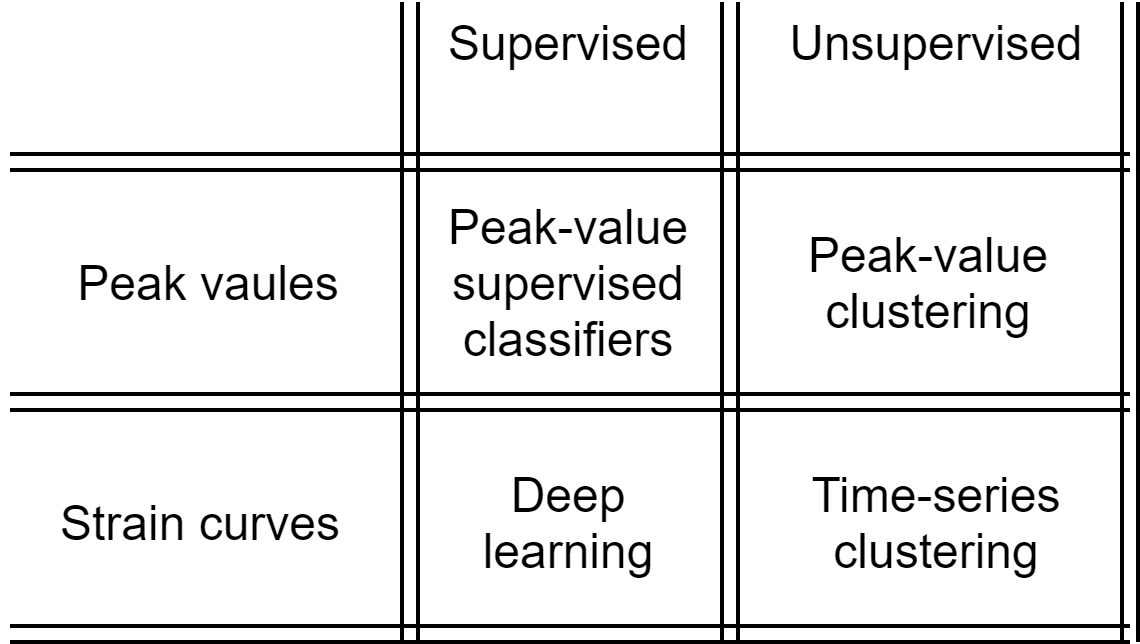
\includegraphics[width=0.5\textwidth]{intro/objectives_diagram.png}
    \caption{This is an illustration of the combinations of strain datasets and machine learning algorithms which will be tested in this work.}
    \label{fig:objectives_diagram}
\end{figure}

The objectives of this work can be summarized in the form of three questions:

\begin{tcolorbox}
    \textbf{Objectives}

    \begin{enumerate}
        \item Can a machine learning model be used to predict one of the three target variables assessed in this work using peak strain values or longitudinal strain curves?
        \item Which type of machine learning is best suited for predicting the aforementioned target variables, supervised or unsupervised learning models?
        \item Which type of input data works best for a machine learning model to predict the target variables, a dataset consisting of longitudinal strain curves or a dataset that consists of peak strain values in combination with \acrshort{ef}?
    \end{enumerate}
\end{tcolorbox}

\section{Structure}

The structure of this work is as follows: Chapter \ref{chap:strain} will explain the theory behind echocardiography, the technology used in ultrasound imaging, and outline the different heart diseases presented. Chapter \ref{chap:ml} describes the theory behind the machine learning models used. Chapter \ref{chap:lit} reviews the most recent work done on the topic. Chapter \ref{chap:data} explores the dataset. Chapter \ref{chap:method} details how every model in this work is configured, trained and evaluated. Chapter \ref{chap:results} presents the results of the individual models tested. A discussion of the results will be made in chapter \ref{chap:discussion} and a conclusion is given in chapter \ref{chap:conclusion}.
\chapter{Myocardial Imaging and Echocardiography} \label{chap:strain}

This chapter will describe the basic structure of the heart muscle, give an introduction to ultrasound imaging and echocardiography, explain how longitudinal strain curves and \acrfull{ef} are estimated, and give the definition of the different types of heart failure and myocardial infarction encountered in this work. The theory in this chapter on ultrasound imaging and echocardiography is mostly based on the work of Asbjørn Støylen, provided in his website ''Strain rate imaging''\footnote{http://folk.ntnu.no/stoylen/strainrate/} which is a collection of online articles on the physics and technology behind ultrasound imaging as used in echocardiography. The different online articles are referred to individually as separate works, to make it easier to find the exact source of the citation.

\section{Basic Cardiology}

The heart is an autonomous muscle that is responsible for pumping oxygenated blood from the lungs into the rest of the body and pumping unoxygenated blood from the rest of the body into the lungs. The heart can be divided into four separate chambers: The right atrium, the left atrium, the right ventricle, and the left ventricle. The right chambers are responsible for pumping unoxygenated blood from the body into the lungs, while the left chambers are responsible for pumping oxygenated blood from the lungs into the rest of the body. In both the right and left chambers, the blood flows first through the atria, and then through the ventricles before exiting the heart. One heart cycle is the period it takes the heart muscles to make a full contraction and relaxation. The period of the heart cycle where the heart relaxes and fills with blood is called the \textit{diastole}, and the period of the heart cycle when the heart contracts and pumps blood throughout the body is called the \textit{systole}. Cardiology is the branch of medicine that deals with the heart, and parts of the vascular system \cite{cardiology_wikipedia}. Cardiologists are doctors that specialize in the field of cardiology. Echocardiography is a diagnostic tool used in cardiology to make images of muscle tissue in the heart called myocard, using ultrasound technology. 

\section{Introduction to Ultrasound Imaging and Echocardiography}

Ultrasound imaging is a diagnostic tool that is popular because it can give videos in real-time, it is relatively inexpensive and has a lower associated health-risk compared to imaging alternatives \cite{medical_ultrasound_wikipedia}. In this section \textit{two dimensional B-mode ultrasound imaging} will be detailed, where the \textit{B} stands for \textit{brightness}. The frequency of the sound waves used in ultrasound imaging are in the range of 1 - 12 MHz, and the frequency chosen for wave pulses will decide the size of the objects that the method can resolve \cite{basic_ultrasound}. Ultrasound imaging works by emitting pulses of ultrasound waves at myocardial tissue, the pulses are partially reflected by the different tissue structures, and are then sampled by a receiver upon return at the source that transmitted them, as illustrated in figure \ref{fig:us_reflect}.

\begin{figure}[H]
    \centering
    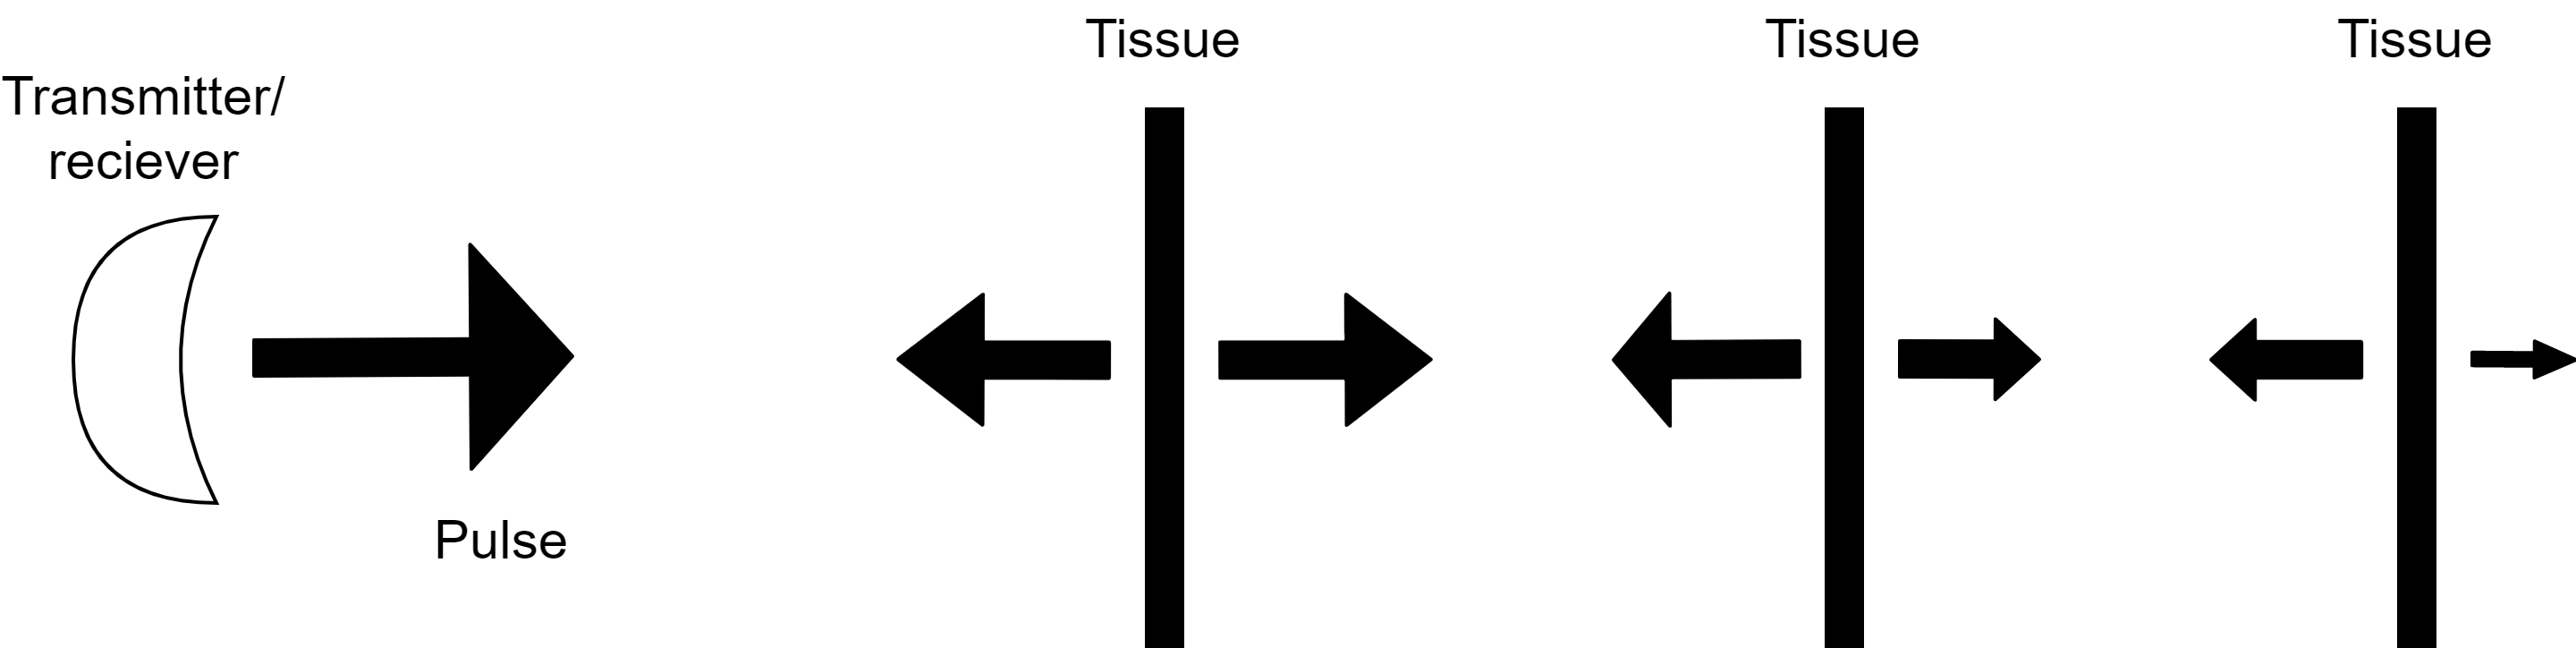
\includegraphics[width=0.99\textwidth]{echocardiography/US_reflection.png}
    \caption{An illustration of how ultrasound pulses are partially reflected by many barriers of tissue. The horisontal arrows represent the pulses, where the relative sizes represent the amplitude of the pulse, and the vertical lines represent different structures of tissue. The figure is inspired by figure 2 in \cite{basic_ultrasound}.}
    \label{fig:us_reflect}
\end{figure}

Sound waves will have different velocities depending on what medium it is traveling in. This ratio of velocities in the different mediums is what decides what amount of an incident wave is reflected when it hits a transition between two mediums. Since the velocities of the ultrasound waves in different mediums are known, and the time it takes for a transmitted pulse to return can be measured, one can calculate the distance to the tissue structure that reflected the transmitted pulse using equation \eqref{eq:dist}. 

\begin{equation}
    \mathrm{distance} = \frac{\mathrm{time}}{2 \times \mathrm{velocity}}
    \label{eq:dist}
\end{equation}

By plotting the intensity of the reflected pulses as a function of the distance to the point from which they are reflected, one gets what is called a \textit{B-mode line}. Images created by two-dimensional ultrasound imaging are polar plots of several B-mode lines that together make up a two-dimensional intersectional image of a tissue structure. The procedure consists of emitting a pulse, creating a B-mode line by the sampled reflections, rotating the transmitter, and repeating. This procedure is illustrated in figure \ref{fig:b_mode_search}.

\begin{figure}[H]
    \centering
    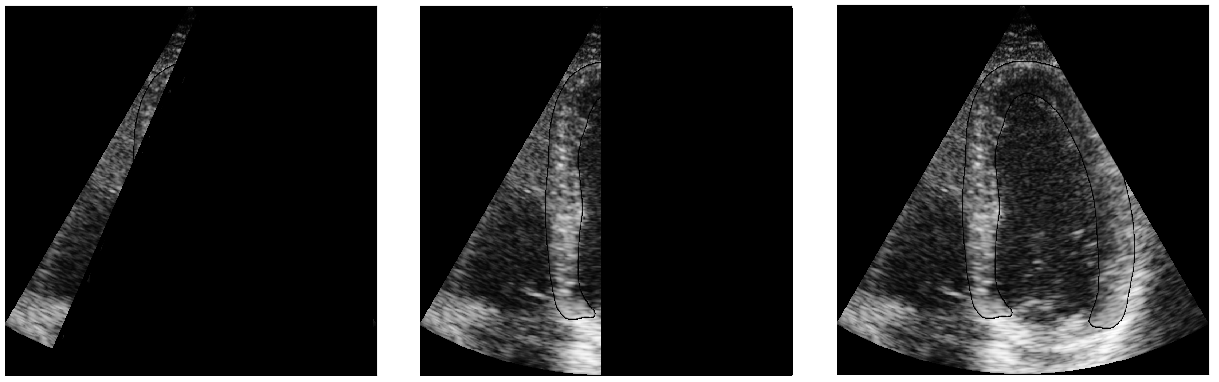
\includegraphics[width=0.99\textwidth]{echocardiography/b_mode_search.png}
    \caption{Illustration of how a two dimensional ultrasound image is put together by several individual B-mode lines. This figure is inspired by the graphical illustrations in figure 7 in \cite{basic_ultrasound}.}
    \label{fig:b_mode_search}
\end{figure}

The specific method of echocardiography used to collect the data used in this thesis is called transthoracic echocardiography. In this method, ultrasound images are produced by sending ultrasound waves through the ribs of a patient, from outside the body by locating the transmitter-receiver on the chest of the patient. The transthoracic echocardiography method is constricted by the ribs such that there are only three intersectional images that can be extracted from the heart. These three intersections are referred to as \textit{views}, and the corresponding terms are the \acrfull{4ch} view, \acrfull{2ch} view and the \acrfull{aplax} view, and examples of ultrasound images in all three views are given in figure \ref{fig:us_view_examples}.

\begin{figure}[H]
    \centering
    \begin{subfigure}[b]{0.3\textwidth} 
        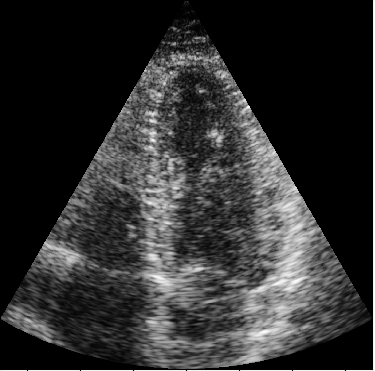
\includegraphics[width=0.99\textwidth]{echocardiography/4ch_frame.png}
        \caption{\acrshort{4ch}}
        \label{fig:us_view_examples_4ch}
    \end{subfigure}
    \begin{subfigure}[b]{0.3\textwidth}
        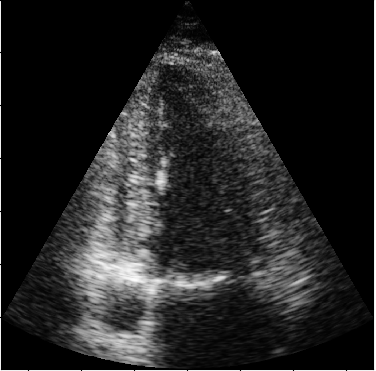
\includegraphics[width=0.99\textwidth]{echocardiography/2ch_frame.png}
        \caption{\acrshort{2ch}}
        \label{fig:us_view_examples_2ch}
    \end{subfigure}
    \begin{subfigure}[b]{0.3\textwidth}
        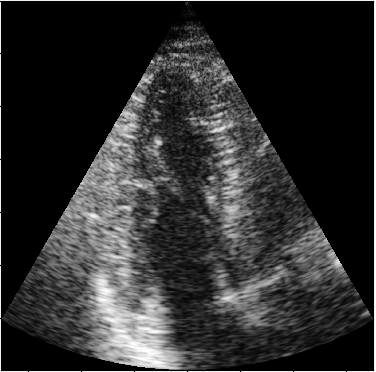
\includegraphics[width=0.99\textwidth]{echocardiography/aplax_frame.png}
        \caption{\acrshort{aplax}}
        \label{fig:us_view_examples_aplax}
    \end{subfigure}
    \caption{Examples of ultrasound images taken from the three views: (a) \acrfull{4ch}, (b) \acrfull{2ch} and (c) \acrfull{aplax}. Note that these images are flipped vertically because the ultrasound images are taken from below the heart.}
    \label{fig:us_view_examples}
\end{figure}

It is commonplace among clinicians to focus on the state of health of the left ventricle of the heart. In clinical procedure, the left ventricle is divided into 16, 17, or 18 segments. This work will follow the 18-segment model, as that is the model chosen by the clinician who has annotated the images. Figure \ref{fig:18_segment_model} illustrates the 18 different segments of the left ventricle, and how they can be seen in the different views. The names of the different segments are shown in table \ref{tab:segment_names}, where the segment numbers correspond to the numbers in figure \ref{fig:18_segment_model}. When referring to the entire intersection of the left ventricle that is visible from a particular view, it will be referred to as the \textit{global segment}.

\begin{table*}
    \centering
    \ra{1}
    \begin{tabular}{cc}
        \toprule
        Segment nr. & Segment name \\
        \midrule
        1           & Basal Septal  \\
        2           & Mid Septal  \\
        3           & Apical Septal  \\
        4           & Apical Lateral  \\
        5           & Mid Lateral  \\
        6           & Basal Lateral  \\
        7           & Basal Inferior  \\
        8           & Mid Inferior  \\
        9           & Apical Inferior  \\
        10          & Apical Anterior  \\
        11          & Mid Anterior  \\
        12          & Basal Anterior  \\
        13          & Basal Posterior  \\
        14          & Mid Posterior  \\
        15          & Apical Posterior  \\
        16          & Apical Anteroseptal  \\
        17          & Mid Anteroseptal  \\
        18          & Basal Anteroseptal  \\
        \bottomrule
    \end{tabular}
    \caption{A table matching the segment numbers shown in figure \ref{fig:18_segment_model}, with the segment name.}
    \label{tab:segment_names}
\end{table*}

\begin{figure}[H]
    \centering
    \begin{subfigure}[b]{0.3\textwidth} 
        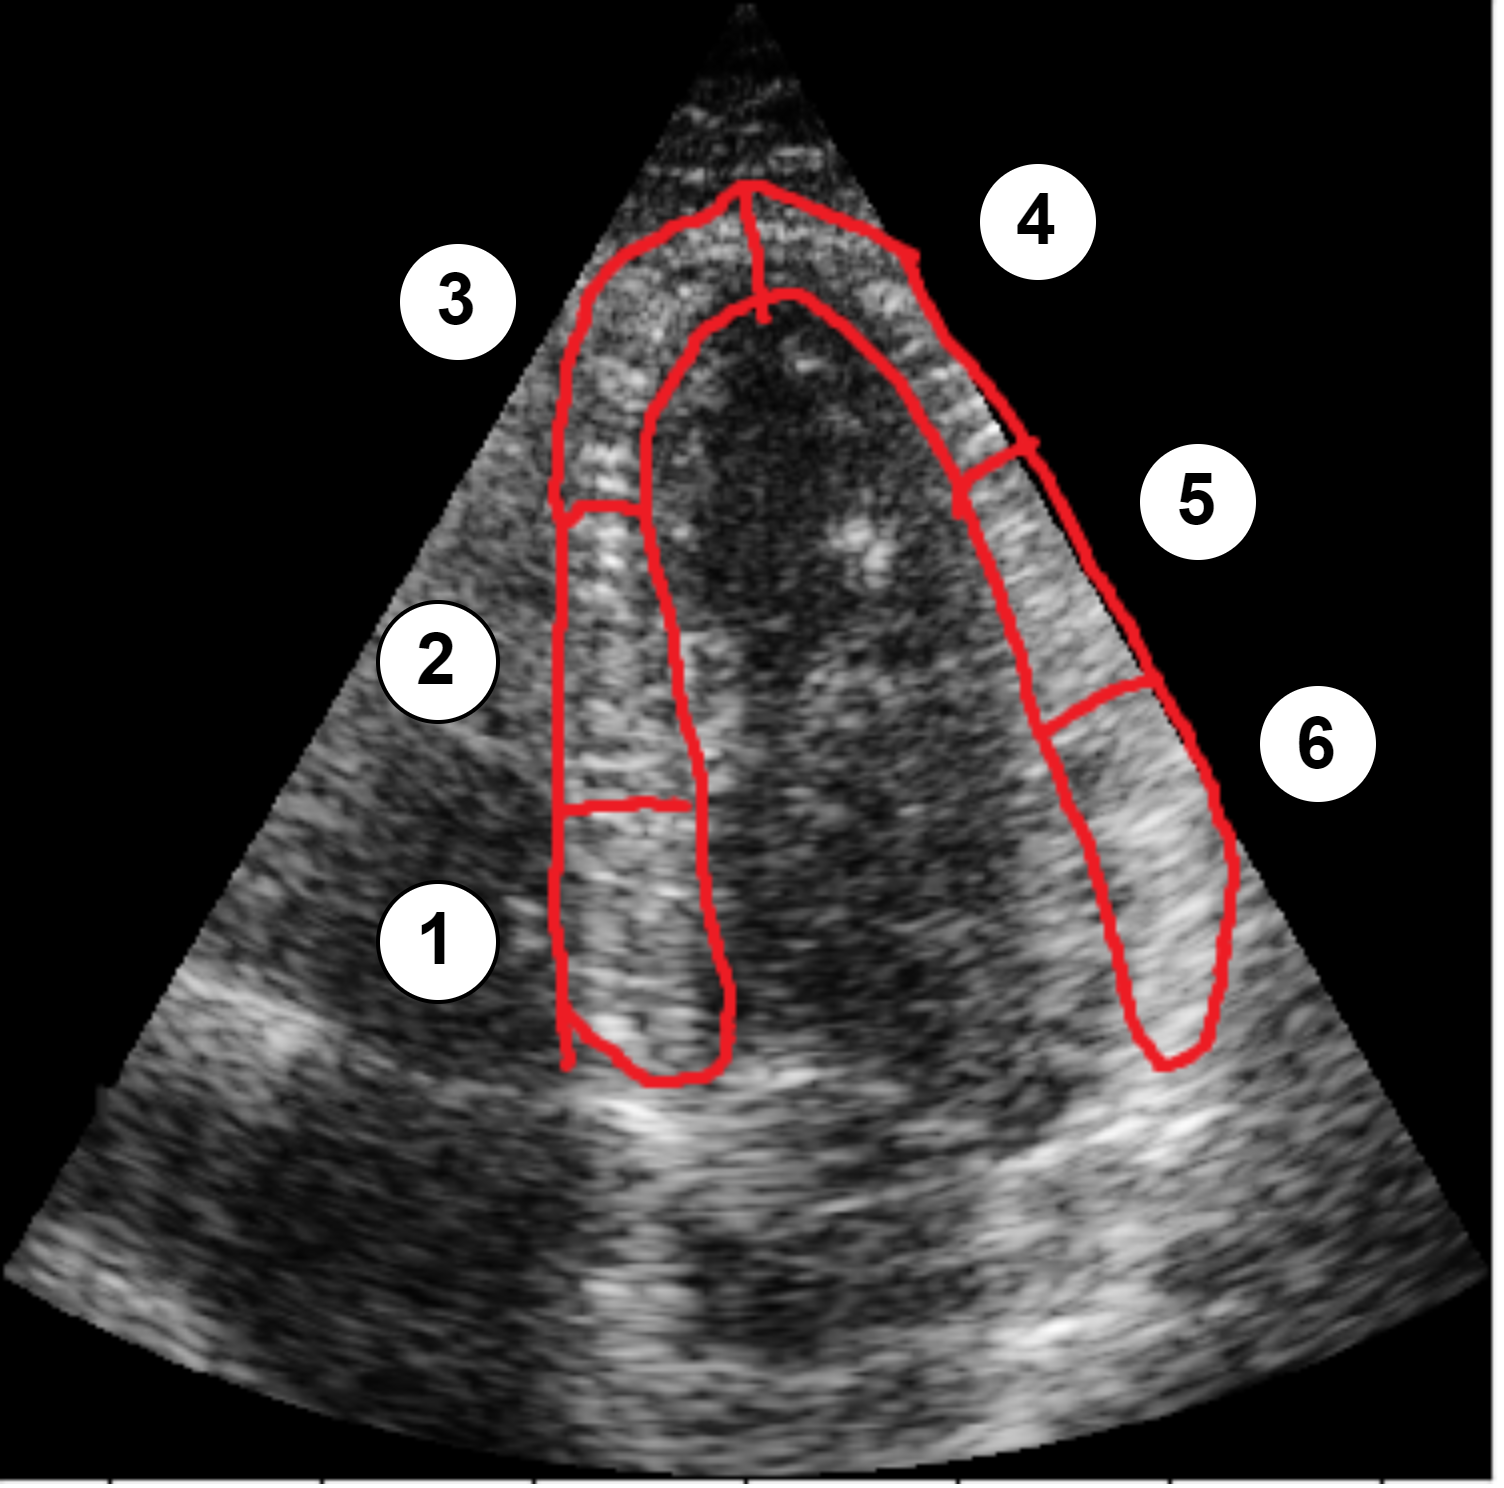
\includegraphics[width=0.99\textwidth]{echocardiography/4ch_frame_segmented.png}
        \caption{\acrshort{4ch}}
        \label{fig:18_segment_model_4ch}
    \end{subfigure}
    \begin{subfigure}[b]{0.3\textwidth}
        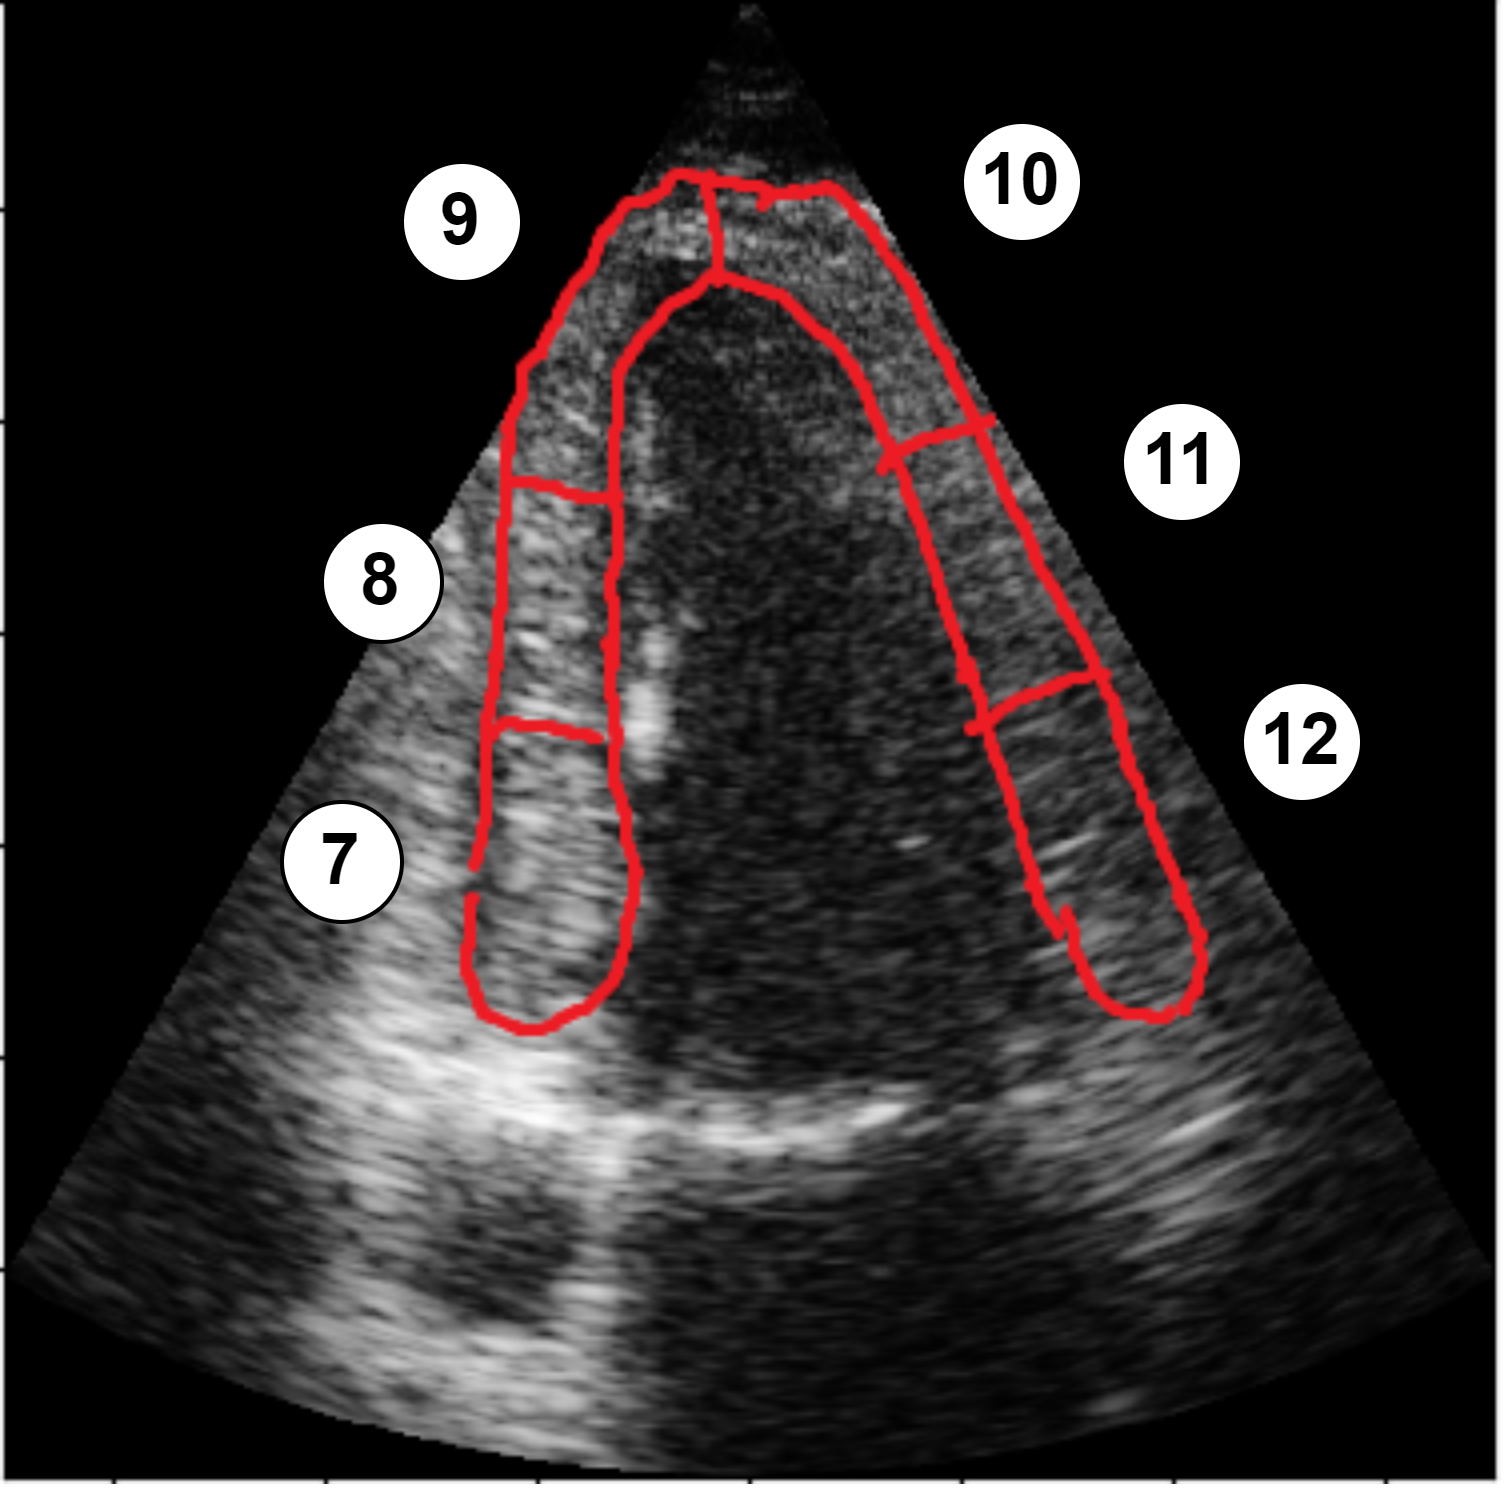
\includegraphics[width=0.99\textwidth]{echocardiography/2ch_frame_segmented.png}
        \caption{\acrshort{2ch}}
        \label{fig:18_segment_model_2ch}
    \end{subfigure}
    \begin{subfigure}[b]{0.3\textwidth}
        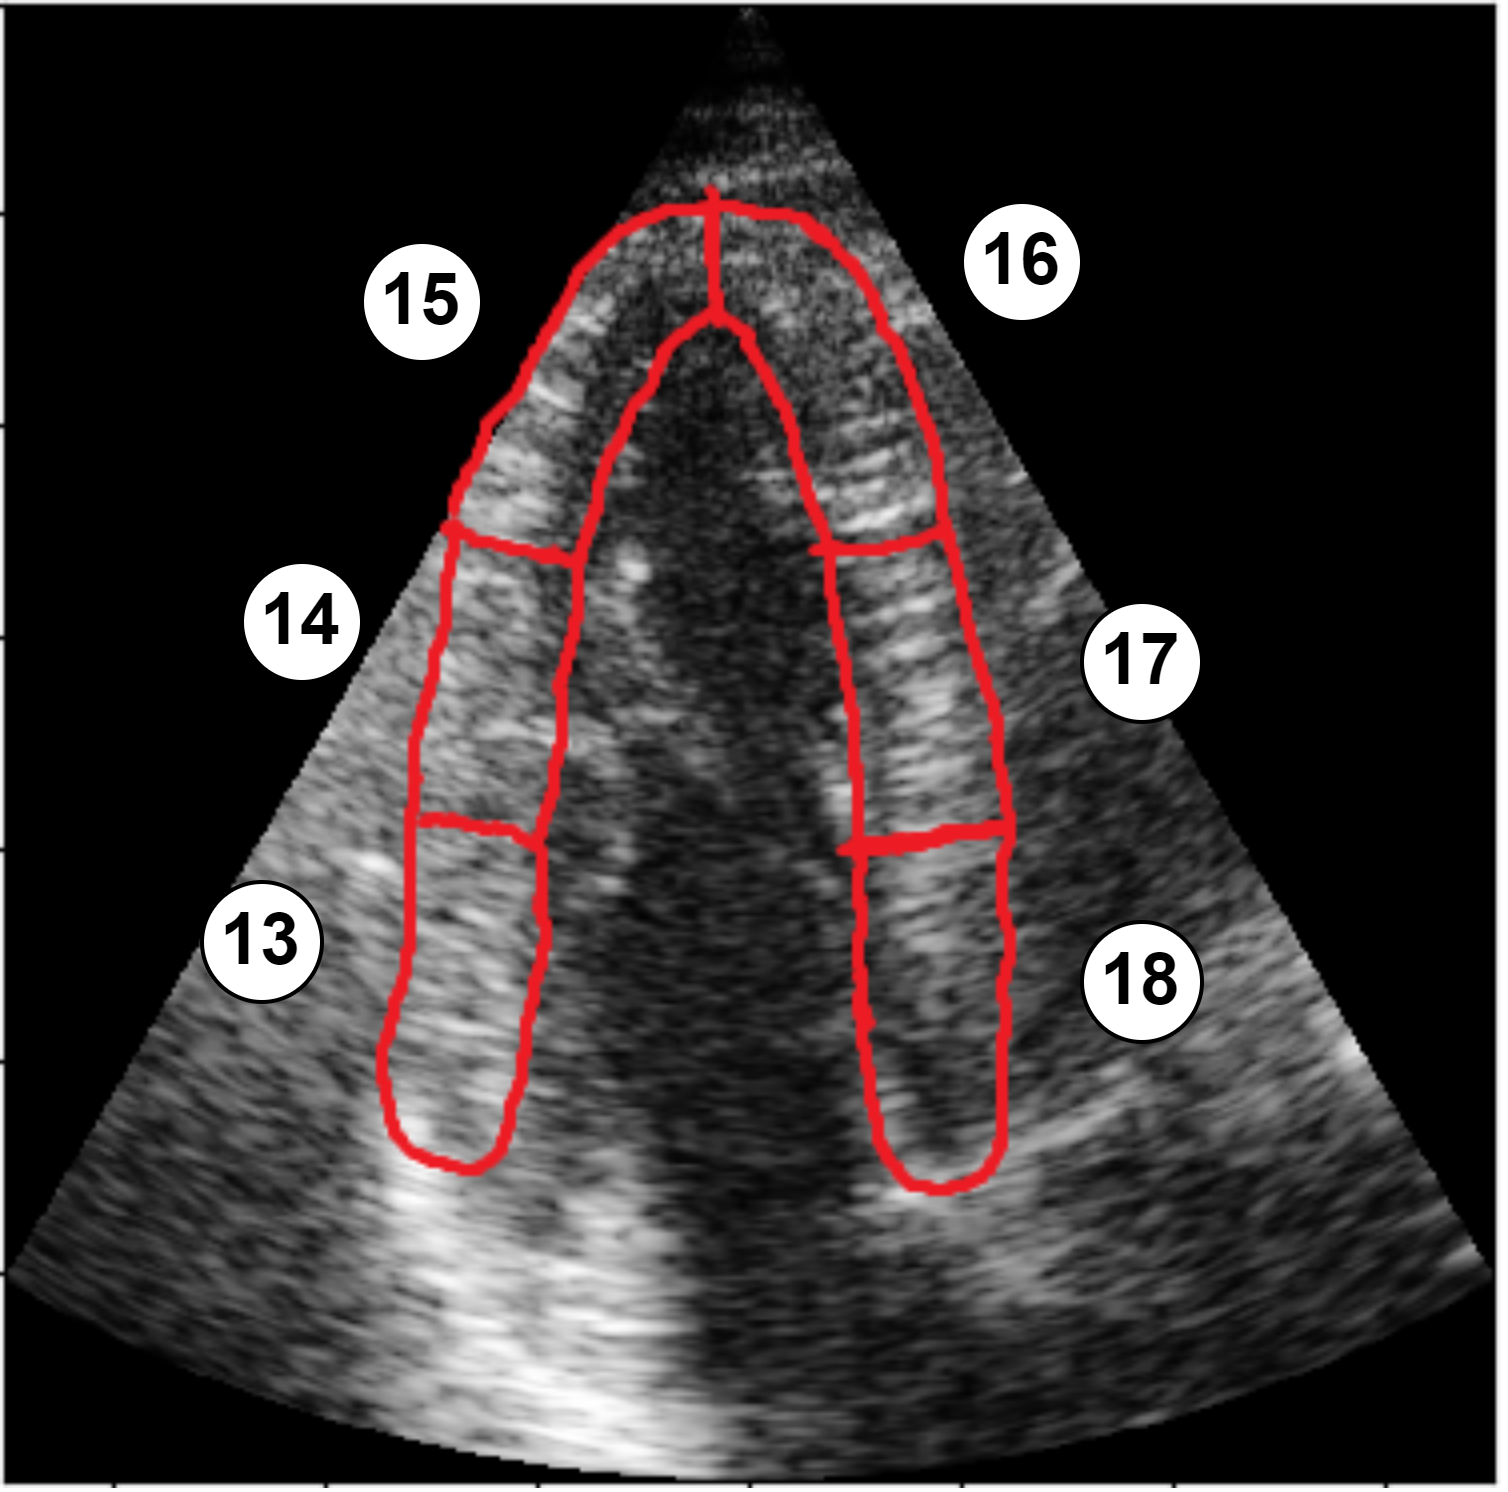
\includegraphics[width=0.99\textwidth]{echocardiography/aplax_frame_segmented.png}
        \caption{\acrshort{aplax}}
        \label{fig:18_segment_model_aplax}
    \end{subfigure}
    \caption{An illustration of the 18-segment model of the heart. It shows which segment can be seen in which view. Like in figure \ref{fig:us_view_examples} the images are flipped vertically. Note that the boundaries drawn on the figure are only meant to be illustrative, and are not the actual boundaries of the regional segments.}
    \label{fig:18_segment_model}
\end{figure}

\section{Myocardial Strain Estimation and Ejection Fraction} \label{sec:strain_est}

Strain is a relative measure of deformation, of physical objects. Since strain is relative, it has no unit and is measured in percentages in this work. The concept of strain is complex and is well established in other scientific fields such as structural engineering. When estimating strain of linear segments, one can use the Lagrangian formula defined in \eqref{eq:linear_strain} \cite{basic_concepts}. Let $L_r$ be the length of the segment at the reference time, let $t$ be the time one wishes to measure the strain at, let the length of the segment at $t$ be denoted $L_t$ and $\epsilon(t)$ be the strain. 

\begin{equation}
    \epsilon(t) = \frac{L_t - L_r}{L_r}
    \label{eq:linear_strain}
\end{equation}

This work will primarily be concerned with the longitudinal strain of segments in the left ventricle. The longitudinal strain occurs due to changes in the length of a myocardial segment. The two other types of strain that can be calculated with two-dimensional echocardiography are transmural strain, which is due to changes in the thickness of the myocard and circumferential strain, which are due to changes in the circumference of the entire structure \cite{basic_concepts}. To estimate the strain of a particular segment, one must first define the boundaries of all the segments. There are many ways of doing this, but the most accurate method is for a clinician to draw the segment borders by hand. The clinician that annotated the dataset used in this work segmented the images using the commercial tool ECHOPAC which is developed by GE HealthCare\footnote{https://www.gehealthcare.com/products/ultrasound/vivid/echopac}. The longitudinal strain of a segment is then the relative difference in length of a segment in image frame $t$ compared to a reference image. The length of a segment is illustrated with the centerline of the vertical segment borders in figure \ref{fig:strain_estimation}. The centerline is highlighted in red in figure \ref{fig:gls_estimation}, and blue in \ref{fig:rls_estimation}. As strain is a relative measure, one needs to define a reference length from which the other strain values are calculated with regard to. This could be the length of the segment during the first frame, the length of the segment when it is at its longest, the length of the segment when it is at its shortest, or the length of the segment in any other ultrasound image. The strain of a segment in the reference image will then be $0\%$, and the strain of the segment in the other images will be a percentage relative to the reference image. 

\begin{figure}[H]
    \centering
    \begin{subfigure}[b]{0.49\textwidth} 
        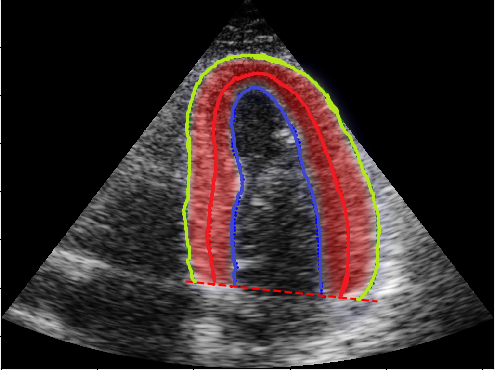
\includegraphics[width=0.99\textwidth, height=0.9\textwidth]{echocardiography/gls_estimation.png}
        \caption{\acrshort{gls} estimation}
        \label{fig:gls_estimation}
    \end{subfigure}
    \begin{subfigure}[b]{0.49\textwidth}
        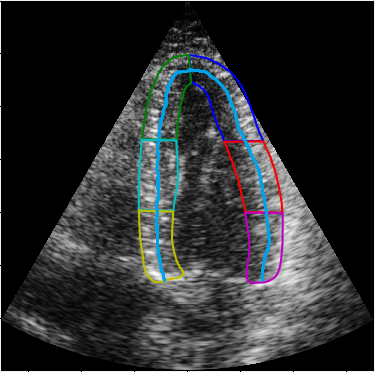
\includegraphics[width=0.99\textwidth, height=0.9\textwidth]{echocardiography/rls_estimation.png}
        \caption{\acrshort{rls} estimation}
        \label{fig:rls_estimation}
    \end{subfigure}
    \caption{Illustration meant to assist in the understanding of what longitudinal strain is. Note that the segment borders drawn on these images are only illustrative, and are not the actual segment borders used to estimate the strain. (a) shows the strain estimation of the global segment, and (b) shows the strain estimation of the regional segments.}
    \label{fig:strain_estimation}
\end{figure}

The IMPROVE dataset included computed strain curves, but it remains unclear exactly how they were computed. There are multiple ways of computing the strain of a segment, for example, the tissue Doppler and speckle tracking methods. As the name implies, the tissue Doppler method utilizes the Doppler effect. The Doppler effect can be concisely summarized by stating that when a wave is reflected by an object that has a velocity component that is radial with regard to the direction of the wave propagation, the frequency of the reflected wave will be changed with regard to the incident wave. The frequency will increase if the direction of the radial velocity component is opposite from the wave propagation direction, and it will decrease if the radial velocity component is in the same direction as the wave propagation. The magnitude of the frequency change can then be used to estimate the velocity of the moving object. Tissue Doppler then estimates the radial velocities of partitions of tissue to create a vector field of velocities \cite{strain_rate_imaging}. There are different ways of calculating strain from the velocity field, one option is to integrate the velocity field to track the displacement of the tissue partitions, but a method that requires less computation is to estimate the strain rate using equation \eqref{eq:strain_rate} \cite{myocardial_imaging}. Here $v_1$ and $v_2$ are the instantaneous velocities of the tissue partitions, and $\Delta x$ is a constant length. The strain is then estimated by integrating the strain rate over the total duration of the deformation. 

\begin{equation}
    \frac{\partial \epsilon}{\partial t} = \frac{v_2 - v_1}{\Delta x}
    \label{eq:strain_rate}
\end{equation}

The speckle tracking method is based on the fact that the spatial distribution of grey spots in an ultrasound image is inherently random. Specific regions of grey spots are referred to as speckle patterns, and each speckle pattern is unique. Since the speckle patterns are unique, their displacement can be tracked from one frame of the ultrasound video to another \cite{myocardial_imaging}. By then using the recorded longitudinal displacements of speckle patterns within a segment and equation \eqref{eq:linear_strain}, one can estimate the longitudinal strain of a segment.

By collecting all the strain values of a segment from the different ultrasound images into a time series, one gets a \textit{strain curve}. If the strain curve consists of strain values estimated from a global segment as depicted in figure \ref{fig:gls_estimation}, the curve is called a \acrfull{gls} curve. If the strain values are estimated from one of the six regional segments, as depicted in figure \ref{fig:rls_estimation}, the curves are called \acrfull{rls} curves. In diagnostic procedure, it is common to extract specific values from the longitudinal strain curves. Typical strain values extracted are the peak value during the systole, the peak value during the diastole, trough values during the systole, and trough values during the diastole. Figure \ref{fig:pss_illustration} shows what a typical longitudinal strain curve looks like. Blue dots on the strain curve illustrate the peak and trough strain values during systole. Red dots on the strain curve illustrate the peak and trough strain values during diastole. The color shading under the curves illustrates whether the heart cycle is in systole (blue), or diastole (red). In this work, one specific strain value will be tested as input data for classification models; the value that is extracted is the trough of the strain curve during the systole. This extracted strain value will be referred to as \textit{peak systolic strain}.

\begin{figure}[H]
    \centering
    %% Creator: Matplotlib, PGF backend
%%
%% To include the figure in your LaTeX document, write
%%   \input{<filename>.pgf}
%%
%% Make sure the required packages are loaded in your preamble
%%   \usepackage{pgf}
%%
%% Figures using additional raster images can only be included by \input if
%% they are in the same directory as the main LaTeX file. For loading figures
%% from other directories you can use the `import` package
%%   \usepackage{import}
%% and then include the figures with
%%   \import{<path to file>}{<filename>.pgf}
%%
%% Matplotlib used the following preamble
%%
\begingroup%
\makeatletter%
\begin{pgfpicture}%
\pgfpathrectangle{\pgfpointorigin}{\pgfqpoint{6.340000in}{2.540000in}}%
\pgfusepath{use as bounding box, clip}%
\begin{pgfscope}%
\pgfsetbuttcap%
\pgfsetmiterjoin%
\definecolor{currentfill}{rgb}{1.000000,1.000000,1.000000}%
\pgfsetfillcolor{currentfill}%
\pgfsetlinewidth{0.000000pt}%
\definecolor{currentstroke}{rgb}{1.000000,1.000000,1.000000}%
\pgfsetstrokecolor{currentstroke}%
\pgfsetdash{}{0pt}%
\pgfpathmoveto{\pgfqpoint{0.000000in}{0.000000in}}%
\pgfpathlineto{\pgfqpoint{6.340000in}{0.000000in}}%
\pgfpathlineto{\pgfqpoint{6.340000in}{2.540000in}}%
\pgfpathlineto{\pgfqpoint{0.000000in}{2.540000in}}%
\pgfpathclose%
\pgfusepath{fill}%
\end{pgfscope}%
\begin{pgfscope}%
\pgfsetbuttcap%
\pgfsetmiterjoin%
\definecolor{currentfill}{rgb}{0.917647,0.917647,0.949020}%
\pgfsetfillcolor{currentfill}%
\pgfsetlinewidth{0.000000pt}%
\definecolor{currentstroke}{rgb}{0.000000,0.000000,0.000000}%
\pgfsetstrokecolor{currentstroke}%
\pgfsetstrokeopacity{0.000000}%
\pgfsetdash{}{0pt}%
\pgfpathmoveto{\pgfqpoint{0.728470in}{0.602314in}}%
\pgfpathlineto{\pgfqpoint{6.240000in}{0.602314in}}%
\pgfpathlineto{\pgfqpoint{6.240000in}{2.440000in}}%
\pgfpathlineto{\pgfqpoint{0.728470in}{2.440000in}}%
\pgfpathclose%
\pgfusepath{fill}%
\end{pgfscope}%
\begin{pgfscope}%
\pgfpathrectangle{\pgfqpoint{0.728470in}{0.602314in}}{\pgfqpoint{5.511530in}{1.837686in}}%
\pgfusepath{clip}%
\pgfsetroundcap%
\pgfsetroundjoin%
\pgfsetlinewidth{1.003750pt}%
\definecolor{currentstroke}{rgb}{1.000000,1.000000,1.000000}%
\pgfsetstrokecolor{currentstroke}%
\pgfsetdash{}{0pt}%
\pgfpathmoveto{\pgfqpoint{0.978994in}{0.602314in}}%
\pgfpathlineto{\pgfqpoint{0.978994in}{2.440000in}}%
\pgfusepath{stroke}%
\end{pgfscope}%
\begin{pgfscope}%
\definecolor{textcolor}{rgb}{0.150000,0.150000,0.150000}%
\pgfsetstrokecolor{textcolor}%
\pgfsetfillcolor{textcolor}%
\pgftext[x=0.978994in,y=0.470370in,,top]{\color{textcolor}\sffamily\fontsize{12.000000}{14.400000}\selectfont \(\displaystyle 0.0\)}%
\end{pgfscope}%
\begin{pgfscope}%
\pgfpathrectangle{\pgfqpoint{0.728470in}{0.602314in}}{\pgfqpoint{5.511530in}{1.837686in}}%
\pgfusepath{clip}%
\pgfsetroundcap%
\pgfsetroundjoin%
\pgfsetlinewidth{1.003750pt}%
\definecolor{currentstroke}{rgb}{1.000000,1.000000,1.000000}%
\pgfsetstrokecolor{currentstroke}%
\pgfsetdash{}{0pt}%
\pgfpathmoveto{\pgfqpoint{1.620336in}{0.602314in}}%
\pgfpathlineto{\pgfqpoint{1.620336in}{2.440000in}}%
\pgfusepath{stroke}%
\end{pgfscope}%
\begin{pgfscope}%
\definecolor{textcolor}{rgb}{0.150000,0.150000,0.150000}%
\pgfsetstrokecolor{textcolor}%
\pgfsetfillcolor{textcolor}%
\pgftext[x=1.620336in,y=0.470370in,,top]{\color{textcolor}\sffamily\fontsize{12.000000}{14.400000}\selectfont \(\displaystyle 0.2\)}%
\end{pgfscope}%
\begin{pgfscope}%
\pgfpathrectangle{\pgfqpoint{0.728470in}{0.602314in}}{\pgfqpoint{5.511530in}{1.837686in}}%
\pgfusepath{clip}%
\pgfsetroundcap%
\pgfsetroundjoin%
\pgfsetlinewidth{1.003750pt}%
\definecolor{currentstroke}{rgb}{1.000000,1.000000,1.000000}%
\pgfsetstrokecolor{currentstroke}%
\pgfsetdash{}{0pt}%
\pgfpathmoveto{\pgfqpoint{2.261678in}{0.602314in}}%
\pgfpathlineto{\pgfqpoint{2.261678in}{2.440000in}}%
\pgfusepath{stroke}%
\end{pgfscope}%
\begin{pgfscope}%
\definecolor{textcolor}{rgb}{0.150000,0.150000,0.150000}%
\pgfsetstrokecolor{textcolor}%
\pgfsetfillcolor{textcolor}%
\pgftext[x=2.261678in,y=0.470370in,,top]{\color{textcolor}\sffamily\fontsize{12.000000}{14.400000}\selectfont \(\displaystyle 0.4\)}%
\end{pgfscope}%
\begin{pgfscope}%
\pgfpathrectangle{\pgfqpoint{0.728470in}{0.602314in}}{\pgfqpoint{5.511530in}{1.837686in}}%
\pgfusepath{clip}%
\pgfsetroundcap%
\pgfsetroundjoin%
\pgfsetlinewidth{1.003750pt}%
\definecolor{currentstroke}{rgb}{1.000000,1.000000,1.000000}%
\pgfsetstrokecolor{currentstroke}%
\pgfsetdash{}{0pt}%
\pgfpathmoveto{\pgfqpoint{2.903019in}{0.602314in}}%
\pgfpathlineto{\pgfqpoint{2.903019in}{2.440000in}}%
\pgfusepath{stroke}%
\end{pgfscope}%
\begin{pgfscope}%
\definecolor{textcolor}{rgb}{0.150000,0.150000,0.150000}%
\pgfsetstrokecolor{textcolor}%
\pgfsetfillcolor{textcolor}%
\pgftext[x=2.903019in,y=0.470370in,,top]{\color{textcolor}\sffamily\fontsize{12.000000}{14.400000}\selectfont \(\displaystyle 0.6\)}%
\end{pgfscope}%
\begin{pgfscope}%
\pgfpathrectangle{\pgfqpoint{0.728470in}{0.602314in}}{\pgfqpoint{5.511530in}{1.837686in}}%
\pgfusepath{clip}%
\pgfsetroundcap%
\pgfsetroundjoin%
\pgfsetlinewidth{1.003750pt}%
\definecolor{currentstroke}{rgb}{1.000000,1.000000,1.000000}%
\pgfsetstrokecolor{currentstroke}%
\pgfsetdash{}{0pt}%
\pgfpathmoveto{\pgfqpoint{3.544361in}{0.602314in}}%
\pgfpathlineto{\pgfqpoint{3.544361in}{2.440000in}}%
\pgfusepath{stroke}%
\end{pgfscope}%
\begin{pgfscope}%
\definecolor{textcolor}{rgb}{0.150000,0.150000,0.150000}%
\pgfsetstrokecolor{textcolor}%
\pgfsetfillcolor{textcolor}%
\pgftext[x=3.544361in,y=0.470370in,,top]{\color{textcolor}\sffamily\fontsize{12.000000}{14.400000}\selectfont \(\displaystyle 0.8\)}%
\end{pgfscope}%
\begin{pgfscope}%
\pgfpathrectangle{\pgfqpoint{0.728470in}{0.602314in}}{\pgfqpoint{5.511530in}{1.837686in}}%
\pgfusepath{clip}%
\pgfsetroundcap%
\pgfsetroundjoin%
\pgfsetlinewidth{1.003750pt}%
\definecolor{currentstroke}{rgb}{1.000000,1.000000,1.000000}%
\pgfsetstrokecolor{currentstroke}%
\pgfsetdash{}{0pt}%
\pgfpathmoveto{\pgfqpoint{4.185703in}{0.602314in}}%
\pgfpathlineto{\pgfqpoint{4.185703in}{2.440000in}}%
\pgfusepath{stroke}%
\end{pgfscope}%
\begin{pgfscope}%
\definecolor{textcolor}{rgb}{0.150000,0.150000,0.150000}%
\pgfsetstrokecolor{textcolor}%
\pgfsetfillcolor{textcolor}%
\pgftext[x=4.185703in,y=0.470370in,,top]{\color{textcolor}\sffamily\fontsize{12.000000}{14.400000}\selectfont \(\displaystyle 1.0\)}%
\end{pgfscope}%
\begin{pgfscope}%
\pgfpathrectangle{\pgfqpoint{0.728470in}{0.602314in}}{\pgfqpoint{5.511530in}{1.837686in}}%
\pgfusepath{clip}%
\pgfsetroundcap%
\pgfsetroundjoin%
\pgfsetlinewidth{1.003750pt}%
\definecolor{currentstroke}{rgb}{1.000000,1.000000,1.000000}%
\pgfsetstrokecolor{currentstroke}%
\pgfsetdash{}{0pt}%
\pgfpathmoveto{\pgfqpoint{4.827044in}{0.602314in}}%
\pgfpathlineto{\pgfqpoint{4.827044in}{2.440000in}}%
\pgfusepath{stroke}%
\end{pgfscope}%
\begin{pgfscope}%
\definecolor{textcolor}{rgb}{0.150000,0.150000,0.150000}%
\pgfsetstrokecolor{textcolor}%
\pgfsetfillcolor{textcolor}%
\pgftext[x=4.827044in,y=0.470370in,,top]{\color{textcolor}\sffamily\fontsize{12.000000}{14.400000}\selectfont \(\displaystyle 1.2\)}%
\end{pgfscope}%
\begin{pgfscope}%
\pgfpathrectangle{\pgfqpoint{0.728470in}{0.602314in}}{\pgfqpoint{5.511530in}{1.837686in}}%
\pgfusepath{clip}%
\pgfsetroundcap%
\pgfsetroundjoin%
\pgfsetlinewidth{1.003750pt}%
\definecolor{currentstroke}{rgb}{1.000000,1.000000,1.000000}%
\pgfsetstrokecolor{currentstroke}%
\pgfsetdash{}{0pt}%
\pgfpathmoveto{\pgfqpoint{5.468386in}{0.602314in}}%
\pgfpathlineto{\pgfqpoint{5.468386in}{2.440000in}}%
\pgfusepath{stroke}%
\end{pgfscope}%
\begin{pgfscope}%
\definecolor{textcolor}{rgb}{0.150000,0.150000,0.150000}%
\pgfsetstrokecolor{textcolor}%
\pgfsetfillcolor{textcolor}%
\pgftext[x=5.468386in,y=0.470370in,,top]{\color{textcolor}\sffamily\fontsize{12.000000}{14.400000}\selectfont \(\displaystyle 1.4\)}%
\end{pgfscope}%
\begin{pgfscope}%
\pgfpathrectangle{\pgfqpoint{0.728470in}{0.602314in}}{\pgfqpoint{5.511530in}{1.837686in}}%
\pgfusepath{clip}%
\pgfsetroundcap%
\pgfsetroundjoin%
\pgfsetlinewidth{1.003750pt}%
\definecolor{currentstroke}{rgb}{1.000000,1.000000,1.000000}%
\pgfsetstrokecolor{currentstroke}%
\pgfsetdash{}{0pt}%
\pgfpathmoveto{\pgfqpoint{6.109727in}{0.602314in}}%
\pgfpathlineto{\pgfqpoint{6.109727in}{2.440000in}}%
\pgfusepath{stroke}%
\end{pgfscope}%
\begin{pgfscope}%
\definecolor{textcolor}{rgb}{0.150000,0.150000,0.150000}%
\pgfsetstrokecolor{textcolor}%
\pgfsetfillcolor{textcolor}%
\pgftext[x=6.109727in,y=0.470370in,,top]{\color{textcolor}\sffamily\fontsize{12.000000}{14.400000}\selectfont \(\displaystyle 1.6\)}%
\end{pgfscope}%
\begin{pgfscope}%
\definecolor{textcolor}{rgb}{0.150000,0.150000,0.150000}%
\pgfsetstrokecolor{textcolor}%
\pgfsetfillcolor{textcolor}%
\pgftext[x=3.484235in,y=0.266667in,,top]{\color{textcolor}\sffamily\fontsize{12.000000}{14.400000}\selectfont Time [s]}%
\end{pgfscope}%
\begin{pgfscope}%
\pgfpathrectangle{\pgfqpoint{0.728470in}{0.602314in}}{\pgfqpoint{5.511530in}{1.837686in}}%
\pgfusepath{clip}%
\pgfsetroundcap%
\pgfsetroundjoin%
\pgfsetlinewidth{1.003750pt}%
\definecolor{currentstroke}{rgb}{1.000000,1.000000,1.000000}%
\pgfsetstrokecolor{currentstroke}%
\pgfsetdash{}{0pt}%
\pgfpathmoveto{\pgfqpoint{0.728470in}{1.105106in}}%
\pgfpathlineto{\pgfqpoint{6.240000in}{1.105106in}}%
\pgfusepath{stroke}%
\end{pgfscope}%
\begin{pgfscope}%
\definecolor{textcolor}{rgb}{0.150000,0.150000,0.150000}%
\pgfsetstrokecolor{textcolor}%
\pgfsetfillcolor{textcolor}%
\pgftext[x=0.303703in,y=1.047235in,left,base]{\color{textcolor}\sffamily\fontsize{12.000000}{14.400000}\selectfont \(\displaystyle -10\)}%
\end{pgfscope}%
\begin{pgfscope}%
\pgfpathrectangle{\pgfqpoint{0.728470in}{0.602314in}}{\pgfqpoint{5.511530in}{1.837686in}}%
\pgfusepath{clip}%
\pgfsetroundcap%
\pgfsetroundjoin%
\pgfsetlinewidth{1.003750pt}%
\definecolor{currentstroke}{rgb}{1.000000,1.000000,1.000000}%
\pgfsetstrokecolor{currentstroke}%
\pgfsetdash{}{0pt}%
\pgfpathmoveto{\pgfqpoint{0.728470in}{1.704049in}}%
\pgfpathlineto{\pgfqpoint{6.240000in}{1.704049in}}%
\pgfusepath{stroke}%
\end{pgfscope}%
\begin{pgfscope}%
\definecolor{textcolor}{rgb}{0.150000,0.150000,0.150000}%
\pgfsetstrokecolor{textcolor}%
\pgfsetfillcolor{textcolor}%
\pgftext[x=0.385299in,y=1.646179in,left,base]{\color{textcolor}\sffamily\fontsize{12.000000}{14.400000}\selectfont \(\displaystyle -5\)}%
\end{pgfscope}%
\begin{pgfscope}%
\pgfpathrectangle{\pgfqpoint{0.728470in}{0.602314in}}{\pgfqpoint{5.511530in}{1.837686in}}%
\pgfusepath{clip}%
\pgfsetroundcap%
\pgfsetroundjoin%
\pgfsetlinewidth{1.003750pt}%
\definecolor{currentstroke}{rgb}{1.000000,1.000000,1.000000}%
\pgfsetstrokecolor{currentstroke}%
\pgfsetdash{}{0pt}%
\pgfpathmoveto{\pgfqpoint{0.728470in}{2.302992in}}%
\pgfpathlineto{\pgfqpoint{6.240000in}{2.302992in}}%
\pgfusepath{stroke}%
\end{pgfscope}%
\begin{pgfscope}%
\definecolor{textcolor}{rgb}{0.150000,0.150000,0.150000}%
\pgfsetstrokecolor{textcolor}%
\pgfsetfillcolor{textcolor}%
\pgftext[x=0.514929in,y=2.245122in,left,base]{\color{textcolor}\sffamily\fontsize{12.000000}{14.400000}\selectfont \(\displaystyle 0\)}%
\end{pgfscope}%
\begin{pgfscope}%
\definecolor{textcolor}{rgb}{0.150000,0.150000,0.150000}%
\pgfsetstrokecolor{textcolor}%
\pgfsetfillcolor{textcolor}%
\pgftext[x=0.248148in,y=1.521157in,,bottom,rotate=90.000000]{\color{textcolor}\sffamily\fontsize{12.000000}{14.400000}\selectfont Strain}%
\end{pgfscope}%
\begin{pgfscope}%
\pgfpathrectangle{\pgfqpoint{0.728470in}{0.602314in}}{\pgfqpoint{5.511530in}{1.837686in}}%
\pgfusepath{clip}%
\pgfsetbuttcap%
\pgfsetroundjoin%
\definecolor{currentfill}{rgb}{0.298039,0.447059,0.690196}%
\pgfsetfillcolor{currentfill}%
\pgfsetfillopacity{0.300000}%
\pgfsetlinewidth{1.003750pt}%
\definecolor{currentstroke}{rgb}{0.298039,0.447059,0.690196}%
\pgfsetstrokecolor{currentstroke}%
\pgfsetstrokeopacity{0.300000}%
\pgfsetdash{}{0pt}%
\pgfpathmoveto{\pgfqpoint{0.978994in}{1.962271in}}%
\pgfpathlineto{\pgfqpoint{0.978994in}{0.685845in}}%
\pgfpathlineto{\pgfqpoint{1.029099in}{0.685845in}}%
\pgfpathlineto{\pgfqpoint{1.079204in}{0.685845in}}%
\pgfpathlineto{\pgfqpoint{1.129309in}{0.685845in}}%
\pgfpathlineto{\pgfqpoint{1.179414in}{0.685845in}}%
\pgfpathlineto{\pgfqpoint{1.229518in}{0.685845in}}%
\pgfpathlineto{\pgfqpoint{1.279623in}{0.685845in}}%
\pgfpathlineto{\pgfqpoint{1.329728in}{0.685845in}}%
\pgfpathlineto{\pgfqpoint{1.379833in}{0.685845in}}%
\pgfpathlineto{\pgfqpoint{1.429938in}{0.685845in}}%
\pgfpathlineto{\pgfqpoint{1.480043in}{0.685845in}}%
\pgfpathlineto{\pgfqpoint{1.530147in}{0.685845in}}%
\pgfpathlineto{\pgfqpoint{1.580252in}{0.685845in}}%
\pgfpathlineto{\pgfqpoint{1.630357in}{0.685845in}}%
\pgfpathlineto{\pgfqpoint{1.680462in}{0.685845in}}%
\pgfpathlineto{\pgfqpoint{1.730567in}{0.685845in}}%
\pgfpathlineto{\pgfqpoint{1.780671in}{0.685845in}}%
\pgfpathlineto{\pgfqpoint{1.830776in}{0.685845in}}%
\pgfpathlineto{\pgfqpoint{1.880881in}{0.685845in}}%
\pgfpathlineto{\pgfqpoint{1.930986in}{0.685845in}}%
\pgfpathlineto{\pgfqpoint{1.981091in}{0.685845in}}%
\pgfpathlineto{\pgfqpoint{2.031195in}{0.685845in}}%
\pgfpathlineto{\pgfqpoint{2.081300in}{0.685845in}}%
\pgfpathlineto{\pgfqpoint{2.131405in}{0.685845in}}%
\pgfpathlineto{\pgfqpoint{2.181510in}{0.685845in}}%
\pgfpathlineto{\pgfqpoint{2.231615in}{0.685845in}}%
\pgfpathlineto{\pgfqpoint{2.281720in}{0.685845in}}%
\pgfpathlineto{\pgfqpoint{2.331824in}{0.685845in}}%
\pgfpathlineto{\pgfqpoint{2.381929in}{0.685845in}}%
\pgfpathlineto{\pgfqpoint{2.432034in}{0.685845in}}%
\pgfpathlineto{\pgfqpoint{2.482139in}{0.685845in}}%
\pgfpathlineto{\pgfqpoint{2.532244in}{0.685845in}}%
\pgfpathlineto{\pgfqpoint{2.582348in}{0.685845in}}%
\pgfpathlineto{\pgfqpoint{2.632453in}{0.685845in}}%
\pgfpathlineto{\pgfqpoint{2.682558in}{0.685845in}}%
\pgfpathlineto{\pgfqpoint{2.732663in}{0.685845in}}%
\pgfpathlineto{\pgfqpoint{2.782768in}{0.685845in}}%
\pgfpathlineto{\pgfqpoint{2.832873in}{0.685845in}}%
\pgfpathlineto{\pgfqpoint{2.882977in}{0.685845in}}%
\pgfpathlineto{\pgfqpoint{2.933082in}{0.685845in}}%
\pgfpathlineto{\pgfqpoint{2.983187in}{0.685845in}}%
\pgfpathlineto{\pgfqpoint{3.033292in}{0.685845in}}%
\pgfpathlineto{\pgfqpoint{3.083397in}{0.685845in}}%
\pgfpathlineto{\pgfqpoint{3.133501in}{0.685845in}}%
\pgfpathlineto{\pgfqpoint{3.183606in}{0.685845in}}%
\pgfpathlineto{\pgfqpoint{3.183606in}{0.811826in}}%
\pgfpathlineto{\pgfqpoint{3.183606in}{0.811826in}}%
\pgfpathlineto{\pgfqpoint{3.133501in}{0.783501in}}%
\pgfpathlineto{\pgfqpoint{3.083397in}{0.774631in}}%
\pgfpathlineto{\pgfqpoint{3.033292in}{0.769909in}}%
\pgfpathlineto{\pgfqpoint{2.983187in}{0.763368in}}%
\pgfpathlineto{\pgfqpoint{2.933082in}{0.755592in}}%
\pgfpathlineto{\pgfqpoint{2.882977in}{0.748173in}}%
\pgfpathlineto{\pgfqpoint{2.832873in}{0.740620in}}%
\pgfpathlineto{\pgfqpoint{2.782768in}{0.731824in}}%
\pgfpathlineto{\pgfqpoint{2.732663in}{0.723730in}}%
\pgfpathlineto{\pgfqpoint{2.682558in}{0.722012in}}%
\pgfpathlineto{\pgfqpoint{2.632453in}{0.733274in}}%
\pgfpathlineto{\pgfqpoint{2.582348in}{0.761881in}}%
\pgfpathlineto{\pgfqpoint{2.532244in}{0.807844in}}%
\pgfpathlineto{\pgfqpoint{2.482139in}{0.866719in}}%
\pgfpathlineto{\pgfqpoint{2.432034in}{0.934317in}}%
\pgfpathlineto{\pgfqpoint{2.381929in}{1.010635in}}%
\pgfpathlineto{\pgfqpoint{2.331824in}{1.100265in}}%
\pgfpathlineto{\pgfqpoint{2.281720in}{1.208523in}}%
\pgfpathlineto{\pgfqpoint{2.231615in}{1.334555in}}%
\pgfpathlineto{\pgfqpoint{2.181510in}{1.469757in}}%
\pgfpathlineto{\pgfqpoint{2.131405in}{1.605028in}}%
\pgfpathlineto{\pgfqpoint{2.081300in}{1.736193in}}%
\pgfpathlineto{\pgfqpoint{2.031195in}{1.860088in}}%
\pgfpathlineto{\pgfqpoint{1.981091in}{1.971364in}}%
\pgfpathlineto{\pgfqpoint{1.930986in}{2.066555in}}%
\pgfpathlineto{\pgfqpoint{1.880881in}{2.145999in}}%
\pgfpathlineto{\pgfqpoint{1.830776in}{2.211525in}}%
\pgfpathlineto{\pgfqpoint{1.780671in}{2.260978in}}%
\pgfpathlineto{\pgfqpoint{1.730567in}{2.291380in}}%
\pgfpathlineto{\pgfqpoint{1.680462in}{2.302992in}}%
\pgfpathlineto{\pgfqpoint{1.630357in}{2.301584in}}%
\pgfpathlineto{\pgfqpoint{1.580252in}{2.292281in}}%
\pgfpathlineto{\pgfqpoint{1.530147in}{2.272969in}}%
\pgfpathlineto{\pgfqpoint{1.480043in}{2.235568in}}%
\pgfpathlineto{\pgfqpoint{1.429938in}{2.176100in}}%
\pgfpathlineto{\pgfqpoint{1.379833in}{2.103664in}}%
\pgfpathlineto{\pgfqpoint{1.329728in}{2.037376in}}%
\pgfpathlineto{\pgfqpoint{1.279623in}{1.991957in}}%
\pgfpathlineto{\pgfqpoint{1.229518in}{1.968768in}}%
\pgfpathlineto{\pgfqpoint{1.179414in}{1.960291in}}%
\pgfpathlineto{\pgfqpoint{1.129309in}{1.958907in}}%
\pgfpathlineto{\pgfqpoint{1.079204in}{1.959958in}}%
\pgfpathlineto{\pgfqpoint{1.029099in}{1.961253in}}%
\pgfpathlineto{\pgfqpoint{0.978994in}{1.962271in}}%
\pgfpathclose%
\pgfusepath{stroke,fill}%
\end{pgfscope}%
\begin{pgfscope}%
\pgfpathrectangle{\pgfqpoint{0.728470in}{0.602314in}}{\pgfqpoint{5.511530in}{1.837686in}}%
\pgfusepath{clip}%
\pgfsetbuttcap%
\pgfsetroundjoin%
\definecolor{currentfill}{rgb}{0.768627,0.305882,0.321569}%
\pgfsetfillcolor{currentfill}%
\pgfsetfillopacity{0.300000}%
\pgfsetlinewidth{1.003750pt}%
\definecolor{currentstroke}{rgb}{0.768627,0.305882,0.321569}%
\pgfsetstrokecolor{currentstroke}%
\pgfsetstrokeopacity{0.300000}%
\pgfsetdash{}{0pt}%
\pgfpathmoveto{\pgfqpoint{3.233711in}{0.878046in}}%
\pgfpathlineto{\pgfqpoint{3.233711in}{0.685845in}}%
\pgfpathlineto{\pgfqpoint{3.283816in}{0.685845in}}%
\pgfpathlineto{\pgfqpoint{3.333921in}{0.685845in}}%
\pgfpathlineto{\pgfqpoint{3.384026in}{0.685845in}}%
\pgfpathlineto{\pgfqpoint{3.434130in}{0.685845in}}%
\pgfpathlineto{\pgfqpoint{3.484235in}{0.685845in}}%
\pgfpathlineto{\pgfqpoint{3.534340in}{0.685845in}}%
\pgfpathlineto{\pgfqpoint{3.584445in}{0.685845in}}%
\pgfpathlineto{\pgfqpoint{3.634550in}{0.685845in}}%
\pgfpathlineto{\pgfqpoint{3.684654in}{0.685845in}}%
\pgfpathlineto{\pgfqpoint{3.734759in}{0.685845in}}%
\pgfpathlineto{\pgfqpoint{3.784864in}{0.685845in}}%
\pgfpathlineto{\pgfqpoint{3.834969in}{0.685845in}}%
\pgfpathlineto{\pgfqpoint{3.885074in}{0.685845in}}%
\pgfpathlineto{\pgfqpoint{3.935178in}{0.685845in}}%
\pgfpathlineto{\pgfqpoint{3.985283in}{0.685845in}}%
\pgfpathlineto{\pgfqpoint{4.035388in}{0.685845in}}%
\pgfpathlineto{\pgfqpoint{4.085493in}{0.685845in}}%
\pgfpathlineto{\pgfqpoint{4.135598in}{0.685845in}}%
\pgfpathlineto{\pgfqpoint{4.185703in}{0.685845in}}%
\pgfpathlineto{\pgfqpoint{4.235807in}{0.685845in}}%
\pgfpathlineto{\pgfqpoint{4.285912in}{0.685845in}}%
\pgfpathlineto{\pgfqpoint{4.336017in}{0.685845in}}%
\pgfpathlineto{\pgfqpoint{4.386122in}{0.685845in}}%
\pgfpathlineto{\pgfqpoint{4.436227in}{0.685845in}}%
\pgfpathlineto{\pgfqpoint{4.486331in}{0.685845in}}%
\pgfpathlineto{\pgfqpoint{4.536436in}{0.685845in}}%
\pgfpathlineto{\pgfqpoint{4.586541in}{0.685845in}}%
\pgfpathlineto{\pgfqpoint{4.636646in}{0.685845in}}%
\pgfpathlineto{\pgfqpoint{4.686751in}{0.685845in}}%
\pgfpathlineto{\pgfqpoint{4.736856in}{0.685845in}}%
\pgfpathlineto{\pgfqpoint{4.786960in}{0.685845in}}%
\pgfpathlineto{\pgfqpoint{4.837065in}{0.685845in}}%
\pgfpathlineto{\pgfqpoint{4.887170in}{0.685845in}}%
\pgfpathlineto{\pgfqpoint{4.937275in}{0.685845in}}%
\pgfpathlineto{\pgfqpoint{4.987380in}{0.685845in}}%
\pgfpathlineto{\pgfqpoint{5.037484in}{0.685845in}}%
\pgfpathlineto{\pgfqpoint{5.087589in}{0.685845in}}%
\pgfpathlineto{\pgfqpoint{5.137694in}{0.685845in}}%
\pgfpathlineto{\pgfqpoint{5.187799in}{0.685845in}}%
\pgfpathlineto{\pgfqpoint{5.237904in}{0.685845in}}%
\pgfpathlineto{\pgfqpoint{5.288009in}{0.685845in}}%
\pgfpathlineto{\pgfqpoint{5.338113in}{0.685845in}}%
\pgfpathlineto{\pgfqpoint{5.388218in}{0.685845in}}%
\pgfpathlineto{\pgfqpoint{5.438323in}{0.685845in}}%
\pgfpathlineto{\pgfqpoint{5.488428in}{0.685845in}}%
\pgfpathlineto{\pgfqpoint{5.538533in}{0.685845in}}%
\pgfpathlineto{\pgfqpoint{5.588637in}{0.685845in}}%
\pgfpathlineto{\pgfqpoint{5.638742in}{0.685845in}}%
\pgfpathlineto{\pgfqpoint{5.688847in}{0.685845in}}%
\pgfpathlineto{\pgfqpoint{5.738952in}{0.685845in}}%
\pgfpathlineto{\pgfqpoint{5.789057in}{0.685845in}}%
\pgfpathlineto{\pgfqpoint{5.839161in}{0.685845in}}%
\pgfpathlineto{\pgfqpoint{5.889266in}{0.685845in}}%
\pgfpathlineto{\pgfqpoint{5.939371in}{0.685845in}}%
\pgfpathlineto{\pgfqpoint{5.989476in}{0.685845in}}%
\pgfpathlineto{\pgfqpoint{5.989476in}{0.707198in}}%
\pgfpathlineto{\pgfqpoint{5.989476in}{0.707198in}}%
\pgfpathlineto{\pgfqpoint{5.939371in}{0.818465in}}%
\pgfpathlineto{\pgfqpoint{5.889266in}{0.943302in}}%
\pgfpathlineto{\pgfqpoint{5.839161in}{1.082254in}}%
\pgfpathlineto{\pgfqpoint{5.789057in}{1.226614in}}%
\pgfpathlineto{\pgfqpoint{5.738952in}{1.369412in}}%
\pgfpathlineto{\pgfqpoint{5.688847in}{1.508296in}}%
\pgfpathlineto{\pgfqpoint{5.638742in}{1.642391in}}%
\pgfpathlineto{\pgfqpoint{5.588637in}{1.771733in}}%
\pgfpathlineto{\pgfqpoint{5.538533in}{1.896957in}}%
\pgfpathlineto{\pgfqpoint{5.488428in}{2.016190in}}%
\pgfpathlineto{\pgfqpoint{5.438323in}{2.122016in}}%
\pgfpathlineto{\pgfqpoint{5.388218in}{2.206623in}}%
\pgfpathlineto{\pgfqpoint{5.338113in}{2.266566in}}%
\pgfpathlineto{\pgfqpoint{5.288009in}{2.302992in}}%
\pgfpathlineto{\pgfqpoint{5.237904in}{2.319213in}}%
\pgfpathlineto{\pgfqpoint{5.187799in}{2.319285in}}%
\pgfpathlineto{\pgfqpoint{5.137694in}{2.306209in}}%
\pgfpathlineto{\pgfqpoint{5.087589in}{2.281027in}}%
\pgfpathlineto{\pgfqpoint{5.037484in}{2.244337in}}%
\pgfpathlineto{\pgfqpoint{4.987380in}{2.199168in}}%
\pgfpathlineto{\pgfqpoint{4.937275in}{2.152361in}}%
\pgfpathlineto{\pgfqpoint{4.887170in}{2.111916in}}%
\pgfpathlineto{\pgfqpoint{4.837065in}{2.083609in}}%
\pgfpathlineto{\pgfqpoint{4.786960in}{2.067567in}}%
\pgfpathlineto{\pgfqpoint{4.736856in}{2.059242in}}%
\pgfpathlineto{\pgfqpoint{4.686751in}{2.053593in}}%
\pgfpathlineto{\pgfqpoint{4.636646in}{2.048548in}}%
\pgfpathlineto{\pgfqpoint{4.586541in}{2.045927in}}%
\pgfpathlineto{\pgfqpoint{4.536436in}{2.048988in}}%
\pgfpathlineto{\pgfqpoint{4.486331in}{2.058466in}}%
\pgfpathlineto{\pgfqpoint{4.436227in}{2.071259in}}%
\pgfpathlineto{\pgfqpoint{4.386122in}{2.084171in}}%
\pgfpathlineto{\pgfqpoint{4.336017in}{2.094204in}}%
\pgfpathlineto{\pgfqpoint{4.285912in}{2.097947in}}%
\pgfpathlineto{\pgfqpoint{4.235807in}{2.093268in}}%
\pgfpathlineto{\pgfqpoint{4.185703in}{2.081157in}}%
\pgfpathlineto{\pgfqpoint{4.135598in}{2.065135in}}%
\pgfpathlineto{\pgfqpoint{4.085493in}{2.049862in}}%
\pgfpathlineto{\pgfqpoint{4.035388in}{2.037498in}}%
\pgfpathlineto{\pgfqpoint{3.985283in}{2.025406in}}%
\pgfpathlineto{\pgfqpoint{3.935178in}{2.009822in}}%
\pgfpathlineto{\pgfqpoint{3.885074in}{1.989775in}}%
\pgfpathlineto{\pgfqpoint{3.834969in}{1.966943in}}%
\pgfpathlineto{\pgfqpoint{3.784864in}{1.942162in}}%
\pgfpathlineto{\pgfqpoint{3.734759in}{1.913614in}}%
\pgfpathlineto{\pgfqpoint{3.684654in}{1.878509in}}%
\pgfpathlineto{\pgfqpoint{3.634550in}{1.835439in}}%
\pgfpathlineto{\pgfqpoint{3.584445in}{1.782422in}}%
\pgfpathlineto{\pgfqpoint{3.534340in}{1.711764in}}%
\pgfpathlineto{\pgfqpoint{3.484235in}{1.612455in}}%
\pgfpathlineto{\pgfqpoint{3.434130in}{1.478411in}}%
\pgfpathlineto{\pgfqpoint{3.384026in}{1.315684in}}%
\pgfpathlineto{\pgfqpoint{3.333921in}{1.144256in}}%
\pgfpathlineto{\pgfqpoint{3.283816in}{0.991193in}}%
\pgfpathlineto{\pgfqpoint{3.233711in}{0.878046in}}%
\pgfpathclose%
\pgfusepath{stroke,fill}%
\end{pgfscope}%
\begin{pgfscope}%
\pgfpathrectangle{\pgfqpoint{0.728470in}{0.602314in}}{\pgfqpoint{5.511530in}{1.837686in}}%
\pgfusepath{clip}%
\pgfsetbuttcap%
\pgfsetroundjoin%
\definecolor{currentfill}{rgb}{0.298039,0.447059,0.690196}%
\pgfsetfillcolor{currentfill}%
\pgfsetlinewidth{1.003750pt}%
\definecolor{currentstroke}{rgb}{0.298039,0.447059,0.690196}%
\pgfsetstrokecolor{currentstroke}%
\pgfsetdash{}{0pt}%
\pgfpathmoveto{\pgfqpoint{1.680462in}{2.261325in}}%
\pgfpathcurveto{\pgfqpoint{1.691512in}{2.261325in}}{\pgfqpoint{1.702111in}{2.265716in}}{\pgfqpoint{1.709925in}{2.273529in}}%
\pgfpathcurveto{\pgfqpoint{1.717738in}{2.281343in}}{\pgfqpoint{1.722128in}{2.291942in}}{\pgfqpoint{1.722128in}{2.302992in}}%
\pgfpathcurveto{\pgfqpoint{1.722128in}{2.314042in}}{\pgfqpoint{1.717738in}{2.324641in}}{\pgfqpoint{1.709925in}{2.332455in}}%
\pgfpathcurveto{\pgfqpoint{1.702111in}{2.340269in}}{\pgfqpoint{1.691512in}{2.344659in}}{\pgfqpoint{1.680462in}{2.344659in}}%
\pgfpathcurveto{\pgfqpoint{1.669412in}{2.344659in}}{\pgfqpoint{1.658813in}{2.340269in}}{\pgfqpoint{1.650999in}{2.332455in}}%
\pgfpathcurveto{\pgfqpoint{1.643185in}{2.324641in}}{\pgfqpoint{1.638795in}{2.314042in}}{\pgfqpoint{1.638795in}{2.302992in}}%
\pgfpathcurveto{\pgfqpoint{1.638795in}{2.291942in}}{\pgfqpoint{1.643185in}{2.281343in}}{\pgfqpoint{1.650999in}{2.273529in}}%
\pgfpathcurveto{\pgfqpoint{1.658813in}{2.265716in}}{\pgfqpoint{1.669412in}{2.261325in}}{\pgfqpoint{1.680462in}{2.261325in}}%
\pgfpathclose%
\pgfusepath{stroke,fill}%
\end{pgfscope}%
\begin{pgfscope}%
\pgfpathrectangle{\pgfqpoint{0.728470in}{0.602314in}}{\pgfqpoint{5.511530in}{1.837686in}}%
\pgfusepath{clip}%
\pgfsetbuttcap%
\pgfsetroundjoin%
\definecolor{currentfill}{rgb}{0.298039,0.447059,0.690196}%
\pgfsetfillcolor{currentfill}%
\pgfsetlinewidth{1.003750pt}%
\definecolor{currentstroke}{rgb}{0.298039,0.447059,0.690196}%
\pgfsetstrokecolor{currentstroke}%
\pgfsetdash{}{0pt}%
\pgfpathmoveto{\pgfqpoint{2.682558in}{0.692094in}}%
\pgfpathcurveto{\pgfqpoint{2.693608in}{0.692094in}}{\pgfqpoint{2.704207in}{0.696484in}}{\pgfqpoint{2.712021in}{0.704298in}}%
\pgfpathcurveto{\pgfqpoint{2.719834in}{0.712112in}}{\pgfqpoint{2.724225in}{0.722711in}}{\pgfqpoint{2.724225in}{0.733761in}}%
\pgfpathcurveto{\pgfqpoint{2.724225in}{0.744811in}}{\pgfqpoint{2.719834in}{0.755410in}}{\pgfqpoint{2.712021in}{0.763224in}}%
\pgfpathcurveto{\pgfqpoint{2.704207in}{0.771037in}}{\pgfqpoint{2.693608in}{0.775427in}}{\pgfqpoint{2.682558in}{0.775427in}}%
\pgfpathcurveto{\pgfqpoint{2.671508in}{0.775427in}}{\pgfqpoint{2.660909in}{0.771037in}}{\pgfqpoint{2.653095in}{0.763224in}}%
\pgfpathcurveto{\pgfqpoint{2.645282in}{0.755410in}}{\pgfqpoint{2.640891in}{0.744811in}}{\pgfqpoint{2.640891in}{0.733761in}}%
\pgfpathcurveto{\pgfqpoint{2.640891in}{0.722711in}}{\pgfqpoint{2.645282in}{0.712112in}}{\pgfqpoint{2.653095in}{0.704298in}}%
\pgfpathcurveto{\pgfqpoint{2.660909in}{0.696484in}}{\pgfqpoint{2.671508in}{0.692094in}}{\pgfqpoint{2.682558in}{0.692094in}}%
\pgfpathclose%
\pgfusepath{stroke,fill}%
\end{pgfscope}%
\begin{pgfscope}%
\pgfpathrectangle{\pgfqpoint{0.728470in}{0.602314in}}{\pgfqpoint{5.511530in}{1.837686in}}%
\pgfusepath{clip}%
\pgfsetbuttcap%
\pgfsetroundjoin%
\definecolor{currentfill}{rgb}{0.768627,0.305882,0.321569}%
\pgfsetfillcolor{currentfill}%
\pgfsetlinewidth{1.003750pt}%
\definecolor{currentstroke}{rgb}{0.768627,0.305882,0.321569}%
\pgfsetstrokecolor{currentstroke}%
\pgfsetdash{}{0pt}%
\pgfpathmoveto{\pgfqpoint{3.233711in}{0.836380in}}%
\pgfpathcurveto{\pgfqpoint{3.244761in}{0.836380in}}{\pgfqpoint{3.255360in}{0.840770in}}{\pgfqpoint{3.263174in}{0.848583in}}%
\pgfpathcurveto{\pgfqpoint{3.270987in}{0.856397in}}{\pgfqpoint{3.275378in}{0.866996in}}{\pgfqpoint{3.275378in}{0.878046in}}%
\pgfpathcurveto{\pgfqpoint{3.275378in}{0.889096in}}{\pgfqpoint{3.270987in}{0.899695in}}{\pgfqpoint{3.263174in}{0.907509in}}%
\pgfpathcurveto{\pgfqpoint{3.255360in}{0.915323in}}{\pgfqpoint{3.244761in}{0.919713in}}{\pgfqpoint{3.233711in}{0.919713in}}%
\pgfpathcurveto{\pgfqpoint{3.222661in}{0.919713in}}{\pgfqpoint{3.212062in}{0.915323in}}{\pgfqpoint{3.204248in}{0.907509in}}%
\pgfpathcurveto{\pgfqpoint{3.196435in}{0.899695in}}{\pgfqpoint{3.192044in}{0.889096in}}{\pgfqpoint{3.192044in}{0.878046in}}%
\pgfpathcurveto{\pgfqpoint{3.192044in}{0.866996in}}{\pgfqpoint{3.196435in}{0.856397in}}{\pgfqpoint{3.204248in}{0.848583in}}%
\pgfpathcurveto{\pgfqpoint{3.212062in}{0.840770in}}{\pgfqpoint{3.222661in}{0.836380in}}{\pgfqpoint{3.233711in}{0.836380in}}%
\pgfpathclose%
\pgfusepath{stroke,fill}%
\end{pgfscope}%
\begin{pgfscope}%
\pgfpathrectangle{\pgfqpoint{0.728470in}{0.602314in}}{\pgfqpoint{5.511530in}{1.837686in}}%
\pgfusepath{clip}%
\pgfsetbuttcap%
\pgfsetroundjoin%
\definecolor{currentfill}{rgb}{0.768627,0.305882,0.321569}%
\pgfsetfillcolor{currentfill}%
\pgfsetlinewidth{1.003750pt}%
\definecolor{currentstroke}{rgb}{0.768627,0.305882,0.321569}%
\pgfsetstrokecolor{currentstroke}%
\pgfsetdash{}{0pt}%
\pgfpathmoveto{\pgfqpoint{5.187799in}{2.277617in}}%
\pgfpathcurveto{\pgfqpoint{5.198849in}{2.277617in}}{\pgfqpoint{5.209448in}{2.282007in}}{\pgfqpoint{5.217262in}{2.289821in}}%
\pgfpathcurveto{\pgfqpoint{5.225075in}{2.297634in}}{\pgfqpoint{5.229466in}{2.308233in}}{\pgfqpoint{5.229466in}{2.319283in}}%
\pgfpathcurveto{\pgfqpoint{5.229466in}{2.330334in}}{\pgfqpoint{5.225075in}{2.340933in}}{\pgfqpoint{5.217262in}{2.348746in}}%
\pgfpathcurveto{\pgfqpoint{5.209448in}{2.356560in}}{\pgfqpoint{5.198849in}{2.360950in}}{\pgfqpoint{5.187799in}{2.360950in}}%
\pgfpathcurveto{\pgfqpoint{5.176749in}{2.360950in}}{\pgfqpoint{5.166150in}{2.356560in}}{\pgfqpoint{5.158336in}{2.348746in}}%
\pgfpathcurveto{\pgfqpoint{5.150522in}{2.340933in}}{\pgfqpoint{5.146132in}{2.330334in}}{\pgfqpoint{5.146132in}{2.319283in}}%
\pgfpathcurveto{\pgfqpoint{5.146132in}{2.308233in}}{\pgfqpoint{5.150522in}{2.297634in}}{\pgfqpoint{5.158336in}{2.289821in}}%
\pgfpathcurveto{\pgfqpoint{5.166150in}{2.282007in}}{\pgfqpoint{5.176749in}{2.277617in}}{\pgfqpoint{5.187799in}{2.277617in}}%
\pgfpathclose%
\pgfusepath{stroke,fill}%
\end{pgfscope}%
\begin{pgfscope}%
\pgfpathrectangle{\pgfqpoint{0.728470in}{0.602314in}}{\pgfqpoint{5.511530in}{1.837686in}}%
\pgfusepath{clip}%
\pgfsetroundcap%
\pgfsetroundjoin%
\pgfsetlinewidth{1.505625pt}%
\definecolor{currentstroke}{rgb}{0.298039,0.447059,0.690196}%
\pgfsetstrokecolor{currentstroke}%
\pgfsetdash{}{0pt}%
\pgfpathmoveto{\pgfqpoint{0.978994in}{1.962271in}}%
\pgfpathlineto{\pgfqpoint{1.029099in}{1.961253in}}%
\pgfpathlineto{\pgfqpoint{1.079204in}{1.959958in}}%
\pgfpathlineto{\pgfqpoint{1.129309in}{1.958907in}}%
\pgfpathlineto{\pgfqpoint{1.179414in}{1.960291in}}%
\pgfpathlineto{\pgfqpoint{1.229518in}{1.968768in}}%
\pgfpathlineto{\pgfqpoint{1.279623in}{1.991957in}}%
\pgfpathlineto{\pgfqpoint{1.329728in}{2.037376in}}%
\pgfpathlineto{\pgfqpoint{1.379833in}{2.103664in}}%
\pgfpathlineto{\pgfqpoint{1.429938in}{2.176100in}}%
\pgfpathlineto{\pgfqpoint{1.480043in}{2.235568in}}%
\pgfpathlineto{\pgfqpoint{1.530147in}{2.272969in}}%
\pgfpathlineto{\pgfqpoint{1.580252in}{2.292281in}}%
\pgfpathlineto{\pgfqpoint{1.630357in}{2.301584in}}%
\pgfpathlineto{\pgfqpoint{1.680462in}{2.302992in}}%
\pgfpathlineto{\pgfqpoint{1.730567in}{2.291380in}}%
\pgfpathlineto{\pgfqpoint{1.780671in}{2.260978in}}%
\pgfpathlineto{\pgfqpoint{1.830776in}{2.211525in}}%
\pgfpathlineto{\pgfqpoint{1.880881in}{2.145999in}}%
\pgfpathlineto{\pgfqpoint{1.930986in}{2.066555in}}%
\pgfpathlineto{\pgfqpoint{1.981091in}{1.971364in}}%
\pgfpathlineto{\pgfqpoint{2.031195in}{1.860088in}}%
\pgfpathlineto{\pgfqpoint{2.081300in}{1.736193in}}%
\pgfpathlineto{\pgfqpoint{2.131405in}{1.605028in}}%
\pgfpathlineto{\pgfqpoint{2.181510in}{1.469757in}}%
\pgfpathlineto{\pgfqpoint{2.231615in}{1.334555in}}%
\pgfpathlineto{\pgfqpoint{2.281720in}{1.208523in}}%
\pgfpathlineto{\pgfqpoint{2.331824in}{1.100265in}}%
\pgfpathlineto{\pgfqpoint{2.381929in}{1.010635in}}%
\pgfpathlineto{\pgfqpoint{2.432034in}{0.934317in}}%
\pgfpathlineto{\pgfqpoint{2.482139in}{0.866719in}}%
\pgfpathlineto{\pgfqpoint{2.532244in}{0.807844in}}%
\pgfpathlineto{\pgfqpoint{2.582348in}{0.761881in}}%
\pgfpathlineto{\pgfqpoint{2.632453in}{0.733274in}}%
\pgfpathlineto{\pgfqpoint{2.682558in}{0.722012in}}%
\pgfpathlineto{\pgfqpoint{2.732663in}{0.723730in}}%
\pgfpathlineto{\pgfqpoint{2.782768in}{0.731824in}}%
\pgfpathlineto{\pgfqpoint{2.832873in}{0.740620in}}%
\pgfpathlineto{\pgfqpoint{2.882977in}{0.748173in}}%
\pgfpathlineto{\pgfqpoint{2.933082in}{0.755592in}}%
\pgfpathlineto{\pgfqpoint{2.983187in}{0.763368in}}%
\pgfpathlineto{\pgfqpoint{3.033292in}{0.769909in}}%
\pgfpathlineto{\pgfqpoint{3.083397in}{0.774631in}}%
\pgfpathlineto{\pgfqpoint{3.133501in}{0.783501in}}%
\pgfpathlineto{\pgfqpoint{3.183606in}{0.811826in}}%
\pgfpathlineto{\pgfqpoint{3.233711in}{0.878046in}}%
\pgfpathlineto{\pgfqpoint{3.283816in}{0.991193in}}%
\pgfpathlineto{\pgfqpoint{3.333921in}{1.144256in}}%
\pgfpathlineto{\pgfqpoint{3.384026in}{1.315684in}}%
\pgfpathlineto{\pgfqpoint{3.434130in}{1.478411in}}%
\pgfpathlineto{\pgfqpoint{3.484235in}{1.612455in}}%
\pgfpathlineto{\pgfqpoint{3.534340in}{1.711764in}}%
\pgfpathlineto{\pgfqpoint{3.584445in}{1.782422in}}%
\pgfpathlineto{\pgfqpoint{3.634550in}{1.835439in}}%
\pgfpathlineto{\pgfqpoint{3.684654in}{1.878509in}}%
\pgfpathlineto{\pgfqpoint{3.734759in}{1.913614in}}%
\pgfpathlineto{\pgfqpoint{3.784864in}{1.942162in}}%
\pgfpathlineto{\pgfqpoint{3.834969in}{1.966943in}}%
\pgfpathlineto{\pgfqpoint{3.885074in}{1.989775in}}%
\pgfpathlineto{\pgfqpoint{3.935178in}{2.009822in}}%
\pgfpathlineto{\pgfqpoint{3.985283in}{2.025406in}}%
\pgfpathlineto{\pgfqpoint{4.035388in}{2.037498in}}%
\pgfpathlineto{\pgfqpoint{4.085493in}{2.049862in}}%
\pgfpathlineto{\pgfqpoint{4.135598in}{2.065135in}}%
\pgfpathlineto{\pgfqpoint{4.185703in}{2.081157in}}%
\pgfpathlineto{\pgfqpoint{4.235807in}{2.093268in}}%
\pgfpathlineto{\pgfqpoint{4.285912in}{2.097947in}}%
\pgfpathlineto{\pgfqpoint{4.336017in}{2.094204in}}%
\pgfpathlineto{\pgfqpoint{4.386122in}{2.084171in}}%
\pgfpathlineto{\pgfqpoint{4.436227in}{2.071259in}}%
\pgfpathlineto{\pgfqpoint{4.486331in}{2.058466in}}%
\pgfpathlineto{\pgfqpoint{4.536436in}{2.048988in}}%
\pgfpathlineto{\pgfqpoint{4.586541in}{2.045927in}}%
\pgfpathlineto{\pgfqpoint{4.636646in}{2.048548in}}%
\pgfpathlineto{\pgfqpoint{4.686751in}{2.053593in}}%
\pgfpathlineto{\pgfqpoint{4.736856in}{2.059242in}}%
\pgfpathlineto{\pgfqpoint{4.786960in}{2.067567in}}%
\pgfpathlineto{\pgfqpoint{4.837065in}{2.083609in}}%
\pgfpathlineto{\pgfqpoint{4.887170in}{2.111916in}}%
\pgfpathlineto{\pgfqpoint{4.937275in}{2.152361in}}%
\pgfpathlineto{\pgfqpoint{4.987380in}{2.199168in}}%
\pgfpathlineto{\pgfqpoint{5.037484in}{2.244337in}}%
\pgfpathlineto{\pgfqpoint{5.087589in}{2.281027in}}%
\pgfpathlineto{\pgfqpoint{5.137694in}{2.306209in}}%
\pgfpathlineto{\pgfqpoint{5.187799in}{2.319285in}}%
\pgfpathlineto{\pgfqpoint{5.237904in}{2.319213in}}%
\pgfpathlineto{\pgfqpoint{5.288009in}{2.302992in}}%
\pgfpathlineto{\pgfqpoint{5.338113in}{2.266566in}}%
\pgfpathlineto{\pgfqpoint{5.388218in}{2.206623in}}%
\pgfpathlineto{\pgfqpoint{5.438323in}{2.122016in}}%
\pgfpathlineto{\pgfqpoint{5.488428in}{2.016190in}}%
\pgfpathlineto{\pgfqpoint{5.538533in}{1.896957in}}%
\pgfpathlineto{\pgfqpoint{5.588637in}{1.771733in}}%
\pgfpathlineto{\pgfqpoint{5.638742in}{1.642391in}}%
\pgfpathlineto{\pgfqpoint{5.688847in}{1.508296in}}%
\pgfpathlineto{\pgfqpoint{5.738952in}{1.369412in}}%
\pgfpathlineto{\pgfqpoint{5.789057in}{1.226614in}}%
\pgfpathlineto{\pgfqpoint{5.839161in}{1.082254in}}%
\pgfpathlineto{\pgfqpoint{5.889266in}{0.943302in}}%
\pgfpathlineto{\pgfqpoint{5.939371in}{0.818465in}}%
\pgfpathlineto{\pgfqpoint{5.989476in}{0.707198in}}%
\pgfusepath{stroke}%
\end{pgfscope}%
\begin{pgfscope}%
\pgfsetrectcap%
\pgfsetmiterjoin%
\pgfsetlinewidth{1.254687pt}%
\definecolor{currentstroke}{rgb}{1.000000,1.000000,1.000000}%
\pgfsetstrokecolor{currentstroke}%
\pgfsetdash{}{0pt}%
\pgfpathmoveto{\pgfqpoint{0.728470in}{0.602314in}}%
\pgfpathlineto{\pgfqpoint{0.728470in}{2.440000in}}%
\pgfusepath{stroke}%
\end{pgfscope}%
\begin{pgfscope}%
\pgfsetrectcap%
\pgfsetmiterjoin%
\pgfsetlinewidth{1.254687pt}%
\definecolor{currentstroke}{rgb}{1.000000,1.000000,1.000000}%
\pgfsetstrokecolor{currentstroke}%
\pgfsetdash{}{0pt}%
\pgfpathmoveto{\pgfqpoint{6.240000in}{0.602314in}}%
\pgfpathlineto{\pgfqpoint{6.240000in}{2.440000in}}%
\pgfusepath{stroke}%
\end{pgfscope}%
\begin{pgfscope}%
\pgfsetrectcap%
\pgfsetmiterjoin%
\pgfsetlinewidth{1.254687pt}%
\definecolor{currentstroke}{rgb}{1.000000,1.000000,1.000000}%
\pgfsetstrokecolor{currentstroke}%
\pgfsetdash{}{0pt}%
\pgfpathmoveto{\pgfqpoint{0.728470in}{0.602314in}}%
\pgfpathlineto{\pgfqpoint{6.240000in}{0.602314in}}%
\pgfusepath{stroke}%
\end{pgfscope}%
\begin{pgfscope}%
\pgfsetrectcap%
\pgfsetmiterjoin%
\pgfsetlinewidth{1.254687pt}%
\definecolor{currentstroke}{rgb}{1.000000,1.000000,1.000000}%
\pgfsetstrokecolor{currentstroke}%
\pgfsetdash{}{0pt}%
\pgfpathmoveto{\pgfqpoint{0.728470in}{2.440000in}}%
\pgfpathlineto{\pgfqpoint{6.240000in}{2.440000in}}%
\pgfusepath{stroke}%
\end{pgfscope}%
\end{pgfpicture}%
\makeatother%
\endgroup%

    \caption{Example of a longitudinal strain curve. Red dots indicate peak and trough values, and the shading below the curves indicate whether the heart cycle is in systole (blue) or diastole (red). The blue dots indicate the peaks and troughs in strain during systole, and the red dots illustrate the peaks and troughs in strain during diastole.}
    \label{fig:pss_illustration}
\end{figure}

The \acrfull{ef} of the left ventricle is is a parameter that is well established as an indicator of heart failure \cite{myocardial_imaging}. Similar to segment strain \acrshort{ef} is a relative measure, it is the relative difference in the volume of the left ventricle when it is fully relaxed, and when it is fully contracted. \acrshort{ef} is numerically computed using the two-dimensional intersectional images of the three ultrasonic views provided by transthoracic echocardiography, and the algorithm used that is regarded as one of the most accurate method is called the Biplane method \cite{myocardial_imaging} or Biplane Simpson method.
\cite{myocardial_defomation_analysis} \textcite{myocardial_imaging} state that \acrshort{ef} values below $45\%$ are regarded as abnormal, and should warrant further inspection of a patient with regard to the possibility of heart failure.

\section{Heart Failure and Myocardial Infarction} \label{sec:heart_diseases}
\begin{comment}
[ ] Explain the different diagnosises that will be encountered in this thesis.
[ ] Explain anatomical reasoning for why symptoms for certain diagnosis are evident in strain curves.
\end{comment}

Heart failure is the term used to describe when the heart muscle is unable to pump sufficient volumes of blood to the other muscles and organs in the body \cite{medicine_net}. So in a sense, heart failure can be considered as a degree of severity rather than a diagnosis. The heart diseases that are encountered in this work will mostly fall within the category of \textit{myocardial infarction}, which is also known as \textit{heart attack}. Myocardial infarction is encountered in two varieties \acrfull{stemi} and \acrfull{nstemi}. \acrshort{stemi} gets its name from the elevation of the ST segment of an electrocardiogram of a patient, which is a test performed on patients suspected of experiencing myocardial infarction \cite{ecg_stemi}. \acrshort{nstemi} then gets its name from the fact that the ST segment is not elevated in an electrocardiogram. \acrshort{stemi} is associated with a full blockage in one of the arteries supplying the heart with blood, and \acrshort{nstemi} is often associated with a partial blockage in one or several coronary arteries \cite{ambulanseforum}. Therefore, in many cases, the \acrshort{nstemi} diagnosis does not require the same acute medical treatment that the \acrshort{stemi} diagnosis does. The heart diseases encountered that do not fall within the \acrshort{stemi}, or \acrshort{nstemi} categories were not given a specific label and are hence labeled as OTHER. \bigskip

One of the issues with using low \acrshort{ef} values to diagnose heart failure alone is that there is a significant subgroup that does not show low \acrshort{ef} values. Some patients that have heart diseases experience a growth in the muscle tissue around the heart. This is called \textit{hypertrophy}. The additional muscle reduces the absolute volume of the left ventricle. A reduced range of contraction will not be visible in the \acrshort{ef}, because the volume of the relaxed heart muscle is also reduced. When heart failure occurs, without being evident in the \acrshort{ef} values, it is referred to as \acrshort{hfpef}. \bigskip

Wall motion score is a visual measure of the transmural strain of the myocard segments, and can also be an indication of the degree of dysfunction of a particular segment \cite{strain_rate_imaging}. Wall motion scores are given as specific labels that are given here in descending order of severity: dyskinetic, akinetic, hypokinetic, and normal. While the labels mentioned so far are used to indicate decreased transmural strain of segments, the label ''hyperkinetic" has been used to indicate increased transmural strain, and the label ''aneurysmal'' has been used. It is not entirely clear as to what aneurysmal is meant to indicate, but it could stem from the word ''aneurysm'', which means dilation of an artery \cite{medic_net_aneurysm}. The collective term that will be used for these labels throughout this work is \textit{segment indication} since terms outside the regular wall motions scores are used.

\section{Chapter Summary}

In this chapter, the basic structure of the heart muscle is detailed, the technology behind ultrasound imaging and echocardiography is introduced, the estimation of longitudinal strain curves and \acrshort{ef} is explained, and the definition of the different heart diseases encountered in this work are given. The heart is made up of two atria (left and right) and two ventricles (left and right), the right atrium and ventricle are responsible for pumping unoxygenated blood into the lungs, and the left atrium and ventricle are responsible for pumping oxygenated blood from the lungs into the rest of the body. B-mode ultrasound images are made by transmitting pulses of ultrasound waves, which are reflected by myocardial tissue and are sampled at the receiver. Transthoracic echocardiography is a method of echocardiography used to obtain ultrasound images of the heart. It is performed by placing the transmitter/receiver at the ribs of a patient and provides three intersectional images of the heart \acrshort{4ch}, \acrshort{2ch}, and \acrshort{aplax}. The strain of the different segments of the left ventricle is estimated by drawing the boundaries of the segments using ECHOPAC, and calculating strain using equation \eqref{eq:linear_strain}. \acrshort{ef} is the measure of the relative difference in the volume of a fully relaxed left ventricle heart muscle, and a fully contracted one. The most common heart diseases encountered in this work are \acrshort{stemi}, and \acrshort{nstemi}, any other diseases were not labeled in the dataset, and will hence be labeled as OTHER. Segment indication is the collective term used for the labels of wall motion scores that are visual measures of the transmural strain of segments, as well as the labels hyperkinetic and aneurysmal.
\chapter{Machine Learning Theory} \label{chap:ml}

This section will act as a theory section for the machine learning models used. Machine learning models are a subset of artificial intelligence models. Machine learning models extract rules from data, which can then be applied to classify, or estimate components of another dataset called the \textit{target variable}. What makes machine learning models different from other artificial intelligence models, is that the rules for making predictions on the target variable are not given to the model explicitly. Instead, the models are given data and subsequently extract the rules for making predictions themselves. Machine learning algorithms are formally divided into \textit{supervised learning}, \textit{unsupervised learning} and \textit{semi-supervised learning}. Supervised learning models require labeled datasets to extract information from the dataset, and are usually used to perform classification or regression tasks. Unsupervised learning algorithms do not require labeled datasets. There also exist hybrid models called \textit{semi-supervised learning} that use a combination of labeled and unlabelled datasets. Two sections of this chapter are dedicated to the two most central machine learning models encountered in this work; clustering and \acrshort{ann}. Section \ref{sec:theory_clust} will give the theoretical background of the similarity measures, and the clustering algorithm used. Section \ref{sec:ann} will explain the basic building blocks of \acrshort{ann}, the different layers in a \acrshort{ann}, and how they are trained. In the paragraph below, the definition of a time series is given, which is the definition that is used throughout this work. \bigskip

\subsection*{What Is a Time Series?}
A time series is defined as a set of observations $\{x_t\}$ recorded at a specific time $t$. A discrete-time series is a time series where the set of times when observations are made ($T_0$) is discrete \cite{brockwell_davis_advanced}. A multivariate time series can be viewed as a set of vectors $\{\mathbf{x}_t\}$ where each set of vector elements $\{x^i_t\}$ is an individual time series. This means that the elements of the same vector $[x^1_t, x^2_t,...,x^N_t]$ are separate observations. A \acrshort{gls} curve extracted from an ultrasound video from the \acrshort{4ch} view of a patient can be considered a univariate time series. In contrast, the \acrshort{gls} curves extracted from the ultrasound videos of all the three views for a single patient can be considered a multivariate time series. \bigskip

\section{Clustering} \label{sec:theory_clust}
There are three types of \acrfull{tsc}, \textit{whole-series \acrshort{tsc}}, \textit{subsequence \acrshort{tsc}} and \textit{time-point \acrshort{tsc}}. Whole-series \acrshort{tsc} is when multiple ''whole'' time series are clustered with respect to each other. Subsequence \acrshort{tsc} comprises the clustering of subsequences of the same time series with respect to each other. The defining difference between whole-series and subsequence \acrshort{tsc} is that whole-series \acrshort{tsc} clusters multiple time series while subsequence \acrshort{tsc} clusters different subsequences of the same time series. When performing time-point \acrshort{tsc} the goal is to cluster individual observations of a time series with regard to to each other. In this review we will only consider work using whole-series \acrshort{tsc}, so when the phrase \textit{time-series clustering} is used, one can assume that whole-series \acrshort{tsc} is what is being referred to. \bigskip

Whole series \acrshort{tsc} can broadly be divided into three main approaches: the raw-data based approach, the feature-based approach, and the model-based approach. In the raw-data based approach, one measures the similarity between the raw time series themselves and clusters them based on this. When clustering raw time series, the majority of the work goes into the selection of similarity metric and clustering algorithm, and one clusters the time series with regard to similarity in time or similarity in shape \cite{tsc_rev}. In the feature-based approach, one also clusters time series with regard to similarity in time and shape, but the work is somewhat shifted away from the choice of similarity metric and over to the choice of representation. Either to extract more relevant information from the time series or to reduce the computational complexity of the similarity measurement. In the model-based approach, the goal is most often to cluster time series with regard to the underlying data generating process \cite{moar_mpl_tsc}. The underlying assumption being that two time series that appear different, might still have been generated by the same process.

\begin{figure}
    \begin{center}
    \tikzstyle{int} = [pin edge={to-,thin,black}]
\tikzstyle{sqr}  = [rectangle, rounded corners, minimum width=4.25cm, minimum height=1cm,text centered, draw=black, fill=white]
\tikzstyle{arrow} = [thin,->,>=stealth]

\begin{tikzpicture}[node distance=1.75cm]

%% Model-based approach
\node (inp_mod) [int] {Raw time series};
\node (rep_mod) [sqr, below of=inp_mod] {Model parameters};
\node (sim_mod) [sqr, below of=rep_mod] {Similarity measurement};
\node (clu_mod) [sqr, below of=sim_mod] {Clustering};
\node (out_mod) [int, below of=clu_mod] {Cluster assignments};

%% Feature-based approach
\node (inp_fea) [int, right of=inp_mod, xshift=3cm] {Raw time series};
\node (rep_fea) [sqr, below of=inp_fea] {Extracted features};
\node (sim_fea) [sqr, below of=rep_fea] {Similarity measurement};
\node (clu_fea) [sqr, below of=sim_fea] {Clustering};
\node (out_fea) [int, below of=clu_fea] {Clusters assignments};

%% Raw-data based approach
\node (inp_raw) [int, right of=inp_fea, xshift=3cm] {Raw time series};
\node (sim_raw) [sqr, right of=sim_fea, xshift=3cm] {Similarity measurement};
\node (clu_raw) [sqr, below of=sim_raw] {Clustering};
\node (out_raw) [int, below of=clu_raw] {Clusters assignments};

%% Names
\node (nam_mod) [int, below of=out_mod, yshift=1cm] {\textbf{(Model-based)}};
\node (nam_fea) [int, below of=out_fea, yshift=1cm] {\textbf{(Feature-based)}};
\node (nam_raw) [int, below of=out_raw, yshift=1cm] {\textbf{(Raw-data based)}};

%% Arrows
\draw [arrow] (inp_mod) -- (rep_mod);
\draw [arrow] (rep_mod) -- (sim_mod);
\draw [arrow] (sim_mod) -- (clu_mod);
\draw [arrow] (clu_mod) -- (out_mod);

\draw [arrow] (inp_fea) -- (rep_fea);
\draw [arrow] (rep_fea) -- (sim_fea);
\draw [arrow] (sim_fea) -- (clu_fea);
\draw [arrow] (clu_fea) -- (out_fea);

\draw [arrow] (inp_raw) -- (sim_raw);
\draw [arrow] (sim_raw) -- (clu_raw);
\draw [arrow] (clu_raw) -- (out_raw);
\end{tikzpicture}
    \end{center}
    \caption{Illustration of the three approaches to whole-series \acrshort{tsc}, and their components. The illustration is inspired by figure 2 in \textcite{tsc_rev}.}
    \label{fig:tsc_approaches}
\end{figure}

The common denominator of the three approaches to \acrshort{tsc} mentioned is that they are all made up of three distinct parts: representation method, similarity measurement, and clustering algorithm. This is illustrated in figure \ref{fig:tsc_approaches}. Another key aspect of the \acrshort{tsc} model is what the \textbf{objective} is. It is broadly considered to be three objectives one can cluster with regard to: similarity in time, similarity in shape, and similarity in change \cite{tsc_rev}. When calculating the similarity between all combinations of time series, the resulting similarity metric is stored in what is called a \textit{dissimilarity matrix}. The choice of similarity metric is important in a raw-data approach as it decides which aspects of the time series will be used to measure (dis)similarity. It has a significant impact on the time-complexity of the clustering system. \acrshort{pvc} has a similar approach as raw-data based \acrshort{tsc}, the dissimilarities between data points are measured, and are passed on to the clustering algorithm. In the subsection below, the dissimilarity measures used in the clustering models of this work are described.

\subsection{Dissimilarity Metric} \label{sec:theory_diss}
When clustering point-values, the choice of metric used to measure dissimilarity between the data objects are usually some sort of distance measure. The choices of distance measures are varied and plentiful. Options include: Euclidean distance, Manhattan distance, and Minkowski distance. In the \acrshort{pvc} models, the Euclidean distance is used because it is the easiest to interpret geometrically. It is defined in equation \eqref{eq:ed} for two data objects $x$, and $y$ of $N$ dimensions.

\begin{equation}
    ED(x,y) = \sqrt{\sum_{i = 1}^N (x_i - y_i)^2}
    \label{eq:ed}
\end{equation}

\begin{figure}
    \centering
    \begin{subfigure}[b]{0.49\textwidth}
        \centering
        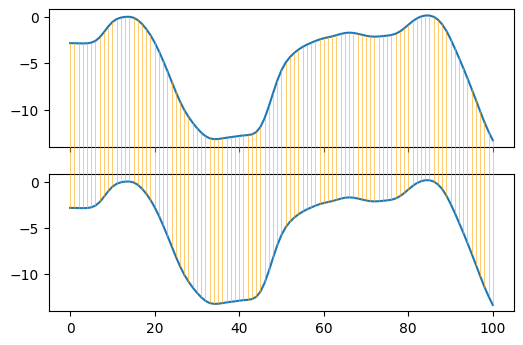
\includegraphics[width=0.99\textwidth]{machine-learning/warping_lines_1_curve.png}
        \caption{Sample-wise Euclidean distance.}
        \label{fig:ed_ex}
    \end{subfigure}
    \begin{subfigure}[b]{0.49\textwidth}
        \centering
        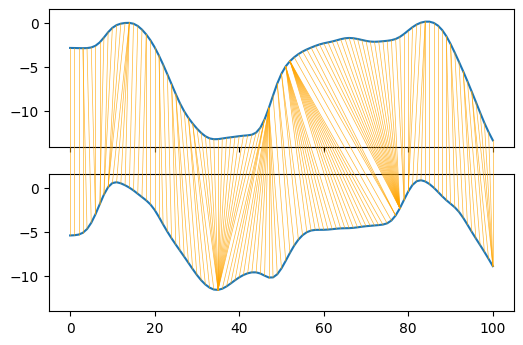
\includegraphics[width=0.99\textwidth]{machine-learning/warping_lines_2_curves.png}
        \caption{\acrshort{dtw} distance.}
        \label{fig:dtw_ex}
    \end{subfigure}
    \caption{An illustration of the difference between sample-wise Euclidean distance between time series, and \acrshort{dtw} distance between time series.}
    \label{fig:ed_dtw_ex}
\end{figure}

In the raw-data based approach to \acrshort{tsc}, choice of dissimilarity metric is paramount and is chosen based on what objective of the \acrshort{tsc} is, and the different lengths of the time series to be compared. When clustering with regard to similarity in shape, the similarity metric can be lock-step (one-to-one) or elastic (one-to-many) \cite{tsc_rev}. An example of a lock-step measure is the use of Euclidean distance to measure the distance between time series sample-wise. However, this becomes problematic when the time series are not of equal length. \acrfull{dtw} distance is a powerful alternative for Euclidean distance to measure the shape-based distance between two time series. To understand how the \acrshort{dtw} distance works as a dissimilarity metric, one can imagine that it warps one time series such that the two series are equal in length, and then measures the Euclidean distance between them. This is illustrated in figure \ref{fig:ed_dtw_ex}. \acrshort{dtw} is probably most famous from speech recognition, where it is applied to find out which phoneme\footnote{Phoneme is a term from speech recognition and refers to the largest unit of sound for which the frequency spectrum is constant. Phonemes are considered as the ''atomic sounds'' that make up speech.} in a dictionary of phonemes is the optimal fit to a recorded sound. To calculate the \acrshort{dtw} distance between two time series $x$ and $y$ of length $n$ and $m$ respectively. First an $(n \times m)$ matrix is constructed called the \acrfull{lcm}. Element $\mathrm{LCM}(i,j)$ is the sample-wise quadratic distance between $x_i$ and $y_i$ ($(x_i - y_i)^2$). The next step is to create a warping path $P = \{p_1, p_2, ..., p_L\}$ across the \acrshort{lcm}. The warping path must fulfill three conditions: the boundary condition, the continuity condition, and the monotonicity condition. 

\begin{enumerate} 
    \item \textbf{Boundary}: The path must begin and end in the corners of the \acrshort{lcm}. $p_0 = \mathrm{LCM(1,1)}$, $p_L = \mathrm{LCM(n,m)}$ 
    \item \textbf{Continuity}: Two adjacent warping steps $p_k$ and $p_{k+1}$ must be equal to adjacent elements on the \acrshort{lcm}. This means that the matrix elements that $p_k$ and $p_{k+1}$ point to, must be adjacent horizontally, vertically or diagonally in the \acrshort{lcm}.
    \item \textbf{Monotonicity}: The warping path must increase monotonically. This means that the warping path cannot go backwards index-wise. If one combines the continuity, and monotonicity constraints, and lets $p_k = \mathrm{LCM}(i,j)$, valid values for $p_k$ are $\mathrm{LCM}(i+1,j)$, $\mathrm{LCM}(i,j+1)$ and $\mathrm{LCM}(i+1,j+1)$.
\end{enumerate}

The warping distance of the warping path $P$ is the sum of the \acrshort{lcm} elements that entries of $P$ are equal to. The \acrshort{dtw} distance between time series $x$ and $y$ is then defined as the square root of the smallest possible warping distance between $x$ and $y$. The warping path corresponding to the smallest warping distance can be found by using a recurrent algorithm from dynamic programming shown in equation \eqref{eq:dp_dtw} \cite{pjotr}.

\begin{equation}
    \begin{split}
        p_1     &= \mathrm{LCM}\{ 1,1 \}, p_L = \mathrm{LCM}\{ n,m \}  \\
        p_{i}   &= \mathrm{LCM}\{ f,g \} \\
        p_{i+1} &= \mathrm{min} \left \{ \mathrm{LCM} \{ f+1,g\}, \mathrm{LCM} \{ f,g+1\}, \mathrm{LCM} \{ f+1,g+1\} \right  \}
    \end{split}
    \label{eq:dp_dtw}
\end{equation}

Although the \acrshort{dtw} distance is more flexible than estimating Euclidean distance between two time series, it comes at the cost of much higher run time and space requirements. The time complexity for calculating the dissimilarity matrix of a set of $N$ time series using the \acrshort{dtw} distance is $O\left ( n m N^{2} \right )$ \cite{tsc_rev}. An illustration of how the \acrshort{dtw} distance between two time series is estimated is shown in figure \ref{fig:warping_path}. 

\begin{figure}
    \centering
    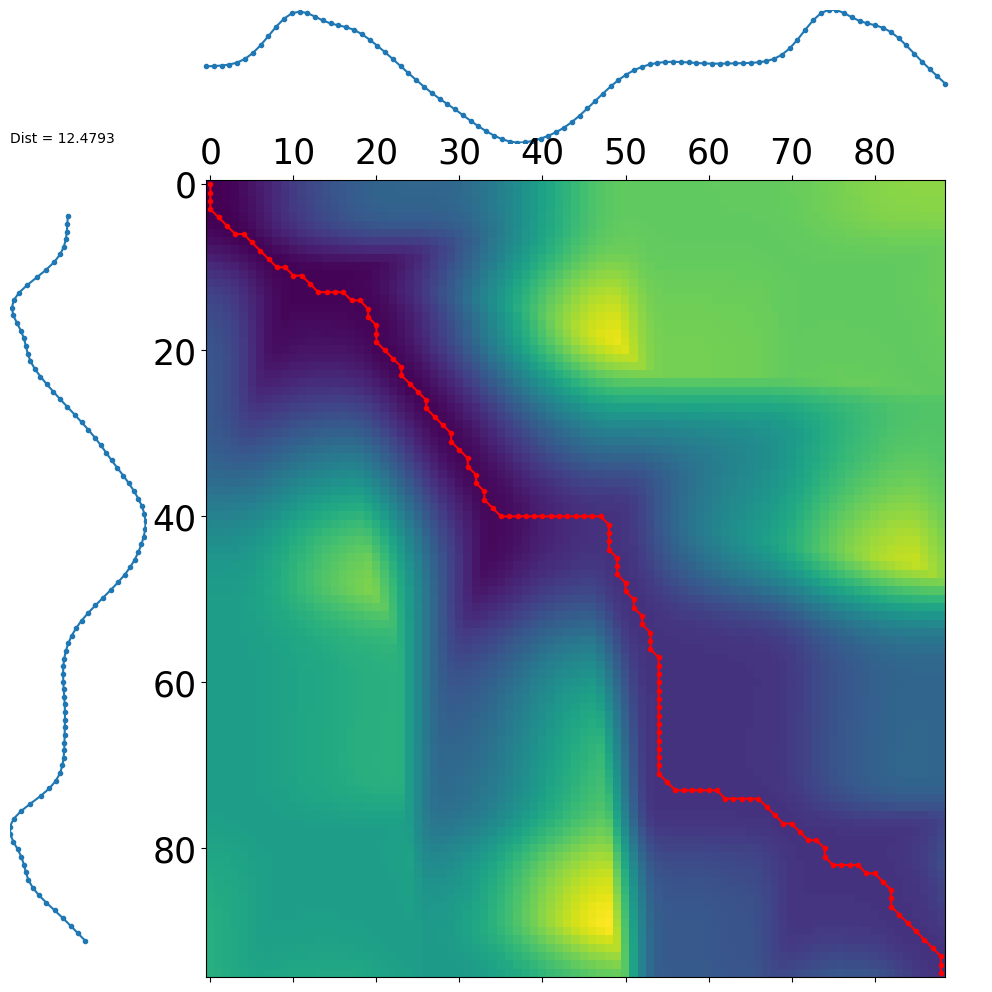
\includegraphics[width=0.49\textwidth]{machine-learning/warping_path_2_curves.png}
    \caption{An illustration of \acrshort{dtw} distance. The big coloured square is the \acrshort{lcm}, each monochromatic subsquare in is an entry in the \acrshort{lcm}. The color of each subsquare indicates the magnitude of the quadratic distance in that entry, blue indicates low, and green and yellow indicate higher values. The red line is the warping path.}
    \label{fig:warping_path}
\end{figure}

\subsection{Agglomerative Hierarchical Clustering} \label{sec:ahc}

The agglomerative hierarchical clustering algorithm is the chosen clustering algorithm in this work. It is a \textit{hard} clustering algorithm, meaning that data objects are given a single cluster assignment, and do not have partial memberships to many different clusters. Clustering algorithms that assign data objects partial memberships to many clusters are called \textit{soft} clustering algorithms. \bigskip

\textit{Partitional clustering algorithms} is a family of clustering algorithms that is an alternative to the family of hierarchical clustering algorithms. Partitional methods work iteratively and rely on defining prototypes that represent the cluster center. In the first iteration, the prototypes are randomly initialized. Then, the dissimilarity between all data objects and the prototypes are calculated, the data objects are then assigned to the cluster where the dissimilarity to the cluster prototype is minimal. The final step is to update the cluster prototypes such that they best represent the center of the new cluster. These steps repeat until the value of the cluster prototypes, and cluster membership assignments converge. \bigskip

Hierarchical clustering algorithms have two central advantages over partitional clustering algorithms, such as K-means, K-medoids, and fuzzy C-means. The first advantage is that the user does not have to decide the number of clusters they want to partition the dataset into prior to using the algorithm. The second is that due to the reliance on cluster prototypes and their random initialization, the cluster assignments yielded when the partitional algorithm are non-deterministic. The clusters assignments that a partitional algorithm converges to is dependent on what values the cluster prototypes are given upon initialization. Hierarchical clustering algorithms will always yield the same hierarchy of cluster assignments, given that the same dissimilarity matrix is inputted. \bigskip

There are two main types of hierarchical clustering algorithms, \textit{divisive} and \textit{agglomerative}. To understand the difference between these two algorithms, it helps to first understand how agglomerative hierarchical clustering works. Assume one is applying the hierarchical clustering algorithm to cluster a dataset of $N$ data objects. In the initial step, the algorithm takes the dissimilarity matrix as input, and every data object in the dataset is regarded as a separate cluster. Next, the case of $N-1$ clusters is considered, two of the existing clusters are merged based on which clusters have the lowest dissimilarity such that there then are $N-1$ clusters. The dissimilarity between clusters is estimated with what is called a \textit{linkage criterion}, which will be expanded upon later. This step of merging existing clusters is repeated until all data objects are contained in one cluster. The result is a hierarchy of clusters called a \textit{dendrogram}, that can yield cluster assignments at all the possible number of clusters. If one says that agglomerative hierarchical clustering has a bottom-top approach, divisive hierarchical clustering can be said to have a top-bottom approach. It starts at the top of the dendrogram with all data objects in one cluster and continuously splits the cluster until every object is contained in its own cluster. In this work, seven different linkage criteria are used, as detailed below.

\begin{itemize}
    \item \textbf{Single linkage}: Computes the dissimilarity between two clusters as the smallest dissimilarity between two individual members of each cluster \cite{dependency_tsc_energy_markets}.
    \item \textbf{Complete linkage}: Computes the dissimilarity between two clusters as the biggest dissimilarity between two individual members of each cluster \cite{financial_tsc_variance_ratio}.
    \item \textbf{Average linkage}: Computes the dissimilarity between two clusters as the average dissimilarity between all members of each cluster \cite{dependency_tsc_energy_markets}.
    \item \textbf{Ward linkage}: Computes the dissimilarity between two clusters as the increase in sum squared dissimilarity of the entire cluster that would be the result of merging the two clusters \cite{copula_ica_tsc}.
    \item \textbf{Centroid linkage}: Computes the dissimilarity between clusters by representing each cluster with a ''centroid'', which is another word for a cluster prototype. The dissimilarity between clusters is then computed as the dissimilarity between the centroids of each cluster. After the two clusters are merged, a new centroid is computed based on all the cluster members of the two clusters merged \cite{scipy_hier_reference}.
    \item \textbf{Median linkage}: Computes dissimilarity between two clusters in the same way as the centroid linkage, the only difference being that after the clusters are merged, the new centroid is computed as the average of the two previous centroids \cite{scipy_hier_reference}.
    \item \textbf{Weighted linkage}: Works in a method similar to the average linkage, the only difference being that after two clusters are merged, this linkage requires all the entries in the dissimilarity matrix that pertain to members of this cluster to be averaged. This merging of entries in the dissimilarity matrix reduces the number of computations required further down the line because there will be fewer dissimilarity values to average \cite{scipy_hier_reference}.
\end{itemize}

One of the apparent disadvantages of the hierarchical clustering algorithms is that they have quadratic time complexity $O(N^2)$, and have also received critique for lacking flexibility \cite{tsc_rev}. The lack of flexibility is because after two clusters are merged, they cannot be split for re-evaluation when a lower number of clusters is considered. 

\subsection{Curse of Dimensionality} \label{sec:curse_dimensionality}
The curse of dimensionality is a term used to explain the problem of having \textit{too much} information about each individual object, with regard to the number of objects that make up the dataset. This concept may sound counterintuitive, but it is a real issue in classification and regression problems. For every new parameter that is added to a data object (or every dimension that is added to a dataset), additional undesired stochastic behavior is added as well. Undesired stochastic behavior is often referred to as \textit{noise} because it makes it harder to detect the relation between the input variables and the target variable. If the amount of noise in a dataset becomes high enough, a machine learning model will become unable to generalize the relationship between the input variables and the target variables. The curse of dimensionality refers to the issue of the noise that is added when too many dimensions have been used to represent a dataset. The number of dimensions must be chosen in the context of how many objects there are in the dataset because if the number of objects in the dataset is great enough, the information added by an additional dimension could outweigh the additional noise cost.

\clearpage

\section{Artificial Neural Networks} \label{sec:ann}

This section will explain how layers of perceptrons form an \acrfull{ann}, how the said network is trained, the function of convolutional and recurrent layers in an \acrshort{ann}, and will discuss the challenges of underfitting and overfitting.

\subsection{Multi-layer Perceptrons} \label{sec:mlp}
Figure \ref{fig:perc_nn}a depicts the building blocks of an \acrshort{ann}, the perceptron. 
The perceptron is a model of an artificial neuron, it takes in $n$ inputs, performs a weighted sum of the inputs and a bias $b$, and sends the sum through what is called an activation function. A single perceptron is only able to perform binary classification on linearly separable points. However, by combining multiple perceptrons into a layer, and multiple layers of perceptrons into a \acrfull{mlp}, they can capture complex non-linear relationships. 

\begin{figure}[H]
\begin{center}
    \tikzstyle{init} = [pin edge={to-,thin,black}]
\tikzstyle{circ} = [circle, minimum size=1cm, text centered, draw=black, fill=blue!20]
\tikzstyle{arrow} = [thin,->,>=stealth]
\tikzstyle{arrow_t} = [very thin,->,>=stealth]

\tikzstyle{perc_in} = [circle, minimum size=1mm, text centered, draw=black, fill=blue!20]
\tikzstyle{perc_ou} = [circle, minimum size=1mm, text centered, draw=black, fill=red!20]
\tikzstyle{perc_hi} = [circle, minimum size=1mm, text centered, draw=black, fill=green!20]

\begin{tikzpicture}
% Perceptron
\node (x1) [init] {$x_1$};
\node (x2) [init, below of=x1] {$x_2$};
\node (vdots) [init, below of=x2] {$\vdots$};
\node (xn) [init, below of=vdots] {$x_n$};

\node (sum) [circ, right of=x2, xshift=0.7cm, yshift=-5mm] {$\sum$};
\node (b) [init, below of=sum, yshift=-0.7cm] {$b$};
\node (obj) [circ, right of=sum, xshift=1cm] {$f(\cdot)$};
\node (output) [init, right of=obj, xshift=0.7cm] {};

\draw [arrow] (x1) --node[anchor=north] {$w_1$} (sum);
\draw [arrow] (x2) --node[anchor=north] {$w_2$} (sum);
\draw [arrow] (xn) --node[anchor=west] {$w_n$} (sum);
\draw [arrow] (b) --node[anchor=west] {$w_b$} (sum);
\draw [arrow] (sum) -- (obj);
\draw [arrow] (obj) -- (output);

% ANN
\node (i2) [init, right of=output] {$x_2$};
\node (i1) [init,, above of=i2] {$x_1$};
\node (i3) [init, below of=i2] {$x_3$};

\node (in0) [perc_in, right of=i1] {};
\node (in1) [perc_in, below of=in0] {};
\node (in2) [perc_in, below of=in1] {};

\node (hi0) [perc_hi, right of=in0, yshift=3.3mm] {};
\node (hi1) [perc_hi, below of=hi0, yshift=3.3mm] {};
\node (hi2) [perc_hi, below of=hi1, yshift=3.3mm] {};
\node (hi3) [perc_hi, below of=hi2, yshift=3.3mm] {};
\node (hi4) [perc_hi, below of=hi3, yshift=3.3mm] {};

\node (ou0) [perc_ou, right of=hi2] {};

\draw [arrow_t] (i1) -- (in0);
\draw [arrow_t] (i1) -- (in1);
\draw [arrow_t] (i1) -- (in2);
\draw [arrow_t] (i2) -- (in0);
\draw [arrow_t] (i2) -- (in1);
\draw [arrow_t] (i2) -- (in2);
\draw [arrow_t] (i3) -- (in0);
\draw [arrow_t] (i3) -- (in1);
\draw [arrow_t] (i3) -- (in2);

\draw [arrow_t] (in0) -- (hi0);
\draw [arrow_t] (in0) -- (hi1);
\draw [arrow_t] (in0) -- (hi2);
\draw [arrow_t] (in0) -- (hi3);
\draw [arrow_t] (in0) -- (hi4);
\draw [arrow_t] (in1) -- (hi0);
\draw [arrow_t] (in1) -- (hi1);
\draw [arrow_t] (in1) -- (hi2);
\draw [arrow_t] (in1) -- (hi3);
\draw [arrow_t] (in1) -- (hi4);
\draw [arrow_t] (in2) -- (hi0);
\draw [arrow_t] (in2) -- (hi1);
\draw [arrow_t] (in2) -- (hi2);
\draw [arrow_t] (in2) -- (hi3);
\draw [arrow_t] (in2) -- (hi4);

\draw [arrow_t] (hi0) -- (ou0);
\draw [arrow_t] (hi1) -- (ou0);
\draw [arrow_t] (hi2) -- (ou0);
\draw [arrow_t] (hi3) -- (ou0);
\draw [arrow_t] (hi4) -- (ou0);

\node (label_a) [init, below of=b] {$(a)$};
\node (label_a) [init, right of=label_a, xshift=5cm] {$(b)$};
\end{tikzpicture}
\end{center}
\caption{$(a)$ A Perceptron. $(b)$ Example of a simple \acrshort{ann} known as an \acrshort{mlp}.} 
\label{fig:perc_nn}
\end{figure}

\begin{equation}
    O(\mathbf{x}) = f \left ( \sum_{i = 1}^N w_i x_i + w_b b\right )
    \label{eq:perc}
\end{equation}

Equation \eqref{eq:perc} shows what the output of a perceptron ($O(\mathbf{x})$) is in terms of its weights $\{w_i\}$, the input $\mathbf{x}$, its activation function $f(\cdot)$ and its bias $b$. The purpose of an activation function is to give each perceptron the ability to perform actions that are not purely linear on its inputs \cite{dl_book}. Consider that the absence of an activation function, all a perceptron is doing is outputting a weighted sum of its inputs. Any continuous function can, in principle, be used as an activation function, but some functions are more common than others. Figure \ref{fig:obj_funcs} shows the three most popular activation functions used in modern \acrshort{ann}, the sigmoid function, $\mathrm{tanh}$ function, and \acrfull{relu}. The sigmoid function was one of the first activation functions introduced, and it shares many similar characteristics with the $\mathrm{tanh}$ function. The sigmoid, and $\mathrm{tanh}$ functions are both hyperbolic functions that grant non-linear properties to the perceptron. However, the \acrshort{relu} function is often preferred over the two former functions for two important reasons. First, the hyperbolic functions suffer an issue of saturation when the weighted sums of the input becomes sufficiently large, while the \acrshort{relu} does not. The second reason is not as technical, but is still important. Since an \acrshort{ann} can be made up of hundreds, or even thousands of perceptrons, the computation of complex exponential functions for every unit is computationally expensive, whereas the computation of the \acrshort{relu} is significantly less so. 

\begin{figure}[H]
    \centering
    \begin{subfigure}[b]{0.32\textwidth}
        \centering
        %% Creator: Matplotlib, PGF backend
%%
%% To include the figure in your LaTeX document, write
%%   \input{<filename>.pgf}
%%
%% Make sure the required packages are loaded in your preamble
%%   \usepackage{pgf}
%%
%% Figures using additional raster images can only be included by \input if
%% they are in the same directory as the main LaTeX file. For loading figures
%% from other directories you can use the `import` package
%%   \usepackage{import}
%% and then include the figures with
%%   \import{<path to file>}{<filename>.pgf}
%%
%% Matplotlib used the following preamble
%%
\begingroup%
\makeatletter%
\begin{pgfpicture}%
\pgfpathrectangle{\pgfpointorigin}{\pgfqpoint{1.900000in}{1.900000in}}%
\pgfusepath{use as bounding box, clip}%
\begin{pgfscope}%
\pgfsetbuttcap%
\pgfsetmiterjoin%
\definecolor{currentfill}{rgb}{1.000000,1.000000,1.000000}%
\pgfsetfillcolor{currentfill}%
\pgfsetlinewidth{0.000000pt}%
\definecolor{currentstroke}{rgb}{1.000000,1.000000,1.000000}%
\pgfsetstrokecolor{currentstroke}%
\pgfsetdash{}{0pt}%
\pgfpathmoveto{\pgfqpoint{0.000000in}{0.000000in}}%
\pgfpathlineto{\pgfqpoint{1.900000in}{0.000000in}}%
\pgfpathlineto{\pgfqpoint{1.900000in}{1.900000in}}%
\pgfpathlineto{\pgfqpoint{0.000000in}{1.900000in}}%
\pgfpathclose%
\pgfusepath{fill}%
\end{pgfscope}%
\begin{pgfscope}%
\pgfsetbuttcap%
\pgfsetmiterjoin%
\definecolor{currentfill}{rgb}{1.000000,1.000000,1.000000}%
\pgfsetfillcolor{currentfill}%
\pgfsetlinewidth{0.000000pt}%
\definecolor{currentstroke}{rgb}{0.000000,0.000000,0.000000}%
\pgfsetstrokecolor{currentstroke}%
\pgfsetstrokeopacity{0.000000}%
\pgfsetdash{}{0pt}%
\pgfpathmoveto{\pgfqpoint{0.461302in}{0.308333in}}%
\pgfpathlineto{\pgfqpoint{1.800000in}{0.308333in}}%
\pgfpathlineto{\pgfqpoint{1.800000in}{1.800000in}}%
\pgfpathlineto{\pgfqpoint{0.461302in}{1.800000in}}%
\pgfpathclose%
\pgfusepath{fill}%
\end{pgfscope}%
\begin{pgfscope}%
\pgfsetbuttcap%
\pgfsetroundjoin%
\definecolor{currentfill}{rgb}{0.000000,0.000000,0.000000}%
\pgfsetfillcolor{currentfill}%
\pgfsetlinewidth{0.803000pt}%
\definecolor{currentstroke}{rgb}{0.000000,0.000000,0.000000}%
\pgfsetstrokecolor{currentstroke}%
\pgfsetdash{}{0pt}%
\pgfsys@defobject{currentmarker}{\pgfqpoint{0.000000in}{-0.048611in}}{\pgfqpoint{0.000000in}{0.000000in}}{%
\pgfpathmoveto{\pgfqpoint{0.000000in}{0.000000in}}%
\pgfpathlineto{\pgfqpoint{0.000000in}{-0.048611in}}%
\pgfusepath{stroke,fill}%
}%
\begin{pgfscope}%
\pgfsys@transformshift{0.522152in}{0.308333in}%
\pgfsys@useobject{currentmarker}{}%
\end{pgfscope}%
\end{pgfscope}%
\begin{pgfscope}%
\definecolor{textcolor}{rgb}{0.000000,0.000000,0.000000}%
\pgfsetstrokecolor{textcolor}%
\pgfsetfillcolor{textcolor}%
\pgftext[x=0.522152in,y=0.211111in,,top]{\color{textcolor}\rmfamily\fontsize{9.000000}{10.800000}\selectfont \(\displaystyle -5\)}%
\end{pgfscope}%
\begin{pgfscope}%
\pgfsetbuttcap%
\pgfsetroundjoin%
\definecolor{currentfill}{rgb}{0.000000,0.000000,0.000000}%
\pgfsetfillcolor{currentfill}%
\pgfsetlinewidth{0.803000pt}%
\definecolor{currentstroke}{rgb}{0.000000,0.000000,0.000000}%
\pgfsetstrokecolor{currentstroke}%
\pgfsetdash{}{0pt}%
\pgfsys@defobject{currentmarker}{\pgfqpoint{0.000000in}{-0.048611in}}{\pgfqpoint{0.000000in}{0.000000in}}{%
\pgfpathmoveto{\pgfqpoint{0.000000in}{0.000000in}}%
\pgfpathlineto{\pgfqpoint{0.000000in}{-0.048611in}}%
\pgfusepath{stroke,fill}%
}%
\begin{pgfscope}%
\pgfsys@transformshift{1.130651in}{0.308333in}%
\pgfsys@useobject{currentmarker}{}%
\end{pgfscope}%
\end{pgfscope}%
\begin{pgfscope}%
\definecolor{textcolor}{rgb}{0.000000,0.000000,0.000000}%
\pgfsetstrokecolor{textcolor}%
\pgfsetfillcolor{textcolor}%
\pgftext[x=1.130651in,y=0.211111in,,top]{\color{textcolor}\rmfamily\fontsize{9.000000}{10.800000}\selectfont \(\displaystyle 0\)}%
\end{pgfscope}%
\begin{pgfscope}%
\pgfsetbuttcap%
\pgfsetroundjoin%
\definecolor{currentfill}{rgb}{0.000000,0.000000,0.000000}%
\pgfsetfillcolor{currentfill}%
\pgfsetlinewidth{0.803000pt}%
\definecolor{currentstroke}{rgb}{0.000000,0.000000,0.000000}%
\pgfsetstrokecolor{currentstroke}%
\pgfsetdash{}{0pt}%
\pgfsys@defobject{currentmarker}{\pgfqpoint{0.000000in}{-0.048611in}}{\pgfqpoint{0.000000in}{0.000000in}}{%
\pgfpathmoveto{\pgfqpoint{0.000000in}{0.000000in}}%
\pgfpathlineto{\pgfqpoint{0.000000in}{-0.048611in}}%
\pgfusepath{stroke,fill}%
}%
\begin{pgfscope}%
\pgfsys@transformshift{1.739150in}{0.308333in}%
\pgfsys@useobject{currentmarker}{}%
\end{pgfscope}%
\end{pgfscope}%
\begin{pgfscope}%
\definecolor{textcolor}{rgb}{0.000000,0.000000,0.000000}%
\pgfsetstrokecolor{textcolor}%
\pgfsetfillcolor{textcolor}%
\pgftext[x=1.739150in,y=0.211111in,,top]{\color{textcolor}\rmfamily\fontsize{9.000000}{10.800000}\selectfont \(\displaystyle 5\)}%
\end{pgfscope}%
\begin{pgfscope}%
\pgfsetbuttcap%
\pgfsetroundjoin%
\definecolor{currentfill}{rgb}{0.000000,0.000000,0.000000}%
\pgfsetfillcolor{currentfill}%
\pgfsetlinewidth{0.803000pt}%
\definecolor{currentstroke}{rgb}{0.000000,0.000000,0.000000}%
\pgfsetstrokecolor{currentstroke}%
\pgfsetdash{}{0pt}%
\pgfsys@defobject{currentmarker}{\pgfqpoint{-0.048611in}{0.000000in}}{\pgfqpoint{0.000000in}{0.000000in}}{%
\pgfpathmoveto{\pgfqpoint{0.000000in}{0.000000in}}%
\pgfpathlineto{\pgfqpoint{-0.048611in}{0.000000in}}%
\pgfusepath{stroke,fill}%
}%
\begin{pgfscope}%
\pgfsys@transformshift{0.461302in}{0.376136in}%
\pgfsys@useobject{currentmarker}{}%
\end{pgfscope}%
\end{pgfscope}%
\begin{pgfscope}%
\definecolor{textcolor}{rgb}{0.000000,0.000000,0.000000}%
\pgfsetstrokecolor{textcolor}%
\pgfsetfillcolor{textcolor}%
\pgftext[x=0.100000in,y=0.332734in,left,base]{\color{textcolor}\rmfamily\fontsize{9.000000}{10.800000}\selectfont \(\displaystyle -1.0\)}%
\end{pgfscope}%
\begin{pgfscope}%
\pgfsetbuttcap%
\pgfsetroundjoin%
\definecolor{currentfill}{rgb}{0.000000,0.000000,0.000000}%
\pgfsetfillcolor{currentfill}%
\pgfsetlinewidth{0.803000pt}%
\definecolor{currentstroke}{rgb}{0.000000,0.000000,0.000000}%
\pgfsetstrokecolor{currentstroke}%
\pgfsetdash{}{0pt}%
\pgfsys@defobject{currentmarker}{\pgfqpoint{-0.048611in}{0.000000in}}{\pgfqpoint{0.000000in}{0.000000in}}{%
\pgfpathmoveto{\pgfqpoint{0.000000in}{0.000000in}}%
\pgfpathlineto{\pgfqpoint{-0.048611in}{0.000000in}}%
\pgfusepath{stroke,fill}%
}%
\begin{pgfscope}%
\pgfsys@transformshift{0.461302in}{0.715152in}%
\pgfsys@useobject{currentmarker}{}%
\end{pgfscope}%
\end{pgfscope}%
\begin{pgfscope}%
\definecolor{textcolor}{rgb}{0.000000,0.000000,0.000000}%
\pgfsetstrokecolor{textcolor}%
\pgfsetfillcolor{textcolor}%
\pgftext[x=0.100000in,y=0.671749in,left,base]{\color{textcolor}\rmfamily\fontsize{9.000000}{10.800000}\selectfont \(\displaystyle -0.5\)}%
\end{pgfscope}%
\begin{pgfscope}%
\pgfsetbuttcap%
\pgfsetroundjoin%
\definecolor{currentfill}{rgb}{0.000000,0.000000,0.000000}%
\pgfsetfillcolor{currentfill}%
\pgfsetlinewidth{0.803000pt}%
\definecolor{currentstroke}{rgb}{0.000000,0.000000,0.000000}%
\pgfsetstrokecolor{currentstroke}%
\pgfsetdash{}{0pt}%
\pgfsys@defobject{currentmarker}{\pgfqpoint{-0.048611in}{0.000000in}}{\pgfqpoint{0.000000in}{0.000000in}}{%
\pgfpathmoveto{\pgfqpoint{0.000000in}{0.000000in}}%
\pgfpathlineto{\pgfqpoint{-0.048611in}{0.000000in}}%
\pgfusepath{stroke,fill}%
}%
\begin{pgfscope}%
\pgfsys@transformshift{0.461302in}{1.054167in}%
\pgfsys@useobject{currentmarker}{}%
\end{pgfscope}%
\end{pgfscope}%
\begin{pgfscope}%
\definecolor{textcolor}{rgb}{0.000000,0.000000,0.000000}%
\pgfsetstrokecolor{textcolor}%
\pgfsetfillcolor{textcolor}%
\pgftext[x=0.199922in,y=1.010764in,left,base]{\color{textcolor}\rmfamily\fontsize{9.000000}{10.800000}\selectfont \(\displaystyle 0.0\)}%
\end{pgfscope}%
\begin{pgfscope}%
\pgfsetbuttcap%
\pgfsetroundjoin%
\definecolor{currentfill}{rgb}{0.000000,0.000000,0.000000}%
\pgfsetfillcolor{currentfill}%
\pgfsetlinewidth{0.803000pt}%
\definecolor{currentstroke}{rgb}{0.000000,0.000000,0.000000}%
\pgfsetstrokecolor{currentstroke}%
\pgfsetdash{}{0pt}%
\pgfsys@defobject{currentmarker}{\pgfqpoint{-0.048611in}{0.000000in}}{\pgfqpoint{0.000000in}{0.000000in}}{%
\pgfpathmoveto{\pgfqpoint{0.000000in}{0.000000in}}%
\pgfpathlineto{\pgfqpoint{-0.048611in}{0.000000in}}%
\pgfusepath{stroke,fill}%
}%
\begin{pgfscope}%
\pgfsys@transformshift{0.461302in}{1.393182in}%
\pgfsys@useobject{currentmarker}{}%
\end{pgfscope}%
\end{pgfscope}%
\begin{pgfscope}%
\definecolor{textcolor}{rgb}{0.000000,0.000000,0.000000}%
\pgfsetstrokecolor{textcolor}%
\pgfsetfillcolor{textcolor}%
\pgftext[x=0.199922in,y=1.349779in,left,base]{\color{textcolor}\rmfamily\fontsize{9.000000}{10.800000}\selectfont \(\displaystyle 0.5\)}%
\end{pgfscope}%
\begin{pgfscope}%
\pgfsetbuttcap%
\pgfsetroundjoin%
\definecolor{currentfill}{rgb}{0.000000,0.000000,0.000000}%
\pgfsetfillcolor{currentfill}%
\pgfsetlinewidth{0.803000pt}%
\definecolor{currentstroke}{rgb}{0.000000,0.000000,0.000000}%
\pgfsetstrokecolor{currentstroke}%
\pgfsetdash{}{0pt}%
\pgfsys@defobject{currentmarker}{\pgfqpoint{-0.048611in}{0.000000in}}{\pgfqpoint{0.000000in}{0.000000in}}{%
\pgfpathmoveto{\pgfqpoint{0.000000in}{0.000000in}}%
\pgfpathlineto{\pgfqpoint{-0.048611in}{0.000000in}}%
\pgfusepath{stroke,fill}%
}%
\begin{pgfscope}%
\pgfsys@transformshift{0.461302in}{1.732197in}%
\pgfsys@useobject{currentmarker}{}%
\end{pgfscope}%
\end{pgfscope}%
\begin{pgfscope}%
\definecolor{textcolor}{rgb}{0.000000,0.000000,0.000000}%
\pgfsetstrokecolor{textcolor}%
\pgfsetfillcolor{textcolor}%
\pgftext[x=0.199922in,y=1.688794in,left,base]{\color{textcolor}\rmfamily\fontsize{9.000000}{10.800000}\selectfont \(\displaystyle 1.0\)}%
\end{pgfscope}%
\begin{pgfscope}%
\pgfpathrectangle{\pgfqpoint{0.461302in}{0.308333in}}{\pgfqpoint{1.338698in}{1.491667in}}%
\pgfusepath{clip}%
\pgfsetrectcap%
\pgfsetroundjoin%
\pgfsetlinewidth{1.505625pt}%
\definecolor{currentstroke}{rgb}{0.121569,0.466667,0.705882}%
\pgfsetstrokecolor{currentstroke}%
\pgfsetdash{}{0pt}%
\pgfpathmoveto{\pgfqpoint{0.522152in}{1.058705in}}%
\pgfpathlineto{\pgfqpoint{0.601655in}{1.062834in}}%
\pgfpathlineto{\pgfqpoint{0.656695in}{1.067692in}}%
\pgfpathlineto{\pgfqpoint{0.705619in}{1.074187in}}%
\pgfpathlineto{\pgfqpoint{0.748428in}{1.082277in}}%
\pgfpathlineto{\pgfqpoint{0.785122in}{1.091623in}}%
\pgfpathlineto{\pgfqpoint{0.815699in}{1.101574in}}%
\pgfpathlineto{\pgfqpoint{0.846277in}{1.113922in}}%
\pgfpathlineto{\pgfqpoint{0.876855in}{1.129103in}}%
\pgfpathlineto{\pgfqpoint{0.901317in}{1.143587in}}%
\pgfpathlineto{\pgfqpoint{0.925780in}{1.160376in}}%
\pgfpathlineto{\pgfqpoint{0.950242in}{1.179645in}}%
\pgfpathlineto{\pgfqpoint{0.974704in}{1.201510in}}%
\pgfpathlineto{\pgfqpoint{0.999166in}{1.226000in}}%
\pgfpathlineto{\pgfqpoint{1.029744in}{1.260170in}}%
\pgfpathlineto{\pgfqpoint{1.060322in}{1.297863in}}%
\pgfpathlineto{\pgfqpoint{1.097015in}{1.346629in}}%
\pgfpathlineto{\pgfqpoint{1.207096in}{1.496288in}}%
\pgfpathlineto{\pgfqpoint{1.237674in}{1.533329in}}%
\pgfpathlineto{\pgfqpoint{1.268251in}{1.566730in}}%
\pgfpathlineto{\pgfqpoint{1.292714in}{1.590566in}}%
\pgfpathlineto{\pgfqpoint{1.317176in}{1.611776in}}%
\pgfpathlineto{\pgfqpoint{1.341638in}{1.630412in}}%
\pgfpathlineto{\pgfqpoint{1.366100in}{1.646606in}}%
\pgfpathlineto{\pgfqpoint{1.390563in}{1.660545in}}%
\pgfpathlineto{\pgfqpoint{1.421141in}{1.675124in}}%
\pgfpathlineto{\pgfqpoint{1.451718in}{1.686958in}}%
\pgfpathlineto{\pgfqpoint{1.482296in}{1.696480in}}%
\pgfpathlineto{\pgfqpoint{1.518990in}{1.705410in}}%
\pgfpathlineto{\pgfqpoint{1.561799in}{1.713130in}}%
\pgfpathlineto{\pgfqpoint{1.610723in}{1.719322in}}%
\pgfpathlineto{\pgfqpoint{1.665763in}{1.723949in}}%
\pgfpathlineto{\pgfqpoint{1.739150in}{1.727659in}}%
\pgfpathlineto{\pgfqpoint{1.739150in}{1.727659in}}%
\pgfusepath{stroke}%
\end{pgfscope}%
\begin{pgfscope}%
\pgfsetrectcap%
\pgfsetmiterjoin%
\pgfsetlinewidth{0.803000pt}%
\definecolor{currentstroke}{rgb}{0.000000,0.000000,0.000000}%
\pgfsetstrokecolor{currentstroke}%
\pgfsetdash{}{0pt}%
\pgfpathmoveto{\pgfqpoint{0.461302in}{0.308333in}}%
\pgfpathlineto{\pgfqpoint{0.461302in}{1.800000in}}%
\pgfusepath{stroke}%
\end{pgfscope}%
\begin{pgfscope}%
\pgfsetrectcap%
\pgfsetmiterjoin%
\pgfsetlinewidth{0.803000pt}%
\definecolor{currentstroke}{rgb}{0.000000,0.000000,0.000000}%
\pgfsetstrokecolor{currentstroke}%
\pgfsetdash{}{0pt}%
\pgfpathmoveto{\pgfqpoint{1.800000in}{0.308333in}}%
\pgfpathlineto{\pgfqpoint{1.800000in}{1.800000in}}%
\pgfusepath{stroke}%
\end{pgfscope}%
\begin{pgfscope}%
\pgfsetrectcap%
\pgfsetmiterjoin%
\pgfsetlinewidth{0.803000pt}%
\definecolor{currentstroke}{rgb}{0.000000,0.000000,0.000000}%
\pgfsetstrokecolor{currentstroke}%
\pgfsetdash{}{0pt}%
\pgfpathmoveto{\pgfqpoint{0.461302in}{0.308333in}}%
\pgfpathlineto{\pgfqpoint{1.800000in}{0.308333in}}%
\pgfusepath{stroke}%
\end{pgfscope}%
\begin{pgfscope}%
\pgfsetrectcap%
\pgfsetmiterjoin%
\pgfsetlinewidth{0.803000pt}%
\definecolor{currentstroke}{rgb}{0.000000,0.000000,0.000000}%
\pgfsetstrokecolor{currentstroke}%
\pgfsetdash{}{0pt}%
\pgfpathmoveto{\pgfqpoint{0.461302in}{1.800000in}}%
\pgfpathlineto{\pgfqpoint{1.800000in}{1.800000in}}%
\pgfusepath{stroke}%
\end{pgfscope}%
\end{pgfpicture}%
\makeatother%
\endgroup%

        \caption{$\mathrm{sigmoid}(x) = \frac{1}{1+e^{-x}}$}
        \label{fig:sigmoid}
    \end{subfigure}
    \begin{subfigure}[b]{0.32\textwidth}
        \centering
        %% Creator: Matplotlib, PGF backend
%%
%% To include the figure in your LaTeX document, write
%%   \input{<filename>.pgf}
%%
%% Make sure the required packages are loaded in your preamble
%%   \usepackage{pgf}
%%
%% Figures using additional raster images can only be included by \input if
%% they are in the same directory as the main LaTeX file. For loading figures
%% from other directories you can use the `import` package
%%   \usepackage{import}
%% and then include the figures with
%%   \import{<path to file>}{<filename>.pgf}
%%
%% Matplotlib used the following preamble
%%
\begingroup%
\makeatletter%
\begin{pgfpicture}%
\pgfpathrectangle{\pgfpointorigin}{\pgfqpoint{1.900000in}{1.900000in}}%
\pgfusepath{use as bounding box, clip}%
\begin{pgfscope}%
\pgfsetbuttcap%
\pgfsetmiterjoin%
\definecolor{currentfill}{rgb}{1.000000,1.000000,1.000000}%
\pgfsetfillcolor{currentfill}%
\pgfsetlinewidth{0.000000pt}%
\definecolor{currentstroke}{rgb}{1.000000,1.000000,1.000000}%
\pgfsetstrokecolor{currentstroke}%
\pgfsetdash{}{0pt}%
\pgfpathmoveto{\pgfqpoint{0.000000in}{0.000000in}}%
\pgfpathlineto{\pgfqpoint{1.900000in}{0.000000in}}%
\pgfpathlineto{\pgfqpoint{1.900000in}{1.900000in}}%
\pgfpathlineto{\pgfqpoint{0.000000in}{1.900000in}}%
\pgfpathclose%
\pgfusepath{fill}%
\end{pgfscope}%
\begin{pgfscope}%
\pgfsetbuttcap%
\pgfsetmiterjoin%
\definecolor{currentfill}{rgb}{1.000000,1.000000,1.000000}%
\pgfsetfillcolor{currentfill}%
\pgfsetlinewidth{0.000000pt}%
\definecolor{currentstroke}{rgb}{0.000000,0.000000,0.000000}%
\pgfsetstrokecolor{currentstroke}%
\pgfsetstrokeopacity{0.000000}%
\pgfsetdash{}{0pt}%
\pgfpathmoveto{\pgfqpoint{0.461302in}{0.308333in}}%
\pgfpathlineto{\pgfqpoint{1.800000in}{0.308333in}}%
\pgfpathlineto{\pgfqpoint{1.800000in}{1.800000in}}%
\pgfpathlineto{\pgfqpoint{0.461302in}{1.800000in}}%
\pgfpathclose%
\pgfusepath{fill}%
\end{pgfscope}%
\begin{pgfscope}%
\pgfsetbuttcap%
\pgfsetroundjoin%
\definecolor{currentfill}{rgb}{0.000000,0.000000,0.000000}%
\pgfsetfillcolor{currentfill}%
\pgfsetlinewidth{0.803000pt}%
\definecolor{currentstroke}{rgb}{0.000000,0.000000,0.000000}%
\pgfsetstrokecolor{currentstroke}%
\pgfsetdash{}{0pt}%
\pgfsys@defobject{currentmarker}{\pgfqpoint{0.000000in}{-0.048611in}}{\pgfqpoint{0.000000in}{0.000000in}}{%
\pgfpathmoveto{\pgfqpoint{0.000000in}{0.000000in}}%
\pgfpathlineto{\pgfqpoint{0.000000in}{-0.048611in}}%
\pgfusepath{stroke,fill}%
}%
\begin{pgfscope}%
\pgfsys@transformshift{0.522152in}{0.308333in}%
\pgfsys@useobject{currentmarker}{}%
\end{pgfscope}%
\end{pgfscope}%
\begin{pgfscope}%
\definecolor{textcolor}{rgb}{0.000000,0.000000,0.000000}%
\pgfsetstrokecolor{textcolor}%
\pgfsetfillcolor{textcolor}%
\pgftext[x=0.522152in,y=0.211111in,,top]{\color{textcolor}\rmfamily\fontsize{9.000000}{10.800000}\selectfont \(\displaystyle -5\)}%
\end{pgfscope}%
\begin{pgfscope}%
\pgfsetbuttcap%
\pgfsetroundjoin%
\definecolor{currentfill}{rgb}{0.000000,0.000000,0.000000}%
\pgfsetfillcolor{currentfill}%
\pgfsetlinewidth{0.803000pt}%
\definecolor{currentstroke}{rgb}{0.000000,0.000000,0.000000}%
\pgfsetstrokecolor{currentstroke}%
\pgfsetdash{}{0pt}%
\pgfsys@defobject{currentmarker}{\pgfqpoint{0.000000in}{-0.048611in}}{\pgfqpoint{0.000000in}{0.000000in}}{%
\pgfpathmoveto{\pgfqpoint{0.000000in}{0.000000in}}%
\pgfpathlineto{\pgfqpoint{0.000000in}{-0.048611in}}%
\pgfusepath{stroke,fill}%
}%
\begin{pgfscope}%
\pgfsys@transformshift{1.130651in}{0.308333in}%
\pgfsys@useobject{currentmarker}{}%
\end{pgfscope}%
\end{pgfscope}%
\begin{pgfscope}%
\definecolor{textcolor}{rgb}{0.000000,0.000000,0.000000}%
\pgfsetstrokecolor{textcolor}%
\pgfsetfillcolor{textcolor}%
\pgftext[x=1.130651in,y=0.211111in,,top]{\color{textcolor}\rmfamily\fontsize{9.000000}{10.800000}\selectfont \(\displaystyle 0\)}%
\end{pgfscope}%
\begin{pgfscope}%
\pgfsetbuttcap%
\pgfsetroundjoin%
\definecolor{currentfill}{rgb}{0.000000,0.000000,0.000000}%
\pgfsetfillcolor{currentfill}%
\pgfsetlinewidth{0.803000pt}%
\definecolor{currentstroke}{rgb}{0.000000,0.000000,0.000000}%
\pgfsetstrokecolor{currentstroke}%
\pgfsetdash{}{0pt}%
\pgfsys@defobject{currentmarker}{\pgfqpoint{0.000000in}{-0.048611in}}{\pgfqpoint{0.000000in}{0.000000in}}{%
\pgfpathmoveto{\pgfqpoint{0.000000in}{0.000000in}}%
\pgfpathlineto{\pgfqpoint{0.000000in}{-0.048611in}}%
\pgfusepath{stroke,fill}%
}%
\begin{pgfscope}%
\pgfsys@transformshift{1.739150in}{0.308333in}%
\pgfsys@useobject{currentmarker}{}%
\end{pgfscope}%
\end{pgfscope}%
\begin{pgfscope}%
\definecolor{textcolor}{rgb}{0.000000,0.000000,0.000000}%
\pgfsetstrokecolor{textcolor}%
\pgfsetfillcolor{textcolor}%
\pgftext[x=1.739150in,y=0.211111in,,top]{\color{textcolor}\rmfamily\fontsize{9.000000}{10.800000}\selectfont \(\displaystyle 5\)}%
\end{pgfscope}%
\begin{pgfscope}%
\pgfsetbuttcap%
\pgfsetroundjoin%
\definecolor{currentfill}{rgb}{0.000000,0.000000,0.000000}%
\pgfsetfillcolor{currentfill}%
\pgfsetlinewidth{0.803000pt}%
\definecolor{currentstroke}{rgb}{0.000000,0.000000,0.000000}%
\pgfsetstrokecolor{currentstroke}%
\pgfsetdash{}{0pt}%
\pgfsys@defobject{currentmarker}{\pgfqpoint{-0.048611in}{0.000000in}}{\pgfqpoint{0.000000in}{0.000000in}}{%
\pgfpathmoveto{\pgfqpoint{0.000000in}{0.000000in}}%
\pgfpathlineto{\pgfqpoint{-0.048611in}{0.000000in}}%
\pgfusepath{stroke,fill}%
}%
\begin{pgfscope}%
\pgfsys@transformshift{0.461302in}{0.376136in}%
\pgfsys@useobject{currentmarker}{}%
\end{pgfscope}%
\end{pgfscope}%
\begin{pgfscope}%
\definecolor{textcolor}{rgb}{0.000000,0.000000,0.000000}%
\pgfsetstrokecolor{textcolor}%
\pgfsetfillcolor{textcolor}%
\pgftext[x=0.100000in,y=0.332734in,left,base]{\color{textcolor}\rmfamily\fontsize{9.000000}{10.800000}\selectfont \(\displaystyle -1.0\)}%
\end{pgfscope}%
\begin{pgfscope}%
\pgfsetbuttcap%
\pgfsetroundjoin%
\definecolor{currentfill}{rgb}{0.000000,0.000000,0.000000}%
\pgfsetfillcolor{currentfill}%
\pgfsetlinewidth{0.803000pt}%
\definecolor{currentstroke}{rgb}{0.000000,0.000000,0.000000}%
\pgfsetstrokecolor{currentstroke}%
\pgfsetdash{}{0pt}%
\pgfsys@defobject{currentmarker}{\pgfqpoint{-0.048611in}{0.000000in}}{\pgfqpoint{0.000000in}{0.000000in}}{%
\pgfpathmoveto{\pgfqpoint{0.000000in}{0.000000in}}%
\pgfpathlineto{\pgfqpoint{-0.048611in}{0.000000in}}%
\pgfusepath{stroke,fill}%
}%
\begin{pgfscope}%
\pgfsys@transformshift{0.461302in}{0.715152in}%
\pgfsys@useobject{currentmarker}{}%
\end{pgfscope}%
\end{pgfscope}%
\begin{pgfscope}%
\definecolor{textcolor}{rgb}{0.000000,0.000000,0.000000}%
\pgfsetstrokecolor{textcolor}%
\pgfsetfillcolor{textcolor}%
\pgftext[x=0.100000in,y=0.671749in,left,base]{\color{textcolor}\rmfamily\fontsize{9.000000}{10.800000}\selectfont \(\displaystyle -0.5\)}%
\end{pgfscope}%
\begin{pgfscope}%
\pgfsetbuttcap%
\pgfsetroundjoin%
\definecolor{currentfill}{rgb}{0.000000,0.000000,0.000000}%
\pgfsetfillcolor{currentfill}%
\pgfsetlinewidth{0.803000pt}%
\definecolor{currentstroke}{rgb}{0.000000,0.000000,0.000000}%
\pgfsetstrokecolor{currentstroke}%
\pgfsetdash{}{0pt}%
\pgfsys@defobject{currentmarker}{\pgfqpoint{-0.048611in}{0.000000in}}{\pgfqpoint{0.000000in}{0.000000in}}{%
\pgfpathmoveto{\pgfqpoint{0.000000in}{0.000000in}}%
\pgfpathlineto{\pgfqpoint{-0.048611in}{0.000000in}}%
\pgfusepath{stroke,fill}%
}%
\begin{pgfscope}%
\pgfsys@transformshift{0.461302in}{1.054167in}%
\pgfsys@useobject{currentmarker}{}%
\end{pgfscope}%
\end{pgfscope}%
\begin{pgfscope}%
\definecolor{textcolor}{rgb}{0.000000,0.000000,0.000000}%
\pgfsetstrokecolor{textcolor}%
\pgfsetfillcolor{textcolor}%
\pgftext[x=0.199922in,y=1.010764in,left,base]{\color{textcolor}\rmfamily\fontsize{9.000000}{10.800000}\selectfont \(\displaystyle 0.0\)}%
\end{pgfscope}%
\begin{pgfscope}%
\pgfsetbuttcap%
\pgfsetroundjoin%
\definecolor{currentfill}{rgb}{0.000000,0.000000,0.000000}%
\pgfsetfillcolor{currentfill}%
\pgfsetlinewidth{0.803000pt}%
\definecolor{currentstroke}{rgb}{0.000000,0.000000,0.000000}%
\pgfsetstrokecolor{currentstroke}%
\pgfsetdash{}{0pt}%
\pgfsys@defobject{currentmarker}{\pgfqpoint{-0.048611in}{0.000000in}}{\pgfqpoint{0.000000in}{0.000000in}}{%
\pgfpathmoveto{\pgfqpoint{0.000000in}{0.000000in}}%
\pgfpathlineto{\pgfqpoint{-0.048611in}{0.000000in}}%
\pgfusepath{stroke,fill}%
}%
\begin{pgfscope}%
\pgfsys@transformshift{0.461302in}{1.393182in}%
\pgfsys@useobject{currentmarker}{}%
\end{pgfscope}%
\end{pgfscope}%
\begin{pgfscope}%
\definecolor{textcolor}{rgb}{0.000000,0.000000,0.000000}%
\pgfsetstrokecolor{textcolor}%
\pgfsetfillcolor{textcolor}%
\pgftext[x=0.199922in,y=1.349779in,left,base]{\color{textcolor}\rmfamily\fontsize{9.000000}{10.800000}\selectfont \(\displaystyle 0.5\)}%
\end{pgfscope}%
\begin{pgfscope}%
\pgfsetbuttcap%
\pgfsetroundjoin%
\definecolor{currentfill}{rgb}{0.000000,0.000000,0.000000}%
\pgfsetfillcolor{currentfill}%
\pgfsetlinewidth{0.803000pt}%
\definecolor{currentstroke}{rgb}{0.000000,0.000000,0.000000}%
\pgfsetstrokecolor{currentstroke}%
\pgfsetdash{}{0pt}%
\pgfsys@defobject{currentmarker}{\pgfqpoint{-0.048611in}{0.000000in}}{\pgfqpoint{0.000000in}{0.000000in}}{%
\pgfpathmoveto{\pgfqpoint{0.000000in}{0.000000in}}%
\pgfpathlineto{\pgfqpoint{-0.048611in}{0.000000in}}%
\pgfusepath{stroke,fill}%
}%
\begin{pgfscope}%
\pgfsys@transformshift{0.461302in}{1.732197in}%
\pgfsys@useobject{currentmarker}{}%
\end{pgfscope}%
\end{pgfscope}%
\begin{pgfscope}%
\definecolor{textcolor}{rgb}{0.000000,0.000000,0.000000}%
\pgfsetstrokecolor{textcolor}%
\pgfsetfillcolor{textcolor}%
\pgftext[x=0.199922in,y=1.688794in,left,base]{\color{textcolor}\rmfamily\fontsize{9.000000}{10.800000}\selectfont \(\displaystyle 1.0\)}%
\end{pgfscope}%
\begin{pgfscope}%
\pgfpathrectangle{\pgfqpoint{0.461302in}{0.308333in}}{\pgfqpoint{1.338698in}{1.491667in}}%
\pgfusepath{clip}%
\pgfsetrectcap%
\pgfsetroundjoin%
\pgfsetlinewidth{1.505625pt}%
\definecolor{currentstroke}{rgb}{0.121569,0.466667,0.705882}%
\pgfsetstrokecolor{currentstroke}%
\pgfsetdash{}{0pt}%
\pgfpathmoveto{\pgfqpoint{0.522152in}{0.376198in}}%
\pgfpathlineto{\pgfqpoint{0.705619in}{0.377391in}}%
\pgfpathlineto{\pgfqpoint{0.772890in}{0.379918in}}%
\pgfpathlineto{\pgfqpoint{0.815699in}{0.383757in}}%
\pgfpathlineto{\pgfqpoint{0.846277in}{0.388686in}}%
\pgfpathlineto{\pgfqpoint{0.870739in}{0.394810in}}%
\pgfpathlineto{\pgfqpoint{0.889086in}{0.401260in}}%
\pgfpathlineto{\pgfqpoint{0.907433in}{0.409880in}}%
\pgfpathlineto{\pgfqpoint{0.925780in}{0.421359in}}%
\pgfpathlineto{\pgfqpoint{0.944126in}{0.436563in}}%
\pgfpathlineto{\pgfqpoint{0.956357in}{0.449290in}}%
\pgfpathlineto{\pgfqpoint{0.968589in}{0.464515in}}%
\pgfpathlineto{\pgfqpoint{0.980820in}{0.482645in}}%
\pgfpathlineto{\pgfqpoint{0.993051in}{0.504120in}}%
\pgfpathlineto{\pgfqpoint{1.005282in}{0.529392in}}%
\pgfpathlineto{\pgfqpoint{1.017513in}{0.558913in}}%
\pgfpathlineto{\pgfqpoint{1.029744in}{0.593095in}}%
\pgfpathlineto{\pgfqpoint{1.041975in}{0.632273in}}%
\pgfpathlineto{\pgfqpoint{1.060322in}{0.700825in}}%
\pgfpathlineto{\pgfqpoint{1.078669in}{0.780971in}}%
\pgfpathlineto{\pgfqpoint{1.097015in}{0.871401in}}%
\pgfpathlineto{\pgfqpoint{1.127593in}{1.037134in}}%
\pgfpathlineto{\pgfqpoint{1.164287in}{1.236932in}}%
\pgfpathlineto{\pgfqpoint{1.182633in}{1.327362in}}%
\pgfpathlineto{\pgfqpoint{1.200980in}{1.407508in}}%
\pgfpathlineto{\pgfqpoint{1.219327in}{1.476061in}}%
\pgfpathlineto{\pgfqpoint{1.237674in}{1.532935in}}%
\pgfpathlineto{\pgfqpoint{1.249905in}{1.564739in}}%
\pgfpathlineto{\pgfqpoint{1.262136in}{1.592081in}}%
\pgfpathlineto{\pgfqpoint{1.274367in}{1.615397in}}%
\pgfpathlineto{\pgfqpoint{1.286598in}{1.635143in}}%
\pgfpathlineto{\pgfqpoint{1.298829in}{1.651768in}}%
\pgfpathlineto{\pgfqpoint{1.311060in}{1.665695in}}%
\pgfpathlineto{\pgfqpoint{1.329407in}{1.682369in}}%
\pgfpathlineto{\pgfqpoint{1.347754in}{1.694983in}}%
\pgfpathlineto{\pgfqpoint{1.366100in}{1.704472in}}%
\pgfpathlineto{\pgfqpoint{1.384447in}{1.711579in}}%
\pgfpathlineto{\pgfqpoint{1.408909in}{1.718334in}}%
\pgfpathlineto{\pgfqpoint{1.439487in}{1.723776in}}%
\pgfpathlineto{\pgfqpoint{1.476181in}{1.727576in}}%
\pgfpathlineto{\pgfqpoint{1.525105in}{1.730125in}}%
\pgfpathlineto{\pgfqpoint{1.604608in}{1.731635in}}%
\pgfpathlineto{\pgfqpoint{1.739150in}{1.732135in}}%
\pgfpathlineto{\pgfqpoint{1.739150in}{1.732135in}}%
\pgfusepath{stroke}%
\end{pgfscope}%
\begin{pgfscope}%
\pgfsetrectcap%
\pgfsetmiterjoin%
\pgfsetlinewidth{0.803000pt}%
\definecolor{currentstroke}{rgb}{0.000000,0.000000,0.000000}%
\pgfsetstrokecolor{currentstroke}%
\pgfsetdash{}{0pt}%
\pgfpathmoveto{\pgfqpoint{0.461302in}{0.308333in}}%
\pgfpathlineto{\pgfqpoint{0.461302in}{1.800000in}}%
\pgfusepath{stroke}%
\end{pgfscope}%
\begin{pgfscope}%
\pgfsetrectcap%
\pgfsetmiterjoin%
\pgfsetlinewidth{0.803000pt}%
\definecolor{currentstroke}{rgb}{0.000000,0.000000,0.000000}%
\pgfsetstrokecolor{currentstroke}%
\pgfsetdash{}{0pt}%
\pgfpathmoveto{\pgfqpoint{1.800000in}{0.308333in}}%
\pgfpathlineto{\pgfqpoint{1.800000in}{1.800000in}}%
\pgfusepath{stroke}%
\end{pgfscope}%
\begin{pgfscope}%
\pgfsetrectcap%
\pgfsetmiterjoin%
\pgfsetlinewidth{0.803000pt}%
\definecolor{currentstroke}{rgb}{0.000000,0.000000,0.000000}%
\pgfsetstrokecolor{currentstroke}%
\pgfsetdash{}{0pt}%
\pgfpathmoveto{\pgfqpoint{0.461302in}{0.308333in}}%
\pgfpathlineto{\pgfqpoint{1.800000in}{0.308333in}}%
\pgfusepath{stroke}%
\end{pgfscope}%
\begin{pgfscope}%
\pgfsetrectcap%
\pgfsetmiterjoin%
\pgfsetlinewidth{0.803000pt}%
\definecolor{currentstroke}{rgb}{0.000000,0.000000,0.000000}%
\pgfsetstrokecolor{currentstroke}%
\pgfsetdash{}{0pt}%
\pgfpathmoveto{\pgfqpoint{0.461302in}{1.800000in}}%
\pgfpathlineto{\pgfqpoint{1.800000in}{1.800000in}}%
\pgfusepath{stroke}%
\end{pgfscope}%
\end{pgfpicture}%
\makeatother%
\endgroup%

        \caption{$\mathrm{tanh}(x) = \frac{e^{x}-e^{-x}}{e^{x}+e^{-x}}$}
        \label{fig:tanh}
    \end{subfigure}
    \begin{subfigure}[b]{0.32\textwidth}
        \centering
        %% Creator: Matplotlib, PGF backend
%%
%% To include the figure in your LaTeX document, write
%%   \input{<filename>.pgf}
%%
%% Make sure the required packages are loaded in your preamble
%%   \usepackage{pgf}
%%
%% Figures using additional raster images can only be included by \input if
%% they are in the same directory as the main LaTeX file. For loading figures
%% from other directories you can use the `import` package
%%   \usepackage{import}
%% and then include the figures with
%%   \import{<path to file>}{<filename>.pgf}
%%
%% Matplotlib used the following preamble
%%
\begingroup%
\makeatletter%
\begin{pgfpicture}%
\pgfpathrectangle{\pgfpointorigin}{\pgfqpoint{1.900000in}{1.900000in}}%
\pgfusepath{use as bounding box, clip}%
\begin{pgfscope}%
\pgfsetbuttcap%
\pgfsetmiterjoin%
\definecolor{currentfill}{rgb}{1.000000,1.000000,1.000000}%
\pgfsetfillcolor{currentfill}%
\pgfsetlinewidth{0.000000pt}%
\definecolor{currentstroke}{rgb}{1.000000,1.000000,1.000000}%
\pgfsetstrokecolor{currentstroke}%
\pgfsetdash{}{0pt}%
\pgfpathmoveto{\pgfqpoint{0.000000in}{0.000000in}}%
\pgfpathlineto{\pgfqpoint{1.900000in}{0.000000in}}%
\pgfpathlineto{\pgfqpoint{1.900000in}{1.900000in}}%
\pgfpathlineto{\pgfqpoint{0.000000in}{1.900000in}}%
\pgfpathclose%
\pgfusepath{fill}%
\end{pgfscope}%
\begin{pgfscope}%
\pgfsetbuttcap%
\pgfsetmiterjoin%
\definecolor{currentfill}{rgb}{1.000000,1.000000,1.000000}%
\pgfsetfillcolor{currentfill}%
\pgfsetlinewidth{0.000000pt}%
\definecolor{currentstroke}{rgb}{0.000000,0.000000,0.000000}%
\pgfsetstrokecolor{currentstroke}%
\pgfsetstrokeopacity{0.000000}%
\pgfsetdash{}{0pt}%
\pgfpathmoveto{\pgfqpoint{0.461302in}{0.308333in}}%
\pgfpathlineto{\pgfqpoint{1.800000in}{0.308333in}}%
\pgfpathlineto{\pgfqpoint{1.800000in}{1.800000in}}%
\pgfpathlineto{\pgfqpoint{0.461302in}{1.800000in}}%
\pgfpathclose%
\pgfusepath{fill}%
\end{pgfscope}%
\begin{pgfscope}%
\pgfsetbuttcap%
\pgfsetroundjoin%
\definecolor{currentfill}{rgb}{0.000000,0.000000,0.000000}%
\pgfsetfillcolor{currentfill}%
\pgfsetlinewidth{0.803000pt}%
\definecolor{currentstroke}{rgb}{0.000000,0.000000,0.000000}%
\pgfsetstrokecolor{currentstroke}%
\pgfsetdash{}{0pt}%
\pgfsys@defobject{currentmarker}{\pgfqpoint{0.000000in}{-0.048611in}}{\pgfqpoint{0.000000in}{0.000000in}}{%
\pgfpathmoveto{\pgfqpoint{0.000000in}{0.000000in}}%
\pgfpathlineto{\pgfqpoint{0.000000in}{-0.048611in}}%
\pgfusepath{stroke,fill}%
}%
\begin{pgfscope}%
\pgfsys@transformshift{0.522152in}{0.308333in}%
\pgfsys@useobject{currentmarker}{}%
\end{pgfscope}%
\end{pgfscope}%
\begin{pgfscope}%
\definecolor{textcolor}{rgb}{0.000000,0.000000,0.000000}%
\pgfsetstrokecolor{textcolor}%
\pgfsetfillcolor{textcolor}%
\pgftext[x=0.522152in,y=0.211111in,,top]{\color{textcolor}\rmfamily\fontsize{9.000000}{10.800000}\selectfont \(\displaystyle -5\)}%
\end{pgfscope}%
\begin{pgfscope}%
\pgfsetbuttcap%
\pgfsetroundjoin%
\definecolor{currentfill}{rgb}{0.000000,0.000000,0.000000}%
\pgfsetfillcolor{currentfill}%
\pgfsetlinewidth{0.803000pt}%
\definecolor{currentstroke}{rgb}{0.000000,0.000000,0.000000}%
\pgfsetstrokecolor{currentstroke}%
\pgfsetdash{}{0pt}%
\pgfsys@defobject{currentmarker}{\pgfqpoint{0.000000in}{-0.048611in}}{\pgfqpoint{0.000000in}{0.000000in}}{%
\pgfpathmoveto{\pgfqpoint{0.000000in}{0.000000in}}%
\pgfpathlineto{\pgfqpoint{0.000000in}{-0.048611in}}%
\pgfusepath{stroke,fill}%
}%
\begin{pgfscope}%
\pgfsys@transformshift{1.130651in}{0.308333in}%
\pgfsys@useobject{currentmarker}{}%
\end{pgfscope}%
\end{pgfscope}%
\begin{pgfscope}%
\definecolor{textcolor}{rgb}{0.000000,0.000000,0.000000}%
\pgfsetstrokecolor{textcolor}%
\pgfsetfillcolor{textcolor}%
\pgftext[x=1.130651in,y=0.211111in,,top]{\color{textcolor}\rmfamily\fontsize{9.000000}{10.800000}\selectfont \(\displaystyle 0\)}%
\end{pgfscope}%
\begin{pgfscope}%
\pgfsetbuttcap%
\pgfsetroundjoin%
\definecolor{currentfill}{rgb}{0.000000,0.000000,0.000000}%
\pgfsetfillcolor{currentfill}%
\pgfsetlinewidth{0.803000pt}%
\definecolor{currentstroke}{rgb}{0.000000,0.000000,0.000000}%
\pgfsetstrokecolor{currentstroke}%
\pgfsetdash{}{0pt}%
\pgfsys@defobject{currentmarker}{\pgfqpoint{0.000000in}{-0.048611in}}{\pgfqpoint{0.000000in}{0.000000in}}{%
\pgfpathmoveto{\pgfqpoint{0.000000in}{0.000000in}}%
\pgfpathlineto{\pgfqpoint{0.000000in}{-0.048611in}}%
\pgfusepath{stroke,fill}%
}%
\begin{pgfscope}%
\pgfsys@transformshift{1.739150in}{0.308333in}%
\pgfsys@useobject{currentmarker}{}%
\end{pgfscope}%
\end{pgfscope}%
\begin{pgfscope}%
\definecolor{textcolor}{rgb}{0.000000,0.000000,0.000000}%
\pgfsetstrokecolor{textcolor}%
\pgfsetfillcolor{textcolor}%
\pgftext[x=1.739150in,y=0.211111in,,top]{\color{textcolor}\rmfamily\fontsize{9.000000}{10.800000}\selectfont \(\displaystyle 5\)}%
\end{pgfscope}%
\begin{pgfscope}%
\pgfsetbuttcap%
\pgfsetroundjoin%
\definecolor{currentfill}{rgb}{0.000000,0.000000,0.000000}%
\pgfsetfillcolor{currentfill}%
\pgfsetlinewidth{0.803000pt}%
\definecolor{currentstroke}{rgb}{0.000000,0.000000,0.000000}%
\pgfsetstrokecolor{currentstroke}%
\pgfsetdash{}{0pt}%
\pgfsys@defobject{currentmarker}{\pgfqpoint{-0.048611in}{0.000000in}}{\pgfqpoint{0.000000in}{0.000000in}}{%
\pgfpathmoveto{\pgfqpoint{0.000000in}{0.000000in}}%
\pgfpathlineto{\pgfqpoint{-0.048611in}{0.000000in}}%
\pgfusepath{stroke,fill}%
}%
\begin{pgfscope}%
\pgfsys@transformshift{0.461302in}{0.376136in}%
\pgfsys@useobject{currentmarker}{}%
\end{pgfscope}%
\end{pgfscope}%
\begin{pgfscope}%
\definecolor{textcolor}{rgb}{0.000000,0.000000,0.000000}%
\pgfsetstrokecolor{textcolor}%
\pgfsetfillcolor{textcolor}%
\pgftext[x=0.100000in,y=0.332734in,left,base]{\color{textcolor}\rmfamily\fontsize{9.000000}{10.800000}\selectfont \(\displaystyle -1.0\)}%
\end{pgfscope}%
\begin{pgfscope}%
\pgfsetbuttcap%
\pgfsetroundjoin%
\definecolor{currentfill}{rgb}{0.000000,0.000000,0.000000}%
\pgfsetfillcolor{currentfill}%
\pgfsetlinewidth{0.803000pt}%
\definecolor{currentstroke}{rgb}{0.000000,0.000000,0.000000}%
\pgfsetstrokecolor{currentstroke}%
\pgfsetdash{}{0pt}%
\pgfsys@defobject{currentmarker}{\pgfqpoint{-0.048611in}{0.000000in}}{\pgfqpoint{0.000000in}{0.000000in}}{%
\pgfpathmoveto{\pgfqpoint{0.000000in}{0.000000in}}%
\pgfpathlineto{\pgfqpoint{-0.048611in}{0.000000in}}%
\pgfusepath{stroke,fill}%
}%
\begin{pgfscope}%
\pgfsys@transformshift{0.461302in}{0.715152in}%
\pgfsys@useobject{currentmarker}{}%
\end{pgfscope}%
\end{pgfscope}%
\begin{pgfscope}%
\definecolor{textcolor}{rgb}{0.000000,0.000000,0.000000}%
\pgfsetstrokecolor{textcolor}%
\pgfsetfillcolor{textcolor}%
\pgftext[x=0.100000in,y=0.671749in,left,base]{\color{textcolor}\rmfamily\fontsize{9.000000}{10.800000}\selectfont \(\displaystyle -0.5\)}%
\end{pgfscope}%
\begin{pgfscope}%
\pgfsetbuttcap%
\pgfsetroundjoin%
\definecolor{currentfill}{rgb}{0.000000,0.000000,0.000000}%
\pgfsetfillcolor{currentfill}%
\pgfsetlinewidth{0.803000pt}%
\definecolor{currentstroke}{rgb}{0.000000,0.000000,0.000000}%
\pgfsetstrokecolor{currentstroke}%
\pgfsetdash{}{0pt}%
\pgfsys@defobject{currentmarker}{\pgfqpoint{-0.048611in}{0.000000in}}{\pgfqpoint{0.000000in}{0.000000in}}{%
\pgfpathmoveto{\pgfqpoint{0.000000in}{0.000000in}}%
\pgfpathlineto{\pgfqpoint{-0.048611in}{0.000000in}}%
\pgfusepath{stroke,fill}%
}%
\begin{pgfscope}%
\pgfsys@transformshift{0.461302in}{1.054167in}%
\pgfsys@useobject{currentmarker}{}%
\end{pgfscope}%
\end{pgfscope}%
\begin{pgfscope}%
\definecolor{textcolor}{rgb}{0.000000,0.000000,0.000000}%
\pgfsetstrokecolor{textcolor}%
\pgfsetfillcolor{textcolor}%
\pgftext[x=0.199922in,y=1.010764in,left,base]{\color{textcolor}\rmfamily\fontsize{9.000000}{10.800000}\selectfont \(\displaystyle 0.0\)}%
\end{pgfscope}%
\begin{pgfscope}%
\pgfsetbuttcap%
\pgfsetroundjoin%
\definecolor{currentfill}{rgb}{0.000000,0.000000,0.000000}%
\pgfsetfillcolor{currentfill}%
\pgfsetlinewidth{0.803000pt}%
\definecolor{currentstroke}{rgb}{0.000000,0.000000,0.000000}%
\pgfsetstrokecolor{currentstroke}%
\pgfsetdash{}{0pt}%
\pgfsys@defobject{currentmarker}{\pgfqpoint{-0.048611in}{0.000000in}}{\pgfqpoint{0.000000in}{0.000000in}}{%
\pgfpathmoveto{\pgfqpoint{0.000000in}{0.000000in}}%
\pgfpathlineto{\pgfqpoint{-0.048611in}{0.000000in}}%
\pgfusepath{stroke,fill}%
}%
\begin{pgfscope}%
\pgfsys@transformshift{0.461302in}{1.393182in}%
\pgfsys@useobject{currentmarker}{}%
\end{pgfscope}%
\end{pgfscope}%
\begin{pgfscope}%
\definecolor{textcolor}{rgb}{0.000000,0.000000,0.000000}%
\pgfsetstrokecolor{textcolor}%
\pgfsetfillcolor{textcolor}%
\pgftext[x=0.199922in,y=1.349779in,left,base]{\color{textcolor}\rmfamily\fontsize{9.000000}{10.800000}\selectfont \(\displaystyle 0.5\)}%
\end{pgfscope}%
\begin{pgfscope}%
\pgfsetbuttcap%
\pgfsetroundjoin%
\definecolor{currentfill}{rgb}{0.000000,0.000000,0.000000}%
\pgfsetfillcolor{currentfill}%
\pgfsetlinewidth{0.803000pt}%
\definecolor{currentstroke}{rgb}{0.000000,0.000000,0.000000}%
\pgfsetstrokecolor{currentstroke}%
\pgfsetdash{}{0pt}%
\pgfsys@defobject{currentmarker}{\pgfqpoint{-0.048611in}{0.000000in}}{\pgfqpoint{0.000000in}{0.000000in}}{%
\pgfpathmoveto{\pgfqpoint{0.000000in}{0.000000in}}%
\pgfpathlineto{\pgfqpoint{-0.048611in}{0.000000in}}%
\pgfusepath{stroke,fill}%
}%
\begin{pgfscope}%
\pgfsys@transformshift{0.461302in}{1.732197in}%
\pgfsys@useobject{currentmarker}{}%
\end{pgfscope}%
\end{pgfscope}%
\begin{pgfscope}%
\definecolor{textcolor}{rgb}{0.000000,0.000000,0.000000}%
\pgfsetstrokecolor{textcolor}%
\pgfsetfillcolor{textcolor}%
\pgftext[x=0.199922in,y=1.688794in,left,base]{\color{textcolor}\rmfamily\fontsize{9.000000}{10.800000}\selectfont \(\displaystyle 1.0\)}%
\end{pgfscope}%
\begin{pgfscope}%
\pgfpathrectangle{\pgfqpoint{0.461302in}{0.308333in}}{\pgfqpoint{1.338698in}{1.491667in}}%
\pgfusepath{clip}%
\pgfsetrectcap%
\pgfsetroundjoin%
\pgfsetlinewidth{1.505625pt}%
\definecolor{currentstroke}{rgb}{0.121569,0.466667,0.705882}%
\pgfsetstrokecolor{currentstroke}%
\pgfsetdash{}{0pt}%
\pgfpathmoveto{\pgfqpoint{0.522152in}{1.054167in}}%
\pgfpathlineto{\pgfqpoint{1.127593in}{1.054167in}}%
\pgfpathlineto{\pgfqpoint{1.133709in}{1.071203in}}%
\pgfpathlineto{\pgfqpoint{1.266316in}{1.810000in}}%
\pgfpathlineto{\pgfqpoint{1.266316in}{1.810000in}}%
\pgfusepath{stroke}%
\end{pgfscope}%
\begin{pgfscope}%
\pgfsetrectcap%
\pgfsetmiterjoin%
\pgfsetlinewidth{0.803000pt}%
\definecolor{currentstroke}{rgb}{0.000000,0.000000,0.000000}%
\pgfsetstrokecolor{currentstroke}%
\pgfsetdash{}{0pt}%
\pgfpathmoveto{\pgfqpoint{0.461302in}{0.308333in}}%
\pgfpathlineto{\pgfqpoint{0.461302in}{1.800000in}}%
\pgfusepath{stroke}%
\end{pgfscope}%
\begin{pgfscope}%
\pgfsetrectcap%
\pgfsetmiterjoin%
\pgfsetlinewidth{0.803000pt}%
\definecolor{currentstroke}{rgb}{0.000000,0.000000,0.000000}%
\pgfsetstrokecolor{currentstroke}%
\pgfsetdash{}{0pt}%
\pgfpathmoveto{\pgfqpoint{1.800000in}{0.308333in}}%
\pgfpathlineto{\pgfqpoint{1.800000in}{1.800000in}}%
\pgfusepath{stroke}%
\end{pgfscope}%
\begin{pgfscope}%
\pgfsetrectcap%
\pgfsetmiterjoin%
\pgfsetlinewidth{0.803000pt}%
\definecolor{currentstroke}{rgb}{0.000000,0.000000,0.000000}%
\pgfsetstrokecolor{currentstroke}%
\pgfsetdash{}{0pt}%
\pgfpathmoveto{\pgfqpoint{0.461302in}{0.308333in}}%
\pgfpathlineto{\pgfqpoint{1.800000in}{0.308333in}}%
\pgfusepath{stroke}%
\end{pgfscope}%
\begin{pgfscope}%
\pgfsetrectcap%
\pgfsetmiterjoin%
\pgfsetlinewidth{0.803000pt}%
\definecolor{currentstroke}{rgb}{0.000000,0.000000,0.000000}%
\pgfsetstrokecolor{currentstroke}%
\pgfsetdash{}{0pt}%
\pgfpathmoveto{\pgfqpoint{0.461302in}{1.800000in}}%
\pgfpathlineto{\pgfqpoint{1.800000in}{1.800000in}}%
\pgfusepath{stroke}%
\end{pgfscope}%
\end{pgfpicture}%
\makeatother%
\endgroup%

        \caption{$\mathrm{ReLu}(x) = \left\{\begin{matrix}x | x>0\\ 0 | x \leq 0\end{matrix}\right.$}
        \label{fig:relu}
    \end{subfigure}
    \caption{An illustration of the three most popular activation functions used for perceptrons in \acrshort{ann}.}
    \label{fig:obj_funcs}
\end{figure}

\subsection{Training} \label{sec:nn_training}
A simple \acrshort{ann} is depicted in figure \ref{fig:perc_nn}b. The first layer in an \acrshort{ann} is called the input layer, the last layer is called the output layer, and all layers in between are called hidden layers. When an \acrshort{ann} makes a prediction, it does what is called a \textit{feed-forward computation}. The data is passed through the input layer, and sent through the hidden layers, and finally through the output layer. When training an \acrshort{ann} one defines a loss function, $L(\theta)$ which estimates the error in the prediction as a function of the parameters of the \acrshort{ann}, $\theta$. After a prediction is made with a feed-forward computation, and the error in the prediction is calculated using the loss function, the trainable parameters of the network need to be updated. This updating of the weights can be considered a gradient optimization problem, and is solved using an algorithm called \acrfull{sgd} \cite{dl_book}. The \acrshort{sgd} algorithm is shown in equation \eqref{eq:sgd}, where $l_r$ is called the \textit{learning rate}.

\begin{equation}
    \theta_{new} = \theta_{old} - l_r \frac{\partial L(\theta_{old})}{\partial \theta_{old}}
    \label{eq:sgd}
\end{equation}

The estimation of the partial derivatives of the loss function with regard to the individual parameters of the \acrshort{ann} is a significant task, and is estimated with the back-propagation algorithm. The back-propagation algorithm estimates the partial derivatives of the loss function with regard to the network parameters by beginning with the output layer and is working its way backward through the hidden layers. It is given by the chain rule of differentiation that since the output of hidden layer $N$ in an \acrshort{ann} is a function of the layers preceding it, the partial derivative of a parameter in $N$ will be dependent on the partial derivatives of all the layers coming after it. The computation of the back-propagation is expensive in terms of time and space. It is often computed on a GPU since it has many small cores and is capable of computing the same instruction on many data points. A challenge in the training of \acrshort{ann} is the choice of $l_r$; if it is too small, the model learns too slowly, and if it is too big, one risks the possibility of overcompensating and increasing the error. Additionally, when parameters are getting close to values that correspond to a minimum of the loss function, the gradients of the loss function tend to become vanishingly small \cite{dl_book}. To address these challenges, one often uses a \textit{gradient descent optimizer}, which changes the learning rate during training if overcompensation is detected, or if the gradients returned by the back-propagation algorithm become very small. One of the most common gradient descent optimizer used is called ADAM, but an explanation of the inner workings of ADAM falls outside the scope of this work. There exist alternatives to the \acrshort{sgd} algorithm, such as batch gradient descent and mini-batch gradient descent. They will not be applied in this work. The term \textit{epoch} or \textit{training epoch} refers to the process of training the \acrshort{ann} model on the entire training set once. It is normal to train an \acrshort{ann} for multiple epochs, where the number of epochs depends on the complexity of the architecture.  

\subsection{Convolutional Layers}
Layers of perceptrons where all the outputs of the previous layer are connected to all the inputs of the current layer are referred to as \textit{dense}, and they are only one of many possible layers that can make up an \acrshort{ann}. Convolutional layers get their name from the convolution operator, and for time series, they can be viewed as a set one-dimensional filters. Each sample in the filtered output is a weighted sum, passed through activation functions of a close neighborhood of samples of the input of the convolutional layer. This is illustrated in figure \ref{fig:conv}. A convolutional layer may apply multiple filters, which each produce a separate output. Convolutional layers are common in \acrshort{ann} used for computer vision tasks, because they can be used for detecting distinct features such as lines and edges \cite{dl_book}. For time series, the features that are extracted could be linear regions, exponential regions, or zero gradient regions. As the network gets deeper, the features extracted by convolutional layers are combined to detect more complex structures such as periodicity in time-series data. \acrshort{ann} that apply convolutional layers and dense layers are called a \acrfull{cnn}.

\begin{figure}
    \centering
    \tikzstyle{empty}   = [pin edge={to-,thin,black}]
\tikzstyle{circ}    = [circle, minimum size=1cm, text centered, draw=black, fill=blue!20]
\tikzstyle{arrow} = [very thin,->,>=stealth]
\tikzstyle{thick_arrow} = [thick,->,>=stealth]

\tikzstyle{reg_perc}  = [circle, fill=blue!20]
\tikzstyle{conv_perc} = [circle, fill=red!20]
\tikzstyle{output} =    [circle, fill=green!20]


\begin{tikzpicture}
    %%%% PRODUCING FIRST OUTPUT %%%% 
    % Conv filter
    \node (cperc0) [conv_perc] {};
    \node (cperc1) [conv_perc, right of=cperc0] {};
    \node (cperc2) [conv_perc, right of=cperc1] {};
    % Empty nodes for arrow showing filter movement
    \node (empty_node1) [empty, right of=cperc2, xshift=-0.5cm] {};
    \node (empty_node2) [empty, right of=empty_node1, xshift=1cm] {};
    % Layer below conv
    \node (perc0) [reg_perc, below of=cperc0] {};
    \node (perc1) [reg_perc, below of=cperc1] {};
    \node (perc2) [reg_perc, below of=cperc2] {};
    \node (perc3) [reg_perc, right of=perc2] {};
    \node (perc4) [reg_perc, right of=perc3] {};
    \node (perc5) [reg_perc, right of=perc4] {};
    % Output of conv filter
    \node (output) [output, above of=cperc1] {};
    %% Arrows
    % conv_perc0
    \draw [arrow] (perc0) -- (cperc0);
    \draw [arrow] (perc1) -- (cperc0);
    \draw [arrow] (perc2) -- (cperc0);
    % conv_perc1
    \draw [arrow] (perc0) -- (cperc1);
    \draw [arrow] (perc1) -- (cperc1);
    \draw [arrow] (perc2) -- (cperc1);
    % conv_perc2
    \draw [arrow] (perc0) -- (cperc2);
    \draw [arrow] (perc1) -- (cperc2);
    \draw [arrow] (perc2) -- (cperc2);
    % Output
    \draw [arrow] (cperc0) -- (output);
    \draw [arrow] (cperc1) -- (output);
    \draw [arrow] (cperc2) -- (output);
    % Arrow for illustrating filter movement
    \draw [thick_arrow] (empty_node1) -- (empty_node2);
    
    %%%% PRODUCING SECOND OUTPUT %%%%
    % Layer below conv
    \node (perc10) [reg_perc, right of=perc5, xshift=2cm] {};
    \node (perc11) [reg_perc, right of=perc10] {};
    \node (perc12) [reg_perc, right of=perc11] {};
    \node (perc13) [reg_perc, right of=perc12] {};
    \node (perc14) [reg_perc, right of=perc13] {};
    \node (perc15) [reg_perc, right of=perc14] {};
    % Conv filter
    \node (cperc10) [conv_perc, above of=perc11] {};
    \node (cperc11) [conv_perc, above of=perc12] {};
    \node (cperc12) [conv_perc, above of=perc13] {};
    % Output
    \node (output11) [output, above of=cperc11] {};
    \node (output10) [output, left of=output11] {};
    % Empty nodes for arrow showing filter movement
    \node (empty_node11) [empty, right of=cperc12, xshift=-0.5cm] {};
    \node (empty_node12) [empty, right of=empty_node11, xshift=1cm] {};
    %% Arrows
    % conv_perc0
    \draw [arrow] (perc11) -- (cperc10);
    \draw [arrow] (perc12) -- (cperc10);
    \draw [arrow] (perc13) -- (cperc10);
    % conv_perc1
    \draw [arrow] (perc11) -- (cperc11);
    \draw [arrow] (perc12) -- (cperc11);
    \draw [arrow] (perc13) -- (cperc11);
    % conv_perc2
    \draw [arrow] (perc11) -- (cperc12);
    \draw [arrow] (perc12) -- (cperc12);
    \draw [arrow] (perc13) -- (cperc12);
    % Output
    \draw [arrow] (cperc10) -- (output11);
    \draw [arrow] (cperc11) -- (output11);
    \draw [arrow] (cperc12) -- (output11);
    % Arrow for illustrating filter movement
    \draw [thick_arrow] (empty_node11) -- (empty_node12);
\end{tikzpicture}
    \caption{An illustration of how a one-dimensional convolutional layer works. The blue circles represent the input to the convolutional layer, the red circles represent units that make up the convolutional layer, the green circles represent the output of the convolutional layer, the thin arrows between units represent the weighted sum, and the thick arrow represents the sliding of the filter over the input.}
    \label{fig:conv}
\end{figure}

\subsection{Recurrent Layers}
An attribute that was long sought after was the ability of an \acrshort{ann} to detect time-dependent relations between the input. Especially in the fields of time-series analysis, natural language processing, and video analysis. To address this problem, special perceptrons with ''memory'' were introduced, and layers of these perceptrons are called \textit{recurrent layers}. The way that the memory attribute was added to recurrent units was by introducing a feedback loop such that the past output was added to the weighted sum of inputs with a separate weight, as illustrated in figure \ref{fig:lstm}. One implementation of this type of unit is called the \acrfull{lstm} unit. It works by giving a memory unit to a perceptron, which has three \textit{gates} that regulate the flow of information within the unit: write, read, and flush. The write gate controls to which extent new inputs are allowed into the unit, the write gate controls the weighting that the old values in the unit are given, when calculating the output and the flush gate controls how long a particular value is allowed to remain in the unit \cite{lstm_wikipedia}. \acrshort{ann} that apply recurrent layers and dense layers are called a \acrfull{rnn}. The name "deep neural network" is used for architectures that are "deep", meaning that they consist of many layers. There is no formal limit of how many layers an architecture must have before it is considered deep, so \acrfull{ann} is the nomenclature that will be used for the model in this work. 

\begin{figure}[H]
    \centering
    \tikzstyle{init} = [pin edge={to-,thin,black}]
\tikzstyle{circ} = [circle, minimum size=1cm, text centered, draw=black, fill=blue!20]
\tikzstyle{arrow} = [thin,->,>=stealth]

\begin{tikzpicture}
    % Perceptron
    \node (x1)    [init] {$x_1$};
    \node (x2)    [init, below of=x1] {$x_2$};
    \node (vdots) [init, below of=x2] {$\vdots$};
    \node (xn)    [init, below of=vdots] {$x_n$};
    
    \node (sum)    [circ, right of=x2, xshift=0.7cm, yshift=-5mm] {$\sum$};
    \node (b)      [init, below of=sum, yshift=-0.7cm] {$b$};
    \node (obj)    [circ, right of=sum, xshift=1cm] {$f(\cdot)$};
    \node (output) [init, right of=obj, xshift=0.7cm] {};
    \node (empty1) [init, above of=output, yshift=1.5cm] {};
    \node (lstm)   [circ, above of=sum, yshift=1.5cm] {$M$};
    
    \draw [arrow] (x1) --node[anchor=north] {$w_{x1}$} (sum);
    \draw [arrow] (x2) --node[anchor=north] {$w_{x2}$} (sum);
    \draw [arrow] (xn) --node[anchor=west] {$w_{xn}$} (sum);
    \draw [arrow] (b) --node[anchor=west] {$w_{xb}$} (sum);
    \draw [arrow] (sum) -- (obj);
    \draw [arrow] (obj) -- (output);
    \draw [arrow] (output) -- (empty1);
    \draw [arrow] (empty1) -- (lstm);
    \draw [arrow] (lstm) --node[anchor=west] {$w_{hh}$} (sum);
\end{tikzpicture}
    \caption{An simplified illustration of the memory in an LSTM unit.}
    \label{fig:lstm}
\end{figure}

\subsection{Underfitting and Overfitting}
When training an \acrshort{ann} for deployment, it is common to divide the data one has at hand into a training set, a validation set, and a test set. The training and validation sets are used during training, and the test set is used after training to benchmark the model. When an \acrshort{ann} is trained, \acrshort{sgd} with back-propagation is performed on the training set, simultaneously the model is evaluated on an independent validation set. This is done to determine whether the model is \textit{overfitting} on the training set. Overfitting is described as when a model performs well on the training set, but underperforms on the validation and test set. This is common among complex \acrshort{ann} architectures, and can be a sign that the architecture applied is too complex for the dataset. \textit{Underfitting} is said to occur when the accuracy of the model on the training set is lower than to be expected, this is often a sign that architecture of the \acrshort{ann} is too simple, and can be expanded.

\section{Evaluation Metrics} \label{sec:eval_metrics}
In medicine one often assesses a test for a specific disease in terms of how many \acrfull{tp}, \acrfull{tn}, \acrfull{fp} and \acrfull{fn} the test attains. The meaning of these terms is illustrated in table \ref{tab:ttpnffpn}. If a patient is sick and the test classifies the patient as sick, this result is regarded as a \acrlong{tp}. If a patient is sick and is classified healthy by the test, it is regarded as a \acrlong{fn}. If a patient is healthy and is classified healthy by the test, it is regarded as a \acrlong{tn}. Finally, if a patient is healthy and is classified as sick, this is regarded as a \acrlong{fp}. These metrics are also used frequently for assessing the performance of binary classifiers. They can be used on multi-class classifiers as well, but then one would have to calculate a set of metrics for each class. For classifiers the aim is always to maximize the number of \acrshort{tp}, and \acrshort{tn} and minimize the number of \acrshort{fp}, and \acrshort{fn}. The common metric accuracy can be defined in terms of these metrics as $(\mathrm{TP} + \mathrm{TN}) / (\mathrm{TP} + \mathrm{TN} + \mathrm{FP} + \mathrm{FN})$.

\begin{table*}
    \centering
    \ra{1.3}
    \begin{tabular}{c|c|c|}
        \toprule
                             & Patient is sick & Patient is healthy \\
        \midrule
        Patient tests sick   & \acrshort{tp}   & \acrshort{fp} \\
        \midrule
        Patiet tests healthy & \acrshort{fn}   & \acrshort{tn} \\
        \bottomrule
    \end{tabular}
    \caption{Illustration of how the metrics \acrshort{tp}, \acrshort{tn}, \acrfull{fp} and \acrfull{fn} are defined.}
    \label{tab:ttpnffpn}
\end{table*}

\subsection{Sensitivity, Specificity, and Diagnostic Odds Ratio}
Usually, it can be helpful to combine the four metrics shown in table \ref{tab:ttpnffpn} into two more compact metrics known as sensitivity (true positive rate) and specificity (true negative rate), which are defined in equation \eqref{eq:sens_spec}. Sensitivity is defined as the number of positive cases correctly classified, divided by the total number of positive cases in the dataset. Similarily specificity is defined as the total number of negatives correctly classified divided by the total number of negatives in the dataset. If a dataset does not have an even distribution of positives or negatives, the accuracy can be inflated if a model is only able to perform well at classifying one class. Analyzing the sensitivity and specificity allows one to get a better understanding of how well a model works at detecting each category. As with accuracy, sensitivity and specificity can range from zero to one.

\begin{equation}
    \begin{split}
        \mathrm{Sensitivity} &= \frac{\mathrm{TP}}{\mathrm{TP} + \mathrm{FN}} \\
        \mathrm{Specificity} &= \frac{\mathrm{TN}}{\mathrm{TN} + \mathrm{FP}}
    \end{split}
    \label{eq:sens_spec}
\end{equation}

A third metric that is useful when comparing multiple classifiers is known as \acrfull{dor}. It is defined by equation \eqref{eq:dor}. What one can see quickly is that the value of the \acrshort{dor} is unbounded, in contrast to the accuracy, sensitivity, and specificity metrics. This is both a blessing and a curse. The advantage of this is that differences that may seem very small in terms of accuracy, sensitivity, and specificity become very evident in the \acrshort{dor}. The disadvantage is that the metric is undefined if either \acrshort{fp} or \acrshort{fn} are zero. An advantage of the \acrshort{dor} is that it takes both \acrshort{tp} and \acrshort{tn} into account, whereas other metrics such as the F1-score does not take \acrshort{tn} into account. 

\begin{equation}
    \mathrm{DOR} = \frac{\mathrm{TP}\times\mathrm{TN}}{\mathrm{FP}\times\mathrm{FN}}
    \label{eq:dor}
\end{equation}

\subsection{Adjusted Rand Index}
The \acrfull{ari} is a version of the Rand Index, that is ''adjusted for chance''. The Rand Index applied in binary classification problems is equivalent to accuracy \cite{ari_wikipedia}. However, it might be more helpful to view the \acrshort{ari} as a measure of how much the distribution of two groupings\footnote{Groupings refers to a segregation of a dataset into distinct non-overlapping groups with separate labels. An example of a grouping can be a set of cluster assignments.} of a dataset overlap. Given that one has a dataset $X$ with $n$ objects $X = \{x_1, x_2, ..., x_n\}$, and two groupings of this dataset, $Y$ which has $p$ different labels, and $Z$ which has $q$ different labels. The first step of estimating the \acrshort{ari} is setting up a contingency table shown in table \ref{tab:cont} \cite{ari_wikipedia}. Here entry $n_{ij}$ is the number of data objects that have label $Z_i$ in the $Z$-grouping and label $Y_j$ in the $Y$-grouping, $a_i$ is the number of data objects with the $Z_i$ label, and $b_j$ is the number of data objects with the $Y_j$ label. The \acrshort{ari} is then calculated according to equation \eqref{eq:ari}

\begin{table*}
    \centering
    \ra{1.3}
    \begin{tabular}{c|cccc|c}
        \toprule
                 &  $Y_1$   &  $Y_2$   & $\hdots$ & $Y_p$    & $\sum$ \\
        \midrule
        $Z_1$    & $n_{11}$ & $n_{12}$ & $\hdots$ & $n_{1p}$ & $a_1$ \\
        \midrule
        $Z_2$    & $n_{21}$ & $n_{22}$ & $\hdots$ & $n_{2p}$ & $a_2$ \\
        \midrule
        $\vdots$ & $\vdots$ & $\vdots$ & $\ddots$ & $\vdots$ & $\vdots$ \\
        \midrule
        $Z_q$    & $n_{q1}$ & $n_{q2}$ & $\hdots$ & $n_{qp}$ & $a_p$ \\
        \midrule
        $\sum$   &  $b_1$   &  $b_2$   & $\hdots$ &  $b_q$   &
    \end{tabular}
    \caption{Contingency table used to calculate \acrshort{ari}. Inspired by the table used by \cite{ari_wikipedia}}
    \label{tab:cont}
\end{table*}

\begin{equation}
    \mathrm{ARI} = \frac{\sum_{ij} \binom{n_{ij}}{2} - \frac{\left [ \sum_i \binom{a_i}{2} \sum_j \binom{b_j}{2} \right ]}{\binom{n}{2}} }{0.5\left [ \sum_i \binom{a_i}{2} + \sum_j \binom{b_j}{2} \right ] - \frac{\left [ \sum_i \binom{a_i}{2} \sum_j \binom{b_j}{2} \right ]}{\binom{n}{2}}}
    \label{eq:ari}
\end{equation}

\section{Chapter Summary}

In section \ref{sec:theory_clust} it is specified that whole-series \acrshort{tsc} is what will be used in this work. The different approaches and objectives of \acrshort{tsc} are discussed. In section \ref{sec:theory_diss}, the different dissimilarity metrics that are to be used in the clustering models are presented, Euclidean distance and \acrshort{dtw}. The hierarchical agglomerative clustering algorithm is introduced as a hard clustering algorithm that takes a dissimilarity matrix as input and yields a hierarchy of clusters as output called a dendrogram. The different linkage criteria used in this are presented, and the section ends by explaining the term ''curse of dimensionality''. \bigskip

In section \ref{sec:ann} many aspects of \acrshort{ann} were discussed. The basic building blocks, perceptrons were presented and how they consist of weighted sums and activation functions. Section \ref{sec:nn_training} explained how \acrshort{ann} are trained with feed-forward computation, and \acrshort{sgd} with back-propagation. Two special layers were presented, convolutional layers and recurrent layers that serve their specific purpose in an \acrshort{ann} architecture. The section ends with discussing the two common issues of underfitting and overfitting. \bigskip
 
The chapter ends with section \ref{sec:eval_metrics} which explains the different evaluation metrics used in this work: Accuracy, sensitivity, specificity, \acrshort{dor} and \acrshort{ari}.

\chapter{Review of The Literature} \label{chap:lit}

Two papers are considered particularly relevant to this work, and will be discussed in this paper. Both papers extract characteristic curves from the segments of the left ventricle using echocardiography, and both of the papers apply machine learning models to attempt to separate \acrshort{hfpef} patients from the rest. However, the different approaches used to fulfill this objective are quite different. 

\textcite{hf_diagnosis_ml} attempt to diagnose \acrshort{hfpef} using a combination of a statistical unsupervised method, and a supervised classifier. Their dataset consists of the velocity, strain and strain-rate curves of the 18 regional segments of the left ventrice in 100 subjects. The effectiveness of the velocity, strain and strain-rate curves were evaluated separately. The patients were stress tested, meaning that the curves were extracted at rest, and after having been exposed to a period of physical activity. This resulted in 36 curves of each curve type (18 at rest and 18 during exercise). The patients were split into four groups: \acrshort{hfpef} patients, hypertensive patients, healthy control patients and breathless control patients. They also performed another partitioning of the patients where they combined the hypertensive patients and the healthy patients, and combined the breathless patients and the \acrshort{hfpef} patients. The machine learning algorithm they developed was trained at predicting two different target variables, group affiliation with four classes, and group affiliation with two classes. The machine learning algorithm was composed of a unsupervised method called principle component analysis and variations of a supervised classifier called \acrfull{knn}. Principle component analysis is a method commonly used for dimensionality reduction. It projects the input variables onto a new set of dimensions where the the variance in the data is maximized. These new dimensions are linear combinations of the input dimensions and are called principle components. In terms of linear algebra, the principle components are the eigenvectors of the covariance matrix of the input variables. Principle component analysis was used in this work to reduce  dimensionality, such that there were fewer dimensions for the \acrshort{knn} classifiers to consider. The best performing model was the model that used strain curves as input. In the four-class classification problem the strain-curve-input model attained an overall accuracy of 0.57, but attained an accuracy of 0.81 within the class of heart failure patients with preserved \acrshort{ef}. In the two-class classification problem the same model attained an accuracy of 0.85, a sensitivity of 0.86 and a specificity of 0.82. The performance in the two-class classification problem is good and it is promising to see that strain curve input yielded the highest scores. \bigskip

\textcite{myocardial_motion_pattern} also deal with \acrshort{hfpef} patients. They do not attempt to make direct predictions about diagnosis, but use an unsupervised learning approach to study the patterns of the velocity curves of the myocard segments of patients with \acrshort{hfpef}. They reduce the dimensionality in an attempt to attain a representation that is easier to interpret. The machine learning approach they use is based on merging the features yielded by multiple non-linear operators, or kernels, and the method is called multiple kernal learning. This yields what the authors refer to as an ''output space'', which is a representation of the input data with reduced dimensionality. After the output space is constructed, they reconstruct the velocity curves using multiscale regression to see if this has an effect on the variability of the different velocity-curve features. Their model was a applied on a group of 55 patients consisting of 19 \acrshort{hfpef} patients, 22 healthy patients and 14 breathless patients. \textcite{myocardial_motion_pattern} also stress test all their patients. They extract four velocity curves from each patient and consider two types of analysis: One where the velocity curves are considered as a whole and another where the velocity curves are split into five, based on which period of the cardiac cycle they are in, yielding a total of 20 curves. Their analysis of the variability of the velocity curves showed promise in terms of being able to separate healthy patients from diseased. \textcite{myocardial_motion_pattern} also make some compelling arguments as to why unsupervised models could be preferred over supervised models. Unsupervised models are able to extract hidden structures in the data that are impossible to find with supervised models. Also, unsupervised models are not as hindered by objects that have been labelled wrong as they are not trained with labels. \bigskip

\textcite{hf_diagnosis_ml} and \textcite{myocardial_motion_pattern} make use of an unsupervised learning approach to reduce the dimensionality of the dataset. \textcite{hf_diagnosis_ml} use principal component analysis as a subroutine, which yield the principle components to a \acrshort{knn} classifier. \textcite{myocardial_motion_pattern} use multiple kernal learning to compress the input features into a representation that makes it eases clinical interpretation. Also, they reconstruct the original velocity curves using multiscale regression to analyse the varibility of the reconstructed time series. One of the big lessons from these two papers is the importance of dimensionality reduction when dealing with relatively small datasets of high dimensionality. Extra emphasis is given to the word "relatively small" because machine learning models in other fields such as computer vision often have access to thousands, if not millions, of data objects (recall the ImageNet database mentioned in section \ref{sec:motivation}). In the papers of \textcite{hf_diagnosis_ml} and \textcite{myocardial_motion_pattern} dimensionality reduction is attained by combining the initial features using principle component analysis and multiple non-linear kernels. In this work the approach will be slightly different, no attempt will be done at combining the features into a smaller subset, but the different models that are applied will be tested on different subsets of the peak-value and time-series datasets. Hence, it is more of a feature selection than a feature extraction. The different subsets of the datasets will be detailed further in section \ref{chap:data}.
\chapter{Data Exploration} \label{chap:data}

% This section will contain the exploration of the patient metadata, input data (peak strain values, and strain curves) and target variables. \bigskip
In this chapter the variability, distribution and type of data used in the assignment will be explored. The exploration is divided into three sections corresponding to the three main groups of variables: The \textit{patient meta-data}, the \textit{input variables} and the \textit{target variables}. The \textit{meta-data} is the data about the patients which is not used in the classification models, but can be used to give a description of the patient demographich which makes up the dataset. The \textit{input variables} are the variables that are inputed into the machine learning models in order to train them, and later used to make predictions about the patients' \textit{target variables}. The target variables are then variables that the models will be trained to predict. Target variables are used both in training to correct erroneus predictions that models make during training, and to evaluate the accuracy of the model after training.   

\section{Patient Meta-data} \label{sec:metadata}
The patient meta-data that will be considered in this section are age, gender, body mass index (BMI) and blood pressure.

\begin{figure}
    \begin{center}
    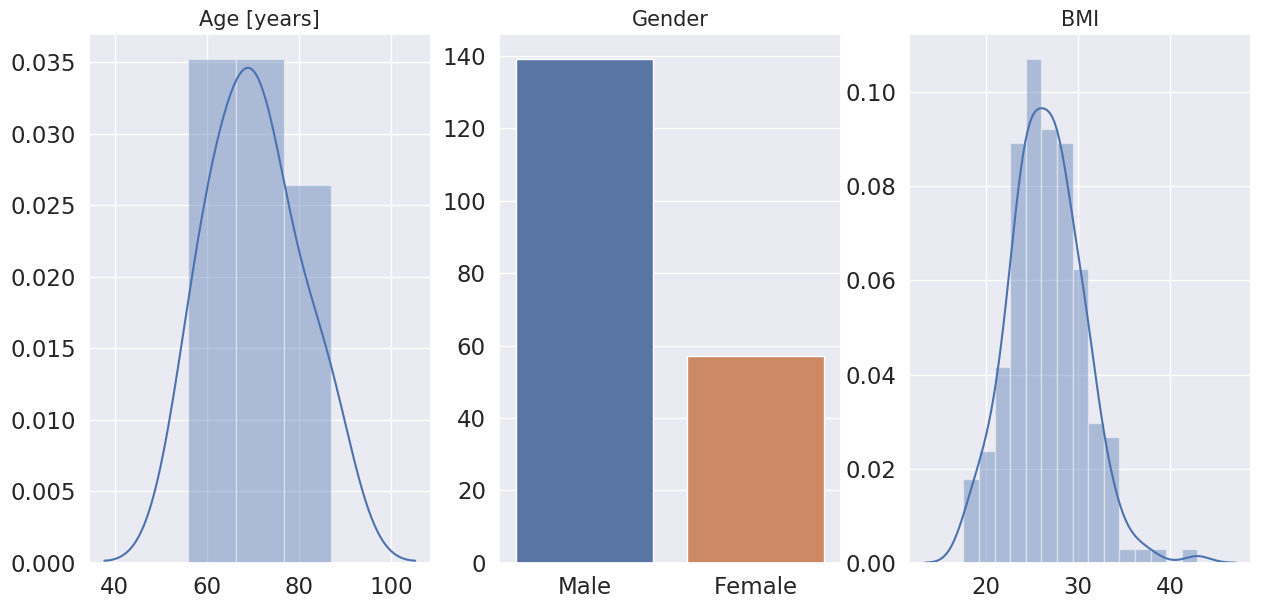
\includegraphics[width=\textwidth]{data-exp/metadataDist4.png}
    \end{center}
    \caption{Distribution of age, gender and BMI.}
    \label{fig:meta-dist4}
\end{figure}

\begin{figure}
    \begin{center}
    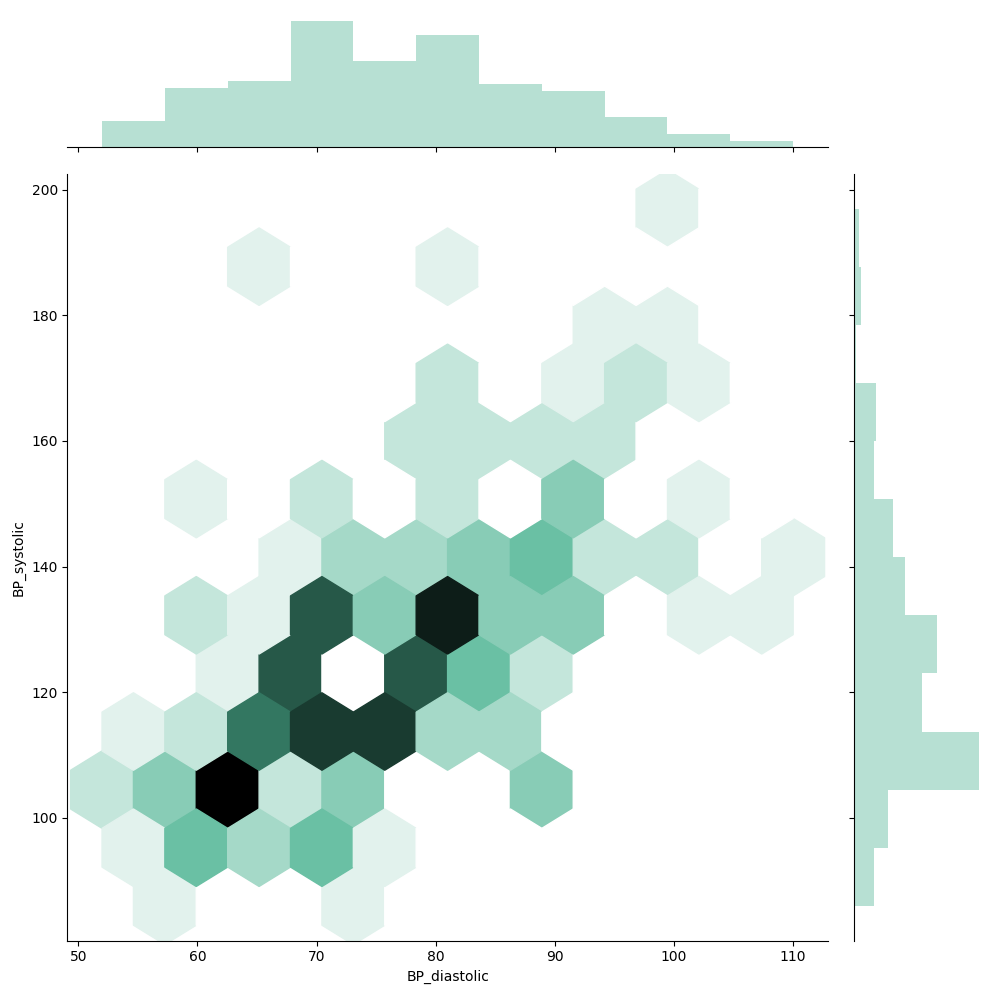
\includegraphics[width=0.4\textwidth]{data-exp/bp.png}
    \end{center}
    \caption{A joint distribtion plot of systolic and diastolic blood pressure of the patients.}
    \label{fig:bp-dist}
\end{figure}

Figure \ref{fig:meta-dist4} shows the patient distributions with regard to age, gender and BMI. As evident from the figure the patients that make up the dataset is made up of 138 males and 57 females. The majority of the patients are in the age group 60-80 years with a number of patients in the range 80-90 years (AGE SECTION SUBJECT TO CHANGE). The BMI distribution of patients is centered around 26 $kg/m^2$.Figure \ref{fig:bp-dist} shows the joint distribution of systolic and diastolic blood pressure among the patients.

\section{Input variables} \label{sec:covariates}
As mentioned earlier in section REF the different machine learning models that will be applied will apply two types of input data, time-series data in the form of longitudinal strain curves, and point-values in the form of peak systolic global longitudinal strain and patient EF.

\subsection{Peak-values}

\begin{figure}
    \begin{center}
    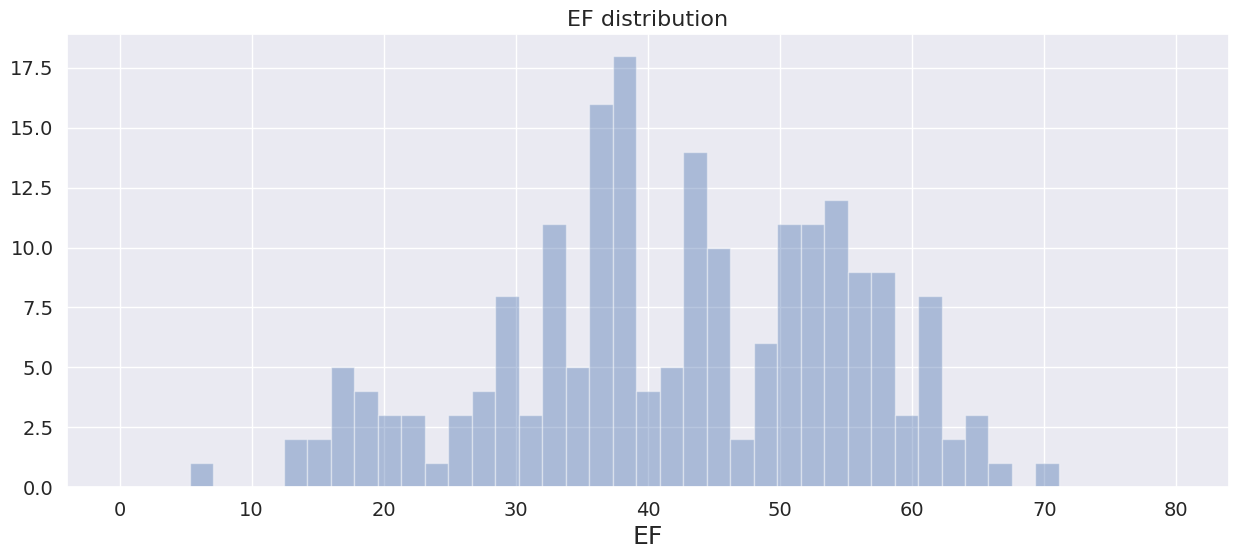
\includegraphics[width=0.4\textwidth]{data-exp/EF_dist.png}
    \end{center}
    \caption{Distribution of patient EF values.}
    \label{fig:}
\end{figure}

\begin{figure}
    \begin{center}
    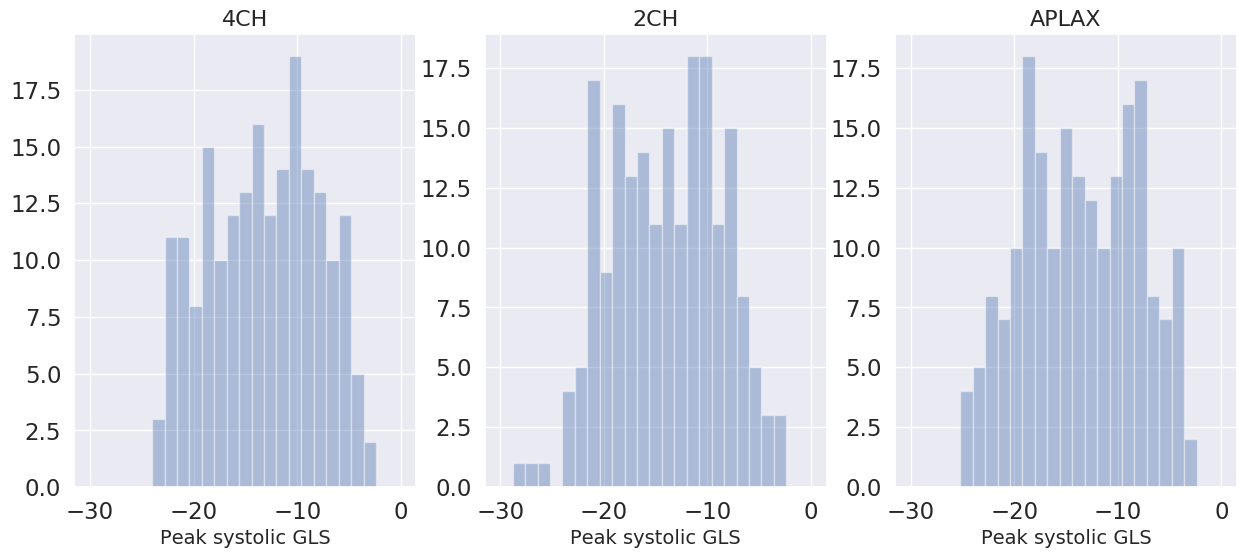
\includegraphics[width=0.4\textwidth]{data-exp/peak_sys_gls_dist.png}
    \end{center}
    \caption{Distribution of peak systolic global longitudinal strain.}
    \label{fig:}
\end{figure}

\subsection{Strain curves}

\begin{figure}
    \begin{center}
    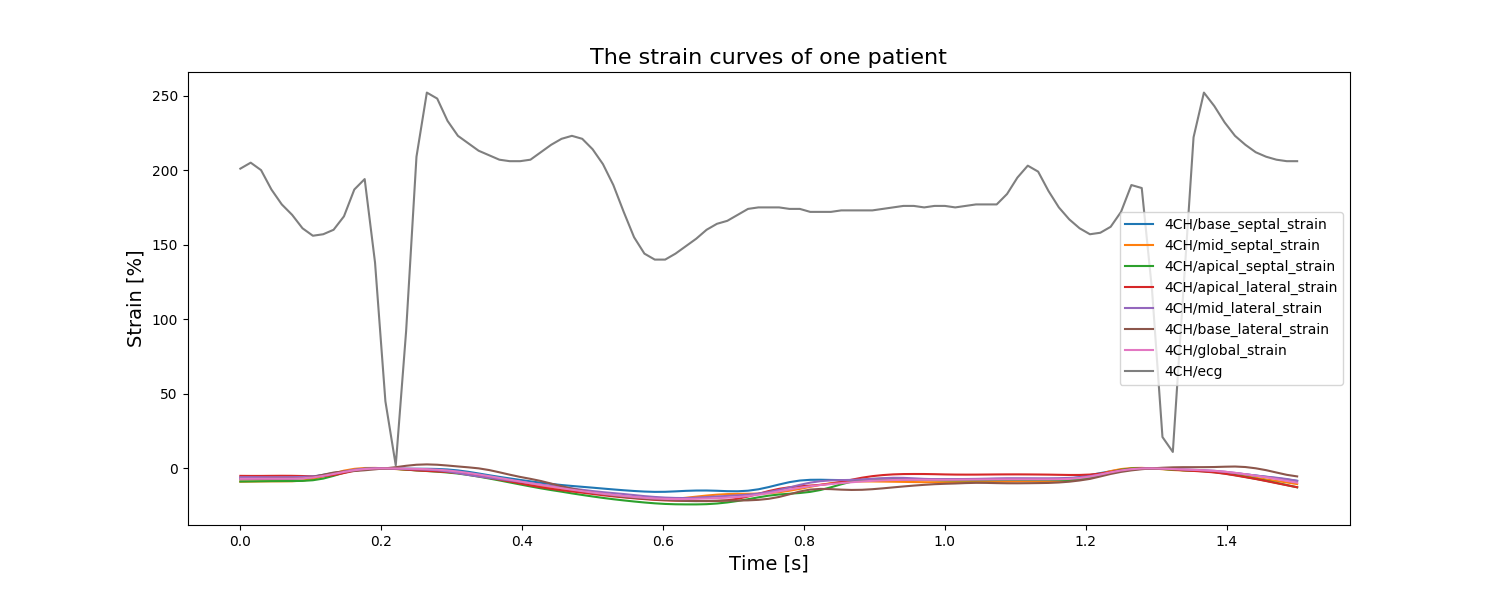
\includegraphics[width=0.4\textwidth]{data-exp/patient_strain_curves.png}
    \end{center}
    \caption{Plot of the global and regional longitudinal strain curves of one patient in the 4CH view.}
    \label{fig:}
\end{figure}

\section{Target variables} \label{sec:target}

\begin{figure}
    \begin{center}
    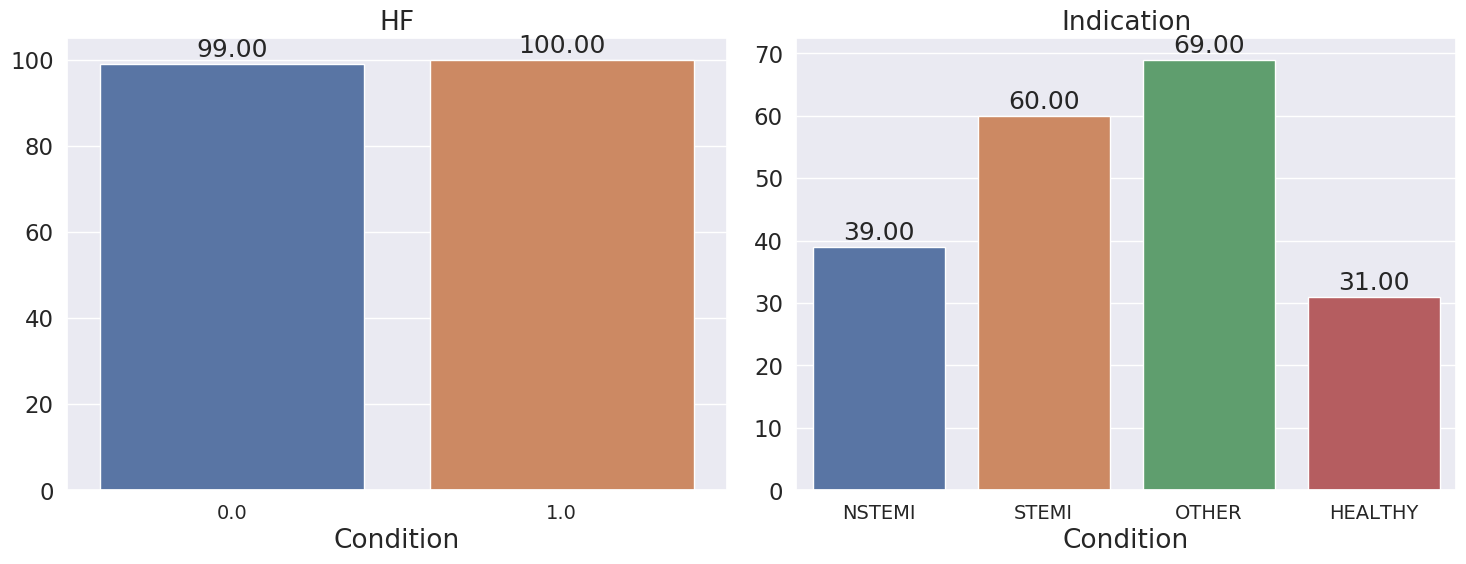
\includegraphics[width=0.4\textwidth]{data-exp/hf_indication_dist.png}
    \end{center}
    \caption{Distribution of heart failure within patients.}
    \label{fig:}
\end{figure}

\begin{figure}
    \begin{center}
    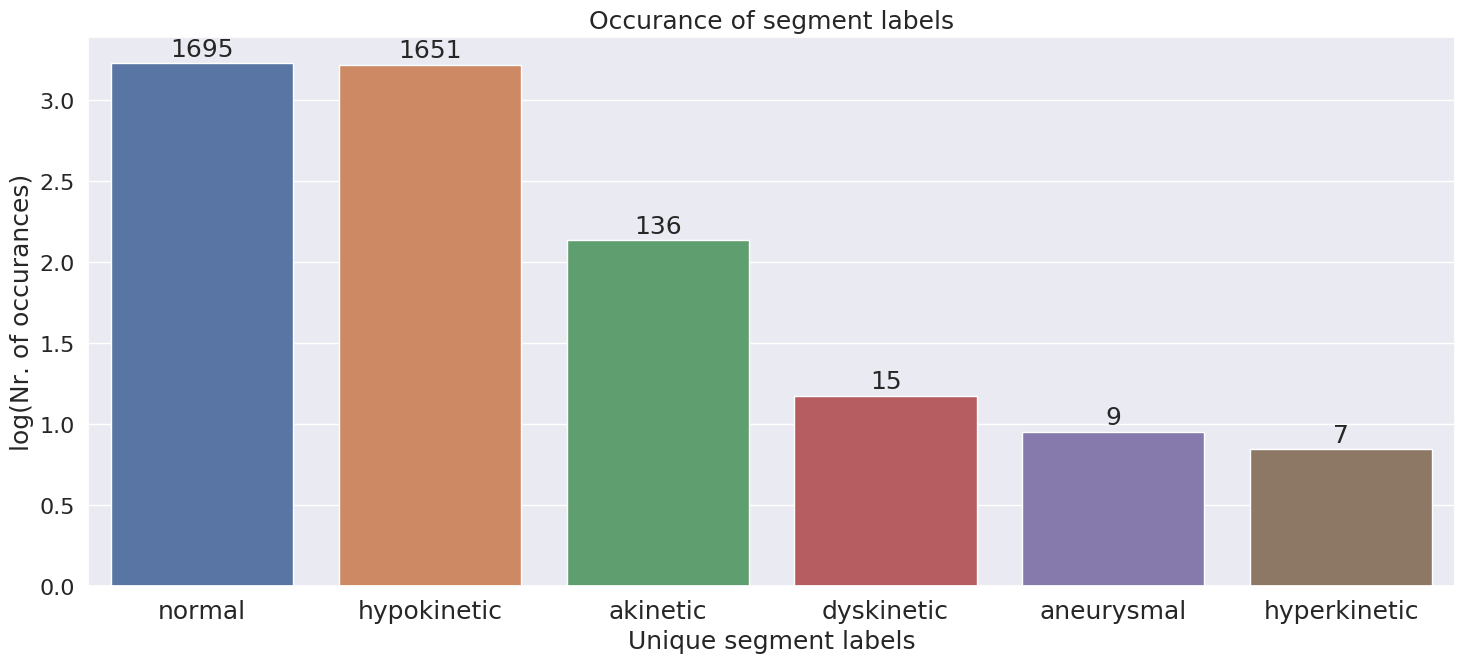
\includegraphics[width=0.4\textwidth]{data-exp/segment_label_distribution.png}
    \end{center}
    \caption{Distribution segment indication labels.}
    \label{fig:}
\end{figure}

\chapter{Method}

This is the section where we detail the specific models used. \bigskip

\section{Models} 

\subsection{Time-series clustering}

\subsection{Peak-value clustering}

\subsection{Recurrent Neural Network}

\subsection{Supervised Peak-value Classifiers}

\section{Description of The Datasets}

Since the different ML models detailed in chapter REFERENCE require different types of input data the, datasets have been divided into two main categories: 
The peak-value datasets and the time-series datasets. \bigskip

\subsection{Time-series Datasets}

\begin{table*}[h]
    \centering
    \ra{1.3}
    \begin{tabular}{ rlr }
        \toprule
        Nr & Input variables   & Shape \\
        \midrule
        1  & Single RLS curves & (3600, 1) \\
        2  & RLS curves        & (200, 18) \\
        3  & GLS curves        & (200, 3)  \\
        4  & Strain curves     & (200, 21) \\
        \bottomrule
    \end{tabular}
    \caption{Time-series datasets. The ''Shape'' parameter is indicates: (Number of objects in the dataset, Number of curves in each individual object). The curve length is not included in the shape parameter because it differs for different curves.}
    \label{tab:ts_dsets}
\end{table*}

Table \ref{tab:ts_dsets} shows the different time-series datasets that will be used. 
All the datasets except \textit{Single RLS curves} will be used to predict the diagnosis of patients, and whether the patient has heart failure.
Recall that the different diagnosises are described in section REFERENCE, and there occurance rate are illustrated in figure \ref{fig:hf_ind_dist}.
\textit{Single RLS curves} will be used to predict the segment indications shown in figure \ref{fig:segm_label_dis} and described in section REFERENCE. 
The point of classifying individual segments of a patients left ventricle is that if a single segment is found to be \textit{not normal}, 
this would also mean that the patient can be considered as \textit{not healthy}.
As mentioned in the description of table \ref{tab:ts_dsets} the ''Shape'' parameter shows how many objects each dataset has, and how many curves are associated to each object. 
Since each ultrasound examination takes ultrasound inspections from three views (four chamber, two chamber, and APLAX chamber), each patient has three views to estimate a GLS curve from. 
Since each GLS curve, also can be divided into six RLS curves, there is a total of 21 strain curves per patient. 
Since each patient has 18 RLS curves, there are $18 \times 200 = 3600$ curves that make up dataset number 1.
Both the RNN, and the TSC model are applied on the datasets listed in table \ref{tab:ts_dsets}, 
\bigskip

\textbf{NOT SURE ABOUT THIS ANYMORE}
however there have been made some significant changes to the multivariate time series to accomodate the DL model.
Even though RNNs are capable of handling objects of different sizes, the curves that make up a single object must be of the same size.
Since the strain curves extracted from different views often are of different lengths, the RNN has been limited to only using the strain curves associated with a single view
when evaluating the diagnosis, or heart failure status of one patient.

\subsection{Peak-value Datasets}

\begin{table*}[h]
    \centering
    \ra{1.3}
    \begin{tabular}{ rlr }
        \toprule
        Nr & Input variables                     & Shape \\
        \midrule                              
        1  & Single peak systolic RLS values     & (3600, 1) \\
        2  & Peak systolic RLS values            & (200, 18) \\
        3  & Peak systolic GLS values            & (200, 3)  \\
        4  & Peak systolic strain values         & (200, 21) \\
        5  & Peak systolic RLS, and EF values    & (200, 19) \\
        6  & Peak systolic GLS, and EF values    & (200, 4)  \\
        7  & Peak systolic strain, and EF values & (200, 22) \\
        \bottomrule
    \end{tabular}
    \caption{Peak-value datasets. The ''Shape'' parameter is indicates: (Number of objects in the dataset, Number of dimensions of each individual object).}
    \label{tab:pv_dsets}
\end{table*}

Table \ref{tab:pv_dsets} shows the different peak-value datasets. 
All the datasets with exception of \textit{Single peak systolic RLS values} will be used to predict the diagnosis of patients, and whether the patient has heart failure. 
\textit{Single peak systolic RLS values} is also the only peak-value dataset that is not suited for clustering, as a minimum of two dimensions is required to cluster a point-value dataset.
The reason that there are more peak-value datasets than there are time-series datasets, is that the peak-value version of three datasets in table \ref{tab:ts_dsets} have been combined 
with EF to determine whether a combination of peak systolic strain and EF can have a higher predictive power than strain alone.

\section{Case Studies}
The results of this paper will be presented in the form of three case studies. 
Each case study will focus on a single target variable, and aims to find which model group performs best at predicting the target variable in question.

Recall that the three target variables that will be considered in this thesis are: Heart failure, patient diagnosis, and the indication of individual left ventricle segments.
As mentioned previously in this chapter there are four main machine learning models that will be tested, but also many variations of these four models.
The variations within the main model categories differ slightly for the different subgroups. 
For the peak-value clustering models the variation between models is what dataset the model is applied on, what linkage is used to define the distance between cluster prototypes, and which number of clusters one chooses to divide the dataset into. 
For the time-series clustering models the variations are choice of dataset, which type of preprocessing is used, what linkage is used and the number of clusters.
For the RNN, the variations are choice of dataset and the type of preprocessing used. 
The main group of peak-value classifiers is a broad group which encompasses ten complex machine learning classifiers. 
No changes will be made to the hyperparameters of the individual models, so the variations in this group will be which particular classifier is used and which dataset the models are applied on. 
In each case study a brief discussion of performance of different model variations within each main category will be made, 
and then the best model variation will be used to compare the performance of the model groups.


\chapter{Results}

In this chapter the results will be presented in the form of three case studies. 
Each case study will focus on a single target variable, and aims to find which model group performs best at predicting the target variable in question.
Recall that the three target variables that will be considered in this thesis are: Heart failure, patient diagnosis, and the indication of individual left ventricle segments.
As mentioned earlier in the chapter, four model groups will be tested. 
The case studies will first deal with each model group individually, where variants of the models with different hypermarameters will be tested on the different datasets. 
Then, the best performing model within each model group will be used to compare the four model groups.

\section{Case Study: Heart Failure}

\subsection{Time-series Clustering}

\begin{figure}[htb]
    \centering
    % \includegraphics[width=\textwidth]{results/tsc_hf_dor_sens_spec_dist.png}
    %% Creator: Matplotlib, PGF backend
%%
%% To include the figure in your LaTeX document, write
%%   \input{<filename>.pgf}
%%
%% Make sure the required packages are loaded in your preamble
%%   \usepackage{pgf}
%%
%% Figures using additional raster images can only be included by \input if
%% they are in the same directory as the main LaTeX file. For loading figures
%% from other directories you can use the `import` package
%%   \usepackage{import}
%% and then include the figures with
%%   \import{<path to file>}{<filename>.pgf}
%%
%% Matplotlib used the following preamble
%%
\begingroup%
\makeatletter%
\begin{pgfpicture}%
\pgfpathrectangle{\pgfpointorigin}{\pgfqpoint{6.364000in}{2.340000in}}%
\pgfusepath{use as bounding box, clip}%
\begin{pgfscope}%
\pgfsetbuttcap%
\pgfsetmiterjoin%
\definecolor{currentfill}{rgb}{1.000000,1.000000,1.000000}%
\pgfsetfillcolor{currentfill}%
\pgfsetlinewidth{0.000000pt}%
\definecolor{currentstroke}{rgb}{1.000000,1.000000,1.000000}%
\pgfsetstrokecolor{currentstroke}%
\pgfsetdash{}{0pt}%
\pgfpathmoveto{\pgfqpoint{0.000000in}{-0.000000in}}%
\pgfpathlineto{\pgfqpoint{6.364000in}{-0.000000in}}%
\pgfpathlineto{\pgfqpoint{6.364000in}{2.340000in}}%
\pgfpathlineto{\pgfqpoint{0.000000in}{2.340000in}}%
\pgfpathclose%
\pgfusepath{fill}%
\end{pgfscope}%
\begin{pgfscope}%
\pgfsetbuttcap%
\pgfsetmiterjoin%
\definecolor{currentfill}{rgb}{0.917647,0.917647,0.949020}%
\pgfsetfillcolor{currentfill}%
\pgfsetlinewidth{0.000000pt}%
\definecolor{currentstroke}{rgb}{0.000000,0.000000,0.000000}%
\pgfsetstrokecolor{currentstroke}%
\pgfsetstrokeopacity{0.000000}%
\pgfsetdash{}{0pt}%
\pgfpathmoveto{\pgfqpoint{0.650810in}{0.557870in}}%
\pgfpathlineto{\pgfqpoint{3.096898in}{0.557870in}}%
\pgfpathlineto{\pgfqpoint{3.096898in}{2.042604in}}%
\pgfpathlineto{\pgfqpoint{0.650810in}{2.042604in}}%
\pgfpathclose%
\pgfusepath{fill}%
\end{pgfscope}%
\begin{pgfscope}%
\pgfpathrectangle{\pgfqpoint{0.650810in}{0.557870in}}{\pgfqpoint{2.446088in}{1.484734in}}%
\pgfusepath{clip}%
\pgfsetroundcap%
\pgfsetroundjoin%
\pgfsetlinewidth{1.003750pt}%
\definecolor{currentstroke}{rgb}{1.000000,1.000000,1.000000}%
\pgfsetstrokecolor{currentstroke}%
\pgfsetdash{}{0pt}%
\pgfpathmoveto{\pgfqpoint{0.761996in}{0.557870in}}%
\pgfpathlineto{\pgfqpoint{0.761996in}{2.042604in}}%
\pgfusepath{stroke}%
\end{pgfscope}%
\begin{pgfscope}%
\definecolor{textcolor}{rgb}{0.150000,0.150000,0.150000}%
\pgfsetstrokecolor{textcolor}%
\pgfsetfillcolor{textcolor}%
\pgftext[x=0.761996in,y=0.425926in,,top]{\color{textcolor}\sffamily\fontsize{11.000000}{13.200000}\selectfont \(\displaystyle -0.50\)}%
\end{pgfscope}%
\begin{pgfscope}%
\pgfpathrectangle{\pgfqpoint{0.650810in}{0.557870in}}{\pgfqpoint{2.446088in}{1.484734in}}%
\pgfusepath{clip}%
\pgfsetroundcap%
\pgfsetroundjoin%
\pgfsetlinewidth{1.003750pt}%
\definecolor{currentstroke}{rgb}{1.000000,1.000000,1.000000}%
\pgfsetstrokecolor{currentstroke}%
\pgfsetdash{}{0pt}%
\pgfpathmoveto{\pgfqpoint{1.317925in}{0.557870in}}%
\pgfpathlineto{\pgfqpoint{1.317925in}{2.042604in}}%
\pgfusepath{stroke}%
\end{pgfscope}%
\begin{pgfscope}%
\definecolor{textcolor}{rgb}{0.150000,0.150000,0.150000}%
\pgfsetstrokecolor{textcolor}%
\pgfsetfillcolor{textcolor}%
\pgftext[x=1.317925in,y=0.425926in,,top]{\color{textcolor}\sffamily\fontsize{11.000000}{13.200000}\selectfont \(\displaystyle -0.25\)}%
\end{pgfscope}%
\begin{pgfscope}%
\pgfpathrectangle{\pgfqpoint{0.650810in}{0.557870in}}{\pgfqpoint{2.446088in}{1.484734in}}%
\pgfusepath{clip}%
\pgfsetroundcap%
\pgfsetroundjoin%
\pgfsetlinewidth{1.003750pt}%
\definecolor{currentstroke}{rgb}{1.000000,1.000000,1.000000}%
\pgfsetstrokecolor{currentstroke}%
\pgfsetdash{}{0pt}%
\pgfpathmoveto{\pgfqpoint{1.873854in}{0.557870in}}%
\pgfpathlineto{\pgfqpoint{1.873854in}{2.042604in}}%
\pgfusepath{stroke}%
\end{pgfscope}%
\begin{pgfscope}%
\definecolor{textcolor}{rgb}{0.150000,0.150000,0.150000}%
\pgfsetstrokecolor{textcolor}%
\pgfsetfillcolor{textcolor}%
\pgftext[x=1.873854in,y=0.425926in,,top]{\color{textcolor}\sffamily\fontsize{11.000000}{13.200000}\selectfont \(\displaystyle 0.00\)}%
\end{pgfscope}%
\begin{pgfscope}%
\pgfpathrectangle{\pgfqpoint{0.650810in}{0.557870in}}{\pgfqpoint{2.446088in}{1.484734in}}%
\pgfusepath{clip}%
\pgfsetroundcap%
\pgfsetroundjoin%
\pgfsetlinewidth{1.003750pt}%
\definecolor{currentstroke}{rgb}{1.000000,1.000000,1.000000}%
\pgfsetstrokecolor{currentstroke}%
\pgfsetdash{}{0pt}%
\pgfpathmoveto{\pgfqpoint{2.429783in}{0.557870in}}%
\pgfpathlineto{\pgfqpoint{2.429783in}{2.042604in}}%
\pgfusepath{stroke}%
\end{pgfscope}%
\begin{pgfscope}%
\definecolor{textcolor}{rgb}{0.150000,0.150000,0.150000}%
\pgfsetstrokecolor{textcolor}%
\pgfsetfillcolor{textcolor}%
\pgftext[x=2.429783in,y=0.425926in,,top]{\color{textcolor}\sffamily\fontsize{11.000000}{13.200000}\selectfont \(\displaystyle 0.25\)}%
\end{pgfscope}%
\begin{pgfscope}%
\pgfpathrectangle{\pgfqpoint{0.650810in}{0.557870in}}{\pgfqpoint{2.446088in}{1.484734in}}%
\pgfusepath{clip}%
\pgfsetroundcap%
\pgfsetroundjoin%
\pgfsetlinewidth{1.003750pt}%
\definecolor{currentstroke}{rgb}{1.000000,1.000000,1.000000}%
\pgfsetstrokecolor{currentstroke}%
\pgfsetdash{}{0pt}%
\pgfpathmoveto{\pgfqpoint{2.985712in}{0.557870in}}%
\pgfpathlineto{\pgfqpoint{2.985712in}{2.042604in}}%
\pgfusepath{stroke}%
\end{pgfscope}%
\begin{pgfscope}%
\definecolor{textcolor}{rgb}{0.150000,0.150000,0.150000}%
\pgfsetstrokecolor{textcolor}%
\pgfsetfillcolor{textcolor}%
\pgftext[x=2.985712in,y=0.425926in,,top]{\color{textcolor}\sffamily\fontsize{11.000000}{13.200000}\selectfont \(\displaystyle 0.50\)}%
\end{pgfscope}%
\begin{pgfscope}%
\definecolor{textcolor}{rgb}{0.150000,0.150000,0.150000}%
\pgfsetstrokecolor{textcolor}%
\pgfsetfillcolor{textcolor}%
\pgftext[x=1.873854in,y=0.235185in,,top]{\color{textcolor}\sffamily\fontsize{11.000000}{13.200000}\selectfont DOR}%
\end{pgfscope}%
\begin{pgfscope}%
\pgfpathrectangle{\pgfqpoint{0.650810in}{0.557870in}}{\pgfqpoint{2.446088in}{1.484734in}}%
\pgfusepath{clip}%
\pgfsetroundcap%
\pgfsetroundjoin%
\pgfsetlinewidth{1.003750pt}%
\definecolor{currentstroke}{rgb}{1.000000,1.000000,1.000000}%
\pgfsetstrokecolor{currentstroke}%
\pgfsetdash{}{0pt}%
\pgfpathmoveto{\pgfqpoint{0.650810in}{0.557870in}}%
\pgfpathlineto{\pgfqpoint{3.096898in}{0.557870in}}%
\pgfusepath{stroke}%
\end{pgfscope}%
\begin{pgfscope}%
\definecolor{textcolor}{rgb}{0.150000,0.150000,0.150000}%
\pgfsetstrokecolor{textcolor}%
\pgfsetfillcolor{textcolor}%
\pgftext[x=0.442824in,y=0.505064in,left,base]{\color{textcolor}\sffamily\fontsize{11.000000}{13.200000}\selectfont \(\displaystyle 0\)}%
\end{pgfscope}%
\begin{pgfscope}%
\pgfpathrectangle{\pgfqpoint{0.650810in}{0.557870in}}{\pgfqpoint{2.446088in}{1.484734in}}%
\pgfusepath{clip}%
\pgfsetroundcap%
\pgfsetroundjoin%
\pgfsetlinewidth{1.003750pt}%
\definecolor{currentstroke}{rgb}{1.000000,1.000000,1.000000}%
\pgfsetstrokecolor{currentstroke}%
\pgfsetdash{}{0pt}%
\pgfpathmoveto{\pgfqpoint{0.650810in}{1.032378in}}%
\pgfpathlineto{\pgfqpoint{3.096898in}{1.032378in}}%
\pgfusepath{stroke}%
\end{pgfscope}%
\begin{pgfscope}%
\definecolor{textcolor}{rgb}{0.150000,0.150000,0.150000}%
\pgfsetstrokecolor{textcolor}%
\pgfsetfillcolor{textcolor}%
\pgftext[x=0.290741in,y=0.979571in,left,base]{\color{textcolor}\sffamily\fontsize{11.000000}{13.200000}\selectfont \(\displaystyle 100\)}%
\end{pgfscope}%
\begin{pgfscope}%
\pgfpathrectangle{\pgfqpoint{0.650810in}{0.557870in}}{\pgfqpoint{2.446088in}{1.484734in}}%
\pgfusepath{clip}%
\pgfsetroundcap%
\pgfsetroundjoin%
\pgfsetlinewidth{1.003750pt}%
\definecolor{currentstroke}{rgb}{1.000000,1.000000,1.000000}%
\pgfsetstrokecolor{currentstroke}%
\pgfsetdash{}{0pt}%
\pgfpathmoveto{\pgfqpoint{0.650810in}{1.506885in}}%
\pgfpathlineto{\pgfqpoint{3.096898in}{1.506885in}}%
\pgfusepath{stroke}%
\end{pgfscope}%
\begin{pgfscope}%
\definecolor{textcolor}{rgb}{0.150000,0.150000,0.150000}%
\pgfsetstrokecolor{textcolor}%
\pgfsetfillcolor{textcolor}%
\pgftext[x=0.290741in,y=1.454079in,left,base]{\color{textcolor}\sffamily\fontsize{11.000000}{13.200000}\selectfont \(\displaystyle 200\)}%
\end{pgfscope}%
\begin{pgfscope}%
\pgfpathrectangle{\pgfqpoint{0.650810in}{0.557870in}}{\pgfqpoint{2.446088in}{1.484734in}}%
\pgfusepath{clip}%
\pgfsetroundcap%
\pgfsetroundjoin%
\pgfsetlinewidth{1.003750pt}%
\definecolor{currentstroke}{rgb}{1.000000,1.000000,1.000000}%
\pgfsetstrokecolor{currentstroke}%
\pgfsetdash{}{0pt}%
\pgfpathmoveto{\pgfqpoint{0.650810in}{1.981393in}}%
\pgfpathlineto{\pgfqpoint{3.096898in}{1.981393in}}%
\pgfusepath{stroke}%
\end{pgfscope}%
\begin{pgfscope}%
\definecolor{textcolor}{rgb}{0.150000,0.150000,0.150000}%
\pgfsetstrokecolor{textcolor}%
\pgfsetfillcolor{textcolor}%
\pgftext[x=0.290741in,y=1.928586in,left,base]{\color{textcolor}\sffamily\fontsize{11.000000}{13.200000}\selectfont \(\displaystyle 300\)}%
\end{pgfscope}%
\begin{pgfscope}%
\definecolor{textcolor}{rgb}{0.150000,0.150000,0.150000}%
\pgfsetstrokecolor{textcolor}%
\pgfsetfillcolor{textcolor}%
\pgftext[x=0.235185in,y=1.300237in,,bottom,rotate=90.000000]{\color{textcolor}\sffamily\fontsize{11.000000}{13.200000}\selectfont Occurance}%
\end{pgfscope}%
\begin{pgfscope}%
\pgfpathrectangle{\pgfqpoint{0.650810in}{0.557870in}}{\pgfqpoint{2.446088in}{1.484734in}}%
\pgfusepath{clip}%
\pgfsetbuttcap%
\pgfsetmiterjoin%
\definecolor{currentfill}{rgb}{0.298039,0.447059,0.690196}%
\pgfsetfillcolor{currentfill}%
\pgfsetfillopacity{0.400000}%
\pgfsetlinewidth{1.003750pt}%
\definecolor{currentstroke}{rgb}{1.000000,1.000000,1.000000}%
\pgfsetstrokecolor{currentstroke}%
\pgfsetstrokeopacity{0.400000}%
\pgfsetdash{}{0pt}%
\pgfpathmoveto{\pgfqpoint{0.761996in}{0.557870in}}%
\pgfpathlineto{\pgfqpoint{0.984368in}{0.557870in}}%
\pgfpathlineto{\pgfqpoint{0.984368in}{0.557870in}}%
\pgfpathlineto{\pgfqpoint{0.761996in}{0.557870in}}%
\pgfpathclose%
\pgfusepath{stroke,fill}%
\end{pgfscope}%
\begin{pgfscope}%
\pgfpathrectangle{\pgfqpoint{0.650810in}{0.557870in}}{\pgfqpoint{2.446088in}{1.484734in}}%
\pgfusepath{clip}%
\pgfsetbuttcap%
\pgfsetmiterjoin%
\definecolor{currentfill}{rgb}{0.298039,0.447059,0.690196}%
\pgfsetfillcolor{currentfill}%
\pgfsetfillopacity{0.400000}%
\pgfsetlinewidth{1.003750pt}%
\definecolor{currentstroke}{rgb}{1.000000,1.000000,1.000000}%
\pgfsetstrokecolor{currentstroke}%
\pgfsetstrokeopacity{0.400000}%
\pgfsetdash{}{0pt}%
\pgfpathmoveto{\pgfqpoint{0.984368in}{0.557870in}}%
\pgfpathlineto{\pgfqpoint{1.206739in}{0.557870in}}%
\pgfpathlineto{\pgfqpoint{1.206739in}{0.557870in}}%
\pgfpathlineto{\pgfqpoint{0.984368in}{0.557870in}}%
\pgfpathclose%
\pgfusepath{stroke,fill}%
\end{pgfscope}%
\begin{pgfscope}%
\pgfpathrectangle{\pgfqpoint{0.650810in}{0.557870in}}{\pgfqpoint{2.446088in}{1.484734in}}%
\pgfusepath{clip}%
\pgfsetbuttcap%
\pgfsetmiterjoin%
\definecolor{currentfill}{rgb}{0.298039,0.447059,0.690196}%
\pgfsetfillcolor{currentfill}%
\pgfsetfillopacity{0.400000}%
\pgfsetlinewidth{1.003750pt}%
\definecolor{currentstroke}{rgb}{1.000000,1.000000,1.000000}%
\pgfsetstrokecolor{currentstroke}%
\pgfsetstrokeopacity{0.400000}%
\pgfsetdash{}{0pt}%
\pgfpathmoveto{\pgfqpoint{1.206739in}{0.557870in}}%
\pgfpathlineto{\pgfqpoint{1.429111in}{0.557870in}}%
\pgfpathlineto{\pgfqpoint{1.429111in}{0.557870in}}%
\pgfpathlineto{\pgfqpoint{1.206739in}{0.557870in}}%
\pgfpathclose%
\pgfusepath{stroke,fill}%
\end{pgfscope}%
\begin{pgfscope}%
\pgfpathrectangle{\pgfqpoint{0.650810in}{0.557870in}}{\pgfqpoint{2.446088in}{1.484734in}}%
\pgfusepath{clip}%
\pgfsetbuttcap%
\pgfsetmiterjoin%
\definecolor{currentfill}{rgb}{0.298039,0.447059,0.690196}%
\pgfsetfillcolor{currentfill}%
\pgfsetfillopacity{0.400000}%
\pgfsetlinewidth{1.003750pt}%
\definecolor{currentstroke}{rgb}{1.000000,1.000000,1.000000}%
\pgfsetstrokecolor{currentstroke}%
\pgfsetstrokeopacity{0.400000}%
\pgfsetdash{}{0pt}%
\pgfpathmoveto{\pgfqpoint{1.429111in}{0.557870in}}%
\pgfpathlineto{\pgfqpoint{1.651483in}{0.557870in}}%
\pgfpathlineto{\pgfqpoint{1.651483in}{0.557870in}}%
\pgfpathlineto{\pgfqpoint{1.429111in}{0.557870in}}%
\pgfpathclose%
\pgfusepath{stroke,fill}%
\end{pgfscope}%
\begin{pgfscope}%
\pgfpathrectangle{\pgfqpoint{0.650810in}{0.557870in}}{\pgfqpoint{2.446088in}{1.484734in}}%
\pgfusepath{clip}%
\pgfsetbuttcap%
\pgfsetmiterjoin%
\definecolor{currentfill}{rgb}{0.298039,0.447059,0.690196}%
\pgfsetfillcolor{currentfill}%
\pgfsetfillopacity{0.400000}%
\pgfsetlinewidth{1.003750pt}%
\definecolor{currentstroke}{rgb}{1.000000,1.000000,1.000000}%
\pgfsetstrokecolor{currentstroke}%
\pgfsetstrokeopacity{0.400000}%
\pgfsetdash{}{0pt}%
\pgfpathmoveto{\pgfqpoint{1.651483in}{0.557870in}}%
\pgfpathlineto{\pgfqpoint{1.873854in}{0.557870in}}%
\pgfpathlineto{\pgfqpoint{1.873854in}{0.557870in}}%
\pgfpathlineto{\pgfqpoint{1.651483in}{0.557870in}}%
\pgfpathclose%
\pgfusepath{stroke,fill}%
\end{pgfscope}%
\begin{pgfscope}%
\pgfpathrectangle{\pgfqpoint{0.650810in}{0.557870in}}{\pgfqpoint{2.446088in}{1.484734in}}%
\pgfusepath{clip}%
\pgfsetbuttcap%
\pgfsetmiterjoin%
\definecolor{currentfill}{rgb}{0.298039,0.447059,0.690196}%
\pgfsetfillcolor{currentfill}%
\pgfsetfillopacity{0.400000}%
\pgfsetlinewidth{1.003750pt}%
\definecolor{currentstroke}{rgb}{1.000000,1.000000,1.000000}%
\pgfsetstrokecolor{currentstroke}%
\pgfsetstrokeopacity{0.400000}%
\pgfsetdash{}{0pt}%
\pgfpathmoveto{\pgfqpoint{1.873854in}{0.557870in}}%
\pgfpathlineto{\pgfqpoint{2.096226in}{0.557870in}}%
\pgfpathlineto{\pgfqpoint{2.096226in}{1.971903in}}%
\pgfpathlineto{\pgfqpoint{1.873854in}{1.971903in}}%
\pgfpathclose%
\pgfusepath{stroke,fill}%
\end{pgfscope}%
\begin{pgfscope}%
\pgfpathrectangle{\pgfqpoint{0.650810in}{0.557870in}}{\pgfqpoint{2.446088in}{1.484734in}}%
\pgfusepath{clip}%
\pgfsetbuttcap%
\pgfsetmiterjoin%
\definecolor{currentfill}{rgb}{0.298039,0.447059,0.690196}%
\pgfsetfillcolor{currentfill}%
\pgfsetfillopacity{0.400000}%
\pgfsetlinewidth{1.003750pt}%
\definecolor{currentstroke}{rgb}{1.000000,1.000000,1.000000}%
\pgfsetstrokecolor{currentstroke}%
\pgfsetstrokeopacity{0.400000}%
\pgfsetdash{}{0pt}%
\pgfpathmoveto{\pgfqpoint{2.096226in}{0.557870in}}%
\pgfpathlineto{\pgfqpoint{2.318598in}{0.557870in}}%
\pgfpathlineto{\pgfqpoint{2.318598in}{0.557870in}}%
\pgfpathlineto{\pgfqpoint{2.096226in}{0.557870in}}%
\pgfpathclose%
\pgfusepath{stroke,fill}%
\end{pgfscope}%
\begin{pgfscope}%
\pgfpathrectangle{\pgfqpoint{0.650810in}{0.557870in}}{\pgfqpoint{2.446088in}{1.484734in}}%
\pgfusepath{clip}%
\pgfsetbuttcap%
\pgfsetmiterjoin%
\definecolor{currentfill}{rgb}{0.298039,0.447059,0.690196}%
\pgfsetfillcolor{currentfill}%
\pgfsetfillopacity{0.400000}%
\pgfsetlinewidth{1.003750pt}%
\definecolor{currentstroke}{rgb}{1.000000,1.000000,1.000000}%
\pgfsetstrokecolor{currentstroke}%
\pgfsetstrokeopacity{0.400000}%
\pgfsetdash{}{0pt}%
\pgfpathmoveto{\pgfqpoint{2.318598in}{0.557870in}}%
\pgfpathlineto{\pgfqpoint{2.540969in}{0.557870in}}%
\pgfpathlineto{\pgfqpoint{2.540969in}{0.557870in}}%
\pgfpathlineto{\pgfqpoint{2.318598in}{0.557870in}}%
\pgfpathclose%
\pgfusepath{stroke,fill}%
\end{pgfscope}%
\begin{pgfscope}%
\pgfpathrectangle{\pgfqpoint{0.650810in}{0.557870in}}{\pgfqpoint{2.446088in}{1.484734in}}%
\pgfusepath{clip}%
\pgfsetbuttcap%
\pgfsetmiterjoin%
\definecolor{currentfill}{rgb}{0.298039,0.447059,0.690196}%
\pgfsetfillcolor{currentfill}%
\pgfsetfillopacity{0.400000}%
\pgfsetlinewidth{1.003750pt}%
\definecolor{currentstroke}{rgb}{1.000000,1.000000,1.000000}%
\pgfsetstrokecolor{currentstroke}%
\pgfsetstrokeopacity{0.400000}%
\pgfsetdash{}{0pt}%
\pgfpathmoveto{\pgfqpoint{2.540969in}{0.557870in}}%
\pgfpathlineto{\pgfqpoint{2.763341in}{0.557870in}}%
\pgfpathlineto{\pgfqpoint{2.763341in}{0.557870in}}%
\pgfpathlineto{\pgfqpoint{2.540969in}{0.557870in}}%
\pgfpathclose%
\pgfusepath{stroke,fill}%
\end{pgfscope}%
\begin{pgfscope}%
\pgfpathrectangle{\pgfqpoint{0.650810in}{0.557870in}}{\pgfqpoint{2.446088in}{1.484734in}}%
\pgfusepath{clip}%
\pgfsetbuttcap%
\pgfsetmiterjoin%
\definecolor{currentfill}{rgb}{0.298039,0.447059,0.690196}%
\pgfsetfillcolor{currentfill}%
\pgfsetfillopacity{0.400000}%
\pgfsetlinewidth{1.003750pt}%
\definecolor{currentstroke}{rgb}{1.000000,1.000000,1.000000}%
\pgfsetstrokecolor{currentstroke}%
\pgfsetstrokeopacity{0.400000}%
\pgfsetdash{}{0pt}%
\pgfpathmoveto{\pgfqpoint{2.763341in}{0.557870in}}%
\pgfpathlineto{\pgfqpoint{2.985712in}{0.557870in}}%
\pgfpathlineto{\pgfqpoint{2.985712in}{0.557870in}}%
\pgfpathlineto{\pgfqpoint{2.763341in}{0.557870in}}%
\pgfpathclose%
\pgfusepath{stroke,fill}%
\end{pgfscope}%
\begin{pgfscope}%
\pgfsetrectcap%
\pgfsetmiterjoin%
\pgfsetlinewidth{1.254687pt}%
\definecolor{currentstroke}{rgb}{1.000000,1.000000,1.000000}%
\pgfsetstrokecolor{currentstroke}%
\pgfsetdash{}{0pt}%
\pgfpathmoveto{\pgfqpoint{0.650810in}{0.557870in}}%
\pgfpathlineto{\pgfqpoint{0.650810in}{2.042604in}}%
\pgfusepath{stroke}%
\end{pgfscope}%
\begin{pgfscope}%
\pgfsetrectcap%
\pgfsetmiterjoin%
\pgfsetlinewidth{1.254687pt}%
\definecolor{currentstroke}{rgb}{1.000000,1.000000,1.000000}%
\pgfsetstrokecolor{currentstroke}%
\pgfsetdash{}{0pt}%
\pgfpathmoveto{\pgfqpoint{3.096898in}{0.557870in}}%
\pgfpathlineto{\pgfqpoint{3.096898in}{2.042604in}}%
\pgfusepath{stroke}%
\end{pgfscope}%
\begin{pgfscope}%
\pgfsetrectcap%
\pgfsetmiterjoin%
\pgfsetlinewidth{1.254687pt}%
\definecolor{currentstroke}{rgb}{1.000000,1.000000,1.000000}%
\pgfsetstrokecolor{currentstroke}%
\pgfsetdash{}{0pt}%
\pgfpathmoveto{\pgfqpoint{0.650810in}{0.557870in}}%
\pgfpathlineto{\pgfqpoint{3.096898in}{0.557870in}}%
\pgfusepath{stroke}%
\end{pgfscope}%
\begin{pgfscope}%
\pgfsetrectcap%
\pgfsetmiterjoin%
\pgfsetlinewidth{1.254687pt}%
\definecolor{currentstroke}{rgb}{1.000000,1.000000,1.000000}%
\pgfsetstrokecolor{currentstroke}%
\pgfsetdash{}{0pt}%
\pgfpathmoveto{\pgfqpoint{0.650810in}{2.042604in}}%
\pgfpathlineto{\pgfqpoint{3.096898in}{2.042604in}}%
\pgfusepath{stroke}%
\end{pgfscope}%
\begin{pgfscope}%
\definecolor{textcolor}{rgb}{0.150000,0.150000,0.150000}%
\pgfsetstrokecolor{textcolor}%
\pgfsetfillcolor{textcolor}%
\pgftext[x=1.873854in,y=2.125938in,,base]{\color{textcolor}\sffamily\fontsize{11.000000}{13.200000}\selectfont (a)}%
\end{pgfscope}%
\begin{pgfscope}%
\pgfsetbuttcap%
\pgfsetmiterjoin%
\definecolor{currentfill}{rgb}{0.917647,0.917647,0.949020}%
\pgfsetfillcolor{currentfill}%
\pgfsetlinewidth{0.000000pt}%
\definecolor{currentstroke}{rgb}{0.000000,0.000000,0.000000}%
\pgfsetstrokecolor{currentstroke}%
\pgfsetstrokeopacity{0.000000}%
\pgfsetdash{}{0pt}%
\pgfpathmoveto{\pgfqpoint{3.793912in}{0.557870in}}%
\pgfpathlineto{\pgfqpoint{6.240000in}{0.557870in}}%
\pgfpathlineto{\pgfqpoint{6.240000in}{2.042604in}}%
\pgfpathlineto{\pgfqpoint{3.793912in}{2.042604in}}%
\pgfpathclose%
\pgfusepath{fill}%
\end{pgfscope}%
\begin{pgfscope}%
\pgfpathrectangle{\pgfqpoint{3.793912in}{0.557870in}}{\pgfqpoint{2.446088in}{1.484734in}}%
\pgfusepath{clip}%
\pgfsetroundcap%
\pgfsetroundjoin%
\pgfsetlinewidth{1.003750pt}%
\definecolor{currentstroke}{rgb}{1.000000,1.000000,1.000000}%
\pgfsetstrokecolor{currentstroke}%
\pgfsetdash{}{0pt}%
\pgfpathmoveto{\pgfqpoint{3.905098in}{0.557870in}}%
\pgfpathlineto{\pgfqpoint{3.905098in}{2.042604in}}%
\pgfusepath{stroke}%
\end{pgfscope}%
\begin{pgfscope}%
\definecolor{textcolor}{rgb}{0.150000,0.150000,0.150000}%
\pgfsetstrokecolor{textcolor}%
\pgfsetfillcolor{textcolor}%
\pgftext[x=3.905098in,y=0.425926in,,top]{\color{textcolor}\sffamily\fontsize{11.000000}{13.200000}\selectfont \(\displaystyle 0.00\)}%
\end{pgfscope}%
\begin{pgfscope}%
\pgfpathrectangle{\pgfqpoint{3.793912in}{0.557870in}}{\pgfqpoint{2.446088in}{1.484734in}}%
\pgfusepath{clip}%
\pgfsetroundcap%
\pgfsetroundjoin%
\pgfsetlinewidth{1.003750pt}%
\definecolor{currentstroke}{rgb}{1.000000,1.000000,1.000000}%
\pgfsetstrokecolor{currentstroke}%
\pgfsetdash{}{0pt}%
\pgfpathmoveto{\pgfqpoint{4.461027in}{0.557870in}}%
\pgfpathlineto{\pgfqpoint{4.461027in}{2.042604in}}%
\pgfusepath{stroke}%
\end{pgfscope}%
\begin{pgfscope}%
\definecolor{textcolor}{rgb}{0.150000,0.150000,0.150000}%
\pgfsetstrokecolor{textcolor}%
\pgfsetfillcolor{textcolor}%
\pgftext[x=4.461027in,y=0.425926in,,top]{\color{textcolor}\sffamily\fontsize{11.000000}{13.200000}\selectfont \(\displaystyle 0.25\)}%
\end{pgfscope}%
\begin{pgfscope}%
\pgfpathrectangle{\pgfqpoint{3.793912in}{0.557870in}}{\pgfqpoint{2.446088in}{1.484734in}}%
\pgfusepath{clip}%
\pgfsetroundcap%
\pgfsetroundjoin%
\pgfsetlinewidth{1.003750pt}%
\definecolor{currentstroke}{rgb}{1.000000,1.000000,1.000000}%
\pgfsetstrokecolor{currentstroke}%
\pgfsetdash{}{0pt}%
\pgfpathmoveto{\pgfqpoint{5.016956in}{0.557870in}}%
\pgfpathlineto{\pgfqpoint{5.016956in}{2.042604in}}%
\pgfusepath{stroke}%
\end{pgfscope}%
\begin{pgfscope}%
\definecolor{textcolor}{rgb}{0.150000,0.150000,0.150000}%
\pgfsetstrokecolor{textcolor}%
\pgfsetfillcolor{textcolor}%
\pgftext[x=5.016956in,y=0.425926in,,top]{\color{textcolor}\sffamily\fontsize{11.000000}{13.200000}\selectfont \(\displaystyle 0.50\)}%
\end{pgfscope}%
\begin{pgfscope}%
\pgfpathrectangle{\pgfqpoint{3.793912in}{0.557870in}}{\pgfqpoint{2.446088in}{1.484734in}}%
\pgfusepath{clip}%
\pgfsetroundcap%
\pgfsetroundjoin%
\pgfsetlinewidth{1.003750pt}%
\definecolor{currentstroke}{rgb}{1.000000,1.000000,1.000000}%
\pgfsetstrokecolor{currentstroke}%
\pgfsetdash{}{0pt}%
\pgfpathmoveto{\pgfqpoint{5.572885in}{0.557870in}}%
\pgfpathlineto{\pgfqpoint{5.572885in}{2.042604in}}%
\pgfusepath{stroke}%
\end{pgfscope}%
\begin{pgfscope}%
\definecolor{textcolor}{rgb}{0.150000,0.150000,0.150000}%
\pgfsetstrokecolor{textcolor}%
\pgfsetfillcolor{textcolor}%
\pgftext[x=5.572885in,y=0.425926in,,top]{\color{textcolor}\sffamily\fontsize{11.000000}{13.200000}\selectfont \(\displaystyle 0.75\)}%
\end{pgfscope}%
\begin{pgfscope}%
\pgfpathrectangle{\pgfqpoint{3.793912in}{0.557870in}}{\pgfqpoint{2.446088in}{1.484734in}}%
\pgfusepath{clip}%
\pgfsetroundcap%
\pgfsetroundjoin%
\pgfsetlinewidth{1.003750pt}%
\definecolor{currentstroke}{rgb}{1.000000,1.000000,1.000000}%
\pgfsetstrokecolor{currentstroke}%
\pgfsetdash{}{0pt}%
\pgfpathmoveto{\pgfqpoint{6.128814in}{0.557870in}}%
\pgfpathlineto{\pgfqpoint{6.128814in}{2.042604in}}%
\pgfusepath{stroke}%
\end{pgfscope}%
\begin{pgfscope}%
\definecolor{textcolor}{rgb}{0.150000,0.150000,0.150000}%
\pgfsetstrokecolor{textcolor}%
\pgfsetfillcolor{textcolor}%
\pgftext[x=6.128814in,y=0.425926in,,top]{\color{textcolor}\sffamily\fontsize{11.000000}{13.200000}\selectfont \(\displaystyle 1.00\)}%
\end{pgfscope}%
\begin{pgfscope}%
\definecolor{textcolor}{rgb}{0.150000,0.150000,0.150000}%
\pgfsetstrokecolor{textcolor}%
\pgfsetfillcolor{textcolor}%
\pgftext[x=5.016956in,y=0.235185in,,top]{\color{textcolor}\sffamily\fontsize{11.000000}{13.200000}\selectfont Specificity}%
\end{pgfscope}%
\begin{pgfscope}%
\pgfpathrectangle{\pgfqpoint{3.793912in}{0.557870in}}{\pgfqpoint{2.446088in}{1.484734in}}%
\pgfusepath{clip}%
\pgfsetroundcap%
\pgfsetroundjoin%
\pgfsetlinewidth{1.003750pt}%
\definecolor{currentstroke}{rgb}{1.000000,1.000000,1.000000}%
\pgfsetstrokecolor{currentstroke}%
\pgfsetdash{}{0pt}%
\pgfpathmoveto{\pgfqpoint{3.793912in}{0.625358in}}%
\pgfpathlineto{\pgfqpoint{6.240000in}{0.625358in}}%
\pgfusepath{stroke}%
\end{pgfscope}%
\begin{pgfscope}%
\definecolor{textcolor}{rgb}{0.150000,0.150000,0.150000}%
\pgfsetstrokecolor{textcolor}%
\pgfsetfillcolor{textcolor}%
\pgftext[x=3.467639in,y=0.572552in,left,base]{\color{textcolor}\sffamily\fontsize{11.000000}{13.200000}\selectfont \(\displaystyle 0.0\)}%
\end{pgfscope}%
\begin{pgfscope}%
\pgfpathrectangle{\pgfqpoint{3.793912in}{0.557870in}}{\pgfqpoint{2.446088in}{1.484734in}}%
\pgfusepath{clip}%
\pgfsetroundcap%
\pgfsetroundjoin%
\pgfsetlinewidth{1.003750pt}%
\definecolor{currentstroke}{rgb}{1.000000,1.000000,1.000000}%
\pgfsetstrokecolor{currentstroke}%
\pgfsetdash{}{0pt}%
\pgfpathmoveto{\pgfqpoint{3.793912in}{1.300237in}}%
\pgfpathlineto{\pgfqpoint{6.240000in}{1.300237in}}%
\pgfusepath{stroke}%
\end{pgfscope}%
\begin{pgfscope}%
\definecolor{textcolor}{rgb}{0.150000,0.150000,0.150000}%
\pgfsetstrokecolor{textcolor}%
\pgfsetfillcolor{textcolor}%
\pgftext[x=3.467639in,y=1.247431in,left,base]{\color{textcolor}\sffamily\fontsize{11.000000}{13.200000}\selectfont \(\displaystyle 0.5\)}%
\end{pgfscope}%
\begin{pgfscope}%
\pgfpathrectangle{\pgfqpoint{3.793912in}{0.557870in}}{\pgfqpoint{2.446088in}{1.484734in}}%
\pgfusepath{clip}%
\pgfsetroundcap%
\pgfsetroundjoin%
\pgfsetlinewidth{1.003750pt}%
\definecolor{currentstroke}{rgb}{1.000000,1.000000,1.000000}%
\pgfsetstrokecolor{currentstroke}%
\pgfsetdash{}{0pt}%
\pgfpathmoveto{\pgfqpoint{3.793912in}{1.975116in}}%
\pgfpathlineto{\pgfqpoint{6.240000in}{1.975116in}}%
\pgfusepath{stroke}%
\end{pgfscope}%
\begin{pgfscope}%
\definecolor{textcolor}{rgb}{0.150000,0.150000,0.150000}%
\pgfsetstrokecolor{textcolor}%
\pgfsetfillcolor{textcolor}%
\pgftext[x=3.467639in,y=1.922310in,left,base]{\color{textcolor}\sffamily\fontsize{11.000000}{13.200000}\selectfont \(\displaystyle 1.0\)}%
\end{pgfscope}%
\begin{pgfscope}%
\definecolor{textcolor}{rgb}{0.150000,0.150000,0.150000}%
\pgfsetstrokecolor{textcolor}%
\pgfsetfillcolor{textcolor}%
\pgftext[x=3.412083in,y=1.300237in,,bottom,rotate=90.000000]{\color{textcolor}\sffamily\fontsize{11.000000}{13.200000}\selectfont Sensitivity}%
\end{pgfscope}%
\begin{pgfscope}%
\pgfpathrectangle{\pgfqpoint{3.793912in}{0.557870in}}{\pgfqpoint{2.446088in}{1.484734in}}%
\pgfusepath{clip}%
\pgfsetbuttcap%
\pgfsetroundjoin%
\definecolor{currentfill}{rgb}{0.298039,0.447059,0.690196}%
\pgfsetfillcolor{currentfill}%
\pgfsetlinewidth{1.003750pt}%
\definecolor{currentstroke}{rgb}{0.298039,0.447059,0.690196}%
\pgfsetstrokecolor{currentstroke}%
\pgfsetdash{}{0pt}%
\pgfpathmoveto{\pgfqpoint{3.905098in}{1.439605in}}%
\pgfpathcurveto{\pgfqpoint{3.913334in}{1.439605in}}{\pgfqpoint{3.921234in}{1.442877in}}{\pgfqpoint{3.927058in}{1.448701in}}%
\pgfpathcurveto{\pgfqpoint{3.932882in}{1.454525in}}{\pgfqpoint{3.936155in}{1.462425in}}{\pgfqpoint{3.936155in}{1.470661in}}%
\pgfpathcurveto{\pgfqpoint{3.936155in}{1.478898in}}{\pgfqpoint{3.932882in}{1.486798in}}{\pgfqpoint{3.927058in}{1.492621in}}%
\pgfpathcurveto{\pgfqpoint{3.921234in}{1.498445in}}{\pgfqpoint{3.913334in}{1.501718in}}{\pgfqpoint{3.905098in}{1.501718in}}%
\pgfpathcurveto{\pgfqpoint{3.896862in}{1.501718in}}{\pgfqpoint{3.888962in}{1.498445in}}{\pgfqpoint{3.883138in}{1.492621in}}%
\pgfpathcurveto{\pgfqpoint{3.877314in}{1.486798in}}{\pgfqpoint{3.874042in}{1.478898in}}{\pgfqpoint{3.874042in}{1.470661in}}%
\pgfpathcurveto{\pgfqpoint{3.874042in}{1.462425in}}{\pgfqpoint{3.877314in}{1.454525in}}{\pgfqpoint{3.883138in}{1.448701in}}%
\pgfpathcurveto{\pgfqpoint{3.888962in}{1.442877in}}{\pgfqpoint{3.896862in}{1.439605in}}{\pgfqpoint{3.905098in}{1.439605in}}%
\pgfpathclose%
\pgfusepath{stroke,fill}%
\end{pgfscope}%
\begin{pgfscope}%
\pgfpathrectangle{\pgfqpoint{3.793912in}{0.557870in}}{\pgfqpoint{2.446088in}{1.484734in}}%
\pgfusepath{clip}%
\pgfsetbuttcap%
\pgfsetroundjoin%
\definecolor{currentfill}{rgb}{0.298039,0.447059,0.690196}%
\pgfsetfillcolor{currentfill}%
\pgfsetlinewidth{1.003750pt}%
\definecolor{currentstroke}{rgb}{0.298039,0.447059,0.690196}%
\pgfsetstrokecolor{currentstroke}%
\pgfsetdash{}{0pt}%
\pgfpathmoveto{\pgfqpoint{3.905098in}{1.439605in}}%
\pgfpathcurveto{\pgfqpoint{3.913334in}{1.439605in}}{\pgfqpoint{3.921234in}{1.442877in}}{\pgfqpoint{3.927058in}{1.448701in}}%
\pgfpathcurveto{\pgfqpoint{3.932882in}{1.454525in}}{\pgfqpoint{3.936155in}{1.462425in}}{\pgfqpoint{3.936155in}{1.470661in}}%
\pgfpathcurveto{\pgfqpoint{3.936155in}{1.478898in}}{\pgfqpoint{3.932882in}{1.486798in}}{\pgfqpoint{3.927058in}{1.492621in}}%
\pgfpathcurveto{\pgfqpoint{3.921234in}{1.498445in}}{\pgfqpoint{3.913334in}{1.501718in}}{\pgfqpoint{3.905098in}{1.501718in}}%
\pgfpathcurveto{\pgfqpoint{3.896862in}{1.501718in}}{\pgfqpoint{3.888962in}{1.498445in}}{\pgfqpoint{3.883138in}{1.492621in}}%
\pgfpathcurveto{\pgfqpoint{3.877314in}{1.486798in}}{\pgfqpoint{3.874042in}{1.478898in}}{\pgfqpoint{3.874042in}{1.470661in}}%
\pgfpathcurveto{\pgfqpoint{3.874042in}{1.462425in}}{\pgfqpoint{3.877314in}{1.454525in}}{\pgfqpoint{3.883138in}{1.448701in}}%
\pgfpathcurveto{\pgfqpoint{3.888962in}{1.442877in}}{\pgfqpoint{3.896862in}{1.439605in}}{\pgfqpoint{3.905098in}{1.439605in}}%
\pgfpathclose%
\pgfusepath{stroke,fill}%
\end{pgfscope}%
\begin{pgfscope}%
\pgfpathrectangle{\pgfqpoint{3.793912in}{0.557870in}}{\pgfqpoint{2.446088in}{1.484734in}}%
\pgfusepath{clip}%
\pgfsetbuttcap%
\pgfsetroundjoin%
\definecolor{currentfill}{rgb}{0.298039,0.447059,0.690196}%
\pgfsetfillcolor{currentfill}%
\pgfsetlinewidth{1.003750pt}%
\definecolor{currentstroke}{rgb}{0.298039,0.447059,0.690196}%
\pgfsetstrokecolor{currentstroke}%
\pgfsetdash{}{0pt}%
\pgfpathmoveto{\pgfqpoint{3.905098in}{1.507774in}}%
\pgfpathcurveto{\pgfqpoint{3.913334in}{1.507774in}}{\pgfqpoint{3.921234in}{1.511047in}}{\pgfqpoint{3.927058in}{1.516871in}}%
\pgfpathcurveto{\pgfqpoint{3.932882in}{1.522694in}}{\pgfqpoint{3.936155in}{1.530595in}}{\pgfqpoint{3.936155in}{1.538831in}}%
\pgfpathcurveto{\pgfqpoint{3.936155in}{1.547067in}}{\pgfqpoint{3.932882in}{1.554967in}}{\pgfqpoint{3.927058in}{1.560791in}}%
\pgfpathcurveto{\pgfqpoint{3.921234in}{1.566615in}}{\pgfqpoint{3.913334in}{1.569887in}}{\pgfqpoint{3.905098in}{1.569887in}}%
\pgfpathcurveto{\pgfqpoint{3.896862in}{1.569887in}}{\pgfqpoint{3.888962in}{1.566615in}}{\pgfqpoint{3.883138in}{1.560791in}}%
\pgfpathcurveto{\pgfqpoint{3.877314in}{1.554967in}}{\pgfqpoint{3.874042in}{1.547067in}}{\pgfqpoint{3.874042in}{1.538831in}}%
\pgfpathcurveto{\pgfqpoint{3.874042in}{1.530595in}}{\pgfqpoint{3.877314in}{1.522694in}}{\pgfqpoint{3.883138in}{1.516871in}}%
\pgfpathcurveto{\pgfqpoint{3.888962in}{1.511047in}}{\pgfqpoint{3.896862in}{1.507774in}}{\pgfqpoint{3.905098in}{1.507774in}}%
\pgfpathclose%
\pgfusepath{stroke,fill}%
\end{pgfscope}%
\begin{pgfscope}%
\pgfpathrectangle{\pgfqpoint{3.793912in}{0.557870in}}{\pgfqpoint{2.446088in}{1.484734in}}%
\pgfusepath{clip}%
\pgfsetbuttcap%
\pgfsetroundjoin%
\definecolor{currentfill}{rgb}{0.298039,0.447059,0.690196}%
\pgfsetfillcolor{currentfill}%
\pgfsetlinewidth{1.003750pt}%
\definecolor{currentstroke}{rgb}{0.298039,0.447059,0.690196}%
\pgfsetstrokecolor{currentstroke}%
\pgfsetdash{}{0pt}%
\pgfpathmoveto{\pgfqpoint{5.433903in}{0.594302in}}%
\pgfpathcurveto{\pgfqpoint{5.442139in}{0.594302in}}{\pgfqpoint{5.450039in}{0.597574in}}{\pgfqpoint{5.455863in}{0.603398in}}%
\pgfpathcurveto{\pgfqpoint{5.461687in}{0.609222in}}{\pgfqpoint{5.464959in}{0.617122in}}{\pgfqpoint{5.464959in}{0.625358in}}%
\pgfpathcurveto{\pgfqpoint{5.464959in}{0.633594in}}{\pgfqpoint{5.461687in}{0.641495in}}{\pgfqpoint{5.455863in}{0.647318in}}%
\pgfpathcurveto{\pgfqpoint{5.450039in}{0.653142in}}{\pgfqpoint{5.442139in}{0.656415in}}{\pgfqpoint{5.433903in}{0.656415in}}%
\pgfpathcurveto{\pgfqpoint{5.425667in}{0.656415in}}{\pgfqpoint{5.417767in}{0.653142in}}{\pgfqpoint{5.411943in}{0.647318in}}%
\pgfpathcurveto{\pgfqpoint{5.406119in}{0.641495in}}{\pgfqpoint{5.402846in}{0.633594in}}{\pgfqpoint{5.402846in}{0.625358in}}%
\pgfpathcurveto{\pgfqpoint{5.402846in}{0.617122in}}{\pgfqpoint{5.406119in}{0.609222in}}{\pgfqpoint{5.411943in}{0.603398in}}%
\pgfpathcurveto{\pgfqpoint{5.417767in}{0.597574in}}{\pgfqpoint{5.425667in}{0.594302in}}{\pgfqpoint{5.433903in}{0.594302in}}%
\pgfpathclose%
\pgfusepath{stroke,fill}%
\end{pgfscope}%
\begin{pgfscope}%
\pgfpathrectangle{\pgfqpoint{3.793912in}{0.557870in}}{\pgfqpoint{2.446088in}{1.484734in}}%
\pgfusepath{clip}%
\pgfsetbuttcap%
\pgfsetroundjoin%
\definecolor{currentfill}{rgb}{0.298039,0.447059,0.690196}%
\pgfsetfillcolor{currentfill}%
\pgfsetlinewidth{1.003750pt}%
\definecolor{currentstroke}{rgb}{0.298039,0.447059,0.690196}%
\pgfsetstrokecolor{currentstroke}%
\pgfsetdash{}{0pt}%
\pgfpathmoveto{\pgfqpoint{3.905098in}{0.880614in}}%
\pgfpathcurveto{\pgfqpoint{3.913334in}{0.880614in}}{\pgfqpoint{3.921234in}{0.883886in}}{\pgfqpoint{3.927058in}{0.889710in}}%
\pgfpathcurveto{\pgfqpoint{3.932882in}{0.895534in}}{\pgfqpoint{3.936155in}{0.903434in}}{\pgfqpoint{3.936155in}{0.911671in}}%
\pgfpathcurveto{\pgfqpoint{3.936155in}{0.919907in}}{\pgfqpoint{3.932882in}{0.927807in}}{\pgfqpoint{3.927058in}{0.933631in}}%
\pgfpathcurveto{\pgfqpoint{3.921234in}{0.939455in}}{\pgfqpoint{3.913334in}{0.942727in}}{\pgfqpoint{3.905098in}{0.942727in}}%
\pgfpathcurveto{\pgfqpoint{3.896862in}{0.942727in}}{\pgfqpoint{3.888962in}{0.939455in}}{\pgfqpoint{3.883138in}{0.933631in}}%
\pgfpathcurveto{\pgfqpoint{3.877314in}{0.927807in}}{\pgfqpoint{3.874042in}{0.919907in}}{\pgfqpoint{3.874042in}{0.911671in}}%
\pgfpathcurveto{\pgfqpoint{3.874042in}{0.903434in}}{\pgfqpoint{3.877314in}{0.895534in}}{\pgfqpoint{3.883138in}{0.889710in}}%
\pgfpathcurveto{\pgfqpoint{3.888962in}{0.883886in}}{\pgfqpoint{3.896862in}{0.880614in}}{\pgfqpoint{3.905098in}{0.880614in}}%
\pgfpathclose%
\pgfusepath{stroke,fill}%
\end{pgfscope}%
\begin{pgfscope}%
\pgfpathrectangle{\pgfqpoint{3.793912in}{0.557870in}}{\pgfqpoint{2.446088in}{1.484734in}}%
\pgfusepath{clip}%
\pgfsetbuttcap%
\pgfsetroundjoin%
\definecolor{currentfill}{rgb}{0.298039,0.447059,0.690196}%
\pgfsetfillcolor{currentfill}%
\pgfsetlinewidth{1.003750pt}%
\definecolor{currentstroke}{rgb}{0.298039,0.447059,0.690196}%
\pgfsetstrokecolor{currentstroke}%
\pgfsetdash{}{0pt}%
\pgfpathmoveto{\pgfqpoint{4.901138in}{0.594302in}}%
\pgfpathcurveto{\pgfqpoint{4.909374in}{0.594302in}}{\pgfqpoint{4.917274in}{0.597574in}}{\pgfqpoint{4.923098in}{0.603398in}}%
\pgfpathcurveto{\pgfqpoint{4.928922in}{0.609222in}}{\pgfqpoint{4.932194in}{0.617122in}}{\pgfqpoint{4.932194in}{0.625358in}}%
\pgfpathcurveto{\pgfqpoint{4.932194in}{0.633594in}}{\pgfqpoint{4.928922in}{0.641495in}}{\pgfqpoint{4.923098in}{0.647318in}}%
\pgfpathcurveto{\pgfqpoint{4.917274in}{0.653142in}}{\pgfqpoint{4.909374in}{0.656415in}}{\pgfqpoint{4.901138in}{0.656415in}}%
\pgfpathcurveto{\pgfqpoint{4.892901in}{0.656415in}}{\pgfqpoint{4.885001in}{0.653142in}}{\pgfqpoint{4.879177in}{0.647318in}}%
\pgfpathcurveto{\pgfqpoint{4.873353in}{0.641495in}}{\pgfqpoint{4.870081in}{0.633594in}}{\pgfqpoint{4.870081in}{0.625358in}}%
\pgfpathcurveto{\pgfqpoint{4.870081in}{0.617122in}}{\pgfqpoint{4.873353in}{0.609222in}}{\pgfqpoint{4.879177in}{0.603398in}}%
\pgfpathcurveto{\pgfqpoint{4.885001in}{0.597574in}}{\pgfqpoint{4.892901in}{0.594302in}}{\pgfqpoint{4.901138in}{0.594302in}}%
\pgfpathclose%
\pgfusepath{stroke,fill}%
\end{pgfscope}%
\begin{pgfscope}%
\pgfpathrectangle{\pgfqpoint{3.793912in}{0.557870in}}{\pgfqpoint{2.446088in}{1.484734in}}%
\pgfusepath{clip}%
\pgfsetbuttcap%
\pgfsetroundjoin%
\definecolor{currentfill}{rgb}{0.298039,0.447059,0.690196}%
\pgfsetfillcolor{currentfill}%
\pgfsetlinewidth{1.003750pt}%
\definecolor{currentstroke}{rgb}{0.298039,0.447059,0.690196}%
\pgfsetstrokecolor{currentstroke}%
\pgfsetdash{}{0pt}%
\pgfpathmoveto{\pgfqpoint{3.905098in}{1.930426in}}%
\pgfpathcurveto{\pgfqpoint{3.913334in}{1.930426in}}{\pgfqpoint{3.921234in}{1.933698in}}{\pgfqpoint{3.927058in}{1.939522in}}%
\pgfpathcurveto{\pgfqpoint{3.932882in}{1.945346in}}{\pgfqpoint{3.936155in}{1.953246in}}{\pgfqpoint{3.936155in}{1.961482in}}%
\pgfpathcurveto{\pgfqpoint{3.936155in}{1.969719in}}{\pgfqpoint{3.932882in}{1.977619in}}{\pgfqpoint{3.927058in}{1.983443in}}%
\pgfpathcurveto{\pgfqpoint{3.921234in}{1.989267in}}{\pgfqpoint{3.913334in}{1.992539in}}{\pgfqpoint{3.905098in}{1.992539in}}%
\pgfpathcurveto{\pgfqpoint{3.896862in}{1.992539in}}{\pgfqpoint{3.888962in}{1.989267in}}{\pgfqpoint{3.883138in}{1.983443in}}%
\pgfpathcurveto{\pgfqpoint{3.877314in}{1.977619in}}{\pgfqpoint{3.874042in}{1.969719in}}{\pgfqpoint{3.874042in}{1.961482in}}%
\pgfpathcurveto{\pgfqpoint{3.874042in}{1.953246in}}{\pgfqpoint{3.877314in}{1.945346in}}{\pgfqpoint{3.883138in}{1.939522in}}%
\pgfpathcurveto{\pgfqpoint{3.888962in}{1.933698in}}{\pgfqpoint{3.896862in}{1.930426in}}{\pgfqpoint{3.905098in}{1.930426in}}%
\pgfpathclose%
\pgfusepath{stroke,fill}%
\end{pgfscope}%
\begin{pgfscope}%
\pgfpathrectangle{\pgfqpoint{3.793912in}{0.557870in}}{\pgfqpoint{2.446088in}{1.484734in}}%
\pgfusepath{clip}%
\pgfsetbuttcap%
\pgfsetroundjoin%
\definecolor{currentfill}{rgb}{0.298039,0.447059,0.690196}%
\pgfsetfillcolor{currentfill}%
\pgfsetlinewidth{1.003750pt}%
\definecolor{currentstroke}{rgb}{0.298039,0.447059,0.690196}%
\pgfsetstrokecolor{currentstroke}%
\pgfsetdash{}{0pt}%
\pgfpathmoveto{\pgfqpoint{3.905098in}{1.739551in}}%
\pgfpathcurveto{\pgfqpoint{3.913334in}{1.739551in}}{\pgfqpoint{3.921234in}{1.742823in}}{\pgfqpoint{3.927058in}{1.748647in}}%
\pgfpathcurveto{\pgfqpoint{3.932882in}{1.754471in}}{\pgfqpoint{3.936155in}{1.762371in}}{\pgfqpoint{3.936155in}{1.770607in}}%
\pgfpathcurveto{\pgfqpoint{3.936155in}{1.778844in}}{\pgfqpoint{3.932882in}{1.786744in}}{\pgfqpoint{3.927058in}{1.792568in}}%
\pgfpathcurveto{\pgfqpoint{3.921234in}{1.798392in}}{\pgfqpoint{3.913334in}{1.801664in}}{\pgfqpoint{3.905098in}{1.801664in}}%
\pgfpathcurveto{\pgfqpoint{3.896862in}{1.801664in}}{\pgfqpoint{3.888962in}{1.798392in}}{\pgfqpoint{3.883138in}{1.792568in}}%
\pgfpathcurveto{\pgfqpoint{3.877314in}{1.786744in}}{\pgfqpoint{3.874042in}{1.778844in}}{\pgfqpoint{3.874042in}{1.770607in}}%
\pgfpathcurveto{\pgfqpoint{3.874042in}{1.762371in}}{\pgfqpoint{3.877314in}{1.754471in}}{\pgfqpoint{3.883138in}{1.748647in}}%
\pgfpathcurveto{\pgfqpoint{3.888962in}{1.742823in}}{\pgfqpoint{3.896862in}{1.739551in}}{\pgfqpoint{3.905098in}{1.739551in}}%
\pgfpathclose%
\pgfusepath{stroke,fill}%
\end{pgfscope}%
\begin{pgfscope}%
\pgfpathrectangle{\pgfqpoint{3.793912in}{0.557870in}}{\pgfqpoint{2.446088in}{1.484734in}}%
\pgfusepath{clip}%
\pgfsetbuttcap%
\pgfsetroundjoin%
\definecolor{currentfill}{rgb}{0.298039,0.447059,0.690196}%
\pgfsetfillcolor{currentfill}%
\pgfsetlinewidth{1.003750pt}%
\definecolor{currentstroke}{rgb}{0.298039,0.447059,0.690196}%
\pgfsetstrokecolor{currentstroke}%
\pgfsetdash{}{0pt}%
\pgfpathmoveto{\pgfqpoint{3.905098in}{1.930426in}}%
\pgfpathcurveto{\pgfqpoint{3.913334in}{1.930426in}}{\pgfqpoint{3.921234in}{1.933698in}}{\pgfqpoint{3.927058in}{1.939522in}}%
\pgfpathcurveto{\pgfqpoint{3.932882in}{1.945346in}}{\pgfqpoint{3.936155in}{1.953246in}}{\pgfqpoint{3.936155in}{1.961482in}}%
\pgfpathcurveto{\pgfqpoint{3.936155in}{1.969719in}}{\pgfqpoint{3.932882in}{1.977619in}}{\pgfqpoint{3.927058in}{1.983443in}}%
\pgfpathcurveto{\pgfqpoint{3.921234in}{1.989267in}}{\pgfqpoint{3.913334in}{1.992539in}}{\pgfqpoint{3.905098in}{1.992539in}}%
\pgfpathcurveto{\pgfqpoint{3.896862in}{1.992539in}}{\pgfqpoint{3.888962in}{1.989267in}}{\pgfqpoint{3.883138in}{1.983443in}}%
\pgfpathcurveto{\pgfqpoint{3.877314in}{1.977619in}}{\pgfqpoint{3.874042in}{1.969719in}}{\pgfqpoint{3.874042in}{1.961482in}}%
\pgfpathcurveto{\pgfqpoint{3.874042in}{1.953246in}}{\pgfqpoint{3.877314in}{1.945346in}}{\pgfqpoint{3.883138in}{1.939522in}}%
\pgfpathcurveto{\pgfqpoint{3.888962in}{1.933698in}}{\pgfqpoint{3.896862in}{1.930426in}}{\pgfqpoint{3.905098in}{1.930426in}}%
\pgfpathclose%
\pgfusepath{stroke,fill}%
\end{pgfscope}%
\begin{pgfscope}%
\pgfpathrectangle{\pgfqpoint{3.793912in}{0.557870in}}{\pgfqpoint{2.446088in}{1.484734in}}%
\pgfusepath{clip}%
\pgfsetbuttcap%
\pgfsetroundjoin%
\definecolor{currentfill}{rgb}{0.298039,0.447059,0.690196}%
\pgfsetfillcolor{currentfill}%
\pgfsetlinewidth{1.003750pt}%
\definecolor{currentstroke}{rgb}{0.298039,0.447059,0.690196}%
\pgfsetstrokecolor{currentstroke}%
\pgfsetdash{}{0pt}%
\pgfpathmoveto{\pgfqpoint{5.457067in}{0.594302in}}%
\pgfpathcurveto{\pgfqpoint{5.465303in}{0.594302in}}{\pgfqpoint{5.473203in}{0.597574in}}{\pgfqpoint{5.479027in}{0.603398in}}%
\pgfpathcurveto{\pgfqpoint{5.484851in}{0.609222in}}{\pgfqpoint{5.488123in}{0.617122in}}{\pgfqpoint{5.488123in}{0.625358in}}%
\pgfpathcurveto{\pgfqpoint{5.488123in}{0.633594in}}{\pgfqpoint{5.484851in}{0.641495in}}{\pgfqpoint{5.479027in}{0.647318in}}%
\pgfpathcurveto{\pgfqpoint{5.473203in}{0.653142in}}{\pgfqpoint{5.465303in}{0.656415in}}{\pgfqpoint{5.457067in}{0.656415in}}%
\pgfpathcurveto{\pgfqpoint{5.448830in}{0.656415in}}{\pgfqpoint{5.440930in}{0.653142in}}{\pgfqpoint{5.435106in}{0.647318in}}%
\pgfpathcurveto{\pgfqpoint{5.429282in}{0.641495in}}{\pgfqpoint{5.426010in}{0.633594in}}{\pgfqpoint{5.426010in}{0.625358in}}%
\pgfpathcurveto{\pgfqpoint{5.426010in}{0.617122in}}{\pgfqpoint{5.429282in}{0.609222in}}{\pgfqpoint{5.435106in}{0.603398in}}%
\pgfpathcurveto{\pgfqpoint{5.440930in}{0.597574in}}{\pgfqpoint{5.448830in}{0.594302in}}{\pgfqpoint{5.457067in}{0.594302in}}%
\pgfpathclose%
\pgfusepath{stroke,fill}%
\end{pgfscope}%
\begin{pgfscope}%
\pgfpathrectangle{\pgfqpoint{3.793912in}{0.557870in}}{\pgfqpoint{2.446088in}{1.484734in}}%
\pgfusepath{clip}%
\pgfsetbuttcap%
\pgfsetroundjoin%
\definecolor{currentfill}{rgb}{0.298039,0.447059,0.690196}%
\pgfsetfillcolor{currentfill}%
\pgfsetlinewidth{1.003750pt}%
\definecolor{currentstroke}{rgb}{0.298039,0.447059,0.690196}%
\pgfsetstrokecolor{currentstroke}%
\pgfsetdash{}{0pt}%
\pgfpathmoveto{\pgfqpoint{3.905098in}{1.930426in}}%
\pgfpathcurveto{\pgfqpoint{3.913334in}{1.930426in}}{\pgfqpoint{3.921234in}{1.933698in}}{\pgfqpoint{3.927058in}{1.939522in}}%
\pgfpathcurveto{\pgfqpoint{3.932882in}{1.945346in}}{\pgfqpoint{3.936155in}{1.953246in}}{\pgfqpoint{3.936155in}{1.961482in}}%
\pgfpathcurveto{\pgfqpoint{3.936155in}{1.969719in}}{\pgfqpoint{3.932882in}{1.977619in}}{\pgfqpoint{3.927058in}{1.983443in}}%
\pgfpathcurveto{\pgfqpoint{3.921234in}{1.989267in}}{\pgfqpoint{3.913334in}{1.992539in}}{\pgfqpoint{3.905098in}{1.992539in}}%
\pgfpathcurveto{\pgfqpoint{3.896862in}{1.992539in}}{\pgfqpoint{3.888962in}{1.989267in}}{\pgfqpoint{3.883138in}{1.983443in}}%
\pgfpathcurveto{\pgfqpoint{3.877314in}{1.977619in}}{\pgfqpoint{3.874042in}{1.969719in}}{\pgfqpoint{3.874042in}{1.961482in}}%
\pgfpathcurveto{\pgfqpoint{3.874042in}{1.953246in}}{\pgfqpoint{3.877314in}{1.945346in}}{\pgfqpoint{3.883138in}{1.939522in}}%
\pgfpathcurveto{\pgfqpoint{3.888962in}{1.933698in}}{\pgfqpoint{3.896862in}{1.930426in}}{\pgfqpoint{3.905098in}{1.930426in}}%
\pgfpathclose%
\pgfusepath{stroke,fill}%
\end{pgfscope}%
\begin{pgfscope}%
\pgfpathrectangle{\pgfqpoint{3.793912in}{0.557870in}}{\pgfqpoint{2.446088in}{1.484734in}}%
\pgfusepath{clip}%
\pgfsetbuttcap%
\pgfsetroundjoin%
\definecolor{currentfill}{rgb}{0.298039,0.447059,0.690196}%
\pgfsetfillcolor{currentfill}%
\pgfsetlinewidth{1.003750pt}%
\definecolor{currentstroke}{rgb}{0.298039,0.447059,0.690196}%
\pgfsetstrokecolor{currentstroke}%
\pgfsetdash{}{0pt}%
\pgfpathmoveto{\pgfqpoint{3.905098in}{1.930426in}}%
\pgfpathcurveto{\pgfqpoint{3.913334in}{1.930426in}}{\pgfqpoint{3.921234in}{1.933698in}}{\pgfqpoint{3.927058in}{1.939522in}}%
\pgfpathcurveto{\pgfqpoint{3.932882in}{1.945346in}}{\pgfqpoint{3.936155in}{1.953246in}}{\pgfqpoint{3.936155in}{1.961482in}}%
\pgfpathcurveto{\pgfqpoint{3.936155in}{1.969719in}}{\pgfqpoint{3.932882in}{1.977619in}}{\pgfqpoint{3.927058in}{1.983443in}}%
\pgfpathcurveto{\pgfqpoint{3.921234in}{1.989267in}}{\pgfqpoint{3.913334in}{1.992539in}}{\pgfqpoint{3.905098in}{1.992539in}}%
\pgfpathcurveto{\pgfqpoint{3.896862in}{1.992539in}}{\pgfqpoint{3.888962in}{1.989267in}}{\pgfqpoint{3.883138in}{1.983443in}}%
\pgfpathcurveto{\pgfqpoint{3.877314in}{1.977619in}}{\pgfqpoint{3.874042in}{1.969719in}}{\pgfqpoint{3.874042in}{1.961482in}}%
\pgfpathcurveto{\pgfqpoint{3.874042in}{1.953246in}}{\pgfqpoint{3.877314in}{1.945346in}}{\pgfqpoint{3.883138in}{1.939522in}}%
\pgfpathcurveto{\pgfqpoint{3.888962in}{1.933698in}}{\pgfqpoint{3.896862in}{1.930426in}}{\pgfqpoint{3.905098in}{1.930426in}}%
\pgfpathclose%
\pgfusepath{stroke,fill}%
\end{pgfscope}%
\begin{pgfscope}%
\pgfpathrectangle{\pgfqpoint{3.793912in}{0.557870in}}{\pgfqpoint{2.446088in}{1.484734in}}%
\pgfusepath{clip}%
\pgfsetbuttcap%
\pgfsetroundjoin%
\definecolor{currentfill}{rgb}{0.298039,0.447059,0.690196}%
\pgfsetfillcolor{currentfill}%
\pgfsetlinewidth{1.003750pt}%
\definecolor{currentstroke}{rgb}{0.298039,0.447059,0.690196}%
\pgfsetstrokecolor{currentstroke}%
\pgfsetdash{}{0pt}%
\pgfpathmoveto{\pgfqpoint{3.905098in}{1.930426in}}%
\pgfpathcurveto{\pgfqpoint{3.913334in}{1.930426in}}{\pgfqpoint{3.921234in}{1.933698in}}{\pgfqpoint{3.927058in}{1.939522in}}%
\pgfpathcurveto{\pgfqpoint{3.932882in}{1.945346in}}{\pgfqpoint{3.936155in}{1.953246in}}{\pgfqpoint{3.936155in}{1.961482in}}%
\pgfpathcurveto{\pgfqpoint{3.936155in}{1.969719in}}{\pgfqpoint{3.932882in}{1.977619in}}{\pgfqpoint{3.927058in}{1.983443in}}%
\pgfpathcurveto{\pgfqpoint{3.921234in}{1.989267in}}{\pgfqpoint{3.913334in}{1.992539in}}{\pgfqpoint{3.905098in}{1.992539in}}%
\pgfpathcurveto{\pgfqpoint{3.896862in}{1.992539in}}{\pgfqpoint{3.888962in}{1.989267in}}{\pgfqpoint{3.883138in}{1.983443in}}%
\pgfpathcurveto{\pgfqpoint{3.877314in}{1.977619in}}{\pgfqpoint{3.874042in}{1.969719in}}{\pgfqpoint{3.874042in}{1.961482in}}%
\pgfpathcurveto{\pgfqpoint{3.874042in}{1.953246in}}{\pgfqpoint{3.877314in}{1.945346in}}{\pgfqpoint{3.883138in}{1.939522in}}%
\pgfpathcurveto{\pgfqpoint{3.888962in}{1.933698in}}{\pgfqpoint{3.896862in}{1.930426in}}{\pgfqpoint{3.905098in}{1.930426in}}%
\pgfpathclose%
\pgfusepath{stroke,fill}%
\end{pgfscope}%
\begin{pgfscope}%
\pgfpathrectangle{\pgfqpoint{3.793912in}{0.557870in}}{\pgfqpoint{2.446088in}{1.484734in}}%
\pgfusepath{clip}%
\pgfsetbuttcap%
\pgfsetroundjoin%
\definecolor{currentfill}{rgb}{0.298039,0.447059,0.690196}%
\pgfsetfillcolor{currentfill}%
\pgfsetlinewidth{1.003750pt}%
\definecolor{currentstroke}{rgb}{0.298039,0.447059,0.690196}%
\pgfsetstrokecolor{currentstroke}%
\pgfsetdash{}{0pt}%
\pgfpathmoveto{\pgfqpoint{3.905098in}{1.930426in}}%
\pgfpathcurveto{\pgfqpoint{3.913334in}{1.930426in}}{\pgfqpoint{3.921234in}{1.933698in}}{\pgfqpoint{3.927058in}{1.939522in}}%
\pgfpathcurveto{\pgfqpoint{3.932882in}{1.945346in}}{\pgfqpoint{3.936155in}{1.953246in}}{\pgfqpoint{3.936155in}{1.961482in}}%
\pgfpathcurveto{\pgfqpoint{3.936155in}{1.969719in}}{\pgfqpoint{3.932882in}{1.977619in}}{\pgfqpoint{3.927058in}{1.983443in}}%
\pgfpathcurveto{\pgfqpoint{3.921234in}{1.989267in}}{\pgfqpoint{3.913334in}{1.992539in}}{\pgfqpoint{3.905098in}{1.992539in}}%
\pgfpathcurveto{\pgfqpoint{3.896862in}{1.992539in}}{\pgfqpoint{3.888962in}{1.989267in}}{\pgfqpoint{3.883138in}{1.983443in}}%
\pgfpathcurveto{\pgfqpoint{3.877314in}{1.977619in}}{\pgfqpoint{3.874042in}{1.969719in}}{\pgfqpoint{3.874042in}{1.961482in}}%
\pgfpathcurveto{\pgfqpoint{3.874042in}{1.953246in}}{\pgfqpoint{3.877314in}{1.945346in}}{\pgfqpoint{3.883138in}{1.939522in}}%
\pgfpathcurveto{\pgfqpoint{3.888962in}{1.933698in}}{\pgfqpoint{3.896862in}{1.930426in}}{\pgfqpoint{3.905098in}{1.930426in}}%
\pgfpathclose%
\pgfusepath{stroke,fill}%
\end{pgfscope}%
\begin{pgfscope}%
\pgfpathrectangle{\pgfqpoint{3.793912in}{0.557870in}}{\pgfqpoint{2.446088in}{1.484734in}}%
\pgfusepath{clip}%
\pgfsetbuttcap%
\pgfsetroundjoin%
\definecolor{currentfill}{rgb}{0.298039,0.447059,0.690196}%
\pgfsetfillcolor{currentfill}%
\pgfsetlinewidth{1.003750pt}%
\definecolor{currentstroke}{rgb}{0.298039,0.447059,0.690196}%
\pgfsetstrokecolor{currentstroke}%
\pgfsetdash{}{0pt}%
\pgfpathmoveto{\pgfqpoint{3.905098in}{1.071489in}}%
\pgfpathcurveto{\pgfqpoint{3.913334in}{1.071489in}}{\pgfqpoint{3.921234in}{1.074761in}}{\pgfqpoint{3.927058in}{1.080585in}}%
\pgfpathcurveto{\pgfqpoint{3.932882in}{1.086409in}}{\pgfqpoint{3.936155in}{1.094309in}}{\pgfqpoint{3.936155in}{1.102545in}}%
\pgfpathcurveto{\pgfqpoint{3.936155in}{1.110782in}}{\pgfqpoint{3.932882in}{1.118682in}}{\pgfqpoint{3.927058in}{1.124506in}}%
\pgfpathcurveto{\pgfqpoint{3.921234in}{1.130330in}}{\pgfqpoint{3.913334in}{1.133602in}}{\pgfqpoint{3.905098in}{1.133602in}}%
\pgfpathcurveto{\pgfqpoint{3.896862in}{1.133602in}}{\pgfqpoint{3.888962in}{1.130330in}}{\pgfqpoint{3.883138in}{1.124506in}}%
\pgfpathcurveto{\pgfqpoint{3.877314in}{1.118682in}}{\pgfqpoint{3.874042in}{1.110782in}}{\pgfqpoint{3.874042in}{1.102545in}}%
\pgfpathcurveto{\pgfqpoint{3.874042in}{1.094309in}}{\pgfqpoint{3.877314in}{1.086409in}}{\pgfqpoint{3.883138in}{1.080585in}}%
\pgfpathcurveto{\pgfqpoint{3.888962in}{1.074761in}}{\pgfqpoint{3.896862in}{1.071489in}}{\pgfqpoint{3.905098in}{1.071489in}}%
\pgfpathclose%
\pgfusepath{stroke,fill}%
\end{pgfscope}%
\begin{pgfscope}%
\pgfpathrectangle{\pgfqpoint{3.793912in}{0.557870in}}{\pgfqpoint{2.446088in}{1.484734in}}%
\pgfusepath{clip}%
\pgfsetbuttcap%
\pgfsetroundjoin%
\definecolor{currentfill}{rgb}{0.298039,0.447059,0.690196}%
\pgfsetfillcolor{currentfill}%
\pgfsetlinewidth{1.003750pt}%
\definecolor{currentstroke}{rgb}{0.298039,0.447059,0.690196}%
\pgfsetstrokecolor{currentstroke}%
\pgfsetdash{}{0pt}%
\pgfpathmoveto{\pgfqpoint{3.905098in}{1.930426in}}%
\pgfpathcurveto{\pgfqpoint{3.913334in}{1.930426in}}{\pgfqpoint{3.921234in}{1.933698in}}{\pgfqpoint{3.927058in}{1.939522in}}%
\pgfpathcurveto{\pgfqpoint{3.932882in}{1.945346in}}{\pgfqpoint{3.936155in}{1.953246in}}{\pgfqpoint{3.936155in}{1.961482in}}%
\pgfpathcurveto{\pgfqpoint{3.936155in}{1.969719in}}{\pgfqpoint{3.932882in}{1.977619in}}{\pgfqpoint{3.927058in}{1.983443in}}%
\pgfpathcurveto{\pgfqpoint{3.921234in}{1.989267in}}{\pgfqpoint{3.913334in}{1.992539in}}{\pgfqpoint{3.905098in}{1.992539in}}%
\pgfpathcurveto{\pgfqpoint{3.896862in}{1.992539in}}{\pgfqpoint{3.888962in}{1.989267in}}{\pgfqpoint{3.883138in}{1.983443in}}%
\pgfpathcurveto{\pgfqpoint{3.877314in}{1.977619in}}{\pgfqpoint{3.874042in}{1.969719in}}{\pgfqpoint{3.874042in}{1.961482in}}%
\pgfpathcurveto{\pgfqpoint{3.874042in}{1.953246in}}{\pgfqpoint{3.877314in}{1.945346in}}{\pgfqpoint{3.883138in}{1.939522in}}%
\pgfpathcurveto{\pgfqpoint{3.888962in}{1.933698in}}{\pgfqpoint{3.896862in}{1.930426in}}{\pgfqpoint{3.905098in}{1.930426in}}%
\pgfpathclose%
\pgfusepath{stroke,fill}%
\end{pgfscope}%
\begin{pgfscope}%
\pgfpathrectangle{\pgfqpoint{3.793912in}{0.557870in}}{\pgfqpoint{2.446088in}{1.484734in}}%
\pgfusepath{clip}%
\pgfsetbuttcap%
\pgfsetroundjoin%
\definecolor{currentfill}{rgb}{0.298039,0.447059,0.690196}%
\pgfsetfillcolor{currentfill}%
\pgfsetlinewidth{1.003750pt}%
\definecolor{currentstroke}{rgb}{0.298039,0.447059,0.690196}%
\pgfsetstrokecolor{currentstroke}%
\pgfsetdash{}{0pt}%
\pgfpathmoveto{\pgfqpoint{5.179102in}{0.594302in}}%
\pgfpathcurveto{\pgfqpoint{5.187338in}{0.594302in}}{\pgfqpoint{5.195238in}{0.597574in}}{\pgfqpoint{5.201062in}{0.603398in}}%
\pgfpathcurveto{\pgfqpoint{5.206886in}{0.609222in}}{\pgfqpoint{5.210159in}{0.617122in}}{\pgfqpoint{5.210159in}{0.625358in}}%
\pgfpathcurveto{\pgfqpoint{5.210159in}{0.633594in}}{\pgfqpoint{5.206886in}{0.641495in}}{\pgfqpoint{5.201062in}{0.647318in}}%
\pgfpathcurveto{\pgfqpoint{5.195238in}{0.653142in}}{\pgfqpoint{5.187338in}{0.656415in}}{\pgfqpoint{5.179102in}{0.656415in}}%
\pgfpathcurveto{\pgfqpoint{5.170866in}{0.656415in}}{\pgfqpoint{5.162966in}{0.653142in}}{\pgfqpoint{5.157142in}{0.647318in}}%
\pgfpathcurveto{\pgfqpoint{5.151318in}{0.641495in}}{\pgfqpoint{5.148046in}{0.633594in}}{\pgfqpoint{5.148046in}{0.625358in}}%
\pgfpathcurveto{\pgfqpoint{5.148046in}{0.617122in}}{\pgfqpoint{5.151318in}{0.609222in}}{\pgfqpoint{5.157142in}{0.603398in}}%
\pgfpathcurveto{\pgfqpoint{5.162966in}{0.597574in}}{\pgfqpoint{5.170866in}{0.594302in}}{\pgfqpoint{5.179102in}{0.594302in}}%
\pgfpathclose%
\pgfusepath{stroke,fill}%
\end{pgfscope}%
\begin{pgfscope}%
\pgfpathrectangle{\pgfqpoint{3.793912in}{0.557870in}}{\pgfqpoint{2.446088in}{1.484734in}}%
\pgfusepath{clip}%
\pgfsetbuttcap%
\pgfsetroundjoin%
\definecolor{currentfill}{rgb}{0.298039,0.447059,0.690196}%
\pgfsetfillcolor{currentfill}%
\pgfsetlinewidth{1.003750pt}%
\definecolor{currentstroke}{rgb}{0.298039,0.447059,0.690196}%
\pgfsetstrokecolor{currentstroke}%
\pgfsetdash{}{0pt}%
\pgfpathmoveto{\pgfqpoint{3.905098in}{1.930426in}}%
\pgfpathcurveto{\pgfqpoint{3.913334in}{1.930426in}}{\pgfqpoint{3.921234in}{1.933698in}}{\pgfqpoint{3.927058in}{1.939522in}}%
\pgfpathcurveto{\pgfqpoint{3.932882in}{1.945346in}}{\pgfqpoint{3.936155in}{1.953246in}}{\pgfqpoint{3.936155in}{1.961482in}}%
\pgfpathcurveto{\pgfqpoint{3.936155in}{1.969719in}}{\pgfqpoint{3.932882in}{1.977619in}}{\pgfqpoint{3.927058in}{1.983443in}}%
\pgfpathcurveto{\pgfqpoint{3.921234in}{1.989267in}}{\pgfqpoint{3.913334in}{1.992539in}}{\pgfqpoint{3.905098in}{1.992539in}}%
\pgfpathcurveto{\pgfqpoint{3.896862in}{1.992539in}}{\pgfqpoint{3.888962in}{1.989267in}}{\pgfqpoint{3.883138in}{1.983443in}}%
\pgfpathcurveto{\pgfqpoint{3.877314in}{1.977619in}}{\pgfqpoint{3.874042in}{1.969719in}}{\pgfqpoint{3.874042in}{1.961482in}}%
\pgfpathcurveto{\pgfqpoint{3.874042in}{1.953246in}}{\pgfqpoint{3.877314in}{1.945346in}}{\pgfqpoint{3.883138in}{1.939522in}}%
\pgfpathcurveto{\pgfqpoint{3.888962in}{1.933698in}}{\pgfqpoint{3.896862in}{1.930426in}}{\pgfqpoint{3.905098in}{1.930426in}}%
\pgfpathclose%
\pgfusepath{stroke,fill}%
\end{pgfscope}%
\begin{pgfscope}%
\pgfpathrectangle{\pgfqpoint{3.793912in}{0.557870in}}{\pgfqpoint{2.446088in}{1.484734in}}%
\pgfusepath{clip}%
\pgfsetbuttcap%
\pgfsetroundjoin%
\definecolor{currentfill}{rgb}{0.298039,0.447059,0.690196}%
\pgfsetfillcolor{currentfill}%
\pgfsetlinewidth{1.003750pt}%
\definecolor{currentstroke}{rgb}{0.298039,0.447059,0.690196}%
\pgfsetstrokecolor{currentstroke}%
\pgfsetdash{}{0pt}%
\pgfpathmoveto{\pgfqpoint{3.905098in}{1.930426in}}%
\pgfpathcurveto{\pgfqpoint{3.913334in}{1.930426in}}{\pgfqpoint{3.921234in}{1.933698in}}{\pgfqpoint{3.927058in}{1.939522in}}%
\pgfpathcurveto{\pgfqpoint{3.932882in}{1.945346in}}{\pgfqpoint{3.936155in}{1.953246in}}{\pgfqpoint{3.936155in}{1.961482in}}%
\pgfpathcurveto{\pgfqpoint{3.936155in}{1.969719in}}{\pgfqpoint{3.932882in}{1.977619in}}{\pgfqpoint{3.927058in}{1.983443in}}%
\pgfpathcurveto{\pgfqpoint{3.921234in}{1.989267in}}{\pgfqpoint{3.913334in}{1.992539in}}{\pgfqpoint{3.905098in}{1.992539in}}%
\pgfpathcurveto{\pgfqpoint{3.896862in}{1.992539in}}{\pgfqpoint{3.888962in}{1.989267in}}{\pgfqpoint{3.883138in}{1.983443in}}%
\pgfpathcurveto{\pgfqpoint{3.877314in}{1.977619in}}{\pgfqpoint{3.874042in}{1.969719in}}{\pgfqpoint{3.874042in}{1.961482in}}%
\pgfpathcurveto{\pgfqpoint{3.874042in}{1.953246in}}{\pgfqpoint{3.877314in}{1.945346in}}{\pgfqpoint{3.883138in}{1.939522in}}%
\pgfpathcurveto{\pgfqpoint{3.888962in}{1.933698in}}{\pgfqpoint{3.896862in}{1.930426in}}{\pgfqpoint{3.905098in}{1.930426in}}%
\pgfpathclose%
\pgfusepath{stroke,fill}%
\end{pgfscope}%
\begin{pgfscope}%
\pgfpathrectangle{\pgfqpoint{3.793912in}{0.557870in}}{\pgfqpoint{2.446088in}{1.484734in}}%
\pgfusepath{clip}%
\pgfsetbuttcap%
\pgfsetroundjoin%
\definecolor{currentfill}{rgb}{0.298039,0.447059,0.690196}%
\pgfsetfillcolor{currentfill}%
\pgfsetlinewidth{1.003750pt}%
\definecolor{currentstroke}{rgb}{0.298039,0.447059,0.690196}%
\pgfsetstrokecolor{currentstroke}%
\pgfsetdash{}{0pt}%
\pgfpathmoveto{\pgfqpoint{3.905098in}{1.930426in}}%
\pgfpathcurveto{\pgfqpoint{3.913334in}{1.930426in}}{\pgfqpoint{3.921234in}{1.933698in}}{\pgfqpoint{3.927058in}{1.939522in}}%
\pgfpathcurveto{\pgfqpoint{3.932882in}{1.945346in}}{\pgfqpoint{3.936155in}{1.953246in}}{\pgfqpoint{3.936155in}{1.961482in}}%
\pgfpathcurveto{\pgfqpoint{3.936155in}{1.969719in}}{\pgfqpoint{3.932882in}{1.977619in}}{\pgfqpoint{3.927058in}{1.983443in}}%
\pgfpathcurveto{\pgfqpoint{3.921234in}{1.989267in}}{\pgfqpoint{3.913334in}{1.992539in}}{\pgfqpoint{3.905098in}{1.992539in}}%
\pgfpathcurveto{\pgfqpoint{3.896862in}{1.992539in}}{\pgfqpoint{3.888962in}{1.989267in}}{\pgfqpoint{3.883138in}{1.983443in}}%
\pgfpathcurveto{\pgfqpoint{3.877314in}{1.977619in}}{\pgfqpoint{3.874042in}{1.969719in}}{\pgfqpoint{3.874042in}{1.961482in}}%
\pgfpathcurveto{\pgfqpoint{3.874042in}{1.953246in}}{\pgfqpoint{3.877314in}{1.945346in}}{\pgfqpoint{3.883138in}{1.939522in}}%
\pgfpathcurveto{\pgfqpoint{3.888962in}{1.933698in}}{\pgfqpoint{3.896862in}{1.930426in}}{\pgfqpoint{3.905098in}{1.930426in}}%
\pgfpathclose%
\pgfusepath{stroke,fill}%
\end{pgfscope}%
\begin{pgfscope}%
\pgfpathrectangle{\pgfqpoint{3.793912in}{0.557870in}}{\pgfqpoint{2.446088in}{1.484734in}}%
\pgfusepath{clip}%
\pgfsetbuttcap%
\pgfsetroundjoin%
\definecolor{currentfill}{rgb}{0.298039,0.447059,0.690196}%
\pgfsetfillcolor{currentfill}%
\pgfsetlinewidth{1.003750pt}%
\definecolor{currentstroke}{rgb}{0.298039,0.447059,0.690196}%
\pgfsetstrokecolor{currentstroke}%
\pgfsetdash{}{0pt}%
\pgfpathmoveto{\pgfqpoint{5.526558in}{0.594302in}}%
\pgfpathcurveto{\pgfqpoint{5.534794in}{0.594302in}}{\pgfqpoint{5.542694in}{0.597574in}}{\pgfqpoint{5.548518in}{0.603398in}}%
\pgfpathcurveto{\pgfqpoint{5.554342in}{0.609222in}}{\pgfqpoint{5.557614in}{0.617122in}}{\pgfqpoint{5.557614in}{0.625358in}}%
\pgfpathcurveto{\pgfqpoint{5.557614in}{0.633594in}}{\pgfqpoint{5.554342in}{0.641495in}}{\pgfqpoint{5.548518in}{0.647318in}}%
\pgfpathcurveto{\pgfqpoint{5.542694in}{0.653142in}}{\pgfqpoint{5.534794in}{0.656415in}}{\pgfqpoint{5.526558in}{0.656415in}}%
\pgfpathcurveto{\pgfqpoint{5.518321in}{0.656415in}}{\pgfqpoint{5.510421in}{0.653142in}}{\pgfqpoint{5.504597in}{0.647318in}}%
\pgfpathcurveto{\pgfqpoint{5.498774in}{0.641495in}}{\pgfqpoint{5.495501in}{0.633594in}}{\pgfqpoint{5.495501in}{0.625358in}}%
\pgfpathcurveto{\pgfqpoint{5.495501in}{0.617122in}}{\pgfqpoint{5.498774in}{0.609222in}}{\pgfqpoint{5.504597in}{0.603398in}}%
\pgfpathcurveto{\pgfqpoint{5.510421in}{0.597574in}}{\pgfqpoint{5.518321in}{0.594302in}}{\pgfqpoint{5.526558in}{0.594302in}}%
\pgfpathclose%
\pgfusepath{stroke,fill}%
\end{pgfscope}%
\begin{pgfscope}%
\pgfpathrectangle{\pgfqpoint{3.793912in}{0.557870in}}{\pgfqpoint{2.446088in}{1.484734in}}%
\pgfusepath{clip}%
\pgfsetbuttcap%
\pgfsetroundjoin%
\definecolor{currentfill}{rgb}{0.298039,0.447059,0.690196}%
\pgfsetfillcolor{currentfill}%
\pgfsetlinewidth{1.003750pt}%
\definecolor{currentstroke}{rgb}{0.298039,0.447059,0.690196}%
\pgfsetstrokecolor{currentstroke}%
\pgfsetdash{}{0pt}%
\pgfpathmoveto{\pgfqpoint{3.905098in}{1.589578in}}%
\pgfpathcurveto{\pgfqpoint{3.913334in}{1.589578in}}{\pgfqpoint{3.921234in}{1.592850in}}{\pgfqpoint{3.927058in}{1.598674in}}%
\pgfpathcurveto{\pgfqpoint{3.932882in}{1.604498in}}{\pgfqpoint{3.936155in}{1.612398in}}{\pgfqpoint{3.936155in}{1.620634in}}%
\pgfpathcurveto{\pgfqpoint{3.936155in}{1.628871in}}{\pgfqpoint{3.932882in}{1.636771in}}{\pgfqpoint{3.927058in}{1.642595in}}%
\pgfpathcurveto{\pgfqpoint{3.921234in}{1.648419in}}{\pgfqpoint{3.913334in}{1.651691in}}{\pgfqpoint{3.905098in}{1.651691in}}%
\pgfpathcurveto{\pgfqpoint{3.896862in}{1.651691in}}{\pgfqpoint{3.888962in}{1.648419in}}{\pgfqpoint{3.883138in}{1.642595in}}%
\pgfpathcurveto{\pgfqpoint{3.877314in}{1.636771in}}{\pgfqpoint{3.874042in}{1.628871in}}{\pgfqpoint{3.874042in}{1.620634in}}%
\pgfpathcurveto{\pgfqpoint{3.874042in}{1.612398in}}{\pgfqpoint{3.877314in}{1.604498in}}{\pgfqpoint{3.883138in}{1.598674in}}%
\pgfpathcurveto{\pgfqpoint{3.888962in}{1.592850in}}{\pgfqpoint{3.896862in}{1.589578in}}{\pgfqpoint{3.905098in}{1.589578in}}%
\pgfpathclose%
\pgfusepath{stroke,fill}%
\end{pgfscope}%
\begin{pgfscope}%
\pgfpathrectangle{\pgfqpoint{3.793912in}{0.557870in}}{\pgfqpoint{2.446088in}{1.484734in}}%
\pgfusepath{clip}%
\pgfsetbuttcap%
\pgfsetroundjoin%
\definecolor{currentfill}{rgb}{0.298039,0.447059,0.690196}%
\pgfsetfillcolor{currentfill}%
\pgfsetlinewidth{1.003750pt}%
\definecolor{currentstroke}{rgb}{0.298039,0.447059,0.690196}%
\pgfsetstrokecolor{currentstroke}%
\pgfsetdash{}{0pt}%
\pgfpathmoveto{\pgfqpoint{3.905098in}{1.507774in}}%
\pgfpathcurveto{\pgfqpoint{3.913334in}{1.507774in}}{\pgfqpoint{3.921234in}{1.511047in}}{\pgfqpoint{3.927058in}{1.516871in}}%
\pgfpathcurveto{\pgfqpoint{3.932882in}{1.522694in}}{\pgfqpoint{3.936155in}{1.530595in}}{\pgfqpoint{3.936155in}{1.538831in}}%
\pgfpathcurveto{\pgfqpoint{3.936155in}{1.547067in}}{\pgfqpoint{3.932882in}{1.554967in}}{\pgfqpoint{3.927058in}{1.560791in}}%
\pgfpathcurveto{\pgfqpoint{3.921234in}{1.566615in}}{\pgfqpoint{3.913334in}{1.569887in}}{\pgfqpoint{3.905098in}{1.569887in}}%
\pgfpathcurveto{\pgfqpoint{3.896862in}{1.569887in}}{\pgfqpoint{3.888962in}{1.566615in}}{\pgfqpoint{3.883138in}{1.560791in}}%
\pgfpathcurveto{\pgfqpoint{3.877314in}{1.554967in}}{\pgfqpoint{3.874042in}{1.547067in}}{\pgfqpoint{3.874042in}{1.538831in}}%
\pgfpathcurveto{\pgfqpoint{3.874042in}{1.530595in}}{\pgfqpoint{3.877314in}{1.522694in}}{\pgfqpoint{3.883138in}{1.516871in}}%
\pgfpathcurveto{\pgfqpoint{3.888962in}{1.511047in}}{\pgfqpoint{3.896862in}{1.507774in}}{\pgfqpoint{3.905098in}{1.507774in}}%
\pgfpathclose%
\pgfusepath{stroke,fill}%
\end{pgfscope}%
\begin{pgfscope}%
\pgfpathrectangle{\pgfqpoint{3.793912in}{0.557870in}}{\pgfqpoint{2.446088in}{1.484734in}}%
\pgfusepath{clip}%
\pgfsetbuttcap%
\pgfsetroundjoin%
\definecolor{currentfill}{rgb}{0.298039,0.447059,0.690196}%
\pgfsetfillcolor{currentfill}%
\pgfsetlinewidth{1.003750pt}%
\definecolor{currentstroke}{rgb}{0.298039,0.447059,0.690196}%
\pgfsetstrokecolor{currentstroke}%
\pgfsetdash{}{0pt}%
\pgfpathmoveto{\pgfqpoint{3.905098in}{1.425971in}}%
\pgfpathcurveto{\pgfqpoint{3.913334in}{1.425971in}}{\pgfqpoint{3.921234in}{1.429243in}}{\pgfqpoint{3.927058in}{1.435067in}}%
\pgfpathcurveto{\pgfqpoint{3.932882in}{1.440891in}}{\pgfqpoint{3.936155in}{1.448791in}}{\pgfqpoint{3.936155in}{1.457027in}}%
\pgfpathcurveto{\pgfqpoint{3.936155in}{1.465264in}}{\pgfqpoint{3.932882in}{1.473164in}}{\pgfqpoint{3.927058in}{1.478988in}}%
\pgfpathcurveto{\pgfqpoint{3.921234in}{1.484811in}}{\pgfqpoint{3.913334in}{1.488084in}}{\pgfqpoint{3.905098in}{1.488084in}}%
\pgfpathcurveto{\pgfqpoint{3.896862in}{1.488084in}}{\pgfqpoint{3.888962in}{1.484811in}}{\pgfqpoint{3.883138in}{1.478988in}}%
\pgfpathcurveto{\pgfqpoint{3.877314in}{1.473164in}}{\pgfqpoint{3.874042in}{1.465264in}}{\pgfqpoint{3.874042in}{1.457027in}}%
\pgfpathcurveto{\pgfqpoint{3.874042in}{1.448791in}}{\pgfqpoint{3.877314in}{1.440891in}}{\pgfqpoint{3.883138in}{1.435067in}}%
\pgfpathcurveto{\pgfqpoint{3.888962in}{1.429243in}}{\pgfqpoint{3.896862in}{1.425971in}}{\pgfqpoint{3.905098in}{1.425971in}}%
\pgfpathclose%
\pgfusepath{stroke,fill}%
\end{pgfscope}%
\begin{pgfscope}%
\pgfpathrectangle{\pgfqpoint{3.793912in}{0.557870in}}{\pgfqpoint{2.446088in}{1.484734in}}%
\pgfusepath{clip}%
\pgfsetbuttcap%
\pgfsetroundjoin%
\definecolor{currentfill}{rgb}{0.298039,0.447059,0.690196}%
\pgfsetfillcolor{currentfill}%
\pgfsetlinewidth{1.003750pt}%
\definecolor{currentstroke}{rgb}{0.298039,0.447059,0.690196}%
\pgfsetstrokecolor{currentstroke}%
\pgfsetdash{}{0pt}%
\pgfpathmoveto{\pgfqpoint{3.905098in}{1.480506in}}%
\pgfpathcurveto{\pgfqpoint{3.913334in}{1.480506in}}{\pgfqpoint{3.921234in}{1.483779in}}{\pgfqpoint{3.927058in}{1.489603in}}%
\pgfpathcurveto{\pgfqpoint{3.932882in}{1.495427in}}{\pgfqpoint{3.936155in}{1.503327in}}{\pgfqpoint{3.936155in}{1.511563in}}%
\pgfpathcurveto{\pgfqpoint{3.936155in}{1.519799in}}{\pgfqpoint{3.932882in}{1.527699in}}{\pgfqpoint{3.927058in}{1.533523in}}%
\pgfpathcurveto{\pgfqpoint{3.921234in}{1.539347in}}{\pgfqpoint{3.913334in}{1.542619in}}{\pgfqpoint{3.905098in}{1.542619in}}%
\pgfpathcurveto{\pgfqpoint{3.896862in}{1.542619in}}{\pgfqpoint{3.888962in}{1.539347in}}{\pgfqpoint{3.883138in}{1.533523in}}%
\pgfpathcurveto{\pgfqpoint{3.877314in}{1.527699in}}{\pgfqpoint{3.874042in}{1.519799in}}{\pgfqpoint{3.874042in}{1.511563in}}%
\pgfpathcurveto{\pgfqpoint{3.874042in}{1.503327in}}{\pgfqpoint{3.877314in}{1.495427in}}{\pgfqpoint{3.883138in}{1.489603in}}%
\pgfpathcurveto{\pgfqpoint{3.888962in}{1.483779in}}{\pgfqpoint{3.896862in}{1.480506in}}{\pgfqpoint{3.905098in}{1.480506in}}%
\pgfpathclose%
\pgfusepath{stroke,fill}%
\end{pgfscope}%
\begin{pgfscope}%
\pgfpathrectangle{\pgfqpoint{3.793912in}{0.557870in}}{\pgfqpoint{2.446088in}{1.484734in}}%
\pgfusepath{clip}%
\pgfsetbuttcap%
\pgfsetroundjoin%
\definecolor{currentfill}{rgb}{0.298039,0.447059,0.690196}%
\pgfsetfillcolor{currentfill}%
\pgfsetlinewidth{1.003750pt}%
\definecolor{currentstroke}{rgb}{0.298039,0.447059,0.690196}%
\pgfsetstrokecolor{currentstroke}%
\pgfsetdash{}{0pt}%
\pgfpathmoveto{\pgfqpoint{3.905098in}{0.771543in}}%
\pgfpathcurveto{\pgfqpoint{3.913334in}{0.771543in}}{\pgfqpoint{3.921234in}{0.774815in}}{\pgfqpoint{3.927058in}{0.780639in}}%
\pgfpathcurveto{\pgfqpoint{3.932882in}{0.786463in}}{\pgfqpoint{3.936155in}{0.794363in}}{\pgfqpoint{3.936155in}{0.802599in}}%
\pgfpathcurveto{\pgfqpoint{3.936155in}{0.810835in}}{\pgfqpoint{3.932882in}{0.818735in}}{\pgfqpoint{3.927058in}{0.824559in}}%
\pgfpathcurveto{\pgfqpoint{3.921234in}{0.830383in}}{\pgfqpoint{3.913334in}{0.833656in}}{\pgfqpoint{3.905098in}{0.833656in}}%
\pgfpathcurveto{\pgfqpoint{3.896862in}{0.833656in}}{\pgfqpoint{3.888962in}{0.830383in}}{\pgfqpoint{3.883138in}{0.824559in}}%
\pgfpathcurveto{\pgfqpoint{3.877314in}{0.818735in}}{\pgfqpoint{3.874042in}{0.810835in}}{\pgfqpoint{3.874042in}{0.802599in}}%
\pgfpathcurveto{\pgfqpoint{3.874042in}{0.794363in}}{\pgfqpoint{3.877314in}{0.786463in}}{\pgfqpoint{3.883138in}{0.780639in}}%
\pgfpathcurveto{\pgfqpoint{3.888962in}{0.774815in}}{\pgfqpoint{3.896862in}{0.771543in}}{\pgfqpoint{3.905098in}{0.771543in}}%
\pgfpathclose%
\pgfusepath{stroke,fill}%
\end{pgfscope}%
\begin{pgfscope}%
\pgfpathrectangle{\pgfqpoint{3.793912in}{0.557870in}}{\pgfqpoint{2.446088in}{1.484734in}}%
\pgfusepath{clip}%
\pgfsetbuttcap%
\pgfsetroundjoin%
\definecolor{currentfill}{rgb}{0.298039,0.447059,0.690196}%
\pgfsetfillcolor{currentfill}%
\pgfsetlinewidth{1.003750pt}%
\definecolor{currentstroke}{rgb}{0.298039,0.447059,0.690196}%
\pgfsetstrokecolor{currentstroke}%
\pgfsetdash{}{0pt}%
\pgfpathmoveto{\pgfqpoint{3.905098in}{1.603212in}}%
\pgfpathcurveto{\pgfqpoint{3.913334in}{1.603212in}}{\pgfqpoint{3.921234in}{1.606484in}}{\pgfqpoint{3.927058in}{1.612308in}}%
\pgfpathcurveto{\pgfqpoint{3.932882in}{1.618132in}}{\pgfqpoint{3.936155in}{1.626032in}}{\pgfqpoint{3.936155in}{1.634268in}}%
\pgfpathcurveto{\pgfqpoint{3.936155in}{1.642505in}}{\pgfqpoint{3.932882in}{1.650405in}}{\pgfqpoint{3.927058in}{1.656229in}}%
\pgfpathcurveto{\pgfqpoint{3.921234in}{1.662052in}}{\pgfqpoint{3.913334in}{1.665325in}}{\pgfqpoint{3.905098in}{1.665325in}}%
\pgfpathcurveto{\pgfqpoint{3.896862in}{1.665325in}}{\pgfqpoint{3.888962in}{1.662052in}}{\pgfqpoint{3.883138in}{1.656229in}}%
\pgfpathcurveto{\pgfqpoint{3.877314in}{1.650405in}}{\pgfqpoint{3.874042in}{1.642505in}}{\pgfqpoint{3.874042in}{1.634268in}}%
\pgfpathcurveto{\pgfqpoint{3.874042in}{1.626032in}}{\pgfqpoint{3.877314in}{1.618132in}}{\pgfqpoint{3.883138in}{1.612308in}}%
\pgfpathcurveto{\pgfqpoint{3.888962in}{1.606484in}}{\pgfqpoint{3.896862in}{1.603212in}}{\pgfqpoint{3.905098in}{1.603212in}}%
\pgfpathclose%
\pgfusepath{stroke,fill}%
\end{pgfscope}%
\begin{pgfscope}%
\pgfpathrectangle{\pgfqpoint{3.793912in}{0.557870in}}{\pgfqpoint{2.446088in}{1.484734in}}%
\pgfusepath{clip}%
\pgfsetbuttcap%
\pgfsetroundjoin%
\definecolor{currentfill}{rgb}{0.298039,0.447059,0.690196}%
\pgfsetfillcolor{currentfill}%
\pgfsetlinewidth{1.003750pt}%
\definecolor{currentstroke}{rgb}{0.298039,0.447059,0.690196}%
\pgfsetstrokecolor{currentstroke}%
\pgfsetdash{}{0pt}%
\pgfpathmoveto{\pgfqpoint{3.905098in}{1.180560in}}%
\pgfpathcurveto{\pgfqpoint{3.913334in}{1.180560in}}{\pgfqpoint{3.921234in}{1.183833in}}{\pgfqpoint{3.927058in}{1.189656in}}%
\pgfpathcurveto{\pgfqpoint{3.932882in}{1.195480in}}{\pgfqpoint{3.936155in}{1.203380in}}{\pgfqpoint{3.936155in}{1.211617in}}%
\pgfpathcurveto{\pgfqpoint{3.936155in}{1.219853in}}{\pgfqpoint{3.932882in}{1.227753in}}{\pgfqpoint{3.927058in}{1.233577in}}%
\pgfpathcurveto{\pgfqpoint{3.921234in}{1.239401in}}{\pgfqpoint{3.913334in}{1.242673in}}{\pgfqpoint{3.905098in}{1.242673in}}%
\pgfpathcurveto{\pgfqpoint{3.896862in}{1.242673in}}{\pgfqpoint{3.888962in}{1.239401in}}{\pgfqpoint{3.883138in}{1.233577in}}%
\pgfpathcurveto{\pgfqpoint{3.877314in}{1.227753in}}{\pgfqpoint{3.874042in}{1.219853in}}{\pgfqpoint{3.874042in}{1.211617in}}%
\pgfpathcurveto{\pgfqpoint{3.874042in}{1.203380in}}{\pgfqpoint{3.877314in}{1.195480in}}{\pgfqpoint{3.883138in}{1.189656in}}%
\pgfpathcurveto{\pgfqpoint{3.888962in}{1.183833in}}{\pgfqpoint{3.896862in}{1.180560in}}{\pgfqpoint{3.905098in}{1.180560in}}%
\pgfpathclose%
\pgfusepath{stroke,fill}%
\end{pgfscope}%
\begin{pgfscope}%
\pgfpathrectangle{\pgfqpoint{3.793912in}{0.557870in}}{\pgfqpoint{2.446088in}{1.484734in}}%
\pgfusepath{clip}%
\pgfsetbuttcap%
\pgfsetroundjoin%
\definecolor{currentfill}{rgb}{0.298039,0.447059,0.690196}%
\pgfsetfillcolor{currentfill}%
\pgfsetlinewidth{1.003750pt}%
\definecolor{currentstroke}{rgb}{0.298039,0.447059,0.690196}%
\pgfsetstrokecolor{currentstroke}%
\pgfsetdash{}{0pt}%
\pgfpathmoveto{\pgfqpoint{3.905098in}{1.644114in}}%
\pgfpathcurveto{\pgfqpoint{3.913334in}{1.644114in}}{\pgfqpoint{3.921234in}{1.647386in}}{\pgfqpoint{3.927058in}{1.653210in}}%
\pgfpathcurveto{\pgfqpoint{3.932882in}{1.659034in}}{\pgfqpoint{3.936155in}{1.666934in}}{\pgfqpoint{3.936155in}{1.675170in}}%
\pgfpathcurveto{\pgfqpoint{3.936155in}{1.683406in}}{\pgfqpoint{3.932882in}{1.691306in}}{\pgfqpoint{3.927058in}{1.697130in}}%
\pgfpathcurveto{\pgfqpoint{3.921234in}{1.702954in}}{\pgfqpoint{3.913334in}{1.706227in}}{\pgfqpoint{3.905098in}{1.706227in}}%
\pgfpathcurveto{\pgfqpoint{3.896862in}{1.706227in}}{\pgfqpoint{3.888962in}{1.702954in}}{\pgfqpoint{3.883138in}{1.697130in}}%
\pgfpathcurveto{\pgfqpoint{3.877314in}{1.691306in}}{\pgfqpoint{3.874042in}{1.683406in}}{\pgfqpoint{3.874042in}{1.675170in}}%
\pgfpathcurveto{\pgfqpoint{3.874042in}{1.666934in}}{\pgfqpoint{3.877314in}{1.659034in}}{\pgfqpoint{3.883138in}{1.653210in}}%
\pgfpathcurveto{\pgfqpoint{3.888962in}{1.647386in}}{\pgfqpoint{3.896862in}{1.644114in}}{\pgfqpoint{3.905098in}{1.644114in}}%
\pgfpathclose%
\pgfusepath{stroke,fill}%
\end{pgfscope}%
\begin{pgfscope}%
\pgfpathrectangle{\pgfqpoint{3.793912in}{0.557870in}}{\pgfqpoint{2.446088in}{1.484734in}}%
\pgfusepath{clip}%
\pgfsetbuttcap%
\pgfsetroundjoin%
\definecolor{currentfill}{rgb}{0.298039,0.447059,0.690196}%
\pgfsetfillcolor{currentfill}%
\pgfsetlinewidth{1.003750pt}%
\definecolor{currentstroke}{rgb}{0.298039,0.447059,0.690196}%
\pgfsetstrokecolor{currentstroke}%
\pgfsetdash{}{0pt}%
\pgfpathmoveto{\pgfqpoint{3.905098in}{0.921516in}}%
\pgfpathcurveto{\pgfqpoint{3.913334in}{0.921516in}}{\pgfqpoint{3.921234in}{0.924788in}}{\pgfqpoint{3.927058in}{0.930612in}}%
\pgfpathcurveto{\pgfqpoint{3.932882in}{0.936436in}}{\pgfqpoint{3.936155in}{0.944336in}}{\pgfqpoint{3.936155in}{0.952572in}}%
\pgfpathcurveto{\pgfqpoint{3.936155in}{0.960809in}}{\pgfqpoint{3.932882in}{0.968709in}}{\pgfqpoint{3.927058in}{0.974533in}}%
\pgfpathcurveto{\pgfqpoint{3.921234in}{0.980356in}}{\pgfqpoint{3.913334in}{0.983629in}}{\pgfqpoint{3.905098in}{0.983629in}}%
\pgfpathcurveto{\pgfqpoint{3.896862in}{0.983629in}}{\pgfqpoint{3.888962in}{0.980356in}}{\pgfqpoint{3.883138in}{0.974533in}}%
\pgfpathcurveto{\pgfqpoint{3.877314in}{0.968709in}}{\pgfqpoint{3.874042in}{0.960809in}}{\pgfqpoint{3.874042in}{0.952572in}}%
\pgfpathcurveto{\pgfqpoint{3.874042in}{0.944336in}}{\pgfqpoint{3.877314in}{0.936436in}}{\pgfqpoint{3.883138in}{0.930612in}}%
\pgfpathcurveto{\pgfqpoint{3.888962in}{0.924788in}}{\pgfqpoint{3.896862in}{0.921516in}}{\pgfqpoint{3.905098in}{0.921516in}}%
\pgfpathclose%
\pgfusepath{stroke,fill}%
\end{pgfscope}%
\begin{pgfscope}%
\pgfpathrectangle{\pgfqpoint{3.793912in}{0.557870in}}{\pgfqpoint{2.446088in}{1.484734in}}%
\pgfusepath{clip}%
\pgfsetbuttcap%
\pgfsetroundjoin%
\definecolor{currentfill}{rgb}{0.298039,0.447059,0.690196}%
\pgfsetfillcolor{currentfill}%
\pgfsetlinewidth{1.003750pt}%
\definecolor{currentstroke}{rgb}{0.298039,0.447059,0.690196}%
\pgfsetstrokecolor{currentstroke}%
\pgfsetdash{}{0pt}%
\pgfpathmoveto{\pgfqpoint{3.905098in}{0.921516in}}%
\pgfpathcurveto{\pgfqpoint{3.913334in}{0.921516in}}{\pgfqpoint{3.921234in}{0.924788in}}{\pgfqpoint{3.927058in}{0.930612in}}%
\pgfpathcurveto{\pgfqpoint{3.932882in}{0.936436in}}{\pgfqpoint{3.936155in}{0.944336in}}{\pgfqpoint{3.936155in}{0.952572in}}%
\pgfpathcurveto{\pgfqpoint{3.936155in}{0.960809in}}{\pgfqpoint{3.932882in}{0.968709in}}{\pgfqpoint{3.927058in}{0.974533in}}%
\pgfpathcurveto{\pgfqpoint{3.921234in}{0.980356in}}{\pgfqpoint{3.913334in}{0.983629in}}{\pgfqpoint{3.905098in}{0.983629in}}%
\pgfpathcurveto{\pgfqpoint{3.896862in}{0.983629in}}{\pgfqpoint{3.888962in}{0.980356in}}{\pgfqpoint{3.883138in}{0.974533in}}%
\pgfpathcurveto{\pgfqpoint{3.877314in}{0.968709in}}{\pgfqpoint{3.874042in}{0.960809in}}{\pgfqpoint{3.874042in}{0.952572in}}%
\pgfpathcurveto{\pgfqpoint{3.874042in}{0.944336in}}{\pgfqpoint{3.877314in}{0.936436in}}{\pgfqpoint{3.883138in}{0.930612in}}%
\pgfpathcurveto{\pgfqpoint{3.888962in}{0.924788in}}{\pgfqpoint{3.896862in}{0.921516in}}{\pgfqpoint{3.905098in}{0.921516in}}%
\pgfpathclose%
\pgfusepath{stroke,fill}%
\end{pgfscope}%
\begin{pgfscope}%
\pgfpathrectangle{\pgfqpoint{3.793912in}{0.557870in}}{\pgfqpoint{2.446088in}{1.484734in}}%
\pgfusepath{clip}%
\pgfsetbuttcap%
\pgfsetroundjoin%
\definecolor{currentfill}{rgb}{0.298039,0.447059,0.690196}%
\pgfsetfillcolor{currentfill}%
\pgfsetlinewidth{1.003750pt}%
\definecolor{currentstroke}{rgb}{0.298039,0.447059,0.690196}%
\pgfsetstrokecolor{currentstroke}%
\pgfsetdash{}{0pt}%
\pgfpathmoveto{\pgfqpoint{3.905098in}{1.930426in}}%
\pgfpathcurveto{\pgfqpoint{3.913334in}{1.930426in}}{\pgfqpoint{3.921234in}{1.933698in}}{\pgfqpoint{3.927058in}{1.939522in}}%
\pgfpathcurveto{\pgfqpoint{3.932882in}{1.945346in}}{\pgfqpoint{3.936155in}{1.953246in}}{\pgfqpoint{3.936155in}{1.961482in}}%
\pgfpathcurveto{\pgfqpoint{3.936155in}{1.969719in}}{\pgfqpoint{3.932882in}{1.977619in}}{\pgfqpoint{3.927058in}{1.983443in}}%
\pgfpathcurveto{\pgfqpoint{3.921234in}{1.989267in}}{\pgfqpoint{3.913334in}{1.992539in}}{\pgfqpoint{3.905098in}{1.992539in}}%
\pgfpathcurveto{\pgfqpoint{3.896862in}{1.992539in}}{\pgfqpoint{3.888962in}{1.989267in}}{\pgfqpoint{3.883138in}{1.983443in}}%
\pgfpathcurveto{\pgfqpoint{3.877314in}{1.977619in}}{\pgfqpoint{3.874042in}{1.969719in}}{\pgfqpoint{3.874042in}{1.961482in}}%
\pgfpathcurveto{\pgfqpoint{3.874042in}{1.953246in}}{\pgfqpoint{3.877314in}{1.945346in}}{\pgfqpoint{3.883138in}{1.939522in}}%
\pgfpathcurveto{\pgfqpoint{3.888962in}{1.933698in}}{\pgfqpoint{3.896862in}{1.930426in}}{\pgfqpoint{3.905098in}{1.930426in}}%
\pgfpathclose%
\pgfusepath{stroke,fill}%
\end{pgfscope}%
\begin{pgfscope}%
\pgfpathrectangle{\pgfqpoint{3.793912in}{0.557870in}}{\pgfqpoint{2.446088in}{1.484734in}}%
\pgfusepath{clip}%
\pgfsetbuttcap%
\pgfsetroundjoin%
\definecolor{currentfill}{rgb}{0.298039,0.447059,0.690196}%
\pgfsetfillcolor{currentfill}%
\pgfsetlinewidth{1.003750pt}%
\definecolor{currentstroke}{rgb}{0.298039,0.447059,0.690196}%
\pgfsetstrokecolor{currentstroke}%
\pgfsetdash{}{0pt}%
\pgfpathmoveto{\pgfqpoint{3.905098in}{1.930426in}}%
\pgfpathcurveto{\pgfqpoint{3.913334in}{1.930426in}}{\pgfqpoint{3.921234in}{1.933698in}}{\pgfqpoint{3.927058in}{1.939522in}}%
\pgfpathcurveto{\pgfqpoint{3.932882in}{1.945346in}}{\pgfqpoint{3.936155in}{1.953246in}}{\pgfqpoint{3.936155in}{1.961482in}}%
\pgfpathcurveto{\pgfqpoint{3.936155in}{1.969719in}}{\pgfqpoint{3.932882in}{1.977619in}}{\pgfqpoint{3.927058in}{1.983443in}}%
\pgfpathcurveto{\pgfqpoint{3.921234in}{1.989267in}}{\pgfqpoint{3.913334in}{1.992539in}}{\pgfqpoint{3.905098in}{1.992539in}}%
\pgfpathcurveto{\pgfqpoint{3.896862in}{1.992539in}}{\pgfqpoint{3.888962in}{1.989267in}}{\pgfqpoint{3.883138in}{1.983443in}}%
\pgfpathcurveto{\pgfqpoint{3.877314in}{1.977619in}}{\pgfqpoint{3.874042in}{1.969719in}}{\pgfqpoint{3.874042in}{1.961482in}}%
\pgfpathcurveto{\pgfqpoint{3.874042in}{1.953246in}}{\pgfqpoint{3.877314in}{1.945346in}}{\pgfqpoint{3.883138in}{1.939522in}}%
\pgfpathcurveto{\pgfqpoint{3.888962in}{1.933698in}}{\pgfqpoint{3.896862in}{1.930426in}}{\pgfqpoint{3.905098in}{1.930426in}}%
\pgfpathclose%
\pgfusepath{stroke,fill}%
\end{pgfscope}%
\begin{pgfscope}%
\pgfpathrectangle{\pgfqpoint{3.793912in}{0.557870in}}{\pgfqpoint{2.446088in}{1.484734in}}%
\pgfusepath{clip}%
\pgfsetbuttcap%
\pgfsetroundjoin%
\definecolor{currentfill}{rgb}{0.298039,0.447059,0.690196}%
\pgfsetfillcolor{currentfill}%
\pgfsetlinewidth{1.003750pt}%
\definecolor{currentstroke}{rgb}{0.298039,0.447059,0.690196}%
\pgfsetstrokecolor{currentstroke}%
\pgfsetdash{}{0pt}%
\pgfpathmoveto{\pgfqpoint{3.905098in}{1.930426in}}%
\pgfpathcurveto{\pgfqpoint{3.913334in}{1.930426in}}{\pgfqpoint{3.921234in}{1.933698in}}{\pgfqpoint{3.927058in}{1.939522in}}%
\pgfpathcurveto{\pgfqpoint{3.932882in}{1.945346in}}{\pgfqpoint{3.936155in}{1.953246in}}{\pgfqpoint{3.936155in}{1.961482in}}%
\pgfpathcurveto{\pgfqpoint{3.936155in}{1.969719in}}{\pgfqpoint{3.932882in}{1.977619in}}{\pgfqpoint{3.927058in}{1.983443in}}%
\pgfpathcurveto{\pgfqpoint{3.921234in}{1.989267in}}{\pgfqpoint{3.913334in}{1.992539in}}{\pgfqpoint{3.905098in}{1.992539in}}%
\pgfpathcurveto{\pgfqpoint{3.896862in}{1.992539in}}{\pgfqpoint{3.888962in}{1.989267in}}{\pgfqpoint{3.883138in}{1.983443in}}%
\pgfpathcurveto{\pgfqpoint{3.877314in}{1.977619in}}{\pgfqpoint{3.874042in}{1.969719in}}{\pgfqpoint{3.874042in}{1.961482in}}%
\pgfpathcurveto{\pgfqpoint{3.874042in}{1.953246in}}{\pgfqpoint{3.877314in}{1.945346in}}{\pgfqpoint{3.883138in}{1.939522in}}%
\pgfpathcurveto{\pgfqpoint{3.888962in}{1.933698in}}{\pgfqpoint{3.896862in}{1.930426in}}{\pgfqpoint{3.905098in}{1.930426in}}%
\pgfpathclose%
\pgfusepath{stroke,fill}%
\end{pgfscope}%
\begin{pgfscope}%
\pgfpathrectangle{\pgfqpoint{3.793912in}{0.557870in}}{\pgfqpoint{2.446088in}{1.484734in}}%
\pgfusepath{clip}%
\pgfsetbuttcap%
\pgfsetroundjoin%
\definecolor{currentfill}{rgb}{0.298039,0.447059,0.690196}%
\pgfsetfillcolor{currentfill}%
\pgfsetlinewidth{1.003750pt}%
\definecolor{currentstroke}{rgb}{0.298039,0.447059,0.690196}%
\pgfsetstrokecolor{currentstroke}%
\pgfsetdash{}{0pt}%
\pgfpathmoveto{\pgfqpoint{5.457067in}{0.594302in}}%
\pgfpathcurveto{\pgfqpoint{5.465303in}{0.594302in}}{\pgfqpoint{5.473203in}{0.597574in}}{\pgfqpoint{5.479027in}{0.603398in}}%
\pgfpathcurveto{\pgfqpoint{5.484851in}{0.609222in}}{\pgfqpoint{5.488123in}{0.617122in}}{\pgfqpoint{5.488123in}{0.625358in}}%
\pgfpathcurveto{\pgfqpoint{5.488123in}{0.633594in}}{\pgfqpoint{5.484851in}{0.641495in}}{\pgfqpoint{5.479027in}{0.647318in}}%
\pgfpathcurveto{\pgfqpoint{5.473203in}{0.653142in}}{\pgfqpoint{5.465303in}{0.656415in}}{\pgfqpoint{5.457067in}{0.656415in}}%
\pgfpathcurveto{\pgfqpoint{5.448830in}{0.656415in}}{\pgfqpoint{5.440930in}{0.653142in}}{\pgfqpoint{5.435106in}{0.647318in}}%
\pgfpathcurveto{\pgfqpoint{5.429282in}{0.641495in}}{\pgfqpoint{5.426010in}{0.633594in}}{\pgfqpoint{5.426010in}{0.625358in}}%
\pgfpathcurveto{\pgfqpoint{5.426010in}{0.617122in}}{\pgfqpoint{5.429282in}{0.609222in}}{\pgfqpoint{5.435106in}{0.603398in}}%
\pgfpathcurveto{\pgfqpoint{5.440930in}{0.597574in}}{\pgfqpoint{5.448830in}{0.594302in}}{\pgfqpoint{5.457067in}{0.594302in}}%
\pgfpathclose%
\pgfusepath{stroke,fill}%
\end{pgfscope}%
\begin{pgfscope}%
\pgfpathrectangle{\pgfqpoint{3.793912in}{0.557870in}}{\pgfqpoint{2.446088in}{1.484734in}}%
\pgfusepath{clip}%
\pgfsetbuttcap%
\pgfsetroundjoin%
\definecolor{currentfill}{rgb}{0.298039,0.447059,0.690196}%
\pgfsetfillcolor{currentfill}%
\pgfsetlinewidth{1.003750pt}%
\definecolor{currentstroke}{rgb}{0.298039,0.447059,0.690196}%
\pgfsetstrokecolor{currentstroke}%
\pgfsetdash{}{0pt}%
\pgfpathmoveto{\pgfqpoint{3.905098in}{1.930426in}}%
\pgfpathcurveto{\pgfqpoint{3.913334in}{1.930426in}}{\pgfqpoint{3.921234in}{1.933698in}}{\pgfqpoint{3.927058in}{1.939522in}}%
\pgfpathcurveto{\pgfqpoint{3.932882in}{1.945346in}}{\pgfqpoint{3.936155in}{1.953246in}}{\pgfqpoint{3.936155in}{1.961482in}}%
\pgfpathcurveto{\pgfqpoint{3.936155in}{1.969719in}}{\pgfqpoint{3.932882in}{1.977619in}}{\pgfqpoint{3.927058in}{1.983443in}}%
\pgfpathcurveto{\pgfqpoint{3.921234in}{1.989267in}}{\pgfqpoint{3.913334in}{1.992539in}}{\pgfqpoint{3.905098in}{1.992539in}}%
\pgfpathcurveto{\pgfqpoint{3.896862in}{1.992539in}}{\pgfqpoint{3.888962in}{1.989267in}}{\pgfqpoint{3.883138in}{1.983443in}}%
\pgfpathcurveto{\pgfqpoint{3.877314in}{1.977619in}}{\pgfqpoint{3.874042in}{1.969719in}}{\pgfqpoint{3.874042in}{1.961482in}}%
\pgfpathcurveto{\pgfqpoint{3.874042in}{1.953246in}}{\pgfqpoint{3.877314in}{1.945346in}}{\pgfqpoint{3.883138in}{1.939522in}}%
\pgfpathcurveto{\pgfqpoint{3.888962in}{1.933698in}}{\pgfqpoint{3.896862in}{1.930426in}}{\pgfqpoint{3.905098in}{1.930426in}}%
\pgfpathclose%
\pgfusepath{stroke,fill}%
\end{pgfscope}%
\begin{pgfscope}%
\pgfpathrectangle{\pgfqpoint{3.793912in}{0.557870in}}{\pgfqpoint{2.446088in}{1.484734in}}%
\pgfusepath{clip}%
\pgfsetbuttcap%
\pgfsetroundjoin%
\definecolor{currentfill}{rgb}{0.298039,0.447059,0.690196}%
\pgfsetfillcolor{currentfill}%
\pgfsetlinewidth{1.003750pt}%
\definecolor{currentstroke}{rgb}{0.298039,0.447059,0.690196}%
\pgfsetstrokecolor{currentstroke}%
\pgfsetdash{}{0pt}%
\pgfpathmoveto{\pgfqpoint{3.905098in}{1.930426in}}%
\pgfpathcurveto{\pgfqpoint{3.913334in}{1.930426in}}{\pgfqpoint{3.921234in}{1.933698in}}{\pgfqpoint{3.927058in}{1.939522in}}%
\pgfpathcurveto{\pgfqpoint{3.932882in}{1.945346in}}{\pgfqpoint{3.936155in}{1.953246in}}{\pgfqpoint{3.936155in}{1.961482in}}%
\pgfpathcurveto{\pgfqpoint{3.936155in}{1.969719in}}{\pgfqpoint{3.932882in}{1.977619in}}{\pgfqpoint{3.927058in}{1.983443in}}%
\pgfpathcurveto{\pgfqpoint{3.921234in}{1.989267in}}{\pgfqpoint{3.913334in}{1.992539in}}{\pgfqpoint{3.905098in}{1.992539in}}%
\pgfpathcurveto{\pgfqpoint{3.896862in}{1.992539in}}{\pgfqpoint{3.888962in}{1.989267in}}{\pgfqpoint{3.883138in}{1.983443in}}%
\pgfpathcurveto{\pgfqpoint{3.877314in}{1.977619in}}{\pgfqpoint{3.874042in}{1.969719in}}{\pgfqpoint{3.874042in}{1.961482in}}%
\pgfpathcurveto{\pgfqpoint{3.874042in}{1.953246in}}{\pgfqpoint{3.877314in}{1.945346in}}{\pgfqpoint{3.883138in}{1.939522in}}%
\pgfpathcurveto{\pgfqpoint{3.888962in}{1.933698in}}{\pgfqpoint{3.896862in}{1.930426in}}{\pgfqpoint{3.905098in}{1.930426in}}%
\pgfpathclose%
\pgfusepath{stroke,fill}%
\end{pgfscope}%
\begin{pgfscope}%
\pgfpathrectangle{\pgfqpoint{3.793912in}{0.557870in}}{\pgfqpoint{2.446088in}{1.484734in}}%
\pgfusepath{clip}%
\pgfsetbuttcap%
\pgfsetroundjoin%
\definecolor{currentfill}{rgb}{0.298039,0.447059,0.690196}%
\pgfsetfillcolor{currentfill}%
\pgfsetlinewidth{1.003750pt}%
\definecolor{currentstroke}{rgb}{0.298039,0.447059,0.690196}%
\pgfsetstrokecolor{currentstroke}%
\pgfsetdash{}{0pt}%
\pgfpathmoveto{\pgfqpoint{3.905098in}{1.930426in}}%
\pgfpathcurveto{\pgfqpoint{3.913334in}{1.930426in}}{\pgfqpoint{3.921234in}{1.933698in}}{\pgfqpoint{3.927058in}{1.939522in}}%
\pgfpathcurveto{\pgfqpoint{3.932882in}{1.945346in}}{\pgfqpoint{3.936155in}{1.953246in}}{\pgfqpoint{3.936155in}{1.961482in}}%
\pgfpathcurveto{\pgfqpoint{3.936155in}{1.969719in}}{\pgfqpoint{3.932882in}{1.977619in}}{\pgfqpoint{3.927058in}{1.983443in}}%
\pgfpathcurveto{\pgfqpoint{3.921234in}{1.989267in}}{\pgfqpoint{3.913334in}{1.992539in}}{\pgfqpoint{3.905098in}{1.992539in}}%
\pgfpathcurveto{\pgfqpoint{3.896862in}{1.992539in}}{\pgfqpoint{3.888962in}{1.989267in}}{\pgfqpoint{3.883138in}{1.983443in}}%
\pgfpathcurveto{\pgfqpoint{3.877314in}{1.977619in}}{\pgfqpoint{3.874042in}{1.969719in}}{\pgfqpoint{3.874042in}{1.961482in}}%
\pgfpathcurveto{\pgfqpoint{3.874042in}{1.953246in}}{\pgfqpoint{3.877314in}{1.945346in}}{\pgfqpoint{3.883138in}{1.939522in}}%
\pgfpathcurveto{\pgfqpoint{3.888962in}{1.933698in}}{\pgfqpoint{3.896862in}{1.930426in}}{\pgfqpoint{3.905098in}{1.930426in}}%
\pgfpathclose%
\pgfusepath{stroke,fill}%
\end{pgfscope}%
\begin{pgfscope}%
\pgfpathrectangle{\pgfqpoint{3.793912in}{0.557870in}}{\pgfqpoint{2.446088in}{1.484734in}}%
\pgfusepath{clip}%
\pgfsetbuttcap%
\pgfsetroundjoin%
\definecolor{currentfill}{rgb}{0.298039,0.447059,0.690196}%
\pgfsetfillcolor{currentfill}%
\pgfsetlinewidth{1.003750pt}%
\definecolor{currentstroke}{rgb}{0.298039,0.447059,0.690196}%
\pgfsetstrokecolor{currentstroke}%
\pgfsetdash{}{0pt}%
\pgfpathmoveto{\pgfqpoint{3.905098in}{1.930426in}}%
\pgfpathcurveto{\pgfqpoint{3.913334in}{1.930426in}}{\pgfqpoint{3.921234in}{1.933698in}}{\pgfqpoint{3.927058in}{1.939522in}}%
\pgfpathcurveto{\pgfqpoint{3.932882in}{1.945346in}}{\pgfqpoint{3.936155in}{1.953246in}}{\pgfqpoint{3.936155in}{1.961482in}}%
\pgfpathcurveto{\pgfqpoint{3.936155in}{1.969719in}}{\pgfqpoint{3.932882in}{1.977619in}}{\pgfqpoint{3.927058in}{1.983443in}}%
\pgfpathcurveto{\pgfqpoint{3.921234in}{1.989267in}}{\pgfqpoint{3.913334in}{1.992539in}}{\pgfqpoint{3.905098in}{1.992539in}}%
\pgfpathcurveto{\pgfqpoint{3.896862in}{1.992539in}}{\pgfqpoint{3.888962in}{1.989267in}}{\pgfqpoint{3.883138in}{1.983443in}}%
\pgfpathcurveto{\pgfqpoint{3.877314in}{1.977619in}}{\pgfqpoint{3.874042in}{1.969719in}}{\pgfqpoint{3.874042in}{1.961482in}}%
\pgfpathcurveto{\pgfqpoint{3.874042in}{1.953246in}}{\pgfqpoint{3.877314in}{1.945346in}}{\pgfqpoint{3.883138in}{1.939522in}}%
\pgfpathcurveto{\pgfqpoint{3.888962in}{1.933698in}}{\pgfqpoint{3.896862in}{1.930426in}}{\pgfqpoint{3.905098in}{1.930426in}}%
\pgfpathclose%
\pgfusepath{stroke,fill}%
\end{pgfscope}%
\begin{pgfscope}%
\pgfpathrectangle{\pgfqpoint{3.793912in}{0.557870in}}{\pgfqpoint{2.446088in}{1.484734in}}%
\pgfusepath{clip}%
\pgfsetbuttcap%
\pgfsetroundjoin%
\definecolor{currentfill}{rgb}{0.298039,0.447059,0.690196}%
\pgfsetfillcolor{currentfill}%
\pgfsetlinewidth{1.003750pt}%
\definecolor{currentstroke}{rgb}{0.298039,0.447059,0.690196}%
\pgfsetstrokecolor{currentstroke}%
\pgfsetdash{}{0pt}%
\pgfpathmoveto{\pgfqpoint{3.905098in}{1.235096in}}%
\pgfpathcurveto{\pgfqpoint{3.913334in}{1.235096in}}{\pgfqpoint{3.921234in}{1.238368in}}{\pgfqpoint{3.927058in}{1.244192in}}%
\pgfpathcurveto{\pgfqpoint{3.932882in}{1.250016in}}{\pgfqpoint{3.936155in}{1.257916in}}{\pgfqpoint{3.936155in}{1.266152in}}%
\pgfpathcurveto{\pgfqpoint{3.936155in}{1.274389in}}{\pgfqpoint{3.932882in}{1.282289in}}{\pgfqpoint{3.927058in}{1.288113in}}%
\pgfpathcurveto{\pgfqpoint{3.921234in}{1.293937in}}{\pgfqpoint{3.913334in}{1.297209in}}{\pgfqpoint{3.905098in}{1.297209in}}%
\pgfpathcurveto{\pgfqpoint{3.896862in}{1.297209in}}{\pgfqpoint{3.888962in}{1.293937in}}{\pgfqpoint{3.883138in}{1.288113in}}%
\pgfpathcurveto{\pgfqpoint{3.877314in}{1.282289in}}{\pgfqpoint{3.874042in}{1.274389in}}{\pgfqpoint{3.874042in}{1.266152in}}%
\pgfpathcurveto{\pgfqpoint{3.874042in}{1.257916in}}{\pgfqpoint{3.877314in}{1.250016in}}{\pgfqpoint{3.883138in}{1.244192in}}%
\pgfpathcurveto{\pgfqpoint{3.888962in}{1.238368in}}{\pgfqpoint{3.896862in}{1.235096in}}{\pgfqpoint{3.905098in}{1.235096in}}%
\pgfpathclose%
\pgfusepath{stroke,fill}%
\end{pgfscope}%
\begin{pgfscope}%
\pgfpathrectangle{\pgfqpoint{3.793912in}{0.557870in}}{\pgfqpoint{2.446088in}{1.484734in}}%
\pgfusepath{clip}%
\pgfsetbuttcap%
\pgfsetroundjoin%
\definecolor{currentfill}{rgb}{0.298039,0.447059,0.690196}%
\pgfsetfillcolor{currentfill}%
\pgfsetlinewidth{1.003750pt}%
\definecolor{currentstroke}{rgb}{0.298039,0.447059,0.690196}%
\pgfsetstrokecolor{currentstroke}%
\pgfsetdash{}{0pt}%
\pgfpathmoveto{\pgfqpoint{3.905098in}{1.930426in}}%
\pgfpathcurveto{\pgfqpoint{3.913334in}{1.930426in}}{\pgfqpoint{3.921234in}{1.933698in}}{\pgfqpoint{3.927058in}{1.939522in}}%
\pgfpathcurveto{\pgfqpoint{3.932882in}{1.945346in}}{\pgfqpoint{3.936155in}{1.953246in}}{\pgfqpoint{3.936155in}{1.961482in}}%
\pgfpathcurveto{\pgfqpoint{3.936155in}{1.969719in}}{\pgfqpoint{3.932882in}{1.977619in}}{\pgfqpoint{3.927058in}{1.983443in}}%
\pgfpathcurveto{\pgfqpoint{3.921234in}{1.989267in}}{\pgfqpoint{3.913334in}{1.992539in}}{\pgfqpoint{3.905098in}{1.992539in}}%
\pgfpathcurveto{\pgfqpoint{3.896862in}{1.992539in}}{\pgfqpoint{3.888962in}{1.989267in}}{\pgfqpoint{3.883138in}{1.983443in}}%
\pgfpathcurveto{\pgfqpoint{3.877314in}{1.977619in}}{\pgfqpoint{3.874042in}{1.969719in}}{\pgfqpoint{3.874042in}{1.961482in}}%
\pgfpathcurveto{\pgfqpoint{3.874042in}{1.953246in}}{\pgfqpoint{3.877314in}{1.945346in}}{\pgfqpoint{3.883138in}{1.939522in}}%
\pgfpathcurveto{\pgfqpoint{3.888962in}{1.933698in}}{\pgfqpoint{3.896862in}{1.930426in}}{\pgfqpoint{3.905098in}{1.930426in}}%
\pgfpathclose%
\pgfusepath{stroke,fill}%
\end{pgfscope}%
\begin{pgfscope}%
\pgfpathrectangle{\pgfqpoint{3.793912in}{0.557870in}}{\pgfqpoint{2.446088in}{1.484734in}}%
\pgfusepath{clip}%
\pgfsetbuttcap%
\pgfsetroundjoin%
\definecolor{currentfill}{rgb}{0.298039,0.447059,0.690196}%
\pgfsetfillcolor{currentfill}%
\pgfsetlinewidth{1.003750pt}%
\definecolor{currentstroke}{rgb}{0.298039,0.447059,0.690196}%
\pgfsetstrokecolor{currentstroke}%
\pgfsetdash{}{0pt}%
\pgfpathmoveto{\pgfqpoint{3.905098in}{1.044221in}}%
\pgfpathcurveto{\pgfqpoint{3.913334in}{1.044221in}}{\pgfqpoint{3.921234in}{1.047493in}}{\pgfqpoint{3.927058in}{1.053317in}}%
\pgfpathcurveto{\pgfqpoint{3.932882in}{1.059141in}}{\pgfqpoint{3.936155in}{1.067041in}}{\pgfqpoint{3.936155in}{1.075278in}}%
\pgfpathcurveto{\pgfqpoint{3.936155in}{1.083514in}}{\pgfqpoint{3.932882in}{1.091414in}}{\pgfqpoint{3.927058in}{1.097238in}}%
\pgfpathcurveto{\pgfqpoint{3.921234in}{1.103062in}}{\pgfqpoint{3.913334in}{1.106334in}}{\pgfqpoint{3.905098in}{1.106334in}}%
\pgfpathcurveto{\pgfqpoint{3.896862in}{1.106334in}}{\pgfqpoint{3.888962in}{1.103062in}}{\pgfqpoint{3.883138in}{1.097238in}}%
\pgfpathcurveto{\pgfqpoint{3.877314in}{1.091414in}}{\pgfqpoint{3.874042in}{1.083514in}}{\pgfqpoint{3.874042in}{1.075278in}}%
\pgfpathcurveto{\pgfqpoint{3.874042in}{1.067041in}}{\pgfqpoint{3.877314in}{1.059141in}}{\pgfqpoint{3.883138in}{1.053317in}}%
\pgfpathcurveto{\pgfqpoint{3.888962in}{1.047493in}}{\pgfqpoint{3.896862in}{1.044221in}}{\pgfqpoint{3.905098in}{1.044221in}}%
\pgfpathclose%
\pgfusepath{stroke,fill}%
\end{pgfscope}%
\begin{pgfscope}%
\pgfpathrectangle{\pgfqpoint{3.793912in}{0.557870in}}{\pgfqpoint{2.446088in}{1.484734in}}%
\pgfusepath{clip}%
\pgfsetbuttcap%
\pgfsetroundjoin%
\definecolor{currentfill}{rgb}{0.298039,0.447059,0.690196}%
\pgfsetfillcolor{currentfill}%
\pgfsetlinewidth{1.003750pt}%
\definecolor{currentstroke}{rgb}{0.298039,0.447059,0.690196}%
\pgfsetstrokecolor{currentstroke}%
\pgfsetdash{}{0pt}%
\pgfpathmoveto{\pgfqpoint{3.905098in}{1.930426in}}%
\pgfpathcurveto{\pgfqpoint{3.913334in}{1.930426in}}{\pgfqpoint{3.921234in}{1.933698in}}{\pgfqpoint{3.927058in}{1.939522in}}%
\pgfpathcurveto{\pgfqpoint{3.932882in}{1.945346in}}{\pgfqpoint{3.936155in}{1.953246in}}{\pgfqpoint{3.936155in}{1.961482in}}%
\pgfpathcurveto{\pgfqpoint{3.936155in}{1.969719in}}{\pgfqpoint{3.932882in}{1.977619in}}{\pgfqpoint{3.927058in}{1.983443in}}%
\pgfpathcurveto{\pgfqpoint{3.921234in}{1.989267in}}{\pgfqpoint{3.913334in}{1.992539in}}{\pgfqpoint{3.905098in}{1.992539in}}%
\pgfpathcurveto{\pgfqpoint{3.896862in}{1.992539in}}{\pgfqpoint{3.888962in}{1.989267in}}{\pgfqpoint{3.883138in}{1.983443in}}%
\pgfpathcurveto{\pgfqpoint{3.877314in}{1.977619in}}{\pgfqpoint{3.874042in}{1.969719in}}{\pgfqpoint{3.874042in}{1.961482in}}%
\pgfpathcurveto{\pgfqpoint{3.874042in}{1.953246in}}{\pgfqpoint{3.877314in}{1.945346in}}{\pgfqpoint{3.883138in}{1.939522in}}%
\pgfpathcurveto{\pgfqpoint{3.888962in}{1.933698in}}{\pgfqpoint{3.896862in}{1.930426in}}{\pgfqpoint{3.905098in}{1.930426in}}%
\pgfpathclose%
\pgfusepath{stroke,fill}%
\end{pgfscope}%
\begin{pgfscope}%
\pgfpathrectangle{\pgfqpoint{3.793912in}{0.557870in}}{\pgfqpoint{2.446088in}{1.484734in}}%
\pgfusepath{clip}%
\pgfsetbuttcap%
\pgfsetroundjoin%
\definecolor{currentfill}{rgb}{0.298039,0.447059,0.690196}%
\pgfsetfillcolor{currentfill}%
\pgfsetlinewidth{1.003750pt}%
\definecolor{currentstroke}{rgb}{0.298039,0.447059,0.690196}%
\pgfsetstrokecolor{currentstroke}%
\pgfsetdash{}{0pt}%
\pgfpathmoveto{\pgfqpoint{3.905098in}{1.930426in}}%
\pgfpathcurveto{\pgfqpoint{3.913334in}{1.930426in}}{\pgfqpoint{3.921234in}{1.933698in}}{\pgfqpoint{3.927058in}{1.939522in}}%
\pgfpathcurveto{\pgfqpoint{3.932882in}{1.945346in}}{\pgfqpoint{3.936155in}{1.953246in}}{\pgfqpoint{3.936155in}{1.961482in}}%
\pgfpathcurveto{\pgfqpoint{3.936155in}{1.969719in}}{\pgfqpoint{3.932882in}{1.977619in}}{\pgfqpoint{3.927058in}{1.983443in}}%
\pgfpathcurveto{\pgfqpoint{3.921234in}{1.989267in}}{\pgfqpoint{3.913334in}{1.992539in}}{\pgfqpoint{3.905098in}{1.992539in}}%
\pgfpathcurveto{\pgfqpoint{3.896862in}{1.992539in}}{\pgfqpoint{3.888962in}{1.989267in}}{\pgfqpoint{3.883138in}{1.983443in}}%
\pgfpathcurveto{\pgfqpoint{3.877314in}{1.977619in}}{\pgfqpoint{3.874042in}{1.969719in}}{\pgfqpoint{3.874042in}{1.961482in}}%
\pgfpathcurveto{\pgfqpoint{3.874042in}{1.953246in}}{\pgfqpoint{3.877314in}{1.945346in}}{\pgfqpoint{3.883138in}{1.939522in}}%
\pgfpathcurveto{\pgfqpoint{3.888962in}{1.933698in}}{\pgfqpoint{3.896862in}{1.930426in}}{\pgfqpoint{3.905098in}{1.930426in}}%
\pgfpathclose%
\pgfusepath{stroke,fill}%
\end{pgfscope}%
\begin{pgfscope}%
\pgfpathrectangle{\pgfqpoint{3.793912in}{0.557870in}}{\pgfqpoint{2.446088in}{1.484734in}}%
\pgfusepath{clip}%
\pgfsetbuttcap%
\pgfsetroundjoin%
\definecolor{currentfill}{rgb}{0.298039,0.447059,0.690196}%
\pgfsetfillcolor{currentfill}%
\pgfsetlinewidth{1.003750pt}%
\definecolor{currentstroke}{rgb}{0.298039,0.447059,0.690196}%
\pgfsetstrokecolor{currentstroke}%
\pgfsetdash{}{0pt}%
\pgfpathmoveto{\pgfqpoint{3.905098in}{1.930426in}}%
\pgfpathcurveto{\pgfqpoint{3.913334in}{1.930426in}}{\pgfqpoint{3.921234in}{1.933698in}}{\pgfqpoint{3.927058in}{1.939522in}}%
\pgfpathcurveto{\pgfqpoint{3.932882in}{1.945346in}}{\pgfqpoint{3.936155in}{1.953246in}}{\pgfqpoint{3.936155in}{1.961482in}}%
\pgfpathcurveto{\pgfqpoint{3.936155in}{1.969719in}}{\pgfqpoint{3.932882in}{1.977619in}}{\pgfqpoint{3.927058in}{1.983443in}}%
\pgfpathcurveto{\pgfqpoint{3.921234in}{1.989267in}}{\pgfqpoint{3.913334in}{1.992539in}}{\pgfqpoint{3.905098in}{1.992539in}}%
\pgfpathcurveto{\pgfqpoint{3.896862in}{1.992539in}}{\pgfqpoint{3.888962in}{1.989267in}}{\pgfqpoint{3.883138in}{1.983443in}}%
\pgfpathcurveto{\pgfqpoint{3.877314in}{1.977619in}}{\pgfqpoint{3.874042in}{1.969719in}}{\pgfqpoint{3.874042in}{1.961482in}}%
\pgfpathcurveto{\pgfqpoint{3.874042in}{1.953246in}}{\pgfqpoint{3.877314in}{1.945346in}}{\pgfqpoint{3.883138in}{1.939522in}}%
\pgfpathcurveto{\pgfqpoint{3.888962in}{1.933698in}}{\pgfqpoint{3.896862in}{1.930426in}}{\pgfqpoint{3.905098in}{1.930426in}}%
\pgfpathclose%
\pgfusepath{stroke,fill}%
\end{pgfscope}%
\begin{pgfscope}%
\pgfpathrectangle{\pgfqpoint{3.793912in}{0.557870in}}{\pgfqpoint{2.446088in}{1.484734in}}%
\pgfusepath{clip}%
\pgfsetbuttcap%
\pgfsetroundjoin%
\definecolor{currentfill}{rgb}{0.298039,0.447059,0.690196}%
\pgfsetfillcolor{currentfill}%
\pgfsetlinewidth{1.003750pt}%
\definecolor{currentstroke}{rgb}{0.298039,0.447059,0.690196}%
\pgfsetstrokecolor{currentstroke}%
\pgfsetdash{}{0pt}%
\pgfpathmoveto{\pgfqpoint{3.905098in}{1.603212in}}%
\pgfpathcurveto{\pgfqpoint{3.913334in}{1.603212in}}{\pgfqpoint{3.921234in}{1.606484in}}{\pgfqpoint{3.927058in}{1.612308in}}%
\pgfpathcurveto{\pgfqpoint{3.932882in}{1.618132in}}{\pgfqpoint{3.936155in}{1.626032in}}{\pgfqpoint{3.936155in}{1.634268in}}%
\pgfpathcurveto{\pgfqpoint{3.936155in}{1.642505in}}{\pgfqpoint{3.932882in}{1.650405in}}{\pgfqpoint{3.927058in}{1.656229in}}%
\pgfpathcurveto{\pgfqpoint{3.921234in}{1.662052in}}{\pgfqpoint{3.913334in}{1.665325in}}{\pgfqpoint{3.905098in}{1.665325in}}%
\pgfpathcurveto{\pgfqpoint{3.896862in}{1.665325in}}{\pgfqpoint{3.888962in}{1.662052in}}{\pgfqpoint{3.883138in}{1.656229in}}%
\pgfpathcurveto{\pgfqpoint{3.877314in}{1.650405in}}{\pgfqpoint{3.874042in}{1.642505in}}{\pgfqpoint{3.874042in}{1.634268in}}%
\pgfpathcurveto{\pgfqpoint{3.874042in}{1.626032in}}{\pgfqpoint{3.877314in}{1.618132in}}{\pgfqpoint{3.883138in}{1.612308in}}%
\pgfpathcurveto{\pgfqpoint{3.888962in}{1.606484in}}{\pgfqpoint{3.896862in}{1.603212in}}{\pgfqpoint{3.905098in}{1.603212in}}%
\pgfpathclose%
\pgfusepath{stroke,fill}%
\end{pgfscope}%
\begin{pgfscope}%
\pgfpathrectangle{\pgfqpoint{3.793912in}{0.557870in}}{\pgfqpoint{2.446088in}{1.484734in}}%
\pgfusepath{clip}%
\pgfsetbuttcap%
\pgfsetroundjoin%
\definecolor{currentfill}{rgb}{0.298039,0.447059,0.690196}%
\pgfsetfillcolor{currentfill}%
\pgfsetlinewidth{1.003750pt}%
\definecolor{currentstroke}{rgb}{0.298039,0.447059,0.690196}%
\pgfsetstrokecolor{currentstroke}%
\pgfsetdash{}{0pt}%
\pgfpathmoveto{\pgfqpoint{3.905098in}{1.180560in}}%
\pgfpathcurveto{\pgfqpoint{3.913334in}{1.180560in}}{\pgfqpoint{3.921234in}{1.183833in}}{\pgfqpoint{3.927058in}{1.189656in}}%
\pgfpathcurveto{\pgfqpoint{3.932882in}{1.195480in}}{\pgfqpoint{3.936155in}{1.203380in}}{\pgfqpoint{3.936155in}{1.211617in}}%
\pgfpathcurveto{\pgfqpoint{3.936155in}{1.219853in}}{\pgfqpoint{3.932882in}{1.227753in}}{\pgfqpoint{3.927058in}{1.233577in}}%
\pgfpathcurveto{\pgfqpoint{3.921234in}{1.239401in}}{\pgfqpoint{3.913334in}{1.242673in}}{\pgfqpoint{3.905098in}{1.242673in}}%
\pgfpathcurveto{\pgfqpoint{3.896862in}{1.242673in}}{\pgfqpoint{3.888962in}{1.239401in}}{\pgfqpoint{3.883138in}{1.233577in}}%
\pgfpathcurveto{\pgfqpoint{3.877314in}{1.227753in}}{\pgfqpoint{3.874042in}{1.219853in}}{\pgfqpoint{3.874042in}{1.211617in}}%
\pgfpathcurveto{\pgfqpoint{3.874042in}{1.203380in}}{\pgfqpoint{3.877314in}{1.195480in}}{\pgfqpoint{3.883138in}{1.189656in}}%
\pgfpathcurveto{\pgfqpoint{3.888962in}{1.183833in}}{\pgfqpoint{3.896862in}{1.180560in}}{\pgfqpoint{3.905098in}{1.180560in}}%
\pgfpathclose%
\pgfusepath{stroke,fill}%
\end{pgfscope}%
\begin{pgfscope}%
\pgfpathrectangle{\pgfqpoint{3.793912in}{0.557870in}}{\pgfqpoint{2.446088in}{1.484734in}}%
\pgfusepath{clip}%
\pgfsetbuttcap%
\pgfsetroundjoin%
\definecolor{currentfill}{rgb}{0.298039,0.447059,0.690196}%
\pgfsetfillcolor{currentfill}%
\pgfsetlinewidth{1.003750pt}%
\definecolor{currentstroke}{rgb}{0.298039,0.447059,0.690196}%
\pgfsetstrokecolor{currentstroke}%
\pgfsetdash{}{0pt}%
\pgfpathmoveto{\pgfqpoint{3.905098in}{1.644114in}}%
\pgfpathcurveto{\pgfqpoint{3.913334in}{1.644114in}}{\pgfqpoint{3.921234in}{1.647386in}}{\pgfqpoint{3.927058in}{1.653210in}}%
\pgfpathcurveto{\pgfqpoint{3.932882in}{1.659034in}}{\pgfqpoint{3.936155in}{1.666934in}}{\pgfqpoint{3.936155in}{1.675170in}}%
\pgfpathcurveto{\pgfqpoint{3.936155in}{1.683406in}}{\pgfqpoint{3.932882in}{1.691306in}}{\pgfqpoint{3.927058in}{1.697130in}}%
\pgfpathcurveto{\pgfqpoint{3.921234in}{1.702954in}}{\pgfqpoint{3.913334in}{1.706227in}}{\pgfqpoint{3.905098in}{1.706227in}}%
\pgfpathcurveto{\pgfqpoint{3.896862in}{1.706227in}}{\pgfqpoint{3.888962in}{1.702954in}}{\pgfqpoint{3.883138in}{1.697130in}}%
\pgfpathcurveto{\pgfqpoint{3.877314in}{1.691306in}}{\pgfqpoint{3.874042in}{1.683406in}}{\pgfqpoint{3.874042in}{1.675170in}}%
\pgfpathcurveto{\pgfqpoint{3.874042in}{1.666934in}}{\pgfqpoint{3.877314in}{1.659034in}}{\pgfqpoint{3.883138in}{1.653210in}}%
\pgfpathcurveto{\pgfqpoint{3.888962in}{1.647386in}}{\pgfqpoint{3.896862in}{1.644114in}}{\pgfqpoint{3.905098in}{1.644114in}}%
\pgfpathclose%
\pgfusepath{stroke,fill}%
\end{pgfscope}%
\begin{pgfscope}%
\pgfpathrectangle{\pgfqpoint{3.793912in}{0.557870in}}{\pgfqpoint{2.446088in}{1.484734in}}%
\pgfusepath{clip}%
\pgfsetbuttcap%
\pgfsetroundjoin%
\definecolor{currentfill}{rgb}{0.298039,0.447059,0.690196}%
\pgfsetfillcolor{currentfill}%
\pgfsetlinewidth{1.003750pt}%
\definecolor{currentstroke}{rgb}{0.298039,0.447059,0.690196}%
\pgfsetstrokecolor{currentstroke}%
\pgfsetdash{}{0pt}%
\pgfpathmoveto{\pgfqpoint{3.905098in}{0.921516in}}%
\pgfpathcurveto{\pgfqpoint{3.913334in}{0.921516in}}{\pgfqpoint{3.921234in}{0.924788in}}{\pgfqpoint{3.927058in}{0.930612in}}%
\pgfpathcurveto{\pgfqpoint{3.932882in}{0.936436in}}{\pgfqpoint{3.936155in}{0.944336in}}{\pgfqpoint{3.936155in}{0.952572in}}%
\pgfpathcurveto{\pgfqpoint{3.936155in}{0.960809in}}{\pgfqpoint{3.932882in}{0.968709in}}{\pgfqpoint{3.927058in}{0.974533in}}%
\pgfpathcurveto{\pgfqpoint{3.921234in}{0.980356in}}{\pgfqpoint{3.913334in}{0.983629in}}{\pgfqpoint{3.905098in}{0.983629in}}%
\pgfpathcurveto{\pgfqpoint{3.896862in}{0.983629in}}{\pgfqpoint{3.888962in}{0.980356in}}{\pgfqpoint{3.883138in}{0.974533in}}%
\pgfpathcurveto{\pgfqpoint{3.877314in}{0.968709in}}{\pgfqpoint{3.874042in}{0.960809in}}{\pgfqpoint{3.874042in}{0.952572in}}%
\pgfpathcurveto{\pgfqpoint{3.874042in}{0.944336in}}{\pgfqpoint{3.877314in}{0.936436in}}{\pgfqpoint{3.883138in}{0.930612in}}%
\pgfpathcurveto{\pgfqpoint{3.888962in}{0.924788in}}{\pgfqpoint{3.896862in}{0.921516in}}{\pgfqpoint{3.905098in}{0.921516in}}%
\pgfpathclose%
\pgfusepath{stroke,fill}%
\end{pgfscope}%
\begin{pgfscope}%
\pgfpathrectangle{\pgfqpoint{3.793912in}{0.557870in}}{\pgfqpoint{2.446088in}{1.484734in}}%
\pgfusepath{clip}%
\pgfsetbuttcap%
\pgfsetroundjoin%
\definecolor{currentfill}{rgb}{0.298039,0.447059,0.690196}%
\pgfsetfillcolor{currentfill}%
\pgfsetlinewidth{1.003750pt}%
\definecolor{currentstroke}{rgb}{0.298039,0.447059,0.690196}%
\pgfsetstrokecolor{currentstroke}%
\pgfsetdash{}{0pt}%
\pgfpathmoveto{\pgfqpoint{3.905098in}{0.921516in}}%
\pgfpathcurveto{\pgfqpoint{3.913334in}{0.921516in}}{\pgfqpoint{3.921234in}{0.924788in}}{\pgfqpoint{3.927058in}{0.930612in}}%
\pgfpathcurveto{\pgfqpoint{3.932882in}{0.936436in}}{\pgfqpoint{3.936155in}{0.944336in}}{\pgfqpoint{3.936155in}{0.952572in}}%
\pgfpathcurveto{\pgfqpoint{3.936155in}{0.960809in}}{\pgfqpoint{3.932882in}{0.968709in}}{\pgfqpoint{3.927058in}{0.974533in}}%
\pgfpathcurveto{\pgfqpoint{3.921234in}{0.980356in}}{\pgfqpoint{3.913334in}{0.983629in}}{\pgfqpoint{3.905098in}{0.983629in}}%
\pgfpathcurveto{\pgfqpoint{3.896862in}{0.983629in}}{\pgfqpoint{3.888962in}{0.980356in}}{\pgfqpoint{3.883138in}{0.974533in}}%
\pgfpathcurveto{\pgfqpoint{3.877314in}{0.968709in}}{\pgfqpoint{3.874042in}{0.960809in}}{\pgfqpoint{3.874042in}{0.952572in}}%
\pgfpathcurveto{\pgfqpoint{3.874042in}{0.944336in}}{\pgfqpoint{3.877314in}{0.936436in}}{\pgfqpoint{3.883138in}{0.930612in}}%
\pgfpathcurveto{\pgfqpoint{3.888962in}{0.924788in}}{\pgfqpoint{3.896862in}{0.921516in}}{\pgfqpoint{3.905098in}{0.921516in}}%
\pgfpathclose%
\pgfusepath{stroke,fill}%
\end{pgfscope}%
\begin{pgfscope}%
\pgfpathrectangle{\pgfqpoint{3.793912in}{0.557870in}}{\pgfqpoint{2.446088in}{1.484734in}}%
\pgfusepath{clip}%
\pgfsetbuttcap%
\pgfsetroundjoin%
\definecolor{currentfill}{rgb}{0.298039,0.447059,0.690196}%
\pgfsetfillcolor{currentfill}%
\pgfsetlinewidth{1.003750pt}%
\definecolor{currentstroke}{rgb}{0.298039,0.447059,0.690196}%
\pgfsetstrokecolor{currentstroke}%
\pgfsetdash{}{0pt}%
\pgfpathmoveto{\pgfqpoint{5.457067in}{0.594302in}}%
\pgfpathcurveto{\pgfqpoint{5.465303in}{0.594302in}}{\pgfqpoint{5.473203in}{0.597574in}}{\pgfqpoint{5.479027in}{0.603398in}}%
\pgfpathcurveto{\pgfqpoint{5.484851in}{0.609222in}}{\pgfqpoint{5.488123in}{0.617122in}}{\pgfqpoint{5.488123in}{0.625358in}}%
\pgfpathcurveto{\pgfqpoint{5.488123in}{0.633594in}}{\pgfqpoint{5.484851in}{0.641495in}}{\pgfqpoint{5.479027in}{0.647318in}}%
\pgfpathcurveto{\pgfqpoint{5.473203in}{0.653142in}}{\pgfqpoint{5.465303in}{0.656415in}}{\pgfqpoint{5.457067in}{0.656415in}}%
\pgfpathcurveto{\pgfqpoint{5.448830in}{0.656415in}}{\pgfqpoint{5.440930in}{0.653142in}}{\pgfqpoint{5.435106in}{0.647318in}}%
\pgfpathcurveto{\pgfqpoint{5.429282in}{0.641495in}}{\pgfqpoint{5.426010in}{0.633594in}}{\pgfqpoint{5.426010in}{0.625358in}}%
\pgfpathcurveto{\pgfqpoint{5.426010in}{0.617122in}}{\pgfqpoint{5.429282in}{0.609222in}}{\pgfqpoint{5.435106in}{0.603398in}}%
\pgfpathcurveto{\pgfqpoint{5.440930in}{0.597574in}}{\pgfqpoint{5.448830in}{0.594302in}}{\pgfqpoint{5.457067in}{0.594302in}}%
\pgfpathclose%
\pgfusepath{stroke,fill}%
\end{pgfscope}%
\begin{pgfscope}%
\pgfpathrectangle{\pgfqpoint{3.793912in}{0.557870in}}{\pgfqpoint{2.446088in}{1.484734in}}%
\pgfusepath{clip}%
\pgfsetbuttcap%
\pgfsetroundjoin%
\definecolor{currentfill}{rgb}{0.298039,0.447059,0.690196}%
\pgfsetfillcolor{currentfill}%
\pgfsetlinewidth{1.003750pt}%
\definecolor{currentstroke}{rgb}{0.298039,0.447059,0.690196}%
\pgfsetstrokecolor{currentstroke}%
\pgfsetdash{}{0pt}%
\pgfpathmoveto{\pgfqpoint{3.905098in}{1.739551in}}%
\pgfpathcurveto{\pgfqpoint{3.913334in}{1.739551in}}{\pgfqpoint{3.921234in}{1.742823in}}{\pgfqpoint{3.927058in}{1.748647in}}%
\pgfpathcurveto{\pgfqpoint{3.932882in}{1.754471in}}{\pgfqpoint{3.936155in}{1.762371in}}{\pgfqpoint{3.936155in}{1.770607in}}%
\pgfpathcurveto{\pgfqpoint{3.936155in}{1.778844in}}{\pgfqpoint{3.932882in}{1.786744in}}{\pgfqpoint{3.927058in}{1.792568in}}%
\pgfpathcurveto{\pgfqpoint{3.921234in}{1.798392in}}{\pgfqpoint{3.913334in}{1.801664in}}{\pgfqpoint{3.905098in}{1.801664in}}%
\pgfpathcurveto{\pgfqpoint{3.896862in}{1.801664in}}{\pgfqpoint{3.888962in}{1.798392in}}{\pgfqpoint{3.883138in}{1.792568in}}%
\pgfpathcurveto{\pgfqpoint{3.877314in}{1.786744in}}{\pgfqpoint{3.874042in}{1.778844in}}{\pgfqpoint{3.874042in}{1.770607in}}%
\pgfpathcurveto{\pgfqpoint{3.874042in}{1.762371in}}{\pgfqpoint{3.877314in}{1.754471in}}{\pgfqpoint{3.883138in}{1.748647in}}%
\pgfpathcurveto{\pgfqpoint{3.888962in}{1.742823in}}{\pgfqpoint{3.896862in}{1.739551in}}{\pgfqpoint{3.905098in}{1.739551in}}%
\pgfpathclose%
\pgfusepath{stroke,fill}%
\end{pgfscope}%
\begin{pgfscope}%
\pgfpathrectangle{\pgfqpoint{3.793912in}{0.557870in}}{\pgfqpoint{2.446088in}{1.484734in}}%
\pgfusepath{clip}%
\pgfsetbuttcap%
\pgfsetroundjoin%
\definecolor{currentfill}{rgb}{0.298039,0.447059,0.690196}%
\pgfsetfillcolor{currentfill}%
\pgfsetlinewidth{1.003750pt}%
\definecolor{currentstroke}{rgb}{0.298039,0.447059,0.690196}%
\pgfsetstrokecolor{currentstroke}%
\pgfsetdash{}{0pt}%
\pgfpathmoveto{\pgfqpoint{5.341248in}{0.594302in}}%
\pgfpathcurveto{\pgfqpoint{5.349484in}{0.594302in}}{\pgfqpoint{5.357384in}{0.597574in}}{\pgfqpoint{5.363208in}{0.603398in}}%
\pgfpathcurveto{\pgfqpoint{5.369032in}{0.609222in}}{\pgfqpoint{5.372305in}{0.617122in}}{\pgfqpoint{5.372305in}{0.625358in}}%
\pgfpathcurveto{\pgfqpoint{5.372305in}{0.633594in}}{\pgfqpoint{5.369032in}{0.641495in}}{\pgfqpoint{5.363208in}{0.647318in}}%
\pgfpathcurveto{\pgfqpoint{5.357384in}{0.653142in}}{\pgfqpoint{5.349484in}{0.656415in}}{\pgfqpoint{5.341248in}{0.656415in}}%
\pgfpathcurveto{\pgfqpoint{5.333012in}{0.656415in}}{\pgfqpoint{5.325112in}{0.653142in}}{\pgfqpoint{5.319288in}{0.647318in}}%
\pgfpathcurveto{\pgfqpoint{5.313464in}{0.641495in}}{\pgfqpoint{5.310192in}{0.633594in}}{\pgfqpoint{5.310192in}{0.625358in}}%
\pgfpathcurveto{\pgfqpoint{5.310192in}{0.617122in}}{\pgfqpoint{5.313464in}{0.609222in}}{\pgfqpoint{5.319288in}{0.603398in}}%
\pgfpathcurveto{\pgfqpoint{5.325112in}{0.597574in}}{\pgfqpoint{5.333012in}{0.594302in}}{\pgfqpoint{5.341248in}{0.594302in}}%
\pgfpathclose%
\pgfusepath{stroke,fill}%
\end{pgfscope}%
\begin{pgfscope}%
\pgfpathrectangle{\pgfqpoint{3.793912in}{0.557870in}}{\pgfqpoint{2.446088in}{1.484734in}}%
\pgfusepath{clip}%
\pgfsetbuttcap%
\pgfsetroundjoin%
\definecolor{currentfill}{rgb}{0.298039,0.447059,0.690196}%
\pgfsetfillcolor{currentfill}%
\pgfsetlinewidth{1.003750pt}%
\definecolor{currentstroke}{rgb}{0.298039,0.447059,0.690196}%
\pgfsetstrokecolor{currentstroke}%
\pgfsetdash{}{0pt}%
\pgfpathmoveto{\pgfqpoint{3.905098in}{1.766819in}}%
\pgfpathcurveto{\pgfqpoint{3.913334in}{1.766819in}}{\pgfqpoint{3.921234in}{1.770091in}}{\pgfqpoint{3.927058in}{1.775915in}}%
\pgfpathcurveto{\pgfqpoint{3.932882in}{1.781739in}}{\pgfqpoint{3.936155in}{1.789639in}}{\pgfqpoint{3.936155in}{1.797875in}}%
\pgfpathcurveto{\pgfqpoint{3.936155in}{1.806112in}}{\pgfqpoint{3.932882in}{1.814012in}}{\pgfqpoint{3.927058in}{1.819836in}}%
\pgfpathcurveto{\pgfqpoint{3.921234in}{1.825659in}}{\pgfqpoint{3.913334in}{1.828932in}}{\pgfqpoint{3.905098in}{1.828932in}}%
\pgfpathcurveto{\pgfqpoint{3.896862in}{1.828932in}}{\pgfqpoint{3.888962in}{1.825659in}}{\pgfqpoint{3.883138in}{1.819836in}}%
\pgfpathcurveto{\pgfqpoint{3.877314in}{1.814012in}}{\pgfqpoint{3.874042in}{1.806112in}}{\pgfqpoint{3.874042in}{1.797875in}}%
\pgfpathcurveto{\pgfqpoint{3.874042in}{1.789639in}}{\pgfqpoint{3.877314in}{1.781739in}}{\pgfqpoint{3.883138in}{1.775915in}}%
\pgfpathcurveto{\pgfqpoint{3.888962in}{1.770091in}}{\pgfqpoint{3.896862in}{1.766819in}}{\pgfqpoint{3.905098in}{1.766819in}}%
\pgfpathclose%
\pgfusepath{stroke,fill}%
\end{pgfscope}%
\begin{pgfscope}%
\pgfpathrectangle{\pgfqpoint{3.793912in}{0.557870in}}{\pgfqpoint{2.446088in}{1.484734in}}%
\pgfusepath{clip}%
\pgfsetbuttcap%
\pgfsetroundjoin%
\definecolor{currentfill}{rgb}{0.298039,0.447059,0.690196}%
\pgfsetfillcolor{currentfill}%
\pgfsetlinewidth{1.003750pt}%
\definecolor{currentstroke}{rgb}{0.298039,0.447059,0.690196}%
\pgfsetstrokecolor{currentstroke}%
\pgfsetdash{}{0pt}%
\pgfpathmoveto{\pgfqpoint{3.905098in}{1.371435in}}%
\pgfpathcurveto{\pgfqpoint{3.913334in}{1.371435in}}{\pgfqpoint{3.921234in}{1.374707in}}{\pgfqpoint{3.927058in}{1.380531in}}%
\pgfpathcurveto{\pgfqpoint{3.932882in}{1.386355in}}{\pgfqpoint{3.936155in}{1.394255in}}{\pgfqpoint{3.936155in}{1.402492in}}%
\pgfpathcurveto{\pgfqpoint{3.936155in}{1.410728in}}{\pgfqpoint{3.932882in}{1.418628in}}{\pgfqpoint{3.927058in}{1.424452in}}%
\pgfpathcurveto{\pgfqpoint{3.921234in}{1.430276in}}{\pgfqpoint{3.913334in}{1.433548in}}{\pgfqpoint{3.905098in}{1.433548in}}%
\pgfpathcurveto{\pgfqpoint{3.896862in}{1.433548in}}{\pgfqpoint{3.888962in}{1.430276in}}{\pgfqpoint{3.883138in}{1.424452in}}%
\pgfpathcurveto{\pgfqpoint{3.877314in}{1.418628in}}{\pgfqpoint{3.874042in}{1.410728in}}{\pgfqpoint{3.874042in}{1.402492in}}%
\pgfpathcurveto{\pgfqpoint{3.874042in}{1.394255in}}{\pgfqpoint{3.877314in}{1.386355in}}{\pgfqpoint{3.883138in}{1.380531in}}%
\pgfpathcurveto{\pgfqpoint{3.888962in}{1.374707in}}{\pgfqpoint{3.896862in}{1.371435in}}{\pgfqpoint{3.905098in}{1.371435in}}%
\pgfpathclose%
\pgfusepath{stroke,fill}%
\end{pgfscope}%
\begin{pgfscope}%
\pgfpathrectangle{\pgfqpoint{3.793912in}{0.557870in}}{\pgfqpoint{2.446088in}{1.484734in}}%
\pgfusepath{clip}%
\pgfsetbuttcap%
\pgfsetroundjoin%
\definecolor{currentfill}{rgb}{0.298039,0.447059,0.690196}%
\pgfsetfillcolor{currentfill}%
\pgfsetlinewidth{1.003750pt}%
\definecolor{currentstroke}{rgb}{0.298039,0.447059,0.690196}%
\pgfsetstrokecolor{currentstroke}%
\pgfsetdash{}{0pt}%
\pgfpathmoveto{\pgfqpoint{3.905098in}{1.371435in}}%
\pgfpathcurveto{\pgfqpoint{3.913334in}{1.371435in}}{\pgfqpoint{3.921234in}{1.374707in}}{\pgfqpoint{3.927058in}{1.380531in}}%
\pgfpathcurveto{\pgfqpoint{3.932882in}{1.386355in}}{\pgfqpoint{3.936155in}{1.394255in}}{\pgfqpoint{3.936155in}{1.402492in}}%
\pgfpathcurveto{\pgfqpoint{3.936155in}{1.410728in}}{\pgfqpoint{3.932882in}{1.418628in}}{\pgfqpoint{3.927058in}{1.424452in}}%
\pgfpathcurveto{\pgfqpoint{3.921234in}{1.430276in}}{\pgfqpoint{3.913334in}{1.433548in}}{\pgfqpoint{3.905098in}{1.433548in}}%
\pgfpathcurveto{\pgfqpoint{3.896862in}{1.433548in}}{\pgfqpoint{3.888962in}{1.430276in}}{\pgfqpoint{3.883138in}{1.424452in}}%
\pgfpathcurveto{\pgfqpoint{3.877314in}{1.418628in}}{\pgfqpoint{3.874042in}{1.410728in}}{\pgfqpoint{3.874042in}{1.402492in}}%
\pgfpathcurveto{\pgfqpoint{3.874042in}{1.394255in}}{\pgfqpoint{3.877314in}{1.386355in}}{\pgfqpoint{3.883138in}{1.380531in}}%
\pgfpathcurveto{\pgfqpoint{3.888962in}{1.374707in}}{\pgfqpoint{3.896862in}{1.371435in}}{\pgfqpoint{3.905098in}{1.371435in}}%
\pgfpathclose%
\pgfusepath{stroke,fill}%
\end{pgfscope}%
\begin{pgfscope}%
\pgfpathrectangle{\pgfqpoint{3.793912in}{0.557870in}}{\pgfqpoint{2.446088in}{1.484734in}}%
\pgfusepath{clip}%
\pgfsetbuttcap%
\pgfsetroundjoin%
\definecolor{currentfill}{rgb}{0.298039,0.447059,0.690196}%
\pgfsetfillcolor{currentfill}%
\pgfsetlinewidth{1.003750pt}%
\definecolor{currentstroke}{rgb}{0.298039,0.447059,0.690196}%
\pgfsetstrokecolor{currentstroke}%
\pgfsetdash{}{0pt}%
\pgfpathmoveto{\pgfqpoint{3.905098in}{1.930426in}}%
\pgfpathcurveto{\pgfqpoint{3.913334in}{1.930426in}}{\pgfqpoint{3.921234in}{1.933698in}}{\pgfqpoint{3.927058in}{1.939522in}}%
\pgfpathcurveto{\pgfqpoint{3.932882in}{1.945346in}}{\pgfqpoint{3.936155in}{1.953246in}}{\pgfqpoint{3.936155in}{1.961482in}}%
\pgfpathcurveto{\pgfqpoint{3.936155in}{1.969719in}}{\pgfqpoint{3.932882in}{1.977619in}}{\pgfqpoint{3.927058in}{1.983443in}}%
\pgfpathcurveto{\pgfqpoint{3.921234in}{1.989267in}}{\pgfqpoint{3.913334in}{1.992539in}}{\pgfqpoint{3.905098in}{1.992539in}}%
\pgfpathcurveto{\pgfqpoint{3.896862in}{1.992539in}}{\pgfqpoint{3.888962in}{1.989267in}}{\pgfqpoint{3.883138in}{1.983443in}}%
\pgfpathcurveto{\pgfqpoint{3.877314in}{1.977619in}}{\pgfqpoint{3.874042in}{1.969719in}}{\pgfqpoint{3.874042in}{1.961482in}}%
\pgfpathcurveto{\pgfqpoint{3.874042in}{1.953246in}}{\pgfqpoint{3.877314in}{1.945346in}}{\pgfqpoint{3.883138in}{1.939522in}}%
\pgfpathcurveto{\pgfqpoint{3.888962in}{1.933698in}}{\pgfqpoint{3.896862in}{1.930426in}}{\pgfqpoint{3.905098in}{1.930426in}}%
\pgfpathclose%
\pgfusepath{stroke,fill}%
\end{pgfscope}%
\begin{pgfscope}%
\pgfpathrectangle{\pgfqpoint{3.793912in}{0.557870in}}{\pgfqpoint{2.446088in}{1.484734in}}%
\pgfusepath{clip}%
\pgfsetbuttcap%
\pgfsetroundjoin%
\definecolor{currentfill}{rgb}{0.298039,0.447059,0.690196}%
\pgfsetfillcolor{currentfill}%
\pgfsetlinewidth{1.003750pt}%
\definecolor{currentstroke}{rgb}{0.298039,0.447059,0.690196}%
\pgfsetstrokecolor{currentstroke}%
\pgfsetdash{}{0pt}%
\pgfpathmoveto{\pgfqpoint{3.905098in}{1.930426in}}%
\pgfpathcurveto{\pgfqpoint{3.913334in}{1.930426in}}{\pgfqpoint{3.921234in}{1.933698in}}{\pgfqpoint{3.927058in}{1.939522in}}%
\pgfpathcurveto{\pgfqpoint{3.932882in}{1.945346in}}{\pgfqpoint{3.936155in}{1.953246in}}{\pgfqpoint{3.936155in}{1.961482in}}%
\pgfpathcurveto{\pgfqpoint{3.936155in}{1.969719in}}{\pgfqpoint{3.932882in}{1.977619in}}{\pgfqpoint{3.927058in}{1.983443in}}%
\pgfpathcurveto{\pgfqpoint{3.921234in}{1.989267in}}{\pgfqpoint{3.913334in}{1.992539in}}{\pgfqpoint{3.905098in}{1.992539in}}%
\pgfpathcurveto{\pgfqpoint{3.896862in}{1.992539in}}{\pgfqpoint{3.888962in}{1.989267in}}{\pgfqpoint{3.883138in}{1.983443in}}%
\pgfpathcurveto{\pgfqpoint{3.877314in}{1.977619in}}{\pgfqpoint{3.874042in}{1.969719in}}{\pgfqpoint{3.874042in}{1.961482in}}%
\pgfpathcurveto{\pgfqpoint{3.874042in}{1.953246in}}{\pgfqpoint{3.877314in}{1.945346in}}{\pgfqpoint{3.883138in}{1.939522in}}%
\pgfpathcurveto{\pgfqpoint{3.888962in}{1.933698in}}{\pgfqpoint{3.896862in}{1.930426in}}{\pgfqpoint{3.905098in}{1.930426in}}%
\pgfpathclose%
\pgfusepath{stroke,fill}%
\end{pgfscope}%
\begin{pgfscope}%
\pgfpathrectangle{\pgfqpoint{3.793912in}{0.557870in}}{\pgfqpoint{2.446088in}{1.484734in}}%
\pgfusepath{clip}%
\pgfsetbuttcap%
\pgfsetroundjoin%
\definecolor{currentfill}{rgb}{0.298039,0.447059,0.690196}%
\pgfsetfillcolor{currentfill}%
\pgfsetlinewidth{1.003750pt}%
\definecolor{currentstroke}{rgb}{0.298039,0.447059,0.690196}%
\pgfsetstrokecolor{currentstroke}%
\pgfsetdash{}{0pt}%
\pgfpathmoveto{\pgfqpoint{3.905098in}{1.930426in}}%
\pgfpathcurveto{\pgfqpoint{3.913334in}{1.930426in}}{\pgfqpoint{3.921234in}{1.933698in}}{\pgfqpoint{3.927058in}{1.939522in}}%
\pgfpathcurveto{\pgfqpoint{3.932882in}{1.945346in}}{\pgfqpoint{3.936155in}{1.953246in}}{\pgfqpoint{3.936155in}{1.961482in}}%
\pgfpathcurveto{\pgfqpoint{3.936155in}{1.969719in}}{\pgfqpoint{3.932882in}{1.977619in}}{\pgfqpoint{3.927058in}{1.983443in}}%
\pgfpathcurveto{\pgfqpoint{3.921234in}{1.989267in}}{\pgfqpoint{3.913334in}{1.992539in}}{\pgfqpoint{3.905098in}{1.992539in}}%
\pgfpathcurveto{\pgfqpoint{3.896862in}{1.992539in}}{\pgfqpoint{3.888962in}{1.989267in}}{\pgfqpoint{3.883138in}{1.983443in}}%
\pgfpathcurveto{\pgfqpoint{3.877314in}{1.977619in}}{\pgfqpoint{3.874042in}{1.969719in}}{\pgfqpoint{3.874042in}{1.961482in}}%
\pgfpathcurveto{\pgfqpoint{3.874042in}{1.953246in}}{\pgfqpoint{3.877314in}{1.945346in}}{\pgfqpoint{3.883138in}{1.939522in}}%
\pgfpathcurveto{\pgfqpoint{3.888962in}{1.933698in}}{\pgfqpoint{3.896862in}{1.930426in}}{\pgfqpoint{3.905098in}{1.930426in}}%
\pgfpathclose%
\pgfusepath{stroke,fill}%
\end{pgfscope}%
\begin{pgfscope}%
\pgfpathrectangle{\pgfqpoint{3.793912in}{0.557870in}}{\pgfqpoint{2.446088in}{1.484734in}}%
\pgfusepath{clip}%
\pgfsetbuttcap%
\pgfsetroundjoin%
\definecolor{currentfill}{rgb}{0.298039,0.447059,0.690196}%
\pgfsetfillcolor{currentfill}%
\pgfsetlinewidth{1.003750pt}%
\definecolor{currentstroke}{rgb}{0.298039,0.447059,0.690196}%
\pgfsetstrokecolor{currentstroke}%
\pgfsetdash{}{0pt}%
\pgfpathmoveto{\pgfqpoint{4.854810in}{0.594302in}}%
\pgfpathcurveto{\pgfqpoint{4.863046in}{0.594302in}}{\pgfqpoint{4.870946in}{0.597574in}}{\pgfqpoint{4.876770in}{0.603398in}}%
\pgfpathcurveto{\pgfqpoint{4.882594in}{0.609222in}}{\pgfqpoint{4.885867in}{0.617122in}}{\pgfqpoint{4.885867in}{0.625358in}}%
\pgfpathcurveto{\pgfqpoint{4.885867in}{0.633594in}}{\pgfqpoint{4.882594in}{0.641495in}}{\pgfqpoint{4.876770in}{0.647318in}}%
\pgfpathcurveto{\pgfqpoint{4.870946in}{0.653142in}}{\pgfqpoint{4.863046in}{0.656415in}}{\pgfqpoint{4.854810in}{0.656415in}}%
\pgfpathcurveto{\pgfqpoint{4.846574in}{0.656415in}}{\pgfqpoint{4.838674in}{0.653142in}}{\pgfqpoint{4.832850in}{0.647318in}}%
\pgfpathcurveto{\pgfqpoint{4.827026in}{0.641495in}}{\pgfqpoint{4.823754in}{0.633594in}}{\pgfqpoint{4.823754in}{0.625358in}}%
\pgfpathcurveto{\pgfqpoint{4.823754in}{0.617122in}}{\pgfqpoint{4.827026in}{0.609222in}}{\pgfqpoint{4.832850in}{0.603398in}}%
\pgfpathcurveto{\pgfqpoint{4.838674in}{0.597574in}}{\pgfqpoint{4.846574in}{0.594302in}}{\pgfqpoint{4.854810in}{0.594302in}}%
\pgfpathclose%
\pgfusepath{stroke,fill}%
\end{pgfscope}%
\begin{pgfscope}%
\pgfpathrectangle{\pgfqpoint{3.793912in}{0.557870in}}{\pgfqpoint{2.446088in}{1.484734in}}%
\pgfusepath{clip}%
\pgfsetbuttcap%
\pgfsetroundjoin%
\definecolor{currentfill}{rgb}{0.298039,0.447059,0.690196}%
\pgfsetfillcolor{currentfill}%
\pgfsetlinewidth{1.003750pt}%
\definecolor{currentstroke}{rgb}{0.298039,0.447059,0.690196}%
\pgfsetstrokecolor{currentstroke}%
\pgfsetdash{}{0pt}%
\pgfpathmoveto{\pgfqpoint{3.905098in}{1.930426in}}%
\pgfpathcurveto{\pgfqpoint{3.913334in}{1.930426in}}{\pgfqpoint{3.921234in}{1.933698in}}{\pgfqpoint{3.927058in}{1.939522in}}%
\pgfpathcurveto{\pgfqpoint{3.932882in}{1.945346in}}{\pgfqpoint{3.936155in}{1.953246in}}{\pgfqpoint{3.936155in}{1.961482in}}%
\pgfpathcurveto{\pgfqpoint{3.936155in}{1.969719in}}{\pgfqpoint{3.932882in}{1.977619in}}{\pgfqpoint{3.927058in}{1.983443in}}%
\pgfpathcurveto{\pgfqpoint{3.921234in}{1.989267in}}{\pgfqpoint{3.913334in}{1.992539in}}{\pgfqpoint{3.905098in}{1.992539in}}%
\pgfpathcurveto{\pgfqpoint{3.896862in}{1.992539in}}{\pgfqpoint{3.888962in}{1.989267in}}{\pgfqpoint{3.883138in}{1.983443in}}%
\pgfpathcurveto{\pgfqpoint{3.877314in}{1.977619in}}{\pgfqpoint{3.874042in}{1.969719in}}{\pgfqpoint{3.874042in}{1.961482in}}%
\pgfpathcurveto{\pgfqpoint{3.874042in}{1.953246in}}{\pgfqpoint{3.877314in}{1.945346in}}{\pgfqpoint{3.883138in}{1.939522in}}%
\pgfpathcurveto{\pgfqpoint{3.888962in}{1.933698in}}{\pgfqpoint{3.896862in}{1.930426in}}{\pgfqpoint{3.905098in}{1.930426in}}%
\pgfpathclose%
\pgfusepath{stroke,fill}%
\end{pgfscope}%
\begin{pgfscope}%
\pgfpathrectangle{\pgfqpoint{3.793912in}{0.557870in}}{\pgfqpoint{2.446088in}{1.484734in}}%
\pgfusepath{clip}%
\pgfsetbuttcap%
\pgfsetroundjoin%
\definecolor{currentfill}{rgb}{0.298039,0.447059,0.690196}%
\pgfsetfillcolor{currentfill}%
\pgfsetlinewidth{1.003750pt}%
\definecolor{currentstroke}{rgb}{0.298039,0.447059,0.690196}%
\pgfsetstrokecolor{currentstroke}%
\pgfsetdash{}{0pt}%
\pgfpathmoveto{\pgfqpoint{3.905098in}{1.930426in}}%
\pgfpathcurveto{\pgfqpoint{3.913334in}{1.930426in}}{\pgfqpoint{3.921234in}{1.933698in}}{\pgfqpoint{3.927058in}{1.939522in}}%
\pgfpathcurveto{\pgfqpoint{3.932882in}{1.945346in}}{\pgfqpoint{3.936155in}{1.953246in}}{\pgfqpoint{3.936155in}{1.961482in}}%
\pgfpathcurveto{\pgfqpoint{3.936155in}{1.969719in}}{\pgfqpoint{3.932882in}{1.977619in}}{\pgfqpoint{3.927058in}{1.983443in}}%
\pgfpathcurveto{\pgfqpoint{3.921234in}{1.989267in}}{\pgfqpoint{3.913334in}{1.992539in}}{\pgfqpoint{3.905098in}{1.992539in}}%
\pgfpathcurveto{\pgfqpoint{3.896862in}{1.992539in}}{\pgfqpoint{3.888962in}{1.989267in}}{\pgfqpoint{3.883138in}{1.983443in}}%
\pgfpathcurveto{\pgfqpoint{3.877314in}{1.977619in}}{\pgfqpoint{3.874042in}{1.969719in}}{\pgfqpoint{3.874042in}{1.961482in}}%
\pgfpathcurveto{\pgfqpoint{3.874042in}{1.953246in}}{\pgfqpoint{3.877314in}{1.945346in}}{\pgfqpoint{3.883138in}{1.939522in}}%
\pgfpathcurveto{\pgfqpoint{3.888962in}{1.933698in}}{\pgfqpoint{3.896862in}{1.930426in}}{\pgfqpoint{3.905098in}{1.930426in}}%
\pgfpathclose%
\pgfusepath{stroke,fill}%
\end{pgfscope}%
\begin{pgfscope}%
\pgfpathrectangle{\pgfqpoint{3.793912in}{0.557870in}}{\pgfqpoint{2.446088in}{1.484734in}}%
\pgfusepath{clip}%
\pgfsetbuttcap%
\pgfsetroundjoin%
\definecolor{currentfill}{rgb}{0.298039,0.447059,0.690196}%
\pgfsetfillcolor{currentfill}%
\pgfsetlinewidth{1.003750pt}%
\definecolor{currentstroke}{rgb}{0.298039,0.447059,0.690196}%
\pgfsetstrokecolor{currentstroke}%
\pgfsetdash{}{0pt}%
\pgfpathmoveto{\pgfqpoint{3.905098in}{1.930426in}}%
\pgfpathcurveto{\pgfqpoint{3.913334in}{1.930426in}}{\pgfqpoint{3.921234in}{1.933698in}}{\pgfqpoint{3.927058in}{1.939522in}}%
\pgfpathcurveto{\pgfqpoint{3.932882in}{1.945346in}}{\pgfqpoint{3.936155in}{1.953246in}}{\pgfqpoint{3.936155in}{1.961482in}}%
\pgfpathcurveto{\pgfqpoint{3.936155in}{1.969719in}}{\pgfqpoint{3.932882in}{1.977619in}}{\pgfqpoint{3.927058in}{1.983443in}}%
\pgfpathcurveto{\pgfqpoint{3.921234in}{1.989267in}}{\pgfqpoint{3.913334in}{1.992539in}}{\pgfqpoint{3.905098in}{1.992539in}}%
\pgfpathcurveto{\pgfqpoint{3.896862in}{1.992539in}}{\pgfqpoint{3.888962in}{1.989267in}}{\pgfqpoint{3.883138in}{1.983443in}}%
\pgfpathcurveto{\pgfqpoint{3.877314in}{1.977619in}}{\pgfqpoint{3.874042in}{1.969719in}}{\pgfqpoint{3.874042in}{1.961482in}}%
\pgfpathcurveto{\pgfqpoint{3.874042in}{1.953246in}}{\pgfqpoint{3.877314in}{1.945346in}}{\pgfqpoint{3.883138in}{1.939522in}}%
\pgfpathcurveto{\pgfqpoint{3.888962in}{1.933698in}}{\pgfqpoint{3.896862in}{1.930426in}}{\pgfqpoint{3.905098in}{1.930426in}}%
\pgfpathclose%
\pgfusepath{stroke,fill}%
\end{pgfscope}%
\begin{pgfscope}%
\pgfpathrectangle{\pgfqpoint{3.793912in}{0.557870in}}{\pgfqpoint{2.446088in}{1.484734in}}%
\pgfusepath{clip}%
\pgfsetbuttcap%
\pgfsetroundjoin%
\definecolor{currentfill}{rgb}{0.298039,0.447059,0.690196}%
\pgfsetfillcolor{currentfill}%
\pgfsetlinewidth{1.003750pt}%
\definecolor{currentstroke}{rgb}{0.298039,0.447059,0.690196}%
\pgfsetstrokecolor{currentstroke}%
\pgfsetdash{}{0pt}%
\pgfpathmoveto{\pgfqpoint{3.905098in}{1.930426in}}%
\pgfpathcurveto{\pgfqpoint{3.913334in}{1.930426in}}{\pgfqpoint{3.921234in}{1.933698in}}{\pgfqpoint{3.927058in}{1.939522in}}%
\pgfpathcurveto{\pgfqpoint{3.932882in}{1.945346in}}{\pgfqpoint{3.936155in}{1.953246in}}{\pgfqpoint{3.936155in}{1.961482in}}%
\pgfpathcurveto{\pgfqpoint{3.936155in}{1.969719in}}{\pgfqpoint{3.932882in}{1.977619in}}{\pgfqpoint{3.927058in}{1.983443in}}%
\pgfpathcurveto{\pgfqpoint{3.921234in}{1.989267in}}{\pgfqpoint{3.913334in}{1.992539in}}{\pgfqpoint{3.905098in}{1.992539in}}%
\pgfpathcurveto{\pgfqpoint{3.896862in}{1.992539in}}{\pgfqpoint{3.888962in}{1.989267in}}{\pgfqpoint{3.883138in}{1.983443in}}%
\pgfpathcurveto{\pgfqpoint{3.877314in}{1.977619in}}{\pgfqpoint{3.874042in}{1.969719in}}{\pgfqpoint{3.874042in}{1.961482in}}%
\pgfpathcurveto{\pgfqpoint{3.874042in}{1.953246in}}{\pgfqpoint{3.877314in}{1.945346in}}{\pgfqpoint{3.883138in}{1.939522in}}%
\pgfpathcurveto{\pgfqpoint{3.888962in}{1.933698in}}{\pgfqpoint{3.896862in}{1.930426in}}{\pgfqpoint{3.905098in}{1.930426in}}%
\pgfpathclose%
\pgfusepath{stroke,fill}%
\end{pgfscope}%
\begin{pgfscope}%
\pgfpathrectangle{\pgfqpoint{3.793912in}{0.557870in}}{\pgfqpoint{2.446088in}{1.484734in}}%
\pgfusepath{clip}%
\pgfsetbuttcap%
\pgfsetroundjoin%
\definecolor{currentfill}{rgb}{0.298039,0.447059,0.690196}%
\pgfsetfillcolor{currentfill}%
\pgfsetlinewidth{1.003750pt}%
\definecolor{currentstroke}{rgb}{0.298039,0.447059,0.690196}%
\pgfsetstrokecolor{currentstroke}%
\pgfsetdash{}{0pt}%
\pgfpathmoveto{\pgfqpoint{3.905098in}{1.930426in}}%
\pgfpathcurveto{\pgfqpoint{3.913334in}{1.930426in}}{\pgfqpoint{3.921234in}{1.933698in}}{\pgfqpoint{3.927058in}{1.939522in}}%
\pgfpathcurveto{\pgfqpoint{3.932882in}{1.945346in}}{\pgfqpoint{3.936155in}{1.953246in}}{\pgfqpoint{3.936155in}{1.961482in}}%
\pgfpathcurveto{\pgfqpoint{3.936155in}{1.969719in}}{\pgfqpoint{3.932882in}{1.977619in}}{\pgfqpoint{3.927058in}{1.983443in}}%
\pgfpathcurveto{\pgfqpoint{3.921234in}{1.989267in}}{\pgfqpoint{3.913334in}{1.992539in}}{\pgfqpoint{3.905098in}{1.992539in}}%
\pgfpathcurveto{\pgfqpoint{3.896862in}{1.992539in}}{\pgfqpoint{3.888962in}{1.989267in}}{\pgfqpoint{3.883138in}{1.983443in}}%
\pgfpathcurveto{\pgfqpoint{3.877314in}{1.977619in}}{\pgfqpoint{3.874042in}{1.969719in}}{\pgfqpoint{3.874042in}{1.961482in}}%
\pgfpathcurveto{\pgfqpoint{3.874042in}{1.953246in}}{\pgfqpoint{3.877314in}{1.945346in}}{\pgfqpoint{3.883138in}{1.939522in}}%
\pgfpathcurveto{\pgfqpoint{3.888962in}{1.933698in}}{\pgfqpoint{3.896862in}{1.930426in}}{\pgfqpoint{3.905098in}{1.930426in}}%
\pgfpathclose%
\pgfusepath{stroke,fill}%
\end{pgfscope}%
\begin{pgfscope}%
\pgfpathrectangle{\pgfqpoint{3.793912in}{0.557870in}}{\pgfqpoint{2.446088in}{1.484734in}}%
\pgfusepath{clip}%
\pgfsetbuttcap%
\pgfsetroundjoin%
\definecolor{currentfill}{rgb}{0.298039,0.447059,0.690196}%
\pgfsetfillcolor{currentfill}%
\pgfsetlinewidth{1.003750pt}%
\definecolor{currentstroke}{rgb}{0.298039,0.447059,0.690196}%
\pgfsetstrokecolor{currentstroke}%
\pgfsetdash{}{0pt}%
\pgfpathmoveto{\pgfqpoint{3.905098in}{1.930426in}}%
\pgfpathcurveto{\pgfqpoint{3.913334in}{1.930426in}}{\pgfqpoint{3.921234in}{1.933698in}}{\pgfqpoint{3.927058in}{1.939522in}}%
\pgfpathcurveto{\pgfqpoint{3.932882in}{1.945346in}}{\pgfqpoint{3.936155in}{1.953246in}}{\pgfqpoint{3.936155in}{1.961482in}}%
\pgfpathcurveto{\pgfqpoint{3.936155in}{1.969719in}}{\pgfqpoint{3.932882in}{1.977619in}}{\pgfqpoint{3.927058in}{1.983443in}}%
\pgfpathcurveto{\pgfqpoint{3.921234in}{1.989267in}}{\pgfqpoint{3.913334in}{1.992539in}}{\pgfqpoint{3.905098in}{1.992539in}}%
\pgfpathcurveto{\pgfqpoint{3.896862in}{1.992539in}}{\pgfqpoint{3.888962in}{1.989267in}}{\pgfqpoint{3.883138in}{1.983443in}}%
\pgfpathcurveto{\pgfqpoint{3.877314in}{1.977619in}}{\pgfqpoint{3.874042in}{1.969719in}}{\pgfqpoint{3.874042in}{1.961482in}}%
\pgfpathcurveto{\pgfqpoint{3.874042in}{1.953246in}}{\pgfqpoint{3.877314in}{1.945346in}}{\pgfqpoint{3.883138in}{1.939522in}}%
\pgfpathcurveto{\pgfqpoint{3.888962in}{1.933698in}}{\pgfqpoint{3.896862in}{1.930426in}}{\pgfqpoint{3.905098in}{1.930426in}}%
\pgfpathclose%
\pgfusepath{stroke,fill}%
\end{pgfscope}%
\begin{pgfscope}%
\pgfpathrectangle{\pgfqpoint{3.793912in}{0.557870in}}{\pgfqpoint{2.446088in}{1.484734in}}%
\pgfusepath{clip}%
\pgfsetbuttcap%
\pgfsetroundjoin%
\definecolor{currentfill}{rgb}{0.298039,0.447059,0.690196}%
\pgfsetfillcolor{currentfill}%
\pgfsetlinewidth{1.003750pt}%
\definecolor{currentstroke}{rgb}{0.298039,0.447059,0.690196}%
\pgfsetstrokecolor{currentstroke}%
\pgfsetdash{}{0pt}%
\pgfpathmoveto{\pgfqpoint{4.877974in}{0.594302in}}%
\pgfpathcurveto{\pgfqpoint{4.886210in}{0.594302in}}{\pgfqpoint{4.894110in}{0.597574in}}{\pgfqpoint{4.899934in}{0.603398in}}%
\pgfpathcurveto{\pgfqpoint{4.905758in}{0.609222in}}{\pgfqpoint{4.909030in}{0.617122in}}{\pgfqpoint{4.909030in}{0.625358in}}%
\pgfpathcurveto{\pgfqpoint{4.909030in}{0.633594in}}{\pgfqpoint{4.905758in}{0.641495in}}{\pgfqpoint{4.899934in}{0.647318in}}%
\pgfpathcurveto{\pgfqpoint{4.894110in}{0.653142in}}{\pgfqpoint{4.886210in}{0.656415in}}{\pgfqpoint{4.877974in}{0.656415in}}%
\pgfpathcurveto{\pgfqpoint{4.869738in}{0.656415in}}{\pgfqpoint{4.861838in}{0.653142in}}{\pgfqpoint{4.856014in}{0.647318in}}%
\pgfpathcurveto{\pgfqpoint{4.850190in}{0.641495in}}{\pgfqpoint{4.846917in}{0.633594in}}{\pgfqpoint{4.846917in}{0.625358in}}%
\pgfpathcurveto{\pgfqpoint{4.846917in}{0.617122in}}{\pgfqpoint{4.850190in}{0.609222in}}{\pgfqpoint{4.856014in}{0.603398in}}%
\pgfpathcurveto{\pgfqpoint{4.861838in}{0.597574in}}{\pgfqpoint{4.869738in}{0.594302in}}{\pgfqpoint{4.877974in}{0.594302in}}%
\pgfpathclose%
\pgfusepath{stroke,fill}%
\end{pgfscope}%
\begin{pgfscope}%
\pgfpathrectangle{\pgfqpoint{3.793912in}{0.557870in}}{\pgfqpoint{2.446088in}{1.484734in}}%
\pgfusepath{clip}%
\pgfsetbuttcap%
\pgfsetroundjoin%
\definecolor{currentfill}{rgb}{0.298039,0.447059,0.690196}%
\pgfsetfillcolor{currentfill}%
\pgfsetlinewidth{1.003750pt}%
\definecolor{currentstroke}{rgb}{0.298039,0.447059,0.690196}%
\pgfsetstrokecolor{currentstroke}%
\pgfsetdash{}{0pt}%
\pgfpathmoveto{\pgfqpoint{3.905098in}{1.930426in}}%
\pgfpathcurveto{\pgfqpoint{3.913334in}{1.930426in}}{\pgfqpoint{3.921234in}{1.933698in}}{\pgfqpoint{3.927058in}{1.939522in}}%
\pgfpathcurveto{\pgfqpoint{3.932882in}{1.945346in}}{\pgfqpoint{3.936155in}{1.953246in}}{\pgfqpoint{3.936155in}{1.961482in}}%
\pgfpathcurveto{\pgfqpoint{3.936155in}{1.969719in}}{\pgfqpoint{3.932882in}{1.977619in}}{\pgfqpoint{3.927058in}{1.983443in}}%
\pgfpathcurveto{\pgfqpoint{3.921234in}{1.989267in}}{\pgfqpoint{3.913334in}{1.992539in}}{\pgfqpoint{3.905098in}{1.992539in}}%
\pgfpathcurveto{\pgfqpoint{3.896862in}{1.992539in}}{\pgfqpoint{3.888962in}{1.989267in}}{\pgfqpoint{3.883138in}{1.983443in}}%
\pgfpathcurveto{\pgfqpoint{3.877314in}{1.977619in}}{\pgfqpoint{3.874042in}{1.969719in}}{\pgfqpoint{3.874042in}{1.961482in}}%
\pgfpathcurveto{\pgfqpoint{3.874042in}{1.953246in}}{\pgfqpoint{3.877314in}{1.945346in}}{\pgfqpoint{3.883138in}{1.939522in}}%
\pgfpathcurveto{\pgfqpoint{3.888962in}{1.933698in}}{\pgfqpoint{3.896862in}{1.930426in}}{\pgfqpoint{3.905098in}{1.930426in}}%
\pgfpathclose%
\pgfusepath{stroke,fill}%
\end{pgfscope}%
\begin{pgfscope}%
\pgfpathrectangle{\pgfqpoint{3.793912in}{0.557870in}}{\pgfqpoint{2.446088in}{1.484734in}}%
\pgfusepath{clip}%
\pgfsetbuttcap%
\pgfsetroundjoin%
\definecolor{currentfill}{rgb}{0.298039,0.447059,0.690196}%
\pgfsetfillcolor{currentfill}%
\pgfsetlinewidth{1.003750pt}%
\definecolor{currentstroke}{rgb}{0.298039,0.447059,0.690196}%
\pgfsetstrokecolor{currentstroke}%
\pgfsetdash{}{0pt}%
\pgfpathmoveto{\pgfqpoint{3.905098in}{1.930426in}}%
\pgfpathcurveto{\pgfqpoint{3.913334in}{1.930426in}}{\pgfqpoint{3.921234in}{1.933698in}}{\pgfqpoint{3.927058in}{1.939522in}}%
\pgfpathcurveto{\pgfqpoint{3.932882in}{1.945346in}}{\pgfqpoint{3.936155in}{1.953246in}}{\pgfqpoint{3.936155in}{1.961482in}}%
\pgfpathcurveto{\pgfqpoint{3.936155in}{1.969719in}}{\pgfqpoint{3.932882in}{1.977619in}}{\pgfqpoint{3.927058in}{1.983443in}}%
\pgfpathcurveto{\pgfqpoint{3.921234in}{1.989267in}}{\pgfqpoint{3.913334in}{1.992539in}}{\pgfqpoint{3.905098in}{1.992539in}}%
\pgfpathcurveto{\pgfqpoint{3.896862in}{1.992539in}}{\pgfqpoint{3.888962in}{1.989267in}}{\pgfqpoint{3.883138in}{1.983443in}}%
\pgfpathcurveto{\pgfqpoint{3.877314in}{1.977619in}}{\pgfqpoint{3.874042in}{1.969719in}}{\pgfqpoint{3.874042in}{1.961482in}}%
\pgfpathcurveto{\pgfqpoint{3.874042in}{1.953246in}}{\pgfqpoint{3.877314in}{1.945346in}}{\pgfqpoint{3.883138in}{1.939522in}}%
\pgfpathcurveto{\pgfqpoint{3.888962in}{1.933698in}}{\pgfqpoint{3.896862in}{1.930426in}}{\pgfqpoint{3.905098in}{1.930426in}}%
\pgfpathclose%
\pgfusepath{stroke,fill}%
\end{pgfscope}%
\begin{pgfscope}%
\pgfpathrectangle{\pgfqpoint{3.793912in}{0.557870in}}{\pgfqpoint{2.446088in}{1.484734in}}%
\pgfusepath{clip}%
\pgfsetbuttcap%
\pgfsetroundjoin%
\definecolor{currentfill}{rgb}{0.298039,0.447059,0.690196}%
\pgfsetfillcolor{currentfill}%
\pgfsetlinewidth{1.003750pt}%
\definecolor{currentstroke}{rgb}{0.298039,0.447059,0.690196}%
\pgfsetstrokecolor{currentstroke}%
\pgfsetdash{}{0pt}%
\pgfpathmoveto{\pgfqpoint{3.905098in}{1.930426in}}%
\pgfpathcurveto{\pgfqpoint{3.913334in}{1.930426in}}{\pgfqpoint{3.921234in}{1.933698in}}{\pgfqpoint{3.927058in}{1.939522in}}%
\pgfpathcurveto{\pgfqpoint{3.932882in}{1.945346in}}{\pgfqpoint{3.936155in}{1.953246in}}{\pgfqpoint{3.936155in}{1.961482in}}%
\pgfpathcurveto{\pgfqpoint{3.936155in}{1.969719in}}{\pgfqpoint{3.932882in}{1.977619in}}{\pgfqpoint{3.927058in}{1.983443in}}%
\pgfpathcurveto{\pgfqpoint{3.921234in}{1.989267in}}{\pgfqpoint{3.913334in}{1.992539in}}{\pgfqpoint{3.905098in}{1.992539in}}%
\pgfpathcurveto{\pgfqpoint{3.896862in}{1.992539in}}{\pgfqpoint{3.888962in}{1.989267in}}{\pgfqpoint{3.883138in}{1.983443in}}%
\pgfpathcurveto{\pgfqpoint{3.877314in}{1.977619in}}{\pgfqpoint{3.874042in}{1.969719in}}{\pgfqpoint{3.874042in}{1.961482in}}%
\pgfpathcurveto{\pgfqpoint{3.874042in}{1.953246in}}{\pgfqpoint{3.877314in}{1.945346in}}{\pgfqpoint{3.883138in}{1.939522in}}%
\pgfpathcurveto{\pgfqpoint{3.888962in}{1.933698in}}{\pgfqpoint{3.896862in}{1.930426in}}{\pgfqpoint{3.905098in}{1.930426in}}%
\pgfpathclose%
\pgfusepath{stroke,fill}%
\end{pgfscope}%
\begin{pgfscope}%
\pgfpathrectangle{\pgfqpoint{3.793912in}{0.557870in}}{\pgfqpoint{2.446088in}{1.484734in}}%
\pgfusepath{clip}%
\pgfsetbuttcap%
\pgfsetroundjoin%
\definecolor{currentfill}{rgb}{0.298039,0.447059,0.690196}%
\pgfsetfillcolor{currentfill}%
\pgfsetlinewidth{1.003750pt}%
\definecolor{currentstroke}{rgb}{0.298039,0.447059,0.690196}%
\pgfsetstrokecolor{currentstroke}%
\pgfsetdash{}{0pt}%
\pgfpathmoveto{\pgfqpoint{5.457067in}{0.594302in}}%
\pgfpathcurveto{\pgfqpoint{5.465303in}{0.594302in}}{\pgfqpoint{5.473203in}{0.597574in}}{\pgfqpoint{5.479027in}{0.603398in}}%
\pgfpathcurveto{\pgfqpoint{5.484851in}{0.609222in}}{\pgfqpoint{5.488123in}{0.617122in}}{\pgfqpoint{5.488123in}{0.625358in}}%
\pgfpathcurveto{\pgfqpoint{5.488123in}{0.633594in}}{\pgfqpoint{5.484851in}{0.641495in}}{\pgfqpoint{5.479027in}{0.647318in}}%
\pgfpathcurveto{\pgfqpoint{5.473203in}{0.653142in}}{\pgfqpoint{5.465303in}{0.656415in}}{\pgfqpoint{5.457067in}{0.656415in}}%
\pgfpathcurveto{\pgfqpoint{5.448830in}{0.656415in}}{\pgfqpoint{5.440930in}{0.653142in}}{\pgfqpoint{5.435106in}{0.647318in}}%
\pgfpathcurveto{\pgfqpoint{5.429282in}{0.641495in}}{\pgfqpoint{5.426010in}{0.633594in}}{\pgfqpoint{5.426010in}{0.625358in}}%
\pgfpathcurveto{\pgfqpoint{5.426010in}{0.617122in}}{\pgfqpoint{5.429282in}{0.609222in}}{\pgfqpoint{5.435106in}{0.603398in}}%
\pgfpathcurveto{\pgfqpoint{5.440930in}{0.597574in}}{\pgfqpoint{5.448830in}{0.594302in}}{\pgfqpoint{5.457067in}{0.594302in}}%
\pgfpathclose%
\pgfusepath{stroke,fill}%
\end{pgfscope}%
\begin{pgfscope}%
\pgfpathrectangle{\pgfqpoint{3.793912in}{0.557870in}}{\pgfqpoint{2.446088in}{1.484734in}}%
\pgfusepath{clip}%
\pgfsetbuttcap%
\pgfsetroundjoin%
\definecolor{currentfill}{rgb}{0.298039,0.447059,0.690196}%
\pgfsetfillcolor{currentfill}%
\pgfsetlinewidth{1.003750pt}%
\definecolor{currentstroke}{rgb}{0.298039,0.447059,0.690196}%
\pgfsetstrokecolor{currentstroke}%
\pgfsetdash{}{0pt}%
\pgfpathmoveto{\pgfqpoint{3.905098in}{1.739551in}}%
\pgfpathcurveto{\pgfqpoint{3.913334in}{1.739551in}}{\pgfqpoint{3.921234in}{1.742823in}}{\pgfqpoint{3.927058in}{1.748647in}}%
\pgfpathcurveto{\pgfqpoint{3.932882in}{1.754471in}}{\pgfqpoint{3.936155in}{1.762371in}}{\pgfqpoint{3.936155in}{1.770607in}}%
\pgfpathcurveto{\pgfqpoint{3.936155in}{1.778844in}}{\pgfqpoint{3.932882in}{1.786744in}}{\pgfqpoint{3.927058in}{1.792568in}}%
\pgfpathcurveto{\pgfqpoint{3.921234in}{1.798392in}}{\pgfqpoint{3.913334in}{1.801664in}}{\pgfqpoint{3.905098in}{1.801664in}}%
\pgfpathcurveto{\pgfqpoint{3.896862in}{1.801664in}}{\pgfqpoint{3.888962in}{1.798392in}}{\pgfqpoint{3.883138in}{1.792568in}}%
\pgfpathcurveto{\pgfqpoint{3.877314in}{1.786744in}}{\pgfqpoint{3.874042in}{1.778844in}}{\pgfqpoint{3.874042in}{1.770607in}}%
\pgfpathcurveto{\pgfqpoint{3.874042in}{1.762371in}}{\pgfqpoint{3.877314in}{1.754471in}}{\pgfqpoint{3.883138in}{1.748647in}}%
\pgfpathcurveto{\pgfqpoint{3.888962in}{1.742823in}}{\pgfqpoint{3.896862in}{1.739551in}}{\pgfqpoint{3.905098in}{1.739551in}}%
\pgfpathclose%
\pgfusepath{stroke,fill}%
\end{pgfscope}%
\begin{pgfscope}%
\pgfpathrectangle{\pgfqpoint{3.793912in}{0.557870in}}{\pgfqpoint{2.446088in}{1.484734in}}%
\pgfusepath{clip}%
\pgfsetbuttcap%
\pgfsetroundjoin%
\definecolor{currentfill}{rgb}{0.298039,0.447059,0.690196}%
\pgfsetfillcolor{currentfill}%
\pgfsetlinewidth{1.003750pt}%
\definecolor{currentstroke}{rgb}{0.298039,0.447059,0.690196}%
\pgfsetstrokecolor{currentstroke}%
\pgfsetdash{}{0pt}%
\pgfpathmoveto{\pgfqpoint{5.341248in}{0.594302in}}%
\pgfpathcurveto{\pgfqpoint{5.349484in}{0.594302in}}{\pgfqpoint{5.357384in}{0.597574in}}{\pgfqpoint{5.363208in}{0.603398in}}%
\pgfpathcurveto{\pgfqpoint{5.369032in}{0.609222in}}{\pgfqpoint{5.372305in}{0.617122in}}{\pgfqpoint{5.372305in}{0.625358in}}%
\pgfpathcurveto{\pgfqpoint{5.372305in}{0.633594in}}{\pgfqpoint{5.369032in}{0.641495in}}{\pgfqpoint{5.363208in}{0.647318in}}%
\pgfpathcurveto{\pgfqpoint{5.357384in}{0.653142in}}{\pgfqpoint{5.349484in}{0.656415in}}{\pgfqpoint{5.341248in}{0.656415in}}%
\pgfpathcurveto{\pgfqpoint{5.333012in}{0.656415in}}{\pgfqpoint{5.325112in}{0.653142in}}{\pgfqpoint{5.319288in}{0.647318in}}%
\pgfpathcurveto{\pgfqpoint{5.313464in}{0.641495in}}{\pgfqpoint{5.310192in}{0.633594in}}{\pgfqpoint{5.310192in}{0.625358in}}%
\pgfpathcurveto{\pgfqpoint{5.310192in}{0.617122in}}{\pgfqpoint{5.313464in}{0.609222in}}{\pgfqpoint{5.319288in}{0.603398in}}%
\pgfpathcurveto{\pgfqpoint{5.325112in}{0.597574in}}{\pgfqpoint{5.333012in}{0.594302in}}{\pgfqpoint{5.341248in}{0.594302in}}%
\pgfpathclose%
\pgfusepath{stroke,fill}%
\end{pgfscope}%
\begin{pgfscope}%
\pgfpathrectangle{\pgfqpoint{3.793912in}{0.557870in}}{\pgfqpoint{2.446088in}{1.484734in}}%
\pgfusepath{clip}%
\pgfsetbuttcap%
\pgfsetroundjoin%
\definecolor{currentfill}{rgb}{0.298039,0.447059,0.690196}%
\pgfsetfillcolor{currentfill}%
\pgfsetlinewidth{1.003750pt}%
\definecolor{currentstroke}{rgb}{0.298039,0.447059,0.690196}%
\pgfsetstrokecolor{currentstroke}%
\pgfsetdash{}{0pt}%
\pgfpathmoveto{\pgfqpoint{3.905098in}{1.766819in}}%
\pgfpathcurveto{\pgfqpoint{3.913334in}{1.766819in}}{\pgfqpoint{3.921234in}{1.770091in}}{\pgfqpoint{3.927058in}{1.775915in}}%
\pgfpathcurveto{\pgfqpoint{3.932882in}{1.781739in}}{\pgfqpoint{3.936155in}{1.789639in}}{\pgfqpoint{3.936155in}{1.797875in}}%
\pgfpathcurveto{\pgfqpoint{3.936155in}{1.806112in}}{\pgfqpoint{3.932882in}{1.814012in}}{\pgfqpoint{3.927058in}{1.819836in}}%
\pgfpathcurveto{\pgfqpoint{3.921234in}{1.825659in}}{\pgfqpoint{3.913334in}{1.828932in}}{\pgfqpoint{3.905098in}{1.828932in}}%
\pgfpathcurveto{\pgfqpoint{3.896862in}{1.828932in}}{\pgfqpoint{3.888962in}{1.825659in}}{\pgfqpoint{3.883138in}{1.819836in}}%
\pgfpathcurveto{\pgfqpoint{3.877314in}{1.814012in}}{\pgfqpoint{3.874042in}{1.806112in}}{\pgfqpoint{3.874042in}{1.797875in}}%
\pgfpathcurveto{\pgfqpoint{3.874042in}{1.789639in}}{\pgfqpoint{3.877314in}{1.781739in}}{\pgfqpoint{3.883138in}{1.775915in}}%
\pgfpathcurveto{\pgfqpoint{3.888962in}{1.770091in}}{\pgfqpoint{3.896862in}{1.766819in}}{\pgfqpoint{3.905098in}{1.766819in}}%
\pgfpathclose%
\pgfusepath{stroke,fill}%
\end{pgfscope}%
\begin{pgfscope}%
\pgfpathrectangle{\pgfqpoint{3.793912in}{0.557870in}}{\pgfqpoint{2.446088in}{1.484734in}}%
\pgfusepath{clip}%
\pgfsetbuttcap%
\pgfsetroundjoin%
\definecolor{currentfill}{rgb}{0.298039,0.447059,0.690196}%
\pgfsetfillcolor{currentfill}%
\pgfsetlinewidth{1.003750pt}%
\definecolor{currentstroke}{rgb}{0.298039,0.447059,0.690196}%
\pgfsetstrokecolor{currentstroke}%
\pgfsetdash{}{0pt}%
\pgfpathmoveto{\pgfqpoint{3.905098in}{1.371435in}}%
\pgfpathcurveto{\pgfqpoint{3.913334in}{1.371435in}}{\pgfqpoint{3.921234in}{1.374707in}}{\pgfqpoint{3.927058in}{1.380531in}}%
\pgfpathcurveto{\pgfqpoint{3.932882in}{1.386355in}}{\pgfqpoint{3.936155in}{1.394255in}}{\pgfqpoint{3.936155in}{1.402492in}}%
\pgfpathcurveto{\pgfqpoint{3.936155in}{1.410728in}}{\pgfqpoint{3.932882in}{1.418628in}}{\pgfqpoint{3.927058in}{1.424452in}}%
\pgfpathcurveto{\pgfqpoint{3.921234in}{1.430276in}}{\pgfqpoint{3.913334in}{1.433548in}}{\pgfqpoint{3.905098in}{1.433548in}}%
\pgfpathcurveto{\pgfqpoint{3.896862in}{1.433548in}}{\pgfqpoint{3.888962in}{1.430276in}}{\pgfqpoint{3.883138in}{1.424452in}}%
\pgfpathcurveto{\pgfqpoint{3.877314in}{1.418628in}}{\pgfqpoint{3.874042in}{1.410728in}}{\pgfqpoint{3.874042in}{1.402492in}}%
\pgfpathcurveto{\pgfqpoint{3.874042in}{1.394255in}}{\pgfqpoint{3.877314in}{1.386355in}}{\pgfqpoint{3.883138in}{1.380531in}}%
\pgfpathcurveto{\pgfqpoint{3.888962in}{1.374707in}}{\pgfqpoint{3.896862in}{1.371435in}}{\pgfqpoint{3.905098in}{1.371435in}}%
\pgfpathclose%
\pgfusepath{stroke,fill}%
\end{pgfscope}%
\begin{pgfscope}%
\pgfpathrectangle{\pgfqpoint{3.793912in}{0.557870in}}{\pgfqpoint{2.446088in}{1.484734in}}%
\pgfusepath{clip}%
\pgfsetbuttcap%
\pgfsetroundjoin%
\definecolor{currentfill}{rgb}{0.298039,0.447059,0.690196}%
\pgfsetfillcolor{currentfill}%
\pgfsetlinewidth{1.003750pt}%
\definecolor{currentstroke}{rgb}{0.298039,0.447059,0.690196}%
\pgfsetstrokecolor{currentstroke}%
\pgfsetdash{}{0pt}%
\pgfpathmoveto{\pgfqpoint{3.905098in}{1.371435in}}%
\pgfpathcurveto{\pgfqpoint{3.913334in}{1.371435in}}{\pgfqpoint{3.921234in}{1.374707in}}{\pgfqpoint{3.927058in}{1.380531in}}%
\pgfpathcurveto{\pgfqpoint{3.932882in}{1.386355in}}{\pgfqpoint{3.936155in}{1.394255in}}{\pgfqpoint{3.936155in}{1.402492in}}%
\pgfpathcurveto{\pgfqpoint{3.936155in}{1.410728in}}{\pgfqpoint{3.932882in}{1.418628in}}{\pgfqpoint{3.927058in}{1.424452in}}%
\pgfpathcurveto{\pgfqpoint{3.921234in}{1.430276in}}{\pgfqpoint{3.913334in}{1.433548in}}{\pgfqpoint{3.905098in}{1.433548in}}%
\pgfpathcurveto{\pgfqpoint{3.896862in}{1.433548in}}{\pgfqpoint{3.888962in}{1.430276in}}{\pgfqpoint{3.883138in}{1.424452in}}%
\pgfpathcurveto{\pgfqpoint{3.877314in}{1.418628in}}{\pgfqpoint{3.874042in}{1.410728in}}{\pgfqpoint{3.874042in}{1.402492in}}%
\pgfpathcurveto{\pgfqpoint{3.874042in}{1.394255in}}{\pgfqpoint{3.877314in}{1.386355in}}{\pgfqpoint{3.883138in}{1.380531in}}%
\pgfpathcurveto{\pgfqpoint{3.888962in}{1.374707in}}{\pgfqpoint{3.896862in}{1.371435in}}{\pgfqpoint{3.905098in}{1.371435in}}%
\pgfpathclose%
\pgfusepath{stroke,fill}%
\end{pgfscope}%
\begin{pgfscope}%
\pgfpathrectangle{\pgfqpoint{3.793912in}{0.557870in}}{\pgfqpoint{2.446088in}{1.484734in}}%
\pgfusepath{clip}%
\pgfsetbuttcap%
\pgfsetroundjoin%
\definecolor{currentfill}{rgb}{0.298039,0.447059,0.690196}%
\pgfsetfillcolor{currentfill}%
\pgfsetlinewidth{1.003750pt}%
\definecolor{currentstroke}{rgb}{0.298039,0.447059,0.690196}%
\pgfsetstrokecolor{currentstroke}%
\pgfsetdash{}{0pt}%
\pgfpathmoveto{\pgfqpoint{3.905098in}{1.235096in}}%
\pgfpathcurveto{\pgfqpoint{3.913334in}{1.235096in}}{\pgfqpoint{3.921234in}{1.238368in}}{\pgfqpoint{3.927058in}{1.244192in}}%
\pgfpathcurveto{\pgfqpoint{3.932882in}{1.250016in}}{\pgfqpoint{3.936155in}{1.257916in}}{\pgfqpoint{3.936155in}{1.266152in}}%
\pgfpathcurveto{\pgfqpoint{3.936155in}{1.274389in}}{\pgfqpoint{3.932882in}{1.282289in}}{\pgfqpoint{3.927058in}{1.288113in}}%
\pgfpathcurveto{\pgfqpoint{3.921234in}{1.293937in}}{\pgfqpoint{3.913334in}{1.297209in}}{\pgfqpoint{3.905098in}{1.297209in}}%
\pgfpathcurveto{\pgfqpoint{3.896862in}{1.297209in}}{\pgfqpoint{3.888962in}{1.293937in}}{\pgfqpoint{3.883138in}{1.288113in}}%
\pgfpathcurveto{\pgfqpoint{3.877314in}{1.282289in}}{\pgfqpoint{3.874042in}{1.274389in}}{\pgfqpoint{3.874042in}{1.266152in}}%
\pgfpathcurveto{\pgfqpoint{3.874042in}{1.257916in}}{\pgfqpoint{3.877314in}{1.250016in}}{\pgfqpoint{3.883138in}{1.244192in}}%
\pgfpathcurveto{\pgfqpoint{3.888962in}{1.238368in}}{\pgfqpoint{3.896862in}{1.235096in}}{\pgfqpoint{3.905098in}{1.235096in}}%
\pgfpathclose%
\pgfusepath{stroke,fill}%
\end{pgfscope}%
\begin{pgfscope}%
\pgfpathrectangle{\pgfqpoint{3.793912in}{0.557870in}}{\pgfqpoint{2.446088in}{1.484734in}}%
\pgfusepath{clip}%
\pgfsetbuttcap%
\pgfsetroundjoin%
\definecolor{currentfill}{rgb}{0.298039,0.447059,0.690196}%
\pgfsetfillcolor{currentfill}%
\pgfsetlinewidth{1.003750pt}%
\definecolor{currentstroke}{rgb}{0.298039,0.447059,0.690196}%
\pgfsetstrokecolor{currentstroke}%
\pgfsetdash{}{0pt}%
\pgfpathmoveto{\pgfqpoint{3.905098in}{1.453239in}}%
\pgfpathcurveto{\pgfqpoint{3.913334in}{1.453239in}}{\pgfqpoint{3.921234in}{1.456511in}}{\pgfqpoint{3.927058in}{1.462335in}}%
\pgfpathcurveto{\pgfqpoint{3.932882in}{1.468159in}}{\pgfqpoint{3.936155in}{1.476059in}}{\pgfqpoint{3.936155in}{1.484295in}}%
\pgfpathcurveto{\pgfqpoint{3.936155in}{1.492531in}}{\pgfqpoint{3.932882in}{1.500431in}}{\pgfqpoint{3.927058in}{1.506255in}}%
\pgfpathcurveto{\pgfqpoint{3.921234in}{1.512079in}}{\pgfqpoint{3.913334in}{1.515352in}}{\pgfqpoint{3.905098in}{1.515352in}}%
\pgfpathcurveto{\pgfqpoint{3.896862in}{1.515352in}}{\pgfqpoint{3.888962in}{1.512079in}}{\pgfqpoint{3.883138in}{1.506255in}}%
\pgfpathcurveto{\pgfqpoint{3.877314in}{1.500431in}}{\pgfqpoint{3.874042in}{1.492531in}}{\pgfqpoint{3.874042in}{1.484295in}}%
\pgfpathcurveto{\pgfqpoint{3.874042in}{1.476059in}}{\pgfqpoint{3.877314in}{1.468159in}}{\pgfqpoint{3.883138in}{1.462335in}}%
\pgfpathcurveto{\pgfqpoint{3.888962in}{1.456511in}}{\pgfqpoint{3.896862in}{1.453239in}}{\pgfqpoint{3.905098in}{1.453239in}}%
\pgfpathclose%
\pgfusepath{stroke,fill}%
\end{pgfscope}%
\begin{pgfscope}%
\pgfpathrectangle{\pgfqpoint{3.793912in}{0.557870in}}{\pgfqpoint{2.446088in}{1.484734in}}%
\pgfusepath{clip}%
\pgfsetbuttcap%
\pgfsetroundjoin%
\definecolor{currentfill}{rgb}{0.298039,0.447059,0.690196}%
\pgfsetfillcolor{currentfill}%
\pgfsetlinewidth{1.003750pt}%
\definecolor{currentstroke}{rgb}{0.298039,0.447059,0.690196}%
\pgfsetstrokecolor{currentstroke}%
\pgfsetdash{}{0pt}%
\pgfpathmoveto{\pgfqpoint{3.905098in}{1.480506in}}%
\pgfpathcurveto{\pgfqpoint{3.913334in}{1.480506in}}{\pgfqpoint{3.921234in}{1.483779in}}{\pgfqpoint{3.927058in}{1.489603in}}%
\pgfpathcurveto{\pgfqpoint{3.932882in}{1.495427in}}{\pgfqpoint{3.936155in}{1.503327in}}{\pgfqpoint{3.936155in}{1.511563in}}%
\pgfpathcurveto{\pgfqpoint{3.936155in}{1.519799in}}{\pgfqpoint{3.932882in}{1.527699in}}{\pgfqpoint{3.927058in}{1.533523in}}%
\pgfpathcurveto{\pgfqpoint{3.921234in}{1.539347in}}{\pgfqpoint{3.913334in}{1.542619in}}{\pgfqpoint{3.905098in}{1.542619in}}%
\pgfpathcurveto{\pgfqpoint{3.896862in}{1.542619in}}{\pgfqpoint{3.888962in}{1.539347in}}{\pgfqpoint{3.883138in}{1.533523in}}%
\pgfpathcurveto{\pgfqpoint{3.877314in}{1.527699in}}{\pgfqpoint{3.874042in}{1.519799in}}{\pgfqpoint{3.874042in}{1.511563in}}%
\pgfpathcurveto{\pgfqpoint{3.874042in}{1.503327in}}{\pgfqpoint{3.877314in}{1.495427in}}{\pgfqpoint{3.883138in}{1.489603in}}%
\pgfpathcurveto{\pgfqpoint{3.888962in}{1.483779in}}{\pgfqpoint{3.896862in}{1.480506in}}{\pgfqpoint{3.905098in}{1.480506in}}%
\pgfpathclose%
\pgfusepath{stroke,fill}%
\end{pgfscope}%
\begin{pgfscope}%
\pgfpathrectangle{\pgfqpoint{3.793912in}{0.557870in}}{\pgfqpoint{2.446088in}{1.484734in}}%
\pgfusepath{clip}%
\pgfsetbuttcap%
\pgfsetroundjoin%
\definecolor{currentfill}{rgb}{0.298039,0.447059,0.690196}%
\pgfsetfillcolor{currentfill}%
\pgfsetlinewidth{1.003750pt}%
\definecolor{currentstroke}{rgb}{0.298039,0.447059,0.690196}%
\pgfsetstrokecolor{currentstroke}%
\pgfsetdash{}{0pt}%
\pgfpathmoveto{\pgfqpoint{3.905098in}{1.480506in}}%
\pgfpathcurveto{\pgfqpoint{3.913334in}{1.480506in}}{\pgfqpoint{3.921234in}{1.483779in}}{\pgfqpoint{3.927058in}{1.489603in}}%
\pgfpathcurveto{\pgfqpoint{3.932882in}{1.495427in}}{\pgfqpoint{3.936155in}{1.503327in}}{\pgfqpoint{3.936155in}{1.511563in}}%
\pgfpathcurveto{\pgfqpoint{3.936155in}{1.519799in}}{\pgfqpoint{3.932882in}{1.527699in}}{\pgfqpoint{3.927058in}{1.533523in}}%
\pgfpathcurveto{\pgfqpoint{3.921234in}{1.539347in}}{\pgfqpoint{3.913334in}{1.542619in}}{\pgfqpoint{3.905098in}{1.542619in}}%
\pgfpathcurveto{\pgfqpoint{3.896862in}{1.542619in}}{\pgfqpoint{3.888962in}{1.539347in}}{\pgfqpoint{3.883138in}{1.533523in}}%
\pgfpathcurveto{\pgfqpoint{3.877314in}{1.527699in}}{\pgfqpoint{3.874042in}{1.519799in}}{\pgfqpoint{3.874042in}{1.511563in}}%
\pgfpathcurveto{\pgfqpoint{3.874042in}{1.503327in}}{\pgfqpoint{3.877314in}{1.495427in}}{\pgfqpoint{3.883138in}{1.489603in}}%
\pgfpathcurveto{\pgfqpoint{3.888962in}{1.483779in}}{\pgfqpoint{3.896862in}{1.480506in}}{\pgfqpoint{3.905098in}{1.480506in}}%
\pgfpathclose%
\pgfusepath{stroke,fill}%
\end{pgfscope}%
\begin{pgfscope}%
\pgfpathrectangle{\pgfqpoint{3.793912in}{0.557870in}}{\pgfqpoint{2.446088in}{1.484734in}}%
\pgfusepath{clip}%
\pgfsetbuttcap%
\pgfsetroundjoin%
\definecolor{currentfill}{rgb}{0.298039,0.447059,0.690196}%
\pgfsetfillcolor{currentfill}%
\pgfsetlinewidth{1.003750pt}%
\definecolor{currentstroke}{rgb}{0.298039,0.447059,0.690196}%
\pgfsetstrokecolor{currentstroke}%
\pgfsetdash{}{0pt}%
\pgfpathmoveto{\pgfqpoint{5.526558in}{0.594302in}}%
\pgfpathcurveto{\pgfqpoint{5.534794in}{0.594302in}}{\pgfqpoint{5.542694in}{0.597574in}}{\pgfqpoint{5.548518in}{0.603398in}}%
\pgfpathcurveto{\pgfqpoint{5.554342in}{0.609222in}}{\pgfqpoint{5.557614in}{0.617122in}}{\pgfqpoint{5.557614in}{0.625358in}}%
\pgfpathcurveto{\pgfqpoint{5.557614in}{0.633594in}}{\pgfqpoint{5.554342in}{0.641495in}}{\pgfqpoint{5.548518in}{0.647318in}}%
\pgfpathcurveto{\pgfqpoint{5.542694in}{0.653142in}}{\pgfqpoint{5.534794in}{0.656415in}}{\pgfqpoint{5.526558in}{0.656415in}}%
\pgfpathcurveto{\pgfqpoint{5.518321in}{0.656415in}}{\pgfqpoint{5.510421in}{0.653142in}}{\pgfqpoint{5.504597in}{0.647318in}}%
\pgfpathcurveto{\pgfqpoint{5.498774in}{0.641495in}}{\pgfqpoint{5.495501in}{0.633594in}}{\pgfqpoint{5.495501in}{0.625358in}}%
\pgfpathcurveto{\pgfqpoint{5.495501in}{0.617122in}}{\pgfqpoint{5.498774in}{0.609222in}}{\pgfqpoint{5.504597in}{0.603398in}}%
\pgfpathcurveto{\pgfqpoint{5.510421in}{0.597574in}}{\pgfqpoint{5.518321in}{0.594302in}}{\pgfqpoint{5.526558in}{0.594302in}}%
\pgfpathclose%
\pgfusepath{stroke,fill}%
\end{pgfscope}%
\begin{pgfscope}%
\pgfpathrectangle{\pgfqpoint{3.793912in}{0.557870in}}{\pgfqpoint{2.446088in}{1.484734in}}%
\pgfusepath{clip}%
\pgfsetbuttcap%
\pgfsetroundjoin%
\definecolor{currentfill}{rgb}{0.298039,0.447059,0.690196}%
\pgfsetfillcolor{currentfill}%
\pgfsetlinewidth{1.003750pt}%
\definecolor{currentstroke}{rgb}{0.298039,0.447059,0.690196}%
\pgfsetstrokecolor{currentstroke}%
\pgfsetdash{}{0pt}%
\pgfpathmoveto{\pgfqpoint{3.905098in}{1.085123in}}%
\pgfpathcurveto{\pgfqpoint{3.913334in}{1.085123in}}{\pgfqpoint{3.921234in}{1.088395in}}{\pgfqpoint{3.927058in}{1.094219in}}%
\pgfpathcurveto{\pgfqpoint{3.932882in}{1.100043in}}{\pgfqpoint{3.936155in}{1.107943in}}{\pgfqpoint{3.936155in}{1.116179in}}%
\pgfpathcurveto{\pgfqpoint{3.936155in}{1.124416in}}{\pgfqpoint{3.932882in}{1.132316in}}{\pgfqpoint{3.927058in}{1.138140in}}%
\pgfpathcurveto{\pgfqpoint{3.921234in}{1.143963in}}{\pgfqpoint{3.913334in}{1.147236in}}{\pgfqpoint{3.905098in}{1.147236in}}%
\pgfpathcurveto{\pgfqpoint{3.896862in}{1.147236in}}{\pgfqpoint{3.888962in}{1.143963in}}{\pgfqpoint{3.883138in}{1.138140in}}%
\pgfpathcurveto{\pgfqpoint{3.877314in}{1.132316in}}{\pgfqpoint{3.874042in}{1.124416in}}{\pgfqpoint{3.874042in}{1.116179in}}%
\pgfpathcurveto{\pgfqpoint{3.874042in}{1.107943in}}{\pgfqpoint{3.877314in}{1.100043in}}{\pgfqpoint{3.883138in}{1.094219in}}%
\pgfpathcurveto{\pgfqpoint{3.888962in}{1.088395in}}{\pgfqpoint{3.896862in}{1.085123in}}{\pgfqpoint{3.905098in}{1.085123in}}%
\pgfpathclose%
\pgfusepath{stroke,fill}%
\end{pgfscope}%
\begin{pgfscope}%
\pgfpathrectangle{\pgfqpoint{3.793912in}{0.557870in}}{\pgfqpoint{2.446088in}{1.484734in}}%
\pgfusepath{clip}%
\pgfsetbuttcap%
\pgfsetroundjoin%
\definecolor{currentfill}{rgb}{0.298039,0.447059,0.690196}%
\pgfsetfillcolor{currentfill}%
\pgfsetlinewidth{1.003750pt}%
\definecolor{currentstroke}{rgb}{0.298039,0.447059,0.690196}%
\pgfsetstrokecolor{currentstroke}%
\pgfsetdash{}{0pt}%
\pgfpathmoveto{\pgfqpoint{3.905098in}{1.930426in}}%
\pgfpathcurveto{\pgfqpoint{3.913334in}{1.930426in}}{\pgfqpoint{3.921234in}{1.933698in}}{\pgfqpoint{3.927058in}{1.939522in}}%
\pgfpathcurveto{\pgfqpoint{3.932882in}{1.945346in}}{\pgfqpoint{3.936155in}{1.953246in}}{\pgfqpoint{3.936155in}{1.961482in}}%
\pgfpathcurveto{\pgfqpoint{3.936155in}{1.969719in}}{\pgfqpoint{3.932882in}{1.977619in}}{\pgfqpoint{3.927058in}{1.983443in}}%
\pgfpathcurveto{\pgfqpoint{3.921234in}{1.989267in}}{\pgfqpoint{3.913334in}{1.992539in}}{\pgfqpoint{3.905098in}{1.992539in}}%
\pgfpathcurveto{\pgfqpoint{3.896862in}{1.992539in}}{\pgfqpoint{3.888962in}{1.989267in}}{\pgfqpoint{3.883138in}{1.983443in}}%
\pgfpathcurveto{\pgfqpoint{3.877314in}{1.977619in}}{\pgfqpoint{3.874042in}{1.969719in}}{\pgfqpoint{3.874042in}{1.961482in}}%
\pgfpathcurveto{\pgfqpoint{3.874042in}{1.953246in}}{\pgfqpoint{3.877314in}{1.945346in}}{\pgfqpoint{3.883138in}{1.939522in}}%
\pgfpathcurveto{\pgfqpoint{3.888962in}{1.933698in}}{\pgfqpoint{3.896862in}{1.930426in}}{\pgfqpoint{3.905098in}{1.930426in}}%
\pgfpathclose%
\pgfusepath{stroke,fill}%
\end{pgfscope}%
\begin{pgfscope}%
\pgfpathrectangle{\pgfqpoint{3.793912in}{0.557870in}}{\pgfqpoint{2.446088in}{1.484734in}}%
\pgfusepath{clip}%
\pgfsetbuttcap%
\pgfsetroundjoin%
\definecolor{currentfill}{rgb}{0.298039,0.447059,0.690196}%
\pgfsetfillcolor{currentfill}%
\pgfsetlinewidth{1.003750pt}%
\definecolor{currentstroke}{rgb}{0.298039,0.447059,0.690196}%
\pgfsetstrokecolor{currentstroke}%
\pgfsetdash{}{0pt}%
\pgfpathmoveto{\pgfqpoint{3.905098in}{0.894248in}}%
\pgfpathcurveto{\pgfqpoint{3.913334in}{0.894248in}}{\pgfqpoint{3.921234in}{0.897520in}}{\pgfqpoint{3.927058in}{0.903344in}}%
\pgfpathcurveto{\pgfqpoint{3.932882in}{0.909168in}}{\pgfqpoint{3.936155in}{0.917068in}}{\pgfqpoint{3.936155in}{0.925304in}}%
\pgfpathcurveto{\pgfqpoint{3.936155in}{0.933541in}}{\pgfqpoint{3.932882in}{0.941441in}}{\pgfqpoint{3.927058in}{0.947265in}}%
\pgfpathcurveto{\pgfqpoint{3.921234in}{0.953089in}}{\pgfqpoint{3.913334in}{0.956361in}}{\pgfqpoint{3.905098in}{0.956361in}}%
\pgfpathcurveto{\pgfqpoint{3.896862in}{0.956361in}}{\pgfqpoint{3.888962in}{0.953089in}}{\pgfqpoint{3.883138in}{0.947265in}}%
\pgfpathcurveto{\pgfqpoint{3.877314in}{0.941441in}}{\pgfqpoint{3.874042in}{0.933541in}}{\pgfqpoint{3.874042in}{0.925304in}}%
\pgfpathcurveto{\pgfqpoint{3.874042in}{0.917068in}}{\pgfqpoint{3.877314in}{0.909168in}}{\pgfqpoint{3.883138in}{0.903344in}}%
\pgfpathcurveto{\pgfqpoint{3.888962in}{0.897520in}}{\pgfqpoint{3.896862in}{0.894248in}}{\pgfqpoint{3.905098in}{0.894248in}}%
\pgfpathclose%
\pgfusepath{stroke,fill}%
\end{pgfscope}%
\begin{pgfscope}%
\pgfpathrectangle{\pgfqpoint{3.793912in}{0.557870in}}{\pgfqpoint{2.446088in}{1.484734in}}%
\pgfusepath{clip}%
\pgfsetbuttcap%
\pgfsetroundjoin%
\definecolor{currentfill}{rgb}{0.298039,0.447059,0.690196}%
\pgfsetfillcolor{currentfill}%
\pgfsetlinewidth{1.003750pt}%
\definecolor{currentstroke}{rgb}{0.298039,0.447059,0.690196}%
\pgfsetstrokecolor{currentstroke}%
\pgfsetdash{}{0pt}%
\pgfpathmoveto{\pgfqpoint{3.905098in}{1.930426in}}%
\pgfpathcurveto{\pgfqpoint{3.913334in}{1.930426in}}{\pgfqpoint{3.921234in}{1.933698in}}{\pgfqpoint{3.927058in}{1.939522in}}%
\pgfpathcurveto{\pgfqpoint{3.932882in}{1.945346in}}{\pgfqpoint{3.936155in}{1.953246in}}{\pgfqpoint{3.936155in}{1.961482in}}%
\pgfpathcurveto{\pgfqpoint{3.936155in}{1.969719in}}{\pgfqpoint{3.932882in}{1.977619in}}{\pgfqpoint{3.927058in}{1.983443in}}%
\pgfpathcurveto{\pgfqpoint{3.921234in}{1.989267in}}{\pgfqpoint{3.913334in}{1.992539in}}{\pgfqpoint{3.905098in}{1.992539in}}%
\pgfpathcurveto{\pgfqpoint{3.896862in}{1.992539in}}{\pgfqpoint{3.888962in}{1.989267in}}{\pgfqpoint{3.883138in}{1.983443in}}%
\pgfpathcurveto{\pgfqpoint{3.877314in}{1.977619in}}{\pgfqpoint{3.874042in}{1.969719in}}{\pgfqpoint{3.874042in}{1.961482in}}%
\pgfpathcurveto{\pgfqpoint{3.874042in}{1.953246in}}{\pgfqpoint{3.877314in}{1.945346in}}{\pgfqpoint{3.883138in}{1.939522in}}%
\pgfpathcurveto{\pgfqpoint{3.888962in}{1.933698in}}{\pgfqpoint{3.896862in}{1.930426in}}{\pgfqpoint{3.905098in}{1.930426in}}%
\pgfpathclose%
\pgfusepath{stroke,fill}%
\end{pgfscope}%
\begin{pgfscope}%
\pgfpathrectangle{\pgfqpoint{3.793912in}{0.557870in}}{\pgfqpoint{2.446088in}{1.484734in}}%
\pgfusepath{clip}%
\pgfsetbuttcap%
\pgfsetroundjoin%
\definecolor{currentfill}{rgb}{0.298039,0.447059,0.690196}%
\pgfsetfillcolor{currentfill}%
\pgfsetlinewidth{1.003750pt}%
\definecolor{currentstroke}{rgb}{0.298039,0.447059,0.690196}%
\pgfsetstrokecolor{currentstroke}%
\pgfsetdash{}{0pt}%
\pgfpathmoveto{\pgfqpoint{3.905098in}{0.907882in}}%
\pgfpathcurveto{\pgfqpoint{3.913334in}{0.907882in}}{\pgfqpoint{3.921234in}{0.911154in}}{\pgfqpoint{3.927058in}{0.916978in}}%
\pgfpathcurveto{\pgfqpoint{3.932882in}{0.922802in}}{\pgfqpoint{3.936155in}{0.930702in}}{\pgfqpoint{3.936155in}{0.938938in}}%
\pgfpathcurveto{\pgfqpoint{3.936155in}{0.947175in}}{\pgfqpoint{3.932882in}{0.955075in}}{\pgfqpoint{3.927058in}{0.960899in}}%
\pgfpathcurveto{\pgfqpoint{3.921234in}{0.966723in}}{\pgfqpoint{3.913334in}{0.969995in}}{\pgfqpoint{3.905098in}{0.969995in}}%
\pgfpathcurveto{\pgfqpoint{3.896862in}{0.969995in}}{\pgfqpoint{3.888962in}{0.966723in}}{\pgfqpoint{3.883138in}{0.960899in}}%
\pgfpathcurveto{\pgfqpoint{3.877314in}{0.955075in}}{\pgfqpoint{3.874042in}{0.947175in}}{\pgfqpoint{3.874042in}{0.938938in}}%
\pgfpathcurveto{\pgfqpoint{3.874042in}{0.930702in}}{\pgfqpoint{3.877314in}{0.922802in}}{\pgfqpoint{3.883138in}{0.916978in}}%
\pgfpathcurveto{\pgfqpoint{3.888962in}{0.911154in}}{\pgfqpoint{3.896862in}{0.907882in}}{\pgfqpoint{3.905098in}{0.907882in}}%
\pgfpathclose%
\pgfusepath{stroke,fill}%
\end{pgfscope}%
\begin{pgfscope}%
\pgfpathrectangle{\pgfqpoint{3.793912in}{0.557870in}}{\pgfqpoint{2.446088in}{1.484734in}}%
\pgfusepath{clip}%
\pgfsetbuttcap%
\pgfsetroundjoin%
\definecolor{currentfill}{rgb}{0.298039,0.447059,0.690196}%
\pgfsetfillcolor{currentfill}%
\pgfsetlinewidth{1.003750pt}%
\definecolor{currentstroke}{rgb}{0.298039,0.447059,0.690196}%
\pgfsetstrokecolor{currentstroke}%
\pgfsetdash{}{0pt}%
\pgfpathmoveto{\pgfqpoint{3.905098in}{1.930426in}}%
\pgfpathcurveto{\pgfqpoint{3.913334in}{1.930426in}}{\pgfqpoint{3.921234in}{1.933698in}}{\pgfqpoint{3.927058in}{1.939522in}}%
\pgfpathcurveto{\pgfqpoint{3.932882in}{1.945346in}}{\pgfqpoint{3.936155in}{1.953246in}}{\pgfqpoint{3.936155in}{1.961482in}}%
\pgfpathcurveto{\pgfqpoint{3.936155in}{1.969719in}}{\pgfqpoint{3.932882in}{1.977619in}}{\pgfqpoint{3.927058in}{1.983443in}}%
\pgfpathcurveto{\pgfqpoint{3.921234in}{1.989267in}}{\pgfqpoint{3.913334in}{1.992539in}}{\pgfqpoint{3.905098in}{1.992539in}}%
\pgfpathcurveto{\pgfqpoint{3.896862in}{1.992539in}}{\pgfqpoint{3.888962in}{1.989267in}}{\pgfqpoint{3.883138in}{1.983443in}}%
\pgfpathcurveto{\pgfqpoint{3.877314in}{1.977619in}}{\pgfqpoint{3.874042in}{1.969719in}}{\pgfqpoint{3.874042in}{1.961482in}}%
\pgfpathcurveto{\pgfqpoint{3.874042in}{1.953246in}}{\pgfqpoint{3.877314in}{1.945346in}}{\pgfqpoint{3.883138in}{1.939522in}}%
\pgfpathcurveto{\pgfqpoint{3.888962in}{1.933698in}}{\pgfqpoint{3.896862in}{1.930426in}}{\pgfqpoint{3.905098in}{1.930426in}}%
\pgfpathclose%
\pgfusepath{stroke,fill}%
\end{pgfscope}%
\begin{pgfscope}%
\pgfpathrectangle{\pgfqpoint{3.793912in}{0.557870in}}{\pgfqpoint{2.446088in}{1.484734in}}%
\pgfusepath{clip}%
\pgfsetbuttcap%
\pgfsetroundjoin%
\definecolor{currentfill}{rgb}{0.298039,0.447059,0.690196}%
\pgfsetfillcolor{currentfill}%
\pgfsetlinewidth{1.003750pt}%
\definecolor{currentstroke}{rgb}{0.298039,0.447059,0.690196}%
\pgfsetstrokecolor{currentstroke}%
\pgfsetdash{}{0pt}%
\pgfpathmoveto{\pgfqpoint{3.905098in}{1.930426in}}%
\pgfpathcurveto{\pgfqpoint{3.913334in}{1.930426in}}{\pgfqpoint{3.921234in}{1.933698in}}{\pgfqpoint{3.927058in}{1.939522in}}%
\pgfpathcurveto{\pgfqpoint{3.932882in}{1.945346in}}{\pgfqpoint{3.936155in}{1.953246in}}{\pgfqpoint{3.936155in}{1.961482in}}%
\pgfpathcurveto{\pgfqpoint{3.936155in}{1.969719in}}{\pgfqpoint{3.932882in}{1.977619in}}{\pgfqpoint{3.927058in}{1.983443in}}%
\pgfpathcurveto{\pgfqpoint{3.921234in}{1.989267in}}{\pgfqpoint{3.913334in}{1.992539in}}{\pgfqpoint{3.905098in}{1.992539in}}%
\pgfpathcurveto{\pgfqpoint{3.896862in}{1.992539in}}{\pgfqpoint{3.888962in}{1.989267in}}{\pgfqpoint{3.883138in}{1.983443in}}%
\pgfpathcurveto{\pgfqpoint{3.877314in}{1.977619in}}{\pgfqpoint{3.874042in}{1.969719in}}{\pgfqpoint{3.874042in}{1.961482in}}%
\pgfpathcurveto{\pgfqpoint{3.874042in}{1.953246in}}{\pgfqpoint{3.877314in}{1.945346in}}{\pgfqpoint{3.883138in}{1.939522in}}%
\pgfpathcurveto{\pgfqpoint{3.888962in}{1.933698in}}{\pgfqpoint{3.896862in}{1.930426in}}{\pgfqpoint{3.905098in}{1.930426in}}%
\pgfpathclose%
\pgfusepath{stroke,fill}%
\end{pgfscope}%
\begin{pgfscope}%
\pgfpathrectangle{\pgfqpoint{3.793912in}{0.557870in}}{\pgfqpoint{2.446088in}{1.484734in}}%
\pgfusepath{clip}%
\pgfsetbuttcap%
\pgfsetroundjoin%
\definecolor{currentfill}{rgb}{0.298039,0.447059,0.690196}%
\pgfsetfillcolor{currentfill}%
\pgfsetlinewidth{1.003750pt}%
\definecolor{currentstroke}{rgb}{0.298039,0.447059,0.690196}%
\pgfsetstrokecolor{currentstroke}%
\pgfsetdash{}{0pt}%
\pgfpathmoveto{\pgfqpoint{3.905098in}{1.930426in}}%
\pgfpathcurveto{\pgfqpoint{3.913334in}{1.930426in}}{\pgfqpoint{3.921234in}{1.933698in}}{\pgfqpoint{3.927058in}{1.939522in}}%
\pgfpathcurveto{\pgfqpoint{3.932882in}{1.945346in}}{\pgfqpoint{3.936155in}{1.953246in}}{\pgfqpoint{3.936155in}{1.961482in}}%
\pgfpathcurveto{\pgfqpoint{3.936155in}{1.969719in}}{\pgfqpoint{3.932882in}{1.977619in}}{\pgfqpoint{3.927058in}{1.983443in}}%
\pgfpathcurveto{\pgfqpoint{3.921234in}{1.989267in}}{\pgfqpoint{3.913334in}{1.992539in}}{\pgfqpoint{3.905098in}{1.992539in}}%
\pgfpathcurveto{\pgfqpoint{3.896862in}{1.992539in}}{\pgfqpoint{3.888962in}{1.989267in}}{\pgfqpoint{3.883138in}{1.983443in}}%
\pgfpathcurveto{\pgfqpoint{3.877314in}{1.977619in}}{\pgfqpoint{3.874042in}{1.969719in}}{\pgfqpoint{3.874042in}{1.961482in}}%
\pgfpathcurveto{\pgfqpoint{3.874042in}{1.953246in}}{\pgfqpoint{3.877314in}{1.945346in}}{\pgfqpoint{3.883138in}{1.939522in}}%
\pgfpathcurveto{\pgfqpoint{3.888962in}{1.933698in}}{\pgfqpoint{3.896862in}{1.930426in}}{\pgfqpoint{3.905098in}{1.930426in}}%
\pgfpathclose%
\pgfusepath{stroke,fill}%
\end{pgfscope}%
\begin{pgfscope}%
\pgfpathrectangle{\pgfqpoint{3.793912in}{0.557870in}}{\pgfqpoint{2.446088in}{1.484734in}}%
\pgfusepath{clip}%
\pgfsetbuttcap%
\pgfsetroundjoin%
\definecolor{currentfill}{rgb}{0.298039,0.447059,0.690196}%
\pgfsetfillcolor{currentfill}%
\pgfsetlinewidth{1.003750pt}%
\definecolor{currentstroke}{rgb}{0.298039,0.447059,0.690196}%
\pgfsetstrokecolor{currentstroke}%
\pgfsetdash{}{0pt}%
\pgfpathmoveto{\pgfqpoint{3.905098in}{1.930426in}}%
\pgfpathcurveto{\pgfqpoint{3.913334in}{1.930426in}}{\pgfqpoint{3.921234in}{1.933698in}}{\pgfqpoint{3.927058in}{1.939522in}}%
\pgfpathcurveto{\pgfqpoint{3.932882in}{1.945346in}}{\pgfqpoint{3.936155in}{1.953246in}}{\pgfqpoint{3.936155in}{1.961482in}}%
\pgfpathcurveto{\pgfqpoint{3.936155in}{1.969719in}}{\pgfqpoint{3.932882in}{1.977619in}}{\pgfqpoint{3.927058in}{1.983443in}}%
\pgfpathcurveto{\pgfqpoint{3.921234in}{1.989267in}}{\pgfqpoint{3.913334in}{1.992539in}}{\pgfqpoint{3.905098in}{1.992539in}}%
\pgfpathcurveto{\pgfqpoint{3.896862in}{1.992539in}}{\pgfqpoint{3.888962in}{1.989267in}}{\pgfqpoint{3.883138in}{1.983443in}}%
\pgfpathcurveto{\pgfqpoint{3.877314in}{1.977619in}}{\pgfqpoint{3.874042in}{1.969719in}}{\pgfqpoint{3.874042in}{1.961482in}}%
\pgfpathcurveto{\pgfqpoint{3.874042in}{1.953246in}}{\pgfqpoint{3.877314in}{1.945346in}}{\pgfqpoint{3.883138in}{1.939522in}}%
\pgfpathcurveto{\pgfqpoint{3.888962in}{1.933698in}}{\pgfqpoint{3.896862in}{1.930426in}}{\pgfqpoint{3.905098in}{1.930426in}}%
\pgfpathclose%
\pgfusepath{stroke,fill}%
\end{pgfscope}%
\begin{pgfscope}%
\pgfpathrectangle{\pgfqpoint{3.793912in}{0.557870in}}{\pgfqpoint{2.446088in}{1.484734in}}%
\pgfusepath{clip}%
\pgfsetbuttcap%
\pgfsetroundjoin%
\definecolor{currentfill}{rgb}{0.298039,0.447059,0.690196}%
\pgfsetfillcolor{currentfill}%
\pgfsetlinewidth{1.003750pt}%
\definecolor{currentstroke}{rgb}{0.298039,0.447059,0.690196}%
\pgfsetstrokecolor{currentstroke}%
\pgfsetdash{}{0pt}%
\pgfpathmoveto{\pgfqpoint{5.410739in}{0.594302in}}%
\pgfpathcurveto{\pgfqpoint{5.418975in}{0.594302in}}{\pgfqpoint{5.426876in}{0.597574in}}{\pgfqpoint{5.432699in}{0.603398in}}%
\pgfpathcurveto{\pgfqpoint{5.438523in}{0.609222in}}{\pgfqpoint{5.441796in}{0.617122in}}{\pgfqpoint{5.441796in}{0.625358in}}%
\pgfpathcurveto{\pgfqpoint{5.441796in}{0.633594in}}{\pgfqpoint{5.438523in}{0.641495in}}{\pgfqpoint{5.432699in}{0.647318in}}%
\pgfpathcurveto{\pgfqpoint{5.426876in}{0.653142in}}{\pgfqpoint{5.418975in}{0.656415in}}{\pgfqpoint{5.410739in}{0.656415in}}%
\pgfpathcurveto{\pgfqpoint{5.402503in}{0.656415in}}{\pgfqpoint{5.394603in}{0.653142in}}{\pgfqpoint{5.388779in}{0.647318in}}%
\pgfpathcurveto{\pgfqpoint{5.382955in}{0.641495in}}{\pgfqpoint{5.379683in}{0.633594in}}{\pgfqpoint{5.379683in}{0.625358in}}%
\pgfpathcurveto{\pgfqpoint{5.379683in}{0.617122in}}{\pgfqpoint{5.382955in}{0.609222in}}{\pgfqpoint{5.388779in}{0.603398in}}%
\pgfpathcurveto{\pgfqpoint{5.394603in}{0.597574in}}{\pgfqpoint{5.402503in}{0.594302in}}{\pgfqpoint{5.410739in}{0.594302in}}%
\pgfpathclose%
\pgfusepath{stroke,fill}%
\end{pgfscope}%
\begin{pgfscope}%
\pgfpathrectangle{\pgfqpoint{3.793912in}{0.557870in}}{\pgfqpoint{2.446088in}{1.484734in}}%
\pgfusepath{clip}%
\pgfsetbuttcap%
\pgfsetroundjoin%
\definecolor{currentfill}{rgb}{0.298039,0.447059,0.690196}%
\pgfsetfillcolor{currentfill}%
\pgfsetlinewidth{1.003750pt}%
\definecolor{currentstroke}{rgb}{0.298039,0.447059,0.690196}%
\pgfsetstrokecolor{currentstroke}%
\pgfsetdash{}{0pt}%
\pgfpathmoveto{\pgfqpoint{3.905098in}{1.930426in}}%
\pgfpathcurveto{\pgfqpoint{3.913334in}{1.930426in}}{\pgfqpoint{3.921234in}{1.933698in}}{\pgfqpoint{3.927058in}{1.939522in}}%
\pgfpathcurveto{\pgfqpoint{3.932882in}{1.945346in}}{\pgfqpoint{3.936155in}{1.953246in}}{\pgfqpoint{3.936155in}{1.961482in}}%
\pgfpathcurveto{\pgfqpoint{3.936155in}{1.969719in}}{\pgfqpoint{3.932882in}{1.977619in}}{\pgfqpoint{3.927058in}{1.983443in}}%
\pgfpathcurveto{\pgfqpoint{3.921234in}{1.989267in}}{\pgfqpoint{3.913334in}{1.992539in}}{\pgfqpoint{3.905098in}{1.992539in}}%
\pgfpathcurveto{\pgfqpoint{3.896862in}{1.992539in}}{\pgfqpoint{3.888962in}{1.989267in}}{\pgfqpoint{3.883138in}{1.983443in}}%
\pgfpathcurveto{\pgfqpoint{3.877314in}{1.977619in}}{\pgfqpoint{3.874042in}{1.969719in}}{\pgfqpoint{3.874042in}{1.961482in}}%
\pgfpathcurveto{\pgfqpoint{3.874042in}{1.953246in}}{\pgfqpoint{3.877314in}{1.945346in}}{\pgfqpoint{3.883138in}{1.939522in}}%
\pgfpathcurveto{\pgfqpoint{3.888962in}{1.933698in}}{\pgfqpoint{3.896862in}{1.930426in}}{\pgfqpoint{3.905098in}{1.930426in}}%
\pgfpathclose%
\pgfusepath{stroke,fill}%
\end{pgfscope}%
\begin{pgfscope}%
\pgfpathrectangle{\pgfqpoint{3.793912in}{0.557870in}}{\pgfqpoint{2.446088in}{1.484734in}}%
\pgfusepath{clip}%
\pgfsetbuttcap%
\pgfsetroundjoin%
\definecolor{currentfill}{rgb}{0.298039,0.447059,0.690196}%
\pgfsetfillcolor{currentfill}%
\pgfsetlinewidth{1.003750pt}%
\definecolor{currentstroke}{rgb}{0.298039,0.447059,0.690196}%
\pgfsetstrokecolor{currentstroke}%
\pgfsetdash{}{0pt}%
\pgfpathmoveto{\pgfqpoint{5.433903in}{0.594302in}}%
\pgfpathcurveto{\pgfqpoint{5.442139in}{0.594302in}}{\pgfqpoint{5.450039in}{0.597574in}}{\pgfqpoint{5.455863in}{0.603398in}}%
\pgfpathcurveto{\pgfqpoint{5.461687in}{0.609222in}}{\pgfqpoint{5.464959in}{0.617122in}}{\pgfqpoint{5.464959in}{0.625358in}}%
\pgfpathcurveto{\pgfqpoint{5.464959in}{0.633594in}}{\pgfqpoint{5.461687in}{0.641495in}}{\pgfqpoint{5.455863in}{0.647318in}}%
\pgfpathcurveto{\pgfqpoint{5.450039in}{0.653142in}}{\pgfqpoint{5.442139in}{0.656415in}}{\pgfqpoint{5.433903in}{0.656415in}}%
\pgfpathcurveto{\pgfqpoint{5.425667in}{0.656415in}}{\pgfqpoint{5.417767in}{0.653142in}}{\pgfqpoint{5.411943in}{0.647318in}}%
\pgfpathcurveto{\pgfqpoint{5.406119in}{0.641495in}}{\pgfqpoint{5.402846in}{0.633594in}}{\pgfqpoint{5.402846in}{0.625358in}}%
\pgfpathcurveto{\pgfqpoint{5.402846in}{0.617122in}}{\pgfqpoint{5.406119in}{0.609222in}}{\pgfqpoint{5.411943in}{0.603398in}}%
\pgfpathcurveto{\pgfqpoint{5.417767in}{0.597574in}}{\pgfqpoint{5.425667in}{0.594302in}}{\pgfqpoint{5.433903in}{0.594302in}}%
\pgfpathclose%
\pgfusepath{stroke,fill}%
\end{pgfscope}%
\begin{pgfscope}%
\pgfpathrectangle{\pgfqpoint{3.793912in}{0.557870in}}{\pgfqpoint{2.446088in}{1.484734in}}%
\pgfusepath{clip}%
\pgfsetbuttcap%
\pgfsetroundjoin%
\definecolor{currentfill}{rgb}{0.298039,0.447059,0.690196}%
\pgfsetfillcolor{currentfill}%
\pgfsetlinewidth{1.003750pt}%
\definecolor{currentstroke}{rgb}{0.298039,0.447059,0.690196}%
\pgfsetstrokecolor{currentstroke}%
\pgfsetdash{}{0pt}%
\pgfpathmoveto{\pgfqpoint{3.905098in}{1.930426in}}%
\pgfpathcurveto{\pgfqpoint{3.913334in}{1.930426in}}{\pgfqpoint{3.921234in}{1.933698in}}{\pgfqpoint{3.927058in}{1.939522in}}%
\pgfpathcurveto{\pgfqpoint{3.932882in}{1.945346in}}{\pgfqpoint{3.936155in}{1.953246in}}{\pgfqpoint{3.936155in}{1.961482in}}%
\pgfpathcurveto{\pgfqpoint{3.936155in}{1.969719in}}{\pgfqpoint{3.932882in}{1.977619in}}{\pgfqpoint{3.927058in}{1.983443in}}%
\pgfpathcurveto{\pgfqpoint{3.921234in}{1.989267in}}{\pgfqpoint{3.913334in}{1.992539in}}{\pgfqpoint{3.905098in}{1.992539in}}%
\pgfpathcurveto{\pgfqpoint{3.896862in}{1.992539in}}{\pgfqpoint{3.888962in}{1.989267in}}{\pgfqpoint{3.883138in}{1.983443in}}%
\pgfpathcurveto{\pgfqpoint{3.877314in}{1.977619in}}{\pgfqpoint{3.874042in}{1.969719in}}{\pgfqpoint{3.874042in}{1.961482in}}%
\pgfpathcurveto{\pgfqpoint{3.874042in}{1.953246in}}{\pgfqpoint{3.877314in}{1.945346in}}{\pgfqpoint{3.883138in}{1.939522in}}%
\pgfpathcurveto{\pgfqpoint{3.888962in}{1.933698in}}{\pgfqpoint{3.896862in}{1.930426in}}{\pgfqpoint{3.905098in}{1.930426in}}%
\pgfpathclose%
\pgfusepath{stroke,fill}%
\end{pgfscope}%
\begin{pgfscope}%
\pgfpathrectangle{\pgfqpoint{3.793912in}{0.557870in}}{\pgfqpoint{2.446088in}{1.484734in}}%
\pgfusepath{clip}%
\pgfsetbuttcap%
\pgfsetroundjoin%
\definecolor{currentfill}{rgb}{0.298039,0.447059,0.690196}%
\pgfsetfillcolor{currentfill}%
\pgfsetlinewidth{1.003750pt}%
\definecolor{currentstroke}{rgb}{0.298039,0.447059,0.690196}%
\pgfsetstrokecolor{currentstroke}%
\pgfsetdash{}{0pt}%
\pgfpathmoveto{\pgfqpoint{3.905098in}{1.930426in}}%
\pgfpathcurveto{\pgfqpoint{3.913334in}{1.930426in}}{\pgfqpoint{3.921234in}{1.933698in}}{\pgfqpoint{3.927058in}{1.939522in}}%
\pgfpathcurveto{\pgfqpoint{3.932882in}{1.945346in}}{\pgfqpoint{3.936155in}{1.953246in}}{\pgfqpoint{3.936155in}{1.961482in}}%
\pgfpathcurveto{\pgfqpoint{3.936155in}{1.969719in}}{\pgfqpoint{3.932882in}{1.977619in}}{\pgfqpoint{3.927058in}{1.983443in}}%
\pgfpathcurveto{\pgfqpoint{3.921234in}{1.989267in}}{\pgfqpoint{3.913334in}{1.992539in}}{\pgfqpoint{3.905098in}{1.992539in}}%
\pgfpathcurveto{\pgfqpoint{3.896862in}{1.992539in}}{\pgfqpoint{3.888962in}{1.989267in}}{\pgfqpoint{3.883138in}{1.983443in}}%
\pgfpathcurveto{\pgfqpoint{3.877314in}{1.977619in}}{\pgfqpoint{3.874042in}{1.969719in}}{\pgfqpoint{3.874042in}{1.961482in}}%
\pgfpathcurveto{\pgfqpoint{3.874042in}{1.953246in}}{\pgfqpoint{3.877314in}{1.945346in}}{\pgfqpoint{3.883138in}{1.939522in}}%
\pgfpathcurveto{\pgfqpoint{3.888962in}{1.933698in}}{\pgfqpoint{3.896862in}{1.930426in}}{\pgfqpoint{3.905098in}{1.930426in}}%
\pgfpathclose%
\pgfusepath{stroke,fill}%
\end{pgfscope}%
\begin{pgfscope}%
\pgfpathrectangle{\pgfqpoint{3.793912in}{0.557870in}}{\pgfqpoint{2.446088in}{1.484734in}}%
\pgfusepath{clip}%
\pgfsetbuttcap%
\pgfsetroundjoin%
\definecolor{currentfill}{rgb}{0.298039,0.447059,0.690196}%
\pgfsetfillcolor{currentfill}%
\pgfsetlinewidth{1.003750pt}%
\definecolor{currentstroke}{rgb}{0.298039,0.447059,0.690196}%
\pgfsetstrokecolor{currentstroke}%
\pgfsetdash{}{0pt}%
\pgfpathmoveto{\pgfqpoint{3.905098in}{1.930426in}}%
\pgfpathcurveto{\pgfqpoint{3.913334in}{1.930426in}}{\pgfqpoint{3.921234in}{1.933698in}}{\pgfqpoint{3.927058in}{1.939522in}}%
\pgfpathcurveto{\pgfqpoint{3.932882in}{1.945346in}}{\pgfqpoint{3.936155in}{1.953246in}}{\pgfqpoint{3.936155in}{1.961482in}}%
\pgfpathcurveto{\pgfqpoint{3.936155in}{1.969719in}}{\pgfqpoint{3.932882in}{1.977619in}}{\pgfqpoint{3.927058in}{1.983443in}}%
\pgfpathcurveto{\pgfqpoint{3.921234in}{1.989267in}}{\pgfqpoint{3.913334in}{1.992539in}}{\pgfqpoint{3.905098in}{1.992539in}}%
\pgfpathcurveto{\pgfqpoint{3.896862in}{1.992539in}}{\pgfqpoint{3.888962in}{1.989267in}}{\pgfqpoint{3.883138in}{1.983443in}}%
\pgfpathcurveto{\pgfqpoint{3.877314in}{1.977619in}}{\pgfqpoint{3.874042in}{1.969719in}}{\pgfqpoint{3.874042in}{1.961482in}}%
\pgfpathcurveto{\pgfqpoint{3.874042in}{1.953246in}}{\pgfqpoint{3.877314in}{1.945346in}}{\pgfqpoint{3.883138in}{1.939522in}}%
\pgfpathcurveto{\pgfqpoint{3.888962in}{1.933698in}}{\pgfqpoint{3.896862in}{1.930426in}}{\pgfqpoint{3.905098in}{1.930426in}}%
\pgfpathclose%
\pgfusepath{stroke,fill}%
\end{pgfscope}%
\begin{pgfscope}%
\pgfpathrectangle{\pgfqpoint{3.793912in}{0.557870in}}{\pgfqpoint{2.446088in}{1.484734in}}%
\pgfusepath{clip}%
\pgfsetbuttcap%
\pgfsetroundjoin%
\definecolor{currentfill}{rgb}{0.298039,0.447059,0.690196}%
\pgfsetfillcolor{currentfill}%
\pgfsetlinewidth{1.003750pt}%
\definecolor{currentstroke}{rgb}{0.298039,0.447059,0.690196}%
\pgfsetstrokecolor{currentstroke}%
\pgfsetdash{}{0pt}%
\pgfpathmoveto{\pgfqpoint{3.905098in}{1.235096in}}%
\pgfpathcurveto{\pgfqpoint{3.913334in}{1.235096in}}{\pgfqpoint{3.921234in}{1.238368in}}{\pgfqpoint{3.927058in}{1.244192in}}%
\pgfpathcurveto{\pgfqpoint{3.932882in}{1.250016in}}{\pgfqpoint{3.936155in}{1.257916in}}{\pgfqpoint{3.936155in}{1.266152in}}%
\pgfpathcurveto{\pgfqpoint{3.936155in}{1.274389in}}{\pgfqpoint{3.932882in}{1.282289in}}{\pgfqpoint{3.927058in}{1.288113in}}%
\pgfpathcurveto{\pgfqpoint{3.921234in}{1.293937in}}{\pgfqpoint{3.913334in}{1.297209in}}{\pgfqpoint{3.905098in}{1.297209in}}%
\pgfpathcurveto{\pgfqpoint{3.896862in}{1.297209in}}{\pgfqpoint{3.888962in}{1.293937in}}{\pgfqpoint{3.883138in}{1.288113in}}%
\pgfpathcurveto{\pgfqpoint{3.877314in}{1.282289in}}{\pgfqpoint{3.874042in}{1.274389in}}{\pgfqpoint{3.874042in}{1.266152in}}%
\pgfpathcurveto{\pgfqpoint{3.874042in}{1.257916in}}{\pgfqpoint{3.877314in}{1.250016in}}{\pgfqpoint{3.883138in}{1.244192in}}%
\pgfpathcurveto{\pgfqpoint{3.888962in}{1.238368in}}{\pgfqpoint{3.896862in}{1.235096in}}{\pgfqpoint{3.905098in}{1.235096in}}%
\pgfpathclose%
\pgfusepath{stroke,fill}%
\end{pgfscope}%
\begin{pgfscope}%
\pgfpathrectangle{\pgfqpoint{3.793912in}{0.557870in}}{\pgfqpoint{2.446088in}{1.484734in}}%
\pgfusepath{clip}%
\pgfsetbuttcap%
\pgfsetroundjoin%
\definecolor{currentfill}{rgb}{0.298039,0.447059,0.690196}%
\pgfsetfillcolor{currentfill}%
\pgfsetlinewidth{1.003750pt}%
\definecolor{currentstroke}{rgb}{0.298039,0.447059,0.690196}%
\pgfsetstrokecolor{currentstroke}%
\pgfsetdash{}{0pt}%
\pgfpathmoveto{\pgfqpoint{3.905098in}{1.453239in}}%
\pgfpathcurveto{\pgfqpoint{3.913334in}{1.453239in}}{\pgfqpoint{3.921234in}{1.456511in}}{\pgfqpoint{3.927058in}{1.462335in}}%
\pgfpathcurveto{\pgfqpoint{3.932882in}{1.468159in}}{\pgfqpoint{3.936155in}{1.476059in}}{\pgfqpoint{3.936155in}{1.484295in}}%
\pgfpathcurveto{\pgfqpoint{3.936155in}{1.492531in}}{\pgfqpoint{3.932882in}{1.500431in}}{\pgfqpoint{3.927058in}{1.506255in}}%
\pgfpathcurveto{\pgfqpoint{3.921234in}{1.512079in}}{\pgfqpoint{3.913334in}{1.515352in}}{\pgfqpoint{3.905098in}{1.515352in}}%
\pgfpathcurveto{\pgfqpoint{3.896862in}{1.515352in}}{\pgfqpoint{3.888962in}{1.512079in}}{\pgfqpoint{3.883138in}{1.506255in}}%
\pgfpathcurveto{\pgfqpoint{3.877314in}{1.500431in}}{\pgfqpoint{3.874042in}{1.492531in}}{\pgfqpoint{3.874042in}{1.484295in}}%
\pgfpathcurveto{\pgfqpoint{3.874042in}{1.476059in}}{\pgfqpoint{3.877314in}{1.468159in}}{\pgfqpoint{3.883138in}{1.462335in}}%
\pgfpathcurveto{\pgfqpoint{3.888962in}{1.456511in}}{\pgfqpoint{3.896862in}{1.453239in}}{\pgfqpoint{3.905098in}{1.453239in}}%
\pgfpathclose%
\pgfusepath{stroke,fill}%
\end{pgfscope}%
\begin{pgfscope}%
\pgfpathrectangle{\pgfqpoint{3.793912in}{0.557870in}}{\pgfqpoint{2.446088in}{1.484734in}}%
\pgfusepath{clip}%
\pgfsetbuttcap%
\pgfsetroundjoin%
\definecolor{currentfill}{rgb}{0.298039,0.447059,0.690196}%
\pgfsetfillcolor{currentfill}%
\pgfsetlinewidth{1.003750pt}%
\definecolor{currentstroke}{rgb}{0.298039,0.447059,0.690196}%
\pgfsetstrokecolor{currentstroke}%
\pgfsetdash{}{0pt}%
\pgfpathmoveto{\pgfqpoint{3.905098in}{1.480506in}}%
\pgfpathcurveto{\pgfqpoint{3.913334in}{1.480506in}}{\pgfqpoint{3.921234in}{1.483779in}}{\pgfqpoint{3.927058in}{1.489603in}}%
\pgfpathcurveto{\pgfqpoint{3.932882in}{1.495427in}}{\pgfqpoint{3.936155in}{1.503327in}}{\pgfqpoint{3.936155in}{1.511563in}}%
\pgfpathcurveto{\pgfqpoint{3.936155in}{1.519799in}}{\pgfqpoint{3.932882in}{1.527699in}}{\pgfqpoint{3.927058in}{1.533523in}}%
\pgfpathcurveto{\pgfqpoint{3.921234in}{1.539347in}}{\pgfqpoint{3.913334in}{1.542619in}}{\pgfqpoint{3.905098in}{1.542619in}}%
\pgfpathcurveto{\pgfqpoint{3.896862in}{1.542619in}}{\pgfqpoint{3.888962in}{1.539347in}}{\pgfqpoint{3.883138in}{1.533523in}}%
\pgfpathcurveto{\pgfqpoint{3.877314in}{1.527699in}}{\pgfqpoint{3.874042in}{1.519799in}}{\pgfqpoint{3.874042in}{1.511563in}}%
\pgfpathcurveto{\pgfqpoint{3.874042in}{1.503327in}}{\pgfqpoint{3.877314in}{1.495427in}}{\pgfqpoint{3.883138in}{1.489603in}}%
\pgfpathcurveto{\pgfqpoint{3.888962in}{1.483779in}}{\pgfqpoint{3.896862in}{1.480506in}}{\pgfqpoint{3.905098in}{1.480506in}}%
\pgfpathclose%
\pgfusepath{stroke,fill}%
\end{pgfscope}%
\begin{pgfscope}%
\pgfpathrectangle{\pgfqpoint{3.793912in}{0.557870in}}{\pgfqpoint{2.446088in}{1.484734in}}%
\pgfusepath{clip}%
\pgfsetbuttcap%
\pgfsetroundjoin%
\definecolor{currentfill}{rgb}{0.298039,0.447059,0.690196}%
\pgfsetfillcolor{currentfill}%
\pgfsetlinewidth{1.003750pt}%
\definecolor{currentstroke}{rgb}{0.298039,0.447059,0.690196}%
\pgfsetstrokecolor{currentstroke}%
\pgfsetdash{}{0pt}%
\pgfpathmoveto{\pgfqpoint{3.905098in}{1.480506in}}%
\pgfpathcurveto{\pgfqpoint{3.913334in}{1.480506in}}{\pgfqpoint{3.921234in}{1.483779in}}{\pgfqpoint{3.927058in}{1.489603in}}%
\pgfpathcurveto{\pgfqpoint{3.932882in}{1.495427in}}{\pgfqpoint{3.936155in}{1.503327in}}{\pgfqpoint{3.936155in}{1.511563in}}%
\pgfpathcurveto{\pgfqpoint{3.936155in}{1.519799in}}{\pgfqpoint{3.932882in}{1.527699in}}{\pgfqpoint{3.927058in}{1.533523in}}%
\pgfpathcurveto{\pgfqpoint{3.921234in}{1.539347in}}{\pgfqpoint{3.913334in}{1.542619in}}{\pgfqpoint{3.905098in}{1.542619in}}%
\pgfpathcurveto{\pgfqpoint{3.896862in}{1.542619in}}{\pgfqpoint{3.888962in}{1.539347in}}{\pgfqpoint{3.883138in}{1.533523in}}%
\pgfpathcurveto{\pgfqpoint{3.877314in}{1.527699in}}{\pgfqpoint{3.874042in}{1.519799in}}{\pgfqpoint{3.874042in}{1.511563in}}%
\pgfpathcurveto{\pgfqpoint{3.874042in}{1.503327in}}{\pgfqpoint{3.877314in}{1.495427in}}{\pgfqpoint{3.883138in}{1.489603in}}%
\pgfpathcurveto{\pgfqpoint{3.888962in}{1.483779in}}{\pgfqpoint{3.896862in}{1.480506in}}{\pgfqpoint{3.905098in}{1.480506in}}%
\pgfpathclose%
\pgfusepath{stroke,fill}%
\end{pgfscope}%
\begin{pgfscope}%
\pgfpathrectangle{\pgfqpoint{3.793912in}{0.557870in}}{\pgfqpoint{2.446088in}{1.484734in}}%
\pgfusepath{clip}%
\pgfsetbuttcap%
\pgfsetroundjoin%
\definecolor{currentfill}{rgb}{0.298039,0.447059,0.690196}%
\pgfsetfillcolor{currentfill}%
\pgfsetlinewidth{1.003750pt}%
\definecolor{currentstroke}{rgb}{0.298039,0.447059,0.690196}%
\pgfsetstrokecolor{currentstroke}%
\pgfsetdash{}{0pt}%
\pgfpathmoveto{\pgfqpoint{5.526558in}{0.594302in}}%
\pgfpathcurveto{\pgfqpoint{5.534794in}{0.594302in}}{\pgfqpoint{5.542694in}{0.597574in}}{\pgfqpoint{5.548518in}{0.603398in}}%
\pgfpathcurveto{\pgfqpoint{5.554342in}{0.609222in}}{\pgfqpoint{5.557614in}{0.617122in}}{\pgfqpoint{5.557614in}{0.625358in}}%
\pgfpathcurveto{\pgfqpoint{5.557614in}{0.633594in}}{\pgfqpoint{5.554342in}{0.641495in}}{\pgfqpoint{5.548518in}{0.647318in}}%
\pgfpathcurveto{\pgfqpoint{5.542694in}{0.653142in}}{\pgfqpoint{5.534794in}{0.656415in}}{\pgfqpoint{5.526558in}{0.656415in}}%
\pgfpathcurveto{\pgfqpoint{5.518321in}{0.656415in}}{\pgfqpoint{5.510421in}{0.653142in}}{\pgfqpoint{5.504597in}{0.647318in}}%
\pgfpathcurveto{\pgfqpoint{5.498774in}{0.641495in}}{\pgfqpoint{5.495501in}{0.633594in}}{\pgfqpoint{5.495501in}{0.625358in}}%
\pgfpathcurveto{\pgfqpoint{5.495501in}{0.617122in}}{\pgfqpoint{5.498774in}{0.609222in}}{\pgfqpoint{5.504597in}{0.603398in}}%
\pgfpathcurveto{\pgfqpoint{5.510421in}{0.597574in}}{\pgfqpoint{5.518321in}{0.594302in}}{\pgfqpoint{5.526558in}{0.594302in}}%
\pgfpathclose%
\pgfusepath{stroke,fill}%
\end{pgfscope}%
\begin{pgfscope}%
\pgfpathrectangle{\pgfqpoint{3.793912in}{0.557870in}}{\pgfqpoint{2.446088in}{1.484734in}}%
\pgfusepath{clip}%
\pgfsetbuttcap%
\pgfsetroundjoin%
\definecolor{currentfill}{rgb}{0.298039,0.447059,0.690196}%
\pgfsetfillcolor{currentfill}%
\pgfsetlinewidth{1.003750pt}%
\definecolor{currentstroke}{rgb}{0.298039,0.447059,0.690196}%
\pgfsetstrokecolor{currentstroke}%
\pgfsetdash{}{0pt}%
\pgfpathmoveto{\pgfqpoint{3.905098in}{1.085123in}}%
\pgfpathcurveto{\pgfqpoint{3.913334in}{1.085123in}}{\pgfqpoint{3.921234in}{1.088395in}}{\pgfqpoint{3.927058in}{1.094219in}}%
\pgfpathcurveto{\pgfqpoint{3.932882in}{1.100043in}}{\pgfqpoint{3.936155in}{1.107943in}}{\pgfqpoint{3.936155in}{1.116179in}}%
\pgfpathcurveto{\pgfqpoint{3.936155in}{1.124416in}}{\pgfqpoint{3.932882in}{1.132316in}}{\pgfqpoint{3.927058in}{1.138140in}}%
\pgfpathcurveto{\pgfqpoint{3.921234in}{1.143963in}}{\pgfqpoint{3.913334in}{1.147236in}}{\pgfqpoint{3.905098in}{1.147236in}}%
\pgfpathcurveto{\pgfqpoint{3.896862in}{1.147236in}}{\pgfqpoint{3.888962in}{1.143963in}}{\pgfqpoint{3.883138in}{1.138140in}}%
\pgfpathcurveto{\pgfqpoint{3.877314in}{1.132316in}}{\pgfqpoint{3.874042in}{1.124416in}}{\pgfqpoint{3.874042in}{1.116179in}}%
\pgfpathcurveto{\pgfqpoint{3.874042in}{1.107943in}}{\pgfqpoint{3.877314in}{1.100043in}}{\pgfqpoint{3.883138in}{1.094219in}}%
\pgfpathcurveto{\pgfqpoint{3.888962in}{1.088395in}}{\pgfqpoint{3.896862in}{1.085123in}}{\pgfqpoint{3.905098in}{1.085123in}}%
\pgfpathclose%
\pgfusepath{stroke,fill}%
\end{pgfscope}%
\begin{pgfscope}%
\pgfpathrectangle{\pgfqpoint{3.793912in}{0.557870in}}{\pgfqpoint{2.446088in}{1.484734in}}%
\pgfusepath{clip}%
\pgfsetbuttcap%
\pgfsetroundjoin%
\definecolor{currentfill}{rgb}{0.298039,0.447059,0.690196}%
\pgfsetfillcolor{currentfill}%
\pgfsetlinewidth{1.003750pt}%
\definecolor{currentstroke}{rgb}{0.298039,0.447059,0.690196}%
\pgfsetstrokecolor{currentstroke}%
\pgfsetdash{}{0pt}%
\pgfpathmoveto{\pgfqpoint{3.905098in}{1.930426in}}%
\pgfpathcurveto{\pgfqpoint{3.913334in}{1.930426in}}{\pgfqpoint{3.921234in}{1.933698in}}{\pgfqpoint{3.927058in}{1.939522in}}%
\pgfpathcurveto{\pgfqpoint{3.932882in}{1.945346in}}{\pgfqpoint{3.936155in}{1.953246in}}{\pgfqpoint{3.936155in}{1.961482in}}%
\pgfpathcurveto{\pgfqpoint{3.936155in}{1.969719in}}{\pgfqpoint{3.932882in}{1.977619in}}{\pgfqpoint{3.927058in}{1.983443in}}%
\pgfpathcurveto{\pgfqpoint{3.921234in}{1.989267in}}{\pgfqpoint{3.913334in}{1.992539in}}{\pgfqpoint{3.905098in}{1.992539in}}%
\pgfpathcurveto{\pgfqpoint{3.896862in}{1.992539in}}{\pgfqpoint{3.888962in}{1.989267in}}{\pgfqpoint{3.883138in}{1.983443in}}%
\pgfpathcurveto{\pgfqpoint{3.877314in}{1.977619in}}{\pgfqpoint{3.874042in}{1.969719in}}{\pgfqpoint{3.874042in}{1.961482in}}%
\pgfpathcurveto{\pgfqpoint{3.874042in}{1.953246in}}{\pgfqpoint{3.877314in}{1.945346in}}{\pgfqpoint{3.883138in}{1.939522in}}%
\pgfpathcurveto{\pgfqpoint{3.888962in}{1.933698in}}{\pgfqpoint{3.896862in}{1.930426in}}{\pgfqpoint{3.905098in}{1.930426in}}%
\pgfpathclose%
\pgfusepath{stroke,fill}%
\end{pgfscope}%
\begin{pgfscope}%
\pgfpathrectangle{\pgfqpoint{3.793912in}{0.557870in}}{\pgfqpoint{2.446088in}{1.484734in}}%
\pgfusepath{clip}%
\pgfsetbuttcap%
\pgfsetroundjoin%
\definecolor{currentfill}{rgb}{0.298039,0.447059,0.690196}%
\pgfsetfillcolor{currentfill}%
\pgfsetlinewidth{1.003750pt}%
\definecolor{currentstroke}{rgb}{0.298039,0.447059,0.690196}%
\pgfsetstrokecolor{currentstroke}%
\pgfsetdash{}{0pt}%
\pgfpathmoveto{\pgfqpoint{5.016956in}{0.594302in}}%
\pgfpathcurveto{\pgfqpoint{5.025192in}{0.594302in}}{\pgfqpoint{5.033092in}{0.597574in}}{\pgfqpoint{5.038916in}{0.603398in}}%
\pgfpathcurveto{\pgfqpoint{5.044740in}{0.609222in}}{\pgfqpoint{5.048013in}{0.617122in}}{\pgfqpoint{5.048013in}{0.625358in}}%
\pgfpathcurveto{\pgfqpoint{5.048013in}{0.633594in}}{\pgfqpoint{5.044740in}{0.641495in}}{\pgfqpoint{5.038916in}{0.647318in}}%
\pgfpathcurveto{\pgfqpoint{5.033092in}{0.653142in}}{\pgfqpoint{5.025192in}{0.656415in}}{\pgfqpoint{5.016956in}{0.656415in}}%
\pgfpathcurveto{\pgfqpoint{5.008720in}{0.656415in}}{\pgfqpoint{5.000820in}{0.653142in}}{\pgfqpoint{4.994996in}{0.647318in}}%
\pgfpathcurveto{\pgfqpoint{4.989172in}{0.641495in}}{\pgfqpoint{4.985900in}{0.633594in}}{\pgfqpoint{4.985900in}{0.625358in}}%
\pgfpathcurveto{\pgfqpoint{4.985900in}{0.617122in}}{\pgfqpoint{4.989172in}{0.609222in}}{\pgfqpoint{4.994996in}{0.603398in}}%
\pgfpathcurveto{\pgfqpoint{5.000820in}{0.597574in}}{\pgfqpoint{5.008720in}{0.594302in}}{\pgfqpoint{5.016956in}{0.594302in}}%
\pgfpathclose%
\pgfusepath{stroke,fill}%
\end{pgfscope}%
\begin{pgfscope}%
\pgfpathrectangle{\pgfqpoint{3.793912in}{0.557870in}}{\pgfqpoint{2.446088in}{1.484734in}}%
\pgfusepath{clip}%
\pgfsetbuttcap%
\pgfsetroundjoin%
\definecolor{currentfill}{rgb}{0.298039,0.447059,0.690196}%
\pgfsetfillcolor{currentfill}%
\pgfsetlinewidth{1.003750pt}%
\definecolor{currentstroke}{rgb}{0.298039,0.447059,0.690196}%
\pgfsetstrokecolor{currentstroke}%
\pgfsetdash{}{0pt}%
\pgfpathmoveto{\pgfqpoint{3.905098in}{1.330533in}}%
\pgfpathcurveto{\pgfqpoint{3.913334in}{1.330533in}}{\pgfqpoint{3.921234in}{1.333806in}}{\pgfqpoint{3.927058in}{1.339630in}}%
\pgfpathcurveto{\pgfqpoint{3.932882in}{1.345454in}}{\pgfqpoint{3.936155in}{1.353354in}}{\pgfqpoint{3.936155in}{1.361590in}}%
\pgfpathcurveto{\pgfqpoint{3.936155in}{1.369826in}}{\pgfqpoint{3.932882in}{1.377726in}}{\pgfqpoint{3.927058in}{1.383550in}}%
\pgfpathcurveto{\pgfqpoint{3.921234in}{1.389374in}}{\pgfqpoint{3.913334in}{1.392646in}}{\pgfqpoint{3.905098in}{1.392646in}}%
\pgfpathcurveto{\pgfqpoint{3.896862in}{1.392646in}}{\pgfqpoint{3.888962in}{1.389374in}}{\pgfqpoint{3.883138in}{1.383550in}}%
\pgfpathcurveto{\pgfqpoint{3.877314in}{1.377726in}}{\pgfqpoint{3.874042in}{1.369826in}}{\pgfqpoint{3.874042in}{1.361590in}}%
\pgfpathcurveto{\pgfqpoint{3.874042in}{1.353354in}}{\pgfqpoint{3.877314in}{1.345454in}}{\pgfqpoint{3.883138in}{1.339630in}}%
\pgfpathcurveto{\pgfqpoint{3.888962in}{1.333806in}}{\pgfqpoint{3.896862in}{1.330533in}}{\pgfqpoint{3.905098in}{1.330533in}}%
\pgfpathclose%
\pgfusepath{stroke,fill}%
\end{pgfscope}%
\begin{pgfscope}%
\pgfpathrectangle{\pgfqpoint{3.793912in}{0.557870in}}{\pgfqpoint{2.446088in}{1.484734in}}%
\pgfusepath{clip}%
\pgfsetbuttcap%
\pgfsetroundjoin%
\definecolor{currentfill}{rgb}{0.298039,0.447059,0.690196}%
\pgfsetfillcolor{currentfill}%
\pgfsetlinewidth{1.003750pt}%
\definecolor{currentstroke}{rgb}{0.298039,0.447059,0.690196}%
\pgfsetstrokecolor{currentstroke}%
\pgfsetdash{}{0pt}%
\pgfpathmoveto{\pgfqpoint{3.905098in}{1.330533in}}%
\pgfpathcurveto{\pgfqpoint{3.913334in}{1.330533in}}{\pgfqpoint{3.921234in}{1.333806in}}{\pgfqpoint{3.927058in}{1.339630in}}%
\pgfpathcurveto{\pgfqpoint{3.932882in}{1.345454in}}{\pgfqpoint{3.936155in}{1.353354in}}{\pgfqpoint{3.936155in}{1.361590in}}%
\pgfpathcurveto{\pgfqpoint{3.936155in}{1.369826in}}{\pgfqpoint{3.932882in}{1.377726in}}{\pgfqpoint{3.927058in}{1.383550in}}%
\pgfpathcurveto{\pgfqpoint{3.921234in}{1.389374in}}{\pgfqpoint{3.913334in}{1.392646in}}{\pgfqpoint{3.905098in}{1.392646in}}%
\pgfpathcurveto{\pgfqpoint{3.896862in}{1.392646in}}{\pgfqpoint{3.888962in}{1.389374in}}{\pgfqpoint{3.883138in}{1.383550in}}%
\pgfpathcurveto{\pgfqpoint{3.877314in}{1.377726in}}{\pgfqpoint{3.874042in}{1.369826in}}{\pgfqpoint{3.874042in}{1.361590in}}%
\pgfpathcurveto{\pgfqpoint{3.874042in}{1.353354in}}{\pgfqpoint{3.877314in}{1.345454in}}{\pgfqpoint{3.883138in}{1.339630in}}%
\pgfpathcurveto{\pgfqpoint{3.888962in}{1.333806in}}{\pgfqpoint{3.896862in}{1.330533in}}{\pgfqpoint{3.905098in}{1.330533in}}%
\pgfpathclose%
\pgfusepath{stroke,fill}%
\end{pgfscope}%
\begin{pgfscope}%
\pgfpathrectangle{\pgfqpoint{3.793912in}{0.557870in}}{\pgfqpoint{2.446088in}{1.484734in}}%
\pgfusepath{clip}%
\pgfsetbuttcap%
\pgfsetroundjoin%
\definecolor{currentfill}{rgb}{0.298039,0.447059,0.690196}%
\pgfsetfillcolor{currentfill}%
\pgfsetlinewidth{1.003750pt}%
\definecolor{currentstroke}{rgb}{0.298039,0.447059,0.690196}%
\pgfsetstrokecolor{currentstroke}%
\pgfsetdash{}{0pt}%
\pgfpathmoveto{\pgfqpoint{3.905098in}{0.662471in}}%
\pgfpathcurveto{\pgfqpoint{3.913334in}{0.662471in}}{\pgfqpoint{3.921234in}{0.665744in}}{\pgfqpoint{3.927058in}{0.671568in}}%
\pgfpathcurveto{\pgfqpoint{3.932882in}{0.677391in}}{\pgfqpoint{3.936155in}{0.685292in}}{\pgfqpoint{3.936155in}{0.693528in}}%
\pgfpathcurveto{\pgfqpoint{3.936155in}{0.701764in}}{\pgfqpoint{3.932882in}{0.709664in}}{\pgfqpoint{3.927058in}{0.715488in}}%
\pgfpathcurveto{\pgfqpoint{3.921234in}{0.721312in}}{\pgfqpoint{3.913334in}{0.724584in}}{\pgfqpoint{3.905098in}{0.724584in}}%
\pgfpathcurveto{\pgfqpoint{3.896862in}{0.724584in}}{\pgfqpoint{3.888962in}{0.721312in}}{\pgfqpoint{3.883138in}{0.715488in}}%
\pgfpathcurveto{\pgfqpoint{3.877314in}{0.709664in}}{\pgfqpoint{3.874042in}{0.701764in}}{\pgfqpoint{3.874042in}{0.693528in}}%
\pgfpathcurveto{\pgfqpoint{3.874042in}{0.685292in}}{\pgfqpoint{3.877314in}{0.677391in}}{\pgfqpoint{3.883138in}{0.671568in}}%
\pgfpathcurveto{\pgfqpoint{3.888962in}{0.665744in}}{\pgfqpoint{3.896862in}{0.662471in}}{\pgfqpoint{3.905098in}{0.662471in}}%
\pgfpathclose%
\pgfusepath{stroke,fill}%
\end{pgfscope}%
\begin{pgfscope}%
\pgfpathrectangle{\pgfqpoint{3.793912in}{0.557870in}}{\pgfqpoint{2.446088in}{1.484734in}}%
\pgfusepath{clip}%
\pgfsetbuttcap%
\pgfsetroundjoin%
\definecolor{currentfill}{rgb}{0.298039,0.447059,0.690196}%
\pgfsetfillcolor{currentfill}%
\pgfsetlinewidth{1.003750pt}%
\definecolor{currentstroke}{rgb}{0.298039,0.447059,0.690196}%
\pgfsetstrokecolor{currentstroke}%
\pgfsetdash{}{0pt}%
\pgfpathmoveto{\pgfqpoint{3.905098in}{1.930426in}}%
\pgfpathcurveto{\pgfqpoint{3.913334in}{1.930426in}}{\pgfqpoint{3.921234in}{1.933698in}}{\pgfqpoint{3.927058in}{1.939522in}}%
\pgfpathcurveto{\pgfqpoint{3.932882in}{1.945346in}}{\pgfqpoint{3.936155in}{1.953246in}}{\pgfqpoint{3.936155in}{1.961482in}}%
\pgfpathcurveto{\pgfqpoint{3.936155in}{1.969719in}}{\pgfqpoint{3.932882in}{1.977619in}}{\pgfqpoint{3.927058in}{1.983443in}}%
\pgfpathcurveto{\pgfqpoint{3.921234in}{1.989267in}}{\pgfqpoint{3.913334in}{1.992539in}}{\pgfqpoint{3.905098in}{1.992539in}}%
\pgfpathcurveto{\pgfqpoint{3.896862in}{1.992539in}}{\pgfqpoint{3.888962in}{1.989267in}}{\pgfqpoint{3.883138in}{1.983443in}}%
\pgfpathcurveto{\pgfqpoint{3.877314in}{1.977619in}}{\pgfqpoint{3.874042in}{1.969719in}}{\pgfqpoint{3.874042in}{1.961482in}}%
\pgfpathcurveto{\pgfqpoint{3.874042in}{1.953246in}}{\pgfqpoint{3.877314in}{1.945346in}}{\pgfqpoint{3.883138in}{1.939522in}}%
\pgfpathcurveto{\pgfqpoint{3.888962in}{1.933698in}}{\pgfqpoint{3.896862in}{1.930426in}}{\pgfqpoint{3.905098in}{1.930426in}}%
\pgfpathclose%
\pgfusepath{stroke,fill}%
\end{pgfscope}%
\begin{pgfscope}%
\pgfpathrectangle{\pgfqpoint{3.793912in}{0.557870in}}{\pgfqpoint{2.446088in}{1.484734in}}%
\pgfusepath{clip}%
\pgfsetbuttcap%
\pgfsetroundjoin%
\definecolor{currentfill}{rgb}{0.298039,0.447059,0.690196}%
\pgfsetfillcolor{currentfill}%
\pgfsetlinewidth{1.003750pt}%
\definecolor{currentstroke}{rgb}{0.298039,0.447059,0.690196}%
\pgfsetstrokecolor{currentstroke}%
\pgfsetdash{}{0pt}%
\pgfpathmoveto{\pgfqpoint{3.905098in}{1.930426in}}%
\pgfpathcurveto{\pgfqpoint{3.913334in}{1.930426in}}{\pgfqpoint{3.921234in}{1.933698in}}{\pgfqpoint{3.927058in}{1.939522in}}%
\pgfpathcurveto{\pgfqpoint{3.932882in}{1.945346in}}{\pgfqpoint{3.936155in}{1.953246in}}{\pgfqpoint{3.936155in}{1.961482in}}%
\pgfpathcurveto{\pgfqpoint{3.936155in}{1.969719in}}{\pgfqpoint{3.932882in}{1.977619in}}{\pgfqpoint{3.927058in}{1.983443in}}%
\pgfpathcurveto{\pgfqpoint{3.921234in}{1.989267in}}{\pgfqpoint{3.913334in}{1.992539in}}{\pgfqpoint{3.905098in}{1.992539in}}%
\pgfpathcurveto{\pgfqpoint{3.896862in}{1.992539in}}{\pgfqpoint{3.888962in}{1.989267in}}{\pgfqpoint{3.883138in}{1.983443in}}%
\pgfpathcurveto{\pgfqpoint{3.877314in}{1.977619in}}{\pgfqpoint{3.874042in}{1.969719in}}{\pgfqpoint{3.874042in}{1.961482in}}%
\pgfpathcurveto{\pgfqpoint{3.874042in}{1.953246in}}{\pgfqpoint{3.877314in}{1.945346in}}{\pgfqpoint{3.883138in}{1.939522in}}%
\pgfpathcurveto{\pgfqpoint{3.888962in}{1.933698in}}{\pgfqpoint{3.896862in}{1.930426in}}{\pgfqpoint{3.905098in}{1.930426in}}%
\pgfpathclose%
\pgfusepath{stroke,fill}%
\end{pgfscope}%
\begin{pgfscope}%
\pgfpathrectangle{\pgfqpoint{3.793912in}{0.557870in}}{\pgfqpoint{2.446088in}{1.484734in}}%
\pgfusepath{clip}%
\pgfsetbuttcap%
\pgfsetroundjoin%
\definecolor{currentfill}{rgb}{0.298039,0.447059,0.690196}%
\pgfsetfillcolor{currentfill}%
\pgfsetlinewidth{1.003750pt}%
\definecolor{currentstroke}{rgb}{0.298039,0.447059,0.690196}%
\pgfsetstrokecolor{currentstroke}%
\pgfsetdash{}{0pt}%
\pgfpathmoveto{\pgfqpoint{5.735031in}{0.594302in}}%
\pgfpathcurveto{\pgfqpoint{5.743267in}{0.594302in}}{\pgfqpoint{5.751167in}{0.597574in}}{\pgfqpoint{5.756991in}{0.603398in}}%
\pgfpathcurveto{\pgfqpoint{5.762815in}{0.609222in}}{\pgfqpoint{5.766088in}{0.617122in}}{\pgfqpoint{5.766088in}{0.625358in}}%
\pgfpathcurveto{\pgfqpoint{5.766088in}{0.633594in}}{\pgfqpoint{5.762815in}{0.641495in}}{\pgfqpoint{5.756991in}{0.647318in}}%
\pgfpathcurveto{\pgfqpoint{5.751167in}{0.653142in}}{\pgfqpoint{5.743267in}{0.656415in}}{\pgfqpoint{5.735031in}{0.656415in}}%
\pgfpathcurveto{\pgfqpoint{5.726795in}{0.656415in}}{\pgfqpoint{5.718895in}{0.653142in}}{\pgfqpoint{5.713071in}{0.647318in}}%
\pgfpathcurveto{\pgfqpoint{5.707247in}{0.641495in}}{\pgfqpoint{5.703975in}{0.633594in}}{\pgfqpoint{5.703975in}{0.625358in}}%
\pgfpathcurveto{\pgfqpoint{5.703975in}{0.617122in}}{\pgfqpoint{5.707247in}{0.609222in}}{\pgfqpoint{5.713071in}{0.603398in}}%
\pgfpathcurveto{\pgfqpoint{5.718895in}{0.597574in}}{\pgfqpoint{5.726795in}{0.594302in}}{\pgfqpoint{5.735031in}{0.594302in}}%
\pgfpathclose%
\pgfusepath{stroke,fill}%
\end{pgfscope}%
\begin{pgfscope}%
\pgfpathrectangle{\pgfqpoint{3.793912in}{0.557870in}}{\pgfqpoint{2.446088in}{1.484734in}}%
\pgfusepath{clip}%
\pgfsetbuttcap%
\pgfsetroundjoin%
\definecolor{currentfill}{rgb}{0.298039,0.447059,0.690196}%
\pgfsetfillcolor{currentfill}%
\pgfsetlinewidth{1.003750pt}%
\definecolor{currentstroke}{rgb}{0.298039,0.447059,0.690196}%
\pgfsetstrokecolor{currentstroke}%
\pgfsetdash{}{0pt}%
\pgfpathmoveto{\pgfqpoint{5.202266in}{0.594302in}}%
\pgfpathcurveto{\pgfqpoint{5.210502in}{0.594302in}}{\pgfqpoint{5.218402in}{0.597574in}}{\pgfqpoint{5.224226in}{0.603398in}}%
\pgfpathcurveto{\pgfqpoint{5.230050in}{0.609222in}}{\pgfqpoint{5.233322in}{0.617122in}}{\pgfqpoint{5.233322in}{0.625358in}}%
\pgfpathcurveto{\pgfqpoint{5.233322in}{0.633594in}}{\pgfqpoint{5.230050in}{0.641495in}}{\pgfqpoint{5.224226in}{0.647318in}}%
\pgfpathcurveto{\pgfqpoint{5.218402in}{0.653142in}}{\pgfqpoint{5.210502in}{0.656415in}}{\pgfqpoint{5.202266in}{0.656415in}}%
\pgfpathcurveto{\pgfqpoint{5.194030in}{0.656415in}}{\pgfqpoint{5.186129in}{0.653142in}}{\pgfqpoint{5.180306in}{0.647318in}}%
\pgfpathcurveto{\pgfqpoint{5.174482in}{0.641495in}}{\pgfqpoint{5.171209in}{0.633594in}}{\pgfqpoint{5.171209in}{0.625358in}}%
\pgfpathcurveto{\pgfqpoint{5.171209in}{0.617122in}}{\pgfqpoint{5.174482in}{0.609222in}}{\pgfqpoint{5.180306in}{0.603398in}}%
\pgfpathcurveto{\pgfqpoint{5.186129in}{0.597574in}}{\pgfqpoint{5.194030in}{0.594302in}}{\pgfqpoint{5.202266in}{0.594302in}}%
\pgfpathclose%
\pgfusepath{stroke,fill}%
\end{pgfscope}%
\begin{pgfscope}%
\pgfpathrectangle{\pgfqpoint{3.793912in}{0.557870in}}{\pgfqpoint{2.446088in}{1.484734in}}%
\pgfusepath{clip}%
\pgfsetbuttcap%
\pgfsetroundjoin%
\definecolor{currentfill}{rgb}{0.298039,0.447059,0.690196}%
\pgfsetfillcolor{currentfill}%
\pgfsetlinewidth{1.003750pt}%
\definecolor{currentstroke}{rgb}{0.298039,0.447059,0.690196}%
\pgfsetstrokecolor{currentstroke}%
\pgfsetdash{}{0pt}%
\pgfpathmoveto{\pgfqpoint{3.905098in}{1.930426in}}%
\pgfpathcurveto{\pgfqpoint{3.913334in}{1.930426in}}{\pgfqpoint{3.921234in}{1.933698in}}{\pgfqpoint{3.927058in}{1.939522in}}%
\pgfpathcurveto{\pgfqpoint{3.932882in}{1.945346in}}{\pgfqpoint{3.936155in}{1.953246in}}{\pgfqpoint{3.936155in}{1.961482in}}%
\pgfpathcurveto{\pgfqpoint{3.936155in}{1.969719in}}{\pgfqpoint{3.932882in}{1.977619in}}{\pgfqpoint{3.927058in}{1.983443in}}%
\pgfpathcurveto{\pgfqpoint{3.921234in}{1.989267in}}{\pgfqpoint{3.913334in}{1.992539in}}{\pgfqpoint{3.905098in}{1.992539in}}%
\pgfpathcurveto{\pgfqpoint{3.896862in}{1.992539in}}{\pgfqpoint{3.888962in}{1.989267in}}{\pgfqpoint{3.883138in}{1.983443in}}%
\pgfpathcurveto{\pgfqpoint{3.877314in}{1.977619in}}{\pgfqpoint{3.874042in}{1.969719in}}{\pgfqpoint{3.874042in}{1.961482in}}%
\pgfpathcurveto{\pgfqpoint{3.874042in}{1.953246in}}{\pgfqpoint{3.877314in}{1.945346in}}{\pgfqpoint{3.883138in}{1.939522in}}%
\pgfpathcurveto{\pgfqpoint{3.888962in}{1.933698in}}{\pgfqpoint{3.896862in}{1.930426in}}{\pgfqpoint{3.905098in}{1.930426in}}%
\pgfpathclose%
\pgfusepath{stroke,fill}%
\end{pgfscope}%
\begin{pgfscope}%
\pgfpathrectangle{\pgfqpoint{3.793912in}{0.557870in}}{\pgfqpoint{2.446088in}{1.484734in}}%
\pgfusepath{clip}%
\pgfsetbuttcap%
\pgfsetroundjoin%
\definecolor{currentfill}{rgb}{0.298039,0.447059,0.690196}%
\pgfsetfillcolor{currentfill}%
\pgfsetlinewidth{1.003750pt}%
\definecolor{currentstroke}{rgb}{0.298039,0.447059,0.690196}%
\pgfsetstrokecolor{currentstroke}%
\pgfsetdash{}{0pt}%
\pgfpathmoveto{\pgfqpoint{3.905098in}{1.930426in}}%
\pgfpathcurveto{\pgfqpoint{3.913334in}{1.930426in}}{\pgfqpoint{3.921234in}{1.933698in}}{\pgfqpoint{3.927058in}{1.939522in}}%
\pgfpathcurveto{\pgfqpoint{3.932882in}{1.945346in}}{\pgfqpoint{3.936155in}{1.953246in}}{\pgfqpoint{3.936155in}{1.961482in}}%
\pgfpathcurveto{\pgfqpoint{3.936155in}{1.969719in}}{\pgfqpoint{3.932882in}{1.977619in}}{\pgfqpoint{3.927058in}{1.983443in}}%
\pgfpathcurveto{\pgfqpoint{3.921234in}{1.989267in}}{\pgfqpoint{3.913334in}{1.992539in}}{\pgfqpoint{3.905098in}{1.992539in}}%
\pgfpathcurveto{\pgfqpoint{3.896862in}{1.992539in}}{\pgfqpoint{3.888962in}{1.989267in}}{\pgfqpoint{3.883138in}{1.983443in}}%
\pgfpathcurveto{\pgfqpoint{3.877314in}{1.977619in}}{\pgfqpoint{3.874042in}{1.969719in}}{\pgfqpoint{3.874042in}{1.961482in}}%
\pgfpathcurveto{\pgfqpoint{3.874042in}{1.953246in}}{\pgfqpoint{3.877314in}{1.945346in}}{\pgfqpoint{3.883138in}{1.939522in}}%
\pgfpathcurveto{\pgfqpoint{3.888962in}{1.933698in}}{\pgfqpoint{3.896862in}{1.930426in}}{\pgfqpoint{3.905098in}{1.930426in}}%
\pgfpathclose%
\pgfusepath{stroke,fill}%
\end{pgfscope}%
\begin{pgfscope}%
\pgfpathrectangle{\pgfqpoint{3.793912in}{0.557870in}}{\pgfqpoint{2.446088in}{1.484734in}}%
\pgfusepath{clip}%
\pgfsetbuttcap%
\pgfsetroundjoin%
\definecolor{currentfill}{rgb}{0.298039,0.447059,0.690196}%
\pgfsetfillcolor{currentfill}%
\pgfsetlinewidth{1.003750pt}%
\definecolor{currentstroke}{rgb}{0.298039,0.447059,0.690196}%
\pgfsetstrokecolor{currentstroke}%
\pgfsetdash{}{0pt}%
\pgfpathmoveto{\pgfqpoint{3.997753in}{0.594302in}}%
\pgfpathcurveto{\pgfqpoint{4.005989in}{0.594302in}}{\pgfqpoint{4.013889in}{0.597574in}}{\pgfqpoint{4.019713in}{0.603398in}}%
\pgfpathcurveto{\pgfqpoint{4.025537in}{0.609222in}}{\pgfqpoint{4.028809in}{0.617122in}}{\pgfqpoint{4.028809in}{0.625358in}}%
\pgfpathcurveto{\pgfqpoint{4.028809in}{0.633594in}}{\pgfqpoint{4.025537in}{0.641495in}}{\pgfqpoint{4.019713in}{0.647318in}}%
\pgfpathcurveto{\pgfqpoint{4.013889in}{0.653142in}}{\pgfqpoint{4.005989in}{0.656415in}}{\pgfqpoint{3.997753in}{0.656415in}}%
\pgfpathcurveto{\pgfqpoint{3.989517in}{0.656415in}}{\pgfqpoint{3.981617in}{0.653142in}}{\pgfqpoint{3.975793in}{0.647318in}}%
\pgfpathcurveto{\pgfqpoint{3.969969in}{0.641495in}}{\pgfqpoint{3.966696in}{0.633594in}}{\pgfqpoint{3.966696in}{0.625358in}}%
\pgfpathcurveto{\pgfqpoint{3.966696in}{0.617122in}}{\pgfqpoint{3.969969in}{0.609222in}}{\pgfqpoint{3.975793in}{0.603398in}}%
\pgfpathcurveto{\pgfqpoint{3.981617in}{0.597574in}}{\pgfqpoint{3.989517in}{0.594302in}}{\pgfqpoint{3.997753in}{0.594302in}}%
\pgfpathclose%
\pgfusepath{stroke,fill}%
\end{pgfscope}%
\begin{pgfscope}%
\pgfpathrectangle{\pgfqpoint{3.793912in}{0.557870in}}{\pgfqpoint{2.446088in}{1.484734in}}%
\pgfusepath{clip}%
\pgfsetbuttcap%
\pgfsetroundjoin%
\definecolor{currentfill}{rgb}{0.298039,0.447059,0.690196}%
\pgfsetfillcolor{currentfill}%
\pgfsetlinewidth{1.003750pt}%
\definecolor{currentstroke}{rgb}{0.298039,0.447059,0.690196}%
\pgfsetstrokecolor{currentstroke}%
\pgfsetdash{}{0pt}%
\pgfpathmoveto{\pgfqpoint{3.905098in}{1.930426in}}%
\pgfpathcurveto{\pgfqpoint{3.913334in}{1.930426in}}{\pgfqpoint{3.921234in}{1.933698in}}{\pgfqpoint{3.927058in}{1.939522in}}%
\pgfpathcurveto{\pgfqpoint{3.932882in}{1.945346in}}{\pgfqpoint{3.936155in}{1.953246in}}{\pgfqpoint{3.936155in}{1.961482in}}%
\pgfpathcurveto{\pgfqpoint{3.936155in}{1.969719in}}{\pgfqpoint{3.932882in}{1.977619in}}{\pgfqpoint{3.927058in}{1.983443in}}%
\pgfpathcurveto{\pgfqpoint{3.921234in}{1.989267in}}{\pgfqpoint{3.913334in}{1.992539in}}{\pgfqpoint{3.905098in}{1.992539in}}%
\pgfpathcurveto{\pgfqpoint{3.896862in}{1.992539in}}{\pgfqpoint{3.888962in}{1.989267in}}{\pgfqpoint{3.883138in}{1.983443in}}%
\pgfpathcurveto{\pgfqpoint{3.877314in}{1.977619in}}{\pgfqpoint{3.874042in}{1.969719in}}{\pgfqpoint{3.874042in}{1.961482in}}%
\pgfpathcurveto{\pgfqpoint{3.874042in}{1.953246in}}{\pgfqpoint{3.877314in}{1.945346in}}{\pgfqpoint{3.883138in}{1.939522in}}%
\pgfpathcurveto{\pgfqpoint{3.888962in}{1.933698in}}{\pgfqpoint{3.896862in}{1.930426in}}{\pgfqpoint{3.905098in}{1.930426in}}%
\pgfpathclose%
\pgfusepath{stroke,fill}%
\end{pgfscope}%
\begin{pgfscope}%
\pgfpathrectangle{\pgfqpoint{3.793912in}{0.557870in}}{\pgfqpoint{2.446088in}{1.484734in}}%
\pgfusepath{clip}%
\pgfsetbuttcap%
\pgfsetroundjoin%
\definecolor{currentfill}{rgb}{0.298039,0.447059,0.690196}%
\pgfsetfillcolor{currentfill}%
\pgfsetlinewidth{1.003750pt}%
\definecolor{currentstroke}{rgb}{0.298039,0.447059,0.690196}%
\pgfsetstrokecolor{currentstroke}%
\pgfsetdash{}{0pt}%
\pgfpathmoveto{\pgfqpoint{5.202266in}{0.594302in}}%
\pgfpathcurveto{\pgfqpoint{5.210502in}{0.594302in}}{\pgfqpoint{5.218402in}{0.597574in}}{\pgfqpoint{5.224226in}{0.603398in}}%
\pgfpathcurveto{\pgfqpoint{5.230050in}{0.609222in}}{\pgfqpoint{5.233322in}{0.617122in}}{\pgfqpoint{5.233322in}{0.625358in}}%
\pgfpathcurveto{\pgfqpoint{5.233322in}{0.633594in}}{\pgfqpoint{5.230050in}{0.641495in}}{\pgfqpoint{5.224226in}{0.647318in}}%
\pgfpathcurveto{\pgfqpoint{5.218402in}{0.653142in}}{\pgfqpoint{5.210502in}{0.656415in}}{\pgfqpoint{5.202266in}{0.656415in}}%
\pgfpathcurveto{\pgfqpoint{5.194030in}{0.656415in}}{\pgfqpoint{5.186129in}{0.653142in}}{\pgfqpoint{5.180306in}{0.647318in}}%
\pgfpathcurveto{\pgfqpoint{5.174482in}{0.641495in}}{\pgfqpoint{5.171209in}{0.633594in}}{\pgfqpoint{5.171209in}{0.625358in}}%
\pgfpathcurveto{\pgfqpoint{5.171209in}{0.617122in}}{\pgfqpoint{5.174482in}{0.609222in}}{\pgfqpoint{5.180306in}{0.603398in}}%
\pgfpathcurveto{\pgfqpoint{5.186129in}{0.597574in}}{\pgfqpoint{5.194030in}{0.594302in}}{\pgfqpoint{5.202266in}{0.594302in}}%
\pgfpathclose%
\pgfusepath{stroke,fill}%
\end{pgfscope}%
\begin{pgfscope}%
\pgfpathrectangle{\pgfqpoint{3.793912in}{0.557870in}}{\pgfqpoint{2.446088in}{1.484734in}}%
\pgfusepath{clip}%
\pgfsetbuttcap%
\pgfsetroundjoin%
\definecolor{currentfill}{rgb}{0.298039,0.447059,0.690196}%
\pgfsetfillcolor{currentfill}%
\pgfsetlinewidth{1.003750pt}%
\definecolor{currentstroke}{rgb}{0.298039,0.447059,0.690196}%
\pgfsetstrokecolor{currentstroke}%
\pgfsetdash{}{0pt}%
\pgfpathmoveto{\pgfqpoint{3.905098in}{0.621570in}}%
\pgfpathcurveto{\pgfqpoint{3.913334in}{0.621570in}}{\pgfqpoint{3.921234in}{0.624842in}}{\pgfqpoint{3.927058in}{0.630666in}}%
\pgfpathcurveto{\pgfqpoint{3.932882in}{0.636490in}}{\pgfqpoint{3.936155in}{0.644390in}}{\pgfqpoint{3.936155in}{0.652626in}}%
\pgfpathcurveto{\pgfqpoint{3.936155in}{0.660862in}}{\pgfqpoint{3.932882in}{0.668762in}}{\pgfqpoint{3.927058in}{0.674586in}}%
\pgfpathcurveto{\pgfqpoint{3.921234in}{0.680410in}}{\pgfqpoint{3.913334in}{0.683683in}}{\pgfqpoint{3.905098in}{0.683683in}}%
\pgfpathcurveto{\pgfqpoint{3.896862in}{0.683683in}}{\pgfqpoint{3.888962in}{0.680410in}}{\pgfqpoint{3.883138in}{0.674586in}}%
\pgfpathcurveto{\pgfqpoint{3.877314in}{0.668762in}}{\pgfqpoint{3.874042in}{0.660862in}}{\pgfqpoint{3.874042in}{0.652626in}}%
\pgfpathcurveto{\pgfqpoint{3.874042in}{0.644390in}}{\pgfqpoint{3.877314in}{0.636490in}}{\pgfqpoint{3.883138in}{0.630666in}}%
\pgfpathcurveto{\pgfqpoint{3.888962in}{0.624842in}}{\pgfqpoint{3.896862in}{0.621570in}}{\pgfqpoint{3.905098in}{0.621570in}}%
\pgfpathclose%
\pgfusepath{stroke,fill}%
\end{pgfscope}%
\begin{pgfscope}%
\pgfpathrectangle{\pgfqpoint{3.793912in}{0.557870in}}{\pgfqpoint{2.446088in}{1.484734in}}%
\pgfusepath{clip}%
\pgfsetbuttcap%
\pgfsetroundjoin%
\definecolor{currentfill}{rgb}{0.298039,0.447059,0.690196}%
\pgfsetfillcolor{currentfill}%
\pgfsetlinewidth{1.003750pt}%
\definecolor{currentstroke}{rgb}{0.298039,0.447059,0.690196}%
\pgfsetstrokecolor{currentstroke}%
\pgfsetdash{}{0pt}%
\pgfpathmoveto{\pgfqpoint{5.318084in}{0.594302in}}%
\pgfpathcurveto{\pgfqpoint{5.326321in}{0.594302in}}{\pgfqpoint{5.334221in}{0.597574in}}{\pgfqpoint{5.340045in}{0.603398in}}%
\pgfpathcurveto{\pgfqpoint{5.345869in}{0.609222in}}{\pgfqpoint{5.349141in}{0.617122in}}{\pgfqpoint{5.349141in}{0.625358in}}%
\pgfpathcurveto{\pgfqpoint{5.349141in}{0.633594in}}{\pgfqpoint{5.345869in}{0.641495in}}{\pgfqpoint{5.340045in}{0.647318in}}%
\pgfpathcurveto{\pgfqpoint{5.334221in}{0.653142in}}{\pgfqpoint{5.326321in}{0.656415in}}{\pgfqpoint{5.318084in}{0.656415in}}%
\pgfpathcurveto{\pgfqpoint{5.309848in}{0.656415in}}{\pgfqpoint{5.301948in}{0.653142in}}{\pgfqpoint{5.296124in}{0.647318in}}%
\pgfpathcurveto{\pgfqpoint{5.290300in}{0.641495in}}{\pgfqpoint{5.287028in}{0.633594in}}{\pgfqpoint{5.287028in}{0.625358in}}%
\pgfpathcurveto{\pgfqpoint{5.287028in}{0.617122in}}{\pgfqpoint{5.290300in}{0.609222in}}{\pgfqpoint{5.296124in}{0.603398in}}%
\pgfpathcurveto{\pgfqpoint{5.301948in}{0.597574in}}{\pgfqpoint{5.309848in}{0.594302in}}{\pgfqpoint{5.318084in}{0.594302in}}%
\pgfpathclose%
\pgfusepath{stroke,fill}%
\end{pgfscope}%
\begin{pgfscope}%
\pgfpathrectangle{\pgfqpoint{3.793912in}{0.557870in}}{\pgfqpoint{2.446088in}{1.484734in}}%
\pgfusepath{clip}%
\pgfsetbuttcap%
\pgfsetroundjoin%
\definecolor{currentfill}{rgb}{0.298039,0.447059,0.690196}%
\pgfsetfillcolor{currentfill}%
\pgfsetlinewidth{1.003750pt}%
\definecolor{currentstroke}{rgb}{0.298039,0.447059,0.690196}%
\pgfsetstrokecolor{currentstroke}%
\pgfsetdash{}{0pt}%
\pgfpathmoveto{\pgfqpoint{3.905098in}{1.930426in}}%
\pgfpathcurveto{\pgfqpoint{3.913334in}{1.930426in}}{\pgfqpoint{3.921234in}{1.933698in}}{\pgfqpoint{3.927058in}{1.939522in}}%
\pgfpathcurveto{\pgfqpoint{3.932882in}{1.945346in}}{\pgfqpoint{3.936155in}{1.953246in}}{\pgfqpoint{3.936155in}{1.961482in}}%
\pgfpathcurveto{\pgfqpoint{3.936155in}{1.969719in}}{\pgfqpoint{3.932882in}{1.977619in}}{\pgfqpoint{3.927058in}{1.983443in}}%
\pgfpathcurveto{\pgfqpoint{3.921234in}{1.989267in}}{\pgfqpoint{3.913334in}{1.992539in}}{\pgfqpoint{3.905098in}{1.992539in}}%
\pgfpathcurveto{\pgfqpoint{3.896862in}{1.992539in}}{\pgfqpoint{3.888962in}{1.989267in}}{\pgfqpoint{3.883138in}{1.983443in}}%
\pgfpathcurveto{\pgfqpoint{3.877314in}{1.977619in}}{\pgfqpoint{3.874042in}{1.969719in}}{\pgfqpoint{3.874042in}{1.961482in}}%
\pgfpathcurveto{\pgfqpoint{3.874042in}{1.953246in}}{\pgfqpoint{3.877314in}{1.945346in}}{\pgfqpoint{3.883138in}{1.939522in}}%
\pgfpathcurveto{\pgfqpoint{3.888962in}{1.933698in}}{\pgfqpoint{3.896862in}{1.930426in}}{\pgfqpoint{3.905098in}{1.930426in}}%
\pgfpathclose%
\pgfusepath{stroke,fill}%
\end{pgfscope}%
\begin{pgfscope}%
\pgfpathrectangle{\pgfqpoint{3.793912in}{0.557870in}}{\pgfqpoint{2.446088in}{1.484734in}}%
\pgfusepath{clip}%
\pgfsetbuttcap%
\pgfsetroundjoin%
\definecolor{currentfill}{rgb}{0.298039,0.447059,0.690196}%
\pgfsetfillcolor{currentfill}%
\pgfsetlinewidth{1.003750pt}%
\definecolor{currentstroke}{rgb}{0.298039,0.447059,0.690196}%
\pgfsetstrokecolor{currentstroke}%
\pgfsetdash{}{0pt}%
\pgfpathmoveto{\pgfqpoint{3.905098in}{1.930426in}}%
\pgfpathcurveto{\pgfqpoint{3.913334in}{1.930426in}}{\pgfqpoint{3.921234in}{1.933698in}}{\pgfqpoint{3.927058in}{1.939522in}}%
\pgfpathcurveto{\pgfqpoint{3.932882in}{1.945346in}}{\pgfqpoint{3.936155in}{1.953246in}}{\pgfqpoint{3.936155in}{1.961482in}}%
\pgfpathcurveto{\pgfqpoint{3.936155in}{1.969719in}}{\pgfqpoint{3.932882in}{1.977619in}}{\pgfqpoint{3.927058in}{1.983443in}}%
\pgfpathcurveto{\pgfqpoint{3.921234in}{1.989267in}}{\pgfqpoint{3.913334in}{1.992539in}}{\pgfqpoint{3.905098in}{1.992539in}}%
\pgfpathcurveto{\pgfqpoint{3.896862in}{1.992539in}}{\pgfqpoint{3.888962in}{1.989267in}}{\pgfqpoint{3.883138in}{1.983443in}}%
\pgfpathcurveto{\pgfqpoint{3.877314in}{1.977619in}}{\pgfqpoint{3.874042in}{1.969719in}}{\pgfqpoint{3.874042in}{1.961482in}}%
\pgfpathcurveto{\pgfqpoint{3.874042in}{1.953246in}}{\pgfqpoint{3.877314in}{1.945346in}}{\pgfqpoint{3.883138in}{1.939522in}}%
\pgfpathcurveto{\pgfqpoint{3.888962in}{1.933698in}}{\pgfqpoint{3.896862in}{1.930426in}}{\pgfqpoint{3.905098in}{1.930426in}}%
\pgfpathclose%
\pgfusepath{stroke,fill}%
\end{pgfscope}%
\begin{pgfscope}%
\pgfpathrectangle{\pgfqpoint{3.793912in}{0.557870in}}{\pgfqpoint{2.446088in}{1.484734in}}%
\pgfusepath{clip}%
\pgfsetbuttcap%
\pgfsetroundjoin%
\definecolor{currentfill}{rgb}{0.298039,0.447059,0.690196}%
\pgfsetfillcolor{currentfill}%
\pgfsetlinewidth{1.003750pt}%
\definecolor{currentstroke}{rgb}{0.298039,0.447059,0.690196}%
\pgfsetstrokecolor{currentstroke}%
\pgfsetdash{}{0pt}%
\pgfpathmoveto{\pgfqpoint{3.905098in}{0.621570in}}%
\pgfpathcurveto{\pgfqpoint{3.913334in}{0.621570in}}{\pgfqpoint{3.921234in}{0.624842in}}{\pgfqpoint{3.927058in}{0.630666in}}%
\pgfpathcurveto{\pgfqpoint{3.932882in}{0.636490in}}{\pgfqpoint{3.936155in}{0.644390in}}{\pgfqpoint{3.936155in}{0.652626in}}%
\pgfpathcurveto{\pgfqpoint{3.936155in}{0.660862in}}{\pgfqpoint{3.932882in}{0.668762in}}{\pgfqpoint{3.927058in}{0.674586in}}%
\pgfpathcurveto{\pgfqpoint{3.921234in}{0.680410in}}{\pgfqpoint{3.913334in}{0.683683in}}{\pgfqpoint{3.905098in}{0.683683in}}%
\pgfpathcurveto{\pgfqpoint{3.896862in}{0.683683in}}{\pgfqpoint{3.888962in}{0.680410in}}{\pgfqpoint{3.883138in}{0.674586in}}%
\pgfpathcurveto{\pgfqpoint{3.877314in}{0.668762in}}{\pgfqpoint{3.874042in}{0.660862in}}{\pgfqpoint{3.874042in}{0.652626in}}%
\pgfpathcurveto{\pgfqpoint{3.874042in}{0.644390in}}{\pgfqpoint{3.877314in}{0.636490in}}{\pgfqpoint{3.883138in}{0.630666in}}%
\pgfpathcurveto{\pgfqpoint{3.888962in}{0.624842in}}{\pgfqpoint{3.896862in}{0.621570in}}{\pgfqpoint{3.905098in}{0.621570in}}%
\pgfpathclose%
\pgfusepath{stroke,fill}%
\end{pgfscope}%
\begin{pgfscope}%
\pgfpathrectangle{\pgfqpoint{3.793912in}{0.557870in}}{\pgfqpoint{2.446088in}{1.484734in}}%
\pgfusepath{clip}%
\pgfsetbuttcap%
\pgfsetroundjoin%
\definecolor{currentfill}{rgb}{0.298039,0.447059,0.690196}%
\pgfsetfillcolor{currentfill}%
\pgfsetlinewidth{1.003750pt}%
\definecolor{currentstroke}{rgb}{0.298039,0.447059,0.690196}%
\pgfsetstrokecolor{currentstroke}%
\pgfsetdash{}{0pt}%
\pgfpathmoveto{\pgfqpoint{3.905098in}{1.930426in}}%
\pgfpathcurveto{\pgfqpoint{3.913334in}{1.930426in}}{\pgfqpoint{3.921234in}{1.933698in}}{\pgfqpoint{3.927058in}{1.939522in}}%
\pgfpathcurveto{\pgfqpoint{3.932882in}{1.945346in}}{\pgfqpoint{3.936155in}{1.953246in}}{\pgfqpoint{3.936155in}{1.961482in}}%
\pgfpathcurveto{\pgfqpoint{3.936155in}{1.969719in}}{\pgfqpoint{3.932882in}{1.977619in}}{\pgfqpoint{3.927058in}{1.983443in}}%
\pgfpathcurveto{\pgfqpoint{3.921234in}{1.989267in}}{\pgfqpoint{3.913334in}{1.992539in}}{\pgfqpoint{3.905098in}{1.992539in}}%
\pgfpathcurveto{\pgfqpoint{3.896862in}{1.992539in}}{\pgfqpoint{3.888962in}{1.989267in}}{\pgfqpoint{3.883138in}{1.983443in}}%
\pgfpathcurveto{\pgfqpoint{3.877314in}{1.977619in}}{\pgfqpoint{3.874042in}{1.969719in}}{\pgfqpoint{3.874042in}{1.961482in}}%
\pgfpathcurveto{\pgfqpoint{3.874042in}{1.953246in}}{\pgfqpoint{3.877314in}{1.945346in}}{\pgfqpoint{3.883138in}{1.939522in}}%
\pgfpathcurveto{\pgfqpoint{3.888962in}{1.933698in}}{\pgfqpoint{3.896862in}{1.930426in}}{\pgfqpoint{3.905098in}{1.930426in}}%
\pgfpathclose%
\pgfusepath{stroke,fill}%
\end{pgfscope}%
\begin{pgfscope}%
\pgfpathrectangle{\pgfqpoint{3.793912in}{0.557870in}}{\pgfqpoint{2.446088in}{1.484734in}}%
\pgfusepath{clip}%
\pgfsetbuttcap%
\pgfsetroundjoin%
\definecolor{currentfill}{rgb}{0.298039,0.447059,0.690196}%
\pgfsetfillcolor{currentfill}%
\pgfsetlinewidth{1.003750pt}%
\definecolor{currentstroke}{rgb}{0.298039,0.447059,0.690196}%
\pgfsetstrokecolor{currentstroke}%
\pgfsetdash{}{0pt}%
\pgfpathmoveto{\pgfqpoint{3.905098in}{1.398703in}}%
\pgfpathcurveto{\pgfqpoint{3.913334in}{1.398703in}}{\pgfqpoint{3.921234in}{1.401975in}}{\pgfqpoint{3.927058in}{1.407799in}}%
\pgfpathcurveto{\pgfqpoint{3.932882in}{1.413623in}}{\pgfqpoint{3.936155in}{1.421523in}}{\pgfqpoint{3.936155in}{1.429759in}}%
\pgfpathcurveto{\pgfqpoint{3.936155in}{1.437996in}}{\pgfqpoint{3.932882in}{1.445896in}}{\pgfqpoint{3.927058in}{1.451720in}}%
\pgfpathcurveto{\pgfqpoint{3.921234in}{1.457544in}}{\pgfqpoint{3.913334in}{1.460816in}}{\pgfqpoint{3.905098in}{1.460816in}}%
\pgfpathcurveto{\pgfqpoint{3.896862in}{1.460816in}}{\pgfqpoint{3.888962in}{1.457544in}}{\pgfqpoint{3.883138in}{1.451720in}}%
\pgfpathcurveto{\pgfqpoint{3.877314in}{1.445896in}}{\pgfqpoint{3.874042in}{1.437996in}}{\pgfqpoint{3.874042in}{1.429759in}}%
\pgfpathcurveto{\pgfqpoint{3.874042in}{1.421523in}}{\pgfqpoint{3.877314in}{1.413623in}}{\pgfqpoint{3.883138in}{1.407799in}}%
\pgfpathcurveto{\pgfqpoint{3.888962in}{1.401975in}}{\pgfqpoint{3.896862in}{1.398703in}}{\pgfqpoint{3.905098in}{1.398703in}}%
\pgfpathclose%
\pgfusepath{stroke,fill}%
\end{pgfscope}%
\begin{pgfscope}%
\pgfpathrectangle{\pgfqpoint{3.793912in}{0.557870in}}{\pgfqpoint{2.446088in}{1.484734in}}%
\pgfusepath{clip}%
\pgfsetbuttcap%
\pgfsetroundjoin%
\definecolor{currentfill}{rgb}{0.298039,0.447059,0.690196}%
\pgfsetfillcolor{currentfill}%
\pgfsetlinewidth{1.003750pt}%
\definecolor{currentstroke}{rgb}{0.298039,0.447059,0.690196}%
\pgfsetstrokecolor{currentstroke}%
\pgfsetdash{}{0pt}%
\pgfpathmoveto{\pgfqpoint{3.905098in}{1.330533in}}%
\pgfpathcurveto{\pgfqpoint{3.913334in}{1.330533in}}{\pgfqpoint{3.921234in}{1.333806in}}{\pgfqpoint{3.927058in}{1.339630in}}%
\pgfpathcurveto{\pgfqpoint{3.932882in}{1.345454in}}{\pgfqpoint{3.936155in}{1.353354in}}{\pgfqpoint{3.936155in}{1.361590in}}%
\pgfpathcurveto{\pgfqpoint{3.936155in}{1.369826in}}{\pgfqpoint{3.932882in}{1.377726in}}{\pgfqpoint{3.927058in}{1.383550in}}%
\pgfpathcurveto{\pgfqpoint{3.921234in}{1.389374in}}{\pgfqpoint{3.913334in}{1.392646in}}{\pgfqpoint{3.905098in}{1.392646in}}%
\pgfpathcurveto{\pgfqpoint{3.896862in}{1.392646in}}{\pgfqpoint{3.888962in}{1.389374in}}{\pgfqpoint{3.883138in}{1.383550in}}%
\pgfpathcurveto{\pgfqpoint{3.877314in}{1.377726in}}{\pgfqpoint{3.874042in}{1.369826in}}{\pgfqpoint{3.874042in}{1.361590in}}%
\pgfpathcurveto{\pgfqpoint{3.874042in}{1.353354in}}{\pgfqpoint{3.877314in}{1.345454in}}{\pgfqpoint{3.883138in}{1.339630in}}%
\pgfpathcurveto{\pgfqpoint{3.888962in}{1.333806in}}{\pgfqpoint{3.896862in}{1.330533in}}{\pgfqpoint{3.905098in}{1.330533in}}%
\pgfpathclose%
\pgfusepath{stroke,fill}%
\end{pgfscope}%
\begin{pgfscope}%
\pgfpathrectangle{\pgfqpoint{3.793912in}{0.557870in}}{\pgfqpoint{2.446088in}{1.484734in}}%
\pgfusepath{clip}%
\pgfsetbuttcap%
\pgfsetroundjoin%
\definecolor{currentfill}{rgb}{0.298039,0.447059,0.690196}%
\pgfsetfillcolor{currentfill}%
\pgfsetlinewidth{1.003750pt}%
\definecolor{currentstroke}{rgb}{0.298039,0.447059,0.690196}%
\pgfsetstrokecolor{currentstroke}%
\pgfsetdash{}{0pt}%
\pgfpathmoveto{\pgfqpoint{3.905098in}{1.398703in}}%
\pgfpathcurveto{\pgfqpoint{3.913334in}{1.398703in}}{\pgfqpoint{3.921234in}{1.401975in}}{\pgfqpoint{3.927058in}{1.407799in}}%
\pgfpathcurveto{\pgfqpoint{3.932882in}{1.413623in}}{\pgfqpoint{3.936155in}{1.421523in}}{\pgfqpoint{3.936155in}{1.429759in}}%
\pgfpathcurveto{\pgfqpoint{3.936155in}{1.437996in}}{\pgfqpoint{3.932882in}{1.445896in}}{\pgfqpoint{3.927058in}{1.451720in}}%
\pgfpathcurveto{\pgfqpoint{3.921234in}{1.457544in}}{\pgfqpoint{3.913334in}{1.460816in}}{\pgfqpoint{3.905098in}{1.460816in}}%
\pgfpathcurveto{\pgfqpoint{3.896862in}{1.460816in}}{\pgfqpoint{3.888962in}{1.457544in}}{\pgfqpoint{3.883138in}{1.451720in}}%
\pgfpathcurveto{\pgfqpoint{3.877314in}{1.445896in}}{\pgfqpoint{3.874042in}{1.437996in}}{\pgfqpoint{3.874042in}{1.429759in}}%
\pgfpathcurveto{\pgfqpoint{3.874042in}{1.421523in}}{\pgfqpoint{3.877314in}{1.413623in}}{\pgfqpoint{3.883138in}{1.407799in}}%
\pgfpathcurveto{\pgfqpoint{3.888962in}{1.401975in}}{\pgfqpoint{3.896862in}{1.398703in}}{\pgfqpoint{3.905098in}{1.398703in}}%
\pgfpathclose%
\pgfusepath{stroke,fill}%
\end{pgfscope}%
\begin{pgfscope}%
\pgfpathrectangle{\pgfqpoint{3.793912in}{0.557870in}}{\pgfqpoint{2.446088in}{1.484734in}}%
\pgfusepath{clip}%
\pgfsetbuttcap%
\pgfsetroundjoin%
\definecolor{currentfill}{rgb}{0.298039,0.447059,0.690196}%
\pgfsetfillcolor{currentfill}%
\pgfsetlinewidth{1.003750pt}%
\definecolor{currentstroke}{rgb}{0.298039,0.447059,0.690196}%
\pgfsetstrokecolor{currentstroke}%
\pgfsetdash{}{0pt}%
\pgfpathmoveto{\pgfqpoint{3.951425in}{0.594302in}}%
\pgfpathcurveto{\pgfqpoint{3.959662in}{0.594302in}}{\pgfqpoint{3.967562in}{0.597574in}}{\pgfqpoint{3.973386in}{0.603398in}}%
\pgfpathcurveto{\pgfqpoint{3.979210in}{0.609222in}}{\pgfqpoint{3.982482in}{0.617122in}}{\pgfqpoint{3.982482in}{0.625358in}}%
\pgfpathcurveto{\pgfqpoint{3.982482in}{0.633594in}}{\pgfqpoint{3.979210in}{0.641495in}}{\pgfqpoint{3.973386in}{0.647318in}}%
\pgfpathcurveto{\pgfqpoint{3.967562in}{0.653142in}}{\pgfqpoint{3.959662in}{0.656415in}}{\pgfqpoint{3.951425in}{0.656415in}}%
\pgfpathcurveto{\pgfqpoint{3.943189in}{0.656415in}}{\pgfqpoint{3.935289in}{0.653142in}}{\pgfqpoint{3.929465in}{0.647318in}}%
\pgfpathcurveto{\pgfqpoint{3.923641in}{0.641495in}}{\pgfqpoint{3.920369in}{0.633594in}}{\pgfqpoint{3.920369in}{0.625358in}}%
\pgfpathcurveto{\pgfqpoint{3.920369in}{0.617122in}}{\pgfqpoint{3.923641in}{0.609222in}}{\pgfqpoint{3.929465in}{0.603398in}}%
\pgfpathcurveto{\pgfqpoint{3.935289in}{0.597574in}}{\pgfqpoint{3.943189in}{0.594302in}}{\pgfqpoint{3.951425in}{0.594302in}}%
\pgfpathclose%
\pgfusepath{stroke,fill}%
\end{pgfscope}%
\begin{pgfscope}%
\pgfpathrectangle{\pgfqpoint{3.793912in}{0.557870in}}{\pgfqpoint{2.446088in}{1.484734in}}%
\pgfusepath{clip}%
\pgfsetbuttcap%
\pgfsetroundjoin%
\definecolor{currentfill}{rgb}{0.298039,0.447059,0.690196}%
\pgfsetfillcolor{currentfill}%
\pgfsetlinewidth{1.003750pt}%
\definecolor{currentstroke}{rgb}{0.298039,0.447059,0.690196}%
\pgfsetstrokecolor{currentstroke}%
\pgfsetdash{}{0pt}%
\pgfpathmoveto{\pgfqpoint{3.905098in}{1.385069in}}%
\pgfpathcurveto{\pgfqpoint{3.913334in}{1.385069in}}{\pgfqpoint{3.921234in}{1.388341in}}{\pgfqpoint{3.927058in}{1.394165in}}%
\pgfpathcurveto{\pgfqpoint{3.932882in}{1.399989in}}{\pgfqpoint{3.936155in}{1.407889in}}{\pgfqpoint{3.936155in}{1.416126in}}%
\pgfpathcurveto{\pgfqpoint{3.936155in}{1.424362in}}{\pgfqpoint{3.932882in}{1.432262in}}{\pgfqpoint{3.927058in}{1.438086in}}%
\pgfpathcurveto{\pgfqpoint{3.921234in}{1.443910in}}{\pgfqpoint{3.913334in}{1.447182in}}{\pgfqpoint{3.905098in}{1.447182in}}%
\pgfpathcurveto{\pgfqpoint{3.896862in}{1.447182in}}{\pgfqpoint{3.888962in}{1.443910in}}{\pgfqpoint{3.883138in}{1.438086in}}%
\pgfpathcurveto{\pgfqpoint{3.877314in}{1.432262in}}{\pgfqpoint{3.874042in}{1.424362in}}{\pgfqpoint{3.874042in}{1.416126in}}%
\pgfpathcurveto{\pgfqpoint{3.874042in}{1.407889in}}{\pgfqpoint{3.877314in}{1.399989in}}{\pgfqpoint{3.883138in}{1.394165in}}%
\pgfpathcurveto{\pgfqpoint{3.888962in}{1.388341in}}{\pgfqpoint{3.896862in}{1.385069in}}{\pgfqpoint{3.905098in}{1.385069in}}%
\pgfpathclose%
\pgfusepath{stroke,fill}%
\end{pgfscope}%
\begin{pgfscope}%
\pgfpathrectangle{\pgfqpoint{3.793912in}{0.557870in}}{\pgfqpoint{2.446088in}{1.484734in}}%
\pgfusepath{clip}%
\pgfsetbuttcap%
\pgfsetroundjoin%
\definecolor{currentfill}{rgb}{0.298039,0.447059,0.690196}%
\pgfsetfillcolor{currentfill}%
\pgfsetlinewidth{1.003750pt}%
\definecolor{currentstroke}{rgb}{0.298039,0.447059,0.690196}%
\pgfsetstrokecolor{currentstroke}%
\pgfsetdash{}{0pt}%
\pgfpathmoveto{\pgfqpoint{3.905098in}{1.930426in}}%
\pgfpathcurveto{\pgfqpoint{3.913334in}{1.930426in}}{\pgfqpoint{3.921234in}{1.933698in}}{\pgfqpoint{3.927058in}{1.939522in}}%
\pgfpathcurveto{\pgfqpoint{3.932882in}{1.945346in}}{\pgfqpoint{3.936155in}{1.953246in}}{\pgfqpoint{3.936155in}{1.961482in}}%
\pgfpathcurveto{\pgfqpoint{3.936155in}{1.969719in}}{\pgfqpoint{3.932882in}{1.977619in}}{\pgfqpoint{3.927058in}{1.983443in}}%
\pgfpathcurveto{\pgfqpoint{3.921234in}{1.989267in}}{\pgfqpoint{3.913334in}{1.992539in}}{\pgfqpoint{3.905098in}{1.992539in}}%
\pgfpathcurveto{\pgfqpoint{3.896862in}{1.992539in}}{\pgfqpoint{3.888962in}{1.989267in}}{\pgfqpoint{3.883138in}{1.983443in}}%
\pgfpathcurveto{\pgfqpoint{3.877314in}{1.977619in}}{\pgfqpoint{3.874042in}{1.969719in}}{\pgfqpoint{3.874042in}{1.961482in}}%
\pgfpathcurveto{\pgfqpoint{3.874042in}{1.953246in}}{\pgfqpoint{3.877314in}{1.945346in}}{\pgfqpoint{3.883138in}{1.939522in}}%
\pgfpathcurveto{\pgfqpoint{3.888962in}{1.933698in}}{\pgfqpoint{3.896862in}{1.930426in}}{\pgfqpoint{3.905098in}{1.930426in}}%
\pgfpathclose%
\pgfusepath{stroke,fill}%
\end{pgfscope}%
\begin{pgfscope}%
\pgfpathrectangle{\pgfqpoint{3.793912in}{0.557870in}}{\pgfqpoint{2.446088in}{1.484734in}}%
\pgfusepath{clip}%
\pgfsetbuttcap%
\pgfsetroundjoin%
\definecolor{currentfill}{rgb}{0.298039,0.447059,0.690196}%
\pgfsetfillcolor{currentfill}%
\pgfsetlinewidth{1.003750pt}%
\definecolor{currentstroke}{rgb}{0.298039,0.447059,0.690196}%
\pgfsetstrokecolor{currentstroke}%
\pgfsetdash{}{0pt}%
\pgfpathmoveto{\pgfqpoint{3.905098in}{1.466873in}}%
\pgfpathcurveto{\pgfqpoint{3.913334in}{1.466873in}}{\pgfqpoint{3.921234in}{1.470145in}}{\pgfqpoint{3.927058in}{1.475969in}}%
\pgfpathcurveto{\pgfqpoint{3.932882in}{1.481793in}}{\pgfqpoint{3.936155in}{1.489693in}}{\pgfqpoint{3.936155in}{1.497929in}}%
\pgfpathcurveto{\pgfqpoint{3.936155in}{1.506165in}}{\pgfqpoint{3.932882in}{1.514065in}}{\pgfqpoint{3.927058in}{1.519889in}}%
\pgfpathcurveto{\pgfqpoint{3.921234in}{1.525713in}}{\pgfqpoint{3.913334in}{1.528986in}}{\pgfqpoint{3.905098in}{1.528986in}}%
\pgfpathcurveto{\pgfqpoint{3.896862in}{1.528986in}}{\pgfqpoint{3.888962in}{1.525713in}}{\pgfqpoint{3.883138in}{1.519889in}}%
\pgfpathcurveto{\pgfqpoint{3.877314in}{1.514065in}}{\pgfqpoint{3.874042in}{1.506165in}}{\pgfqpoint{3.874042in}{1.497929in}}%
\pgfpathcurveto{\pgfqpoint{3.874042in}{1.489693in}}{\pgfqpoint{3.877314in}{1.481793in}}{\pgfqpoint{3.883138in}{1.475969in}}%
\pgfpathcurveto{\pgfqpoint{3.888962in}{1.470145in}}{\pgfqpoint{3.896862in}{1.466873in}}{\pgfqpoint{3.905098in}{1.466873in}}%
\pgfpathclose%
\pgfusepath{stroke,fill}%
\end{pgfscope}%
\begin{pgfscope}%
\pgfpathrectangle{\pgfqpoint{3.793912in}{0.557870in}}{\pgfqpoint{2.446088in}{1.484734in}}%
\pgfusepath{clip}%
\pgfsetbuttcap%
\pgfsetroundjoin%
\definecolor{currentfill}{rgb}{0.298039,0.447059,0.690196}%
\pgfsetfillcolor{currentfill}%
\pgfsetlinewidth{1.003750pt}%
\definecolor{currentstroke}{rgb}{0.298039,0.447059,0.690196}%
\pgfsetstrokecolor{currentstroke}%
\pgfsetdash{}{0pt}%
\pgfpathmoveto{\pgfqpoint{3.905098in}{1.930426in}}%
\pgfpathcurveto{\pgfqpoint{3.913334in}{1.930426in}}{\pgfqpoint{3.921234in}{1.933698in}}{\pgfqpoint{3.927058in}{1.939522in}}%
\pgfpathcurveto{\pgfqpoint{3.932882in}{1.945346in}}{\pgfqpoint{3.936155in}{1.953246in}}{\pgfqpoint{3.936155in}{1.961482in}}%
\pgfpathcurveto{\pgfqpoint{3.936155in}{1.969719in}}{\pgfqpoint{3.932882in}{1.977619in}}{\pgfqpoint{3.927058in}{1.983443in}}%
\pgfpathcurveto{\pgfqpoint{3.921234in}{1.989267in}}{\pgfqpoint{3.913334in}{1.992539in}}{\pgfqpoint{3.905098in}{1.992539in}}%
\pgfpathcurveto{\pgfqpoint{3.896862in}{1.992539in}}{\pgfqpoint{3.888962in}{1.989267in}}{\pgfqpoint{3.883138in}{1.983443in}}%
\pgfpathcurveto{\pgfqpoint{3.877314in}{1.977619in}}{\pgfqpoint{3.874042in}{1.969719in}}{\pgfqpoint{3.874042in}{1.961482in}}%
\pgfpathcurveto{\pgfqpoint{3.874042in}{1.953246in}}{\pgfqpoint{3.877314in}{1.945346in}}{\pgfqpoint{3.883138in}{1.939522in}}%
\pgfpathcurveto{\pgfqpoint{3.888962in}{1.933698in}}{\pgfqpoint{3.896862in}{1.930426in}}{\pgfqpoint{3.905098in}{1.930426in}}%
\pgfpathclose%
\pgfusepath{stroke,fill}%
\end{pgfscope}%
\begin{pgfscope}%
\pgfpathrectangle{\pgfqpoint{3.793912in}{0.557870in}}{\pgfqpoint{2.446088in}{1.484734in}}%
\pgfusepath{clip}%
\pgfsetbuttcap%
\pgfsetroundjoin%
\definecolor{currentfill}{rgb}{0.298039,0.447059,0.690196}%
\pgfsetfillcolor{currentfill}%
\pgfsetlinewidth{1.003750pt}%
\definecolor{currentstroke}{rgb}{0.298039,0.447059,0.690196}%
\pgfsetstrokecolor{currentstroke}%
\pgfsetdash{}{0pt}%
\pgfpathmoveto{\pgfqpoint{3.905098in}{1.303266in}}%
\pgfpathcurveto{\pgfqpoint{3.913334in}{1.303266in}}{\pgfqpoint{3.921234in}{1.306538in}}{\pgfqpoint{3.927058in}{1.312362in}}%
\pgfpathcurveto{\pgfqpoint{3.932882in}{1.318186in}}{\pgfqpoint{3.936155in}{1.326086in}}{\pgfqpoint{3.936155in}{1.334322in}}%
\pgfpathcurveto{\pgfqpoint{3.936155in}{1.342558in}}{\pgfqpoint{3.932882in}{1.350458in}}{\pgfqpoint{3.927058in}{1.356282in}}%
\pgfpathcurveto{\pgfqpoint{3.921234in}{1.362106in}}{\pgfqpoint{3.913334in}{1.365379in}}{\pgfqpoint{3.905098in}{1.365379in}}%
\pgfpathcurveto{\pgfqpoint{3.896862in}{1.365379in}}{\pgfqpoint{3.888962in}{1.362106in}}{\pgfqpoint{3.883138in}{1.356282in}}%
\pgfpathcurveto{\pgfqpoint{3.877314in}{1.350458in}}{\pgfqpoint{3.874042in}{1.342558in}}{\pgfqpoint{3.874042in}{1.334322in}}%
\pgfpathcurveto{\pgfqpoint{3.874042in}{1.326086in}}{\pgfqpoint{3.877314in}{1.318186in}}{\pgfqpoint{3.883138in}{1.312362in}}%
\pgfpathcurveto{\pgfqpoint{3.888962in}{1.306538in}}{\pgfqpoint{3.896862in}{1.303266in}}{\pgfqpoint{3.905098in}{1.303266in}}%
\pgfpathclose%
\pgfusepath{stroke,fill}%
\end{pgfscope}%
\begin{pgfscope}%
\pgfpathrectangle{\pgfqpoint{3.793912in}{0.557870in}}{\pgfqpoint{2.446088in}{1.484734in}}%
\pgfusepath{clip}%
\pgfsetbuttcap%
\pgfsetroundjoin%
\definecolor{currentfill}{rgb}{0.298039,0.447059,0.690196}%
\pgfsetfillcolor{currentfill}%
\pgfsetlinewidth{1.003750pt}%
\definecolor{currentstroke}{rgb}{0.298039,0.447059,0.690196}%
\pgfsetstrokecolor{currentstroke}%
\pgfsetdash{}{0pt}%
\pgfpathmoveto{\pgfqpoint{3.905098in}{1.930426in}}%
\pgfpathcurveto{\pgfqpoint{3.913334in}{1.930426in}}{\pgfqpoint{3.921234in}{1.933698in}}{\pgfqpoint{3.927058in}{1.939522in}}%
\pgfpathcurveto{\pgfqpoint{3.932882in}{1.945346in}}{\pgfqpoint{3.936155in}{1.953246in}}{\pgfqpoint{3.936155in}{1.961482in}}%
\pgfpathcurveto{\pgfqpoint{3.936155in}{1.969719in}}{\pgfqpoint{3.932882in}{1.977619in}}{\pgfqpoint{3.927058in}{1.983443in}}%
\pgfpathcurveto{\pgfqpoint{3.921234in}{1.989267in}}{\pgfqpoint{3.913334in}{1.992539in}}{\pgfqpoint{3.905098in}{1.992539in}}%
\pgfpathcurveto{\pgfqpoint{3.896862in}{1.992539in}}{\pgfqpoint{3.888962in}{1.989267in}}{\pgfqpoint{3.883138in}{1.983443in}}%
\pgfpathcurveto{\pgfqpoint{3.877314in}{1.977619in}}{\pgfqpoint{3.874042in}{1.969719in}}{\pgfqpoint{3.874042in}{1.961482in}}%
\pgfpathcurveto{\pgfqpoint{3.874042in}{1.953246in}}{\pgfqpoint{3.877314in}{1.945346in}}{\pgfqpoint{3.883138in}{1.939522in}}%
\pgfpathcurveto{\pgfqpoint{3.888962in}{1.933698in}}{\pgfqpoint{3.896862in}{1.930426in}}{\pgfqpoint{3.905098in}{1.930426in}}%
\pgfpathclose%
\pgfusepath{stroke,fill}%
\end{pgfscope}%
\begin{pgfscope}%
\pgfpathrectangle{\pgfqpoint{3.793912in}{0.557870in}}{\pgfqpoint{2.446088in}{1.484734in}}%
\pgfusepath{clip}%
\pgfsetbuttcap%
\pgfsetroundjoin%
\definecolor{currentfill}{rgb}{0.298039,0.447059,0.690196}%
\pgfsetfillcolor{currentfill}%
\pgfsetlinewidth{1.003750pt}%
\definecolor{currentstroke}{rgb}{0.298039,0.447059,0.690196}%
\pgfsetstrokecolor{currentstroke}%
\pgfsetdash{}{0pt}%
\pgfpathmoveto{\pgfqpoint{4.044080in}{0.594302in}}%
\pgfpathcurveto{\pgfqpoint{4.052317in}{0.594302in}}{\pgfqpoint{4.060217in}{0.597574in}}{\pgfqpoint{4.066041in}{0.603398in}}%
\pgfpathcurveto{\pgfqpoint{4.071864in}{0.609222in}}{\pgfqpoint{4.075137in}{0.617122in}}{\pgfqpoint{4.075137in}{0.625358in}}%
\pgfpathcurveto{\pgfqpoint{4.075137in}{0.633594in}}{\pgfqpoint{4.071864in}{0.641495in}}{\pgfqpoint{4.066041in}{0.647318in}}%
\pgfpathcurveto{\pgfqpoint{4.060217in}{0.653142in}}{\pgfqpoint{4.052317in}{0.656415in}}{\pgfqpoint{4.044080in}{0.656415in}}%
\pgfpathcurveto{\pgfqpoint{4.035844in}{0.656415in}}{\pgfqpoint{4.027944in}{0.653142in}}{\pgfqpoint{4.022120in}{0.647318in}}%
\pgfpathcurveto{\pgfqpoint{4.016296in}{0.641495in}}{\pgfqpoint{4.013024in}{0.633594in}}{\pgfqpoint{4.013024in}{0.625358in}}%
\pgfpathcurveto{\pgfqpoint{4.013024in}{0.617122in}}{\pgfqpoint{4.016296in}{0.609222in}}{\pgfqpoint{4.022120in}{0.603398in}}%
\pgfpathcurveto{\pgfqpoint{4.027944in}{0.597574in}}{\pgfqpoint{4.035844in}{0.594302in}}{\pgfqpoint{4.044080in}{0.594302in}}%
\pgfpathclose%
\pgfusepath{stroke,fill}%
\end{pgfscope}%
\begin{pgfscope}%
\pgfpathrectangle{\pgfqpoint{3.793912in}{0.557870in}}{\pgfqpoint{2.446088in}{1.484734in}}%
\pgfusepath{clip}%
\pgfsetbuttcap%
\pgfsetroundjoin%
\definecolor{currentfill}{rgb}{0.298039,0.447059,0.690196}%
\pgfsetfillcolor{currentfill}%
\pgfsetlinewidth{1.003750pt}%
\definecolor{currentstroke}{rgb}{0.298039,0.447059,0.690196}%
\pgfsetstrokecolor{currentstroke}%
\pgfsetdash{}{0pt}%
\pgfpathmoveto{\pgfqpoint{3.905098in}{1.930426in}}%
\pgfpathcurveto{\pgfqpoint{3.913334in}{1.930426in}}{\pgfqpoint{3.921234in}{1.933698in}}{\pgfqpoint{3.927058in}{1.939522in}}%
\pgfpathcurveto{\pgfqpoint{3.932882in}{1.945346in}}{\pgfqpoint{3.936155in}{1.953246in}}{\pgfqpoint{3.936155in}{1.961482in}}%
\pgfpathcurveto{\pgfqpoint{3.936155in}{1.969719in}}{\pgfqpoint{3.932882in}{1.977619in}}{\pgfqpoint{3.927058in}{1.983443in}}%
\pgfpathcurveto{\pgfqpoint{3.921234in}{1.989267in}}{\pgfqpoint{3.913334in}{1.992539in}}{\pgfqpoint{3.905098in}{1.992539in}}%
\pgfpathcurveto{\pgfqpoint{3.896862in}{1.992539in}}{\pgfqpoint{3.888962in}{1.989267in}}{\pgfqpoint{3.883138in}{1.983443in}}%
\pgfpathcurveto{\pgfqpoint{3.877314in}{1.977619in}}{\pgfqpoint{3.874042in}{1.969719in}}{\pgfqpoint{3.874042in}{1.961482in}}%
\pgfpathcurveto{\pgfqpoint{3.874042in}{1.953246in}}{\pgfqpoint{3.877314in}{1.945346in}}{\pgfqpoint{3.883138in}{1.939522in}}%
\pgfpathcurveto{\pgfqpoint{3.888962in}{1.933698in}}{\pgfqpoint{3.896862in}{1.930426in}}{\pgfqpoint{3.905098in}{1.930426in}}%
\pgfpathclose%
\pgfusepath{stroke,fill}%
\end{pgfscope}%
\begin{pgfscope}%
\pgfpathrectangle{\pgfqpoint{3.793912in}{0.557870in}}{\pgfqpoint{2.446088in}{1.484734in}}%
\pgfusepath{clip}%
\pgfsetbuttcap%
\pgfsetroundjoin%
\definecolor{currentfill}{rgb}{0.298039,0.447059,0.690196}%
\pgfsetfillcolor{currentfill}%
\pgfsetlinewidth{1.003750pt}%
\definecolor{currentstroke}{rgb}{0.298039,0.447059,0.690196}%
\pgfsetstrokecolor{currentstroke}%
\pgfsetdash{}{0pt}%
\pgfpathmoveto{\pgfqpoint{3.905098in}{1.644114in}}%
\pgfpathcurveto{\pgfqpoint{3.913334in}{1.644114in}}{\pgfqpoint{3.921234in}{1.647386in}}{\pgfqpoint{3.927058in}{1.653210in}}%
\pgfpathcurveto{\pgfqpoint{3.932882in}{1.659034in}}{\pgfqpoint{3.936155in}{1.666934in}}{\pgfqpoint{3.936155in}{1.675170in}}%
\pgfpathcurveto{\pgfqpoint{3.936155in}{1.683406in}}{\pgfqpoint{3.932882in}{1.691306in}}{\pgfqpoint{3.927058in}{1.697130in}}%
\pgfpathcurveto{\pgfqpoint{3.921234in}{1.702954in}}{\pgfqpoint{3.913334in}{1.706227in}}{\pgfqpoint{3.905098in}{1.706227in}}%
\pgfpathcurveto{\pgfqpoint{3.896862in}{1.706227in}}{\pgfqpoint{3.888962in}{1.702954in}}{\pgfqpoint{3.883138in}{1.697130in}}%
\pgfpathcurveto{\pgfqpoint{3.877314in}{1.691306in}}{\pgfqpoint{3.874042in}{1.683406in}}{\pgfqpoint{3.874042in}{1.675170in}}%
\pgfpathcurveto{\pgfqpoint{3.874042in}{1.666934in}}{\pgfqpoint{3.877314in}{1.659034in}}{\pgfqpoint{3.883138in}{1.653210in}}%
\pgfpathcurveto{\pgfqpoint{3.888962in}{1.647386in}}{\pgfqpoint{3.896862in}{1.644114in}}{\pgfqpoint{3.905098in}{1.644114in}}%
\pgfpathclose%
\pgfusepath{stroke,fill}%
\end{pgfscope}%
\begin{pgfscope}%
\pgfpathrectangle{\pgfqpoint{3.793912in}{0.557870in}}{\pgfqpoint{2.446088in}{1.484734in}}%
\pgfusepath{clip}%
\pgfsetbuttcap%
\pgfsetroundjoin%
\definecolor{currentfill}{rgb}{0.298039,0.447059,0.690196}%
\pgfsetfillcolor{currentfill}%
\pgfsetlinewidth{1.003750pt}%
\definecolor{currentstroke}{rgb}{0.298039,0.447059,0.690196}%
\pgfsetstrokecolor{currentstroke}%
\pgfsetdash{}{0pt}%
\pgfpathmoveto{\pgfqpoint{3.905098in}{1.930426in}}%
\pgfpathcurveto{\pgfqpoint{3.913334in}{1.930426in}}{\pgfqpoint{3.921234in}{1.933698in}}{\pgfqpoint{3.927058in}{1.939522in}}%
\pgfpathcurveto{\pgfqpoint{3.932882in}{1.945346in}}{\pgfqpoint{3.936155in}{1.953246in}}{\pgfqpoint{3.936155in}{1.961482in}}%
\pgfpathcurveto{\pgfqpoint{3.936155in}{1.969719in}}{\pgfqpoint{3.932882in}{1.977619in}}{\pgfqpoint{3.927058in}{1.983443in}}%
\pgfpathcurveto{\pgfqpoint{3.921234in}{1.989267in}}{\pgfqpoint{3.913334in}{1.992539in}}{\pgfqpoint{3.905098in}{1.992539in}}%
\pgfpathcurveto{\pgfqpoint{3.896862in}{1.992539in}}{\pgfqpoint{3.888962in}{1.989267in}}{\pgfqpoint{3.883138in}{1.983443in}}%
\pgfpathcurveto{\pgfqpoint{3.877314in}{1.977619in}}{\pgfqpoint{3.874042in}{1.969719in}}{\pgfqpoint{3.874042in}{1.961482in}}%
\pgfpathcurveto{\pgfqpoint{3.874042in}{1.953246in}}{\pgfqpoint{3.877314in}{1.945346in}}{\pgfqpoint{3.883138in}{1.939522in}}%
\pgfpathcurveto{\pgfqpoint{3.888962in}{1.933698in}}{\pgfqpoint{3.896862in}{1.930426in}}{\pgfqpoint{3.905098in}{1.930426in}}%
\pgfpathclose%
\pgfusepath{stroke,fill}%
\end{pgfscope}%
\begin{pgfscope}%
\pgfpathrectangle{\pgfqpoint{3.793912in}{0.557870in}}{\pgfqpoint{2.446088in}{1.484734in}}%
\pgfusepath{clip}%
\pgfsetbuttcap%
\pgfsetroundjoin%
\definecolor{currentfill}{rgb}{0.298039,0.447059,0.690196}%
\pgfsetfillcolor{currentfill}%
\pgfsetlinewidth{1.003750pt}%
\definecolor{currentstroke}{rgb}{0.298039,0.447059,0.690196}%
\pgfsetstrokecolor{currentstroke}%
\pgfsetdash{}{0pt}%
\pgfpathmoveto{\pgfqpoint{4.414700in}{0.594302in}}%
\pgfpathcurveto{\pgfqpoint{4.422936in}{0.594302in}}{\pgfqpoint{4.430836in}{0.597574in}}{\pgfqpoint{4.436660in}{0.603398in}}%
\pgfpathcurveto{\pgfqpoint{4.442484in}{0.609222in}}{\pgfqpoint{4.445756in}{0.617122in}}{\pgfqpoint{4.445756in}{0.625358in}}%
\pgfpathcurveto{\pgfqpoint{4.445756in}{0.633594in}}{\pgfqpoint{4.442484in}{0.641495in}}{\pgfqpoint{4.436660in}{0.647318in}}%
\pgfpathcurveto{\pgfqpoint{4.430836in}{0.653142in}}{\pgfqpoint{4.422936in}{0.656415in}}{\pgfqpoint{4.414700in}{0.656415in}}%
\pgfpathcurveto{\pgfqpoint{4.406463in}{0.656415in}}{\pgfqpoint{4.398563in}{0.653142in}}{\pgfqpoint{4.392739in}{0.647318in}}%
\pgfpathcurveto{\pgfqpoint{4.386915in}{0.641495in}}{\pgfqpoint{4.383643in}{0.633594in}}{\pgfqpoint{4.383643in}{0.625358in}}%
\pgfpathcurveto{\pgfqpoint{4.383643in}{0.617122in}}{\pgfqpoint{4.386915in}{0.609222in}}{\pgfqpoint{4.392739in}{0.603398in}}%
\pgfpathcurveto{\pgfqpoint{4.398563in}{0.597574in}}{\pgfqpoint{4.406463in}{0.594302in}}{\pgfqpoint{4.414700in}{0.594302in}}%
\pgfpathclose%
\pgfusepath{stroke,fill}%
\end{pgfscope}%
\begin{pgfscope}%
\pgfpathrectangle{\pgfqpoint{3.793912in}{0.557870in}}{\pgfqpoint{2.446088in}{1.484734in}}%
\pgfusepath{clip}%
\pgfsetbuttcap%
\pgfsetroundjoin%
\definecolor{currentfill}{rgb}{0.298039,0.447059,0.690196}%
\pgfsetfillcolor{currentfill}%
\pgfsetlinewidth{1.003750pt}%
\definecolor{currentstroke}{rgb}{0.298039,0.447059,0.690196}%
\pgfsetstrokecolor{currentstroke}%
\pgfsetdash{}{0pt}%
\pgfpathmoveto{\pgfqpoint{3.905098in}{1.930426in}}%
\pgfpathcurveto{\pgfqpoint{3.913334in}{1.930426in}}{\pgfqpoint{3.921234in}{1.933698in}}{\pgfqpoint{3.927058in}{1.939522in}}%
\pgfpathcurveto{\pgfqpoint{3.932882in}{1.945346in}}{\pgfqpoint{3.936155in}{1.953246in}}{\pgfqpoint{3.936155in}{1.961482in}}%
\pgfpathcurveto{\pgfqpoint{3.936155in}{1.969719in}}{\pgfqpoint{3.932882in}{1.977619in}}{\pgfqpoint{3.927058in}{1.983443in}}%
\pgfpathcurveto{\pgfqpoint{3.921234in}{1.989267in}}{\pgfqpoint{3.913334in}{1.992539in}}{\pgfqpoint{3.905098in}{1.992539in}}%
\pgfpathcurveto{\pgfqpoint{3.896862in}{1.992539in}}{\pgfqpoint{3.888962in}{1.989267in}}{\pgfqpoint{3.883138in}{1.983443in}}%
\pgfpathcurveto{\pgfqpoint{3.877314in}{1.977619in}}{\pgfqpoint{3.874042in}{1.969719in}}{\pgfqpoint{3.874042in}{1.961482in}}%
\pgfpathcurveto{\pgfqpoint{3.874042in}{1.953246in}}{\pgfqpoint{3.877314in}{1.945346in}}{\pgfqpoint{3.883138in}{1.939522in}}%
\pgfpathcurveto{\pgfqpoint{3.888962in}{1.933698in}}{\pgfqpoint{3.896862in}{1.930426in}}{\pgfqpoint{3.905098in}{1.930426in}}%
\pgfpathclose%
\pgfusepath{stroke,fill}%
\end{pgfscope}%
\begin{pgfscope}%
\pgfpathrectangle{\pgfqpoint{3.793912in}{0.557870in}}{\pgfqpoint{2.446088in}{1.484734in}}%
\pgfusepath{clip}%
\pgfsetbuttcap%
\pgfsetroundjoin%
\definecolor{currentfill}{rgb}{0.298039,0.447059,0.690196}%
\pgfsetfillcolor{currentfill}%
\pgfsetlinewidth{1.003750pt}%
\definecolor{currentstroke}{rgb}{0.298039,0.447059,0.690196}%
\pgfsetstrokecolor{currentstroke}%
\pgfsetdash{}{0pt}%
\pgfpathmoveto{\pgfqpoint{3.905098in}{1.930426in}}%
\pgfpathcurveto{\pgfqpoint{3.913334in}{1.930426in}}{\pgfqpoint{3.921234in}{1.933698in}}{\pgfqpoint{3.927058in}{1.939522in}}%
\pgfpathcurveto{\pgfqpoint{3.932882in}{1.945346in}}{\pgfqpoint{3.936155in}{1.953246in}}{\pgfqpoint{3.936155in}{1.961482in}}%
\pgfpathcurveto{\pgfqpoint{3.936155in}{1.969719in}}{\pgfqpoint{3.932882in}{1.977619in}}{\pgfqpoint{3.927058in}{1.983443in}}%
\pgfpathcurveto{\pgfqpoint{3.921234in}{1.989267in}}{\pgfqpoint{3.913334in}{1.992539in}}{\pgfqpoint{3.905098in}{1.992539in}}%
\pgfpathcurveto{\pgfqpoint{3.896862in}{1.992539in}}{\pgfqpoint{3.888962in}{1.989267in}}{\pgfqpoint{3.883138in}{1.983443in}}%
\pgfpathcurveto{\pgfqpoint{3.877314in}{1.977619in}}{\pgfqpoint{3.874042in}{1.969719in}}{\pgfqpoint{3.874042in}{1.961482in}}%
\pgfpathcurveto{\pgfqpoint{3.874042in}{1.953246in}}{\pgfqpoint{3.877314in}{1.945346in}}{\pgfqpoint{3.883138in}{1.939522in}}%
\pgfpathcurveto{\pgfqpoint{3.888962in}{1.933698in}}{\pgfqpoint{3.896862in}{1.930426in}}{\pgfqpoint{3.905098in}{1.930426in}}%
\pgfpathclose%
\pgfusepath{stroke,fill}%
\end{pgfscope}%
\begin{pgfscope}%
\pgfpathrectangle{\pgfqpoint{3.793912in}{0.557870in}}{\pgfqpoint{2.446088in}{1.484734in}}%
\pgfusepath{clip}%
\pgfsetbuttcap%
\pgfsetroundjoin%
\definecolor{currentfill}{rgb}{0.298039,0.447059,0.690196}%
\pgfsetfillcolor{currentfill}%
\pgfsetlinewidth{1.003750pt}%
\definecolor{currentstroke}{rgb}{0.298039,0.447059,0.690196}%
\pgfsetstrokecolor{currentstroke}%
\pgfsetdash{}{0pt}%
\pgfpathmoveto{\pgfqpoint{3.905098in}{1.930426in}}%
\pgfpathcurveto{\pgfqpoint{3.913334in}{1.930426in}}{\pgfqpoint{3.921234in}{1.933698in}}{\pgfqpoint{3.927058in}{1.939522in}}%
\pgfpathcurveto{\pgfqpoint{3.932882in}{1.945346in}}{\pgfqpoint{3.936155in}{1.953246in}}{\pgfqpoint{3.936155in}{1.961482in}}%
\pgfpathcurveto{\pgfqpoint{3.936155in}{1.969719in}}{\pgfqpoint{3.932882in}{1.977619in}}{\pgfqpoint{3.927058in}{1.983443in}}%
\pgfpathcurveto{\pgfqpoint{3.921234in}{1.989267in}}{\pgfqpoint{3.913334in}{1.992539in}}{\pgfqpoint{3.905098in}{1.992539in}}%
\pgfpathcurveto{\pgfqpoint{3.896862in}{1.992539in}}{\pgfqpoint{3.888962in}{1.989267in}}{\pgfqpoint{3.883138in}{1.983443in}}%
\pgfpathcurveto{\pgfqpoint{3.877314in}{1.977619in}}{\pgfqpoint{3.874042in}{1.969719in}}{\pgfqpoint{3.874042in}{1.961482in}}%
\pgfpathcurveto{\pgfqpoint{3.874042in}{1.953246in}}{\pgfqpoint{3.877314in}{1.945346in}}{\pgfqpoint{3.883138in}{1.939522in}}%
\pgfpathcurveto{\pgfqpoint{3.888962in}{1.933698in}}{\pgfqpoint{3.896862in}{1.930426in}}{\pgfqpoint{3.905098in}{1.930426in}}%
\pgfpathclose%
\pgfusepath{stroke,fill}%
\end{pgfscope}%
\begin{pgfscope}%
\pgfpathrectangle{\pgfqpoint{3.793912in}{0.557870in}}{\pgfqpoint{2.446088in}{1.484734in}}%
\pgfusepath{clip}%
\pgfsetbuttcap%
\pgfsetroundjoin%
\definecolor{currentfill}{rgb}{0.298039,0.447059,0.690196}%
\pgfsetfillcolor{currentfill}%
\pgfsetlinewidth{1.003750pt}%
\definecolor{currentstroke}{rgb}{0.298039,0.447059,0.690196}%
\pgfsetstrokecolor{currentstroke}%
\pgfsetdash{}{0pt}%
\pgfpathmoveto{\pgfqpoint{3.905098in}{1.930426in}}%
\pgfpathcurveto{\pgfqpoint{3.913334in}{1.930426in}}{\pgfqpoint{3.921234in}{1.933698in}}{\pgfqpoint{3.927058in}{1.939522in}}%
\pgfpathcurveto{\pgfqpoint{3.932882in}{1.945346in}}{\pgfqpoint{3.936155in}{1.953246in}}{\pgfqpoint{3.936155in}{1.961482in}}%
\pgfpathcurveto{\pgfqpoint{3.936155in}{1.969719in}}{\pgfqpoint{3.932882in}{1.977619in}}{\pgfqpoint{3.927058in}{1.983443in}}%
\pgfpathcurveto{\pgfqpoint{3.921234in}{1.989267in}}{\pgfqpoint{3.913334in}{1.992539in}}{\pgfqpoint{3.905098in}{1.992539in}}%
\pgfpathcurveto{\pgfqpoint{3.896862in}{1.992539in}}{\pgfqpoint{3.888962in}{1.989267in}}{\pgfqpoint{3.883138in}{1.983443in}}%
\pgfpathcurveto{\pgfqpoint{3.877314in}{1.977619in}}{\pgfqpoint{3.874042in}{1.969719in}}{\pgfqpoint{3.874042in}{1.961482in}}%
\pgfpathcurveto{\pgfqpoint{3.874042in}{1.953246in}}{\pgfqpoint{3.877314in}{1.945346in}}{\pgfqpoint{3.883138in}{1.939522in}}%
\pgfpathcurveto{\pgfqpoint{3.888962in}{1.933698in}}{\pgfqpoint{3.896862in}{1.930426in}}{\pgfqpoint{3.905098in}{1.930426in}}%
\pgfpathclose%
\pgfusepath{stroke,fill}%
\end{pgfscope}%
\begin{pgfscope}%
\pgfpathrectangle{\pgfqpoint{3.793912in}{0.557870in}}{\pgfqpoint{2.446088in}{1.484734in}}%
\pgfusepath{clip}%
\pgfsetbuttcap%
\pgfsetroundjoin%
\definecolor{currentfill}{rgb}{0.298039,0.447059,0.690196}%
\pgfsetfillcolor{currentfill}%
\pgfsetlinewidth{1.003750pt}%
\definecolor{currentstroke}{rgb}{0.298039,0.447059,0.690196}%
\pgfsetstrokecolor{currentstroke}%
\pgfsetdash{}{0pt}%
\pgfpathmoveto{\pgfqpoint{3.905098in}{1.930426in}}%
\pgfpathcurveto{\pgfqpoint{3.913334in}{1.930426in}}{\pgfqpoint{3.921234in}{1.933698in}}{\pgfqpoint{3.927058in}{1.939522in}}%
\pgfpathcurveto{\pgfqpoint{3.932882in}{1.945346in}}{\pgfqpoint{3.936155in}{1.953246in}}{\pgfqpoint{3.936155in}{1.961482in}}%
\pgfpathcurveto{\pgfqpoint{3.936155in}{1.969719in}}{\pgfqpoint{3.932882in}{1.977619in}}{\pgfqpoint{3.927058in}{1.983443in}}%
\pgfpathcurveto{\pgfqpoint{3.921234in}{1.989267in}}{\pgfqpoint{3.913334in}{1.992539in}}{\pgfqpoint{3.905098in}{1.992539in}}%
\pgfpathcurveto{\pgfqpoint{3.896862in}{1.992539in}}{\pgfqpoint{3.888962in}{1.989267in}}{\pgfqpoint{3.883138in}{1.983443in}}%
\pgfpathcurveto{\pgfqpoint{3.877314in}{1.977619in}}{\pgfqpoint{3.874042in}{1.969719in}}{\pgfqpoint{3.874042in}{1.961482in}}%
\pgfpathcurveto{\pgfqpoint{3.874042in}{1.953246in}}{\pgfqpoint{3.877314in}{1.945346in}}{\pgfqpoint{3.883138in}{1.939522in}}%
\pgfpathcurveto{\pgfqpoint{3.888962in}{1.933698in}}{\pgfqpoint{3.896862in}{1.930426in}}{\pgfqpoint{3.905098in}{1.930426in}}%
\pgfpathclose%
\pgfusepath{stroke,fill}%
\end{pgfscope}%
\begin{pgfscope}%
\pgfpathrectangle{\pgfqpoint{3.793912in}{0.557870in}}{\pgfqpoint{2.446088in}{1.484734in}}%
\pgfusepath{clip}%
\pgfsetbuttcap%
\pgfsetroundjoin%
\definecolor{currentfill}{rgb}{0.298039,0.447059,0.690196}%
\pgfsetfillcolor{currentfill}%
\pgfsetlinewidth{1.003750pt}%
\definecolor{currentstroke}{rgb}{0.298039,0.447059,0.690196}%
\pgfsetstrokecolor{currentstroke}%
\pgfsetdash{}{0pt}%
\pgfpathmoveto{\pgfqpoint{3.905098in}{1.930426in}}%
\pgfpathcurveto{\pgfqpoint{3.913334in}{1.930426in}}{\pgfqpoint{3.921234in}{1.933698in}}{\pgfqpoint{3.927058in}{1.939522in}}%
\pgfpathcurveto{\pgfqpoint{3.932882in}{1.945346in}}{\pgfqpoint{3.936155in}{1.953246in}}{\pgfqpoint{3.936155in}{1.961482in}}%
\pgfpathcurveto{\pgfqpoint{3.936155in}{1.969719in}}{\pgfqpoint{3.932882in}{1.977619in}}{\pgfqpoint{3.927058in}{1.983443in}}%
\pgfpathcurveto{\pgfqpoint{3.921234in}{1.989267in}}{\pgfqpoint{3.913334in}{1.992539in}}{\pgfqpoint{3.905098in}{1.992539in}}%
\pgfpathcurveto{\pgfqpoint{3.896862in}{1.992539in}}{\pgfqpoint{3.888962in}{1.989267in}}{\pgfqpoint{3.883138in}{1.983443in}}%
\pgfpathcurveto{\pgfqpoint{3.877314in}{1.977619in}}{\pgfqpoint{3.874042in}{1.969719in}}{\pgfqpoint{3.874042in}{1.961482in}}%
\pgfpathcurveto{\pgfqpoint{3.874042in}{1.953246in}}{\pgfqpoint{3.877314in}{1.945346in}}{\pgfqpoint{3.883138in}{1.939522in}}%
\pgfpathcurveto{\pgfqpoint{3.888962in}{1.933698in}}{\pgfqpoint{3.896862in}{1.930426in}}{\pgfqpoint{3.905098in}{1.930426in}}%
\pgfpathclose%
\pgfusepath{stroke,fill}%
\end{pgfscope}%
\begin{pgfscope}%
\pgfpathrectangle{\pgfqpoint{3.793912in}{0.557870in}}{\pgfqpoint{2.446088in}{1.484734in}}%
\pgfusepath{clip}%
\pgfsetbuttcap%
\pgfsetroundjoin%
\definecolor{currentfill}{rgb}{0.298039,0.447059,0.690196}%
\pgfsetfillcolor{currentfill}%
\pgfsetlinewidth{1.003750pt}%
\definecolor{currentstroke}{rgb}{0.298039,0.447059,0.690196}%
\pgfsetstrokecolor{currentstroke}%
\pgfsetdash{}{0pt}%
\pgfpathmoveto{\pgfqpoint{5.202266in}{0.594302in}}%
\pgfpathcurveto{\pgfqpoint{5.210502in}{0.594302in}}{\pgfqpoint{5.218402in}{0.597574in}}{\pgfqpoint{5.224226in}{0.603398in}}%
\pgfpathcurveto{\pgfqpoint{5.230050in}{0.609222in}}{\pgfqpoint{5.233322in}{0.617122in}}{\pgfqpoint{5.233322in}{0.625358in}}%
\pgfpathcurveto{\pgfqpoint{5.233322in}{0.633594in}}{\pgfqpoint{5.230050in}{0.641495in}}{\pgfqpoint{5.224226in}{0.647318in}}%
\pgfpathcurveto{\pgfqpoint{5.218402in}{0.653142in}}{\pgfqpoint{5.210502in}{0.656415in}}{\pgfqpoint{5.202266in}{0.656415in}}%
\pgfpathcurveto{\pgfqpoint{5.194030in}{0.656415in}}{\pgfqpoint{5.186129in}{0.653142in}}{\pgfqpoint{5.180306in}{0.647318in}}%
\pgfpathcurveto{\pgfqpoint{5.174482in}{0.641495in}}{\pgfqpoint{5.171209in}{0.633594in}}{\pgfqpoint{5.171209in}{0.625358in}}%
\pgfpathcurveto{\pgfqpoint{5.171209in}{0.617122in}}{\pgfqpoint{5.174482in}{0.609222in}}{\pgfqpoint{5.180306in}{0.603398in}}%
\pgfpathcurveto{\pgfqpoint{5.186129in}{0.597574in}}{\pgfqpoint{5.194030in}{0.594302in}}{\pgfqpoint{5.202266in}{0.594302in}}%
\pgfpathclose%
\pgfusepath{stroke,fill}%
\end{pgfscope}%
\begin{pgfscope}%
\pgfpathrectangle{\pgfqpoint{3.793912in}{0.557870in}}{\pgfqpoint{2.446088in}{1.484734in}}%
\pgfusepath{clip}%
\pgfsetbuttcap%
\pgfsetroundjoin%
\definecolor{currentfill}{rgb}{0.298039,0.447059,0.690196}%
\pgfsetfillcolor{currentfill}%
\pgfsetlinewidth{1.003750pt}%
\definecolor{currentstroke}{rgb}{0.298039,0.447059,0.690196}%
\pgfsetstrokecolor{currentstroke}%
\pgfsetdash{}{0pt}%
\pgfpathmoveto{\pgfqpoint{3.905098in}{1.930426in}}%
\pgfpathcurveto{\pgfqpoint{3.913334in}{1.930426in}}{\pgfqpoint{3.921234in}{1.933698in}}{\pgfqpoint{3.927058in}{1.939522in}}%
\pgfpathcurveto{\pgfqpoint{3.932882in}{1.945346in}}{\pgfqpoint{3.936155in}{1.953246in}}{\pgfqpoint{3.936155in}{1.961482in}}%
\pgfpathcurveto{\pgfqpoint{3.936155in}{1.969719in}}{\pgfqpoint{3.932882in}{1.977619in}}{\pgfqpoint{3.927058in}{1.983443in}}%
\pgfpathcurveto{\pgfqpoint{3.921234in}{1.989267in}}{\pgfqpoint{3.913334in}{1.992539in}}{\pgfqpoint{3.905098in}{1.992539in}}%
\pgfpathcurveto{\pgfqpoint{3.896862in}{1.992539in}}{\pgfqpoint{3.888962in}{1.989267in}}{\pgfqpoint{3.883138in}{1.983443in}}%
\pgfpathcurveto{\pgfqpoint{3.877314in}{1.977619in}}{\pgfqpoint{3.874042in}{1.969719in}}{\pgfqpoint{3.874042in}{1.961482in}}%
\pgfpathcurveto{\pgfqpoint{3.874042in}{1.953246in}}{\pgfqpoint{3.877314in}{1.945346in}}{\pgfqpoint{3.883138in}{1.939522in}}%
\pgfpathcurveto{\pgfqpoint{3.888962in}{1.933698in}}{\pgfqpoint{3.896862in}{1.930426in}}{\pgfqpoint{3.905098in}{1.930426in}}%
\pgfpathclose%
\pgfusepath{stroke,fill}%
\end{pgfscope}%
\begin{pgfscope}%
\pgfpathrectangle{\pgfqpoint{3.793912in}{0.557870in}}{\pgfqpoint{2.446088in}{1.484734in}}%
\pgfusepath{clip}%
\pgfsetbuttcap%
\pgfsetroundjoin%
\definecolor{currentfill}{rgb}{0.298039,0.447059,0.690196}%
\pgfsetfillcolor{currentfill}%
\pgfsetlinewidth{1.003750pt}%
\definecolor{currentstroke}{rgb}{0.298039,0.447059,0.690196}%
\pgfsetstrokecolor{currentstroke}%
\pgfsetdash{}{0pt}%
\pgfpathmoveto{\pgfqpoint{3.905098in}{1.930426in}}%
\pgfpathcurveto{\pgfqpoint{3.913334in}{1.930426in}}{\pgfqpoint{3.921234in}{1.933698in}}{\pgfqpoint{3.927058in}{1.939522in}}%
\pgfpathcurveto{\pgfqpoint{3.932882in}{1.945346in}}{\pgfqpoint{3.936155in}{1.953246in}}{\pgfqpoint{3.936155in}{1.961482in}}%
\pgfpathcurveto{\pgfqpoint{3.936155in}{1.969719in}}{\pgfqpoint{3.932882in}{1.977619in}}{\pgfqpoint{3.927058in}{1.983443in}}%
\pgfpathcurveto{\pgfqpoint{3.921234in}{1.989267in}}{\pgfqpoint{3.913334in}{1.992539in}}{\pgfqpoint{3.905098in}{1.992539in}}%
\pgfpathcurveto{\pgfqpoint{3.896862in}{1.992539in}}{\pgfqpoint{3.888962in}{1.989267in}}{\pgfqpoint{3.883138in}{1.983443in}}%
\pgfpathcurveto{\pgfqpoint{3.877314in}{1.977619in}}{\pgfqpoint{3.874042in}{1.969719in}}{\pgfqpoint{3.874042in}{1.961482in}}%
\pgfpathcurveto{\pgfqpoint{3.874042in}{1.953246in}}{\pgfqpoint{3.877314in}{1.945346in}}{\pgfqpoint{3.883138in}{1.939522in}}%
\pgfpathcurveto{\pgfqpoint{3.888962in}{1.933698in}}{\pgfqpoint{3.896862in}{1.930426in}}{\pgfqpoint{3.905098in}{1.930426in}}%
\pgfpathclose%
\pgfusepath{stroke,fill}%
\end{pgfscope}%
\begin{pgfscope}%
\pgfpathrectangle{\pgfqpoint{3.793912in}{0.557870in}}{\pgfqpoint{2.446088in}{1.484734in}}%
\pgfusepath{clip}%
\pgfsetbuttcap%
\pgfsetroundjoin%
\definecolor{currentfill}{rgb}{0.298039,0.447059,0.690196}%
\pgfsetfillcolor{currentfill}%
\pgfsetlinewidth{1.003750pt}%
\definecolor{currentstroke}{rgb}{0.298039,0.447059,0.690196}%
\pgfsetstrokecolor{currentstroke}%
\pgfsetdash{}{0pt}%
\pgfpathmoveto{\pgfqpoint{3.905098in}{1.930426in}}%
\pgfpathcurveto{\pgfqpoint{3.913334in}{1.930426in}}{\pgfqpoint{3.921234in}{1.933698in}}{\pgfqpoint{3.927058in}{1.939522in}}%
\pgfpathcurveto{\pgfqpoint{3.932882in}{1.945346in}}{\pgfqpoint{3.936155in}{1.953246in}}{\pgfqpoint{3.936155in}{1.961482in}}%
\pgfpathcurveto{\pgfqpoint{3.936155in}{1.969719in}}{\pgfqpoint{3.932882in}{1.977619in}}{\pgfqpoint{3.927058in}{1.983443in}}%
\pgfpathcurveto{\pgfqpoint{3.921234in}{1.989267in}}{\pgfqpoint{3.913334in}{1.992539in}}{\pgfqpoint{3.905098in}{1.992539in}}%
\pgfpathcurveto{\pgfqpoint{3.896862in}{1.992539in}}{\pgfqpoint{3.888962in}{1.989267in}}{\pgfqpoint{3.883138in}{1.983443in}}%
\pgfpathcurveto{\pgfqpoint{3.877314in}{1.977619in}}{\pgfqpoint{3.874042in}{1.969719in}}{\pgfqpoint{3.874042in}{1.961482in}}%
\pgfpathcurveto{\pgfqpoint{3.874042in}{1.953246in}}{\pgfqpoint{3.877314in}{1.945346in}}{\pgfqpoint{3.883138in}{1.939522in}}%
\pgfpathcurveto{\pgfqpoint{3.888962in}{1.933698in}}{\pgfqpoint{3.896862in}{1.930426in}}{\pgfqpoint{3.905098in}{1.930426in}}%
\pgfpathclose%
\pgfusepath{stroke,fill}%
\end{pgfscope}%
\begin{pgfscope}%
\pgfpathrectangle{\pgfqpoint{3.793912in}{0.557870in}}{\pgfqpoint{2.446088in}{1.484734in}}%
\pgfusepath{clip}%
\pgfsetbuttcap%
\pgfsetroundjoin%
\definecolor{currentfill}{rgb}{0.298039,0.447059,0.690196}%
\pgfsetfillcolor{currentfill}%
\pgfsetlinewidth{1.003750pt}%
\definecolor{currentstroke}{rgb}{0.298039,0.447059,0.690196}%
\pgfsetstrokecolor{currentstroke}%
\pgfsetdash{}{0pt}%
\pgfpathmoveto{\pgfqpoint{3.905098in}{1.930426in}}%
\pgfpathcurveto{\pgfqpoint{3.913334in}{1.930426in}}{\pgfqpoint{3.921234in}{1.933698in}}{\pgfqpoint{3.927058in}{1.939522in}}%
\pgfpathcurveto{\pgfqpoint{3.932882in}{1.945346in}}{\pgfqpoint{3.936155in}{1.953246in}}{\pgfqpoint{3.936155in}{1.961482in}}%
\pgfpathcurveto{\pgfqpoint{3.936155in}{1.969719in}}{\pgfqpoint{3.932882in}{1.977619in}}{\pgfqpoint{3.927058in}{1.983443in}}%
\pgfpathcurveto{\pgfqpoint{3.921234in}{1.989267in}}{\pgfqpoint{3.913334in}{1.992539in}}{\pgfqpoint{3.905098in}{1.992539in}}%
\pgfpathcurveto{\pgfqpoint{3.896862in}{1.992539in}}{\pgfqpoint{3.888962in}{1.989267in}}{\pgfqpoint{3.883138in}{1.983443in}}%
\pgfpathcurveto{\pgfqpoint{3.877314in}{1.977619in}}{\pgfqpoint{3.874042in}{1.969719in}}{\pgfqpoint{3.874042in}{1.961482in}}%
\pgfpathcurveto{\pgfqpoint{3.874042in}{1.953246in}}{\pgfqpoint{3.877314in}{1.945346in}}{\pgfqpoint{3.883138in}{1.939522in}}%
\pgfpathcurveto{\pgfqpoint{3.888962in}{1.933698in}}{\pgfqpoint{3.896862in}{1.930426in}}{\pgfqpoint{3.905098in}{1.930426in}}%
\pgfpathclose%
\pgfusepath{stroke,fill}%
\end{pgfscope}%
\begin{pgfscope}%
\pgfpathrectangle{\pgfqpoint{3.793912in}{0.557870in}}{\pgfqpoint{2.446088in}{1.484734in}}%
\pgfusepath{clip}%
\pgfsetbuttcap%
\pgfsetroundjoin%
\definecolor{currentfill}{rgb}{0.298039,0.447059,0.690196}%
\pgfsetfillcolor{currentfill}%
\pgfsetlinewidth{1.003750pt}%
\definecolor{currentstroke}{rgb}{0.298039,0.447059,0.690196}%
\pgfsetstrokecolor{currentstroke}%
\pgfsetdash{}{0pt}%
\pgfpathmoveto{\pgfqpoint{3.905098in}{1.385069in}}%
\pgfpathcurveto{\pgfqpoint{3.913334in}{1.385069in}}{\pgfqpoint{3.921234in}{1.388341in}}{\pgfqpoint{3.927058in}{1.394165in}}%
\pgfpathcurveto{\pgfqpoint{3.932882in}{1.399989in}}{\pgfqpoint{3.936155in}{1.407889in}}{\pgfqpoint{3.936155in}{1.416126in}}%
\pgfpathcurveto{\pgfqpoint{3.936155in}{1.424362in}}{\pgfqpoint{3.932882in}{1.432262in}}{\pgfqpoint{3.927058in}{1.438086in}}%
\pgfpathcurveto{\pgfqpoint{3.921234in}{1.443910in}}{\pgfqpoint{3.913334in}{1.447182in}}{\pgfqpoint{3.905098in}{1.447182in}}%
\pgfpathcurveto{\pgfqpoint{3.896862in}{1.447182in}}{\pgfqpoint{3.888962in}{1.443910in}}{\pgfqpoint{3.883138in}{1.438086in}}%
\pgfpathcurveto{\pgfqpoint{3.877314in}{1.432262in}}{\pgfqpoint{3.874042in}{1.424362in}}{\pgfqpoint{3.874042in}{1.416126in}}%
\pgfpathcurveto{\pgfqpoint{3.874042in}{1.407889in}}{\pgfqpoint{3.877314in}{1.399989in}}{\pgfqpoint{3.883138in}{1.394165in}}%
\pgfpathcurveto{\pgfqpoint{3.888962in}{1.388341in}}{\pgfqpoint{3.896862in}{1.385069in}}{\pgfqpoint{3.905098in}{1.385069in}}%
\pgfpathclose%
\pgfusepath{stroke,fill}%
\end{pgfscope}%
\begin{pgfscope}%
\pgfpathrectangle{\pgfqpoint{3.793912in}{0.557870in}}{\pgfqpoint{2.446088in}{1.484734in}}%
\pgfusepath{clip}%
\pgfsetbuttcap%
\pgfsetroundjoin%
\definecolor{currentfill}{rgb}{0.298039,0.447059,0.690196}%
\pgfsetfillcolor{currentfill}%
\pgfsetlinewidth{1.003750pt}%
\definecolor{currentstroke}{rgb}{0.298039,0.447059,0.690196}%
\pgfsetstrokecolor{currentstroke}%
\pgfsetdash{}{0pt}%
\pgfpathmoveto{\pgfqpoint{3.905098in}{1.357801in}}%
\pgfpathcurveto{\pgfqpoint{3.913334in}{1.357801in}}{\pgfqpoint{3.921234in}{1.361074in}}{\pgfqpoint{3.927058in}{1.366897in}}%
\pgfpathcurveto{\pgfqpoint{3.932882in}{1.372721in}}{\pgfqpoint{3.936155in}{1.380621in}}{\pgfqpoint{3.936155in}{1.388858in}}%
\pgfpathcurveto{\pgfqpoint{3.936155in}{1.397094in}}{\pgfqpoint{3.932882in}{1.404994in}}{\pgfqpoint{3.927058in}{1.410818in}}%
\pgfpathcurveto{\pgfqpoint{3.921234in}{1.416642in}}{\pgfqpoint{3.913334in}{1.419914in}}{\pgfqpoint{3.905098in}{1.419914in}}%
\pgfpathcurveto{\pgfqpoint{3.896862in}{1.419914in}}{\pgfqpoint{3.888962in}{1.416642in}}{\pgfqpoint{3.883138in}{1.410818in}}%
\pgfpathcurveto{\pgfqpoint{3.877314in}{1.404994in}}{\pgfqpoint{3.874042in}{1.397094in}}{\pgfqpoint{3.874042in}{1.388858in}}%
\pgfpathcurveto{\pgfqpoint{3.874042in}{1.380621in}}{\pgfqpoint{3.877314in}{1.372721in}}{\pgfqpoint{3.883138in}{1.366897in}}%
\pgfpathcurveto{\pgfqpoint{3.888962in}{1.361074in}}{\pgfqpoint{3.896862in}{1.357801in}}{\pgfqpoint{3.905098in}{1.357801in}}%
\pgfpathclose%
\pgfusepath{stroke,fill}%
\end{pgfscope}%
\begin{pgfscope}%
\pgfpathrectangle{\pgfqpoint{3.793912in}{0.557870in}}{\pgfqpoint{2.446088in}{1.484734in}}%
\pgfusepath{clip}%
\pgfsetbuttcap%
\pgfsetroundjoin%
\definecolor{currentfill}{rgb}{0.298039,0.447059,0.690196}%
\pgfsetfillcolor{currentfill}%
\pgfsetlinewidth{1.003750pt}%
\definecolor{currentstroke}{rgb}{0.298039,0.447059,0.690196}%
\pgfsetstrokecolor{currentstroke}%
\pgfsetdash{}{0pt}%
\pgfpathmoveto{\pgfqpoint{3.905098in}{1.303266in}}%
\pgfpathcurveto{\pgfqpoint{3.913334in}{1.303266in}}{\pgfqpoint{3.921234in}{1.306538in}}{\pgfqpoint{3.927058in}{1.312362in}}%
\pgfpathcurveto{\pgfqpoint{3.932882in}{1.318186in}}{\pgfqpoint{3.936155in}{1.326086in}}{\pgfqpoint{3.936155in}{1.334322in}}%
\pgfpathcurveto{\pgfqpoint{3.936155in}{1.342558in}}{\pgfqpoint{3.932882in}{1.350458in}}{\pgfqpoint{3.927058in}{1.356282in}}%
\pgfpathcurveto{\pgfqpoint{3.921234in}{1.362106in}}{\pgfqpoint{3.913334in}{1.365379in}}{\pgfqpoint{3.905098in}{1.365379in}}%
\pgfpathcurveto{\pgfqpoint{3.896862in}{1.365379in}}{\pgfqpoint{3.888962in}{1.362106in}}{\pgfqpoint{3.883138in}{1.356282in}}%
\pgfpathcurveto{\pgfqpoint{3.877314in}{1.350458in}}{\pgfqpoint{3.874042in}{1.342558in}}{\pgfqpoint{3.874042in}{1.334322in}}%
\pgfpathcurveto{\pgfqpoint{3.874042in}{1.326086in}}{\pgfqpoint{3.877314in}{1.318186in}}{\pgfqpoint{3.883138in}{1.312362in}}%
\pgfpathcurveto{\pgfqpoint{3.888962in}{1.306538in}}{\pgfqpoint{3.896862in}{1.303266in}}{\pgfqpoint{3.905098in}{1.303266in}}%
\pgfpathclose%
\pgfusepath{stroke,fill}%
\end{pgfscope}%
\begin{pgfscope}%
\pgfpathrectangle{\pgfqpoint{3.793912in}{0.557870in}}{\pgfqpoint{2.446088in}{1.484734in}}%
\pgfusepath{clip}%
\pgfsetbuttcap%
\pgfsetroundjoin%
\definecolor{currentfill}{rgb}{0.298039,0.447059,0.690196}%
\pgfsetfillcolor{currentfill}%
\pgfsetlinewidth{1.003750pt}%
\definecolor{currentstroke}{rgb}{0.298039,0.447059,0.690196}%
\pgfsetstrokecolor{currentstroke}%
\pgfsetdash{}{0pt}%
\pgfpathmoveto{\pgfqpoint{3.905098in}{1.930426in}}%
\pgfpathcurveto{\pgfqpoint{3.913334in}{1.930426in}}{\pgfqpoint{3.921234in}{1.933698in}}{\pgfqpoint{3.927058in}{1.939522in}}%
\pgfpathcurveto{\pgfqpoint{3.932882in}{1.945346in}}{\pgfqpoint{3.936155in}{1.953246in}}{\pgfqpoint{3.936155in}{1.961482in}}%
\pgfpathcurveto{\pgfqpoint{3.936155in}{1.969719in}}{\pgfqpoint{3.932882in}{1.977619in}}{\pgfqpoint{3.927058in}{1.983443in}}%
\pgfpathcurveto{\pgfqpoint{3.921234in}{1.989267in}}{\pgfqpoint{3.913334in}{1.992539in}}{\pgfqpoint{3.905098in}{1.992539in}}%
\pgfpathcurveto{\pgfqpoint{3.896862in}{1.992539in}}{\pgfqpoint{3.888962in}{1.989267in}}{\pgfqpoint{3.883138in}{1.983443in}}%
\pgfpathcurveto{\pgfqpoint{3.877314in}{1.977619in}}{\pgfqpoint{3.874042in}{1.969719in}}{\pgfqpoint{3.874042in}{1.961482in}}%
\pgfpathcurveto{\pgfqpoint{3.874042in}{1.953246in}}{\pgfqpoint{3.877314in}{1.945346in}}{\pgfqpoint{3.883138in}{1.939522in}}%
\pgfpathcurveto{\pgfqpoint{3.888962in}{1.933698in}}{\pgfqpoint{3.896862in}{1.930426in}}{\pgfqpoint{3.905098in}{1.930426in}}%
\pgfpathclose%
\pgfusepath{stroke,fill}%
\end{pgfscope}%
\begin{pgfscope}%
\pgfpathrectangle{\pgfqpoint{3.793912in}{0.557870in}}{\pgfqpoint{2.446088in}{1.484734in}}%
\pgfusepath{clip}%
\pgfsetbuttcap%
\pgfsetroundjoin%
\definecolor{currentfill}{rgb}{0.298039,0.447059,0.690196}%
\pgfsetfillcolor{currentfill}%
\pgfsetlinewidth{1.003750pt}%
\definecolor{currentstroke}{rgb}{0.298039,0.447059,0.690196}%
\pgfsetstrokecolor{currentstroke}%
\pgfsetdash{}{0pt}%
\pgfpathmoveto{\pgfqpoint{3.905098in}{1.930426in}}%
\pgfpathcurveto{\pgfqpoint{3.913334in}{1.930426in}}{\pgfqpoint{3.921234in}{1.933698in}}{\pgfqpoint{3.927058in}{1.939522in}}%
\pgfpathcurveto{\pgfqpoint{3.932882in}{1.945346in}}{\pgfqpoint{3.936155in}{1.953246in}}{\pgfqpoint{3.936155in}{1.961482in}}%
\pgfpathcurveto{\pgfqpoint{3.936155in}{1.969719in}}{\pgfqpoint{3.932882in}{1.977619in}}{\pgfqpoint{3.927058in}{1.983443in}}%
\pgfpathcurveto{\pgfqpoint{3.921234in}{1.989267in}}{\pgfqpoint{3.913334in}{1.992539in}}{\pgfqpoint{3.905098in}{1.992539in}}%
\pgfpathcurveto{\pgfqpoint{3.896862in}{1.992539in}}{\pgfqpoint{3.888962in}{1.989267in}}{\pgfqpoint{3.883138in}{1.983443in}}%
\pgfpathcurveto{\pgfqpoint{3.877314in}{1.977619in}}{\pgfqpoint{3.874042in}{1.969719in}}{\pgfqpoint{3.874042in}{1.961482in}}%
\pgfpathcurveto{\pgfqpoint{3.874042in}{1.953246in}}{\pgfqpoint{3.877314in}{1.945346in}}{\pgfqpoint{3.883138in}{1.939522in}}%
\pgfpathcurveto{\pgfqpoint{3.888962in}{1.933698in}}{\pgfqpoint{3.896862in}{1.930426in}}{\pgfqpoint{3.905098in}{1.930426in}}%
\pgfpathclose%
\pgfusepath{stroke,fill}%
\end{pgfscope}%
\begin{pgfscope}%
\pgfpathrectangle{\pgfqpoint{3.793912in}{0.557870in}}{\pgfqpoint{2.446088in}{1.484734in}}%
\pgfusepath{clip}%
\pgfsetbuttcap%
\pgfsetroundjoin%
\definecolor{currentfill}{rgb}{0.298039,0.447059,0.690196}%
\pgfsetfillcolor{currentfill}%
\pgfsetlinewidth{1.003750pt}%
\definecolor{currentstroke}{rgb}{0.298039,0.447059,0.690196}%
\pgfsetstrokecolor{currentstroke}%
\pgfsetdash{}{0pt}%
\pgfpathmoveto{\pgfqpoint{3.905098in}{1.507774in}}%
\pgfpathcurveto{\pgfqpoint{3.913334in}{1.507774in}}{\pgfqpoint{3.921234in}{1.511047in}}{\pgfqpoint{3.927058in}{1.516871in}}%
\pgfpathcurveto{\pgfqpoint{3.932882in}{1.522694in}}{\pgfqpoint{3.936155in}{1.530595in}}{\pgfqpoint{3.936155in}{1.538831in}}%
\pgfpathcurveto{\pgfqpoint{3.936155in}{1.547067in}}{\pgfqpoint{3.932882in}{1.554967in}}{\pgfqpoint{3.927058in}{1.560791in}}%
\pgfpathcurveto{\pgfqpoint{3.921234in}{1.566615in}}{\pgfqpoint{3.913334in}{1.569887in}}{\pgfqpoint{3.905098in}{1.569887in}}%
\pgfpathcurveto{\pgfqpoint{3.896862in}{1.569887in}}{\pgfqpoint{3.888962in}{1.566615in}}{\pgfqpoint{3.883138in}{1.560791in}}%
\pgfpathcurveto{\pgfqpoint{3.877314in}{1.554967in}}{\pgfqpoint{3.874042in}{1.547067in}}{\pgfqpoint{3.874042in}{1.538831in}}%
\pgfpathcurveto{\pgfqpoint{3.874042in}{1.530595in}}{\pgfqpoint{3.877314in}{1.522694in}}{\pgfqpoint{3.883138in}{1.516871in}}%
\pgfpathcurveto{\pgfqpoint{3.888962in}{1.511047in}}{\pgfqpoint{3.896862in}{1.507774in}}{\pgfqpoint{3.905098in}{1.507774in}}%
\pgfpathclose%
\pgfusepath{stroke,fill}%
\end{pgfscope}%
\begin{pgfscope}%
\pgfpathrectangle{\pgfqpoint{3.793912in}{0.557870in}}{\pgfqpoint{2.446088in}{1.484734in}}%
\pgfusepath{clip}%
\pgfsetbuttcap%
\pgfsetroundjoin%
\definecolor{currentfill}{rgb}{0.298039,0.447059,0.690196}%
\pgfsetfillcolor{currentfill}%
\pgfsetlinewidth{1.003750pt}%
\definecolor{currentstroke}{rgb}{0.298039,0.447059,0.690196}%
\pgfsetstrokecolor{currentstroke}%
\pgfsetdash{}{0pt}%
\pgfpathmoveto{\pgfqpoint{3.905098in}{1.930426in}}%
\pgfpathcurveto{\pgfqpoint{3.913334in}{1.930426in}}{\pgfqpoint{3.921234in}{1.933698in}}{\pgfqpoint{3.927058in}{1.939522in}}%
\pgfpathcurveto{\pgfqpoint{3.932882in}{1.945346in}}{\pgfqpoint{3.936155in}{1.953246in}}{\pgfqpoint{3.936155in}{1.961482in}}%
\pgfpathcurveto{\pgfqpoint{3.936155in}{1.969719in}}{\pgfqpoint{3.932882in}{1.977619in}}{\pgfqpoint{3.927058in}{1.983443in}}%
\pgfpathcurveto{\pgfqpoint{3.921234in}{1.989267in}}{\pgfqpoint{3.913334in}{1.992539in}}{\pgfqpoint{3.905098in}{1.992539in}}%
\pgfpathcurveto{\pgfqpoint{3.896862in}{1.992539in}}{\pgfqpoint{3.888962in}{1.989267in}}{\pgfqpoint{3.883138in}{1.983443in}}%
\pgfpathcurveto{\pgfqpoint{3.877314in}{1.977619in}}{\pgfqpoint{3.874042in}{1.969719in}}{\pgfqpoint{3.874042in}{1.961482in}}%
\pgfpathcurveto{\pgfqpoint{3.874042in}{1.953246in}}{\pgfqpoint{3.877314in}{1.945346in}}{\pgfqpoint{3.883138in}{1.939522in}}%
\pgfpathcurveto{\pgfqpoint{3.888962in}{1.933698in}}{\pgfqpoint{3.896862in}{1.930426in}}{\pgfqpoint{3.905098in}{1.930426in}}%
\pgfpathclose%
\pgfusepath{stroke,fill}%
\end{pgfscope}%
\begin{pgfscope}%
\pgfpathrectangle{\pgfqpoint{3.793912in}{0.557870in}}{\pgfqpoint{2.446088in}{1.484734in}}%
\pgfusepath{clip}%
\pgfsetbuttcap%
\pgfsetroundjoin%
\definecolor{currentfill}{rgb}{0.298039,0.447059,0.690196}%
\pgfsetfillcolor{currentfill}%
\pgfsetlinewidth{1.003750pt}%
\definecolor{currentstroke}{rgb}{0.298039,0.447059,0.690196}%
\pgfsetstrokecolor{currentstroke}%
\pgfsetdash{}{0pt}%
\pgfpathmoveto{\pgfqpoint{3.905098in}{1.207828in}}%
\pgfpathcurveto{\pgfqpoint{3.913334in}{1.207828in}}{\pgfqpoint{3.921234in}{1.211100in}}{\pgfqpoint{3.927058in}{1.216924in}}%
\pgfpathcurveto{\pgfqpoint{3.932882in}{1.222748in}}{\pgfqpoint{3.936155in}{1.230648in}}{\pgfqpoint{3.936155in}{1.238885in}}%
\pgfpathcurveto{\pgfqpoint{3.936155in}{1.247121in}}{\pgfqpoint{3.932882in}{1.255021in}}{\pgfqpoint{3.927058in}{1.260845in}}%
\pgfpathcurveto{\pgfqpoint{3.921234in}{1.266669in}}{\pgfqpoint{3.913334in}{1.269941in}}{\pgfqpoint{3.905098in}{1.269941in}}%
\pgfpathcurveto{\pgfqpoint{3.896862in}{1.269941in}}{\pgfqpoint{3.888962in}{1.266669in}}{\pgfqpoint{3.883138in}{1.260845in}}%
\pgfpathcurveto{\pgfqpoint{3.877314in}{1.255021in}}{\pgfqpoint{3.874042in}{1.247121in}}{\pgfqpoint{3.874042in}{1.238885in}}%
\pgfpathcurveto{\pgfqpoint{3.874042in}{1.230648in}}{\pgfqpoint{3.877314in}{1.222748in}}{\pgfqpoint{3.883138in}{1.216924in}}%
\pgfpathcurveto{\pgfqpoint{3.888962in}{1.211100in}}{\pgfqpoint{3.896862in}{1.207828in}}{\pgfqpoint{3.905098in}{1.207828in}}%
\pgfpathclose%
\pgfusepath{stroke,fill}%
\end{pgfscope}%
\begin{pgfscope}%
\pgfpathrectangle{\pgfqpoint{3.793912in}{0.557870in}}{\pgfqpoint{2.446088in}{1.484734in}}%
\pgfusepath{clip}%
\pgfsetbuttcap%
\pgfsetroundjoin%
\definecolor{currentfill}{rgb}{0.298039,0.447059,0.690196}%
\pgfsetfillcolor{currentfill}%
\pgfsetlinewidth{1.003750pt}%
\definecolor{currentstroke}{rgb}{0.298039,0.447059,0.690196}%
\pgfsetstrokecolor{currentstroke}%
\pgfsetdash{}{0pt}%
\pgfpathmoveto{\pgfqpoint{3.905098in}{1.930426in}}%
\pgfpathcurveto{\pgfqpoint{3.913334in}{1.930426in}}{\pgfqpoint{3.921234in}{1.933698in}}{\pgfqpoint{3.927058in}{1.939522in}}%
\pgfpathcurveto{\pgfqpoint{3.932882in}{1.945346in}}{\pgfqpoint{3.936155in}{1.953246in}}{\pgfqpoint{3.936155in}{1.961482in}}%
\pgfpathcurveto{\pgfqpoint{3.936155in}{1.969719in}}{\pgfqpoint{3.932882in}{1.977619in}}{\pgfqpoint{3.927058in}{1.983443in}}%
\pgfpathcurveto{\pgfqpoint{3.921234in}{1.989267in}}{\pgfqpoint{3.913334in}{1.992539in}}{\pgfqpoint{3.905098in}{1.992539in}}%
\pgfpathcurveto{\pgfqpoint{3.896862in}{1.992539in}}{\pgfqpoint{3.888962in}{1.989267in}}{\pgfqpoint{3.883138in}{1.983443in}}%
\pgfpathcurveto{\pgfqpoint{3.877314in}{1.977619in}}{\pgfqpoint{3.874042in}{1.969719in}}{\pgfqpoint{3.874042in}{1.961482in}}%
\pgfpathcurveto{\pgfqpoint{3.874042in}{1.953246in}}{\pgfqpoint{3.877314in}{1.945346in}}{\pgfqpoint{3.883138in}{1.939522in}}%
\pgfpathcurveto{\pgfqpoint{3.888962in}{1.933698in}}{\pgfqpoint{3.896862in}{1.930426in}}{\pgfqpoint{3.905098in}{1.930426in}}%
\pgfpathclose%
\pgfusepath{stroke,fill}%
\end{pgfscope}%
\begin{pgfscope}%
\pgfpathrectangle{\pgfqpoint{3.793912in}{0.557870in}}{\pgfqpoint{2.446088in}{1.484734in}}%
\pgfusepath{clip}%
\pgfsetbuttcap%
\pgfsetroundjoin%
\definecolor{currentfill}{rgb}{0.298039,0.447059,0.690196}%
\pgfsetfillcolor{currentfill}%
\pgfsetlinewidth{1.003750pt}%
\definecolor{currentstroke}{rgb}{0.298039,0.447059,0.690196}%
\pgfsetstrokecolor{currentstroke}%
\pgfsetdash{}{0pt}%
\pgfpathmoveto{\pgfqpoint{3.905098in}{1.930426in}}%
\pgfpathcurveto{\pgfqpoint{3.913334in}{1.930426in}}{\pgfqpoint{3.921234in}{1.933698in}}{\pgfqpoint{3.927058in}{1.939522in}}%
\pgfpathcurveto{\pgfqpoint{3.932882in}{1.945346in}}{\pgfqpoint{3.936155in}{1.953246in}}{\pgfqpoint{3.936155in}{1.961482in}}%
\pgfpathcurveto{\pgfqpoint{3.936155in}{1.969719in}}{\pgfqpoint{3.932882in}{1.977619in}}{\pgfqpoint{3.927058in}{1.983443in}}%
\pgfpathcurveto{\pgfqpoint{3.921234in}{1.989267in}}{\pgfqpoint{3.913334in}{1.992539in}}{\pgfqpoint{3.905098in}{1.992539in}}%
\pgfpathcurveto{\pgfqpoint{3.896862in}{1.992539in}}{\pgfqpoint{3.888962in}{1.989267in}}{\pgfqpoint{3.883138in}{1.983443in}}%
\pgfpathcurveto{\pgfqpoint{3.877314in}{1.977619in}}{\pgfqpoint{3.874042in}{1.969719in}}{\pgfqpoint{3.874042in}{1.961482in}}%
\pgfpathcurveto{\pgfqpoint{3.874042in}{1.953246in}}{\pgfqpoint{3.877314in}{1.945346in}}{\pgfqpoint{3.883138in}{1.939522in}}%
\pgfpathcurveto{\pgfqpoint{3.888962in}{1.933698in}}{\pgfqpoint{3.896862in}{1.930426in}}{\pgfqpoint{3.905098in}{1.930426in}}%
\pgfpathclose%
\pgfusepath{stroke,fill}%
\end{pgfscope}%
\begin{pgfscope}%
\pgfpathrectangle{\pgfqpoint{3.793912in}{0.557870in}}{\pgfqpoint{2.446088in}{1.484734in}}%
\pgfusepath{clip}%
\pgfsetbuttcap%
\pgfsetroundjoin%
\definecolor{currentfill}{rgb}{0.298039,0.447059,0.690196}%
\pgfsetfillcolor{currentfill}%
\pgfsetlinewidth{1.003750pt}%
\definecolor{currentstroke}{rgb}{0.298039,0.447059,0.690196}%
\pgfsetstrokecolor{currentstroke}%
\pgfsetdash{}{0pt}%
\pgfpathmoveto{\pgfqpoint{3.905098in}{1.930426in}}%
\pgfpathcurveto{\pgfqpoint{3.913334in}{1.930426in}}{\pgfqpoint{3.921234in}{1.933698in}}{\pgfqpoint{3.927058in}{1.939522in}}%
\pgfpathcurveto{\pgfqpoint{3.932882in}{1.945346in}}{\pgfqpoint{3.936155in}{1.953246in}}{\pgfqpoint{3.936155in}{1.961482in}}%
\pgfpathcurveto{\pgfqpoint{3.936155in}{1.969719in}}{\pgfqpoint{3.932882in}{1.977619in}}{\pgfqpoint{3.927058in}{1.983443in}}%
\pgfpathcurveto{\pgfqpoint{3.921234in}{1.989267in}}{\pgfqpoint{3.913334in}{1.992539in}}{\pgfqpoint{3.905098in}{1.992539in}}%
\pgfpathcurveto{\pgfqpoint{3.896862in}{1.992539in}}{\pgfqpoint{3.888962in}{1.989267in}}{\pgfqpoint{3.883138in}{1.983443in}}%
\pgfpathcurveto{\pgfqpoint{3.877314in}{1.977619in}}{\pgfqpoint{3.874042in}{1.969719in}}{\pgfqpoint{3.874042in}{1.961482in}}%
\pgfpathcurveto{\pgfqpoint{3.874042in}{1.953246in}}{\pgfqpoint{3.877314in}{1.945346in}}{\pgfqpoint{3.883138in}{1.939522in}}%
\pgfpathcurveto{\pgfqpoint{3.888962in}{1.933698in}}{\pgfqpoint{3.896862in}{1.930426in}}{\pgfqpoint{3.905098in}{1.930426in}}%
\pgfpathclose%
\pgfusepath{stroke,fill}%
\end{pgfscope}%
\begin{pgfscope}%
\pgfpathrectangle{\pgfqpoint{3.793912in}{0.557870in}}{\pgfqpoint{2.446088in}{1.484734in}}%
\pgfusepath{clip}%
\pgfsetbuttcap%
\pgfsetroundjoin%
\definecolor{currentfill}{rgb}{0.298039,0.447059,0.690196}%
\pgfsetfillcolor{currentfill}%
\pgfsetlinewidth{1.003750pt}%
\definecolor{currentstroke}{rgb}{0.298039,0.447059,0.690196}%
\pgfsetstrokecolor{currentstroke}%
\pgfsetdash{}{0pt}%
\pgfpathmoveto{\pgfqpoint{4.553682in}{0.594302in}}%
\pgfpathcurveto{\pgfqpoint{4.561918in}{0.594302in}}{\pgfqpoint{4.569818in}{0.597574in}}{\pgfqpoint{4.575642in}{0.603398in}}%
\pgfpathcurveto{\pgfqpoint{4.581466in}{0.609222in}}{\pgfqpoint{4.584738in}{0.617122in}}{\pgfqpoint{4.584738in}{0.625358in}}%
\pgfpathcurveto{\pgfqpoint{4.584738in}{0.633594in}}{\pgfqpoint{4.581466in}{0.641495in}}{\pgfqpoint{4.575642in}{0.647318in}}%
\pgfpathcurveto{\pgfqpoint{4.569818in}{0.653142in}}{\pgfqpoint{4.561918in}{0.656415in}}{\pgfqpoint{4.553682in}{0.656415in}}%
\pgfpathcurveto{\pgfqpoint{4.545446in}{0.656415in}}{\pgfqpoint{4.537546in}{0.653142in}}{\pgfqpoint{4.531722in}{0.647318in}}%
\pgfpathcurveto{\pgfqpoint{4.525898in}{0.641495in}}{\pgfqpoint{4.522625in}{0.633594in}}{\pgfqpoint{4.522625in}{0.625358in}}%
\pgfpathcurveto{\pgfqpoint{4.522625in}{0.617122in}}{\pgfqpoint{4.525898in}{0.609222in}}{\pgfqpoint{4.531722in}{0.603398in}}%
\pgfpathcurveto{\pgfqpoint{4.537546in}{0.597574in}}{\pgfqpoint{4.545446in}{0.594302in}}{\pgfqpoint{4.553682in}{0.594302in}}%
\pgfpathclose%
\pgfusepath{stroke,fill}%
\end{pgfscope}%
\begin{pgfscope}%
\pgfpathrectangle{\pgfqpoint{3.793912in}{0.557870in}}{\pgfqpoint{2.446088in}{1.484734in}}%
\pgfusepath{clip}%
\pgfsetbuttcap%
\pgfsetroundjoin%
\definecolor{currentfill}{rgb}{0.298039,0.447059,0.690196}%
\pgfsetfillcolor{currentfill}%
\pgfsetlinewidth{1.003750pt}%
\definecolor{currentstroke}{rgb}{0.298039,0.447059,0.690196}%
\pgfsetstrokecolor{currentstroke}%
\pgfsetdash{}{0pt}%
\pgfpathmoveto{\pgfqpoint{3.905098in}{1.930426in}}%
\pgfpathcurveto{\pgfqpoint{3.913334in}{1.930426in}}{\pgfqpoint{3.921234in}{1.933698in}}{\pgfqpoint{3.927058in}{1.939522in}}%
\pgfpathcurveto{\pgfqpoint{3.932882in}{1.945346in}}{\pgfqpoint{3.936155in}{1.953246in}}{\pgfqpoint{3.936155in}{1.961482in}}%
\pgfpathcurveto{\pgfqpoint{3.936155in}{1.969719in}}{\pgfqpoint{3.932882in}{1.977619in}}{\pgfqpoint{3.927058in}{1.983443in}}%
\pgfpathcurveto{\pgfqpoint{3.921234in}{1.989267in}}{\pgfqpoint{3.913334in}{1.992539in}}{\pgfqpoint{3.905098in}{1.992539in}}%
\pgfpathcurveto{\pgfqpoint{3.896862in}{1.992539in}}{\pgfqpoint{3.888962in}{1.989267in}}{\pgfqpoint{3.883138in}{1.983443in}}%
\pgfpathcurveto{\pgfqpoint{3.877314in}{1.977619in}}{\pgfqpoint{3.874042in}{1.969719in}}{\pgfqpoint{3.874042in}{1.961482in}}%
\pgfpathcurveto{\pgfqpoint{3.874042in}{1.953246in}}{\pgfqpoint{3.877314in}{1.945346in}}{\pgfqpoint{3.883138in}{1.939522in}}%
\pgfpathcurveto{\pgfqpoint{3.888962in}{1.933698in}}{\pgfqpoint{3.896862in}{1.930426in}}{\pgfqpoint{3.905098in}{1.930426in}}%
\pgfpathclose%
\pgfusepath{stroke,fill}%
\end{pgfscope}%
\begin{pgfscope}%
\pgfpathrectangle{\pgfqpoint{3.793912in}{0.557870in}}{\pgfqpoint{2.446088in}{1.484734in}}%
\pgfusepath{clip}%
\pgfsetbuttcap%
\pgfsetroundjoin%
\definecolor{currentfill}{rgb}{0.298039,0.447059,0.690196}%
\pgfsetfillcolor{currentfill}%
\pgfsetlinewidth{1.003750pt}%
\definecolor{currentstroke}{rgb}{0.298039,0.447059,0.690196}%
\pgfsetstrokecolor{currentstroke}%
\pgfsetdash{}{0pt}%
\pgfpathmoveto{\pgfqpoint{4.623173in}{0.594302in}}%
\pgfpathcurveto{\pgfqpoint{4.631409in}{0.594302in}}{\pgfqpoint{4.639309in}{0.597574in}}{\pgfqpoint{4.645133in}{0.603398in}}%
\pgfpathcurveto{\pgfqpoint{4.650957in}{0.609222in}}{\pgfqpoint{4.654230in}{0.617122in}}{\pgfqpoint{4.654230in}{0.625358in}}%
\pgfpathcurveto{\pgfqpoint{4.654230in}{0.633594in}}{\pgfqpoint{4.650957in}{0.641495in}}{\pgfqpoint{4.645133in}{0.647318in}}%
\pgfpathcurveto{\pgfqpoint{4.639309in}{0.653142in}}{\pgfqpoint{4.631409in}{0.656415in}}{\pgfqpoint{4.623173in}{0.656415in}}%
\pgfpathcurveto{\pgfqpoint{4.614937in}{0.656415in}}{\pgfqpoint{4.607037in}{0.653142in}}{\pgfqpoint{4.601213in}{0.647318in}}%
\pgfpathcurveto{\pgfqpoint{4.595389in}{0.641495in}}{\pgfqpoint{4.592117in}{0.633594in}}{\pgfqpoint{4.592117in}{0.625358in}}%
\pgfpathcurveto{\pgfqpoint{4.592117in}{0.617122in}}{\pgfqpoint{4.595389in}{0.609222in}}{\pgfqpoint{4.601213in}{0.603398in}}%
\pgfpathcurveto{\pgfqpoint{4.607037in}{0.597574in}}{\pgfqpoint{4.614937in}{0.594302in}}{\pgfqpoint{4.623173in}{0.594302in}}%
\pgfpathclose%
\pgfusepath{stroke,fill}%
\end{pgfscope}%
\begin{pgfscope}%
\pgfpathrectangle{\pgfqpoint{3.793912in}{0.557870in}}{\pgfqpoint{2.446088in}{1.484734in}}%
\pgfusepath{clip}%
\pgfsetbuttcap%
\pgfsetroundjoin%
\definecolor{currentfill}{rgb}{0.298039,0.447059,0.690196}%
\pgfsetfillcolor{currentfill}%
\pgfsetlinewidth{1.003750pt}%
\definecolor{currentstroke}{rgb}{0.298039,0.447059,0.690196}%
\pgfsetstrokecolor{currentstroke}%
\pgfsetdash{}{0pt}%
\pgfpathmoveto{\pgfqpoint{3.905098in}{1.930426in}}%
\pgfpathcurveto{\pgfqpoint{3.913334in}{1.930426in}}{\pgfqpoint{3.921234in}{1.933698in}}{\pgfqpoint{3.927058in}{1.939522in}}%
\pgfpathcurveto{\pgfqpoint{3.932882in}{1.945346in}}{\pgfqpoint{3.936155in}{1.953246in}}{\pgfqpoint{3.936155in}{1.961482in}}%
\pgfpathcurveto{\pgfqpoint{3.936155in}{1.969719in}}{\pgfqpoint{3.932882in}{1.977619in}}{\pgfqpoint{3.927058in}{1.983443in}}%
\pgfpathcurveto{\pgfqpoint{3.921234in}{1.989267in}}{\pgfqpoint{3.913334in}{1.992539in}}{\pgfqpoint{3.905098in}{1.992539in}}%
\pgfpathcurveto{\pgfqpoint{3.896862in}{1.992539in}}{\pgfqpoint{3.888962in}{1.989267in}}{\pgfqpoint{3.883138in}{1.983443in}}%
\pgfpathcurveto{\pgfqpoint{3.877314in}{1.977619in}}{\pgfqpoint{3.874042in}{1.969719in}}{\pgfqpoint{3.874042in}{1.961482in}}%
\pgfpathcurveto{\pgfqpoint{3.874042in}{1.953246in}}{\pgfqpoint{3.877314in}{1.945346in}}{\pgfqpoint{3.883138in}{1.939522in}}%
\pgfpathcurveto{\pgfqpoint{3.888962in}{1.933698in}}{\pgfqpoint{3.896862in}{1.930426in}}{\pgfqpoint{3.905098in}{1.930426in}}%
\pgfpathclose%
\pgfusepath{stroke,fill}%
\end{pgfscope}%
\begin{pgfscope}%
\pgfpathrectangle{\pgfqpoint{3.793912in}{0.557870in}}{\pgfqpoint{2.446088in}{1.484734in}}%
\pgfusepath{clip}%
\pgfsetbuttcap%
\pgfsetroundjoin%
\definecolor{currentfill}{rgb}{0.298039,0.447059,0.690196}%
\pgfsetfillcolor{currentfill}%
\pgfsetlinewidth{1.003750pt}%
\definecolor{currentstroke}{rgb}{0.298039,0.447059,0.690196}%
\pgfsetstrokecolor{currentstroke}%
\pgfsetdash{}{0pt}%
\pgfpathmoveto{\pgfqpoint{5.920341in}{0.594302in}}%
\pgfpathcurveto{\pgfqpoint{5.928577in}{0.594302in}}{\pgfqpoint{5.936477in}{0.597574in}}{\pgfqpoint{5.942301in}{0.603398in}}%
\pgfpathcurveto{\pgfqpoint{5.948125in}{0.609222in}}{\pgfqpoint{5.951397in}{0.617122in}}{\pgfqpoint{5.951397in}{0.625358in}}%
\pgfpathcurveto{\pgfqpoint{5.951397in}{0.633594in}}{\pgfqpoint{5.948125in}{0.641495in}}{\pgfqpoint{5.942301in}{0.647318in}}%
\pgfpathcurveto{\pgfqpoint{5.936477in}{0.653142in}}{\pgfqpoint{5.928577in}{0.656415in}}{\pgfqpoint{5.920341in}{0.656415in}}%
\pgfpathcurveto{\pgfqpoint{5.912105in}{0.656415in}}{\pgfqpoint{5.904204in}{0.653142in}}{\pgfqpoint{5.898381in}{0.647318in}}%
\pgfpathcurveto{\pgfqpoint{5.892557in}{0.641495in}}{\pgfqpoint{5.889284in}{0.633594in}}{\pgfqpoint{5.889284in}{0.625358in}}%
\pgfpathcurveto{\pgfqpoint{5.889284in}{0.617122in}}{\pgfqpoint{5.892557in}{0.609222in}}{\pgfqpoint{5.898381in}{0.603398in}}%
\pgfpathcurveto{\pgfqpoint{5.904204in}{0.597574in}}{\pgfqpoint{5.912105in}{0.594302in}}{\pgfqpoint{5.920341in}{0.594302in}}%
\pgfpathclose%
\pgfusepath{stroke,fill}%
\end{pgfscope}%
\begin{pgfscope}%
\pgfpathrectangle{\pgfqpoint{3.793912in}{0.557870in}}{\pgfqpoint{2.446088in}{1.484734in}}%
\pgfusepath{clip}%
\pgfsetbuttcap%
\pgfsetroundjoin%
\definecolor{currentfill}{rgb}{0.298039,0.447059,0.690196}%
\pgfsetfillcolor{currentfill}%
\pgfsetlinewidth{1.003750pt}%
\definecolor{currentstroke}{rgb}{0.298039,0.447059,0.690196}%
\pgfsetstrokecolor{currentstroke}%
\pgfsetdash{}{0pt}%
\pgfpathmoveto{\pgfqpoint{3.905098in}{1.930426in}}%
\pgfpathcurveto{\pgfqpoint{3.913334in}{1.930426in}}{\pgfqpoint{3.921234in}{1.933698in}}{\pgfqpoint{3.927058in}{1.939522in}}%
\pgfpathcurveto{\pgfqpoint{3.932882in}{1.945346in}}{\pgfqpoint{3.936155in}{1.953246in}}{\pgfqpoint{3.936155in}{1.961482in}}%
\pgfpathcurveto{\pgfqpoint{3.936155in}{1.969719in}}{\pgfqpoint{3.932882in}{1.977619in}}{\pgfqpoint{3.927058in}{1.983443in}}%
\pgfpathcurveto{\pgfqpoint{3.921234in}{1.989267in}}{\pgfqpoint{3.913334in}{1.992539in}}{\pgfqpoint{3.905098in}{1.992539in}}%
\pgfpathcurveto{\pgfqpoint{3.896862in}{1.992539in}}{\pgfqpoint{3.888962in}{1.989267in}}{\pgfqpoint{3.883138in}{1.983443in}}%
\pgfpathcurveto{\pgfqpoint{3.877314in}{1.977619in}}{\pgfqpoint{3.874042in}{1.969719in}}{\pgfqpoint{3.874042in}{1.961482in}}%
\pgfpathcurveto{\pgfqpoint{3.874042in}{1.953246in}}{\pgfqpoint{3.877314in}{1.945346in}}{\pgfqpoint{3.883138in}{1.939522in}}%
\pgfpathcurveto{\pgfqpoint{3.888962in}{1.933698in}}{\pgfqpoint{3.896862in}{1.930426in}}{\pgfqpoint{3.905098in}{1.930426in}}%
\pgfpathclose%
\pgfusepath{stroke,fill}%
\end{pgfscope}%
\begin{pgfscope}%
\pgfpathrectangle{\pgfqpoint{3.793912in}{0.557870in}}{\pgfqpoint{2.446088in}{1.484734in}}%
\pgfusepath{clip}%
\pgfsetbuttcap%
\pgfsetroundjoin%
\definecolor{currentfill}{rgb}{0.298039,0.447059,0.690196}%
\pgfsetfillcolor{currentfill}%
\pgfsetlinewidth{1.003750pt}%
\definecolor{currentstroke}{rgb}{0.298039,0.447059,0.690196}%
\pgfsetstrokecolor{currentstroke}%
\pgfsetdash{}{0pt}%
\pgfpathmoveto{\pgfqpoint{3.905098in}{0.635203in}}%
\pgfpathcurveto{\pgfqpoint{3.913334in}{0.635203in}}{\pgfqpoint{3.921234in}{0.638476in}}{\pgfqpoint{3.927058in}{0.644300in}}%
\pgfpathcurveto{\pgfqpoint{3.932882in}{0.650124in}}{\pgfqpoint{3.936155in}{0.658024in}}{\pgfqpoint{3.936155in}{0.666260in}}%
\pgfpathcurveto{\pgfqpoint{3.936155in}{0.674496in}}{\pgfqpoint{3.932882in}{0.682396in}}{\pgfqpoint{3.927058in}{0.688220in}}%
\pgfpathcurveto{\pgfqpoint{3.921234in}{0.694044in}}{\pgfqpoint{3.913334in}{0.697316in}}{\pgfqpoint{3.905098in}{0.697316in}}%
\pgfpathcurveto{\pgfqpoint{3.896862in}{0.697316in}}{\pgfqpoint{3.888962in}{0.694044in}}{\pgfqpoint{3.883138in}{0.688220in}}%
\pgfpathcurveto{\pgfqpoint{3.877314in}{0.682396in}}{\pgfqpoint{3.874042in}{0.674496in}}{\pgfqpoint{3.874042in}{0.666260in}}%
\pgfpathcurveto{\pgfqpoint{3.874042in}{0.658024in}}{\pgfqpoint{3.877314in}{0.650124in}}{\pgfqpoint{3.883138in}{0.644300in}}%
\pgfpathcurveto{\pgfqpoint{3.888962in}{0.638476in}}{\pgfqpoint{3.896862in}{0.635203in}}{\pgfqpoint{3.905098in}{0.635203in}}%
\pgfpathclose%
\pgfusepath{stroke,fill}%
\end{pgfscope}%
\begin{pgfscope}%
\pgfpathrectangle{\pgfqpoint{3.793912in}{0.557870in}}{\pgfqpoint{2.446088in}{1.484734in}}%
\pgfusepath{clip}%
\pgfsetbuttcap%
\pgfsetroundjoin%
\definecolor{currentfill}{rgb}{0.298039,0.447059,0.690196}%
\pgfsetfillcolor{currentfill}%
\pgfsetlinewidth{1.003750pt}%
\definecolor{currentstroke}{rgb}{0.298039,0.447059,0.690196}%
\pgfsetstrokecolor{currentstroke}%
\pgfsetdash{}{0pt}%
\pgfpathmoveto{\pgfqpoint{3.905098in}{1.930426in}}%
\pgfpathcurveto{\pgfqpoint{3.913334in}{1.930426in}}{\pgfqpoint{3.921234in}{1.933698in}}{\pgfqpoint{3.927058in}{1.939522in}}%
\pgfpathcurveto{\pgfqpoint{3.932882in}{1.945346in}}{\pgfqpoint{3.936155in}{1.953246in}}{\pgfqpoint{3.936155in}{1.961482in}}%
\pgfpathcurveto{\pgfqpoint{3.936155in}{1.969719in}}{\pgfqpoint{3.932882in}{1.977619in}}{\pgfqpoint{3.927058in}{1.983443in}}%
\pgfpathcurveto{\pgfqpoint{3.921234in}{1.989267in}}{\pgfqpoint{3.913334in}{1.992539in}}{\pgfqpoint{3.905098in}{1.992539in}}%
\pgfpathcurveto{\pgfqpoint{3.896862in}{1.992539in}}{\pgfqpoint{3.888962in}{1.989267in}}{\pgfqpoint{3.883138in}{1.983443in}}%
\pgfpathcurveto{\pgfqpoint{3.877314in}{1.977619in}}{\pgfqpoint{3.874042in}{1.969719in}}{\pgfqpoint{3.874042in}{1.961482in}}%
\pgfpathcurveto{\pgfqpoint{3.874042in}{1.953246in}}{\pgfqpoint{3.877314in}{1.945346in}}{\pgfqpoint{3.883138in}{1.939522in}}%
\pgfpathcurveto{\pgfqpoint{3.888962in}{1.933698in}}{\pgfqpoint{3.896862in}{1.930426in}}{\pgfqpoint{3.905098in}{1.930426in}}%
\pgfpathclose%
\pgfusepath{stroke,fill}%
\end{pgfscope}%
\begin{pgfscope}%
\pgfpathrectangle{\pgfqpoint{3.793912in}{0.557870in}}{\pgfqpoint{2.446088in}{1.484734in}}%
\pgfusepath{clip}%
\pgfsetbuttcap%
\pgfsetroundjoin%
\definecolor{currentfill}{rgb}{0.298039,0.447059,0.690196}%
\pgfsetfillcolor{currentfill}%
\pgfsetlinewidth{1.003750pt}%
\definecolor{currentstroke}{rgb}{0.298039,0.447059,0.690196}%
\pgfsetstrokecolor{currentstroke}%
\pgfsetdash{}{0pt}%
\pgfpathmoveto{\pgfqpoint{5.179102in}{0.594302in}}%
\pgfpathcurveto{\pgfqpoint{5.187338in}{0.594302in}}{\pgfqpoint{5.195238in}{0.597574in}}{\pgfqpoint{5.201062in}{0.603398in}}%
\pgfpathcurveto{\pgfqpoint{5.206886in}{0.609222in}}{\pgfqpoint{5.210159in}{0.617122in}}{\pgfqpoint{5.210159in}{0.625358in}}%
\pgfpathcurveto{\pgfqpoint{5.210159in}{0.633594in}}{\pgfqpoint{5.206886in}{0.641495in}}{\pgfqpoint{5.201062in}{0.647318in}}%
\pgfpathcurveto{\pgfqpoint{5.195238in}{0.653142in}}{\pgfqpoint{5.187338in}{0.656415in}}{\pgfqpoint{5.179102in}{0.656415in}}%
\pgfpathcurveto{\pgfqpoint{5.170866in}{0.656415in}}{\pgfqpoint{5.162966in}{0.653142in}}{\pgfqpoint{5.157142in}{0.647318in}}%
\pgfpathcurveto{\pgfqpoint{5.151318in}{0.641495in}}{\pgfqpoint{5.148046in}{0.633594in}}{\pgfqpoint{5.148046in}{0.625358in}}%
\pgfpathcurveto{\pgfqpoint{5.148046in}{0.617122in}}{\pgfqpoint{5.151318in}{0.609222in}}{\pgfqpoint{5.157142in}{0.603398in}}%
\pgfpathcurveto{\pgfqpoint{5.162966in}{0.597574in}}{\pgfqpoint{5.170866in}{0.594302in}}{\pgfqpoint{5.179102in}{0.594302in}}%
\pgfpathclose%
\pgfusepath{stroke,fill}%
\end{pgfscope}%
\begin{pgfscope}%
\pgfpathrectangle{\pgfqpoint{3.793912in}{0.557870in}}{\pgfqpoint{2.446088in}{1.484734in}}%
\pgfusepath{clip}%
\pgfsetbuttcap%
\pgfsetroundjoin%
\definecolor{currentfill}{rgb}{0.298039,0.447059,0.690196}%
\pgfsetfillcolor{currentfill}%
\pgfsetlinewidth{1.003750pt}%
\definecolor{currentstroke}{rgb}{0.298039,0.447059,0.690196}%
\pgfsetstrokecolor{currentstroke}%
\pgfsetdash{}{0pt}%
\pgfpathmoveto{\pgfqpoint{3.905098in}{1.930426in}}%
\pgfpathcurveto{\pgfqpoint{3.913334in}{1.930426in}}{\pgfqpoint{3.921234in}{1.933698in}}{\pgfqpoint{3.927058in}{1.939522in}}%
\pgfpathcurveto{\pgfqpoint{3.932882in}{1.945346in}}{\pgfqpoint{3.936155in}{1.953246in}}{\pgfqpoint{3.936155in}{1.961482in}}%
\pgfpathcurveto{\pgfqpoint{3.936155in}{1.969719in}}{\pgfqpoint{3.932882in}{1.977619in}}{\pgfqpoint{3.927058in}{1.983443in}}%
\pgfpathcurveto{\pgfqpoint{3.921234in}{1.989267in}}{\pgfqpoint{3.913334in}{1.992539in}}{\pgfqpoint{3.905098in}{1.992539in}}%
\pgfpathcurveto{\pgfqpoint{3.896862in}{1.992539in}}{\pgfqpoint{3.888962in}{1.989267in}}{\pgfqpoint{3.883138in}{1.983443in}}%
\pgfpathcurveto{\pgfqpoint{3.877314in}{1.977619in}}{\pgfqpoint{3.874042in}{1.969719in}}{\pgfqpoint{3.874042in}{1.961482in}}%
\pgfpathcurveto{\pgfqpoint{3.874042in}{1.953246in}}{\pgfqpoint{3.877314in}{1.945346in}}{\pgfqpoint{3.883138in}{1.939522in}}%
\pgfpathcurveto{\pgfqpoint{3.888962in}{1.933698in}}{\pgfqpoint{3.896862in}{1.930426in}}{\pgfqpoint{3.905098in}{1.930426in}}%
\pgfpathclose%
\pgfusepath{stroke,fill}%
\end{pgfscope}%
\begin{pgfscope}%
\pgfpathrectangle{\pgfqpoint{3.793912in}{0.557870in}}{\pgfqpoint{2.446088in}{1.484734in}}%
\pgfusepath{clip}%
\pgfsetbuttcap%
\pgfsetroundjoin%
\definecolor{currentfill}{rgb}{0.298039,0.447059,0.690196}%
\pgfsetfillcolor{currentfill}%
\pgfsetlinewidth{1.003750pt}%
\definecolor{currentstroke}{rgb}{0.298039,0.447059,0.690196}%
\pgfsetstrokecolor{currentstroke}%
\pgfsetdash{}{0pt}%
\pgfpathmoveto{\pgfqpoint{3.951425in}{0.594302in}}%
\pgfpathcurveto{\pgfqpoint{3.959662in}{0.594302in}}{\pgfqpoint{3.967562in}{0.597574in}}{\pgfqpoint{3.973386in}{0.603398in}}%
\pgfpathcurveto{\pgfqpoint{3.979210in}{0.609222in}}{\pgfqpoint{3.982482in}{0.617122in}}{\pgfqpoint{3.982482in}{0.625358in}}%
\pgfpathcurveto{\pgfqpoint{3.982482in}{0.633594in}}{\pgfqpoint{3.979210in}{0.641495in}}{\pgfqpoint{3.973386in}{0.647318in}}%
\pgfpathcurveto{\pgfqpoint{3.967562in}{0.653142in}}{\pgfqpoint{3.959662in}{0.656415in}}{\pgfqpoint{3.951425in}{0.656415in}}%
\pgfpathcurveto{\pgfqpoint{3.943189in}{0.656415in}}{\pgfqpoint{3.935289in}{0.653142in}}{\pgfqpoint{3.929465in}{0.647318in}}%
\pgfpathcurveto{\pgfqpoint{3.923641in}{0.641495in}}{\pgfqpoint{3.920369in}{0.633594in}}{\pgfqpoint{3.920369in}{0.625358in}}%
\pgfpathcurveto{\pgfqpoint{3.920369in}{0.617122in}}{\pgfqpoint{3.923641in}{0.609222in}}{\pgfqpoint{3.929465in}{0.603398in}}%
\pgfpathcurveto{\pgfqpoint{3.935289in}{0.597574in}}{\pgfqpoint{3.943189in}{0.594302in}}{\pgfqpoint{3.951425in}{0.594302in}}%
\pgfpathclose%
\pgfusepath{stroke,fill}%
\end{pgfscope}%
\begin{pgfscope}%
\pgfpathrectangle{\pgfqpoint{3.793912in}{0.557870in}}{\pgfqpoint{2.446088in}{1.484734in}}%
\pgfusepath{clip}%
\pgfsetbuttcap%
\pgfsetroundjoin%
\definecolor{currentfill}{rgb}{0.298039,0.447059,0.690196}%
\pgfsetfillcolor{currentfill}%
\pgfsetlinewidth{1.003750pt}%
\definecolor{currentstroke}{rgb}{0.298039,0.447059,0.690196}%
\pgfsetstrokecolor{currentstroke}%
\pgfsetdash{}{0pt}%
\pgfpathmoveto{\pgfqpoint{3.951425in}{0.594302in}}%
\pgfpathcurveto{\pgfqpoint{3.959662in}{0.594302in}}{\pgfqpoint{3.967562in}{0.597574in}}{\pgfqpoint{3.973386in}{0.603398in}}%
\pgfpathcurveto{\pgfqpoint{3.979210in}{0.609222in}}{\pgfqpoint{3.982482in}{0.617122in}}{\pgfqpoint{3.982482in}{0.625358in}}%
\pgfpathcurveto{\pgfqpoint{3.982482in}{0.633594in}}{\pgfqpoint{3.979210in}{0.641495in}}{\pgfqpoint{3.973386in}{0.647318in}}%
\pgfpathcurveto{\pgfqpoint{3.967562in}{0.653142in}}{\pgfqpoint{3.959662in}{0.656415in}}{\pgfqpoint{3.951425in}{0.656415in}}%
\pgfpathcurveto{\pgfqpoint{3.943189in}{0.656415in}}{\pgfqpoint{3.935289in}{0.653142in}}{\pgfqpoint{3.929465in}{0.647318in}}%
\pgfpathcurveto{\pgfqpoint{3.923641in}{0.641495in}}{\pgfqpoint{3.920369in}{0.633594in}}{\pgfqpoint{3.920369in}{0.625358in}}%
\pgfpathcurveto{\pgfqpoint{3.920369in}{0.617122in}}{\pgfqpoint{3.923641in}{0.609222in}}{\pgfqpoint{3.929465in}{0.603398in}}%
\pgfpathcurveto{\pgfqpoint{3.935289in}{0.597574in}}{\pgfqpoint{3.943189in}{0.594302in}}{\pgfqpoint{3.951425in}{0.594302in}}%
\pgfpathclose%
\pgfusepath{stroke,fill}%
\end{pgfscope}%
\begin{pgfscope}%
\pgfpathrectangle{\pgfqpoint{3.793912in}{0.557870in}}{\pgfqpoint{2.446088in}{1.484734in}}%
\pgfusepath{clip}%
\pgfsetbuttcap%
\pgfsetroundjoin%
\definecolor{currentfill}{rgb}{0.298039,0.447059,0.690196}%
\pgfsetfillcolor{currentfill}%
\pgfsetlinewidth{1.003750pt}%
\definecolor{currentstroke}{rgb}{0.298039,0.447059,0.690196}%
\pgfsetstrokecolor{currentstroke}%
\pgfsetdash{}{0pt}%
\pgfpathmoveto{\pgfqpoint{3.905098in}{1.930426in}}%
\pgfpathcurveto{\pgfqpoint{3.913334in}{1.930426in}}{\pgfqpoint{3.921234in}{1.933698in}}{\pgfqpoint{3.927058in}{1.939522in}}%
\pgfpathcurveto{\pgfqpoint{3.932882in}{1.945346in}}{\pgfqpoint{3.936155in}{1.953246in}}{\pgfqpoint{3.936155in}{1.961482in}}%
\pgfpathcurveto{\pgfqpoint{3.936155in}{1.969719in}}{\pgfqpoint{3.932882in}{1.977619in}}{\pgfqpoint{3.927058in}{1.983443in}}%
\pgfpathcurveto{\pgfqpoint{3.921234in}{1.989267in}}{\pgfqpoint{3.913334in}{1.992539in}}{\pgfqpoint{3.905098in}{1.992539in}}%
\pgfpathcurveto{\pgfqpoint{3.896862in}{1.992539in}}{\pgfqpoint{3.888962in}{1.989267in}}{\pgfqpoint{3.883138in}{1.983443in}}%
\pgfpathcurveto{\pgfqpoint{3.877314in}{1.977619in}}{\pgfqpoint{3.874042in}{1.969719in}}{\pgfqpoint{3.874042in}{1.961482in}}%
\pgfpathcurveto{\pgfqpoint{3.874042in}{1.953246in}}{\pgfqpoint{3.877314in}{1.945346in}}{\pgfqpoint{3.883138in}{1.939522in}}%
\pgfpathcurveto{\pgfqpoint{3.888962in}{1.933698in}}{\pgfqpoint{3.896862in}{1.930426in}}{\pgfqpoint{3.905098in}{1.930426in}}%
\pgfpathclose%
\pgfusepath{stroke,fill}%
\end{pgfscope}%
\begin{pgfscope}%
\pgfpathrectangle{\pgfqpoint{3.793912in}{0.557870in}}{\pgfqpoint{2.446088in}{1.484734in}}%
\pgfusepath{clip}%
\pgfsetbuttcap%
\pgfsetroundjoin%
\definecolor{currentfill}{rgb}{0.298039,0.447059,0.690196}%
\pgfsetfillcolor{currentfill}%
\pgfsetlinewidth{1.003750pt}%
\definecolor{currentstroke}{rgb}{0.298039,0.447059,0.690196}%
\pgfsetstrokecolor{currentstroke}%
\pgfsetdash{}{0pt}%
\pgfpathmoveto{\pgfqpoint{3.905098in}{1.412337in}}%
\pgfpathcurveto{\pgfqpoint{3.913334in}{1.412337in}}{\pgfqpoint{3.921234in}{1.415609in}}{\pgfqpoint{3.927058in}{1.421433in}}%
\pgfpathcurveto{\pgfqpoint{3.932882in}{1.427257in}}{\pgfqpoint{3.936155in}{1.435157in}}{\pgfqpoint{3.936155in}{1.443393in}}%
\pgfpathcurveto{\pgfqpoint{3.936155in}{1.451630in}}{\pgfqpoint{3.932882in}{1.459530in}}{\pgfqpoint{3.927058in}{1.465354in}}%
\pgfpathcurveto{\pgfqpoint{3.921234in}{1.471178in}}{\pgfqpoint{3.913334in}{1.474450in}}{\pgfqpoint{3.905098in}{1.474450in}}%
\pgfpathcurveto{\pgfqpoint{3.896862in}{1.474450in}}{\pgfqpoint{3.888962in}{1.471178in}}{\pgfqpoint{3.883138in}{1.465354in}}%
\pgfpathcurveto{\pgfqpoint{3.877314in}{1.459530in}}{\pgfqpoint{3.874042in}{1.451630in}}{\pgfqpoint{3.874042in}{1.443393in}}%
\pgfpathcurveto{\pgfqpoint{3.874042in}{1.435157in}}{\pgfqpoint{3.877314in}{1.427257in}}{\pgfqpoint{3.883138in}{1.421433in}}%
\pgfpathcurveto{\pgfqpoint{3.888962in}{1.415609in}}{\pgfqpoint{3.896862in}{1.412337in}}{\pgfqpoint{3.905098in}{1.412337in}}%
\pgfpathclose%
\pgfusepath{stroke,fill}%
\end{pgfscope}%
\begin{pgfscope}%
\pgfpathrectangle{\pgfqpoint{3.793912in}{0.557870in}}{\pgfqpoint{2.446088in}{1.484734in}}%
\pgfusepath{clip}%
\pgfsetbuttcap%
\pgfsetroundjoin%
\definecolor{currentfill}{rgb}{0.298039,0.447059,0.690196}%
\pgfsetfillcolor{currentfill}%
\pgfsetlinewidth{1.003750pt}%
\definecolor{currentstroke}{rgb}{0.298039,0.447059,0.690196}%
\pgfsetstrokecolor{currentstroke}%
\pgfsetdash{}{0pt}%
\pgfpathmoveto{\pgfqpoint{3.905098in}{1.930426in}}%
\pgfpathcurveto{\pgfqpoint{3.913334in}{1.930426in}}{\pgfqpoint{3.921234in}{1.933698in}}{\pgfqpoint{3.927058in}{1.939522in}}%
\pgfpathcurveto{\pgfqpoint{3.932882in}{1.945346in}}{\pgfqpoint{3.936155in}{1.953246in}}{\pgfqpoint{3.936155in}{1.961482in}}%
\pgfpathcurveto{\pgfqpoint{3.936155in}{1.969719in}}{\pgfqpoint{3.932882in}{1.977619in}}{\pgfqpoint{3.927058in}{1.983443in}}%
\pgfpathcurveto{\pgfqpoint{3.921234in}{1.989267in}}{\pgfqpoint{3.913334in}{1.992539in}}{\pgfqpoint{3.905098in}{1.992539in}}%
\pgfpathcurveto{\pgfqpoint{3.896862in}{1.992539in}}{\pgfqpoint{3.888962in}{1.989267in}}{\pgfqpoint{3.883138in}{1.983443in}}%
\pgfpathcurveto{\pgfqpoint{3.877314in}{1.977619in}}{\pgfqpoint{3.874042in}{1.969719in}}{\pgfqpoint{3.874042in}{1.961482in}}%
\pgfpathcurveto{\pgfqpoint{3.874042in}{1.953246in}}{\pgfqpoint{3.877314in}{1.945346in}}{\pgfqpoint{3.883138in}{1.939522in}}%
\pgfpathcurveto{\pgfqpoint{3.888962in}{1.933698in}}{\pgfqpoint{3.896862in}{1.930426in}}{\pgfqpoint{3.905098in}{1.930426in}}%
\pgfpathclose%
\pgfusepath{stroke,fill}%
\end{pgfscope}%
\begin{pgfscope}%
\pgfpathrectangle{\pgfqpoint{3.793912in}{0.557870in}}{\pgfqpoint{2.446088in}{1.484734in}}%
\pgfusepath{clip}%
\pgfsetbuttcap%
\pgfsetroundjoin%
\definecolor{currentfill}{rgb}{0.298039,0.447059,0.690196}%
\pgfsetfillcolor{currentfill}%
\pgfsetlinewidth{1.003750pt}%
\definecolor{currentstroke}{rgb}{0.298039,0.447059,0.690196}%
\pgfsetstrokecolor{currentstroke}%
\pgfsetdash{}{0pt}%
\pgfpathmoveto{\pgfqpoint{5.410739in}{0.594302in}}%
\pgfpathcurveto{\pgfqpoint{5.418975in}{0.594302in}}{\pgfqpoint{5.426876in}{0.597574in}}{\pgfqpoint{5.432699in}{0.603398in}}%
\pgfpathcurveto{\pgfqpoint{5.438523in}{0.609222in}}{\pgfqpoint{5.441796in}{0.617122in}}{\pgfqpoint{5.441796in}{0.625358in}}%
\pgfpathcurveto{\pgfqpoint{5.441796in}{0.633594in}}{\pgfqpoint{5.438523in}{0.641495in}}{\pgfqpoint{5.432699in}{0.647318in}}%
\pgfpathcurveto{\pgfqpoint{5.426876in}{0.653142in}}{\pgfqpoint{5.418975in}{0.656415in}}{\pgfqpoint{5.410739in}{0.656415in}}%
\pgfpathcurveto{\pgfqpoint{5.402503in}{0.656415in}}{\pgfqpoint{5.394603in}{0.653142in}}{\pgfqpoint{5.388779in}{0.647318in}}%
\pgfpathcurveto{\pgfqpoint{5.382955in}{0.641495in}}{\pgfqpoint{5.379683in}{0.633594in}}{\pgfqpoint{5.379683in}{0.625358in}}%
\pgfpathcurveto{\pgfqpoint{5.379683in}{0.617122in}}{\pgfqpoint{5.382955in}{0.609222in}}{\pgfqpoint{5.388779in}{0.603398in}}%
\pgfpathcurveto{\pgfqpoint{5.394603in}{0.597574in}}{\pgfqpoint{5.402503in}{0.594302in}}{\pgfqpoint{5.410739in}{0.594302in}}%
\pgfpathclose%
\pgfusepath{stroke,fill}%
\end{pgfscope}%
\begin{pgfscope}%
\pgfpathrectangle{\pgfqpoint{3.793912in}{0.557870in}}{\pgfqpoint{2.446088in}{1.484734in}}%
\pgfusepath{clip}%
\pgfsetbuttcap%
\pgfsetroundjoin%
\definecolor{currentfill}{rgb}{0.298039,0.447059,0.690196}%
\pgfsetfillcolor{currentfill}%
\pgfsetlinewidth{1.003750pt}%
\definecolor{currentstroke}{rgb}{0.298039,0.447059,0.690196}%
\pgfsetstrokecolor{currentstroke}%
\pgfsetdash{}{0pt}%
\pgfpathmoveto{\pgfqpoint{3.905098in}{1.930426in}}%
\pgfpathcurveto{\pgfqpoint{3.913334in}{1.930426in}}{\pgfqpoint{3.921234in}{1.933698in}}{\pgfqpoint{3.927058in}{1.939522in}}%
\pgfpathcurveto{\pgfqpoint{3.932882in}{1.945346in}}{\pgfqpoint{3.936155in}{1.953246in}}{\pgfqpoint{3.936155in}{1.961482in}}%
\pgfpathcurveto{\pgfqpoint{3.936155in}{1.969719in}}{\pgfqpoint{3.932882in}{1.977619in}}{\pgfqpoint{3.927058in}{1.983443in}}%
\pgfpathcurveto{\pgfqpoint{3.921234in}{1.989267in}}{\pgfqpoint{3.913334in}{1.992539in}}{\pgfqpoint{3.905098in}{1.992539in}}%
\pgfpathcurveto{\pgfqpoint{3.896862in}{1.992539in}}{\pgfqpoint{3.888962in}{1.989267in}}{\pgfqpoint{3.883138in}{1.983443in}}%
\pgfpathcurveto{\pgfqpoint{3.877314in}{1.977619in}}{\pgfqpoint{3.874042in}{1.969719in}}{\pgfqpoint{3.874042in}{1.961482in}}%
\pgfpathcurveto{\pgfqpoint{3.874042in}{1.953246in}}{\pgfqpoint{3.877314in}{1.945346in}}{\pgfqpoint{3.883138in}{1.939522in}}%
\pgfpathcurveto{\pgfqpoint{3.888962in}{1.933698in}}{\pgfqpoint{3.896862in}{1.930426in}}{\pgfqpoint{3.905098in}{1.930426in}}%
\pgfpathclose%
\pgfusepath{stroke,fill}%
\end{pgfscope}%
\begin{pgfscope}%
\pgfpathrectangle{\pgfqpoint{3.793912in}{0.557870in}}{\pgfqpoint{2.446088in}{1.484734in}}%
\pgfusepath{clip}%
\pgfsetbuttcap%
\pgfsetroundjoin%
\definecolor{currentfill}{rgb}{0.298039,0.447059,0.690196}%
\pgfsetfillcolor{currentfill}%
\pgfsetlinewidth{1.003750pt}%
\definecolor{currentstroke}{rgb}{0.298039,0.447059,0.690196}%
\pgfsetstrokecolor{currentstroke}%
\pgfsetdash{}{0pt}%
\pgfpathmoveto{\pgfqpoint{3.905098in}{1.930426in}}%
\pgfpathcurveto{\pgfqpoint{3.913334in}{1.930426in}}{\pgfqpoint{3.921234in}{1.933698in}}{\pgfqpoint{3.927058in}{1.939522in}}%
\pgfpathcurveto{\pgfqpoint{3.932882in}{1.945346in}}{\pgfqpoint{3.936155in}{1.953246in}}{\pgfqpoint{3.936155in}{1.961482in}}%
\pgfpathcurveto{\pgfqpoint{3.936155in}{1.969719in}}{\pgfqpoint{3.932882in}{1.977619in}}{\pgfqpoint{3.927058in}{1.983443in}}%
\pgfpathcurveto{\pgfqpoint{3.921234in}{1.989267in}}{\pgfqpoint{3.913334in}{1.992539in}}{\pgfqpoint{3.905098in}{1.992539in}}%
\pgfpathcurveto{\pgfqpoint{3.896862in}{1.992539in}}{\pgfqpoint{3.888962in}{1.989267in}}{\pgfqpoint{3.883138in}{1.983443in}}%
\pgfpathcurveto{\pgfqpoint{3.877314in}{1.977619in}}{\pgfqpoint{3.874042in}{1.969719in}}{\pgfqpoint{3.874042in}{1.961482in}}%
\pgfpathcurveto{\pgfqpoint{3.874042in}{1.953246in}}{\pgfqpoint{3.877314in}{1.945346in}}{\pgfqpoint{3.883138in}{1.939522in}}%
\pgfpathcurveto{\pgfqpoint{3.888962in}{1.933698in}}{\pgfqpoint{3.896862in}{1.930426in}}{\pgfqpoint{3.905098in}{1.930426in}}%
\pgfpathclose%
\pgfusepath{stroke,fill}%
\end{pgfscope}%
\begin{pgfscope}%
\pgfpathrectangle{\pgfqpoint{3.793912in}{0.557870in}}{\pgfqpoint{2.446088in}{1.484734in}}%
\pgfusepath{clip}%
\pgfsetbuttcap%
\pgfsetroundjoin%
\definecolor{currentfill}{rgb}{0.298039,0.447059,0.690196}%
\pgfsetfillcolor{currentfill}%
\pgfsetlinewidth{1.003750pt}%
\definecolor{currentstroke}{rgb}{0.298039,0.447059,0.690196}%
\pgfsetstrokecolor{currentstroke}%
\pgfsetdash{}{0pt}%
\pgfpathmoveto{\pgfqpoint{3.905098in}{1.930426in}}%
\pgfpathcurveto{\pgfqpoint{3.913334in}{1.930426in}}{\pgfqpoint{3.921234in}{1.933698in}}{\pgfqpoint{3.927058in}{1.939522in}}%
\pgfpathcurveto{\pgfqpoint{3.932882in}{1.945346in}}{\pgfqpoint{3.936155in}{1.953246in}}{\pgfqpoint{3.936155in}{1.961482in}}%
\pgfpathcurveto{\pgfqpoint{3.936155in}{1.969719in}}{\pgfqpoint{3.932882in}{1.977619in}}{\pgfqpoint{3.927058in}{1.983443in}}%
\pgfpathcurveto{\pgfqpoint{3.921234in}{1.989267in}}{\pgfqpoint{3.913334in}{1.992539in}}{\pgfqpoint{3.905098in}{1.992539in}}%
\pgfpathcurveto{\pgfqpoint{3.896862in}{1.992539in}}{\pgfqpoint{3.888962in}{1.989267in}}{\pgfqpoint{3.883138in}{1.983443in}}%
\pgfpathcurveto{\pgfqpoint{3.877314in}{1.977619in}}{\pgfqpoint{3.874042in}{1.969719in}}{\pgfqpoint{3.874042in}{1.961482in}}%
\pgfpathcurveto{\pgfqpoint{3.874042in}{1.953246in}}{\pgfqpoint{3.877314in}{1.945346in}}{\pgfqpoint{3.883138in}{1.939522in}}%
\pgfpathcurveto{\pgfqpoint{3.888962in}{1.933698in}}{\pgfqpoint{3.896862in}{1.930426in}}{\pgfqpoint{3.905098in}{1.930426in}}%
\pgfpathclose%
\pgfusepath{stroke,fill}%
\end{pgfscope}%
\begin{pgfscope}%
\pgfpathrectangle{\pgfqpoint{3.793912in}{0.557870in}}{\pgfqpoint{2.446088in}{1.484734in}}%
\pgfusepath{clip}%
\pgfsetbuttcap%
\pgfsetroundjoin%
\definecolor{currentfill}{rgb}{0.298039,0.447059,0.690196}%
\pgfsetfillcolor{currentfill}%
\pgfsetlinewidth{1.003750pt}%
\definecolor{currentstroke}{rgb}{0.298039,0.447059,0.690196}%
\pgfsetstrokecolor{currentstroke}%
\pgfsetdash{}{0pt}%
\pgfpathmoveto{\pgfqpoint{3.905098in}{1.330533in}}%
\pgfpathcurveto{\pgfqpoint{3.913334in}{1.330533in}}{\pgfqpoint{3.921234in}{1.333806in}}{\pgfqpoint{3.927058in}{1.339630in}}%
\pgfpathcurveto{\pgfqpoint{3.932882in}{1.345454in}}{\pgfqpoint{3.936155in}{1.353354in}}{\pgfqpoint{3.936155in}{1.361590in}}%
\pgfpathcurveto{\pgfqpoint{3.936155in}{1.369826in}}{\pgfqpoint{3.932882in}{1.377726in}}{\pgfqpoint{3.927058in}{1.383550in}}%
\pgfpathcurveto{\pgfqpoint{3.921234in}{1.389374in}}{\pgfqpoint{3.913334in}{1.392646in}}{\pgfqpoint{3.905098in}{1.392646in}}%
\pgfpathcurveto{\pgfqpoint{3.896862in}{1.392646in}}{\pgfqpoint{3.888962in}{1.389374in}}{\pgfqpoint{3.883138in}{1.383550in}}%
\pgfpathcurveto{\pgfqpoint{3.877314in}{1.377726in}}{\pgfqpoint{3.874042in}{1.369826in}}{\pgfqpoint{3.874042in}{1.361590in}}%
\pgfpathcurveto{\pgfqpoint{3.874042in}{1.353354in}}{\pgfqpoint{3.877314in}{1.345454in}}{\pgfqpoint{3.883138in}{1.339630in}}%
\pgfpathcurveto{\pgfqpoint{3.888962in}{1.333806in}}{\pgfqpoint{3.896862in}{1.330533in}}{\pgfqpoint{3.905098in}{1.330533in}}%
\pgfpathclose%
\pgfusepath{stroke,fill}%
\end{pgfscope}%
\begin{pgfscope}%
\pgfpathrectangle{\pgfqpoint{3.793912in}{0.557870in}}{\pgfqpoint{2.446088in}{1.484734in}}%
\pgfusepath{clip}%
\pgfsetbuttcap%
\pgfsetroundjoin%
\definecolor{currentfill}{rgb}{0.298039,0.447059,0.690196}%
\pgfsetfillcolor{currentfill}%
\pgfsetlinewidth{1.003750pt}%
\definecolor{currentstroke}{rgb}{0.298039,0.447059,0.690196}%
\pgfsetstrokecolor{currentstroke}%
\pgfsetdash{}{0pt}%
\pgfpathmoveto{\pgfqpoint{3.905098in}{1.385069in}}%
\pgfpathcurveto{\pgfqpoint{3.913334in}{1.385069in}}{\pgfqpoint{3.921234in}{1.388341in}}{\pgfqpoint{3.927058in}{1.394165in}}%
\pgfpathcurveto{\pgfqpoint{3.932882in}{1.399989in}}{\pgfqpoint{3.936155in}{1.407889in}}{\pgfqpoint{3.936155in}{1.416126in}}%
\pgfpathcurveto{\pgfqpoint{3.936155in}{1.424362in}}{\pgfqpoint{3.932882in}{1.432262in}}{\pgfqpoint{3.927058in}{1.438086in}}%
\pgfpathcurveto{\pgfqpoint{3.921234in}{1.443910in}}{\pgfqpoint{3.913334in}{1.447182in}}{\pgfqpoint{3.905098in}{1.447182in}}%
\pgfpathcurveto{\pgfqpoint{3.896862in}{1.447182in}}{\pgfqpoint{3.888962in}{1.443910in}}{\pgfqpoint{3.883138in}{1.438086in}}%
\pgfpathcurveto{\pgfqpoint{3.877314in}{1.432262in}}{\pgfqpoint{3.874042in}{1.424362in}}{\pgfqpoint{3.874042in}{1.416126in}}%
\pgfpathcurveto{\pgfqpoint{3.874042in}{1.407889in}}{\pgfqpoint{3.877314in}{1.399989in}}{\pgfqpoint{3.883138in}{1.394165in}}%
\pgfpathcurveto{\pgfqpoint{3.888962in}{1.388341in}}{\pgfqpoint{3.896862in}{1.385069in}}{\pgfqpoint{3.905098in}{1.385069in}}%
\pgfpathclose%
\pgfusepath{stroke,fill}%
\end{pgfscope}%
\begin{pgfscope}%
\pgfpathrectangle{\pgfqpoint{3.793912in}{0.557870in}}{\pgfqpoint{2.446088in}{1.484734in}}%
\pgfusepath{clip}%
\pgfsetbuttcap%
\pgfsetroundjoin%
\definecolor{currentfill}{rgb}{0.298039,0.447059,0.690196}%
\pgfsetfillcolor{currentfill}%
\pgfsetlinewidth{1.003750pt}%
\definecolor{currentstroke}{rgb}{0.298039,0.447059,0.690196}%
\pgfsetstrokecolor{currentstroke}%
\pgfsetdash{}{0pt}%
\pgfpathmoveto{\pgfqpoint{5.781359in}{0.594302in}}%
\pgfpathcurveto{\pgfqpoint{5.789595in}{0.594302in}}{\pgfqpoint{5.797495in}{0.597574in}}{\pgfqpoint{5.803319in}{0.603398in}}%
\pgfpathcurveto{\pgfqpoint{5.809143in}{0.609222in}}{\pgfqpoint{5.812415in}{0.617122in}}{\pgfqpoint{5.812415in}{0.625358in}}%
\pgfpathcurveto{\pgfqpoint{5.812415in}{0.633594in}}{\pgfqpoint{5.809143in}{0.641495in}}{\pgfqpoint{5.803319in}{0.647318in}}%
\pgfpathcurveto{\pgfqpoint{5.797495in}{0.653142in}}{\pgfqpoint{5.789595in}{0.656415in}}{\pgfqpoint{5.781359in}{0.656415in}}%
\pgfpathcurveto{\pgfqpoint{5.773122in}{0.656415in}}{\pgfqpoint{5.765222in}{0.653142in}}{\pgfqpoint{5.759398in}{0.647318in}}%
\pgfpathcurveto{\pgfqpoint{5.753574in}{0.641495in}}{\pgfqpoint{5.750302in}{0.633594in}}{\pgfqpoint{5.750302in}{0.625358in}}%
\pgfpathcurveto{\pgfqpoint{5.750302in}{0.617122in}}{\pgfqpoint{5.753574in}{0.609222in}}{\pgfqpoint{5.759398in}{0.603398in}}%
\pgfpathcurveto{\pgfqpoint{5.765222in}{0.597574in}}{\pgfqpoint{5.773122in}{0.594302in}}{\pgfqpoint{5.781359in}{0.594302in}}%
\pgfpathclose%
\pgfusepath{stroke,fill}%
\end{pgfscope}%
\begin{pgfscope}%
\pgfpathrectangle{\pgfqpoint{3.793912in}{0.557870in}}{\pgfqpoint{2.446088in}{1.484734in}}%
\pgfusepath{clip}%
\pgfsetbuttcap%
\pgfsetroundjoin%
\definecolor{currentfill}{rgb}{0.298039,0.447059,0.690196}%
\pgfsetfillcolor{currentfill}%
\pgfsetlinewidth{1.003750pt}%
\definecolor{currentstroke}{rgb}{0.298039,0.447059,0.690196}%
\pgfsetstrokecolor{currentstroke}%
\pgfsetdash{}{0pt}%
\pgfpathmoveto{\pgfqpoint{3.905098in}{1.930426in}}%
\pgfpathcurveto{\pgfqpoint{3.913334in}{1.930426in}}{\pgfqpoint{3.921234in}{1.933698in}}{\pgfqpoint{3.927058in}{1.939522in}}%
\pgfpathcurveto{\pgfqpoint{3.932882in}{1.945346in}}{\pgfqpoint{3.936155in}{1.953246in}}{\pgfqpoint{3.936155in}{1.961482in}}%
\pgfpathcurveto{\pgfqpoint{3.936155in}{1.969719in}}{\pgfqpoint{3.932882in}{1.977619in}}{\pgfqpoint{3.927058in}{1.983443in}}%
\pgfpathcurveto{\pgfqpoint{3.921234in}{1.989267in}}{\pgfqpoint{3.913334in}{1.992539in}}{\pgfqpoint{3.905098in}{1.992539in}}%
\pgfpathcurveto{\pgfqpoint{3.896862in}{1.992539in}}{\pgfqpoint{3.888962in}{1.989267in}}{\pgfqpoint{3.883138in}{1.983443in}}%
\pgfpathcurveto{\pgfqpoint{3.877314in}{1.977619in}}{\pgfqpoint{3.874042in}{1.969719in}}{\pgfqpoint{3.874042in}{1.961482in}}%
\pgfpathcurveto{\pgfqpoint{3.874042in}{1.953246in}}{\pgfqpoint{3.877314in}{1.945346in}}{\pgfqpoint{3.883138in}{1.939522in}}%
\pgfpathcurveto{\pgfqpoint{3.888962in}{1.933698in}}{\pgfqpoint{3.896862in}{1.930426in}}{\pgfqpoint{3.905098in}{1.930426in}}%
\pgfpathclose%
\pgfusepath{stroke,fill}%
\end{pgfscope}%
\begin{pgfscope}%
\pgfpathrectangle{\pgfqpoint{3.793912in}{0.557870in}}{\pgfqpoint{2.446088in}{1.484734in}}%
\pgfusepath{clip}%
\pgfsetbuttcap%
\pgfsetroundjoin%
\definecolor{currentfill}{rgb}{0.298039,0.447059,0.690196}%
\pgfsetfillcolor{currentfill}%
\pgfsetlinewidth{1.003750pt}%
\definecolor{currentstroke}{rgb}{0.298039,0.447059,0.690196}%
\pgfsetstrokecolor{currentstroke}%
\pgfsetdash{}{0pt}%
\pgfpathmoveto{\pgfqpoint{3.905098in}{1.057855in}}%
\pgfpathcurveto{\pgfqpoint{3.913334in}{1.057855in}}{\pgfqpoint{3.921234in}{1.061127in}}{\pgfqpoint{3.927058in}{1.066951in}}%
\pgfpathcurveto{\pgfqpoint{3.932882in}{1.072775in}}{\pgfqpoint{3.936155in}{1.080675in}}{\pgfqpoint{3.936155in}{1.088911in}}%
\pgfpathcurveto{\pgfqpoint{3.936155in}{1.097148in}}{\pgfqpoint{3.932882in}{1.105048in}}{\pgfqpoint{3.927058in}{1.110872in}}%
\pgfpathcurveto{\pgfqpoint{3.921234in}{1.116696in}}{\pgfqpoint{3.913334in}{1.119968in}}{\pgfqpoint{3.905098in}{1.119968in}}%
\pgfpathcurveto{\pgfqpoint{3.896862in}{1.119968in}}{\pgfqpoint{3.888962in}{1.116696in}}{\pgfqpoint{3.883138in}{1.110872in}}%
\pgfpathcurveto{\pgfqpoint{3.877314in}{1.105048in}}{\pgfqpoint{3.874042in}{1.097148in}}{\pgfqpoint{3.874042in}{1.088911in}}%
\pgfpathcurveto{\pgfqpoint{3.874042in}{1.080675in}}{\pgfqpoint{3.877314in}{1.072775in}}{\pgfqpoint{3.883138in}{1.066951in}}%
\pgfpathcurveto{\pgfqpoint{3.888962in}{1.061127in}}{\pgfqpoint{3.896862in}{1.057855in}}{\pgfqpoint{3.905098in}{1.057855in}}%
\pgfpathclose%
\pgfusepath{stroke,fill}%
\end{pgfscope}%
\begin{pgfscope}%
\pgfpathrectangle{\pgfqpoint{3.793912in}{0.557870in}}{\pgfqpoint{2.446088in}{1.484734in}}%
\pgfusepath{clip}%
\pgfsetbuttcap%
\pgfsetroundjoin%
\definecolor{currentfill}{rgb}{0.298039,0.447059,0.690196}%
\pgfsetfillcolor{currentfill}%
\pgfsetlinewidth{1.003750pt}%
\definecolor{currentstroke}{rgb}{0.298039,0.447059,0.690196}%
\pgfsetstrokecolor{currentstroke}%
\pgfsetdash{}{0pt}%
\pgfpathmoveto{\pgfqpoint{3.951425in}{0.594302in}}%
\pgfpathcurveto{\pgfqpoint{3.959662in}{0.594302in}}{\pgfqpoint{3.967562in}{0.597574in}}{\pgfqpoint{3.973386in}{0.603398in}}%
\pgfpathcurveto{\pgfqpoint{3.979210in}{0.609222in}}{\pgfqpoint{3.982482in}{0.617122in}}{\pgfqpoint{3.982482in}{0.625358in}}%
\pgfpathcurveto{\pgfqpoint{3.982482in}{0.633594in}}{\pgfqpoint{3.979210in}{0.641495in}}{\pgfqpoint{3.973386in}{0.647318in}}%
\pgfpathcurveto{\pgfqpoint{3.967562in}{0.653142in}}{\pgfqpoint{3.959662in}{0.656415in}}{\pgfqpoint{3.951425in}{0.656415in}}%
\pgfpathcurveto{\pgfqpoint{3.943189in}{0.656415in}}{\pgfqpoint{3.935289in}{0.653142in}}{\pgfqpoint{3.929465in}{0.647318in}}%
\pgfpathcurveto{\pgfqpoint{3.923641in}{0.641495in}}{\pgfqpoint{3.920369in}{0.633594in}}{\pgfqpoint{3.920369in}{0.625358in}}%
\pgfpathcurveto{\pgfqpoint{3.920369in}{0.617122in}}{\pgfqpoint{3.923641in}{0.609222in}}{\pgfqpoint{3.929465in}{0.603398in}}%
\pgfpathcurveto{\pgfqpoint{3.935289in}{0.597574in}}{\pgfqpoint{3.943189in}{0.594302in}}{\pgfqpoint{3.951425in}{0.594302in}}%
\pgfpathclose%
\pgfusepath{stroke,fill}%
\end{pgfscope}%
\begin{pgfscope}%
\pgfpathrectangle{\pgfqpoint{3.793912in}{0.557870in}}{\pgfqpoint{2.446088in}{1.484734in}}%
\pgfusepath{clip}%
\pgfsetbuttcap%
\pgfsetroundjoin%
\definecolor{currentfill}{rgb}{0.298039,0.447059,0.690196}%
\pgfsetfillcolor{currentfill}%
\pgfsetlinewidth{1.003750pt}%
\definecolor{currentstroke}{rgb}{0.298039,0.447059,0.690196}%
\pgfsetstrokecolor{currentstroke}%
\pgfsetdash{}{0pt}%
\pgfpathmoveto{\pgfqpoint{3.905098in}{0.921516in}}%
\pgfpathcurveto{\pgfqpoint{3.913334in}{0.921516in}}{\pgfqpoint{3.921234in}{0.924788in}}{\pgfqpoint{3.927058in}{0.930612in}}%
\pgfpathcurveto{\pgfqpoint{3.932882in}{0.936436in}}{\pgfqpoint{3.936155in}{0.944336in}}{\pgfqpoint{3.936155in}{0.952572in}}%
\pgfpathcurveto{\pgfqpoint{3.936155in}{0.960809in}}{\pgfqpoint{3.932882in}{0.968709in}}{\pgfqpoint{3.927058in}{0.974533in}}%
\pgfpathcurveto{\pgfqpoint{3.921234in}{0.980356in}}{\pgfqpoint{3.913334in}{0.983629in}}{\pgfqpoint{3.905098in}{0.983629in}}%
\pgfpathcurveto{\pgfqpoint{3.896862in}{0.983629in}}{\pgfqpoint{3.888962in}{0.980356in}}{\pgfqpoint{3.883138in}{0.974533in}}%
\pgfpathcurveto{\pgfqpoint{3.877314in}{0.968709in}}{\pgfqpoint{3.874042in}{0.960809in}}{\pgfqpoint{3.874042in}{0.952572in}}%
\pgfpathcurveto{\pgfqpoint{3.874042in}{0.944336in}}{\pgfqpoint{3.877314in}{0.936436in}}{\pgfqpoint{3.883138in}{0.930612in}}%
\pgfpathcurveto{\pgfqpoint{3.888962in}{0.924788in}}{\pgfqpoint{3.896862in}{0.921516in}}{\pgfqpoint{3.905098in}{0.921516in}}%
\pgfpathclose%
\pgfusepath{stroke,fill}%
\end{pgfscope}%
\begin{pgfscope}%
\pgfpathrectangle{\pgfqpoint{3.793912in}{0.557870in}}{\pgfqpoint{2.446088in}{1.484734in}}%
\pgfusepath{clip}%
\pgfsetbuttcap%
\pgfsetroundjoin%
\definecolor{currentfill}{rgb}{0.298039,0.447059,0.690196}%
\pgfsetfillcolor{currentfill}%
\pgfsetlinewidth{1.003750pt}%
\definecolor{currentstroke}{rgb}{0.298039,0.447059,0.690196}%
\pgfsetstrokecolor{currentstroke}%
\pgfsetdash{}{0pt}%
\pgfpathmoveto{\pgfqpoint{3.905098in}{1.930426in}}%
\pgfpathcurveto{\pgfqpoint{3.913334in}{1.930426in}}{\pgfqpoint{3.921234in}{1.933698in}}{\pgfqpoint{3.927058in}{1.939522in}}%
\pgfpathcurveto{\pgfqpoint{3.932882in}{1.945346in}}{\pgfqpoint{3.936155in}{1.953246in}}{\pgfqpoint{3.936155in}{1.961482in}}%
\pgfpathcurveto{\pgfqpoint{3.936155in}{1.969719in}}{\pgfqpoint{3.932882in}{1.977619in}}{\pgfqpoint{3.927058in}{1.983443in}}%
\pgfpathcurveto{\pgfqpoint{3.921234in}{1.989267in}}{\pgfqpoint{3.913334in}{1.992539in}}{\pgfqpoint{3.905098in}{1.992539in}}%
\pgfpathcurveto{\pgfqpoint{3.896862in}{1.992539in}}{\pgfqpoint{3.888962in}{1.989267in}}{\pgfqpoint{3.883138in}{1.983443in}}%
\pgfpathcurveto{\pgfqpoint{3.877314in}{1.977619in}}{\pgfqpoint{3.874042in}{1.969719in}}{\pgfqpoint{3.874042in}{1.961482in}}%
\pgfpathcurveto{\pgfqpoint{3.874042in}{1.953246in}}{\pgfqpoint{3.877314in}{1.945346in}}{\pgfqpoint{3.883138in}{1.939522in}}%
\pgfpathcurveto{\pgfqpoint{3.888962in}{1.933698in}}{\pgfqpoint{3.896862in}{1.930426in}}{\pgfqpoint{3.905098in}{1.930426in}}%
\pgfpathclose%
\pgfusepath{stroke,fill}%
\end{pgfscope}%
\begin{pgfscope}%
\pgfpathrectangle{\pgfqpoint{3.793912in}{0.557870in}}{\pgfqpoint{2.446088in}{1.484734in}}%
\pgfusepath{clip}%
\pgfsetbuttcap%
\pgfsetroundjoin%
\definecolor{currentfill}{rgb}{0.298039,0.447059,0.690196}%
\pgfsetfillcolor{currentfill}%
\pgfsetlinewidth{1.003750pt}%
\definecolor{currentstroke}{rgb}{0.298039,0.447059,0.690196}%
\pgfsetstrokecolor{currentstroke}%
\pgfsetdash{}{0pt}%
\pgfpathmoveto{\pgfqpoint{3.997753in}{0.594302in}}%
\pgfpathcurveto{\pgfqpoint{4.005989in}{0.594302in}}{\pgfqpoint{4.013889in}{0.597574in}}{\pgfqpoint{4.019713in}{0.603398in}}%
\pgfpathcurveto{\pgfqpoint{4.025537in}{0.609222in}}{\pgfqpoint{4.028809in}{0.617122in}}{\pgfqpoint{4.028809in}{0.625358in}}%
\pgfpathcurveto{\pgfqpoint{4.028809in}{0.633594in}}{\pgfqpoint{4.025537in}{0.641495in}}{\pgfqpoint{4.019713in}{0.647318in}}%
\pgfpathcurveto{\pgfqpoint{4.013889in}{0.653142in}}{\pgfqpoint{4.005989in}{0.656415in}}{\pgfqpoint{3.997753in}{0.656415in}}%
\pgfpathcurveto{\pgfqpoint{3.989517in}{0.656415in}}{\pgfqpoint{3.981617in}{0.653142in}}{\pgfqpoint{3.975793in}{0.647318in}}%
\pgfpathcurveto{\pgfqpoint{3.969969in}{0.641495in}}{\pgfqpoint{3.966696in}{0.633594in}}{\pgfqpoint{3.966696in}{0.625358in}}%
\pgfpathcurveto{\pgfqpoint{3.966696in}{0.617122in}}{\pgfqpoint{3.969969in}{0.609222in}}{\pgfqpoint{3.975793in}{0.603398in}}%
\pgfpathcurveto{\pgfqpoint{3.981617in}{0.597574in}}{\pgfqpoint{3.989517in}{0.594302in}}{\pgfqpoint{3.997753in}{0.594302in}}%
\pgfpathclose%
\pgfusepath{stroke,fill}%
\end{pgfscope}%
\begin{pgfscope}%
\pgfpathrectangle{\pgfqpoint{3.793912in}{0.557870in}}{\pgfqpoint{2.446088in}{1.484734in}}%
\pgfusepath{clip}%
\pgfsetbuttcap%
\pgfsetroundjoin%
\definecolor{currentfill}{rgb}{0.298039,0.447059,0.690196}%
\pgfsetfillcolor{currentfill}%
\pgfsetlinewidth{1.003750pt}%
\definecolor{currentstroke}{rgb}{0.298039,0.447059,0.690196}%
\pgfsetstrokecolor{currentstroke}%
\pgfsetdash{}{0pt}%
\pgfpathmoveto{\pgfqpoint{3.905098in}{1.930426in}}%
\pgfpathcurveto{\pgfqpoint{3.913334in}{1.930426in}}{\pgfqpoint{3.921234in}{1.933698in}}{\pgfqpoint{3.927058in}{1.939522in}}%
\pgfpathcurveto{\pgfqpoint{3.932882in}{1.945346in}}{\pgfqpoint{3.936155in}{1.953246in}}{\pgfqpoint{3.936155in}{1.961482in}}%
\pgfpathcurveto{\pgfqpoint{3.936155in}{1.969719in}}{\pgfqpoint{3.932882in}{1.977619in}}{\pgfqpoint{3.927058in}{1.983443in}}%
\pgfpathcurveto{\pgfqpoint{3.921234in}{1.989267in}}{\pgfqpoint{3.913334in}{1.992539in}}{\pgfqpoint{3.905098in}{1.992539in}}%
\pgfpathcurveto{\pgfqpoint{3.896862in}{1.992539in}}{\pgfqpoint{3.888962in}{1.989267in}}{\pgfqpoint{3.883138in}{1.983443in}}%
\pgfpathcurveto{\pgfqpoint{3.877314in}{1.977619in}}{\pgfqpoint{3.874042in}{1.969719in}}{\pgfqpoint{3.874042in}{1.961482in}}%
\pgfpathcurveto{\pgfqpoint{3.874042in}{1.953246in}}{\pgfqpoint{3.877314in}{1.945346in}}{\pgfqpoint{3.883138in}{1.939522in}}%
\pgfpathcurveto{\pgfqpoint{3.888962in}{1.933698in}}{\pgfqpoint{3.896862in}{1.930426in}}{\pgfqpoint{3.905098in}{1.930426in}}%
\pgfpathclose%
\pgfusepath{stroke,fill}%
\end{pgfscope}%
\begin{pgfscope}%
\pgfpathrectangle{\pgfqpoint{3.793912in}{0.557870in}}{\pgfqpoint{2.446088in}{1.484734in}}%
\pgfusepath{clip}%
\pgfsetbuttcap%
\pgfsetroundjoin%
\definecolor{currentfill}{rgb}{0.298039,0.447059,0.690196}%
\pgfsetfillcolor{currentfill}%
\pgfsetlinewidth{1.003750pt}%
\definecolor{currentstroke}{rgb}{0.298039,0.447059,0.690196}%
\pgfsetstrokecolor{currentstroke}%
\pgfsetdash{}{0pt}%
\pgfpathmoveto{\pgfqpoint{3.905098in}{1.930426in}}%
\pgfpathcurveto{\pgfqpoint{3.913334in}{1.930426in}}{\pgfqpoint{3.921234in}{1.933698in}}{\pgfqpoint{3.927058in}{1.939522in}}%
\pgfpathcurveto{\pgfqpoint{3.932882in}{1.945346in}}{\pgfqpoint{3.936155in}{1.953246in}}{\pgfqpoint{3.936155in}{1.961482in}}%
\pgfpathcurveto{\pgfqpoint{3.936155in}{1.969719in}}{\pgfqpoint{3.932882in}{1.977619in}}{\pgfqpoint{3.927058in}{1.983443in}}%
\pgfpathcurveto{\pgfqpoint{3.921234in}{1.989267in}}{\pgfqpoint{3.913334in}{1.992539in}}{\pgfqpoint{3.905098in}{1.992539in}}%
\pgfpathcurveto{\pgfqpoint{3.896862in}{1.992539in}}{\pgfqpoint{3.888962in}{1.989267in}}{\pgfqpoint{3.883138in}{1.983443in}}%
\pgfpathcurveto{\pgfqpoint{3.877314in}{1.977619in}}{\pgfqpoint{3.874042in}{1.969719in}}{\pgfqpoint{3.874042in}{1.961482in}}%
\pgfpathcurveto{\pgfqpoint{3.874042in}{1.953246in}}{\pgfqpoint{3.877314in}{1.945346in}}{\pgfqpoint{3.883138in}{1.939522in}}%
\pgfpathcurveto{\pgfqpoint{3.888962in}{1.933698in}}{\pgfqpoint{3.896862in}{1.930426in}}{\pgfqpoint{3.905098in}{1.930426in}}%
\pgfpathclose%
\pgfusepath{stroke,fill}%
\end{pgfscope}%
\begin{pgfscope}%
\pgfpathrectangle{\pgfqpoint{3.793912in}{0.557870in}}{\pgfqpoint{2.446088in}{1.484734in}}%
\pgfusepath{clip}%
\pgfsetbuttcap%
\pgfsetroundjoin%
\definecolor{currentfill}{rgb}{0.298039,0.447059,0.690196}%
\pgfsetfillcolor{currentfill}%
\pgfsetlinewidth{1.003750pt}%
\definecolor{currentstroke}{rgb}{0.298039,0.447059,0.690196}%
\pgfsetstrokecolor{currentstroke}%
\pgfsetdash{}{0pt}%
\pgfpathmoveto{\pgfqpoint{3.905098in}{1.412337in}}%
\pgfpathcurveto{\pgfqpoint{3.913334in}{1.412337in}}{\pgfqpoint{3.921234in}{1.415609in}}{\pgfqpoint{3.927058in}{1.421433in}}%
\pgfpathcurveto{\pgfqpoint{3.932882in}{1.427257in}}{\pgfqpoint{3.936155in}{1.435157in}}{\pgfqpoint{3.936155in}{1.443393in}}%
\pgfpathcurveto{\pgfqpoint{3.936155in}{1.451630in}}{\pgfqpoint{3.932882in}{1.459530in}}{\pgfqpoint{3.927058in}{1.465354in}}%
\pgfpathcurveto{\pgfqpoint{3.921234in}{1.471178in}}{\pgfqpoint{3.913334in}{1.474450in}}{\pgfqpoint{3.905098in}{1.474450in}}%
\pgfpathcurveto{\pgfqpoint{3.896862in}{1.474450in}}{\pgfqpoint{3.888962in}{1.471178in}}{\pgfqpoint{3.883138in}{1.465354in}}%
\pgfpathcurveto{\pgfqpoint{3.877314in}{1.459530in}}{\pgfqpoint{3.874042in}{1.451630in}}{\pgfqpoint{3.874042in}{1.443393in}}%
\pgfpathcurveto{\pgfqpoint{3.874042in}{1.435157in}}{\pgfqpoint{3.877314in}{1.427257in}}{\pgfqpoint{3.883138in}{1.421433in}}%
\pgfpathcurveto{\pgfqpoint{3.888962in}{1.415609in}}{\pgfqpoint{3.896862in}{1.412337in}}{\pgfqpoint{3.905098in}{1.412337in}}%
\pgfpathclose%
\pgfusepath{stroke,fill}%
\end{pgfscope}%
\begin{pgfscope}%
\pgfpathrectangle{\pgfqpoint{3.793912in}{0.557870in}}{\pgfqpoint{2.446088in}{1.484734in}}%
\pgfusepath{clip}%
\pgfsetbuttcap%
\pgfsetroundjoin%
\definecolor{currentfill}{rgb}{0.298039,0.447059,0.690196}%
\pgfsetfillcolor{currentfill}%
\pgfsetlinewidth{1.003750pt}%
\definecolor{currentstroke}{rgb}{0.298039,0.447059,0.690196}%
\pgfsetstrokecolor{currentstroke}%
\pgfsetdash{}{0pt}%
\pgfpathmoveto{\pgfqpoint{3.905098in}{0.621570in}}%
\pgfpathcurveto{\pgfqpoint{3.913334in}{0.621570in}}{\pgfqpoint{3.921234in}{0.624842in}}{\pgfqpoint{3.927058in}{0.630666in}}%
\pgfpathcurveto{\pgfqpoint{3.932882in}{0.636490in}}{\pgfqpoint{3.936155in}{0.644390in}}{\pgfqpoint{3.936155in}{0.652626in}}%
\pgfpathcurveto{\pgfqpoint{3.936155in}{0.660862in}}{\pgfqpoint{3.932882in}{0.668762in}}{\pgfqpoint{3.927058in}{0.674586in}}%
\pgfpathcurveto{\pgfqpoint{3.921234in}{0.680410in}}{\pgfqpoint{3.913334in}{0.683683in}}{\pgfqpoint{3.905098in}{0.683683in}}%
\pgfpathcurveto{\pgfqpoint{3.896862in}{0.683683in}}{\pgfqpoint{3.888962in}{0.680410in}}{\pgfqpoint{3.883138in}{0.674586in}}%
\pgfpathcurveto{\pgfqpoint{3.877314in}{0.668762in}}{\pgfqpoint{3.874042in}{0.660862in}}{\pgfqpoint{3.874042in}{0.652626in}}%
\pgfpathcurveto{\pgfqpoint{3.874042in}{0.644390in}}{\pgfqpoint{3.877314in}{0.636490in}}{\pgfqpoint{3.883138in}{0.630666in}}%
\pgfpathcurveto{\pgfqpoint{3.888962in}{0.624842in}}{\pgfqpoint{3.896862in}{0.621570in}}{\pgfqpoint{3.905098in}{0.621570in}}%
\pgfpathclose%
\pgfusepath{stroke,fill}%
\end{pgfscope}%
\begin{pgfscope}%
\pgfpathrectangle{\pgfqpoint{3.793912in}{0.557870in}}{\pgfqpoint{2.446088in}{1.484734in}}%
\pgfusepath{clip}%
\pgfsetbuttcap%
\pgfsetroundjoin%
\definecolor{currentfill}{rgb}{0.298039,0.447059,0.690196}%
\pgfsetfillcolor{currentfill}%
\pgfsetlinewidth{1.003750pt}%
\definecolor{currentstroke}{rgb}{0.298039,0.447059,0.690196}%
\pgfsetstrokecolor{currentstroke}%
\pgfsetdash{}{0pt}%
\pgfpathmoveto{\pgfqpoint{3.905098in}{1.003319in}}%
\pgfpathcurveto{\pgfqpoint{3.913334in}{1.003319in}}{\pgfqpoint{3.921234in}{1.006592in}}{\pgfqpoint{3.927058in}{1.012416in}}%
\pgfpathcurveto{\pgfqpoint{3.932882in}{1.018239in}}{\pgfqpoint{3.936155in}{1.026140in}}{\pgfqpoint{3.936155in}{1.034376in}}%
\pgfpathcurveto{\pgfqpoint{3.936155in}{1.042612in}}{\pgfqpoint{3.932882in}{1.050512in}}{\pgfqpoint{3.927058in}{1.056336in}}%
\pgfpathcurveto{\pgfqpoint{3.921234in}{1.062160in}}{\pgfqpoint{3.913334in}{1.065432in}}{\pgfqpoint{3.905098in}{1.065432in}}%
\pgfpathcurveto{\pgfqpoint{3.896862in}{1.065432in}}{\pgfqpoint{3.888962in}{1.062160in}}{\pgfqpoint{3.883138in}{1.056336in}}%
\pgfpathcurveto{\pgfqpoint{3.877314in}{1.050512in}}{\pgfqpoint{3.874042in}{1.042612in}}{\pgfqpoint{3.874042in}{1.034376in}}%
\pgfpathcurveto{\pgfqpoint{3.874042in}{1.026140in}}{\pgfqpoint{3.877314in}{1.018239in}}{\pgfqpoint{3.883138in}{1.012416in}}%
\pgfpathcurveto{\pgfqpoint{3.888962in}{1.006592in}}{\pgfqpoint{3.896862in}{1.003319in}}{\pgfqpoint{3.905098in}{1.003319in}}%
\pgfpathclose%
\pgfusepath{stroke,fill}%
\end{pgfscope}%
\begin{pgfscope}%
\pgfpathrectangle{\pgfqpoint{3.793912in}{0.557870in}}{\pgfqpoint{2.446088in}{1.484734in}}%
\pgfusepath{clip}%
\pgfsetbuttcap%
\pgfsetroundjoin%
\definecolor{currentfill}{rgb}{0.298039,0.447059,0.690196}%
\pgfsetfillcolor{currentfill}%
\pgfsetlinewidth{1.003750pt}%
\definecolor{currentstroke}{rgb}{0.298039,0.447059,0.690196}%
\pgfsetstrokecolor{currentstroke}%
\pgfsetdash{}{0pt}%
\pgfpathmoveto{\pgfqpoint{3.905098in}{1.930426in}}%
\pgfpathcurveto{\pgfqpoint{3.913334in}{1.930426in}}{\pgfqpoint{3.921234in}{1.933698in}}{\pgfqpoint{3.927058in}{1.939522in}}%
\pgfpathcurveto{\pgfqpoint{3.932882in}{1.945346in}}{\pgfqpoint{3.936155in}{1.953246in}}{\pgfqpoint{3.936155in}{1.961482in}}%
\pgfpathcurveto{\pgfqpoint{3.936155in}{1.969719in}}{\pgfqpoint{3.932882in}{1.977619in}}{\pgfqpoint{3.927058in}{1.983443in}}%
\pgfpathcurveto{\pgfqpoint{3.921234in}{1.989267in}}{\pgfqpoint{3.913334in}{1.992539in}}{\pgfqpoint{3.905098in}{1.992539in}}%
\pgfpathcurveto{\pgfqpoint{3.896862in}{1.992539in}}{\pgfqpoint{3.888962in}{1.989267in}}{\pgfqpoint{3.883138in}{1.983443in}}%
\pgfpathcurveto{\pgfqpoint{3.877314in}{1.977619in}}{\pgfqpoint{3.874042in}{1.969719in}}{\pgfqpoint{3.874042in}{1.961482in}}%
\pgfpathcurveto{\pgfqpoint{3.874042in}{1.953246in}}{\pgfqpoint{3.877314in}{1.945346in}}{\pgfqpoint{3.883138in}{1.939522in}}%
\pgfpathcurveto{\pgfqpoint{3.888962in}{1.933698in}}{\pgfqpoint{3.896862in}{1.930426in}}{\pgfqpoint{3.905098in}{1.930426in}}%
\pgfpathclose%
\pgfusepath{stroke,fill}%
\end{pgfscope}%
\begin{pgfscope}%
\pgfpathrectangle{\pgfqpoint{3.793912in}{0.557870in}}{\pgfqpoint{2.446088in}{1.484734in}}%
\pgfusepath{clip}%
\pgfsetbuttcap%
\pgfsetroundjoin%
\definecolor{currentfill}{rgb}{0.298039,0.447059,0.690196}%
\pgfsetfillcolor{currentfill}%
\pgfsetlinewidth{1.003750pt}%
\definecolor{currentstroke}{rgb}{0.298039,0.447059,0.690196}%
\pgfsetstrokecolor{currentstroke}%
\pgfsetdash{}{0pt}%
\pgfpathmoveto{\pgfqpoint{3.905098in}{1.930426in}}%
\pgfpathcurveto{\pgfqpoint{3.913334in}{1.930426in}}{\pgfqpoint{3.921234in}{1.933698in}}{\pgfqpoint{3.927058in}{1.939522in}}%
\pgfpathcurveto{\pgfqpoint{3.932882in}{1.945346in}}{\pgfqpoint{3.936155in}{1.953246in}}{\pgfqpoint{3.936155in}{1.961482in}}%
\pgfpathcurveto{\pgfqpoint{3.936155in}{1.969719in}}{\pgfqpoint{3.932882in}{1.977619in}}{\pgfqpoint{3.927058in}{1.983443in}}%
\pgfpathcurveto{\pgfqpoint{3.921234in}{1.989267in}}{\pgfqpoint{3.913334in}{1.992539in}}{\pgfqpoint{3.905098in}{1.992539in}}%
\pgfpathcurveto{\pgfqpoint{3.896862in}{1.992539in}}{\pgfqpoint{3.888962in}{1.989267in}}{\pgfqpoint{3.883138in}{1.983443in}}%
\pgfpathcurveto{\pgfqpoint{3.877314in}{1.977619in}}{\pgfqpoint{3.874042in}{1.969719in}}{\pgfqpoint{3.874042in}{1.961482in}}%
\pgfpathcurveto{\pgfqpoint{3.874042in}{1.953246in}}{\pgfqpoint{3.877314in}{1.945346in}}{\pgfqpoint{3.883138in}{1.939522in}}%
\pgfpathcurveto{\pgfqpoint{3.888962in}{1.933698in}}{\pgfqpoint{3.896862in}{1.930426in}}{\pgfqpoint{3.905098in}{1.930426in}}%
\pgfpathclose%
\pgfusepath{stroke,fill}%
\end{pgfscope}%
\begin{pgfscope}%
\pgfpathrectangle{\pgfqpoint{3.793912in}{0.557870in}}{\pgfqpoint{2.446088in}{1.484734in}}%
\pgfusepath{clip}%
\pgfsetbuttcap%
\pgfsetroundjoin%
\definecolor{currentfill}{rgb}{0.298039,0.447059,0.690196}%
\pgfsetfillcolor{currentfill}%
\pgfsetlinewidth{1.003750pt}%
\definecolor{currentstroke}{rgb}{0.298039,0.447059,0.690196}%
\pgfsetstrokecolor{currentstroke}%
\pgfsetdash{}{0pt}%
\pgfpathmoveto{\pgfqpoint{3.905098in}{1.385069in}}%
\pgfpathcurveto{\pgfqpoint{3.913334in}{1.385069in}}{\pgfqpoint{3.921234in}{1.388341in}}{\pgfqpoint{3.927058in}{1.394165in}}%
\pgfpathcurveto{\pgfqpoint{3.932882in}{1.399989in}}{\pgfqpoint{3.936155in}{1.407889in}}{\pgfqpoint{3.936155in}{1.416126in}}%
\pgfpathcurveto{\pgfqpoint{3.936155in}{1.424362in}}{\pgfqpoint{3.932882in}{1.432262in}}{\pgfqpoint{3.927058in}{1.438086in}}%
\pgfpathcurveto{\pgfqpoint{3.921234in}{1.443910in}}{\pgfqpoint{3.913334in}{1.447182in}}{\pgfqpoint{3.905098in}{1.447182in}}%
\pgfpathcurveto{\pgfqpoint{3.896862in}{1.447182in}}{\pgfqpoint{3.888962in}{1.443910in}}{\pgfqpoint{3.883138in}{1.438086in}}%
\pgfpathcurveto{\pgfqpoint{3.877314in}{1.432262in}}{\pgfqpoint{3.874042in}{1.424362in}}{\pgfqpoint{3.874042in}{1.416126in}}%
\pgfpathcurveto{\pgfqpoint{3.874042in}{1.407889in}}{\pgfqpoint{3.877314in}{1.399989in}}{\pgfqpoint{3.883138in}{1.394165in}}%
\pgfpathcurveto{\pgfqpoint{3.888962in}{1.388341in}}{\pgfqpoint{3.896862in}{1.385069in}}{\pgfqpoint{3.905098in}{1.385069in}}%
\pgfpathclose%
\pgfusepath{stroke,fill}%
\end{pgfscope}%
\begin{pgfscope}%
\pgfpathrectangle{\pgfqpoint{3.793912in}{0.557870in}}{\pgfqpoint{2.446088in}{1.484734in}}%
\pgfusepath{clip}%
\pgfsetbuttcap%
\pgfsetroundjoin%
\definecolor{currentfill}{rgb}{0.298039,0.447059,0.690196}%
\pgfsetfillcolor{currentfill}%
\pgfsetlinewidth{1.003750pt}%
\definecolor{currentstroke}{rgb}{0.298039,0.447059,0.690196}%
\pgfsetstrokecolor{currentstroke}%
\pgfsetdash{}{0pt}%
\pgfpathmoveto{\pgfqpoint{3.905098in}{1.712283in}}%
\pgfpathcurveto{\pgfqpoint{3.913334in}{1.712283in}}{\pgfqpoint{3.921234in}{1.715555in}}{\pgfqpoint{3.927058in}{1.721379in}}%
\pgfpathcurveto{\pgfqpoint{3.932882in}{1.727203in}}{\pgfqpoint{3.936155in}{1.735103in}}{\pgfqpoint{3.936155in}{1.743340in}}%
\pgfpathcurveto{\pgfqpoint{3.936155in}{1.751576in}}{\pgfqpoint{3.932882in}{1.759476in}}{\pgfqpoint{3.927058in}{1.765300in}}%
\pgfpathcurveto{\pgfqpoint{3.921234in}{1.771124in}}{\pgfqpoint{3.913334in}{1.774396in}}{\pgfqpoint{3.905098in}{1.774396in}}%
\pgfpathcurveto{\pgfqpoint{3.896862in}{1.774396in}}{\pgfqpoint{3.888962in}{1.771124in}}{\pgfqpoint{3.883138in}{1.765300in}}%
\pgfpathcurveto{\pgfqpoint{3.877314in}{1.759476in}}{\pgfqpoint{3.874042in}{1.751576in}}{\pgfqpoint{3.874042in}{1.743340in}}%
\pgfpathcurveto{\pgfqpoint{3.874042in}{1.735103in}}{\pgfqpoint{3.877314in}{1.727203in}}{\pgfqpoint{3.883138in}{1.721379in}}%
\pgfpathcurveto{\pgfqpoint{3.888962in}{1.715555in}}{\pgfqpoint{3.896862in}{1.712283in}}{\pgfqpoint{3.905098in}{1.712283in}}%
\pgfpathclose%
\pgfusepath{stroke,fill}%
\end{pgfscope}%
\begin{pgfscope}%
\pgfpathrectangle{\pgfqpoint{3.793912in}{0.557870in}}{\pgfqpoint{2.446088in}{1.484734in}}%
\pgfusepath{clip}%
\pgfsetbuttcap%
\pgfsetroundjoin%
\definecolor{currentfill}{rgb}{0.298039,0.447059,0.690196}%
\pgfsetfillcolor{currentfill}%
\pgfsetlinewidth{1.003750pt}%
\definecolor{currentstroke}{rgb}{0.298039,0.447059,0.690196}%
\pgfsetstrokecolor{currentstroke}%
\pgfsetdash{}{0pt}%
\pgfpathmoveto{\pgfqpoint{3.905098in}{1.398703in}}%
\pgfpathcurveto{\pgfqpoint{3.913334in}{1.398703in}}{\pgfqpoint{3.921234in}{1.401975in}}{\pgfqpoint{3.927058in}{1.407799in}}%
\pgfpathcurveto{\pgfqpoint{3.932882in}{1.413623in}}{\pgfqpoint{3.936155in}{1.421523in}}{\pgfqpoint{3.936155in}{1.429759in}}%
\pgfpathcurveto{\pgfqpoint{3.936155in}{1.437996in}}{\pgfqpoint{3.932882in}{1.445896in}}{\pgfqpoint{3.927058in}{1.451720in}}%
\pgfpathcurveto{\pgfqpoint{3.921234in}{1.457544in}}{\pgfqpoint{3.913334in}{1.460816in}}{\pgfqpoint{3.905098in}{1.460816in}}%
\pgfpathcurveto{\pgfqpoint{3.896862in}{1.460816in}}{\pgfqpoint{3.888962in}{1.457544in}}{\pgfqpoint{3.883138in}{1.451720in}}%
\pgfpathcurveto{\pgfqpoint{3.877314in}{1.445896in}}{\pgfqpoint{3.874042in}{1.437996in}}{\pgfqpoint{3.874042in}{1.429759in}}%
\pgfpathcurveto{\pgfqpoint{3.874042in}{1.421523in}}{\pgfqpoint{3.877314in}{1.413623in}}{\pgfqpoint{3.883138in}{1.407799in}}%
\pgfpathcurveto{\pgfqpoint{3.888962in}{1.401975in}}{\pgfqpoint{3.896862in}{1.398703in}}{\pgfqpoint{3.905098in}{1.398703in}}%
\pgfpathclose%
\pgfusepath{stroke,fill}%
\end{pgfscope}%
\begin{pgfscope}%
\pgfpathrectangle{\pgfqpoint{3.793912in}{0.557870in}}{\pgfqpoint{2.446088in}{1.484734in}}%
\pgfusepath{clip}%
\pgfsetbuttcap%
\pgfsetroundjoin%
\definecolor{currentfill}{rgb}{0.298039,0.447059,0.690196}%
\pgfsetfillcolor{currentfill}%
\pgfsetlinewidth{1.003750pt}%
\definecolor{currentstroke}{rgb}{0.298039,0.447059,0.690196}%
\pgfsetstrokecolor{currentstroke}%
\pgfsetdash{}{0pt}%
\pgfpathmoveto{\pgfqpoint{4.924301in}{0.594302in}}%
\pgfpathcurveto{\pgfqpoint{4.932538in}{0.594302in}}{\pgfqpoint{4.940438in}{0.597574in}}{\pgfqpoint{4.946262in}{0.603398in}}%
\pgfpathcurveto{\pgfqpoint{4.952085in}{0.609222in}}{\pgfqpoint{4.955358in}{0.617122in}}{\pgfqpoint{4.955358in}{0.625358in}}%
\pgfpathcurveto{\pgfqpoint{4.955358in}{0.633594in}}{\pgfqpoint{4.952085in}{0.641495in}}{\pgfqpoint{4.946262in}{0.647318in}}%
\pgfpathcurveto{\pgfqpoint{4.940438in}{0.653142in}}{\pgfqpoint{4.932538in}{0.656415in}}{\pgfqpoint{4.924301in}{0.656415in}}%
\pgfpathcurveto{\pgfqpoint{4.916065in}{0.656415in}}{\pgfqpoint{4.908165in}{0.653142in}}{\pgfqpoint{4.902341in}{0.647318in}}%
\pgfpathcurveto{\pgfqpoint{4.896517in}{0.641495in}}{\pgfqpoint{4.893245in}{0.633594in}}{\pgfqpoint{4.893245in}{0.625358in}}%
\pgfpathcurveto{\pgfqpoint{4.893245in}{0.617122in}}{\pgfqpoint{4.896517in}{0.609222in}}{\pgfqpoint{4.902341in}{0.603398in}}%
\pgfpathcurveto{\pgfqpoint{4.908165in}{0.597574in}}{\pgfqpoint{4.916065in}{0.594302in}}{\pgfqpoint{4.924301in}{0.594302in}}%
\pgfpathclose%
\pgfusepath{stroke,fill}%
\end{pgfscope}%
\begin{pgfscope}%
\pgfpathrectangle{\pgfqpoint{3.793912in}{0.557870in}}{\pgfqpoint{2.446088in}{1.484734in}}%
\pgfusepath{clip}%
\pgfsetbuttcap%
\pgfsetroundjoin%
\definecolor{currentfill}{rgb}{0.298039,0.447059,0.690196}%
\pgfsetfillcolor{currentfill}%
\pgfsetlinewidth{1.003750pt}%
\definecolor{currentstroke}{rgb}{0.298039,0.447059,0.690196}%
\pgfsetstrokecolor{currentstroke}%
\pgfsetdash{}{0pt}%
\pgfpathmoveto{\pgfqpoint{3.905098in}{1.930426in}}%
\pgfpathcurveto{\pgfqpoint{3.913334in}{1.930426in}}{\pgfqpoint{3.921234in}{1.933698in}}{\pgfqpoint{3.927058in}{1.939522in}}%
\pgfpathcurveto{\pgfqpoint{3.932882in}{1.945346in}}{\pgfqpoint{3.936155in}{1.953246in}}{\pgfqpoint{3.936155in}{1.961482in}}%
\pgfpathcurveto{\pgfqpoint{3.936155in}{1.969719in}}{\pgfqpoint{3.932882in}{1.977619in}}{\pgfqpoint{3.927058in}{1.983443in}}%
\pgfpathcurveto{\pgfqpoint{3.921234in}{1.989267in}}{\pgfqpoint{3.913334in}{1.992539in}}{\pgfqpoint{3.905098in}{1.992539in}}%
\pgfpathcurveto{\pgfqpoint{3.896862in}{1.992539in}}{\pgfqpoint{3.888962in}{1.989267in}}{\pgfqpoint{3.883138in}{1.983443in}}%
\pgfpathcurveto{\pgfqpoint{3.877314in}{1.977619in}}{\pgfqpoint{3.874042in}{1.969719in}}{\pgfqpoint{3.874042in}{1.961482in}}%
\pgfpathcurveto{\pgfqpoint{3.874042in}{1.953246in}}{\pgfqpoint{3.877314in}{1.945346in}}{\pgfqpoint{3.883138in}{1.939522in}}%
\pgfpathcurveto{\pgfqpoint{3.888962in}{1.933698in}}{\pgfqpoint{3.896862in}{1.930426in}}{\pgfqpoint{3.905098in}{1.930426in}}%
\pgfpathclose%
\pgfusepath{stroke,fill}%
\end{pgfscope}%
\begin{pgfscope}%
\pgfpathrectangle{\pgfqpoint{3.793912in}{0.557870in}}{\pgfqpoint{2.446088in}{1.484734in}}%
\pgfusepath{clip}%
\pgfsetbuttcap%
\pgfsetroundjoin%
\definecolor{currentfill}{rgb}{0.298039,0.447059,0.690196}%
\pgfsetfillcolor{currentfill}%
\pgfsetlinewidth{1.003750pt}%
\definecolor{currentstroke}{rgb}{0.298039,0.447059,0.690196}%
\pgfsetstrokecolor{currentstroke}%
\pgfsetdash{}{0pt}%
\pgfpathmoveto{\pgfqpoint{3.905098in}{1.412337in}}%
\pgfpathcurveto{\pgfqpoint{3.913334in}{1.412337in}}{\pgfqpoint{3.921234in}{1.415609in}}{\pgfqpoint{3.927058in}{1.421433in}}%
\pgfpathcurveto{\pgfqpoint{3.932882in}{1.427257in}}{\pgfqpoint{3.936155in}{1.435157in}}{\pgfqpoint{3.936155in}{1.443393in}}%
\pgfpathcurveto{\pgfqpoint{3.936155in}{1.451630in}}{\pgfqpoint{3.932882in}{1.459530in}}{\pgfqpoint{3.927058in}{1.465354in}}%
\pgfpathcurveto{\pgfqpoint{3.921234in}{1.471178in}}{\pgfqpoint{3.913334in}{1.474450in}}{\pgfqpoint{3.905098in}{1.474450in}}%
\pgfpathcurveto{\pgfqpoint{3.896862in}{1.474450in}}{\pgfqpoint{3.888962in}{1.471178in}}{\pgfqpoint{3.883138in}{1.465354in}}%
\pgfpathcurveto{\pgfqpoint{3.877314in}{1.459530in}}{\pgfqpoint{3.874042in}{1.451630in}}{\pgfqpoint{3.874042in}{1.443393in}}%
\pgfpathcurveto{\pgfqpoint{3.874042in}{1.435157in}}{\pgfqpoint{3.877314in}{1.427257in}}{\pgfqpoint{3.883138in}{1.421433in}}%
\pgfpathcurveto{\pgfqpoint{3.888962in}{1.415609in}}{\pgfqpoint{3.896862in}{1.412337in}}{\pgfqpoint{3.905098in}{1.412337in}}%
\pgfpathclose%
\pgfusepath{stroke,fill}%
\end{pgfscope}%
\begin{pgfscope}%
\pgfpathrectangle{\pgfqpoint{3.793912in}{0.557870in}}{\pgfqpoint{2.446088in}{1.484734in}}%
\pgfusepath{clip}%
\pgfsetbuttcap%
\pgfsetroundjoin%
\definecolor{currentfill}{rgb}{0.298039,0.447059,0.690196}%
\pgfsetfillcolor{currentfill}%
\pgfsetlinewidth{1.003750pt}%
\definecolor{currentstroke}{rgb}{0.298039,0.447059,0.690196}%
\pgfsetstrokecolor{currentstroke}%
\pgfsetdash{}{0pt}%
\pgfpathmoveto{\pgfqpoint{3.905098in}{1.385069in}}%
\pgfpathcurveto{\pgfqpoint{3.913334in}{1.385069in}}{\pgfqpoint{3.921234in}{1.388341in}}{\pgfqpoint{3.927058in}{1.394165in}}%
\pgfpathcurveto{\pgfqpoint{3.932882in}{1.399989in}}{\pgfqpoint{3.936155in}{1.407889in}}{\pgfqpoint{3.936155in}{1.416126in}}%
\pgfpathcurveto{\pgfqpoint{3.936155in}{1.424362in}}{\pgfqpoint{3.932882in}{1.432262in}}{\pgfqpoint{3.927058in}{1.438086in}}%
\pgfpathcurveto{\pgfqpoint{3.921234in}{1.443910in}}{\pgfqpoint{3.913334in}{1.447182in}}{\pgfqpoint{3.905098in}{1.447182in}}%
\pgfpathcurveto{\pgfqpoint{3.896862in}{1.447182in}}{\pgfqpoint{3.888962in}{1.443910in}}{\pgfqpoint{3.883138in}{1.438086in}}%
\pgfpathcurveto{\pgfqpoint{3.877314in}{1.432262in}}{\pgfqpoint{3.874042in}{1.424362in}}{\pgfqpoint{3.874042in}{1.416126in}}%
\pgfpathcurveto{\pgfqpoint{3.874042in}{1.407889in}}{\pgfqpoint{3.877314in}{1.399989in}}{\pgfqpoint{3.883138in}{1.394165in}}%
\pgfpathcurveto{\pgfqpoint{3.888962in}{1.388341in}}{\pgfqpoint{3.896862in}{1.385069in}}{\pgfqpoint{3.905098in}{1.385069in}}%
\pgfpathclose%
\pgfusepath{stroke,fill}%
\end{pgfscope}%
\begin{pgfscope}%
\pgfpathrectangle{\pgfqpoint{3.793912in}{0.557870in}}{\pgfqpoint{2.446088in}{1.484734in}}%
\pgfusepath{clip}%
\pgfsetbuttcap%
\pgfsetroundjoin%
\definecolor{currentfill}{rgb}{0.298039,0.447059,0.690196}%
\pgfsetfillcolor{currentfill}%
\pgfsetlinewidth{1.003750pt}%
\definecolor{currentstroke}{rgb}{0.298039,0.447059,0.690196}%
\pgfsetstrokecolor{currentstroke}%
\pgfsetdash{}{0pt}%
\pgfpathmoveto{\pgfqpoint{3.905098in}{1.425971in}}%
\pgfpathcurveto{\pgfqpoint{3.913334in}{1.425971in}}{\pgfqpoint{3.921234in}{1.429243in}}{\pgfqpoint{3.927058in}{1.435067in}}%
\pgfpathcurveto{\pgfqpoint{3.932882in}{1.440891in}}{\pgfqpoint{3.936155in}{1.448791in}}{\pgfqpoint{3.936155in}{1.457027in}}%
\pgfpathcurveto{\pgfqpoint{3.936155in}{1.465264in}}{\pgfqpoint{3.932882in}{1.473164in}}{\pgfqpoint{3.927058in}{1.478988in}}%
\pgfpathcurveto{\pgfqpoint{3.921234in}{1.484811in}}{\pgfqpoint{3.913334in}{1.488084in}}{\pgfqpoint{3.905098in}{1.488084in}}%
\pgfpathcurveto{\pgfqpoint{3.896862in}{1.488084in}}{\pgfqpoint{3.888962in}{1.484811in}}{\pgfqpoint{3.883138in}{1.478988in}}%
\pgfpathcurveto{\pgfqpoint{3.877314in}{1.473164in}}{\pgfqpoint{3.874042in}{1.465264in}}{\pgfqpoint{3.874042in}{1.457027in}}%
\pgfpathcurveto{\pgfqpoint{3.874042in}{1.448791in}}{\pgfqpoint{3.877314in}{1.440891in}}{\pgfqpoint{3.883138in}{1.435067in}}%
\pgfpathcurveto{\pgfqpoint{3.888962in}{1.429243in}}{\pgfqpoint{3.896862in}{1.425971in}}{\pgfqpoint{3.905098in}{1.425971in}}%
\pgfpathclose%
\pgfusepath{stroke,fill}%
\end{pgfscope}%
\begin{pgfscope}%
\pgfpathrectangle{\pgfqpoint{3.793912in}{0.557870in}}{\pgfqpoint{2.446088in}{1.484734in}}%
\pgfusepath{clip}%
\pgfsetbuttcap%
\pgfsetroundjoin%
\definecolor{currentfill}{rgb}{0.298039,0.447059,0.690196}%
\pgfsetfillcolor{currentfill}%
\pgfsetlinewidth{1.003750pt}%
\definecolor{currentstroke}{rgb}{0.298039,0.447059,0.690196}%
\pgfsetstrokecolor{currentstroke}%
\pgfsetdash{}{0pt}%
\pgfpathmoveto{\pgfqpoint{3.905098in}{1.439605in}}%
\pgfpathcurveto{\pgfqpoint{3.913334in}{1.439605in}}{\pgfqpoint{3.921234in}{1.442877in}}{\pgfqpoint{3.927058in}{1.448701in}}%
\pgfpathcurveto{\pgfqpoint{3.932882in}{1.454525in}}{\pgfqpoint{3.936155in}{1.462425in}}{\pgfqpoint{3.936155in}{1.470661in}}%
\pgfpathcurveto{\pgfqpoint{3.936155in}{1.478898in}}{\pgfqpoint{3.932882in}{1.486798in}}{\pgfqpoint{3.927058in}{1.492621in}}%
\pgfpathcurveto{\pgfqpoint{3.921234in}{1.498445in}}{\pgfqpoint{3.913334in}{1.501718in}}{\pgfqpoint{3.905098in}{1.501718in}}%
\pgfpathcurveto{\pgfqpoint{3.896862in}{1.501718in}}{\pgfqpoint{3.888962in}{1.498445in}}{\pgfqpoint{3.883138in}{1.492621in}}%
\pgfpathcurveto{\pgfqpoint{3.877314in}{1.486798in}}{\pgfqpoint{3.874042in}{1.478898in}}{\pgfqpoint{3.874042in}{1.470661in}}%
\pgfpathcurveto{\pgfqpoint{3.874042in}{1.462425in}}{\pgfqpoint{3.877314in}{1.454525in}}{\pgfqpoint{3.883138in}{1.448701in}}%
\pgfpathcurveto{\pgfqpoint{3.888962in}{1.442877in}}{\pgfqpoint{3.896862in}{1.439605in}}{\pgfqpoint{3.905098in}{1.439605in}}%
\pgfpathclose%
\pgfusepath{stroke,fill}%
\end{pgfscope}%
\begin{pgfscope}%
\pgfpathrectangle{\pgfqpoint{3.793912in}{0.557870in}}{\pgfqpoint{2.446088in}{1.484734in}}%
\pgfusepath{clip}%
\pgfsetbuttcap%
\pgfsetroundjoin%
\definecolor{currentfill}{rgb}{0.298039,0.447059,0.690196}%
\pgfsetfillcolor{currentfill}%
\pgfsetlinewidth{1.003750pt}%
\definecolor{currentstroke}{rgb}{0.298039,0.447059,0.690196}%
\pgfsetstrokecolor{currentstroke}%
\pgfsetdash{}{0pt}%
\pgfpathmoveto{\pgfqpoint{3.905098in}{1.930426in}}%
\pgfpathcurveto{\pgfqpoint{3.913334in}{1.930426in}}{\pgfqpoint{3.921234in}{1.933698in}}{\pgfqpoint{3.927058in}{1.939522in}}%
\pgfpathcurveto{\pgfqpoint{3.932882in}{1.945346in}}{\pgfqpoint{3.936155in}{1.953246in}}{\pgfqpoint{3.936155in}{1.961482in}}%
\pgfpathcurveto{\pgfqpoint{3.936155in}{1.969719in}}{\pgfqpoint{3.932882in}{1.977619in}}{\pgfqpoint{3.927058in}{1.983443in}}%
\pgfpathcurveto{\pgfqpoint{3.921234in}{1.989267in}}{\pgfqpoint{3.913334in}{1.992539in}}{\pgfqpoint{3.905098in}{1.992539in}}%
\pgfpathcurveto{\pgfqpoint{3.896862in}{1.992539in}}{\pgfqpoint{3.888962in}{1.989267in}}{\pgfqpoint{3.883138in}{1.983443in}}%
\pgfpathcurveto{\pgfqpoint{3.877314in}{1.977619in}}{\pgfqpoint{3.874042in}{1.969719in}}{\pgfqpoint{3.874042in}{1.961482in}}%
\pgfpathcurveto{\pgfqpoint{3.874042in}{1.953246in}}{\pgfqpoint{3.877314in}{1.945346in}}{\pgfqpoint{3.883138in}{1.939522in}}%
\pgfpathcurveto{\pgfqpoint{3.888962in}{1.933698in}}{\pgfqpoint{3.896862in}{1.930426in}}{\pgfqpoint{3.905098in}{1.930426in}}%
\pgfpathclose%
\pgfusepath{stroke,fill}%
\end{pgfscope}%
\begin{pgfscope}%
\pgfpathrectangle{\pgfqpoint{3.793912in}{0.557870in}}{\pgfqpoint{2.446088in}{1.484734in}}%
\pgfusepath{clip}%
\pgfsetbuttcap%
\pgfsetroundjoin%
\definecolor{currentfill}{rgb}{0.298039,0.447059,0.690196}%
\pgfsetfillcolor{currentfill}%
\pgfsetlinewidth{1.003750pt}%
\definecolor{currentstroke}{rgb}{0.298039,0.447059,0.690196}%
\pgfsetstrokecolor{currentstroke}%
\pgfsetdash{}{0pt}%
\pgfpathmoveto{\pgfqpoint{3.905098in}{1.221462in}}%
\pgfpathcurveto{\pgfqpoint{3.913334in}{1.221462in}}{\pgfqpoint{3.921234in}{1.224734in}}{\pgfqpoint{3.927058in}{1.230558in}}%
\pgfpathcurveto{\pgfqpoint{3.932882in}{1.236382in}}{\pgfqpoint{3.936155in}{1.244282in}}{\pgfqpoint{3.936155in}{1.252519in}}%
\pgfpathcurveto{\pgfqpoint{3.936155in}{1.260755in}}{\pgfqpoint{3.932882in}{1.268655in}}{\pgfqpoint{3.927058in}{1.274479in}}%
\pgfpathcurveto{\pgfqpoint{3.921234in}{1.280303in}}{\pgfqpoint{3.913334in}{1.283575in}}{\pgfqpoint{3.905098in}{1.283575in}}%
\pgfpathcurveto{\pgfqpoint{3.896862in}{1.283575in}}{\pgfqpoint{3.888962in}{1.280303in}}{\pgfqpoint{3.883138in}{1.274479in}}%
\pgfpathcurveto{\pgfqpoint{3.877314in}{1.268655in}}{\pgfqpoint{3.874042in}{1.260755in}}{\pgfqpoint{3.874042in}{1.252519in}}%
\pgfpathcurveto{\pgfqpoint{3.874042in}{1.244282in}}{\pgfqpoint{3.877314in}{1.236382in}}{\pgfqpoint{3.883138in}{1.230558in}}%
\pgfpathcurveto{\pgfqpoint{3.888962in}{1.224734in}}{\pgfqpoint{3.896862in}{1.221462in}}{\pgfqpoint{3.905098in}{1.221462in}}%
\pgfpathclose%
\pgfusepath{stroke,fill}%
\end{pgfscope}%
\begin{pgfscope}%
\pgfpathrectangle{\pgfqpoint{3.793912in}{0.557870in}}{\pgfqpoint{2.446088in}{1.484734in}}%
\pgfusepath{clip}%
\pgfsetbuttcap%
\pgfsetroundjoin%
\definecolor{currentfill}{rgb}{0.298039,0.447059,0.690196}%
\pgfsetfillcolor{currentfill}%
\pgfsetlinewidth{1.003750pt}%
\definecolor{currentstroke}{rgb}{0.298039,0.447059,0.690196}%
\pgfsetstrokecolor{currentstroke}%
\pgfsetdash{}{0pt}%
\pgfpathmoveto{\pgfqpoint{3.905098in}{1.930426in}}%
\pgfpathcurveto{\pgfqpoint{3.913334in}{1.930426in}}{\pgfqpoint{3.921234in}{1.933698in}}{\pgfqpoint{3.927058in}{1.939522in}}%
\pgfpathcurveto{\pgfqpoint{3.932882in}{1.945346in}}{\pgfqpoint{3.936155in}{1.953246in}}{\pgfqpoint{3.936155in}{1.961482in}}%
\pgfpathcurveto{\pgfqpoint{3.936155in}{1.969719in}}{\pgfqpoint{3.932882in}{1.977619in}}{\pgfqpoint{3.927058in}{1.983443in}}%
\pgfpathcurveto{\pgfqpoint{3.921234in}{1.989267in}}{\pgfqpoint{3.913334in}{1.992539in}}{\pgfqpoint{3.905098in}{1.992539in}}%
\pgfpathcurveto{\pgfqpoint{3.896862in}{1.992539in}}{\pgfqpoint{3.888962in}{1.989267in}}{\pgfqpoint{3.883138in}{1.983443in}}%
\pgfpathcurveto{\pgfqpoint{3.877314in}{1.977619in}}{\pgfqpoint{3.874042in}{1.969719in}}{\pgfqpoint{3.874042in}{1.961482in}}%
\pgfpathcurveto{\pgfqpoint{3.874042in}{1.953246in}}{\pgfqpoint{3.877314in}{1.945346in}}{\pgfqpoint{3.883138in}{1.939522in}}%
\pgfpathcurveto{\pgfqpoint{3.888962in}{1.933698in}}{\pgfqpoint{3.896862in}{1.930426in}}{\pgfqpoint{3.905098in}{1.930426in}}%
\pgfpathclose%
\pgfusepath{stroke,fill}%
\end{pgfscope}%
\begin{pgfscope}%
\pgfpathrectangle{\pgfqpoint{3.793912in}{0.557870in}}{\pgfqpoint{2.446088in}{1.484734in}}%
\pgfusepath{clip}%
\pgfsetbuttcap%
\pgfsetroundjoin%
\definecolor{currentfill}{rgb}{0.298039,0.447059,0.690196}%
\pgfsetfillcolor{currentfill}%
\pgfsetlinewidth{1.003750pt}%
\definecolor{currentstroke}{rgb}{0.298039,0.447059,0.690196}%
\pgfsetstrokecolor{currentstroke}%
\pgfsetdash{}{0pt}%
\pgfpathmoveto{\pgfqpoint{3.905098in}{0.798810in}}%
\pgfpathcurveto{\pgfqpoint{3.913334in}{0.798810in}}{\pgfqpoint{3.921234in}{0.802083in}}{\pgfqpoint{3.927058in}{0.807907in}}%
\pgfpathcurveto{\pgfqpoint{3.932882in}{0.813731in}}{\pgfqpoint{3.936155in}{0.821631in}}{\pgfqpoint{3.936155in}{0.829867in}}%
\pgfpathcurveto{\pgfqpoint{3.936155in}{0.838103in}}{\pgfqpoint{3.932882in}{0.846003in}}{\pgfqpoint{3.927058in}{0.851827in}}%
\pgfpathcurveto{\pgfqpoint{3.921234in}{0.857651in}}{\pgfqpoint{3.913334in}{0.860923in}}{\pgfqpoint{3.905098in}{0.860923in}}%
\pgfpathcurveto{\pgfqpoint{3.896862in}{0.860923in}}{\pgfqpoint{3.888962in}{0.857651in}}{\pgfqpoint{3.883138in}{0.851827in}}%
\pgfpathcurveto{\pgfqpoint{3.877314in}{0.846003in}}{\pgfqpoint{3.874042in}{0.838103in}}{\pgfqpoint{3.874042in}{0.829867in}}%
\pgfpathcurveto{\pgfqpoint{3.874042in}{0.821631in}}{\pgfqpoint{3.877314in}{0.813731in}}{\pgfqpoint{3.883138in}{0.807907in}}%
\pgfpathcurveto{\pgfqpoint{3.888962in}{0.802083in}}{\pgfqpoint{3.896862in}{0.798810in}}{\pgfqpoint{3.905098in}{0.798810in}}%
\pgfpathclose%
\pgfusepath{stroke,fill}%
\end{pgfscope}%
\begin{pgfscope}%
\pgfpathrectangle{\pgfqpoint{3.793912in}{0.557870in}}{\pgfqpoint{2.446088in}{1.484734in}}%
\pgfusepath{clip}%
\pgfsetbuttcap%
\pgfsetroundjoin%
\definecolor{currentfill}{rgb}{0.298039,0.447059,0.690196}%
\pgfsetfillcolor{currentfill}%
\pgfsetlinewidth{1.003750pt}%
\definecolor{currentstroke}{rgb}{0.298039,0.447059,0.690196}%
\pgfsetstrokecolor{currentstroke}%
\pgfsetdash{}{0pt}%
\pgfpathmoveto{\pgfqpoint{3.905098in}{0.621570in}}%
\pgfpathcurveto{\pgfqpoint{3.913334in}{0.621570in}}{\pgfqpoint{3.921234in}{0.624842in}}{\pgfqpoint{3.927058in}{0.630666in}}%
\pgfpathcurveto{\pgfqpoint{3.932882in}{0.636490in}}{\pgfqpoint{3.936155in}{0.644390in}}{\pgfqpoint{3.936155in}{0.652626in}}%
\pgfpathcurveto{\pgfqpoint{3.936155in}{0.660862in}}{\pgfqpoint{3.932882in}{0.668762in}}{\pgfqpoint{3.927058in}{0.674586in}}%
\pgfpathcurveto{\pgfqpoint{3.921234in}{0.680410in}}{\pgfqpoint{3.913334in}{0.683683in}}{\pgfqpoint{3.905098in}{0.683683in}}%
\pgfpathcurveto{\pgfqpoint{3.896862in}{0.683683in}}{\pgfqpoint{3.888962in}{0.680410in}}{\pgfqpoint{3.883138in}{0.674586in}}%
\pgfpathcurveto{\pgfqpoint{3.877314in}{0.668762in}}{\pgfqpoint{3.874042in}{0.660862in}}{\pgfqpoint{3.874042in}{0.652626in}}%
\pgfpathcurveto{\pgfqpoint{3.874042in}{0.644390in}}{\pgfqpoint{3.877314in}{0.636490in}}{\pgfqpoint{3.883138in}{0.630666in}}%
\pgfpathcurveto{\pgfqpoint{3.888962in}{0.624842in}}{\pgfqpoint{3.896862in}{0.621570in}}{\pgfqpoint{3.905098in}{0.621570in}}%
\pgfpathclose%
\pgfusepath{stroke,fill}%
\end{pgfscope}%
\begin{pgfscope}%
\pgfpathrectangle{\pgfqpoint{3.793912in}{0.557870in}}{\pgfqpoint{2.446088in}{1.484734in}}%
\pgfusepath{clip}%
\pgfsetbuttcap%
\pgfsetroundjoin%
\definecolor{currentfill}{rgb}{0.298039,0.447059,0.690196}%
\pgfsetfillcolor{currentfill}%
\pgfsetlinewidth{1.003750pt}%
\definecolor{currentstroke}{rgb}{0.298039,0.447059,0.690196}%
\pgfsetstrokecolor{currentstroke}%
\pgfsetdash{}{0pt}%
\pgfpathmoveto{\pgfqpoint{3.905098in}{0.962418in}}%
\pgfpathcurveto{\pgfqpoint{3.913334in}{0.962418in}}{\pgfqpoint{3.921234in}{0.965690in}}{\pgfqpoint{3.927058in}{0.971514in}}%
\pgfpathcurveto{\pgfqpoint{3.932882in}{0.977338in}}{\pgfqpoint{3.936155in}{0.985238in}}{\pgfqpoint{3.936155in}{0.993474in}}%
\pgfpathcurveto{\pgfqpoint{3.936155in}{1.001710in}}{\pgfqpoint{3.932882in}{1.009610in}}{\pgfqpoint{3.927058in}{1.015434in}}%
\pgfpathcurveto{\pgfqpoint{3.921234in}{1.021258in}}{\pgfqpoint{3.913334in}{1.024531in}}{\pgfqpoint{3.905098in}{1.024531in}}%
\pgfpathcurveto{\pgfqpoint{3.896862in}{1.024531in}}{\pgfqpoint{3.888962in}{1.021258in}}{\pgfqpoint{3.883138in}{1.015434in}}%
\pgfpathcurveto{\pgfqpoint{3.877314in}{1.009610in}}{\pgfqpoint{3.874042in}{1.001710in}}{\pgfqpoint{3.874042in}{0.993474in}}%
\pgfpathcurveto{\pgfqpoint{3.874042in}{0.985238in}}{\pgfqpoint{3.877314in}{0.977338in}}{\pgfqpoint{3.883138in}{0.971514in}}%
\pgfpathcurveto{\pgfqpoint{3.888962in}{0.965690in}}{\pgfqpoint{3.896862in}{0.962418in}}{\pgfqpoint{3.905098in}{0.962418in}}%
\pgfpathclose%
\pgfusepath{stroke,fill}%
\end{pgfscope}%
\begin{pgfscope}%
\pgfpathrectangle{\pgfqpoint{3.793912in}{0.557870in}}{\pgfqpoint{2.446088in}{1.484734in}}%
\pgfusepath{clip}%
\pgfsetbuttcap%
\pgfsetroundjoin%
\definecolor{currentfill}{rgb}{0.298039,0.447059,0.690196}%
\pgfsetfillcolor{currentfill}%
\pgfsetlinewidth{1.003750pt}%
\definecolor{currentstroke}{rgb}{0.298039,0.447059,0.690196}%
\pgfsetstrokecolor{currentstroke}%
\pgfsetdash{}{0pt}%
\pgfpathmoveto{\pgfqpoint{3.905098in}{1.930426in}}%
\pgfpathcurveto{\pgfqpoint{3.913334in}{1.930426in}}{\pgfqpoint{3.921234in}{1.933698in}}{\pgfqpoint{3.927058in}{1.939522in}}%
\pgfpathcurveto{\pgfqpoint{3.932882in}{1.945346in}}{\pgfqpoint{3.936155in}{1.953246in}}{\pgfqpoint{3.936155in}{1.961482in}}%
\pgfpathcurveto{\pgfqpoint{3.936155in}{1.969719in}}{\pgfqpoint{3.932882in}{1.977619in}}{\pgfqpoint{3.927058in}{1.983443in}}%
\pgfpathcurveto{\pgfqpoint{3.921234in}{1.989267in}}{\pgfqpoint{3.913334in}{1.992539in}}{\pgfqpoint{3.905098in}{1.992539in}}%
\pgfpathcurveto{\pgfqpoint{3.896862in}{1.992539in}}{\pgfqpoint{3.888962in}{1.989267in}}{\pgfqpoint{3.883138in}{1.983443in}}%
\pgfpathcurveto{\pgfqpoint{3.877314in}{1.977619in}}{\pgfqpoint{3.874042in}{1.969719in}}{\pgfqpoint{3.874042in}{1.961482in}}%
\pgfpathcurveto{\pgfqpoint{3.874042in}{1.953246in}}{\pgfqpoint{3.877314in}{1.945346in}}{\pgfqpoint{3.883138in}{1.939522in}}%
\pgfpathcurveto{\pgfqpoint{3.888962in}{1.933698in}}{\pgfqpoint{3.896862in}{1.930426in}}{\pgfqpoint{3.905098in}{1.930426in}}%
\pgfpathclose%
\pgfusepath{stroke,fill}%
\end{pgfscope}%
\begin{pgfscope}%
\pgfpathrectangle{\pgfqpoint{3.793912in}{0.557870in}}{\pgfqpoint{2.446088in}{1.484734in}}%
\pgfusepath{clip}%
\pgfsetbuttcap%
\pgfsetroundjoin%
\definecolor{currentfill}{rgb}{0.298039,0.447059,0.690196}%
\pgfsetfillcolor{currentfill}%
\pgfsetlinewidth{1.003750pt}%
\definecolor{currentstroke}{rgb}{0.298039,0.447059,0.690196}%
\pgfsetstrokecolor{currentstroke}%
\pgfsetdash{}{0pt}%
\pgfpathmoveto{\pgfqpoint{3.905098in}{1.930426in}}%
\pgfpathcurveto{\pgfqpoint{3.913334in}{1.930426in}}{\pgfqpoint{3.921234in}{1.933698in}}{\pgfqpoint{3.927058in}{1.939522in}}%
\pgfpathcurveto{\pgfqpoint{3.932882in}{1.945346in}}{\pgfqpoint{3.936155in}{1.953246in}}{\pgfqpoint{3.936155in}{1.961482in}}%
\pgfpathcurveto{\pgfqpoint{3.936155in}{1.969719in}}{\pgfqpoint{3.932882in}{1.977619in}}{\pgfqpoint{3.927058in}{1.983443in}}%
\pgfpathcurveto{\pgfqpoint{3.921234in}{1.989267in}}{\pgfqpoint{3.913334in}{1.992539in}}{\pgfqpoint{3.905098in}{1.992539in}}%
\pgfpathcurveto{\pgfqpoint{3.896862in}{1.992539in}}{\pgfqpoint{3.888962in}{1.989267in}}{\pgfqpoint{3.883138in}{1.983443in}}%
\pgfpathcurveto{\pgfqpoint{3.877314in}{1.977619in}}{\pgfqpoint{3.874042in}{1.969719in}}{\pgfqpoint{3.874042in}{1.961482in}}%
\pgfpathcurveto{\pgfqpoint{3.874042in}{1.953246in}}{\pgfqpoint{3.877314in}{1.945346in}}{\pgfqpoint{3.883138in}{1.939522in}}%
\pgfpathcurveto{\pgfqpoint{3.888962in}{1.933698in}}{\pgfqpoint{3.896862in}{1.930426in}}{\pgfqpoint{3.905098in}{1.930426in}}%
\pgfpathclose%
\pgfusepath{stroke,fill}%
\end{pgfscope}%
\begin{pgfscope}%
\pgfpathrectangle{\pgfqpoint{3.793912in}{0.557870in}}{\pgfqpoint{2.446088in}{1.484734in}}%
\pgfusepath{clip}%
\pgfsetbuttcap%
\pgfsetroundjoin%
\definecolor{currentfill}{rgb}{0.298039,0.447059,0.690196}%
\pgfsetfillcolor{currentfill}%
\pgfsetlinewidth{1.003750pt}%
\definecolor{currentstroke}{rgb}{0.298039,0.447059,0.690196}%
\pgfsetstrokecolor{currentstroke}%
\pgfsetdash{}{0pt}%
\pgfpathmoveto{\pgfqpoint{5.248593in}{0.594302in}}%
\pgfpathcurveto{\pgfqpoint{5.256829in}{0.594302in}}{\pgfqpoint{5.264730in}{0.597574in}}{\pgfqpoint{5.270553in}{0.603398in}}%
\pgfpathcurveto{\pgfqpoint{5.276377in}{0.609222in}}{\pgfqpoint{5.279650in}{0.617122in}}{\pgfqpoint{5.279650in}{0.625358in}}%
\pgfpathcurveto{\pgfqpoint{5.279650in}{0.633594in}}{\pgfqpoint{5.276377in}{0.641495in}}{\pgfqpoint{5.270553in}{0.647318in}}%
\pgfpathcurveto{\pgfqpoint{5.264730in}{0.653142in}}{\pgfqpoint{5.256829in}{0.656415in}}{\pgfqpoint{5.248593in}{0.656415in}}%
\pgfpathcurveto{\pgfqpoint{5.240357in}{0.656415in}}{\pgfqpoint{5.232457in}{0.653142in}}{\pgfqpoint{5.226633in}{0.647318in}}%
\pgfpathcurveto{\pgfqpoint{5.220809in}{0.641495in}}{\pgfqpoint{5.217537in}{0.633594in}}{\pgfqpoint{5.217537in}{0.625358in}}%
\pgfpathcurveto{\pgfqpoint{5.217537in}{0.617122in}}{\pgfqpoint{5.220809in}{0.609222in}}{\pgfqpoint{5.226633in}{0.603398in}}%
\pgfpathcurveto{\pgfqpoint{5.232457in}{0.597574in}}{\pgfqpoint{5.240357in}{0.594302in}}{\pgfqpoint{5.248593in}{0.594302in}}%
\pgfpathclose%
\pgfusepath{stroke,fill}%
\end{pgfscope}%
\begin{pgfscope}%
\pgfpathrectangle{\pgfqpoint{3.793912in}{0.557870in}}{\pgfqpoint{2.446088in}{1.484734in}}%
\pgfusepath{clip}%
\pgfsetbuttcap%
\pgfsetroundjoin%
\definecolor{currentfill}{rgb}{0.298039,0.447059,0.690196}%
\pgfsetfillcolor{currentfill}%
\pgfsetlinewidth{1.003750pt}%
\definecolor{currentstroke}{rgb}{0.298039,0.447059,0.690196}%
\pgfsetstrokecolor{currentstroke}%
\pgfsetdash{}{0pt}%
\pgfpathmoveto{\pgfqpoint{3.905098in}{0.621570in}}%
\pgfpathcurveto{\pgfqpoint{3.913334in}{0.621570in}}{\pgfqpoint{3.921234in}{0.624842in}}{\pgfqpoint{3.927058in}{0.630666in}}%
\pgfpathcurveto{\pgfqpoint{3.932882in}{0.636490in}}{\pgfqpoint{3.936155in}{0.644390in}}{\pgfqpoint{3.936155in}{0.652626in}}%
\pgfpathcurveto{\pgfqpoint{3.936155in}{0.660862in}}{\pgfqpoint{3.932882in}{0.668762in}}{\pgfqpoint{3.927058in}{0.674586in}}%
\pgfpathcurveto{\pgfqpoint{3.921234in}{0.680410in}}{\pgfqpoint{3.913334in}{0.683683in}}{\pgfqpoint{3.905098in}{0.683683in}}%
\pgfpathcurveto{\pgfqpoint{3.896862in}{0.683683in}}{\pgfqpoint{3.888962in}{0.680410in}}{\pgfqpoint{3.883138in}{0.674586in}}%
\pgfpathcurveto{\pgfqpoint{3.877314in}{0.668762in}}{\pgfqpoint{3.874042in}{0.660862in}}{\pgfqpoint{3.874042in}{0.652626in}}%
\pgfpathcurveto{\pgfqpoint{3.874042in}{0.644390in}}{\pgfqpoint{3.877314in}{0.636490in}}{\pgfqpoint{3.883138in}{0.630666in}}%
\pgfpathcurveto{\pgfqpoint{3.888962in}{0.624842in}}{\pgfqpoint{3.896862in}{0.621570in}}{\pgfqpoint{3.905098in}{0.621570in}}%
\pgfpathclose%
\pgfusepath{stroke,fill}%
\end{pgfscope}%
\begin{pgfscope}%
\pgfpathrectangle{\pgfqpoint{3.793912in}{0.557870in}}{\pgfqpoint{2.446088in}{1.484734in}}%
\pgfusepath{clip}%
\pgfsetbuttcap%
\pgfsetroundjoin%
\definecolor{currentfill}{rgb}{0.298039,0.447059,0.690196}%
\pgfsetfillcolor{currentfill}%
\pgfsetlinewidth{1.003750pt}%
\definecolor{currentstroke}{rgb}{0.298039,0.447059,0.690196}%
\pgfsetstrokecolor{currentstroke}%
\pgfsetdash{}{0pt}%
\pgfpathmoveto{\pgfqpoint{5.271757in}{0.594302in}}%
\pgfpathcurveto{\pgfqpoint{5.279993in}{0.594302in}}{\pgfqpoint{5.287893in}{0.597574in}}{\pgfqpoint{5.293717in}{0.603398in}}%
\pgfpathcurveto{\pgfqpoint{5.299541in}{0.609222in}}{\pgfqpoint{5.302813in}{0.617122in}}{\pgfqpoint{5.302813in}{0.625358in}}%
\pgfpathcurveto{\pgfqpoint{5.302813in}{0.633594in}}{\pgfqpoint{5.299541in}{0.641495in}}{\pgfqpoint{5.293717in}{0.647318in}}%
\pgfpathcurveto{\pgfqpoint{5.287893in}{0.653142in}}{\pgfqpoint{5.279993in}{0.656415in}}{\pgfqpoint{5.271757in}{0.656415in}}%
\pgfpathcurveto{\pgfqpoint{5.263521in}{0.656415in}}{\pgfqpoint{5.255621in}{0.653142in}}{\pgfqpoint{5.249797in}{0.647318in}}%
\pgfpathcurveto{\pgfqpoint{5.243973in}{0.641495in}}{\pgfqpoint{5.240700in}{0.633594in}}{\pgfqpoint{5.240700in}{0.625358in}}%
\pgfpathcurveto{\pgfqpoint{5.240700in}{0.617122in}}{\pgfqpoint{5.243973in}{0.609222in}}{\pgfqpoint{5.249797in}{0.603398in}}%
\pgfpathcurveto{\pgfqpoint{5.255621in}{0.597574in}}{\pgfqpoint{5.263521in}{0.594302in}}{\pgfqpoint{5.271757in}{0.594302in}}%
\pgfpathclose%
\pgfusepath{stroke,fill}%
\end{pgfscope}%
\begin{pgfscope}%
\pgfpathrectangle{\pgfqpoint{3.793912in}{0.557870in}}{\pgfqpoint{2.446088in}{1.484734in}}%
\pgfusepath{clip}%
\pgfsetbuttcap%
\pgfsetroundjoin%
\definecolor{currentfill}{rgb}{0.298039,0.447059,0.690196}%
\pgfsetfillcolor{currentfill}%
\pgfsetlinewidth{1.003750pt}%
\definecolor{currentstroke}{rgb}{0.298039,0.447059,0.690196}%
\pgfsetstrokecolor{currentstroke}%
\pgfsetdash{}{0pt}%
\pgfpathmoveto{\pgfqpoint{3.905098in}{1.930426in}}%
\pgfpathcurveto{\pgfqpoint{3.913334in}{1.930426in}}{\pgfqpoint{3.921234in}{1.933698in}}{\pgfqpoint{3.927058in}{1.939522in}}%
\pgfpathcurveto{\pgfqpoint{3.932882in}{1.945346in}}{\pgfqpoint{3.936155in}{1.953246in}}{\pgfqpoint{3.936155in}{1.961482in}}%
\pgfpathcurveto{\pgfqpoint{3.936155in}{1.969719in}}{\pgfqpoint{3.932882in}{1.977619in}}{\pgfqpoint{3.927058in}{1.983443in}}%
\pgfpathcurveto{\pgfqpoint{3.921234in}{1.989267in}}{\pgfqpoint{3.913334in}{1.992539in}}{\pgfqpoint{3.905098in}{1.992539in}}%
\pgfpathcurveto{\pgfqpoint{3.896862in}{1.992539in}}{\pgfqpoint{3.888962in}{1.989267in}}{\pgfqpoint{3.883138in}{1.983443in}}%
\pgfpathcurveto{\pgfqpoint{3.877314in}{1.977619in}}{\pgfqpoint{3.874042in}{1.969719in}}{\pgfqpoint{3.874042in}{1.961482in}}%
\pgfpathcurveto{\pgfqpoint{3.874042in}{1.953246in}}{\pgfqpoint{3.877314in}{1.945346in}}{\pgfqpoint{3.883138in}{1.939522in}}%
\pgfpathcurveto{\pgfqpoint{3.888962in}{1.933698in}}{\pgfqpoint{3.896862in}{1.930426in}}{\pgfqpoint{3.905098in}{1.930426in}}%
\pgfpathclose%
\pgfusepath{stroke,fill}%
\end{pgfscope}%
\begin{pgfscope}%
\pgfpathrectangle{\pgfqpoint{3.793912in}{0.557870in}}{\pgfqpoint{2.446088in}{1.484734in}}%
\pgfusepath{clip}%
\pgfsetbuttcap%
\pgfsetroundjoin%
\definecolor{currentfill}{rgb}{0.298039,0.447059,0.690196}%
\pgfsetfillcolor{currentfill}%
\pgfsetlinewidth{1.003750pt}%
\definecolor{currentstroke}{rgb}{0.298039,0.447059,0.690196}%
\pgfsetstrokecolor{currentstroke}%
\pgfsetdash{}{0pt}%
\pgfpathmoveto{\pgfqpoint{3.905098in}{0.621570in}}%
\pgfpathcurveto{\pgfqpoint{3.913334in}{0.621570in}}{\pgfqpoint{3.921234in}{0.624842in}}{\pgfqpoint{3.927058in}{0.630666in}}%
\pgfpathcurveto{\pgfqpoint{3.932882in}{0.636490in}}{\pgfqpoint{3.936155in}{0.644390in}}{\pgfqpoint{3.936155in}{0.652626in}}%
\pgfpathcurveto{\pgfqpoint{3.936155in}{0.660862in}}{\pgfqpoint{3.932882in}{0.668762in}}{\pgfqpoint{3.927058in}{0.674586in}}%
\pgfpathcurveto{\pgfqpoint{3.921234in}{0.680410in}}{\pgfqpoint{3.913334in}{0.683683in}}{\pgfqpoint{3.905098in}{0.683683in}}%
\pgfpathcurveto{\pgfqpoint{3.896862in}{0.683683in}}{\pgfqpoint{3.888962in}{0.680410in}}{\pgfqpoint{3.883138in}{0.674586in}}%
\pgfpathcurveto{\pgfqpoint{3.877314in}{0.668762in}}{\pgfqpoint{3.874042in}{0.660862in}}{\pgfqpoint{3.874042in}{0.652626in}}%
\pgfpathcurveto{\pgfqpoint{3.874042in}{0.644390in}}{\pgfqpoint{3.877314in}{0.636490in}}{\pgfqpoint{3.883138in}{0.630666in}}%
\pgfpathcurveto{\pgfqpoint{3.888962in}{0.624842in}}{\pgfqpoint{3.896862in}{0.621570in}}{\pgfqpoint{3.905098in}{0.621570in}}%
\pgfpathclose%
\pgfusepath{stroke,fill}%
\end{pgfscope}%
\begin{pgfscope}%
\pgfpathrectangle{\pgfqpoint{3.793912in}{0.557870in}}{\pgfqpoint{2.446088in}{1.484734in}}%
\pgfusepath{clip}%
\pgfsetbuttcap%
\pgfsetroundjoin%
\definecolor{currentfill}{rgb}{0.298039,0.447059,0.690196}%
\pgfsetfillcolor{currentfill}%
\pgfsetlinewidth{1.003750pt}%
\definecolor{currentstroke}{rgb}{0.298039,0.447059,0.690196}%
\pgfsetstrokecolor{currentstroke}%
\pgfsetdash{}{0pt}%
\pgfpathmoveto{\pgfqpoint{3.905098in}{1.930426in}}%
\pgfpathcurveto{\pgfqpoint{3.913334in}{1.930426in}}{\pgfqpoint{3.921234in}{1.933698in}}{\pgfqpoint{3.927058in}{1.939522in}}%
\pgfpathcurveto{\pgfqpoint{3.932882in}{1.945346in}}{\pgfqpoint{3.936155in}{1.953246in}}{\pgfqpoint{3.936155in}{1.961482in}}%
\pgfpathcurveto{\pgfqpoint{3.936155in}{1.969719in}}{\pgfqpoint{3.932882in}{1.977619in}}{\pgfqpoint{3.927058in}{1.983443in}}%
\pgfpathcurveto{\pgfqpoint{3.921234in}{1.989267in}}{\pgfqpoint{3.913334in}{1.992539in}}{\pgfqpoint{3.905098in}{1.992539in}}%
\pgfpathcurveto{\pgfqpoint{3.896862in}{1.992539in}}{\pgfqpoint{3.888962in}{1.989267in}}{\pgfqpoint{3.883138in}{1.983443in}}%
\pgfpathcurveto{\pgfqpoint{3.877314in}{1.977619in}}{\pgfqpoint{3.874042in}{1.969719in}}{\pgfqpoint{3.874042in}{1.961482in}}%
\pgfpathcurveto{\pgfqpoint{3.874042in}{1.953246in}}{\pgfqpoint{3.877314in}{1.945346in}}{\pgfqpoint{3.883138in}{1.939522in}}%
\pgfpathcurveto{\pgfqpoint{3.888962in}{1.933698in}}{\pgfqpoint{3.896862in}{1.930426in}}{\pgfqpoint{3.905098in}{1.930426in}}%
\pgfpathclose%
\pgfusepath{stroke,fill}%
\end{pgfscope}%
\begin{pgfscope}%
\pgfpathrectangle{\pgfqpoint{3.793912in}{0.557870in}}{\pgfqpoint{2.446088in}{1.484734in}}%
\pgfusepath{clip}%
\pgfsetbuttcap%
\pgfsetroundjoin%
\definecolor{currentfill}{rgb}{0.298039,0.447059,0.690196}%
\pgfsetfillcolor{currentfill}%
\pgfsetlinewidth{1.003750pt}%
\definecolor{currentstroke}{rgb}{0.298039,0.447059,0.690196}%
\pgfsetstrokecolor{currentstroke}%
\pgfsetdash{}{0pt}%
\pgfpathmoveto{\pgfqpoint{3.905098in}{1.330533in}}%
\pgfpathcurveto{\pgfqpoint{3.913334in}{1.330533in}}{\pgfqpoint{3.921234in}{1.333806in}}{\pgfqpoint{3.927058in}{1.339630in}}%
\pgfpathcurveto{\pgfqpoint{3.932882in}{1.345454in}}{\pgfqpoint{3.936155in}{1.353354in}}{\pgfqpoint{3.936155in}{1.361590in}}%
\pgfpathcurveto{\pgfqpoint{3.936155in}{1.369826in}}{\pgfqpoint{3.932882in}{1.377726in}}{\pgfqpoint{3.927058in}{1.383550in}}%
\pgfpathcurveto{\pgfqpoint{3.921234in}{1.389374in}}{\pgfqpoint{3.913334in}{1.392646in}}{\pgfqpoint{3.905098in}{1.392646in}}%
\pgfpathcurveto{\pgfqpoint{3.896862in}{1.392646in}}{\pgfqpoint{3.888962in}{1.389374in}}{\pgfqpoint{3.883138in}{1.383550in}}%
\pgfpathcurveto{\pgfqpoint{3.877314in}{1.377726in}}{\pgfqpoint{3.874042in}{1.369826in}}{\pgfqpoint{3.874042in}{1.361590in}}%
\pgfpathcurveto{\pgfqpoint{3.874042in}{1.353354in}}{\pgfqpoint{3.877314in}{1.345454in}}{\pgfqpoint{3.883138in}{1.339630in}}%
\pgfpathcurveto{\pgfqpoint{3.888962in}{1.333806in}}{\pgfqpoint{3.896862in}{1.330533in}}{\pgfqpoint{3.905098in}{1.330533in}}%
\pgfpathclose%
\pgfusepath{stroke,fill}%
\end{pgfscope}%
\begin{pgfscope}%
\pgfpathrectangle{\pgfqpoint{3.793912in}{0.557870in}}{\pgfqpoint{2.446088in}{1.484734in}}%
\pgfusepath{clip}%
\pgfsetbuttcap%
\pgfsetroundjoin%
\definecolor{currentfill}{rgb}{0.298039,0.447059,0.690196}%
\pgfsetfillcolor{currentfill}%
\pgfsetlinewidth{1.003750pt}%
\definecolor{currentstroke}{rgb}{0.298039,0.447059,0.690196}%
\pgfsetstrokecolor{currentstroke}%
\pgfsetdash{}{0pt}%
\pgfpathmoveto{\pgfqpoint{3.905098in}{1.412337in}}%
\pgfpathcurveto{\pgfqpoint{3.913334in}{1.412337in}}{\pgfqpoint{3.921234in}{1.415609in}}{\pgfqpoint{3.927058in}{1.421433in}}%
\pgfpathcurveto{\pgfqpoint{3.932882in}{1.427257in}}{\pgfqpoint{3.936155in}{1.435157in}}{\pgfqpoint{3.936155in}{1.443393in}}%
\pgfpathcurveto{\pgfqpoint{3.936155in}{1.451630in}}{\pgfqpoint{3.932882in}{1.459530in}}{\pgfqpoint{3.927058in}{1.465354in}}%
\pgfpathcurveto{\pgfqpoint{3.921234in}{1.471178in}}{\pgfqpoint{3.913334in}{1.474450in}}{\pgfqpoint{3.905098in}{1.474450in}}%
\pgfpathcurveto{\pgfqpoint{3.896862in}{1.474450in}}{\pgfqpoint{3.888962in}{1.471178in}}{\pgfqpoint{3.883138in}{1.465354in}}%
\pgfpathcurveto{\pgfqpoint{3.877314in}{1.459530in}}{\pgfqpoint{3.874042in}{1.451630in}}{\pgfqpoint{3.874042in}{1.443393in}}%
\pgfpathcurveto{\pgfqpoint{3.874042in}{1.435157in}}{\pgfqpoint{3.877314in}{1.427257in}}{\pgfqpoint{3.883138in}{1.421433in}}%
\pgfpathcurveto{\pgfqpoint{3.888962in}{1.415609in}}{\pgfqpoint{3.896862in}{1.412337in}}{\pgfqpoint{3.905098in}{1.412337in}}%
\pgfpathclose%
\pgfusepath{stroke,fill}%
\end{pgfscope}%
\begin{pgfscope}%
\pgfpathrectangle{\pgfqpoint{3.793912in}{0.557870in}}{\pgfqpoint{2.446088in}{1.484734in}}%
\pgfusepath{clip}%
\pgfsetbuttcap%
\pgfsetroundjoin%
\definecolor{currentfill}{rgb}{0.298039,0.447059,0.690196}%
\pgfsetfillcolor{currentfill}%
\pgfsetlinewidth{1.003750pt}%
\definecolor{currentstroke}{rgb}{0.298039,0.447059,0.690196}%
\pgfsetstrokecolor{currentstroke}%
\pgfsetdash{}{0pt}%
\pgfpathmoveto{\pgfqpoint{3.905098in}{1.344167in}}%
\pgfpathcurveto{\pgfqpoint{3.913334in}{1.344167in}}{\pgfqpoint{3.921234in}{1.347440in}}{\pgfqpoint{3.927058in}{1.353264in}}%
\pgfpathcurveto{\pgfqpoint{3.932882in}{1.359087in}}{\pgfqpoint{3.936155in}{1.366988in}}{\pgfqpoint{3.936155in}{1.375224in}}%
\pgfpathcurveto{\pgfqpoint{3.936155in}{1.383460in}}{\pgfqpoint{3.932882in}{1.391360in}}{\pgfqpoint{3.927058in}{1.397184in}}%
\pgfpathcurveto{\pgfqpoint{3.921234in}{1.403008in}}{\pgfqpoint{3.913334in}{1.406280in}}{\pgfqpoint{3.905098in}{1.406280in}}%
\pgfpathcurveto{\pgfqpoint{3.896862in}{1.406280in}}{\pgfqpoint{3.888962in}{1.403008in}}{\pgfqpoint{3.883138in}{1.397184in}}%
\pgfpathcurveto{\pgfqpoint{3.877314in}{1.391360in}}{\pgfqpoint{3.874042in}{1.383460in}}{\pgfqpoint{3.874042in}{1.375224in}}%
\pgfpathcurveto{\pgfqpoint{3.874042in}{1.366988in}}{\pgfqpoint{3.877314in}{1.359087in}}{\pgfqpoint{3.883138in}{1.353264in}}%
\pgfpathcurveto{\pgfqpoint{3.888962in}{1.347440in}}{\pgfqpoint{3.896862in}{1.344167in}}{\pgfqpoint{3.905098in}{1.344167in}}%
\pgfpathclose%
\pgfusepath{stroke,fill}%
\end{pgfscope}%
\begin{pgfscope}%
\pgfpathrectangle{\pgfqpoint{3.793912in}{0.557870in}}{\pgfqpoint{2.446088in}{1.484734in}}%
\pgfusepath{clip}%
\pgfsetbuttcap%
\pgfsetroundjoin%
\definecolor{currentfill}{rgb}{0.298039,0.447059,0.690196}%
\pgfsetfillcolor{currentfill}%
\pgfsetlinewidth{1.003750pt}%
\definecolor{currentstroke}{rgb}{0.298039,0.447059,0.690196}%
\pgfsetstrokecolor{currentstroke}%
\pgfsetdash{}{0pt}%
\pgfpathmoveto{\pgfqpoint{3.905098in}{1.425971in}}%
\pgfpathcurveto{\pgfqpoint{3.913334in}{1.425971in}}{\pgfqpoint{3.921234in}{1.429243in}}{\pgfqpoint{3.927058in}{1.435067in}}%
\pgfpathcurveto{\pgfqpoint{3.932882in}{1.440891in}}{\pgfqpoint{3.936155in}{1.448791in}}{\pgfqpoint{3.936155in}{1.457027in}}%
\pgfpathcurveto{\pgfqpoint{3.936155in}{1.465264in}}{\pgfqpoint{3.932882in}{1.473164in}}{\pgfqpoint{3.927058in}{1.478988in}}%
\pgfpathcurveto{\pgfqpoint{3.921234in}{1.484811in}}{\pgfqpoint{3.913334in}{1.488084in}}{\pgfqpoint{3.905098in}{1.488084in}}%
\pgfpathcurveto{\pgfqpoint{3.896862in}{1.488084in}}{\pgfqpoint{3.888962in}{1.484811in}}{\pgfqpoint{3.883138in}{1.478988in}}%
\pgfpathcurveto{\pgfqpoint{3.877314in}{1.473164in}}{\pgfqpoint{3.874042in}{1.465264in}}{\pgfqpoint{3.874042in}{1.457027in}}%
\pgfpathcurveto{\pgfqpoint{3.874042in}{1.448791in}}{\pgfqpoint{3.877314in}{1.440891in}}{\pgfqpoint{3.883138in}{1.435067in}}%
\pgfpathcurveto{\pgfqpoint{3.888962in}{1.429243in}}{\pgfqpoint{3.896862in}{1.425971in}}{\pgfqpoint{3.905098in}{1.425971in}}%
\pgfpathclose%
\pgfusepath{stroke,fill}%
\end{pgfscope}%
\begin{pgfscope}%
\pgfpathrectangle{\pgfqpoint{3.793912in}{0.557870in}}{\pgfqpoint{2.446088in}{1.484734in}}%
\pgfusepath{clip}%
\pgfsetbuttcap%
\pgfsetroundjoin%
\definecolor{currentfill}{rgb}{0.298039,0.447059,0.690196}%
\pgfsetfillcolor{currentfill}%
\pgfsetlinewidth{1.003750pt}%
\definecolor{currentstroke}{rgb}{0.298039,0.447059,0.690196}%
\pgfsetstrokecolor{currentstroke}%
\pgfsetdash{}{0pt}%
\pgfpathmoveto{\pgfqpoint{3.905098in}{1.930426in}}%
\pgfpathcurveto{\pgfqpoint{3.913334in}{1.930426in}}{\pgfqpoint{3.921234in}{1.933698in}}{\pgfqpoint{3.927058in}{1.939522in}}%
\pgfpathcurveto{\pgfqpoint{3.932882in}{1.945346in}}{\pgfqpoint{3.936155in}{1.953246in}}{\pgfqpoint{3.936155in}{1.961482in}}%
\pgfpathcurveto{\pgfqpoint{3.936155in}{1.969719in}}{\pgfqpoint{3.932882in}{1.977619in}}{\pgfqpoint{3.927058in}{1.983443in}}%
\pgfpathcurveto{\pgfqpoint{3.921234in}{1.989267in}}{\pgfqpoint{3.913334in}{1.992539in}}{\pgfqpoint{3.905098in}{1.992539in}}%
\pgfpathcurveto{\pgfqpoint{3.896862in}{1.992539in}}{\pgfqpoint{3.888962in}{1.989267in}}{\pgfqpoint{3.883138in}{1.983443in}}%
\pgfpathcurveto{\pgfqpoint{3.877314in}{1.977619in}}{\pgfqpoint{3.874042in}{1.969719in}}{\pgfqpoint{3.874042in}{1.961482in}}%
\pgfpathcurveto{\pgfqpoint{3.874042in}{1.953246in}}{\pgfqpoint{3.877314in}{1.945346in}}{\pgfqpoint{3.883138in}{1.939522in}}%
\pgfpathcurveto{\pgfqpoint{3.888962in}{1.933698in}}{\pgfqpoint{3.896862in}{1.930426in}}{\pgfqpoint{3.905098in}{1.930426in}}%
\pgfpathclose%
\pgfusepath{stroke,fill}%
\end{pgfscope}%
\begin{pgfscope}%
\pgfpathrectangle{\pgfqpoint{3.793912in}{0.557870in}}{\pgfqpoint{2.446088in}{1.484734in}}%
\pgfusepath{clip}%
\pgfsetbuttcap%
\pgfsetroundjoin%
\definecolor{currentfill}{rgb}{0.298039,0.447059,0.690196}%
\pgfsetfillcolor{currentfill}%
\pgfsetlinewidth{1.003750pt}%
\definecolor{currentstroke}{rgb}{0.298039,0.447059,0.690196}%
\pgfsetstrokecolor{currentstroke}%
\pgfsetdash{}{0pt}%
\pgfpathmoveto{\pgfqpoint{3.905098in}{1.412337in}}%
\pgfpathcurveto{\pgfqpoint{3.913334in}{1.412337in}}{\pgfqpoint{3.921234in}{1.415609in}}{\pgfqpoint{3.927058in}{1.421433in}}%
\pgfpathcurveto{\pgfqpoint{3.932882in}{1.427257in}}{\pgfqpoint{3.936155in}{1.435157in}}{\pgfqpoint{3.936155in}{1.443393in}}%
\pgfpathcurveto{\pgfqpoint{3.936155in}{1.451630in}}{\pgfqpoint{3.932882in}{1.459530in}}{\pgfqpoint{3.927058in}{1.465354in}}%
\pgfpathcurveto{\pgfqpoint{3.921234in}{1.471178in}}{\pgfqpoint{3.913334in}{1.474450in}}{\pgfqpoint{3.905098in}{1.474450in}}%
\pgfpathcurveto{\pgfqpoint{3.896862in}{1.474450in}}{\pgfqpoint{3.888962in}{1.471178in}}{\pgfqpoint{3.883138in}{1.465354in}}%
\pgfpathcurveto{\pgfqpoint{3.877314in}{1.459530in}}{\pgfqpoint{3.874042in}{1.451630in}}{\pgfqpoint{3.874042in}{1.443393in}}%
\pgfpathcurveto{\pgfqpoint{3.874042in}{1.435157in}}{\pgfqpoint{3.877314in}{1.427257in}}{\pgfqpoint{3.883138in}{1.421433in}}%
\pgfpathcurveto{\pgfqpoint{3.888962in}{1.415609in}}{\pgfqpoint{3.896862in}{1.412337in}}{\pgfqpoint{3.905098in}{1.412337in}}%
\pgfpathclose%
\pgfusepath{stroke,fill}%
\end{pgfscope}%
\begin{pgfscope}%
\pgfpathrectangle{\pgfqpoint{3.793912in}{0.557870in}}{\pgfqpoint{2.446088in}{1.484734in}}%
\pgfusepath{clip}%
\pgfsetbuttcap%
\pgfsetroundjoin%
\definecolor{currentfill}{rgb}{0.298039,0.447059,0.690196}%
\pgfsetfillcolor{currentfill}%
\pgfsetlinewidth{1.003750pt}%
\definecolor{currentstroke}{rgb}{0.298039,0.447059,0.690196}%
\pgfsetstrokecolor{currentstroke}%
\pgfsetdash{}{0pt}%
\pgfpathmoveto{\pgfqpoint{3.905098in}{1.930426in}}%
\pgfpathcurveto{\pgfqpoint{3.913334in}{1.930426in}}{\pgfqpoint{3.921234in}{1.933698in}}{\pgfqpoint{3.927058in}{1.939522in}}%
\pgfpathcurveto{\pgfqpoint{3.932882in}{1.945346in}}{\pgfqpoint{3.936155in}{1.953246in}}{\pgfqpoint{3.936155in}{1.961482in}}%
\pgfpathcurveto{\pgfqpoint{3.936155in}{1.969719in}}{\pgfqpoint{3.932882in}{1.977619in}}{\pgfqpoint{3.927058in}{1.983443in}}%
\pgfpathcurveto{\pgfqpoint{3.921234in}{1.989267in}}{\pgfqpoint{3.913334in}{1.992539in}}{\pgfqpoint{3.905098in}{1.992539in}}%
\pgfpathcurveto{\pgfqpoint{3.896862in}{1.992539in}}{\pgfqpoint{3.888962in}{1.989267in}}{\pgfqpoint{3.883138in}{1.983443in}}%
\pgfpathcurveto{\pgfqpoint{3.877314in}{1.977619in}}{\pgfqpoint{3.874042in}{1.969719in}}{\pgfqpoint{3.874042in}{1.961482in}}%
\pgfpathcurveto{\pgfqpoint{3.874042in}{1.953246in}}{\pgfqpoint{3.877314in}{1.945346in}}{\pgfqpoint{3.883138in}{1.939522in}}%
\pgfpathcurveto{\pgfqpoint{3.888962in}{1.933698in}}{\pgfqpoint{3.896862in}{1.930426in}}{\pgfqpoint{3.905098in}{1.930426in}}%
\pgfpathclose%
\pgfusepath{stroke,fill}%
\end{pgfscope}%
\begin{pgfscope}%
\pgfpathrectangle{\pgfqpoint{3.793912in}{0.557870in}}{\pgfqpoint{2.446088in}{1.484734in}}%
\pgfusepath{clip}%
\pgfsetbuttcap%
\pgfsetroundjoin%
\definecolor{currentfill}{rgb}{0.298039,0.447059,0.690196}%
\pgfsetfillcolor{currentfill}%
\pgfsetlinewidth{1.003750pt}%
\definecolor{currentstroke}{rgb}{0.298039,0.447059,0.690196}%
\pgfsetstrokecolor{currentstroke}%
\pgfsetdash{}{0pt}%
\pgfpathmoveto{\pgfqpoint{4.669500in}{0.594302in}}%
\pgfpathcurveto{\pgfqpoint{4.677737in}{0.594302in}}{\pgfqpoint{4.685637in}{0.597574in}}{\pgfqpoint{4.691461in}{0.603398in}}%
\pgfpathcurveto{\pgfqpoint{4.697285in}{0.609222in}}{\pgfqpoint{4.700557in}{0.617122in}}{\pgfqpoint{4.700557in}{0.625358in}}%
\pgfpathcurveto{\pgfqpoint{4.700557in}{0.633594in}}{\pgfqpoint{4.697285in}{0.641495in}}{\pgfqpoint{4.691461in}{0.647318in}}%
\pgfpathcurveto{\pgfqpoint{4.685637in}{0.653142in}}{\pgfqpoint{4.677737in}{0.656415in}}{\pgfqpoint{4.669500in}{0.656415in}}%
\pgfpathcurveto{\pgfqpoint{4.661264in}{0.656415in}}{\pgfqpoint{4.653364in}{0.653142in}}{\pgfqpoint{4.647540in}{0.647318in}}%
\pgfpathcurveto{\pgfqpoint{4.641716in}{0.641495in}}{\pgfqpoint{4.638444in}{0.633594in}}{\pgfqpoint{4.638444in}{0.625358in}}%
\pgfpathcurveto{\pgfqpoint{4.638444in}{0.617122in}}{\pgfqpoint{4.641716in}{0.609222in}}{\pgfqpoint{4.647540in}{0.603398in}}%
\pgfpathcurveto{\pgfqpoint{4.653364in}{0.597574in}}{\pgfqpoint{4.661264in}{0.594302in}}{\pgfqpoint{4.669500in}{0.594302in}}%
\pgfpathclose%
\pgfusepath{stroke,fill}%
\end{pgfscope}%
\begin{pgfscope}%
\pgfpathrectangle{\pgfqpoint{3.793912in}{0.557870in}}{\pgfqpoint{2.446088in}{1.484734in}}%
\pgfusepath{clip}%
\pgfsetbuttcap%
\pgfsetroundjoin%
\definecolor{currentfill}{rgb}{0.298039,0.447059,0.690196}%
\pgfsetfillcolor{currentfill}%
\pgfsetlinewidth{1.003750pt}%
\definecolor{currentstroke}{rgb}{0.298039,0.447059,0.690196}%
\pgfsetstrokecolor{currentstroke}%
\pgfsetdash{}{0pt}%
\pgfpathmoveto{\pgfqpoint{3.905098in}{1.330533in}}%
\pgfpathcurveto{\pgfqpoint{3.913334in}{1.330533in}}{\pgfqpoint{3.921234in}{1.333806in}}{\pgfqpoint{3.927058in}{1.339630in}}%
\pgfpathcurveto{\pgfqpoint{3.932882in}{1.345454in}}{\pgfqpoint{3.936155in}{1.353354in}}{\pgfqpoint{3.936155in}{1.361590in}}%
\pgfpathcurveto{\pgfqpoint{3.936155in}{1.369826in}}{\pgfqpoint{3.932882in}{1.377726in}}{\pgfqpoint{3.927058in}{1.383550in}}%
\pgfpathcurveto{\pgfqpoint{3.921234in}{1.389374in}}{\pgfqpoint{3.913334in}{1.392646in}}{\pgfqpoint{3.905098in}{1.392646in}}%
\pgfpathcurveto{\pgfqpoint{3.896862in}{1.392646in}}{\pgfqpoint{3.888962in}{1.389374in}}{\pgfqpoint{3.883138in}{1.383550in}}%
\pgfpathcurveto{\pgfqpoint{3.877314in}{1.377726in}}{\pgfqpoint{3.874042in}{1.369826in}}{\pgfqpoint{3.874042in}{1.361590in}}%
\pgfpathcurveto{\pgfqpoint{3.874042in}{1.353354in}}{\pgfqpoint{3.877314in}{1.345454in}}{\pgfqpoint{3.883138in}{1.339630in}}%
\pgfpathcurveto{\pgfqpoint{3.888962in}{1.333806in}}{\pgfqpoint{3.896862in}{1.330533in}}{\pgfqpoint{3.905098in}{1.330533in}}%
\pgfpathclose%
\pgfusepath{stroke,fill}%
\end{pgfscope}%
\begin{pgfscope}%
\pgfpathrectangle{\pgfqpoint{3.793912in}{0.557870in}}{\pgfqpoint{2.446088in}{1.484734in}}%
\pgfusepath{clip}%
\pgfsetbuttcap%
\pgfsetroundjoin%
\definecolor{currentfill}{rgb}{0.298039,0.447059,0.690196}%
\pgfsetfillcolor{currentfill}%
\pgfsetlinewidth{1.003750pt}%
\definecolor{currentstroke}{rgb}{0.298039,0.447059,0.690196}%
\pgfsetstrokecolor{currentstroke}%
\pgfsetdash{}{0pt}%
\pgfpathmoveto{\pgfqpoint{3.905098in}{1.330533in}}%
\pgfpathcurveto{\pgfqpoint{3.913334in}{1.330533in}}{\pgfqpoint{3.921234in}{1.333806in}}{\pgfqpoint{3.927058in}{1.339630in}}%
\pgfpathcurveto{\pgfqpoint{3.932882in}{1.345454in}}{\pgfqpoint{3.936155in}{1.353354in}}{\pgfqpoint{3.936155in}{1.361590in}}%
\pgfpathcurveto{\pgfqpoint{3.936155in}{1.369826in}}{\pgfqpoint{3.932882in}{1.377726in}}{\pgfqpoint{3.927058in}{1.383550in}}%
\pgfpathcurveto{\pgfqpoint{3.921234in}{1.389374in}}{\pgfqpoint{3.913334in}{1.392646in}}{\pgfqpoint{3.905098in}{1.392646in}}%
\pgfpathcurveto{\pgfqpoint{3.896862in}{1.392646in}}{\pgfqpoint{3.888962in}{1.389374in}}{\pgfqpoint{3.883138in}{1.383550in}}%
\pgfpathcurveto{\pgfqpoint{3.877314in}{1.377726in}}{\pgfqpoint{3.874042in}{1.369826in}}{\pgfqpoint{3.874042in}{1.361590in}}%
\pgfpathcurveto{\pgfqpoint{3.874042in}{1.353354in}}{\pgfqpoint{3.877314in}{1.345454in}}{\pgfqpoint{3.883138in}{1.339630in}}%
\pgfpathcurveto{\pgfqpoint{3.888962in}{1.333806in}}{\pgfqpoint{3.896862in}{1.330533in}}{\pgfqpoint{3.905098in}{1.330533in}}%
\pgfpathclose%
\pgfusepath{stroke,fill}%
\end{pgfscope}%
\begin{pgfscope}%
\pgfpathrectangle{\pgfqpoint{3.793912in}{0.557870in}}{\pgfqpoint{2.446088in}{1.484734in}}%
\pgfusepath{clip}%
\pgfsetbuttcap%
\pgfsetroundjoin%
\definecolor{currentfill}{rgb}{0.298039,0.447059,0.690196}%
\pgfsetfillcolor{currentfill}%
\pgfsetlinewidth{1.003750pt}%
\definecolor{currentstroke}{rgb}{0.298039,0.447059,0.690196}%
\pgfsetstrokecolor{currentstroke}%
\pgfsetdash{}{0pt}%
\pgfpathmoveto{\pgfqpoint{4.067244in}{0.594302in}}%
\pgfpathcurveto{\pgfqpoint{4.075480in}{0.594302in}}{\pgfqpoint{4.083380in}{0.597574in}}{\pgfqpoint{4.089204in}{0.603398in}}%
\pgfpathcurveto{\pgfqpoint{4.095028in}{0.609222in}}{\pgfqpoint{4.098301in}{0.617122in}}{\pgfqpoint{4.098301in}{0.625358in}}%
\pgfpathcurveto{\pgfqpoint{4.098301in}{0.633594in}}{\pgfqpoint{4.095028in}{0.641495in}}{\pgfqpoint{4.089204in}{0.647318in}}%
\pgfpathcurveto{\pgfqpoint{4.083380in}{0.653142in}}{\pgfqpoint{4.075480in}{0.656415in}}{\pgfqpoint{4.067244in}{0.656415in}}%
\pgfpathcurveto{\pgfqpoint{4.059008in}{0.656415in}}{\pgfqpoint{4.051108in}{0.653142in}}{\pgfqpoint{4.045284in}{0.647318in}}%
\pgfpathcurveto{\pgfqpoint{4.039460in}{0.641495in}}{\pgfqpoint{4.036188in}{0.633594in}}{\pgfqpoint{4.036188in}{0.625358in}}%
\pgfpathcurveto{\pgfqpoint{4.036188in}{0.617122in}}{\pgfqpoint{4.039460in}{0.609222in}}{\pgfqpoint{4.045284in}{0.603398in}}%
\pgfpathcurveto{\pgfqpoint{4.051108in}{0.597574in}}{\pgfqpoint{4.059008in}{0.594302in}}{\pgfqpoint{4.067244in}{0.594302in}}%
\pgfpathclose%
\pgfusepath{stroke,fill}%
\end{pgfscope}%
\begin{pgfscope}%
\pgfpathrectangle{\pgfqpoint{3.793912in}{0.557870in}}{\pgfqpoint{2.446088in}{1.484734in}}%
\pgfusepath{clip}%
\pgfsetbuttcap%
\pgfsetroundjoin%
\definecolor{currentfill}{rgb}{0.298039,0.447059,0.690196}%
\pgfsetfillcolor{currentfill}%
\pgfsetlinewidth{1.003750pt}%
\definecolor{currentstroke}{rgb}{0.298039,0.447059,0.690196}%
\pgfsetstrokecolor{currentstroke}%
\pgfsetdash{}{0pt}%
\pgfpathmoveto{\pgfqpoint{3.905098in}{1.930426in}}%
\pgfpathcurveto{\pgfqpoint{3.913334in}{1.930426in}}{\pgfqpoint{3.921234in}{1.933698in}}{\pgfqpoint{3.927058in}{1.939522in}}%
\pgfpathcurveto{\pgfqpoint{3.932882in}{1.945346in}}{\pgfqpoint{3.936155in}{1.953246in}}{\pgfqpoint{3.936155in}{1.961482in}}%
\pgfpathcurveto{\pgfqpoint{3.936155in}{1.969719in}}{\pgfqpoint{3.932882in}{1.977619in}}{\pgfqpoint{3.927058in}{1.983443in}}%
\pgfpathcurveto{\pgfqpoint{3.921234in}{1.989267in}}{\pgfqpoint{3.913334in}{1.992539in}}{\pgfqpoint{3.905098in}{1.992539in}}%
\pgfpathcurveto{\pgfqpoint{3.896862in}{1.992539in}}{\pgfqpoint{3.888962in}{1.989267in}}{\pgfqpoint{3.883138in}{1.983443in}}%
\pgfpathcurveto{\pgfqpoint{3.877314in}{1.977619in}}{\pgfqpoint{3.874042in}{1.969719in}}{\pgfqpoint{3.874042in}{1.961482in}}%
\pgfpathcurveto{\pgfqpoint{3.874042in}{1.953246in}}{\pgfqpoint{3.877314in}{1.945346in}}{\pgfqpoint{3.883138in}{1.939522in}}%
\pgfpathcurveto{\pgfqpoint{3.888962in}{1.933698in}}{\pgfqpoint{3.896862in}{1.930426in}}{\pgfqpoint{3.905098in}{1.930426in}}%
\pgfpathclose%
\pgfusepath{stroke,fill}%
\end{pgfscope}%
\begin{pgfscope}%
\pgfpathrectangle{\pgfqpoint{3.793912in}{0.557870in}}{\pgfqpoint{2.446088in}{1.484734in}}%
\pgfusepath{clip}%
\pgfsetbuttcap%
\pgfsetroundjoin%
\definecolor{currentfill}{rgb}{0.298039,0.447059,0.690196}%
\pgfsetfillcolor{currentfill}%
\pgfsetlinewidth{1.003750pt}%
\definecolor{currentstroke}{rgb}{0.298039,0.447059,0.690196}%
\pgfsetstrokecolor{currentstroke}%
\pgfsetdash{}{0pt}%
\pgfpathmoveto{\pgfqpoint{5.457067in}{0.594302in}}%
\pgfpathcurveto{\pgfqpoint{5.465303in}{0.594302in}}{\pgfqpoint{5.473203in}{0.597574in}}{\pgfqpoint{5.479027in}{0.603398in}}%
\pgfpathcurveto{\pgfqpoint{5.484851in}{0.609222in}}{\pgfqpoint{5.488123in}{0.617122in}}{\pgfqpoint{5.488123in}{0.625358in}}%
\pgfpathcurveto{\pgfqpoint{5.488123in}{0.633594in}}{\pgfqpoint{5.484851in}{0.641495in}}{\pgfqpoint{5.479027in}{0.647318in}}%
\pgfpathcurveto{\pgfqpoint{5.473203in}{0.653142in}}{\pgfqpoint{5.465303in}{0.656415in}}{\pgfqpoint{5.457067in}{0.656415in}}%
\pgfpathcurveto{\pgfqpoint{5.448830in}{0.656415in}}{\pgfqpoint{5.440930in}{0.653142in}}{\pgfqpoint{5.435106in}{0.647318in}}%
\pgfpathcurveto{\pgfqpoint{5.429282in}{0.641495in}}{\pgfqpoint{5.426010in}{0.633594in}}{\pgfqpoint{5.426010in}{0.625358in}}%
\pgfpathcurveto{\pgfqpoint{5.426010in}{0.617122in}}{\pgfqpoint{5.429282in}{0.609222in}}{\pgfqpoint{5.435106in}{0.603398in}}%
\pgfpathcurveto{\pgfqpoint{5.440930in}{0.597574in}}{\pgfqpoint{5.448830in}{0.594302in}}{\pgfqpoint{5.457067in}{0.594302in}}%
\pgfpathclose%
\pgfusepath{stroke,fill}%
\end{pgfscope}%
\begin{pgfscope}%
\pgfpathrectangle{\pgfqpoint{3.793912in}{0.557870in}}{\pgfqpoint{2.446088in}{1.484734in}}%
\pgfusepath{clip}%
\pgfsetbuttcap%
\pgfsetroundjoin%
\definecolor{currentfill}{rgb}{0.298039,0.447059,0.690196}%
\pgfsetfillcolor{currentfill}%
\pgfsetlinewidth{1.003750pt}%
\definecolor{currentstroke}{rgb}{0.298039,0.447059,0.690196}%
\pgfsetstrokecolor{currentstroke}%
\pgfsetdash{}{0pt}%
\pgfpathmoveto{\pgfqpoint{3.905098in}{1.930426in}}%
\pgfpathcurveto{\pgfqpoint{3.913334in}{1.930426in}}{\pgfqpoint{3.921234in}{1.933698in}}{\pgfqpoint{3.927058in}{1.939522in}}%
\pgfpathcurveto{\pgfqpoint{3.932882in}{1.945346in}}{\pgfqpoint{3.936155in}{1.953246in}}{\pgfqpoint{3.936155in}{1.961482in}}%
\pgfpathcurveto{\pgfqpoint{3.936155in}{1.969719in}}{\pgfqpoint{3.932882in}{1.977619in}}{\pgfqpoint{3.927058in}{1.983443in}}%
\pgfpathcurveto{\pgfqpoint{3.921234in}{1.989267in}}{\pgfqpoint{3.913334in}{1.992539in}}{\pgfqpoint{3.905098in}{1.992539in}}%
\pgfpathcurveto{\pgfqpoint{3.896862in}{1.992539in}}{\pgfqpoint{3.888962in}{1.989267in}}{\pgfqpoint{3.883138in}{1.983443in}}%
\pgfpathcurveto{\pgfqpoint{3.877314in}{1.977619in}}{\pgfqpoint{3.874042in}{1.969719in}}{\pgfqpoint{3.874042in}{1.961482in}}%
\pgfpathcurveto{\pgfqpoint{3.874042in}{1.953246in}}{\pgfqpoint{3.877314in}{1.945346in}}{\pgfqpoint{3.883138in}{1.939522in}}%
\pgfpathcurveto{\pgfqpoint{3.888962in}{1.933698in}}{\pgfqpoint{3.896862in}{1.930426in}}{\pgfqpoint{3.905098in}{1.930426in}}%
\pgfpathclose%
\pgfusepath{stroke,fill}%
\end{pgfscope}%
\begin{pgfscope}%
\pgfpathrectangle{\pgfqpoint{3.793912in}{0.557870in}}{\pgfqpoint{2.446088in}{1.484734in}}%
\pgfusepath{clip}%
\pgfsetbuttcap%
\pgfsetroundjoin%
\definecolor{currentfill}{rgb}{0.298039,0.447059,0.690196}%
\pgfsetfillcolor{currentfill}%
\pgfsetlinewidth{1.003750pt}%
\definecolor{currentstroke}{rgb}{0.298039,0.447059,0.690196}%
\pgfsetstrokecolor{currentstroke}%
\pgfsetdash{}{0pt}%
\pgfpathmoveto{\pgfqpoint{5.410739in}{0.594302in}}%
\pgfpathcurveto{\pgfqpoint{5.418975in}{0.594302in}}{\pgfqpoint{5.426876in}{0.597574in}}{\pgfqpoint{5.432699in}{0.603398in}}%
\pgfpathcurveto{\pgfqpoint{5.438523in}{0.609222in}}{\pgfqpoint{5.441796in}{0.617122in}}{\pgfqpoint{5.441796in}{0.625358in}}%
\pgfpathcurveto{\pgfqpoint{5.441796in}{0.633594in}}{\pgfqpoint{5.438523in}{0.641495in}}{\pgfqpoint{5.432699in}{0.647318in}}%
\pgfpathcurveto{\pgfqpoint{5.426876in}{0.653142in}}{\pgfqpoint{5.418975in}{0.656415in}}{\pgfqpoint{5.410739in}{0.656415in}}%
\pgfpathcurveto{\pgfqpoint{5.402503in}{0.656415in}}{\pgfqpoint{5.394603in}{0.653142in}}{\pgfqpoint{5.388779in}{0.647318in}}%
\pgfpathcurveto{\pgfqpoint{5.382955in}{0.641495in}}{\pgfqpoint{5.379683in}{0.633594in}}{\pgfqpoint{5.379683in}{0.625358in}}%
\pgfpathcurveto{\pgfqpoint{5.379683in}{0.617122in}}{\pgfqpoint{5.382955in}{0.609222in}}{\pgfqpoint{5.388779in}{0.603398in}}%
\pgfpathcurveto{\pgfqpoint{5.394603in}{0.597574in}}{\pgfqpoint{5.402503in}{0.594302in}}{\pgfqpoint{5.410739in}{0.594302in}}%
\pgfpathclose%
\pgfusepath{stroke,fill}%
\end{pgfscope}%
\begin{pgfscope}%
\pgfpathrectangle{\pgfqpoint{3.793912in}{0.557870in}}{\pgfqpoint{2.446088in}{1.484734in}}%
\pgfusepath{clip}%
\pgfsetbuttcap%
\pgfsetroundjoin%
\definecolor{currentfill}{rgb}{0.298039,0.447059,0.690196}%
\pgfsetfillcolor{currentfill}%
\pgfsetlinewidth{1.003750pt}%
\definecolor{currentstroke}{rgb}{0.298039,0.447059,0.690196}%
\pgfsetstrokecolor{currentstroke}%
\pgfsetdash{}{0pt}%
\pgfpathmoveto{\pgfqpoint{3.905098in}{1.930426in}}%
\pgfpathcurveto{\pgfqpoint{3.913334in}{1.930426in}}{\pgfqpoint{3.921234in}{1.933698in}}{\pgfqpoint{3.927058in}{1.939522in}}%
\pgfpathcurveto{\pgfqpoint{3.932882in}{1.945346in}}{\pgfqpoint{3.936155in}{1.953246in}}{\pgfqpoint{3.936155in}{1.961482in}}%
\pgfpathcurveto{\pgfqpoint{3.936155in}{1.969719in}}{\pgfqpoint{3.932882in}{1.977619in}}{\pgfqpoint{3.927058in}{1.983443in}}%
\pgfpathcurveto{\pgfqpoint{3.921234in}{1.989267in}}{\pgfqpoint{3.913334in}{1.992539in}}{\pgfqpoint{3.905098in}{1.992539in}}%
\pgfpathcurveto{\pgfqpoint{3.896862in}{1.992539in}}{\pgfqpoint{3.888962in}{1.989267in}}{\pgfqpoint{3.883138in}{1.983443in}}%
\pgfpathcurveto{\pgfqpoint{3.877314in}{1.977619in}}{\pgfqpoint{3.874042in}{1.969719in}}{\pgfqpoint{3.874042in}{1.961482in}}%
\pgfpathcurveto{\pgfqpoint{3.874042in}{1.953246in}}{\pgfqpoint{3.877314in}{1.945346in}}{\pgfqpoint{3.883138in}{1.939522in}}%
\pgfpathcurveto{\pgfqpoint{3.888962in}{1.933698in}}{\pgfqpoint{3.896862in}{1.930426in}}{\pgfqpoint{3.905098in}{1.930426in}}%
\pgfpathclose%
\pgfusepath{stroke,fill}%
\end{pgfscope}%
\begin{pgfscope}%
\pgfpathrectangle{\pgfqpoint{3.793912in}{0.557870in}}{\pgfqpoint{2.446088in}{1.484734in}}%
\pgfusepath{clip}%
\pgfsetbuttcap%
\pgfsetroundjoin%
\definecolor{currentfill}{rgb}{0.298039,0.447059,0.690196}%
\pgfsetfillcolor{currentfill}%
\pgfsetlinewidth{1.003750pt}%
\definecolor{currentstroke}{rgb}{0.298039,0.447059,0.690196}%
\pgfsetstrokecolor{currentstroke}%
\pgfsetdash{}{0pt}%
\pgfpathmoveto{\pgfqpoint{3.905098in}{1.930426in}}%
\pgfpathcurveto{\pgfqpoint{3.913334in}{1.930426in}}{\pgfqpoint{3.921234in}{1.933698in}}{\pgfqpoint{3.927058in}{1.939522in}}%
\pgfpathcurveto{\pgfqpoint{3.932882in}{1.945346in}}{\pgfqpoint{3.936155in}{1.953246in}}{\pgfqpoint{3.936155in}{1.961482in}}%
\pgfpathcurveto{\pgfqpoint{3.936155in}{1.969719in}}{\pgfqpoint{3.932882in}{1.977619in}}{\pgfqpoint{3.927058in}{1.983443in}}%
\pgfpathcurveto{\pgfqpoint{3.921234in}{1.989267in}}{\pgfqpoint{3.913334in}{1.992539in}}{\pgfqpoint{3.905098in}{1.992539in}}%
\pgfpathcurveto{\pgfqpoint{3.896862in}{1.992539in}}{\pgfqpoint{3.888962in}{1.989267in}}{\pgfqpoint{3.883138in}{1.983443in}}%
\pgfpathcurveto{\pgfqpoint{3.877314in}{1.977619in}}{\pgfqpoint{3.874042in}{1.969719in}}{\pgfqpoint{3.874042in}{1.961482in}}%
\pgfpathcurveto{\pgfqpoint{3.874042in}{1.953246in}}{\pgfqpoint{3.877314in}{1.945346in}}{\pgfqpoint{3.883138in}{1.939522in}}%
\pgfpathcurveto{\pgfqpoint{3.888962in}{1.933698in}}{\pgfqpoint{3.896862in}{1.930426in}}{\pgfqpoint{3.905098in}{1.930426in}}%
\pgfpathclose%
\pgfusepath{stroke,fill}%
\end{pgfscope}%
\begin{pgfscope}%
\pgfpathrectangle{\pgfqpoint{3.793912in}{0.557870in}}{\pgfqpoint{2.446088in}{1.484734in}}%
\pgfusepath{clip}%
\pgfsetbuttcap%
\pgfsetroundjoin%
\definecolor{currentfill}{rgb}{0.298039,0.447059,0.690196}%
\pgfsetfillcolor{currentfill}%
\pgfsetlinewidth{1.003750pt}%
\definecolor{currentstroke}{rgb}{0.298039,0.447059,0.690196}%
\pgfsetstrokecolor{currentstroke}%
\pgfsetdash{}{0pt}%
\pgfpathmoveto{\pgfqpoint{3.905098in}{1.930426in}}%
\pgfpathcurveto{\pgfqpoint{3.913334in}{1.930426in}}{\pgfqpoint{3.921234in}{1.933698in}}{\pgfqpoint{3.927058in}{1.939522in}}%
\pgfpathcurveto{\pgfqpoint{3.932882in}{1.945346in}}{\pgfqpoint{3.936155in}{1.953246in}}{\pgfqpoint{3.936155in}{1.961482in}}%
\pgfpathcurveto{\pgfqpoint{3.936155in}{1.969719in}}{\pgfqpoint{3.932882in}{1.977619in}}{\pgfqpoint{3.927058in}{1.983443in}}%
\pgfpathcurveto{\pgfqpoint{3.921234in}{1.989267in}}{\pgfqpoint{3.913334in}{1.992539in}}{\pgfqpoint{3.905098in}{1.992539in}}%
\pgfpathcurveto{\pgfqpoint{3.896862in}{1.992539in}}{\pgfqpoint{3.888962in}{1.989267in}}{\pgfqpoint{3.883138in}{1.983443in}}%
\pgfpathcurveto{\pgfqpoint{3.877314in}{1.977619in}}{\pgfqpoint{3.874042in}{1.969719in}}{\pgfqpoint{3.874042in}{1.961482in}}%
\pgfpathcurveto{\pgfqpoint{3.874042in}{1.953246in}}{\pgfqpoint{3.877314in}{1.945346in}}{\pgfqpoint{3.883138in}{1.939522in}}%
\pgfpathcurveto{\pgfqpoint{3.888962in}{1.933698in}}{\pgfqpoint{3.896862in}{1.930426in}}{\pgfqpoint{3.905098in}{1.930426in}}%
\pgfpathclose%
\pgfusepath{stroke,fill}%
\end{pgfscope}%
\begin{pgfscope}%
\pgfpathrectangle{\pgfqpoint{3.793912in}{0.557870in}}{\pgfqpoint{2.446088in}{1.484734in}}%
\pgfusepath{clip}%
\pgfsetbuttcap%
\pgfsetroundjoin%
\definecolor{currentfill}{rgb}{0.298039,0.447059,0.690196}%
\pgfsetfillcolor{currentfill}%
\pgfsetlinewidth{1.003750pt}%
\definecolor{currentstroke}{rgb}{0.298039,0.447059,0.690196}%
\pgfsetstrokecolor{currentstroke}%
\pgfsetdash{}{0pt}%
\pgfpathmoveto{\pgfqpoint{3.905098in}{1.930426in}}%
\pgfpathcurveto{\pgfqpoint{3.913334in}{1.930426in}}{\pgfqpoint{3.921234in}{1.933698in}}{\pgfqpoint{3.927058in}{1.939522in}}%
\pgfpathcurveto{\pgfqpoint{3.932882in}{1.945346in}}{\pgfqpoint{3.936155in}{1.953246in}}{\pgfqpoint{3.936155in}{1.961482in}}%
\pgfpathcurveto{\pgfqpoint{3.936155in}{1.969719in}}{\pgfqpoint{3.932882in}{1.977619in}}{\pgfqpoint{3.927058in}{1.983443in}}%
\pgfpathcurveto{\pgfqpoint{3.921234in}{1.989267in}}{\pgfqpoint{3.913334in}{1.992539in}}{\pgfqpoint{3.905098in}{1.992539in}}%
\pgfpathcurveto{\pgfqpoint{3.896862in}{1.992539in}}{\pgfqpoint{3.888962in}{1.989267in}}{\pgfqpoint{3.883138in}{1.983443in}}%
\pgfpathcurveto{\pgfqpoint{3.877314in}{1.977619in}}{\pgfqpoint{3.874042in}{1.969719in}}{\pgfqpoint{3.874042in}{1.961482in}}%
\pgfpathcurveto{\pgfqpoint{3.874042in}{1.953246in}}{\pgfqpoint{3.877314in}{1.945346in}}{\pgfqpoint{3.883138in}{1.939522in}}%
\pgfpathcurveto{\pgfqpoint{3.888962in}{1.933698in}}{\pgfqpoint{3.896862in}{1.930426in}}{\pgfqpoint{3.905098in}{1.930426in}}%
\pgfpathclose%
\pgfusepath{stroke,fill}%
\end{pgfscope}%
\begin{pgfscope}%
\pgfpathrectangle{\pgfqpoint{3.793912in}{0.557870in}}{\pgfqpoint{2.446088in}{1.484734in}}%
\pgfusepath{clip}%
\pgfsetbuttcap%
\pgfsetroundjoin%
\definecolor{currentfill}{rgb}{0.298039,0.447059,0.690196}%
\pgfsetfillcolor{currentfill}%
\pgfsetlinewidth{1.003750pt}%
\definecolor{currentstroke}{rgb}{0.298039,0.447059,0.690196}%
\pgfsetstrokecolor{currentstroke}%
\pgfsetdash{}{0pt}%
\pgfpathmoveto{\pgfqpoint{3.905098in}{1.930426in}}%
\pgfpathcurveto{\pgfqpoint{3.913334in}{1.930426in}}{\pgfqpoint{3.921234in}{1.933698in}}{\pgfqpoint{3.927058in}{1.939522in}}%
\pgfpathcurveto{\pgfqpoint{3.932882in}{1.945346in}}{\pgfqpoint{3.936155in}{1.953246in}}{\pgfqpoint{3.936155in}{1.961482in}}%
\pgfpathcurveto{\pgfqpoint{3.936155in}{1.969719in}}{\pgfqpoint{3.932882in}{1.977619in}}{\pgfqpoint{3.927058in}{1.983443in}}%
\pgfpathcurveto{\pgfqpoint{3.921234in}{1.989267in}}{\pgfqpoint{3.913334in}{1.992539in}}{\pgfqpoint{3.905098in}{1.992539in}}%
\pgfpathcurveto{\pgfqpoint{3.896862in}{1.992539in}}{\pgfqpoint{3.888962in}{1.989267in}}{\pgfqpoint{3.883138in}{1.983443in}}%
\pgfpathcurveto{\pgfqpoint{3.877314in}{1.977619in}}{\pgfqpoint{3.874042in}{1.969719in}}{\pgfqpoint{3.874042in}{1.961482in}}%
\pgfpathcurveto{\pgfqpoint{3.874042in}{1.953246in}}{\pgfqpoint{3.877314in}{1.945346in}}{\pgfqpoint{3.883138in}{1.939522in}}%
\pgfpathcurveto{\pgfqpoint{3.888962in}{1.933698in}}{\pgfqpoint{3.896862in}{1.930426in}}{\pgfqpoint{3.905098in}{1.930426in}}%
\pgfpathclose%
\pgfusepath{stroke,fill}%
\end{pgfscope}%
\begin{pgfscope}%
\pgfpathrectangle{\pgfqpoint{3.793912in}{0.557870in}}{\pgfqpoint{2.446088in}{1.484734in}}%
\pgfusepath{clip}%
\pgfsetbuttcap%
\pgfsetroundjoin%
\definecolor{currentfill}{rgb}{0.298039,0.447059,0.690196}%
\pgfsetfillcolor{currentfill}%
\pgfsetlinewidth{1.003750pt}%
\definecolor{currentstroke}{rgb}{0.298039,0.447059,0.690196}%
\pgfsetstrokecolor{currentstroke}%
\pgfsetdash{}{0pt}%
\pgfpathmoveto{\pgfqpoint{3.905098in}{1.930426in}}%
\pgfpathcurveto{\pgfqpoint{3.913334in}{1.930426in}}{\pgfqpoint{3.921234in}{1.933698in}}{\pgfqpoint{3.927058in}{1.939522in}}%
\pgfpathcurveto{\pgfqpoint{3.932882in}{1.945346in}}{\pgfqpoint{3.936155in}{1.953246in}}{\pgfqpoint{3.936155in}{1.961482in}}%
\pgfpathcurveto{\pgfqpoint{3.936155in}{1.969719in}}{\pgfqpoint{3.932882in}{1.977619in}}{\pgfqpoint{3.927058in}{1.983443in}}%
\pgfpathcurveto{\pgfqpoint{3.921234in}{1.989267in}}{\pgfqpoint{3.913334in}{1.992539in}}{\pgfqpoint{3.905098in}{1.992539in}}%
\pgfpathcurveto{\pgfqpoint{3.896862in}{1.992539in}}{\pgfqpoint{3.888962in}{1.989267in}}{\pgfqpoint{3.883138in}{1.983443in}}%
\pgfpathcurveto{\pgfqpoint{3.877314in}{1.977619in}}{\pgfqpoint{3.874042in}{1.969719in}}{\pgfqpoint{3.874042in}{1.961482in}}%
\pgfpathcurveto{\pgfqpoint{3.874042in}{1.953246in}}{\pgfqpoint{3.877314in}{1.945346in}}{\pgfqpoint{3.883138in}{1.939522in}}%
\pgfpathcurveto{\pgfqpoint{3.888962in}{1.933698in}}{\pgfqpoint{3.896862in}{1.930426in}}{\pgfqpoint{3.905098in}{1.930426in}}%
\pgfpathclose%
\pgfusepath{stroke,fill}%
\end{pgfscope}%
\begin{pgfscope}%
\pgfpathrectangle{\pgfqpoint{3.793912in}{0.557870in}}{\pgfqpoint{2.446088in}{1.484734in}}%
\pgfusepath{clip}%
\pgfsetbuttcap%
\pgfsetroundjoin%
\definecolor{currentfill}{rgb}{0.298039,0.447059,0.690196}%
\pgfsetfillcolor{currentfill}%
\pgfsetlinewidth{1.003750pt}%
\definecolor{currentstroke}{rgb}{0.298039,0.447059,0.690196}%
\pgfsetstrokecolor{currentstroke}%
\pgfsetdash{}{0pt}%
\pgfpathmoveto{\pgfqpoint{5.248593in}{0.594302in}}%
\pgfpathcurveto{\pgfqpoint{5.256829in}{0.594302in}}{\pgfqpoint{5.264730in}{0.597574in}}{\pgfqpoint{5.270553in}{0.603398in}}%
\pgfpathcurveto{\pgfqpoint{5.276377in}{0.609222in}}{\pgfqpoint{5.279650in}{0.617122in}}{\pgfqpoint{5.279650in}{0.625358in}}%
\pgfpathcurveto{\pgfqpoint{5.279650in}{0.633594in}}{\pgfqpoint{5.276377in}{0.641495in}}{\pgfqpoint{5.270553in}{0.647318in}}%
\pgfpathcurveto{\pgfqpoint{5.264730in}{0.653142in}}{\pgfqpoint{5.256829in}{0.656415in}}{\pgfqpoint{5.248593in}{0.656415in}}%
\pgfpathcurveto{\pgfqpoint{5.240357in}{0.656415in}}{\pgfqpoint{5.232457in}{0.653142in}}{\pgfqpoint{5.226633in}{0.647318in}}%
\pgfpathcurveto{\pgfqpoint{5.220809in}{0.641495in}}{\pgfqpoint{5.217537in}{0.633594in}}{\pgfqpoint{5.217537in}{0.625358in}}%
\pgfpathcurveto{\pgfqpoint{5.217537in}{0.617122in}}{\pgfqpoint{5.220809in}{0.609222in}}{\pgfqpoint{5.226633in}{0.603398in}}%
\pgfpathcurveto{\pgfqpoint{5.232457in}{0.597574in}}{\pgfqpoint{5.240357in}{0.594302in}}{\pgfqpoint{5.248593in}{0.594302in}}%
\pgfpathclose%
\pgfusepath{stroke,fill}%
\end{pgfscope}%
\begin{pgfscope}%
\pgfpathrectangle{\pgfqpoint{3.793912in}{0.557870in}}{\pgfqpoint{2.446088in}{1.484734in}}%
\pgfusepath{clip}%
\pgfsetbuttcap%
\pgfsetroundjoin%
\definecolor{currentfill}{rgb}{0.298039,0.447059,0.690196}%
\pgfsetfillcolor{currentfill}%
\pgfsetlinewidth{1.003750pt}%
\definecolor{currentstroke}{rgb}{0.298039,0.447059,0.690196}%
\pgfsetstrokecolor{currentstroke}%
\pgfsetdash{}{0pt}%
\pgfpathmoveto{\pgfqpoint{3.905098in}{1.930426in}}%
\pgfpathcurveto{\pgfqpoint{3.913334in}{1.930426in}}{\pgfqpoint{3.921234in}{1.933698in}}{\pgfqpoint{3.927058in}{1.939522in}}%
\pgfpathcurveto{\pgfqpoint{3.932882in}{1.945346in}}{\pgfqpoint{3.936155in}{1.953246in}}{\pgfqpoint{3.936155in}{1.961482in}}%
\pgfpathcurveto{\pgfqpoint{3.936155in}{1.969719in}}{\pgfqpoint{3.932882in}{1.977619in}}{\pgfqpoint{3.927058in}{1.983443in}}%
\pgfpathcurveto{\pgfqpoint{3.921234in}{1.989267in}}{\pgfqpoint{3.913334in}{1.992539in}}{\pgfqpoint{3.905098in}{1.992539in}}%
\pgfpathcurveto{\pgfqpoint{3.896862in}{1.992539in}}{\pgfqpoint{3.888962in}{1.989267in}}{\pgfqpoint{3.883138in}{1.983443in}}%
\pgfpathcurveto{\pgfqpoint{3.877314in}{1.977619in}}{\pgfqpoint{3.874042in}{1.969719in}}{\pgfqpoint{3.874042in}{1.961482in}}%
\pgfpathcurveto{\pgfqpoint{3.874042in}{1.953246in}}{\pgfqpoint{3.877314in}{1.945346in}}{\pgfqpoint{3.883138in}{1.939522in}}%
\pgfpathcurveto{\pgfqpoint{3.888962in}{1.933698in}}{\pgfqpoint{3.896862in}{1.930426in}}{\pgfqpoint{3.905098in}{1.930426in}}%
\pgfpathclose%
\pgfusepath{stroke,fill}%
\end{pgfscope}%
\begin{pgfscope}%
\pgfpathrectangle{\pgfqpoint{3.793912in}{0.557870in}}{\pgfqpoint{2.446088in}{1.484734in}}%
\pgfusepath{clip}%
\pgfsetbuttcap%
\pgfsetroundjoin%
\definecolor{currentfill}{rgb}{0.298039,0.447059,0.690196}%
\pgfsetfillcolor{currentfill}%
\pgfsetlinewidth{1.003750pt}%
\definecolor{currentstroke}{rgb}{0.298039,0.447059,0.690196}%
\pgfsetstrokecolor{currentstroke}%
\pgfsetdash{}{0pt}%
\pgfpathmoveto{\pgfqpoint{3.905098in}{1.930426in}}%
\pgfpathcurveto{\pgfqpoint{3.913334in}{1.930426in}}{\pgfqpoint{3.921234in}{1.933698in}}{\pgfqpoint{3.927058in}{1.939522in}}%
\pgfpathcurveto{\pgfqpoint{3.932882in}{1.945346in}}{\pgfqpoint{3.936155in}{1.953246in}}{\pgfqpoint{3.936155in}{1.961482in}}%
\pgfpathcurveto{\pgfqpoint{3.936155in}{1.969719in}}{\pgfqpoint{3.932882in}{1.977619in}}{\pgfqpoint{3.927058in}{1.983443in}}%
\pgfpathcurveto{\pgfqpoint{3.921234in}{1.989267in}}{\pgfqpoint{3.913334in}{1.992539in}}{\pgfqpoint{3.905098in}{1.992539in}}%
\pgfpathcurveto{\pgfqpoint{3.896862in}{1.992539in}}{\pgfqpoint{3.888962in}{1.989267in}}{\pgfqpoint{3.883138in}{1.983443in}}%
\pgfpathcurveto{\pgfqpoint{3.877314in}{1.977619in}}{\pgfqpoint{3.874042in}{1.969719in}}{\pgfqpoint{3.874042in}{1.961482in}}%
\pgfpathcurveto{\pgfqpoint{3.874042in}{1.953246in}}{\pgfqpoint{3.877314in}{1.945346in}}{\pgfqpoint{3.883138in}{1.939522in}}%
\pgfpathcurveto{\pgfqpoint{3.888962in}{1.933698in}}{\pgfqpoint{3.896862in}{1.930426in}}{\pgfqpoint{3.905098in}{1.930426in}}%
\pgfpathclose%
\pgfusepath{stroke,fill}%
\end{pgfscope}%
\begin{pgfscope}%
\pgfpathrectangle{\pgfqpoint{3.793912in}{0.557870in}}{\pgfqpoint{2.446088in}{1.484734in}}%
\pgfusepath{clip}%
\pgfsetbuttcap%
\pgfsetroundjoin%
\definecolor{currentfill}{rgb}{0.298039,0.447059,0.690196}%
\pgfsetfillcolor{currentfill}%
\pgfsetlinewidth{1.003750pt}%
\definecolor{currentstroke}{rgb}{0.298039,0.447059,0.690196}%
\pgfsetstrokecolor{currentstroke}%
\pgfsetdash{}{0pt}%
\pgfpathmoveto{\pgfqpoint{3.905098in}{1.930426in}}%
\pgfpathcurveto{\pgfqpoint{3.913334in}{1.930426in}}{\pgfqpoint{3.921234in}{1.933698in}}{\pgfqpoint{3.927058in}{1.939522in}}%
\pgfpathcurveto{\pgfqpoint{3.932882in}{1.945346in}}{\pgfqpoint{3.936155in}{1.953246in}}{\pgfqpoint{3.936155in}{1.961482in}}%
\pgfpathcurveto{\pgfqpoint{3.936155in}{1.969719in}}{\pgfqpoint{3.932882in}{1.977619in}}{\pgfqpoint{3.927058in}{1.983443in}}%
\pgfpathcurveto{\pgfqpoint{3.921234in}{1.989267in}}{\pgfqpoint{3.913334in}{1.992539in}}{\pgfqpoint{3.905098in}{1.992539in}}%
\pgfpathcurveto{\pgfqpoint{3.896862in}{1.992539in}}{\pgfqpoint{3.888962in}{1.989267in}}{\pgfqpoint{3.883138in}{1.983443in}}%
\pgfpathcurveto{\pgfqpoint{3.877314in}{1.977619in}}{\pgfqpoint{3.874042in}{1.969719in}}{\pgfqpoint{3.874042in}{1.961482in}}%
\pgfpathcurveto{\pgfqpoint{3.874042in}{1.953246in}}{\pgfqpoint{3.877314in}{1.945346in}}{\pgfqpoint{3.883138in}{1.939522in}}%
\pgfpathcurveto{\pgfqpoint{3.888962in}{1.933698in}}{\pgfqpoint{3.896862in}{1.930426in}}{\pgfqpoint{3.905098in}{1.930426in}}%
\pgfpathclose%
\pgfusepath{stroke,fill}%
\end{pgfscope}%
\begin{pgfscope}%
\pgfpathrectangle{\pgfqpoint{3.793912in}{0.557870in}}{\pgfqpoint{2.446088in}{1.484734in}}%
\pgfusepath{clip}%
\pgfsetbuttcap%
\pgfsetroundjoin%
\definecolor{currentfill}{rgb}{0.298039,0.447059,0.690196}%
\pgfsetfillcolor{currentfill}%
\pgfsetlinewidth{1.003750pt}%
\definecolor{currentstroke}{rgb}{0.298039,0.447059,0.690196}%
\pgfsetstrokecolor{currentstroke}%
\pgfsetdash{}{0pt}%
\pgfpathmoveto{\pgfqpoint{3.905098in}{1.930426in}}%
\pgfpathcurveto{\pgfqpoint{3.913334in}{1.930426in}}{\pgfqpoint{3.921234in}{1.933698in}}{\pgfqpoint{3.927058in}{1.939522in}}%
\pgfpathcurveto{\pgfqpoint{3.932882in}{1.945346in}}{\pgfqpoint{3.936155in}{1.953246in}}{\pgfqpoint{3.936155in}{1.961482in}}%
\pgfpathcurveto{\pgfqpoint{3.936155in}{1.969719in}}{\pgfqpoint{3.932882in}{1.977619in}}{\pgfqpoint{3.927058in}{1.983443in}}%
\pgfpathcurveto{\pgfqpoint{3.921234in}{1.989267in}}{\pgfqpoint{3.913334in}{1.992539in}}{\pgfqpoint{3.905098in}{1.992539in}}%
\pgfpathcurveto{\pgfqpoint{3.896862in}{1.992539in}}{\pgfqpoint{3.888962in}{1.989267in}}{\pgfqpoint{3.883138in}{1.983443in}}%
\pgfpathcurveto{\pgfqpoint{3.877314in}{1.977619in}}{\pgfqpoint{3.874042in}{1.969719in}}{\pgfqpoint{3.874042in}{1.961482in}}%
\pgfpathcurveto{\pgfqpoint{3.874042in}{1.953246in}}{\pgfqpoint{3.877314in}{1.945346in}}{\pgfqpoint{3.883138in}{1.939522in}}%
\pgfpathcurveto{\pgfqpoint{3.888962in}{1.933698in}}{\pgfqpoint{3.896862in}{1.930426in}}{\pgfqpoint{3.905098in}{1.930426in}}%
\pgfpathclose%
\pgfusepath{stroke,fill}%
\end{pgfscope}%
\begin{pgfscope}%
\pgfpathrectangle{\pgfqpoint{3.793912in}{0.557870in}}{\pgfqpoint{2.446088in}{1.484734in}}%
\pgfusepath{clip}%
\pgfsetbuttcap%
\pgfsetroundjoin%
\definecolor{currentfill}{rgb}{0.298039,0.447059,0.690196}%
\pgfsetfillcolor{currentfill}%
\pgfsetlinewidth{1.003750pt}%
\definecolor{currentstroke}{rgb}{0.298039,0.447059,0.690196}%
\pgfsetstrokecolor{currentstroke}%
\pgfsetdash{}{0pt}%
\pgfpathmoveto{\pgfqpoint{3.905098in}{1.330533in}}%
\pgfpathcurveto{\pgfqpoint{3.913334in}{1.330533in}}{\pgfqpoint{3.921234in}{1.333806in}}{\pgfqpoint{3.927058in}{1.339630in}}%
\pgfpathcurveto{\pgfqpoint{3.932882in}{1.345454in}}{\pgfqpoint{3.936155in}{1.353354in}}{\pgfqpoint{3.936155in}{1.361590in}}%
\pgfpathcurveto{\pgfqpoint{3.936155in}{1.369826in}}{\pgfqpoint{3.932882in}{1.377726in}}{\pgfqpoint{3.927058in}{1.383550in}}%
\pgfpathcurveto{\pgfqpoint{3.921234in}{1.389374in}}{\pgfqpoint{3.913334in}{1.392646in}}{\pgfqpoint{3.905098in}{1.392646in}}%
\pgfpathcurveto{\pgfqpoint{3.896862in}{1.392646in}}{\pgfqpoint{3.888962in}{1.389374in}}{\pgfqpoint{3.883138in}{1.383550in}}%
\pgfpathcurveto{\pgfqpoint{3.877314in}{1.377726in}}{\pgfqpoint{3.874042in}{1.369826in}}{\pgfqpoint{3.874042in}{1.361590in}}%
\pgfpathcurveto{\pgfqpoint{3.874042in}{1.353354in}}{\pgfqpoint{3.877314in}{1.345454in}}{\pgfqpoint{3.883138in}{1.339630in}}%
\pgfpathcurveto{\pgfqpoint{3.888962in}{1.333806in}}{\pgfqpoint{3.896862in}{1.330533in}}{\pgfqpoint{3.905098in}{1.330533in}}%
\pgfpathclose%
\pgfusepath{stroke,fill}%
\end{pgfscope}%
\begin{pgfscope}%
\pgfpathrectangle{\pgfqpoint{3.793912in}{0.557870in}}{\pgfqpoint{2.446088in}{1.484734in}}%
\pgfusepath{clip}%
\pgfsetbuttcap%
\pgfsetroundjoin%
\definecolor{currentfill}{rgb}{0.298039,0.447059,0.690196}%
\pgfsetfillcolor{currentfill}%
\pgfsetlinewidth{1.003750pt}%
\definecolor{currentstroke}{rgb}{0.298039,0.447059,0.690196}%
\pgfsetstrokecolor{currentstroke}%
\pgfsetdash{}{0pt}%
\pgfpathmoveto{\pgfqpoint{5.619213in}{0.594302in}}%
\pgfpathcurveto{\pgfqpoint{5.627449in}{0.594302in}}{\pgfqpoint{5.635349in}{0.597574in}}{\pgfqpoint{5.641173in}{0.603398in}}%
\pgfpathcurveto{\pgfqpoint{5.646997in}{0.609222in}}{\pgfqpoint{5.650269in}{0.617122in}}{\pgfqpoint{5.650269in}{0.625358in}}%
\pgfpathcurveto{\pgfqpoint{5.650269in}{0.633594in}}{\pgfqpoint{5.646997in}{0.641495in}}{\pgfqpoint{5.641173in}{0.647318in}}%
\pgfpathcurveto{\pgfqpoint{5.635349in}{0.653142in}}{\pgfqpoint{5.627449in}{0.656415in}}{\pgfqpoint{5.619213in}{0.656415in}}%
\pgfpathcurveto{\pgfqpoint{5.610976in}{0.656415in}}{\pgfqpoint{5.603076in}{0.653142in}}{\pgfqpoint{5.597252in}{0.647318in}}%
\pgfpathcurveto{\pgfqpoint{5.591428in}{0.641495in}}{\pgfqpoint{5.588156in}{0.633594in}}{\pgfqpoint{5.588156in}{0.625358in}}%
\pgfpathcurveto{\pgfqpoint{5.588156in}{0.617122in}}{\pgfqpoint{5.591428in}{0.609222in}}{\pgfqpoint{5.597252in}{0.603398in}}%
\pgfpathcurveto{\pgfqpoint{5.603076in}{0.597574in}}{\pgfqpoint{5.610976in}{0.594302in}}{\pgfqpoint{5.619213in}{0.594302in}}%
\pgfpathclose%
\pgfusepath{stroke,fill}%
\end{pgfscope}%
\begin{pgfscope}%
\pgfpathrectangle{\pgfqpoint{3.793912in}{0.557870in}}{\pgfqpoint{2.446088in}{1.484734in}}%
\pgfusepath{clip}%
\pgfsetbuttcap%
\pgfsetroundjoin%
\definecolor{currentfill}{rgb}{0.298039,0.447059,0.690196}%
\pgfsetfillcolor{currentfill}%
\pgfsetlinewidth{1.003750pt}%
\definecolor{currentstroke}{rgb}{0.298039,0.447059,0.690196}%
\pgfsetstrokecolor{currentstroke}%
\pgfsetdash{}{0pt}%
\pgfpathmoveto{\pgfqpoint{3.905098in}{1.357801in}}%
\pgfpathcurveto{\pgfqpoint{3.913334in}{1.357801in}}{\pgfqpoint{3.921234in}{1.361074in}}{\pgfqpoint{3.927058in}{1.366897in}}%
\pgfpathcurveto{\pgfqpoint{3.932882in}{1.372721in}}{\pgfqpoint{3.936155in}{1.380621in}}{\pgfqpoint{3.936155in}{1.388858in}}%
\pgfpathcurveto{\pgfqpoint{3.936155in}{1.397094in}}{\pgfqpoint{3.932882in}{1.404994in}}{\pgfqpoint{3.927058in}{1.410818in}}%
\pgfpathcurveto{\pgfqpoint{3.921234in}{1.416642in}}{\pgfqpoint{3.913334in}{1.419914in}}{\pgfqpoint{3.905098in}{1.419914in}}%
\pgfpathcurveto{\pgfqpoint{3.896862in}{1.419914in}}{\pgfqpoint{3.888962in}{1.416642in}}{\pgfqpoint{3.883138in}{1.410818in}}%
\pgfpathcurveto{\pgfqpoint{3.877314in}{1.404994in}}{\pgfqpoint{3.874042in}{1.397094in}}{\pgfqpoint{3.874042in}{1.388858in}}%
\pgfpathcurveto{\pgfqpoint{3.874042in}{1.380621in}}{\pgfqpoint{3.877314in}{1.372721in}}{\pgfqpoint{3.883138in}{1.366897in}}%
\pgfpathcurveto{\pgfqpoint{3.888962in}{1.361074in}}{\pgfqpoint{3.896862in}{1.357801in}}{\pgfqpoint{3.905098in}{1.357801in}}%
\pgfpathclose%
\pgfusepath{stroke,fill}%
\end{pgfscope}%
\begin{pgfscope}%
\pgfpathrectangle{\pgfqpoint{3.793912in}{0.557870in}}{\pgfqpoint{2.446088in}{1.484734in}}%
\pgfusepath{clip}%
\pgfsetbuttcap%
\pgfsetroundjoin%
\definecolor{currentfill}{rgb}{0.298039,0.447059,0.690196}%
\pgfsetfillcolor{currentfill}%
\pgfsetlinewidth{1.003750pt}%
\definecolor{currentstroke}{rgb}{0.298039,0.447059,0.690196}%
\pgfsetstrokecolor{currentstroke}%
\pgfsetdash{}{0pt}%
\pgfpathmoveto{\pgfqpoint{3.905098in}{1.903158in}}%
\pgfpathcurveto{\pgfqpoint{3.913334in}{1.903158in}}{\pgfqpoint{3.921234in}{1.906430in}}{\pgfqpoint{3.927058in}{1.912254in}}%
\pgfpathcurveto{\pgfqpoint{3.932882in}{1.918078in}}{\pgfqpoint{3.936155in}{1.925978in}}{\pgfqpoint{3.936155in}{1.934215in}}%
\pgfpathcurveto{\pgfqpoint{3.936155in}{1.942451in}}{\pgfqpoint{3.932882in}{1.950351in}}{\pgfqpoint{3.927058in}{1.956175in}}%
\pgfpathcurveto{\pgfqpoint{3.921234in}{1.961999in}}{\pgfqpoint{3.913334in}{1.965271in}}{\pgfqpoint{3.905098in}{1.965271in}}%
\pgfpathcurveto{\pgfqpoint{3.896862in}{1.965271in}}{\pgfqpoint{3.888962in}{1.961999in}}{\pgfqpoint{3.883138in}{1.956175in}}%
\pgfpathcurveto{\pgfqpoint{3.877314in}{1.950351in}}{\pgfqpoint{3.874042in}{1.942451in}}{\pgfqpoint{3.874042in}{1.934215in}}%
\pgfpathcurveto{\pgfqpoint{3.874042in}{1.925978in}}{\pgfqpoint{3.877314in}{1.918078in}}{\pgfqpoint{3.883138in}{1.912254in}}%
\pgfpathcurveto{\pgfqpoint{3.888962in}{1.906430in}}{\pgfqpoint{3.896862in}{1.903158in}}{\pgfqpoint{3.905098in}{1.903158in}}%
\pgfpathclose%
\pgfusepath{stroke,fill}%
\end{pgfscope}%
\begin{pgfscope}%
\pgfpathrectangle{\pgfqpoint{3.793912in}{0.557870in}}{\pgfqpoint{2.446088in}{1.484734in}}%
\pgfusepath{clip}%
\pgfsetbuttcap%
\pgfsetroundjoin%
\definecolor{currentfill}{rgb}{0.298039,0.447059,0.690196}%
\pgfsetfillcolor{currentfill}%
\pgfsetlinewidth{1.003750pt}%
\definecolor{currentstroke}{rgb}{0.298039,0.447059,0.690196}%
\pgfsetstrokecolor{currentstroke}%
\pgfsetdash{}{0pt}%
\pgfpathmoveto{\pgfqpoint{4.970629in}{0.594302in}}%
\pgfpathcurveto{\pgfqpoint{4.978865in}{0.594302in}}{\pgfqpoint{4.986765in}{0.597574in}}{\pgfqpoint{4.992589in}{0.603398in}}%
\pgfpathcurveto{\pgfqpoint{4.998413in}{0.609222in}}{\pgfqpoint{5.001685in}{0.617122in}}{\pgfqpoint{5.001685in}{0.625358in}}%
\pgfpathcurveto{\pgfqpoint{5.001685in}{0.633594in}}{\pgfqpoint{4.998413in}{0.641495in}}{\pgfqpoint{4.992589in}{0.647318in}}%
\pgfpathcurveto{\pgfqpoint{4.986765in}{0.653142in}}{\pgfqpoint{4.978865in}{0.656415in}}{\pgfqpoint{4.970629in}{0.656415in}}%
\pgfpathcurveto{\pgfqpoint{4.962392in}{0.656415in}}{\pgfqpoint{4.954492in}{0.653142in}}{\pgfqpoint{4.948668in}{0.647318in}}%
\pgfpathcurveto{\pgfqpoint{4.942845in}{0.641495in}}{\pgfqpoint{4.939572in}{0.633594in}}{\pgfqpoint{4.939572in}{0.625358in}}%
\pgfpathcurveto{\pgfqpoint{4.939572in}{0.617122in}}{\pgfqpoint{4.942845in}{0.609222in}}{\pgfqpoint{4.948668in}{0.603398in}}%
\pgfpathcurveto{\pgfqpoint{4.954492in}{0.597574in}}{\pgfqpoint{4.962392in}{0.594302in}}{\pgfqpoint{4.970629in}{0.594302in}}%
\pgfpathclose%
\pgfusepath{stroke,fill}%
\end{pgfscope}%
\begin{pgfscope}%
\pgfpathrectangle{\pgfqpoint{3.793912in}{0.557870in}}{\pgfqpoint{2.446088in}{1.484734in}}%
\pgfusepath{clip}%
\pgfsetbuttcap%
\pgfsetroundjoin%
\definecolor{currentfill}{rgb}{0.298039,0.447059,0.690196}%
\pgfsetfillcolor{currentfill}%
\pgfsetlinewidth{1.003750pt}%
\definecolor{currentstroke}{rgb}{0.298039,0.447059,0.690196}%
\pgfsetstrokecolor{currentstroke}%
\pgfsetdash{}{0pt}%
\pgfpathmoveto{\pgfqpoint{3.905098in}{1.930426in}}%
\pgfpathcurveto{\pgfqpoint{3.913334in}{1.930426in}}{\pgfqpoint{3.921234in}{1.933698in}}{\pgfqpoint{3.927058in}{1.939522in}}%
\pgfpathcurveto{\pgfqpoint{3.932882in}{1.945346in}}{\pgfqpoint{3.936155in}{1.953246in}}{\pgfqpoint{3.936155in}{1.961482in}}%
\pgfpathcurveto{\pgfqpoint{3.936155in}{1.969719in}}{\pgfqpoint{3.932882in}{1.977619in}}{\pgfqpoint{3.927058in}{1.983443in}}%
\pgfpathcurveto{\pgfqpoint{3.921234in}{1.989267in}}{\pgfqpoint{3.913334in}{1.992539in}}{\pgfqpoint{3.905098in}{1.992539in}}%
\pgfpathcurveto{\pgfqpoint{3.896862in}{1.992539in}}{\pgfqpoint{3.888962in}{1.989267in}}{\pgfqpoint{3.883138in}{1.983443in}}%
\pgfpathcurveto{\pgfqpoint{3.877314in}{1.977619in}}{\pgfqpoint{3.874042in}{1.969719in}}{\pgfqpoint{3.874042in}{1.961482in}}%
\pgfpathcurveto{\pgfqpoint{3.874042in}{1.953246in}}{\pgfqpoint{3.877314in}{1.945346in}}{\pgfqpoint{3.883138in}{1.939522in}}%
\pgfpathcurveto{\pgfqpoint{3.888962in}{1.933698in}}{\pgfqpoint{3.896862in}{1.930426in}}{\pgfqpoint{3.905098in}{1.930426in}}%
\pgfpathclose%
\pgfusepath{stroke,fill}%
\end{pgfscope}%
\begin{pgfscope}%
\pgfpathrectangle{\pgfqpoint{3.793912in}{0.557870in}}{\pgfqpoint{2.446088in}{1.484734in}}%
\pgfusepath{clip}%
\pgfsetbuttcap%
\pgfsetroundjoin%
\definecolor{currentfill}{rgb}{0.298039,0.447059,0.690196}%
\pgfsetfillcolor{currentfill}%
\pgfsetlinewidth{1.003750pt}%
\definecolor{currentstroke}{rgb}{0.298039,0.447059,0.690196}%
\pgfsetstrokecolor{currentstroke}%
\pgfsetdash{}{0pt}%
\pgfpathmoveto{\pgfqpoint{5.457067in}{0.594302in}}%
\pgfpathcurveto{\pgfqpoint{5.465303in}{0.594302in}}{\pgfqpoint{5.473203in}{0.597574in}}{\pgfqpoint{5.479027in}{0.603398in}}%
\pgfpathcurveto{\pgfqpoint{5.484851in}{0.609222in}}{\pgfqpoint{5.488123in}{0.617122in}}{\pgfqpoint{5.488123in}{0.625358in}}%
\pgfpathcurveto{\pgfqpoint{5.488123in}{0.633594in}}{\pgfqpoint{5.484851in}{0.641495in}}{\pgfqpoint{5.479027in}{0.647318in}}%
\pgfpathcurveto{\pgfqpoint{5.473203in}{0.653142in}}{\pgfqpoint{5.465303in}{0.656415in}}{\pgfqpoint{5.457067in}{0.656415in}}%
\pgfpathcurveto{\pgfqpoint{5.448830in}{0.656415in}}{\pgfqpoint{5.440930in}{0.653142in}}{\pgfqpoint{5.435106in}{0.647318in}}%
\pgfpathcurveto{\pgfqpoint{5.429282in}{0.641495in}}{\pgfqpoint{5.426010in}{0.633594in}}{\pgfqpoint{5.426010in}{0.625358in}}%
\pgfpathcurveto{\pgfqpoint{5.426010in}{0.617122in}}{\pgfqpoint{5.429282in}{0.609222in}}{\pgfqpoint{5.435106in}{0.603398in}}%
\pgfpathcurveto{\pgfqpoint{5.440930in}{0.597574in}}{\pgfqpoint{5.448830in}{0.594302in}}{\pgfqpoint{5.457067in}{0.594302in}}%
\pgfpathclose%
\pgfusepath{stroke,fill}%
\end{pgfscope}%
\begin{pgfscope}%
\pgfpathrectangle{\pgfqpoint{3.793912in}{0.557870in}}{\pgfqpoint{2.446088in}{1.484734in}}%
\pgfusepath{clip}%
\pgfsetbuttcap%
\pgfsetroundjoin%
\definecolor{currentfill}{rgb}{0.298039,0.447059,0.690196}%
\pgfsetfillcolor{currentfill}%
\pgfsetlinewidth{1.003750pt}%
\definecolor{currentstroke}{rgb}{0.298039,0.447059,0.690196}%
\pgfsetstrokecolor{currentstroke}%
\pgfsetdash{}{0pt}%
\pgfpathmoveto{\pgfqpoint{3.905098in}{1.930426in}}%
\pgfpathcurveto{\pgfqpoint{3.913334in}{1.930426in}}{\pgfqpoint{3.921234in}{1.933698in}}{\pgfqpoint{3.927058in}{1.939522in}}%
\pgfpathcurveto{\pgfqpoint{3.932882in}{1.945346in}}{\pgfqpoint{3.936155in}{1.953246in}}{\pgfqpoint{3.936155in}{1.961482in}}%
\pgfpathcurveto{\pgfqpoint{3.936155in}{1.969719in}}{\pgfqpoint{3.932882in}{1.977619in}}{\pgfqpoint{3.927058in}{1.983443in}}%
\pgfpathcurveto{\pgfqpoint{3.921234in}{1.989267in}}{\pgfqpoint{3.913334in}{1.992539in}}{\pgfqpoint{3.905098in}{1.992539in}}%
\pgfpathcurveto{\pgfqpoint{3.896862in}{1.992539in}}{\pgfqpoint{3.888962in}{1.989267in}}{\pgfqpoint{3.883138in}{1.983443in}}%
\pgfpathcurveto{\pgfqpoint{3.877314in}{1.977619in}}{\pgfqpoint{3.874042in}{1.969719in}}{\pgfqpoint{3.874042in}{1.961482in}}%
\pgfpathcurveto{\pgfqpoint{3.874042in}{1.953246in}}{\pgfqpoint{3.877314in}{1.945346in}}{\pgfqpoint{3.883138in}{1.939522in}}%
\pgfpathcurveto{\pgfqpoint{3.888962in}{1.933698in}}{\pgfqpoint{3.896862in}{1.930426in}}{\pgfqpoint{3.905098in}{1.930426in}}%
\pgfpathclose%
\pgfusepath{stroke,fill}%
\end{pgfscope}%
\begin{pgfscope}%
\pgfpathrectangle{\pgfqpoint{3.793912in}{0.557870in}}{\pgfqpoint{2.446088in}{1.484734in}}%
\pgfusepath{clip}%
\pgfsetbuttcap%
\pgfsetroundjoin%
\definecolor{currentfill}{rgb}{0.298039,0.447059,0.690196}%
\pgfsetfillcolor{currentfill}%
\pgfsetlinewidth{1.003750pt}%
\definecolor{currentstroke}{rgb}{0.298039,0.447059,0.690196}%
\pgfsetstrokecolor{currentstroke}%
\pgfsetdash{}{0pt}%
\pgfpathmoveto{\pgfqpoint{5.318084in}{0.594302in}}%
\pgfpathcurveto{\pgfqpoint{5.326321in}{0.594302in}}{\pgfqpoint{5.334221in}{0.597574in}}{\pgfqpoint{5.340045in}{0.603398in}}%
\pgfpathcurveto{\pgfqpoint{5.345869in}{0.609222in}}{\pgfqpoint{5.349141in}{0.617122in}}{\pgfqpoint{5.349141in}{0.625358in}}%
\pgfpathcurveto{\pgfqpoint{5.349141in}{0.633594in}}{\pgfqpoint{5.345869in}{0.641495in}}{\pgfqpoint{5.340045in}{0.647318in}}%
\pgfpathcurveto{\pgfqpoint{5.334221in}{0.653142in}}{\pgfqpoint{5.326321in}{0.656415in}}{\pgfqpoint{5.318084in}{0.656415in}}%
\pgfpathcurveto{\pgfqpoint{5.309848in}{0.656415in}}{\pgfqpoint{5.301948in}{0.653142in}}{\pgfqpoint{5.296124in}{0.647318in}}%
\pgfpathcurveto{\pgfqpoint{5.290300in}{0.641495in}}{\pgfqpoint{5.287028in}{0.633594in}}{\pgfqpoint{5.287028in}{0.625358in}}%
\pgfpathcurveto{\pgfqpoint{5.287028in}{0.617122in}}{\pgfqpoint{5.290300in}{0.609222in}}{\pgfqpoint{5.296124in}{0.603398in}}%
\pgfpathcurveto{\pgfqpoint{5.301948in}{0.597574in}}{\pgfqpoint{5.309848in}{0.594302in}}{\pgfqpoint{5.318084in}{0.594302in}}%
\pgfpathclose%
\pgfusepath{stroke,fill}%
\end{pgfscope}%
\begin{pgfscope}%
\pgfpathrectangle{\pgfqpoint{3.793912in}{0.557870in}}{\pgfqpoint{2.446088in}{1.484734in}}%
\pgfusepath{clip}%
\pgfsetbuttcap%
\pgfsetroundjoin%
\definecolor{currentfill}{rgb}{0.298039,0.447059,0.690196}%
\pgfsetfillcolor{currentfill}%
\pgfsetlinewidth{1.003750pt}%
\definecolor{currentstroke}{rgb}{0.298039,0.447059,0.690196}%
\pgfsetstrokecolor{currentstroke}%
\pgfsetdash{}{0pt}%
\pgfpathmoveto{\pgfqpoint{3.905098in}{1.930426in}}%
\pgfpathcurveto{\pgfqpoint{3.913334in}{1.930426in}}{\pgfqpoint{3.921234in}{1.933698in}}{\pgfqpoint{3.927058in}{1.939522in}}%
\pgfpathcurveto{\pgfqpoint{3.932882in}{1.945346in}}{\pgfqpoint{3.936155in}{1.953246in}}{\pgfqpoint{3.936155in}{1.961482in}}%
\pgfpathcurveto{\pgfqpoint{3.936155in}{1.969719in}}{\pgfqpoint{3.932882in}{1.977619in}}{\pgfqpoint{3.927058in}{1.983443in}}%
\pgfpathcurveto{\pgfqpoint{3.921234in}{1.989267in}}{\pgfqpoint{3.913334in}{1.992539in}}{\pgfqpoint{3.905098in}{1.992539in}}%
\pgfpathcurveto{\pgfqpoint{3.896862in}{1.992539in}}{\pgfqpoint{3.888962in}{1.989267in}}{\pgfqpoint{3.883138in}{1.983443in}}%
\pgfpathcurveto{\pgfqpoint{3.877314in}{1.977619in}}{\pgfqpoint{3.874042in}{1.969719in}}{\pgfqpoint{3.874042in}{1.961482in}}%
\pgfpathcurveto{\pgfqpoint{3.874042in}{1.953246in}}{\pgfqpoint{3.877314in}{1.945346in}}{\pgfqpoint{3.883138in}{1.939522in}}%
\pgfpathcurveto{\pgfqpoint{3.888962in}{1.933698in}}{\pgfqpoint{3.896862in}{1.930426in}}{\pgfqpoint{3.905098in}{1.930426in}}%
\pgfpathclose%
\pgfusepath{stroke,fill}%
\end{pgfscope}%
\begin{pgfscope}%
\pgfpathrectangle{\pgfqpoint{3.793912in}{0.557870in}}{\pgfqpoint{2.446088in}{1.484734in}}%
\pgfusepath{clip}%
\pgfsetbuttcap%
\pgfsetroundjoin%
\definecolor{currentfill}{rgb}{0.298039,0.447059,0.690196}%
\pgfsetfillcolor{currentfill}%
\pgfsetlinewidth{1.003750pt}%
\definecolor{currentstroke}{rgb}{0.298039,0.447059,0.690196}%
\pgfsetstrokecolor{currentstroke}%
\pgfsetdash{}{0pt}%
\pgfpathmoveto{\pgfqpoint{3.905098in}{1.930426in}}%
\pgfpathcurveto{\pgfqpoint{3.913334in}{1.930426in}}{\pgfqpoint{3.921234in}{1.933698in}}{\pgfqpoint{3.927058in}{1.939522in}}%
\pgfpathcurveto{\pgfqpoint{3.932882in}{1.945346in}}{\pgfqpoint{3.936155in}{1.953246in}}{\pgfqpoint{3.936155in}{1.961482in}}%
\pgfpathcurveto{\pgfqpoint{3.936155in}{1.969719in}}{\pgfqpoint{3.932882in}{1.977619in}}{\pgfqpoint{3.927058in}{1.983443in}}%
\pgfpathcurveto{\pgfqpoint{3.921234in}{1.989267in}}{\pgfqpoint{3.913334in}{1.992539in}}{\pgfqpoint{3.905098in}{1.992539in}}%
\pgfpathcurveto{\pgfqpoint{3.896862in}{1.992539in}}{\pgfqpoint{3.888962in}{1.989267in}}{\pgfqpoint{3.883138in}{1.983443in}}%
\pgfpathcurveto{\pgfqpoint{3.877314in}{1.977619in}}{\pgfqpoint{3.874042in}{1.969719in}}{\pgfqpoint{3.874042in}{1.961482in}}%
\pgfpathcurveto{\pgfqpoint{3.874042in}{1.953246in}}{\pgfqpoint{3.877314in}{1.945346in}}{\pgfqpoint{3.883138in}{1.939522in}}%
\pgfpathcurveto{\pgfqpoint{3.888962in}{1.933698in}}{\pgfqpoint{3.896862in}{1.930426in}}{\pgfqpoint{3.905098in}{1.930426in}}%
\pgfpathclose%
\pgfusepath{stroke,fill}%
\end{pgfscope}%
\begin{pgfscope}%
\pgfpathrectangle{\pgfqpoint{3.793912in}{0.557870in}}{\pgfqpoint{2.446088in}{1.484734in}}%
\pgfusepath{clip}%
\pgfsetbuttcap%
\pgfsetroundjoin%
\definecolor{currentfill}{rgb}{0.298039,0.447059,0.690196}%
\pgfsetfillcolor{currentfill}%
\pgfsetlinewidth{1.003750pt}%
\definecolor{currentstroke}{rgb}{0.298039,0.447059,0.690196}%
\pgfsetstrokecolor{currentstroke}%
\pgfsetdash{}{0pt}%
\pgfpathmoveto{\pgfqpoint{3.905098in}{1.930426in}}%
\pgfpathcurveto{\pgfqpoint{3.913334in}{1.930426in}}{\pgfqpoint{3.921234in}{1.933698in}}{\pgfqpoint{3.927058in}{1.939522in}}%
\pgfpathcurveto{\pgfqpoint{3.932882in}{1.945346in}}{\pgfqpoint{3.936155in}{1.953246in}}{\pgfqpoint{3.936155in}{1.961482in}}%
\pgfpathcurveto{\pgfqpoint{3.936155in}{1.969719in}}{\pgfqpoint{3.932882in}{1.977619in}}{\pgfqpoint{3.927058in}{1.983443in}}%
\pgfpathcurveto{\pgfqpoint{3.921234in}{1.989267in}}{\pgfqpoint{3.913334in}{1.992539in}}{\pgfqpoint{3.905098in}{1.992539in}}%
\pgfpathcurveto{\pgfqpoint{3.896862in}{1.992539in}}{\pgfqpoint{3.888962in}{1.989267in}}{\pgfqpoint{3.883138in}{1.983443in}}%
\pgfpathcurveto{\pgfqpoint{3.877314in}{1.977619in}}{\pgfqpoint{3.874042in}{1.969719in}}{\pgfqpoint{3.874042in}{1.961482in}}%
\pgfpathcurveto{\pgfqpoint{3.874042in}{1.953246in}}{\pgfqpoint{3.877314in}{1.945346in}}{\pgfqpoint{3.883138in}{1.939522in}}%
\pgfpathcurveto{\pgfqpoint{3.888962in}{1.933698in}}{\pgfqpoint{3.896862in}{1.930426in}}{\pgfqpoint{3.905098in}{1.930426in}}%
\pgfpathclose%
\pgfusepath{stroke,fill}%
\end{pgfscope}%
\begin{pgfscope}%
\pgfpathrectangle{\pgfqpoint{3.793912in}{0.557870in}}{\pgfqpoint{2.446088in}{1.484734in}}%
\pgfusepath{clip}%
\pgfsetbuttcap%
\pgfsetroundjoin%
\definecolor{currentfill}{rgb}{0.298039,0.447059,0.690196}%
\pgfsetfillcolor{currentfill}%
\pgfsetlinewidth{1.003750pt}%
\definecolor{currentstroke}{rgb}{0.298039,0.447059,0.690196}%
\pgfsetstrokecolor{currentstroke}%
\pgfsetdash{}{0pt}%
\pgfpathmoveto{\pgfqpoint{3.905098in}{1.930426in}}%
\pgfpathcurveto{\pgfqpoint{3.913334in}{1.930426in}}{\pgfqpoint{3.921234in}{1.933698in}}{\pgfqpoint{3.927058in}{1.939522in}}%
\pgfpathcurveto{\pgfqpoint{3.932882in}{1.945346in}}{\pgfqpoint{3.936155in}{1.953246in}}{\pgfqpoint{3.936155in}{1.961482in}}%
\pgfpathcurveto{\pgfqpoint{3.936155in}{1.969719in}}{\pgfqpoint{3.932882in}{1.977619in}}{\pgfqpoint{3.927058in}{1.983443in}}%
\pgfpathcurveto{\pgfqpoint{3.921234in}{1.989267in}}{\pgfqpoint{3.913334in}{1.992539in}}{\pgfqpoint{3.905098in}{1.992539in}}%
\pgfpathcurveto{\pgfqpoint{3.896862in}{1.992539in}}{\pgfqpoint{3.888962in}{1.989267in}}{\pgfqpoint{3.883138in}{1.983443in}}%
\pgfpathcurveto{\pgfqpoint{3.877314in}{1.977619in}}{\pgfqpoint{3.874042in}{1.969719in}}{\pgfqpoint{3.874042in}{1.961482in}}%
\pgfpathcurveto{\pgfqpoint{3.874042in}{1.953246in}}{\pgfqpoint{3.877314in}{1.945346in}}{\pgfqpoint{3.883138in}{1.939522in}}%
\pgfpathcurveto{\pgfqpoint{3.888962in}{1.933698in}}{\pgfqpoint{3.896862in}{1.930426in}}{\pgfqpoint{3.905098in}{1.930426in}}%
\pgfpathclose%
\pgfusepath{stroke,fill}%
\end{pgfscope}%
\begin{pgfscope}%
\pgfpathrectangle{\pgfqpoint{3.793912in}{0.557870in}}{\pgfqpoint{2.446088in}{1.484734in}}%
\pgfusepath{clip}%
\pgfsetbuttcap%
\pgfsetroundjoin%
\definecolor{currentfill}{rgb}{0.298039,0.447059,0.690196}%
\pgfsetfillcolor{currentfill}%
\pgfsetlinewidth{1.003750pt}%
\definecolor{currentstroke}{rgb}{0.298039,0.447059,0.690196}%
\pgfsetstrokecolor{currentstroke}%
\pgfsetdash{}{0pt}%
\pgfpathmoveto{\pgfqpoint{4.646337in}{0.594302in}}%
\pgfpathcurveto{\pgfqpoint{4.654573in}{0.594302in}}{\pgfqpoint{4.662473in}{0.597574in}}{\pgfqpoint{4.668297in}{0.603398in}}%
\pgfpathcurveto{\pgfqpoint{4.674121in}{0.609222in}}{\pgfqpoint{4.677393in}{0.617122in}}{\pgfqpoint{4.677393in}{0.625358in}}%
\pgfpathcurveto{\pgfqpoint{4.677393in}{0.633594in}}{\pgfqpoint{4.674121in}{0.641495in}}{\pgfqpoint{4.668297in}{0.647318in}}%
\pgfpathcurveto{\pgfqpoint{4.662473in}{0.653142in}}{\pgfqpoint{4.654573in}{0.656415in}}{\pgfqpoint{4.646337in}{0.656415in}}%
\pgfpathcurveto{\pgfqpoint{4.638100in}{0.656415in}}{\pgfqpoint{4.630200in}{0.653142in}}{\pgfqpoint{4.624376in}{0.647318in}}%
\pgfpathcurveto{\pgfqpoint{4.618553in}{0.641495in}}{\pgfqpoint{4.615280in}{0.633594in}}{\pgfqpoint{4.615280in}{0.625358in}}%
\pgfpathcurveto{\pgfqpoint{4.615280in}{0.617122in}}{\pgfqpoint{4.618553in}{0.609222in}}{\pgfqpoint{4.624376in}{0.603398in}}%
\pgfpathcurveto{\pgfqpoint{4.630200in}{0.597574in}}{\pgfqpoint{4.638100in}{0.594302in}}{\pgfqpoint{4.646337in}{0.594302in}}%
\pgfpathclose%
\pgfusepath{stroke,fill}%
\end{pgfscope}%
\begin{pgfscope}%
\pgfpathrectangle{\pgfqpoint{3.793912in}{0.557870in}}{\pgfqpoint{2.446088in}{1.484734in}}%
\pgfusepath{clip}%
\pgfsetbuttcap%
\pgfsetroundjoin%
\definecolor{currentfill}{rgb}{0.298039,0.447059,0.690196}%
\pgfsetfillcolor{currentfill}%
\pgfsetlinewidth{1.003750pt}%
\definecolor{currentstroke}{rgb}{0.298039,0.447059,0.690196}%
\pgfsetstrokecolor{currentstroke}%
\pgfsetdash{}{0pt}%
\pgfpathmoveto{\pgfqpoint{3.905098in}{1.930426in}}%
\pgfpathcurveto{\pgfqpoint{3.913334in}{1.930426in}}{\pgfqpoint{3.921234in}{1.933698in}}{\pgfqpoint{3.927058in}{1.939522in}}%
\pgfpathcurveto{\pgfqpoint{3.932882in}{1.945346in}}{\pgfqpoint{3.936155in}{1.953246in}}{\pgfqpoint{3.936155in}{1.961482in}}%
\pgfpathcurveto{\pgfqpoint{3.936155in}{1.969719in}}{\pgfqpoint{3.932882in}{1.977619in}}{\pgfqpoint{3.927058in}{1.983443in}}%
\pgfpathcurveto{\pgfqpoint{3.921234in}{1.989267in}}{\pgfqpoint{3.913334in}{1.992539in}}{\pgfqpoint{3.905098in}{1.992539in}}%
\pgfpathcurveto{\pgfqpoint{3.896862in}{1.992539in}}{\pgfqpoint{3.888962in}{1.989267in}}{\pgfqpoint{3.883138in}{1.983443in}}%
\pgfpathcurveto{\pgfqpoint{3.877314in}{1.977619in}}{\pgfqpoint{3.874042in}{1.969719in}}{\pgfqpoint{3.874042in}{1.961482in}}%
\pgfpathcurveto{\pgfqpoint{3.874042in}{1.953246in}}{\pgfqpoint{3.877314in}{1.945346in}}{\pgfqpoint{3.883138in}{1.939522in}}%
\pgfpathcurveto{\pgfqpoint{3.888962in}{1.933698in}}{\pgfqpoint{3.896862in}{1.930426in}}{\pgfqpoint{3.905098in}{1.930426in}}%
\pgfpathclose%
\pgfusepath{stroke,fill}%
\end{pgfscope}%
\begin{pgfscope}%
\pgfpathrectangle{\pgfqpoint{3.793912in}{0.557870in}}{\pgfqpoint{2.446088in}{1.484734in}}%
\pgfusepath{clip}%
\pgfsetbuttcap%
\pgfsetroundjoin%
\definecolor{currentfill}{rgb}{0.298039,0.447059,0.690196}%
\pgfsetfillcolor{currentfill}%
\pgfsetlinewidth{1.003750pt}%
\definecolor{currentstroke}{rgb}{0.298039,0.447059,0.690196}%
\pgfsetstrokecolor{currentstroke}%
\pgfsetdash{}{0pt}%
\pgfpathmoveto{\pgfqpoint{4.785319in}{0.594302in}}%
\pgfpathcurveto{\pgfqpoint{4.793555in}{0.594302in}}{\pgfqpoint{4.801455in}{0.597574in}}{\pgfqpoint{4.807279in}{0.603398in}}%
\pgfpathcurveto{\pgfqpoint{4.813103in}{0.609222in}}{\pgfqpoint{4.816376in}{0.617122in}}{\pgfqpoint{4.816376in}{0.625358in}}%
\pgfpathcurveto{\pgfqpoint{4.816376in}{0.633594in}}{\pgfqpoint{4.813103in}{0.641495in}}{\pgfqpoint{4.807279in}{0.647318in}}%
\pgfpathcurveto{\pgfqpoint{4.801455in}{0.653142in}}{\pgfqpoint{4.793555in}{0.656415in}}{\pgfqpoint{4.785319in}{0.656415in}}%
\pgfpathcurveto{\pgfqpoint{4.777083in}{0.656415in}}{\pgfqpoint{4.769183in}{0.653142in}}{\pgfqpoint{4.763359in}{0.647318in}}%
\pgfpathcurveto{\pgfqpoint{4.757535in}{0.641495in}}{\pgfqpoint{4.754263in}{0.633594in}}{\pgfqpoint{4.754263in}{0.625358in}}%
\pgfpathcurveto{\pgfqpoint{4.754263in}{0.617122in}}{\pgfqpoint{4.757535in}{0.609222in}}{\pgfqpoint{4.763359in}{0.603398in}}%
\pgfpathcurveto{\pgfqpoint{4.769183in}{0.597574in}}{\pgfqpoint{4.777083in}{0.594302in}}{\pgfqpoint{4.785319in}{0.594302in}}%
\pgfpathclose%
\pgfusepath{stroke,fill}%
\end{pgfscope}%
\begin{pgfscope}%
\pgfpathrectangle{\pgfqpoint{3.793912in}{0.557870in}}{\pgfqpoint{2.446088in}{1.484734in}}%
\pgfusepath{clip}%
\pgfsetbuttcap%
\pgfsetroundjoin%
\definecolor{currentfill}{rgb}{0.298039,0.447059,0.690196}%
\pgfsetfillcolor{currentfill}%
\pgfsetlinewidth{1.003750pt}%
\definecolor{currentstroke}{rgb}{0.298039,0.447059,0.690196}%
\pgfsetstrokecolor{currentstroke}%
\pgfsetdash{}{0pt}%
\pgfpathmoveto{\pgfqpoint{3.905098in}{1.930426in}}%
\pgfpathcurveto{\pgfqpoint{3.913334in}{1.930426in}}{\pgfqpoint{3.921234in}{1.933698in}}{\pgfqpoint{3.927058in}{1.939522in}}%
\pgfpathcurveto{\pgfqpoint{3.932882in}{1.945346in}}{\pgfqpoint{3.936155in}{1.953246in}}{\pgfqpoint{3.936155in}{1.961482in}}%
\pgfpathcurveto{\pgfqpoint{3.936155in}{1.969719in}}{\pgfqpoint{3.932882in}{1.977619in}}{\pgfqpoint{3.927058in}{1.983443in}}%
\pgfpathcurveto{\pgfqpoint{3.921234in}{1.989267in}}{\pgfqpoint{3.913334in}{1.992539in}}{\pgfqpoint{3.905098in}{1.992539in}}%
\pgfpathcurveto{\pgfqpoint{3.896862in}{1.992539in}}{\pgfqpoint{3.888962in}{1.989267in}}{\pgfqpoint{3.883138in}{1.983443in}}%
\pgfpathcurveto{\pgfqpoint{3.877314in}{1.977619in}}{\pgfqpoint{3.874042in}{1.969719in}}{\pgfqpoint{3.874042in}{1.961482in}}%
\pgfpathcurveto{\pgfqpoint{3.874042in}{1.953246in}}{\pgfqpoint{3.877314in}{1.945346in}}{\pgfqpoint{3.883138in}{1.939522in}}%
\pgfpathcurveto{\pgfqpoint{3.888962in}{1.933698in}}{\pgfqpoint{3.896862in}{1.930426in}}{\pgfqpoint{3.905098in}{1.930426in}}%
\pgfpathclose%
\pgfusepath{stroke,fill}%
\end{pgfscope}%
\begin{pgfscope}%
\pgfpathrectangle{\pgfqpoint{3.793912in}{0.557870in}}{\pgfqpoint{2.446088in}{1.484734in}}%
\pgfusepath{clip}%
\pgfsetbuttcap%
\pgfsetroundjoin%
\definecolor{currentfill}{rgb}{0.298039,0.447059,0.690196}%
\pgfsetfillcolor{currentfill}%
\pgfsetlinewidth{1.003750pt}%
\definecolor{currentstroke}{rgb}{0.298039,0.447059,0.690196}%
\pgfsetstrokecolor{currentstroke}%
\pgfsetdash{}{0pt}%
\pgfpathmoveto{\pgfqpoint{3.905098in}{1.930426in}}%
\pgfpathcurveto{\pgfqpoint{3.913334in}{1.930426in}}{\pgfqpoint{3.921234in}{1.933698in}}{\pgfqpoint{3.927058in}{1.939522in}}%
\pgfpathcurveto{\pgfqpoint{3.932882in}{1.945346in}}{\pgfqpoint{3.936155in}{1.953246in}}{\pgfqpoint{3.936155in}{1.961482in}}%
\pgfpathcurveto{\pgfqpoint{3.936155in}{1.969719in}}{\pgfqpoint{3.932882in}{1.977619in}}{\pgfqpoint{3.927058in}{1.983443in}}%
\pgfpathcurveto{\pgfqpoint{3.921234in}{1.989267in}}{\pgfqpoint{3.913334in}{1.992539in}}{\pgfqpoint{3.905098in}{1.992539in}}%
\pgfpathcurveto{\pgfqpoint{3.896862in}{1.992539in}}{\pgfqpoint{3.888962in}{1.989267in}}{\pgfqpoint{3.883138in}{1.983443in}}%
\pgfpathcurveto{\pgfqpoint{3.877314in}{1.977619in}}{\pgfqpoint{3.874042in}{1.969719in}}{\pgfqpoint{3.874042in}{1.961482in}}%
\pgfpathcurveto{\pgfqpoint{3.874042in}{1.953246in}}{\pgfqpoint{3.877314in}{1.945346in}}{\pgfqpoint{3.883138in}{1.939522in}}%
\pgfpathcurveto{\pgfqpoint{3.888962in}{1.933698in}}{\pgfqpoint{3.896862in}{1.930426in}}{\pgfqpoint{3.905098in}{1.930426in}}%
\pgfpathclose%
\pgfusepath{stroke,fill}%
\end{pgfscope}%
\begin{pgfscope}%
\pgfpathrectangle{\pgfqpoint{3.793912in}{0.557870in}}{\pgfqpoint{2.446088in}{1.484734in}}%
\pgfusepath{clip}%
\pgfsetbuttcap%
\pgfsetroundjoin%
\definecolor{currentfill}{rgb}{0.298039,0.447059,0.690196}%
\pgfsetfillcolor{currentfill}%
\pgfsetlinewidth{1.003750pt}%
\definecolor{currentstroke}{rgb}{0.298039,0.447059,0.690196}%
\pgfsetstrokecolor{currentstroke}%
\pgfsetdash{}{0pt}%
\pgfpathmoveto{\pgfqpoint{3.905098in}{1.930426in}}%
\pgfpathcurveto{\pgfqpoint{3.913334in}{1.930426in}}{\pgfqpoint{3.921234in}{1.933698in}}{\pgfqpoint{3.927058in}{1.939522in}}%
\pgfpathcurveto{\pgfqpoint{3.932882in}{1.945346in}}{\pgfqpoint{3.936155in}{1.953246in}}{\pgfqpoint{3.936155in}{1.961482in}}%
\pgfpathcurveto{\pgfqpoint{3.936155in}{1.969719in}}{\pgfqpoint{3.932882in}{1.977619in}}{\pgfqpoint{3.927058in}{1.983443in}}%
\pgfpathcurveto{\pgfqpoint{3.921234in}{1.989267in}}{\pgfqpoint{3.913334in}{1.992539in}}{\pgfqpoint{3.905098in}{1.992539in}}%
\pgfpathcurveto{\pgfqpoint{3.896862in}{1.992539in}}{\pgfqpoint{3.888962in}{1.989267in}}{\pgfqpoint{3.883138in}{1.983443in}}%
\pgfpathcurveto{\pgfqpoint{3.877314in}{1.977619in}}{\pgfqpoint{3.874042in}{1.969719in}}{\pgfqpoint{3.874042in}{1.961482in}}%
\pgfpathcurveto{\pgfqpoint{3.874042in}{1.953246in}}{\pgfqpoint{3.877314in}{1.945346in}}{\pgfqpoint{3.883138in}{1.939522in}}%
\pgfpathcurveto{\pgfqpoint{3.888962in}{1.933698in}}{\pgfqpoint{3.896862in}{1.930426in}}{\pgfqpoint{3.905098in}{1.930426in}}%
\pgfpathclose%
\pgfusepath{stroke,fill}%
\end{pgfscope}%
\begin{pgfscope}%
\pgfpathrectangle{\pgfqpoint{3.793912in}{0.557870in}}{\pgfqpoint{2.446088in}{1.484734in}}%
\pgfusepath{clip}%
\pgfsetbuttcap%
\pgfsetroundjoin%
\definecolor{currentfill}{rgb}{0.298039,0.447059,0.690196}%
\pgfsetfillcolor{currentfill}%
\pgfsetlinewidth{1.003750pt}%
\definecolor{currentstroke}{rgb}{0.298039,0.447059,0.690196}%
\pgfsetstrokecolor{currentstroke}%
\pgfsetdash{}{0pt}%
\pgfpathmoveto{\pgfqpoint{3.951425in}{0.594302in}}%
\pgfpathcurveto{\pgfqpoint{3.959662in}{0.594302in}}{\pgfqpoint{3.967562in}{0.597574in}}{\pgfqpoint{3.973386in}{0.603398in}}%
\pgfpathcurveto{\pgfqpoint{3.979210in}{0.609222in}}{\pgfqpoint{3.982482in}{0.617122in}}{\pgfqpoint{3.982482in}{0.625358in}}%
\pgfpathcurveto{\pgfqpoint{3.982482in}{0.633594in}}{\pgfqpoint{3.979210in}{0.641495in}}{\pgfqpoint{3.973386in}{0.647318in}}%
\pgfpathcurveto{\pgfqpoint{3.967562in}{0.653142in}}{\pgfqpoint{3.959662in}{0.656415in}}{\pgfqpoint{3.951425in}{0.656415in}}%
\pgfpathcurveto{\pgfqpoint{3.943189in}{0.656415in}}{\pgfqpoint{3.935289in}{0.653142in}}{\pgfqpoint{3.929465in}{0.647318in}}%
\pgfpathcurveto{\pgfqpoint{3.923641in}{0.641495in}}{\pgfqpoint{3.920369in}{0.633594in}}{\pgfqpoint{3.920369in}{0.625358in}}%
\pgfpathcurveto{\pgfqpoint{3.920369in}{0.617122in}}{\pgfqpoint{3.923641in}{0.609222in}}{\pgfqpoint{3.929465in}{0.603398in}}%
\pgfpathcurveto{\pgfqpoint{3.935289in}{0.597574in}}{\pgfqpoint{3.943189in}{0.594302in}}{\pgfqpoint{3.951425in}{0.594302in}}%
\pgfpathclose%
\pgfusepath{stroke,fill}%
\end{pgfscope}%
\begin{pgfscope}%
\pgfpathrectangle{\pgfqpoint{3.793912in}{0.557870in}}{\pgfqpoint{2.446088in}{1.484734in}}%
\pgfusepath{clip}%
\pgfsetbuttcap%
\pgfsetroundjoin%
\definecolor{currentfill}{rgb}{0.298039,0.447059,0.690196}%
\pgfsetfillcolor{currentfill}%
\pgfsetlinewidth{1.003750pt}%
\definecolor{currentstroke}{rgb}{0.298039,0.447059,0.690196}%
\pgfsetstrokecolor{currentstroke}%
\pgfsetdash{}{0pt}%
\pgfpathmoveto{\pgfqpoint{3.905098in}{1.930426in}}%
\pgfpathcurveto{\pgfqpoint{3.913334in}{1.930426in}}{\pgfqpoint{3.921234in}{1.933698in}}{\pgfqpoint{3.927058in}{1.939522in}}%
\pgfpathcurveto{\pgfqpoint{3.932882in}{1.945346in}}{\pgfqpoint{3.936155in}{1.953246in}}{\pgfqpoint{3.936155in}{1.961482in}}%
\pgfpathcurveto{\pgfqpoint{3.936155in}{1.969719in}}{\pgfqpoint{3.932882in}{1.977619in}}{\pgfqpoint{3.927058in}{1.983443in}}%
\pgfpathcurveto{\pgfqpoint{3.921234in}{1.989267in}}{\pgfqpoint{3.913334in}{1.992539in}}{\pgfqpoint{3.905098in}{1.992539in}}%
\pgfpathcurveto{\pgfqpoint{3.896862in}{1.992539in}}{\pgfqpoint{3.888962in}{1.989267in}}{\pgfqpoint{3.883138in}{1.983443in}}%
\pgfpathcurveto{\pgfqpoint{3.877314in}{1.977619in}}{\pgfqpoint{3.874042in}{1.969719in}}{\pgfqpoint{3.874042in}{1.961482in}}%
\pgfpathcurveto{\pgfqpoint{3.874042in}{1.953246in}}{\pgfqpoint{3.877314in}{1.945346in}}{\pgfqpoint{3.883138in}{1.939522in}}%
\pgfpathcurveto{\pgfqpoint{3.888962in}{1.933698in}}{\pgfqpoint{3.896862in}{1.930426in}}{\pgfqpoint{3.905098in}{1.930426in}}%
\pgfpathclose%
\pgfusepath{stroke,fill}%
\end{pgfscope}%
\begin{pgfscope}%
\pgfpathrectangle{\pgfqpoint{3.793912in}{0.557870in}}{\pgfqpoint{2.446088in}{1.484734in}}%
\pgfusepath{clip}%
\pgfsetbuttcap%
\pgfsetroundjoin%
\definecolor{currentfill}{rgb}{0.298039,0.447059,0.690196}%
\pgfsetfillcolor{currentfill}%
\pgfsetlinewidth{1.003750pt}%
\definecolor{currentstroke}{rgb}{0.298039,0.447059,0.690196}%
\pgfsetstrokecolor{currentstroke}%
\pgfsetdash{}{0pt}%
\pgfpathmoveto{\pgfqpoint{4.738992in}{0.594302in}}%
\pgfpathcurveto{\pgfqpoint{4.747228in}{0.594302in}}{\pgfqpoint{4.755128in}{0.597574in}}{\pgfqpoint{4.760952in}{0.603398in}}%
\pgfpathcurveto{\pgfqpoint{4.766776in}{0.609222in}}{\pgfqpoint{4.770048in}{0.617122in}}{\pgfqpoint{4.770048in}{0.625358in}}%
\pgfpathcurveto{\pgfqpoint{4.770048in}{0.633594in}}{\pgfqpoint{4.766776in}{0.641495in}}{\pgfqpoint{4.760952in}{0.647318in}}%
\pgfpathcurveto{\pgfqpoint{4.755128in}{0.653142in}}{\pgfqpoint{4.747228in}{0.656415in}}{\pgfqpoint{4.738992in}{0.656415in}}%
\pgfpathcurveto{\pgfqpoint{4.730755in}{0.656415in}}{\pgfqpoint{4.722855in}{0.653142in}}{\pgfqpoint{4.717031in}{0.647318in}}%
\pgfpathcurveto{\pgfqpoint{4.711207in}{0.641495in}}{\pgfqpoint{4.707935in}{0.633594in}}{\pgfqpoint{4.707935in}{0.625358in}}%
\pgfpathcurveto{\pgfqpoint{4.707935in}{0.617122in}}{\pgfqpoint{4.711207in}{0.609222in}}{\pgfqpoint{4.717031in}{0.603398in}}%
\pgfpathcurveto{\pgfqpoint{4.722855in}{0.597574in}}{\pgfqpoint{4.730755in}{0.594302in}}{\pgfqpoint{4.738992in}{0.594302in}}%
\pgfpathclose%
\pgfusepath{stroke,fill}%
\end{pgfscope}%
\begin{pgfscope}%
\pgfpathrectangle{\pgfqpoint{3.793912in}{0.557870in}}{\pgfqpoint{2.446088in}{1.484734in}}%
\pgfusepath{clip}%
\pgfsetbuttcap%
\pgfsetroundjoin%
\definecolor{currentfill}{rgb}{0.298039,0.447059,0.690196}%
\pgfsetfillcolor{currentfill}%
\pgfsetlinewidth{1.003750pt}%
\definecolor{currentstroke}{rgb}{0.298039,0.447059,0.690196}%
\pgfsetstrokecolor{currentstroke}%
\pgfsetdash{}{0pt}%
\pgfpathmoveto{\pgfqpoint{3.905098in}{1.930426in}}%
\pgfpathcurveto{\pgfqpoint{3.913334in}{1.930426in}}{\pgfqpoint{3.921234in}{1.933698in}}{\pgfqpoint{3.927058in}{1.939522in}}%
\pgfpathcurveto{\pgfqpoint{3.932882in}{1.945346in}}{\pgfqpoint{3.936155in}{1.953246in}}{\pgfqpoint{3.936155in}{1.961482in}}%
\pgfpathcurveto{\pgfqpoint{3.936155in}{1.969719in}}{\pgfqpoint{3.932882in}{1.977619in}}{\pgfqpoint{3.927058in}{1.983443in}}%
\pgfpathcurveto{\pgfqpoint{3.921234in}{1.989267in}}{\pgfqpoint{3.913334in}{1.992539in}}{\pgfqpoint{3.905098in}{1.992539in}}%
\pgfpathcurveto{\pgfqpoint{3.896862in}{1.992539in}}{\pgfqpoint{3.888962in}{1.989267in}}{\pgfqpoint{3.883138in}{1.983443in}}%
\pgfpathcurveto{\pgfqpoint{3.877314in}{1.977619in}}{\pgfqpoint{3.874042in}{1.969719in}}{\pgfqpoint{3.874042in}{1.961482in}}%
\pgfpathcurveto{\pgfqpoint{3.874042in}{1.953246in}}{\pgfqpoint{3.877314in}{1.945346in}}{\pgfqpoint{3.883138in}{1.939522in}}%
\pgfpathcurveto{\pgfqpoint{3.888962in}{1.933698in}}{\pgfqpoint{3.896862in}{1.930426in}}{\pgfqpoint{3.905098in}{1.930426in}}%
\pgfpathclose%
\pgfusepath{stroke,fill}%
\end{pgfscope}%
\begin{pgfscope}%
\pgfpathrectangle{\pgfqpoint{3.793912in}{0.557870in}}{\pgfqpoint{2.446088in}{1.484734in}}%
\pgfusepath{clip}%
\pgfsetbuttcap%
\pgfsetroundjoin%
\definecolor{currentfill}{rgb}{0.298039,0.447059,0.690196}%
\pgfsetfillcolor{currentfill}%
\pgfsetlinewidth{1.003750pt}%
\definecolor{currentstroke}{rgb}{0.298039,0.447059,0.690196}%
\pgfsetstrokecolor{currentstroke}%
\pgfsetdash{}{0pt}%
\pgfpathmoveto{\pgfqpoint{3.951425in}{0.594302in}}%
\pgfpathcurveto{\pgfqpoint{3.959662in}{0.594302in}}{\pgfqpoint{3.967562in}{0.597574in}}{\pgfqpoint{3.973386in}{0.603398in}}%
\pgfpathcurveto{\pgfqpoint{3.979210in}{0.609222in}}{\pgfqpoint{3.982482in}{0.617122in}}{\pgfqpoint{3.982482in}{0.625358in}}%
\pgfpathcurveto{\pgfqpoint{3.982482in}{0.633594in}}{\pgfqpoint{3.979210in}{0.641495in}}{\pgfqpoint{3.973386in}{0.647318in}}%
\pgfpathcurveto{\pgfqpoint{3.967562in}{0.653142in}}{\pgfqpoint{3.959662in}{0.656415in}}{\pgfqpoint{3.951425in}{0.656415in}}%
\pgfpathcurveto{\pgfqpoint{3.943189in}{0.656415in}}{\pgfqpoint{3.935289in}{0.653142in}}{\pgfqpoint{3.929465in}{0.647318in}}%
\pgfpathcurveto{\pgfqpoint{3.923641in}{0.641495in}}{\pgfqpoint{3.920369in}{0.633594in}}{\pgfqpoint{3.920369in}{0.625358in}}%
\pgfpathcurveto{\pgfqpoint{3.920369in}{0.617122in}}{\pgfqpoint{3.923641in}{0.609222in}}{\pgfqpoint{3.929465in}{0.603398in}}%
\pgfpathcurveto{\pgfqpoint{3.935289in}{0.597574in}}{\pgfqpoint{3.943189in}{0.594302in}}{\pgfqpoint{3.951425in}{0.594302in}}%
\pgfpathclose%
\pgfusepath{stroke,fill}%
\end{pgfscope}%
\begin{pgfscope}%
\pgfpathrectangle{\pgfqpoint{3.793912in}{0.557870in}}{\pgfqpoint{2.446088in}{1.484734in}}%
\pgfusepath{clip}%
\pgfsetbuttcap%
\pgfsetroundjoin%
\definecolor{currentfill}{rgb}{0.298039,0.447059,0.690196}%
\pgfsetfillcolor{currentfill}%
\pgfsetlinewidth{1.003750pt}%
\definecolor{currentstroke}{rgb}{0.298039,0.447059,0.690196}%
\pgfsetstrokecolor{currentstroke}%
\pgfsetdash{}{0pt}%
\pgfpathmoveto{\pgfqpoint{3.905098in}{1.916792in}}%
\pgfpathcurveto{\pgfqpoint{3.913334in}{1.916792in}}{\pgfqpoint{3.921234in}{1.920064in}}{\pgfqpoint{3.927058in}{1.925888in}}%
\pgfpathcurveto{\pgfqpoint{3.932882in}{1.931712in}}{\pgfqpoint{3.936155in}{1.939612in}}{\pgfqpoint{3.936155in}{1.947848in}}%
\pgfpathcurveto{\pgfqpoint{3.936155in}{1.956085in}}{\pgfqpoint{3.932882in}{1.963985in}}{\pgfqpoint{3.927058in}{1.969809in}}%
\pgfpathcurveto{\pgfqpoint{3.921234in}{1.975633in}}{\pgfqpoint{3.913334in}{1.978905in}}{\pgfqpoint{3.905098in}{1.978905in}}%
\pgfpathcurveto{\pgfqpoint{3.896862in}{1.978905in}}{\pgfqpoint{3.888962in}{1.975633in}}{\pgfqpoint{3.883138in}{1.969809in}}%
\pgfpathcurveto{\pgfqpoint{3.877314in}{1.963985in}}{\pgfqpoint{3.874042in}{1.956085in}}{\pgfqpoint{3.874042in}{1.947848in}}%
\pgfpathcurveto{\pgfqpoint{3.874042in}{1.939612in}}{\pgfqpoint{3.877314in}{1.931712in}}{\pgfqpoint{3.883138in}{1.925888in}}%
\pgfpathcurveto{\pgfqpoint{3.888962in}{1.920064in}}{\pgfqpoint{3.896862in}{1.916792in}}{\pgfqpoint{3.905098in}{1.916792in}}%
\pgfpathclose%
\pgfusepath{stroke,fill}%
\end{pgfscope}%
\begin{pgfscope}%
\pgfpathrectangle{\pgfqpoint{3.793912in}{0.557870in}}{\pgfqpoint{2.446088in}{1.484734in}}%
\pgfusepath{clip}%
\pgfsetbuttcap%
\pgfsetroundjoin%
\definecolor{currentfill}{rgb}{0.298039,0.447059,0.690196}%
\pgfsetfillcolor{currentfill}%
\pgfsetlinewidth{1.003750pt}%
\definecolor{currentstroke}{rgb}{0.298039,0.447059,0.690196}%
\pgfsetstrokecolor{currentstroke}%
\pgfsetdash{}{0pt}%
\pgfpathmoveto{\pgfqpoint{3.905098in}{1.930426in}}%
\pgfpathcurveto{\pgfqpoint{3.913334in}{1.930426in}}{\pgfqpoint{3.921234in}{1.933698in}}{\pgfqpoint{3.927058in}{1.939522in}}%
\pgfpathcurveto{\pgfqpoint{3.932882in}{1.945346in}}{\pgfqpoint{3.936155in}{1.953246in}}{\pgfqpoint{3.936155in}{1.961482in}}%
\pgfpathcurveto{\pgfqpoint{3.936155in}{1.969719in}}{\pgfqpoint{3.932882in}{1.977619in}}{\pgfqpoint{3.927058in}{1.983443in}}%
\pgfpathcurveto{\pgfqpoint{3.921234in}{1.989267in}}{\pgfqpoint{3.913334in}{1.992539in}}{\pgfqpoint{3.905098in}{1.992539in}}%
\pgfpathcurveto{\pgfqpoint{3.896862in}{1.992539in}}{\pgfqpoint{3.888962in}{1.989267in}}{\pgfqpoint{3.883138in}{1.983443in}}%
\pgfpathcurveto{\pgfqpoint{3.877314in}{1.977619in}}{\pgfqpoint{3.874042in}{1.969719in}}{\pgfqpoint{3.874042in}{1.961482in}}%
\pgfpathcurveto{\pgfqpoint{3.874042in}{1.953246in}}{\pgfqpoint{3.877314in}{1.945346in}}{\pgfqpoint{3.883138in}{1.939522in}}%
\pgfpathcurveto{\pgfqpoint{3.888962in}{1.933698in}}{\pgfqpoint{3.896862in}{1.930426in}}{\pgfqpoint{3.905098in}{1.930426in}}%
\pgfpathclose%
\pgfusepath{stroke,fill}%
\end{pgfscope}%
\begin{pgfscope}%
\pgfpathrectangle{\pgfqpoint{3.793912in}{0.557870in}}{\pgfqpoint{2.446088in}{1.484734in}}%
\pgfusepath{clip}%
\pgfsetbuttcap%
\pgfsetroundjoin%
\definecolor{currentfill}{rgb}{0.298039,0.447059,0.690196}%
\pgfsetfillcolor{currentfill}%
\pgfsetlinewidth{1.003750pt}%
\definecolor{currentstroke}{rgb}{0.298039,0.447059,0.690196}%
\pgfsetstrokecolor{currentstroke}%
\pgfsetdash{}{0pt}%
\pgfpathmoveto{\pgfqpoint{3.905098in}{1.603212in}}%
\pgfpathcurveto{\pgfqpoint{3.913334in}{1.603212in}}{\pgfqpoint{3.921234in}{1.606484in}}{\pgfqpoint{3.927058in}{1.612308in}}%
\pgfpathcurveto{\pgfqpoint{3.932882in}{1.618132in}}{\pgfqpoint{3.936155in}{1.626032in}}{\pgfqpoint{3.936155in}{1.634268in}}%
\pgfpathcurveto{\pgfqpoint{3.936155in}{1.642505in}}{\pgfqpoint{3.932882in}{1.650405in}}{\pgfqpoint{3.927058in}{1.656229in}}%
\pgfpathcurveto{\pgfqpoint{3.921234in}{1.662052in}}{\pgfqpoint{3.913334in}{1.665325in}}{\pgfqpoint{3.905098in}{1.665325in}}%
\pgfpathcurveto{\pgfqpoint{3.896862in}{1.665325in}}{\pgfqpoint{3.888962in}{1.662052in}}{\pgfqpoint{3.883138in}{1.656229in}}%
\pgfpathcurveto{\pgfqpoint{3.877314in}{1.650405in}}{\pgfqpoint{3.874042in}{1.642505in}}{\pgfqpoint{3.874042in}{1.634268in}}%
\pgfpathcurveto{\pgfqpoint{3.874042in}{1.626032in}}{\pgfqpoint{3.877314in}{1.618132in}}{\pgfqpoint{3.883138in}{1.612308in}}%
\pgfpathcurveto{\pgfqpoint{3.888962in}{1.606484in}}{\pgfqpoint{3.896862in}{1.603212in}}{\pgfqpoint{3.905098in}{1.603212in}}%
\pgfpathclose%
\pgfusepath{stroke,fill}%
\end{pgfscope}%
\begin{pgfscope}%
\pgfpathrectangle{\pgfqpoint{3.793912in}{0.557870in}}{\pgfqpoint{2.446088in}{1.484734in}}%
\pgfusepath{clip}%
\pgfsetbuttcap%
\pgfsetroundjoin%
\definecolor{currentfill}{rgb}{0.298039,0.447059,0.690196}%
\pgfsetfillcolor{currentfill}%
\pgfsetlinewidth{1.003750pt}%
\definecolor{currentstroke}{rgb}{0.298039,0.447059,0.690196}%
\pgfsetstrokecolor{currentstroke}%
\pgfsetdash{}{0pt}%
\pgfpathmoveto{\pgfqpoint{3.905098in}{1.930426in}}%
\pgfpathcurveto{\pgfqpoint{3.913334in}{1.930426in}}{\pgfqpoint{3.921234in}{1.933698in}}{\pgfqpoint{3.927058in}{1.939522in}}%
\pgfpathcurveto{\pgfqpoint{3.932882in}{1.945346in}}{\pgfqpoint{3.936155in}{1.953246in}}{\pgfqpoint{3.936155in}{1.961482in}}%
\pgfpathcurveto{\pgfqpoint{3.936155in}{1.969719in}}{\pgfqpoint{3.932882in}{1.977619in}}{\pgfqpoint{3.927058in}{1.983443in}}%
\pgfpathcurveto{\pgfqpoint{3.921234in}{1.989267in}}{\pgfqpoint{3.913334in}{1.992539in}}{\pgfqpoint{3.905098in}{1.992539in}}%
\pgfpathcurveto{\pgfqpoint{3.896862in}{1.992539in}}{\pgfqpoint{3.888962in}{1.989267in}}{\pgfqpoint{3.883138in}{1.983443in}}%
\pgfpathcurveto{\pgfqpoint{3.877314in}{1.977619in}}{\pgfqpoint{3.874042in}{1.969719in}}{\pgfqpoint{3.874042in}{1.961482in}}%
\pgfpathcurveto{\pgfqpoint{3.874042in}{1.953246in}}{\pgfqpoint{3.877314in}{1.945346in}}{\pgfqpoint{3.883138in}{1.939522in}}%
\pgfpathcurveto{\pgfqpoint{3.888962in}{1.933698in}}{\pgfqpoint{3.896862in}{1.930426in}}{\pgfqpoint{3.905098in}{1.930426in}}%
\pgfpathclose%
\pgfusepath{stroke,fill}%
\end{pgfscope}%
\begin{pgfscope}%
\pgfpathrectangle{\pgfqpoint{3.793912in}{0.557870in}}{\pgfqpoint{2.446088in}{1.484734in}}%
\pgfusepath{clip}%
\pgfsetbuttcap%
\pgfsetroundjoin%
\definecolor{currentfill}{rgb}{0.298039,0.447059,0.690196}%
\pgfsetfillcolor{currentfill}%
\pgfsetlinewidth{1.003750pt}%
\definecolor{currentstroke}{rgb}{0.298039,0.447059,0.690196}%
\pgfsetstrokecolor{currentstroke}%
\pgfsetdash{}{0pt}%
\pgfpathmoveto{\pgfqpoint{5.387575in}{0.594302in}}%
\pgfpathcurveto{\pgfqpoint{5.395812in}{0.594302in}}{\pgfqpoint{5.403712in}{0.597574in}}{\pgfqpoint{5.409536in}{0.603398in}}%
\pgfpathcurveto{\pgfqpoint{5.415360in}{0.609222in}}{\pgfqpoint{5.418632in}{0.617122in}}{\pgfqpoint{5.418632in}{0.625358in}}%
\pgfpathcurveto{\pgfqpoint{5.418632in}{0.633594in}}{\pgfqpoint{5.415360in}{0.641495in}}{\pgfqpoint{5.409536in}{0.647318in}}%
\pgfpathcurveto{\pgfqpoint{5.403712in}{0.653142in}}{\pgfqpoint{5.395812in}{0.656415in}}{\pgfqpoint{5.387575in}{0.656415in}}%
\pgfpathcurveto{\pgfqpoint{5.379339in}{0.656415in}}{\pgfqpoint{5.371439in}{0.653142in}}{\pgfqpoint{5.365615in}{0.647318in}}%
\pgfpathcurveto{\pgfqpoint{5.359791in}{0.641495in}}{\pgfqpoint{5.356519in}{0.633594in}}{\pgfqpoint{5.356519in}{0.625358in}}%
\pgfpathcurveto{\pgfqpoint{5.356519in}{0.617122in}}{\pgfqpoint{5.359791in}{0.609222in}}{\pgfqpoint{5.365615in}{0.603398in}}%
\pgfpathcurveto{\pgfqpoint{5.371439in}{0.597574in}}{\pgfqpoint{5.379339in}{0.594302in}}{\pgfqpoint{5.387575in}{0.594302in}}%
\pgfpathclose%
\pgfusepath{stroke,fill}%
\end{pgfscope}%
\begin{pgfscope}%
\pgfpathrectangle{\pgfqpoint{3.793912in}{0.557870in}}{\pgfqpoint{2.446088in}{1.484734in}}%
\pgfusepath{clip}%
\pgfsetbuttcap%
\pgfsetroundjoin%
\definecolor{currentfill}{rgb}{0.298039,0.447059,0.690196}%
\pgfsetfillcolor{currentfill}%
\pgfsetlinewidth{1.003750pt}%
\definecolor{currentstroke}{rgb}{0.298039,0.447059,0.690196}%
\pgfsetstrokecolor{currentstroke}%
\pgfsetdash{}{0pt}%
\pgfpathmoveto{\pgfqpoint{3.905098in}{1.930426in}}%
\pgfpathcurveto{\pgfqpoint{3.913334in}{1.930426in}}{\pgfqpoint{3.921234in}{1.933698in}}{\pgfqpoint{3.927058in}{1.939522in}}%
\pgfpathcurveto{\pgfqpoint{3.932882in}{1.945346in}}{\pgfqpoint{3.936155in}{1.953246in}}{\pgfqpoint{3.936155in}{1.961482in}}%
\pgfpathcurveto{\pgfqpoint{3.936155in}{1.969719in}}{\pgfqpoint{3.932882in}{1.977619in}}{\pgfqpoint{3.927058in}{1.983443in}}%
\pgfpathcurveto{\pgfqpoint{3.921234in}{1.989267in}}{\pgfqpoint{3.913334in}{1.992539in}}{\pgfqpoint{3.905098in}{1.992539in}}%
\pgfpathcurveto{\pgfqpoint{3.896862in}{1.992539in}}{\pgfqpoint{3.888962in}{1.989267in}}{\pgfqpoint{3.883138in}{1.983443in}}%
\pgfpathcurveto{\pgfqpoint{3.877314in}{1.977619in}}{\pgfqpoint{3.874042in}{1.969719in}}{\pgfqpoint{3.874042in}{1.961482in}}%
\pgfpathcurveto{\pgfqpoint{3.874042in}{1.953246in}}{\pgfqpoint{3.877314in}{1.945346in}}{\pgfqpoint{3.883138in}{1.939522in}}%
\pgfpathcurveto{\pgfqpoint{3.888962in}{1.933698in}}{\pgfqpoint{3.896862in}{1.930426in}}{\pgfqpoint{3.905098in}{1.930426in}}%
\pgfpathclose%
\pgfusepath{stroke,fill}%
\end{pgfscope}%
\begin{pgfscope}%
\pgfpathrectangle{\pgfqpoint{3.793912in}{0.557870in}}{\pgfqpoint{2.446088in}{1.484734in}}%
\pgfusepath{clip}%
\pgfsetbuttcap%
\pgfsetroundjoin%
\definecolor{currentfill}{rgb}{0.298039,0.447059,0.690196}%
\pgfsetfillcolor{currentfill}%
\pgfsetlinewidth{1.003750pt}%
\definecolor{currentstroke}{rgb}{0.298039,0.447059,0.690196}%
\pgfsetstrokecolor{currentstroke}%
\pgfsetdash{}{0pt}%
\pgfpathmoveto{\pgfqpoint{3.905098in}{1.930426in}}%
\pgfpathcurveto{\pgfqpoint{3.913334in}{1.930426in}}{\pgfqpoint{3.921234in}{1.933698in}}{\pgfqpoint{3.927058in}{1.939522in}}%
\pgfpathcurveto{\pgfqpoint{3.932882in}{1.945346in}}{\pgfqpoint{3.936155in}{1.953246in}}{\pgfqpoint{3.936155in}{1.961482in}}%
\pgfpathcurveto{\pgfqpoint{3.936155in}{1.969719in}}{\pgfqpoint{3.932882in}{1.977619in}}{\pgfqpoint{3.927058in}{1.983443in}}%
\pgfpathcurveto{\pgfqpoint{3.921234in}{1.989267in}}{\pgfqpoint{3.913334in}{1.992539in}}{\pgfqpoint{3.905098in}{1.992539in}}%
\pgfpathcurveto{\pgfqpoint{3.896862in}{1.992539in}}{\pgfqpoint{3.888962in}{1.989267in}}{\pgfqpoint{3.883138in}{1.983443in}}%
\pgfpathcurveto{\pgfqpoint{3.877314in}{1.977619in}}{\pgfqpoint{3.874042in}{1.969719in}}{\pgfqpoint{3.874042in}{1.961482in}}%
\pgfpathcurveto{\pgfqpoint{3.874042in}{1.953246in}}{\pgfqpoint{3.877314in}{1.945346in}}{\pgfqpoint{3.883138in}{1.939522in}}%
\pgfpathcurveto{\pgfqpoint{3.888962in}{1.933698in}}{\pgfqpoint{3.896862in}{1.930426in}}{\pgfqpoint{3.905098in}{1.930426in}}%
\pgfpathclose%
\pgfusepath{stroke,fill}%
\end{pgfscope}%
\begin{pgfscope}%
\pgfpathrectangle{\pgfqpoint{3.793912in}{0.557870in}}{\pgfqpoint{2.446088in}{1.484734in}}%
\pgfusepath{clip}%
\pgfsetbuttcap%
\pgfsetroundjoin%
\definecolor{currentfill}{rgb}{0.298039,0.447059,0.690196}%
\pgfsetfillcolor{currentfill}%
\pgfsetlinewidth{1.003750pt}%
\definecolor{currentstroke}{rgb}{0.298039,0.447059,0.690196}%
\pgfsetstrokecolor{currentstroke}%
\pgfsetdash{}{0pt}%
\pgfpathmoveto{\pgfqpoint{5.225430in}{0.594302in}}%
\pgfpathcurveto{\pgfqpoint{5.233666in}{0.594302in}}{\pgfqpoint{5.241566in}{0.597574in}}{\pgfqpoint{5.247390in}{0.603398in}}%
\pgfpathcurveto{\pgfqpoint{5.253214in}{0.609222in}}{\pgfqpoint{5.256486in}{0.617122in}}{\pgfqpoint{5.256486in}{0.625358in}}%
\pgfpathcurveto{\pgfqpoint{5.256486in}{0.633594in}}{\pgfqpoint{5.253214in}{0.641495in}}{\pgfqpoint{5.247390in}{0.647318in}}%
\pgfpathcurveto{\pgfqpoint{5.241566in}{0.653142in}}{\pgfqpoint{5.233666in}{0.656415in}}{\pgfqpoint{5.225430in}{0.656415in}}%
\pgfpathcurveto{\pgfqpoint{5.217193in}{0.656415in}}{\pgfqpoint{5.209293in}{0.653142in}}{\pgfqpoint{5.203469in}{0.647318in}}%
\pgfpathcurveto{\pgfqpoint{5.197645in}{0.641495in}}{\pgfqpoint{5.194373in}{0.633594in}}{\pgfqpoint{5.194373in}{0.625358in}}%
\pgfpathcurveto{\pgfqpoint{5.194373in}{0.617122in}}{\pgfqpoint{5.197645in}{0.609222in}}{\pgfqpoint{5.203469in}{0.603398in}}%
\pgfpathcurveto{\pgfqpoint{5.209293in}{0.597574in}}{\pgfqpoint{5.217193in}{0.594302in}}{\pgfqpoint{5.225430in}{0.594302in}}%
\pgfpathclose%
\pgfusepath{stroke,fill}%
\end{pgfscope}%
\begin{pgfscope}%
\pgfpathrectangle{\pgfqpoint{3.793912in}{0.557870in}}{\pgfqpoint{2.446088in}{1.484734in}}%
\pgfusepath{clip}%
\pgfsetbuttcap%
\pgfsetroundjoin%
\definecolor{currentfill}{rgb}{0.298039,0.447059,0.690196}%
\pgfsetfillcolor{currentfill}%
\pgfsetlinewidth{1.003750pt}%
\definecolor{currentstroke}{rgb}{0.298039,0.447059,0.690196}%
\pgfsetstrokecolor{currentstroke}%
\pgfsetdash{}{0pt}%
\pgfpathmoveto{\pgfqpoint{3.905098in}{1.385069in}}%
\pgfpathcurveto{\pgfqpoint{3.913334in}{1.385069in}}{\pgfqpoint{3.921234in}{1.388341in}}{\pgfqpoint{3.927058in}{1.394165in}}%
\pgfpathcurveto{\pgfqpoint{3.932882in}{1.399989in}}{\pgfqpoint{3.936155in}{1.407889in}}{\pgfqpoint{3.936155in}{1.416126in}}%
\pgfpathcurveto{\pgfqpoint{3.936155in}{1.424362in}}{\pgfqpoint{3.932882in}{1.432262in}}{\pgfqpoint{3.927058in}{1.438086in}}%
\pgfpathcurveto{\pgfqpoint{3.921234in}{1.443910in}}{\pgfqpoint{3.913334in}{1.447182in}}{\pgfqpoint{3.905098in}{1.447182in}}%
\pgfpathcurveto{\pgfqpoint{3.896862in}{1.447182in}}{\pgfqpoint{3.888962in}{1.443910in}}{\pgfqpoint{3.883138in}{1.438086in}}%
\pgfpathcurveto{\pgfqpoint{3.877314in}{1.432262in}}{\pgfqpoint{3.874042in}{1.424362in}}{\pgfqpoint{3.874042in}{1.416126in}}%
\pgfpathcurveto{\pgfqpoint{3.874042in}{1.407889in}}{\pgfqpoint{3.877314in}{1.399989in}}{\pgfqpoint{3.883138in}{1.394165in}}%
\pgfpathcurveto{\pgfqpoint{3.888962in}{1.388341in}}{\pgfqpoint{3.896862in}{1.385069in}}{\pgfqpoint{3.905098in}{1.385069in}}%
\pgfpathclose%
\pgfusepath{stroke,fill}%
\end{pgfscope}%
\begin{pgfscope}%
\pgfpathrectangle{\pgfqpoint{3.793912in}{0.557870in}}{\pgfqpoint{2.446088in}{1.484734in}}%
\pgfusepath{clip}%
\pgfsetbuttcap%
\pgfsetroundjoin%
\definecolor{currentfill}{rgb}{0.298039,0.447059,0.690196}%
\pgfsetfillcolor{currentfill}%
\pgfsetlinewidth{1.003750pt}%
\definecolor{currentstroke}{rgb}{0.298039,0.447059,0.690196}%
\pgfsetstrokecolor{currentstroke}%
\pgfsetdash{}{0pt}%
\pgfpathmoveto{\pgfqpoint{3.905098in}{1.344167in}}%
\pgfpathcurveto{\pgfqpoint{3.913334in}{1.344167in}}{\pgfqpoint{3.921234in}{1.347440in}}{\pgfqpoint{3.927058in}{1.353264in}}%
\pgfpathcurveto{\pgfqpoint{3.932882in}{1.359087in}}{\pgfqpoint{3.936155in}{1.366988in}}{\pgfqpoint{3.936155in}{1.375224in}}%
\pgfpathcurveto{\pgfqpoint{3.936155in}{1.383460in}}{\pgfqpoint{3.932882in}{1.391360in}}{\pgfqpoint{3.927058in}{1.397184in}}%
\pgfpathcurveto{\pgfqpoint{3.921234in}{1.403008in}}{\pgfqpoint{3.913334in}{1.406280in}}{\pgfqpoint{3.905098in}{1.406280in}}%
\pgfpathcurveto{\pgfqpoint{3.896862in}{1.406280in}}{\pgfqpoint{3.888962in}{1.403008in}}{\pgfqpoint{3.883138in}{1.397184in}}%
\pgfpathcurveto{\pgfqpoint{3.877314in}{1.391360in}}{\pgfqpoint{3.874042in}{1.383460in}}{\pgfqpoint{3.874042in}{1.375224in}}%
\pgfpathcurveto{\pgfqpoint{3.874042in}{1.366988in}}{\pgfqpoint{3.877314in}{1.359087in}}{\pgfqpoint{3.883138in}{1.353264in}}%
\pgfpathcurveto{\pgfqpoint{3.888962in}{1.347440in}}{\pgfqpoint{3.896862in}{1.344167in}}{\pgfqpoint{3.905098in}{1.344167in}}%
\pgfpathclose%
\pgfusepath{stroke,fill}%
\end{pgfscope}%
\begin{pgfscope}%
\pgfpathrectangle{\pgfqpoint{3.793912in}{0.557870in}}{\pgfqpoint{2.446088in}{1.484734in}}%
\pgfusepath{clip}%
\pgfsetbuttcap%
\pgfsetroundjoin%
\definecolor{currentfill}{rgb}{0.298039,0.447059,0.690196}%
\pgfsetfillcolor{currentfill}%
\pgfsetlinewidth{1.003750pt}%
\definecolor{currentstroke}{rgb}{0.298039,0.447059,0.690196}%
\pgfsetstrokecolor{currentstroke}%
\pgfsetdash{}{0pt}%
\pgfpathmoveto{\pgfqpoint{3.905098in}{1.289632in}}%
\pgfpathcurveto{\pgfqpoint{3.913334in}{1.289632in}}{\pgfqpoint{3.921234in}{1.292904in}}{\pgfqpoint{3.927058in}{1.298728in}}%
\pgfpathcurveto{\pgfqpoint{3.932882in}{1.304552in}}{\pgfqpoint{3.936155in}{1.312452in}}{\pgfqpoint{3.936155in}{1.320688in}}%
\pgfpathcurveto{\pgfqpoint{3.936155in}{1.328924in}}{\pgfqpoint{3.932882in}{1.336824in}}{\pgfqpoint{3.927058in}{1.342648in}}%
\pgfpathcurveto{\pgfqpoint{3.921234in}{1.348472in}}{\pgfqpoint{3.913334in}{1.351745in}}{\pgfqpoint{3.905098in}{1.351745in}}%
\pgfpathcurveto{\pgfqpoint{3.896862in}{1.351745in}}{\pgfqpoint{3.888962in}{1.348472in}}{\pgfqpoint{3.883138in}{1.342648in}}%
\pgfpathcurveto{\pgfqpoint{3.877314in}{1.336824in}}{\pgfqpoint{3.874042in}{1.328924in}}{\pgfqpoint{3.874042in}{1.320688in}}%
\pgfpathcurveto{\pgfqpoint{3.874042in}{1.312452in}}{\pgfqpoint{3.877314in}{1.304552in}}{\pgfqpoint{3.883138in}{1.298728in}}%
\pgfpathcurveto{\pgfqpoint{3.888962in}{1.292904in}}{\pgfqpoint{3.896862in}{1.289632in}}{\pgfqpoint{3.905098in}{1.289632in}}%
\pgfpathclose%
\pgfusepath{stroke,fill}%
\end{pgfscope}%
\begin{pgfscope}%
\pgfpathrectangle{\pgfqpoint{3.793912in}{0.557870in}}{\pgfqpoint{2.446088in}{1.484734in}}%
\pgfusepath{clip}%
\pgfsetbuttcap%
\pgfsetroundjoin%
\definecolor{currentfill}{rgb}{0.298039,0.447059,0.690196}%
\pgfsetfillcolor{currentfill}%
\pgfsetlinewidth{1.003750pt}%
\definecolor{currentstroke}{rgb}{0.298039,0.447059,0.690196}%
\pgfsetstrokecolor{currentstroke}%
\pgfsetdash{}{0pt}%
\pgfpathmoveto{\pgfqpoint{3.905098in}{0.948784in}}%
\pgfpathcurveto{\pgfqpoint{3.913334in}{0.948784in}}{\pgfqpoint{3.921234in}{0.952056in}}{\pgfqpoint{3.927058in}{0.957880in}}%
\pgfpathcurveto{\pgfqpoint{3.932882in}{0.963704in}}{\pgfqpoint{3.936155in}{0.971604in}}{\pgfqpoint{3.936155in}{0.979840in}}%
\pgfpathcurveto{\pgfqpoint{3.936155in}{0.988076in}}{\pgfqpoint{3.932882in}{0.995976in}}{\pgfqpoint{3.927058in}{1.001800in}}%
\pgfpathcurveto{\pgfqpoint{3.921234in}{1.007624in}}{\pgfqpoint{3.913334in}{1.010897in}}{\pgfqpoint{3.905098in}{1.010897in}}%
\pgfpathcurveto{\pgfqpoint{3.896862in}{1.010897in}}{\pgfqpoint{3.888962in}{1.007624in}}{\pgfqpoint{3.883138in}{1.001800in}}%
\pgfpathcurveto{\pgfqpoint{3.877314in}{0.995976in}}{\pgfqpoint{3.874042in}{0.988076in}}{\pgfqpoint{3.874042in}{0.979840in}}%
\pgfpathcurveto{\pgfqpoint{3.874042in}{0.971604in}}{\pgfqpoint{3.877314in}{0.963704in}}{\pgfqpoint{3.883138in}{0.957880in}}%
\pgfpathcurveto{\pgfqpoint{3.888962in}{0.952056in}}{\pgfqpoint{3.896862in}{0.948784in}}{\pgfqpoint{3.905098in}{0.948784in}}%
\pgfpathclose%
\pgfusepath{stroke,fill}%
\end{pgfscope}%
\begin{pgfscope}%
\pgfpathrectangle{\pgfqpoint{3.793912in}{0.557870in}}{\pgfqpoint{2.446088in}{1.484734in}}%
\pgfusepath{clip}%
\pgfsetbuttcap%
\pgfsetroundjoin%
\definecolor{currentfill}{rgb}{0.298039,0.447059,0.690196}%
\pgfsetfillcolor{currentfill}%
\pgfsetlinewidth{1.003750pt}%
\definecolor{currentstroke}{rgb}{0.298039,0.447059,0.690196}%
\pgfsetstrokecolor{currentstroke}%
\pgfsetdash{}{0pt}%
\pgfpathmoveto{\pgfqpoint{3.905098in}{0.989685in}}%
\pgfpathcurveto{\pgfqpoint{3.913334in}{0.989685in}}{\pgfqpoint{3.921234in}{0.992958in}}{\pgfqpoint{3.927058in}{0.998782in}}%
\pgfpathcurveto{\pgfqpoint{3.932882in}{1.004606in}}{\pgfqpoint{3.936155in}{1.012506in}}{\pgfqpoint{3.936155in}{1.020742in}}%
\pgfpathcurveto{\pgfqpoint{3.936155in}{1.028978in}}{\pgfqpoint{3.932882in}{1.036878in}}{\pgfqpoint{3.927058in}{1.042702in}}%
\pgfpathcurveto{\pgfqpoint{3.921234in}{1.048526in}}{\pgfqpoint{3.913334in}{1.051798in}}{\pgfqpoint{3.905098in}{1.051798in}}%
\pgfpathcurveto{\pgfqpoint{3.896862in}{1.051798in}}{\pgfqpoint{3.888962in}{1.048526in}}{\pgfqpoint{3.883138in}{1.042702in}}%
\pgfpathcurveto{\pgfqpoint{3.877314in}{1.036878in}}{\pgfqpoint{3.874042in}{1.028978in}}{\pgfqpoint{3.874042in}{1.020742in}}%
\pgfpathcurveto{\pgfqpoint{3.874042in}{1.012506in}}{\pgfqpoint{3.877314in}{1.004606in}}{\pgfqpoint{3.883138in}{0.998782in}}%
\pgfpathcurveto{\pgfqpoint{3.888962in}{0.992958in}}{\pgfqpoint{3.896862in}{0.989685in}}{\pgfqpoint{3.905098in}{0.989685in}}%
\pgfpathclose%
\pgfusepath{stroke,fill}%
\end{pgfscope}%
\begin{pgfscope}%
\pgfpathrectangle{\pgfqpoint{3.793912in}{0.557870in}}{\pgfqpoint{2.446088in}{1.484734in}}%
\pgfusepath{clip}%
\pgfsetbuttcap%
\pgfsetroundjoin%
\definecolor{currentfill}{rgb}{0.298039,0.447059,0.690196}%
\pgfsetfillcolor{currentfill}%
\pgfsetlinewidth{1.003750pt}%
\definecolor{currentstroke}{rgb}{0.298039,0.447059,0.690196}%
\pgfsetstrokecolor{currentstroke}%
\pgfsetdash{}{0pt}%
\pgfpathmoveto{\pgfqpoint{3.905098in}{1.930426in}}%
\pgfpathcurveto{\pgfqpoint{3.913334in}{1.930426in}}{\pgfqpoint{3.921234in}{1.933698in}}{\pgfqpoint{3.927058in}{1.939522in}}%
\pgfpathcurveto{\pgfqpoint{3.932882in}{1.945346in}}{\pgfqpoint{3.936155in}{1.953246in}}{\pgfqpoint{3.936155in}{1.961482in}}%
\pgfpathcurveto{\pgfqpoint{3.936155in}{1.969719in}}{\pgfqpoint{3.932882in}{1.977619in}}{\pgfqpoint{3.927058in}{1.983443in}}%
\pgfpathcurveto{\pgfqpoint{3.921234in}{1.989267in}}{\pgfqpoint{3.913334in}{1.992539in}}{\pgfqpoint{3.905098in}{1.992539in}}%
\pgfpathcurveto{\pgfqpoint{3.896862in}{1.992539in}}{\pgfqpoint{3.888962in}{1.989267in}}{\pgfqpoint{3.883138in}{1.983443in}}%
\pgfpathcurveto{\pgfqpoint{3.877314in}{1.977619in}}{\pgfqpoint{3.874042in}{1.969719in}}{\pgfqpoint{3.874042in}{1.961482in}}%
\pgfpathcurveto{\pgfqpoint{3.874042in}{1.953246in}}{\pgfqpoint{3.877314in}{1.945346in}}{\pgfqpoint{3.883138in}{1.939522in}}%
\pgfpathcurveto{\pgfqpoint{3.888962in}{1.933698in}}{\pgfqpoint{3.896862in}{1.930426in}}{\pgfqpoint{3.905098in}{1.930426in}}%
\pgfpathclose%
\pgfusepath{stroke,fill}%
\end{pgfscope}%
\begin{pgfscope}%
\pgfpathrectangle{\pgfqpoint{3.793912in}{0.557870in}}{\pgfqpoint{2.446088in}{1.484734in}}%
\pgfusepath{clip}%
\pgfsetbuttcap%
\pgfsetroundjoin%
\definecolor{currentfill}{rgb}{0.298039,0.447059,0.690196}%
\pgfsetfillcolor{currentfill}%
\pgfsetlinewidth{1.003750pt}%
\definecolor{currentstroke}{rgb}{0.298039,0.447059,0.690196}%
\pgfsetstrokecolor{currentstroke}%
\pgfsetdash{}{0pt}%
\pgfpathmoveto{\pgfqpoint{3.905098in}{0.907882in}}%
\pgfpathcurveto{\pgfqpoint{3.913334in}{0.907882in}}{\pgfqpoint{3.921234in}{0.911154in}}{\pgfqpoint{3.927058in}{0.916978in}}%
\pgfpathcurveto{\pgfqpoint{3.932882in}{0.922802in}}{\pgfqpoint{3.936155in}{0.930702in}}{\pgfqpoint{3.936155in}{0.938938in}}%
\pgfpathcurveto{\pgfqpoint{3.936155in}{0.947175in}}{\pgfqpoint{3.932882in}{0.955075in}}{\pgfqpoint{3.927058in}{0.960899in}}%
\pgfpathcurveto{\pgfqpoint{3.921234in}{0.966723in}}{\pgfqpoint{3.913334in}{0.969995in}}{\pgfqpoint{3.905098in}{0.969995in}}%
\pgfpathcurveto{\pgfqpoint{3.896862in}{0.969995in}}{\pgfqpoint{3.888962in}{0.966723in}}{\pgfqpoint{3.883138in}{0.960899in}}%
\pgfpathcurveto{\pgfqpoint{3.877314in}{0.955075in}}{\pgfqpoint{3.874042in}{0.947175in}}{\pgfqpoint{3.874042in}{0.938938in}}%
\pgfpathcurveto{\pgfqpoint{3.874042in}{0.930702in}}{\pgfqpoint{3.877314in}{0.922802in}}{\pgfqpoint{3.883138in}{0.916978in}}%
\pgfpathcurveto{\pgfqpoint{3.888962in}{0.911154in}}{\pgfqpoint{3.896862in}{0.907882in}}{\pgfqpoint{3.905098in}{0.907882in}}%
\pgfpathclose%
\pgfusepath{stroke,fill}%
\end{pgfscope}%
\begin{pgfscope}%
\pgfpathrectangle{\pgfqpoint{3.793912in}{0.557870in}}{\pgfqpoint{2.446088in}{1.484734in}}%
\pgfusepath{clip}%
\pgfsetbuttcap%
\pgfsetroundjoin%
\definecolor{currentfill}{rgb}{0.298039,0.447059,0.690196}%
\pgfsetfillcolor{currentfill}%
\pgfsetlinewidth{1.003750pt}%
\definecolor{currentstroke}{rgb}{0.298039,0.447059,0.690196}%
\pgfsetstrokecolor{currentstroke}%
\pgfsetdash{}{0pt}%
\pgfpathmoveto{\pgfqpoint{3.905098in}{1.930426in}}%
\pgfpathcurveto{\pgfqpoint{3.913334in}{1.930426in}}{\pgfqpoint{3.921234in}{1.933698in}}{\pgfqpoint{3.927058in}{1.939522in}}%
\pgfpathcurveto{\pgfqpoint{3.932882in}{1.945346in}}{\pgfqpoint{3.936155in}{1.953246in}}{\pgfqpoint{3.936155in}{1.961482in}}%
\pgfpathcurveto{\pgfqpoint{3.936155in}{1.969719in}}{\pgfqpoint{3.932882in}{1.977619in}}{\pgfqpoint{3.927058in}{1.983443in}}%
\pgfpathcurveto{\pgfqpoint{3.921234in}{1.989267in}}{\pgfqpoint{3.913334in}{1.992539in}}{\pgfqpoint{3.905098in}{1.992539in}}%
\pgfpathcurveto{\pgfqpoint{3.896862in}{1.992539in}}{\pgfqpoint{3.888962in}{1.989267in}}{\pgfqpoint{3.883138in}{1.983443in}}%
\pgfpathcurveto{\pgfqpoint{3.877314in}{1.977619in}}{\pgfqpoint{3.874042in}{1.969719in}}{\pgfqpoint{3.874042in}{1.961482in}}%
\pgfpathcurveto{\pgfqpoint{3.874042in}{1.953246in}}{\pgfqpoint{3.877314in}{1.945346in}}{\pgfqpoint{3.883138in}{1.939522in}}%
\pgfpathcurveto{\pgfqpoint{3.888962in}{1.933698in}}{\pgfqpoint{3.896862in}{1.930426in}}{\pgfqpoint{3.905098in}{1.930426in}}%
\pgfpathclose%
\pgfusepath{stroke,fill}%
\end{pgfscope}%
\begin{pgfscope}%
\pgfpathrectangle{\pgfqpoint{3.793912in}{0.557870in}}{\pgfqpoint{2.446088in}{1.484734in}}%
\pgfusepath{clip}%
\pgfsetbuttcap%
\pgfsetroundjoin%
\definecolor{currentfill}{rgb}{0.298039,0.447059,0.690196}%
\pgfsetfillcolor{currentfill}%
\pgfsetlinewidth{1.003750pt}%
\definecolor{currentstroke}{rgb}{0.298039,0.447059,0.690196}%
\pgfsetstrokecolor{currentstroke}%
\pgfsetdash{}{0pt}%
\pgfpathmoveto{\pgfqpoint{3.905098in}{0.935150in}}%
\pgfpathcurveto{\pgfqpoint{3.913334in}{0.935150in}}{\pgfqpoint{3.921234in}{0.938422in}}{\pgfqpoint{3.927058in}{0.944246in}}%
\pgfpathcurveto{\pgfqpoint{3.932882in}{0.950070in}}{\pgfqpoint{3.936155in}{0.957970in}}{\pgfqpoint{3.936155in}{0.966206in}}%
\pgfpathcurveto{\pgfqpoint{3.936155in}{0.974442in}}{\pgfqpoint{3.932882in}{0.982343in}}{\pgfqpoint{3.927058in}{0.988166in}}%
\pgfpathcurveto{\pgfqpoint{3.921234in}{0.993990in}}{\pgfqpoint{3.913334in}{0.997263in}}{\pgfqpoint{3.905098in}{0.997263in}}%
\pgfpathcurveto{\pgfqpoint{3.896862in}{0.997263in}}{\pgfqpoint{3.888962in}{0.993990in}}{\pgfqpoint{3.883138in}{0.988166in}}%
\pgfpathcurveto{\pgfqpoint{3.877314in}{0.982343in}}{\pgfqpoint{3.874042in}{0.974442in}}{\pgfqpoint{3.874042in}{0.966206in}}%
\pgfpathcurveto{\pgfqpoint{3.874042in}{0.957970in}}{\pgfqpoint{3.877314in}{0.950070in}}{\pgfqpoint{3.883138in}{0.944246in}}%
\pgfpathcurveto{\pgfqpoint{3.888962in}{0.938422in}}{\pgfqpoint{3.896862in}{0.935150in}}{\pgfqpoint{3.905098in}{0.935150in}}%
\pgfpathclose%
\pgfusepath{stroke,fill}%
\end{pgfscope}%
\begin{pgfscope}%
\pgfpathrectangle{\pgfqpoint{3.793912in}{0.557870in}}{\pgfqpoint{2.446088in}{1.484734in}}%
\pgfusepath{clip}%
\pgfsetbuttcap%
\pgfsetroundjoin%
\definecolor{currentfill}{rgb}{0.298039,0.447059,0.690196}%
\pgfsetfillcolor{currentfill}%
\pgfsetlinewidth{1.003750pt}%
\definecolor{currentstroke}{rgb}{0.298039,0.447059,0.690196}%
\pgfsetstrokecolor{currentstroke}%
\pgfsetdash{}{0pt}%
\pgfpathmoveto{\pgfqpoint{3.905098in}{1.930426in}}%
\pgfpathcurveto{\pgfqpoint{3.913334in}{1.930426in}}{\pgfqpoint{3.921234in}{1.933698in}}{\pgfqpoint{3.927058in}{1.939522in}}%
\pgfpathcurveto{\pgfqpoint{3.932882in}{1.945346in}}{\pgfqpoint{3.936155in}{1.953246in}}{\pgfqpoint{3.936155in}{1.961482in}}%
\pgfpathcurveto{\pgfqpoint{3.936155in}{1.969719in}}{\pgfqpoint{3.932882in}{1.977619in}}{\pgfqpoint{3.927058in}{1.983443in}}%
\pgfpathcurveto{\pgfqpoint{3.921234in}{1.989267in}}{\pgfqpoint{3.913334in}{1.992539in}}{\pgfqpoint{3.905098in}{1.992539in}}%
\pgfpathcurveto{\pgfqpoint{3.896862in}{1.992539in}}{\pgfqpoint{3.888962in}{1.989267in}}{\pgfqpoint{3.883138in}{1.983443in}}%
\pgfpathcurveto{\pgfqpoint{3.877314in}{1.977619in}}{\pgfqpoint{3.874042in}{1.969719in}}{\pgfqpoint{3.874042in}{1.961482in}}%
\pgfpathcurveto{\pgfqpoint{3.874042in}{1.953246in}}{\pgfqpoint{3.877314in}{1.945346in}}{\pgfqpoint{3.883138in}{1.939522in}}%
\pgfpathcurveto{\pgfqpoint{3.888962in}{1.933698in}}{\pgfqpoint{3.896862in}{1.930426in}}{\pgfqpoint{3.905098in}{1.930426in}}%
\pgfpathclose%
\pgfusepath{stroke,fill}%
\end{pgfscope}%
\begin{pgfscope}%
\pgfpathrectangle{\pgfqpoint{3.793912in}{0.557870in}}{\pgfqpoint{2.446088in}{1.484734in}}%
\pgfusepath{clip}%
\pgfsetbuttcap%
\pgfsetroundjoin%
\definecolor{currentfill}{rgb}{0.298039,0.447059,0.690196}%
\pgfsetfillcolor{currentfill}%
\pgfsetlinewidth{1.003750pt}%
\definecolor{currentstroke}{rgb}{0.298039,0.447059,0.690196}%
\pgfsetstrokecolor{currentstroke}%
\pgfsetdash{}{0pt}%
\pgfpathmoveto{\pgfqpoint{3.905098in}{1.930426in}}%
\pgfpathcurveto{\pgfqpoint{3.913334in}{1.930426in}}{\pgfqpoint{3.921234in}{1.933698in}}{\pgfqpoint{3.927058in}{1.939522in}}%
\pgfpathcurveto{\pgfqpoint{3.932882in}{1.945346in}}{\pgfqpoint{3.936155in}{1.953246in}}{\pgfqpoint{3.936155in}{1.961482in}}%
\pgfpathcurveto{\pgfqpoint{3.936155in}{1.969719in}}{\pgfqpoint{3.932882in}{1.977619in}}{\pgfqpoint{3.927058in}{1.983443in}}%
\pgfpathcurveto{\pgfqpoint{3.921234in}{1.989267in}}{\pgfqpoint{3.913334in}{1.992539in}}{\pgfqpoint{3.905098in}{1.992539in}}%
\pgfpathcurveto{\pgfqpoint{3.896862in}{1.992539in}}{\pgfqpoint{3.888962in}{1.989267in}}{\pgfqpoint{3.883138in}{1.983443in}}%
\pgfpathcurveto{\pgfqpoint{3.877314in}{1.977619in}}{\pgfqpoint{3.874042in}{1.969719in}}{\pgfqpoint{3.874042in}{1.961482in}}%
\pgfpathcurveto{\pgfqpoint{3.874042in}{1.953246in}}{\pgfqpoint{3.877314in}{1.945346in}}{\pgfqpoint{3.883138in}{1.939522in}}%
\pgfpathcurveto{\pgfqpoint{3.888962in}{1.933698in}}{\pgfqpoint{3.896862in}{1.930426in}}{\pgfqpoint{3.905098in}{1.930426in}}%
\pgfpathclose%
\pgfusepath{stroke,fill}%
\end{pgfscope}%
\begin{pgfscope}%
\pgfpathrectangle{\pgfqpoint{3.793912in}{0.557870in}}{\pgfqpoint{2.446088in}{1.484734in}}%
\pgfusepath{clip}%
\pgfsetbuttcap%
\pgfsetroundjoin%
\definecolor{currentfill}{rgb}{0.298039,0.447059,0.690196}%
\pgfsetfillcolor{currentfill}%
\pgfsetlinewidth{1.003750pt}%
\definecolor{currentstroke}{rgb}{0.298039,0.447059,0.690196}%
\pgfsetstrokecolor{currentstroke}%
\pgfsetdash{}{0pt}%
\pgfpathmoveto{\pgfqpoint{4.414700in}{0.594302in}}%
\pgfpathcurveto{\pgfqpoint{4.422936in}{0.594302in}}{\pgfqpoint{4.430836in}{0.597574in}}{\pgfqpoint{4.436660in}{0.603398in}}%
\pgfpathcurveto{\pgfqpoint{4.442484in}{0.609222in}}{\pgfqpoint{4.445756in}{0.617122in}}{\pgfqpoint{4.445756in}{0.625358in}}%
\pgfpathcurveto{\pgfqpoint{4.445756in}{0.633594in}}{\pgfqpoint{4.442484in}{0.641495in}}{\pgfqpoint{4.436660in}{0.647318in}}%
\pgfpathcurveto{\pgfqpoint{4.430836in}{0.653142in}}{\pgfqpoint{4.422936in}{0.656415in}}{\pgfqpoint{4.414700in}{0.656415in}}%
\pgfpathcurveto{\pgfqpoint{4.406463in}{0.656415in}}{\pgfqpoint{4.398563in}{0.653142in}}{\pgfqpoint{4.392739in}{0.647318in}}%
\pgfpathcurveto{\pgfqpoint{4.386915in}{0.641495in}}{\pgfqpoint{4.383643in}{0.633594in}}{\pgfqpoint{4.383643in}{0.625358in}}%
\pgfpathcurveto{\pgfqpoint{4.383643in}{0.617122in}}{\pgfqpoint{4.386915in}{0.609222in}}{\pgfqpoint{4.392739in}{0.603398in}}%
\pgfpathcurveto{\pgfqpoint{4.398563in}{0.597574in}}{\pgfqpoint{4.406463in}{0.594302in}}{\pgfqpoint{4.414700in}{0.594302in}}%
\pgfpathclose%
\pgfusepath{stroke,fill}%
\end{pgfscope}%
\begin{pgfscope}%
\pgfpathrectangle{\pgfqpoint{3.793912in}{0.557870in}}{\pgfqpoint{2.446088in}{1.484734in}}%
\pgfusepath{clip}%
\pgfsetbuttcap%
\pgfsetroundjoin%
\definecolor{currentfill}{rgb}{0.298039,0.447059,0.690196}%
\pgfsetfillcolor{currentfill}%
\pgfsetlinewidth{1.003750pt}%
\definecolor{currentstroke}{rgb}{0.298039,0.447059,0.690196}%
\pgfsetstrokecolor{currentstroke}%
\pgfsetdash{}{0pt}%
\pgfpathmoveto{\pgfqpoint{3.905098in}{1.930426in}}%
\pgfpathcurveto{\pgfqpoint{3.913334in}{1.930426in}}{\pgfqpoint{3.921234in}{1.933698in}}{\pgfqpoint{3.927058in}{1.939522in}}%
\pgfpathcurveto{\pgfqpoint{3.932882in}{1.945346in}}{\pgfqpoint{3.936155in}{1.953246in}}{\pgfqpoint{3.936155in}{1.961482in}}%
\pgfpathcurveto{\pgfqpoint{3.936155in}{1.969719in}}{\pgfqpoint{3.932882in}{1.977619in}}{\pgfqpoint{3.927058in}{1.983443in}}%
\pgfpathcurveto{\pgfqpoint{3.921234in}{1.989267in}}{\pgfqpoint{3.913334in}{1.992539in}}{\pgfqpoint{3.905098in}{1.992539in}}%
\pgfpathcurveto{\pgfqpoint{3.896862in}{1.992539in}}{\pgfqpoint{3.888962in}{1.989267in}}{\pgfqpoint{3.883138in}{1.983443in}}%
\pgfpathcurveto{\pgfqpoint{3.877314in}{1.977619in}}{\pgfqpoint{3.874042in}{1.969719in}}{\pgfqpoint{3.874042in}{1.961482in}}%
\pgfpathcurveto{\pgfqpoint{3.874042in}{1.953246in}}{\pgfqpoint{3.877314in}{1.945346in}}{\pgfqpoint{3.883138in}{1.939522in}}%
\pgfpathcurveto{\pgfqpoint{3.888962in}{1.933698in}}{\pgfqpoint{3.896862in}{1.930426in}}{\pgfqpoint{3.905098in}{1.930426in}}%
\pgfpathclose%
\pgfusepath{stroke,fill}%
\end{pgfscope}%
\begin{pgfscope}%
\pgfpathrectangle{\pgfqpoint{3.793912in}{0.557870in}}{\pgfqpoint{2.446088in}{1.484734in}}%
\pgfusepath{clip}%
\pgfsetbuttcap%
\pgfsetroundjoin%
\definecolor{currentfill}{rgb}{0.298039,0.447059,0.690196}%
\pgfsetfillcolor{currentfill}%
\pgfsetlinewidth{1.003750pt}%
\definecolor{currentstroke}{rgb}{0.298039,0.447059,0.690196}%
\pgfsetstrokecolor{currentstroke}%
\pgfsetdash{}{0pt}%
\pgfpathmoveto{\pgfqpoint{5.364412in}{0.594302in}}%
\pgfpathcurveto{\pgfqpoint{5.372648in}{0.594302in}}{\pgfqpoint{5.380548in}{0.597574in}}{\pgfqpoint{5.386372in}{0.603398in}}%
\pgfpathcurveto{\pgfqpoint{5.392196in}{0.609222in}}{\pgfqpoint{5.395468in}{0.617122in}}{\pgfqpoint{5.395468in}{0.625358in}}%
\pgfpathcurveto{\pgfqpoint{5.395468in}{0.633594in}}{\pgfqpoint{5.392196in}{0.641495in}}{\pgfqpoint{5.386372in}{0.647318in}}%
\pgfpathcurveto{\pgfqpoint{5.380548in}{0.653142in}}{\pgfqpoint{5.372648in}{0.656415in}}{\pgfqpoint{5.364412in}{0.656415in}}%
\pgfpathcurveto{\pgfqpoint{5.356175in}{0.656415in}}{\pgfqpoint{5.348275in}{0.653142in}}{\pgfqpoint{5.342451in}{0.647318in}}%
\pgfpathcurveto{\pgfqpoint{5.336628in}{0.641495in}}{\pgfqpoint{5.333355in}{0.633594in}}{\pgfqpoint{5.333355in}{0.625358in}}%
\pgfpathcurveto{\pgfqpoint{5.333355in}{0.617122in}}{\pgfqpoint{5.336628in}{0.609222in}}{\pgfqpoint{5.342451in}{0.603398in}}%
\pgfpathcurveto{\pgfqpoint{5.348275in}{0.597574in}}{\pgfqpoint{5.356175in}{0.594302in}}{\pgfqpoint{5.364412in}{0.594302in}}%
\pgfpathclose%
\pgfusepath{stroke,fill}%
\end{pgfscope}%
\begin{pgfscope}%
\pgfpathrectangle{\pgfqpoint{3.793912in}{0.557870in}}{\pgfqpoint{2.446088in}{1.484734in}}%
\pgfusepath{clip}%
\pgfsetbuttcap%
\pgfsetroundjoin%
\definecolor{currentfill}{rgb}{0.298039,0.447059,0.690196}%
\pgfsetfillcolor{currentfill}%
\pgfsetlinewidth{1.003750pt}%
\definecolor{currentstroke}{rgb}{0.298039,0.447059,0.690196}%
\pgfsetstrokecolor{currentstroke}%
\pgfsetdash{}{0pt}%
\pgfpathmoveto{\pgfqpoint{3.905098in}{0.621570in}}%
\pgfpathcurveto{\pgfqpoint{3.913334in}{0.621570in}}{\pgfqpoint{3.921234in}{0.624842in}}{\pgfqpoint{3.927058in}{0.630666in}}%
\pgfpathcurveto{\pgfqpoint{3.932882in}{0.636490in}}{\pgfqpoint{3.936155in}{0.644390in}}{\pgfqpoint{3.936155in}{0.652626in}}%
\pgfpathcurveto{\pgfqpoint{3.936155in}{0.660862in}}{\pgfqpoint{3.932882in}{0.668762in}}{\pgfqpoint{3.927058in}{0.674586in}}%
\pgfpathcurveto{\pgfqpoint{3.921234in}{0.680410in}}{\pgfqpoint{3.913334in}{0.683683in}}{\pgfqpoint{3.905098in}{0.683683in}}%
\pgfpathcurveto{\pgfqpoint{3.896862in}{0.683683in}}{\pgfqpoint{3.888962in}{0.680410in}}{\pgfqpoint{3.883138in}{0.674586in}}%
\pgfpathcurveto{\pgfqpoint{3.877314in}{0.668762in}}{\pgfqpoint{3.874042in}{0.660862in}}{\pgfqpoint{3.874042in}{0.652626in}}%
\pgfpathcurveto{\pgfqpoint{3.874042in}{0.644390in}}{\pgfqpoint{3.877314in}{0.636490in}}{\pgfqpoint{3.883138in}{0.630666in}}%
\pgfpathcurveto{\pgfqpoint{3.888962in}{0.624842in}}{\pgfqpoint{3.896862in}{0.621570in}}{\pgfqpoint{3.905098in}{0.621570in}}%
\pgfpathclose%
\pgfusepath{stroke,fill}%
\end{pgfscope}%
\begin{pgfscope}%
\pgfpathrectangle{\pgfqpoint{3.793912in}{0.557870in}}{\pgfqpoint{2.446088in}{1.484734in}}%
\pgfusepath{clip}%
\pgfsetbuttcap%
\pgfsetroundjoin%
\definecolor{currentfill}{rgb}{0.298039,0.447059,0.690196}%
\pgfsetfillcolor{currentfill}%
\pgfsetlinewidth{1.003750pt}%
\definecolor{currentstroke}{rgb}{0.298039,0.447059,0.690196}%
\pgfsetstrokecolor{currentstroke}%
\pgfsetdash{}{0pt}%
\pgfpathmoveto{\pgfqpoint{5.341248in}{0.594302in}}%
\pgfpathcurveto{\pgfqpoint{5.349484in}{0.594302in}}{\pgfqpoint{5.357384in}{0.597574in}}{\pgfqpoint{5.363208in}{0.603398in}}%
\pgfpathcurveto{\pgfqpoint{5.369032in}{0.609222in}}{\pgfqpoint{5.372305in}{0.617122in}}{\pgfqpoint{5.372305in}{0.625358in}}%
\pgfpathcurveto{\pgfqpoint{5.372305in}{0.633594in}}{\pgfqpoint{5.369032in}{0.641495in}}{\pgfqpoint{5.363208in}{0.647318in}}%
\pgfpathcurveto{\pgfqpoint{5.357384in}{0.653142in}}{\pgfqpoint{5.349484in}{0.656415in}}{\pgfqpoint{5.341248in}{0.656415in}}%
\pgfpathcurveto{\pgfqpoint{5.333012in}{0.656415in}}{\pgfqpoint{5.325112in}{0.653142in}}{\pgfqpoint{5.319288in}{0.647318in}}%
\pgfpathcurveto{\pgfqpoint{5.313464in}{0.641495in}}{\pgfqpoint{5.310192in}{0.633594in}}{\pgfqpoint{5.310192in}{0.625358in}}%
\pgfpathcurveto{\pgfqpoint{5.310192in}{0.617122in}}{\pgfqpoint{5.313464in}{0.609222in}}{\pgfqpoint{5.319288in}{0.603398in}}%
\pgfpathcurveto{\pgfqpoint{5.325112in}{0.597574in}}{\pgfqpoint{5.333012in}{0.594302in}}{\pgfqpoint{5.341248in}{0.594302in}}%
\pgfpathclose%
\pgfusepath{stroke,fill}%
\end{pgfscope}%
\begin{pgfscope}%
\pgfpathrectangle{\pgfqpoint{3.793912in}{0.557870in}}{\pgfqpoint{2.446088in}{1.484734in}}%
\pgfusepath{clip}%
\pgfsetbuttcap%
\pgfsetroundjoin%
\definecolor{currentfill}{rgb}{0.298039,0.447059,0.690196}%
\pgfsetfillcolor{currentfill}%
\pgfsetlinewidth{1.003750pt}%
\definecolor{currentstroke}{rgb}{0.298039,0.447059,0.690196}%
\pgfsetstrokecolor{currentstroke}%
\pgfsetdash{}{0pt}%
\pgfpathmoveto{\pgfqpoint{3.905098in}{1.930426in}}%
\pgfpathcurveto{\pgfqpoint{3.913334in}{1.930426in}}{\pgfqpoint{3.921234in}{1.933698in}}{\pgfqpoint{3.927058in}{1.939522in}}%
\pgfpathcurveto{\pgfqpoint{3.932882in}{1.945346in}}{\pgfqpoint{3.936155in}{1.953246in}}{\pgfqpoint{3.936155in}{1.961482in}}%
\pgfpathcurveto{\pgfqpoint{3.936155in}{1.969719in}}{\pgfqpoint{3.932882in}{1.977619in}}{\pgfqpoint{3.927058in}{1.983443in}}%
\pgfpathcurveto{\pgfqpoint{3.921234in}{1.989267in}}{\pgfqpoint{3.913334in}{1.992539in}}{\pgfqpoint{3.905098in}{1.992539in}}%
\pgfpathcurveto{\pgfqpoint{3.896862in}{1.992539in}}{\pgfqpoint{3.888962in}{1.989267in}}{\pgfqpoint{3.883138in}{1.983443in}}%
\pgfpathcurveto{\pgfqpoint{3.877314in}{1.977619in}}{\pgfqpoint{3.874042in}{1.969719in}}{\pgfqpoint{3.874042in}{1.961482in}}%
\pgfpathcurveto{\pgfqpoint{3.874042in}{1.953246in}}{\pgfqpoint{3.877314in}{1.945346in}}{\pgfqpoint{3.883138in}{1.939522in}}%
\pgfpathcurveto{\pgfqpoint{3.888962in}{1.933698in}}{\pgfqpoint{3.896862in}{1.930426in}}{\pgfqpoint{3.905098in}{1.930426in}}%
\pgfpathclose%
\pgfusepath{stroke,fill}%
\end{pgfscope}%
\begin{pgfscope}%
\pgfpathrectangle{\pgfqpoint{3.793912in}{0.557870in}}{\pgfqpoint{2.446088in}{1.484734in}}%
\pgfusepath{clip}%
\pgfsetbuttcap%
\pgfsetroundjoin%
\definecolor{currentfill}{rgb}{0.298039,0.447059,0.690196}%
\pgfsetfillcolor{currentfill}%
\pgfsetlinewidth{1.003750pt}%
\definecolor{currentstroke}{rgb}{0.298039,0.447059,0.690196}%
\pgfsetstrokecolor{currentstroke}%
\pgfsetdash{}{0pt}%
\pgfpathmoveto{\pgfqpoint{3.905098in}{1.930426in}}%
\pgfpathcurveto{\pgfqpoint{3.913334in}{1.930426in}}{\pgfqpoint{3.921234in}{1.933698in}}{\pgfqpoint{3.927058in}{1.939522in}}%
\pgfpathcurveto{\pgfqpoint{3.932882in}{1.945346in}}{\pgfqpoint{3.936155in}{1.953246in}}{\pgfqpoint{3.936155in}{1.961482in}}%
\pgfpathcurveto{\pgfqpoint{3.936155in}{1.969719in}}{\pgfqpoint{3.932882in}{1.977619in}}{\pgfqpoint{3.927058in}{1.983443in}}%
\pgfpathcurveto{\pgfqpoint{3.921234in}{1.989267in}}{\pgfqpoint{3.913334in}{1.992539in}}{\pgfqpoint{3.905098in}{1.992539in}}%
\pgfpathcurveto{\pgfqpoint{3.896862in}{1.992539in}}{\pgfqpoint{3.888962in}{1.989267in}}{\pgfqpoint{3.883138in}{1.983443in}}%
\pgfpathcurveto{\pgfqpoint{3.877314in}{1.977619in}}{\pgfqpoint{3.874042in}{1.969719in}}{\pgfqpoint{3.874042in}{1.961482in}}%
\pgfpathcurveto{\pgfqpoint{3.874042in}{1.953246in}}{\pgfqpoint{3.877314in}{1.945346in}}{\pgfqpoint{3.883138in}{1.939522in}}%
\pgfpathcurveto{\pgfqpoint{3.888962in}{1.933698in}}{\pgfqpoint{3.896862in}{1.930426in}}{\pgfqpoint{3.905098in}{1.930426in}}%
\pgfpathclose%
\pgfusepath{stroke,fill}%
\end{pgfscope}%
\begin{pgfscope}%
\pgfpathrectangle{\pgfqpoint{3.793912in}{0.557870in}}{\pgfqpoint{2.446088in}{1.484734in}}%
\pgfusepath{clip}%
\pgfsetbuttcap%
\pgfsetroundjoin%
\definecolor{currentfill}{rgb}{0.298039,0.447059,0.690196}%
\pgfsetfillcolor{currentfill}%
\pgfsetlinewidth{1.003750pt}%
\definecolor{currentstroke}{rgb}{0.298039,0.447059,0.690196}%
\pgfsetstrokecolor{currentstroke}%
\pgfsetdash{}{0pt}%
\pgfpathmoveto{\pgfqpoint{3.905098in}{1.153292in}}%
\pgfpathcurveto{\pgfqpoint{3.913334in}{1.153292in}}{\pgfqpoint{3.921234in}{1.156565in}}{\pgfqpoint{3.927058in}{1.162389in}}%
\pgfpathcurveto{\pgfqpoint{3.932882in}{1.168213in}}{\pgfqpoint{3.936155in}{1.176113in}}{\pgfqpoint{3.936155in}{1.184349in}}%
\pgfpathcurveto{\pgfqpoint{3.936155in}{1.192585in}}{\pgfqpoint{3.932882in}{1.200485in}}{\pgfqpoint{3.927058in}{1.206309in}}%
\pgfpathcurveto{\pgfqpoint{3.921234in}{1.212133in}}{\pgfqpoint{3.913334in}{1.215405in}}{\pgfqpoint{3.905098in}{1.215405in}}%
\pgfpathcurveto{\pgfqpoint{3.896862in}{1.215405in}}{\pgfqpoint{3.888962in}{1.212133in}}{\pgfqpoint{3.883138in}{1.206309in}}%
\pgfpathcurveto{\pgfqpoint{3.877314in}{1.200485in}}{\pgfqpoint{3.874042in}{1.192585in}}{\pgfqpoint{3.874042in}{1.184349in}}%
\pgfpathcurveto{\pgfqpoint{3.874042in}{1.176113in}}{\pgfqpoint{3.877314in}{1.168213in}}{\pgfqpoint{3.883138in}{1.162389in}}%
\pgfpathcurveto{\pgfqpoint{3.888962in}{1.156565in}}{\pgfqpoint{3.896862in}{1.153292in}}{\pgfqpoint{3.905098in}{1.153292in}}%
\pgfpathclose%
\pgfusepath{stroke,fill}%
\end{pgfscope}%
\begin{pgfscope}%
\pgfpathrectangle{\pgfqpoint{3.793912in}{0.557870in}}{\pgfqpoint{2.446088in}{1.484734in}}%
\pgfusepath{clip}%
\pgfsetbuttcap%
\pgfsetroundjoin%
\definecolor{currentfill}{rgb}{0.298039,0.447059,0.690196}%
\pgfsetfillcolor{currentfill}%
\pgfsetlinewidth{1.003750pt}%
\definecolor{currentstroke}{rgb}{0.298039,0.447059,0.690196}%
\pgfsetstrokecolor{currentstroke}%
\pgfsetdash{}{0pt}%
\pgfpathmoveto{\pgfqpoint{5.225430in}{0.594302in}}%
\pgfpathcurveto{\pgfqpoint{5.233666in}{0.594302in}}{\pgfqpoint{5.241566in}{0.597574in}}{\pgfqpoint{5.247390in}{0.603398in}}%
\pgfpathcurveto{\pgfqpoint{5.253214in}{0.609222in}}{\pgfqpoint{5.256486in}{0.617122in}}{\pgfqpoint{5.256486in}{0.625358in}}%
\pgfpathcurveto{\pgfqpoint{5.256486in}{0.633594in}}{\pgfqpoint{5.253214in}{0.641495in}}{\pgfqpoint{5.247390in}{0.647318in}}%
\pgfpathcurveto{\pgfqpoint{5.241566in}{0.653142in}}{\pgfqpoint{5.233666in}{0.656415in}}{\pgfqpoint{5.225430in}{0.656415in}}%
\pgfpathcurveto{\pgfqpoint{5.217193in}{0.656415in}}{\pgfqpoint{5.209293in}{0.653142in}}{\pgfqpoint{5.203469in}{0.647318in}}%
\pgfpathcurveto{\pgfqpoint{5.197645in}{0.641495in}}{\pgfqpoint{5.194373in}{0.633594in}}{\pgfqpoint{5.194373in}{0.625358in}}%
\pgfpathcurveto{\pgfqpoint{5.194373in}{0.617122in}}{\pgfqpoint{5.197645in}{0.609222in}}{\pgfqpoint{5.203469in}{0.603398in}}%
\pgfpathcurveto{\pgfqpoint{5.209293in}{0.597574in}}{\pgfqpoint{5.217193in}{0.594302in}}{\pgfqpoint{5.225430in}{0.594302in}}%
\pgfpathclose%
\pgfusepath{stroke,fill}%
\end{pgfscope}%
\begin{pgfscope}%
\pgfpathrectangle{\pgfqpoint{3.793912in}{0.557870in}}{\pgfqpoint{2.446088in}{1.484734in}}%
\pgfusepath{clip}%
\pgfsetbuttcap%
\pgfsetroundjoin%
\definecolor{currentfill}{rgb}{0.298039,0.447059,0.690196}%
\pgfsetfillcolor{currentfill}%
\pgfsetlinewidth{1.003750pt}%
\definecolor{currentstroke}{rgb}{0.298039,0.447059,0.690196}%
\pgfsetstrokecolor{currentstroke}%
\pgfsetdash{}{0pt}%
\pgfpathmoveto{\pgfqpoint{3.905098in}{1.330533in}}%
\pgfpathcurveto{\pgfqpoint{3.913334in}{1.330533in}}{\pgfqpoint{3.921234in}{1.333806in}}{\pgfqpoint{3.927058in}{1.339630in}}%
\pgfpathcurveto{\pgfqpoint{3.932882in}{1.345454in}}{\pgfqpoint{3.936155in}{1.353354in}}{\pgfqpoint{3.936155in}{1.361590in}}%
\pgfpathcurveto{\pgfqpoint{3.936155in}{1.369826in}}{\pgfqpoint{3.932882in}{1.377726in}}{\pgfqpoint{3.927058in}{1.383550in}}%
\pgfpathcurveto{\pgfqpoint{3.921234in}{1.389374in}}{\pgfqpoint{3.913334in}{1.392646in}}{\pgfqpoint{3.905098in}{1.392646in}}%
\pgfpathcurveto{\pgfqpoint{3.896862in}{1.392646in}}{\pgfqpoint{3.888962in}{1.389374in}}{\pgfqpoint{3.883138in}{1.383550in}}%
\pgfpathcurveto{\pgfqpoint{3.877314in}{1.377726in}}{\pgfqpoint{3.874042in}{1.369826in}}{\pgfqpoint{3.874042in}{1.361590in}}%
\pgfpathcurveto{\pgfqpoint{3.874042in}{1.353354in}}{\pgfqpoint{3.877314in}{1.345454in}}{\pgfqpoint{3.883138in}{1.339630in}}%
\pgfpathcurveto{\pgfqpoint{3.888962in}{1.333806in}}{\pgfqpoint{3.896862in}{1.330533in}}{\pgfqpoint{3.905098in}{1.330533in}}%
\pgfpathclose%
\pgfusepath{stroke,fill}%
\end{pgfscope}%
\begin{pgfscope}%
\pgfpathrectangle{\pgfqpoint{3.793912in}{0.557870in}}{\pgfqpoint{2.446088in}{1.484734in}}%
\pgfusepath{clip}%
\pgfsetbuttcap%
\pgfsetroundjoin%
\definecolor{currentfill}{rgb}{0.298039,0.447059,0.690196}%
\pgfsetfillcolor{currentfill}%
\pgfsetlinewidth{1.003750pt}%
\definecolor{currentstroke}{rgb}{0.298039,0.447059,0.690196}%
\pgfsetstrokecolor{currentstroke}%
\pgfsetdash{}{0pt}%
\pgfpathmoveto{\pgfqpoint{3.905098in}{1.385069in}}%
\pgfpathcurveto{\pgfqpoint{3.913334in}{1.385069in}}{\pgfqpoint{3.921234in}{1.388341in}}{\pgfqpoint{3.927058in}{1.394165in}}%
\pgfpathcurveto{\pgfqpoint{3.932882in}{1.399989in}}{\pgfqpoint{3.936155in}{1.407889in}}{\pgfqpoint{3.936155in}{1.416126in}}%
\pgfpathcurveto{\pgfqpoint{3.936155in}{1.424362in}}{\pgfqpoint{3.932882in}{1.432262in}}{\pgfqpoint{3.927058in}{1.438086in}}%
\pgfpathcurveto{\pgfqpoint{3.921234in}{1.443910in}}{\pgfqpoint{3.913334in}{1.447182in}}{\pgfqpoint{3.905098in}{1.447182in}}%
\pgfpathcurveto{\pgfqpoint{3.896862in}{1.447182in}}{\pgfqpoint{3.888962in}{1.443910in}}{\pgfqpoint{3.883138in}{1.438086in}}%
\pgfpathcurveto{\pgfqpoint{3.877314in}{1.432262in}}{\pgfqpoint{3.874042in}{1.424362in}}{\pgfqpoint{3.874042in}{1.416126in}}%
\pgfpathcurveto{\pgfqpoint{3.874042in}{1.407889in}}{\pgfqpoint{3.877314in}{1.399989in}}{\pgfqpoint{3.883138in}{1.394165in}}%
\pgfpathcurveto{\pgfqpoint{3.888962in}{1.388341in}}{\pgfqpoint{3.896862in}{1.385069in}}{\pgfqpoint{3.905098in}{1.385069in}}%
\pgfpathclose%
\pgfusepath{stroke,fill}%
\end{pgfscope}%
\begin{pgfscope}%
\pgfpathrectangle{\pgfqpoint{3.793912in}{0.557870in}}{\pgfqpoint{2.446088in}{1.484734in}}%
\pgfusepath{clip}%
\pgfsetbuttcap%
\pgfsetroundjoin%
\definecolor{currentfill}{rgb}{0.298039,0.447059,0.690196}%
\pgfsetfillcolor{currentfill}%
\pgfsetlinewidth{1.003750pt}%
\definecolor{currentstroke}{rgb}{0.298039,0.447059,0.690196}%
\pgfsetstrokecolor{currentstroke}%
\pgfsetdash{}{0pt}%
\pgfpathmoveto{\pgfqpoint{4.901138in}{0.594302in}}%
\pgfpathcurveto{\pgfqpoint{4.909374in}{0.594302in}}{\pgfqpoint{4.917274in}{0.597574in}}{\pgfqpoint{4.923098in}{0.603398in}}%
\pgfpathcurveto{\pgfqpoint{4.928922in}{0.609222in}}{\pgfqpoint{4.932194in}{0.617122in}}{\pgfqpoint{4.932194in}{0.625358in}}%
\pgfpathcurveto{\pgfqpoint{4.932194in}{0.633594in}}{\pgfqpoint{4.928922in}{0.641495in}}{\pgfqpoint{4.923098in}{0.647318in}}%
\pgfpathcurveto{\pgfqpoint{4.917274in}{0.653142in}}{\pgfqpoint{4.909374in}{0.656415in}}{\pgfqpoint{4.901138in}{0.656415in}}%
\pgfpathcurveto{\pgfqpoint{4.892901in}{0.656415in}}{\pgfqpoint{4.885001in}{0.653142in}}{\pgfqpoint{4.879177in}{0.647318in}}%
\pgfpathcurveto{\pgfqpoint{4.873353in}{0.641495in}}{\pgfqpoint{4.870081in}{0.633594in}}{\pgfqpoint{4.870081in}{0.625358in}}%
\pgfpathcurveto{\pgfqpoint{4.870081in}{0.617122in}}{\pgfqpoint{4.873353in}{0.609222in}}{\pgfqpoint{4.879177in}{0.603398in}}%
\pgfpathcurveto{\pgfqpoint{4.885001in}{0.597574in}}{\pgfqpoint{4.892901in}{0.594302in}}{\pgfqpoint{4.901138in}{0.594302in}}%
\pgfpathclose%
\pgfusepath{stroke,fill}%
\end{pgfscope}%
\begin{pgfscope}%
\pgfsetrectcap%
\pgfsetmiterjoin%
\pgfsetlinewidth{1.254687pt}%
\definecolor{currentstroke}{rgb}{1.000000,1.000000,1.000000}%
\pgfsetstrokecolor{currentstroke}%
\pgfsetdash{}{0pt}%
\pgfpathmoveto{\pgfqpoint{3.793912in}{0.557870in}}%
\pgfpathlineto{\pgfqpoint{3.793912in}{2.042604in}}%
\pgfusepath{stroke}%
\end{pgfscope}%
\begin{pgfscope}%
\pgfsetrectcap%
\pgfsetmiterjoin%
\pgfsetlinewidth{1.254687pt}%
\definecolor{currentstroke}{rgb}{1.000000,1.000000,1.000000}%
\pgfsetstrokecolor{currentstroke}%
\pgfsetdash{}{0pt}%
\pgfpathmoveto{\pgfqpoint{6.240000in}{0.557870in}}%
\pgfpathlineto{\pgfqpoint{6.240000in}{2.042604in}}%
\pgfusepath{stroke}%
\end{pgfscope}%
\begin{pgfscope}%
\pgfsetrectcap%
\pgfsetmiterjoin%
\pgfsetlinewidth{1.254687pt}%
\definecolor{currentstroke}{rgb}{1.000000,1.000000,1.000000}%
\pgfsetstrokecolor{currentstroke}%
\pgfsetdash{}{0pt}%
\pgfpathmoveto{\pgfqpoint{3.793912in}{0.557870in}}%
\pgfpathlineto{\pgfqpoint{6.240000in}{0.557870in}}%
\pgfusepath{stroke}%
\end{pgfscope}%
\begin{pgfscope}%
\pgfsetrectcap%
\pgfsetmiterjoin%
\pgfsetlinewidth{1.254687pt}%
\definecolor{currentstroke}{rgb}{1.000000,1.000000,1.000000}%
\pgfsetstrokecolor{currentstroke}%
\pgfsetdash{}{0pt}%
\pgfpathmoveto{\pgfqpoint{3.793912in}{2.042604in}}%
\pgfpathlineto{\pgfqpoint{6.240000in}{2.042604in}}%
\pgfusepath{stroke}%
\end{pgfscope}%
\begin{pgfscope}%
\definecolor{textcolor}{rgb}{0.150000,0.150000,0.150000}%
\pgfsetstrokecolor{textcolor}%
\pgfsetfillcolor{textcolor}%
\pgftext[x=5.016956in,y=2.125938in,,base]{\color{textcolor}\sffamily\fontsize{11.000000}{13.200000}\selectfont (b)}%
\end{pgfscope}%
\end{pgfpicture}%
\makeatother%
\endgroup%

    \caption{(a) Distribution plot of DOR of all TSC methods evaluated at two cluster centers when applied to classify heart failure.
             (b) Scatter plot of the same methods sensitivity-, and specificity-scores.}
    \label{fig:tsc_hf_dor_sens_spec_dist}
\end{figure}

Figure \ref{fig:tsc_hf_dor_sens_spec_dist}a shows that the DOR is rounded down to zero for all the two-cluster-center methods, meaning that the ratio of $TP \times TN$ is small compared to $FP \times FN$. 
From the scatterplot in figure \ref{fig:tsc_hf_dor_sens_spec_dist}b one can see that the distribution of sensitivity, and specificity are quite widespread.
Some sensitivity scores are as high as 1, and some specificity scores as high as high as $0.90$
However, from the scatterplot one can also ascertain that the methods that score above zero in sensitivity score zero in specificity, and vice versa. 
This observation explains why the DOR is zero for all the TSC methods evaluated at two cluster centers, 
and means that the TSC methods evaluated at two cluster centers do not perform well at identifying heart failure among patients. \bigskip

\begin{figure}[htb]
    \centering
    % \includegraphics[width=\textwidth]{results/tsc_hf_ari.png}
    %% Creator: Matplotlib, PGF backend
%%
%% To include the figure in your LaTeX document, write
%%   \input{<filename>.pgf}
%%
%% Make sure the required packages are loaded in your preamble
%%   \usepackage{pgf}
%%
%% Figures using additional raster images can only be included by \input if
%% they are in the same directory as the main LaTeX file. For loading figures
%% from other directories you can use the `import` package
%%   \usepackage{import}
%% and then include the figures with
%%   \import{<path to file>}{<filename>.pgf}
%%
%% Matplotlib used the following preamble
%%
\begingroup%
\makeatletter%
\begin{pgfpicture}%
\pgfpathrectangle{\pgfpointorigin}{\pgfqpoint{6.340000in}{2.340000in}}%
\pgfusepath{use as bounding box, clip}%
\begin{pgfscope}%
\pgfsetbuttcap%
\pgfsetmiterjoin%
\definecolor{currentfill}{rgb}{1.000000,1.000000,1.000000}%
\pgfsetfillcolor{currentfill}%
\pgfsetlinewidth{0.000000pt}%
\definecolor{currentstroke}{rgb}{1.000000,1.000000,1.000000}%
\pgfsetstrokecolor{currentstroke}%
\pgfsetdash{}{0pt}%
\pgfpathmoveto{\pgfqpoint{0.000000in}{-0.000000in}}%
\pgfpathlineto{\pgfqpoint{6.340000in}{-0.000000in}}%
\pgfpathlineto{\pgfqpoint{6.340000in}{2.340000in}}%
\pgfpathlineto{\pgfqpoint{0.000000in}{2.340000in}}%
\pgfpathclose%
\pgfusepath{fill}%
\end{pgfscope}%
\begin{pgfscope}%
\pgfsetbuttcap%
\pgfsetmiterjoin%
\definecolor{currentfill}{rgb}{0.917647,0.917647,0.949020}%
\pgfsetfillcolor{currentfill}%
\pgfsetlinewidth{0.000000pt}%
\definecolor{currentstroke}{rgb}{0.000000,0.000000,0.000000}%
\pgfsetstrokecolor{currentstroke}%
\pgfsetstrokeopacity{0.000000}%
\pgfsetdash{}{0pt}%
\pgfpathmoveto{\pgfqpoint{0.726852in}{0.557870in}}%
\pgfpathlineto{\pgfqpoint{6.240000in}{0.557870in}}%
\pgfpathlineto{\pgfqpoint{6.240000in}{2.240000in}}%
\pgfpathlineto{\pgfqpoint{0.726852in}{2.240000in}}%
\pgfpathclose%
\pgfusepath{fill}%
\end{pgfscope}%
\begin{pgfscope}%
\pgfpathrectangle{\pgfqpoint{0.726852in}{0.557870in}}{\pgfqpoint{5.513148in}{1.682130in}}%
\pgfusepath{clip}%
\pgfsetroundcap%
\pgfsetroundjoin%
\pgfsetlinewidth{1.003750pt}%
\definecolor{currentstroke}{rgb}{1.000000,1.000000,1.000000}%
\pgfsetstrokecolor{currentstroke}%
\pgfsetdash{}{0pt}%
\pgfpathmoveto{\pgfqpoint{1.096294in}{0.557870in}}%
\pgfpathlineto{\pgfqpoint{1.096294in}{2.240000in}}%
\pgfusepath{stroke}%
\end{pgfscope}%
\begin{pgfscope}%
\definecolor{textcolor}{rgb}{0.150000,0.150000,0.150000}%
\pgfsetstrokecolor{textcolor}%
\pgfsetfillcolor{textcolor}%
\pgftext[x=1.096294in,y=0.425926in,,top]{\color{textcolor}\sffamily\fontsize{11.000000}{13.200000}\selectfont \(\displaystyle 0.00\)}%
\end{pgfscope}%
\begin{pgfscope}%
\pgfpathrectangle{\pgfqpoint{0.726852in}{0.557870in}}{\pgfqpoint{5.513148in}{1.682130in}}%
\pgfusepath{clip}%
\pgfsetroundcap%
\pgfsetroundjoin%
\pgfsetlinewidth{1.003750pt}%
\definecolor{currentstroke}{rgb}{1.000000,1.000000,1.000000}%
\pgfsetstrokecolor{currentstroke}%
\pgfsetdash{}{0pt}%
\pgfpathmoveto{\pgfqpoint{2.059047in}{0.557870in}}%
\pgfpathlineto{\pgfqpoint{2.059047in}{2.240000in}}%
\pgfusepath{stroke}%
\end{pgfscope}%
\begin{pgfscope}%
\definecolor{textcolor}{rgb}{0.150000,0.150000,0.150000}%
\pgfsetstrokecolor{textcolor}%
\pgfsetfillcolor{textcolor}%
\pgftext[x=2.059047in,y=0.425926in,,top]{\color{textcolor}\sffamily\fontsize{11.000000}{13.200000}\selectfont \(\displaystyle 0.05\)}%
\end{pgfscope}%
\begin{pgfscope}%
\pgfpathrectangle{\pgfqpoint{0.726852in}{0.557870in}}{\pgfqpoint{5.513148in}{1.682130in}}%
\pgfusepath{clip}%
\pgfsetroundcap%
\pgfsetroundjoin%
\pgfsetlinewidth{1.003750pt}%
\definecolor{currentstroke}{rgb}{1.000000,1.000000,1.000000}%
\pgfsetstrokecolor{currentstroke}%
\pgfsetdash{}{0pt}%
\pgfpathmoveto{\pgfqpoint{3.021800in}{0.557870in}}%
\pgfpathlineto{\pgfqpoint{3.021800in}{2.240000in}}%
\pgfusepath{stroke}%
\end{pgfscope}%
\begin{pgfscope}%
\definecolor{textcolor}{rgb}{0.150000,0.150000,0.150000}%
\pgfsetstrokecolor{textcolor}%
\pgfsetfillcolor{textcolor}%
\pgftext[x=3.021800in,y=0.425926in,,top]{\color{textcolor}\sffamily\fontsize{11.000000}{13.200000}\selectfont \(\displaystyle 0.10\)}%
\end{pgfscope}%
\begin{pgfscope}%
\pgfpathrectangle{\pgfqpoint{0.726852in}{0.557870in}}{\pgfqpoint{5.513148in}{1.682130in}}%
\pgfusepath{clip}%
\pgfsetroundcap%
\pgfsetroundjoin%
\pgfsetlinewidth{1.003750pt}%
\definecolor{currentstroke}{rgb}{1.000000,1.000000,1.000000}%
\pgfsetstrokecolor{currentstroke}%
\pgfsetdash{}{0pt}%
\pgfpathmoveto{\pgfqpoint{3.984552in}{0.557870in}}%
\pgfpathlineto{\pgfqpoint{3.984552in}{2.240000in}}%
\pgfusepath{stroke}%
\end{pgfscope}%
\begin{pgfscope}%
\definecolor{textcolor}{rgb}{0.150000,0.150000,0.150000}%
\pgfsetstrokecolor{textcolor}%
\pgfsetfillcolor{textcolor}%
\pgftext[x=3.984552in,y=0.425926in,,top]{\color{textcolor}\sffamily\fontsize{11.000000}{13.200000}\selectfont \(\displaystyle 0.15\)}%
\end{pgfscope}%
\begin{pgfscope}%
\pgfpathrectangle{\pgfqpoint{0.726852in}{0.557870in}}{\pgfqpoint{5.513148in}{1.682130in}}%
\pgfusepath{clip}%
\pgfsetroundcap%
\pgfsetroundjoin%
\pgfsetlinewidth{1.003750pt}%
\definecolor{currentstroke}{rgb}{1.000000,1.000000,1.000000}%
\pgfsetstrokecolor{currentstroke}%
\pgfsetdash{}{0pt}%
\pgfpathmoveto{\pgfqpoint{4.947305in}{0.557870in}}%
\pgfpathlineto{\pgfqpoint{4.947305in}{2.240000in}}%
\pgfusepath{stroke}%
\end{pgfscope}%
\begin{pgfscope}%
\definecolor{textcolor}{rgb}{0.150000,0.150000,0.150000}%
\pgfsetstrokecolor{textcolor}%
\pgfsetfillcolor{textcolor}%
\pgftext[x=4.947305in,y=0.425926in,,top]{\color{textcolor}\sffamily\fontsize{11.000000}{13.200000}\selectfont \(\displaystyle 0.20\)}%
\end{pgfscope}%
\begin{pgfscope}%
\pgfpathrectangle{\pgfqpoint{0.726852in}{0.557870in}}{\pgfqpoint{5.513148in}{1.682130in}}%
\pgfusepath{clip}%
\pgfsetroundcap%
\pgfsetroundjoin%
\pgfsetlinewidth{1.003750pt}%
\definecolor{currentstroke}{rgb}{1.000000,1.000000,1.000000}%
\pgfsetstrokecolor{currentstroke}%
\pgfsetdash{}{0pt}%
\pgfpathmoveto{\pgfqpoint{5.910058in}{0.557870in}}%
\pgfpathlineto{\pgfqpoint{5.910058in}{2.240000in}}%
\pgfusepath{stroke}%
\end{pgfscope}%
\begin{pgfscope}%
\definecolor{textcolor}{rgb}{0.150000,0.150000,0.150000}%
\pgfsetstrokecolor{textcolor}%
\pgfsetfillcolor{textcolor}%
\pgftext[x=5.910058in,y=0.425926in,,top]{\color{textcolor}\sffamily\fontsize{11.000000}{13.200000}\selectfont \(\displaystyle 0.25\)}%
\end{pgfscope}%
\begin{pgfscope}%
\definecolor{textcolor}{rgb}{0.150000,0.150000,0.150000}%
\pgfsetstrokecolor{textcolor}%
\pgfsetfillcolor{textcolor}%
\pgftext[x=3.483426in,y=0.235185in,,top]{\color{textcolor}\sffamily\fontsize{11.000000}{13.200000}\selectfont ARI}%
\end{pgfscope}%
\begin{pgfscope}%
\pgfpathrectangle{\pgfqpoint{0.726852in}{0.557870in}}{\pgfqpoint{5.513148in}{1.682130in}}%
\pgfusepath{clip}%
\pgfsetroundcap%
\pgfsetroundjoin%
\pgfsetlinewidth{1.003750pt}%
\definecolor{currentstroke}{rgb}{1.000000,1.000000,1.000000}%
\pgfsetstrokecolor{currentstroke}%
\pgfsetdash{}{0pt}%
\pgfpathmoveto{\pgfqpoint{0.726852in}{0.557870in}}%
\pgfpathlineto{\pgfqpoint{6.240000in}{0.557870in}}%
\pgfusepath{stroke}%
\end{pgfscope}%
\begin{pgfscope}%
\definecolor{textcolor}{rgb}{0.150000,0.150000,0.150000}%
\pgfsetstrokecolor{textcolor}%
\pgfsetfillcolor{textcolor}%
\pgftext[x=0.518866in,y=0.505064in,left,base]{\color{textcolor}\sffamily\fontsize{11.000000}{13.200000}\selectfont \(\displaystyle 0\)}%
\end{pgfscope}%
\begin{pgfscope}%
\pgfpathrectangle{\pgfqpoint{0.726852in}{0.557870in}}{\pgfqpoint{5.513148in}{1.682130in}}%
\pgfusepath{clip}%
\pgfsetroundcap%
\pgfsetroundjoin%
\pgfsetlinewidth{1.003750pt}%
\definecolor{currentstroke}{rgb}{1.000000,1.000000,1.000000}%
\pgfsetstrokecolor{currentstroke}%
\pgfsetdash{}{0pt}%
\pgfpathmoveto{\pgfqpoint{0.726852in}{0.911051in}}%
\pgfpathlineto{\pgfqpoint{6.240000in}{0.911051in}}%
\pgfusepath{stroke}%
\end{pgfscope}%
\begin{pgfscope}%
\definecolor{textcolor}{rgb}{0.150000,0.150000,0.150000}%
\pgfsetstrokecolor{textcolor}%
\pgfsetfillcolor{textcolor}%
\pgftext[x=0.366782in,y=0.858244in,left,base]{\color{textcolor}\sffamily\fontsize{11.000000}{13.200000}\selectfont \(\displaystyle 250\)}%
\end{pgfscope}%
\begin{pgfscope}%
\pgfpathrectangle{\pgfqpoint{0.726852in}{0.557870in}}{\pgfqpoint{5.513148in}{1.682130in}}%
\pgfusepath{clip}%
\pgfsetroundcap%
\pgfsetroundjoin%
\pgfsetlinewidth{1.003750pt}%
\definecolor{currentstroke}{rgb}{1.000000,1.000000,1.000000}%
\pgfsetstrokecolor{currentstroke}%
\pgfsetdash{}{0pt}%
\pgfpathmoveto{\pgfqpoint{0.726852in}{1.264232in}}%
\pgfpathlineto{\pgfqpoint{6.240000in}{1.264232in}}%
\pgfusepath{stroke}%
\end{pgfscope}%
\begin{pgfscope}%
\definecolor{textcolor}{rgb}{0.150000,0.150000,0.150000}%
\pgfsetstrokecolor{textcolor}%
\pgfsetfillcolor{textcolor}%
\pgftext[x=0.366782in,y=1.211425in,left,base]{\color{textcolor}\sffamily\fontsize{11.000000}{13.200000}\selectfont \(\displaystyle 500\)}%
\end{pgfscope}%
\begin{pgfscope}%
\pgfpathrectangle{\pgfqpoint{0.726852in}{0.557870in}}{\pgfqpoint{5.513148in}{1.682130in}}%
\pgfusepath{clip}%
\pgfsetroundcap%
\pgfsetroundjoin%
\pgfsetlinewidth{1.003750pt}%
\definecolor{currentstroke}{rgb}{1.000000,1.000000,1.000000}%
\pgfsetstrokecolor{currentstroke}%
\pgfsetdash{}{0pt}%
\pgfpathmoveto{\pgfqpoint{0.726852in}{1.617413in}}%
\pgfpathlineto{\pgfqpoint{6.240000in}{1.617413in}}%
\pgfusepath{stroke}%
\end{pgfscope}%
\begin{pgfscope}%
\definecolor{textcolor}{rgb}{0.150000,0.150000,0.150000}%
\pgfsetstrokecolor{textcolor}%
\pgfsetfillcolor{textcolor}%
\pgftext[x=0.366782in,y=1.564606in,left,base]{\color{textcolor}\sffamily\fontsize{11.000000}{13.200000}\selectfont \(\displaystyle 750\)}%
\end{pgfscope}%
\begin{pgfscope}%
\pgfpathrectangle{\pgfqpoint{0.726852in}{0.557870in}}{\pgfqpoint{5.513148in}{1.682130in}}%
\pgfusepath{clip}%
\pgfsetroundcap%
\pgfsetroundjoin%
\pgfsetlinewidth{1.003750pt}%
\definecolor{currentstroke}{rgb}{1.000000,1.000000,1.000000}%
\pgfsetstrokecolor{currentstroke}%
\pgfsetdash{}{0pt}%
\pgfpathmoveto{\pgfqpoint{0.726852in}{1.970594in}}%
\pgfpathlineto{\pgfqpoint{6.240000in}{1.970594in}}%
\pgfusepath{stroke}%
\end{pgfscope}%
\begin{pgfscope}%
\definecolor{textcolor}{rgb}{0.150000,0.150000,0.150000}%
\pgfsetstrokecolor{textcolor}%
\pgfsetfillcolor{textcolor}%
\pgftext[x=0.290741in,y=1.917787in,left,base]{\color{textcolor}\sffamily\fontsize{11.000000}{13.200000}\selectfont \(\displaystyle 1000\)}%
\end{pgfscope}%
\begin{pgfscope}%
\definecolor{textcolor}{rgb}{0.150000,0.150000,0.150000}%
\pgfsetstrokecolor{textcolor}%
\pgfsetfillcolor{textcolor}%
\pgftext[x=0.235185in,y=1.398935in,,bottom,rotate=90.000000]{\color{textcolor}\sffamily\fontsize{11.000000}{13.200000}\selectfont Occurance}%
\end{pgfscope}%
\begin{pgfscope}%
\pgfpathrectangle{\pgfqpoint{0.726852in}{0.557870in}}{\pgfqpoint{5.513148in}{1.682130in}}%
\pgfusepath{clip}%
\pgfsetbuttcap%
\pgfsetmiterjoin%
\definecolor{currentfill}{rgb}{0.298039,0.447059,0.690196}%
\pgfsetfillcolor{currentfill}%
\pgfsetfillopacity{0.400000}%
\pgfsetlinewidth{1.003750pt}%
\definecolor{currentstroke}{rgb}{1.000000,1.000000,1.000000}%
\pgfsetstrokecolor{currentstroke}%
\pgfsetstrokeopacity{0.400000}%
\pgfsetdash{}{0pt}%
\pgfpathmoveto{\pgfqpoint{0.977450in}{0.557870in}}%
\pgfpathlineto{\pgfqpoint{1.177928in}{0.557870in}}%
\pgfpathlineto{\pgfqpoint{1.177928in}{2.159899in}}%
\pgfpathlineto{\pgfqpoint{0.977450in}{2.159899in}}%
\pgfpathclose%
\pgfusepath{stroke,fill}%
\end{pgfscope}%
\begin{pgfscope}%
\pgfpathrectangle{\pgfqpoint{0.726852in}{0.557870in}}{\pgfqpoint{5.513148in}{1.682130in}}%
\pgfusepath{clip}%
\pgfsetbuttcap%
\pgfsetmiterjoin%
\definecolor{currentfill}{rgb}{0.298039,0.447059,0.690196}%
\pgfsetfillcolor{currentfill}%
\pgfsetfillopacity{0.400000}%
\pgfsetlinewidth{1.003750pt}%
\definecolor{currentstroke}{rgb}{1.000000,1.000000,1.000000}%
\pgfsetstrokecolor{currentstroke}%
\pgfsetstrokeopacity{0.400000}%
\pgfsetdash{}{0pt}%
\pgfpathmoveto{\pgfqpoint{1.177928in}{0.557870in}}%
\pgfpathlineto{\pgfqpoint{1.378406in}{0.557870in}}%
\pgfpathlineto{\pgfqpoint{1.378406in}{0.864431in}}%
\pgfpathlineto{\pgfqpoint{1.177928in}{0.864431in}}%
\pgfpathclose%
\pgfusepath{stroke,fill}%
\end{pgfscope}%
\begin{pgfscope}%
\pgfpathrectangle{\pgfqpoint{0.726852in}{0.557870in}}{\pgfqpoint{5.513148in}{1.682130in}}%
\pgfusepath{clip}%
\pgfsetbuttcap%
\pgfsetmiterjoin%
\definecolor{currentfill}{rgb}{0.298039,0.447059,0.690196}%
\pgfsetfillcolor{currentfill}%
\pgfsetfillopacity{0.400000}%
\pgfsetlinewidth{1.003750pt}%
\definecolor{currentstroke}{rgb}{1.000000,1.000000,1.000000}%
\pgfsetstrokecolor{currentstroke}%
\pgfsetstrokeopacity{0.400000}%
\pgfsetdash{}{0pt}%
\pgfpathmoveto{\pgfqpoint{1.378406in}{0.557870in}}%
\pgfpathlineto{\pgfqpoint{1.578884in}{0.557870in}}%
\pgfpathlineto{\pgfqpoint{1.578884in}{0.752826in}}%
\pgfpathlineto{\pgfqpoint{1.378406in}{0.752826in}}%
\pgfpathclose%
\pgfusepath{stroke,fill}%
\end{pgfscope}%
\begin{pgfscope}%
\pgfpathrectangle{\pgfqpoint{0.726852in}{0.557870in}}{\pgfqpoint{5.513148in}{1.682130in}}%
\pgfusepath{clip}%
\pgfsetbuttcap%
\pgfsetmiterjoin%
\definecolor{currentfill}{rgb}{0.298039,0.447059,0.690196}%
\pgfsetfillcolor{currentfill}%
\pgfsetfillopacity{0.400000}%
\pgfsetlinewidth{1.003750pt}%
\definecolor{currentstroke}{rgb}{1.000000,1.000000,1.000000}%
\pgfsetstrokecolor{currentstroke}%
\pgfsetstrokeopacity{0.400000}%
\pgfsetdash{}{0pt}%
\pgfpathmoveto{\pgfqpoint{1.578884in}{0.557870in}}%
\pgfpathlineto{\pgfqpoint{1.779362in}{0.557870in}}%
\pgfpathlineto{\pgfqpoint{1.779362in}{0.660999in}}%
\pgfpathlineto{\pgfqpoint{1.578884in}{0.660999in}}%
\pgfpathclose%
\pgfusepath{stroke,fill}%
\end{pgfscope}%
\begin{pgfscope}%
\pgfpathrectangle{\pgfqpoint{0.726852in}{0.557870in}}{\pgfqpoint{5.513148in}{1.682130in}}%
\pgfusepath{clip}%
\pgfsetbuttcap%
\pgfsetmiterjoin%
\definecolor{currentfill}{rgb}{0.298039,0.447059,0.690196}%
\pgfsetfillcolor{currentfill}%
\pgfsetfillopacity{0.400000}%
\pgfsetlinewidth{1.003750pt}%
\definecolor{currentstroke}{rgb}{1.000000,1.000000,1.000000}%
\pgfsetstrokecolor{currentstroke}%
\pgfsetstrokeopacity{0.400000}%
\pgfsetdash{}{0pt}%
\pgfpathmoveto{\pgfqpoint{1.779362in}{0.557870in}}%
\pgfpathlineto{\pgfqpoint{1.979840in}{0.557870in}}%
\pgfpathlineto{\pgfqpoint{1.979840in}{0.659586in}}%
\pgfpathlineto{\pgfqpoint{1.779362in}{0.659586in}}%
\pgfpathclose%
\pgfusepath{stroke,fill}%
\end{pgfscope}%
\begin{pgfscope}%
\pgfpathrectangle{\pgfqpoint{0.726852in}{0.557870in}}{\pgfqpoint{5.513148in}{1.682130in}}%
\pgfusepath{clip}%
\pgfsetbuttcap%
\pgfsetmiterjoin%
\definecolor{currentfill}{rgb}{0.298039,0.447059,0.690196}%
\pgfsetfillcolor{currentfill}%
\pgfsetfillopacity{0.400000}%
\pgfsetlinewidth{1.003750pt}%
\definecolor{currentstroke}{rgb}{1.000000,1.000000,1.000000}%
\pgfsetstrokecolor{currentstroke}%
\pgfsetstrokeopacity{0.400000}%
\pgfsetdash{}{0pt}%
\pgfpathmoveto{\pgfqpoint{1.979840in}{0.557870in}}%
\pgfpathlineto{\pgfqpoint{2.180318in}{0.557870in}}%
\pgfpathlineto{\pgfqpoint{2.180318in}{0.734461in}}%
\pgfpathlineto{\pgfqpoint{1.979840in}{0.734461in}}%
\pgfpathclose%
\pgfusepath{stroke,fill}%
\end{pgfscope}%
\begin{pgfscope}%
\pgfpathrectangle{\pgfqpoint{0.726852in}{0.557870in}}{\pgfqpoint{5.513148in}{1.682130in}}%
\pgfusepath{clip}%
\pgfsetbuttcap%
\pgfsetmiterjoin%
\definecolor{currentfill}{rgb}{0.298039,0.447059,0.690196}%
\pgfsetfillcolor{currentfill}%
\pgfsetfillopacity{0.400000}%
\pgfsetlinewidth{1.003750pt}%
\definecolor{currentstroke}{rgb}{1.000000,1.000000,1.000000}%
\pgfsetstrokecolor{currentstroke}%
\pgfsetstrokeopacity{0.400000}%
\pgfsetdash{}{0pt}%
\pgfpathmoveto{\pgfqpoint{2.180318in}{0.557870in}}%
\pgfpathlineto{\pgfqpoint{2.380796in}{0.557870in}}%
\pgfpathlineto{\pgfqpoint{2.380796in}{0.711857in}}%
\pgfpathlineto{\pgfqpoint{2.180318in}{0.711857in}}%
\pgfpathclose%
\pgfusepath{stroke,fill}%
\end{pgfscope}%
\begin{pgfscope}%
\pgfpathrectangle{\pgfqpoint{0.726852in}{0.557870in}}{\pgfqpoint{5.513148in}{1.682130in}}%
\pgfusepath{clip}%
\pgfsetbuttcap%
\pgfsetmiterjoin%
\definecolor{currentfill}{rgb}{0.298039,0.447059,0.690196}%
\pgfsetfillcolor{currentfill}%
\pgfsetfillopacity{0.400000}%
\pgfsetlinewidth{1.003750pt}%
\definecolor{currentstroke}{rgb}{1.000000,1.000000,1.000000}%
\pgfsetstrokecolor{currentstroke}%
\pgfsetstrokeopacity{0.400000}%
\pgfsetdash{}{0pt}%
\pgfpathmoveto{\pgfqpoint{2.380796in}{0.557870in}}%
\pgfpathlineto{\pgfqpoint{2.581275in}{0.557870in}}%
\pgfpathlineto{\pgfqpoint{2.581275in}{0.699143in}}%
\pgfpathlineto{\pgfqpoint{2.380796in}{0.699143in}}%
\pgfpathclose%
\pgfusepath{stroke,fill}%
\end{pgfscope}%
\begin{pgfscope}%
\pgfpathrectangle{\pgfqpoint{0.726852in}{0.557870in}}{\pgfqpoint{5.513148in}{1.682130in}}%
\pgfusepath{clip}%
\pgfsetbuttcap%
\pgfsetmiterjoin%
\definecolor{currentfill}{rgb}{0.298039,0.447059,0.690196}%
\pgfsetfillcolor{currentfill}%
\pgfsetfillopacity{0.400000}%
\pgfsetlinewidth{1.003750pt}%
\definecolor{currentstroke}{rgb}{1.000000,1.000000,1.000000}%
\pgfsetstrokecolor{currentstroke}%
\pgfsetstrokeopacity{0.400000}%
\pgfsetdash{}{0pt}%
\pgfpathmoveto{\pgfqpoint{2.581275in}{0.557870in}}%
\pgfpathlineto{\pgfqpoint{2.781753in}{0.557870in}}%
\pgfpathlineto{\pgfqpoint{2.781753in}{0.683603in}}%
\pgfpathlineto{\pgfqpoint{2.581275in}{0.683603in}}%
\pgfpathclose%
\pgfusepath{stroke,fill}%
\end{pgfscope}%
\begin{pgfscope}%
\pgfpathrectangle{\pgfqpoint{0.726852in}{0.557870in}}{\pgfqpoint{5.513148in}{1.682130in}}%
\pgfusepath{clip}%
\pgfsetbuttcap%
\pgfsetmiterjoin%
\definecolor{currentfill}{rgb}{0.298039,0.447059,0.690196}%
\pgfsetfillcolor{currentfill}%
\pgfsetfillopacity{0.400000}%
\pgfsetlinewidth{1.003750pt}%
\definecolor{currentstroke}{rgb}{1.000000,1.000000,1.000000}%
\pgfsetstrokecolor{currentstroke}%
\pgfsetstrokeopacity{0.400000}%
\pgfsetdash{}{0pt}%
\pgfpathmoveto{\pgfqpoint{2.781753in}{0.557870in}}%
\pgfpathlineto{\pgfqpoint{2.982231in}{0.557870in}}%
\pgfpathlineto{\pgfqpoint{2.982231in}{0.683603in}}%
\pgfpathlineto{\pgfqpoint{2.781753in}{0.683603in}}%
\pgfpathclose%
\pgfusepath{stroke,fill}%
\end{pgfscope}%
\begin{pgfscope}%
\pgfpathrectangle{\pgfqpoint{0.726852in}{0.557870in}}{\pgfqpoint{5.513148in}{1.682130in}}%
\pgfusepath{clip}%
\pgfsetbuttcap%
\pgfsetmiterjoin%
\definecolor{currentfill}{rgb}{0.298039,0.447059,0.690196}%
\pgfsetfillcolor{currentfill}%
\pgfsetfillopacity{0.400000}%
\pgfsetlinewidth{1.003750pt}%
\definecolor{currentstroke}{rgb}{1.000000,1.000000,1.000000}%
\pgfsetstrokecolor{currentstroke}%
\pgfsetstrokeopacity{0.400000}%
\pgfsetdash{}{0pt}%
\pgfpathmoveto{\pgfqpoint{2.982231in}{0.557870in}}%
\pgfpathlineto{\pgfqpoint{3.182709in}{0.557870in}}%
\pgfpathlineto{\pgfqpoint{3.182709in}{0.687841in}}%
\pgfpathlineto{\pgfqpoint{2.982231in}{0.687841in}}%
\pgfpathclose%
\pgfusepath{stroke,fill}%
\end{pgfscope}%
\begin{pgfscope}%
\pgfpathrectangle{\pgfqpoint{0.726852in}{0.557870in}}{\pgfqpoint{5.513148in}{1.682130in}}%
\pgfusepath{clip}%
\pgfsetbuttcap%
\pgfsetmiterjoin%
\definecolor{currentfill}{rgb}{0.298039,0.447059,0.690196}%
\pgfsetfillcolor{currentfill}%
\pgfsetfillopacity{0.400000}%
\pgfsetlinewidth{1.003750pt}%
\definecolor{currentstroke}{rgb}{1.000000,1.000000,1.000000}%
\pgfsetstrokecolor{currentstroke}%
\pgfsetstrokeopacity{0.400000}%
\pgfsetdash{}{0pt}%
\pgfpathmoveto{\pgfqpoint{3.182709in}{0.557870in}}%
\pgfpathlineto{\pgfqpoint{3.383187in}{0.557870in}}%
\pgfpathlineto{\pgfqpoint{3.383187in}{0.686428in}}%
\pgfpathlineto{\pgfqpoint{3.182709in}{0.686428in}}%
\pgfpathclose%
\pgfusepath{stroke,fill}%
\end{pgfscope}%
\begin{pgfscope}%
\pgfpathrectangle{\pgfqpoint{0.726852in}{0.557870in}}{\pgfqpoint{5.513148in}{1.682130in}}%
\pgfusepath{clip}%
\pgfsetbuttcap%
\pgfsetmiterjoin%
\definecolor{currentfill}{rgb}{0.298039,0.447059,0.690196}%
\pgfsetfillcolor{currentfill}%
\pgfsetfillopacity{0.400000}%
\pgfsetlinewidth{1.003750pt}%
\definecolor{currentstroke}{rgb}{1.000000,1.000000,1.000000}%
\pgfsetstrokecolor{currentstroke}%
\pgfsetstrokeopacity{0.400000}%
\pgfsetdash{}{0pt}%
\pgfpathmoveto{\pgfqpoint{3.383187in}{0.557870in}}%
\pgfpathlineto{\pgfqpoint{3.583665in}{0.557870in}}%
\pgfpathlineto{\pgfqpoint{3.583665in}{0.642634in}}%
\pgfpathlineto{\pgfqpoint{3.383187in}{0.642634in}}%
\pgfpathclose%
\pgfusepath{stroke,fill}%
\end{pgfscope}%
\begin{pgfscope}%
\pgfpathrectangle{\pgfqpoint{0.726852in}{0.557870in}}{\pgfqpoint{5.513148in}{1.682130in}}%
\pgfusepath{clip}%
\pgfsetbuttcap%
\pgfsetmiterjoin%
\definecolor{currentfill}{rgb}{0.298039,0.447059,0.690196}%
\pgfsetfillcolor{currentfill}%
\pgfsetfillopacity{0.400000}%
\pgfsetlinewidth{1.003750pt}%
\definecolor{currentstroke}{rgb}{1.000000,1.000000,1.000000}%
\pgfsetstrokecolor{currentstroke}%
\pgfsetstrokeopacity{0.400000}%
\pgfsetdash{}{0pt}%
\pgfpathmoveto{\pgfqpoint{3.583665in}{0.557870in}}%
\pgfpathlineto{\pgfqpoint{3.784143in}{0.557870in}}%
\pgfpathlineto{\pgfqpoint{3.784143in}{0.600252in}}%
\pgfpathlineto{\pgfqpoint{3.583665in}{0.600252in}}%
\pgfpathclose%
\pgfusepath{stroke,fill}%
\end{pgfscope}%
\begin{pgfscope}%
\pgfpathrectangle{\pgfqpoint{0.726852in}{0.557870in}}{\pgfqpoint{5.513148in}{1.682130in}}%
\pgfusepath{clip}%
\pgfsetbuttcap%
\pgfsetmiterjoin%
\definecolor{currentfill}{rgb}{0.298039,0.447059,0.690196}%
\pgfsetfillcolor{currentfill}%
\pgfsetfillopacity{0.400000}%
\pgfsetlinewidth{1.003750pt}%
\definecolor{currentstroke}{rgb}{1.000000,1.000000,1.000000}%
\pgfsetstrokecolor{currentstroke}%
\pgfsetstrokeopacity{0.400000}%
\pgfsetdash{}{0pt}%
\pgfpathmoveto{\pgfqpoint{3.784143in}{0.557870in}}%
\pgfpathlineto{\pgfqpoint{3.984621in}{0.557870in}}%
\pgfpathlineto{\pgfqpoint{3.984621in}{0.591776in}}%
\pgfpathlineto{\pgfqpoint{3.784143in}{0.591776in}}%
\pgfpathclose%
\pgfusepath{stroke,fill}%
\end{pgfscope}%
\begin{pgfscope}%
\pgfpathrectangle{\pgfqpoint{0.726852in}{0.557870in}}{\pgfqpoint{5.513148in}{1.682130in}}%
\pgfusepath{clip}%
\pgfsetbuttcap%
\pgfsetmiterjoin%
\definecolor{currentfill}{rgb}{0.298039,0.447059,0.690196}%
\pgfsetfillcolor{currentfill}%
\pgfsetfillopacity{0.400000}%
\pgfsetlinewidth{1.003750pt}%
\definecolor{currentstroke}{rgb}{1.000000,1.000000,1.000000}%
\pgfsetstrokecolor{currentstroke}%
\pgfsetstrokeopacity{0.400000}%
\pgfsetdash{}{0pt}%
\pgfpathmoveto{\pgfqpoint{3.984621in}{0.557870in}}%
\pgfpathlineto{\pgfqpoint{4.185099in}{0.557870in}}%
\pgfpathlineto{\pgfqpoint{4.185099in}{0.588950in}}%
\pgfpathlineto{\pgfqpoint{3.984621in}{0.588950in}}%
\pgfpathclose%
\pgfusepath{stroke,fill}%
\end{pgfscope}%
\begin{pgfscope}%
\pgfpathrectangle{\pgfqpoint{0.726852in}{0.557870in}}{\pgfqpoint{5.513148in}{1.682130in}}%
\pgfusepath{clip}%
\pgfsetbuttcap%
\pgfsetmiterjoin%
\definecolor{currentfill}{rgb}{0.298039,0.447059,0.690196}%
\pgfsetfillcolor{currentfill}%
\pgfsetfillopacity{0.400000}%
\pgfsetlinewidth{1.003750pt}%
\definecolor{currentstroke}{rgb}{1.000000,1.000000,1.000000}%
\pgfsetstrokecolor{currentstroke}%
\pgfsetstrokeopacity{0.400000}%
\pgfsetdash{}{0pt}%
\pgfpathmoveto{\pgfqpoint{4.185099in}{0.557870in}}%
\pgfpathlineto{\pgfqpoint{4.385578in}{0.557870in}}%
\pgfpathlineto{\pgfqpoint{4.385578in}{0.591776in}}%
\pgfpathlineto{\pgfqpoint{4.185099in}{0.591776in}}%
\pgfpathclose%
\pgfusepath{stroke,fill}%
\end{pgfscope}%
\begin{pgfscope}%
\pgfpathrectangle{\pgfqpoint{0.726852in}{0.557870in}}{\pgfqpoint{5.513148in}{1.682130in}}%
\pgfusepath{clip}%
\pgfsetbuttcap%
\pgfsetmiterjoin%
\definecolor{currentfill}{rgb}{0.298039,0.447059,0.690196}%
\pgfsetfillcolor{currentfill}%
\pgfsetfillopacity{0.400000}%
\pgfsetlinewidth{1.003750pt}%
\definecolor{currentstroke}{rgb}{1.000000,1.000000,1.000000}%
\pgfsetstrokecolor{currentstroke}%
\pgfsetstrokeopacity{0.400000}%
\pgfsetdash{}{0pt}%
\pgfpathmoveto{\pgfqpoint{4.385578in}{0.557870in}}%
\pgfpathlineto{\pgfqpoint{4.586056in}{0.557870in}}%
\pgfpathlineto{\pgfqpoint{4.586056in}{0.584712in}}%
\pgfpathlineto{\pgfqpoint{4.385578in}{0.584712in}}%
\pgfpathclose%
\pgfusepath{stroke,fill}%
\end{pgfscope}%
\begin{pgfscope}%
\pgfpathrectangle{\pgfqpoint{0.726852in}{0.557870in}}{\pgfqpoint{5.513148in}{1.682130in}}%
\pgfusepath{clip}%
\pgfsetbuttcap%
\pgfsetmiterjoin%
\definecolor{currentfill}{rgb}{0.298039,0.447059,0.690196}%
\pgfsetfillcolor{currentfill}%
\pgfsetfillopacity{0.400000}%
\pgfsetlinewidth{1.003750pt}%
\definecolor{currentstroke}{rgb}{1.000000,1.000000,1.000000}%
\pgfsetstrokecolor{currentstroke}%
\pgfsetstrokeopacity{0.400000}%
\pgfsetdash{}{0pt}%
\pgfpathmoveto{\pgfqpoint{4.586056in}{0.557870in}}%
\pgfpathlineto{\pgfqpoint{4.786534in}{0.557870in}}%
\pgfpathlineto{\pgfqpoint{4.786534in}{0.588950in}}%
\pgfpathlineto{\pgfqpoint{4.586056in}{0.588950in}}%
\pgfpathclose%
\pgfusepath{stroke,fill}%
\end{pgfscope}%
\begin{pgfscope}%
\pgfpathrectangle{\pgfqpoint{0.726852in}{0.557870in}}{\pgfqpoint{5.513148in}{1.682130in}}%
\pgfusepath{clip}%
\pgfsetbuttcap%
\pgfsetmiterjoin%
\definecolor{currentfill}{rgb}{0.298039,0.447059,0.690196}%
\pgfsetfillcolor{currentfill}%
\pgfsetfillopacity{0.400000}%
\pgfsetlinewidth{1.003750pt}%
\definecolor{currentstroke}{rgb}{1.000000,1.000000,1.000000}%
\pgfsetstrokecolor{currentstroke}%
\pgfsetstrokeopacity{0.400000}%
\pgfsetdash{}{0pt}%
\pgfpathmoveto{\pgfqpoint{4.786534in}{0.557870in}}%
\pgfpathlineto{\pgfqpoint{4.987012in}{0.557870in}}%
\pgfpathlineto{\pgfqpoint{4.987012in}{0.566347in}}%
\pgfpathlineto{\pgfqpoint{4.786534in}{0.566347in}}%
\pgfpathclose%
\pgfusepath{stroke,fill}%
\end{pgfscope}%
\begin{pgfscope}%
\pgfpathrectangle{\pgfqpoint{0.726852in}{0.557870in}}{\pgfqpoint{5.513148in}{1.682130in}}%
\pgfusepath{clip}%
\pgfsetbuttcap%
\pgfsetmiterjoin%
\definecolor{currentfill}{rgb}{0.298039,0.447059,0.690196}%
\pgfsetfillcolor{currentfill}%
\pgfsetfillopacity{0.400000}%
\pgfsetlinewidth{1.003750pt}%
\definecolor{currentstroke}{rgb}{1.000000,1.000000,1.000000}%
\pgfsetstrokecolor{currentstroke}%
\pgfsetstrokeopacity{0.400000}%
\pgfsetdash{}{0pt}%
\pgfpathmoveto{\pgfqpoint{4.987012in}{0.557870in}}%
\pgfpathlineto{\pgfqpoint{5.187490in}{0.557870in}}%
\pgfpathlineto{\pgfqpoint{5.187490in}{0.577648in}}%
\pgfpathlineto{\pgfqpoint{4.987012in}{0.577648in}}%
\pgfpathclose%
\pgfusepath{stroke,fill}%
\end{pgfscope}%
\begin{pgfscope}%
\pgfpathrectangle{\pgfqpoint{0.726852in}{0.557870in}}{\pgfqpoint{5.513148in}{1.682130in}}%
\pgfusepath{clip}%
\pgfsetbuttcap%
\pgfsetmiterjoin%
\definecolor{currentfill}{rgb}{0.298039,0.447059,0.690196}%
\pgfsetfillcolor{currentfill}%
\pgfsetfillopacity{0.400000}%
\pgfsetlinewidth{1.003750pt}%
\definecolor{currentstroke}{rgb}{1.000000,1.000000,1.000000}%
\pgfsetstrokecolor{currentstroke}%
\pgfsetstrokeopacity{0.400000}%
\pgfsetdash{}{0pt}%
\pgfpathmoveto{\pgfqpoint{5.187490in}{0.557870in}}%
\pgfpathlineto{\pgfqpoint{5.387968in}{0.557870in}}%
\pgfpathlineto{\pgfqpoint{5.387968in}{0.573410in}}%
\pgfpathlineto{\pgfqpoint{5.187490in}{0.573410in}}%
\pgfpathclose%
\pgfusepath{stroke,fill}%
\end{pgfscope}%
\begin{pgfscope}%
\pgfpathrectangle{\pgfqpoint{0.726852in}{0.557870in}}{\pgfqpoint{5.513148in}{1.682130in}}%
\pgfusepath{clip}%
\pgfsetbuttcap%
\pgfsetmiterjoin%
\definecolor{currentfill}{rgb}{0.298039,0.447059,0.690196}%
\pgfsetfillcolor{currentfill}%
\pgfsetfillopacity{0.400000}%
\pgfsetlinewidth{1.003750pt}%
\definecolor{currentstroke}{rgb}{1.000000,1.000000,1.000000}%
\pgfsetstrokecolor{currentstroke}%
\pgfsetstrokeopacity{0.400000}%
\pgfsetdash{}{0pt}%
\pgfpathmoveto{\pgfqpoint{5.387968in}{0.557870in}}%
\pgfpathlineto{\pgfqpoint{5.588446in}{0.557870in}}%
\pgfpathlineto{\pgfqpoint{5.588446in}{0.566347in}}%
\pgfpathlineto{\pgfqpoint{5.387968in}{0.566347in}}%
\pgfpathclose%
\pgfusepath{stroke,fill}%
\end{pgfscope}%
\begin{pgfscope}%
\pgfpathrectangle{\pgfqpoint{0.726852in}{0.557870in}}{\pgfqpoint{5.513148in}{1.682130in}}%
\pgfusepath{clip}%
\pgfsetbuttcap%
\pgfsetmiterjoin%
\definecolor{currentfill}{rgb}{0.298039,0.447059,0.690196}%
\pgfsetfillcolor{currentfill}%
\pgfsetfillopacity{0.400000}%
\pgfsetlinewidth{1.003750pt}%
\definecolor{currentstroke}{rgb}{1.000000,1.000000,1.000000}%
\pgfsetstrokecolor{currentstroke}%
\pgfsetstrokeopacity{0.400000}%
\pgfsetdash{}{0pt}%
\pgfpathmoveto{\pgfqpoint{5.588446in}{0.557870in}}%
\pgfpathlineto{\pgfqpoint{5.788924in}{0.557870in}}%
\pgfpathlineto{\pgfqpoint{5.788924in}{0.562108in}}%
\pgfpathlineto{\pgfqpoint{5.588446in}{0.562108in}}%
\pgfpathclose%
\pgfusepath{stroke,fill}%
\end{pgfscope}%
\begin{pgfscope}%
\pgfpathrectangle{\pgfqpoint{0.726852in}{0.557870in}}{\pgfqpoint{5.513148in}{1.682130in}}%
\pgfusepath{clip}%
\pgfsetbuttcap%
\pgfsetmiterjoin%
\definecolor{currentfill}{rgb}{0.298039,0.447059,0.690196}%
\pgfsetfillcolor{currentfill}%
\pgfsetfillopacity{0.400000}%
\pgfsetlinewidth{1.003750pt}%
\definecolor{currentstroke}{rgb}{1.000000,1.000000,1.000000}%
\pgfsetstrokecolor{currentstroke}%
\pgfsetstrokeopacity{0.400000}%
\pgfsetdash{}{0pt}%
\pgfpathmoveto{\pgfqpoint{5.788924in}{0.557870in}}%
\pgfpathlineto{\pgfqpoint{5.989402in}{0.557870in}}%
\pgfpathlineto{\pgfqpoint{5.989402in}{0.566347in}}%
\pgfpathlineto{\pgfqpoint{5.788924in}{0.566347in}}%
\pgfpathclose%
\pgfusepath{stroke,fill}%
\end{pgfscope}%
\begin{pgfscope}%
\pgfsetrectcap%
\pgfsetmiterjoin%
\pgfsetlinewidth{1.254687pt}%
\definecolor{currentstroke}{rgb}{1.000000,1.000000,1.000000}%
\pgfsetstrokecolor{currentstroke}%
\pgfsetdash{}{0pt}%
\pgfpathmoveto{\pgfqpoint{0.726852in}{0.557870in}}%
\pgfpathlineto{\pgfqpoint{0.726852in}{2.240000in}}%
\pgfusepath{stroke}%
\end{pgfscope}%
\begin{pgfscope}%
\pgfsetrectcap%
\pgfsetmiterjoin%
\pgfsetlinewidth{1.254687pt}%
\definecolor{currentstroke}{rgb}{1.000000,1.000000,1.000000}%
\pgfsetstrokecolor{currentstroke}%
\pgfsetdash{}{0pt}%
\pgfpathmoveto{\pgfqpoint{6.240000in}{0.557870in}}%
\pgfpathlineto{\pgfqpoint{6.240000in}{2.240000in}}%
\pgfusepath{stroke}%
\end{pgfscope}%
\begin{pgfscope}%
\pgfsetrectcap%
\pgfsetmiterjoin%
\pgfsetlinewidth{1.254687pt}%
\definecolor{currentstroke}{rgb}{1.000000,1.000000,1.000000}%
\pgfsetstrokecolor{currentstroke}%
\pgfsetdash{}{0pt}%
\pgfpathmoveto{\pgfqpoint{0.726852in}{0.557870in}}%
\pgfpathlineto{\pgfqpoint{6.240000in}{0.557870in}}%
\pgfusepath{stroke}%
\end{pgfscope}%
\begin{pgfscope}%
\pgfsetrectcap%
\pgfsetmiterjoin%
\pgfsetlinewidth{1.254687pt}%
\definecolor{currentstroke}{rgb}{1.000000,1.000000,1.000000}%
\pgfsetstrokecolor{currentstroke}%
\pgfsetdash{}{0pt}%
\pgfpathmoveto{\pgfqpoint{0.726852in}{2.240000in}}%
\pgfpathlineto{\pgfqpoint{6.240000in}{2.240000in}}%
\pgfusepath{stroke}%
\end{pgfscope}%
\end{pgfpicture}%
\makeatother%
\endgroup%

    \caption{Distribution plot of ARI of all TSC methods evaluated at $\{2,9\}$ cluster centers when applied to classify heart failure.}
    \label{fig:tsc_hf_ari}
\end{figure}

\begin{table*}[htb]
    \centering
    \ra{1.3}
    \begin{tabular}{lr}
        \toprule
        Dataset-Method             &  ARI \\
        \midrule
        gls/2CH/regular/centroid/2 & 0.25 \\
        gls/2CH/scaled/centroid/2  & 0.25 \\
        gls/2CH/scaled/centroid/3  & 0.24 \\
        gls/2CH/regular/centroid/3 & 0.24 \\
        gls/2CH/scaled/average/2   & 0.24 \\
        \bottomrule
    \end{tabular}
    \caption{The five highest ARI scores attained when applying TSC for detecting heart failure.
             The \textbf{Dataset-Method} column indicates \textit{Dataset used}$/$\textit{View used}$/$\textit{Linkage criteria of method}$/$\textit{Number of cluster centers}.}
    \label{tab:tsc_hf_ari}
\end{table*}

As mentioned in section REFERENCE DOR, sensitivity and specificity are only well defined for clustering methods evaluated at two cluster centers,
so to determine whether the same clustering methods evaluated at a different number of cluster centers the ARI is used.
From figure \ref{fig:tsc_hf_ari} one can see that the majority of the ARIs of all TSC methods and patient heart failure diagnosis are located close to zero, 
indicating that these cluster assignments have little correlation with heart failure. 
There are a few ARIs that are $0.25$, but from inspection of table \ref{tab:tsc_hf_ari} one can see that they belong to cluster methods evaluated at two cluster centers, 
which have already been shown to have a low performance at predicting heart failure.
So overall, TSC does not perform well at detecting heart failure. \bigskip
\newpage

\subsection{Peak-value Clustering}

\begin{figure}[htb]
    \centering
    % \includegraphics[width=\textwidth]{results/pvc_hf_dor_sens_spec_dist.png}
    %% Creator: Matplotlib, PGF backend
%%
%% To include the figure in your LaTeX document, write
%%   \input{<filename>.pgf}
%%
%% Make sure the required packages are loaded in your preamble
%%   \usepackage{pgf}
%%
%% Figures using additional raster images can only be included by \input if
%% they are in the same directory as the main LaTeX file. For loading figures
%% from other directories you can use the `import` package
%%   \usepackage{import}
%% and then include the figures with
%%   \import{<path to file>}{<filename>.pgf}
%%
%% Matplotlib used the following preamble
%%
\begingroup%
\makeatletter%
\begin{pgfpicture}%
\pgfpathrectangle{\pgfpointorigin}{\pgfqpoint{6.360543in}{2.340000in}}%
\pgfusepath{use as bounding box, clip}%
\begin{pgfscope}%
\pgfsetbuttcap%
\pgfsetmiterjoin%
\definecolor{currentfill}{rgb}{1.000000,1.000000,1.000000}%
\pgfsetfillcolor{currentfill}%
\pgfsetlinewidth{0.000000pt}%
\definecolor{currentstroke}{rgb}{1.000000,1.000000,1.000000}%
\pgfsetstrokecolor{currentstroke}%
\pgfsetdash{}{0pt}%
\pgfpathmoveto{\pgfqpoint{0.000000in}{-0.000000in}}%
\pgfpathlineto{\pgfqpoint{6.360543in}{-0.000000in}}%
\pgfpathlineto{\pgfqpoint{6.360543in}{2.340000in}}%
\pgfpathlineto{\pgfqpoint{0.000000in}{2.340000in}}%
\pgfpathclose%
\pgfusepath{fill}%
\end{pgfscope}%
\begin{pgfscope}%
\pgfsetbuttcap%
\pgfsetmiterjoin%
\definecolor{currentfill}{rgb}{0.917647,0.917647,0.949020}%
\pgfsetfillcolor{currentfill}%
\pgfsetlinewidth{0.000000pt}%
\definecolor{currentstroke}{rgb}{0.000000,0.000000,0.000000}%
\pgfsetstrokecolor{currentstroke}%
\pgfsetstrokeopacity{0.000000}%
\pgfsetdash{}{0pt}%
\pgfpathmoveto{\pgfqpoint{0.498727in}{0.557870in}}%
\pgfpathlineto{\pgfqpoint{3.020856in}{0.557870in}}%
\pgfpathlineto{\pgfqpoint{3.020856in}{2.042604in}}%
\pgfpathlineto{\pgfqpoint{0.498727in}{2.042604in}}%
\pgfpathclose%
\pgfusepath{fill}%
\end{pgfscope}%
\begin{pgfscope}%
\pgfpathrectangle{\pgfqpoint{0.498727in}{0.557870in}}{\pgfqpoint{2.522130in}{1.484734in}}%
\pgfusepath{clip}%
\pgfsetroundcap%
\pgfsetroundjoin%
\pgfsetlinewidth{1.003750pt}%
\definecolor{currentstroke}{rgb}{1.000000,1.000000,1.000000}%
\pgfsetstrokecolor{currentstroke}%
\pgfsetdash{}{0pt}%
\pgfpathmoveto{\pgfqpoint{0.613369in}{0.557870in}}%
\pgfpathlineto{\pgfqpoint{0.613369in}{2.042604in}}%
\pgfusepath{stroke}%
\end{pgfscope}%
\begin{pgfscope}%
\definecolor{textcolor}{rgb}{0.150000,0.150000,0.150000}%
\pgfsetstrokecolor{textcolor}%
\pgfsetfillcolor{textcolor}%
\pgftext[x=0.613369in,y=0.425926in,,top]{\color{textcolor}\sffamily\fontsize{11.000000}{13.200000}\selectfont \(\displaystyle 0\)}%
\end{pgfscope}%
\begin{pgfscope}%
\pgfpathrectangle{\pgfqpoint{0.498727in}{0.557870in}}{\pgfqpoint{2.522130in}{1.484734in}}%
\pgfusepath{clip}%
\pgfsetroundcap%
\pgfsetroundjoin%
\pgfsetlinewidth{1.003750pt}%
\definecolor{currentstroke}{rgb}{1.000000,1.000000,1.000000}%
\pgfsetstrokecolor{currentstroke}%
\pgfsetdash{}{0pt}%
\pgfpathmoveto{\pgfqpoint{1.602509in}{0.557870in}}%
\pgfpathlineto{\pgfqpoint{1.602509in}{2.042604in}}%
\pgfusepath{stroke}%
\end{pgfscope}%
\begin{pgfscope}%
\definecolor{textcolor}{rgb}{0.150000,0.150000,0.150000}%
\pgfsetstrokecolor{textcolor}%
\pgfsetfillcolor{textcolor}%
\pgftext[x=1.602509in,y=0.425926in,,top]{\color{textcolor}\sffamily\fontsize{11.000000}{13.200000}\selectfont \(\displaystyle 5\)}%
\end{pgfscope}%
\begin{pgfscope}%
\pgfpathrectangle{\pgfqpoint{0.498727in}{0.557870in}}{\pgfqpoint{2.522130in}{1.484734in}}%
\pgfusepath{clip}%
\pgfsetroundcap%
\pgfsetroundjoin%
\pgfsetlinewidth{1.003750pt}%
\definecolor{currentstroke}{rgb}{1.000000,1.000000,1.000000}%
\pgfsetstrokecolor{currentstroke}%
\pgfsetdash{}{0pt}%
\pgfpathmoveto{\pgfqpoint{2.591650in}{0.557870in}}%
\pgfpathlineto{\pgfqpoint{2.591650in}{2.042604in}}%
\pgfusepath{stroke}%
\end{pgfscope}%
\begin{pgfscope}%
\definecolor{textcolor}{rgb}{0.150000,0.150000,0.150000}%
\pgfsetstrokecolor{textcolor}%
\pgfsetfillcolor{textcolor}%
\pgftext[x=2.591650in,y=0.425926in,,top]{\color{textcolor}\sffamily\fontsize{11.000000}{13.200000}\selectfont \(\displaystyle 10\)}%
\end{pgfscope}%
\begin{pgfscope}%
\definecolor{textcolor}{rgb}{0.150000,0.150000,0.150000}%
\pgfsetstrokecolor{textcolor}%
\pgfsetfillcolor{textcolor}%
\pgftext[x=1.759792in,y=0.235185in,,top]{\color{textcolor}\sffamily\fontsize{11.000000}{13.200000}\selectfont DOR}%
\end{pgfscope}%
\begin{pgfscope}%
\pgfpathrectangle{\pgfqpoint{0.498727in}{0.557870in}}{\pgfqpoint{2.522130in}{1.484734in}}%
\pgfusepath{clip}%
\pgfsetroundcap%
\pgfsetroundjoin%
\pgfsetlinewidth{1.003750pt}%
\definecolor{currentstroke}{rgb}{1.000000,1.000000,1.000000}%
\pgfsetstrokecolor{currentstroke}%
\pgfsetdash{}{0pt}%
\pgfpathmoveto{\pgfqpoint{0.498727in}{0.557870in}}%
\pgfpathlineto{\pgfqpoint{3.020856in}{0.557870in}}%
\pgfusepath{stroke}%
\end{pgfscope}%
\begin{pgfscope}%
\definecolor{textcolor}{rgb}{0.150000,0.150000,0.150000}%
\pgfsetstrokecolor{textcolor}%
\pgfsetfillcolor{textcolor}%
\pgftext[x=0.290741in,y=0.505064in,left,base]{\color{textcolor}\sffamily\fontsize{11.000000}{13.200000}\selectfont \(\displaystyle 0\)}%
\end{pgfscope}%
\begin{pgfscope}%
\pgfpathrectangle{\pgfqpoint{0.498727in}{0.557870in}}{\pgfqpoint{2.522130in}{1.484734in}}%
\pgfusepath{clip}%
\pgfsetroundcap%
\pgfsetroundjoin%
\pgfsetlinewidth{1.003750pt}%
\definecolor{currentstroke}{rgb}{1.000000,1.000000,1.000000}%
\pgfsetstrokecolor{currentstroke}%
\pgfsetdash{}{0pt}%
\pgfpathmoveto{\pgfqpoint{0.498727in}{0.961879in}}%
\pgfpathlineto{\pgfqpoint{3.020856in}{0.961879in}}%
\pgfusepath{stroke}%
\end{pgfscope}%
\begin{pgfscope}%
\definecolor{textcolor}{rgb}{0.150000,0.150000,0.150000}%
\pgfsetstrokecolor{textcolor}%
\pgfsetfillcolor{textcolor}%
\pgftext[x=0.290741in,y=0.909073in,left,base]{\color{textcolor}\sffamily\fontsize{11.000000}{13.200000}\selectfont \(\displaystyle 2\)}%
\end{pgfscope}%
\begin{pgfscope}%
\pgfpathrectangle{\pgfqpoint{0.498727in}{0.557870in}}{\pgfqpoint{2.522130in}{1.484734in}}%
\pgfusepath{clip}%
\pgfsetroundcap%
\pgfsetroundjoin%
\pgfsetlinewidth{1.003750pt}%
\definecolor{currentstroke}{rgb}{1.000000,1.000000,1.000000}%
\pgfsetstrokecolor{currentstroke}%
\pgfsetdash{}{0pt}%
\pgfpathmoveto{\pgfqpoint{0.498727in}{1.365889in}}%
\pgfpathlineto{\pgfqpoint{3.020856in}{1.365889in}}%
\pgfusepath{stroke}%
\end{pgfscope}%
\begin{pgfscope}%
\definecolor{textcolor}{rgb}{0.150000,0.150000,0.150000}%
\pgfsetstrokecolor{textcolor}%
\pgfsetfillcolor{textcolor}%
\pgftext[x=0.290741in,y=1.313082in,left,base]{\color{textcolor}\sffamily\fontsize{11.000000}{13.200000}\selectfont \(\displaystyle 4\)}%
\end{pgfscope}%
\begin{pgfscope}%
\pgfpathrectangle{\pgfqpoint{0.498727in}{0.557870in}}{\pgfqpoint{2.522130in}{1.484734in}}%
\pgfusepath{clip}%
\pgfsetroundcap%
\pgfsetroundjoin%
\pgfsetlinewidth{1.003750pt}%
\definecolor{currentstroke}{rgb}{1.000000,1.000000,1.000000}%
\pgfsetstrokecolor{currentstroke}%
\pgfsetdash{}{0pt}%
\pgfpathmoveto{\pgfqpoint{0.498727in}{1.769898in}}%
\pgfpathlineto{\pgfqpoint{3.020856in}{1.769898in}}%
\pgfusepath{stroke}%
\end{pgfscope}%
\begin{pgfscope}%
\definecolor{textcolor}{rgb}{0.150000,0.150000,0.150000}%
\pgfsetstrokecolor{textcolor}%
\pgfsetfillcolor{textcolor}%
\pgftext[x=0.290741in,y=1.717091in,left,base]{\color{textcolor}\sffamily\fontsize{11.000000}{13.200000}\selectfont \(\displaystyle 6\)}%
\end{pgfscope}%
\begin{pgfscope}%
\definecolor{textcolor}{rgb}{0.150000,0.150000,0.150000}%
\pgfsetstrokecolor{textcolor}%
\pgfsetfillcolor{textcolor}%
\pgftext[x=0.235185in,y=1.300237in,,bottom,rotate=90.000000]{\color{textcolor}\sffamily\fontsize{11.000000}{13.200000}\selectfont Occurance}%
\end{pgfscope}%
\begin{pgfscope}%
\pgfpathrectangle{\pgfqpoint{0.498727in}{0.557870in}}{\pgfqpoint{2.522130in}{1.484734in}}%
\pgfusepath{clip}%
\pgfsetbuttcap%
\pgfsetmiterjoin%
\definecolor{currentfill}{rgb}{0.298039,0.447059,0.690196}%
\pgfsetfillcolor{currentfill}%
\pgfsetfillopacity{0.400000}%
\pgfsetlinewidth{1.003750pt}%
\definecolor{currentstroke}{rgb}{1.000000,1.000000,1.000000}%
\pgfsetstrokecolor{currentstroke}%
\pgfsetstrokeopacity{0.400000}%
\pgfsetdash{}{0pt}%
\pgfpathmoveto{\pgfqpoint{0.613369in}{0.557870in}}%
\pgfpathlineto{\pgfqpoint{0.842654in}{0.557870in}}%
\pgfpathlineto{\pgfqpoint{0.842654in}{1.971903in}}%
\pgfpathlineto{\pgfqpoint{0.613369in}{1.971903in}}%
\pgfpathclose%
\pgfusepath{stroke,fill}%
\end{pgfscope}%
\begin{pgfscope}%
\pgfpathrectangle{\pgfqpoint{0.498727in}{0.557870in}}{\pgfqpoint{2.522130in}{1.484734in}}%
\pgfusepath{clip}%
\pgfsetbuttcap%
\pgfsetmiterjoin%
\definecolor{currentfill}{rgb}{0.298039,0.447059,0.690196}%
\pgfsetfillcolor{currentfill}%
\pgfsetfillopacity{0.400000}%
\pgfsetlinewidth{1.003750pt}%
\definecolor{currentstroke}{rgb}{1.000000,1.000000,1.000000}%
\pgfsetstrokecolor{currentstroke}%
\pgfsetstrokeopacity{0.400000}%
\pgfsetdash{}{0pt}%
\pgfpathmoveto{\pgfqpoint{0.842654in}{0.557870in}}%
\pgfpathlineto{\pgfqpoint{1.071938in}{0.557870in}}%
\pgfpathlineto{\pgfqpoint{1.071938in}{0.557870in}}%
\pgfpathlineto{\pgfqpoint{0.842654in}{0.557870in}}%
\pgfpathclose%
\pgfusepath{stroke,fill}%
\end{pgfscope}%
\begin{pgfscope}%
\pgfpathrectangle{\pgfqpoint{0.498727in}{0.557870in}}{\pgfqpoint{2.522130in}{1.484734in}}%
\pgfusepath{clip}%
\pgfsetbuttcap%
\pgfsetmiterjoin%
\definecolor{currentfill}{rgb}{0.298039,0.447059,0.690196}%
\pgfsetfillcolor{currentfill}%
\pgfsetfillopacity{0.400000}%
\pgfsetlinewidth{1.003750pt}%
\definecolor{currentstroke}{rgb}{1.000000,1.000000,1.000000}%
\pgfsetstrokecolor{currentstroke}%
\pgfsetstrokeopacity{0.400000}%
\pgfsetdash{}{0pt}%
\pgfpathmoveto{\pgfqpoint{1.071938in}{0.557870in}}%
\pgfpathlineto{\pgfqpoint{1.301223in}{0.557870in}}%
\pgfpathlineto{\pgfqpoint{1.301223in}{0.759875in}}%
\pgfpathlineto{\pgfqpoint{1.071938in}{0.759875in}}%
\pgfpathclose%
\pgfusepath{stroke,fill}%
\end{pgfscope}%
\begin{pgfscope}%
\pgfpathrectangle{\pgfqpoint{0.498727in}{0.557870in}}{\pgfqpoint{2.522130in}{1.484734in}}%
\pgfusepath{clip}%
\pgfsetbuttcap%
\pgfsetmiterjoin%
\definecolor{currentfill}{rgb}{0.298039,0.447059,0.690196}%
\pgfsetfillcolor{currentfill}%
\pgfsetfillopacity{0.400000}%
\pgfsetlinewidth{1.003750pt}%
\definecolor{currentstroke}{rgb}{1.000000,1.000000,1.000000}%
\pgfsetstrokecolor{currentstroke}%
\pgfsetstrokeopacity{0.400000}%
\pgfsetdash{}{0pt}%
\pgfpathmoveto{\pgfqpoint{1.301223in}{0.557870in}}%
\pgfpathlineto{\pgfqpoint{1.530507in}{0.557870in}}%
\pgfpathlineto{\pgfqpoint{1.530507in}{1.163884in}}%
\pgfpathlineto{\pgfqpoint{1.301223in}{1.163884in}}%
\pgfpathclose%
\pgfusepath{stroke,fill}%
\end{pgfscope}%
\begin{pgfscope}%
\pgfpathrectangle{\pgfqpoint{0.498727in}{0.557870in}}{\pgfqpoint{2.522130in}{1.484734in}}%
\pgfusepath{clip}%
\pgfsetbuttcap%
\pgfsetmiterjoin%
\definecolor{currentfill}{rgb}{0.298039,0.447059,0.690196}%
\pgfsetfillcolor{currentfill}%
\pgfsetfillopacity{0.400000}%
\pgfsetlinewidth{1.003750pt}%
\definecolor{currentstroke}{rgb}{1.000000,1.000000,1.000000}%
\pgfsetstrokecolor{currentstroke}%
\pgfsetstrokeopacity{0.400000}%
\pgfsetdash{}{0pt}%
\pgfpathmoveto{\pgfqpoint{1.530507in}{0.557870in}}%
\pgfpathlineto{\pgfqpoint{1.759792in}{0.557870in}}%
\pgfpathlineto{\pgfqpoint{1.759792in}{0.961879in}}%
\pgfpathlineto{\pgfqpoint{1.530507in}{0.961879in}}%
\pgfpathclose%
\pgfusepath{stroke,fill}%
\end{pgfscope}%
\begin{pgfscope}%
\pgfpathrectangle{\pgfqpoint{0.498727in}{0.557870in}}{\pgfqpoint{2.522130in}{1.484734in}}%
\pgfusepath{clip}%
\pgfsetbuttcap%
\pgfsetmiterjoin%
\definecolor{currentfill}{rgb}{0.298039,0.447059,0.690196}%
\pgfsetfillcolor{currentfill}%
\pgfsetfillopacity{0.400000}%
\pgfsetlinewidth{1.003750pt}%
\definecolor{currentstroke}{rgb}{1.000000,1.000000,1.000000}%
\pgfsetstrokecolor{currentstroke}%
\pgfsetstrokeopacity{0.400000}%
\pgfsetdash{}{0pt}%
\pgfpathmoveto{\pgfqpoint{1.759792in}{0.557870in}}%
\pgfpathlineto{\pgfqpoint{1.989076in}{0.557870in}}%
\pgfpathlineto{\pgfqpoint{1.989076in}{1.163884in}}%
\pgfpathlineto{\pgfqpoint{1.759792in}{1.163884in}}%
\pgfpathclose%
\pgfusepath{stroke,fill}%
\end{pgfscope}%
\begin{pgfscope}%
\pgfpathrectangle{\pgfqpoint{0.498727in}{0.557870in}}{\pgfqpoint{2.522130in}{1.484734in}}%
\pgfusepath{clip}%
\pgfsetbuttcap%
\pgfsetmiterjoin%
\definecolor{currentfill}{rgb}{0.298039,0.447059,0.690196}%
\pgfsetfillcolor{currentfill}%
\pgfsetfillopacity{0.400000}%
\pgfsetlinewidth{1.003750pt}%
\definecolor{currentstroke}{rgb}{1.000000,1.000000,1.000000}%
\pgfsetstrokecolor{currentstroke}%
\pgfsetstrokeopacity{0.400000}%
\pgfsetdash{}{0pt}%
\pgfpathmoveto{\pgfqpoint{1.989076in}{0.557870in}}%
\pgfpathlineto{\pgfqpoint{2.218361in}{0.557870in}}%
\pgfpathlineto{\pgfqpoint{2.218361in}{0.759875in}}%
\pgfpathlineto{\pgfqpoint{1.989076in}{0.759875in}}%
\pgfpathclose%
\pgfusepath{stroke,fill}%
\end{pgfscope}%
\begin{pgfscope}%
\pgfpathrectangle{\pgfqpoint{0.498727in}{0.557870in}}{\pgfqpoint{2.522130in}{1.484734in}}%
\pgfusepath{clip}%
\pgfsetbuttcap%
\pgfsetmiterjoin%
\definecolor{currentfill}{rgb}{0.298039,0.447059,0.690196}%
\pgfsetfillcolor{currentfill}%
\pgfsetfillopacity{0.400000}%
\pgfsetlinewidth{1.003750pt}%
\definecolor{currentstroke}{rgb}{1.000000,1.000000,1.000000}%
\pgfsetstrokecolor{currentstroke}%
\pgfsetstrokeopacity{0.400000}%
\pgfsetdash{}{0pt}%
\pgfpathmoveto{\pgfqpoint{2.218361in}{0.557870in}}%
\pgfpathlineto{\pgfqpoint{2.447645in}{0.557870in}}%
\pgfpathlineto{\pgfqpoint{2.447645in}{0.759875in}}%
\pgfpathlineto{\pgfqpoint{2.218361in}{0.759875in}}%
\pgfpathclose%
\pgfusepath{stroke,fill}%
\end{pgfscope}%
\begin{pgfscope}%
\pgfpathrectangle{\pgfqpoint{0.498727in}{0.557870in}}{\pgfqpoint{2.522130in}{1.484734in}}%
\pgfusepath{clip}%
\pgfsetbuttcap%
\pgfsetmiterjoin%
\definecolor{currentfill}{rgb}{0.298039,0.447059,0.690196}%
\pgfsetfillcolor{currentfill}%
\pgfsetfillopacity{0.400000}%
\pgfsetlinewidth{1.003750pt}%
\definecolor{currentstroke}{rgb}{1.000000,1.000000,1.000000}%
\pgfsetstrokecolor{currentstroke}%
\pgfsetstrokeopacity{0.400000}%
\pgfsetdash{}{0pt}%
\pgfpathmoveto{\pgfqpoint{2.447645in}{0.557870in}}%
\pgfpathlineto{\pgfqpoint{2.676930in}{0.557870in}}%
\pgfpathlineto{\pgfqpoint{2.676930in}{0.557870in}}%
\pgfpathlineto{\pgfqpoint{2.447645in}{0.557870in}}%
\pgfpathclose%
\pgfusepath{stroke,fill}%
\end{pgfscope}%
\begin{pgfscope}%
\pgfpathrectangle{\pgfqpoint{0.498727in}{0.557870in}}{\pgfqpoint{2.522130in}{1.484734in}}%
\pgfusepath{clip}%
\pgfsetbuttcap%
\pgfsetmiterjoin%
\definecolor{currentfill}{rgb}{0.298039,0.447059,0.690196}%
\pgfsetfillcolor{currentfill}%
\pgfsetfillopacity{0.400000}%
\pgfsetlinewidth{1.003750pt}%
\definecolor{currentstroke}{rgb}{1.000000,1.000000,1.000000}%
\pgfsetstrokecolor{currentstroke}%
\pgfsetstrokeopacity{0.400000}%
\pgfsetdash{}{0pt}%
\pgfpathmoveto{\pgfqpoint{2.676930in}{0.557870in}}%
\pgfpathlineto{\pgfqpoint{2.906214in}{0.557870in}}%
\pgfpathlineto{\pgfqpoint{2.906214in}{1.163884in}}%
\pgfpathlineto{\pgfqpoint{2.676930in}{1.163884in}}%
\pgfpathclose%
\pgfusepath{stroke,fill}%
\end{pgfscope}%
\begin{pgfscope}%
\pgfsetrectcap%
\pgfsetmiterjoin%
\pgfsetlinewidth{1.254687pt}%
\definecolor{currentstroke}{rgb}{1.000000,1.000000,1.000000}%
\pgfsetstrokecolor{currentstroke}%
\pgfsetdash{}{0pt}%
\pgfpathmoveto{\pgfqpoint{0.498727in}{0.557870in}}%
\pgfpathlineto{\pgfqpoint{0.498727in}{2.042604in}}%
\pgfusepath{stroke}%
\end{pgfscope}%
\begin{pgfscope}%
\pgfsetrectcap%
\pgfsetmiterjoin%
\pgfsetlinewidth{1.254687pt}%
\definecolor{currentstroke}{rgb}{1.000000,1.000000,1.000000}%
\pgfsetstrokecolor{currentstroke}%
\pgfsetdash{}{0pt}%
\pgfpathmoveto{\pgfqpoint{3.020856in}{0.557870in}}%
\pgfpathlineto{\pgfqpoint{3.020856in}{2.042604in}}%
\pgfusepath{stroke}%
\end{pgfscope}%
\begin{pgfscope}%
\pgfsetrectcap%
\pgfsetmiterjoin%
\pgfsetlinewidth{1.254687pt}%
\definecolor{currentstroke}{rgb}{1.000000,1.000000,1.000000}%
\pgfsetstrokecolor{currentstroke}%
\pgfsetdash{}{0pt}%
\pgfpathmoveto{\pgfqpoint{0.498727in}{0.557870in}}%
\pgfpathlineto{\pgfqpoint{3.020856in}{0.557870in}}%
\pgfusepath{stroke}%
\end{pgfscope}%
\begin{pgfscope}%
\pgfsetrectcap%
\pgfsetmiterjoin%
\pgfsetlinewidth{1.254687pt}%
\definecolor{currentstroke}{rgb}{1.000000,1.000000,1.000000}%
\pgfsetstrokecolor{currentstroke}%
\pgfsetdash{}{0pt}%
\pgfpathmoveto{\pgfqpoint{0.498727in}{2.042604in}}%
\pgfpathlineto{\pgfqpoint{3.020856in}{2.042604in}}%
\pgfusepath{stroke}%
\end{pgfscope}%
\begin{pgfscope}%
\definecolor{textcolor}{rgb}{0.150000,0.150000,0.150000}%
\pgfsetstrokecolor{textcolor}%
\pgfsetfillcolor{textcolor}%
\pgftext[x=1.759792in,y=2.125938in,,base]{\color{textcolor}\sffamily\fontsize{11.000000}{13.200000}\selectfont (a)}%
\end{pgfscope}%
\begin{pgfscope}%
\pgfsetbuttcap%
\pgfsetmiterjoin%
\definecolor{currentfill}{rgb}{0.917647,0.917647,0.949020}%
\pgfsetfillcolor{currentfill}%
\pgfsetlinewidth{0.000000pt}%
\definecolor{currentstroke}{rgb}{0.000000,0.000000,0.000000}%
\pgfsetstrokecolor{currentstroke}%
\pgfsetstrokeopacity{0.000000}%
\pgfsetdash{}{0pt}%
\pgfpathmoveto{\pgfqpoint{3.717870in}{0.557870in}}%
\pgfpathlineto{\pgfqpoint{6.240000in}{0.557870in}}%
\pgfpathlineto{\pgfqpoint{6.240000in}{2.042604in}}%
\pgfpathlineto{\pgfqpoint{3.717870in}{2.042604in}}%
\pgfpathclose%
\pgfusepath{fill}%
\end{pgfscope}%
\begin{pgfscope}%
\pgfpathrectangle{\pgfqpoint{3.717870in}{0.557870in}}{\pgfqpoint{2.522130in}{1.484734in}}%
\pgfusepath{clip}%
\pgfsetroundcap%
\pgfsetroundjoin%
\pgfsetlinewidth{1.003750pt}%
\definecolor{currentstroke}{rgb}{1.000000,1.000000,1.000000}%
\pgfsetstrokecolor{currentstroke}%
\pgfsetdash{}{0pt}%
\pgfpathmoveto{\pgfqpoint{3.832513in}{0.557870in}}%
\pgfpathlineto{\pgfqpoint{3.832513in}{2.042604in}}%
\pgfusepath{stroke}%
\end{pgfscope}%
\begin{pgfscope}%
\definecolor{textcolor}{rgb}{0.150000,0.150000,0.150000}%
\pgfsetstrokecolor{textcolor}%
\pgfsetfillcolor{textcolor}%
\pgftext[x=3.832513in,y=0.425926in,,top]{\color{textcolor}\sffamily\fontsize{11.000000}{13.200000}\selectfont \(\displaystyle 0.00\)}%
\end{pgfscope}%
\begin{pgfscope}%
\pgfpathrectangle{\pgfqpoint{3.717870in}{0.557870in}}{\pgfqpoint{2.522130in}{1.484734in}}%
\pgfusepath{clip}%
\pgfsetroundcap%
\pgfsetroundjoin%
\pgfsetlinewidth{1.003750pt}%
\definecolor{currentstroke}{rgb}{1.000000,1.000000,1.000000}%
\pgfsetstrokecolor{currentstroke}%
\pgfsetdash{}{0pt}%
\pgfpathmoveto{\pgfqpoint{4.405724in}{0.557870in}}%
\pgfpathlineto{\pgfqpoint{4.405724in}{2.042604in}}%
\pgfusepath{stroke}%
\end{pgfscope}%
\begin{pgfscope}%
\definecolor{textcolor}{rgb}{0.150000,0.150000,0.150000}%
\pgfsetstrokecolor{textcolor}%
\pgfsetfillcolor{textcolor}%
\pgftext[x=4.405724in,y=0.425926in,,top]{\color{textcolor}\sffamily\fontsize{11.000000}{13.200000}\selectfont \(\displaystyle 0.25\)}%
\end{pgfscope}%
\begin{pgfscope}%
\pgfpathrectangle{\pgfqpoint{3.717870in}{0.557870in}}{\pgfqpoint{2.522130in}{1.484734in}}%
\pgfusepath{clip}%
\pgfsetroundcap%
\pgfsetroundjoin%
\pgfsetlinewidth{1.003750pt}%
\definecolor{currentstroke}{rgb}{1.000000,1.000000,1.000000}%
\pgfsetstrokecolor{currentstroke}%
\pgfsetdash{}{0pt}%
\pgfpathmoveto{\pgfqpoint{4.978935in}{0.557870in}}%
\pgfpathlineto{\pgfqpoint{4.978935in}{2.042604in}}%
\pgfusepath{stroke}%
\end{pgfscope}%
\begin{pgfscope}%
\definecolor{textcolor}{rgb}{0.150000,0.150000,0.150000}%
\pgfsetstrokecolor{textcolor}%
\pgfsetfillcolor{textcolor}%
\pgftext[x=4.978935in,y=0.425926in,,top]{\color{textcolor}\sffamily\fontsize{11.000000}{13.200000}\selectfont \(\displaystyle 0.50\)}%
\end{pgfscope}%
\begin{pgfscope}%
\pgfpathrectangle{\pgfqpoint{3.717870in}{0.557870in}}{\pgfqpoint{2.522130in}{1.484734in}}%
\pgfusepath{clip}%
\pgfsetroundcap%
\pgfsetroundjoin%
\pgfsetlinewidth{1.003750pt}%
\definecolor{currentstroke}{rgb}{1.000000,1.000000,1.000000}%
\pgfsetstrokecolor{currentstroke}%
\pgfsetdash{}{0pt}%
\pgfpathmoveto{\pgfqpoint{5.552146in}{0.557870in}}%
\pgfpathlineto{\pgfqpoint{5.552146in}{2.042604in}}%
\pgfusepath{stroke}%
\end{pgfscope}%
\begin{pgfscope}%
\definecolor{textcolor}{rgb}{0.150000,0.150000,0.150000}%
\pgfsetstrokecolor{textcolor}%
\pgfsetfillcolor{textcolor}%
\pgftext[x=5.552146in,y=0.425926in,,top]{\color{textcolor}\sffamily\fontsize{11.000000}{13.200000}\selectfont \(\displaystyle 0.75\)}%
\end{pgfscope}%
\begin{pgfscope}%
\pgfpathrectangle{\pgfqpoint{3.717870in}{0.557870in}}{\pgfqpoint{2.522130in}{1.484734in}}%
\pgfusepath{clip}%
\pgfsetroundcap%
\pgfsetroundjoin%
\pgfsetlinewidth{1.003750pt}%
\definecolor{currentstroke}{rgb}{1.000000,1.000000,1.000000}%
\pgfsetstrokecolor{currentstroke}%
\pgfsetdash{}{0pt}%
\pgfpathmoveto{\pgfqpoint{6.125358in}{0.557870in}}%
\pgfpathlineto{\pgfqpoint{6.125358in}{2.042604in}}%
\pgfusepath{stroke}%
\end{pgfscope}%
\begin{pgfscope}%
\definecolor{textcolor}{rgb}{0.150000,0.150000,0.150000}%
\pgfsetstrokecolor{textcolor}%
\pgfsetfillcolor{textcolor}%
\pgftext[x=6.125358in,y=0.425926in,,top]{\color{textcolor}\sffamily\fontsize{11.000000}{13.200000}\selectfont \(\displaystyle 1.00\)}%
\end{pgfscope}%
\begin{pgfscope}%
\definecolor{textcolor}{rgb}{0.150000,0.150000,0.150000}%
\pgfsetstrokecolor{textcolor}%
\pgfsetfillcolor{textcolor}%
\pgftext[x=4.978935in,y=0.235185in,,top]{\color{textcolor}\sffamily\fontsize{11.000000}{13.200000}\selectfont Specificity}%
\end{pgfscope}%
\begin{pgfscope}%
\pgfpathrectangle{\pgfqpoint{3.717870in}{0.557870in}}{\pgfqpoint{2.522130in}{1.484734in}}%
\pgfusepath{clip}%
\pgfsetroundcap%
\pgfsetroundjoin%
\pgfsetlinewidth{1.003750pt}%
\definecolor{currentstroke}{rgb}{1.000000,1.000000,1.000000}%
\pgfsetstrokecolor{currentstroke}%
\pgfsetdash{}{0pt}%
\pgfpathmoveto{\pgfqpoint{3.717870in}{0.625358in}}%
\pgfpathlineto{\pgfqpoint{6.240000in}{0.625358in}}%
\pgfusepath{stroke}%
\end{pgfscope}%
\begin{pgfscope}%
\definecolor{textcolor}{rgb}{0.150000,0.150000,0.150000}%
\pgfsetstrokecolor{textcolor}%
\pgfsetfillcolor{textcolor}%
\pgftext[x=3.391597in,y=0.572552in,left,base]{\color{textcolor}\sffamily\fontsize{11.000000}{13.200000}\selectfont \(\displaystyle 0.0\)}%
\end{pgfscope}%
\begin{pgfscope}%
\pgfpathrectangle{\pgfqpoint{3.717870in}{0.557870in}}{\pgfqpoint{2.522130in}{1.484734in}}%
\pgfusepath{clip}%
\pgfsetroundcap%
\pgfsetroundjoin%
\pgfsetlinewidth{1.003750pt}%
\definecolor{currentstroke}{rgb}{1.000000,1.000000,1.000000}%
\pgfsetstrokecolor{currentstroke}%
\pgfsetdash{}{0pt}%
\pgfpathmoveto{\pgfqpoint{3.717870in}{1.300237in}}%
\pgfpathlineto{\pgfqpoint{6.240000in}{1.300237in}}%
\pgfusepath{stroke}%
\end{pgfscope}%
\begin{pgfscope}%
\definecolor{textcolor}{rgb}{0.150000,0.150000,0.150000}%
\pgfsetstrokecolor{textcolor}%
\pgfsetfillcolor{textcolor}%
\pgftext[x=3.391597in,y=1.247431in,left,base]{\color{textcolor}\sffamily\fontsize{11.000000}{13.200000}\selectfont \(\displaystyle 0.5\)}%
\end{pgfscope}%
\begin{pgfscope}%
\pgfpathrectangle{\pgfqpoint{3.717870in}{0.557870in}}{\pgfqpoint{2.522130in}{1.484734in}}%
\pgfusepath{clip}%
\pgfsetroundcap%
\pgfsetroundjoin%
\pgfsetlinewidth{1.003750pt}%
\definecolor{currentstroke}{rgb}{1.000000,1.000000,1.000000}%
\pgfsetstrokecolor{currentstroke}%
\pgfsetdash{}{0pt}%
\pgfpathmoveto{\pgfqpoint{3.717870in}{1.975116in}}%
\pgfpathlineto{\pgfqpoint{6.240000in}{1.975116in}}%
\pgfusepath{stroke}%
\end{pgfscope}%
\begin{pgfscope}%
\definecolor{textcolor}{rgb}{0.150000,0.150000,0.150000}%
\pgfsetstrokecolor{textcolor}%
\pgfsetfillcolor{textcolor}%
\pgftext[x=3.391597in,y=1.922310in,left,base]{\color{textcolor}\sffamily\fontsize{11.000000}{13.200000}\selectfont \(\displaystyle 1.0\)}%
\end{pgfscope}%
\begin{pgfscope}%
\definecolor{textcolor}{rgb}{0.150000,0.150000,0.150000}%
\pgfsetstrokecolor{textcolor}%
\pgfsetfillcolor{textcolor}%
\pgftext[x=3.336042in,y=1.300237in,,bottom,rotate=90.000000]{\color{textcolor}\sffamily\fontsize{11.000000}{13.200000}\selectfont Sensitivity}%
\end{pgfscope}%
\begin{pgfscope}%
\pgfpathrectangle{\pgfqpoint{3.717870in}{0.557870in}}{\pgfqpoint{2.522130in}{1.484734in}}%
\pgfusepath{clip}%
\pgfsetbuttcap%
\pgfsetroundjoin%
\definecolor{currentfill}{rgb}{0.298039,0.447059,0.690196}%
\pgfsetfillcolor{currentfill}%
\pgfsetlinewidth{1.003750pt}%
\definecolor{currentstroke}{rgb}{0.298039,0.447059,0.690196}%
\pgfsetstrokecolor{currentstroke}%
\pgfsetdash{}{0pt}%
\pgfpathmoveto{\pgfqpoint{6.102198in}{0.594302in}}%
\pgfpathcurveto{\pgfqpoint{6.110434in}{0.594302in}}{\pgfqpoint{6.118334in}{0.597574in}}{\pgfqpoint{6.124158in}{0.603398in}}%
\pgfpathcurveto{\pgfqpoint{6.129982in}{0.609222in}}{\pgfqpoint{6.133254in}{0.617122in}}{\pgfqpoint{6.133254in}{0.625358in}}%
\pgfpathcurveto{\pgfqpoint{6.133254in}{0.633594in}}{\pgfqpoint{6.129982in}{0.641495in}}{\pgfqpoint{6.124158in}{0.647318in}}%
\pgfpathcurveto{\pgfqpoint{6.118334in}{0.653142in}}{\pgfqpoint{6.110434in}{0.656415in}}{\pgfqpoint{6.102198in}{0.656415in}}%
\pgfpathcurveto{\pgfqpoint{6.093961in}{0.656415in}}{\pgfqpoint{6.086061in}{0.653142in}}{\pgfqpoint{6.080237in}{0.647318in}}%
\pgfpathcurveto{\pgfqpoint{6.074414in}{0.641495in}}{\pgfqpoint{6.071141in}{0.633594in}}{\pgfqpoint{6.071141in}{0.625358in}}%
\pgfpathcurveto{\pgfqpoint{6.071141in}{0.617122in}}{\pgfqpoint{6.074414in}{0.609222in}}{\pgfqpoint{6.080237in}{0.603398in}}%
\pgfpathcurveto{\pgfqpoint{6.086061in}{0.597574in}}{\pgfqpoint{6.093961in}{0.594302in}}{\pgfqpoint{6.102198in}{0.594302in}}%
\pgfpathclose%
\pgfusepath{stroke,fill}%
\end{pgfscope}%
\begin{pgfscope}%
\pgfpathrectangle{\pgfqpoint{3.717870in}{0.557870in}}{\pgfqpoint{2.522130in}{1.484734in}}%
\pgfusepath{clip}%
\pgfsetbuttcap%
\pgfsetroundjoin%
\definecolor{currentfill}{rgb}{0.298039,0.447059,0.690196}%
\pgfsetfillcolor{currentfill}%
\pgfsetlinewidth{1.003750pt}%
\definecolor{currentstroke}{rgb}{0.298039,0.447059,0.690196}%
\pgfsetstrokecolor{currentstroke}%
\pgfsetdash{}{0pt}%
\pgfpathmoveto{\pgfqpoint{5.731637in}{0.821629in}}%
\pgfpathcurveto{\pgfqpoint{5.739873in}{0.821629in}}{\pgfqpoint{5.747773in}{0.824902in}}{\pgfqpoint{5.753597in}{0.830726in}}%
\pgfpathcurveto{\pgfqpoint{5.759421in}{0.836550in}}{\pgfqpoint{5.762693in}{0.844450in}}{\pgfqpoint{5.762693in}{0.852686in}}%
\pgfpathcurveto{\pgfqpoint{5.762693in}{0.860922in}}{\pgfqpoint{5.759421in}{0.868822in}}{\pgfqpoint{5.753597in}{0.874646in}}%
\pgfpathcurveto{\pgfqpoint{5.747773in}{0.880470in}}{\pgfqpoint{5.739873in}{0.883742in}}{\pgfqpoint{5.731637in}{0.883742in}}%
\pgfpathcurveto{\pgfqpoint{5.723401in}{0.883742in}}{\pgfqpoint{5.715501in}{0.880470in}}{\pgfqpoint{5.709677in}{0.874646in}}%
\pgfpathcurveto{\pgfqpoint{5.703853in}{0.868822in}}{\pgfqpoint{5.700580in}{0.860922in}}{\pgfqpoint{5.700580in}{0.852686in}}%
\pgfpathcurveto{\pgfqpoint{5.700580in}{0.844450in}}{\pgfqpoint{5.703853in}{0.836550in}}{\pgfqpoint{5.709677in}{0.830726in}}%
\pgfpathcurveto{\pgfqpoint{5.715501in}{0.824902in}}{\pgfqpoint{5.723401in}{0.821629in}}{\pgfqpoint{5.731637in}{0.821629in}}%
\pgfpathclose%
\pgfusepath{stroke,fill}%
\end{pgfscope}%
\begin{pgfscope}%
\pgfpathrectangle{\pgfqpoint{3.717870in}{0.557870in}}{\pgfqpoint{2.522130in}{1.484734in}}%
\pgfusepath{clip}%
\pgfsetbuttcap%
\pgfsetroundjoin%
\definecolor{currentfill}{rgb}{0.298039,0.447059,0.690196}%
\pgfsetfillcolor{currentfill}%
\pgfsetlinewidth{1.003750pt}%
\definecolor{currentstroke}{rgb}{0.298039,0.447059,0.690196}%
\pgfsetstrokecolor{currentstroke}%
\pgfsetdash{}{0pt}%
\pgfpathmoveto{\pgfqpoint{6.102198in}{0.594302in}}%
\pgfpathcurveto{\pgfqpoint{6.110434in}{0.594302in}}{\pgfqpoint{6.118334in}{0.597574in}}{\pgfqpoint{6.124158in}{0.603398in}}%
\pgfpathcurveto{\pgfqpoint{6.129982in}{0.609222in}}{\pgfqpoint{6.133254in}{0.617122in}}{\pgfqpoint{6.133254in}{0.625358in}}%
\pgfpathcurveto{\pgfqpoint{6.133254in}{0.633594in}}{\pgfqpoint{6.129982in}{0.641495in}}{\pgfqpoint{6.124158in}{0.647318in}}%
\pgfpathcurveto{\pgfqpoint{6.118334in}{0.653142in}}{\pgfqpoint{6.110434in}{0.656415in}}{\pgfqpoint{6.102198in}{0.656415in}}%
\pgfpathcurveto{\pgfqpoint{6.093961in}{0.656415in}}{\pgfqpoint{6.086061in}{0.653142in}}{\pgfqpoint{6.080237in}{0.647318in}}%
\pgfpathcurveto{\pgfqpoint{6.074414in}{0.641495in}}{\pgfqpoint{6.071141in}{0.633594in}}{\pgfqpoint{6.071141in}{0.625358in}}%
\pgfpathcurveto{\pgfqpoint{6.071141in}{0.617122in}}{\pgfqpoint{6.074414in}{0.609222in}}{\pgfqpoint{6.080237in}{0.603398in}}%
\pgfpathcurveto{\pgfqpoint{6.086061in}{0.597574in}}{\pgfqpoint{6.093961in}{0.594302in}}{\pgfqpoint{6.102198in}{0.594302in}}%
\pgfpathclose%
\pgfusepath{stroke,fill}%
\end{pgfscope}%
\begin{pgfscope}%
\pgfpathrectangle{\pgfqpoint{3.717870in}{0.557870in}}{\pgfqpoint{2.522130in}{1.484734in}}%
\pgfusepath{clip}%
\pgfsetbuttcap%
\pgfsetroundjoin%
\definecolor{currentfill}{rgb}{0.298039,0.447059,0.690196}%
\pgfsetfillcolor{currentfill}%
\pgfsetlinewidth{1.003750pt}%
\definecolor{currentstroke}{rgb}{0.298039,0.447059,0.690196}%
\pgfsetstrokecolor{currentstroke}%
\pgfsetdash{}{0pt}%
\pgfpathmoveto{\pgfqpoint{5.523196in}{1.432572in}}%
\pgfpathcurveto{\pgfqpoint{5.531433in}{1.432572in}}{\pgfqpoint{5.539333in}{1.435845in}}{\pgfqpoint{5.545157in}{1.441669in}}%
\pgfpathcurveto{\pgfqpoint{5.550981in}{1.447493in}}{\pgfqpoint{5.554253in}{1.455393in}}{\pgfqpoint{5.554253in}{1.463629in}}%
\pgfpathcurveto{\pgfqpoint{5.554253in}{1.471865in}}{\pgfqpoint{5.550981in}{1.479765in}}{\pgfqpoint{5.545157in}{1.485589in}}%
\pgfpathcurveto{\pgfqpoint{5.539333in}{1.491413in}}{\pgfqpoint{5.531433in}{1.494685in}}{\pgfqpoint{5.523196in}{1.494685in}}%
\pgfpathcurveto{\pgfqpoint{5.514960in}{1.494685in}}{\pgfqpoint{5.507060in}{1.491413in}}{\pgfqpoint{5.501236in}{1.485589in}}%
\pgfpathcurveto{\pgfqpoint{5.495412in}{1.479765in}}{\pgfqpoint{5.492140in}{1.471865in}}{\pgfqpoint{5.492140in}{1.463629in}}%
\pgfpathcurveto{\pgfqpoint{5.492140in}{1.455393in}}{\pgfqpoint{5.495412in}{1.447493in}}{\pgfqpoint{5.501236in}{1.441669in}}%
\pgfpathcurveto{\pgfqpoint{5.507060in}{1.435845in}}{\pgfqpoint{5.514960in}{1.432572in}}{\pgfqpoint{5.523196in}{1.432572in}}%
\pgfpathclose%
\pgfusepath{stroke,fill}%
\end{pgfscope}%
\begin{pgfscope}%
\pgfpathrectangle{\pgfqpoint{3.717870in}{0.557870in}}{\pgfqpoint{2.522130in}{1.484734in}}%
\pgfusepath{clip}%
\pgfsetbuttcap%
\pgfsetroundjoin%
\definecolor{currentfill}{rgb}{0.298039,0.447059,0.690196}%
\pgfsetfillcolor{currentfill}%
\pgfsetlinewidth{1.003750pt}%
\definecolor{currentstroke}{rgb}{0.298039,0.447059,0.690196}%
\pgfsetstrokecolor{currentstroke}%
\pgfsetdash{}{0pt}%
\pgfpathmoveto{\pgfqpoint{5.488456in}{1.401374in}}%
\pgfpathcurveto{\pgfqpoint{5.496693in}{1.401374in}}{\pgfqpoint{5.504593in}{1.404646in}}{\pgfqpoint{5.510417in}{1.410470in}}%
\pgfpathcurveto{\pgfqpoint{5.516241in}{1.416294in}}{\pgfqpoint{5.519513in}{1.424194in}}{\pgfqpoint{5.519513in}{1.432430in}}%
\pgfpathcurveto{\pgfqpoint{5.519513in}{1.440666in}}{\pgfqpoint{5.516241in}{1.448566in}}{\pgfqpoint{5.510417in}{1.454390in}}%
\pgfpathcurveto{\pgfqpoint{5.504593in}{1.460214in}}{\pgfqpoint{5.496693in}{1.463487in}}{\pgfqpoint{5.488456in}{1.463487in}}%
\pgfpathcurveto{\pgfqpoint{5.480220in}{1.463487in}}{\pgfqpoint{5.472320in}{1.460214in}}{\pgfqpoint{5.466496in}{1.454390in}}%
\pgfpathcurveto{\pgfqpoint{5.460672in}{1.448566in}}{\pgfqpoint{5.457400in}{1.440666in}}{\pgfqpoint{5.457400in}{1.432430in}}%
\pgfpathcurveto{\pgfqpoint{5.457400in}{1.424194in}}{\pgfqpoint{5.460672in}{1.416294in}}{\pgfqpoint{5.466496in}{1.410470in}}%
\pgfpathcurveto{\pgfqpoint{5.472320in}{1.404646in}}{\pgfqpoint{5.480220in}{1.401374in}}{\pgfqpoint{5.488456in}{1.401374in}}%
\pgfpathclose%
\pgfusepath{stroke,fill}%
\end{pgfscope}%
\begin{pgfscope}%
\pgfpathrectangle{\pgfqpoint{3.717870in}{0.557870in}}{\pgfqpoint{2.522130in}{1.484734in}}%
\pgfusepath{clip}%
\pgfsetbuttcap%
\pgfsetroundjoin%
\definecolor{currentfill}{rgb}{0.298039,0.447059,0.690196}%
\pgfsetfillcolor{currentfill}%
\pgfsetlinewidth{1.003750pt}%
\definecolor{currentstroke}{rgb}{0.298039,0.447059,0.690196}%
\pgfsetstrokecolor{currentstroke}%
\pgfsetdash{}{0pt}%
\pgfpathmoveto{\pgfqpoint{5.641313in}{1.443119in}}%
\pgfpathcurveto{\pgfqpoint{5.649549in}{1.443119in}}{\pgfqpoint{5.657449in}{1.446391in}}{\pgfqpoint{5.663273in}{1.452215in}}%
\pgfpathcurveto{\pgfqpoint{5.669097in}{1.458039in}}{\pgfqpoint{5.672369in}{1.465939in}}{\pgfqpoint{5.672369in}{1.474175in}}%
\pgfpathcurveto{\pgfqpoint{5.672369in}{1.482411in}}{\pgfqpoint{5.669097in}{1.490311in}}{\pgfqpoint{5.663273in}{1.496135in}}%
\pgfpathcurveto{\pgfqpoint{5.657449in}{1.501959in}}{\pgfqpoint{5.649549in}{1.505232in}}{\pgfqpoint{5.641313in}{1.505232in}}%
\pgfpathcurveto{\pgfqpoint{5.633076in}{1.505232in}}{\pgfqpoint{5.625176in}{1.501959in}}{\pgfqpoint{5.619352in}{1.496135in}}%
\pgfpathcurveto{\pgfqpoint{5.613528in}{1.490311in}}{\pgfqpoint{5.610256in}{1.482411in}}{\pgfqpoint{5.610256in}{1.474175in}}%
\pgfpathcurveto{\pgfqpoint{5.610256in}{1.465939in}}{\pgfqpoint{5.613528in}{1.458039in}}{\pgfqpoint{5.619352in}{1.452215in}}%
\pgfpathcurveto{\pgfqpoint{5.625176in}{1.446391in}}{\pgfqpoint{5.633076in}{1.443119in}}{\pgfqpoint{5.641313in}{1.443119in}}%
\pgfpathclose%
\pgfusepath{stroke,fill}%
\end{pgfscope}%
\begin{pgfscope}%
\pgfpathrectangle{\pgfqpoint{3.717870in}{0.557870in}}{\pgfqpoint{2.522130in}{1.484734in}}%
\pgfusepath{clip}%
\pgfsetbuttcap%
\pgfsetroundjoin%
\definecolor{currentfill}{rgb}{0.298039,0.447059,0.690196}%
\pgfsetfillcolor{currentfill}%
\pgfsetlinewidth{1.003750pt}%
\definecolor{currentstroke}{rgb}{0.298039,0.447059,0.690196}%
\pgfsetstrokecolor{currentstroke}%
\pgfsetdash{}{0pt}%
\pgfpathmoveto{\pgfqpoint{5.615837in}{1.387458in}}%
\pgfpathcurveto{\pgfqpoint{5.624073in}{1.387458in}}{\pgfqpoint{5.631973in}{1.390731in}}{\pgfqpoint{5.637797in}{1.396555in}}%
\pgfpathcurveto{\pgfqpoint{5.643621in}{1.402379in}}{\pgfqpoint{5.646893in}{1.410279in}}{\pgfqpoint{5.646893in}{1.418515in}}%
\pgfpathcurveto{\pgfqpoint{5.646893in}{1.426751in}}{\pgfqpoint{5.643621in}{1.434651in}}{\pgfqpoint{5.637797in}{1.440475in}}%
\pgfpathcurveto{\pgfqpoint{5.631973in}{1.446299in}}{\pgfqpoint{5.624073in}{1.449571in}}{\pgfqpoint{5.615837in}{1.449571in}}%
\pgfpathcurveto{\pgfqpoint{5.607600in}{1.449571in}}{\pgfqpoint{5.599700in}{1.446299in}}{\pgfqpoint{5.593876in}{1.440475in}}%
\pgfpathcurveto{\pgfqpoint{5.588052in}{1.434651in}}{\pgfqpoint{5.584780in}{1.426751in}}{\pgfqpoint{5.584780in}{1.418515in}}%
\pgfpathcurveto{\pgfqpoint{5.584780in}{1.410279in}}{\pgfqpoint{5.588052in}{1.402379in}}{\pgfqpoint{5.593876in}{1.396555in}}%
\pgfpathcurveto{\pgfqpoint{5.599700in}{1.390731in}}{\pgfqpoint{5.607600in}{1.387458in}}{\pgfqpoint{5.615837in}{1.387458in}}%
\pgfpathclose%
\pgfusepath{stroke,fill}%
\end{pgfscope}%
\begin{pgfscope}%
\pgfpathrectangle{\pgfqpoint{3.717870in}{0.557870in}}{\pgfqpoint{2.522130in}{1.484734in}}%
\pgfusepath{clip}%
\pgfsetbuttcap%
\pgfsetroundjoin%
\definecolor{currentfill}{rgb}{0.298039,0.447059,0.690196}%
\pgfsetfillcolor{currentfill}%
\pgfsetlinewidth{1.003750pt}%
\definecolor{currentstroke}{rgb}{0.298039,0.447059,0.690196}%
\pgfsetstrokecolor{currentstroke}%
\pgfsetdash{}{0pt}%
\pgfpathmoveto{\pgfqpoint{6.099882in}{0.652356in}}%
\pgfpathcurveto{\pgfqpoint{6.108118in}{0.652356in}}{\pgfqpoint{6.116018in}{0.655628in}}{\pgfqpoint{6.121842in}{0.661452in}}%
\pgfpathcurveto{\pgfqpoint{6.127666in}{0.667276in}}{\pgfqpoint{6.130938in}{0.675176in}}{\pgfqpoint{6.130938in}{0.683412in}}%
\pgfpathcurveto{\pgfqpoint{6.130938in}{0.691649in}}{\pgfqpoint{6.127666in}{0.699549in}}{\pgfqpoint{6.121842in}{0.705373in}}%
\pgfpathcurveto{\pgfqpoint{6.116018in}{0.711196in}}{\pgfqpoint{6.108118in}{0.714469in}}{\pgfqpoint{6.099882in}{0.714469in}}%
\pgfpathcurveto{\pgfqpoint{6.091645in}{0.714469in}}{\pgfqpoint{6.083745in}{0.711196in}}{\pgfqpoint{6.077921in}{0.705373in}}%
\pgfpathcurveto{\pgfqpoint{6.072097in}{0.699549in}}{\pgfqpoint{6.068825in}{0.691649in}}{\pgfqpoint{6.068825in}{0.683412in}}%
\pgfpathcurveto{\pgfqpoint{6.068825in}{0.675176in}}{\pgfqpoint{6.072097in}{0.667276in}}{\pgfqpoint{6.077921in}{0.661452in}}%
\pgfpathcurveto{\pgfqpoint{6.083745in}{0.655628in}}{\pgfqpoint{6.091645in}{0.652356in}}{\pgfqpoint{6.099882in}{0.652356in}}%
\pgfpathclose%
\pgfusepath{stroke,fill}%
\end{pgfscope}%
\begin{pgfscope}%
\pgfpathrectangle{\pgfqpoint{3.717870in}{0.557870in}}{\pgfqpoint{2.522130in}{1.484734in}}%
\pgfusepath{clip}%
\pgfsetbuttcap%
\pgfsetroundjoin%
\definecolor{currentfill}{rgb}{0.298039,0.447059,0.690196}%
\pgfsetfillcolor{currentfill}%
\pgfsetlinewidth{1.003750pt}%
\definecolor{currentstroke}{rgb}{0.298039,0.447059,0.690196}%
\pgfsetstrokecolor{currentstroke}%
\pgfsetdash{}{0pt}%
\pgfpathmoveto{\pgfqpoint{3.908941in}{1.929546in}}%
\pgfpathcurveto{\pgfqpoint{3.917177in}{1.929546in}}{\pgfqpoint{3.925077in}{1.932819in}}{\pgfqpoint{3.930901in}{1.938642in}}%
\pgfpathcurveto{\pgfqpoint{3.936725in}{1.944466in}}{\pgfqpoint{3.939997in}{1.952366in}}{\pgfqpoint{3.939997in}{1.960603in}}%
\pgfpathcurveto{\pgfqpoint{3.939997in}{1.968839in}}{\pgfqpoint{3.936725in}{1.976739in}}{\pgfqpoint{3.930901in}{1.982563in}}%
\pgfpathcurveto{\pgfqpoint{3.925077in}{1.988387in}}{\pgfqpoint{3.917177in}{1.991659in}}{\pgfqpoint{3.908941in}{1.991659in}}%
\pgfpathcurveto{\pgfqpoint{3.900705in}{1.991659in}}{\pgfqpoint{3.892805in}{1.988387in}}{\pgfqpoint{3.886981in}{1.982563in}}%
\pgfpathcurveto{\pgfqpoint{3.881157in}{1.976739in}}{\pgfqpoint{3.877884in}{1.968839in}}{\pgfqpoint{3.877884in}{1.960603in}}%
\pgfpathcurveto{\pgfqpoint{3.877884in}{1.952366in}}{\pgfqpoint{3.881157in}{1.944466in}}{\pgfqpoint{3.886981in}{1.938642in}}%
\pgfpathcurveto{\pgfqpoint{3.892805in}{1.932819in}}{\pgfqpoint{3.900705in}{1.929546in}}{\pgfqpoint{3.908941in}{1.929546in}}%
\pgfpathclose%
\pgfusepath{stroke,fill}%
\end{pgfscope}%
\begin{pgfscope}%
\pgfpathrectangle{\pgfqpoint{3.717870in}{0.557870in}}{\pgfqpoint{2.522130in}{1.484734in}}%
\pgfusepath{clip}%
\pgfsetbuttcap%
\pgfsetroundjoin%
\definecolor{currentfill}{rgb}{0.298039,0.447059,0.690196}%
\pgfsetfillcolor{currentfill}%
\pgfsetlinewidth{1.003750pt}%
\definecolor{currentstroke}{rgb}{0.298039,0.447059,0.690196}%
\pgfsetstrokecolor{currentstroke}%
\pgfsetdash{}{0pt}%
\pgfpathmoveto{\pgfqpoint{5.615837in}{1.407059in}}%
\pgfpathcurveto{\pgfqpoint{5.624073in}{1.407059in}}{\pgfqpoint{5.631973in}{1.410332in}}{\pgfqpoint{5.637797in}{1.416155in}}%
\pgfpathcurveto{\pgfqpoint{5.643621in}{1.421979in}}{\pgfqpoint{5.646893in}{1.429879in}}{\pgfqpoint{5.646893in}{1.438116in}}%
\pgfpathcurveto{\pgfqpoint{5.646893in}{1.446352in}}{\pgfqpoint{5.643621in}{1.454252in}}{\pgfqpoint{5.637797in}{1.460076in}}%
\pgfpathcurveto{\pgfqpoint{5.631973in}{1.465900in}}{\pgfqpoint{5.624073in}{1.469172in}}{\pgfqpoint{5.615837in}{1.469172in}}%
\pgfpathcurveto{\pgfqpoint{5.607600in}{1.469172in}}{\pgfqpoint{5.599700in}{1.465900in}}{\pgfqpoint{5.593876in}{1.460076in}}%
\pgfpathcurveto{\pgfqpoint{5.588052in}{1.454252in}}{\pgfqpoint{5.584780in}{1.446352in}}{\pgfqpoint{5.584780in}{1.438116in}}%
\pgfpathcurveto{\pgfqpoint{5.584780in}{1.429879in}}{\pgfqpoint{5.588052in}{1.421979in}}{\pgfqpoint{5.593876in}{1.416155in}}%
\pgfpathcurveto{\pgfqpoint{5.599700in}{1.410332in}}{\pgfqpoint{5.607600in}{1.407059in}}{\pgfqpoint{5.615837in}{1.407059in}}%
\pgfpathclose%
\pgfusepath{stroke,fill}%
\end{pgfscope}%
\begin{pgfscope}%
\pgfpathrectangle{\pgfqpoint{3.717870in}{0.557870in}}{\pgfqpoint{2.522130in}{1.484734in}}%
\pgfusepath{clip}%
\pgfsetbuttcap%
\pgfsetroundjoin%
\definecolor{currentfill}{rgb}{0.298039,0.447059,0.690196}%
\pgfsetfillcolor{currentfill}%
\pgfsetlinewidth{1.003750pt}%
\definecolor{currentstroke}{rgb}{0.298039,0.447059,0.690196}%
\pgfsetstrokecolor{currentstroke}%
\pgfsetdash{}{0pt}%
\pgfpathmoveto{\pgfqpoint{5.476876in}{1.688316in}}%
\pgfpathcurveto{\pgfqpoint{5.485113in}{1.688316in}}{\pgfqpoint{5.493013in}{1.691588in}}{\pgfqpoint{5.498837in}{1.697412in}}%
\pgfpathcurveto{\pgfqpoint{5.504661in}{1.703236in}}{\pgfqpoint{5.507933in}{1.711136in}}{\pgfqpoint{5.507933in}{1.719373in}}%
\pgfpathcurveto{\pgfqpoint{5.507933in}{1.727609in}}{\pgfqpoint{5.504661in}{1.735509in}}{\pgfqpoint{5.498837in}{1.741333in}}%
\pgfpathcurveto{\pgfqpoint{5.493013in}{1.747157in}}{\pgfqpoint{5.485113in}{1.750429in}}{\pgfqpoint{5.476876in}{1.750429in}}%
\pgfpathcurveto{\pgfqpoint{5.468640in}{1.750429in}}{\pgfqpoint{5.460740in}{1.747157in}}{\pgfqpoint{5.454916in}{1.741333in}}%
\pgfpathcurveto{\pgfqpoint{5.449092in}{1.735509in}}{\pgfqpoint{5.445820in}{1.727609in}}{\pgfqpoint{5.445820in}{1.719373in}}%
\pgfpathcurveto{\pgfqpoint{5.445820in}{1.711136in}}{\pgfqpoint{5.449092in}{1.703236in}}{\pgfqpoint{5.454916in}{1.697412in}}%
\pgfpathcurveto{\pgfqpoint{5.460740in}{1.691588in}}{\pgfqpoint{5.468640in}{1.688316in}}{\pgfqpoint{5.476876in}{1.688316in}}%
\pgfpathclose%
\pgfusepath{stroke,fill}%
\end{pgfscope}%
\begin{pgfscope}%
\pgfpathrectangle{\pgfqpoint{3.717870in}{0.557870in}}{\pgfqpoint{2.522130in}{1.484734in}}%
\pgfusepath{clip}%
\pgfsetbuttcap%
\pgfsetroundjoin%
\definecolor{currentfill}{rgb}{0.298039,0.447059,0.690196}%
\pgfsetfillcolor{currentfill}%
\pgfsetlinewidth{1.003750pt}%
\definecolor{currentstroke}{rgb}{0.298039,0.447059,0.690196}%
\pgfsetstrokecolor{currentstroke}%
\pgfsetdash{}{0pt}%
\pgfpathmoveto{\pgfqpoint{5.314756in}{1.745148in}}%
\pgfpathcurveto{\pgfqpoint{5.322992in}{1.745148in}}{\pgfqpoint{5.330892in}{1.748420in}}{\pgfqpoint{5.336716in}{1.754244in}}%
\pgfpathcurveto{\pgfqpoint{5.342540in}{1.760068in}}{\pgfqpoint{5.345812in}{1.767968in}}{\pgfqpoint{5.345812in}{1.776205in}}%
\pgfpathcurveto{\pgfqpoint{5.345812in}{1.784441in}}{\pgfqpoint{5.342540in}{1.792341in}}{\pgfqpoint{5.336716in}{1.798165in}}%
\pgfpathcurveto{\pgfqpoint{5.330892in}{1.803989in}}{\pgfqpoint{5.322992in}{1.807261in}}{\pgfqpoint{5.314756in}{1.807261in}}%
\pgfpathcurveto{\pgfqpoint{5.306520in}{1.807261in}}{\pgfqpoint{5.298620in}{1.803989in}}{\pgfqpoint{5.292796in}{1.798165in}}%
\pgfpathcurveto{\pgfqpoint{5.286972in}{1.792341in}}{\pgfqpoint{5.283699in}{1.784441in}}{\pgfqpoint{5.283699in}{1.776205in}}%
\pgfpathcurveto{\pgfqpoint{5.283699in}{1.767968in}}{\pgfqpoint{5.286972in}{1.760068in}}{\pgfqpoint{5.292796in}{1.754244in}}%
\pgfpathcurveto{\pgfqpoint{5.298620in}{1.748420in}}{\pgfqpoint{5.306520in}{1.745148in}}{\pgfqpoint{5.314756in}{1.745148in}}%
\pgfpathclose%
\pgfusepath{stroke,fill}%
\end{pgfscope}%
\begin{pgfscope}%
\pgfpathrectangle{\pgfqpoint{3.717870in}{0.557870in}}{\pgfqpoint{2.522130in}{1.484734in}}%
\pgfusepath{clip}%
\pgfsetbuttcap%
\pgfsetroundjoin%
\definecolor{currentfill}{rgb}{0.298039,0.447059,0.690196}%
\pgfsetfillcolor{currentfill}%
\pgfsetlinewidth{1.003750pt}%
\definecolor{currentstroke}{rgb}{0.298039,0.447059,0.690196}%
\pgfsetstrokecolor{currentstroke}%
\pgfsetdash{}{0pt}%
\pgfpathmoveto{\pgfqpoint{5.268436in}{1.773564in}}%
\pgfpathcurveto{\pgfqpoint{5.276672in}{1.773564in}}{\pgfqpoint{5.284572in}{1.776836in}}{\pgfqpoint{5.290396in}{1.782660in}}%
\pgfpathcurveto{\pgfqpoint{5.296220in}{1.788484in}}{\pgfqpoint{5.299492in}{1.796384in}}{\pgfqpoint{5.299492in}{1.804621in}}%
\pgfpathcurveto{\pgfqpoint{5.299492in}{1.812857in}}{\pgfqpoint{5.296220in}{1.820757in}}{\pgfqpoint{5.290396in}{1.826581in}}%
\pgfpathcurveto{\pgfqpoint{5.284572in}{1.832405in}}{\pgfqpoint{5.276672in}{1.835677in}}{\pgfqpoint{5.268436in}{1.835677in}}%
\pgfpathcurveto{\pgfqpoint{5.260200in}{1.835677in}}{\pgfqpoint{5.252300in}{1.832405in}}{\pgfqpoint{5.246476in}{1.826581in}}%
\pgfpathcurveto{\pgfqpoint{5.240652in}{1.820757in}}{\pgfqpoint{5.237379in}{1.812857in}}{\pgfqpoint{5.237379in}{1.804621in}}%
\pgfpathcurveto{\pgfqpoint{5.237379in}{1.796384in}}{\pgfqpoint{5.240652in}{1.788484in}}{\pgfqpoint{5.246476in}{1.782660in}}%
\pgfpathcurveto{\pgfqpoint{5.252300in}{1.776836in}}{\pgfqpoint{5.260200in}{1.773564in}}{\pgfqpoint{5.268436in}{1.773564in}}%
\pgfpathclose%
\pgfusepath{stroke,fill}%
\end{pgfscope}%
\begin{pgfscope}%
\pgfpathrectangle{\pgfqpoint{3.717870in}{0.557870in}}{\pgfqpoint{2.522130in}{1.484734in}}%
\pgfusepath{clip}%
\pgfsetbuttcap%
\pgfsetroundjoin%
\definecolor{currentfill}{rgb}{0.298039,0.447059,0.690196}%
\pgfsetfillcolor{currentfill}%
\pgfsetlinewidth{1.003750pt}%
\definecolor{currentstroke}{rgb}{0.298039,0.447059,0.690196}%
\pgfsetstrokecolor{currentstroke}%
\pgfsetdash{}{0pt}%
\pgfpathmoveto{\pgfqpoint{3.832513in}{1.930145in}}%
\pgfpathcurveto{\pgfqpoint{3.840749in}{1.930145in}}{\pgfqpoint{3.848649in}{1.933417in}}{\pgfqpoint{3.854473in}{1.939241in}}%
\pgfpathcurveto{\pgfqpoint{3.860297in}{1.945065in}}{\pgfqpoint{3.863569in}{1.952965in}}{\pgfqpoint{3.863569in}{1.961201in}}%
\pgfpathcurveto{\pgfqpoint{3.863569in}{1.969438in}}{\pgfqpoint{3.860297in}{1.977338in}}{\pgfqpoint{3.854473in}{1.983161in}}%
\pgfpathcurveto{\pgfqpoint{3.848649in}{1.988985in}}{\pgfqpoint{3.840749in}{1.992258in}}{\pgfqpoint{3.832513in}{1.992258in}}%
\pgfpathcurveto{\pgfqpoint{3.824276in}{1.992258in}}{\pgfqpoint{3.816376in}{1.988985in}}{\pgfqpoint{3.810552in}{1.983161in}}%
\pgfpathcurveto{\pgfqpoint{3.804728in}{1.977338in}}{\pgfqpoint{3.801456in}{1.969438in}}{\pgfqpoint{3.801456in}{1.961201in}}%
\pgfpathcurveto{\pgfqpoint{3.801456in}{1.952965in}}{\pgfqpoint{3.804728in}{1.945065in}}{\pgfqpoint{3.810552in}{1.939241in}}%
\pgfpathcurveto{\pgfqpoint{3.816376in}{1.933417in}}{\pgfqpoint{3.824276in}{1.930145in}}{\pgfqpoint{3.832513in}{1.930145in}}%
\pgfpathclose%
\pgfusepath{stroke,fill}%
\end{pgfscope}%
\begin{pgfscope}%
\pgfpathrectangle{\pgfqpoint{3.717870in}{0.557870in}}{\pgfqpoint{2.522130in}{1.484734in}}%
\pgfusepath{clip}%
\pgfsetbuttcap%
\pgfsetroundjoin%
\definecolor{currentfill}{rgb}{0.298039,0.447059,0.690196}%
\pgfsetfillcolor{currentfill}%
\pgfsetlinewidth{1.003750pt}%
\definecolor{currentstroke}{rgb}{0.298039,0.447059,0.690196}%
\pgfsetstrokecolor{currentstroke}%
\pgfsetdash{}{0pt}%
\pgfpathmoveto{\pgfqpoint{5.208220in}{1.749249in}}%
\pgfpathcurveto{\pgfqpoint{5.216456in}{1.749249in}}{\pgfqpoint{5.224356in}{1.752522in}}{\pgfqpoint{5.230180in}{1.758346in}}%
\pgfpathcurveto{\pgfqpoint{5.236004in}{1.764169in}}{\pgfqpoint{5.239276in}{1.772070in}}{\pgfqpoint{5.239276in}{1.780306in}}%
\pgfpathcurveto{\pgfqpoint{5.239276in}{1.788542in}}{\pgfqpoint{5.236004in}{1.796442in}}{\pgfqpoint{5.230180in}{1.802266in}}%
\pgfpathcurveto{\pgfqpoint{5.224356in}{1.808090in}}{\pgfqpoint{5.216456in}{1.811362in}}{\pgfqpoint{5.208220in}{1.811362in}}%
\pgfpathcurveto{\pgfqpoint{5.199983in}{1.811362in}}{\pgfqpoint{5.192083in}{1.808090in}}{\pgfqpoint{5.186259in}{1.802266in}}%
\pgfpathcurveto{\pgfqpoint{5.180436in}{1.796442in}}{\pgfqpoint{5.177163in}{1.788542in}}{\pgfqpoint{5.177163in}{1.780306in}}%
\pgfpathcurveto{\pgfqpoint{5.177163in}{1.772070in}}{\pgfqpoint{5.180436in}{1.764169in}}{\pgfqpoint{5.186259in}{1.758346in}}%
\pgfpathcurveto{\pgfqpoint{5.192083in}{1.752522in}}{\pgfqpoint{5.199983in}{1.749249in}}{\pgfqpoint{5.208220in}{1.749249in}}%
\pgfpathclose%
\pgfusepath{stroke,fill}%
\end{pgfscope}%
\begin{pgfscope}%
\pgfpathrectangle{\pgfqpoint{3.717870in}{0.557870in}}{\pgfqpoint{2.522130in}{1.484734in}}%
\pgfusepath{clip}%
\pgfsetbuttcap%
\pgfsetroundjoin%
\definecolor{currentfill}{rgb}{0.298039,0.447059,0.690196}%
\pgfsetfillcolor{currentfill}%
\pgfsetlinewidth{1.003750pt}%
\definecolor{currentstroke}{rgb}{0.298039,0.447059,0.690196}%
\pgfsetstrokecolor{currentstroke}%
\pgfsetdash{}{0pt}%
\pgfpathmoveto{\pgfqpoint{3.832513in}{1.930145in}}%
\pgfpathcurveto{\pgfqpoint{3.840749in}{1.930145in}}{\pgfqpoint{3.848649in}{1.933417in}}{\pgfqpoint{3.854473in}{1.939241in}}%
\pgfpathcurveto{\pgfqpoint{3.860297in}{1.945065in}}{\pgfqpoint{3.863569in}{1.952965in}}{\pgfqpoint{3.863569in}{1.961201in}}%
\pgfpathcurveto{\pgfqpoint{3.863569in}{1.969438in}}{\pgfqpoint{3.860297in}{1.977338in}}{\pgfqpoint{3.854473in}{1.983161in}}%
\pgfpathcurveto{\pgfqpoint{3.848649in}{1.988985in}}{\pgfqpoint{3.840749in}{1.992258in}}{\pgfqpoint{3.832513in}{1.992258in}}%
\pgfpathcurveto{\pgfqpoint{3.824276in}{1.992258in}}{\pgfqpoint{3.816376in}{1.988985in}}{\pgfqpoint{3.810552in}{1.983161in}}%
\pgfpathcurveto{\pgfqpoint{3.804728in}{1.977338in}}{\pgfqpoint{3.801456in}{1.969438in}}{\pgfqpoint{3.801456in}{1.961201in}}%
\pgfpathcurveto{\pgfqpoint{3.801456in}{1.952965in}}{\pgfqpoint{3.804728in}{1.945065in}}{\pgfqpoint{3.810552in}{1.939241in}}%
\pgfpathcurveto{\pgfqpoint{3.816376in}{1.933417in}}{\pgfqpoint{3.824276in}{1.930145in}}{\pgfqpoint{3.832513in}{1.930145in}}%
\pgfpathclose%
\pgfusepath{stroke,fill}%
\end{pgfscope}%
\begin{pgfscope}%
\pgfpathrectangle{\pgfqpoint{3.717870in}{0.557870in}}{\pgfqpoint{2.522130in}{1.484734in}}%
\pgfusepath{clip}%
\pgfsetbuttcap%
\pgfsetroundjoin%
\definecolor{currentfill}{rgb}{0.298039,0.447059,0.690196}%
\pgfsetfillcolor{currentfill}%
\pgfsetlinewidth{1.003750pt}%
\definecolor{currentstroke}{rgb}{0.298039,0.447059,0.690196}%
\pgfsetstrokecolor{currentstroke}%
\pgfsetdash{}{0pt}%
\pgfpathmoveto{\pgfqpoint{5.692265in}{1.401374in}}%
\pgfpathcurveto{\pgfqpoint{5.700501in}{1.401374in}}{\pgfqpoint{5.708401in}{1.404646in}}{\pgfqpoint{5.714225in}{1.410470in}}%
\pgfpathcurveto{\pgfqpoint{5.720049in}{1.416294in}}{\pgfqpoint{5.723321in}{1.424194in}}{\pgfqpoint{5.723321in}{1.432430in}}%
\pgfpathcurveto{\pgfqpoint{5.723321in}{1.440666in}}{\pgfqpoint{5.720049in}{1.448566in}}{\pgfqpoint{5.714225in}{1.454390in}}%
\pgfpathcurveto{\pgfqpoint{5.708401in}{1.460214in}}{\pgfqpoint{5.700501in}{1.463487in}}{\pgfqpoint{5.692265in}{1.463487in}}%
\pgfpathcurveto{\pgfqpoint{5.684029in}{1.463487in}}{\pgfqpoint{5.676128in}{1.460214in}}{\pgfqpoint{5.670305in}{1.454390in}}%
\pgfpathcurveto{\pgfqpoint{5.664481in}{1.448566in}}{\pgfqpoint{5.661208in}{1.440666in}}{\pgfqpoint{5.661208in}{1.432430in}}%
\pgfpathcurveto{\pgfqpoint{5.661208in}{1.424194in}}{\pgfqpoint{5.664481in}{1.416294in}}{\pgfqpoint{5.670305in}{1.410470in}}%
\pgfpathcurveto{\pgfqpoint{5.676128in}{1.404646in}}{\pgfqpoint{5.684029in}{1.401374in}}{\pgfqpoint{5.692265in}{1.401374in}}%
\pgfpathclose%
\pgfusepath{stroke,fill}%
\end{pgfscope}%
\begin{pgfscope}%
\pgfpathrectangle{\pgfqpoint{3.717870in}{0.557870in}}{\pgfqpoint{2.522130in}{1.484734in}}%
\pgfusepath{clip}%
\pgfsetbuttcap%
\pgfsetroundjoin%
\definecolor{currentfill}{rgb}{0.298039,0.447059,0.690196}%
\pgfsetfillcolor{currentfill}%
\pgfsetlinewidth{1.003750pt}%
\definecolor{currentstroke}{rgb}{0.298039,0.447059,0.690196}%
\pgfsetstrokecolor{currentstroke}%
\pgfsetdash{}{0pt}%
\pgfpathmoveto{\pgfqpoint{3.832513in}{1.929546in}}%
\pgfpathcurveto{\pgfqpoint{3.840749in}{1.929546in}}{\pgfqpoint{3.848649in}{1.932819in}}{\pgfqpoint{3.854473in}{1.938642in}}%
\pgfpathcurveto{\pgfqpoint{3.860297in}{1.944466in}}{\pgfqpoint{3.863569in}{1.952366in}}{\pgfqpoint{3.863569in}{1.960603in}}%
\pgfpathcurveto{\pgfqpoint{3.863569in}{1.968839in}}{\pgfqpoint{3.860297in}{1.976739in}}{\pgfqpoint{3.854473in}{1.982563in}}%
\pgfpathcurveto{\pgfqpoint{3.848649in}{1.988387in}}{\pgfqpoint{3.840749in}{1.991659in}}{\pgfqpoint{3.832513in}{1.991659in}}%
\pgfpathcurveto{\pgfqpoint{3.824276in}{1.991659in}}{\pgfqpoint{3.816376in}{1.988387in}}{\pgfqpoint{3.810552in}{1.982563in}}%
\pgfpathcurveto{\pgfqpoint{3.804728in}{1.976739in}}{\pgfqpoint{3.801456in}{1.968839in}}{\pgfqpoint{3.801456in}{1.960603in}}%
\pgfpathcurveto{\pgfqpoint{3.801456in}{1.952366in}}{\pgfqpoint{3.804728in}{1.944466in}}{\pgfqpoint{3.810552in}{1.938642in}}%
\pgfpathcurveto{\pgfqpoint{3.816376in}{1.932819in}}{\pgfqpoint{3.824276in}{1.929546in}}{\pgfqpoint{3.832513in}{1.929546in}}%
\pgfpathclose%
\pgfusepath{stroke,fill}%
\end{pgfscope}%
\begin{pgfscope}%
\pgfpathrectangle{\pgfqpoint{3.717870in}{0.557870in}}{\pgfqpoint{2.522130in}{1.484734in}}%
\pgfusepath{clip}%
\pgfsetbuttcap%
\pgfsetroundjoin%
\definecolor{currentfill}{rgb}{0.298039,0.447059,0.690196}%
\pgfsetfillcolor{currentfill}%
\pgfsetlinewidth{1.003750pt}%
\definecolor{currentstroke}{rgb}{0.298039,0.447059,0.690196}%
\pgfsetstrokecolor{currentstroke}%
\pgfsetdash{}{0pt}%
\pgfpathmoveto{\pgfqpoint{5.386552in}{1.610249in}}%
\pgfpathcurveto{\pgfqpoint{5.394788in}{1.610249in}}{\pgfqpoint{5.402688in}{1.613521in}}{\pgfqpoint{5.408512in}{1.619345in}}%
\pgfpathcurveto{\pgfqpoint{5.414336in}{1.625169in}}{\pgfqpoint{5.417609in}{1.633069in}}{\pgfqpoint{5.417609in}{1.641305in}}%
\pgfpathcurveto{\pgfqpoint{5.417609in}{1.649541in}}{\pgfqpoint{5.414336in}{1.657441in}}{\pgfqpoint{5.408512in}{1.663265in}}%
\pgfpathcurveto{\pgfqpoint{5.402688in}{1.669089in}}{\pgfqpoint{5.394788in}{1.672362in}}{\pgfqpoint{5.386552in}{1.672362in}}%
\pgfpathcurveto{\pgfqpoint{5.378316in}{1.672362in}}{\pgfqpoint{5.370416in}{1.669089in}}{\pgfqpoint{5.364592in}{1.663265in}}%
\pgfpathcurveto{\pgfqpoint{5.358768in}{1.657441in}}{\pgfqpoint{5.355496in}{1.649541in}}{\pgfqpoint{5.355496in}{1.641305in}}%
\pgfpathcurveto{\pgfqpoint{5.355496in}{1.633069in}}{\pgfqpoint{5.358768in}{1.625169in}}{\pgfqpoint{5.364592in}{1.619345in}}%
\pgfpathcurveto{\pgfqpoint{5.370416in}{1.613521in}}{\pgfqpoint{5.378316in}{1.610249in}}{\pgfqpoint{5.386552in}{1.610249in}}%
\pgfpathclose%
\pgfusepath{stroke,fill}%
\end{pgfscope}%
\begin{pgfscope}%
\pgfpathrectangle{\pgfqpoint{3.717870in}{0.557870in}}{\pgfqpoint{2.522130in}{1.484734in}}%
\pgfusepath{clip}%
\pgfsetbuttcap%
\pgfsetroundjoin%
\definecolor{currentfill}{rgb}{0.298039,0.447059,0.690196}%
\pgfsetfillcolor{currentfill}%
\pgfsetlinewidth{1.003750pt}%
\definecolor{currentstroke}{rgb}{0.298039,0.447059,0.690196}%
\pgfsetstrokecolor{currentstroke}%
\pgfsetdash{}{0pt}%
\pgfpathmoveto{\pgfqpoint{3.832513in}{1.929546in}}%
\pgfpathcurveto{\pgfqpoint{3.840749in}{1.929546in}}{\pgfqpoint{3.848649in}{1.932819in}}{\pgfqpoint{3.854473in}{1.938642in}}%
\pgfpathcurveto{\pgfqpoint{3.860297in}{1.944466in}}{\pgfqpoint{3.863569in}{1.952366in}}{\pgfqpoint{3.863569in}{1.960603in}}%
\pgfpathcurveto{\pgfqpoint{3.863569in}{1.968839in}}{\pgfqpoint{3.860297in}{1.976739in}}{\pgfqpoint{3.854473in}{1.982563in}}%
\pgfpathcurveto{\pgfqpoint{3.848649in}{1.988387in}}{\pgfqpoint{3.840749in}{1.991659in}}{\pgfqpoint{3.832513in}{1.991659in}}%
\pgfpathcurveto{\pgfqpoint{3.824276in}{1.991659in}}{\pgfqpoint{3.816376in}{1.988387in}}{\pgfqpoint{3.810552in}{1.982563in}}%
\pgfpathcurveto{\pgfqpoint{3.804728in}{1.976739in}}{\pgfqpoint{3.801456in}{1.968839in}}{\pgfqpoint{3.801456in}{1.960603in}}%
\pgfpathcurveto{\pgfqpoint{3.801456in}{1.952366in}}{\pgfqpoint{3.804728in}{1.944466in}}{\pgfqpoint{3.810552in}{1.938642in}}%
\pgfpathcurveto{\pgfqpoint{3.816376in}{1.932819in}}{\pgfqpoint{3.824276in}{1.929546in}}{\pgfqpoint{3.832513in}{1.929546in}}%
\pgfpathclose%
\pgfusepath{stroke,fill}%
\end{pgfscope}%
\begin{pgfscope}%
\pgfpathrectangle{\pgfqpoint{3.717870in}{0.557870in}}{\pgfqpoint{2.522130in}{1.484734in}}%
\pgfusepath{clip}%
\pgfsetbuttcap%
\pgfsetroundjoin%
\definecolor{currentfill}{rgb}{0.298039,0.447059,0.690196}%
\pgfsetfillcolor{currentfill}%
\pgfsetlinewidth{1.003750pt}%
\definecolor{currentstroke}{rgb}{0.298039,0.447059,0.690196}%
\pgfsetstrokecolor{currentstroke}%
\pgfsetdash{}{0pt}%
\pgfpathmoveto{\pgfqpoint{5.208220in}{1.726357in}}%
\pgfpathcurveto{\pgfqpoint{5.216456in}{1.726357in}}{\pgfqpoint{5.224356in}{1.729629in}}{\pgfqpoint{5.230180in}{1.735453in}}%
\pgfpathcurveto{\pgfqpoint{5.236004in}{1.741277in}}{\pgfqpoint{5.239276in}{1.749177in}}{\pgfqpoint{5.239276in}{1.757413in}}%
\pgfpathcurveto{\pgfqpoint{5.239276in}{1.765650in}}{\pgfqpoint{5.236004in}{1.773550in}}{\pgfqpoint{5.230180in}{1.779374in}}%
\pgfpathcurveto{\pgfqpoint{5.224356in}{1.785198in}}{\pgfqpoint{5.216456in}{1.788470in}}{\pgfqpoint{5.208220in}{1.788470in}}%
\pgfpathcurveto{\pgfqpoint{5.199983in}{1.788470in}}{\pgfqpoint{5.192083in}{1.785198in}}{\pgfqpoint{5.186259in}{1.779374in}}%
\pgfpathcurveto{\pgfqpoint{5.180436in}{1.773550in}}{\pgfqpoint{5.177163in}{1.765650in}}{\pgfqpoint{5.177163in}{1.757413in}}%
\pgfpathcurveto{\pgfqpoint{5.177163in}{1.749177in}}{\pgfqpoint{5.180436in}{1.741277in}}{\pgfqpoint{5.186259in}{1.735453in}}%
\pgfpathcurveto{\pgfqpoint{5.192083in}{1.729629in}}{\pgfqpoint{5.199983in}{1.726357in}}{\pgfqpoint{5.208220in}{1.726357in}}%
\pgfpathclose%
\pgfusepath{stroke,fill}%
\end{pgfscope}%
\begin{pgfscope}%
\pgfsetrectcap%
\pgfsetmiterjoin%
\pgfsetlinewidth{1.254687pt}%
\definecolor{currentstroke}{rgb}{1.000000,1.000000,1.000000}%
\pgfsetstrokecolor{currentstroke}%
\pgfsetdash{}{0pt}%
\pgfpathmoveto{\pgfqpoint{3.717870in}{0.557870in}}%
\pgfpathlineto{\pgfqpoint{3.717870in}{2.042604in}}%
\pgfusepath{stroke}%
\end{pgfscope}%
\begin{pgfscope}%
\pgfsetrectcap%
\pgfsetmiterjoin%
\pgfsetlinewidth{1.254687pt}%
\definecolor{currentstroke}{rgb}{1.000000,1.000000,1.000000}%
\pgfsetstrokecolor{currentstroke}%
\pgfsetdash{}{0pt}%
\pgfpathmoveto{\pgfqpoint{6.240000in}{0.557870in}}%
\pgfpathlineto{\pgfqpoint{6.240000in}{2.042604in}}%
\pgfusepath{stroke}%
\end{pgfscope}%
\begin{pgfscope}%
\pgfsetrectcap%
\pgfsetmiterjoin%
\pgfsetlinewidth{1.254687pt}%
\definecolor{currentstroke}{rgb}{1.000000,1.000000,1.000000}%
\pgfsetstrokecolor{currentstroke}%
\pgfsetdash{}{0pt}%
\pgfpathmoveto{\pgfqpoint{3.717870in}{0.557870in}}%
\pgfpathlineto{\pgfqpoint{6.240000in}{0.557870in}}%
\pgfusepath{stroke}%
\end{pgfscope}%
\begin{pgfscope}%
\pgfsetrectcap%
\pgfsetmiterjoin%
\pgfsetlinewidth{1.254687pt}%
\definecolor{currentstroke}{rgb}{1.000000,1.000000,1.000000}%
\pgfsetstrokecolor{currentstroke}%
\pgfsetdash{}{0pt}%
\pgfpathmoveto{\pgfqpoint{3.717870in}{2.042604in}}%
\pgfpathlineto{\pgfqpoint{6.240000in}{2.042604in}}%
\pgfusepath{stroke}%
\end{pgfscope}%
\begin{pgfscope}%
\definecolor{textcolor}{rgb}{0.150000,0.150000,0.150000}%
\pgfsetstrokecolor{textcolor}%
\pgfsetfillcolor{textcolor}%
\pgftext[x=4.978935in,y=2.125938in,,base]{\color{textcolor}\sffamily\fontsize{11.000000}{13.200000}\selectfont (b)}%
\end{pgfscope}%
\end{pgfpicture}%
\makeatother%
\endgroup%

    \caption{(a) Distribution plot of DOR of all PVC methods evaluated at two cluster centers when applied to classify heart failure.
             (b) Scatter plot of the same methods sensitivity-, and specificity-scores.}
    \label{fig:pvc_hf_dor_sens_spec_dist}
\end{figure}

\begin{table*}[htb]
    \centering
    \ra{1.3}
    \begin{tabular}{p{3.5cm}p{1.5cm}p{1.65cm}p{1.65cm}p{1cm}}
        \toprule
        Dataset-Method    &  Accuracy &  Sensitivity &  Specificity &   DOR \\
        \midrule
        gls-EF/ward/2     &      0.75 &         0.87 &         0.63 & 11.59 \\
        gls-EF/complete/2 &      0.76 &         0.81 &         0.72 & 10.85 \\
        gls-EF/average/2  &      0.75 &         0.85 &         0.65 & 10.58 \\
        rls-EF/complete/2 &      0.73 &         0.86 &         0.60 &  8.89 \\
        gls-rls-EF/ward/2 &      0.72 &         0.84 &         0.60 &  7.80 \\
        \bottomrule
    \end{tabular}
    \caption{The accuracy, DOR, sensitivity and specicity scores of the five best performing two-cluster-center PVC methods in terms of DOR, at detecting heart failure.
             The \textbf{Dataset-Method} column indicates \textit{Dataset used}$/$\textit{Linkage criteria of method}$/$\textit{Number of cluster centers}.}
    \label{tab:pvc_hf_dor_sens_spec_dist}
\end{table*}

From figure \ref{fig:pvc_hf_dor_sens_spec_dist}a one can see that the DOR scores are substantially higher for PVC methods evaluated at two cluster centers to predict heart failure, 
than they are for the corresponding TSC methods. 
The scatterplot in figure \ref{fig:pvc_hf_dor_sens_spec_dist}b also shows that their exist multiple methods with both sensitivity and specificity above $0.6$ for the same PVC methods.
The exact metrics for the top performing PVC methods at predicting heart failure are given in table \ref{tab:pvc_hf_dor_sens_spec_dist}.
Common to the three highest performing PVC methods is that they all use the dataset that is a combination of peak systolic GLS values and EF values.
The highest DOR recorded is acheived when using the Ward linkage criteria, but it is not given that this is the ''best'' method.
The \textit{gls-EF/complete/2} method acheives a specificity score that is nine points higher at the cost of the sensitivity being six points lower, 
and it also has the highest overall accuracy of all the PVC methods by a small margin of one point. 
To get a better idea of how the different cluster methods perform at identifying heart failure, a scatterplot of the clusters is depicted in figure 
\ref{fig:scatter_gls_ef_hf_cluster_assignments}. \bigskip

\begin{figure}[htb]
    \centering
    \begin{subfigure}[b]{0.49\textwidth}
        \centering
        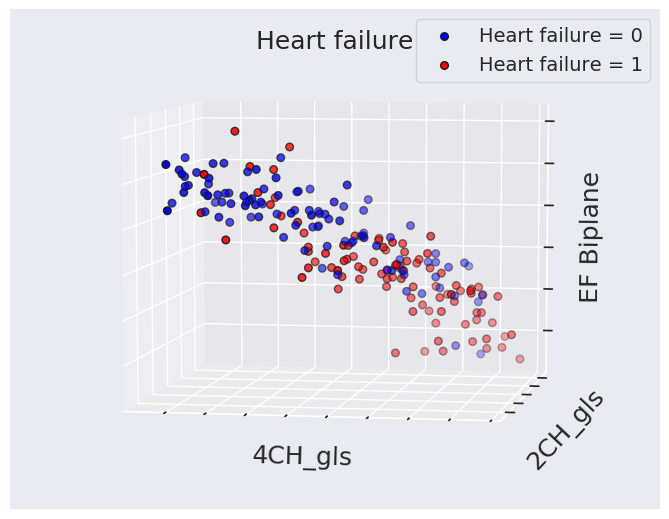
\includegraphics[width=0.99\textwidth]{results/scatter_gls_EF_hf.png}
        \caption{Heart failure.}
        \label{fig:scatter_gls_ef_hf}
    \end{subfigure}
    \begin{subfigure}[b]{0.49\textwidth}
        \centering
        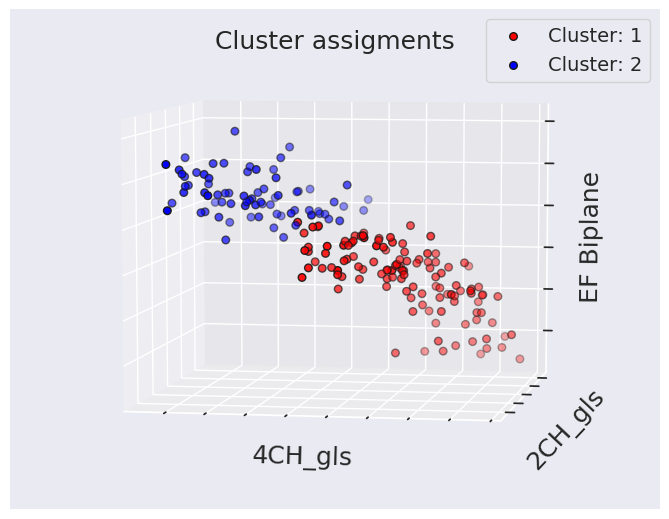
\includegraphics[width=0.99\textwidth]{results/scatter_gls_EF_ward2.png}
        \caption{\textit{Ward/2} cluster assignments.}
        \label{fig:scatter_gls_ef_ward2}
    \end{subfigure}\\
    \begin{subfigure}[b]{0.49\textwidth}
        \centering
        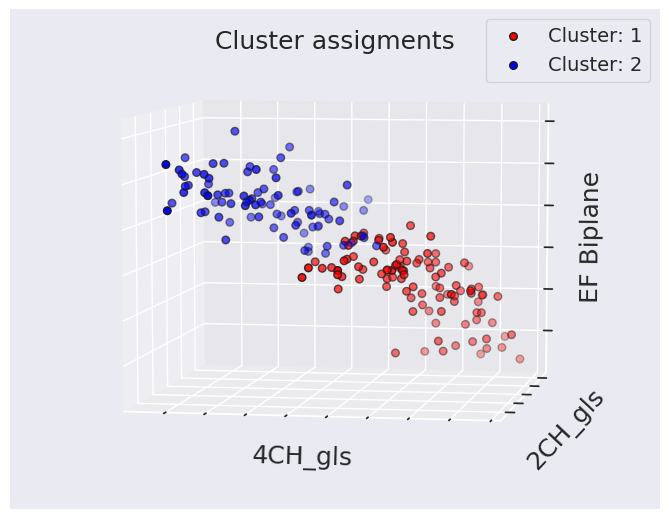
\includegraphics[width=0.99\textwidth]{results/scatter_gls_EF_complete2.png}
        \caption{\textit{Complete/2} cluster assignments.}
        \label{fig:scatter_gls_ef_complete2}
    \end{subfigure}
    \begin{subfigure}[b]{0.49\textwidth}
        \centering
        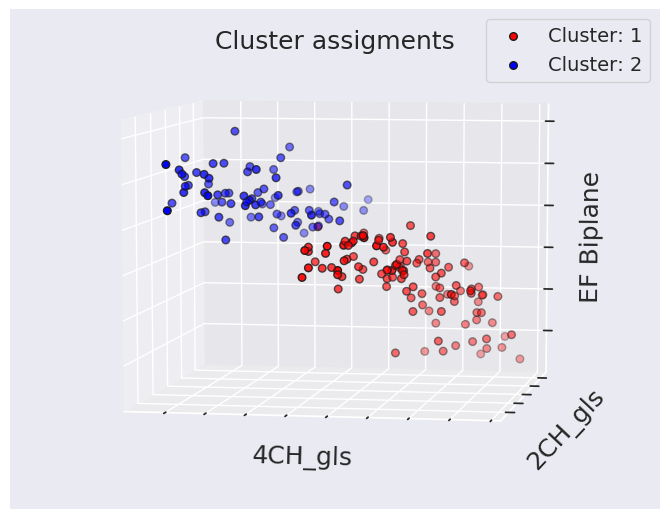
\includegraphics[width=0.99\textwidth]{results/scatter_gls_EF_average2.png}
        \caption{\textit{Average/2} cluster assignments.}
        \label{fig:scatter_gls_ef_average2}
    \end{subfigure}
    \caption{Scatterplot of peak GLS values in each view. Colors in the of the different dots are given by heart failure diagnosis, and cluster assignments of 
             ward/2, complete/2 and average/2 methods. Numbers are not included on the axes because the point of the figure is to illustrate the separability 
             of clusters, and heart failure.}
             \label{fig:scatter_gls_ef_hf_cluster_assignments}
\end{figure}

In figure \ref{fig:scatter_gls_ef_hf_cluster_assignments} scatterplots patients are plotted with the dimensions: 4-chamber peak systolic GLS, 2-chamber peak systolic GLS and EF. 
The colors of the points correspond to wheather the patient has heart failure or not, and which cluster the points belong to.
The plots are actually a lower dimensional projection of the GLS-EF peak-value dataset. 
This particular projection was chosen as it was found to be the projection where heart failure patients were as separable as possible. 
From plots \ref{fig:scatter_gls_ef_hf_cluster_assignments}b-d one can see that the clusters are fairly separable, 
heart failure on the other hand is not as easy to separate in these dimensions as can be seen in plot \ref{fig:scatter_gls_ef_average2}. 
\textit{Ward/2} and \textit{Complete/2} can in some sense be considered as binary classifiers where values under a certain threshold are categorized as heart failure.
The \textit{ward/2} method has the highest threshold for what is considered heart failure, and \textit{complete/2} has the lowest, 
which explains their difference in sensitivity and specificity score. 
From figure \ref{fig:pvc_hf_ari} one can see that the many of the ARI of PVC methods for classifying heart failure are close to zero, but substantially more of the methods score above zero in ARI
than the TSC methods, as can be seen by a comparison of figure \ref{fig:tsc_hf_ari} and \ref{fig:pvc_hf_ari}. Table \ref{tab:pvc_hf_ari} shows that the three highest ARIs are attained by the same
three methods that acheived the highest DORs. This means that there are most likely no methods evaluated at a higher number of cluster centers that will outperform \textit{ward/2},
or \textit{complete/2} at classifying heart failure. In addition, the conclusion will be that \textit{complete/2} is the best performing PVC method when classifying heart failure, 
since it has the highest overall accuracy (76$\%$), highest ARI (0.27), and second highest DOR (10.85). 

\begin{figure}[htb]
    \centering
    % \includegraphics[width=\textwidth]{results/pvc_hf_ari.png}
    %% Creator: Matplotlib, PGF backend
%%
%% To include the figure in your LaTeX document, write
%%   \input{<filename>.pgf}
%%
%% Make sure the required packages are loaded in your preamble
%%   \usepackage{pgf}
%%
%% Figures using additional raster images can only be included by \input if
%% they are in the same directory as the main LaTeX file. For loading figures
%% from other directories you can use the `import` package
%%   \usepackage{import}
%% and then include the figures with
%%   \import{<path to file>}{<filename>.pgf}
%%
%% Matplotlib used the following preamble
%%
\begingroup%
\makeatletter%
\begin{pgfpicture}%
\pgfpathrectangle{\pgfpointorigin}{\pgfqpoint{6.340000in}{2.340000in}}%
\pgfusepath{use as bounding box, clip}%
\begin{pgfscope}%
\pgfsetbuttcap%
\pgfsetmiterjoin%
\definecolor{currentfill}{rgb}{1.000000,1.000000,1.000000}%
\pgfsetfillcolor{currentfill}%
\pgfsetlinewidth{0.000000pt}%
\definecolor{currentstroke}{rgb}{1.000000,1.000000,1.000000}%
\pgfsetstrokecolor{currentstroke}%
\pgfsetdash{}{0pt}%
\pgfpathmoveto{\pgfqpoint{0.000000in}{-0.000000in}}%
\pgfpathlineto{\pgfqpoint{6.340000in}{-0.000000in}}%
\pgfpathlineto{\pgfqpoint{6.340000in}{2.340000in}}%
\pgfpathlineto{\pgfqpoint{0.000000in}{2.340000in}}%
\pgfpathclose%
\pgfusepath{fill}%
\end{pgfscope}%
\begin{pgfscope}%
\pgfsetbuttcap%
\pgfsetmiterjoin%
\definecolor{currentfill}{rgb}{0.917647,0.917647,0.949020}%
\pgfsetfillcolor{currentfill}%
\pgfsetlinewidth{0.000000pt}%
\definecolor{currentstroke}{rgb}{0.000000,0.000000,0.000000}%
\pgfsetstrokecolor{currentstroke}%
\pgfsetstrokeopacity{0.000000}%
\pgfsetdash{}{0pt}%
\pgfpathmoveto{\pgfqpoint{0.574769in}{0.557870in}}%
\pgfpathlineto{\pgfqpoint{6.240000in}{0.557870in}}%
\pgfpathlineto{\pgfqpoint{6.240000in}{2.240000in}}%
\pgfpathlineto{\pgfqpoint{0.574769in}{2.240000in}}%
\pgfpathclose%
\pgfusepath{fill}%
\end{pgfscope}%
\begin{pgfscope}%
\pgfpathrectangle{\pgfqpoint{0.574769in}{0.557870in}}{\pgfqpoint{5.665231in}{1.682130in}}%
\pgfusepath{clip}%
\pgfsetroundcap%
\pgfsetroundjoin%
\pgfsetlinewidth{1.003750pt}%
\definecolor{currentstroke}{rgb}{1.000000,1.000000,1.000000}%
\pgfsetstrokecolor{currentstroke}%
\pgfsetdash{}{0pt}%
\pgfpathmoveto{\pgfqpoint{0.889412in}{0.557870in}}%
\pgfpathlineto{\pgfqpoint{0.889412in}{2.240000in}}%
\pgfusepath{stroke}%
\end{pgfscope}%
\begin{pgfscope}%
\definecolor{textcolor}{rgb}{0.150000,0.150000,0.150000}%
\pgfsetstrokecolor{textcolor}%
\pgfsetfillcolor{textcolor}%
\pgftext[x=0.889412in,y=0.425926in,,top]{\color{textcolor}\sffamily\fontsize{11.000000}{13.200000}\selectfont \(\displaystyle 0.00\)}%
\end{pgfscope}%
\begin{pgfscope}%
\pgfpathrectangle{\pgfqpoint{0.574769in}{0.557870in}}{\pgfqpoint{5.665231in}{1.682130in}}%
\pgfusepath{clip}%
\pgfsetroundcap%
\pgfsetroundjoin%
\pgfsetlinewidth{1.003750pt}%
\definecolor{currentstroke}{rgb}{1.000000,1.000000,1.000000}%
\pgfsetstrokecolor{currentstroke}%
\pgfsetdash{}{0pt}%
\pgfpathmoveto{\pgfqpoint{1.823256in}{0.557870in}}%
\pgfpathlineto{\pgfqpoint{1.823256in}{2.240000in}}%
\pgfusepath{stroke}%
\end{pgfscope}%
\begin{pgfscope}%
\definecolor{textcolor}{rgb}{0.150000,0.150000,0.150000}%
\pgfsetstrokecolor{textcolor}%
\pgfsetfillcolor{textcolor}%
\pgftext[x=1.823256in,y=0.425926in,,top]{\color{textcolor}\sffamily\fontsize{11.000000}{13.200000}\selectfont \(\displaystyle 0.05\)}%
\end{pgfscope}%
\begin{pgfscope}%
\pgfpathrectangle{\pgfqpoint{0.574769in}{0.557870in}}{\pgfqpoint{5.665231in}{1.682130in}}%
\pgfusepath{clip}%
\pgfsetroundcap%
\pgfsetroundjoin%
\pgfsetlinewidth{1.003750pt}%
\definecolor{currentstroke}{rgb}{1.000000,1.000000,1.000000}%
\pgfsetstrokecolor{currentstroke}%
\pgfsetdash{}{0pt}%
\pgfpathmoveto{\pgfqpoint{2.757101in}{0.557870in}}%
\pgfpathlineto{\pgfqpoint{2.757101in}{2.240000in}}%
\pgfusepath{stroke}%
\end{pgfscope}%
\begin{pgfscope}%
\definecolor{textcolor}{rgb}{0.150000,0.150000,0.150000}%
\pgfsetstrokecolor{textcolor}%
\pgfsetfillcolor{textcolor}%
\pgftext[x=2.757101in,y=0.425926in,,top]{\color{textcolor}\sffamily\fontsize{11.000000}{13.200000}\selectfont \(\displaystyle 0.10\)}%
\end{pgfscope}%
\begin{pgfscope}%
\pgfpathrectangle{\pgfqpoint{0.574769in}{0.557870in}}{\pgfqpoint{5.665231in}{1.682130in}}%
\pgfusepath{clip}%
\pgfsetroundcap%
\pgfsetroundjoin%
\pgfsetlinewidth{1.003750pt}%
\definecolor{currentstroke}{rgb}{1.000000,1.000000,1.000000}%
\pgfsetstrokecolor{currentstroke}%
\pgfsetdash{}{0pt}%
\pgfpathmoveto{\pgfqpoint{3.690945in}{0.557870in}}%
\pgfpathlineto{\pgfqpoint{3.690945in}{2.240000in}}%
\pgfusepath{stroke}%
\end{pgfscope}%
\begin{pgfscope}%
\definecolor{textcolor}{rgb}{0.150000,0.150000,0.150000}%
\pgfsetstrokecolor{textcolor}%
\pgfsetfillcolor{textcolor}%
\pgftext[x=3.690945in,y=0.425926in,,top]{\color{textcolor}\sffamily\fontsize{11.000000}{13.200000}\selectfont \(\displaystyle 0.15\)}%
\end{pgfscope}%
\begin{pgfscope}%
\pgfpathrectangle{\pgfqpoint{0.574769in}{0.557870in}}{\pgfqpoint{5.665231in}{1.682130in}}%
\pgfusepath{clip}%
\pgfsetroundcap%
\pgfsetroundjoin%
\pgfsetlinewidth{1.003750pt}%
\definecolor{currentstroke}{rgb}{1.000000,1.000000,1.000000}%
\pgfsetstrokecolor{currentstroke}%
\pgfsetdash{}{0pt}%
\pgfpathmoveto{\pgfqpoint{4.624789in}{0.557870in}}%
\pgfpathlineto{\pgfqpoint{4.624789in}{2.240000in}}%
\pgfusepath{stroke}%
\end{pgfscope}%
\begin{pgfscope}%
\definecolor{textcolor}{rgb}{0.150000,0.150000,0.150000}%
\pgfsetstrokecolor{textcolor}%
\pgfsetfillcolor{textcolor}%
\pgftext[x=4.624789in,y=0.425926in,,top]{\color{textcolor}\sffamily\fontsize{11.000000}{13.200000}\selectfont \(\displaystyle 0.20\)}%
\end{pgfscope}%
\begin{pgfscope}%
\pgfpathrectangle{\pgfqpoint{0.574769in}{0.557870in}}{\pgfqpoint{5.665231in}{1.682130in}}%
\pgfusepath{clip}%
\pgfsetroundcap%
\pgfsetroundjoin%
\pgfsetlinewidth{1.003750pt}%
\definecolor{currentstroke}{rgb}{1.000000,1.000000,1.000000}%
\pgfsetstrokecolor{currentstroke}%
\pgfsetdash{}{0pt}%
\pgfpathmoveto{\pgfqpoint{5.558633in}{0.557870in}}%
\pgfpathlineto{\pgfqpoint{5.558633in}{2.240000in}}%
\pgfusepath{stroke}%
\end{pgfscope}%
\begin{pgfscope}%
\definecolor{textcolor}{rgb}{0.150000,0.150000,0.150000}%
\pgfsetstrokecolor{textcolor}%
\pgfsetfillcolor{textcolor}%
\pgftext[x=5.558633in,y=0.425926in,,top]{\color{textcolor}\sffamily\fontsize{11.000000}{13.200000}\selectfont \(\displaystyle 0.25\)}%
\end{pgfscope}%
\begin{pgfscope}%
\definecolor{textcolor}{rgb}{0.150000,0.150000,0.150000}%
\pgfsetstrokecolor{textcolor}%
\pgfsetfillcolor{textcolor}%
\pgftext[x=3.407384in,y=0.235185in,,top]{\color{textcolor}\sffamily\fontsize{11.000000}{13.200000}\selectfont ARI}%
\end{pgfscope}%
\begin{pgfscope}%
\pgfpathrectangle{\pgfqpoint{0.574769in}{0.557870in}}{\pgfqpoint{5.665231in}{1.682130in}}%
\pgfusepath{clip}%
\pgfsetroundcap%
\pgfsetroundjoin%
\pgfsetlinewidth{1.003750pt}%
\definecolor{currentstroke}{rgb}{1.000000,1.000000,1.000000}%
\pgfsetstrokecolor{currentstroke}%
\pgfsetdash{}{0pt}%
\pgfpathmoveto{\pgfqpoint{0.574769in}{0.557870in}}%
\pgfpathlineto{\pgfqpoint{6.240000in}{0.557870in}}%
\pgfusepath{stroke}%
\end{pgfscope}%
\begin{pgfscope}%
\definecolor{textcolor}{rgb}{0.150000,0.150000,0.150000}%
\pgfsetstrokecolor{textcolor}%
\pgfsetfillcolor{textcolor}%
\pgftext[x=0.366783in,y=0.505064in,left,base]{\color{textcolor}\sffamily\fontsize{11.000000}{13.200000}\selectfont \(\displaystyle 0\)}%
\end{pgfscope}%
\begin{pgfscope}%
\pgfpathrectangle{\pgfqpoint{0.574769in}{0.557870in}}{\pgfqpoint{5.665231in}{1.682130in}}%
\pgfusepath{clip}%
\pgfsetroundcap%
\pgfsetroundjoin%
\pgfsetlinewidth{1.003750pt}%
\definecolor{currentstroke}{rgb}{1.000000,1.000000,1.000000}%
\pgfsetstrokecolor{currentstroke}%
\pgfsetdash{}{0pt}%
\pgfpathmoveto{\pgfqpoint{0.574769in}{0.963447in}}%
\pgfpathlineto{\pgfqpoint{6.240000in}{0.963447in}}%
\pgfusepath{stroke}%
\end{pgfscope}%
\begin{pgfscope}%
\definecolor{textcolor}{rgb}{0.150000,0.150000,0.150000}%
\pgfsetstrokecolor{textcolor}%
\pgfsetfillcolor{textcolor}%
\pgftext[x=0.290741in,y=0.910640in,left,base]{\color{textcolor}\sffamily\fontsize{11.000000}{13.200000}\selectfont \(\displaystyle 20\)}%
\end{pgfscope}%
\begin{pgfscope}%
\pgfpathrectangle{\pgfqpoint{0.574769in}{0.557870in}}{\pgfqpoint{5.665231in}{1.682130in}}%
\pgfusepath{clip}%
\pgfsetroundcap%
\pgfsetroundjoin%
\pgfsetlinewidth{1.003750pt}%
\definecolor{currentstroke}{rgb}{1.000000,1.000000,1.000000}%
\pgfsetstrokecolor{currentstroke}%
\pgfsetdash{}{0pt}%
\pgfpathmoveto{\pgfqpoint{0.574769in}{1.369024in}}%
\pgfpathlineto{\pgfqpoint{6.240000in}{1.369024in}}%
\pgfusepath{stroke}%
\end{pgfscope}%
\begin{pgfscope}%
\definecolor{textcolor}{rgb}{0.150000,0.150000,0.150000}%
\pgfsetstrokecolor{textcolor}%
\pgfsetfillcolor{textcolor}%
\pgftext[x=0.290741in,y=1.316217in,left,base]{\color{textcolor}\sffamily\fontsize{11.000000}{13.200000}\selectfont \(\displaystyle 40\)}%
\end{pgfscope}%
\begin{pgfscope}%
\pgfpathrectangle{\pgfqpoint{0.574769in}{0.557870in}}{\pgfqpoint{5.665231in}{1.682130in}}%
\pgfusepath{clip}%
\pgfsetroundcap%
\pgfsetroundjoin%
\pgfsetlinewidth{1.003750pt}%
\definecolor{currentstroke}{rgb}{1.000000,1.000000,1.000000}%
\pgfsetstrokecolor{currentstroke}%
\pgfsetdash{}{0pt}%
\pgfpathmoveto{\pgfqpoint{0.574769in}{1.774601in}}%
\pgfpathlineto{\pgfqpoint{6.240000in}{1.774601in}}%
\pgfusepath{stroke}%
\end{pgfscope}%
\begin{pgfscope}%
\definecolor{textcolor}{rgb}{0.150000,0.150000,0.150000}%
\pgfsetstrokecolor{textcolor}%
\pgfsetfillcolor{textcolor}%
\pgftext[x=0.290741in,y=1.721794in,left,base]{\color{textcolor}\sffamily\fontsize{11.000000}{13.200000}\selectfont \(\displaystyle 60\)}%
\end{pgfscope}%
\begin{pgfscope}%
\pgfpathrectangle{\pgfqpoint{0.574769in}{0.557870in}}{\pgfqpoint{5.665231in}{1.682130in}}%
\pgfusepath{clip}%
\pgfsetroundcap%
\pgfsetroundjoin%
\pgfsetlinewidth{1.003750pt}%
\definecolor{currentstroke}{rgb}{1.000000,1.000000,1.000000}%
\pgfsetstrokecolor{currentstroke}%
\pgfsetdash{}{0pt}%
\pgfpathmoveto{\pgfqpoint{0.574769in}{2.180177in}}%
\pgfpathlineto{\pgfqpoint{6.240000in}{2.180177in}}%
\pgfusepath{stroke}%
\end{pgfscope}%
\begin{pgfscope}%
\definecolor{textcolor}{rgb}{0.150000,0.150000,0.150000}%
\pgfsetstrokecolor{textcolor}%
\pgfsetfillcolor{textcolor}%
\pgftext[x=0.290741in,y=2.127371in,left,base]{\color{textcolor}\sffamily\fontsize{11.000000}{13.200000}\selectfont \(\displaystyle 80\)}%
\end{pgfscope}%
\begin{pgfscope}%
\definecolor{textcolor}{rgb}{0.150000,0.150000,0.150000}%
\pgfsetstrokecolor{textcolor}%
\pgfsetfillcolor{textcolor}%
\pgftext[x=0.235185in,y=1.398935in,,bottom,rotate=90.000000]{\color{textcolor}\sffamily\fontsize{11.000000}{13.200000}\selectfont Occurance}%
\end{pgfscope}%
\begin{pgfscope}%
\pgfpathrectangle{\pgfqpoint{0.574769in}{0.557870in}}{\pgfqpoint{5.665231in}{1.682130in}}%
\pgfusepath{clip}%
\pgfsetbuttcap%
\pgfsetmiterjoin%
\definecolor{currentfill}{rgb}{0.298039,0.447059,0.690196}%
\pgfsetfillcolor{currentfill}%
\pgfsetfillopacity{0.400000}%
\pgfsetlinewidth{1.003750pt}%
\definecolor{currentstroke}{rgb}{1.000000,1.000000,1.000000}%
\pgfsetstrokecolor{currentstroke}%
\pgfsetstrokeopacity{0.400000}%
\pgfsetdash{}{0pt}%
\pgfpathmoveto{\pgfqpoint{0.832279in}{0.557870in}}%
\pgfpathlineto{\pgfqpoint{1.568023in}{0.557870in}}%
\pgfpathlineto{\pgfqpoint{1.568023in}{2.159899in}}%
\pgfpathlineto{\pgfqpoint{0.832279in}{2.159899in}}%
\pgfpathclose%
\pgfusepath{stroke,fill}%
\end{pgfscope}%
\begin{pgfscope}%
\pgfpathrectangle{\pgfqpoint{0.574769in}{0.557870in}}{\pgfqpoint{5.665231in}{1.682130in}}%
\pgfusepath{clip}%
\pgfsetbuttcap%
\pgfsetmiterjoin%
\definecolor{currentfill}{rgb}{0.298039,0.447059,0.690196}%
\pgfsetfillcolor{currentfill}%
\pgfsetfillopacity{0.400000}%
\pgfsetlinewidth{1.003750pt}%
\definecolor{currentstroke}{rgb}{1.000000,1.000000,1.000000}%
\pgfsetstrokecolor{currentstroke}%
\pgfsetstrokeopacity{0.400000}%
\pgfsetdash{}{0pt}%
\pgfpathmoveto{\pgfqpoint{1.568023in}{0.557870in}}%
\pgfpathlineto{\pgfqpoint{2.303768in}{0.557870in}}%
\pgfpathlineto{\pgfqpoint{2.303768in}{0.943168in}}%
\pgfpathlineto{\pgfqpoint{1.568023in}{0.943168in}}%
\pgfpathclose%
\pgfusepath{stroke,fill}%
\end{pgfscope}%
\begin{pgfscope}%
\pgfpathrectangle{\pgfqpoint{0.574769in}{0.557870in}}{\pgfqpoint{5.665231in}{1.682130in}}%
\pgfusepath{clip}%
\pgfsetbuttcap%
\pgfsetmiterjoin%
\definecolor{currentfill}{rgb}{0.298039,0.447059,0.690196}%
\pgfsetfillcolor{currentfill}%
\pgfsetfillopacity{0.400000}%
\pgfsetlinewidth{1.003750pt}%
\definecolor{currentstroke}{rgb}{1.000000,1.000000,1.000000}%
\pgfsetstrokecolor{currentstroke}%
\pgfsetstrokeopacity{0.400000}%
\pgfsetdash{}{0pt}%
\pgfpathmoveto{\pgfqpoint{2.303768in}{0.557870in}}%
\pgfpathlineto{\pgfqpoint{3.039512in}{0.557870in}}%
\pgfpathlineto{\pgfqpoint{3.039512in}{1.632649in}}%
\pgfpathlineto{\pgfqpoint{2.303768in}{1.632649in}}%
\pgfpathclose%
\pgfusepath{stroke,fill}%
\end{pgfscope}%
\begin{pgfscope}%
\pgfpathrectangle{\pgfqpoint{0.574769in}{0.557870in}}{\pgfqpoint{5.665231in}{1.682130in}}%
\pgfusepath{clip}%
\pgfsetbuttcap%
\pgfsetmiterjoin%
\definecolor{currentfill}{rgb}{0.298039,0.447059,0.690196}%
\pgfsetfillcolor{currentfill}%
\pgfsetfillopacity{0.400000}%
\pgfsetlinewidth{1.003750pt}%
\definecolor{currentstroke}{rgb}{1.000000,1.000000,1.000000}%
\pgfsetstrokecolor{currentstroke}%
\pgfsetstrokeopacity{0.400000}%
\pgfsetdash{}{0pt}%
\pgfpathmoveto{\pgfqpoint{3.039512in}{0.557870in}}%
\pgfpathlineto{\pgfqpoint{3.775256in}{0.557870in}}%
\pgfpathlineto{\pgfqpoint{3.775256in}{1.267630in}}%
\pgfpathlineto{\pgfqpoint{3.039512in}{1.267630in}}%
\pgfpathclose%
\pgfusepath{stroke,fill}%
\end{pgfscope}%
\begin{pgfscope}%
\pgfpathrectangle{\pgfqpoint{0.574769in}{0.557870in}}{\pgfqpoint{5.665231in}{1.682130in}}%
\pgfusepath{clip}%
\pgfsetbuttcap%
\pgfsetmiterjoin%
\definecolor{currentfill}{rgb}{0.298039,0.447059,0.690196}%
\pgfsetfillcolor{currentfill}%
\pgfsetfillopacity{0.400000}%
\pgfsetlinewidth{1.003750pt}%
\definecolor{currentstroke}{rgb}{1.000000,1.000000,1.000000}%
\pgfsetstrokecolor{currentstroke}%
\pgfsetstrokeopacity{0.400000}%
\pgfsetdash{}{0pt}%
\pgfpathmoveto{\pgfqpoint{3.775256in}{0.557870in}}%
\pgfpathlineto{\pgfqpoint{4.511001in}{0.557870in}}%
\pgfpathlineto{\pgfqpoint{4.511001in}{1.004005in}}%
\pgfpathlineto{\pgfqpoint{3.775256in}{1.004005in}}%
\pgfpathclose%
\pgfusepath{stroke,fill}%
\end{pgfscope}%
\begin{pgfscope}%
\pgfpathrectangle{\pgfqpoint{0.574769in}{0.557870in}}{\pgfqpoint{5.665231in}{1.682130in}}%
\pgfusepath{clip}%
\pgfsetbuttcap%
\pgfsetmiterjoin%
\definecolor{currentfill}{rgb}{0.298039,0.447059,0.690196}%
\pgfsetfillcolor{currentfill}%
\pgfsetfillopacity{0.400000}%
\pgfsetlinewidth{1.003750pt}%
\definecolor{currentstroke}{rgb}{1.000000,1.000000,1.000000}%
\pgfsetstrokecolor{currentstroke}%
\pgfsetstrokeopacity{0.400000}%
\pgfsetdash{}{0pt}%
\pgfpathmoveto{\pgfqpoint{4.511001in}{0.557870in}}%
\pgfpathlineto{\pgfqpoint{5.246745in}{0.557870in}}%
\pgfpathlineto{\pgfqpoint{5.246745in}{0.659264in}}%
\pgfpathlineto{\pgfqpoint{4.511001in}{0.659264in}}%
\pgfpathclose%
\pgfusepath{stroke,fill}%
\end{pgfscope}%
\begin{pgfscope}%
\pgfpathrectangle{\pgfqpoint{0.574769in}{0.557870in}}{\pgfqpoint{5.665231in}{1.682130in}}%
\pgfusepath{clip}%
\pgfsetbuttcap%
\pgfsetmiterjoin%
\definecolor{currentfill}{rgb}{0.298039,0.447059,0.690196}%
\pgfsetfillcolor{currentfill}%
\pgfsetfillopacity{0.400000}%
\pgfsetlinewidth{1.003750pt}%
\definecolor{currentstroke}{rgb}{1.000000,1.000000,1.000000}%
\pgfsetstrokecolor{currentstroke}%
\pgfsetstrokeopacity{0.400000}%
\pgfsetdash{}{0pt}%
\pgfpathmoveto{\pgfqpoint{5.246745in}{0.557870in}}%
\pgfpathlineto{\pgfqpoint{5.982489in}{0.557870in}}%
\pgfpathlineto{\pgfqpoint{5.982489in}{0.618707in}}%
\pgfpathlineto{\pgfqpoint{5.246745in}{0.618707in}}%
\pgfpathclose%
\pgfusepath{stroke,fill}%
\end{pgfscope}%
\begin{pgfscope}%
\pgfsetrectcap%
\pgfsetmiterjoin%
\pgfsetlinewidth{1.254687pt}%
\definecolor{currentstroke}{rgb}{1.000000,1.000000,1.000000}%
\pgfsetstrokecolor{currentstroke}%
\pgfsetdash{}{0pt}%
\pgfpathmoveto{\pgfqpoint{0.574769in}{0.557870in}}%
\pgfpathlineto{\pgfqpoint{0.574769in}{2.240000in}}%
\pgfusepath{stroke}%
\end{pgfscope}%
\begin{pgfscope}%
\pgfsetrectcap%
\pgfsetmiterjoin%
\pgfsetlinewidth{1.254687pt}%
\definecolor{currentstroke}{rgb}{1.000000,1.000000,1.000000}%
\pgfsetstrokecolor{currentstroke}%
\pgfsetdash{}{0pt}%
\pgfpathmoveto{\pgfqpoint{6.240000in}{0.557870in}}%
\pgfpathlineto{\pgfqpoint{6.240000in}{2.240000in}}%
\pgfusepath{stroke}%
\end{pgfscope}%
\begin{pgfscope}%
\pgfsetrectcap%
\pgfsetmiterjoin%
\pgfsetlinewidth{1.254687pt}%
\definecolor{currentstroke}{rgb}{1.000000,1.000000,1.000000}%
\pgfsetstrokecolor{currentstroke}%
\pgfsetdash{}{0pt}%
\pgfpathmoveto{\pgfqpoint{0.574769in}{0.557870in}}%
\pgfpathlineto{\pgfqpoint{6.240000in}{0.557870in}}%
\pgfusepath{stroke}%
\end{pgfscope}%
\begin{pgfscope}%
\pgfsetrectcap%
\pgfsetmiterjoin%
\pgfsetlinewidth{1.254687pt}%
\definecolor{currentstroke}{rgb}{1.000000,1.000000,1.000000}%
\pgfsetstrokecolor{currentstroke}%
\pgfsetdash{}{0pt}%
\pgfpathmoveto{\pgfqpoint{0.574769in}{2.240000in}}%
\pgfpathlineto{\pgfqpoint{6.240000in}{2.240000in}}%
\pgfusepath{stroke}%
\end{pgfscope}%
\end{pgfpicture}%
\makeatother%
\endgroup%

    \caption{Distribution plot of ARI of all PVC methods evaluated at $\{2,9\}$ cluster centers when applied to classify heart failure.}
    \label{fig:pvc_hf_ari}
\end{figure}

\begin{table*}[htb]
    \centering
    \ra{1.3}
    \begin{tabular}{lr}
        \toprule
        Dataset-Method    &  ARI \\
        \midrule
        gls-EF/complete/2 & 0.27 \\
        gls-EF/ward/2     & 0.24 \\
        gls-EF/average/2  & 0.24 \\
        rls-EF/complete/2 & 0.21 \\
        gls-EF/complete/3 & 0.21 \\
        \bottomrule
    \end{tabular}
    \caption{The five highest ARI scores attained when applying PVC for detecting heart failure.
             The \textbf{Dataset-Method} column indicates \textit{Dataset used}$/$\textit{Linkage criteria of method}$/$\textit{Number of cluster centers}.}
    \label{tab:pvc_hf_ari}
\end{table*}

\newpage 

\subsection{Deep Neural Network}

From the distribution plot in figure \ref{fig:dl_hf_dor_sens_spec_dist}a one can see that the most frequent DOR by the NN models is zero when training them to predict heart failure.
In the scatterplot in figure \ref{fig:dl_hf_dor_sens_spec_dist}b one can see that sensitivity scores vary between $0.15$ and $0.65$, and the specificity scores vary between $0$ and $0.68$.
The highest DOR of $1.36$ is attained by using only the GLS curve from the 4-chamber view as input, as can be seen from table \ref{tab:dl_hf_dor_sens_spec_dist}.
In fact the five highest DORs attained by NN models trained to classify heart failure are acheived using only curves from a single view as input.
There does not seem to be a particular view that is favored, as 4-chamber view, 2-chamber view and apical-view are are all found in the NN variations in table \ref{tab:dl_hf_dor_sens_spec_dist}.
The overall accuracy of the model variations are also fairly low, $0.54$ being the highest accuracy acheived.
Since the heart failure dataset is fairly evenly distribution (recall figure \ref{fig:hf_ind_dist}) an accuracy of $0.54$ is not much better than what could be acheived 
by randomly guessing the label.

\begin{figure}[htb]
    \centering
    % \includegraphics[width=\textwidth]{results/dl_hf_dor_sens_spec_dist.png}
    %% Creator: Matplotlib, PGF backend
%%
%% To include the figure in your LaTeX document, write
%%   \input{<filename>.pgf}
%%
%% Make sure the required packages are loaded in your preamble
%%   \usepackage{pgf}
%%
%% Figures using additional raster images can only be included by \input if
%% they are in the same directory as the main LaTeX file. For loading figures
%% from other directories you can use the `import` package
%%   \usepackage{import}
%% and then include the figures with
%%   \import{<path to file>}{<filename>.pgf}
%%
%% Matplotlib used the following preamble
%%
\begingroup%
\makeatletter%
\begin{pgfpicture}%
\pgfpathrectangle{\pgfpointorigin}{\pgfqpoint{6.246672in}{2.340000in}}%
\pgfusepath{use as bounding box, clip}%
\begin{pgfscope}%
\pgfsetbuttcap%
\pgfsetmiterjoin%
\definecolor{currentfill}{rgb}{1.000000,1.000000,1.000000}%
\pgfsetfillcolor{currentfill}%
\pgfsetlinewidth{0.000000pt}%
\definecolor{currentstroke}{rgb}{1.000000,1.000000,1.000000}%
\pgfsetstrokecolor{currentstroke}%
\pgfsetdash{}{0pt}%
\pgfpathmoveto{\pgfqpoint{0.000000in}{-0.000000in}}%
\pgfpathlineto{\pgfqpoint{6.246672in}{-0.000000in}}%
\pgfpathlineto{\pgfqpoint{6.246672in}{2.340000in}}%
\pgfpathlineto{\pgfqpoint{0.000000in}{2.340000in}}%
\pgfpathclose%
\pgfusepath{fill}%
\end{pgfscope}%
\begin{pgfscope}%
\pgfsetbuttcap%
\pgfsetmiterjoin%
\definecolor{currentfill}{rgb}{0.917647,0.917647,0.949020}%
\pgfsetfillcolor{currentfill}%
\pgfsetlinewidth{0.000000pt}%
\definecolor{currentstroke}{rgb}{0.000000,0.000000,0.000000}%
\pgfsetstrokecolor{currentstroke}%
\pgfsetstrokeopacity{0.000000}%
\pgfsetdash{}{0pt}%
\pgfpathmoveto{\pgfqpoint{0.574769in}{0.557870in}}%
\pgfpathlineto{\pgfqpoint{2.999734in}{0.557870in}}%
\pgfpathlineto{\pgfqpoint{2.999734in}{2.042604in}}%
\pgfpathlineto{\pgfqpoint{0.574769in}{2.042604in}}%
\pgfpathclose%
\pgfusepath{fill}%
\end{pgfscope}%
\begin{pgfscope}%
\pgfpathrectangle{\pgfqpoint{0.574769in}{0.557870in}}{\pgfqpoint{2.424965in}{1.484734in}}%
\pgfusepath{clip}%
\pgfsetroundcap%
\pgfsetroundjoin%
\pgfsetlinewidth{1.003750pt}%
\definecolor{currentstroke}{rgb}{1.000000,1.000000,1.000000}%
\pgfsetstrokecolor{currentstroke}%
\pgfsetdash{}{0pt}%
\pgfpathmoveto{\pgfqpoint{0.684994in}{0.557870in}}%
\pgfpathlineto{\pgfqpoint{0.684994in}{2.042604in}}%
\pgfusepath{stroke}%
\end{pgfscope}%
\begin{pgfscope}%
\definecolor{textcolor}{rgb}{0.150000,0.150000,0.150000}%
\pgfsetstrokecolor{textcolor}%
\pgfsetfillcolor{textcolor}%
\pgftext[x=0.684994in,y=0.425926in,,top]{\color{textcolor}\sffamily\fontsize{11.000000}{13.200000}\selectfont \(\displaystyle 0.0\)}%
\end{pgfscope}%
\begin{pgfscope}%
\pgfpathrectangle{\pgfqpoint{0.574769in}{0.557870in}}{\pgfqpoint{2.424965in}{1.484734in}}%
\pgfusepath{clip}%
\pgfsetroundcap%
\pgfsetroundjoin%
\pgfsetlinewidth{1.003750pt}%
\definecolor{currentstroke}{rgb}{1.000000,1.000000,1.000000}%
\pgfsetstrokecolor{currentstroke}%
\pgfsetdash{}{0pt}%
\pgfpathmoveto{\pgfqpoint{1.496956in}{0.557870in}}%
\pgfpathlineto{\pgfqpoint{1.496956in}{2.042604in}}%
\pgfusepath{stroke}%
\end{pgfscope}%
\begin{pgfscope}%
\definecolor{textcolor}{rgb}{0.150000,0.150000,0.150000}%
\pgfsetstrokecolor{textcolor}%
\pgfsetfillcolor{textcolor}%
\pgftext[x=1.496956in,y=0.425926in,,top]{\color{textcolor}\sffamily\fontsize{11.000000}{13.200000}\selectfont \(\displaystyle 0.5\)}%
\end{pgfscope}%
\begin{pgfscope}%
\pgfpathrectangle{\pgfqpoint{0.574769in}{0.557870in}}{\pgfqpoint{2.424965in}{1.484734in}}%
\pgfusepath{clip}%
\pgfsetroundcap%
\pgfsetroundjoin%
\pgfsetlinewidth{1.003750pt}%
\definecolor{currentstroke}{rgb}{1.000000,1.000000,1.000000}%
\pgfsetstrokecolor{currentstroke}%
\pgfsetdash{}{0pt}%
\pgfpathmoveto{\pgfqpoint{2.308918in}{0.557870in}}%
\pgfpathlineto{\pgfqpoint{2.308918in}{2.042604in}}%
\pgfusepath{stroke}%
\end{pgfscope}%
\begin{pgfscope}%
\definecolor{textcolor}{rgb}{0.150000,0.150000,0.150000}%
\pgfsetstrokecolor{textcolor}%
\pgfsetfillcolor{textcolor}%
\pgftext[x=2.308918in,y=0.425926in,,top]{\color{textcolor}\sffamily\fontsize{11.000000}{13.200000}\selectfont \(\displaystyle 1.0\)}%
\end{pgfscope}%
\begin{pgfscope}%
\definecolor{textcolor}{rgb}{0.150000,0.150000,0.150000}%
\pgfsetstrokecolor{textcolor}%
\pgfsetfillcolor{textcolor}%
\pgftext[x=1.787251in,y=0.235185in,,top]{\color{textcolor}\sffamily\fontsize{11.000000}{13.200000}\selectfont DOR}%
\end{pgfscope}%
\begin{pgfscope}%
\pgfpathrectangle{\pgfqpoint{0.574769in}{0.557870in}}{\pgfqpoint{2.424965in}{1.484734in}}%
\pgfusepath{clip}%
\pgfsetroundcap%
\pgfsetroundjoin%
\pgfsetlinewidth{1.003750pt}%
\definecolor{currentstroke}{rgb}{1.000000,1.000000,1.000000}%
\pgfsetstrokecolor{currentstroke}%
\pgfsetdash{}{0pt}%
\pgfpathmoveto{\pgfqpoint{0.574769in}{0.557870in}}%
\pgfpathlineto{\pgfqpoint{2.999734in}{0.557870in}}%
\pgfusepath{stroke}%
\end{pgfscope}%
\begin{pgfscope}%
\definecolor{textcolor}{rgb}{0.150000,0.150000,0.150000}%
\pgfsetstrokecolor{textcolor}%
\pgfsetfillcolor{textcolor}%
\pgftext[x=0.366783in,y=0.505064in,left,base]{\color{textcolor}\sffamily\fontsize{11.000000}{13.200000}\selectfont \(\displaystyle 0\)}%
\end{pgfscope}%
\begin{pgfscope}%
\pgfpathrectangle{\pgfqpoint{0.574769in}{0.557870in}}{\pgfqpoint{2.424965in}{1.484734in}}%
\pgfusepath{clip}%
\pgfsetroundcap%
\pgfsetroundjoin%
\pgfsetlinewidth{1.003750pt}%
\definecolor{currentstroke}{rgb}{1.000000,1.000000,1.000000}%
\pgfsetstrokecolor{currentstroke}%
\pgfsetdash{}{0pt}%
\pgfpathmoveto{\pgfqpoint{0.574769in}{1.101729in}}%
\pgfpathlineto{\pgfqpoint{2.999734in}{1.101729in}}%
\pgfusepath{stroke}%
\end{pgfscope}%
\begin{pgfscope}%
\definecolor{textcolor}{rgb}{0.150000,0.150000,0.150000}%
\pgfsetstrokecolor{textcolor}%
\pgfsetfillcolor{textcolor}%
\pgftext[x=0.366783in,y=1.048922in,left,base]{\color{textcolor}\sffamily\fontsize{11.000000}{13.200000}\selectfont \(\displaystyle 5\)}%
\end{pgfscope}%
\begin{pgfscope}%
\pgfpathrectangle{\pgfqpoint{0.574769in}{0.557870in}}{\pgfqpoint{2.424965in}{1.484734in}}%
\pgfusepath{clip}%
\pgfsetroundcap%
\pgfsetroundjoin%
\pgfsetlinewidth{1.003750pt}%
\definecolor{currentstroke}{rgb}{1.000000,1.000000,1.000000}%
\pgfsetstrokecolor{currentstroke}%
\pgfsetdash{}{0pt}%
\pgfpathmoveto{\pgfqpoint{0.574769in}{1.645587in}}%
\pgfpathlineto{\pgfqpoint{2.999734in}{1.645587in}}%
\pgfusepath{stroke}%
\end{pgfscope}%
\begin{pgfscope}%
\definecolor{textcolor}{rgb}{0.150000,0.150000,0.150000}%
\pgfsetstrokecolor{textcolor}%
\pgfsetfillcolor{textcolor}%
\pgftext[x=0.290741in,y=1.592781in,left,base]{\color{textcolor}\sffamily\fontsize{11.000000}{13.200000}\selectfont \(\displaystyle 10\)}%
\end{pgfscope}%
\begin{pgfscope}%
\definecolor{textcolor}{rgb}{0.150000,0.150000,0.150000}%
\pgfsetstrokecolor{textcolor}%
\pgfsetfillcolor{textcolor}%
\pgftext[x=0.235185in,y=1.300237in,,bottom,rotate=90.000000]{\color{textcolor}\sffamily\fontsize{11.000000}{13.200000}\selectfont Occurance}%
\end{pgfscope}%
\begin{pgfscope}%
\pgfpathrectangle{\pgfqpoint{0.574769in}{0.557870in}}{\pgfqpoint{2.424965in}{1.484734in}}%
\pgfusepath{clip}%
\pgfsetbuttcap%
\pgfsetmiterjoin%
\definecolor{currentfill}{rgb}{0.298039,0.447059,0.690196}%
\pgfsetfillcolor{currentfill}%
\pgfsetfillopacity{0.400000}%
\pgfsetlinewidth{1.003750pt}%
\definecolor{currentstroke}{rgb}{1.000000,1.000000,1.000000}%
\pgfsetstrokecolor{currentstroke}%
\pgfsetstrokeopacity{0.400000}%
\pgfsetdash{}{0pt}%
\pgfpathmoveto{\pgfqpoint{0.684994in}{0.557870in}}%
\pgfpathlineto{\pgfqpoint{0.905446in}{0.557870in}}%
\pgfpathlineto{\pgfqpoint{0.905446in}{1.971903in}}%
\pgfpathlineto{\pgfqpoint{0.684994in}{1.971903in}}%
\pgfpathclose%
\pgfusepath{stroke,fill}%
\end{pgfscope}%
\begin{pgfscope}%
\pgfpathrectangle{\pgfqpoint{0.574769in}{0.557870in}}{\pgfqpoint{2.424965in}{1.484734in}}%
\pgfusepath{clip}%
\pgfsetbuttcap%
\pgfsetmiterjoin%
\definecolor{currentfill}{rgb}{0.298039,0.447059,0.690196}%
\pgfsetfillcolor{currentfill}%
\pgfsetfillopacity{0.400000}%
\pgfsetlinewidth{1.003750pt}%
\definecolor{currentstroke}{rgb}{1.000000,1.000000,1.000000}%
\pgfsetstrokecolor{currentstroke}%
\pgfsetstrokeopacity{0.400000}%
\pgfsetdash{}{0pt}%
\pgfpathmoveto{\pgfqpoint{0.905446in}{0.557870in}}%
\pgfpathlineto{\pgfqpoint{1.125897in}{0.557870in}}%
\pgfpathlineto{\pgfqpoint{1.125897in}{1.101729in}}%
\pgfpathlineto{\pgfqpoint{0.905446in}{1.101729in}}%
\pgfpathclose%
\pgfusepath{stroke,fill}%
\end{pgfscope}%
\begin{pgfscope}%
\pgfpathrectangle{\pgfqpoint{0.574769in}{0.557870in}}{\pgfqpoint{2.424965in}{1.484734in}}%
\pgfusepath{clip}%
\pgfsetbuttcap%
\pgfsetmiterjoin%
\definecolor{currentfill}{rgb}{0.298039,0.447059,0.690196}%
\pgfsetfillcolor{currentfill}%
\pgfsetfillopacity{0.400000}%
\pgfsetlinewidth{1.003750pt}%
\definecolor{currentstroke}{rgb}{1.000000,1.000000,1.000000}%
\pgfsetstrokecolor{currentstroke}%
\pgfsetstrokeopacity{0.400000}%
\pgfsetdash{}{0pt}%
\pgfpathmoveto{\pgfqpoint{1.125897in}{0.557870in}}%
\pgfpathlineto{\pgfqpoint{1.346348in}{0.557870in}}%
\pgfpathlineto{\pgfqpoint{1.346348in}{1.210501in}}%
\pgfpathlineto{\pgfqpoint{1.125897in}{1.210501in}}%
\pgfpathclose%
\pgfusepath{stroke,fill}%
\end{pgfscope}%
\begin{pgfscope}%
\pgfpathrectangle{\pgfqpoint{0.574769in}{0.557870in}}{\pgfqpoint{2.424965in}{1.484734in}}%
\pgfusepath{clip}%
\pgfsetbuttcap%
\pgfsetmiterjoin%
\definecolor{currentfill}{rgb}{0.298039,0.447059,0.690196}%
\pgfsetfillcolor{currentfill}%
\pgfsetfillopacity{0.400000}%
\pgfsetlinewidth{1.003750pt}%
\definecolor{currentstroke}{rgb}{1.000000,1.000000,1.000000}%
\pgfsetstrokecolor{currentstroke}%
\pgfsetstrokeopacity{0.400000}%
\pgfsetdash{}{0pt}%
\pgfpathmoveto{\pgfqpoint{1.346348in}{0.557870in}}%
\pgfpathlineto{\pgfqpoint{1.566800in}{0.557870in}}%
\pgfpathlineto{\pgfqpoint{1.566800in}{0.884185in}}%
\pgfpathlineto{\pgfqpoint{1.346348in}{0.884185in}}%
\pgfpathclose%
\pgfusepath{stroke,fill}%
\end{pgfscope}%
\begin{pgfscope}%
\pgfpathrectangle{\pgfqpoint{0.574769in}{0.557870in}}{\pgfqpoint{2.424965in}{1.484734in}}%
\pgfusepath{clip}%
\pgfsetbuttcap%
\pgfsetmiterjoin%
\definecolor{currentfill}{rgb}{0.298039,0.447059,0.690196}%
\pgfsetfillcolor{currentfill}%
\pgfsetfillopacity{0.400000}%
\pgfsetlinewidth{1.003750pt}%
\definecolor{currentstroke}{rgb}{1.000000,1.000000,1.000000}%
\pgfsetstrokecolor{currentstroke}%
\pgfsetstrokeopacity{0.400000}%
\pgfsetdash{}{0pt}%
\pgfpathmoveto{\pgfqpoint{1.566800in}{0.557870in}}%
\pgfpathlineto{\pgfqpoint{1.787251in}{0.557870in}}%
\pgfpathlineto{\pgfqpoint{1.787251in}{0.557870in}}%
\pgfpathlineto{\pgfqpoint{1.566800in}{0.557870in}}%
\pgfpathclose%
\pgfusepath{stroke,fill}%
\end{pgfscope}%
\begin{pgfscope}%
\pgfpathrectangle{\pgfqpoint{0.574769in}{0.557870in}}{\pgfqpoint{2.424965in}{1.484734in}}%
\pgfusepath{clip}%
\pgfsetbuttcap%
\pgfsetmiterjoin%
\definecolor{currentfill}{rgb}{0.298039,0.447059,0.690196}%
\pgfsetfillcolor{currentfill}%
\pgfsetfillopacity{0.400000}%
\pgfsetlinewidth{1.003750pt}%
\definecolor{currentstroke}{rgb}{1.000000,1.000000,1.000000}%
\pgfsetstrokecolor{currentstroke}%
\pgfsetstrokeopacity{0.400000}%
\pgfsetdash{}{0pt}%
\pgfpathmoveto{\pgfqpoint{1.787251in}{0.557870in}}%
\pgfpathlineto{\pgfqpoint{2.007703in}{0.557870in}}%
\pgfpathlineto{\pgfqpoint{2.007703in}{0.666642in}}%
\pgfpathlineto{\pgfqpoint{1.787251in}{0.666642in}}%
\pgfpathclose%
\pgfusepath{stroke,fill}%
\end{pgfscope}%
\begin{pgfscope}%
\pgfpathrectangle{\pgfqpoint{0.574769in}{0.557870in}}{\pgfqpoint{2.424965in}{1.484734in}}%
\pgfusepath{clip}%
\pgfsetbuttcap%
\pgfsetmiterjoin%
\definecolor{currentfill}{rgb}{0.298039,0.447059,0.690196}%
\pgfsetfillcolor{currentfill}%
\pgfsetfillopacity{0.400000}%
\pgfsetlinewidth{1.003750pt}%
\definecolor{currentstroke}{rgb}{1.000000,1.000000,1.000000}%
\pgfsetstrokecolor{currentstroke}%
\pgfsetstrokeopacity{0.400000}%
\pgfsetdash{}{0pt}%
\pgfpathmoveto{\pgfqpoint{2.007703in}{0.557870in}}%
\pgfpathlineto{\pgfqpoint{2.228154in}{0.557870in}}%
\pgfpathlineto{\pgfqpoint{2.228154in}{0.775414in}}%
\pgfpathlineto{\pgfqpoint{2.007703in}{0.775414in}}%
\pgfpathclose%
\pgfusepath{stroke,fill}%
\end{pgfscope}%
\begin{pgfscope}%
\pgfpathrectangle{\pgfqpoint{0.574769in}{0.557870in}}{\pgfqpoint{2.424965in}{1.484734in}}%
\pgfusepath{clip}%
\pgfsetbuttcap%
\pgfsetmiterjoin%
\definecolor{currentfill}{rgb}{0.298039,0.447059,0.690196}%
\pgfsetfillcolor{currentfill}%
\pgfsetfillopacity{0.400000}%
\pgfsetlinewidth{1.003750pt}%
\definecolor{currentstroke}{rgb}{1.000000,1.000000,1.000000}%
\pgfsetstrokecolor{currentstroke}%
\pgfsetstrokeopacity{0.400000}%
\pgfsetdash{}{0pt}%
\pgfpathmoveto{\pgfqpoint{2.228154in}{0.557870in}}%
\pgfpathlineto{\pgfqpoint{2.448605in}{0.557870in}}%
\pgfpathlineto{\pgfqpoint{2.448605in}{0.775414in}}%
\pgfpathlineto{\pgfqpoint{2.228154in}{0.775414in}}%
\pgfpathclose%
\pgfusepath{stroke,fill}%
\end{pgfscope}%
\begin{pgfscope}%
\pgfpathrectangle{\pgfqpoint{0.574769in}{0.557870in}}{\pgfqpoint{2.424965in}{1.484734in}}%
\pgfusepath{clip}%
\pgfsetbuttcap%
\pgfsetmiterjoin%
\definecolor{currentfill}{rgb}{0.298039,0.447059,0.690196}%
\pgfsetfillcolor{currentfill}%
\pgfsetfillopacity{0.400000}%
\pgfsetlinewidth{1.003750pt}%
\definecolor{currentstroke}{rgb}{1.000000,1.000000,1.000000}%
\pgfsetstrokecolor{currentstroke}%
\pgfsetstrokeopacity{0.400000}%
\pgfsetdash{}{0pt}%
\pgfpathmoveto{\pgfqpoint{2.448605in}{0.557870in}}%
\pgfpathlineto{\pgfqpoint{2.669057in}{0.557870in}}%
\pgfpathlineto{\pgfqpoint{2.669057in}{0.775414in}}%
\pgfpathlineto{\pgfqpoint{2.448605in}{0.775414in}}%
\pgfpathclose%
\pgfusepath{stroke,fill}%
\end{pgfscope}%
\begin{pgfscope}%
\pgfpathrectangle{\pgfqpoint{0.574769in}{0.557870in}}{\pgfqpoint{2.424965in}{1.484734in}}%
\pgfusepath{clip}%
\pgfsetbuttcap%
\pgfsetmiterjoin%
\definecolor{currentfill}{rgb}{0.298039,0.447059,0.690196}%
\pgfsetfillcolor{currentfill}%
\pgfsetfillopacity{0.400000}%
\pgfsetlinewidth{1.003750pt}%
\definecolor{currentstroke}{rgb}{1.000000,1.000000,1.000000}%
\pgfsetstrokecolor{currentstroke}%
\pgfsetstrokeopacity{0.400000}%
\pgfsetdash{}{0pt}%
\pgfpathmoveto{\pgfqpoint{2.669057in}{0.557870in}}%
\pgfpathlineto{\pgfqpoint{2.889508in}{0.557870in}}%
\pgfpathlineto{\pgfqpoint{2.889508in}{0.775414in}}%
\pgfpathlineto{\pgfqpoint{2.669057in}{0.775414in}}%
\pgfpathclose%
\pgfusepath{stroke,fill}%
\end{pgfscope}%
\begin{pgfscope}%
\pgfsetrectcap%
\pgfsetmiterjoin%
\pgfsetlinewidth{1.254687pt}%
\definecolor{currentstroke}{rgb}{1.000000,1.000000,1.000000}%
\pgfsetstrokecolor{currentstroke}%
\pgfsetdash{}{0pt}%
\pgfpathmoveto{\pgfqpoint{0.574769in}{0.557870in}}%
\pgfpathlineto{\pgfqpoint{0.574769in}{2.042604in}}%
\pgfusepath{stroke}%
\end{pgfscope}%
\begin{pgfscope}%
\pgfsetrectcap%
\pgfsetmiterjoin%
\pgfsetlinewidth{1.254687pt}%
\definecolor{currentstroke}{rgb}{1.000000,1.000000,1.000000}%
\pgfsetstrokecolor{currentstroke}%
\pgfsetdash{}{0pt}%
\pgfpathmoveto{\pgfqpoint{2.999734in}{0.557870in}}%
\pgfpathlineto{\pgfqpoint{2.999734in}{2.042604in}}%
\pgfusepath{stroke}%
\end{pgfscope}%
\begin{pgfscope}%
\pgfsetrectcap%
\pgfsetmiterjoin%
\pgfsetlinewidth{1.254687pt}%
\definecolor{currentstroke}{rgb}{1.000000,1.000000,1.000000}%
\pgfsetstrokecolor{currentstroke}%
\pgfsetdash{}{0pt}%
\pgfpathmoveto{\pgfqpoint{0.574769in}{0.557870in}}%
\pgfpathlineto{\pgfqpoint{2.999734in}{0.557870in}}%
\pgfusepath{stroke}%
\end{pgfscope}%
\begin{pgfscope}%
\pgfsetrectcap%
\pgfsetmiterjoin%
\pgfsetlinewidth{1.254687pt}%
\definecolor{currentstroke}{rgb}{1.000000,1.000000,1.000000}%
\pgfsetstrokecolor{currentstroke}%
\pgfsetdash{}{0pt}%
\pgfpathmoveto{\pgfqpoint{0.574769in}{2.042604in}}%
\pgfpathlineto{\pgfqpoint{2.999734in}{2.042604in}}%
\pgfusepath{stroke}%
\end{pgfscope}%
\begin{pgfscope}%
\definecolor{textcolor}{rgb}{0.150000,0.150000,0.150000}%
\pgfsetstrokecolor{textcolor}%
\pgfsetfillcolor{textcolor}%
\pgftext[x=1.787251in,y=2.125938in,,base]{\color{textcolor}\sffamily\fontsize{11.000000}{13.200000}\selectfont (a)}%
\end{pgfscope}%
\begin{pgfscope}%
\pgfsetbuttcap%
\pgfsetmiterjoin%
\definecolor{currentfill}{rgb}{0.917647,0.917647,0.949020}%
\pgfsetfillcolor{currentfill}%
\pgfsetlinewidth{0.000000pt}%
\definecolor{currentstroke}{rgb}{0.000000,0.000000,0.000000}%
\pgfsetstrokecolor{currentstroke}%
\pgfsetstrokeopacity{0.000000}%
\pgfsetdash{}{0pt}%
\pgfpathmoveto{\pgfqpoint{3.696748in}{0.557870in}}%
\pgfpathlineto{\pgfqpoint{6.121713in}{0.557870in}}%
\pgfpathlineto{\pgfqpoint{6.121713in}{2.042604in}}%
\pgfpathlineto{\pgfqpoint{3.696748in}{2.042604in}}%
\pgfpathclose%
\pgfusepath{fill}%
\end{pgfscope}%
\begin{pgfscope}%
\pgfpathrectangle{\pgfqpoint{3.696748in}{0.557870in}}{\pgfqpoint{2.424965in}{1.484734in}}%
\pgfusepath{clip}%
\pgfsetroundcap%
\pgfsetroundjoin%
\pgfsetlinewidth{1.003750pt}%
\definecolor{currentstroke}{rgb}{1.000000,1.000000,1.000000}%
\pgfsetstrokecolor{currentstroke}%
\pgfsetdash{}{0pt}%
\pgfpathmoveto{\pgfqpoint{3.806973in}{0.557870in}}%
\pgfpathlineto{\pgfqpoint{3.806973in}{2.042604in}}%
\pgfusepath{stroke}%
\end{pgfscope}%
\begin{pgfscope}%
\definecolor{textcolor}{rgb}{0.150000,0.150000,0.150000}%
\pgfsetstrokecolor{textcolor}%
\pgfsetfillcolor{textcolor}%
\pgftext[x=3.806973in,y=0.425926in,,top]{\color{textcolor}\sffamily\fontsize{11.000000}{13.200000}\selectfont \(\displaystyle 0.00\)}%
\end{pgfscope}%
\begin{pgfscope}%
\pgfpathrectangle{\pgfqpoint{3.696748in}{0.557870in}}{\pgfqpoint{2.424965in}{1.484734in}}%
\pgfusepath{clip}%
\pgfsetroundcap%
\pgfsetroundjoin%
\pgfsetlinewidth{1.003750pt}%
\definecolor{currentstroke}{rgb}{1.000000,1.000000,1.000000}%
\pgfsetstrokecolor{currentstroke}%
\pgfsetdash{}{0pt}%
\pgfpathmoveto{\pgfqpoint{4.358102in}{0.557870in}}%
\pgfpathlineto{\pgfqpoint{4.358102in}{2.042604in}}%
\pgfusepath{stroke}%
\end{pgfscope}%
\begin{pgfscope}%
\definecolor{textcolor}{rgb}{0.150000,0.150000,0.150000}%
\pgfsetstrokecolor{textcolor}%
\pgfsetfillcolor{textcolor}%
\pgftext[x=4.358102in,y=0.425926in,,top]{\color{textcolor}\sffamily\fontsize{11.000000}{13.200000}\selectfont \(\displaystyle 0.25\)}%
\end{pgfscope}%
\begin{pgfscope}%
\pgfpathrectangle{\pgfqpoint{3.696748in}{0.557870in}}{\pgfqpoint{2.424965in}{1.484734in}}%
\pgfusepath{clip}%
\pgfsetroundcap%
\pgfsetroundjoin%
\pgfsetlinewidth{1.003750pt}%
\definecolor{currentstroke}{rgb}{1.000000,1.000000,1.000000}%
\pgfsetstrokecolor{currentstroke}%
\pgfsetdash{}{0pt}%
\pgfpathmoveto{\pgfqpoint{4.909230in}{0.557870in}}%
\pgfpathlineto{\pgfqpoint{4.909230in}{2.042604in}}%
\pgfusepath{stroke}%
\end{pgfscope}%
\begin{pgfscope}%
\definecolor{textcolor}{rgb}{0.150000,0.150000,0.150000}%
\pgfsetstrokecolor{textcolor}%
\pgfsetfillcolor{textcolor}%
\pgftext[x=4.909230in,y=0.425926in,,top]{\color{textcolor}\sffamily\fontsize{11.000000}{13.200000}\selectfont \(\displaystyle 0.50\)}%
\end{pgfscope}%
\begin{pgfscope}%
\pgfpathrectangle{\pgfqpoint{3.696748in}{0.557870in}}{\pgfqpoint{2.424965in}{1.484734in}}%
\pgfusepath{clip}%
\pgfsetroundcap%
\pgfsetroundjoin%
\pgfsetlinewidth{1.003750pt}%
\definecolor{currentstroke}{rgb}{1.000000,1.000000,1.000000}%
\pgfsetstrokecolor{currentstroke}%
\pgfsetdash{}{0pt}%
\pgfpathmoveto{\pgfqpoint{5.460359in}{0.557870in}}%
\pgfpathlineto{\pgfqpoint{5.460359in}{2.042604in}}%
\pgfusepath{stroke}%
\end{pgfscope}%
\begin{pgfscope}%
\definecolor{textcolor}{rgb}{0.150000,0.150000,0.150000}%
\pgfsetstrokecolor{textcolor}%
\pgfsetfillcolor{textcolor}%
\pgftext[x=5.460359in,y=0.425926in,,top]{\color{textcolor}\sffamily\fontsize{11.000000}{13.200000}\selectfont \(\displaystyle 0.75\)}%
\end{pgfscope}%
\begin{pgfscope}%
\pgfpathrectangle{\pgfqpoint{3.696748in}{0.557870in}}{\pgfqpoint{2.424965in}{1.484734in}}%
\pgfusepath{clip}%
\pgfsetroundcap%
\pgfsetroundjoin%
\pgfsetlinewidth{1.003750pt}%
\definecolor{currentstroke}{rgb}{1.000000,1.000000,1.000000}%
\pgfsetstrokecolor{currentstroke}%
\pgfsetdash{}{0pt}%
\pgfpathmoveto{\pgfqpoint{6.011487in}{0.557870in}}%
\pgfpathlineto{\pgfqpoint{6.011487in}{2.042604in}}%
\pgfusepath{stroke}%
\end{pgfscope}%
\begin{pgfscope}%
\definecolor{textcolor}{rgb}{0.150000,0.150000,0.150000}%
\pgfsetstrokecolor{textcolor}%
\pgfsetfillcolor{textcolor}%
\pgftext[x=6.011487in,y=0.425926in,,top]{\color{textcolor}\sffamily\fontsize{11.000000}{13.200000}\selectfont \(\displaystyle 1.00\)}%
\end{pgfscope}%
\begin{pgfscope}%
\definecolor{textcolor}{rgb}{0.150000,0.150000,0.150000}%
\pgfsetstrokecolor{textcolor}%
\pgfsetfillcolor{textcolor}%
\pgftext[x=4.909230in,y=0.235185in,,top]{\color{textcolor}\sffamily\fontsize{11.000000}{13.200000}\selectfont Specificity}%
\end{pgfscope}%
\begin{pgfscope}%
\pgfpathrectangle{\pgfqpoint{3.696748in}{0.557870in}}{\pgfqpoint{2.424965in}{1.484734in}}%
\pgfusepath{clip}%
\pgfsetroundcap%
\pgfsetroundjoin%
\pgfsetlinewidth{1.003750pt}%
\definecolor{currentstroke}{rgb}{1.000000,1.000000,1.000000}%
\pgfsetstrokecolor{currentstroke}%
\pgfsetdash{}{0pt}%
\pgfpathmoveto{\pgfqpoint{3.696748in}{0.625358in}}%
\pgfpathlineto{\pgfqpoint{6.121713in}{0.625358in}}%
\pgfusepath{stroke}%
\end{pgfscope}%
\begin{pgfscope}%
\definecolor{textcolor}{rgb}{0.150000,0.150000,0.150000}%
\pgfsetstrokecolor{textcolor}%
\pgfsetfillcolor{textcolor}%
\pgftext[x=3.370474in,y=0.572552in,left,base]{\color{textcolor}\sffamily\fontsize{11.000000}{13.200000}\selectfont \(\displaystyle 0.0\)}%
\end{pgfscope}%
\begin{pgfscope}%
\pgfpathrectangle{\pgfqpoint{3.696748in}{0.557870in}}{\pgfqpoint{2.424965in}{1.484734in}}%
\pgfusepath{clip}%
\pgfsetroundcap%
\pgfsetroundjoin%
\pgfsetlinewidth{1.003750pt}%
\definecolor{currentstroke}{rgb}{1.000000,1.000000,1.000000}%
\pgfsetstrokecolor{currentstroke}%
\pgfsetdash{}{0pt}%
\pgfpathmoveto{\pgfqpoint{3.696748in}{1.300237in}}%
\pgfpathlineto{\pgfqpoint{6.121713in}{1.300237in}}%
\pgfusepath{stroke}%
\end{pgfscope}%
\begin{pgfscope}%
\definecolor{textcolor}{rgb}{0.150000,0.150000,0.150000}%
\pgfsetstrokecolor{textcolor}%
\pgfsetfillcolor{textcolor}%
\pgftext[x=3.370474in,y=1.247431in,left,base]{\color{textcolor}\sffamily\fontsize{11.000000}{13.200000}\selectfont \(\displaystyle 0.5\)}%
\end{pgfscope}%
\begin{pgfscope}%
\pgfpathrectangle{\pgfqpoint{3.696748in}{0.557870in}}{\pgfqpoint{2.424965in}{1.484734in}}%
\pgfusepath{clip}%
\pgfsetroundcap%
\pgfsetroundjoin%
\pgfsetlinewidth{1.003750pt}%
\definecolor{currentstroke}{rgb}{1.000000,1.000000,1.000000}%
\pgfsetstrokecolor{currentstroke}%
\pgfsetdash{}{0pt}%
\pgfpathmoveto{\pgfqpoint{3.696748in}{1.975116in}}%
\pgfpathlineto{\pgfqpoint{6.121713in}{1.975116in}}%
\pgfusepath{stroke}%
\end{pgfscope}%
\begin{pgfscope}%
\definecolor{textcolor}{rgb}{0.150000,0.150000,0.150000}%
\pgfsetstrokecolor{textcolor}%
\pgfsetfillcolor{textcolor}%
\pgftext[x=3.370474in,y=1.922310in,left,base]{\color{textcolor}\sffamily\fontsize{11.000000}{13.200000}\selectfont \(\displaystyle 1.0\)}%
\end{pgfscope}%
\begin{pgfscope}%
\definecolor{textcolor}{rgb}{0.150000,0.150000,0.150000}%
\pgfsetstrokecolor{textcolor}%
\pgfsetfillcolor{textcolor}%
\pgftext[x=3.314919in,y=1.300237in,,bottom,rotate=90.000000]{\color{textcolor}\sffamily\fontsize{11.000000}{13.200000}\selectfont Sensitivity}%
\end{pgfscope}%
\begin{pgfscope}%
\pgfpathrectangle{\pgfqpoint{3.696748in}{0.557870in}}{\pgfqpoint{2.424965in}{1.484734in}}%
\pgfusepath{clip}%
\pgfsetbuttcap%
\pgfsetroundjoin%
\definecolor{currentfill}{rgb}{0.298039,0.447059,0.690196}%
\pgfsetfillcolor{currentfill}%
\pgfsetlinewidth{1.003750pt}%
\definecolor{currentstroke}{rgb}{0.298039,0.447059,0.690196}%
\pgfsetstrokecolor{currentstroke}%
\pgfsetdash{}{0pt}%
\pgfpathmoveto{\pgfqpoint{5.151727in}{1.221462in}}%
\pgfpathcurveto{\pgfqpoint{5.159963in}{1.221462in}}{\pgfqpoint{5.167863in}{1.224734in}}{\pgfqpoint{5.173687in}{1.230558in}}%
\pgfpathcurveto{\pgfqpoint{5.179511in}{1.236382in}}{\pgfqpoint{5.182783in}{1.244282in}}{\pgfqpoint{5.182783in}{1.252519in}}%
\pgfpathcurveto{\pgfqpoint{5.182783in}{1.260755in}}{\pgfqpoint{5.179511in}{1.268655in}}{\pgfqpoint{5.173687in}{1.274479in}}%
\pgfpathcurveto{\pgfqpoint{5.167863in}{1.280303in}}{\pgfqpoint{5.159963in}{1.283575in}}{\pgfqpoint{5.151727in}{1.283575in}}%
\pgfpathcurveto{\pgfqpoint{5.143490in}{1.283575in}}{\pgfqpoint{5.135590in}{1.280303in}}{\pgfqpoint{5.129766in}{1.274479in}}%
\pgfpathcurveto{\pgfqpoint{5.123943in}{1.268655in}}{\pgfqpoint{5.120670in}{1.260755in}}{\pgfqpoint{5.120670in}{1.252519in}}%
\pgfpathcurveto{\pgfqpoint{5.120670in}{1.244282in}}{\pgfqpoint{5.123943in}{1.236382in}}{\pgfqpoint{5.129766in}{1.230558in}}%
\pgfpathcurveto{\pgfqpoint{5.135590in}{1.224734in}}{\pgfqpoint{5.143490in}{1.221462in}}{\pgfqpoint{5.151727in}{1.221462in}}%
\pgfpathclose%
\pgfusepath{stroke,fill}%
\end{pgfscope}%
\begin{pgfscope}%
\pgfpathrectangle{\pgfqpoint{3.696748in}{0.557870in}}{\pgfqpoint{2.424965in}{1.484734in}}%
\pgfusepath{clip}%
\pgfsetbuttcap%
\pgfsetroundjoin%
\definecolor{currentfill}{rgb}{0.298039,0.447059,0.690196}%
\pgfsetfillcolor{currentfill}%
\pgfsetlinewidth{1.003750pt}%
\definecolor{currentstroke}{rgb}{0.298039,0.447059,0.690196}%
\pgfsetstrokecolor{currentstroke}%
\pgfsetdash{}{0pt}%
\pgfpathmoveto{\pgfqpoint{5.085591in}{1.248730in}}%
\pgfpathcurveto{\pgfqpoint{5.093828in}{1.248730in}}{\pgfqpoint{5.101728in}{1.252002in}}{\pgfqpoint{5.107552in}{1.257826in}}%
\pgfpathcurveto{\pgfqpoint{5.113376in}{1.263650in}}{\pgfqpoint{5.116648in}{1.271550in}}{\pgfqpoint{5.116648in}{1.279786in}}%
\pgfpathcurveto{\pgfqpoint{5.116648in}{1.288023in}}{\pgfqpoint{5.113376in}{1.295923in}}{\pgfqpoint{5.107552in}{1.301747in}}%
\pgfpathcurveto{\pgfqpoint{5.101728in}{1.307571in}}{\pgfqpoint{5.093828in}{1.310843in}}{\pgfqpoint{5.085591in}{1.310843in}}%
\pgfpathcurveto{\pgfqpoint{5.077355in}{1.310843in}}{\pgfqpoint{5.069455in}{1.307571in}}{\pgfqpoint{5.063631in}{1.301747in}}%
\pgfpathcurveto{\pgfqpoint{5.057807in}{1.295923in}}{\pgfqpoint{5.054535in}{1.288023in}}{\pgfqpoint{5.054535in}{1.279786in}}%
\pgfpathcurveto{\pgfqpoint{5.054535in}{1.271550in}}{\pgfqpoint{5.057807in}{1.263650in}}{\pgfqpoint{5.063631in}{1.257826in}}%
\pgfpathcurveto{\pgfqpoint{5.069455in}{1.252002in}}{\pgfqpoint{5.077355in}{1.248730in}}{\pgfqpoint{5.085591in}{1.248730in}}%
\pgfpathclose%
\pgfusepath{stroke,fill}%
\end{pgfscope}%
\begin{pgfscope}%
\pgfpathrectangle{\pgfqpoint{3.696748in}{0.557870in}}{\pgfqpoint{2.424965in}{1.484734in}}%
\pgfusepath{clip}%
\pgfsetbuttcap%
\pgfsetroundjoin%
\definecolor{currentfill}{rgb}{0.298039,0.447059,0.690196}%
\pgfsetfillcolor{currentfill}%
\pgfsetlinewidth{1.003750pt}%
\definecolor{currentstroke}{rgb}{0.298039,0.447059,0.690196}%
\pgfsetstrokecolor{currentstroke}%
\pgfsetdash{}{0pt}%
\pgfpathmoveto{\pgfqpoint{5.306043in}{1.080215in}}%
\pgfpathcurveto{\pgfqpoint{5.314279in}{1.080215in}}{\pgfqpoint{5.322179in}{1.083487in}}{\pgfqpoint{5.328003in}{1.089311in}}%
\pgfpathcurveto{\pgfqpoint{5.333827in}{1.095135in}}{\pgfqpoint{5.337099in}{1.103035in}}{\pgfqpoint{5.337099in}{1.111271in}}%
\pgfpathcurveto{\pgfqpoint{5.337099in}{1.119507in}}{\pgfqpoint{5.333827in}{1.127407in}}{\pgfqpoint{5.328003in}{1.133231in}}%
\pgfpathcurveto{\pgfqpoint{5.322179in}{1.139055in}}{\pgfqpoint{5.314279in}{1.142328in}}{\pgfqpoint{5.306043in}{1.142328in}}%
\pgfpathcurveto{\pgfqpoint{5.297806in}{1.142328in}}{\pgfqpoint{5.289906in}{1.139055in}}{\pgfqpoint{5.284082in}{1.133231in}}%
\pgfpathcurveto{\pgfqpoint{5.278259in}{1.127407in}}{\pgfqpoint{5.274986in}{1.119507in}}{\pgfqpoint{5.274986in}{1.111271in}}%
\pgfpathcurveto{\pgfqpoint{5.274986in}{1.103035in}}{\pgfqpoint{5.278259in}{1.095135in}}{\pgfqpoint{5.284082in}{1.089311in}}%
\pgfpathcurveto{\pgfqpoint{5.289906in}{1.083487in}}{\pgfqpoint{5.297806in}{1.080215in}}{\pgfqpoint{5.306043in}{1.080215in}}%
\pgfpathclose%
\pgfusepath{stroke,fill}%
\end{pgfscope}%
\begin{pgfscope}%
\pgfpathrectangle{\pgfqpoint{3.696748in}{0.557870in}}{\pgfqpoint{2.424965in}{1.484734in}}%
\pgfusepath{clip}%
\pgfsetbuttcap%
\pgfsetroundjoin%
\definecolor{currentfill}{rgb}{0.298039,0.447059,0.690196}%
\pgfsetfillcolor{currentfill}%
\pgfsetlinewidth{1.003750pt}%
\definecolor{currentstroke}{rgb}{0.298039,0.447059,0.690196}%
\pgfsetstrokecolor{currentstroke}%
\pgfsetdash{}{0pt}%
\pgfpathmoveto{\pgfqpoint{4.688779in}{1.448230in}}%
\pgfpathcurveto{\pgfqpoint{4.697015in}{1.448230in}}{\pgfqpoint{4.704915in}{1.451503in}}{\pgfqpoint{4.710739in}{1.457327in}}%
\pgfpathcurveto{\pgfqpoint{4.716563in}{1.463150in}}{\pgfqpoint{4.719835in}{1.471050in}}{\pgfqpoint{4.719835in}{1.479287in}}%
\pgfpathcurveto{\pgfqpoint{4.719835in}{1.487523in}}{\pgfqpoint{4.716563in}{1.495423in}}{\pgfqpoint{4.710739in}{1.501247in}}%
\pgfpathcurveto{\pgfqpoint{4.704915in}{1.507071in}}{\pgfqpoint{4.697015in}{1.510343in}}{\pgfqpoint{4.688779in}{1.510343in}}%
\pgfpathcurveto{\pgfqpoint{4.680543in}{1.510343in}}{\pgfqpoint{4.672643in}{1.507071in}}{\pgfqpoint{4.666819in}{1.501247in}}%
\pgfpathcurveto{\pgfqpoint{4.660995in}{1.495423in}}{\pgfqpoint{4.657722in}{1.487523in}}{\pgfqpoint{4.657722in}{1.479287in}}%
\pgfpathcurveto{\pgfqpoint{4.657722in}{1.471050in}}{\pgfqpoint{4.660995in}{1.463150in}}{\pgfqpoint{4.666819in}{1.457327in}}%
\pgfpathcurveto{\pgfqpoint{4.672643in}{1.451503in}}{\pgfqpoint{4.680543in}{1.448230in}}{\pgfqpoint{4.688779in}{1.448230in}}%
\pgfpathclose%
\pgfusepath{stroke,fill}%
\end{pgfscope}%
\begin{pgfscope}%
\pgfpathrectangle{\pgfqpoint{3.696748in}{0.557870in}}{\pgfqpoint{2.424965in}{1.484734in}}%
\pgfusepath{clip}%
\pgfsetbuttcap%
\pgfsetroundjoin%
\definecolor{currentfill}{rgb}{0.298039,0.447059,0.690196}%
\pgfsetfillcolor{currentfill}%
\pgfsetlinewidth{1.003750pt}%
\definecolor{currentstroke}{rgb}{0.298039,0.447059,0.690196}%
\pgfsetstrokecolor{currentstroke}%
\pgfsetdash{}{0pt}%
\pgfpathmoveto{\pgfqpoint{4.693324in}{1.412337in}}%
\pgfpathcurveto{\pgfqpoint{4.701561in}{1.412337in}}{\pgfqpoint{4.709461in}{1.415609in}}{\pgfqpoint{4.715285in}{1.421433in}}%
\pgfpathcurveto{\pgfqpoint{4.721108in}{1.427257in}}{\pgfqpoint{4.724381in}{1.435157in}}{\pgfqpoint{4.724381in}{1.443393in}}%
\pgfpathcurveto{\pgfqpoint{4.724381in}{1.451630in}}{\pgfqpoint{4.721108in}{1.459530in}}{\pgfqpoint{4.715285in}{1.465354in}}%
\pgfpathcurveto{\pgfqpoint{4.709461in}{1.471178in}}{\pgfqpoint{4.701561in}{1.474450in}}{\pgfqpoint{4.693324in}{1.474450in}}%
\pgfpathcurveto{\pgfqpoint{4.685088in}{1.474450in}}{\pgfqpoint{4.677188in}{1.471178in}}{\pgfqpoint{4.671364in}{1.465354in}}%
\pgfpathcurveto{\pgfqpoint{4.665540in}{1.459530in}}{\pgfqpoint{4.662268in}{1.451630in}}{\pgfqpoint{4.662268in}{1.443393in}}%
\pgfpathcurveto{\pgfqpoint{4.662268in}{1.435157in}}{\pgfqpoint{4.665540in}{1.427257in}}{\pgfqpoint{4.671364in}{1.421433in}}%
\pgfpathcurveto{\pgfqpoint{4.677188in}{1.415609in}}{\pgfqpoint{4.685088in}{1.412337in}}{\pgfqpoint{4.693324in}{1.412337in}}%
\pgfpathclose%
\pgfusepath{stroke,fill}%
\end{pgfscope}%
\begin{pgfscope}%
\pgfpathrectangle{\pgfqpoint{3.696748in}{0.557870in}}{\pgfqpoint{2.424965in}{1.484734in}}%
\pgfusepath{clip}%
\pgfsetbuttcap%
\pgfsetroundjoin%
\definecolor{currentfill}{rgb}{0.298039,0.447059,0.690196}%
\pgfsetfillcolor{currentfill}%
\pgfsetlinewidth{1.003750pt}%
\definecolor{currentstroke}{rgb}{0.298039,0.447059,0.690196}%
\pgfsetstrokecolor{currentstroke}%
\pgfsetdash{}{0pt}%
\pgfpathmoveto{\pgfqpoint{4.953321in}{1.248730in}}%
\pgfpathcurveto{\pgfqpoint{4.961557in}{1.248730in}}{\pgfqpoint{4.969457in}{1.252002in}}{\pgfqpoint{4.975281in}{1.257826in}}%
\pgfpathcurveto{\pgfqpoint{4.981105in}{1.263650in}}{\pgfqpoint{4.984377in}{1.271550in}}{\pgfqpoint{4.984377in}{1.279786in}}%
\pgfpathcurveto{\pgfqpoint{4.984377in}{1.288023in}}{\pgfqpoint{4.981105in}{1.295923in}}{\pgfqpoint{4.975281in}{1.301747in}}%
\pgfpathcurveto{\pgfqpoint{4.969457in}{1.307571in}}{\pgfqpoint{4.961557in}{1.310843in}}{\pgfqpoint{4.953321in}{1.310843in}}%
\pgfpathcurveto{\pgfqpoint{4.945084in}{1.310843in}}{\pgfqpoint{4.937184in}{1.307571in}}{\pgfqpoint{4.931360in}{1.301747in}}%
\pgfpathcurveto{\pgfqpoint{4.925536in}{1.295923in}}{\pgfqpoint{4.922264in}{1.288023in}}{\pgfqpoint{4.922264in}{1.279786in}}%
\pgfpathcurveto{\pgfqpoint{4.922264in}{1.271550in}}{\pgfqpoint{4.925536in}{1.263650in}}{\pgfqpoint{4.931360in}{1.257826in}}%
\pgfpathcurveto{\pgfqpoint{4.937184in}{1.252002in}}{\pgfqpoint{4.945084in}{1.248730in}}{\pgfqpoint{4.953321in}{1.248730in}}%
\pgfpathclose%
\pgfusepath{stroke,fill}%
\end{pgfscope}%
\begin{pgfscope}%
\pgfpathrectangle{\pgfqpoint{3.696748in}{0.557870in}}{\pgfqpoint{2.424965in}{1.484734in}}%
\pgfusepath{clip}%
\pgfsetbuttcap%
\pgfsetroundjoin%
\definecolor{currentfill}{rgb}{0.298039,0.447059,0.690196}%
\pgfsetfillcolor{currentfill}%
\pgfsetlinewidth{1.003750pt}%
\definecolor{currentstroke}{rgb}{0.298039,0.447059,0.690196}%
\pgfsetstrokecolor{currentstroke}%
\pgfsetdash{}{0pt}%
\pgfpathmoveto{\pgfqpoint{4.909230in}{1.248730in}}%
\pgfpathcurveto{\pgfqpoint{4.917467in}{1.248730in}}{\pgfqpoint{4.925367in}{1.252002in}}{\pgfqpoint{4.931191in}{1.257826in}}%
\pgfpathcurveto{\pgfqpoint{4.937014in}{1.263650in}}{\pgfqpoint{4.940287in}{1.271550in}}{\pgfqpoint{4.940287in}{1.279786in}}%
\pgfpathcurveto{\pgfqpoint{4.940287in}{1.288023in}}{\pgfqpoint{4.937014in}{1.295923in}}{\pgfqpoint{4.931191in}{1.301747in}}%
\pgfpathcurveto{\pgfqpoint{4.925367in}{1.307571in}}{\pgfqpoint{4.917467in}{1.310843in}}{\pgfqpoint{4.909230in}{1.310843in}}%
\pgfpathcurveto{\pgfqpoint{4.900994in}{1.310843in}}{\pgfqpoint{4.893094in}{1.307571in}}{\pgfqpoint{4.887270in}{1.301747in}}%
\pgfpathcurveto{\pgfqpoint{4.881446in}{1.295923in}}{\pgfqpoint{4.878174in}{1.288023in}}{\pgfqpoint{4.878174in}{1.279786in}}%
\pgfpathcurveto{\pgfqpoint{4.878174in}{1.271550in}}{\pgfqpoint{4.881446in}{1.263650in}}{\pgfqpoint{4.887270in}{1.257826in}}%
\pgfpathcurveto{\pgfqpoint{4.893094in}{1.252002in}}{\pgfqpoint{4.900994in}{1.248730in}}{\pgfqpoint{4.909230in}{1.248730in}}%
\pgfpathclose%
\pgfusepath{stroke,fill}%
\end{pgfscope}%
\begin{pgfscope}%
\pgfpathrectangle{\pgfqpoint{3.696748in}{0.557870in}}{\pgfqpoint{2.424965in}{1.484734in}}%
\pgfusepath{clip}%
\pgfsetbuttcap%
\pgfsetroundjoin%
\definecolor{currentfill}{rgb}{0.298039,0.447059,0.690196}%
\pgfsetfillcolor{currentfill}%
\pgfsetlinewidth{1.003750pt}%
\definecolor{currentstroke}{rgb}{0.298039,0.447059,0.690196}%
\pgfsetstrokecolor{currentstroke}%
\pgfsetdash{}{0pt}%
\pgfpathmoveto{\pgfqpoint{4.693324in}{1.363664in}}%
\pgfpathcurveto{\pgfqpoint{4.701561in}{1.363664in}}{\pgfqpoint{4.709461in}{1.366936in}}{\pgfqpoint{4.715285in}{1.372760in}}%
\pgfpathcurveto{\pgfqpoint{4.721108in}{1.378584in}}{\pgfqpoint{4.724381in}{1.386484in}}{\pgfqpoint{4.724381in}{1.394720in}}%
\pgfpathcurveto{\pgfqpoint{4.724381in}{1.402957in}}{\pgfqpoint{4.721108in}{1.410857in}}{\pgfqpoint{4.715285in}{1.416681in}}%
\pgfpathcurveto{\pgfqpoint{4.709461in}{1.422504in}}{\pgfqpoint{4.701561in}{1.425777in}}{\pgfqpoint{4.693324in}{1.425777in}}%
\pgfpathcurveto{\pgfqpoint{4.685088in}{1.425777in}}{\pgfqpoint{4.677188in}{1.422504in}}{\pgfqpoint{4.671364in}{1.416681in}}%
\pgfpathcurveto{\pgfqpoint{4.665540in}{1.410857in}}{\pgfqpoint{4.662268in}{1.402957in}}{\pgfqpoint{4.662268in}{1.394720in}}%
\pgfpathcurveto{\pgfqpoint{4.662268in}{1.386484in}}{\pgfqpoint{4.665540in}{1.378584in}}{\pgfqpoint{4.671364in}{1.372760in}}%
\pgfpathcurveto{\pgfqpoint{4.677188in}{1.366936in}}{\pgfqpoint{4.685088in}{1.363664in}}{\pgfqpoint{4.693324in}{1.363664in}}%
\pgfpathclose%
\pgfusepath{stroke,fill}%
\end{pgfscope}%
\begin{pgfscope}%
\pgfpathrectangle{\pgfqpoint{3.696748in}{0.557870in}}{\pgfqpoint{2.424965in}{1.484734in}}%
\pgfusepath{clip}%
\pgfsetbuttcap%
\pgfsetroundjoin%
\definecolor{currentfill}{rgb}{0.298039,0.447059,0.690196}%
\pgfsetfillcolor{currentfill}%
\pgfsetlinewidth{1.003750pt}%
\definecolor{currentstroke}{rgb}{0.298039,0.447059,0.690196}%
\pgfsetstrokecolor{currentstroke}%
\pgfsetdash{}{0pt}%
\pgfpathmoveto{\pgfqpoint{4.556508in}{1.417654in}}%
\pgfpathcurveto{\pgfqpoint{4.564744in}{1.417654in}}{\pgfqpoint{4.572644in}{1.420926in}}{\pgfqpoint{4.578468in}{1.426750in}}%
\pgfpathcurveto{\pgfqpoint{4.584292in}{1.432574in}}{\pgfqpoint{4.587565in}{1.440474in}}{\pgfqpoint{4.587565in}{1.448711in}}%
\pgfpathcurveto{\pgfqpoint{4.587565in}{1.456947in}}{\pgfqpoint{4.584292in}{1.464847in}}{\pgfqpoint{4.578468in}{1.470671in}}%
\pgfpathcurveto{\pgfqpoint{4.572644in}{1.476495in}}{\pgfqpoint{4.564744in}{1.479767in}}{\pgfqpoint{4.556508in}{1.479767in}}%
\pgfpathcurveto{\pgfqpoint{4.548272in}{1.479767in}}{\pgfqpoint{4.540372in}{1.476495in}}{\pgfqpoint{4.534548in}{1.470671in}}%
\pgfpathcurveto{\pgfqpoint{4.528724in}{1.464847in}}{\pgfqpoint{4.525452in}{1.456947in}}{\pgfqpoint{4.525452in}{1.448711in}}%
\pgfpathcurveto{\pgfqpoint{4.525452in}{1.440474in}}{\pgfqpoint{4.528724in}{1.432574in}}{\pgfqpoint{4.534548in}{1.426750in}}%
\pgfpathcurveto{\pgfqpoint{4.540372in}{1.420926in}}{\pgfqpoint{4.548272in}{1.417654in}}{\pgfqpoint{4.556508in}{1.417654in}}%
\pgfpathclose%
\pgfusepath{stroke,fill}%
\end{pgfscope}%
\begin{pgfscope}%
\pgfpathrectangle{\pgfqpoint{3.696748in}{0.557870in}}{\pgfqpoint{2.424965in}{1.484734in}}%
\pgfusepath{clip}%
\pgfsetbuttcap%
\pgfsetroundjoin%
\definecolor{currentfill}{rgb}{0.298039,0.447059,0.690196}%
\pgfsetfillcolor{currentfill}%
\pgfsetlinewidth{1.003750pt}%
\definecolor{currentstroke}{rgb}{0.298039,0.447059,0.690196}%
\pgfsetstrokecolor{currentstroke}%
\pgfsetdash{}{0pt}%
\pgfpathmoveto{\pgfqpoint{4.490373in}{1.296176in}}%
\pgfpathcurveto{\pgfqpoint{4.498609in}{1.296176in}}{\pgfqpoint{4.506509in}{1.299448in}}{\pgfqpoint{4.512333in}{1.305272in}}%
\pgfpathcurveto{\pgfqpoint{4.518157in}{1.311096in}}{\pgfqpoint{4.521429in}{1.318996in}}{\pgfqpoint{4.521429in}{1.327232in}}%
\pgfpathcurveto{\pgfqpoint{4.521429in}{1.335469in}}{\pgfqpoint{4.518157in}{1.343369in}}{\pgfqpoint{4.512333in}{1.349193in}}%
\pgfpathcurveto{\pgfqpoint{4.506509in}{1.355017in}}{\pgfqpoint{4.498609in}{1.358289in}}{\pgfqpoint{4.490373in}{1.358289in}}%
\pgfpathcurveto{\pgfqpoint{4.482136in}{1.358289in}}{\pgfqpoint{4.474236in}{1.355017in}}{\pgfqpoint{4.468412in}{1.349193in}}%
\pgfpathcurveto{\pgfqpoint{4.462588in}{1.343369in}}{\pgfqpoint{4.459316in}{1.335469in}}{\pgfqpoint{4.459316in}{1.327232in}}%
\pgfpathcurveto{\pgfqpoint{4.459316in}{1.318996in}}{\pgfqpoint{4.462588in}{1.311096in}}{\pgfqpoint{4.468412in}{1.305272in}}%
\pgfpathcurveto{\pgfqpoint{4.474236in}{1.299448in}}{\pgfqpoint{4.482136in}{1.296176in}}{\pgfqpoint{4.490373in}{1.296176in}}%
\pgfpathclose%
\pgfusepath{stroke,fill}%
\end{pgfscope}%
\begin{pgfscope}%
\pgfpathrectangle{\pgfqpoint{3.696748in}{0.557870in}}{\pgfqpoint{2.424965in}{1.484734in}}%
\pgfusepath{clip}%
\pgfsetbuttcap%
\pgfsetroundjoin%
\definecolor{currentfill}{rgb}{0.298039,0.447059,0.690196}%
\pgfsetfillcolor{currentfill}%
\pgfsetlinewidth{1.003750pt}%
\definecolor{currentstroke}{rgb}{0.298039,0.447059,0.690196}%
\pgfsetstrokecolor{currentstroke}%
\pgfsetdash{}{0pt}%
\pgfpathmoveto{\pgfqpoint{4.843095in}{1.048812in}}%
\pgfpathcurveto{\pgfqpoint{4.851331in}{1.048812in}}{\pgfqpoint{4.859231in}{1.052084in}}{\pgfqpoint{4.865055in}{1.057908in}}%
\pgfpathcurveto{\pgfqpoint{4.870879in}{1.063732in}}{\pgfqpoint{4.874151in}{1.071632in}}{\pgfqpoint{4.874151in}{1.079869in}}%
\pgfpathcurveto{\pgfqpoint{4.874151in}{1.088105in}}{\pgfqpoint{4.870879in}{1.096005in}}{\pgfqpoint{4.865055in}{1.101829in}}%
\pgfpathcurveto{\pgfqpoint{4.859231in}{1.107653in}}{\pgfqpoint{4.851331in}{1.110925in}}{\pgfqpoint{4.843095in}{1.110925in}}%
\pgfpathcurveto{\pgfqpoint{4.834859in}{1.110925in}}{\pgfqpoint{4.826958in}{1.107653in}}{\pgfqpoint{4.821135in}{1.101829in}}%
\pgfpathcurveto{\pgfqpoint{4.815311in}{1.096005in}}{\pgfqpoint{4.812038in}{1.088105in}}{\pgfqpoint{4.812038in}{1.079869in}}%
\pgfpathcurveto{\pgfqpoint{4.812038in}{1.071632in}}{\pgfqpoint{4.815311in}{1.063732in}}{\pgfqpoint{4.821135in}{1.057908in}}%
\pgfpathcurveto{\pgfqpoint{4.826958in}{1.052084in}}{\pgfqpoint{4.834859in}{1.048812in}}{\pgfqpoint{4.843095in}{1.048812in}}%
\pgfpathclose%
\pgfusepath{stroke,fill}%
\end{pgfscope}%
\begin{pgfscope}%
\pgfpathrectangle{\pgfqpoint{3.696748in}{0.557870in}}{\pgfqpoint{2.424965in}{1.484734in}}%
\pgfusepath{clip}%
\pgfsetbuttcap%
\pgfsetroundjoin%
\definecolor{currentfill}{rgb}{0.298039,0.447059,0.690196}%
\pgfsetfillcolor{currentfill}%
\pgfsetlinewidth{1.003750pt}%
\definecolor{currentstroke}{rgb}{0.298039,0.447059,0.690196}%
\pgfsetstrokecolor{currentstroke}%
\pgfsetdash{}{0pt}%
\pgfpathmoveto{\pgfqpoint{4.420601in}{1.316899in}}%
\pgfpathcurveto{\pgfqpoint{4.428837in}{1.316899in}}{\pgfqpoint{4.436737in}{1.320172in}}{\pgfqpoint{4.442561in}{1.325996in}}%
\pgfpathcurveto{\pgfqpoint{4.448385in}{1.331820in}}{\pgfqpoint{4.451657in}{1.339720in}}{\pgfqpoint{4.451657in}{1.347956in}}%
\pgfpathcurveto{\pgfqpoint{4.451657in}{1.356192in}}{\pgfqpoint{4.448385in}{1.364092in}}{\pgfqpoint{4.442561in}{1.369916in}}%
\pgfpathcurveto{\pgfqpoint{4.436737in}{1.375740in}}{\pgfqpoint{4.428837in}{1.379012in}}{\pgfqpoint{4.420601in}{1.379012in}}%
\pgfpathcurveto{\pgfqpoint{4.412365in}{1.379012in}}{\pgfqpoint{4.404465in}{1.375740in}}{\pgfqpoint{4.398641in}{1.369916in}}%
\pgfpathcurveto{\pgfqpoint{4.392817in}{1.364092in}}{\pgfqpoint{4.389544in}{1.356192in}}{\pgfqpoint{4.389544in}{1.347956in}}%
\pgfpathcurveto{\pgfqpoint{4.389544in}{1.339720in}}{\pgfqpoint{4.392817in}{1.331820in}}{\pgfqpoint{4.398641in}{1.325996in}}%
\pgfpathcurveto{\pgfqpoint{4.404465in}{1.320172in}}{\pgfqpoint{4.412365in}{1.316899in}}{\pgfqpoint{4.420601in}{1.316899in}}%
\pgfpathclose%
\pgfusepath{stroke,fill}%
\end{pgfscope}%
\begin{pgfscope}%
\pgfpathrectangle{\pgfqpoint{3.696748in}{0.557870in}}{\pgfqpoint{2.424965in}{1.484734in}}%
\pgfusepath{clip}%
\pgfsetbuttcap%
\pgfsetroundjoin%
\definecolor{currentfill}{rgb}{0.298039,0.447059,0.690196}%
\pgfsetfillcolor{currentfill}%
\pgfsetlinewidth{1.003750pt}%
\definecolor{currentstroke}{rgb}{0.298039,0.447059,0.690196}%
\pgfsetstrokecolor{currentstroke}%
\pgfsetdash{}{0pt}%
\pgfpathmoveto{\pgfqpoint{4.829686in}{1.003319in}}%
\pgfpathcurveto{\pgfqpoint{4.837922in}{1.003319in}}{\pgfqpoint{4.845822in}{1.006592in}}{\pgfqpoint{4.851646in}{1.012416in}}%
\pgfpathcurveto{\pgfqpoint{4.857470in}{1.018239in}}{\pgfqpoint{4.860742in}{1.026140in}}{\pgfqpoint{4.860742in}{1.034376in}}%
\pgfpathcurveto{\pgfqpoint{4.860742in}{1.042612in}}{\pgfqpoint{4.857470in}{1.050512in}}{\pgfqpoint{4.851646in}{1.056336in}}%
\pgfpathcurveto{\pgfqpoint{4.845822in}{1.062160in}}{\pgfqpoint{4.837922in}{1.065432in}}{\pgfqpoint{4.829686in}{1.065432in}}%
\pgfpathcurveto{\pgfqpoint{4.821450in}{1.065432in}}{\pgfqpoint{4.813550in}{1.062160in}}{\pgfqpoint{4.807726in}{1.056336in}}%
\pgfpathcurveto{\pgfqpoint{4.801902in}{1.050512in}}{\pgfqpoint{4.798629in}{1.042612in}}{\pgfqpoint{4.798629in}{1.034376in}}%
\pgfpathcurveto{\pgfqpoint{4.798629in}{1.026140in}}{\pgfqpoint{4.801902in}{1.018239in}}{\pgfqpoint{4.807726in}{1.012416in}}%
\pgfpathcurveto{\pgfqpoint{4.813550in}{1.006592in}}{\pgfqpoint{4.821450in}{1.003319in}}{\pgfqpoint{4.829686in}{1.003319in}}%
\pgfpathclose%
\pgfusepath{stroke,fill}%
\end{pgfscope}%
\begin{pgfscope}%
\pgfpathrectangle{\pgfqpoint{3.696748in}{0.557870in}}{\pgfqpoint{2.424965in}{1.484734in}}%
\pgfusepath{clip}%
\pgfsetbuttcap%
\pgfsetroundjoin%
\definecolor{currentfill}{rgb}{0.298039,0.447059,0.690196}%
\pgfsetfillcolor{currentfill}%
\pgfsetlinewidth{1.003750pt}%
\definecolor{currentstroke}{rgb}{0.298039,0.447059,0.690196}%
\pgfsetstrokecolor{currentstroke}%
\pgfsetdash{}{0pt}%
\pgfpathmoveto{\pgfqpoint{4.625143in}{1.090131in}}%
\pgfpathcurveto{\pgfqpoint{4.633380in}{1.090131in}}{\pgfqpoint{4.641280in}{1.093403in}}{\pgfqpoint{4.647104in}{1.099227in}}%
\pgfpathcurveto{\pgfqpoint{4.652928in}{1.105051in}}{\pgfqpoint{4.656200in}{1.112951in}}{\pgfqpoint{4.656200in}{1.121188in}}%
\pgfpathcurveto{\pgfqpoint{4.656200in}{1.129424in}}{\pgfqpoint{4.652928in}{1.137324in}}{\pgfqpoint{4.647104in}{1.143148in}}%
\pgfpathcurveto{\pgfqpoint{4.641280in}{1.148972in}}{\pgfqpoint{4.633380in}{1.152244in}}{\pgfqpoint{4.625143in}{1.152244in}}%
\pgfpathcurveto{\pgfqpoint{4.616907in}{1.152244in}}{\pgfqpoint{4.609007in}{1.148972in}}{\pgfqpoint{4.603183in}{1.143148in}}%
\pgfpathcurveto{\pgfqpoint{4.597359in}{1.137324in}}{\pgfqpoint{4.594087in}{1.129424in}}{\pgfqpoint{4.594087in}{1.121188in}}%
\pgfpathcurveto{\pgfqpoint{4.594087in}{1.112951in}}{\pgfqpoint{4.597359in}{1.105051in}}{\pgfqpoint{4.603183in}{1.099227in}}%
\pgfpathcurveto{\pgfqpoint{4.609007in}{1.093403in}}{\pgfqpoint{4.616907in}{1.090131in}}{\pgfqpoint{4.625143in}{1.090131in}}%
\pgfpathclose%
\pgfusepath{stroke,fill}%
\end{pgfscope}%
\begin{pgfscope}%
\pgfpathrectangle{\pgfqpoint{3.696748in}{0.557870in}}{\pgfqpoint{2.424965in}{1.484734in}}%
\pgfusepath{clip}%
\pgfsetbuttcap%
\pgfsetroundjoin%
\definecolor{currentfill}{rgb}{0.298039,0.447059,0.690196}%
\pgfsetfillcolor{currentfill}%
\pgfsetlinewidth{1.003750pt}%
\definecolor{currentstroke}{rgb}{0.298039,0.447059,0.690196}%
\pgfsetstrokecolor{currentstroke}%
\pgfsetdash{}{0pt}%
\pgfpathmoveto{\pgfqpoint{4.336057in}{1.269181in}}%
\pgfpathcurveto{\pgfqpoint{4.344293in}{1.269181in}}{\pgfqpoint{4.352193in}{1.272453in}}{\pgfqpoint{4.358017in}{1.278277in}}%
\pgfpathcurveto{\pgfqpoint{4.363841in}{1.284101in}}{\pgfqpoint{4.367113in}{1.292001in}}{\pgfqpoint{4.367113in}{1.300237in}}%
\pgfpathcurveto{\pgfqpoint{4.367113in}{1.308474in}}{\pgfqpoint{4.363841in}{1.316374in}}{\pgfqpoint{4.358017in}{1.322197in}}%
\pgfpathcurveto{\pgfqpoint{4.352193in}{1.328021in}}{\pgfqpoint{4.344293in}{1.331294in}}{\pgfqpoint{4.336057in}{1.331294in}}%
\pgfpathcurveto{\pgfqpoint{4.327820in}{1.331294in}}{\pgfqpoint{4.319920in}{1.328021in}}{\pgfqpoint{4.314096in}{1.322197in}}%
\pgfpathcurveto{\pgfqpoint{4.308272in}{1.316374in}}{\pgfqpoint{4.305000in}{1.308474in}}{\pgfqpoint{4.305000in}{1.300237in}}%
\pgfpathcurveto{\pgfqpoint{4.305000in}{1.292001in}}{\pgfqpoint{4.308272in}{1.284101in}}{\pgfqpoint{4.314096in}{1.278277in}}%
\pgfpathcurveto{\pgfqpoint{4.319920in}{1.272453in}}{\pgfqpoint{4.327820in}{1.269181in}}{\pgfqpoint{4.336057in}{1.269181in}}%
\pgfpathclose%
\pgfusepath{stroke,fill}%
\end{pgfscope}%
\begin{pgfscope}%
\pgfpathrectangle{\pgfqpoint{3.696748in}{0.557870in}}{\pgfqpoint{2.424965in}{1.484734in}}%
\pgfusepath{clip}%
\pgfsetbuttcap%
\pgfsetroundjoin%
\definecolor{currentfill}{rgb}{0.298039,0.447059,0.690196}%
\pgfsetfillcolor{currentfill}%
\pgfsetlinewidth{1.003750pt}%
\definecolor{currentstroke}{rgb}{0.298039,0.447059,0.690196}%
\pgfsetstrokecolor{currentstroke}%
\pgfsetdash{}{0pt}%
\pgfpathmoveto{\pgfqpoint{4.579690in}{1.080215in}}%
\pgfpathcurveto{\pgfqpoint{4.587926in}{1.080215in}}{\pgfqpoint{4.595826in}{1.083487in}}{\pgfqpoint{4.601650in}{1.089311in}}%
\pgfpathcurveto{\pgfqpoint{4.607474in}{1.095135in}}{\pgfqpoint{4.610746in}{1.103035in}}{\pgfqpoint{4.610746in}{1.111271in}}%
\pgfpathcurveto{\pgfqpoint{4.610746in}{1.119507in}}{\pgfqpoint{4.607474in}{1.127407in}}{\pgfqpoint{4.601650in}{1.133231in}}%
\pgfpathcurveto{\pgfqpoint{4.595826in}{1.139055in}}{\pgfqpoint{4.587926in}{1.142328in}}{\pgfqpoint{4.579690in}{1.142328in}}%
\pgfpathcurveto{\pgfqpoint{4.571453in}{1.142328in}}{\pgfqpoint{4.563553in}{1.139055in}}{\pgfqpoint{4.557729in}{1.133231in}}%
\pgfpathcurveto{\pgfqpoint{4.551905in}{1.127407in}}{\pgfqpoint{4.548633in}{1.119507in}}{\pgfqpoint{4.548633in}{1.111271in}}%
\pgfpathcurveto{\pgfqpoint{4.548633in}{1.103035in}}{\pgfqpoint{4.551905in}{1.095135in}}{\pgfqpoint{4.557729in}{1.089311in}}%
\pgfpathcurveto{\pgfqpoint{4.563553in}{1.083487in}}{\pgfqpoint{4.571453in}{1.080215in}}{\pgfqpoint{4.579690in}{1.080215in}}%
\pgfpathclose%
\pgfusepath{stroke,fill}%
\end{pgfscope}%
\begin{pgfscope}%
\pgfpathrectangle{\pgfqpoint{3.696748in}{0.557870in}}{\pgfqpoint{2.424965in}{1.484734in}}%
\pgfusepath{clip}%
\pgfsetbuttcap%
\pgfsetroundjoin%
\definecolor{currentfill}{rgb}{0.298039,0.447059,0.690196}%
\pgfsetfillcolor{currentfill}%
\pgfsetlinewidth{1.003750pt}%
\definecolor{currentstroke}{rgb}{0.298039,0.447059,0.690196}%
\pgfsetstrokecolor{currentstroke}%
\pgfsetdash{}{0pt}%
\pgfpathmoveto{\pgfqpoint{4.170605in}{1.385069in}}%
\pgfpathcurveto{\pgfqpoint{4.178841in}{1.385069in}}{\pgfqpoint{4.186741in}{1.388341in}}{\pgfqpoint{4.192565in}{1.394165in}}%
\pgfpathcurveto{\pgfqpoint{4.198389in}{1.399989in}}{\pgfqpoint{4.201661in}{1.407889in}}{\pgfqpoint{4.201661in}{1.416126in}}%
\pgfpathcurveto{\pgfqpoint{4.201661in}{1.424362in}}{\pgfqpoint{4.198389in}{1.432262in}}{\pgfqpoint{4.192565in}{1.438086in}}%
\pgfpathcurveto{\pgfqpoint{4.186741in}{1.443910in}}{\pgfqpoint{4.178841in}{1.447182in}}{\pgfqpoint{4.170605in}{1.447182in}}%
\pgfpathcurveto{\pgfqpoint{4.162368in}{1.447182in}}{\pgfqpoint{4.154468in}{1.443910in}}{\pgfqpoint{4.148644in}{1.438086in}}%
\pgfpathcurveto{\pgfqpoint{4.142820in}{1.432262in}}{\pgfqpoint{4.139548in}{1.424362in}}{\pgfqpoint{4.139548in}{1.416126in}}%
\pgfpathcurveto{\pgfqpoint{4.139548in}{1.407889in}}{\pgfqpoint{4.142820in}{1.399989in}}{\pgfqpoint{4.148644in}{1.394165in}}%
\pgfpathcurveto{\pgfqpoint{4.154468in}{1.388341in}}{\pgfqpoint{4.162368in}{1.385069in}}{\pgfqpoint{4.170605in}{1.385069in}}%
\pgfpathclose%
\pgfusepath{stroke,fill}%
\end{pgfscope}%
\begin{pgfscope}%
\pgfpathrectangle{\pgfqpoint{3.696748in}{0.557870in}}{\pgfqpoint{2.424965in}{1.484734in}}%
\pgfusepath{clip}%
\pgfsetbuttcap%
\pgfsetroundjoin%
\definecolor{currentfill}{rgb}{0.298039,0.447059,0.690196}%
\pgfsetfillcolor{currentfill}%
\pgfsetlinewidth{1.003750pt}%
\definecolor{currentstroke}{rgb}{0.298039,0.447059,0.690196}%
\pgfsetstrokecolor{currentstroke}%
\pgfsetdash{}{0pt}%
\pgfpathmoveto{\pgfqpoint{4.997411in}{0.853346in}}%
\pgfpathcurveto{\pgfqpoint{5.005647in}{0.853346in}}{\pgfqpoint{5.013547in}{0.856618in}}{\pgfqpoint{5.019371in}{0.862442in}}%
\pgfpathcurveto{\pgfqpoint{5.025195in}{0.868266in}}{\pgfqpoint{5.028467in}{0.876166in}}{\pgfqpoint{5.028467in}{0.884403in}}%
\pgfpathcurveto{\pgfqpoint{5.028467in}{0.892639in}}{\pgfqpoint{5.025195in}{0.900539in}}{\pgfqpoint{5.019371in}{0.906363in}}%
\pgfpathcurveto{\pgfqpoint{5.013547in}{0.912187in}}{\pgfqpoint{5.005647in}{0.915459in}}{\pgfqpoint{4.997411in}{0.915459in}}%
\pgfpathcurveto{\pgfqpoint{4.989175in}{0.915459in}}{\pgfqpoint{4.981274in}{0.912187in}}{\pgfqpoint{4.975451in}{0.906363in}}%
\pgfpathcurveto{\pgfqpoint{4.969627in}{0.900539in}}{\pgfqpoint{4.966354in}{0.892639in}}{\pgfqpoint{4.966354in}{0.884403in}}%
\pgfpathcurveto{\pgfqpoint{4.966354in}{0.876166in}}{\pgfqpoint{4.969627in}{0.868266in}}{\pgfqpoint{4.975451in}{0.862442in}}%
\pgfpathcurveto{\pgfqpoint{4.981274in}{0.856618in}}{\pgfqpoint{4.989175in}{0.853346in}}{\pgfqpoint{4.997411in}{0.853346in}}%
\pgfpathclose%
\pgfusepath{stroke,fill}%
\end{pgfscope}%
\begin{pgfscope}%
\pgfpathrectangle{\pgfqpoint{3.696748in}{0.557870in}}{\pgfqpoint{2.424965in}{1.484734in}}%
\pgfusepath{clip}%
\pgfsetbuttcap%
\pgfsetroundjoin%
\definecolor{currentfill}{rgb}{0.298039,0.447059,0.690196}%
\pgfsetfillcolor{currentfill}%
\pgfsetlinewidth{1.003750pt}%
\definecolor{currentstroke}{rgb}{0.298039,0.447059,0.690196}%
\pgfsetstrokecolor{currentstroke}%
\pgfsetdash{}{0pt}%
\pgfpathmoveto{\pgfqpoint{4.034243in}{1.466873in}}%
\pgfpathcurveto{\pgfqpoint{4.042479in}{1.466873in}}{\pgfqpoint{4.050379in}{1.470145in}}{\pgfqpoint{4.056203in}{1.475969in}}%
\pgfpathcurveto{\pgfqpoint{4.062027in}{1.481793in}}{\pgfqpoint{4.065299in}{1.489693in}}{\pgfqpoint{4.065299in}{1.497929in}}%
\pgfpathcurveto{\pgfqpoint{4.065299in}{1.506165in}}{\pgfqpoint{4.062027in}{1.514065in}}{\pgfqpoint{4.056203in}{1.519889in}}%
\pgfpathcurveto{\pgfqpoint{4.050379in}{1.525713in}}{\pgfqpoint{4.042479in}{1.528986in}}{\pgfqpoint{4.034243in}{1.528986in}}%
\pgfpathcurveto{\pgfqpoint{4.026007in}{1.528986in}}{\pgfqpoint{4.018107in}{1.525713in}}{\pgfqpoint{4.012283in}{1.519889in}}%
\pgfpathcurveto{\pgfqpoint{4.006459in}{1.514065in}}{\pgfqpoint{4.003186in}{1.506165in}}{\pgfqpoint{4.003186in}{1.497929in}}%
\pgfpathcurveto{\pgfqpoint{4.003186in}{1.489693in}}{\pgfqpoint{4.006459in}{1.481793in}}{\pgfqpoint{4.012283in}{1.475969in}}%
\pgfpathcurveto{\pgfqpoint{4.018107in}{1.470145in}}{\pgfqpoint{4.026007in}{1.466873in}}{\pgfqpoint{4.034243in}{1.466873in}}%
\pgfpathclose%
\pgfusepath{stroke,fill}%
\end{pgfscope}%
\begin{pgfscope}%
\pgfpathrectangle{\pgfqpoint{3.696748in}{0.557870in}}{\pgfqpoint{2.424965in}{1.484734in}}%
\pgfusepath{clip}%
\pgfsetbuttcap%
\pgfsetroundjoin%
\definecolor{currentfill}{rgb}{0.298039,0.447059,0.690196}%
\pgfsetfillcolor{currentfill}%
\pgfsetlinewidth{1.003750pt}%
\definecolor{currentstroke}{rgb}{0.298039,0.447059,0.690196}%
\pgfsetstrokecolor{currentstroke}%
\pgfsetdash{}{0pt}%
\pgfpathmoveto{\pgfqpoint{4.291966in}{1.153292in}}%
\pgfpathcurveto{\pgfqpoint{4.300203in}{1.153292in}}{\pgfqpoint{4.308103in}{1.156565in}}{\pgfqpoint{4.313927in}{1.162389in}}%
\pgfpathcurveto{\pgfqpoint{4.319751in}{1.168213in}}{\pgfqpoint{4.323023in}{1.176113in}}{\pgfqpoint{4.323023in}{1.184349in}}%
\pgfpathcurveto{\pgfqpoint{4.323023in}{1.192585in}}{\pgfqpoint{4.319751in}{1.200485in}}{\pgfqpoint{4.313927in}{1.206309in}}%
\pgfpathcurveto{\pgfqpoint{4.308103in}{1.212133in}}{\pgfqpoint{4.300203in}{1.215405in}}{\pgfqpoint{4.291966in}{1.215405in}}%
\pgfpathcurveto{\pgfqpoint{4.283730in}{1.215405in}}{\pgfqpoint{4.275830in}{1.212133in}}{\pgfqpoint{4.270006in}{1.206309in}}%
\pgfpathcurveto{\pgfqpoint{4.264182in}{1.200485in}}{\pgfqpoint{4.260910in}{1.192585in}}{\pgfqpoint{4.260910in}{1.184349in}}%
\pgfpathcurveto{\pgfqpoint{4.260910in}{1.176113in}}{\pgfqpoint{4.264182in}{1.168213in}}{\pgfqpoint{4.270006in}{1.162389in}}%
\pgfpathcurveto{\pgfqpoint{4.275830in}{1.156565in}}{\pgfqpoint{4.283730in}{1.153292in}}{\pgfqpoint{4.291966in}{1.153292in}}%
\pgfpathclose%
\pgfusepath{stroke,fill}%
\end{pgfscope}%
\begin{pgfscope}%
\pgfpathrectangle{\pgfqpoint{3.696748in}{0.557870in}}{\pgfqpoint{2.424965in}{1.484734in}}%
\pgfusepath{clip}%
\pgfsetbuttcap%
\pgfsetroundjoin%
\definecolor{currentfill}{rgb}{0.298039,0.447059,0.690196}%
\pgfsetfillcolor{currentfill}%
\pgfsetlinewidth{1.003750pt}%
\definecolor{currentstroke}{rgb}{0.298039,0.447059,0.690196}%
\pgfsetstrokecolor{currentstroke}%
\pgfsetdash{}{0pt}%
\pgfpathmoveto{\pgfqpoint{4.556963in}{0.938628in}}%
\pgfpathcurveto{\pgfqpoint{4.565199in}{0.938628in}}{\pgfqpoint{4.573099in}{0.941900in}}{\pgfqpoint{4.578923in}{0.947724in}}%
\pgfpathcurveto{\pgfqpoint{4.584747in}{0.953548in}}{\pgfqpoint{4.588019in}{0.961448in}}{\pgfqpoint{4.588019in}{0.969684in}}%
\pgfpathcurveto{\pgfqpoint{4.588019in}{0.977921in}}{\pgfqpoint{4.584747in}{0.985821in}}{\pgfqpoint{4.578923in}{0.991644in}}%
\pgfpathcurveto{\pgfqpoint{4.573099in}{0.997468in}}{\pgfqpoint{4.565199in}{1.000741in}}{\pgfqpoint{4.556963in}{1.000741in}}%
\pgfpathcurveto{\pgfqpoint{4.548726in}{1.000741in}}{\pgfqpoint{4.540826in}{0.997468in}}{\pgfqpoint{4.535002in}{0.991644in}}%
\pgfpathcurveto{\pgfqpoint{4.529178in}{0.985821in}}{\pgfqpoint{4.525906in}{0.977921in}}{\pgfqpoint{4.525906in}{0.969684in}}%
\pgfpathcurveto{\pgfqpoint{4.525906in}{0.961448in}}{\pgfqpoint{4.529178in}{0.953548in}}{\pgfqpoint{4.535002in}{0.947724in}}%
\pgfpathcurveto{\pgfqpoint{4.540826in}{0.941900in}}{\pgfqpoint{4.548726in}{0.938628in}}{\pgfqpoint{4.556963in}{0.938628in}}%
\pgfpathclose%
\pgfusepath{stroke,fill}%
\end{pgfscope}%
\begin{pgfscope}%
\pgfpathrectangle{\pgfqpoint{3.696748in}{0.557870in}}{\pgfqpoint{2.424965in}{1.484734in}}%
\pgfusepath{clip}%
\pgfsetbuttcap%
\pgfsetroundjoin%
\definecolor{currentfill}{rgb}{0.298039,0.447059,0.690196}%
\pgfsetfillcolor{currentfill}%
\pgfsetlinewidth{1.003750pt}%
\definecolor{currentstroke}{rgb}{0.298039,0.447059,0.690196}%
\pgfsetstrokecolor{currentstroke}%
\pgfsetdash{}{0pt}%
\pgfpathmoveto{\pgfqpoint{4.291966in}{1.062585in}}%
\pgfpathcurveto{\pgfqpoint{4.300203in}{1.062585in}}{\pgfqpoint{4.308103in}{1.065857in}}{\pgfqpoint{4.313927in}{1.071681in}}%
\pgfpathcurveto{\pgfqpoint{4.319751in}{1.077505in}}{\pgfqpoint{4.323023in}{1.085405in}}{\pgfqpoint{4.323023in}{1.093642in}}%
\pgfpathcurveto{\pgfqpoint{4.323023in}{1.101878in}}{\pgfqpoint{4.319751in}{1.109778in}}{\pgfqpoint{4.313927in}{1.115602in}}%
\pgfpathcurveto{\pgfqpoint{4.308103in}{1.121426in}}{\pgfqpoint{4.300203in}{1.124698in}}{\pgfqpoint{4.291966in}{1.124698in}}%
\pgfpathcurveto{\pgfqpoint{4.283730in}{1.124698in}}{\pgfqpoint{4.275830in}{1.121426in}}{\pgfqpoint{4.270006in}{1.115602in}}%
\pgfpathcurveto{\pgfqpoint{4.264182in}{1.109778in}}{\pgfqpoint{4.260910in}{1.101878in}}{\pgfqpoint{4.260910in}{1.093642in}}%
\pgfpathcurveto{\pgfqpoint{4.260910in}{1.085405in}}{\pgfqpoint{4.264182in}{1.077505in}}{\pgfqpoint{4.270006in}{1.071681in}}%
\pgfpathcurveto{\pgfqpoint{4.275830in}{1.065857in}}{\pgfqpoint{4.283730in}{1.062585in}}{\pgfqpoint{4.291966in}{1.062585in}}%
\pgfpathclose%
\pgfusepath{stroke,fill}%
\end{pgfscope}%
\begin{pgfscope}%
\pgfpathrectangle{\pgfqpoint{3.696748in}{0.557870in}}{\pgfqpoint{2.424965in}{1.484734in}}%
\pgfusepath{clip}%
\pgfsetbuttcap%
\pgfsetroundjoin%
\definecolor{currentfill}{rgb}{0.298039,0.447059,0.690196}%
\pgfsetfillcolor{currentfill}%
\pgfsetlinewidth{1.003750pt}%
\definecolor{currentstroke}{rgb}{0.298039,0.447059,0.690196}%
\pgfsetstrokecolor{currentstroke}%
\pgfsetdash{}{0pt}%
\pgfpathmoveto{\pgfqpoint{4.443328in}{0.935150in}}%
\pgfpathcurveto{\pgfqpoint{4.451564in}{0.935150in}}{\pgfqpoint{4.459464in}{0.938422in}}{\pgfqpoint{4.465288in}{0.944246in}}%
\pgfpathcurveto{\pgfqpoint{4.471112in}{0.950070in}}{\pgfqpoint{4.474384in}{0.957970in}}{\pgfqpoint{4.474384in}{0.966206in}}%
\pgfpathcurveto{\pgfqpoint{4.474384in}{0.974442in}}{\pgfqpoint{4.471112in}{0.982343in}}{\pgfqpoint{4.465288in}{0.988166in}}%
\pgfpathcurveto{\pgfqpoint{4.459464in}{0.993990in}}{\pgfqpoint{4.451564in}{0.997263in}}{\pgfqpoint{4.443328in}{0.997263in}}%
\pgfpathcurveto{\pgfqpoint{4.435092in}{0.997263in}}{\pgfqpoint{4.427192in}{0.993990in}}{\pgfqpoint{4.421368in}{0.988166in}}%
\pgfpathcurveto{\pgfqpoint{4.415544in}{0.982343in}}{\pgfqpoint{4.412271in}{0.974442in}}{\pgfqpoint{4.412271in}{0.966206in}}%
\pgfpathcurveto{\pgfqpoint{4.412271in}{0.957970in}}{\pgfqpoint{4.415544in}{0.950070in}}{\pgfqpoint{4.421368in}{0.944246in}}%
\pgfpathcurveto{\pgfqpoint{4.427192in}{0.938422in}}{\pgfqpoint{4.435092in}{0.935150in}}{\pgfqpoint{4.443328in}{0.935150in}}%
\pgfpathclose%
\pgfusepath{stroke,fill}%
\end{pgfscope}%
\begin{pgfscope}%
\pgfpathrectangle{\pgfqpoint{3.696748in}{0.557870in}}{\pgfqpoint{2.424965in}{1.484734in}}%
\pgfusepath{clip}%
\pgfsetbuttcap%
\pgfsetroundjoin%
\definecolor{currentfill}{rgb}{0.298039,0.447059,0.690196}%
\pgfsetfillcolor{currentfill}%
\pgfsetlinewidth{1.003750pt}%
\definecolor{currentstroke}{rgb}{0.298039,0.447059,0.690196}%
\pgfsetstrokecolor{currentstroke}%
\pgfsetdash{}{0pt}%
\pgfpathmoveto{\pgfqpoint{4.011516in}{1.289632in}}%
\pgfpathcurveto{\pgfqpoint{4.019752in}{1.289632in}}{\pgfqpoint{4.027652in}{1.292904in}}{\pgfqpoint{4.033476in}{1.298728in}}%
\pgfpathcurveto{\pgfqpoint{4.039300in}{1.304552in}}{\pgfqpoint{4.042572in}{1.312452in}}{\pgfqpoint{4.042572in}{1.320688in}}%
\pgfpathcurveto{\pgfqpoint{4.042572in}{1.328924in}}{\pgfqpoint{4.039300in}{1.336824in}}{\pgfqpoint{4.033476in}{1.342648in}}%
\pgfpathcurveto{\pgfqpoint{4.027652in}{1.348472in}}{\pgfqpoint{4.019752in}{1.351745in}}{\pgfqpoint{4.011516in}{1.351745in}}%
\pgfpathcurveto{\pgfqpoint{4.003280in}{1.351745in}}{\pgfqpoint{3.995380in}{1.348472in}}{\pgfqpoint{3.989556in}{1.342648in}}%
\pgfpathcurveto{\pgfqpoint{3.983732in}{1.336824in}}{\pgfqpoint{3.980459in}{1.328924in}}{\pgfqpoint{3.980459in}{1.320688in}}%
\pgfpathcurveto{\pgfqpoint{3.980459in}{1.312452in}}{\pgfqpoint{3.983732in}{1.304552in}}{\pgfqpoint{3.989556in}{1.298728in}}%
\pgfpathcurveto{\pgfqpoint{3.995380in}{1.292904in}}{\pgfqpoint{4.003280in}{1.289632in}}{\pgfqpoint{4.011516in}{1.289632in}}%
\pgfpathclose%
\pgfusepath{stroke,fill}%
\end{pgfscope}%
\begin{pgfscope}%
\pgfpathrectangle{\pgfqpoint{3.696748in}{0.557870in}}{\pgfqpoint{2.424965in}{1.484734in}}%
\pgfusepath{clip}%
\pgfsetbuttcap%
\pgfsetroundjoin%
\definecolor{currentfill}{rgb}{0.298039,0.447059,0.690196}%
\pgfsetfillcolor{currentfill}%
\pgfsetlinewidth{1.003750pt}%
\definecolor{currentstroke}{rgb}{0.298039,0.447059,0.690196}%
\pgfsetstrokecolor{currentstroke}%
\pgfsetdash{}{0pt}%
\pgfpathmoveto{\pgfqpoint{3.988789in}{1.296727in}}%
\pgfpathcurveto{\pgfqpoint{3.997025in}{1.296727in}}{\pgfqpoint{4.004925in}{1.299999in}}{\pgfqpoint{4.010749in}{1.305823in}}%
\pgfpathcurveto{\pgfqpoint{4.016573in}{1.311647in}}{\pgfqpoint{4.019845in}{1.319547in}}{\pgfqpoint{4.019845in}{1.327783in}}%
\pgfpathcurveto{\pgfqpoint{4.019845in}{1.336020in}}{\pgfqpoint{4.016573in}{1.343920in}}{\pgfqpoint{4.010749in}{1.349744in}}%
\pgfpathcurveto{\pgfqpoint{4.004925in}{1.355567in}}{\pgfqpoint{3.997025in}{1.358840in}}{\pgfqpoint{3.988789in}{1.358840in}}%
\pgfpathcurveto{\pgfqpoint{3.980553in}{1.358840in}}{\pgfqpoint{3.972653in}{1.355567in}}{\pgfqpoint{3.966829in}{1.349744in}}%
\pgfpathcurveto{\pgfqpoint{3.961005in}{1.343920in}}{\pgfqpoint{3.957732in}{1.336020in}}{\pgfqpoint{3.957732in}{1.327783in}}%
\pgfpathcurveto{\pgfqpoint{3.957732in}{1.319547in}}{\pgfqpoint{3.961005in}{1.311647in}}{\pgfqpoint{3.966829in}{1.305823in}}%
\pgfpathcurveto{\pgfqpoint{3.972653in}{1.299999in}}{\pgfqpoint{3.980553in}{1.296727in}}{\pgfqpoint{3.988789in}{1.296727in}}%
\pgfpathclose%
\pgfusepath{stroke,fill}%
\end{pgfscope}%
\begin{pgfscope}%
\pgfpathrectangle{\pgfqpoint{3.696748in}{0.557870in}}{\pgfqpoint{2.424965in}{1.484734in}}%
\pgfusepath{clip}%
\pgfsetbuttcap%
\pgfsetroundjoin%
\definecolor{currentfill}{rgb}{0.298039,0.447059,0.690196}%
\pgfsetfillcolor{currentfill}%
\pgfsetlinewidth{1.003750pt}%
\definecolor{currentstroke}{rgb}{0.298039,0.447059,0.690196}%
\pgfsetstrokecolor{currentstroke}%
\pgfsetdash{}{0pt}%
\pgfpathmoveto{\pgfqpoint{4.137650in}{1.071489in}}%
\pgfpathcurveto{\pgfqpoint{4.145887in}{1.071489in}}{\pgfqpoint{4.153787in}{1.074761in}}{\pgfqpoint{4.159611in}{1.080585in}}%
\pgfpathcurveto{\pgfqpoint{4.165435in}{1.086409in}}{\pgfqpoint{4.168707in}{1.094309in}}{\pgfqpoint{4.168707in}{1.102545in}}%
\pgfpathcurveto{\pgfqpoint{4.168707in}{1.110782in}}{\pgfqpoint{4.165435in}{1.118682in}}{\pgfqpoint{4.159611in}{1.124506in}}%
\pgfpathcurveto{\pgfqpoint{4.153787in}{1.130330in}}{\pgfqpoint{4.145887in}{1.133602in}}{\pgfqpoint{4.137650in}{1.133602in}}%
\pgfpathcurveto{\pgfqpoint{4.129414in}{1.133602in}}{\pgfqpoint{4.121514in}{1.130330in}}{\pgfqpoint{4.115690in}{1.124506in}}%
\pgfpathcurveto{\pgfqpoint{4.109866in}{1.118682in}}{\pgfqpoint{4.106594in}{1.110782in}}{\pgfqpoint{4.106594in}{1.102545in}}%
\pgfpathcurveto{\pgfqpoint{4.106594in}{1.094309in}}{\pgfqpoint{4.109866in}{1.086409in}}{\pgfqpoint{4.115690in}{1.080585in}}%
\pgfpathcurveto{\pgfqpoint{4.121514in}{1.074761in}}{\pgfqpoint{4.129414in}{1.071489in}}{\pgfqpoint{4.137650in}{1.071489in}}%
\pgfpathclose%
\pgfusepath{stroke,fill}%
\end{pgfscope}%
\begin{pgfscope}%
\pgfpathrectangle{\pgfqpoint{3.696748in}{0.557870in}}{\pgfqpoint{2.424965in}{1.484734in}}%
\pgfusepath{clip}%
\pgfsetbuttcap%
\pgfsetroundjoin%
\definecolor{currentfill}{rgb}{0.298039,0.447059,0.690196}%
\pgfsetfillcolor{currentfill}%
\pgfsetlinewidth{1.003750pt}%
\definecolor{currentstroke}{rgb}{0.298039,0.447059,0.690196}%
\pgfsetstrokecolor{currentstroke}%
\pgfsetdash{}{0pt}%
\pgfpathmoveto{\pgfqpoint{4.336057in}{0.894248in}}%
\pgfpathcurveto{\pgfqpoint{4.344293in}{0.894248in}}{\pgfqpoint{4.352193in}{0.897520in}}{\pgfqpoint{4.358017in}{0.903344in}}%
\pgfpathcurveto{\pgfqpoint{4.363841in}{0.909168in}}{\pgfqpoint{4.367113in}{0.917068in}}{\pgfqpoint{4.367113in}{0.925304in}}%
\pgfpathcurveto{\pgfqpoint{4.367113in}{0.933541in}}{\pgfqpoint{4.363841in}{0.941441in}}{\pgfqpoint{4.358017in}{0.947265in}}%
\pgfpathcurveto{\pgfqpoint{4.352193in}{0.953089in}}{\pgfqpoint{4.344293in}{0.956361in}}{\pgfqpoint{4.336057in}{0.956361in}}%
\pgfpathcurveto{\pgfqpoint{4.327820in}{0.956361in}}{\pgfqpoint{4.319920in}{0.953089in}}{\pgfqpoint{4.314096in}{0.947265in}}%
\pgfpathcurveto{\pgfqpoint{4.308272in}{0.941441in}}{\pgfqpoint{4.305000in}{0.933541in}}{\pgfqpoint{4.305000in}{0.925304in}}%
\pgfpathcurveto{\pgfqpoint{4.305000in}{0.917068in}}{\pgfqpoint{4.308272in}{0.909168in}}{\pgfqpoint{4.314096in}{0.903344in}}%
\pgfpathcurveto{\pgfqpoint{4.319920in}{0.897520in}}{\pgfqpoint{4.327820in}{0.894248in}}{\pgfqpoint{4.336057in}{0.894248in}}%
\pgfpathclose%
\pgfusepath{stroke,fill}%
\end{pgfscope}%
\begin{pgfscope}%
\pgfpathrectangle{\pgfqpoint{3.696748in}{0.557870in}}{\pgfqpoint{2.424965in}{1.484734in}}%
\pgfusepath{clip}%
\pgfsetbuttcap%
\pgfsetroundjoin%
\definecolor{currentfill}{rgb}{0.298039,0.447059,0.690196}%
\pgfsetfillcolor{currentfill}%
\pgfsetlinewidth{1.003750pt}%
\definecolor{currentstroke}{rgb}{0.298039,0.447059,0.690196}%
\pgfsetstrokecolor{currentstroke}%
\pgfsetdash{}{0pt}%
\pgfpathmoveto{\pgfqpoint{4.093560in}{1.085123in}}%
\pgfpathcurveto{\pgfqpoint{4.101796in}{1.085123in}}{\pgfqpoint{4.109697in}{1.088395in}}{\pgfqpoint{4.115520in}{1.094219in}}%
\pgfpathcurveto{\pgfqpoint{4.121344in}{1.100043in}}{\pgfqpoint{4.124617in}{1.107943in}}{\pgfqpoint{4.124617in}{1.116179in}}%
\pgfpathcurveto{\pgfqpoint{4.124617in}{1.124416in}}{\pgfqpoint{4.121344in}{1.132316in}}{\pgfqpoint{4.115520in}{1.138140in}}%
\pgfpathcurveto{\pgfqpoint{4.109697in}{1.143963in}}{\pgfqpoint{4.101796in}{1.147236in}}{\pgfqpoint{4.093560in}{1.147236in}}%
\pgfpathcurveto{\pgfqpoint{4.085324in}{1.147236in}}{\pgfqpoint{4.077424in}{1.143963in}}{\pgfqpoint{4.071600in}{1.138140in}}%
\pgfpathcurveto{\pgfqpoint{4.065776in}{1.132316in}}{\pgfqpoint{4.062504in}{1.124416in}}{\pgfqpoint{4.062504in}{1.116179in}}%
\pgfpathcurveto{\pgfqpoint{4.062504in}{1.107943in}}{\pgfqpoint{4.065776in}{1.100043in}}{\pgfqpoint{4.071600in}{1.094219in}}%
\pgfpathcurveto{\pgfqpoint{4.077424in}{1.088395in}}{\pgfqpoint{4.085324in}{1.085123in}}{\pgfqpoint{4.093560in}{1.085123in}}%
\pgfpathclose%
\pgfusepath{stroke,fill}%
\end{pgfscope}%
\begin{pgfscope}%
\pgfpathrectangle{\pgfqpoint{3.696748in}{0.557870in}}{\pgfqpoint{2.424965in}{1.484734in}}%
\pgfusepath{clip}%
\pgfsetbuttcap%
\pgfsetroundjoin%
\definecolor{currentfill}{rgb}{0.298039,0.447059,0.690196}%
\pgfsetfillcolor{currentfill}%
\pgfsetlinewidth{1.003750pt}%
\definecolor{currentstroke}{rgb}{0.298039,0.447059,0.690196}%
\pgfsetstrokecolor{currentstroke}%
\pgfsetdash{}{0pt}%
\pgfpathmoveto{\pgfqpoint{4.159696in}{0.966174in}}%
\pgfpathcurveto{\pgfqpoint{4.167932in}{0.966174in}}{\pgfqpoint{4.175832in}{0.969446in}}{\pgfqpoint{4.181656in}{0.975270in}}%
\pgfpathcurveto{\pgfqpoint{4.187480in}{0.981094in}}{\pgfqpoint{4.190752in}{0.988994in}}{\pgfqpoint{4.190752in}{0.997230in}}%
\pgfpathcurveto{\pgfqpoint{4.190752in}{1.005467in}}{\pgfqpoint{4.187480in}{1.013367in}}{\pgfqpoint{4.181656in}{1.019191in}}%
\pgfpathcurveto{\pgfqpoint{4.175832in}{1.025014in}}{\pgfqpoint{4.167932in}{1.028287in}}{\pgfqpoint{4.159696in}{1.028287in}}%
\pgfpathcurveto{\pgfqpoint{4.151459in}{1.028287in}}{\pgfqpoint{4.143559in}{1.025014in}}{\pgfqpoint{4.137735in}{1.019191in}}%
\pgfpathcurveto{\pgfqpoint{4.131911in}{1.013367in}}{\pgfqpoint{4.128639in}{1.005467in}}{\pgfqpoint{4.128639in}{0.997230in}}%
\pgfpathcurveto{\pgfqpoint{4.128639in}{0.988994in}}{\pgfqpoint{4.131911in}{0.981094in}}{\pgfqpoint{4.137735in}{0.975270in}}%
\pgfpathcurveto{\pgfqpoint{4.143559in}{0.969446in}}{\pgfqpoint{4.151459in}{0.966174in}}{\pgfqpoint{4.159696in}{0.966174in}}%
\pgfpathclose%
\pgfusepath{stroke,fill}%
\end{pgfscope}%
\begin{pgfscope}%
\pgfpathrectangle{\pgfqpoint{3.696748in}{0.557870in}}{\pgfqpoint{2.424965in}{1.484734in}}%
\pgfusepath{clip}%
\pgfsetbuttcap%
\pgfsetroundjoin%
\definecolor{currentfill}{rgb}{0.298039,0.447059,0.690196}%
\pgfsetfillcolor{currentfill}%
\pgfsetlinewidth{1.003750pt}%
\definecolor{currentstroke}{rgb}{0.298039,0.447059,0.690196}%
\pgfsetstrokecolor{currentstroke}%
\pgfsetdash{}{0pt}%
\pgfpathmoveto{\pgfqpoint{4.466055in}{0.773351in}}%
\pgfpathcurveto{\pgfqpoint{4.474291in}{0.773351in}}{\pgfqpoint{4.482191in}{0.776624in}}{\pgfqpoint{4.488015in}{0.782447in}}%
\pgfpathcurveto{\pgfqpoint{4.493839in}{0.788271in}}{\pgfqpoint{4.497111in}{0.796171in}}{\pgfqpoint{4.497111in}{0.804408in}}%
\pgfpathcurveto{\pgfqpoint{4.497111in}{0.812644in}}{\pgfqpoint{4.493839in}{0.820544in}}{\pgfqpoint{4.488015in}{0.826368in}}%
\pgfpathcurveto{\pgfqpoint{4.482191in}{0.832192in}}{\pgfqpoint{4.474291in}{0.835464in}}{\pgfqpoint{4.466055in}{0.835464in}}%
\pgfpathcurveto{\pgfqpoint{4.457819in}{0.835464in}}{\pgfqpoint{4.449918in}{0.832192in}}{\pgfqpoint{4.444095in}{0.826368in}}%
\pgfpathcurveto{\pgfqpoint{4.438271in}{0.820544in}}{\pgfqpoint{4.434998in}{0.812644in}}{\pgfqpoint{4.434998in}{0.804408in}}%
\pgfpathcurveto{\pgfqpoint{4.434998in}{0.796171in}}{\pgfqpoint{4.438271in}{0.788271in}}{\pgfqpoint{4.444095in}{0.782447in}}%
\pgfpathcurveto{\pgfqpoint{4.449918in}{0.776624in}}{\pgfqpoint{4.457819in}{0.773351in}}{\pgfqpoint{4.466055in}{0.773351in}}%
\pgfpathclose%
\pgfusepath{stroke,fill}%
\end{pgfscope}%
\begin{pgfscope}%
\pgfpathrectangle{\pgfqpoint{3.696748in}{0.557870in}}{\pgfqpoint{2.424965in}{1.484734in}}%
\pgfusepath{clip}%
\pgfsetbuttcap%
\pgfsetroundjoin%
\definecolor{currentfill}{rgb}{0.298039,0.447059,0.690196}%
\pgfsetfillcolor{currentfill}%
\pgfsetlinewidth{1.003750pt}%
\definecolor{currentstroke}{rgb}{0.298039,0.447059,0.690196}%
\pgfsetstrokecolor{currentstroke}%
\pgfsetdash{}{0pt}%
\pgfpathmoveto{\pgfqpoint{4.466055in}{0.773351in}}%
\pgfpathcurveto{\pgfqpoint{4.474291in}{0.773351in}}{\pgfqpoint{4.482191in}{0.776624in}}{\pgfqpoint{4.488015in}{0.782447in}}%
\pgfpathcurveto{\pgfqpoint{4.493839in}{0.788271in}}{\pgfqpoint{4.497111in}{0.796171in}}{\pgfqpoint{4.497111in}{0.804408in}}%
\pgfpathcurveto{\pgfqpoint{4.497111in}{0.812644in}}{\pgfqpoint{4.493839in}{0.820544in}}{\pgfqpoint{4.488015in}{0.826368in}}%
\pgfpathcurveto{\pgfqpoint{4.482191in}{0.832192in}}{\pgfqpoint{4.474291in}{0.835464in}}{\pgfqpoint{4.466055in}{0.835464in}}%
\pgfpathcurveto{\pgfqpoint{4.457819in}{0.835464in}}{\pgfqpoint{4.449918in}{0.832192in}}{\pgfqpoint{4.444095in}{0.826368in}}%
\pgfpathcurveto{\pgfqpoint{4.438271in}{0.820544in}}{\pgfqpoint{4.434998in}{0.812644in}}{\pgfqpoint{4.434998in}{0.804408in}}%
\pgfpathcurveto{\pgfqpoint{4.434998in}{0.796171in}}{\pgfqpoint{4.438271in}{0.788271in}}{\pgfqpoint{4.444095in}{0.782447in}}%
\pgfpathcurveto{\pgfqpoint{4.449918in}{0.776624in}}{\pgfqpoint{4.457819in}{0.773351in}}{\pgfqpoint{4.466055in}{0.773351in}}%
\pgfpathclose%
\pgfusepath{stroke,fill}%
\end{pgfscope}%
\begin{pgfscope}%
\pgfpathrectangle{\pgfqpoint{3.696748in}{0.557870in}}{\pgfqpoint{2.424965in}{1.484734in}}%
\pgfusepath{clip}%
\pgfsetbuttcap%
\pgfsetroundjoin%
\definecolor{currentfill}{rgb}{0.298039,0.447059,0.690196}%
\pgfsetfillcolor{currentfill}%
\pgfsetlinewidth{1.003750pt}%
\definecolor{currentstroke}{rgb}{0.298039,0.447059,0.690196}%
\pgfsetstrokecolor{currentstroke}%
\pgfsetdash{}{0pt}%
\pgfpathmoveto{\pgfqpoint{3.943335in}{1.227862in}}%
\pgfpathcurveto{\pgfqpoint{3.951571in}{1.227862in}}{\pgfqpoint{3.959471in}{1.231134in}}{\pgfqpoint{3.965295in}{1.236958in}}%
\pgfpathcurveto{\pgfqpoint{3.971119in}{1.242782in}}{\pgfqpoint{3.974392in}{1.250682in}}{\pgfqpoint{3.974392in}{1.258918in}}%
\pgfpathcurveto{\pgfqpoint{3.974392in}{1.267154in}}{\pgfqpoint{3.971119in}{1.275054in}}{\pgfqpoint{3.965295in}{1.280878in}}%
\pgfpathcurveto{\pgfqpoint{3.959471in}{1.286702in}}{\pgfqpoint{3.951571in}{1.289975in}}{\pgfqpoint{3.943335in}{1.289975in}}%
\pgfpathcurveto{\pgfqpoint{3.935099in}{1.289975in}}{\pgfqpoint{3.927199in}{1.286702in}}{\pgfqpoint{3.921375in}{1.280878in}}%
\pgfpathcurveto{\pgfqpoint{3.915551in}{1.275054in}}{\pgfqpoint{3.912279in}{1.267154in}}{\pgfqpoint{3.912279in}{1.258918in}}%
\pgfpathcurveto{\pgfqpoint{3.912279in}{1.250682in}}{\pgfqpoint{3.915551in}{1.242782in}}{\pgfqpoint{3.921375in}{1.236958in}}%
\pgfpathcurveto{\pgfqpoint{3.927199in}{1.231134in}}{\pgfqpoint{3.935099in}{1.227862in}}{\pgfqpoint{3.943335in}{1.227862in}}%
\pgfpathclose%
\pgfusepath{stroke,fill}%
\end{pgfscope}%
\begin{pgfscope}%
\pgfpathrectangle{\pgfqpoint{3.696748in}{0.557870in}}{\pgfqpoint{2.424965in}{1.484734in}}%
\pgfusepath{clip}%
\pgfsetbuttcap%
\pgfsetroundjoin%
\definecolor{currentfill}{rgb}{0.298039,0.447059,0.690196}%
\pgfsetfillcolor{currentfill}%
\pgfsetlinewidth{1.003750pt}%
\definecolor{currentstroke}{rgb}{0.298039,0.447059,0.690196}%
\pgfsetstrokecolor{currentstroke}%
\pgfsetdash{}{0pt}%
\pgfpathmoveto{\pgfqpoint{4.102424in}{0.962418in}}%
\pgfpathcurveto{\pgfqpoint{4.110660in}{0.962418in}}{\pgfqpoint{4.118560in}{0.965690in}}{\pgfqpoint{4.124384in}{0.971514in}}%
\pgfpathcurveto{\pgfqpoint{4.130208in}{0.977338in}}{\pgfqpoint{4.133480in}{0.985238in}}{\pgfqpoint{4.133480in}{0.993474in}}%
\pgfpathcurveto{\pgfqpoint{4.133480in}{1.001710in}}{\pgfqpoint{4.130208in}{1.009610in}}{\pgfqpoint{4.124384in}{1.015434in}}%
\pgfpathcurveto{\pgfqpoint{4.118560in}{1.021258in}}{\pgfqpoint{4.110660in}{1.024531in}}{\pgfqpoint{4.102424in}{1.024531in}}%
\pgfpathcurveto{\pgfqpoint{4.094187in}{1.024531in}}{\pgfqpoint{4.086287in}{1.021258in}}{\pgfqpoint{4.080463in}{1.015434in}}%
\pgfpathcurveto{\pgfqpoint{4.074639in}{1.009610in}}{\pgfqpoint{4.071367in}{1.001710in}}{\pgfqpoint{4.071367in}{0.993474in}}%
\pgfpathcurveto{\pgfqpoint{4.071367in}{0.985238in}}{\pgfqpoint{4.074639in}{0.977338in}}{\pgfqpoint{4.080463in}{0.971514in}}%
\pgfpathcurveto{\pgfqpoint{4.086287in}{0.965690in}}{\pgfqpoint{4.094187in}{0.962418in}}{\pgfqpoint{4.102424in}{0.962418in}}%
\pgfpathclose%
\pgfusepath{stroke,fill}%
\end{pgfscope}%
\begin{pgfscope}%
\pgfpathrectangle{\pgfqpoint{3.696748in}{0.557870in}}{\pgfqpoint{2.424965in}{1.484734in}}%
\pgfusepath{clip}%
\pgfsetbuttcap%
\pgfsetroundjoin%
\definecolor{currentfill}{rgb}{0.298039,0.447059,0.690196}%
\pgfsetfillcolor{currentfill}%
\pgfsetlinewidth{1.003750pt}%
\definecolor{currentstroke}{rgb}{0.298039,0.447059,0.690196}%
\pgfsetstrokecolor{currentstroke}%
\pgfsetdash{}{0pt}%
\pgfpathmoveto{\pgfqpoint{4.011516in}{1.030587in}}%
\pgfpathcurveto{\pgfqpoint{4.019752in}{1.030587in}}{\pgfqpoint{4.027652in}{1.033859in}}{\pgfqpoint{4.033476in}{1.039683in}}%
\pgfpathcurveto{\pgfqpoint{4.039300in}{1.045507in}}{\pgfqpoint{4.042572in}{1.053407in}}{\pgfqpoint{4.042572in}{1.061644in}}%
\pgfpathcurveto{\pgfqpoint{4.042572in}{1.069880in}}{\pgfqpoint{4.039300in}{1.077780in}}{\pgfqpoint{4.033476in}{1.083604in}}%
\pgfpathcurveto{\pgfqpoint{4.027652in}{1.089428in}}{\pgfqpoint{4.019752in}{1.092700in}}{\pgfqpoint{4.011516in}{1.092700in}}%
\pgfpathcurveto{\pgfqpoint{4.003280in}{1.092700in}}{\pgfqpoint{3.995380in}{1.089428in}}{\pgfqpoint{3.989556in}{1.083604in}}%
\pgfpathcurveto{\pgfqpoint{3.983732in}{1.077780in}}{\pgfqpoint{3.980459in}{1.069880in}}{\pgfqpoint{3.980459in}{1.061644in}}%
\pgfpathcurveto{\pgfqpoint{3.980459in}{1.053407in}}{\pgfqpoint{3.983732in}{1.045507in}}{\pgfqpoint{3.989556in}{1.039683in}}%
\pgfpathcurveto{\pgfqpoint{3.995380in}{1.033859in}}{\pgfqpoint{4.003280in}{1.030587in}}{\pgfqpoint{4.011516in}{1.030587in}}%
\pgfpathclose%
\pgfusepath{stroke,fill}%
\end{pgfscope}%
\begin{pgfscope}%
\pgfpathrectangle{\pgfqpoint{3.696748in}{0.557870in}}{\pgfqpoint{2.424965in}{1.484734in}}%
\pgfusepath{clip}%
\pgfsetbuttcap%
\pgfsetroundjoin%
\definecolor{currentfill}{rgb}{0.298039,0.447059,0.690196}%
\pgfsetfillcolor{currentfill}%
\pgfsetlinewidth{1.003750pt}%
\definecolor{currentstroke}{rgb}{0.298039,0.447059,0.690196}%
\pgfsetstrokecolor{currentstroke}%
\pgfsetdash{}{0pt}%
\pgfpathmoveto{\pgfqpoint{3.873109in}{1.158996in}}%
\pgfpathcurveto{\pgfqpoint{3.881345in}{1.158996in}}{\pgfqpoint{3.889245in}{1.162269in}}{\pgfqpoint{3.895069in}{1.168093in}}%
\pgfpathcurveto{\pgfqpoint{3.900893in}{1.173917in}}{\pgfqpoint{3.904165in}{1.181817in}}{\pgfqpoint{3.904165in}{1.190053in}}%
\pgfpathcurveto{\pgfqpoint{3.904165in}{1.198289in}}{\pgfqpoint{3.900893in}{1.206189in}}{\pgfqpoint{3.895069in}{1.212013in}}%
\pgfpathcurveto{\pgfqpoint{3.889245in}{1.217837in}}{\pgfqpoint{3.881345in}{1.221109in}}{\pgfqpoint{3.873109in}{1.221109in}}%
\pgfpathcurveto{\pgfqpoint{3.864873in}{1.221109in}}{\pgfqpoint{3.856972in}{1.217837in}}{\pgfqpoint{3.851149in}{1.212013in}}%
\pgfpathcurveto{\pgfqpoint{3.845325in}{1.206189in}}{\pgfqpoint{3.842052in}{1.198289in}}{\pgfqpoint{3.842052in}{1.190053in}}%
\pgfpathcurveto{\pgfqpoint{3.842052in}{1.181817in}}{\pgfqpoint{3.845325in}{1.173917in}}{\pgfqpoint{3.851149in}{1.168093in}}%
\pgfpathcurveto{\pgfqpoint{3.856972in}{1.162269in}}{\pgfqpoint{3.864873in}{1.158996in}}{\pgfqpoint{3.873109in}{1.158996in}}%
\pgfpathclose%
\pgfusepath{stroke,fill}%
\end{pgfscope}%
\begin{pgfscope}%
\pgfpathrectangle{\pgfqpoint{3.696748in}{0.557870in}}{\pgfqpoint{2.424965in}{1.484734in}}%
\pgfusepath{clip}%
\pgfsetbuttcap%
\pgfsetroundjoin%
\definecolor{currentfill}{rgb}{0.298039,0.447059,0.690196}%
\pgfsetfillcolor{currentfill}%
\pgfsetlinewidth{1.003750pt}%
\definecolor{currentstroke}{rgb}{0.298039,0.447059,0.690196}%
\pgfsetstrokecolor{currentstroke}%
\pgfsetdash{}{0pt}%
\pgfpathmoveto{\pgfqpoint{3.806973in}{1.161200in}}%
\pgfpathcurveto{\pgfqpoint{3.815210in}{1.161200in}}{\pgfqpoint{3.823110in}{1.164472in}}{\pgfqpoint{3.828934in}{1.170296in}}%
\pgfpathcurveto{\pgfqpoint{3.834758in}{1.176120in}}{\pgfqpoint{3.838030in}{1.184020in}}{\pgfqpoint{3.838030in}{1.192257in}}%
\pgfpathcurveto{\pgfqpoint{3.838030in}{1.200493in}}{\pgfqpoint{3.834758in}{1.208393in}}{\pgfqpoint{3.828934in}{1.214217in}}%
\pgfpathcurveto{\pgfqpoint{3.823110in}{1.220041in}}{\pgfqpoint{3.815210in}{1.223313in}}{\pgfqpoint{3.806973in}{1.223313in}}%
\pgfpathcurveto{\pgfqpoint{3.798737in}{1.223313in}}{\pgfqpoint{3.790837in}{1.220041in}}{\pgfqpoint{3.785013in}{1.214217in}}%
\pgfpathcurveto{\pgfqpoint{3.779189in}{1.208393in}}{\pgfqpoint{3.775917in}{1.200493in}}{\pgfqpoint{3.775917in}{1.192257in}}%
\pgfpathcurveto{\pgfqpoint{3.775917in}{1.184020in}}{\pgfqpoint{3.779189in}{1.176120in}}{\pgfqpoint{3.785013in}{1.170296in}}%
\pgfpathcurveto{\pgfqpoint{3.790837in}{1.164472in}}{\pgfqpoint{3.798737in}{1.161200in}}{\pgfqpoint{3.806973in}{1.161200in}}%
\pgfpathclose%
\pgfusepath{stroke,fill}%
\end{pgfscope}%
\begin{pgfscope}%
\pgfsetrectcap%
\pgfsetmiterjoin%
\pgfsetlinewidth{1.254687pt}%
\definecolor{currentstroke}{rgb}{1.000000,1.000000,1.000000}%
\pgfsetstrokecolor{currentstroke}%
\pgfsetdash{}{0pt}%
\pgfpathmoveto{\pgfqpoint{3.696748in}{0.557870in}}%
\pgfpathlineto{\pgfqpoint{3.696748in}{2.042604in}}%
\pgfusepath{stroke}%
\end{pgfscope}%
\begin{pgfscope}%
\pgfsetrectcap%
\pgfsetmiterjoin%
\pgfsetlinewidth{1.254687pt}%
\definecolor{currentstroke}{rgb}{1.000000,1.000000,1.000000}%
\pgfsetstrokecolor{currentstroke}%
\pgfsetdash{}{0pt}%
\pgfpathmoveto{\pgfqpoint{6.121713in}{0.557870in}}%
\pgfpathlineto{\pgfqpoint{6.121713in}{2.042604in}}%
\pgfusepath{stroke}%
\end{pgfscope}%
\begin{pgfscope}%
\pgfsetrectcap%
\pgfsetmiterjoin%
\pgfsetlinewidth{1.254687pt}%
\definecolor{currentstroke}{rgb}{1.000000,1.000000,1.000000}%
\pgfsetstrokecolor{currentstroke}%
\pgfsetdash{}{0pt}%
\pgfpathmoveto{\pgfqpoint{3.696748in}{0.557870in}}%
\pgfpathlineto{\pgfqpoint{6.121713in}{0.557870in}}%
\pgfusepath{stroke}%
\end{pgfscope}%
\begin{pgfscope}%
\pgfsetrectcap%
\pgfsetmiterjoin%
\pgfsetlinewidth{1.254687pt}%
\definecolor{currentstroke}{rgb}{1.000000,1.000000,1.000000}%
\pgfsetstrokecolor{currentstroke}%
\pgfsetdash{}{0pt}%
\pgfpathmoveto{\pgfqpoint{3.696748in}{2.042604in}}%
\pgfpathlineto{\pgfqpoint{6.121713in}{2.042604in}}%
\pgfusepath{stroke}%
\end{pgfscope}%
\begin{pgfscope}%
\definecolor{textcolor}{rgb}{0.150000,0.150000,0.150000}%
\pgfsetstrokecolor{textcolor}%
\pgfsetfillcolor{textcolor}%
\pgftext[x=4.909230in,y=2.125938in,,base]{\color{textcolor}\sffamily\fontsize{11.000000}{13.200000}\selectfont (b)}%
\end{pgfscope}%
\end{pgfpicture}%
\makeatother%
\endgroup%

    \caption{(a) Distribution plot of DOR of all NN models evaluated at two cluster centers when trained to predict heart failure.
             (b) Scatter plot of the same models sensitivity-, and specificity-scores.}
    \label{fig:dl_hf_dor_sens_spec_dist}
\end{figure}

\begin{table}
    \centering
    \ra{1.3}
    \begin{tabular}{lrrrr}
        \toprule
        Dataset-Model         &  Accuracy &  Sensitivity &  Specificity &  DOR \\
        \midrule
        gls/4CH/upsampled     &      0.54 &         0.46 &         0.61 & 1.36 \\
        rls/APLAX/regular     &      0.53 &         0.48 &         0.58 & 1.30 \\
        rls/4CH/regular       &      0.52 &         0.36 &         0.68 & 1.20 \\
        gls/APLAX/downsampled &      0.52 &         0.63 &         0.40 & 1.15 \\
        gls/2CH/downsampled   &      0.51 &         0.61 &         0.40 & 1.03 \\
        \bottomrule
    \end{tabular}
    \caption{The accuracy, DOR, sensitivity and specicity scores of the five best performing variations of the NN in terms of DOR, at detecting heart failure.
             The \textbf{Dataset-Method} column indicates \textit{Dataset used}$/$\textit{View used}$/$\textit{Whether curve has been upsampled, downsampled or is regular}.}
    \label{tab:dl_hf_dor_sens_spec_dist}
\end{table}

\newpage

\subsection{Peak-value Classifiers}

\begin{figure}[htb]
    \centering
    % \includegraphics[width=\textwidth]{results/pvmlc_hf_dor_sens_spec_dist.png}
    %% Creator: Matplotlib, PGF backend
%%
%% To include the figure in your LaTeX document, write
%%   \input{<filename>.pgf}
%%
%% Make sure the required packages are loaded in your preamble
%%   \usepackage{pgf}
%%
%% Figures using additional raster images can only be included by \input if
%% they are in the same directory as the main LaTeX file. For loading figures
%% from other directories you can use the `import` package
%%   \usepackage{import}
%% and then include the figures with
%%   \import{<path to file>}{<filename>.pgf}
%%
%% Matplotlib used the following preamble
%%
\begingroup%
\makeatletter%
\begin{pgfpicture}%
\pgfpathrectangle{\pgfpointorigin}{\pgfqpoint{6.362271in}{2.340000in}}%
\pgfusepath{use as bounding box, clip}%
\begin{pgfscope}%
\pgfsetbuttcap%
\pgfsetmiterjoin%
\definecolor{currentfill}{rgb}{1.000000,1.000000,1.000000}%
\pgfsetfillcolor{currentfill}%
\pgfsetlinewidth{0.000000pt}%
\definecolor{currentstroke}{rgb}{1.000000,1.000000,1.000000}%
\pgfsetstrokecolor{currentstroke}%
\pgfsetdash{}{0pt}%
\pgfpathmoveto{\pgfqpoint{0.000000in}{-0.000000in}}%
\pgfpathlineto{\pgfqpoint{6.362271in}{-0.000000in}}%
\pgfpathlineto{\pgfqpoint{6.362271in}{2.340000in}}%
\pgfpathlineto{\pgfqpoint{0.000000in}{2.340000in}}%
\pgfpathclose%
\pgfusepath{fill}%
\end{pgfscope}%
\begin{pgfscope}%
\pgfsetbuttcap%
\pgfsetmiterjoin%
\definecolor{currentfill}{rgb}{0.917647,0.917647,0.949020}%
\pgfsetfillcolor{currentfill}%
\pgfsetlinewidth{0.000000pt}%
\definecolor{currentstroke}{rgb}{0.000000,0.000000,0.000000}%
\pgfsetstrokecolor{currentstroke}%
\pgfsetstrokeopacity{0.000000}%
\pgfsetdash{}{0pt}%
\pgfpathmoveto{\pgfqpoint{0.574769in}{0.557870in}}%
\pgfpathlineto{\pgfqpoint{3.058877in}{0.557870in}}%
\pgfpathlineto{\pgfqpoint{3.058877in}{2.042604in}}%
\pgfpathlineto{\pgfqpoint{0.574769in}{2.042604in}}%
\pgfpathclose%
\pgfusepath{fill}%
\end{pgfscope}%
\begin{pgfscope}%
\pgfpathrectangle{\pgfqpoint{0.574769in}{0.557870in}}{\pgfqpoint{2.484109in}{1.484734in}}%
\pgfusepath{clip}%
\pgfsetroundcap%
\pgfsetroundjoin%
\pgfsetlinewidth{1.003750pt}%
\definecolor{currentstroke}{rgb}{1.000000,1.000000,1.000000}%
\pgfsetstrokecolor{currentstroke}%
\pgfsetdash{}{0pt}%
\pgfpathmoveto{\pgfqpoint{0.706036in}{0.557870in}}%
\pgfpathlineto{\pgfqpoint{0.706036in}{2.042604in}}%
\pgfusepath{stroke}%
\end{pgfscope}%
\begin{pgfscope}%
\definecolor{textcolor}{rgb}{0.150000,0.150000,0.150000}%
\pgfsetstrokecolor{textcolor}%
\pgfsetfillcolor{textcolor}%
\pgftext[x=0.706036in,y=0.425926in,,top]{\color{textcolor}\sffamily\fontsize{11.000000}{13.200000}\selectfont \(\displaystyle 2\)}%
\end{pgfscope}%
\begin{pgfscope}%
\pgfpathrectangle{\pgfqpoint{0.574769in}{0.557870in}}{\pgfqpoint{2.484109in}{1.484734in}}%
\pgfusepath{clip}%
\pgfsetroundcap%
\pgfsetroundjoin%
\pgfsetlinewidth{1.003750pt}%
\definecolor{currentstroke}{rgb}{1.000000,1.000000,1.000000}%
\pgfsetstrokecolor{currentstroke}%
\pgfsetdash{}{0pt}%
\pgfpathmoveto{\pgfqpoint{1.311681in}{0.557870in}}%
\pgfpathlineto{\pgfqpoint{1.311681in}{2.042604in}}%
\pgfusepath{stroke}%
\end{pgfscope}%
\begin{pgfscope}%
\definecolor{textcolor}{rgb}{0.150000,0.150000,0.150000}%
\pgfsetstrokecolor{textcolor}%
\pgfsetfillcolor{textcolor}%
\pgftext[x=1.311681in,y=0.425926in,,top]{\color{textcolor}\sffamily\fontsize{11.000000}{13.200000}\selectfont \(\displaystyle 4\)}%
\end{pgfscope}%
\begin{pgfscope}%
\pgfpathrectangle{\pgfqpoint{0.574769in}{0.557870in}}{\pgfqpoint{2.484109in}{1.484734in}}%
\pgfusepath{clip}%
\pgfsetroundcap%
\pgfsetroundjoin%
\pgfsetlinewidth{1.003750pt}%
\definecolor{currentstroke}{rgb}{1.000000,1.000000,1.000000}%
\pgfsetstrokecolor{currentstroke}%
\pgfsetdash{}{0pt}%
\pgfpathmoveto{\pgfqpoint{1.917327in}{0.557870in}}%
\pgfpathlineto{\pgfqpoint{1.917327in}{2.042604in}}%
\pgfusepath{stroke}%
\end{pgfscope}%
\begin{pgfscope}%
\definecolor{textcolor}{rgb}{0.150000,0.150000,0.150000}%
\pgfsetstrokecolor{textcolor}%
\pgfsetfillcolor{textcolor}%
\pgftext[x=1.917327in,y=0.425926in,,top]{\color{textcolor}\sffamily\fontsize{11.000000}{13.200000}\selectfont \(\displaystyle 6\)}%
\end{pgfscope}%
\begin{pgfscope}%
\pgfpathrectangle{\pgfqpoint{0.574769in}{0.557870in}}{\pgfqpoint{2.484109in}{1.484734in}}%
\pgfusepath{clip}%
\pgfsetroundcap%
\pgfsetroundjoin%
\pgfsetlinewidth{1.003750pt}%
\definecolor{currentstroke}{rgb}{1.000000,1.000000,1.000000}%
\pgfsetstrokecolor{currentstroke}%
\pgfsetdash{}{0pt}%
\pgfpathmoveto{\pgfqpoint{2.522973in}{0.557870in}}%
\pgfpathlineto{\pgfqpoint{2.522973in}{2.042604in}}%
\pgfusepath{stroke}%
\end{pgfscope}%
\begin{pgfscope}%
\definecolor{textcolor}{rgb}{0.150000,0.150000,0.150000}%
\pgfsetstrokecolor{textcolor}%
\pgfsetfillcolor{textcolor}%
\pgftext[x=2.522973in,y=0.425926in,,top]{\color{textcolor}\sffamily\fontsize{11.000000}{13.200000}\selectfont \(\displaystyle 8\)}%
\end{pgfscope}%
\begin{pgfscope}%
\definecolor{textcolor}{rgb}{0.150000,0.150000,0.150000}%
\pgfsetstrokecolor{textcolor}%
\pgfsetfillcolor{textcolor}%
\pgftext[x=1.816823in,y=0.235185in,,top]{\color{textcolor}\sffamily\fontsize{11.000000}{13.200000}\selectfont DOR}%
\end{pgfscope}%
\begin{pgfscope}%
\pgfpathrectangle{\pgfqpoint{0.574769in}{0.557870in}}{\pgfqpoint{2.484109in}{1.484734in}}%
\pgfusepath{clip}%
\pgfsetroundcap%
\pgfsetroundjoin%
\pgfsetlinewidth{1.003750pt}%
\definecolor{currentstroke}{rgb}{1.000000,1.000000,1.000000}%
\pgfsetstrokecolor{currentstroke}%
\pgfsetdash{}{0pt}%
\pgfpathmoveto{\pgfqpoint{0.574769in}{0.557870in}}%
\pgfpathlineto{\pgfqpoint{3.058877in}{0.557870in}}%
\pgfusepath{stroke}%
\end{pgfscope}%
\begin{pgfscope}%
\definecolor{textcolor}{rgb}{0.150000,0.150000,0.150000}%
\pgfsetstrokecolor{textcolor}%
\pgfsetfillcolor{textcolor}%
\pgftext[x=0.366783in,y=0.505064in,left,base]{\color{textcolor}\sffamily\fontsize{11.000000}{13.200000}\selectfont \(\displaystyle 0\)}%
\end{pgfscope}%
\begin{pgfscope}%
\pgfpathrectangle{\pgfqpoint{0.574769in}{0.557870in}}{\pgfqpoint{2.484109in}{1.484734in}}%
\pgfusepath{clip}%
\pgfsetroundcap%
\pgfsetroundjoin%
\pgfsetlinewidth{1.003750pt}%
\definecolor{currentstroke}{rgb}{1.000000,1.000000,1.000000}%
\pgfsetstrokecolor{currentstroke}%
\pgfsetdash{}{0pt}%
\pgfpathmoveto{\pgfqpoint{0.574769in}{1.264886in}}%
\pgfpathlineto{\pgfqpoint{3.058877in}{1.264886in}}%
\pgfusepath{stroke}%
\end{pgfscope}%
\begin{pgfscope}%
\definecolor{textcolor}{rgb}{0.150000,0.150000,0.150000}%
\pgfsetstrokecolor{textcolor}%
\pgfsetfillcolor{textcolor}%
\pgftext[x=0.366783in,y=1.212080in,left,base]{\color{textcolor}\sffamily\fontsize{11.000000}{13.200000}\selectfont \(\displaystyle 5\)}%
\end{pgfscope}%
\begin{pgfscope}%
\pgfpathrectangle{\pgfqpoint{0.574769in}{0.557870in}}{\pgfqpoint{2.484109in}{1.484734in}}%
\pgfusepath{clip}%
\pgfsetroundcap%
\pgfsetroundjoin%
\pgfsetlinewidth{1.003750pt}%
\definecolor{currentstroke}{rgb}{1.000000,1.000000,1.000000}%
\pgfsetstrokecolor{currentstroke}%
\pgfsetdash{}{0pt}%
\pgfpathmoveto{\pgfqpoint{0.574769in}{1.971903in}}%
\pgfpathlineto{\pgfqpoint{3.058877in}{1.971903in}}%
\pgfusepath{stroke}%
\end{pgfscope}%
\begin{pgfscope}%
\definecolor{textcolor}{rgb}{0.150000,0.150000,0.150000}%
\pgfsetstrokecolor{textcolor}%
\pgfsetfillcolor{textcolor}%
\pgftext[x=0.290741in,y=1.919096in,left,base]{\color{textcolor}\sffamily\fontsize{11.000000}{13.200000}\selectfont \(\displaystyle 10\)}%
\end{pgfscope}%
\begin{pgfscope}%
\definecolor{textcolor}{rgb}{0.150000,0.150000,0.150000}%
\pgfsetstrokecolor{textcolor}%
\pgfsetfillcolor{textcolor}%
\pgftext[x=0.235185in,y=1.300237in,,bottom,rotate=90.000000]{\color{textcolor}\sffamily\fontsize{11.000000}{13.200000}\selectfont Occurance}%
\end{pgfscope}%
\begin{pgfscope}%
\pgfpathrectangle{\pgfqpoint{0.574769in}{0.557870in}}{\pgfqpoint{2.484109in}{1.484734in}}%
\pgfusepath{clip}%
\pgfsetbuttcap%
\pgfsetmiterjoin%
\definecolor{currentfill}{rgb}{0.298039,0.447059,0.690196}%
\pgfsetfillcolor{currentfill}%
\pgfsetfillopacity{0.400000}%
\pgfsetlinewidth{1.003750pt}%
\definecolor{currentstroke}{rgb}{1.000000,1.000000,1.000000}%
\pgfsetstrokecolor{currentstroke}%
\pgfsetstrokeopacity{0.400000}%
\pgfsetdash{}{0pt}%
\pgfpathmoveto{\pgfqpoint{0.687683in}{0.557870in}}%
\pgfpathlineto{\pgfqpoint{0.913511in}{0.557870in}}%
\pgfpathlineto{\pgfqpoint{0.913511in}{1.264886in}}%
\pgfpathlineto{\pgfqpoint{0.687683in}{1.264886in}}%
\pgfpathclose%
\pgfusepath{stroke,fill}%
\end{pgfscope}%
\begin{pgfscope}%
\pgfpathrectangle{\pgfqpoint{0.574769in}{0.557870in}}{\pgfqpoint{2.484109in}{1.484734in}}%
\pgfusepath{clip}%
\pgfsetbuttcap%
\pgfsetmiterjoin%
\definecolor{currentfill}{rgb}{0.298039,0.447059,0.690196}%
\pgfsetfillcolor{currentfill}%
\pgfsetfillopacity{0.400000}%
\pgfsetlinewidth{1.003750pt}%
\definecolor{currentstroke}{rgb}{1.000000,1.000000,1.000000}%
\pgfsetstrokecolor{currentstroke}%
\pgfsetstrokeopacity{0.400000}%
\pgfsetdash{}{0pt}%
\pgfpathmoveto{\pgfqpoint{0.913511in}{0.557870in}}%
\pgfpathlineto{\pgfqpoint{1.139339in}{0.557870in}}%
\pgfpathlineto{\pgfqpoint{1.139339in}{1.406290in}}%
\pgfpathlineto{\pgfqpoint{0.913511in}{1.406290in}}%
\pgfpathclose%
\pgfusepath{stroke,fill}%
\end{pgfscope}%
\begin{pgfscope}%
\pgfpathrectangle{\pgfqpoint{0.574769in}{0.557870in}}{\pgfqpoint{2.484109in}{1.484734in}}%
\pgfusepath{clip}%
\pgfsetbuttcap%
\pgfsetmiterjoin%
\definecolor{currentfill}{rgb}{0.298039,0.447059,0.690196}%
\pgfsetfillcolor{currentfill}%
\pgfsetfillopacity{0.400000}%
\pgfsetlinewidth{1.003750pt}%
\definecolor{currentstroke}{rgb}{1.000000,1.000000,1.000000}%
\pgfsetstrokecolor{currentstroke}%
\pgfsetstrokeopacity{0.400000}%
\pgfsetdash{}{0pt}%
\pgfpathmoveto{\pgfqpoint{1.139339in}{0.557870in}}%
\pgfpathlineto{\pgfqpoint{1.365167in}{0.557870in}}%
\pgfpathlineto{\pgfqpoint{1.365167in}{0.699274in}}%
\pgfpathlineto{\pgfqpoint{1.139339in}{0.699274in}}%
\pgfpathclose%
\pgfusepath{stroke,fill}%
\end{pgfscope}%
\begin{pgfscope}%
\pgfpathrectangle{\pgfqpoint{0.574769in}{0.557870in}}{\pgfqpoint{2.484109in}{1.484734in}}%
\pgfusepath{clip}%
\pgfsetbuttcap%
\pgfsetmiterjoin%
\definecolor{currentfill}{rgb}{0.298039,0.447059,0.690196}%
\pgfsetfillcolor{currentfill}%
\pgfsetfillopacity{0.400000}%
\pgfsetlinewidth{1.003750pt}%
\definecolor{currentstroke}{rgb}{1.000000,1.000000,1.000000}%
\pgfsetstrokecolor{currentstroke}%
\pgfsetstrokeopacity{0.400000}%
\pgfsetdash{}{0pt}%
\pgfpathmoveto{\pgfqpoint{1.365167in}{0.557870in}}%
\pgfpathlineto{\pgfqpoint{1.590995in}{0.557870in}}%
\pgfpathlineto{\pgfqpoint{1.590995in}{1.830499in}}%
\pgfpathlineto{\pgfqpoint{1.365167in}{1.830499in}}%
\pgfpathclose%
\pgfusepath{stroke,fill}%
\end{pgfscope}%
\begin{pgfscope}%
\pgfpathrectangle{\pgfqpoint{0.574769in}{0.557870in}}{\pgfqpoint{2.484109in}{1.484734in}}%
\pgfusepath{clip}%
\pgfsetbuttcap%
\pgfsetmiterjoin%
\definecolor{currentfill}{rgb}{0.298039,0.447059,0.690196}%
\pgfsetfillcolor{currentfill}%
\pgfsetfillopacity{0.400000}%
\pgfsetlinewidth{1.003750pt}%
\definecolor{currentstroke}{rgb}{1.000000,1.000000,1.000000}%
\pgfsetstrokecolor{currentstroke}%
\pgfsetstrokeopacity{0.400000}%
\pgfsetdash{}{0pt}%
\pgfpathmoveto{\pgfqpoint{1.590995in}{0.557870in}}%
\pgfpathlineto{\pgfqpoint{1.816823in}{0.557870in}}%
\pgfpathlineto{\pgfqpoint{1.816823in}{1.689096in}}%
\pgfpathlineto{\pgfqpoint{1.590995in}{1.689096in}}%
\pgfpathclose%
\pgfusepath{stroke,fill}%
\end{pgfscope}%
\begin{pgfscope}%
\pgfpathrectangle{\pgfqpoint{0.574769in}{0.557870in}}{\pgfqpoint{2.484109in}{1.484734in}}%
\pgfusepath{clip}%
\pgfsetbuttcap%
\pgfsetmiterjoin%
\definecolor{currentfill}{rgb}{0.298039,0.447059,0.690196}%
\pgfsetfillcolor{currentfill}%
\pgfsetfillopacity{0.400000}%
\pgfsetlinewidth{1.003750pt}%
\definecolor{currentstroke}{rgb}{1.000000,1.000000,1.000000}%
\pgfsetstrokecolor{currentstroke}%
\pgfsetstrokeopacity{0.400000}%
\pgfsetdash{}{0pt}%
\pgfpathmoveto{\pgfqpoint{1.816823in}{0.557870in}}%
\pgfpathlineto{\pgfqpoint{2.042651in}{0.557870in}}%
\pgfpathlineto{\pgfqpoint{2.042651in}{1.689096in}}%
\pgfpathlineto{\pgfqpoint{1.816823in}{1.689096in}}%
\pgfpathclose%
\pgfusepath{stroke,fill}%
\end{pgfscope}%
\begin{pgfscope}%
\pgfpathrectangle{\pgfqpoint{0.574769in}{0.557870in}}{\pgfqpoint{2.484109in}{1.484734in}}%
\pgfusepath{clip}%
\pgfsetbuttcap%
\pgfsetmiterjoin%
\definecolor{currentfill}{rgb}{0.298039,0.447059,0.690196}%
\pgfsetfillcolor{currentfill}%
\pgfsetfillopacity{0.400000}%
\pgfsetlinewidth{1.003750pt}%
\definecolor{currentstroke}{rgb}{1.000000,1.000000,1.000000}%
\pgfsetstrokecolor{currentstroke}%
\pgfsetstrokeopacity{0.400000}%
\pgfsetdash{}{0pt}%
\pgfpathmoveto{\pgfqpoint{2.042651in}{0.557870in}}%
\pgfpathlineto{\pgfqpoint{2.268479in}{0.557870in}}%
\pgfpathlineto{\pgfqpoint{2.268479in}{1.971903in}}%
\pgfpathlineto{\pgfqpoint{2.042651in}{1.971903in}}%
\pgfpathclose%
\pgfusepath{stroke,fill}%
\end{pgfscope}%
\begin{pgfscope}%
\pgfpathrectangle{\pgfqpoint{0.574769in}{0.557870in}}{\pgfqpoint{2.484109in}{1.484734in}}%
\pgfusepath{clip}%
\pgfsetbuttcap%
\pgfsetmiterjoin%
\definecolor{currentfill}{rgb}{0.298039,0.447059,0.690196}%
\pgfsetfillcolor{currentfill}%
\pgfsetfillopacity{0.400000}%
\pgfsetlinewidth{1.003750pt}%
\definecolor{currentstroke}{rgb}{1.000000,1.000000,1.000000}%
\pgfsetstrokecolor{currentstroke}%
\pgfsetstrokeopacity{0.400000}%
\pgfsetdash{}{0pt}%
\pgfpathmoveto{\pgfqpoint{2.268479in}{0.557870in}}%
\pgfpathlineto{\pgfqpoint{2.494307in}{0.557870in}}%
\pgfpathlineto{\pgfqpoint{2.494307in}{1.689096in}}%
\pgfpathlineto{\pgfqpoint{2.268479in}{1.689096in}}%
\pgfpathclose%
\pgfusepath{stroke,fill}%
\end{pgfscope}%
\begin{pgfscope}%
\pgfpathrectangle{\pgfqpoint{0.574769in}{0.557870in}}{\pgfqpoint{2.484109in}{1.484734in}}%
\pgfusepath{clip}%
\pgfsetbuttcap%
\pgfsetmiterjoin%
\definecolor{currentfill}{rgb}{0.298039,0.447059,0.690196}%
\pgfsetfillcolor{currentfill}%
\pgfsetfillopacity{0.400000}%
\pgfsetlinewidth{1.003750pt}%
\definecolor{currentstroke}{rgb}{1.000000,1.000000,1.000000}%
\pgfsetstrokecolor{currentstroke}%
\pgfsetstrokeopacity{0.400000}%
\pgfsetdash{}{0pt}%
\pgfpathmoveto{\pgfqpoint{2.494307in}{0.557870in}}%
\pgfpathlineto{\pgfqpoint{2.720135in}{0.557870in}}%
\pgfpathlineto{\pgfqpoint{2.720135in}{0.699274in}}%
\pgfpathlineto{\pgfqpoint{2.494307in}{0.699274in}}%
\pgfpathclose%
\pgfusepath{stroke,fill}%
\end{pgfscope}%
\begin{pgfscope}%
\pgfpathrectangle{\pgfqpoint{0.574769in}{0.557870in}}{\pgfqpoint{2.484109in}{1.484734in}}%
\pgfusepath{clip}%
\pgfsetbuttcap%
\pgfsetmiterjoin%
\definecolor{currentfill}{rgb}{0.298039,0.447059,0.690196}%
\pgfsetfillcolor{currentfill}%
\pgfsetfillopacity{0.400000}%
\pgfsetlinewidth{1.003750pt}%
\definecolor{currentstroke}{rgb}{1.000000,1.000000,1.000000}%
\pgfsetstrokecolor{currentstroke}%
\pgfsetstrokeopacity{0.400000}%
\pgfsetdash{}{0pt}%
\pgfpathmoveto{\pgfqpoint{2.720135in}{0.557870in}}%
\pgfpathlineto{\pgfqpoint{2.945963in}{0.557870in}}%
\pgfpathlineto{\pgfqpoint{2.945963in}{1.406290in}}%
\pgfpathlineto{\pgfqpoint{2.720135in}{1.406290in}}%
\pgfpathclose%
\pgfusepath{stroke,fill}%
\end{pgfscope}%
\begin{pgfscope}%
\pgfsetrectcap%
\pgfsetmiterjoin%
\pgfsetlinewidth{1.254687pt}%
\definecolor{currentstroke}{rgb}{1.000000,1.000000,1.000000}%
\pgfsetstrokecolor{currentstroke}%
\pgfsetdash{}{0pt}%
\pgfpathmoveto{\pgfqpoint{0.574769in}{0.557870in}}%
\pgfpathlineto{\pgfqpoint{0.574769in}{2.042604in}}%
\pgfusepath{stroke}%
\end{pgfscope}%
\begin{pgfscope}%
\pgfsetrectcap%
\pgfsetmiterjoin%
\pgfsetlinewidth{1.254687pt}%
\definecolor{currentstroke}{rgb}{1.000000,1.000000,1.000000}%
\pgfsetstrokecolor{currentstroke}%
\pgfsetdash{}{0pt}%
\pgfpathmoveto{\pgfqpoint{3.058877in}{0.557870in}}%
\pgfpathlineto{\pgfqpoint{3.058877in}{2.042604in}}%
\pgfusepath{stroke}%
\end{pgfscope}%
\begin{pgfscope}%
\pgfsetrectcap%
\pgfsetmiterjoin%
\pgfsetlinewidth{1.254687pt}%
\definecolor{currentstroke}{rgb}{1.000000,1.000000,1.000000}%
\pgfsetstrokecolor{currentstroke}%
\pgfsetdash{}{0pt}%
\pgfpathmoveto{\pgfqpoint{0.574769in}{0.557870in}}%
\pgfpathlineto{\pgfqpoint{3.058877in}{0.557870in}}%
\pgfusepath{stroke}%
\end{pgfscope}%
\begin{pgfscope}%
\pgfsetrectcap%
\pgfsetmiterjoin%
\pgfsetlinewidth{1.254687pt}%
\definecolor{currentstroke}{rgb}{1.000000,1.000000,1.000000}%
\pgfsetstrokecolor{currentstroke}%
\pgfsetdash{}{0pt}%
\pgfpathmoveto{\pgfqpoint{0.574769in}{2.042604in}}%
\pgfpathlineto{\pgfqpoint{3.058877in}{2.042604in}}%
\pgfusepath{stroke}%
\end{pgfscope}%
\begin{pgfscope}%
\definecolor{textcolor}{rgb}{0.150000,0.150000,0.150000}%
\pgfsetstrokecolor{textcolor}%
\pgfsetfillcolor{textcolor}%
\pgftext[x=1.816823in,y=2.125938in,,base]{\color{textcolor}\sffamily\fontsize{11.000000}{13.200000}\selectfont (a)}%
\end{pgfscope}%
\begin{pgfscope}%
\pgfsetbuttcap%
\pgfsetmiterjoin%
\definecolor{currentfill}{rgb}{0.917647,0.917647,0.949020}%
\pgfsetfillcolor{currentfill}%
\pgfsetlinewidth{0.000000pt}%
\definecolor{currentstroke}{rgb}{0.000000,0.000000,0.000000}%
\pgfsetstrokecolor{currentstroke}%
\pgfsetstrokeopacity{0.000000}%
\pgfsetdash{}{0pt}%
\pgfpathmoveto{\pgfqpoint{3.755891in}{0.557870in}}%
\pgfpathlineto{\pgfqpoint{6.240000in}{0.557870in}}%
\pgfpathlineto{\pgfqpoint{6.240000in}{2.042604in}}%
\pgfpathlineto{\pgfqpoint{3.755891in}{2.042604in}}%
\pgfpathclose%
\pgfusepath{fill}%
\end{pgfscope}%
\begin{pgfscope}%
\pgfpathrectangle{\pgfqpoint{3.755891in}{0.557870in}}{\pgfqpoint{2.484109in}{1.484734in}}%
\pgfusepath{clip}%
\pgfsetroundcap%
\pgfsetroundjoin%
\pgfsetlinewidth{1.003750pt}%
\definecolor{currentstroke}{rgb}{1.000000,1.000000,1.000000}%
\pgfsetstrokecolor{currentstroke}%
\pgfsetdash{}{0pt}%
\pgfpathmoveto{\pgfqpoint{3.868805in}{0.557870in}}%
\pgfpathlineto{\pgfqpoint{3.868805in}{2.042604in}}%
\pgfusepath{stroke}%
\end{pgfscope}%
\begin{pgfscope}%
\definecolor{textcolor}{rgb}{0.150000,0.150000,0.150000}%
\pgfsetstrokecolor{textcolor}%
\pgfsetfillcolor{textcolor}%
\pgftext[x=3.868805in,y=0.425926in,,top]{\color{textcolor}\sffamily\fontsize{11.000000}{13.200000}\selectfont \(\displaystyle 0.00\)}%
\end{pgfscope}%
\begin{pgfscope}%
\pgfpathrectangle{\pgfqpoint{3.755891in}{0.557870in}}{\pgfqpoint{2.484109in}{1.484734in}}%
\pgfusepath{clip}%
\pgfsetroundcap%
\pgfsetroundjoin%
\pgfsetlinewidth{1.003750pt}%
\definecolor{currentstroke}{rgb}{1.000000,1.000000,1.000000}%
\pgfsetstrokecolor{currentstroke}%
\pgfsetdash{}{0pt}%
\pgfpathmoveto{\pgfqpoint{4.433376in}{0.557870in}}%
\pgfpathlineto{\pgfqpoint{4.433376in}{2.042604in}}%
\pgfusepath{stroke}%
\end{pgfscope}%
\begin{pgfscope}%
\definecolor{textcolor}{rgb}{0.150000,0.150000,0.150000}%
\pgfsetstrokecolor{textcolor}%
\pgfsetfillcolor{textcolor}%
\pgftext[x=4.433376in,y=0.425926in,,top]{\color{textcolor}\sffamily\fontsize{11.000000}{13.200000}\selectfont \(\displaystyle 0.25\)}%
\end{pgfscope}%
\begin{pgfscope}%
\pgfpathrectangle{\pgfqpoint{3.755891in}{0.557870in}}{\pgfqpoint{2.484109in}{1.484734in}}%
\pgfusepath{clip}%
\pgfsetroundcap%
\pgfsetroundjoin%
\pgfsetlinewidth{1.003750pt}%
\definecolor{currentstroke}{rgb}{1.000000,1.000000,1.000000}%
\pgfsetstrokecolor{currentstroke}%
\pgfsetdash{}{0pt}%
\pgfpathmoveto{\pgfqpoint{4.997946in}{0.557870in}}%
\pgfpathlineto{\pgfqpoint{4.997946in}{2.042604in}}%
\pgfusepath{stroke}%
\end{pgfscope}%
\begin{pgfscope}%
\definecolor{textcolor}{rgb}{0.150000,0.150000,0.150000}%
\pgfsetstrokecolor{textcolor}%
\pgfsetfillcolor{textcolor}%
\pgftext[x=4.997946in,y=0.425926in,,top]{\color{textcolor}\sffamily\fontsize{11.000000}{13.200000}\selectfont \(\displaystyle 0.50\)}%
\end{pgfscope}%
\begin{pgfscope}%
\pgfpathrectangle{\pgfqpoint{3.755891in}{0.557870in}}{\pgfqpoint{2.484109in}{1.484734in}}%
\pgfusepath{clip}%
\pgfsetroundcap%
\pgfsetroundjoin%
\pgfsetlinewidth{1.003750pt}%
\definecolor{currentstroke}{rgb}{1.000000,1.000000,1.000000}%
\pgfsetstrokecolor{currentstroke}%
\pgfsetdash{}{0pt}%
\pgfpathmoveto{\pgfqpoint{5.562516in}{0.557870in}}%
\pgfpathlineto{\pgfqpoint{5.562516in}{2.042604in}}%
\pgfusepath{stroke}%
\end{pgfscope}%
\begin{pgfscope}%
\definecolor{textcolor}{rgb}{0.150000,0.150000,0.150000}%
\pgfsetstrokecolor{textcolor}%
\pgfsetfillcolor{textcolor}%
\pgftext[x=5.562516in,y=0.425926in,,top]{\color{textcolor}\sffamily\fontsize{11.000000}{13.200000}\selectfont \(\displaystyle 0.75\)}%
\end{pgfscope}%
\begin{pgfscope}%
\pgfpathrectangle{\pgfqpoint{3.755891in}{0.557870in}}{\pgfqpoint{2.484109in}{1.484734in}}%
\pgfusepath{clip}%
\pgfsetroundcap%
\pgfsetroundjoin%
\pgfsetlinewidth{1.003750pt}%
\definecolor{currentstroke}{rgb}{1.000000,1.000000,1.000000}%
\pgfsetstrokecolor{currentstroke}%
\pgfsetdash{}{0pt}%
\pgfpathmoveto{\pgfqpoint{6.127086in}{0.557870in}}%
\pgfpathlineto{\pgfqpoint{6.127086in}{2.042604in}}%
\pgfusepath{stroke}%
\end{pgfscope}%
\begin{pgfscope}%
\definecolor{textcolor}{rgb}{0.150000,0.150000,0.150000}%
\pgfsetstrokecolor{textcolor}%
\pgfsetfillcolor{textcolor}%
\pgftext[x=6.127086in,y=0.425926in,,top]{\color{textcolor}\sffamily\fontsize{11.000000}{13.200000}\selectfont \(\displaystyle 1.00\)}%
\end{pgfscope}%
\begin{pgfscope}%
\definecolor{textcolor}{rgb}{0.150000,0.150000,0.150000}%
\pgfsetstrokecolor{textcolor}%
\pgfsetfillcolor{textcolor}%
\pgftext[x=4.997946in,y=0.235185in,,top]{\color{textcolor}\sffamily\fontsize{11.000000}{13.200000}\selectfont Specificity}%
\end{pgfscope}%
\begin{pgfscope}%
\pgfpathrectangle{\pgfqpoint{3.755891in}{0.557870in}}{\pgfqpoint{2.484109in}{1.484734in}}%
\pgfusepath{clip}%
\pgfsetroundcap%
\pgfsetroundjoin%
\pgfsetlinewidth{1.003750pt}%
\definecolor{currentstroke}{rgb}{1.000000,1.000000,1.000000}%
\pgfsetstrokecolor{currentstroke}%
\pgfsetdash{}{0pt}%
\pgfpathmoveto{\pgfqpoint{3.755891in}{0.625358in}}%
\pgfpathlineto{\pgfqpoint{6.240000in}{0.625358in}}%
\pgfusepath{stroke}%
\end{pgfscope}%
\begin{pgfscope}%
\definecolor{textcolor}{rgb}{0.150000,0.150000,0.150000}%
\pgfsetstrokecolor{textcolor}%
\pgfsetfillcolor{textcolor}%
\pgftext[x=3.429618in,y=0.572552in,left,base]{\color{textcolor}\sffamily\fontsize{11.000000}{13.200000}\selectfont \(\displaystyle 0.0\)}%
\end{pgfscope}%
\begin{pgfscope}%
\pgfpathrectangle{\pgfqpoint{3.755891in}{0.557870in}}{\pgfqpoint{2.484109in}{1.484734in}}%
\pgfusepath{clip}%
\pgfsetroundcap%
\pgfsetroundjoin%
\pgfsetlinewidth{1.003750pt}%
\definecolor{currentstroke}{rgb}{1.000000,1.000000,1.000000}%
\pgfsetstrokecolor{currentstroke}%
\pgfsetdash{}{0pt}%
\pgfpathmoveto{\pgfqpoint{3.755891in}{1.300237in}}%
\pgfpathlineto{\pgfqpoint{6.240000in}{1.300237in}}%
\pgfusepath{stroke}%
\end{pgfscope}%
\begin{pgfscope}%
\definecolor{textcolor}{rgb}{0.150000,0.150000,0.150000}%
\pgfsetstrokecolor{textcolor}%
\pgfsetfillcolor{textcolor}%
\pgftext[x=3.429618in,y=1.247431in,left,base]{\color{textcolor}\sffamily\fontsize{11.000000}{13.200000}\selectfont \(\displaystyle 0.5\)}%
\end{pgfscope}%
\begin{pgfscope}%
\pgfpathrectangle{\pgfqpoint{3.755891in}{0.557870in}}{\pgfqpoint{2.484109in}{1.484734in}}%
\pgfusepath{clip}%
\pgfsetroundcap%
\pgfsetroundjoin%
\pgfsetlinewidth{1.003750pt}%
\definecolor{currentstroke}{rgb}{1.000000,1.000000,1.000000}%
\pgfsetstrokecolor{currentstroke}%
\pgfsetdash{}{0pt}%
\pgfpathmoveto{\pgfqpoint{3.755891in}{1.975116in}}%
\pgfpathlineto{\pgfqpoint{6.240000in}{1.975116in}}%
\pgfusepath{stroke}%
\end{pgfscope}%
\begin{pgfscope}%
\definecolor{textcolor}{rgb}{0.150000,0.150000,0.150000}%
\pgfsetstrokecolor{textcolor}%
\pgfsetfillcolor{textcolor}%
\pgftext[x=3.429618in,y=1.922310in,left,base]{\color{textcolor}\sffamily\fontsize{11.000000}{13.200000}\selectfont \(\displaystyle 1.0\)}%
\end{pgfscope}%
\begin{pgfscope}%
\definecolor{textcolor}{rgb}{0.150000,0.150000,0.150000}%
\pgfsetstrokecolor{textcolor}%
\pgfsetfillcolor{textcolor}%
\pgftext[x=3.374062in,y=1.300237in,,bottom,rotate=90.000000]{\color{textcolor}\sffamily\fontsize{11.000000}{13.200000}\selectfont Sensitivity}%
\end{pgfscope}%
\begin{pgfscope}%
\pgfpathrectangle{\pgfqpoint{3.755891in}{0.557870in}}{\pgfqpoint{2.484109in}{1.484734in}}%
\pgfusepath{clip}%
\pgfsetbuttcap%
\pgfsetroundjoin%
\definecolor{currentfill}{rgb}{0.298039,0.447059,0.690196}%
\pgfsetfillcolor{currentfill}%
\pgfsetlinewidth{1.003750pt}%
\definecolor{currentstroke}{rgb}{0.298039,0.447059,0.690196}%
\pgfsetstrokecolor{currentstroke}%
\pgfsetdash{}{0pt}%
\pgfpathmoveto{\pgfqpoint{5.511191in}{1.162621in}}%
\pgfpathcurveto{\pgfqpoint{5.519428in}{1.162621in}}{\pgfqpoint{5.527328in}{1.165893in}}{\pgfqpoint{5.533152in}{1.171717in}}%
\pgfpathcurveto{\pgfqpoint{5.538975in}{1.177541in}}{\pgfqpoint{5.542248in}{1.185441in}}{\pgfqpoint{5.542248in}{1.193677in}}%
\pgfpathcurveto{\pgfqpoint{5.542248in}{1.201914in}}{\pgfqpoint{5.538975in}{1.209814in}}{\pgfqpoint{5.533152in}{1.215638in}}%
\pgfpathcurveto{\pgfqpoint{5.527328in}{1.221462in}}{\pgfqpoint{5.519428in}{1.224734in}}{\pgfqpoint{5.511191in}{1.224734in}}%
\pgfpathcurveto{\pgfqpoint{5.502955in}{1.224734in}}{\pgfqpoint{5.495055in}{1.221462in}}{\pgfqpoint{5.489231in}{1.215638in}}%
\pgfpathcurveto{\pgfqpoint{5.483407in}{1.209814in}}{\pgfqpoint{5.480135in}{1.201914in}}{\pgfqpoint{5.480135in}{1.193677in}}%
\pgfpathcurveto{\pgfqpoint{5.480135in}{1.185441in}}{\pgfqpoint{5.483407in}{1.177541in}}{\pgfqpoint{5.489231in}{1.171717in}}%
\pgfpathcurveto{\pgfqpoint{5.495055in}{1.165893in}}{\pgfqpoint{5.502955in}{1.162621in}}{\pgfqpoint{5.511191in}{1.162621in}}%
\pgfpathclose%
\pgfusepath{stroke,fill}%
\end{pgfscope}%
\begin{pgfscope}%
\pgfpathrectangle{\pgfqpoint{3.755891in}{0.557870in}}{\pgfqpoint{2.484109in}{1.484734in}}%
\pgfusepath{clip}%
\pgfsetbuttcap%
\pgfsetroundjoin%
\definecolor{currentfill}{rgb}{0.298039,0.447059,0.690196}%
\pgfsetfillcolor{currentfill}%
\pgfsetlinewidth{1.003750pt}%
\definecolor{currentstroke}{rgb}{0.298039,0.447059,0.690196}%
\pgfsetstrokecolor{currentstroke}%
\pgfsetdash{}{0pt}%
\pgfpathmoveto{\pgfqpoint{5.534002in}{1.446780in}}%
\pgfpathcurveto{\pgfqpoint{5.542238in}{1.446780in}}{\pgfqpoint{5.550139in}{1.450053in}}{\pgfqpoint{5.555962in}{1.455877in}}%
\pgfpathcurveto{\pgfqpoint{5.561786in}{1.461701in}}{\pgfqpoint{5.565059in}{1.469601in}}{\pgfqpoint{5.565059in}{1.477837in}}%
\pgfpathcurveto{\pgfqpoint{5.565059in}{1.486073in}}{\pgfqpoint{5.561786in}{1.493973in}}{\pgfqpoint{5.555962in}{1.499797in}}%
\pgfpathcurveto{\pgfqpoint{5.550139in}{1.505621in}}{\pgfqpoint{5.542238in}{1.508893in}}{\pgfqpoint{5.534002in}{1.508893in}}%
\pgfpathcurveto{\pgfqpoint{5.525766in}{1.508893in}}{\pgfqpoint{5.517866in}{1.505621in}}{\pgfqpoint{5.512042in}{1.499797in}}%
\pgfpathcurveto{\pgfqpoint{5.506218in}{1.493973in}}{\pgfqpoint{5.502946in}{1.486073in}}{\pgfqpoint{5.502946in}{1.477837in}}%
\pgfpathcurveto{\pgfqpoint{5.502946in}{1.469601in}}{\pgfqpoint{5.506218in}{1.461701in}}{\pgfqpoint{5.512042in}{1.455877in}}%
\pgfpathcurveto{\pgfqpoint{5.517866in}{1.450053in}}{\pgfqpoint{5.525766in}{1.446780in}}{\pgfqpoint{5.534002in}{1.446780in}}%
\pgfpathclose%
\pgfusepath{stroke,fill}%
\end{pgfscope}%
\begin{pgfscope}%
\pgfpathrectangle{\pgfqpoint{3.755891in}{0.557870in}}{\pgfqpoint{2.484109in}{1.484734in}}%
\pgfusepath{clip}%
\pgfsetbuttcap%
\pgfsetroundjoin%
\definecolor{currentfill}{rgb}{0.298039,0.447059,0.690196}%
\pgfsetfillcolor{currentfill}%
\pgfsetlinewidth{1.003750pt}%
\definecolor{currentstroke}{rgb}{0.298039,0.447059,0.690196}%
\pgfsetstrokecolor{currentstroke}%
\pgfsetdash{}{0pt}%
\pgfpathmoveto{\pgfqpoint{5.419948in}{1.588860in}}%
\pgfpathcurveto{\pgfqpoint{5.428184in}{1.588860in}}{\pgfqpoint{5.436084in}{1.592133in}}{\pgfqpoint{5.441908in}{1.597957in}}%
\pgfpathcurveto{\pgfqpoint{5.447732in}{1.603780in}}{\pgfqpoint{5.451004in}{1.611680in}}{\pgfqpoint{5.451004in}{1.619917in}}%
\pgfpathcurveto{\pgfqpoint{5.451004in}{1.628153in}}{\pgfqpoint{5.447732in}{1.636053in}}{\pgfqpoint{5.441908in}{1.641877in}}%
\pgfpathcurveto{\pgfqpoint{5.436084in}{1.647701in}}{\pgfqpoint{5.428184in}{1.650973in}}{\pgfqpoint{5.419948in}{1.650973in}}%
\pgfpathcurveto{\pgfqpoint{5.411711in}{1.650973in}}{\pgfqpoint{5.403811in}{1.647701in}}{\pgfqpoint{5.397987in}{1.641877in}}%
\pgfpathcurveto{\pgfqpoint{5.392163in}{1.636053in}}{\pgfqpoint{5.388891in}{1.628153in}}{\pgfqpoint{5.388891in}{1.619917in}}%
\pgfpathcurveto{\pgfqpoint{5.388891in}{1.611680in}}{\pgfqpoint{5.392163in}{1.603780in}}{\pgfqpoint{5.397987in}{1.597957in}}%
\pgfpathcurveto{\pgfqpoint{5.403811in}{1.592133in}}{\pgfqpoint{5.411711in}{1.588860in}}{\pgfqpoint{5.419948in}{1.588860in}}%
\pgfpathclose%
\pgfusepath{stroke,fill}%
\end{pgfscope}%
\begin{pgfscope}%
\pgfpathrectangle{\pgfqpoint{3.755891in}{0.557870in}}{\pgfqpoint{2.484109in}{1.484734in}}%
\pgfusepath{clip}%
\pgfsetbuttcap%
\pgfsetroundjoin%
\definecolor{currentfill}{rgb}{0.298039,0.447059,0.690196}%
\pgfsetfillcolor{currentfill}%
\pgfsetlinewidth{1.003750pt}%
\definecolor{currentstroke}{rgb}{0.298039,0.447059,0.690196}%
\pgfsetstrokecolor{currentstroke}%
\pgfsetdash{}{0pt}%
\pgfpathmoveto{\pgfqpoint{5.602435in}{1.205245in}}%
\pgfpathcurveto{\pgfqpoint{5.610671in}{1.205245in}}{\pgfqpoint{5.618571in}{1.208517in}}{\pgfqpoint{5.624395in}{1.214341in}}%
\pgfpathcurveto{\pgfqpoint{5.630219in}{1.220165in}}{\pgfqpoint{5.633491in}{1.228065in}}{\pgfqpoint{5.633491in}{1.236301in}}%
\pgfpathcurveto{\pgfqpoint{5.633491in}{1.244538in}}{\pgfqpoint{5.630219in}{1.252438in}}{\pgfqpoint{5.624395in}{1.258262in}}%
\pgfpathcurveto{\pgfqpoint{5.618571in}{1.264086in}}{\pgfqpoint{5.610671in}{1.267358in}}{\pgfqpoint{5.602435in}{1.267358in}}%
\pgfpathcurveto{\pgfqpoint{5.594199in}{1.267358in}}{\pgfqpoint{5.586299in}{1.264086in}}{\pgfqpoint{5.580475in}{1.258262in}}%
\pgfpathcurveto{\pgfqpoint{5.574651in}{1.252438in}}{\pgfqpoint{5.571378in}{1.244538in}}{\pgfqpoint{5.571378in}{1.236301in}}%
\pgfpathcurveto{\pgfqpoint{5.571378in}{1.228065in}}{\pgfqpoint{5.574651in}{1.220165in}}{\pgfqpoint{5.580475in}{1.214341in}}%
\pgfpathcurveto{\pgfqpoint{5.586299in}{1.208517in}}{\pgfqpoint{5.594199in}{1.205245in}}{\pgfqpoint{5.602435in}{1.205245in}}%
\pgfpathclose%
\pgfusepath{stroke,fill}%
\end{pgfscope}%
\begin{pgfscope}%
\pgfpathrectangle{\pgfqpoint{3.755891in}{0.557870in}}{\pgfqpoint{2.484109in}{1.484734in}}%
\pgfusepath{clip}%
\pgfsetbuttcap%
\pgfsetroundjoin%
\definecolor{currentfill}{rgb}{0.298039,0.447059,0.690196}%
\pgfsetfillcolor{currentfill}%
\pgfsetlinewidth{1.003750pt}%
\definecolor{currentstroke}{rgb}{0.298039,0.447059,0.690196}%
\pgfsetstrokecolor{currentstroke}%
\pgfsetdash{}{0pt}%
\pgfpathmoveto{\pgfqpoint{5.442759in}{1.588860in}}%
\pgfpathcurveto{\pgfqpoint{5.450995in}{1.588860in}}{\pgfqpoint{5.458895in}{1.592133in}}{\pgfqpoint{5.464719in}{1.597957in}}%
\pgfpathcurveto{\pgfqpoint{5.470543in}{1.603780in}}{\pgfqpoint{5.473815in}{1.611680in}}{\pgfqpoint{5.473815in}{1.619917in}}%
\pgfpathcurveto{\pgfqpoint{5.473815in}{1.628153in}}{\pgfqpoint{5.470543in}{1.636053in}}{\pgfqpoint{5.464719in}{1.641877in}}%
\pgfpathcurveto{\pgfqpoint{5.458895in}{1.647701in}}{\pgfqpoint{5.450995in}{1.650973in}}{\pgfqpoint{5.442759in}{1.650973in}}%
\pgfpathcurveto{\pgfqpoint{5.434522in}{1.650973in}}{\pgfqpoint{5.426622in}{1.647701in}}{\pgfqpoint{5.420798in}{1.641877in}}%
\pgfpathcurveto{\pgfqpoint{5.414974in}{1.636053in}}{\pgfqpoint{5.411702in}{1.628153in}}{\pgfqpoint{5.411702in}{1.619917in}}%
\pgfpathcurveto{\pgfqpoint{5.411702in}{1.611680in}}{\pgfqpoint{5.414974in}{1.603780in}}{\pgfqpoint{5.420798in}{1.597957in}}%
\pgfpathcurveto{\pgfqpoint{5.426622in}{1.592133in}}{\pgfqpoint{5.434522in}{1.588860in}}{\pgfqpoint{5.442759in}{1.588860in}}%
\pgfpathclose%
\pgfusepath{stroke,fill}%
\end{pgfscope}%
\begin{pgfscope}%
\pgfpathrectangle{\pgfqpoint{3.755891in}{0.557870in}}{\pgfqpoint{2.484109in}{1.484734in}}%
\pgfusepath{clip}%
\pgfsetbuttcap%
\pgfsetroundjoin%
\definecolor{currentfill}{rgb}{0.298039,0.447059,0.690196}%
\pgfsetfillcolor{currentfill}%
\pgfsetlinewidth{1.003750pt}%
\definecolor{currentstroke}{rgb}{0.298039,0.447059,0.690196}%
\pgfsetstrokecolor{currentstroke}%
\pgfsetdash{}{0pt}%
\pgfpathmoveto{\pgfqpoint{5.305893in}{1.475196in}}%
\pgfpathcurveto{\pgfqpoint{5.314129in}{1.475196in}}{\pgfqpoint{5.322029in}{1.478469in}}{\pgfqpoint{5.327853in}{1.484293in}}%
\pgfpathcurveto{\pgfqpoint{5.333677in}{1.490117in}}{\pgfqpoint{5.336950in}{1.498017in}}{\pgfqpoint{5.336950in}{1.506253in}}%
\pgfpathcurveto{\pgfqpoint{5.336950in}{1.514489in}}{\pgfqpoint{5.333677in}{1.522389in}}{\pgfqpoint{5.327853in}{1.528213in}}%
\pgfpathcurveto{\pgfqpoint{5.322029in}{1.534037in}}{\pgfqpoint{5.314129in}{1.537309in}}{\pgfqpoint{5.305893in}{1.537309in}}%
\pgfpathcurveto{\pgfqpoint{5.297657in}{1.537309in}}{\pgfqpoint{5.289757in}{1.534037in}}{\pgfqpoint{5.283933in}{1.528213in}}%
\pgfpathcurveto{\pgfqpoint{5.278109in}{1.522389in}}{\pgfqpoint{5.274837in}{1.514489in}}{\pgfqpoint{5.274837in}{1.506253in}}%
\pgfpathcurveto{\pgfqpoint{5.274837in}{1.498017in}}{\pgfqpoint{5.278109in}{1.490117in}}{\pgfqpoint{5.283933in}{1.484293in}}%
\pgfpathcurveto{\pgfqpoint{5.289757in}{1.478469in}}{\pgfqpoint{5.297657in}{1.475196in}}{\pgfqpoint{5.305893in}{1.475196in}}%
\pgfpathclose%
\pgfusepath{stroke,fill}%
\end{pgfscope}%
\begin{pgfscope}%
\pgfpathrectangle{\pgfqpoint{3.755891in}{0.557870in}}{\pgfqpoint{2.484109in}{1.484734in}}%
\pgfusepath{clip}%
\pgfsetbuttcap%
\pgfsetroundjoin%
\definecolor{currentfill}{rgb}{0.298039,0.447059,0.690196}%
\pgfsetfillcolor{currentfill}%
\pgfsetlinewidth{1.003750pt}%
\definecolor{currentstroke}{rgb}{0.298039,0.447059,0.690196}%
\pgfsetstrokecolor{currentstroke}%
\pgfsetdash{}{0pt}%
\pgfpathmoveto{\pgfqpoint{5.397137in}{1.588860in}}%
\pgfpathcurveto{\pgfqpoint{5.405373in}{1.588860in}}{\pgfqpoint{5.413273in}{1.592133in}}{\pgfqpoint{5.419097in}{1.597957in}}%
\pgfpathcurveto{\pgfqpoint{5.424921in}{1.603780in}}{\pgfqpoint{5.428193in}{1.611680in}}{\pgfqpoint{5.428193in}{1.619917in}}%
\pgfpathcurveto{\pgfqpoint{5.428193in}{1.628153in}}{\pgfqpoint{5.424921in}{1.636053in}}{\pgfqpoint{5.419097in}{1.641877in}}%
\pgfpathcurveto{\pgfqpoint{5.413273in}{1.647701in}}{\pgfqpoint{5.405373in}{1.650973in}}{\pgfqpoint{5.397137in}{1.650973in}}%
\pgfpathcurveto{\pgfqpoint{5.388900in}{1.650973in}}{\pgfqpoint{5.381000in}{1.647701in}}{\pgfqpoint{5.375176in}{1.641877in}}%
\pgfpathcurveto{\pgfqpoint{5.369352in}{1.636053in}}{\pgfqpoint{5.366080in}{1.628153in}}{\pgfqpoint{5.366080in}{1.619917in}}%
\pgfpathcurveto{\pgfqpoint{5.366080in}{1.611680in}}{\pgfqpoint{5.369352in}{1.603780in}}{\pgfqpoint{5.375176in}{1.597957in}}%
\pgfpathcurveto{\pgfqpoint{5.381000in}{1.592133in}}{\pgfqpoint{5.388900in}{1.588860in}}{\pgfqpoint{5.397137in}{1.588860in}}%
\pgfpathclose%
\pgfusepath{stroke,fill}%
\end{pgfscope}%
\begin{pgfscope}%
\pgfpathrectangle{\pgfqpoint{3.755891in}{0.557870in}}{\pgfqpoint{2.484109in}{1.484734in}}%
\pgfusepath{clip}%
\pgfsetbuttcap%
\pgfsetroundjoin%
\definecolor{currentfill}{rgb}{0.298039,0.447059,0.690196}%
\pgfsetfillcolor{currentfill}%
\pgfsetlinewidth{1.003750pt}%
\definecolor{currentstroke}{rgb}{0.298039,0.447059,0.690196}%
\pgfsetstrokecolor{currentstroke}%
\pgfsetdash{}{0pt}%
\pgfpathmoveto{\pgfqpoint{5.237460in}{1.574652in}}%
\pgfpathcurveto{\pgfqpoint{5.245697in}{1.574652in}}{\pgfqpoint{5.253597in}{1.577925in}}{\pgfqpoint{5.259421in}{1.583749in}}%
\pgfpathcurveto{\pgfqpoint{5.265244in}{1.589572in}}{\pgfqpoint{5.268517in}{1.597473in}}{\pgfqpoint{5.268517in}{1.605709in}}%
\pgfpathcurveto{\pgfqpoint{5.268517in}{1.613945in}}{\pgfqpoint{5.265244in}{1.621845in}}{\pgfqpoint{5.259421in}{1.627669in}}%
\pgfpathcurveto{\pgfqpoint{5.253597in}{1.633493in}}{\pgfqpoint{5.245697in}{1.636765in}}{\pgfqpoint{5.237460in}{1.636765in}}%
\pgfpathcurveto{\pgfqpoint{5.229224in}{1.636765in}}{\pgfqpoint{5.221324in}{1.633493in}}{\pgfqpoint{5.215500in}{1.627669in}}%
\pgfpathcurveto{\pgfqpoint{5.209676in}{1.621845in}}{\pgfqpoint{5.206404in}{1.613945in}}{\pgfqpoint{5.206404in}{1.605709in}}%
\pgfpathcurveto{\pgfqpoint{5.206404in}{1.597473in}}{\pgfqpoint{5.209676in}{1.589572in}}{\pgfqpoint{5.215500in}{1.583749in}}%
\pgfpathcurveto{\pgfqpoint{5.221324in}{1.577925in}}{\pgfqpoint{5.229224in}{1.574652in}}{\pgfqpoint{5.237460in}{1.574652in}}%
\pgfpathclose%
\pgfusepath{stroke,fill}%
\end{pgfscope}%
\begin{pgfscope}%
\pgfpathrectangle{\pgfqpoint{3.755891in}{0.557870in}}{\pgfqpoint{2.484109in}{1.484734in}}%
\pgfusepath{clip}%
\pgfsetbuttcap%
\pgfsetroundjoin%
\definecolor{currentfill}{rgb}{0.298039,0.447059,0.690196}%
\pgfsetfillcolor{currentfill}%
\pgfsetlinewidth{1.003750pt}%
\definecolor{currentstroke}{rgb}{0.298039,0.447059,0.690196}%
\pgfsetstrokecolor{currentstroke}%
\pgfsetdash{}{0pt}%
\pgfpathmoveto{\pgfqpoint{5.397137in}{1.503612in}}%
\pgfpathcurveto{\pgfqpoint{5.405373in}{1.503612in}}{\pgfqpoint{5.413273in}{1.506885in}}{\pgfqpoint{5.419097in}{1.512709in}}%
\pgfpathcurveto{\pgfqpoint{5.424921in}{1.518533in}}{\pgfqpoint{5.428193in}{1.526433in}}{\pgfqpoint{5.428193in}{1.534669in}}%
\pgfpathcurveto{\pgfqpoint{5.428193in}{1.542905in}}{\pgfqpoint{5.424921in}{1.550805in}}{\pgfqpoint{5.419097in}{1.556629in}}%
\pgfpathcurveto{\pgfqpoint{5.413273in}{1.562453in}}{\pgfqpoint{5.405373in}{1.565725in}}{\pgfqpoint{5.397137in}{1.565725in}}%
\pgfpathcurveto{\pgfqpoint{5.388900in}{1.565725in}}{\pgfqpoint{5.381000in}{1.562453in}}{\pgfqpoint{5.375176in}{1.556629in}}%
\pgfpathcurveto{\pgfqpoint{5.369352in}{1.550805in}}{\pgfqpoint{5.366080in}{1.542905in}}{\pgfqpoint{5.366080in}{1.534669in}}%
\pgfpathcurveto{\pgfqpoint{5.366080in}{1.526433in}}{\pgfqpoint{5.369352in}{1.518533in}}{\pgfqpoint{5.375176in}{1.512709in}}%
\pgfpathcurveto{\pgfqpoint{5.381000in}{1.506885in}}{\pgfqpoint{5.388900in}{1.503612in}}{\pgfqpoint{5.397137in}{1.503612in}}%
\pgfpathclose%
\pgfusepath{stroke,fill}%
\end{pgfscope}%
\begin{pgfscope}%
\pgfpathrectangle{\pgfqpoint{3.755891in}{0.557870in}}{\pgfqpoint{2.484109in}{1.484734in}}%
\pgfusepath{clip}%
\pgfsetbuttcap%
\pgfsetroundjoin%
\definecolor{currentfill}{rgb}{0.298039,0.447059,0.690196}%
\pgfsetfillcolor{currentfill}%
\pgfsetlinewidth{1.003750pt}%
\definecolor{currentstroke}{rgb}{0.298039,0.447059,0.690196}%
\pgfsetstrokecolor{currentstroke}%
\pgfsetdash{}{0pt}%
\pgfpathmoveto{\pgfqpoint{5.419948in}{1.574652in}}%
\pgfpathcurveto{\pgfqpoint{5.428184in}{1.574652in}}{\pgfqpoint{5.436084in}{1.577925in}}{\pgfqpoint{5.441908in}{1.583749in}}%
\pgfpathcurveto{\pgfqpoint{5.447732in}{1.589572in}}{\pgfqpoint{5.451004in}{1.597473in}}{\pgfqpoint{5.451004in}{1.605709in}}%
\pgfpathcurveto{\pgfqpoint{5.451004in}{1.613945in}}{\pgfqpoint{5.447732in}{1.621845in}}{\pgfqpoint{5.441908in}{1.627669in}}%
\pgfpathcurveto{\pgfqpoint{5.436084in}{1.633493in}}{\pgfqpoint{5.428184in}{1.636765in}}{\pgfqpoint{5.419948in}{1.636765in}}%
\pgfpathcurveto{\pgfqpoint{5.411711in}{1.636765in}}{\pgfqpoint{5.403811in}{1.633493in}}{\pgfqpoint{5.397987in}{1.627669in}}%
\pgfpathcurveto{\pgfqpoint{5.392163in}{1.621845in}}{\pgfqpoint{5.388891in}{1.613945in}}{\pgfqpoint{5.388891in}{1.605709in}}%
\pgfpathcurveto{\pgfqpoint{5.388891in}{1.597473in}}{\pgfqpoint{5.392163in}{1.589572in}}{\pgfqpoint{5.397987in}{1.583749in}}%
\pgfpathcurveto{\pgfqpoint{5.403811in}{1.577925in}}{\pgfqpoint{5.411711in}{1.574652in}}{\pgfqpoint{5.419948in}{1.574652in}}%
\pgfpathclose%
\pgfusepath{stroke,fill}%
\end{pgfscope}%
\begin{pgfscope}%
\pgfpathrectangle{\pgfqpoint{3.755891in}{0.557870in}}{\pgfqpoint{2.484109in}{1.484734in}}%
\pgfusepath{clip}%
\pgfsetbuttcap%
\pgfsetroundjoin%
\definecolor{currentfill}{rgb}{0.298039,0.447059,0.690196}%
\pgfsetfillcolor{currentfill}%
\pgfsetlinewidth{1.003750pt}%
\definecolor{currentstroke}{rgb}{0.298039,0.447059,0.690196}%
\pgfsetstrokecolor{currentstroke}%
\pgfsetdash{}{0pt}%
\pgfpathmoveto{\pgfqpoint{5.442759in}{1.517820in}}%
\pgfpathcurveto{\pgfqpoint{5.450995in}{1.517820in}}{\pgfqpoint{5.458895in}{1.521093in}}{\pgfqpoint{5.464719in}{1.526917in}}%
\pgfpathcurveto{\pgfqpoint{5.470543in}{1.532741in}}{\pgfqpoint{5.473815in}{1.540641in}}{\pgfqpoint{5.473815in}{1.548877in}}%
\pgfpathcurveto{\pgfqpoint{5.473815in}{1.557113in}}{\pgfqpoint{5.470543in}{1.565013in}}{\pgfqpoint{5.464719in}{1.570837in}}%
\pgfpathcurveto{\pgfqpoint{5.458895in}{1.576661in}}{\pgfqpoint{5.450995in}{1.579933in}}{\pgfqpoint{5.442759in}{1.579933in}}%
\pgfpathcurveto{\pgfqpoint{5.434522in}{1.579933in}}{\pgfqpoint{5.426622in}{1.576661in}}{\pgfqpoint{5.420798in}{1.570837in}}%
\pgfpathcurveto{\pgfqpoint{5.414974in}{1.565013in}}{\pgfqpoint{5.411702in}{1.557113in}}{\pgfqpoint{5.411702in}{1.548877in}}%
\pgfpathcurveto{\pgfqpoint{5.411702in}{1.540641in}}{\pgfqpoint{5.414974in}{1.532741in}}{\pgfqpoint{5.420798in}{1.526917in}}%
\pgfpathcurveto{\pgfqpoint{5.426622in}{1.521093in}}{\pgfqpoint{5.434522in}{1.517820in}}{\pgfqpoint{5.442759in}{1.517820in}}%
\pgfpathclose%
\pgfusepath{stroke,fill}%
\end{pgfscope}%
\begin{pgfscope}%
\pgfpathrectangle{\pgfqpoint{3.755891in}{0.557870in}}{\pgfqpoint{2.484109in}{1.484734in}}%
\pgfusepath{clip}%
\pgfsetbuttcap%
\pgfsetroundjoin%
\definecolor{currentfill}{rgb}{0.298039,0.447059,0.690196}%
\pgfsetfillcolor{currentfill}%
\pgfsetlinewidth{1.003750pt}%
\definecolor{currentstroke}{rgb}{0.298039,0.447059,0.690196}%
\pgfsetstrokecolor{currentstroke}%
\pgfsetdash{}{0pt}%
\pgfpathmoveto{\pgfqpoint{5.474694in}{1.484864in}}%
\pgfpathcurveto{\pgfqpoint{5.482930in}{1.484864in}}{\pgfqpoint{5.490830in}{1.488136in}}{\pgfqpoint{5.496654in}{1.493960in}}%
\pgfpathcurveto{\pgfqpoint{5.502478in}{1.499784in}}{\pgfqpoint{5.505750in}{1.507684in}}{\pgfqpoint{5.505750in}{1.515920in}}%
\pgfpathcurveto{\pgfqpoint{5.505750in}{1.524156in}}{\pgfqpoint{5.502478in}{1.532057in}}{\pgfqpoint{5.496654in}{1.537880in}}%
\pgfpathcurveto{\pgfqpoint{5.490830in}{1.543704in}}{\pgfqpoint{5.482930in}{1.546977in}}{\pgfqpoint{5.474694in}{1.546977in}}%
\pgfpathcurveto{\pgfqpoint{5.466458in}{1.546977in}}{\pgfqpoint{5.458557in}{1.543704in}}{\pgfqpoint{5.452734in}{1.537880in}}%
\pgfpathcurveto{\pgfqpoint{5.446910in}{1.532057in}}{\pgfqpoint{5.443637in}{1.524156in}}{\pgfqpoint{5.443637in}{1.515920in}}%
\pgfpathcurveto{\pgfqpoint{5.443637in}{1.507684in}}{\pgfqpoint{5.446910in}{1.499784in}}{\pgfqpoint{5.452734in}{1.493960in}}%
\pgfpathcurveto{\pgfqpoint{5.458557in}{1.488136in}}{\pgfqpoint{5.466458in}{1.484864in}}{\pgfqpoint{5.474694in}{1.484864in}}%
\pgfpathclose%
\pgfusepath{stroke,fill}%
\end{pgfscope}%
\begin{pgfscope}%
\pgfpathrectangle{\pgfqpoint{3.755891in}{0.557870in}}{\pgfqpoint{2.484109in}{1.484734in}}%
\pgfusepath{clip}%
\pgfsetbuttcap%
\pgfsetroundjoin%
\definecolor{currentfill}{rgb}{0.298039,0.447059,0.690196}%
\pgfsetfillcolor{currentfill}%
\pgfsetlinewidth{1.003750pt}%
\definecolor{currentstroke}{rgb}{0.298039,0.447059,0.690196}%
\pgfsetstrokecolor{currentstroke}%
\pgfsetdash{}{0pt}%
\pgfpathmoveto{\pgfqpoint{5.248866in}{1.693589in}}%
\pgfpathcurveto{\pgfqpoint{5.257102in}{1.693589in}}{\pgfqpoint{5.265002in}{1.696861in}}{\pgfqpoint{5.270826in}{1.702685in}}%
\pgfpathcurveto{\pgfqpoint{5.276650in}{1.708509in}}{\pgfqpoint{5.279922in}{1.716409in}}{\pgfqpoint{5.279922in}{1.724646in}}%
\pgfpathcurveto{\pgfqpoint{5.279922in}{1.732882in}}{\pgfqpoint{5.276650in}{1.740782in}}{\pgfqpoint{5.270826in}{1.746606in}}%
\pgfpathcurveto{\pgfqpoint{5.265002in}{1.752430in}}{\pgfqpoint{5.257102in}{1.755702in}}{\pgfqpoint{5.248866in}{1.755702in}}%
\pgfpathcurveto{\pgfqpoint{5.240629in}{1.755702in}}{\pgfqpoint{5.232729in}{1.752430in}}{\pgfqpoint{5.226905in}{1.746606in}}%
\pgfpathcurveto{\pgfqpoint{5.221082in}{1.740782in}}{\pgfqpoint{5.217809in}{1.732882in}}{\pgfqpoint{5.217809in}{1.724646in}}%
\pgfpathcurveto{\pgfqpoint{5.217809in}{1.716409in}}{\pgfqpoint{5.221082in}{1.708509in}}{\pgfqpoint{5.226905in}{1.702685in}}%
\pgfpathcurveto{\pgfqpoint{5.232729in}{1.696861in}}{\pgfqpoint{5.240629in}{1.693589in}}{\pgfqpoint{5.248866in}{1.693589in}}%
\pgfpathclose%
\pgfusepath{stroke,fill}%
\end{pgfscope}%
\begin{pgfscope}%
\pgfpathrectangle{\pgfqpoint{3.755891in}{0.557870in}}{\pgfqpoint{2.484109in}{1.484734in}}%
\pgfusepath{clip}%
\pgfsetbuttcap%
\pgfsetroundjoin%
\definecolor{currentfill}{rgb}{0.298039,0.447059,0.690196}%
\pgfsetfillcolor{currentfill}%
\pgfsetlinewidth{1.003750pt}%
\definecolor{currentstroke}{rgb}{0.298039,0.447059,0.690196}%
\pgfsetstrokecolor{currentstroke}%
\pgfsetdash{}{0pt}%
\pgfpathmoveto{\pgfqpoint{5.374326in}{1.610099in}}%
\pgfpathcurveto{\pgfqpoint{5.382562in}{1.610099in}}{\pgfqpoint{5.390462in}{1.613371in}}{\pgfqpoint{5.396286in}{1.619195in}}%
\pgfpathcurveto{\pgfqpoint{5.402110in}{1.625019in}}{\pgfqpoint{5.405382in}{1.632919in}}{\pgfqpoint{5.405382in}{1.641156in}}%
\pgfpathcurveto{\pgfqpoint{5.405382in}{1.649392in}}{\pgfqpoint{5.402110in}{1.657292in}}{\pgfqpoint{5.396286in}{1.663116in}}%
\pgfpathcurveto{\pgfqpoint{5.390462in}{1.668940in}}{\pgfqpoint{5.382562in}{1.672212in}}{\pgfqpoint{5.374326in}{1.672212in}}%
\pgfpathcurveto{\pgfqpoint{5.366089in}{1.672212in}}{\pgfqpoint{5.358189in}{1.668940in}}{\pgfqpoint{5.352366in}{1.663116in}}%
\pgfpathcurveto{\pgfqpoint{5.346542in}{1.657292in}}{\pgfqpoint{5.343269in}{1.649392in}}{\pgfqpoint{5.343269in}{1.641156in}}%
\pgfpathcurveto{\pgfqpoint{5.343269in}{1.632919in}}{\pgfqpoint{5.346542in}{1.625019in}}{\pgfqpoint{5.352366in}{1.619195in}}%
\pgfpathcurveto{\pgfqpoint{5.358189in}{1.613371in}}{\pgfqpoint{5.366089in}{1.610099in}}{\pgfqpoint{5.374326in}{1.610099in}}%
\pgfpathclose%
\pgfusepath{stroke,fill}%
\end{pgfscope}%
\begin{pgfscope}%
\pgfpathrectangle{\pgfqpoint{3.755891in}{0.557870in}}{\pgfqpoint{2.484109in}{1.484734in}}%
\pgfusepath{clip}%
\pgfsetbuttcap%
\pgfsetroundjoin%
\definecolor{currentfill}{rgb}{0.298039,0.447059,0.690196}%
\pgfsetfillcolor{currentfill}%
\pgfsetlinewidth{1.003750pt}%
\definecolor{currentstroke}{rgb}{0.298039,0.447059,0.690196}%
\pgfsetstrokecolor{currentstroke}%
\pgfsetdash{}{0pt}%
\pgfpathmoveto{\pgfqpoint{5.173590in}{1.554439in}}%
\pgfpathcurveto{\pgfqpoint{5.181826in}{1.554439in}}{\pgfqpoint{5.189726in}{1.557711in}}{\pgfqpoint{5.195550in}{1.563535in}}%
\pgfpathcurveto{\pgfqpoint{5.201374in}{1.569359in}}{\pgfqpoint{5.204646in}{1.577259in}}{\pgfqpoint{5.204646in}{1.585495in}}%
\pgfpathcurveto{\pgfqpoint{5.204646in}{1.593732in}}{\pgfqpoint{5.201374in}{1.601632in}}{\pgfqpoint{5.195550in}{1.607456in}}%
\pgfpathcurveto{\pgfqpoint{5.189726in}{1.613280in}}{\pgfqpoint{5.181826in}{1.616552in}}{\pgfqpoint{5.173590in}{1.616552in}}%
\pgfpathcurveto{\pgfqpoint{5.165353in}{1.616552in}}{\pgfqpoint{5.157453in}{1.613280in}}{\pgfqpoint{5.151629in}{1.607456in}}%
\pgfpathcurveto{\pgfqpoint{5.145806in}{1.601632in}}{\pgfqpoint{5.142533in}{1.593732in}}{\pgfqpoint{5.142533in}{1.585495in}}%
\pgfpathcurveto{\pgfqpoint{5.142533in}{1.577259in}}{\pgfqpoint{5.145806in}{1.569359in}}{\pgfqpoint{5.151629in}{1.563535in}}%
\pgfpathcurveto{\pgfqpoint{5.157453in}{1.557711in}}{\pgfqpoint{5.165353in}{1.554439in}}{\pgfqpoint{5.173590in}{1.554439in}}%
\pgfpathclose%
\pgfusepath{stroke,fill}%
\end{pgfscope}%
\begin{pgfscope}%
\pgfpathrectangle{\pgfqpoint{3.755891in}{0.557870in}}{\pgfqpoint{2.484109in}{1.484734in}}%
\pgfusepath{clip}%
\pgfsetbuttcap%
\pgfsetroundjoin%
\definecolor{currentfill}{rgb}{0.298039,0.447059,0.690196}%
\pgfsetfillcolor{currentfill}%
\pgfsetlinewidth{1.003750pt}%
\definecolor{currentstroke}{rgb}{0.298039,0.447059,0.690196}%
\pgfsetstrokecolor{currentstroke}%
\pgfsetdash{}{0pt}%
\pgfpathmoveto{\pgfqpoint{5.273958in}{1.624014in}}%
\pgfpathcurveto{\pgfqpoint{5.282194in}{1.624014in}}{\pgfqpoint{5.290094in}{1.627286in}}{\pgfqpoint{5.295918in}{1.633110in}}%
\pgfpathcurveto{\pgfqpoint{5.301742in}{1.638934in}}{\pgfqpoint{5.305014in}{1.646834in}}{\pgfqpoint{5.305014in}{1.655071in}}%
\pgfpathcurveto{\pgfqpoint{5.305014in}{1.663307in}}{\pgfqpoint{5.301742in}{1.671207in}}{\pgfqpoint{5.295918in}{1.677031in}}%
\pgfpathcurveto{\pgfqpoint{5.290094in}{1.682855in}}{\pgfqpoint{5.282194in}{1.686127in}}{\pgfqpoint{5.273958in}{1.686127in}}%
\pgfpathcurveto{\pgfqpoint{5.265721in}{1.686127in}}{\pgfqpoint{5.257821in}{1.682855in}}{\pgfqpoint{5.251997in}{1.677031in}}%
\pgfpathcurveto{\pgfqpoint{5.246174in}{1.671207in}}{\pgfqpoint{5.242901in}{1.663307in}}{\pgfqpoint{5.242901in}{1.655071in}}%
\pgfpathcurveto{\pgfqpoint{5.242901in}{1.646834in}}{\pgfqpoint{5.246174in}{1.638934in}}{\pgfqpoint{5.251997in}{1.633110in}}%
\pgfpathcurveto{\pgfqpoint{5.257821in}{1.627286in}}{\pgfqpoint{5.265721in}{1.624014in}}{\pgfqpoint{5.273958in}{1.624014in}}%
\pgfpathclose%
\pgfusepath{stroke,fill}%
\end{pgfscope}%
\begin{pgfscope}%
\pgfpathrectangle{\pgfqpoint{3.755891in}{0.557870in}}{\pgfqpoint{2.484109in}{1.484734in}}%
\pgfusepath{clip}%
\pgfsetbuttcap%
\pgfsetroundjoin%
\definecolor{currentfill}{rgb}{0.298039,0.447059,0.690196}%
\pgfsetfillcolor{currentfill}%
\pgfsetlinewidth{1.003750pt}%
\definecolor{currentstroke}{rgb}{0.298039,0.447059,0.690196}%
\pgfsetstrokecolor{currentstroke}%
\pgfsetdash{}{0pt}%
\pgfpathmoveto{\pgfqpoint{5.374326in}{1.624014in}}%
\pgfpathcurveto{\pgfqpoint{5.382562in}{1.624014in}}{\pgfqpoint{5.390462in}{1.627286in}}{\pgfqpoint{5.396286in}{1.633110in}}%
\pgfpathcurveto{\pgfqpoint{5.402110in}{1.638934in}}{\pgfqpoint{5.405382in}{1.646834in}}{\pgfqpoint{5.405382in}{1.655071in}}%
\pgfpathcurveto{\pgfqpoint{5.405382in}{1.663307in}}{\pgfqpoint{5.402110in}{1.671207in}}{\pgfqpoint{5.396286in}{1.677031in}}%
\pgfpathcurveto{\pgfqpoint{5.390462in}{1.682855in}}{\pgfqpoint{5.382562in}{1.686127in}}{\pgfqpoint{5.374326in}{1.686127in}}%
\pgfpathcurveto{\pgfqpoint{5.366089in}{1.686127in}}{\pgfqpoint{5.358189in}{1.682855in}}{\pgfqpoint{5.352366in}{1.677031in}}%
\pgfpathcurveto{\pgfqpoint{5.346542in}{1.671207in}}{\pgfqpoint{5.343269in}{1.663307in}}{\pgfqpoint{5.343269in}{1.655071in}}%
\pgfpathcurveto{\pgfqpoint{5.343269in}{1.646834in}}{\pgfqpoint{5.346542in}{1.638934in}}{\pgfqpoint{5.352366in}{1.633110in}}%
\pgfpathcurveto{\pgfqpoint{5.358189in}{1.627286in}}{\pgfqpoint{5.366089in}{1.624014in}}{\pgfqpoint{5.374326in}{1.624014in}}%
\pgfpathclose%
\pgfusepath{stroke,fill}%
\end{pgfscope}%
\begin{pgfscope}%
\pgfpathrectangle{\pgfqpoint{3.755891in}{0.557870in}}{\pgfqpoint{2.484109in}{1.484734in}}%
\pgfusepath{clip}%
\pgfsetbuttcap%
\pgfsetroundjoin%
\definecolor{currentfill}{rgb}{0.298039,0.447059,0.690196}%
\pgfsetfillcolor{currentfill}%
\pgfsetlinewidth{1.003750pt}%
\definecolor{currentstroke}{rgb}{0.298039,0.447059,0.690196}%
\pgfsetstrokecolor{currentstroke}%
\pgfsetdash{}{0pt}%
\pgfpathmoveto{\pgfqpoint{5.324142in}{1.554439in}}%
\pgfpathcurveto{\pgfqpoint{5.332378in}{1.554439in}}{\pgfqpoint{5.340278in}{1.557711in}}{\pgfqpoint{5.346102in}{1.563535in}}%
\pgfpathcurveto{\pgfqpoint{5.351926in}{1.569359in}}{\pgfqpoint{5.355198in}{1.577259in}}{\pgfqpoint{5.355198in}{1.585495in}}%
\pgfpathcurveto{\pgfqpoint{5.355198in}{1.593732in}}{\pgfqpoint{5.351926in}{1.601632in}}{\pgfqpoint{5.346102in}{1.607456in}}%
\pgfpathcurveto{\pgfqpoint{5.340278in}{1.613280in}}{\pgfqpoint{5.332378in}{1.616552in}}{\pgfqpoint{5.324142in}{1.616552in}}%
\pgfpathcurveto{\pgfqpoint{5.315905in}{1.616552in}}{\pgfqpoint{5.308005in}{1.613280in}}{\pgfqpoint{5.302181in}{1.607456in}}%
\pgfpathcurveto{\pgfqpoint{5.296358in}{1.601632in}}{\pgfqpoint{5.293085in}{1.593732in}}{\pgfqpoint{5.293085in}{1.585495in}}%
\pgfpathcurveto{\pgfqpoint{5.293085in}{1.577259in}}{\pgfqpoint{5.296358in}{1.569359in}}{\pgfqpoint{5.302181in}{1.563535in}}%
\pgfpathcurveto{\pgfqpoint{5.308005in}{1.557711in}}{\pgfqpoint{5.315905in}{1.554439in}}{\pgfqpoint{5.324142in}{1.554439in}}%
\pgfpathclose%
\pgfusepath{stroke,fill}%
\end{pgfscope}%
\begin{pgfscope}%
\pgfpathrectangle{\pgfqpoint{3.755891in}{0.557870in}}{\pgfqpoint{2.484109in}{1.484734in}}%
\pgfusepath{clip}%
\pgfsetbuttcap%
\pgfsetroundjoin%
\definecolor{currentfill}{rgb}{0.298039,0.447059,0.690196}%
\pgfsetfillcolor{currentfill}%
\pgfsetlinewidth{1.003750pt}%
\definecolor{currentstroke}{rgb}{0.298039,0.447059,0.690196}%
\pgfsetstrokecolor{currentstroke}%
\pgfsetdash{}{0pt}%
\pgfpathmoveto{\pgfqpoint{5.299050in}{1.624014in}}%
\pgfpathcurveto{\pgfqpoint{5.307286in}{1.624014in}}{\pgfqpoint{5.315186in}{1.627286in}}{\pgfqpoint{5.321010in}{1.633110in}}%
\pgfpathcurveto{\pgfqpoint{5.326834in}{1.638934in}}{\pgfqpoint{5.330106in}{1.646834in}}{\pgfqpoint{5.330106in}{1.655071in}}%
\pgfpathcurveto{\pgfqpoint{5.330106in}{1.663307in}}{\pgfqpoint{5.326834in}{1.671207in}}{\pgfqpoint{5.321010in}{1.677031in}}%
\pgfpathcurveto{\pgfqpoint{5.315186in}{1.682855in}}{\pgfqpoint{5.307286in}{1.686127in}}{\pgfqpoint{5.299050in}{1.686127in}}%
\pgfpathcurveto{\pgfqpoint{5.290813in}{1.686127in}}{\pgfqpoint{5.282913in}{1.682855in}}{\pgfqpoint{5.277089in}{1.677031in}}%
\pgfpathcurveto{\pgfqpoint{5.271266in}{1.671207in}}{\pgfqpoint{5.267993in}{1.663307in}}{\pgfqpoint{5.267993in}{1.655071in}}%
\pgfpathcurveto{\pgfqpoint{5.267993in}{1.646834in}}{\pgfqpoint{5.271266in}{1.638934in}}{\pgfqpoint{5.277089in}{1.633110in}}%
\pgfpathcurveto{\pgfqpoint{5.282913in}{1.627286in}}{\pgfqpoint{5.290813in}{1.624014in}}{\pgfqpoint{5.299050in}{1.624014in}}%
\pgfpathclose%
\pgfusepath{stroke,fill}%
\end{pgfscope}%
\begin{pgfscope}%
\pgfpathrectangle{\pgfqpoint{3.755891in}{0.557870in}}{\pgfqpoint{2.484109in}{1.484734in}}%
\pgfusepath{clip}%
\pgfsetbuttcap%
\pgfsetroundjoin%
\definecolor{currentfill}{rgb}{0.298039,0.447059,0.690196}%
\pgfsetfillcolor{currentfill}%
\pgfsetlinewidth{1.003750pt}%
\definecolor{currentstroke}{rgb}{0.298039,0.447059,0.690196}%
\pgfsetstrokecolor{currentstroke}%
\pgfsetdash{}{0pt}%
\pgfpathmoveto{\pgfqpoint{5.474694in}{1.610099in}}%
\pgfpathcurveto{\pgfqpoint{5.482930in}{1.610099in}}{\pgfqpoint{5.490830in}{1.613371in}}{\pgfqpoint{5.496654in}{1.619195in}}%
\pgfpathcurveto{\pgfqpoint{5.502478in}{1.625019in}}{\pgfqpoint{5.505750in}{1.632919in}}{\pgfqpoint{5.505750in}{1.641156in}}%
\pgfpathcurveto{\pgfqpoint{5.505750in}{1.649392in}}{\pgfqpoint{5.502478in}{1.657292in}}{\pgfqpoint{5.496654in}{1.663116in}}%
\pgfpathcurveto{\pgfqpoint{5.490830in}{1.668940in}}{\pgfqpoint{5.482930in}{1.672212in}}{\pgfqpoint{5.474694in}{1.672212in}}%
\pgfpathcurveto{\pgfqpoint{5.466458in}{1.672212in}}{\pgfqpoint{5.458557in}{1.668940in}}{\pgfqpoint{5.452734in}{1.663116in}}%
\pgfpathcurveto{\pgfqpoint{5.446910in}{1.657292in}}{\pgfqpoint{5.443637in}{1.649392in}}{\pgfqpoint{5.443637in}{1.641156in}}%
\pgfpathcurveto{\pgfqpoint{5.443637in}{1.632919in}}{\pgfqpoint{5.446910in}{1.625019in}}{\pgfqpoint{5.452734in}{1.619195in}}%
\pgfpathcurveto{\pgfqpoint{5.458557in}{1.613371in}}{\pgfqpoint{5.466458in}{1.610099in}}{\pgfqpoint{5.474694in}{1.610099in}}%
\pgfpathclose%
\pgfusepath{stroke,fill}%
\end{pgfscope}%
\begin{pgfscope}%
\pgfpathrectangle{\pgfqpoint{3.755891in}{0.557870in}}{\pgfqpoint{2.484109in}{1.484734in}}%
\pgfusepath{clip}%
\pgfsetbuttcap%
\pgfsetroundjoin%
\definecolor{currentfill}{rgb}{0.298039,0.447059,0.690196}%
\pgfsetfillcolor{currentfill}%
\pgfsetlinewidth{1.003750pt}%
\definecolor{currentstroke}{rgb}{0.298039,0.447059,0.690196}%
\pgfsetstrokecolor{currentstroke}%
\pgfsetdash{}{0pt}%
\pgfpathmoveto{\pgfqpoint{5.349234in}{1.526609in}}%
\pgfpathcurveto{\pgfqpoint{5.357470in}{1.526609in}}{\pgfqpoint{5.365370in}{1.529881in}}{\pgfqpoint{5.371194in}{1.535705in}}%
\pgfpathcurveto{\pgfqpoint{5.377018in}{1.541529in}}{\pgfqpoint{5.380290in}{1.549429in}}{\pgfqpoint{5.380290in}{1.557665in}}%
\pgfpathcurveto{\pgfqpoint{5.380290in}{1.565902in}}{\pgfqpoint{5.377018in}{1.573802in}}{\pgfqpoint{5.371194in}{1.579626in}}%
\pgfpathcurveto{\pgfqpoint{5.365370in}{1.585450in}}{\pgfqpoint{5.357470in}{1.588722in}}{\pgfqpoint{5.349234in}{1.588722in}}%
\pgfpathcurveto{\pgfqpoint{5.340997in}{1.588722in}}{\pgfqpoint{5.333097in}{1.585450in}}{\pgfqpoint{5.327273in}{1.579626in}}%
\pgfpathcurveto{\pgfqpoint{5.321450in}{1.573802in}}{\pgfqpoint{5.318177in}{1.565902in}}{\pgfqpoint{5.318177in}{1.557665in}}%
\pgfpathcurveto{\pgfqpoint{5.318177in}{1.549429in}}{\pgfqpoint{5.321450in}{1.541529in}}{\pgfqpoint{5.327273in}{1.535705in}}%
\pgfpathcurveto{\pgfqpoint{5.333097in}{1.529881in}}{\pgfqpoint{5.340997in}{1.526609in}}{\pgfqpoint{5.349234in}{1.526609in}}%
\pgfpathclose%
\pgfusepath{stroke,fill}%
\end{pgfscope}%
\begin{pgfscope}%
\pgfpathrectangle{\pgfqpoint{3.755891in}{0.557870in}}{\pgfqpoint{2.484109in}{1.484734in}}%
\pgfusepath{clip}%
\pgfsetbuttcap%
\pgfsetroundjoin%
\definecolor{currentfill}{rgb}{0.298039,0.447059,0.690196}%
\pgfsetfillcolor{currentfill}%
\pgfsetlinewidth{1.003750pt}%
\definecolor{currentstroke}{rgb}{0.298039,0.447059,0.690196}%
\pgfsetstrokecolor{currentstroke}%
\pgfsetdash{}{0pt}%
\pgfpathmoveto{\pgfqpoint{5.399418in}{1.537681in}}%
\pgfpathcurveto{\pgfqpoint{5.407654in}{1.537681in}}{\pgfqpoint{5.415554in}{1.540953in}}{\pgfqpoint{5.421378in}{1.546777in}}%
\pgfpathcurveto{\pgfqpoint{5.427202in}{1.552601in}}{\pgfqpoint{5.430474in}{1.560501in}}{\pgfqpoint{5.430474in}{1.568737in}}%
\pgfpathcurveto{\pgfqpoint{5.430474in}{1.576974in}}{\pgfqpoint{5.427202in}{1.584874in}}{\pgfqpoint{5.421378in}{1.590698in}}%
\pgfpathcurveto{\pgfqpoint{5.415554in}{1.596522in}}{\pgfqpoint{5.407654in}{1.599794in}}{\pgfqpoint{5.399418in}{1.599794in}}%
\pgfpathcurveto{\pgfqpoint{5.391181in}{1.599794in}}{\pgfqpoint{5.383281in}{1.596522in}}{\pgfqpoint{5.377458in}{1.590698in}}%
\pgfpathcurveto{\pgfqpoint{5.371634in}{1.584874in}}{\pgfqpoint{5.368361in}{1.576974in}}{\pgfqpoint{5.368361in}{1.568737in}}%
\pgfpathcurveto{\pgfqpoint{5.368361in}{1.560501in}}{\pgfqpoint{5.371634in}{1.552601in}}{\pgfqpoint{5.377458in}{1.546777in}}%
\pgfpathcurveto{\pgfqpoint{5.383281in}{1.540953in}}{\pgfqpoint{5.391181in}{1.537681in}}{\pgfqpoint{5.399418in}{1.537681in}}%
\pgfpathclose%
\pgfusepath{stroke,fill}%
\end{pgfscope}%
\begin{pgfscope}%
\pgfpathrectangle{\pgfqpoint{3.755891in}{0.557870in}}{\pgfqpoint{2.484109in}{1.484734in}}%
\pgfusepath{clip}%
\pgfsetbuttcap%
\pgfsetroundjoin%
\definecolor{currentfill}{rgb}{0.298039,0.447059,0.690196}%
\pgfsetfillcolor{currentfill}%
\pgfsetlinewidth{1.003750pt}%
\definecolor{currentstroke}{rgb}{0.298039,0.447059,0.690196}%
\pgfsetstrokecolor{currentstroke}%
\pgfsetdash{}{0pt}%
\pgfpathmoveto{\pgfqpoint{5.248866in}{1.624762in}}%
\pgfpathcurveto{\pgfqpoint{5.257102in}{1.624762in}}{\pgfqpoint{5.265002in}{1.628034in}}{\pgfqpoint{5.270826in}{1.633858in}}%
\pgfpathcurveto{\pgfqpoint{5.276650in}{1.639682in}}{\pgfqpoint{5.279922in}{1.647582in}}{\pgfqpoint{5.279922in}{1.655819in}}%
\pgfpathcurveto{\pgfqpoint{5.279922in}{1.664055in}}{\pgfqpoint{5.276650in}{1.671955in}}{\pgfqpoint{5.270826in}{1.677779in}}%
\pgfpathcurveto{\pgfqpoint{5.265002in}{1.683603in}}{\pgfqpoint{5.257102in}{1.686875in}}{\pgfqpoint{5.248866in}{1.686875in}}%
\pgfpathcurveto{\pgfqpoint{5.240629in}{1.686875in}}{\pgfqpoint{5.232729in}{1.683603in}}{\pgfqpoint{5.226905in}{1.677779in}}%
\pgfpathcurveto{\pgfqpoint{5.221082in}{1.671955in}}{\pgfqpoint{5.217809in}{1.664055in}}{\pgfqpoint{5.217809in}{1.655819in}}%
\pgfpathcurveto{\pgfqpoint{5.217809in}{1.647582in}}{\pgfqpoint{5.221082in}{1.639682in}}{\pgfqpoint{5.226905in}{1.633858in}}%
\pgfpathcurveto{\pgfqpoint{5.232729in}{1.628034in}}{\pgfqpoint{5.240629in}{1.624762in}}{\pgfqpoint{5.248866in}{1.624762in}}%
\pgfpathclose%
\pgfusepath{stroke,fill}%
\end{pgfscope}%
\begin{pgfscope}%
\pgfpathrectangle{\pgfqpoint{3.755891in}{0.557870in}}{\pgfqpoint{2.484109in}{1.484734in}}%
\pgfusepath{clip}%
\pgfsetbuttcap%
\pgfsetroundjoin%
\definecolor{currentfill}{rgb}{0.298039,0.447059,0.690196}%
\pgfsetfillcolor{currentfill}%
\pgfsetlinewidth{1.003750pt}%
\definecolor{currentstroke}{rgb}{0.298039,0.447059,0.690196}%
\pgfsetstrokecolor{currentstroke}%
\pgfsetdash{}{0pt}%
\pgfpathmoveto{\pgfqpoint{5.424510in}{1.566708in}}%
\pgfpathcurveto{\pgfqpoint{5.432746in}{1.566708in}}{\pgfqpoint{5.440646in}{1.569980in}}{\pgfqpoint{5.446470in}{1.575804in}}%
\pgfpathcurveto{\pgfqpoint{5.452294in}{1.581628in}}{\pgfqpoint{5.455566in}{1.589528in}}{\pgfqpoint{5.455566in}{1.597765in}}%
\pgfpathcurveto{\pgfqpoint{5.455566in}{1.606001in}}{\pgfqpoint{5.452294in}{1.613901in}}{\pgfqpoint{5.446470in}{1.619725in}}%
\pgfpathcurveto{\pgfqpoint{5.440646in}{1.625549in}}{\pgfqpoint{5.432746in}{1.628821in}}{\pgfqpoint{5.424510in}{1.628821in}}%
\pgfpathcurveto{\pgfqpoint{5.416273in}{1.628821in}}{\pgfqpoint{5.408373in}{1.625549in}}{\pgfqpoint{5.402550in}{1.619725in}}%
\pgfpathcurveto{\pgfqpoint{5.396726in}{1.613901in}}{\pgfqpoint{5.393453in}{1.606001in}}{\pgfqpoint{5.393453in}{1.597765in}}%
\pgfpathcurveto{\pgfqpoint{5.393453in}{1.589528in}}{\pgfqpoint{5.396726in}{1.581628in}}{\pgfqpoint{5.402550in}{1.575804in}}%
\pgfpathcurveto{\pgfqpoint{5.408373in}{1.569980in}}{\pgfqpoint{5.416273in}{1.566708in}}{\pgfqpoint{5.424510in}{1.566708in}}%
\pgfpathclose%
\pgfusepath{stroke,fill}%
\end{pgfscope}%
\begin{pgfscope}%
\pgfpathrectangle{\pgfqpoint{3.755891in}{0.557870in}}{\pgfqpoint{2.484109in}{1.484734in}}%
\pgfusepath{clip}%
\pgfsetbuttcap%
\pgfsetroundjoin%
\definecolor{currentfill}{rgb}{0.298039,0.447059,0.690196}%
\pgfsetfillcolor{currentfill}%
\pgfsetlinewidth{1.003750pt}%
\definecolor{currentstroke}{rgb}{0.298039,0.447059,0.690196}%
\pgfsetstrokecolor{currentstroke}%
\pgfsetdash{}{0pt}%
\pgfpathmoveto{\pgfqpoint{5.098314in}{1.450600in}}%
\pgfpathcurveto{\pgfqpoint{5.106550in}{1.450600in}}{\pgfqpoint{5.114450in}{1.453872in}}{\pgfqpoint{5.120274in}{1.459696in}}%
\pgfpathcurveto{\pgfqpoint{5.126098in}{1.465520in}}{\pgfqpoint{5.129370in}{1.473420in}}{\pgfqpoint{5.129370in}{1.481656in}}%
\pgfpathcurveto{\pgfqpoint{5.129370in}{1.489893in}}{\pgfqpoint{5.126098in}{1.497793in}}{\pgfqpoint{5.120274in}{1.503617in}}%
\pgfpathcurveto{\pgfqpoint{5.114450in}{1.509441in}}{\pgfqpoint{5.106550in}{1.512713in}}{\pgfqpoint{5.098314in}{1.512713in}}%
\pgfpathcurveto{\pgfqpoint{5.090077in}{1.512713in}}{\pgfqpoint{5.082177in}{1.509441in}}{\pgfqpoint{5.076353in}{1.503617in}}%
\pgfpathcurveto{\pgfqpoint{5.070529in}{1.497793in}}{\pgfqpoint{5.067257in}{1.489893in}}{\pgfqpoint{5.067257in}{1.481656in}}%
\pgfpathcurveto{\pgfqpoint{5.067257in}{1.473420in}}{\pgfqpoint{5.070529in}{1.465520in}}{\pgfqpoint{5.076353in}{1.459696in}}%
\pgfpathcurveto{\pgfqpoint{5.082177in}{1.453872in}}{\pgfqpoint{5.090077in}{1.450600in}}{\pgfqpoint{5.098314in}{1.450600in}}%
\pgfpathclose%
\pgfusepath{stroke,fill}%
\end{pgfscope}%
\begin{pgfscope}%
\pgfpathrectangle{\pgfqpoint{3.755891in}{0.557870in}}{\pgfqpoint{2.484109in}{1.484734in}}%
\pgfusepath{clip}%
\pgfsetbuttcap%
\pgfsetroundjoin%
\definecolor{currentfill}{rgb}{0.298039,0.447059,0.690196}%
\pgfsetfillcolor{currentfill}%
\pgfsetlinewidth{1.003750pt}%
\definecolor{currentstroke}{rgb}{0.298039,0.447059,0.690196}%
\pgfsetstrokecolor{currentstroke}%
\pgfsetdash{}{0pt}%
\pgfpathmoveto{\pgfqpoint{5.424510in}{1.624762in}}%
\pgfpathcurveto{\pgfqpoint{5.432746in}{1.624762in}}{\pgfqpoint{5.440646in}{1.628034in}}{\pgfqpoint{5.446470in}{1.633858in}}%
\pgfpathcurveto{\pgfqpoint{5.452294in}{1.639682in}}{\pgfqpoint{5.455566in}{1.647582in}}{\pgfqpoint{5.455566in}{1.655819in}}%
\pgfpathcurveto{\pgfqpoint{5.455566in}{1.664055in}}{\pgfqpoint{5.452294in}{1.671955in}}{\pgfqpoint{5.446470in}{1.677779in}}%
\pgfpathcurveto{\pgfqpoint{5.440646in}{1.683603in}}{\pgfqpoint{5.432746in}{1.686875in}}{\pgfqpoint{5.424510in}{1.686875in}}%
\pgfpathcurveto{\pgfqpoint{5.416273in}{1.686875in}}{\pgfqpoint{5.408373in}{1.683603in}}{\pgfqpoint{5.402550in}{1.677779in}}%
\pgfpathcurveto{\pgfqpoint{5.396726in}{1.671955in}}{\pgfqpoint{5.393453in}{1.664055in}}{\pgfqpoint{5.393453in}{1.655819in}}%
\pgfpathcurveto{\pgfqpoint{5.393453in}{1.647582in}}{\pgfqpoint{5.396726in}{1.639682in}}{\pgfqpoint{5.402550in}{1.633858in}}%
\pgfpathcurveto{\pgfqpoint{5.408373in}{1.628034in}}{\pgfqpoint{5.416273in}{1.624762in}}{\pgfqpoint{5.424510in}{1.624762in}}%
\pgfpathclose%
\pgfusepath{stroke,fill}%
\end{pgfscope}%
\begin{pgfscope}%
\pgfpathrectangle{\pgfqpoint{3.755891in}{0.557870in}}{\pgfqpoint{2.484109in}{1.484734in}}%
\pgfusepath{clip}%
\pgfsetbuttcap%
\pgfsetroundjoin%
\definecolor{currentfill}{rgb}{0.298039,0.447059,0.690196}%
\pgfsetfillcolor{currentfill}%
\pgfsetlinewidth{1.003750pt}%
\definecolor{currentstroke}{rgb}{0.298039,0.447059,0.690196}%
\pgfsetstrokecolor{currentstroke}%
\pgfsetdash{}{0pt}%
\pgfpathmoveto{\pgfqpoint{5.399418in}{1.610249in}}%
\pgfpathcurveto{\pgfqpoint{5.407654in}{1.610249in}}{\pgfqpoint{5.415554in}{1.613521in}}{\pgfqpoint{5.421378in}{1.619345in}}%
\pgfpathcurveto{\pgfqpoint{5.427202in}{1.625169in}}{\pgfqpoint{5.430474in}{1.633069in}}{\pgfqpoint{5.430474in}{1.641305in}}%
\pgfpathcurveto{\pgfqpoint{5.430474in}{1.649541in}}{\pgfqpoint{5.427202in}{1.657441in}}{\pgfqpoint{5.421378in}{1.663265in}}%
\pgfpathcurveto{\pgfqpoint{5.415554in}{1.669089in}}{\pgfqpoint{5.407654in}{1.672362in}}{\pgfqpoint{5.399418in}{1.672362in}}%
\pgfpathcurveto{\pgfqpoint{5.391181in}{1.672362in}}{\pgfqpoint{5.383281in}{1.669089in}}{\pgfqpoint{5.377458in}{1.663265in}}%
\pgfpathcurveto{\pgfqpoint{5.371634in}{1.657441in}}{\pgfqpoint{5.368361in}{1.649541in}}{\pgfqpoint{5.368361in}{1.641305in}}%
\pgfpathcurveto{\pgfqpoint{5.368361in}{1.633069in}}{\pgfqpoint{5.371634in}{1.625169in}}{\pgfqpoint{5.377458in}{1.619345in}}%
\pgfpathcurveto{\pgfqpoint{5.383281in}{1.613521in}}{\pgfqpoint{5.391181in}{1.610249in}}{\pgfqpoint{5.399418in}{1.610249in}}%
\pgfpathclose%
\pgfusepath{stroke,fill}%
\end{pgfscope}%
\begin{pgfscope}%
\pgfpathrectangle{\pgfqpoint{3.755891in}{0.557870in}}{\pgfqpoint{2.484109in}{1.484734in}}%
\pgfusepath{clip}%
\pgfsetbuttcap%
\pgfsetroundjoin%
\definecolor{currentfill}{rgb}{0.298039,0.447059,0.690196}%
\pgfsetfillcolor{currentfill}%
\pgfsetlinewidth{1.003750pt}%
\definecolor{currentstroke}{rgb}{0.298039,0.447059,0.690196}%
\pgfsetstrokecolor{currentstroke}%
\pgfsetdash{}{0pt}%
\pgfpathmoveto{\pgfqpoint{5.349234in}{1.566708in}}%
\pgfpathcurveto{\pgfqpoint{5.357470in}{1.566708in}}{\pgfqpoint{5.365370in}{1.569980in}}{\pgfqpoint{5.371194in}{1.575804in}}%
\pgfpathcurveto{\pgfqpoint{5.377018in}{1.581628in}}{\pgfqpoint{5.380290in}{1.589528in}}{\pgfqpoint{5.380290in}{1.597765in}}%
\pgfpathcurveto{\pgfqpoint{5.380290in}{1.606001in}}{\pgfqpoint{5.377018in}{1.613901in}}{\pgfqpoint{5.371194in}{1.619725in}}%
\pgfpathcurveto{\pgfqpoint{5.365370in}{1.625549in}}{\pgfqpoint{5.357470in}{1.628821in}}{\pgfqpoint{5.349234in}{1.628821in}}%
\pgfpathcurveto{\pgfqpoint{5.340997in}{1.628821in}}{\pgfqpoint{5.333097in}{1.625549in}}{\pgfqpoint{5.327273in}{1.619725in}}%
\pgfpathcurveto{\pgfqpoint{5.321450in}{1.613901in}}{\pgfqpoint{5.318177in}{1.606001in}}{\pgfqpoint{5.318177in}{1.597765in}}%
\pgfpathcurveto{\pgfqpoint{5.318177in}{1.589528in}}{\pgfqpoint{5.321450in}{1.581628in}}{\pgfqpoint{5.327273in}{1.575804in}}%
\pgfpathcurveto{\pgfqpoint{5.333097in}{1.569980in}}{\pgfqpoint{5.340997in}{1.566708in}}{\pgfqpoint{5.349234in}{1.566708in}}%
\pgfpathclose%
\pgfusepath{stroke,fill}%
\end{pgfscope}%
\begin{pgfscope}%
\pgfpathrectangle{\pgfqpoint{3.755891in}{0.557870in}}{\pgfqpoint{2.484109in}{1.484734in}}%
\pgfusepath{clip}%
\pgfsetbuttcap%
\pgfsetroundjoin%
\definecolor{currentfill}{rgb}{0.298039,0.447059,0.690196}%
\pgfsetfillcolor{currentfill}%
\pgfsetlinewidth{1.003750pt}%
\definecolor{currentstroke}{rgb}{0.298039,0.447059,0.690196}%
\pgfsetstrokecolor{currentstroke}%
\pgfsetdash{}{0pt}%
\pgfpathmoveto{\pgfqpoint{5.349234in}{1.639276in}}%
\pgfpathcurveto{\pgfqpoint{5.357470in}{1.639276in}}{\pgfqpoint{5.365370in}{1.642548in}}{\pgfqpoint{5.371194in}{1.648372in}}%
\pgfpathcurveto{\pgfqpoint{5.377018in}{1.654196in}}{\pgfqpoint{5.380290in}{1.662096in}}{\pgfqpoint{5.380290in}{1.670332in}}%
\pgfpathcurveto{\pgfqpoint{5.380290in}{1.678568in}}{\pgfqpoint{5.377018in}{1.686469in}}{\pgfqpoint{5.371194in}{1.692292in}}%
\pgfpathcurveto{\pgfqpoint{5.365370in}{1.698116in}}{\pgfqpoint{5.357470in}{1.701389in}}{\pgfqpoint{5.349234in}{1.701389in}}%
\pgfpathcurveto{\pgfqpoint{5.340997in}{1.701389in}}{\pgfqpoint{5.333097in}{1.698116in}}{\pgfqpoint{5.327273in}{1.692292in}}%
\pgfpathcurveto{\pgfqpoint{5.321450in}{1.686469in}}{\pgfqpoint{5.318177in}{1.678568in}}{\pgfqpoint{5.318177in}{1.670332in}}%
\pgfpathcurveto{\pgfqpoint{5.318177in}{1.662096in}}{\pgfqpoint{5.321450in}{1.654196in}}{\pgfqpoint{5.327273in}{1.648372in}}%
\pgfpathcurveto{\pgfqpoint{5.333097in}{1.642548in}}{\pgfqpoint{5.340997in}{1.639276in}}{\pgfqpoint{5.349234in}{1.639276in}}%
\pgfpathclose%
\pgfusepath{stroke,fill}%
\end{pgfscope}%
\begin{pgfscope}%
\pgfpathrectangle{\pgfqpoint{3.755891in}{0.557870in}}{\pgfqpoint{2.484109in}{1.484734in}}%
\pgfusepath{clip}%
\pgfsetbuttcap%
\pgfsetroundjoin%
\definecolor{currentfill}{rgb}{0.298039,0.447059,0.690196}%
\pgfsetfillcolor{currentfill}%
\pgfsetlinewidth{1.003750pt}%
\definecolor{currentstroke}{rgb}{0.298039,0.447059,0.690196}%
\pgfsetstrokecolor{currentstroke}%
\pgfsetdash{}{0pt}%
\pgfpathmoveto{\pgfqpoint{5.449602in}{1.610249in}}%
\pgfpathcurveto{\pgfqpoint{5.457838in}{1.610249in}}{\pgfqpoint{5.465738in}{1.613521in}}{\pgfqpoint{5.471562in}{1.619345in}}%
\pgfpathcurveto{\pgfqpoint{5.477386in}{1.625169in}}{\pgfqpoint{5.480658in}{1.633069in}}{\pgfqpoint{5.480658in}{1.641305in}}%
\pgfpathcurveto{\pgfqpoint{5.480658in}{1.649541in}}{\pgfqpoint{5.477386in}{1.657441in}}{\pgfqpoint{5.471562in}{1.663265in}}%
\pgfpathcurveto{\pgfqpoint{5.465738in}{1.669089in}}{\pgfqpoint{5.457838in}{1.672362in}}{\pgfqpoint{5.449602in}{1.672362in}}%
\pgfpathcurveto{\pgfqpoint{5.441366in}{1.672362in}}{\pgfqpoint{5.433465in}{1.669089in}}{\pgfqpoint{5.427642in}{1.663265in}}%
\pgfpathcurveto{\pgfqpoint{5.421818in}{1.657441in}}{\pgfqpoint{5.418545in}{1.649541in}}{\pgfqpoint{5.418545in}{1.641305in}}%
\pgfpathcurveto{\pgfqpoint{5.418545in}{1.633069in}}{\pgfqpoint{5.421818in}{1.625169in}}{\pgfqpoint{5.427642in}{1.619345in}}%
\pgfpathcurveto{\pgfqpoint{5.433465in}{1.613521in}}{\pgfqpoint{5.441366in}{1.610249in}}{\pgfqpoint{5.449602in}{1.610249in}}%
\pgfpathclose%
\pgfusepath{stroke,fill}%
\end{pgfscope}%
\begin{pgfscope}%
\pgfpathrectangle{\pgfqpoint{3.755891in}{0.557870in}}{\pgfqpoint{2.484109in}{1.484734in}}%
\pgfusepath{clip}%
\pgfsetbuttcap%
\pgfsetroundjoin%
\definecolor{currentfill}{rgb}{0.298039,0.447059,0.690196}%
\pgfsetfillcolor{currentfill}%
\pgfsetlinewidth{1.003750pt}%
\definecolor{currentstroke}{rgb}{0.298039,0.447059,0.690196}%
\pgfsetstrokecolor{currentstroke}%
\pgfsetdash{}{0pt}%
\pgfpathmoveto{\pgfqpoint{5.349234in}{1.378032in}}%
\pgfpathcurveto{\pgfqpoint{5.357470in}{1.378032in}}{\pgfqpoint{5.365370in}{1.381304in}}{\pgfqpoint{5.371194in}{1.387128in}}%
\pgfpathcurveto{\pgfqpoint{5.377018in}{1.392952in}}{\pgfqpoint{5.380290in}{1.400852in}}{\pgfqpoint{5.380290in}{1.409089in}}%
\pgfpathcurveto{\pgfqpoint{5.380290in}{1.417325in}}{\pgfqpoint{5.377018in}{1.425225in}}{\pgfqpoint{5.371194in}{1.431049in}}%
\pgfpathcurveto{\pgfqpoint{5.365370in}{1.436873in}}{\pgfqpoint{5.357470in}{1.440145in}}{\pgfqpoint{5.349234in}{1.440145in}}%
\pgfpathcurveto{\pgfqpoint{5.340997in}{1.440145in}}{\pgfqpoint{5.333097in}{1.436873in}}{\pgfqpoint{5.327273in}{1.431049in}}%
\pgfpathcurveto{\pgfqpoint{5.321450in}{1.425225in}}{\pgfqpoint{5.318177in}{1.417325in}}{\pgfqpoint{5.318177in}{1.409089in}}%
\pgfpathcurveto{\pgfqpoint{5.318177in}{1.400852in}}{\pgfqpoint{5.321450in}{1.392952in}}{\pgfqpoint{5.327273in}{1.387128in}}%
\pgfpathcurveto{\pgfqpoint{5.333097in}{1.381304in}}{\pgfqpoint{5.340997in}{1.378032in}}{\pgfqpoint{5.349234in}{1.378032in}}%
\pgfpathclose%
\pgfusepath{stroke,fill}%
\end{pgfscope}%
\begin{pgfscope}%
\pgfpathrectangle{\pgfqpoint{3.755891in}{0.557870in}}{\pgfqpoint{2.484109in}{1.484734in}}%
\pgfusepath{clip}%
\pgfsetbuttcap%
\pgfsetroundjoin%
\definecolor{currentfill}{rgb}{0.298039,0.447059,0.690196}%
\pgfsetfillcolor{currentfill}%
\pgfsetlinewidth{1.003750pt}%
\definecolor{currentstroke}{rgb}{0.298039,0.447059,0.690196}%
\pgfsetstrokecolor{currentstroke}%
\pgfsetdash{}{0pt}%
\pgfpathmoveto{\pgfqpoint{5.556813in}{1.191037in}}%
\pgfpathcurveto{\pgfqpoint{5.565049in}{1.191037in}}{\pgfqpoint{5.572949in}{1.194309in}}{\pgfqpoint{5.578773in}{1.200133in}}%
\pgfpathcurveto{\pgfqpoint{5.584597in}{1.205957in}}{\pgfqpoint{5.587870in}{1.213857in}}{\pgfqpoint{5.587870in}{1.222093in}}%
\pgfpathcurveto{\pgfqpoint{5.587870in}{1.230330in}}{\pgfqpoint{5.584597in}{1.238230in}}{\pgfqpoint{5.578773in}{1.244054in}}%
\pgfpathcurveto{\pgfqpoint{5.572949in}{1.249878in}}{\pgfqpoint{5.565049in}{1.253150in}}{\pgfqpoint{5.556813in}{1.253150in}}%
\pgfpathcurveto{\pgfqpoint{5.548577in}{1.253150in}}{\pgfqpoint{5.540677in}{1.249878in}}{\pgfqpoint{5.534853in}{1.244054in}}%
\pgfpathcurveto{\pgfqpoint{5.529029in}{1.238230in}}{\pgfqpoint{5.525757in}{1.230330in}}{\pgfqpoint{5.525757in}{1.222093in}}%
\pgfpathcurveto{\pgfqpoint{5.525757in}{1.213857in}}{\pgfqpoint{5.529029in}{1.205957in}}{\pgfqpoint{5.534853in}{1.200133in}}%
\pgfpathcurveto{\pgfqpoint{5.540677in}{1.194309in}}{\pgfqpoint{5.548577in}{1.191037in}}{\pgfqpoint{5.556813in}{1.191037in}}%
\pgfpathclose%
\pgfusepath{stroke,fill}%
\end{pgfscope}%
\begin{pgfscope}%
\pgfpathrectangle{\pgfqpoint{3.755891in}{0.557870in}}{\pgfqpoint{2.484109in}{1.484734in}}%
\pgfusepath{clip}%
\pgfsetbuttcap%
\pgfsetroundjoin%
\definecolor{currentfill}{rgb}{0.298039,0.447059,0.690196}%
\pgfsetfillcolor{currentfill}%
\pgfsetlinewidth{1.003750pt}%
\definecolor{currentstroke}{rgb}{0.298039,0.447059,0.690196}%
\pgfsetstrokecolor{currentstroke}%
\pgfsetdash{}{0pt}%
\pgfpathmoveto{\pgfqpoint{5.534002in}{1.588860in}}%
\pgfpathcurveto{\pgfqpoint{5.542238in}{1.588860in}}{\pgfqpoint{5.550139in}{1.592133in}}{\pgfqpoint{5.555962in}{1.597957in}}%
\pgfpathcurveto{\pgfqpoint{5.561786in}{1.603780in}}{\pgfqpoint{5.565059in}{1.611680in}}{\pgfqpoint{5.565059in}{1.619917in}}%
\pgfpathcurveto{\pgfqpoint{5.565059in}{1.628153in}}{\pgfqpoint{5.561786in}{1.636053in}}{\pgfqpoint{5.555962in}{1.641877in}}%
\pgfpathcurveto{\pgfqpoint{5.550139in}{1.647701in}}{\pgfqpoint{5.542238in}{1.650973in}}{\pgfqpoint{5.534002in}{1.650973in}}%
\pgfpathcurveto{\pgfqpoint{5.525766in}{1.650973in}}{\pgfqpoint{5.517866in}{1.647701in}}{\pgfqpoint{5.512042in}{1.641877in}}%
\pgfpathcurveto{\pgfqpoint{5.506218in}{1.636053in}}{\pgfqpoint{5.502946in}{1.628153in}}{\pgfqpoint{5.502946in}{1.619917in}}%
\pgfpathcurveto{\pgfqpoint{5.502946in}{1.611680in}}{\pgfqpoint{5.506218in}{1.603780in}}{\pgfqpoint{5.512042in}{1.597957in}}%
\pgfpathcurveto{\pgfqpoint{5.517866in}{1.592133in}}{\pgfqpoint{5.525766in}{1.588860in}}{\pgfqpoint{5.534002in}{1.588860in}}%
\pgfpathclose%
\pgfusepath{stroke,fill}%
\end{pgfscope}%
\begin{pgfscope}%
\pgfpathrectangle{\pgfqpoint{3.755891in}{0.557870in}}{\pgfqpoint{2.484109in}{1.484734in}}%
\pgfusepath{clip}%
\pgfsetbuttcap%
\pgfsetroundjoin%
\definecolor{currentfill}{rgb}{0.298039,0.447059,0.690196}%
\pgfsetfillcolor{currentfill}%
\pgfsetlinewidth{1.003750pt}%
\definecolor{currentstroke}{rgb}{0.298039,0.447059,0.690196}%
\pgfsetstrokecolor{currentstroke}%
\pgfsetdash{}{0pt}%
\pgfpathmoveto{\pgfqpoint{5.556813in}{1.603068in}}%
\pgfpathcurveto{\pgfqpoint{5.565049in}{1.603068in}}{\pgfqpoint{5.572949in}{1.606341in}}{\pgfqpoint{5.578773in}{1.612164in}}%
\pgfpathcurveto{\pgfqpoint{5.584597in}{1.617988in}}{\pgfqpoint{5.587870in}{1.625888in}}{\pgfqpoint{5.587870in}{1.634125in}}%
\pgfpathcurveto{\pgfqpoint{5.587870in}{1.642361in}}{\pgfqpoint{5.584597in}{1.650261in}}{\pgfqpoint{5.578773in}{1.656085in}}%
\pgfpathcurveto{\pgfqpoint{5.572949in}{1.661909in}}{\pgfqpoint{5.565049in}{1.665181in}}{\pgfqpoint{5.556813in}{1.665181in}}%
\pgfpathcurveto{\pgfqpoint{5.548577in}{1.665181in}}{\pgfqpoint{5.540677in}{1.661909in}}{\pgfqpoint{5.534853in}{1.656085in}}%
\pgfpathcurveto{\pgfqpoint{5.529029in}{1.650261in}}{\pgfqpoint{5.525757in}{1.642361in}}{\pgfqpoint{5.525757in}{1.634125in}}%
\pgfpathcurveto{\pgfqpoint{5.525757in}{1.625888in}}{\pgfqpoint{5.529029in}{1.617988in}}{\pgfqpoint{5.534853in}{1.612164in}}%
\pgfpathcurveto{\pgfqpoint{5.540677in}{1.606341in}}{\pgfqpoint{5.548577in}{1.603068in}}{\pgfqpoint{5.556813in}{1.603068in}}%
\pgfpathclose%
\pgfusepath{stroke,fill}%
\end{pgfscope}%
\begin{pgfscope}%
\pgfpathrectangle{\pgfqpoint{3.755891in}{0.557870in}}{\pgfqpoint{2.484109in}{1.484734in}}%
\pgfusepath{clip}%
\pgfsetbuttcap%
\pgfsetroundjoin%
\definecolor{currentfill}{rgb}{0.298039,0.447059,0.690196}%
\pgfsetfillcolor{currentfill}%
\pgfsetlinewidth{1.003750pt}%
\definecolor{currentstroke}{rgb}{0.298039,0.447059,0.690196}%
\pgfsetstrokecolor{currentstroke}%
\pgfsetdash{}{0pt}%
\pgfpathmoveto{\pgfqpoint{6.035842in}{0.722174in}}%
\pgfpathcurveto{\pgfqpoint{6.044079in}{0.722174in}}{\pgfqpoint{6.051979in}{0.725446in}}{\pgfqpoint{6.057803in}{0.731270in}}%
\pgfpathcurveto{\pgfqpoint{6.063626in}{0.737094in}}{\pgfqpoint{6.066899in}{0.744994in}}{\pgfqpoint{6.066899in}{0.753230in}}%
\pgfpathcurveto{\pgfqpoint{6.066899in}{0.761466in}}{\pgfqpoint{6.063626in}{0.769366in}}{\pgfqpoint{6.057803in}{0.775190in}}%
\pgfpathcurveto{\pgfqpoint{6.051979in}{0.781014in}}{\pgfqpoint{6.044079in}{0.784286in}}{\pgfqpoint{6.035842in}{0.784286in}}%
\pgfpathcurveto{\pgfqpoint{6.027606in}{0.784286in}}{\pgfqpoint{6.019706in}{0.781014in}}{\pgfqpoint{6.013882in}{0.775190in}}%
\pgfpathcurveto{\pgfqpoint{6.008058in}{0.769366in}}{\pgfqpoint{6.004786in}{0.761466in}}{\pgfqpoint{6.004786in}{0.753230in}}%
\pgfpathcurveto{\pgfqpoint{6.004786in}{0.744994in}}{\pgfqpoint{6.008058in}{0.737094in}}{\pgfqpoint{6.013882in}{0.731270in}}%
\pgfpathcurveto{\pgfqpoint{6.019706in}{0.725446in}}{\pgfqpoint{6.027606in}{0.722174in}}{\pgfqpoint{6.035842in}{0.722174in}}%
\pgfpathclose%
\pgfusepath{stroke,fill}%
\end{pgfscope}%
\begin{pgfscope}%
\pgfpathrectangle{\pgfqpoint{3.755891in}{0.557870in}}{\pgfqpoint{2.484109in}{1.484734in}}%
\pgfusepath{clip}%
\pgfsetbuttcap%
\pgfsetroundjoin%
\definecolor{currentfill}{rgb}{0.298039,0.447059,0.690196}%
\pgfsetfillcolor{currentfill}%
\pgfsetlinewidth{1.003750pt}%
\definecolor{currentstroke}{rgb}{0.298039,0.447059,0.690196}%
\pgfsetstrokecolor{currentstroke}%
\pgfsetdash{}{0pt}%
\pgfpathmoveto{\pgfqpoint{5.511191in}{1.645692in}}%
\pgfpathcurveto{\pgfqpoint{5.519428in}{1.645692in}}{\pgfqpoint{5.527328in}{1.648964in}}{\pgfqpoint{5.533152in}{1.654788in}}%
\pgfpathcurveto{\pgfqpoint{5.538975in}{1.660612in}}{\pgfqpoint{5.542248in}{1.668512in}}{\pgfqpoint{5.542248in}{1.676749in}}%
\pgfpathcurveto{\pgfqpoint{5.542248in}{1.684985in}}{\pgfqpoint{5.538975in}{1.692885in}}{\pgfqpoint{5.533152in}{1.698709in}}%
\pgfpathcurveto{\pgfqpoint{5.527328in}{1.704533in}}{\pgfqpoint{5.519428in}{1.707805in}}{\pgfqpoint{5.511191in}{1.707805in}}%
\pgfpathcurveto{\pgfqpoint{5.502955in}{1.707805in}}{\pgfqpoint{5.495055in}{1.704533in}}{\pgfqpoint{5.489231in}{1.698709in}}%
\pgfpathcurveto{\pgfqpoint{5.483407in}{1.692885in}}{\pgfqpoint{5.480135in}{1.684985in}}{\pgfqpoint{5.480135in}{1.676749in}}%
\pgfpathcurveto{\pgfqpoint{5.480135in}{1.668512in}}{\pgfqpoint{5.483407in}{1.660612in}}{\pgfqpoint{5.489231in}{1.654788in}}%
\pgfpathcurveto{\pgfqpoint{5.495055in}{1.648964in}}{\pgfqpoint{5.502955in}{1.645692in}}{\pgfqpoint{5.511191in}{1.645692in}}%
\pgfpathclose%
\pgfusepath{stroke,fill}%
\end{pgfscope}%
\begin{pgfscope}%
\pgfpathrectangle{\pgfqpoint{3.755891in}{0.557870in}}{\pgfqpoint{2.484109in}{1.484734in}}%
\pgfusepath{clip}%
\pgfsetbuttcap%
\pgfsetroundjoin%
\definecolor{currentfill}{rgb}{0.298039,0.447059,0.690196}%
\pgfsetfillcolor{currentfill}%
\pgfsetlinewidth{1.003750pt}%
\definecolor{currentstroke}{rgb}{0.298039,0.447059,0.690196}%
\pgfsetstrokecolor{currentstroke}%
\pgfsetdash{}{0pt}%
\pgfpathmoveto{\pgfqpoint{5.488380in}{1.546236in}}%
\pgfpathcurveto{\pgfqpoint{5.496617in}{1.546236in}}{\pgfqpoint{5.504517in}{1.549509in}}{\pgfqpoint{5.510341in}{1.555333in}}%
\pgfpathcurveto{\pgfqpoint{5.516165in}{1.561156in}}{\pgfqpoint{5.519437in}{1.569057in}}{\pgfqpoint{5.519437in}{1.577293in}}%
\pgfpathcurveto{\pgfqpoint{5.519437in}{1.585529in}}{\pgfqpoint{5.516165in}{1.593429in}}{\pgfqpoint{5.510341in}{1.599253in}}%
\pgfpathcurveto{\pgfqpoint{5.504517in}{1.605077in}}{\pgfqpoint{5.496617in}{1.608349in}}{\pgfqpoint{5.488380in}{1.608349in}}%
\pgfpathcurveto{\pgfqpoint{5.480144in}{1.608349in}}{\pgfqpoint{5.472244in}{1.605077in}}{\pgfqpoint{5.466420in}{1.599253in}}%
\pgfpathcurveto{\pgfqpoint{5.460596in}{1.593429in}}{\pgfqpoint{5.457324in}{1.585529in}}{\pgfqpoint{5.457324in}{1.577293in}}%
\pgfpathcurveto{\pgfqpoint{5.457324in}{1.569057in}}{\pgfqpoint{5.460596in}{1.561156in}}{\pgfqpoint{5.466420in}{1.555333in}}%
\pgfpathcurveto{\pgfqpoint{5.472244in}{1.549509in}}{\pgfqpoint{5.480144in}{1.546236in}}{\pgfqpoint{5.488380in}{1.546236in}}%
\pgfpathclose%
\pgfusepath{stroke,fill}%
\end{pgfscope}%
\begin{pgfscope}%
\pgfpathrectangle{\pgfqpoint{3.755891in}{0.557870in}}{\pgfqpoint{2.484109in}{1.484734in}}%
\pgfusepath{clip}%
\pgfsetbuttcap%
\pgfsetroundjoin%
\definecolor{currentfill}{rgb}{0.298039,0.447059,0.690196}%
\pgfsetfillcolor{currentfill}%
\pgfsetlinewidth{1.003750pt}%
\definecolor{currentstroke}{rgb}{0.298039,0.447059,0.690196}%
\pgfsetstrokecolor{currentstroke}%
\pgfsetdash{}{0pt}%
\pgfpathmoveto{\pgfqpoint{5.511191in}{1.631484in}}%
\pgfpathcurveto{\pgfqpoint{5.519428in}{1.631484in}}{\pgfqpoint{5.527328in}{1.634757in}}{\pgfqpoint{5.533152in}{1.640580in}}%
\pgfpathcurveto{\pgfqpoint{5.538975in}{1.646404in}}{\pgfqpoint{5.542248in}{1.654304in}}{\pgfqpoint{5.542248in}{1.662541in}}%
\pgfpathcurveto{\pgfqpoint{5.542248in}{1.670777in}}{\pgfqpoint{5.538975in}{1.678677in}}{\pgfqpoint{5.533152in}{1.684501in}}%
\pgfpathcurveto{\pgfqpoint{5.527328in}{1.690325in}}{\pgfqpoint{5.519428in}{1.693597in}}{\pgfqpoint{5.511191in}{1.693597in}}%
\pgfpathcurveto{\pgfqpoint{5.502955in}{1.693597in}}{\pgfqpoint{5.495055in}{1.690325in}}{\pgfqpoint{5.489231in}{1.684501in}}%
\pgfpathcurveto{\pgfqpoint{5.483407in}{1.678677in}}{\pgfqpoint{5.480135in}{1.670777in}}{\pgfqpoint{5.480135in}{1.662541in}}%
\pgfpathcurveto{\pgfqpoint{5.480135in}{1.654304in}}{\pgfqpoint{5.483407in}{1.646404in}}{\pgfqpoint{5.489231in}{1.640580in}}%
\pgfpathcurveto{\pgfqpoint{5.495055in}{1.634757in}}{\pgfqpoint{5.502955in}{1.631484in}}{\pgfqpoint{5.511191in}{1.631484in}}%
\pgfpathclose%
\pgfusepath{stroke,fill}%
\end{pgfscope}%
\begin{pgfscope}%
\pgfpathrectangle{\pgfqpoint{3.755891in}{0.557870in}}{\pgfqpoint{2.484109in}{1.484734in}}%
\pgfusepath{clip}%
\pgfsetbuttcap%
\pgfsetroundjoin%
\definecolor{currentfill}{rgb}{0.298039,0.447059,0.690196}%
\pgfsetfillcolor{currentfill}%
\pgfsetlinewidth{1.003750pt}%
\definecolor{currentstroke}{rgb}{0.298039,0.447059,0.690196}%
\pgfsetstrokecolor{currentstroke}%
\pgfsetdash{}{0pt}%
\pgfpathmoveto{\pgfqpoint{5.419948in}{1.645692in}}%
\pgfpathcurveto{\pgfqpoint{5.428184in}{1.645692in}}{\pgfqpoint{5.436084in}{1.648964in}}{\pgfqpoint{5.441908in}{1.654788in}}%
\pgfpathcurveto{\pgfqpoint{5.447732in}{1.660612in}}{\pgfqpoint{5.451004in}{1.668512in}}{\pgfqpoint{5.451004in}{1.676749in}}%
\pgfpathcurveto{\pgfqpoint{5.451004in}{1.684985in}}{\pgfqpoint{5.447732in}{1.692885in}}{\pgfqpoint{5.441908in}{1.698709in}}%
\pgfpathcurveto{\pgfqpoint{5.436084in}{1.704533in}}{\pgfqpoint{5.428184in}{1.707805in}}{\pgfqpoint{5.419948in}{1.707805in}}%
\pgfpathcurveto{\pgfqpoint{5.411711in}{1.707805in}}{\pgfqpoint{5.403811in}{1.704533in}}{\pgfqpoint{5.397987in}{1.698709in}}%
\pgfpathcurveto{\pgfqpoint{5.392163in}{1.692885in}}{\pgfqpoint{5.388891in}{1.684985in}}{\pgfqpoint{5.388891in}{1.676749in}}%
\pgfpathcurveto{\pgfqpoint{5.388891in}{1.668512in}}{\pgfqpoint{5.392163in}{1.660612in}}{\pgfqpoint{5.397987in}{1.654788in}}%
\pgfpathcurveto{\pgfqpoint{5.403811in}{1.648964in}}{\pgfqpoint{5.411711in}{1.645692in}}{\pgfqpoint{5.419948in}{1.645692in}}%
\pgfpathclose%
\pgfusepath{stroke,fill}%
\end{pgfscope}%
\begin{pgfscope}%
\pgfpathrectangle{\pgfqpoint{3.755891in}{0.557870in}}{\pgfqpoint{2.484109in}{1.484734in}}%
\pgfusepath{clip}%
\pgfsetbuttcap%
\pgfsetroundjoin%
\definecolor{currentfill}{rgb}{0.298039,0.447059,0.690196}%
\pgfsetfillcolor{currentfill}%
\pgfsetlinewidth{1.003750pt}%
\definecolor{currentstroke}{rgb}{0.298039,0.447059,0.690196}%
\pgfsetstrokecolor{currentstroke}%
\pgfsetdash{}{0pt}%
\pgfpathmoveto{\pgfqpoint{5.511191in}{1.574652in}}%
\pgfpathcurveto{\pgfqpoint{5.519428in}{1.574652in}}{\pgfqpoint{5.527328in}{1.577925in}}{\pgfqpoint{5.533152in}{1.583749in}}%
\pgfpathcurveto{\pgfqpoint{5.538975in}{1.589572in}}{\pgfqpoint{5.542248in}{1.597473in}}{\pgfqpoint{5.542248in}{1.605709in}}%
\pgfpathcurveto{\pgfqpoint{5.542248in}{1.613945in}}{\pgfqpoint{5.538975in}{1.621845in}}{\pgfqpoint{5.533152in}{1.627669in}}%
\pgfpathcurveto{\pgfqpoint{5.527328in}{1.633493in}}{\pgfqpoint{5.519428in}{1.636765in}}{\pgfqpoint{5.511191in}{1.636765in}}%
\pgfpathcurveto{\pgfqpoint{5.502955in}{1.636765in}}{\pgfqpoint{5.495055in}{1.633493in}}{\pgfqpoint{5.489231in}{1.627669in}}%
\pgfpathcurveto{\pgfqpoint{5.483407in}{1.621845in}}{\pgfqpoint{5.480135in}{1.613945in}}{\pgfqpoint{5.480135in}{1.605709in}}%
\pgfpathcurveto{\pgfqpoint{5.480135in}{1.597473in}}{\pgfqpoint{5.483407in}{1.589572in}}{\pgfqpoint{5.489231in}{1.583749in}}%
\pgfpathcurveto{\pgfqpoint{5.495055in}{1.577925in}}{\pgfqpoint{5.502955in}{1.574652in}}{\pgfqpoint{5.511191in}{1.574652in}}%
\pgfpathclose%
\pgfusepath{stroke,fill}%
\end{pgfscope}%
\begin{pgfscope}%
\pgfpathrectangle{\pgfqpoint{3.755891in}{0.557870in}}{\pgfqpoint{2.484109in}{1.484734in}}%
\pgfusepath{clip}%
\pgfsetbuttcap%
\pgfsetroundjoin%
\definecolor{currentfill}{rgb}{0.298039,0.447059,0.690196}%
\pgfsetfillcolor{currentfill}%
\pgfsetlinewidth{1.003750pt}%
\definecolor{currentstroke}{rgb}{0.298039,0.447059,0.690196}%
\pgfsetstrokecolor{currentstroke}%
\pgfsetdash{}{0pt}%
\pgfpathmoveto{\pgfqpoint{5.534002in}{1.617276in}}%
\pgfpathcurveto{\pgfqpoint{5.542238in}{1.617276in}}{\pgfqpoint{5.550139in}{1.620549in}}{\pgfqpoint{5.555962in}{1.626372in}}%
\pgfpathcurveto{\pgfqpoint{5.561786in}{1.632196in}}{\pgfqpoint{5.565059in}{1.640096in}}{\pgfqpoint{5.565059in}{1.648333in}}%
\pgfpathcurveto{\pgfqpoint{5.565059in}{1.656569in}}{\pgfqpoint{5.561786in}{1.664469in}}{\pgfqpoint{5.555962in}{1.670293in}}%
\pgfpathcurveto{\pgfqpoint{5.550139in}{1.676117in}}{\pgfqpoint{5.542238in}{1.679389in}}{\pgfqpoint{5.534002in}{1.679389in}}%
\pgfpathcurveto{\pgfqpoint{5.525766in}{1.679389in}}{\pgfqpoint{5.517866in}{1.676117in}}{\pgfqpoint{5.512042in}{1.670293in}}%
\pgfpathcurveto{\pgfqpoint{5.506218in}{1.664469in}}{\pgfqpoint{5.502946in}{1.656569in}}{\pgfqpoint{5.502946in}{1.648333in}}%
\pgfpathcurveto{\pgfqpoint{5.502946in}{1.640096in}}{\pgfqpoint{5.506218in}{1.632196in}}{\pgfqpoint{5.512042in}{1.626372in}}%
\pgfpathcurveto{\pgfqpoint{5.517866in}{1.620549in}}{\pgfqpoint{5.525766in}{1.617276in}}{\pgfqpoint{5.534002in}{1.617276in}}%
\pgfpathclose%
\pgfusepath{stroke,fill}%
\end{pgfscope}%
\begin{pgfscope}%
\pgfpathrectangle{\pgfqpoint{3.755891in}{0.557870in}}{\pgfqpoint{2.484109in}{1.484734in}}%
\pgfusepath{clip}%
\pgfsetbuttcap%
\pgfsetroundjoin%
\definecolor{currentfill}{rgb}{0.298039,0.447059,0.690196}%
\pgfsetfillcolor{currentfill}%
\pgfsetlinewidth{1.003750pt}%
\definecolor{currentstroke}{rgb}{0.298039,0.447059,0.690196}%
\pgfsetstrokecolor{currentstroke}%
\pgfsetdash{}{0pt}%
\pgfpathmoveto{\pgfqpoint{5.556813in}{1.546236in}}%
\pgfpathcurveto{\pgfqpoint{5.565049in}{1.546236in}}{\pgfqpoint{5.572949in}{1.549509in}}{\pgfqpoint{5.578773in}{1.555333in}}%
\pgfpathcurveto{\pgfqpoint{5.584597in}{1.561156in}}{\pgfqpoint{5.587870in}{1.569057in}}{\pgfqpoint{5.587870in}{1.577293in}}%
\pgfpathcurveto{\pgfqpoint{5.587870in}{1.585529in}}{\pgfqpoint{5.584597in}{1.593429in}}{\pgfqpoint{5.578773in}{1.599253in}}%
\pgfpathcurveto{\pgfqpoint{5.572949in}{1.605077in}}{\pgfqpoint{5.565049in}{1.608349in}}{\pgfqpoint{5.556813in}{1.608349in}}%
\pgfpathcurveto{\pgfqpoint{5.548577in}{1.608349in}}{\pgfqpoint{5.540677in}{1.605077in}}{\pgfqpoint{5.534853in}{1.599253in}}%
\pgfpathcurveto{\pgfqpoint{5.529029in}{1.593429in}}{\pgfqpoint{5.525757in}{1.585529in}}{\pgfqpoint{5.525757in}{1.577293in}}%
\pgfpathcurveto{\pgfqpoint{5.525757in}{1.569057in}}{\pgfqpoint{5.529029in}{1.561156in}}{\pgfqpoint{5.534853in}{1.555333in}}%
\pgfpathcurveto{\pgfqpoint{5.540677in}{1.549509in}}{\pgfqpoint{5.548577in}{1.546236in}}{\pgfqpoint{5.556813in}{1.546236in}}%
\pgfpathclose%
\pgfusepath{stroke,fill}%
\end{pgfscope}%
\begin{pgfscope}%
\pgfpathrectangle{\pgfqpoint{3.755891in}{0.557870in}}{\pgfqpoint{2.484109in}{1.484734in}}%
\pgfusepath{clip}%
\pgfsetbuttcap%
\pgfsetroundjoin%
\definecolor{currentfill}{rgb}{0.298039,0.447059,0.690196}%
\pgfsetfillcolor{currentfill}%
\pgfsetlinewidth{1.003750pt}%
\definecolor{currentstroke}{rgb}{0.298039,0.447059,0.690196}%
\pgfsetstrokecolor{currentstroke}%
\pgfsetdash{}{0pt}%
\pgfpathmoveto{\pgfqpoint{5.549970in}{1.624014in}}%
\pgfpathcurveto{\pgfqpoint{5.558206in}{1.624014in}}{\pgfqpoint{5.566106in}{1.627286in}}{\pgfqpoint{5.571930in}{1.633110in}}%
\pgfpathcurveto{\pgfqpoint{5.577754in}{1.638934in}}{\pgfqpoint{5.581026in}{1.646834in}}{\pgfqpoint{5.581026in}{1.655071in}}%
\pgfpathcurveto{\pgfqpoint{5.581026in}{1.663307in}}{\pgfqpoint{5.577754in}{1.671207in}}{\pgfqpoint{5.571930in}{1.677031in}}%
\pgfpathcurveto{\pgfqpoint{5.566106in}{1.682855in}}{\pgfqpoint{5.558206in}{1.686127in}}{\pgfqpoint{5.549970in}{1.686127in}}%
\pgfpathcurveto{\pgfqpoint{5.541734in}{1.686127in}}{\pgfqpoint{5.533833in}{1.682855in}}{\pgfqpoint{5.528010in}{1.677031in}}%
\pgfpathcurveto{\pgfqpoint{5.522186in}{1.671207in}}{\pgfqpoint{5.518913in}{1.663307in}}{\pgfqpoint{5.518913in}{1.655071in}}%
\pgfpathcurveto{\pgfqpoint{5.518913in}{1.646834in}}{\pgfqpoint{5.522186in}{1.638934in}}{\pgfqpoint{5.528010in}{1.633110in}}%
\pgfpathcurveto{\pgfqpoint{5.533833in}{1.627286in}}{\pgfqpoint{5.541734in}{1.624014in}}{\pgfqpoint{5.549970in}{1.624014in}}%
\pgfpathclose%
\pgfusepath{stroke,fill}%
\end{pgfscope}%
\begin{pgfscope}%
\pgfpathrectangle{\pgfqpoint{3.755891in}{0.557870in}}{\pgfqpoint{2.484109in}{1.484734in}}%
\pgfusepath{clip}%
\pgfsetbuttcap%
\pgfsetroundjoin%
\definecolor{currentfill}{rgb}{0.298039,0.447059,0.690196}%
\pgfsetfillcolor{currentfill}%
\pgfsetlinewidth{1.003750pt}%
\definecolor{currentstroke}{rgb}{0.298039,0.447059,0.690196}%
\pgfsetstrokecolor{currentstroke}%
\pgfsetdash{}{0pt}%
\pgfpathmoveto{\pgfqpoint{5.299050in}{1.637929in}}%
\pgfpathcurveto{\pgfqpoint{5.307286in}{1.637929in}}{\pgfqpoint{5.315186in}{1.641201in}}{\pgfqpoint{5.321010in}{1.647025in}}%
\pgfpathcurveto{\pgfqpoint{5.326834in}{1.652849in}}{\pgfqpoint{5.330106in}{1.660749in}}{\pgfqpoint{5.330106in}{1.668986in}}%
\pgfpathcurveto{\pgfqpoint{5.330106in}{1.677222in}}{\pgfqpoint{5.326834in}{1.685122in}}{\pgfqpoint{5.321010in}{1.690946in}}%
\pgfpathcurveto{\pgfqpoint{5.315186in}{1.696770in}}{\pgfqpoint{5.307286in}{1.700042in}}{\pgfqpoint{5.299050in}{1.700042in}}%
\pgfpathcurveto{\pgfqpoint{5.290813in}{1.700042in}}{\pgfqpoint{5.282913in}{1.696770in}}{\pgfqpoint{5.277089in}{1.690946in}}%
\pgfpathcurveto{\pgfqpoint{5.271266in}{1.685122in}}{\pgfqpoint{5.267993in}{1.677222in}}{\pgfqpoint{5.267993in}{1.668986in}}%
\pgfpathcurveto{\pgfqpoint{5.267993in}{1.660749in}}{\pgfqpoint{5.271266in}{1.652849in}}{\pgfqpoint{5.277089in}{1.647025in}}%
\pgfpathcurveto{\pgfqpoint{5.282913in}{1.641201in}}{\pgfqpoint{5.290813in}{1.637929in}}{\pgfqpoint{5.299050in}{1.637929in}}%
\pgfpathclose%
\pgfusepath{stroke,fill}%
\end{pgfscope}%
\begin{pgfscope}%
\pgfpathrectangle{\pgfqpoint{3.755891in}{0.557870in}}{\pgfqpoint{2.484109in}{1.484734in}}%
\pgfusepath{clip}%
\pgfsetbuttcap%
\pgfsetroundjoin%
\definecolor{currentfill}{rgb}{0.298039,0.447059,0.690196}%
\pgfsetfillcolor{currentfill}%
\pgfsetlinewidth{1.003750pt}%
\definecolor{currentstroke}{rgb}{0.298039,0.447059,0.690196}%
\pgfsetstrokecolor{currentstroke}%
\pgfsetdash{}{0pt}%
\pgfpathmoveto{\pgfqpoint{5.549970in}{1.610099in}}%
\pgfpathcurveto{\pgfqpoint{5.558206in}{1.610099in}}{\pgfqpoint{5.566106in}{1.613371in}}{\pgfqpoint{5.571930in}{1.619195in}}%
\pgfpathcurveto{\pgfqpoint{5.577754in}{1.625019in}}{\pgfqpoint{5.581026in}{1.632919in}}{\pgfqpoint{5.581026in}{1.641156in}}%
\pgfpathcurveto{\pgfqpoint{5.581026in}{1.649392in}}{\pgfqpoint{5.577754in}{1.657292in}}{\pgfqpoint{5.571930in}{1.663116in}}%
\pgfpathcurveto{\pgfqpoint{5.566106in}{1.668940in}}{\pgfqpoint{5.558206in}{1.672212in}}{\pgfqpoint{5.549970in}{1.672212in}}%
\pgfpathcurveto{\pgfqpoint{5.541734in}{1.672212in}}{\pgfqpoint{5.533833in}{1.668940in}}{\pgfqpoint{5.528010in}{1.663116in}}%
\pgfpathcurveto{\pgfqpoint{5.522186in}{1.657292in}}{\pgfqpoint{5.518913in}{1.649392in}}{\pgfqpoint{5.518913in}{1.641156in}}%
\pgfpathcurveto{\pgfqpoint{5.518913in}{1.632919in}}{\pgfqpoint{5.522186in}{1.625019in}}{\pgfqpoint{5.528010in}{1.619195in}}%
\pgfpathcurveto{\pgfqpoint{5.533833in}{1.613371in}}{\pgfqpoint{5.541734in}{1.610099in}}{\pgfqpoint{5.549970in}{1.610099in}}%
\pgfpathclose%
\pgfusepath{stroke,fill}%
\end{pgfscope}%
\begin{pgfscope}%
\pgfpathrectangle{\pgfqpoint{3.755891in}{0.557870in}}{\pgfqpoint{2.484109in}{1.484734in}}%
\pgfusepath{clip}%
\pgfsetbuttcap%
\pgfsetroundjoin%
\definecolor{currentfill}{rgb}{0.298039,0.447059,0.690196}%
\pgfsetfillcolor{currentfill}%
\pgfsetlinewidth{1.003750pt}%
\definecolor{currentstroke}{rgb}{0.298039,0.447059,0.690196}%
\pgfsetstrokecolor{currentstroke}%
\pgfsetdash{}{0pt}%
\pgfpathmoveto{\pgfqpoint{5.173590in}{1.554439in}}%
\pgfpathcurveto{\pgfqpoint{5.181826in}{1.554439in}}{\pgfqpoint{5.189726in}{1.557711in}}{\pgfqpoint{5.195550in}{1.563535in}}%
\pgfpathcurveto{\pgfqpoint{5.201374in}{1.569359in}}{\pgfqpoint{5.204646in}{1.577259in}}{\pgfqpoint{5.204646in}{1.585495in}}%
\pgfpathcurveto{\pgfqpoint{5.204646in}{1.593732in}}{\pgfqpoint{5.201374in}{1.601632in}}{\pgfqpoint{5.195550in}{1.607456in}}%
\pgfpathcurveto{\pgfqpoint{5.189726in}{1.613280in}}{\pgfqpoint{5.181826in}{1.616552in}}{\pgfqpoint{5.173590in}{1.616552in}}%
\pgfpathcurveto{\pgfqpoint{5.165353in}{1.616552in}}{\pgfqpoint{5.157453in}{1.613280in}}{\pgfqpoint{5.151629in}{1.607456in}}%
\pgfpathcurveto{\pgfqpoint{5.145806in}{1.601632in}}{\pgfqpoint{5.142533in}{1.593732in}}{\pgfqpoint{5.142533in}{1.585495in}}%
\pgfpathcurveto{\pgfqpoint{5.142533in}{1.577259in}}{\pgfqpoint{5.145806in}{1.569359in}}{\pgfqpoint{5.151629in}{1.563535in}}%
\pgfpathcurveto{\pgfqpoint{5.157453in}{1.557711in}}{\pgfqpoint{5.165353in}{1.554439in}}{\pgfqpoint{5.173590in}{1.554439in}}%
\pgfpathclose%
\pgfusepath{stroke,fill}%
\end{pgfscope}%
\begin{pgfscope}%
\pgfpathrectangle{\pgfqpoint{3.755891in}{0.557870in}}{\pgfqpoint{2.484109in}{1.484734in}}%
\pgfusepath{clip}%
\pgfsetbuttcap%
\pgfsetroundjoin%
\definecolor{currentfill}{rgb}{0.298039,0.447059,0.690196}%
\pgfsetfillcolor{currentfill}%
\pgfsetlinewidth{1.003750pt}%
\definecolor{currentstroke}{rgb}{0.298039,0.447059,0.690196}%
\pgfsetstrokecolor{currentstroke}%
\pgfsetdash{}{0pt}%
\pgfpathmoveto{\pgfqpoint{5.424510in}{1.651844in}}%
\pgfpathcurveto{\pgfqpoint{5.432746in}{1.651844in}}{\pgfqpoint{5.440646in}{1.655116in}}{\pgfqpoint{5.446470in}{1.660940in}}%
\pgfpathcurveto{\pgfqpoint{5.452294in}{1.666764in}}{\pgfqpoint{5.455566in}{1.674664in}}{\pgfqpoint{5.455566in}{1.682901in}}%
\pgfpathcurveto{\pgfqpoint{5.455566in}{1.691137in}}{\pgfqpoint{5.452294in}{1.699037in}}{\pgfqpoint{5.446470in}{1.704861in}}%
\pgfpathcurveto{\pgfqpoint{5.440646in}{1.710685in}}{\pgfqpoint{5.432746in}{1.713957in}}{\pgfqpoint{5.424510in}{1.713957in}}%
\pgfpathcurveto{\pgfqpoint{5.416273in}{1.713957in}}{\pgfqpoint{5.408373in}{1.710685in}}{\pgfqpoint{5.402550in}{1.704861in}}%
\pgfpathcurveto{\pgfqpoint{5.396726in}{1.699037in}}{\pgfqpoint{5.393453in}{1.691137in}}{\pgfqpoint{5.393453in}{1.682901in}}%
\pgfpathcurveto{\pgfqpoint{5.393453in}{1.674664in}}{\pgfqpoint{5.396726in}{1.666764in}}{\pgfqpoint{5.402550in}{1.660940in}}%
\pgfpathcurveto{\pgfqpoint{5.408373in}{1.655116in}}{\pgfqpoint{5.416273in}{1.651844in}}{\pgfqpoint{5.424510in}{1.651844in}}%
\pgfpathclose%
\pgfusepath{stroke,fill}%
\end{pgfscope}%
\begin{pgfscope}%
\pgfpathrectangle{\pgfqpoint{3.755891in}{0.557870in}}{\pgfqpoint{2.484109in}{1.484734in}}%
\pgfusepath{clip}%
\pgfsetbuttcap%
\pgfsetroundjoin%
\definecolor{currentfill}{rgb}{0.298039,0.447059,0.690196}%
\pgfsetfillcolor{currentfill}%
\pgfsetlinewidth{1.003750pt}%
\definecolor{currentstroke}{rgb}{0.298039,0.447059,0.690196}%
\pgfsetstrokecolor{currentstroke}%
\pgfsetdash{}{0pt}%
\pgfpathmoveto{\pgfqpoint{5.449602in}{1.540524in}}%
\pgfpathcurveto{\pgfqpoint{5.457838in}{1.540524in}}{\pgfqpoint{5.465738in}{1.543796in}}{\pgfqpoint{5.471562in}{1.549620in}}%
\pgfpathcurveto{\pgfqpoint{5.477386in}{1.555444in}}{\pgfqpoint{5.480658in}{1.563344in}}{\pgfqpoint{5.480658in}{1.571580in}}%
\pgfpathcurveto{\pgfqpoint{5.480658in}{1.579817in}}{\pgfqpoint{5.477386in}{1.587717in}}{\pgfqpoint{5.471562in}{1.593541in}}%
\pgfpathcurveto{\pgfqpoint{5.465738in}{1.599365in}}{\pgfqpoint{5.457838in}{1.602637in}}{\pgfqpoint{5.449602in}{1.602637in}}%
\pgfpathcurveto{\pgfqpoint{5.441366in}{1.602637in}}{\pgfqpoint{5.433465in}{1.599365in}}{\pgfqpoint{5.427642in}{1.593541in}}%
\pgfpathcurveto{\pgfqpoint{5.421818in}{1.587717in}}{\pgfqpoint{5.418545in}{1.579817in}}{\pgfqpoint{5.418545in}{1.571580in}}%
\pgfpathcurveto{\pgfqpoint{5.418545in}{1.563344in}}{\pgfqpoint{5.421818in}{1.555444in}}{\pgfqpoint{5.427642in}{1.549620in}}%
\pgfpathcurveto{\pgfqpoint{5.433465in}{1.543796in}}{\pgfqpoint{5.441366in}{1.540524in}}{\pgfqpoint{5.449602in}{1.540524in}}%
\pgfpathclose%
\pgfusepath{stroke,fill}%
\end{pgfscope}%
\begin{pgfscope}%
\pgfpathrectangle{\pgfqpoint{3.755891in}{0.557870in}}{\pgfqpoint{2.484109in}{1.484734in}}%
\pgfusepath{clip}%
\pgfsetbuttcap%
\pgfsetroundjoin%
\definecolor{currentfill}{rgb}{0.298039,0.447059,0.690196}%
\pgfsetfillcolor{currentfill}%
\pgfsetlinewidth{1.003750pt}%
\definecolor{currentstroke}{rgb}{0.298039,0.447059,0.690196}%
\pgfsetstrokecolor{currentstroke}%
\pgfsetdash{}{0pt}%
\pgfpathmoveto{\pgfqpoint{5.374326in}{1.582269in}}%
\pgfpathcurveto{\pgfqpoint{5.382562in}{1.582269in}}{\pgfqpoint{5.390462in}{1.585541in}}{\pgfqpoint{5.396286in}{1.591365in}}%
\pgfpathcurveto{\pgfqpoint{5.402110in}{1.597189in}}{\pgfqpoint{5.405382in}{1.605089in}}{\pgfqpoint{5.405382in}{1.613325in}}%
\pgfpathcurveto{\pgfqpoint{5.405382in}{1.621562in}}{\pgfqpoint{5.402110in}{1.629462in}}{\pgfqpoint{5.396286in}{1.635286in}}%
\pgfpathcurveto{\pgfqpoint{5.390462in}{1.641110in}}{\pgfqpoint{5.382562in}{1.644382in}}{\pgfqpoint{5.374326in}{1.644382in}}%
\pgfpathcurveto{\pgfqpoint{5.366089in}{1.644382in}}{\pgfqpoint{5.358189in}{1.641110in}}{\pgfqpoint{5.352366in}{1.635286in}}%
\pgfpathcurveto{\pgfqpoint{5.346542in}{1.629462in}}{\pgfqpoint{5.343269in}{1.621562in}}{\pgfqpoint{5.343269in}{1.613325in}}%
\pgfpathcurveto{\pgfqpoint{5.343269in}{1.605089in}}{\pgfqpoint{5.346542in}{1.597189in}}{\pgfqpoint{5.352366in}{1.591365in}}%
\pgfpathcurveto{\pgfqpoint{5.358189in}{1.585541in}}{\pgfqpoint{5.366089in}{1.582269in}}{\pgfqpoint{5.374326in}{1.582269in}}%
\pgfpathclose%
\pgfusepath{stroke,fill}%
\end{pgfscope}%
\begin{pgfscope}%
\pgfpathrectangle{\pgfqpoint{3.755891in}{0.557870in}}{\pgfqpoint{2.484109in}{1.484734in}}%
\pgfusepath{clip}%
\pgfsetbuttcap%
\pgfsetroundjoin%
\definecolor{currentfill}{rgb}{0.298039,0.447059,0.690196}%
\pgfsetfillcolor{currentfill}%
\pgfsetlinewidth{1.003750pt}%
\definecolor{currentstroke}{rgb}{0.298039,0.447059,0.690196}%
\pgfsetstrokecolor{currentstroke}%
\pgfsetdash{}{0pt}%
\pgfpathmoveto{\pgfqpoint{5.374326in}{1.665759in}}%
\pgfpathcurveto{\pgfqpoint{5.382562in}{1.665759in}}{\pgfqpoint{5.390462in}{1.669031in}}{\pgfqpoint{5.396286in}{1.674855in}}%
\pgfpathcurveto{\pgfqpoint{5.402110in}{1.680679in}}{\pgfqpoint{5.405382in}{1.688579in}}{\pgfqpoint{5.405382in}{1.696816in}}%
\pgfpathcurveto{\pgfqpoint{5.405382in}{1.705052in}}{\pgfqpoint{5.402110in}{1.712952in}}{\pgfqpoint{5.396286in}{1.718776in}}%
\pgfpathcurveto{\pgfqpoint{5.390462in}{1.724600in}}{\pgfqpoint{5.382562in}{1.727872in}}{\pgfqpoint{5.374326in}{1.727872in}}%
\pgfpathcurveto{\pgfqpoint{5.366089in}{1.727872in}}{\pgfqpoint{5.358189in}{1.724600in}}{\pgfqpoint{5.352366in}{1.718776in}}%
\pgfpathcurveto{\pgfqpoint{5.346542in}{1.712952in}}{\pgfqpoint{5.343269in}{1.705052in}}{\pgfqpoint{5.343269in}{1.696816in}}%
\pgfpathcurveto{\pgfqpoint{5.343269in}{1.688579in}}{\pgfqpoint{5.346542in}{1.680679in}}{\pgfqpoint{5.352366in}{1.674855in}}%
\pgfpathcurveto{\pgfqpoint{5.358189in}{1.669031in}}{\pgfqpoint{5.366089in}{1.665759in}}{\pgfqpoint{5.374326in}{1.665759in}}%
\pgfpathclose%
\pgfusepath{stroke,fill}%
\end{pgfscope}%
\begin{pgfscope}%
\pgfpathrectangle{\pgfqpoint{3.755891in}{0.557870in}}{\pgfqpoint{2.484109in}{1.484734in}}%
\pgfusepath{clip}%
\pgfsetbuttcap%
\pgfsetroundjoin%
\definecolor{currentfill}{rgb}{0.298039,0.447059,0.690196}%
\pgfsetfillcolor{currentfill}%
\pgfsetlinewidth{1.003750pt}%
\definecolor{currentstroke}{rgb}{0.298039,0.447059,0.690196}%
\pgfsetstrokecolor{currentstroke}%
\pgfsetdash{}{0pt}%
\pgfpathmoveto{\pgfqpoint{5.499786in}{1.596184in}}%
\pgfpathcurveto{\pgfqpoint{5.508022in}{1.596184in}}{\pgfqpoint{5.515922in}{1.599456in}}{\pgfqpoint{5.521746in}{1.605280in}}%
\pgfpathcurveto{\pgfqpoint{5.527570in}{1.611104in}}{\pgfqpoint{5.530842in}{1.619004in}}{\pgfqpoint{5.530842in}{1.627240in}}%
\pgfpathcurveto{\pgfqpoint{5.530842in}{1.635477in}}{\pgfqpoint{5.527570in}{1.643377in}}{\pgfqpoint{5.521746in}{1.649201in}}%
\pgfpathcurveto{\pgfqpoint{5.515922in}{1.655025in}}{\pgfqpoint{5.508022in}{1.658297in}}{\pgfqpoint{5.499786in}{1.658297in}}%
\pgfpathcurveto{\pgfqpoint{5.491550in}{1.658297in}}{\pgfqpoint{5.483649in}{1.655025in}}{\pgfqpoint{5.477826in}{1.649201in}}%
\pgfpathcurveto{\pgfqpoint{5.472002in}{1.643377in}}{\pgfqpoint{5.468729in}{1.635477in}}{\pgfqpoint{5.468729in}{1.627240in}}%
\pgfpathcurveto{\pgfqpoint{5.468729in}{1.619004in}}{\pgfqpoint{5.472002in}{1.611104in}}{\pgfqpoint{5.477826in}{1.605280in}}%
\pgfpathcurveto{\pgfqpoint{5.483649in}{1.599456in}}{\pgfqpoint{5.491550in}{1.596184in}}{\pgfqpoint{5.499786in}{1.596184in}}%
\pgfpathclose%
\pgfusepath{stroke,fill}%
\end{pgfscope}%
\begin{pgfscope}%
\pgfpathrectangle{\pgfqpoint{3.755891in}{0.557870in}}{\pgfqpoint{2.484109in}{1.484734in}}%
\pgfusepath{clip}%
\pgfsetbuttcap%
\pgfsetroundjoin%
\definecolor{currentfill}{rgb}{0.298039,0.447059,0.690196}%
\pgfsetfillcolor{currentfill}%
\pgfsetlinewidth{1.003750pt}%
\definecolor{currentstroke}{rgb}{0.298039,0.447059,0.690196}%
\pgfsetstrokecolor{currentstroke}%
\pgfsetdash{}{0pt}%
\pgfpathmoveto{\pgfqpoint{5.349234in}{1.540524in}}%
\pgfpathcurveto{\pgfqpoint{5.357470in}{1.540524in}}{\pgfqpoint{5.365370in}{1.543796in}}{\pgfqpoint{5.371194in}{1.549620in}}%
\pgfpathcurveto{\pgfqpoint{5.377018in}{1.555444in}}{\pgfqpoint{5.380290in}{1.563344in}}{\pgfqpoint{5.380290in}{1.571580in}}%
\pgfpathcurveto{\pgfqpoint{5.380290in}{1.579817in}}{\pgfqpoint{5.377018in}{1.587717in}}{\pgfqpoint{5.371194in}{1.593541in}}%
\pgfpathcurveto{\pgfqpoint{5.365370in}{1.599365in}}{\pgfqpoint{5.357470in}{1.602637in}}{\pgfqpoint{5.349234in}{1.602637in}}%
\pgfpathcurveto{\pgfqpoint{5.340997in}{1.602637in}}{\pgfqpoint{5.333097in}{1.599365in}}{\pgfqpoint{5.327273in}{1.593541in}}%
\pgfpathcurveto{\pgfqpoint{5.321450in}{1.587717in}}{\pgfqpoint{5.318177in}{1.579817in}}{\pgfqpoint{5.318177in}{1.571580in}}%
\pgfpathcurveto{\pgfqpoint{5.318177in}{1.563344in}}{\pgfqpoint{5.321450in}{1.555444in}}{\pgfqpoint{5.327273in}{1.549620in}}%
\pgfpathcurveto{\pgfqpoint{5.333097in}{1.543796in}}{\pgfqpoint{5.340997in}{1.540524in}}{\pgfqpoint{5.349234in}{1.540524in}}%
\pgfpathclose%
\pgfusepath{stroke,fill}%
\end{pgfscope}%
\begin{pgfscope}%
\pgfpathrectangle{\pgfqpoint{3.755891in}{0.557870in}}{\pgfqpoint{2.484109in}{1.484734in}}%
\pgfusepath{clip}%
\pgfsetbuttcap%
\pgfsetroundjoin%
\definecolor{currentfill}{rgb}{0.298039,0.447059,0.690196}%
\pgfsetfillcolor{currentfill}%
\pgfsetlinewidth{1.003750pt}%
\definecolor{currentstroke}{rgb}{0.298039,0.447059,0.690196}%
\pgfsetstrokecolor{currentstroke}%
\pgfsetdash{}{0pt}%
\pgfpathmoveto{\pgfqpoint{5.549970in}{1.392546in}}%
\pgfpathcurveto{\pgfqpoint{5.558206in}{1.392546in}}{\pgfqpoint{5.566106in}{1.395818in}}{\pgfqpoint{5.571930in}{1.401642in}}%
\pgfpathcurveto{\pgfqpoint{5.577754in}{1.407466in}}{\pgfqpoint{5.581026in}{1.415366in}}{\pgfqpoint{5.581026in}{1.423602in}}%
\pgfpathcurveto{\pgfqpoint{5.581026in}{1.431838in}}{\pgfqpoint{5.577754in}{1.439739in}}{\pgfqpoint{5.571930in}{1.445562in}}%
\pgfpathcurveto{\pgfqpoint{5.566106in}{1.451386in}}{\pgfqpoint{5.558206in}{1.454659in}}{\pgfqpoint{5.549970in}{1.454659in}}%
\pgfpathcurveto{\pgfqpoint{5.541734in}{1.454659in}}{\pgfqpoint{5.533833in}{1.451386in}}{\pgfqpoint{5.528010in}{1.445562in}}%
\pgfpathcurveto{\pgfqpoint{5.522186in}{1.439739in}}{\pgfqpoint{5.518913in}{1.431838in}}{\pgfqpoint{5.518913in}{1.423602in}}%
\pgfpathcurveto{\pgfqpoint{5.518913in}{1.415366in}}{\pgfqpoint{5.522186in}{1.407466in}}{\pgfqpoint{5.528010in}{1.401642in}}%
\pgfpathcurveto{\pgfqpoint{5.533833in}{1.395818in}}{\pgfqpoint{5.541734in}{1.392546in}}{\pgfqpoint{5.549970in}{1.392546in}}%
\pgfpathclose%
\pgfusepath{stroke,fill}%
\end{pgfscope}%
\begin{pgfscope}%
\pgfpathrectangle{\pgfqpoint{3.755891in}{0.557870in}}{\pgfqpoint{2.484109in}{1.484734in}}%
\pgfusepath{clip}%
\pgfsetbuttcap%
\pgfsetroundjoin%
\definecolor{currentfill}{rgb}{0.298039,0.447059,0.690196}%
\pgfsetfillcolor{currentfill}%
\pgfsetlinewidth{1.003750pt}%
\definecolor{currentstroke}{rgb}{0.298039,0.447059,0.690196}%
\pgfsetstrokecolor{currentstroke}%
\pgfsetdash{}{0pt}%
\pgfpathmoveto{\pgfqpoint{5.349234in}{1.595735in}}%
\pgfpathcurveto{\pgfqpoint{5.357470in}{1.595735in}}{\pgfqpoint{5.365370in}{1.599007in}}{\pgfqpoint{5.371194in}{1.604831in}}%
\pgfpathcurveto{\pgfqpoint{5.377018in}{1.610655in}}{\pgfqpoint{5.380290in}{1.618555in}}{\pgfqpoint{5.380290in}{1.626792in}}%
\pgfpathcurveto{\pgfqpoint{5.380290in}{1.635028in}}{\pgfqpoint{5.377018in}{1.642928in}}{\pgfqpoint{5.371194in}{1.648752in}}%
\pgfpathcurveto{\pgfqpoint{5.365370in}{1.654576in}}{\pgfqpoint{5.357470in}{1.657848in}}{\pgfqpoint{5.349234in}{1.657848in}}%
\pgfpathcurveto{\pgfqpoint{5.340997in}{1.657848in}}{\pgfqpoint{5.333097in}{1.654576in}}{\pgfqpoint{5.327273in}{1.648752in}}%
\pgfpathcurveto{\pgfqpoint{5.321450in}{1.642928in}}{\pgfqpoint{5.318177in}{1.635028in}}{\pgfqpoint{5.318177in}{1.626792in}}%
\pgfpathcurveto{\pgfqpoint{5.318177in}{1.618555in}}{\pgfqpoint{5.321450in}{1.610655in}}{\pgfqpoint{5.327273in}{1.604831in}}%
\pgfpathcurveto{\pgfqpoint{5.333097in}{1.599007in}}{\pgfqpoint{5.340997in}{1.595735in}}{\pgfqpoint{5.349234in}{1.595735in}}%
\pgfpathclose%
\pgfusepath{stroke,fill}%
\end{pgfscope}%
\begin{pgfscope}%
\pgfpathrectangle{\pgfqpoint{3.755891in}{0.557870in}}{\pgfqpoint{2.484109in}{1.484734in}}%
\pgfusepath{clip}%
\pgfsetbuttcap%
\pgfsetroundjoin%
\definecolor{currentfill}{rgb}{0.298039,0.447059,0.690196}%
\pgfsetfillcolor{currentfill}%
\pgfsetlinewidth{1.003750pt}%
\definecolor{currentstroke}{rgb}{0.298039,0.447059,0.690196}%
\pgfsetstrokecolor{currentstroke}%
\pgfsetdash{}{0pt}%
\pgfpathmoveto{\pgfqpoint{5.524878in}{1.581222in}}%
\pgfpathcurveto{\pgfqpoint{5.533114in}{1.581222in}}{\pgfqpoint{5.541014in}{1.584494in}}{\pgfqpoint{5.546838in}{1.590318in}}%
\pgfpathcurveto{\pgfqpoint{5.552662in}{1.596142in}}{\pgfqpoint{5.555934in}{1.604042in}}{\pgfqpoint{5.555934in}{1.612278in}}%
\pgfpathcurveto{\pgfqpoint{5.555934in}{1.620514in}}{\pgfqpoint{5.552662in}{1.628414in}}{\pgfqpoint{5.546838in}{1.634238in}}%
\pgfpathcurveto{\pgfqpoint{5.541014in}{1.640062in}}{\pgfqpoint{5.533114in}{1.643335in}}{\pgfqpoint{5.524878in}{1.643335in}}%
\pgfpathcurveto{\pgfqpoint{5.516642in}{1.643335in}}{\pgfqpoint{5.508741in}{1.640062in}}{\pgfqpoint{5.502918in}{1.634238in}}%
\pgfpathcurveto{\pgfqpoint{5.497094in}{1.628414in}}{\pgfqpoint{5.493821in}{1.620514in}}{\pgfqpoint{5.493821in}{1.612278in}}%
\pgfpathcurveto{\pgfqpoint{5.493821in}{1.604042in}}{\pgfqpoint{5.497094in}{1.596142in}}{\pgfqpoint{5.502918in}{1.590318in}}%
\pgfpathcurveto{\pgfqpoint{5.508741in}{1.584494in}}{\pgfqpoint{5.516642in}{1.581222in}}{\pgfqpoint{5.524878in}{1.581222in}}%
\pgfpathclose%
\pgfusepath{stroke,fill}%
\end{pgfscope}%
\begin{pgfscope}%
\pgfpathrectangle{\pgfqpoint{3.755891in}{0.557870in}}{\pgfqpoint{2.484109in}{1.484734in}}%
\pgfusepath{clip}%
\pgfsetbuttcap%
\pgfsetroundjoin%
\definecolor{currentfill}{rgb}{0.298039,0.447059,0.690196}%
\pgfsetfillcolor{currentfill}%
\pgfsetlinewidth{1.003750pt}%
\definecolor{currentstroke}{rgb}{0.298039,0.447059,0.690196}%
\pgfsetstrokecolor{currentstroke}%
\pgfsetdash{}{0pt}%
\pgfpathmoveto{\pgfqpoint{5.223774in}{1.523167in}}%
\pgfpathcurveto{\pgfqpoint{5.232010in}{1.523167in}}{\pgfqpoint{5.239910in}{1.526440in}}{\pgfqpoint{5.245734in}{1.532264in}}%
\pgfpathcurveto{\pgfqpoint{5.251558in}{1.538088in}}{\pgfqpoint{5.254830in}{1.545988in}}{\pgfqpoint{5.254830in}{1.554224in}}%
\pgfpathcurveto{\pgfqpoint{5.254830in}{1.562460in}}{\pgfqpoint{5.251558in}{1.570360in}}{\pgfqpoint{5.245734in}{1.576184in}}%
\pgfpathcurveto{\pgfqpoint{5.239910in}{1.582008in}}{\pgfqpoint{5.232010in}{1.585280in}}{\pgfqpoint{5.223774in}{1.585280in}}%
\pgfpathcurveto{\pgfqpoint{5.215537in}{1.585280in}}{\pgfqpoint{5.207637in}{1.582008in}}{\pgfqpoint{5.201813in}{1.576184in}}%
\pgfpathcurveto{\pgfqpoint{5.195990in}{1.570360in}}{\pgfqpoint{5.192717in}{1.562460in}}{\pgfqpoint{5.192717in}{1.554224in}}%
\pgfpathcurveto{\pgfqpoint{5.192717in}{1.545988in}}{\pgfqpoint{5.195990in}{1.538088in}}{\pgfqpoint{5.201813in}{1.532264in}}%
\pgfpathcurveto{\pgfqpoint{5.207637in}{1.526440in}}{\pgfqpoint{5.215537in}{1.523167in}}{\pgfqpoint{5.223774in}{1.523167in}}%
\pgfpathclose%
\pgfusepath{stroke,fill}%
\end{pgfscope}%
\begin{pgfscope}%
\pgfpathrectangle{\pgfqpoint{3.755891in}{0.557870in}}{\pgfqpoint{2.484109in}{1.484734in}}%
\pgfusepath{clip}%
\pgfsetbuttcap%
\pgfsetroundjoin%
\definecolor{currentfill}{rgb}{0.298039,0.447059,0.690196}%
\pgfsetfillcolor{currentfill}%
\pgfsetlinewidth{1.003750pt}%
\definecolor{currentstroke}{rgb}{0.298039,0.447059,0.690196}%
\pgfsetstrokecolor{currentstroke}%
\pgfsetdash{}{0pt}%
\pgfpathmoveto{\pgfqpoint{5.399418in}{1.552195in}}%
\pgfpathcurveto{\pgfqpoint{5.407654in}{1.552195in}}{\pgfqpoint{5.415554in}{1.555467in}}{\pgfqpoint{5.421378in}{1.561291in}}%
\pgfpathcurveto{\pgfqpoint{5.427202in}{1.567115in}}{\pgfqpoint{5.430474in}{1.575015in}}{\pgfqpoint{5.430474in}{1.583251in}}%
\pgfpathcurveto{\pgfqpoint{5.430474in}{1.591487in}}{\pgfqpoint{5.427202in}{1.599387in}}{\pgfqpoint{5.421378in}{1.605211in}}%
\pgfpathcurveto{\pgfqpoint{5.415554in}{1.611035in}}{\pgfqpoint{5.407654in}{1.614308in}}{\pgfqpoint{5.399418in}{1.614308in}}%
\pgfpathcurveto{\pgfqpoint{5.391181in}{1.614308in}}{\pgfqpoint{5.383281in}{1.611035in}}{\pgfqpoint{5.377458in}{1.605211in}}%
\pgfpathcurveto{\pgfqpoint{5.371634in}{1.599387in}}{\pgfqpoint{5.368361in}{1.591487in}}{\pgfqpoint{5.368361in}{1.583251in}}%
\pgfpathcurveto{\pgfqpoint{5.368361in}{1.575015in}}{\pgfqpoint{5.371634in}{1.567115in}}{\pgfqpoint{5.377458in}{1.561291in}}%
\pgfpathcurveto{\pgfqpoint{5.383281in}{1.555467in}}{\pgfqpoint{5.391181in}{1.552195in}}{\pgfqpoint{5.399418in}{1.552195in}}%
\pgfpathclose%
\pgfusepath{stroke,fill}%
\end{pgfscope}%
\begin{pgfscope}%
\pgfpathrectangle{\pgfqpoint{3.755891in}{0.557870in}}{\pgfqpoint{2.484109in}{1.484734in}}%
\pgfusepath{clip}%
\pgfsetbuttcap%
\pgfsetroundjoin%
\definecolor{currentfill}{rgb}{0.298039,0.447059,0.690196}%
\pgfsetfillcolor{currentfill}%
\pgfsetlinewidth{1.003750pt}%
\definecolor{currentstroke}{rgb}{0.298039,0.447059,0.690196}%
\pgfsetstrokecolor{currentstroke}%
\pgfsetdash{}{0pt}%
\pgfpathmoveto{\pgfqpoint{5.474694in}{1.595735in}}%
\pgfpathcurveto{\pgfqpoint{5.482930in}{1.595735in}}{\pgfqpoint{5.490830in}{1.599007in}}{\pgfqpoint{5.496654in}{1.604831in}}%
\pgfpathcurveto{\pgfqpoint{5.502478in}{1.610655in}}{\pgfqpoint{5.505750in}{1.618555in}}{\pgfqpoint{5.505750in}{1.626792in}}%
\pgfpathcurveto{\pgfqpoint{5.505750in}{1.635028in}}{\pgfqpoint{5.502478in}{1.642928in}}{\pgfqpoint{5.496654in}{1.648752in}}%
\pgfpathcurveto{\pgfqpoint{5.490830in}{1.654576in}}{\pgfqpoint{5.482930in}{1.657848in}}{\pgfqpoint{5.474694in}{1.657848in}}%
\pgfpathcurveto{\pgfqpoint{5.466458in}{1.657848in}}{\pgfqpoint{5.458557in}{1.654576in}}{\pgfqpoint{5.452734in}{1.648752in}}%
\pgfpathcurveto{\pgfqpoint{5.446910in}{1.642928in}}{\pgfqpoint{5.443637in}{1.635028in}}{\pgfqpoint{5.443637in}{1.626792in}}%
\pgfpathcurveto{\pgfqpoint{5.443637in}{1.618555in}}{\pgfqpoint{5.446910in}{1.610655in}}{\pgfqpoint{5.452734in}{1.604831in}}%
\pgfpathcurveto{\pgfqpoint{5.458557in}{1.599007in}}{\pgfqpoint{5.466458in}{1.595735in}}{\pgfqpoint{5.474694in}{1.595735in}}%
\pgfpathclose%
\pgfusepath{stroke,fill}%
\end{pgfscope}%
\begin{pgfscope}%
\pgfpathrectangle{\pgfqpoint{3.755891in}{0.557870in}}{\pgfqpoint{2.484109in}{1.484734in}}%
\pgfusepath{clip}%
\pgfsetbuttcap%
\pgfsetroundjoin%
\definecolor{currentfill}{rgb}{0.298039,0.447059,0.690196}%
\pgfsetfillcolor{currentfill}%
\pgfsetlinewidth{1.003750pt}%
\definecolor{currentstroke}{rgb}{0.298039,0.447059,0.690196}%
\pgfsetstrokecolor{currentstroke}%
\pgfsetdash{}{0pt}%
\pgfpathmoveto{\pgfqpoint{5.424510in}{1.610249in}}%
\pgfpathcurveto{\pgfqpoint{5.432746in}{1.610249in}}{\pgfqpoint{5.440646in}{1.613521in}}{\pgfqpoint{5.446470in}{1.619345in}}%
\pgfpathcurveto{\pgfqpoint{5.452294in}{1.625169in}}{\pgfqpoint{5.455566in}{1.633069in}}{\pgfqpoint{5.455566in}{1.641305in}}%
\pgfpathcurveto{\pgfqpoint{5.455566in}{1.649541in}}{\pgfqpoint{5.452294in}{1.657441in}}{\pgfqpoint{5.446470in}{1.663265in}}%
\pgfpathcurveto{\pgfqpoint{5.440646in}{1.669089in}}{\pgfqpoint{5.432746in}{1.672362in}}{\pgfqpoint{5.424510in}{1.672362in}}%
\pgfpathcurveto{\pgfqpoint{5.416273in}{1.672362in}}{\pgfqpoint{5.408373in}{1.669089in}}{\pgfqpoint{5.402550in}{1.663265in}}%
\pgfpathcurveto{\pgfqpoint{5.396726in}{1.657441in}}{\pgfqpoint{5.393453in}{1.649541in}}{\pgfqpoint{5.393453in}{1.641305in}}%
\pgfpathcurveto{\pgfqpoint{5.393453in}{1.633069in}}{\pgfqpoint{5.396726in}{1.625169in}}{\pgfqpoint{5.402550in}{1.619345in}}%
\pgfpathcurveto{\pgfqpoint{5.408373in}{1.613521in}}{\pgfqpoint{5.416273in}{1.610249in}}{\pgfqpoint{5.424510in}{1.610249in}}%
\pgfpathclose%
\pgfusepath{stroke,fill}%
\end{pgfscope}%
\begin{pgfscope}%
\pgfpathrectangle{\pgfqpoint{3.755891in}{0.557870in}}{\pgfqpoint{2.484109in}{1.484734in}}%
\pgfusepath{clip}%
\pgfsetbuttcap%
\pgfsetroundjoin%
\definecolor{currentfill}{rgb}{0.298039,0.447059,0.690196}%
\pgfsetfillcolor{currentfill}%
\pgfsetlinewidth{1.003750pt}%
\definecolor{currentstroke}{rgb}{0.298039,0.447059,0.690196}%
\pgfsetstrokecolor{currentstroke}%
\pgfsetdash{}{0pt}%
\pgfpathmoveto{\pgfqpoint{5.399418in}{1.639276in}}%
\pgfpathcurveto{\pgfqpoint{5.407654in}{1.639276in}}{\pgfqpoint{5.415554in}{1.642548in}}{\pgfqpoint{5.421378in}{1.648372in}}%
\pgfpathcurveto{\pgfqpoint{5.427202in}{1.654196in}}{\pgfqpoint{5.430474in}{1.662096in}}{\pgfqpoint{5.430474in}{1.670332in}}%
\pgfpathcurveto{\pgfqpoint{5.430474in}{1.678568in}}{\pgfqpoint{5.427202in}{1.686469in}}{\pgfqpoint{5.421378in}{1.692292in}}%
\pgfpathcurveto{\pgfqpoint{5.415554in}{1.698116in}}{\pgfqpoint{5.407654in}{1.701389in}}{\pgfqpoint{5.399418in}{1.701389in}}%
\pgfpathcurveto{\pgfqpoint{5.391181in}{1.701389in}}{\pgfqpoint{5.383281in}{1.698116in}}{\pgfqpoint{5.377458in}{1.692292in}}%
\pgfpathcurveto{\pgfqpoint{5.371634in}{1.686469in}}{\pgfqpoint{5.368361in}{1.678568in}}{\pgfqpoint{5.368361in}{1.670332in}}%
\pgfpathcurveto{\pgfqpoint{5.368361in}{1.662096in}}{\pgfqpoint{5.371634in}{1.654196in}}{\pgfqpoint{5.377458in}{1.648372in}}%
\pgfpathcurveto{\pgfqpoint{5.383281in}{1.642548in}}{\pgfqpoint{5.391181in}{1.639276in}}{\pgfqpoint{5.399418in}{1.639276in}}%
\pgfpathclose%
\pgfusepath{stroke,fill}%
\end{pgfscope}%
\begin{pgfscope}%
\pgfpathrectangle{\pgfqpoint{3.755891in}{0.557870in}}{\pgfqpoint{2.484109in}{1.484734in}}%
\pgfusepath{clip}%
\pgfsetbuttcap%
\pgfsetroundjoin%
\definecolor{currentfill}{rgb}{0.298039,0.447059,0.690196}%
\pgfsetfillcolor{currentfill}%
\pgfsetlinewidth{1.003750pt}%
\definecolor{currentstroke}{rgb}{0.298039,0.447059,0.690196}%
\pgfsetstrokecolor{currentstroke}%
\pgfsetdash{}{0pt}%
\pgfpathmoveto{\pgfqpoint{5.449602in}{1.624762in}}%
\pgfpathcurveto{\pgfqpoint{5.457838in}{1.624762in}}{\pgfqpoint{5.465738in}{1.628034in}}{\pgfqpoint{5.471562in}{1.633858in}}%
\pgfpathcurveto{\pgfqpoint{5.477386in}{1.639682in}}{\pgfqpoint{5.480658in}{1.647582in}}{\pgfqpoint{5.480658in}{1.655819in}}%
\pgfpathcurveto{\pgfqpoint{5.480658in}{1.664055in}}{\pgfqpoint{5.477386in}{1.671955in}}{\pgfqpoint{5.471562in}{1.677779in}}%
\pgfpathcurveto{\pgfqpoint{5.465738in}{1.683603in}}{\pgfqpoint{5.457838in}{1.686875in}}{\pgfqpoint{5.449602in}{1.686875in}}%
\pgfpathcurveto{\pgfqpoint{5.441366in}{1.686875in}}{\pgfqpoint{5.433465in}{1.683603in}}{\pgfqpoint{5.427642in}{1.677779in}}%
\pgfpathcurveto{\pgfqpoint{5.421818in}{1.671955in}}{\pgfqpoint{5.418545in}{1.664055in}}{\pgfqpoint{5.418545in}{1.655819in}}%
\pgfpathcurveto{\pgfqpoint{5.418545in}{1.647582in}}{\pgfqpoint{5.421818in}{1.639682in}}{\pgfqpoint{5.427642in}{1.633858in}}%
\pgfpathcurveto{\pgfqpoint{5.433465in}{1.628034in}}{\pgfqpoint{5.441366in}{1.624762in}}{\pgfqpoint{5.449602in}{1.624762in}}%
\pgfpathclose%
\pgfusepath{stroke,fill}%
\end{pgfscope}%
\begin{pgfscope}%
\pgfpathrectangle{\pgfqpoint{3.755891in}{0.557870in}}{\pgfqpoint{2.484109in}{1.484734in}}%
\pgfusepath{clip}%
\pgfsetbuttcap%
\pgfsetroundjoin%
\definecolor{currentfill}{rgb}{0.298039,0.447059,0.690196}%
\pgfsetfillcolor{currentfill}%
\pgfsetlinewidth{1.003750pt}%
\definecolor{currentstroke}{rgb}{0.298039,0.447059,0.690196}%
\pgfsetstrokecolor{currentstroke}%
\pgfsetdash{}{0pt}%
\pgfpathmoveto{\pgfqpoint{5.399418in}{1.421573in}}%
\pgfpathcurveto{\pgfqpoint{5.407654in}{1.421573in}}{\pgfqpoint{5.415554in}{1.424845in}}{\pgfqpoint{5.421378in}{1.430669in}}%
\pgfpathcurveto{\pgfqpoint{5.427202in}{1.436493in}}{\pgfqpoint{5.430474in}{1.444393in}}{\pgfqpoint{5.430474in}{1.452629in}}%
\pgfpathcurveto{\pgfqpoint{5.430474in}{1.460866in}}{\pgfqpoint{5.427202in}{1.468766in}}{\pgfqpoint{5.421378in}{1.474590in}}%
\pgfpathcurveto{\pgfqpoint{5.415554in}{1.480413in}}{\pgfqpoint{5.407654in}{1.483686in}}{\pgfqpoint{5.399418in}{1.483686in}}%
\pgfpathcurveto{\pgfqpoint{5.391181in}{1.483686in}}{\pgfqpoint{5.383281in}{1.480413in}}{\pgfqpoint{5.377458in}{1.474590in}}%
\pgfpathcurveto{\pgfqpoint{5.371634in}{1.468766in}}{\pgfqpoint{5.368361in}{1.460866in}}{\pgfqpoint{5.368361in}{1.452629in}}%
\pgfpathcurveto{\pgfqpoint{5.368361in}{1.444393in}}{\pgfqpoint{5.371634in}{1.436493in}}{\pgfqpoint{5.377458in}{1.430669in}}%
\pgfpathcurveto{\pgfqpoint{5.383281in}{1.424845in}}{\pgfqpoint{5.391181in}{1.421573in}}{\pgfqpoint{5.399418in}{1.421573in}}%
\pgfpathclose%
\pgfusepath{stroke,fill}%
\end{pgfscope}%
\begin{pgfscope}%
\pgfsetrectcap%
\pgfsetmiterjoin%
\pgfsetlinewidth{1.254687pt}%
\definecolor{currentstroke}{rgb}{1.000000,1.000000,1.000000}%
\pgfsetstrokecolor{currentstroke}%
\pgfsetdash{}{0pt}%
\pgfpathmoveto{\pgfqpoint{3.755891in}{0.557870in}}%
\pgfpathlineto{\pgfqpoint{3.755891in}{2.042604in}}%
\pgfusepath{stroke}%
\end{pgfscope}%
\begin{pgfscope}%
\pgfsetrectcap%
\pgfsetmiterjoin%
\pgfsetlinewidth{1.254687pt}%
\definecolor{currentstroke}{rgb}{1.000000,1.000000,1.000000}%
\pgfsetstrokecolor{currentstroke}%
\pgfsetdash{}{0pt}%
\pgfpathmoveto{\pgfqpoint{6.240000in}{0.557870in}}%
\pgfpathlineto{\pgfqpoint{6.240000in}{2.042604in}}%
\pgfusepath{stroke}%
\end{pgfscope}%
\begin{pgfscope}%
\pgfsetrectcap%
\pgfsetmiterjoin%
\pgfsetlinewidth{1.254687pt}%
\definecolor{currentstroke}{rgb}{1.000000,1.000000,1.000000}%
\pgfsetstrokecolor{currentstroke}%
\pgfsetdash{}{0pt}%
\pgfpathmoveto{\pgfqpoint{3.755891in}{0.557870in}}%
\pgfpathlineto{\pgfqpoint{6.240000in}{0.557870in}}%
\pgfusepath{stroke}%
\end{pgfscope}%
\begin{pgfscope}%
\pgfsetrectcap%
\pgfsetmiterjoin%
\pgfsetlinewidth{1.254687pt}%
\definecolor{currentstroke}{rgb}{1.000000,1.000000,1.000000}%
\pgfsetstrokecolor{currentstroke}%
\pgfsetdash{}{0pt}%
\pgfpathmoveto{\pgfqpoint{3.755891in}{2.042604in}}%
\pgfpathlineto{\pgfqpoint{6.240000in}{2.042604in}}%
\pgfusepath{stroke}%
\end{pgfscope}%
\begin{pgfscope}%
\definecolor{textcolor}{rgb}{0.150000,0.150000,0.150000}%
\pgfsetstrokecolor{textcolor}%
\pgfsetfillcolor{textcolor}%
\pgftext[x=4.997946in,y=2.125938in,,base]{\color{textcolor}\sffamily\fontsize{11.000000}{13.200000}\selectfont (b)}%
\end{pgfscope}%
\end{pgfpicture}%
\makeatother%
\endgroup%

    \caption{Distribution of DOR, sensitivity and specificity for the different peak-value classifiers trained to predict heart failure.}
    \label{fig:pvmlc_hf_dor_sens_spec_dis}
\end{figure}

\subsection{Comparisons}

\newpage

\section{Case Study: Patient Diagnosis}

\subsection{Time-series Clustering}

\begin{figure}[htb]
    \centering
    % \includegraphics[width=\textwidth]{results/tsc_ind_dor_sens_spec_dist.png}
    %% Creator: Matplotlib, PGF backend
%%
%% To include the figure in your LaTeX document, write
%%   \input{<filename>.pgf}
%%
%% Make sure the required packages are loaded in your preamble
%%   \usepackage{pgf}
%%
%% Figures using additional raster images can only be included by \input if
%% they are in the same directory as the main LaTeX file. For loading figures
%% from other directories you can use the `import` package
%%   \usepackage{import}
%% and then include the figures with
%%   \import{<path to file>}{<filename>.pgf}
%%
%% Matplotlib used the following preamble
%%
\begingroup%
\makeatletter%
\begin{pgfpicture}%
\pgfpathrectangle{\pgfpointorigin}{\pgfqpoint{6.364000in}{2.340000in}}%
\pgfusepath{use as bounding box, clip}%
\begin{pgfscope}%
\pgfsetbuttcap%
\pgfsetmiterjoin%
\definecolor{currentfill}{rgb}{1.000000,1.000000,1.000000}%
\pgfsetfillcolor{currentfill}%
\pgfsetlinewidth{0.000000pt}%
\definecolor{currentstroke}{rgb}{1.000000,1.000000,1.000000}%
\pgfsetstrokecolor{currentstroke}%
\pgfsetdash{}{0pt}%
\pgfpathmoveto{\pgfqpoint{0.000000in}{-0.000000in}}%
\pgfpathlineto{\pgfqpoint{6.364000in}{-0.000000in}}%
\pgfpathlineto{\pgfqpoint{6.364000in}{2.340000in}}%
\pgfpathlineto{\pgfqpoint{0.000000in}{2.340000in}}%
\pgfpathclose%
\pgfusepath{fill}%
\end{pgfscope}%
\begin{pgfscope}%
\pgfsetbuttcap%
\pgfsetmiterjoin%
\definecolor{currentfill}{rgb}{0.917647,0.917647,0.949020}%
\pgfsetfillcolor{currentfill}%
\pgfsetlinewidth{0.000000pt}%
\definecolor{currentstroke}{rgb}{0.000000,0.000000,0.000000}%
\pgfsetstrokecolor{currentstroke}%
\pgfsetstrokeopacity{0.000000}%
\pgfsetdash{}{0pt}%
\pgfpathmoveto{\pgfqpoint{0.650810in}{0.557870in}}%
\pgfpathlineto{\pgfqpoint{3.096898in}{0.557870in}}%
\pgfpathlineto{\pgfqpoint{3.096898in}{2.042604in}}%
\pgfpathlineto{\pgfqpoint{0.650810in}{2.042604in}}%
\pgfpathclose%
\pgfusepath{fill}%
\end{pgfscope}%
\begin{pgfscope}%
\pgfpathrectangle{\pgfqpoint{0.650810in}{0.557870in}}{\pgfqpoint{2.446088in}{1.484734in}}%
\pgfusepath{clip}%
\pgfsetroundcap%
\pgfsetroundjoin%
\pgfsetlinewidth{1.003750pt}%
\definecolor{currentstroke}{rgb}{1.000000,1.000000,1.000000}%
\pgfsetstrokecolor{currentstroke}%
\pgfsetdash{}{0pt}%
\pgfpathmoveto{\pgfqpoint{0.761996in}{0.557870in}}%
\pgfpathlineto{\pgfqpoint{0.761996in}{2.042604in}}%
\pgfusepath{stroke}%
\end{pgfscope}%
\begin{pgfscope}%
\definecolor{textcolor}{rgb}{0.150000,0.150000,0.150000}%
\pgfsetstrokecolor{textcolor}%
\pgfsetfillcolor{textcolor}%
\pgftext[x=0.761996in,y=0.425926in,,top]{\color{textcolor}\sffamily\fontsize{11.000000}{13.200000}\selectfont \(\displaystyle -0.50\)}%
\end{pgfscope}%
\begin{pgfscope}%
\pgfpathrectangle{\pgfqpoint{0.650810in}{0.557870in}}{\pgfqpoint{2.446088in}{1.484734in}}%
\pgfusepath{clip}%
\pgfsetroundcap%
\pgfsetroundjoin%
\pgfsetlinewidth{1.003750pt}%
\definecolor{currentstroke}{rgb}{1.000000,1.000000,1.000000}%
\pgfsetstrokecolor{currentstroke}%
\pgfsetdash{}{0pt}%
\pgfpathmoveto{\pgfqpoint{1.317925in}{0.557870in}}%
\pgfpathlineto{\pgfqpoint{1.317925in}{2.042604in}}%
\pgfusepath{stroke}%
\end{pgfscope}%
\begin{pgfscope}%
\definecolor{textcolor}{rgb}{0.150000,0.150000,0.150000}%
\pgfsetstrokecolor{textcolor}%
\pgfsetfillcolor{textcolor}%
\pgftext[x=1.317925in,y=0.425926in,,top]{\color{textcolor}\sffamily\fontsize{11.000000}{13.200000}\selectfont \(\displaystyle -0.25\)}%
\end{pgfscope}%
\begin{pgfscope}%
\pgfpathrectangle{\pgfqpoint{0.650810in}{0.557870in}}{\pgfqpoint{2.446088in}{1.484734in}}%
\pgfusepath{clip}%
\pgfsetroundcap%
\pgfsetroundjoin%
\pgfsetlinewidth{1.003750pt}%
\definecolor{currentstroke}{rgb}{1.000000,1.000000,1.000000}%
\pgfsetstrokecolor{currentstroke}%
\pgfsetdash{}{0pt}%
\pgfpathmoveto{\pgfqpoint{1.873854in}{0.557870in}}%
\pgfpathlineto{\pgfqpoint{1.873854in}{2.042604in}}%
\pgfusepath{stroke}%
\end{pgfscope}%
\begin{pgfscope}%
\definecolor{textcolor}{rgb}{0.150000,0.150000,0.150000}%
\pgfsetstrokecolor{textcolor}%
\pgfsetfillcolor{textcolor}%
\pgftext[x=1.873854in,y=0.425926in,,top]{\color{textcolor}\sffamily\fontsize{11.000000}{13.200000}\selectfont \(\displaystyle 0.00\)}%
\end{pgfscope}%
\begin{pgfscope}%
\pgfpathrectangle{\pgfqpoint{0.650810in}{0.557870in}}{\pgfqpoint{2.446088in}{1.484734in}}%
\pgfusepath{clip}%
\pgfsetroundcap%
\pgfsetroundjoin%
\pgfsetlinewidth{1.003750pt}%
\definecolor{currentstroke}{rgb}{1.000000,1.000000,1.000000}%
\pgfsetstrokecolor{currentstroke}%
\pgfsetdash{}{0pt}%
\pgfpathmoveto{\pgfqpoint{2.429783in}{0.557870in}}%
\pgfpathlineto{\pgfqpoint{2.429783in}{2.042604in}}%
\pgfusepath{stroke}%
\end{pgfscope}%
\begin{pgfscope}%
\definecolor{textcolor}{rgb}{0.150000,0.150000,0.150000}%
\pgfsetstrokecolor{textcolor}%
\pgfsetfillcolor{textcolor}%
\pgftext[x=2.429783in,y=0.425926in,,top]{\color{textcolor}\sffamily\fontsize{11.000000}{13.200000}\selectfont \(\displaystyle 0.25\)}%
\end{pgfscope}%
\begin{pgfscope}%
\pgfpathrectangle{\pgfqpoint{0.650810in}{0.557870in}}{\pgfqpoint{2.446088in}{1.484734in}}%
\pgfusepath{clip}%
\pgfsetroundcap%
\pgfsetroundjoin%
\pgfsetlinewidth{1.003750pt}%
\definecolor{currentstroke}{rgb}{1.000000,1.000000,1.000000}%
\pgfsetstrokecolor{currentstroke}%
\pgfsetdash{}{0pt}%
\pgfpathmoveto{\pgfqpoint{2.985712in}{0.557870in}}%
\pgfpathlineto{\pgfqpoint{2.985712in}{2.042604in}}%
\pgfusepath{stroke}%
\end{pgfscope}%
\begin{pgfscope}%
\definecolor{textcolor}{rgb}{0.150000,0.150000,0.150000}%
\pgfsetstrokecolor{textcolor}%
\pgfsetfillcolor{textcolor}%
\pgftext[x=2.985712in,y=0.425926in,,top]{\color{textcolor}\sffamily\fontsize{11.000000}{13.200000}\selectfont \(\displaystyle 0.50\)}%
\end{pgfscope}%
\begin{pgfscope}%
\definecolor{textcolor}{rgb}{0.150000,0.150000,0.150000}%
\pgfsetstrokecolor{textcolor}%
\pgfsetfillcolor{textcolor}%
\pgftext[x=1.873854in,y=0.235185in,,top]{\color{textcolor}\sffamily\fontsize{11.000000}{13.200000}\selectfont DOR}%
\end{pgfscope}%
\begin{pgfscope}%
\pgfpathrectangle{\pgfqpoint{0.650810in}{0.557870in}}{\pgfqpoint{2.446088in}{1.484734in}}%
\pgfusepath{clip}%
\pgfsetroundcap%
\pgfsetroundjoin%
\pgfsetlinewidth{1.003750pt}%
\definecolor{currentstroke}{rgb}{1.000000,1.000000,1.000000}%
\pgfsetstrokecolor{currentstroke}%
\pgfsetdash{}{0pt}%
\pgfpathmoveto{\pgfqpoint{0.650810in}{0.557870in}}%
\pgfpathlineto{\pgfqpoint{3.096898in}{0.557870in}}%
\pgfusepath{stroke}%
\end{pgfscope}%
\begin{pgfscope}%
\definecolor{textcolor}{rgb}{0.150000,0.150000,0.150000}%
\pgfsetstrokecolor{textcolor}%
\pgfsetfillcolor{textcolor}%
\pgftext[x=0.442824in,y=0.505064in,left,base]{\color{textcolor}\sffamily\fontsize{11.000000}{13.200000}\selectfont \(\displaystyle 0\)}%
\end{pgfscope}%
\begin{pgfscope}%
\pgfpathrectangle{\pgfqpoint{0.650810in}{0.557870in}}{\pgfqpoint{2.446088in}{1.484734in}}%
\pgfusepath{clip}%
\pgfsetroundcap%
\pgfsetroundjoin%
\pgfsetlinewidth{1.003750pt}%
\definecolor{currentstroke}{rgb}{1.000000,1.000000,1.000000}%
\pgfsetstrokecolor{currentstroke}%
\pgfsetdash{}{0pt}%
\pgfpathmoveto{\pgfqpoint{0.650810in}{1.008199in}}%
\pgfpathlineto{\pgfqpoint{3.096898in}{1.008199in}}%
\pgfusepath{stroke}%
\end{pgfscope}%
\begin{pgfscope}%
\definecolor{textcolor}{rgb}{0.150000,0.150000,0.150000}%
\pgfsetstrokecolor{textcolor}%
\pgfsetfillcolor{textcolor}%
\pgftext[x=0.290741in,y=0.955392in,left,base]{\color{textcolor}\sffamily\fontsize{11.000000}{13.200000}\selectfont \(\displaystyle 100\)}%
\end{pgfscope}%
\begin{pgfscope}%
\pgfpathrectangle{\pgfqpoint{0.650810in}{0.557870in}}{\pgfqpoint{2.446088in}{1.484734in}}%
\pgfusepath{clip}%
\pgfsetroundcap%
\pgfsetroundjoin%
\pgfsetlinewidth{1.003750pt}%
\definecolor{currentstroke}{rgb}{1.000000,1.000000,1.000000}%
\pgfsetstrokecolor{currentstroke}%
\pgfsetdash{}{0pt}%
\pgfpathmoveto{\pgfqpoint{0.650810in}{1.458528in}}%
\pgfpathlineto{\pgfqpoint{3.096898in}{1.458528in}}%
\pgfusepath{stroke}%
\end{pgfscope}%
\begin{pgfscope}%
\definecolor{textcolor}{rgb}{0.150000,0.150000,0.150000}%
\pgfsetstrokecolor{textcolor}%
\pgfsetfillcolor{textcolor}%
\pgftext[x=0.290741in,y=1.405721in,left,base]{\color{textcolor}\sffamily\fontsize{11.000000}{13.200000}\selectfont \(\displaystyle 200\)}%
\end{pgfscope}%
\begin{pgfscope}%
\pgfpathrectangle{\pgfqpoint{0.650810in}{0.557870in}}{\pgfqpoint{2.446088in}{1.484734in}}%
\pgfusepath{clip}%
\pgfsetroundcap%
\pgfsetroundjoin%
\pgfsetlinewidth{1.003750pt}%
\definecolor{currentstroke}{rgb}{1.000000,1.000000,1.000000}%
\pgfsetstrokecolor{currentstroke}%
\pgfsetdash{}{0pt}%
\pgfpathmoveto{\pgfqpoint{0.650810in}{1.908857in}}%
\pgfpathlineto{\pgfqpoint{3.096898in}{1.908857in}}%
\pgfusepath{stroke}%
\end{pgfscope}%
\begin{pgfscope}%
\definecolor{textcolor}{rgb}{0.150000,0.150000,0.150000}%
\pgfsetstrokecolor{textcolor}%
\pgfsetfillcolor{textcolor}%
\pgftext[x=0.290741in,y=1.856050in,left,base]{\color{textcolor}\sffamily\fontsize{11.000000}{13.200000}\selectfont \(\displaystyle 300\)}%
\end{pgfscope}%
\begin{pgfscope}%
\definecolor{textcolor}{rgb}{0.150000,0.150000,0.150000}%
\pgfsetstrokecolor{textcolor}%
\pgfsetfillcolor{textcolor}%
\pgftext[x=0.235185in,y=1.300237in,,bottom,rotate=90.000000]{\color{textcolor}\sffamily\fontsize{11.000000}{13.200000}\selectfont Occurance}%
\end{pgfscope}%
\begin{pgfscope}%
\pgfpathrectangle{\pgfqpoint{0.650810in}{0.557870in}}{\pgfqpoint{2.446088in}{1.484734in}}%
\pgfusepath{clip}%
\pgfsetbuttcap%
\pgfsetmiterjoin%
\definecolor{currentfill}{rgb}{0.298039,0.447059,0.690196}%
\pgfsetfillcolor{currentfill}%
\pgfsetfillopacity{0.400000}%
\pgfsetlinewidth{1.003750pt}%
\definecolor{currentstroke}{rgb}{1.000000,1.000000,1.000000}%
\pgfsetstrokecolor{currentstroke}%
\pgfsetstrokeopacity{0.400000}%
\pgfsetdash{}{0pt}%
\pgfpathmoveto{\pgfqpoint{0.761996in}{0.557870in}}%
\pgfpathlineto{\pgfqpoint{0.984368in}{0.557870in}}%
\pgfpathlineto{\pgfqpoint{0.984368in}{0.557870in}}%
\pgfpathlineto{\pgfqpoint{0.761996in}{0.557870in}}%
\pgfpathclose%
\pgfusepath{stroke,fill}%
\end{pgfscope}%
\begin{pgfscope}%
\pgfpathrectangle{\pgfqpoint{0.650810in}{0.557870in}}{\pgfqpoint{2.446088in}{1.484734in}}%
\pgfusepath{clip}%
\pgfsetbuttcap%
\pgfsetmiterjoin%
\definecolor{currentfill}{rgb}{0.298039,0.447059,0.690196}%
\pgfsetfillcolor{currentfill}%
\pgfsetfillopacity{0.400000}%
\pgfsetlinewidth{1.003750pt}%
\definecolor{currentstroke}{rgb}{1.000000,1.000000,1.000000}%
\pgfsetstrokecolor{currentstroke}%
\pgfsetstrokeopacity{0.400000}%
\pgfsetdash{}{0pt}%
\pgfpathmoveto{\pgfqpoint{0.984368in}{0.557870in}}%
\pgfpathlineto{\pgfqpoint{1.206739in}{0.557870in}}%
\pgfpathlineto{\pgfqpoint{1.206739in}{0.557870in}}%
\pgfpathlineto{\pgfqpoint{0.984368in}{0.557870in}}%
\pgfpathclose%
\pgfusepath{stroke,fill}%
\end{pgfscope}%
\begin{pgfscope}%
\pgfpathrectangle{\pgfqpoint{0.650810in}{0.557870in}}{\pgfqpoint{2.446088in}{1.484734in}}%
\pgfusepath{clip}%
\pgfsetbuttcap%
\pgfsetmiterjoin%
\definecolor{currentfill}{rgb}{0.298039,0.447059,0.690196}%
\pgfsetfillcolor{currentfill}%
\pgfsetfillopacity{0.400000}%
\pgfsetlinewidth{1.003750pt}%
\definecolor{currentstroke}{rgb}{1.000000,1.000000,1.000000}%
\pgfsetstrokecolor{currentstroke}%
\pgfsetstrokeopacity{0.400000}%
\pgfsetdash{}{0pt}%
\pgfpathmoveto{\pgfqpoint{1.206739in}{0.557870in}}%
\pgfpathlineto{\pgfqpoint{1.429111in}{0.557870in}}%
\pgfpathlineto{\pgfqpoint{1.429111in}{0.557870in}}%
\pgfpathlineto{\pgfqpoint{1.206739in}{0.557870in}}%
\pgfpathclose%
\pgfusepath{stroke,fill}%
\end{pgfscope}%
\begin{pgfscope}%
\pgfpathrectangle{\pgfqpoint{0.650810in}{0.557870in}}{\pgfqpoint{2.446088in}{1.484734in}}%
\pgfusepath{clip}%
\pgfsetbuttcap%
\pgfsetmiterjoin%
\definecolor{currentfill}{rgb}{0.298039,0.447059,0.690196}%
\pgfsetfillcolor{currentfill}%
\pgfsetfillopacity{0.400000}%
\pgfsetlinewidth{1.003750pt}%
\definecolor{currentstroke}{rgb}{1.000000,1.000000,1.000000}%
\pgfsetstrokecolor{currentstroke}%
\pgfsetstrokeopacity{0.400000}%
\pgfsetdash{}{0pt}%
\pgfpathmoveto{\pgfqpoint{1.429111in}{0.557870in}}%
\pgfpathlineto{\pgfqpoint{1.651483in}{0.557870in}}%
\pgfpathlineto{\pgfqpoint{1.651483in}{0.557870in}}%
\pgfpathlineto{\pgfqpoint{1.429111in}{0.557870in}}%
\pgfpathclose%
\pgfusepath{stroke,fill}%
\end{pgfscope}%
\begin{pgfscope}%
\pgfpathrectangle{\pgfqpoint{0.650810in}{0.557870in}}{\pgfqpoint{2.446088in}{1.484734in}}%
\pgfusepath{clip}%
\pgfsetbuttcap%
\pgfsetmiterjoin%
\definecolor{currentfill}{rgb}{0.298039,0.447059,0.690196}%
\pgfsetfillcolor{currentfill}%
\pgfsetfillopacity{0.400000}%
\pgfsetlinewidth{1.003750pt}%
\definecolor{currentstroke}{rgb}{1.000000,1.000000,1.000000}%
\pgfsetstrokecolor{currentstroke}%
\pgfsetstrokeopacity{0.400000}%
\pgfsetdash{}{0pt}%
\pgfpathmoveto{\pgfqpoint{1.651483in}{0.557870in}}%
\pgfpathlineto{\pgfqpoint{1.873854in}{0.557870in}}%
\pgfpathlineto{\pgfqpoint{1.873854in}{0.557870in}}%
\pgfpathlineto{\pgfqpoint{1.651483in}{0.557870in}}%
\pgfpathclose%
\pgfusepath{stroke,fill}%
\end{pgfscope}%
\begin{pgfscope}%
\pgfpathrectangle{\pgfqpoint{0.650810in}{0.557870in}}{\pgfqpoint{2.446088in}{1.484734in}}%
\pgfusepath{clip}%
\pgfsetbuttcap%
\pgfsetmiterjoin%
\definecolor{currentfill}{rgb}{0.298039,0.447059,0.690196}%
\pgfsetfillcolor{currentfill}%
\pgfsetfillopacity{0.400000}%
\pgfsetlinewidth{1.003750pt}%
\definecolor{currentstroke}{rgb}{1.000000,1.000000,1.000000}%
\pgfsetstrokecolor{currentstroke}%
\pgfsetstrokeopacity{0.400000}%
\pgfsetdash{}{0pt}%
\pgfpathmoveto{\pgfqpoint{1.873854in}{0.557870in}}%
\pgfpathlineto{\pgfqpoint{2.096226in}{0.557870in}}%
\pgfpathlineto{\pgfqpoint{2.096226in}{1.971903in}}%
\pgfpathlineto{\pgfqpoint{1.873854in}{1.971903in}}%
\pgfpathclose%
\pgfusepath{stroke,fill}%
\end{pgfscope}%
\begin{pgfscope}%
\pgfpathrectangle{\pgfqpoint{0.650810in}{0.557870in}}{\pgfqpoint{2.446088in}{1.484734in}}%
\pgfusepath{clip}%
\pgfsetbuttcap%
\pgfsetmiterjoin%
\definecolor{currentfill}{rgb}{0.298039,0.447059,0.690196}%
\pgfsetfillcolor{currentfill}%
\pgfsetfillopacity{0.400000}%
\pgfsetlinewidth{1.003750pt}%
\definecolor{currentstroke}{rgb}{1.000000,1.000000,1.000000}%
\pgfsetstrokecolor{currentstroke}%
\pgfsetstrokeopacity{0.400000}%
\pgfsetdash{}{0pt}%
\pgfpathmoveto{\pgfqpoint{2.096226in}{0.557870in}}%
\pgfpathlineto{\pgfqpoint{2.318598in}{0.557870in}}%
\pgfpathlineto{\pgfqpoint{2.318598in}{0.557870in}}%
\pgfpathlineto{\pgfqpoint{2.096226in}{0.557870in}}%
\pgfpathclose%
\pgfusepath{stroke,fill}%
\end{pgfscope}%
\begin{pgfscope}%
\pgfpathrectangle{\pgfqpoint{0.650810in}{0.557870in}}{\pgfqpoint{2.446088in}{1.484734in}}%
\pgfusepath{clip}%
\pgfsetbuttcap%
\pgfsetmiterjoin%
\definecolor{currentfill}{rgb}{0.298039,0.447059,0.690196}%
\pgfsetfillcolor{currentfill}%
\pgfsetfillopacity{0.400000}%
\pgfsetlinewidth{1.003750pt}%
\definecolor{currentstroke}{rgb}{1.000000,1.000000,1.000000}%
\pgfsetstrokecolor{currentstroke}%
\pgfsetstrokeopacity{0.400000}%
\pgfsetdash{}{0pt}%
\pgfpathmoveto{\pgfqpoint{2.318598in}{0.557870in}}%
\pgfpathlineto{\pgfqpoint{2.540969in}{0.557870in}}%
\pgfpathlineto{\pgfqpoint{2.540969in}{0.557870in}}%
\pgfpathlineto{\pgfqpoint{2.318598in}{0.557870in}}%
\pgfpathclose%
\pgfusepath{stroke,fill}%
\end{pgfscope}%
\begin{pgfscope}%
\pgfpathrectangle{\pgfqpoint{0.650810in}{0.557870in}}{\pgfqpoint{2.446088in}{1.484734in}}%
\pgfusepath{clip}%
\pgfsetbuttcap%
\pgfsetmiterjoin%
\definecolor{currentfill}{rgb}{0.298039,0.447059,0.690196}%
\pgfsetfillcolor{currentfill}%
\pgfsetfillopacity{0.400000}%
\pgfsetlinewidth{1.003750pt}%
\definecolor{currentstroke}{rgb}{1.000000,1.000000,1.000000}%
\pgfsetstrokecolor{currentstroke}%
\pgfsetstrokeopacity{0.400000}%
\pgfsetdash{}{0pt}%
\pgfpathmoveto{\pgfqpoint{2.540969in}{0.557870in}}%
\pgfpathlineto{\pgfqpoint{2.763341in}{0.557870in}}%
\pgfpathlineto{\pgfqpoint{2.763341in}{0.557870in}}%
\pgfpathlineto{\pgfqpoint{2.540969in}{0.557870in}}%
\pgfpathclose%
\pgfusepath{stroke,fill}%
\end{pgfscope}%
\begin{pgfscope}%
\pgfpathrectangle{\pgfqpoint{0.650810in}{0.557870in}}{\pgfqpoint{2.446088in}{1.484734in}}%
\pgfusepath{clip}%
\pgfsetbuttcap%
\pgfsetmiterjoin%
\definecolor{currentfill}{rgb}{0.298039,0.447059,0.690196}%
\pgfsetfillcolor{currentfill}%
\pgfsetfillopacity{0.400000}%
\pgfsetlinewidth{1.003750pt}%
\definecolor{currentstroke}{rgb}{1.000000,1.000000,1.000000}%
\pgfsetstrokecolor{currentstroke}%
\pgfsetstrokeopacity{0.400000}%
\pgfsetdash{}{0pt}%
\pgfpathmoveto{\pgfqpoint{2.763341in}{0.557870in}}%
\pgfpathlineto{\pgfqpoint{2.985712in}{0.557870in}}%
\pgfpathlineto{\pgfqpoint{2.985712in}{0.557870in}}%
\pgfpathlineto{\pgfqpoint{2.763341in}{0.557870in}}%
\pgfpathclose%
\pgfusepath{stroke,fill}%
\end{pgfscope}%
\begin{pgfscope}%
\pgfsetrectcap%
\pgfsetmiterjoin%
\pgfsetlinewidth{1.254687pt}%
\definecolor{currentstroke}{rgb}{1.000000,1.000000,1.000000}%
\pgfsetstrokecolor{currentstroke}%
\pgfsetdash{}{0pt}%
\pgfpathmoveto{\pgfqpoint{0.650810in}{0.557870in}}%
\pgfpathlineto{\pgfqpoint{0.650810in}{2.042604in}}%
\pgfusepath{stroke}%
\end{pgfscope}%
\begin{pgfscope}%
\pgfsetrectcap%
\pgfsetmiterjoin%
\pgfsetlinewidth{1.254687pt}%
\definecolor{currentstroke}{rgb}{1.000000,1.000000,1.000000}%
\pgfsetstrokecolor{currentstroke}%
\pgfsetdash{}{0pt}%
\pgfpathmoveto{\pgfqpoint{3.096898in}{0.557870in}}%
\pgfpathlineto{\pgfqpoint{3.096898in}{2.042604in}}%
\pgfusepath{stroke}%
\end{pgfscope}%
\begin{pgfscope}%
\pgfsetrectcap%
\pgfsetmiterjoin%
\pgfsetlinewidth{1.254687pt}%
\definecolor{currentstroke}{rgb}{1.000000,1.000000,1.000000}%
\pgfsetstrokecolor{currentstroke}%
\pgfsetdash{}{0pt}%
\pgfpathmoveto{\pgfqpoint{0.650810in}{0.557870in}}%
\pgfpathlineto{\pgfqpoint{3.096898in}{0.557870in}}%
\pgfusepath{stroke}%
\end{pgfscope}%
\begin{pgfscope}%
\pgfsetrectcap%
\pgfsetmiterjoin%
\pgfsetlinewidth{1.254687pt}%
\definecolor{currentstroke}{rgb}{1.000000,1.000000,1.000000}%
\pgfsetstrokecolor{currentstroke}%
\pgfsetdash{}{0pt}%
\pgfpathmoveto{\pgfqpoint{0.650810in}{2.042604in}}%
\pgfpathlineto{\pgfqpoint{3.096898in}{2.042604in}}%
\pgfusepath{stroke}%
\end{pgfscope}%
\begin{pgfscope}%
\definecolor{textcolor}{rgb}{0.150000,0.150000,0.150000}%
\pgfsetstrokecolor{textcolor}%
\pgfsetfillcolor{textcolor}%
\pgftext[x=1.873854in,y=2.125938in,,base]{\color{textcolor}\sffamily\fontsize{11.000000}{13.200000}\selectfont (a)}%
\end{pgfscope}%
\begin{pgfscope}%
\pgfsetbuttcap%
\pgfsetmiterjoin%
\definecolor{currentfill}{rgb}{0.917647,0.917647,0.949020}%
\pgfsetfillcolor{currentfill}%
\pgfsetlinewidth{0.000000pt}%
\definecolor{currentstroke}{rgb}{0.000000,0.000000,0.000000}%
\pgfsetstrokecolor{currentstroke}%
\pgfsetstrokeopacity{0.000000}%
\pgfsetdash{}{0pt}%
\pgfpathmoveto{\pgfqpoint{3.793912in}{0.557870in}}%
\pgfpathlineto{\pgfqpoint{6.240000in}{0.557870in}}%
\pgfpathlineto{\pgfqpoint{6.240000in}{2.042604in}}%
\pgfpathlineto{\pgfqpoint{3.793912in}{2.042604in}}%
\pgfpathclose%
\pgfusepath{fill}%
\end{pgfscope}%
\begin{pgfscope}%
\pgfpathrectangle{\pgfqpoint{3.793912in}{0.557870in}}{\pgfqpoint{2.446088in}{1.484734in}}%
\pgfusepath{clip}%
\pgfsetroundcap%
\pgfsetroundjoin%
\pgfsetlinewidth{1.003750pt}%
\definecolor{currentstroke}{rgb}{1.000000,1.000000,1.000000}%
\pgfsetstrokecolor{currentstroke}%
\pgfsetdash{}{0pt}%
\pgfpathmoveto{\pgfqpoint{3.905098in}{0.557870in}}%
\pgfpathlineto{\pgfqpoint{3.905098in}{2.042604in}}%
\pgfusepath{stroke}%
\end{pgfscope}%
\begin{pgfscope}%
\definecolor{textcolor}{rgb}{0.150000,0.150000,0.150000}%
\pgfsetstrokecolor{textcolor}%
\pgfsetfillcolor{textcolor}%
\pgftext[x=3.905098in,y=0.425926in,,top]{\color{textcolor}\sffamily\fontsize{11.000000}{13.200000}\selectfont \(\displaystyle 0.00\)}%
\end{pgfscope}%
\begin{pgfscope}%
\pgfpathrectangle{\pgfqpoint{3.793912in}{0.557870in}}{\pgfqpoint{2.446088in}{1.484734in}}%
\pgfusepath{clip}%
\pgfsetroundcap%
\pgfsetroundjoin%
\pgfsetlinewidth{1.003750pt}%
\definecolor{currentstroke}{rgb}{1.000000,1.000000,1.000000}%
\pgfsetstrokecolor{currentstroke}%
\pgfsetdash{}{0pt}%
\pgfpathmoveto{\pgfqpoint{4.461027in}{0.557870in}}%
\pgfpathlineto{\pgfqpoint{4.461027in}{2.042604in}}%
\pgfusepath{stroke}%
\end{pgfscope}%
\begin{pgfscope}%
\definecolor{textcolor}{rgb}{0.150000,0.150000,0.150000}%
\pgfsetstrokecolor{textcolor}%
\pgfsetfillcolor{textcolor}%
\pgftext[x=4.461027in,y=0.425926in,,top]{\color{textcolor}\sffamily\fontsize{11.000000}{13.200000}\selectfont \(\displaystyle 0.25\)}%
\end{pgfscope}%
\begin{pgfscope}%
\pgfpathrectangle{\pgfqpoint{3.793912in}{0.557870in}}{\pgfqpoint{2.446088in}{1.484734in}}%
\pgfusepath{clip}%
\pgfsetroundcap%
\pgfsetroundjoin%
\pgfsetlinewidth{1.003750pt}%
\definecolor{currentstroke}{rgb}{1.000000,1.000000,1.000000}%
\pgfsetstrokecolor{currentstroke}%
\pgfsetdash{}{0pt}%
\pgfpathmoveto{\pgfqpoint{5.016956in}{0.557870in}}%
\pgfpathlineto{\pgfqpoint{5.016956in}{2.042604in}}%
\pgfusepath{stroke}%
\end{pgfscope}%
\begin{pgfscope}%
\definecolor{textcolor}{rgb}{0.150000,0.150000,0.150000}%
\pgfsetstrokecolor{textcolor}%
\pgfsetfillcolor{textcolor}%
\pgftext[x=5.016956in,y=0.425926in,,top]{\color{textcolor}\sffamily\fontsize{11.000000}{13.200000}\selectfont \(\displaystyle 0.50\)}%
\end{pgfscope}%
\begin{pgfscope}%
\pgfpathrectangle{\pgfqpoint{3.793912in}{0.557870in}}{\pgfqpoint{2.446088in}{1.484734in}}%
\pgfusepath{clip}%
\pgfsetroundcap%
\pgfsetroundjoin%
\pgfsetlinewidth{1.003750pt}%
\definecolor{currentstroke}{rgb}{1.000000,1.000000,1.000000}%
\pgfsetstrokecolor{currentstroke}%
\pgfsetdash{}{0pt}%
\pgfpathmoveto{\pgfqpoint{5.572885in}{0.557870in}}%
\pgfpathlineto{\pgfqpoint{5.572885in}{2.042604in}}%
\pgfusepath{stroke}%
\end{pgfscope}%
\begin{pgfscope}%
\definecolor{textcolor}{rgb}{0.150000,0.150000,0.150000}%
\pgfsetstrokecolor{textcolor}%
\pgfsetfillcolor{textcolor}%
\pgftext[x=5.572885in,y=0.425926in,,top]{\color{textcolor}\sffamily\fontsize{11.000000}{13.200000}\selectfont \(\displaystyle 0.75\)}%
\end{pgfscope}%
\begin{pgfscope}%
\pgfpathrectangle{\pgfqpoint{3.793912in}{0.557870in}}{\pgfqpoint{2.446088in}{1.484734in}}%
\pgfusepath{clip}%
\pgfsetroundcap%
\pgfsetroundjoin%
\pgfsetlinewidth{1.003750pt}%
\definecolor{currentstroke}{rgb}{1.000000,1.000000,1.000000}%
\pgfsetstrokecolor{currentstroke}%
\pgfsetdash{}{0pt}%
\pgfpathmoveto{\pgfqpoint{6.128814in}{0.557870in}}%
\pgfpathlineto{\pgfqpoint{6.128814in}{2.042604in}}%
\pgfusepath{stroke}%
\end{pgfscope}%
\begin{pgfscope}%
\definecolor{textcolor}{rgb}{0.150000,0.150000,0.150000}%
\pgfsetstrokecolor{textcolor}%
\pgfsetfillcolor{textcolor}%
\pgftext[x=6.128814in,y=0.425926in,,top]{\color{textcolor}\sffamily\fontsize{11.000000}{13.200000}\selectfont \(\displaystyle 1.00\)}%
\end{pgfscope}%
\begin{pgfscope}%
\definecolor{textcolor}{rgb}{0.150000,0.150000,0.150000}%
\pgfsetstrokecolor{textcolor}%
\pgfsetfillcolor{textcolor}%
\pgftext[x=5.016956in,y=0.235185in,,top]{\color{textcolor}\sffamily\fontsize{11.000000}{13.200000}\selectfont Specificity}%
\end{pgfscope}%
\begin{pgfscope}%
\pgfpathrectangle{\pgfqpoint{3.793912in}{0.557870in}}{\pgfqpoint{2.446088in}{1.484734in}}%
\pgfusepath{clip}%
\pgfsetroundcap%
\pgfsetroundjoin%
\pgfsetlinewidth{1.003750pt}%
\definecolor{currentstroke}{rgb}{1.000000,1.000000,1.000000}%
\pgfsetstrokecolor{currentstroke}%
\pgfsetdash{}{0pt}%
\pgfpathmoveto{\pgfqpoint{3.793912in}{0.625358in}}%
\pgfpathlineto{\pgfqpoint{6.240000in}{0.625358in}}%
\pgfusepath{stroke}%
\end{pgfscope}%
\begin{pgfscope}%
\definecolor{textcolor}{rgb}{0.150000,0.150000,0.150000}%
\pgfsetstrokecolor{textcolor}%
\pgfsetfillcolor{textcolor}%
\pgftext[x=3.467639in,y=0.572552in,left,base]{\color{textcolor}\sffamily\fontsize{11.000000}{13.200000}\selectfont \(\displaystyle 0.0\)}%
\end{pgfscope}%
\begin{pgfscope}%
\pgfpathrectangle{\pgfqpoint{3.793912in}{0.557870in}}{\pgfqpoint{2.446088in}{1.484734in}}%
\pgfusepath{clip}%
\pgfsetroundcap%
\pgfsetroundjoin%
\pgfsetlinewidth{1.003750pt}%
\definecolor{currentstroke}{rgb}{1.000000,1.000000,1.000000}%
\pgfsetstrokecolor{currentstroke}%
\pgfsetdash{}{0pt}%
\pgfpathmoveto{\pgfqpoint{3.793912in}{1.300237in}}%
\pgfpathlineto{\pgfqpoint{6.240000in}{1.300237in}}%
\pgfusepath{stroke}%
\end{pgfscope}%
\begin{pgfscope}%
\definecolor{textcolor}{rgb}{0.150000,0.150000,0.150000}%
\pgfsetstrokecolor{textcolor}%
\pgfsetfillcolor{textcolor}%
\pgftext[x=3.467639in,y=1.247431in,left,base]{\color{textcolor}\sffamily\fontsize{11.000000}{13.200000}\selectfont \(\displaystyle 0.5\)}%
\end{pgfscope}%
\begin{pgfscope}%
\pgfpathrectangle{\pgfqpoint{3.793912in}{0.557870in}}{\pgfqpoint{2.446088in}{1.484734in}}%
\pgfusepath{clip}%
\pgfsetroundcap%
\pgfsetroundjoin%
\pgfsetlinewidth{1.003750pt}%
\definecolor{currentstroke}{rgb}{1.000000,1.000000,1.000000}%
\pgfsetstrokecolor{currentstroke}%
\pgfsetdash{}{0pt}%
\pgfpathmoveto{\pgfqpoint{3.793912in}{1.975116in}}%
\pgfpathlineto{\pgfqpoint{6.240000in}{1.975116in}}%
\pgfusepath{stroke}%
\end{pgfscope}%
\begin{pgfscope}%
\definecolor{textcolor}{rgb}{0.150000,0.150000,0.150000}%
\pgfsetstrokecolor{textcolor}%
\pgfsetfillcolor{textcolor}%
\pgftext[x=3.467639in,y=1.922310in,left,base]{\color{textcolor}\sffamily\fontsize{11.000000}{13.200000}\selectfont \(\displaystyle 1.0\)}%
\end{pgfscope}%
\begin{pgfscope}%
\definecolor{textcolor}{rgb}{0.150000,0.150000,0.150000}%
\pgfsetstrokecolor{textcolor}%
\pgfsetfillcolor{textcolor}%
\pgftext[x=3.412083in,y=1.300237in,,bottom,rotate=90.000000]{\color{textcolor}\sffamily\fontsize{11.000000}{13.200000}\selectfont Sensitivity}%
\end{pgfscope}%
\begin{pgfscope}%
\pgfpathrectangle{\pgfqpoint{3.793912in}{0.557870in}}{\pgfqpoint{2.446088in}{1.484734in}}%
\pgfusepath{clip}%
\pgfsetbuttcap%
\pgfsetroundjoin%
\definecolor{currentfill}{rgb}{0.298039,0.447059,0.690196}%
\pgfsetfillcolor{currentfill}%
\pgfsetlinewidth{1.003750pt}%
\definecolor{currentstroke}{rgb}{0.298039,0.447059,0.690196}%
\pgfsetstrokecolor{currentstroke}%
\pgfsetdash{}{0pt}%
\pgfpathmoveto{\pgfqpoint{3.905098in}{1.936025in}}%
\pgfpathcurveto{\pgfqpoint{3.913334in}{1.936025in}}{\pgfqpoint{3.921234in}{1.939298in}}{\pgfqpoint{3.927058in}{1.945122in}}%
\pgfpathcurveto{\pgfqpoint{3.932882in}{1.950946in}}{\pgfqpoint{3.936155in}{1.958846in}}{\pgfqpoint{3.936155in}{1.967082in}}%
\pgfpathcurveto{\pgfqpoint{3.936155in}{1.975318in}}{\pgfqpoint{3.932882in}{1.983218in}}{\pgfqpoint{3.927058in}{1.989042in}}%
\pgfpathcurveto{\pgfqpoint{3.921234in}{1.994866in}}{\pgfqpoint{3.913334in}{1.998138in}}{\pgfqpoint{3.905098in}{1.998138in}}%
\pgfpathcurveto{\pgfqpoint{3.896862in}{1.998138in}}{\pgfqpoint{3.888962in}{1.994866in}}{\pgfqpoint{3.883138in}{1.989042in}}%
\pgfpathcurveto{\pgfqpoint{3.877314in}{1.983218in}}{\pgfqpoint{3.874042in}{1.975318in}}{\pgfqpoint{3.874042in}{1.967082in}}%
\pgfpathcurveto{\pgfqpoint{3.874042in}{1.958846in}}{\pgfqpoint{3.877314in}{1.950946in}}{\pgfqpoint{3.883138in}{1.945122in}}%
\pgfpathcurveto{\pgfqpoint{3.888962in}{1.939298in}}{\pgfqpoint{3.896862in}{1.936025in}}{\pgfqpoint{3.905098in}{1.936025in}}%
\pgfpathclose%
\pgfusepath{stroke,fill}%
\end{pgfscope}%
\begin{pgfscope}%
\pgfpathrectangle{\pgfqpoint{3.793912in}{0.557870in}}{\pgfqpoint{2.446088in}{1.484734in}}%
\pgfusepath{clip}%
\pgfsetbuttcap%
\pgfsetroundjoin%
\definecolor{currentfill}{rgb}{0.298039,0.447059,0.690196}%
\pgfsetfillcolor{currentfill}%
\pgfsetlinewidth{1.003750pt}%
\definecolor{currentstroke}{rgb}{0.298039,0.447059,0.690196}%
\pgfsetstrokecolor{currentstroke}%
\pgfsetdash{}{0pt}%
\pgfpathmoveto{\pgfqpoint{3.905098in}{1.261146in}}%
\pgfpathcurveto{\pgfqpoint{3.913334in}{1.261146in}}{\pgfqpoint{3.921234in}{1.264419in}}{\pgfqpoint{3.927058in}{1.270243in}}%
\pgfpathcurveto{\pgfqpoint{3.932882in}{1.276067in}}{\pgfqpoint{3.936155in}{1.283967in}}{\pgfqpoint{3.936155in}{1.292203in}}%
\pgfpathcurveto{\pgfqpoint{3.936155in}{1.300439in}}{\pgfqpoint{3.932882in}{1.308339in}}{\pgfqpoint{3.927058in}{1.314163in}}%
\pgfpathcurveto{\pgfqpoint{3.921234in}{1.319987in}}{\pgfqpoint{3.913334in}{1.323259in}}{\pgfqpoint{3.905098in}{1.323259in}}%
\pgfpathcurveto{\pgfqpoint{3.896862in}{1.323259in}}{\pgfqpoint{3.888962in}{1.319987in}}{\pgfqpoint{3.883138in}{1.314163in}}%
\pgfpathcurveto{\pgfqpoint{3.877314in}{1.308339in}}{\pgfqpoint{3.874042in}{1.300439in}}{\pgfqpoint{3.874042in}{1.292203in}}%
\pgfpathcurveto{\pgfqpoint{3.874042in}{1.283967in}}{\pgfqpoint{3.877314in}{1.276067in}}{\pgfqpoint{3.883138in}{1.270243in}}%
\pgfpathcurveto{\pgfqpoint{3.888962in}{1.264419in}}{\pgfqpoint{3.896862in}{1.261146in}}{\pgfqpoint{3.905098in}{1.261146in}}%
\pgfpathclose%
\pgfusepath{stroke,fill}%
\end{pgfscope}%
\begin{pgfscope}%
\pgfpathrectangle{\pgfqpoint{3.793912in}{0.557870in}}{\pgfqpoint{2.446088in}{1.484734in}}%
\pgfusepath{clip}%
\pgfsetbuttcap%
\pgfsetroundjoin%
\definecolor{currentfill}{rgb}{0.298039,0.447059,0.690196}%
\pgfsetfillcolor{currentfill}%
\pgfsetlinewidth{1.003750pt}%
\definecolor{currentstroke}{rgb}{0.298039,0.447059,0.690196}%
\pgfsetstrokecolor{currentstroke}%
\pgfsetdash{}{0pt}%
\pgfpathmoveto{\pgfqpoint{3.905098in}{1.261146in}}%
\pgfpathcurveto{\pgfqpoint{3.913334in}{1.261146in}}{\pgfqpoint{3.921234in}{1.264419in}}{\pgfqpoint{3.927058in}{1.270243in}}%
\pgfpathcurveto{\pgfqpoint{3.932882in}{1.276067in}}{\pgfqpoint{3.936155in}{1.283967in}}{\pgfqpoint{3.936155in}{1.292203in}}%
\pgfpathcurveto{\pgfqpoint{3.936155in}{1.300439in}}{\pgfqpoint{3.932882in}{1.308339in}}{\pgfqpoint{3.927058in}{1.314163in}}%
\pgfpathcurveto{\pgfqpoint{3.921234in}{1.319987in}}{\pgfqpoint{3.913334in}{1.323259in}}{\pgfqpoint{3.905098in}{1.323259in}}%
\pgfpathcurveto{\pgfqpoint{3.896862in}{1.323259in}}{\pgfqpoint{3.888962in}{1.319987in}}{\pgfqpoint{3.883138in}{1.314163in}}%
\pgfpathcurveto{\pgfqpoint{3.877314in}{1.308339in}}{\pgfqpoint{3.874042in}{1.300439in}}{\pgfqpoint{3.874042in}{1.292203in}}%
\pgfpathcurveto{\pgfqpoint{3.874042in}{1.283967in}}{\pgfqpoint{3.877314in}{1.276067in}}{\pgfqpoint{3.883138in}{1.270243in}}%
\pgfpathcurveto{\pgfqpoint{3.888962in}{1.264419in}}{\pgfqpoint{3.896862in}{1.261146in}}{\pgfqpoint{3.905098in}{1.261146in}}%
\pgfpathclose%
\pgfusepath{stroke,fill}%
\end{pgfscope}%
\begin{pgfscope}%
\pgfpathrectangle{\pgfqpoint{3.793912in}{0.557870in}}{\pgfqpoint{2.446088in}{1.484734in}}%
\pgfusepath{clip}%
\pgfsetbuttcap%
\pgfsetroundjoin%
\definecolor{currentfill}{rgb}{0.298039,0.447059,0.690196}%
\pgfsetfillcolor{currentfill}%
\pgfsetlinewidth{1.003750pt}%
\definecolor{currentstroke}{rgb}{0.298039,0.447059,0.690196}%
\pgfsetstrokecolor{currentstroke}%
\pgfsetdash{}{0pt}%
\pgfpathmoveto{\pgfqpoint{3.905098in}{1.325421in}}%
\pgfpathcurveto{\pgfqpoint{3.913334in}{1.325421in}}{\pgfqpoint{3.921234in}{1.328693in}}{\pgfqpoint{3.927058in}{1.334517in}}%
\pgfpathcurveto{\pgfqpoint{3.932882in}{1.340341in}}{\pgfqpoint{3.936155in}{1.348241in}}{\pgfqpoint{3.936155in}{1.356477in}}%
\pgfpathcurveto{\pgfqpoint{3.936155in}{1.364713in}}{\pgfqpoint{3.932882in}{1.372613in}}{\pgfqpoint{3.927058in}{1.378437in}}%
\pgfpathcurveto{\pgfqpoint{3.921234in}{1.384261in}}{\pgfqpoint{3.913334in}{1.387534in}}{\pgfqpoint{3.905098in}{1.387534in}}%
\pgfpathcurveto{\pgfqpoint{3.896862in}{1.387534in}}{\pgfqpoint{3.888962in}{1.384261in}}{\pgfqpoint{3.883138in}{1.378437in}}%
\pgfpathcurveto{\pgfqpoint{3.877314in}{1.372613in}}{\pgfqpoint{3.874042in}{1.364713in}}{\pgfqpoint{3.874042in}{1.356477in}}%
\pgfpathcurveto{\pgfqpoint{3.874042in}{1.348241in}}{\pgfqpoint{3.877314in}{1.340341in}}{\pgfqpoint{3.883138in}{1.334517in}}%
\pgfpathcurveto{\pgfqpoint{3.888962in}{1.328693in}}{\pgfqpoint{3.896862in}{1.325421in}}{\pgfqpoint{3.905098in}{1.325421in}}%
\pgfpathclose%
\pgfusepath{stroke,fill}%
\end{pgfscope}%
\begin{pgfscope}%
\pgfpathrectangle{\pgfqpoint{3.793912in}{0.557870in}}{\pgfqpoint{2.446088in}{1.484734in}}%
\pgfusepath{clip}%
\pgfsetbuttcap%
\pgfsetroundjoin%
\definecolor{currentfill}{rgb}{0.298039,0.447059,0.690196}%
\pgfsetfillcolor{currentfill}%
\pgfsetlinewidth{1.003750pt}%
\definecolor{currentstroke}{rgb}{0.298039,0.447059,0.690196}%
\pgfsetstrokecolor{currentstroke}%
\pgfsetdash{}{0pt}%
\pgfpathmoveto{\pgfqpoint{3.905098in}{1.124564in}}%
\pgfpathcurveto{\pgfqpoint{3.913334in}{1.124564in}}{\pgfqpoint{3.921234in}{1.127836in}}{\pgfqpoint{3.927058in}{1.133660in}}%
\pgfpathcurveto{\pgfqpoint{3.932882in}{1.139484in}}{\pgfqpoint{3.936155in}{1.147384in}}{\pgfqpoint{3.936155in}{1.155620in}}%
\pgfpathcurveto{\pgfqpoint{3.936155in}{1.163857in}}{\pgfqpoint{3.932882in}{1.171757in}}{\pgfqpoint{3.927058in}{1.177581in}}%
\pgfpathcurveto{\pgfqpoint{3.921234in}{1.183404in}}{\pgfqpoint{3.913334in}{1.186677in}}{\pgfqpoint{3.905098in}{1.186677in}}%
\pgfpathcurveto{\pgfqpoint{3.896862in}{1.186677in}}{\pgfqpoint{3.888962in}{1.183404in}}{\pgfqpoint{3.883138in}{1.177581in}}%
\pgfpathcurveto{\pgfqpoint{3.877314in}{1.171757in}}{\pgfqpoint{3.874042in}{1.163857in}}{\pgfqpoint{3.874042in}{1.155620in}}%
\pgfpathcurveto{\pgfqpoint{3.874042in}{1.147384in}}{\pgfqpoint{3.877314in}{1.139484in}}{\pgfqpoint{3.883138in}{1.133660in}}%
\pgfpathcurveto{\pgfqpoint{3.888962in}{1.127836in}}{\pgfqpoint{3.896862in}{1.124564in}}{\pgfqpoint{3.905098in}{1.124564in}}%
\pgfpathclose%
\pgfusepath{stroke,fill}%
\end{pgfscope}%
\begin{pgfscope}%
\pgfpathrectangle{\pgfqpoint{3.793912in}{0.557870in}}{\pgfqpoint{2.446088in}{1.484734in}}%
\pgfusepath{clip}%
\pgfsetbuttcap%
\pgfsetroundjoin%
\definecolor{currentfill}{rgb}{0.298039,0.447059,0.690196}%
\pgfsetfillcolor{currentfill}%
\pgfsetlinewidth{1.003750pt}%
\definecolor{currentstroke}{rgb}{0.298039,0.447059,0.690196}%
\pgfsetstrokecolor{currentstroke}%
\pgfsetdash{}{0pt}%
\pgfpathmoveto{\pgfqpoint{3.905098in}{0.779090in}}%
\pgfpathcurveto{\pgfqpoint{3.913334in}{0.779090in}}{\pgfqpoint{3.921234in}{0.782362in}}{\pgfqpoint{3.927058in}{0.788186in}}%
\pgfpathcurveto{\pgfqpoint{3.932882in}{0.794010in}}{\pgfqpoint{3.936155in}{0.801910in}}{\pgfqpoint{3.936155in}{0.810146in}}%
\pgfpathcurveto{\pgfqpoint{3.936155in}{0.818383in}}{\pgfqpoint{3.932882in}{0.826283in}}{\pgfqpoint{3.927058in}{0.832107in}}%
\pgfpathcurveto{\pgfqpoint{3.921234in}{0.837931in}}{\pgfqpoint{3.913334in}{0.841203in}}{\pgfqpoint{3.905098in}{0.841203in}}%
\pgfpathcurveto{\pgfqpoint{3.896862in}{0.841203in}}{\pgfqpoint{3.888962in}{0.837931in}}{\pgfqpoint{3.883138in}{0.832107in}}%
\pgfpathcurveto{\pgfqpoint{3.877314in}{0.826283in}}{\pgfqpoint{3.874042in}{0.818383in}}{\pgfqpoint{3.874042in}{0.810146in}}%
\pgfpathcurveto{\pgfqpoint{3.874042in}{0.801910in}}{\pgfqpoint{3.877314in}{0.794010in}}{\pgfqpoint{3.883138in}{0.788186in}}%
\pgfpathcurveto{\pgfqpoint{3.888962in}{0.782362in}}{\pgfqpoint{3.896862in}{0.779090in}}{\pgfqpoint{3.905098in}{0.779090in}}%
\pgfpathclose%
\pgfusepath{stroke,fill}%
\end{pgfscope}%
\begin{pgfscope}%
\pgfpathrectangle{\pgfqpoint{3.793912in}{0.557870in}}{\pgfqpoint{2.446088in}{1.484734in}}%
\pgfusepath{clip}%
\pgfsetbuttcap%
\pgfsetroundjoin%
\definecolor{currentfill}{rgb}{0.298039,0.447059,0.690196}%
\pgfsetfillcolor{currentfill}%
\pgfsetlinewidth{1.003750pt}%
\definecolor{currentstroke}{rgb}{0.298039,0.447059,0.690196}%
\pgfsetstrokecolor{currentstroke}%
\pgfsetdash{}{0pt}%
\pgfpathmoveto{\pgfqpoint{3.905098in}{0.851398in}}%
\pgfpathcurveto{\pgfqpoint{3.913334in}{0.851398in}}{\pgfqpoint{3.921234in}{0.854671in}}{\pgfqpoint{3.927058in}{0.860495in}}%
\pgfpathcurveto{\pgfqpoint{3.932882in}{0.866319in}}{\pgfqpoint{3.936155in}{0.874219in}}{\pgfqpoint{3.936155in}{0.882455in}}%
\pgfpathcurveto{\pgfqpoint{3.936155in}{0.890691in}}{\pgfqpoint{3.932882in}{0.898591in}}{\pgfqpoint{3.927058in}{0.904415in}}%
\pgfpathcurveto{\pgfqpoint{3.921234in}{0.910239in}}{\pgfqpoint{3.913334in}{0.913511in}}{\pgfqpoint{3.905098in}{0.913511in}}%
\pgfpathcurveto{\pgfqpoint{3.896862in}{0.913511in}}{\pgfqpoint{3.888962in}{0.910239in}}{\pgfqpoint{3.883138in}{0.904415in}}%
\pgfpathcurveto{\pgfqpoint{3.877314in}{0.898591in}}{\pgfqpoint{3.874042in}{0.890691in}}{\pgfqpoint{3.874042in}{0.882455in}}%
\pgfpathcurveto{\pgfqpoint{3.874042in}{0.874219in}}{\pgfqpoint{3.877314in}{0.866319in}}{\pgfqpoint{3.883138in}{0.860495in}}%
\pgfpathcurveto{\pgfqpoint{3.888962in}{0.854671in}}{\pgfqpoint{3.896862in}{0.851398in}}{\pgfqpoint{3.905098in}{0.851398in}}%
\pgfpathclose%
\pgfusepath{stroke,fill}%
\end{pgfscope}%
\begin{pgfscope}%
\pgfpathrectangle{\pgfqpoint{3.793912in}{0.557870in}}{\pgfqpoint{2.446088in}{1.484734in}}%
\pgfusepath{clip}%
\pgfsetbuttcap%
\pgfsetroundjoin%
\definecolor{currentfill}{rgb}{0.298039,0.447059,0.690196}%
\pgfsetfillcolor{currentfill}%
\pgfsetlinewidth{1.003750pt}%
\definecolor{currentstroke}{rgb}{0.298039,0.447059,0.690196}%
\pgfsetstrokecolor{currentstroke}%
\pgfsetdash{}{0pt}%
\pgfpathmoveto{\pgfqpoint{3.905098in}{1.936025in}}%
\pgfpathcurveto{\pgfqpoint{3.913334in}{1.936025in}}{\pgfqpoint{3.921234in}{1.939298in}}{\pgfqpoint{3.927058in}{1.945122in}}%
\pgfpathcurveto{\pgfqpoint{3.932882in}{1.950946in}}{\pgfqpoint{3.936155in}{1.958846in}}{\pgfqpoint{3.936155in}{1.967082in}}%
\pgfpathcurveto{\pgfqpoint{3.936155in}{1.975318in}}{\pgfqpoint{3.932882in}{1.983218in}}{\pgfqpoint{3.927058in}{1.989042in}}%
\pgfpathcurveto{\pgfqpoint{3.921234in}{1.994866in}}{\pgfqpoint{3.913334in}{1.998138in}}{\pgfqpoint{3.905098in}{1.998138in}}%
\pgfpathcurveto{\pgfqpoint{3.896862in}{1.998138in}}{\pgfqpoint{3.888962in}{1.994866in}}{\pgfqpoint{3.883138in}{1.989042in}}%
\pgfpathcurveto{\pgfqpoint{3.877314in}{1.983218in}}{\pgfqpoint{3.874042in}{1.975318in}}{\pgfqpoint{3.874042in}{1.967082in}}%
\pgfpathcurveto{\pgfqpoint{3.874042in}{1.958846in}}{\pgfqpoint{3.877314in}{1.950946in}}{\pgfqpoint{3.883138in}{1.945122in}}%
\pgfpathcurveto{\pgfqpoint{3.888962in}{1.939298in}}{\pgfqpoint{3.896862in}{1.936025in}}{\pgfqpoint{3.905098in}{1.936025in}}%
\pgfpathclose%
\pgfusepath{stroke,fill}%
\end{pgfscope}%
\begin{pgfscope}%
\pgfpathrectangle{\pgfqpoint{3.793912in}{0.557870in}}{\pgfqpoint{2.446088in}{1.484734in}}%
\pgfusepath{clip}%
\pgfsetbuttcap%
\pgfsetroundjoin%
\definecolor{currentfill}{rgb}{0.298039,0.447059,0.690196}%
\pgfsetfillcolor{currentfill}%
\pgfsetlinewidth{1.003750pt}%
\definecolor{currentstroke}{rgb}{0.298039,0.447059,0.690196}%
\pgfsetstrokecolor{currentstroke}%
\pgfsetdash{}{0pt}%
\pgfpathmoveto{\pgfqpoint{3.905098in}{1.759271in}}%
\pgfpathcurveto{\pgfqpoint{3.913334in}{1.759271in}}{\pgfqpoint{3.921234in}{1.762544in}}{\pgfqpoint{3.927058in}{1.768368in}}%
\pgfpathcurveto{\pgfqpoint{3.932882in}{1.774192in}}{\pgfqpoint{3.936155in}{1.782092in}}{\pgfqpoint{3.936155in}{1.790328in}}%
\pgfpathcurveto{\pgfqpoint{3.936155in}{1.798564in}}{\pgfqpoint{3.932882in}{1.806464in}}{\pgfqpoint{3.927058in}{1.812288in}}%
\pgfpathcurveto{\pgfqpoint{3.921234in}{1.818112in}}{\pgfqpoint{3.913334in}{1.821384in}}{\pgfqpoint{3.905098in}{1.821384in}}%
\pgfpathcurveto{\pgfqpoint{3.896862in}{1.821384in}}{\pgfqpoint{3.888962in}{1.818112in}}{\pgfqpoint{3.883138in}{1.812288in}}%
\pgfpathcurveto{\pgfqpoint{3.877314in}{1.806464in}}{\pgfqpoint{3.874042in}{1.798564in}}{\pgfqpoint{3.874042in}{1.790328in}}%
\pgfpathcurveto{\pgfqpoint{3.874042in}{1.782092in}}{\pgfqpoint{3.877314in}{1.774192in}}{\pgfqpoint{3.883138in}{1.768368in}}%
\pgfpathcurveto{\pgfqpoint{3.888962in}{1.762544in}}{\pgfqpoint{3.896862in}{1.759271in}}{\pgfqpoint{3.905098in}{1.759271in}}%
\pgfpathclose%
\pgfusepath{stroke,fill}%
\end{pgfscope}%
\begin{pgfscope}%
\pgfpathrectangle{\pgfqpoint{3.793912in}{0.557870in}}{\pgfqpoint{2.446088in}{1.484734in}}%
\pgfusepath{clip}%
\pgfsetbuttcap%
\pgfsetroundjoin%
\definecolor{currentfill}{rgb}{0.298039,0.447059,0.690196}%
\pgfsetfillcolor{currentfill}%
\pgfsetlinewidth{1.003750pt}%
\definecolor{currentstroke}{rgb}{0.298039,0.447059,0.690196}%
\pgfsetstrokecolor{currentstroke}%
\pgfsetdash{}{0pt}%
\pgfpathmoveto{\pgfqpoint{3.905098in}{1.936025in}}%
\pgfpathcurveto{\pgfqpoint{3.913334in}{1.936025in}}{\pgfqpoint{3.921234in}{1.939298in}}{\pgfqpoint{3.927058in}{1.945122in}}%
\pgfpathcurveto{\pgfqpoint{3.932882in}{1.950946in}}{\pgfqpoint{3.936155in}{1.958846in}}{\pgfqpoint{3.936155in}{1.967082in}}%
\pgfpathcurveto{\pgfqpoint{3.936155in}{1.975318in}}{\pgfqpoint{3.932882in}{1.983218in}}{\pgfqpoint{3.927058in}{1.989042in}}%
\pgfpathcurveto{\pgfqpoint{3.921234in}{1.994866in}}{\pgfqpoint{3.913334in}{1.998138in}}{\pgfqpoint{3.905098in}{1.998138in}}%
\pgfpathcurveto{\pgfqpoint{3.896862in}{1.998138in}}{\pgfqpoint{3.888962in}{1.994866in}}{\pgfqpoint{3.883138in}{1.989042in}}%
\pgfpathcurveto{\pgfqpoint{3.877314in}{1.983218in}}{\pgfqpoint{3.874042in}{1.975318in}}{\pgfqpoint{3.874042in}{1.967082in}}%
\pgfpathcurveto{\pgfqpoint{3.874042in}{1.958846in}}{\pgfqpoint{3.877314in}{1.950946in}}{\pgfqpoint{3.883138in}{1.945122in}}%
\pgfpathcurveto{\pgfqpoint{3.888962in}{1.939298in}}{\pgfqpoint{3.896862in}{1.936025in}}{\pgfqpoint{3.905098in}{1.936025in}}%
\pgfpathclose%
\pgfusepath{stroke,fill}%
\end{pgfscope}%
\begin{pgfscope}%
\pgfpathrectangle{\pgfqpoint{3.793912in}{0.557870in}}{\pgfqpoint{2.446088in}{1.484734in}}%
\pgfusepath{clip}%
\pgfsetbuttcap%
\pgfsetroundjoin%
\definecolor{currentfill}{rgb}{0.298039,0.447059,0.690196}%
\pgfsetfillcolor{currentfill}%
\pgfsetlinewidth{1.003750pt}%
\definecolor{currentstroke}{rgb}{0.298039,0.447059,0.690196}%
\pgfsetstrokecolor{currentstroke}%
\pgfsetdash{}{0pt}%
\pgfpathmoveto{\pgfqpoint{3.905098in}{1.510209in}}%
\pgfpathcurveto{\pgfqpoint{3.913334in}{1.510209in}}{\pgfqpoint{3.921234in}{1.513481in}}{\pgfqpoint{3.927058in}{1.519305in}}%
\pgfpathcurveto{\pgfqpoint{3.932882in}{1.525129in}}{\pgfqpoint{3.936155in}{1.533029in}}{\pgfqpoint{3.936155in}{1.541265in}}%
\pgfpathcurveto{\pgfqpoint{3.936155in}{1.549502in}}{\pgfqpoint{3.932882in}{1.557402in}}{\pgfqpoint{3.927058in}{1.563226in}}%
\pgfpathcurveto{\pgfqpoint{3.921234in}{1.569050in}}{\pgfqpoint{3.913334in}{1.572322in}}{\pgfqpoint{3.905098in}{1.572322in}}%
\pgfpathcurveto{\pgfqpoint{3.896862in}{1.572322in}}{\pgfqpoint{3.888962in}{1.569050in}}{\pgfqpoint{3.883138in}{1.563226in}}%
\pgfpathcurveto{\pgfqpoint{3.877314in}{1.557402in}}{\pgfqpoint{3.874042in}{1.549502in}}{\pgfqpoint{3.874042in}{1.541265in}}%
\pgfpathcurveto{\pgfqpoint{3.874042in}{1.533029in}}{\pgfqpoint{3.877314in}{1.525129in}}{\pgfqpoint{3.883138in}{1.519305in}}%
\pgfpathcurveto{\pgfqpoint{3.888962in}{1.513481in}}{\pgfqpoint{3.896862in}{1.510209in}}{\pgfqpoint{3.905098in}{1.510209in}}%
\pgfpathclose%
\pgfusepath{stroke,fill}%
\end{pgfscope}%
\begin{pgfscope}%
\pgfpathrectangle{\pgfqpoint{3.793912in}{0.557870in}}{\pgfqpoint{2.446088in}{1.484734in}}%
\pgfusepath{clip}%
\pgfsetbuttcap%
\pgfsetroundjoin%
\definecolor{currentfill}{rgb}{0.298039,0.447059,0.690196}%
\pgfsetfillcolor{currentfill}%
\pgfsetlinewidth{1.003750pt}%
\definecolor{currentstroke}{rgb}{0.298039,0.447059,0.690196}%
\pgfsetstrokecolor{currentstroke}%
\pgfsetdash{}{0pt}%
\pgfpathmoveto{\pgfqpoint{3.905098in}{1.936025in}}%
\pgfpathcurveto{\pgfqpoint{3.913334in}{1.936025in}}{\pgfqpoint{3.921234in}{1.939298in}}{\pgfqpoint{3.927058in}{1.945122in}}%
\pgfpathcurveto{\pgfqpoint{3.932882in}{1.950946in}}{\pgfqpoint{3.936155in}{1.958846in}}{\pgfqpoint{3.936155in}{1.967082in}}%
\pgfpathcurveto{\pgfqpoint{3.936155in}{1.975318in}}{\pgfqpoint{3.932882in}{1.983218in}}{\pgfqpoint{3.927058in}{1.989042in}}%
\pgfpathcurveto{\pgfqpoint{3.921234in}{1.994866in}}{\pgfqpoint{3.913334in}{1.998138in}}{\pgfqpoint{3.905098in}{1.998138in}}%
\pgfpathcurveto{\pgfqpoint{3.896862in}{1.998138in}}{\pgfqpoint{3.888962in}{1.994866in}}{\pgfqpoint{3.883138in}{1.989042in}}%
\pgfpathcurveto{\pgfqpoint{3.877314in}{1.983218in}}{\pgfqpoint{3.874042in}{1.975318in}}{\pgfqpoint{3.874042in}{1.967082in}}%
\pgfpathcurveto{\pgfqpoint{3.874042in}{1.958846in}}{\pgfqpoint{3.877314in}{1.950946in}}{\pgfqpoint{3.883138in}{1.945122in}}%
\pgfpathcurveto{\pgfqpoint{3.888962in}{1.939298in}}{\pgfqpoint{3.896862in}{1.936025in}}{\pgfqpoint{3.905098in}{1.936025in}}%
\pgfpathclose%
\pgfusepath{stroke,fill}%
\end{pgfscope}%
\begin{pgfscope}%
\pgfpathrectangle{\pgfqpoint{3.793912in}{0.557870in}}{\pgfqpoint{2.446088in}{1.484734in}}%
\pgfusepath{clip}%
\pgfsetbuttcap%
\pgfsetroundjoin%
\definecolor{currentfill}{rgb}{0.298039,0.447059,0.690196}%
\pgfsetfillcolor{currentfill}%
\pgfsetlinewidth{1.003750pt}%
\definecolor{currentstroke}{rgb}{0.298039,0.447059,0.690196}%
\pgfsetstrokecolor{currentstroke}%
\pgfsetdash{}{0pt}%
\pgfpathmoveto{\pgfqpoint{3.905098in}{1.936025in}}%
\pgfpathcurveto{\pgfqpoint{3.913334in}{1.936025in}}{\pgfqpoint{3.921234in}{1.939298in}}{\pgfqpoint{3.927058in}{1.945122in}}%
\pgfpathcurveto{\pgfqpoint{3.932882in}{1.950946in}}{\pgfqpoint{3.936155in}{1.958846in}}{\pgfqpoint{3.936155in}{1.967082in}}%
\pgfpathcurveto{\pgfqpoint{3.936155in}{1.975318in}}{\pgfqpoint{3.932882in}{1.983218in}}{\pgfqpoint{3.927058in}{1.989042in}}%
\pgfpathcurveto{\pgfqpoint{3.921234in}{1.994866in}}{\pgfqpoint{3.913334in}{1.998138in}}{\pgfqpoint{3.905098in}{1.998138in}}%
\pgfpathcurveto{\pgfqpoint{3.896862in}{1.998138in}}{\pgfqpoint{3.888962in}{1.994866in}}{\pgfqpoint{3.883138in}{1.989042in}}%
\pgfpathcurveto{\pgfqpoint{3.877314in}{1.983218in}}{\pgfqpoint{3.874042in}{1.975318in}}{\pgfqpoint{3.874042in}{1.967082in}}%
\pgfpathcurveto{\pgfqpoint{3.874042in}{1.958846in}}{\pgfqpoint{3.877314in}{1.950946in}}{\pgfqpoint{3.883138in}{1.945122in}}%
\pgfpathcurveto{\pgfqpoint{3.888962in}{1.939298in}}{\pgfqpoint{3.896862in}{1.936025in}}{\pgfqpoint{3.905098in}{1.936025in}}%
\pgfpathclose%
\pgfusepath{stroke,fill}%
\end{pgfscope}%
\begin{pgfscope}%
\pgfpathrectangle{\pgfqpoint{3.793912in}{0.557870in}}{\pgfqpoint{2.446088in}{1.484734in}}%
\pgfusepath{clip}%
\pgfsetbuttcap%
\pgfsetroundjoin%
\definecolor{currentfill}{rgb}{0.298039,0.447059,0.690196}%
\pgfsetfillcolor{currentfill}%
\pgfsetlinewidth{1.003750pt}%
\definecolor{currentstroke}{rgb}{0.298039,0.447059,0.690196}%
\pgfsetstrokecolor{currentstroke}%
\pgfsetdash{}{0pt}%
\pgfpathmoveto{\pgfqpoint{3.905098in}{1.936025in}}%
\pgfpathcurveto{\pgfqpoint{3.913334in}{1.936025in}}{\pgfqpoint{3.921234in}{1.939298in}}{\pgfqpoint{3.927058in}{1.945122in}}%
\pgfpathcurveto{\pgfqpoint{3.932882in}{1.950946in}}{\pgfqpoint{3.936155in}{1.958846in}}{\pgfqpoint{3.936155in}{1.967082in}}%
\pgfpathcurveto{\pgfqpoint{3.936155in}{1.975318in}}{\pgfqpoint{3.932882in}{1.983218in}}{\pgfqpoint{3.927058in}{1.989042in}}%
\pgfpathcurveto{\pgfqpoint{3.921234in}{1.994866in}}{\pgfqpoint{3.913334in}{1.998138in}}{\pgfqpoint{3.905098in}{1.998138in}}%
\pgfpathcurveto{\pgfqpoint{3.896862in}{1.998138in}}{\pgfqpoint{3.888962in}{1.994866in}}{\pgfqpoint{3.883138in}{1.989042in}}%
\pgfpathcurveto{\pgfqpoint{3.877314in}{1.983218in}}{\pgfqpoint{3.874042in}{1.975318in}}{\pgfqpoint{3.874042in}{1.967082in}}%
\pgfpathcurveto{\pgfqpoint{3.874042in}{1.958846in}}{\pgfqpoint{3.877314in}{1.950946in}}{\pgfqpoint{3.883138in}{1.945122in}}%
\pgfpathcurveto{\pgfqpoint{3.888962in}{1.939298in}}{\pgfqpoint{3.896862in}{1.936025in}}{\pgfqpoint{3.905098in}{1.936025in}}%
\pgfpathclose%
\pgfusepath{stroke,fill}%
\end{pgfscope}%
\begin{pgfscope}%
\pgfpathrectangle{\pgfqpoint{3.793912in}{0.557870in}}{\pgfqpoint{2.446088in}{1.484734in}}%
\pgfusepath{clip}%
\pgfsetbuttcap%
\pgfsetroundjoin%
\definecolor{currentfill}{rgb}{0.298039,0.447059,0.690196}%
\pgfsetfillcolor{currentfill}%
\pgfsetlinewidth{1.003750pt}%
\definecolor{currentstroke}{rgb}{0.298039,0.447059,0.690196}%
\pgfsetstrokecolor{currentstroke}%
\pgfsetdash{}{0pt}%
\pgfpathmoveto{\pgfqpoint{3.905098in}{1.936025in}}%
\pgfpathcurveto{\pgfqpoint{3.913334in}{1.936025in}}{\pgfqpoint{3.921234in}{1.939298in}}{\pgfqpoint{3.927058in}{1.945122in}}%
\pgfpathcurveto{\pgfqpoint{3.932882in}{1.950946in}}{\pgfqpoint{3.936155in}{1.958846in}}{\pgfqpoint{3.936155in}{1.967082in}}%
\pgfpathcurveto{\pgfqpoint{3.936155in}{1.975318in}}{\pgfqpoint{3.932882in}{1.983218in}}{\pgfqpoint{3.927058in}{1.989042in}}%
\pgfpathcurveto{\pgfqpoint{3.921234in}{1.994866in}}{\pgfqpoint{3.913334in}{1.998138in}}{\pgfqpoint{3.905098in}{1.998138in}}%
\pgfpathcurveto{\pgfqpoint{3.896862in}{1.998138in}}{\pgfqpoint{3.888962in}{1.994866in}}{\pgfqpoint{3.883138in}{1.989042in}}%
\pgfpathcurveto{\pgfqpoint{3.877314in}{1.983218in}}{\pgfqpoint{3.874042in}{1.975318in}}{\pgfqpoint{3.874042in}{1.967082in}}%
\pgfpathcurveto{\pgfqpoint{3.874042in}{1.958846in}}{\pgfqpoint{3.877314in}{1.950946in}}{\pgfqpoint{3.883138in}{1.945122in}}%
\pgfpathcurveto{\pgfqpoint{3.888962in}{1.939298in}}{\pgfqpoint{3.896862in}{1.936025in}}{\pgfqpoint{3.905098in}{1.936025in}}%
\pgfpathclose%
\pgfusepath{stroke,fill}%
\end{pgfscope}%
\begin{pgfscope}%
\pgfpathrectangle{\pgfqpoint{3.793912in}{0.557870in}}{\pgfqpoint{2.446088in}{1.484734in}}%
\pgfusepath{clip}%
\pgfsetbuttcap%
\pgfsetroundjoin%
\definecolor{currentfill}{rgb}{0.298039,0.447059,0.690196}%
\pgfsetfillcolor{currentfill}%
\pgfsetlinewidth{1.003750pt}%
\definecolor{currentstroke}{rgb}{0.298039,0.447059,0.690196}%
\pgfsetstrokecolor{currentstroke}%
\pgfsetdash{}{0pt}%
\pgfpathmoveto{\pgfqpoint{3.905098in}{1.036187in}}%
\pgfpathcurveto{\pgfqpoint{3.913334in}{1.036187in}}{\pgfqpoint{3.921234in}{1.039459in}}{\pgfqpoint{3.927058in}{1.045283in}}%
\pgfpathcurveto{\pgfqpoint{3.932882in}{1.051107in}}{\pgfqpoint{3.936155in}{1.059007in}}{\pgfqpoint{3.936155in}{1.067243in}}%
\pgfpathcurveto{\pgfqpoint{3.936155in}{1.075480in}}{\pgfqpoint{3.932882in}{1.083380in}}{\pgfqpoint{3.927058in}{1.089204in}}%
\pgfpathcurveto{\pgfqpoint{3.921234in}{1.095027in}}{\pgfqpoint{3.913334in}{1.098300in}}{\pgfqpoint{3.905098in}{1.098300in}}%
\pgfpathcurveto{\pgfqpoint{3.896862in}{1.098300in}}{\pgfqpoint{3.888962in}{1.095027in}}{\pgfqpoint{3.883138in}{1.089204in}}%
\pgfpathcurveto{\pgfqpoint{3.877314in}{1.083380in}}{\pgfqpoint{3.874042in}{1.075480in}}{\pgfqpoint{3.874042in}{1.067243in}}%
\pgfpathcurveto{\pgfqpoint{3.874042in}{1.059007in}}{\pgfqpoint{3.877314in}{1.051107in}}{\pgfqpoint{3.883138in}{1.045283in}}%
\pgfpathcurveto{\pgfqpoint{3.888962in}{1.039459in}}{\pgfqpoint{3.896862in}{1.036187in}}{\pgfqpoint{3.905098in}{1.036187in}}%
\pgfpathclose%
\pgfusepath{stroke,fill}%
\end{pgfscope}%
\begin{pgfscope}%
\pgfpathrectangle{\pgfqpoint{3.793912in}{0.557870in}}{\pgfqpoint{2.446088in}{1.484734in}}%
\pgfusepath{clip}%
\pgfsetbuttcap%
\pgfsetroundjoin%
\definecolor{currentfill}{rgb}{0.298039,0.447059,0.690196}%
\pgfsetfillcolor{currentfill}%
\pgfsetlinewidth{1.003750pt}%
\definecolor{currentstroke}{rgb}{0.298039,0.447059,0.690196}%
\pgfsetstrokecolor{currentstroke}%
\pgfsetdash{}{0pt}%
\pgfpathmoveto{\pgfqpoint{3.905098in}{1.936025in}}%
\pgfpathcurveto{\pgfqpoint{3.913334in}{1.936025in}}{\pgfqpoint{3.921234in}{1.939298in}}{\pgfqpoint{3.927058in}{1.945122in}}%
\pgfpathcurveto{\pgfqpoint{3.932882in}{1.950946in}}{\pgfqpoint{3.936155in}{1.958846in}}{\pgfqpoint{3.936155in}{1.967082in}}%
\pgfpathcurveto{\pgfqpoint{3.936155in}{1.975318in}}{\pgfqpoint{3.932882in}{1.983218in}}{\pgfqpoint{3.927058in}{1.989042in}}%
\pgfpathcurveto{\pgfqpoint{3.921234in}{1.994866in}}{\pgfqpoint{3.913334in}{1.998138in}}{\pgfqpoint{3.905098in}{1.998138in}}%
\pgfpathcurveto{\pgfqpoint{3.896862in}{1.998138in}}{\pgfqpoint{3.888962in}{1.994866in}}{\pgfqpoint{3.883138in}{1.989042in}}%
\pgfpathcurveto{\pgfqpoint{3.877314in}{1.983218in}}{\pgfqpoint{3.874042in}{1.975318in}}{\pgfqpoint{3.874042in}{1.967082in}}%
\pgfpathcurveto{\pgfqpoint{3.874042in}{1.958846in}}{\pgfqpoint{3.877314in}{1.950946in}}{\pgfqpoint{3.883138in}{1.945122in}}%
\pgfpathcurveto{\pgfqpoint{3.888962in}{1.939298in}}{\pgfqpoint{3.896862in}{1.936025in}}{\pgfqpoint{3.905098in}{1.936025in}}%
\pgfpathclose%
\pgfusepath{stroke,fill}%
\end{pgfscope}%
\begin{pgfscope}%
\pgfpathrectangle{\pgfqpoint{3.793912in}{0.557870in}}{\pgfqpoint{2.446088in}{1.484734in}}%
\pgfusepath{clip}%
\pgfsetbuttcap%
\pgfsetroundjoin%
\definecolor{currentfill}{rgb}{0.298039,0.447059,0.690196}%
\pgfsetfillcolor{currentfill}%
\pgfsetlinewidth{1.003750pt}%
\definecolor{currentstroke}{rgb}{0.298039,0.447059,0.690196}%
\pgfsetstrokecolor{currentstroke}%
\pgfsetdash{}{0pt}%
\pgfpathmoveto{\pgfqpoint{3.905098in}{1.293284in}}%
\pgfpathcurveto{\pgfqpoint{3.913334in}{1.293284in}}{\pgfqpoint{3.921234in}{1.296556in}}{\pgfqpoint{3.927058in}{1.302380in}}%
\pgfpathcurveto{\pgfqpoint{3.932882in}{1.308204in}}{\pgfqpoint{3.936155in}{1.316104in}}{\pgfqpoint{3.936155in}{1.324340in}}%
\pgfpathcurveto{\pgfqpoint{3.936155in}{1.332576in}}{\pgfqpoint{3.932882in}{1.340476in}}{\pgfqpoint{3.927058in}{1.346300in}}%
\pgfpathcurveto{\pgfqpoint{3.921234in}{1.352124in}}{\pgfqpoint{3.913334in}{1.355397in}}{\pgfqpoint{3.905098in}{1.355397in}}%
\pgfpathcurveto{\pgfqpoint{3.896862in}{1.355397in}}{\pgfqpoint{3.888962in}{1.352124in}}{\pgfqpoint{3.883138in}{1.346300in}}%
\pgfpathcurveto{\pgfqpoint{3.877314in}{1.340476in}}{\pgfqpoint{3.874042in}{1.332576in}}{\pgfqpoint{3.874042in}{1.324340in}}%
\pgfpathcurveto{\pgfqpoint{3.874042in}{1.316104in}}{\pgfqpoint{3.877314in}{1.308204in}}{\pgfqpoint{3.883138in}{1.302380in}}%
\pgfpathcurveto{\pgfqpoint{3.888962in}{1.296556in}}{\pgfqpoint{3.896862in}{1.293284in}}{\pgfqpoint{3.905098in}{1.293284in}}%
\pgfpathclose%
\pgfusepath{stroke,fill}%
\end{pgfscope}%
\begin{pgfscope}%
\pgfpathrectangle{\pgfqpoint{3.793912in}{0.557870in}}{\pgfqpoint{2.446088in}{1.484734in}}%
\pgfusepath{clip}%
\pgfsetbuttcap%
\pgfsetroundjoin%
\definecolor{currentfill}{rgb}{0.298039,0.447059,0.690196}%
\pgfsetfillcolor{currentfill}%
\pgfsetlinewidth{1.003750pt}%
\definecolor{currentstroke}{rgb}{0.298039,0.447059,0.690196}%
\pgfsetstrokecolor{currentstroke}%
\pgfsetdash{}{0pt}%
\pgfpathmoveto{\pgfqpoint{3.905098in}{1.936025in}}%
\pgfpathcurveto{\pgfqpoint{3.913334in}{1.936025in}}{\pgfqpoint{3.921234in}{1.939298in}}{\pgfqpoint{3.927058in}{1.945122in}}%
\pgfpathcurveto{\pgfqpoint{3.932882in}{1.950946in}}{\pgfqpoint{3.936155in}{1.958846in}}{\pgfqpoint{3.936155in}{1.967082in}}%
\pgfpathcurveto{\pgfqpoint{3.936155in}{1.975318in}}{\pgfqpoint{3.932882in}{1.983218in}}{\pgfqpoint{3.927058in}{1.989042in}}%
\pgfpathcurveto{\pgfqpoint{3.921234in}{1.994866in}}{\pgfqpoint{3.913334in}{1.998138in}}{\pgfqpoint{3.905098in}{1.998138in}}%
\pgfpathcurveto{\pgfqpoint{3.896862in}{1.998138in}}{\pgfqpoint{3.888962in}{1.994866in}}{\pgfqpoint{3.883138in}{1.989042in}}%
\pgfpathcurveto{\pgfqpoint{3.877314in}{1.983218in}}{\pgfqpoint{3.874042in}{1.975318in}}{\pgfqpoint{3.874042in}{1.967082in}}%
\pgfpathcurveto{\pgfqpoint{3.874042in}{1.958846in}}{\pgfqpoint{3.877314in}{1.950946in}}{\pgfqpoint{3.883138in}{1.945122in}}%
\pgfpathcurveto{\pgfqpoint{3.888962in}{1.939298in}}{\pgfqpoint{3.896862in}{1.936025in}}{\pgfqpoint{3.905098in}{1.936025in}}%
\pgfpathclose%
\pgfusepath{stroke,fill}%
\end{pgfscope}%
\begin{pgfscope}%
\pgfpathrectangle{\pgfqpoint{3.793912in}{0.557870in}}{\pgfqpoint{2.446088in}{1.484734in}}%
\pgfusepath{clip}%
\pgfsetbuttcap%
\pgfsetroundjoin%
\definecolor{currentfill}{rgb}{0.298039,0.447059,0.690196}%
\pgfsetfillcolor{currentfill}%
\pgfsetlinewidth{1.003750pt}%
\definecolor{currentstroke}{rgb}{0.298039,0.447059,0.690196}%
\pgfsetstrokecolor{currentstroke}%
\pgfsetdash{}{0pt}%
\pgfpathmoveto{\pgfqpoint{3.905098in}{1.936025in}}%
\pgfpathcurveto{\pgfqpoint{3.913334in}{1.936025in}}{\pgfqpoint{3.921234in}{1.939298in}}{\pgfqpoint{3.927058in}{1.945122in}}%
\pgfpathcurveto{\pgfqpoint{3.932882in}{1.950946in}}{\pgfqpoint{3.936155in}{1.958846in}}{\pgfqpoint{3.936155in}{1.967082in}}%
\pgfpathcurveto{\pgfqpoint{3.936155in}{1.975318in}}{\pgfqpoint{3.932882in}{1.983218in}}{\pgfqpoint{3.927058in}{1.989042in}}%
\pgfpathcurveto{\pgfqpoint{3.921234in}{1.994866in}}{\pgfqpoint{3.913334in}{1.998138in}}{\pgfqpoint{3.905098in}{1.998138in}}%
\pgfpathcurveto{\pgfqpoint{3.896862in}{1.998138in}}{\pgfqpoint{3.888962in}{1.994866in}}{\pgfqpoint{3.883138in}{1.989042in}}%
\pgfpathcurveto{\pgfqpoint{3.877314in}{1.983218in}}{\pgfqpoint{3.874042in}{1.975318in}}{\pgfqpoint{3.874042in}{1.967082in}}%
\pgfpathcurveto{\pgfqpoint{3.874042in}{1.958846in}}{\pgfqpoint{3.877314in}{1.950946in}}{\pgfqpoint{3.883138in}{1.945122in}}%
\pgfpathcurveto{\pgfqpoint{3.888962in}{1.939298in}}{\pgfqpoint{3.896862in}{1.936025in}}{\pgfqpoint{3.905098in}{1.936025in}}%
\pgfpathclose%
\pgfusepath{stroke,fill}%
\end{pgfscope}%
\begin{pgfscope}%
\pgfpathrectangle{\pgfqpoint{3.793912in}{0.557870in}}{\pgfqpoint{2.446088in}{1.484734in}}%
\pgfusepath{clip}%
\pgfsetbuttcap%
\pgfsetroundjoin%
\definecolor{currentfill}{rgb}{0.298039,0.447059,0.690196}%
\pgfsetfillcolor{currentfill}%
\pgfsetlinewidth{1.003750pt}%
\definecolor{currentstroke}{rgb}{0.298039,0.447059,0.690196}%
\pgfsetstrokecolor{currentstroke}%
\pgfsetdash{}{0pt}%
\pgfpathmoveto{\pgfqpoint{3.905098in}{1.936025in}}%
\pgfpathcurveto{\pgfqpoint{3.913334in}{1.936025in}}{\pgfqpoint{3.921234in}{1.939298in}}{\pgfqpoint{3.927058in}{1.945122in}}%
\pgfpathcurveto{\pgfqpoint{3.932882in}{1.950946in}}{\pgfqpoint{3.936155in}{1.958846in}}{\pgfqpoint{3.936155in}{1.967082in}}%
\pgfpathcurveto{\pgfqpoint{3.936155in}{1.975318in}}{\pgfqpoint{3.932882in}{1.983218in}}{\pgfqpoint{3.927058in}{1.989042in}}%
\pgfpathcurveto{\pgfqpoint{3.921234in}{1.994866in}}{\pgfqpoint{3.913334in}{1.998138in}}{\pgfqpoint{3.905098in}{1.998138in}}%
\pgfpathcurveto{\pgfqpoint{3.896862in}{1.998138in}}{\pgfqpoint{3.888962in}{1.994866in}}{\pgfqpoint{3.883138in}{1.989042in}}%
\pgfpathcurveto{\pgfqpoint{3.877314in}{1.983218in}}{\pgfqpoint{3.874042in}{1.975318in}}{\pgfqpoint{3.874042in}{1.967082in}}%
\pgfpathcurveto{\pgfqpoint{3.874042in}{1.958846in}}{\pgfqpoint{3.877314in}{1.950946in}}{\pgfqpoint{3.883138in}{1.945122in}}%
\pgfpathcurveto{\pgfqpoint{3.888962in}{1.939298in}}{\pgfqpoint{3.896862in}{1.936025in}}{\pgfqpoint{3.905098in}{1.936025in}}%
\pgfpathclose%
\pgfusepath{stroke,fill}%
\end{pgfscope}%
\begin{pgfscope}%
\pgfpathrectangle{\pgfqpoint{3.793912in}{0.557870in}}{\pgfqpoint{2.446088in}{1.484734in}}%
\pgfusepath{clip}%
\pgfsetbuttcap%
\pgfsetroundjoin%
\definecolor{currentfill}{rgb}{0.298039,0.447059,0.690196}%
\pgfsetfillcolor{currentfill}%
\pgfsetlinewidth{1.003750pt}%
\definecolor{currentstroke}{rgb}{0.298039,0.447059,0.690196}%
\pgfsetstrokecolor{currentstroke}%
\pgfsetdash{}{0pt}%
\pgfpathmoveto{\pgfqpoint{3.905098in}{1.936025in}}%
\pgfpathcurveto{\pgfqpoint{3.913334in}{1.936025in}}{\pgfqpoint{3.921234in}{1.939298in}}{\pgfqpoint{3.927058in}{1.945122in}}%
\pgfpathcurveto{\pgfqpoint{3.932882in}{1.950946in}}{\pgfqpoint{3.936155in}{1.958846in}}{\pgfqpoint{3.936155in}{1.967082in}}%
\pgfpathcurveto{\pgfqpoint{3.936155in}{1.975318in}}{\pgfqpoint{3.932882in}{1.983218in}}{\pgfqpoint{3.927058in}{1.989042in}}%
\pgfpathcurveto{\pgfqpoint{3.921234in}{1.994866in}}{\pgfqpoint{3.913334in}{1.998138in}}{\pgfqpoint{3.905098in}{1.998138in}}%
\pgfpathcurveto{\pgfqpoint{3.896862in}{1.998138in}}{\pgfqpoint{3.888962in}{1.994866in}}{\pgfqpoint{3.883138in}{1.989042in}}%
\pgfpathcurveto{\pgfqpoint{3.877314in}{1.983218in}}{\pgfqpoint{3.874042in}{1.975318in}}{\pgfqpoint{3.874042in}{1.967082in}}%
\pgfpathcurveto{\pgfqpoint{3.874042in}{1.958846in}}{\pgfqpoint{3.877314in}{1.950946in}}{\pgfqpoint{3.883138in}{1.945122in}}%
\pgfpathcurveto{\pgfqpoint{3.888962in}{1.939298in}}{\pgfqpoint{3.896862in}{1.936025in}}{\pgfqpoint{3.905098in}{1.936025in}}%
\pgfpathclose%
\pgfusepath{stroke,fill}%
\end{pgfscope}%
\begin{pgfscope}%
\pgfpathrectangle{\pgfqpoint{3.793912in}{0.557870in}}{\pgfqpoint{2.446088in}{1.484734in}}%
\pgfusepath{clip}%
\pgfsetbuttcap%
\pgfsetroundjoin%
\definecolor{currentfill}{rgb}{0.298039,0.447059,0.690196}%
\pgfsetfillcolor{currentfill}%
\pgfsetlinewidth{1.003750pt}%
\definecolor{currentstroke}{rgb}{0.298039,0.447059,0.690196}%
\pgfsetstrokecolor{currentstroke}%
\pgfsetdash{}{0pt}%
\pgfpathmoveto{\pgfqpoint{3.905098in}{1.220975in}}%
\pgfpathcurveto{\pgfqpoint{3.913334in}{1.220975in}}{\pgfqpoint{3.921234in}{1.224247in}}{\pgfqpoint{3.927058in}{1.230071in}}%
\pgfpathcurveto{\pgfqpoint{3.932882in}{1.235895in}}{\pgfqpoint{3.936155in}{1.243795in}}{\pgfqpoint{3.936155in}{1.252032in}}%
\pgfpathcurveto{\pgfqpoint{3.936155in}{1.260268in}}{\pgfqpoint{3.932882in}{1.268168in}}{\pgfqpoint{3.927058in}{1.273992in}}%
\pgfpathcurveto{\pgfqpoint{3.921234in}{1.279816in}}{\pgfqpoint{3.913334in}{1.283088in}}{\pgfqpoint{3.905098in}{1.283088in}}%
\pgfpathcurveto{\pgfqpoint{3.896862in}{1.283088in}}{\pgfqpoint{3.888962in}{1.279816in}}{\pgfqpoint{3.883138in}{1.273992in}}%
\pgfpathcurveto{\pgfqpoint{3.877314in}{1.268168in}}{\pgfqpoint{3.874042in}{1.260268in}}{\pgfqpoint{3.874042in}{1.252032in}}%
\pgfpathcurveto{\pgfqpoint{3.874042in}{1.243795in}}{\pgfqpoint{3.877314in}{1.235895in}}{\pgfqpoint{3.883138in}{1.230071in}}%
\pgfpathcurveto{\pgfqpoint{3.888962in}{1.224247in}}{\pgfqpoint{3.896862in}{1.220975in}}{\pgfqpoint{3.905098in}{1.220975in}}%
\pgfpathclose%
\pgfusepath{stroke,fill}%
\end{pgfscope}%
\begin{pgfscope}%
\pgfpathrectangle{\pgfqpoint{3.793912in}{0.557870in}}{\pgfqpoint{2.446088in}{1.484734in}}%
\pgfusepath{clip}%
\pgfsetbuttcap%
\pgfsetroundjoin%
\definecolor{currentfill}{rgb}{0.298039,0.447059,0.690196}%
\pgfsetfillcolor{currentfill}%
\pgfsetlinewidth{1.003750pt}%
\definecolor{currentstroke}{rgb}{0.298039,0.447059,0.690196}%
\pgfsetstrokecolor{currentstroke}%
\pgfsetdash{}{0pt}%
\pgfpathmoveto{\pgfqpoint{3.905098in}{1.405763in}}%
\pgfpathcurveto{\pgfqpoint{3.913334in}{1.405763in}}{\pgfqpoint{3.921234in}{1.409036in}}{\pgfqpoint{3.927058in}{1.414860in}}%
\pgfpathcurveto{\pgfqpoint{3.932882in}{1.420684in}}{\pgfqpoint{3.936155in}{1.428584in}}{\pgfqpoint{3.936155in}{1.436820in}}%
\pgfpathcurveto{\pgfqpoint{3.936155in}{1.445056in}}{\pgfqpoint{3.932882in}{1.452956in}}{\pgfqpoint{3.927058in}{1.458780in}}%
\pgfpathcurveto{\pgfqpoint{3.921234in}{1.464604in}}{\pgfqpoint{3.913334in}{1.467876in}}{\pgfqpoint{3.905098in}{1.467876in}}%
\pgfpathcurveto{\pgfqpoint{3.896862in}{1.467876in}}{\pgfqpoint{3.888962in}{1.464604in}}{\pgfqpoint{3.883138in}{1.458780in}}%
\pgfpathcurveto{\pgfqpoint{3.877314in}{1.452956in}}{\pgfqpoint{3.874042in}{1.445056in}}{\pgfqpoint{3.874042in}{1.436820in}}%
\pgfpathcurveto{\pgfqpoint{3.874042in}{1.428584in}}{\pgfqpoint{3.877314in}{1.420684in}}{\pgfqpoint{3.883138in}{1.414860in}}%
\pgfpathcurveto{\pgfqpoint{3.888962in}{1.409036in}}{\pgfqpoint{3.896862in}{1.405763in}}{\pgfqpoint{3.905098in}{1.405763in}}%
\pgfpathclose%
\pgfusepath{stroke,fill}%
\end{pgfscope}%
\begin{pgfscope}%
\pgfpathrectangle{\pgfqpoint{3.793912in}{0.557870in}}{\pgfqpoint{2.446088in}{1.484734in}}%
\pgfusepath{clip}%
\pgfsetbuttcap%
\pgfsetroundjoin%
\definecolor{currentfill}{rgb}{0.298039,0.447059,0.690196}%
\pgfsetfillcolor{currentfill}%
\pgfsetlinewidth{1.003750pt}%
\definecolor{currentstroke}{rgb}{0.298039,0.447059,0.690196}%
\pgfsetstrokecolor{currentstroke}%
\pgfsetdash{}{0pt}%
\pgfpathmoveto{\pgfqpoint{3.905098in}{1.325421in}}%
\pgfpathcurveto{\pgfqpoint{3.913334in}{1.325421in}}{\pgfqpoint{3.921234in}{1.328693in}}{\pgfqpoint{3.927058in}{1.334517in}}%
\pgfpathcurveto{\pgfqpoint{3.932882in}{1.340341in}}{\pgfqpoint{3.936155in}{1.348241in}}{\pgfqpoint{3.936155in}{1.356477in}}%
\pgfpathcurveto{\pgfqpoint{3.936155in}{1.364713in}}{\pgfqpoint{3.932882in}{1.372613in}}{\pgfqpoint{3.927058in}{1.378437in}}%
\pgfpathcurveto{\pgfqpoint{3.921234in}{1.384261in}}{\pgfqpoint{3.913334in}{1.387534in}}{\pgfqpoint{3.905098in}{1.387534in}}%
\pgfpathcurveto{\pgfqpoint{3.896862in}{1.387534in}}{\pgfqpoint{3.888962in}{1.384261in}}{\pgfqpoint{3.883138in}{1.378437in}}%
\pgfpathcurveto{\pgfqpoint{3.877314in}{1.372613in}}{\pgfqpoint{3.874042in}{1.364713in}}{\pgfqpoint{3.874042in}{1.356477in}}%
\pgfpathcurveto{\pgfqpoint{3.874042in}{1.348241in}}{\pgfqpoint{3.877314in}{1.340341in}}{\pgfqpoint{3.883138in}{1.334517in}}%
\pgfpathcurveto{\pgfqpoint{3.888962in}{1.328693in}}{\pgfqpoint{3.896862in}{1.325421in}}{\pgfqpoint{3.905098in}{1.325421in}}%
\pgfpathclose%
\pgfusepath{stroke,fill}%
\end{pgfscope}%
\begin{pgfscope}%
\pgfpathrectangle{\pgfqpoint{3.793912in}{0.557870in}}{\pgfqpoint{2.446088in}{1.484734in}}%
\pgfusepath{clip}%
\pgfsetbuttcap%
\pgfsetroundjoin%
\definecolor{currentfill}{rgb}{0.298039,0.447059,0.690196}%
\pgfsetfillcolor{currentfill}%
\pgfsetlinewidth{1.003750pt}%
\definecolor{currentstroke}{rgb}{0.298039,0.447059,0.690196}%
\pgfsetstrokecolor{currentstroke}%
\pgfsetdash{}{0pt}%
\pgfpathmoveto{\pgfqpoint{3.905098in}{1.261146in}}%
\pgfpathcurveto{\pgfqpoint{3.913334in}{1.261146in}}{\pgfqpoint{3.921234in}{1.264419in}}{\pgfqpoint{3.927058in}{1.270243in}}%
\pgfpathcurveto{\pgfqpoint{3.932882in}{1.276067in}}{\pgfqpoint{3.936155in}{1.283967in}}{\pgfqpoint{3.936155in}{1.292203in}}%
\pgfpathcurveto{\pgfqpoint{3.936155in}{1.300439in}}{\pgfqpoint{3.932882in}{1.308339in}}{\pgfqpoint{3.927058in}{1.314163in}}%
\pgfpathcurveto{\pgfqpoint{3.921234in}{1.319987in}}{\pgfqpoint{3.913334in}{1.323259in}}{\pgfqpoint{3.905098in}{1.323259in}}%
\pgfpathcurveto{\pgfqpoint{3.896862in}{1.323259in}}{\pgfqpoint{3.888962in}{1.319987in}}{\pgfqpoint{3.883138in}{1.314163in}}%
\pgfpathcurveto{\pgfqpoint{3.877314in}{1.308339in}}{\pgfqpoint{3.874042in}{1.300439in}}{\pgfqpoint{3.874042in}{1.292203in}}%
\pgfpathcurveto{\pgfqpoint{3.874042in}{1.283967in}}{\pgfqpoint{3.877314in}{1.276067in}}{\pgfqpoint{3.883138in}{1.270243in}}%
\pgfpathcurveto{\pgfqpoint{3.888962in}{1.264419in}}{\pgfqpoint{3.896862in}{1.261146in}}{\pgfqpoint{3.905098in}{1.261146in}}%
\pgfpathclose%
\pgfusepath{stroke,fill}%
\end{pgfscope}%
\begin{pgfscope}%
\pgfpathrectangle{\pgfqpoint{3.793912in}{0.557870in}}{\pgfqpoint{2.446088in}{1.484734in}}%
\pgfusepath{clip}%
\pgfsetbuttcap%
\pgfsetroundjoin%
\definecolor{currentfill}{rgb}{0.298039,0.447059,0.690196}%
\pgfsetfillcolor{currentfill}%
\pgfsetlinewidth{1.003750pt}%
\definecolor{currentstroke}{rgb}{0.298039,0.447059,0.690196}%
\pgfsetstrokecolor{currentstroke}%
\pgfsetdash{}{0pt}%
\pgfpathmoveto{\pgfqpoint{3.905098in}{1.341489in}}%
\pgfpathcurveto{\pgfqpoint{3.913334in}{1.341489in}}{\pgfqpoint{3.921234in}{1.344761in}}{\pgfqpoint{3.927058in}{1.350585in}}%
\pgfpathcurveto{\pgfqpoint{3.932882in}{1.356409in}}{\pgfqpoint{3.936155in}{1.364309in}}{\pgfqpoint{3.936155in}{1.372546in}}%
\pgfpathcurveto{\pgfqpoint{3.936155in}{1.380782in}}{\pgfqpoint{3.932882in}{1.388682in}}{\pgfqpoint{3.927058in}{1.394506in}}%
\pgfpathcurveto{\pgfqpoint{3.921234in}{1.400330in}}{\pgfqpoint{3.913334in}{1.403602in}}{\pgfqpoint{3.905098in}{1.403602in}}%
\pgfpathcurveto{\pgfqpoint{3.896862in}{1.403602in}}{\pgfqpoint{3.888962in}{1.400330in}}{\pgfqpoint{3.883138in}{1.394506in}}%
\pgfpathcurveto{\pgfqpoint{3.877314in}{1.388682in}}{\pgfqpoint{3.874042in}{1.380782in}}{\pgfqpoint{3.874042in}{1.372546in}}%
\pgfpathcurveto{\pgfqpoint{3.874042in}{1.364309in}}{\pgfqpoint{3.877314in}{1.356409in}}{\pgfqpoint{3.883138in}{1.350585in}}%
\pgfpathcurveto{\pgfqpoint{3.888962in}{1.344761in}}{\pgfqpoint{3.896862in}{1.341489in}}{\pgfqpoint{3.905098in}{1.341489in}}%
\pgfpathclose%
\pgfusepath{stroke,fill}%
\end{pgfscope}%
\begin{pgfscope}%
\pgfpathrectangle{\pgfqpoint{3.793912in}{0.557870in}}{\pgfqpoint{2.446088in}{1.484734in}}%
\pgfusepath{clip}%
\pgfsetbuttcap%
\pgfsetroundjoin%
\definecolor{currentfill}{rgb}{0.298039,0.447059,0.690196}%
\pgfsetfillcolor{currentfill}%
\pgfsetlinewidth{1.003750pt}%
\definecolor{currentstroke}{rgb}{0.298039,0.447059,0.690196}%
\pgfsetstrokecolor{currentstroke}%
\pgfsetdash{}{0pt}%
\pgfpathmoveto{\pgfqpoint{3.905098in}{0.706782in}}%
\pgfpathcurveto{\pgfqpoint{3.913334in}{0.706782in}}{\pgfqpoint{3.921234in}{0.710054in}}{\pgfqpoint{3.927058in}{0.715878in}}%
\pgfpathcurveto{\pgfqpoint{3.932882in}{0.721702in}}{\pgfqpoint{3.936155in}{0.729602in}}{\pgfqpoint{3.936155in}{0.737838in}}%
\pgfpathcurveto{\pgfqpoint{3.936155in}{0.746074in}}{\pgfqpoint{3.932882in}{0.753974in}}{\pgfqpoint{3.927058in}{0.759798in}}%
\pgfpathcurveto{\pgfqpoint{3.921234in}{0.765622in}}{\pgfqpoint{3.913334in}{0.768895in}}{\pgfqpoint{3.905098in}{0.768895in}}%
\pgfpathcurveto{\pgfqpoint{3.896862in}{0.768895in}}{\pgfqpoint{3.888962in}{0.765622in}}{\pgfqpoint{3.883138in}{0.759798in}}%
\pgfpathcurveto{\pgfqpoint{3.877314in}{0.753974in}}{\pgfqpoint{3.874042in}{0.746074in}}{\pgfqpoint{3.874042in}{0.737838in}}%
\pgfpathcurveto{\pgfqpoint{3.874042in}{0.729602in}}{\pgfqpoint{3.877314in}{0.721702in}}{\pgfqpoint{3.883138in}{0.715878in}}%
\pgfpathcurveto{\pgfqpoint{3.888962in}{0.710054in}}{\pgfqpoint{3.896862in}{0.706782in}}{\pgfqpoint{3.905098in}{0.706782in}}%
\pgfpathclose%
\pgfusepath{stroke,fill}%
\end{pgfscope}%
\begin{pgfscope}%
\pgfpathrectangle{\pgfqpoint{3.793912in}{0.557870in}}{\pgfqpoint{2.446088in}{1.484734in}}%
\pgfusepath{clip}%
\pgfsetbuttcap%
\pgfsetroundjoin%
\definecolor{currentfill}{rgb}{0.298039,0.447059,0.690196}%
\pgfsetfillcolor{currentfill}%
\pgfsetlinewidth{1.003750pt}%
\definecolor{currentstroke}{rgb}{0.298039,0.447059,0.690196}%
\pgfsetstrokecolor{currentstroke}%
\pgfsetdash{}{0pt}%
\pgfpathmoveto{\pgfqpoint{3.905098in}{1.429866in}}%
\pgfpathcurveto{\pgfqpoint{3.913334in}{1.429866in}}{\pgfqpoint{3.921234in}{1.433139in}}{\pgfqpoint{3.927058in}{1.438962in}}%
\pgfpathcurveto{\pgfqpoint{3.932882in}{1.444786in}}{\pgfqpoint{3.936155in}{1.452686in}}{\pgfqpoint{3.936155in}{1.460923in}}%
\pgfpathcurveto{\pgfqpoint{3.936155in}{1.469159in}}{\pgfqpoint{3.932882in}{1.477059in}}{\pgfqpoint{3.927058in}{1.482883in}}%
\pgfpathcurveto{\pgfqpoint{3.921234in}{1.488707in}}{\pgfqpoint{3.913334in}{1.491979in}}{\pgfqpoint{3.905098in}{1.491979in}}%
\pgfpathcurveto{\pgfqpoint{3.896862in}{1.491979in}}{\pgfqpoint{3.888962in}{1.488707in}}{\pgfqpoint{3.883138in}{1.482883in}}%
\pgfpathcurveto{\pgfqpoint{3.877314in}{1.477059in}}{\pgfqpoint{3.874042in}{1.469159in}}{\pgfqpoint{3.874042in}{1.460923in}}%
\pgfpathcurveto{\pgfqpoint{3.874042in}{1.452686in}}{\pgfqpoint{3.877314in}{1.444786in}}{\pgfqpoint{3.883138in}{1.438962in}}%
\pgfpathcurveto{\pgfqpoint{3.888962in}{1.433139in}}{\pgfqpoint{3.896862in}{1.429866in}}{\pgfqpoint{3.905098in}{1.429866in}}%
\pgfpathclose%
\pgfusepath{stroke,fill}%
\end{pgfscope}%
\begin{pgfscope}%
\pgfpathrectangle{\pgfqpoint{3.793912in}{0.557870in}}{\pgfqpoint{2.446088in}{1.484734in}}%
\pgfusepath{clip}%
\pgfsetbuttcap%
\pgfsetroundjoin%
\definecolor{currentfill}{rgb}{0.298039,0.447059,0.690196}%
\pgfsetfillcolor{currentfill}%
\pgfsetlinewidth{1.003750pt}%
\definecolor{currentstroke}{rgb}{0.298039,0.447059,0.690196}%
\pgfsetstrokecolor{currentstroke}%
\pgfsetdash{}{0pt}%
\pgfpathmoveto{\pgfqpoint{3.905098in}{1.044221in}}%
\pgfpathcurveto{\pgfqpoint{3.913334in}{1.044221in}}{\pgfqpoint{3.921234in}{1.047493in}}{\pgfqpoint{3.927058in}{1.053317in}}%
\pgfpathcurveto{\pgfqpoint{3.932882in}{1.059141in}}{\pgfqpoint{3.936155in}{1.067041in}}{\pgfqpoint{3.936155in}{1.075278in}}%
\pgfpathcurveto{\pgfqpoint{3.936155in}{1.083514in}}{\pgfqpoint{3.932882in}{1.091414in}}{\pgfqpoint{3.927058in}{1.097238in}}%
\pgfpathcurveto{\pgfqpoint{3.921234in}{1.103062in}}{\pgfqpoint{3.913334in}{1.106334in}}{\pgfqpoint{3.905098in}{1.106334in}}%
\pgfpathcurveto{\pgfqpoint{3.896862in}{1.106334in}}{\pgfqpoint{3.888962in}{1.103062in}}{\pgfqpoint{3.883138in}{1.097238in}}%
\pgfpathcurveto{\pgfqpoint{3.877314in}{1.091414in}}{\pgfqpoint{3.874042in}{1.083514in}}{\pgfqpoint{3.874042in}{1.075278in}}%
\pgfpathcurveto{\pgfqpoint{3.874042in}{1.067041in}}{\pgfqpoint{3.877314in}{1.059141in}}{\pgfqpoint{3.883138in}{1.053317in}}%
\pgfpathcurveto{\pgfqpoint{3.888962in}{1.047493in}}{\pgfqpoint{3.896862in}{1.044221in}}{\pgfqpoint{3.905098in}{1.044221in}}%
\pgfpathclose%
\pgfusepath{stroke,fill}%
\end{pgfscope}%
\begin{pgfscope}%
\pgfpathrectangle{\pgfqpoint{3.793912in}{0.557870in}}{\pgfqpoint{2.446088in}{1.484734in}}%
\pgfusepath{clip}%
\pgfsetbuttcap%
\pgfsetroundjoin%
\definecolor{currentfill}{rgb}{0.298039,0.447059,0.690196}%
\pgfsetfillcolor{currentfill}%
\pgfsetlinewidth{1.003750pt}%
\definecolor{currentstroke}{rgb}{0.298039,0.447059,0.690196}%
\pgfsetstrokecolor{currentstroke}%
\pgfsetdash{}{0pt}%
\pgfpathmoveto{\pgfqpoint{3.905098in}{1.453969in}}%
\pgfpathcurveto{\pgfqpoint{3.913334in}{1.453969in}}{\pgfqpoint{3.921234in}{1.457241in}}{\pgfqpoint{3.927058in}{1.463065in}}%
\pgfpathcurveto{\pgfqpoint{3.932882in}{1.468889in}}{\pgfqpoint{3.936155in}{1.476789in}}{\pgfqpoint{3.936155in}{1.485026in}}%
\pgfpathcurveto{\pgfqpoint{3.936155in}{1.493262in}}{\pgfqpoint{3.932882in}{1.501162in}}{\pgfqpoint{3.927058in}{1.506986in}}%
\pgfpathcurveto{\pgfqpoint{3.921234in}{1.512810in}}{\pgfqpoint{3.913334in}{1.516082in}}{\pgfqpoint{3.905098in}{1.516082in}}%
\pgfpathcurveto{\pgfqpoint{3.896862in}{1.516082in}}{\pgfqpoint{3.888962in}{1.512810in}}{\pgfqpoint{3.883138in}{1.506986in}}%
\pgfpathcurveto{\pgfqpoint{3.877314in}{1.501162in}}{\pgfqpoint{3.874042in}{1.493262in}}{\pgfqpoint{3.874042in}{1.485026in}}%
\pgfpathcurveto{\pgfqpoint{3.874042in}{1.476789in}}{\pgfqpoint{3.877314in}{1.468889in}}{\pgfqpoint{3.883138in}{1.463065in}}%
\pgfpathcurveto{\pgfqpoint{3.888962in}{1.457241in}}{\pgfqpoint{3.896862in}{1.453969in}}{\pgfqpoint{3.905098in}{1.453969in}}%
\pgfpathclose%
\pgfusepath{stroke,fill}%
\end{pgfscope}%
\begin{pgfscope}%
\pgfpathrectangle{\pgfqpoint{3.793912in}{0.557870in}}{\pgfqpoint{2.446088in}{1.484734in}}%
\pgfusepath{clip}%
\pgfsetbuttcap%
\pgfsetroundjoin%
\definecolor{currentfill}{rgb}{0.298039,0.447059,0.690196}%
\pgfsetfillcolor{currentfill}%
\pgfsetlinewidth{1.003750pt}%
\definecolor{currentstroke}{rgb}{0.298039,0.447059,0.690196}%
\pgfsetstrokecolor{currentstroke}%
\pgfsetdash{}{0pt}%
\pgfpathmoveto{\pgfqpoint{3.905098in}{0.819261in}}%
\pgfpathcurveto{\pgfqpoint{3.913334in}{0.819261in}}{\pgfqpoint{3.921234in}{0.822534in}}{\pgfqpoint{3.927058in}{0.828358in}}%
\pgfpathcurveto{\pgfqpoint{3.932882in}{0.834182in}}{\pgfqpoint{3.936155in}{0.842082in}}{\pgfqpoint{3.936155in}{0.850318in}}%
\pgfpathcurveto{\pgfqpoint{3.936155in}{0.858554in}}{\pgfqpoint{3.932882in}{0.866454in}}{\pgfqpoint{3.927058in}{0.872278in}}%
\pgfpathcurveto{\pgfqpoint{3.921234in}{0.878102in}}{\pgfqpoint{3.913334in}{0.881374in}}{\pgfqpoint{3.905098in}{0.881374in}}%
\pgfpathcurveto{\pgfqpoint{3.896862in}{0.881374in}}{\pgfqpoint{3.888962in}{0.878102in}}{\pgfqpoint{3.883138in}{0.872278in}}%
\pgfpathcurveto{\pgfqpoint{3.877314in}{0.866454in}}{\pgfqpoint{3.874042in}{0.858554in}}{\pgfqpoint{3.874042in}{0.850318in}}%
\pgfpathcurveto{\pgfqpoint{3.874042in}{0.842082in}}{\pgfqpoint{3.877314in}{0.834182in}}{\pgfqpoint{3.883138in}{0.828358in}}%
\pgfpathcurveto{\pgfqpoint{3.888962in}{0.822534in}}{\pgfqpoint{3.896862in}{0.819261in}}{\pgfqpoint{3.905098in}{0.819261in}}%
\pgfpathclose%
\pgfusepath{stroke,fill}%
\end{pgfscope}%
\begin{pgfscope}%
\pgfpathrectangle{\pgfqpoint{3.793912in}{0.557870in}}{\pgfqpoint{2.446088in}{1.484734in}}%
\pgfusepath{clip}%
\pgfsetbuttcap%
\pgfsetroundjoin%
\definecolor{currentfill}{rgb}{0.298039,0.447059,0.690196}%
\pgfsetfillcolor{currentfill}%
\pgfsetlinewidth{1.003750pt}%
\definecolor{currentstroke}{rgb}{0.298039,0.447059,0.690196}%
\pgfsetstrokecolor{currentstroke}%
\pgfsetdash{}{0pt}%
\pgfpathmoveto{\pgfqpoint{3.905098in}{0.819261in}}%
\pgfpathcurveto{\pgfqpoint{3.913334in}{0.819261in}}{\pgfqpoint{3.921234in}{0.822534in}}{\pgfqpoint{3.927058in}{0.828358in}}%
\pgfpathcurveto{\pgfqpoint{3.932882in}{0.834182in}}{\pgfqpoint{3.936155in}{0.842082in}}{\pgfqpoint{3.936155in}{0.850318in}}%
\pgfpathcurveto{\pgfqpoint{3.936155in}{0.858554in}}{\pgfqpoint{3.932882in}{0.866454in}}{\pgfqpoint{3.927058in}{0.872278in}}%
\pgfpathcurveto{\pgfqpoint{3.921234in}{0.878102in}}{\pgfqpoint{3.913334in}{0.881374in}}{\pgfqpoint{3.905098in}{0.881374in}}%
\pgfpathcurveto{\pgfqpoint{3.896862in}{0.881374in}}{\pgfqpoint{3.888962in}{0.878102in}}{\pgfqpoint{3.883138in}{0.872278in}}%
\pgfpathcurveto{\pgfqpoint{3.877314in}{0.866454in}}{\pgfqpoint{3.874042in}{0.858554in}}{\pgfqpoint{3.874042in}{0.850318in}}%
\pgfpathcurveto{\pgfqpoint{3.874042in}{0.842082in}}{\pgfqpoint{3.877314in}{0.834182in}}{\pgfqpoint{3.883138in}{0.828358in}}%
\pgfpathcurveto{\pgfqpoint{3.888962in}{0.822534in}}{\pgfqpoint{3.896862in}{0.819261in}}{\pgfqpoint{3.905098in}{0.819261in}}%
\pgfpathclose%
\pgfusepath{stroke,fill}%
\end{pgfscope}%
\begin{pgfscope}%
\pgfpathrectangle{\pgfqpoint{3.793912in}{0.557870in}}{\pgfqpoint{2.446088in}{1.484734in}}%
\pgfusepath{clip}%
\pgfsetbuttcap%
\pgfsetroundjoin%
\definecolor{currentfill}{rgb}{0.298039,0.447059,0.690196}%
\pgfsetfillcolor{currentfill}%
\pgfsetlinewidth{1.003750pt}%
\definecolor{currentstroke}{rgb}{0.298039,0.447059,0.690196}%
\pgfsetstrokecolor{currentstroke}%
\pgfsetdash{}{0pt}%
\pgfpathmoveto{\pgfqpoint{3.905098in}{1.936025in}}%
\pgfpathcurveto{\pgfqpoint{3.913334in}{1.936025in}}{\pgfqpoint{3.921234in}{1.939298in}}{\pgfqpoint{3.927058in}{1.945122in}}%
\pgfpathcurveto{\pgfqpoint{3.932882in}{1.950946in}}{\pgfqpoint{3.936155in}{1.958846in}}{\pgfqpoint{3.936155in}{1.967082in}}%
\pgfpathcurveto{\pgfqpoint{3.936155in}{1.975318in}}{\pgfqpoint{3.932882in}{1.983218in}}{\pgfqpoint{3.927058in}{1.989042in}}%
\pgfpathcurveto{\pgfqpoint{3.921234in}{1.994866in}}{\pgfqpoint{3.913334in}{1.998138in}}{\pgfqpoint{3.905098in}{1.998138in}}%
\pgfpathcurveto{\pgfqpoint{3.896862in}{1.998138in}}{\pgfqpoint{3.888962in}{1.994866in}}{\pgfqpoint{3.883138in}{1.989042in}}%
\pgfpathcurveto{\pgfqpoint{3.877314in}{1.983218in}}{\pgfqpoint{3.874042in}{1.975318in}}{\pgfqpoint{3.874042in}{1.967082in}}%
\pgfpathcurveto{\pgfqpoint{3.874042in}{1.958846in}}{\pgfqpoint{3.877314in}{1.950946in}}{\pgfqpoint{3.883138in}{1.945122in}}%
\pgfpathcurveto{\pgfqpoint{3.888962in}{1.939298in}}{\pgfqpoint{3.896862in}{1.936025in}}{\pgfqpoint{3.905098in}{1.936025in}}%
\pgfpathclose%
\pgfusepath{stroke,fill}%
\end{pgfscope}%
\begin{pgfscope}%
\pgfpathrectangle{\pgfqpoint{3.793912in}{0.557870in}}{\pgfqpoint{2.446088in}{1.484734in}}%
\pgfusepath{clip}%
\pgfsetbuttcap%
\pgfsetroundjoin%
\definecolor{currentfill}{rgb}{0.298039,0.447059,0.690196}%
\pgfsetfillcolor{currentfill}%
\pgfsetlinewidth{1.003750pt}%
\definecolor{currentstroke}{rgb}{0.298039,0.447059,0.690196}%
\pgfsetstrokecolor{currentstroke}%
\pgfsetdash{}{0pt}%
\pgfpathmoveto{\pgfqpoint{3.905098in}{1.936025in}}%
\pgfpathcurveto{\pgfqpoint{3.913334in}{1.936025in}}{\pgfqpoint{3.921234in}{1.939298in}}{\pgfqpoint{3.927058in}{1.945122in}}%
\pgfpathcurveto{\pgfqpoint{3.932882in}{1.950946in}}{\pgfqpoint{3.936155in}{1.958846in}}{\pgfqpoint{3.936155in}{1.967082in}}%
\pgfpathcurveto{\pgfqpoint{3.936155in}{1.975318in}}{\pgfqpoint{3.932882in}{1.983218in}}{\pgfqpoint{3.927058in}{1.989042in}}%
\pgfpathcurveto{\pgfqpoint{3.921234in}{1.994866in}}{\pgfqpoint{3.913334in}{1.998138in}}{\pgfqpoint{3.905098in}{1.998138in}}%
\pgfpathcurveto{\pgfqpoint{3.896862in}{1.998138in}}{\pgfqpoint{3.888962in}{1.994866in}}{\pgfqpoint{3.883138in}{1.989042in}}%
\pgfpathcurveto{\pgfqpoint{3.877314in}{1.983218in}}{\pgfqpoint{3.874042in}{1.975318in}}{\pgfqpoint{3.874042in}{1.967082in}}%
\pgfpathcurveto{\pgfqpoint{3.874042in}{1.958846in}}{\pgfqpoint{3.877314in}{1.950946in}}{\pgfqpoint{3.883138in}{1.945122in}}%
\pgfpathcurveto{\pgfqpoint{3.888962in}{1.939298in}}{\pgfqpoint{3.896862in}{1.936025in}}{\pgfqpoint{3.905098in}{1.936025in}}%
\pgfpathclose%
\pgfusepath{stroke,fill}%
\end{pgfscope}%
\begin{pgfscope}%
\pgfpathrectangle{\pgfqpoint{3.793912in}{0.557870in}}{\pgfqpoint{2.446088in}{1.484734in}}%
\pgfusepath{clip}%
\pgfsetbuttcap%
\pgfsetroundjoin%
\definecolor{currentfill}{rgb}{0.298039,0.447059,0.690196}%
\pgfsetfillcolor{currentfill}%
\pgfsetlinewidth{1.003750pt}%
\definecolor{currentstroke}{rgb}{0.298039,0.447059,0.690196}%
\pgfsetstrokecolor{currentstroke}%
\pgfsetdash{}{0pt}%
\pgfpathmoveto{\pgfqpoint{3.905098in}{1.936025in}}%
\pgfpathcurveto{\pgfqpoint{3.913334in}{1.936025in}}{\pgfqpoint{3.921234in}{1.939298in}}{\pgfqpoint{3.927058in}{1.945122in}}%
\pgfpathcurveto{\pgfqpoint{3.932882in}{1.950946in}}{\pgfqpoint{3.936155in}{1.958846in}}{\pgfqpoint{3.936155in}{1.967082in}}%
\pgfpathcurveto{\pgfqpoint{3.936155in}{1.975318in}}{\pgfqpoint{3.932882in}{1.983218in}}{\pgfqpoint{3.927058in}{1.989042in}}%
\pgfpathcurveto{\pgfqpoint{3.921234in}{1.994866in}}{\pgfqpoint{3.913334in}{1.998138in}}{\pgfqpoint{3.905098in}{1.998138in}}%
\pgfpathcurveto{\pgfqpoint{3.896862in}{1.998138in}}{\pgfqpoint{3.888962in}{1.994866in}}{\pgfqpoint{3.883138in}{1.989042in}}%
\pgfpathcurveto{\pgfqpoint{3.877314in}{1.983218in}}{\pgfqpoint{3.874042in}{1.975318in}}{\pgfqpoint{3.874042in}{1.967082in}}%
\pgfpathcurveto{\pgfqpoint{3.874042in}{1.958846in}}{\pgfqpoint{3.877314in}{1.950946in}}{\pgfqpoint{3.883138in}{1.945122in}}%
\pgfpathcurveto{\pgfqpoint{3.888962in}{1.939298in}}{\pgfqpoint{3.896862in}{1.936025in}}{\pgfqpoint{3.905098in}{1.936025in}}%
\pgfpathclose%
\pgfusepath{stroke,fill}%
\end{pgfscope}%
\begin{pgfscope}%
\pgfpathrectangle{\pgfqpoint{3.793912in}{0.557870in}}{\pgfqpoint{2.446088in}{1.484734in}}%
\pgfusepath{clip}%
\pgfsetbuttcap%
\pgfsetroundjoin%
\definecolor{currentfill}{rgb}{0.298039,0.447059,0.690196}%
\pgfsetfillcolor{currentfill}%
\pgfsetlinewidth{1.003750pt}%
\definecolor{currentstroke}{rgb}{0.298039,0.447059,0.690196}%
\pgfsetstrokecolor{currentstroke}%
\pgfsetdash{}{0pt}%
\pgfpathmoveto{\pgfqpoint{3.905098in}{1.486106in}}%
\pgfpathcurveto{\pgfqpoint{3.913334in}{1.486106in}}{\pgfqpoint{3.921234in}{1.489378in}}{\pgfqpoint{3.927058in}{1.495202in}}%
\pgfpathcurveto{\pgfqpoint{3.932882in}{1.501026in}}{\pgfqpoint{3.936155in}{1.508926in}}{\pgfqpoint{3.936155in}{1.517163in}}%
\pgfpathcurveto{\pgfqpoint{3.936155in}{1.525399in}}{\pgfqpoint{3.932882in}{1.533299in}}{\pgfqpoint{3.927058in}{1.539123in}}%
\pgfpathcurveto{\pgfqpoint{3.921234in}{1.544947in}}{\pgfqpoint{3.913334in}{1.548219in}}{\pgfqpoint{3.905098in}{1.548219in}}%
\pgfpathcurveto{\pgfqpoint{3.896862in}{1.548219in}}{\pgfqpoint{3.888962in}{1.544947in}}{\pgfqpoint{3.883138in}{1.539123in}}%
\pgfpathcurveto{\pgfqpoint{3.877314in}{1.533299in}}{\pgfqpoint{3.874042in}{1.525399in}}{\pgfqpoint{3.874042in}{1.517163in}}%
\pgfpathcurveto{\pgfqpoint{3.874042in}{1.508926in}}{\pgfqpoint{3.877314in}{1.501026in}}{\pgfqpoint{3.883138in}{1.495202in}}%
\pgfpathcurveto{\pgfqpoint{3.888962in}{1.489378in}}{\pgfqpoint{3.896862in}{1.486106in}}{\pgfqpoint{3.905098in}{1.486106in}}%
\pgfpathclose%
\pgfusepath{stroke,fill}%
\end{pgfscope}%
\begin{pgfscope}%
\pgfpathrectangle{\pgfqpoint{3.793912in}{0.557870in}}{\pgfqpoint{2.446088in}{1.484734in}}%
\pgfusepath{clip}%
\pgfsetbuttcap%
\pgfsetroundjoin%
\definecolor{currentfill}{rgb}{0.298039,0.447059,0.690196}%
\pgfsetfillcolor{currentfill}%
\pgfsetlinewidth{1.003750pt}%
\definecolor{currentstroke}{rgb}{0.298039,0.447059,0.690196}%
\pgfsetstrokecolor{currentstroke}%
\pgfsetdash{}{0pt}%
\pgfpathmoveto{\pgfqpoint{3.905098in}{1.936025in}}%
\pgfpathcurveto{\pgfqpoint{3.913334in}{1.936025in}}{\pgfqpoint{3.921234in}{1.939298in}}{\pgfqpoint{3.927058in}{1.945122in}}%
\pgfpathcurveto{\pgfqpoint{3.932882in}{1.950946in}}{\pgfqpoint{3.936155in}{1.958846in}}{\pgfqpoint{3.936155in}{1.967082in}}%
\pgfpathcurveto{\pgfqpoint{3.936155in}{1.975318in}}{\pgfqpoint{3.932882in}{1.983218in}}{\pgfqpoint{3.927058in}{1.989042in}}%
\pgfpathcurveto{\pgfqpoint{3.921234in}{1.994866in}}{\pgfqpoint{3.913334in}{1.998138in}}{\pgfqpoint{3.905098in}{1.998138in}}%
\pgfpathcurveto{\pgfqpoint{3.896862in}{1.998138in}}{\pgfqpoint{3.888962in}{1.994866in}}{\pgfqpoint{3.883138in}{1.989042in}}%
\pgfpathcurveto{\pgfqpoint{3.877314in}{1.983218in}}{\pgfqpoint{3.874042in}{1.975318in}}{\pgfqpoint{3.874042in}{1.967082in}}%
\pgfpathcurveto{\pgfqpoint{3.874042in}{1.958846in}}{\pgfqpoint{3.877314in}{1.950946in}}{\pgfqpoint{3.883138in}{1.945122in}}%
\pgfpathcurveto{\pgfqpoint{3.888962in}{1.939298in}}{\pgfqpoint{3.896862in}{1.936025in}}{\pgfqpoint{3.905098in}{1.936025in}}%
\pgfpathclose%
\pgfusepath{stroke,fill}%
\end{pgfscope}%
\begin{pgfscope}%
\pgfpathrectangle{\pgfqpoint{3.793912in}{0.557870in}}{\pgfqpoint{2.446088in}{1.484734in}}%
\pgfusepath{clip}%
\pgfsetbuttcap%
\pgfsetroundjoin%
\definecolor{currentfill}{rgb}{0.298039,0.447059,0.690196}%
\pgfsetfillcolor{currentfill}%
\pgfsetlinewidth{1.003750pt}%
\definecolor{currentstroke}{rgb}{0.298039,0.447059,0.690196}%
\pgfsetstrokecolor{currentstroke}%
\pgfsetdash{}{0pt}%
\pgfpathmoveto{\pgfqpoint{3.905098in}{1.936025in}}%
\pgfpathcurveto{\pgfqpoint{3.913334in}{1.936025in}}{\pgfqpoint{3.921234in}{1.939298in}}{\pgfqpoint{3.927058in}{1.945122in}}%
\pgfpathcurveto{\pgfqpoint{3.932882in}{1.950946in}}{\pgfqpoint{3.936155in}{1.958846in}}{\pgfqpoint{3.936155in}{1.967082in}}%
\pgfpathcurveto{\pgfqpoint{3.936155in}{1.975318in}}{\pgfqpoint{3.932882in}{1.983218in}}{\pgfqpoint{3.927058in}{1.989042in}}%
\pgfpathcurveto{\pgfqpoint{3.921234in}{1.994866in}}{\pgfqpoint{3.913334in}{1.998138in}}{\pgfqpoint{3.905098in}{1.998138in}}%
\pgfpathcurveto{\pgfqpoint{3.896862in}{1.998138in}}{\pgfqpoint{3.888962in}{1.994866in}}{\pgfqpoint{3.883138in}{1.989042in}}%
\pgfpathcurveto{\pgfqpoint{3.877314in}{1.983218in}}{\pgfqpoint{3.874042in}{1.975318in}}{\pgfqpoint{3.874042in}{1.967082in}}%
\pgfpathcurveto{\pgfqpoint{3.874042in}{1.958846in}}{\pgfqpoint{3.877314in}{1.950946in}}{\pgfqpoint{3.883138in}{1.945122in}}%
\pgfpathcurveto{\pgfqpoint{3.888962in}{1.939298in}}{\pgfqpoint{3.896862in}{1.936025in}}{\pgfqpoint{3.905098in}{1.936025in}}%
\pgfpathclose%
\pgfusepath{stroke,fill}%
\end{pgfscope}%
\begin{pgfscope}%
\pgfpathrectangle{\pgfqpoint{3.793912in}{0.557870in}}{\pgfqpoint{2.446088in}{1.484734in}}%
\pgfusepath{clip}%
\pgfsetbuttcap%
\pgfsetroundjoin%
\definecolor{currentfill}{rgb}{0.298039,0.447059,0.690196}%
\pgfsetfillcolor{currentfill}%
\pgfsetlinewidth{1.003750pt}%
\definecolor{currentstroke}{rgb}{0.298039,0.447059,0.690196}%
\pgfsetstrokecolor{currentstroke}%
\pgfsetdash{}{0pt}%
\pgfpathmoveto{\pgfqpoint{3.905098in}{1.936025in}}%
\pgfpathcurveto{\pgfqpoint{3.913334in}{1.936025in}}{\pgfqpoint{3.921234in}{1.939298in}}{\pgfqpoint{3.927058in}{1.945122in}}%
\pgfpathcurveto{\pgfqpoint{3.932882in}{1.950946in}}{\pgfqpoint{3.936155in}{1.958846in}}{\pgfqpoint{3.936155in}{1.967082in}}%
\pgfpathcurveto{\pgfqpoint{3.936155in}{1.975318in}}{\pgfqpoint{3.932882in}{1.983218in}}{\pgfqpoint{3.927058in}{1.989042in}}%
\pgfpathcurveto{\pgfqpoint{3.921234in}{1.994866in}}{\pgfqpoint{3.913334in}{1.998138in}}{\pgfqpoint{3.905098in}{1.998138in}}%
\pgfpathcurveto{\pgfqpoint{3.896862in}{1.998138in}}{\pgfqpoint{3.888962in}{1.994866in}}{\pgfqpoint{3.883138in}{1.989042in}}%
\pgfpathcurveto{\pgfqpoint{3.877314in}{1.983218in}}{\pgfqpoint{3.874042in}{1.975318in}}{\pgfqpoint{3.874042in}{1.967082in}}%
\pgfpathcurveto{\pgfqpoint{3.874042in}{1.958846in}}{\pgfqpoint{3.877314in}{1.950946in}}{\pgfqpoint{3.883138in}{1.945122in}}%
\pgfpathcurveto{\pgfqpoint{3.888962in}{1.939298in}}{\pgfqpoint{3.896862in}{1.936025in}}{\pgfqpoint{3.905098in}{1.936025in}}%
\pgfpathclose%
\pgfusepath{stroke,fill}%
\end{pgfscope}%
\begin{pgfscope}%
\pgfpathrectangle{\pgfqpoint{3.793912in}{0.557870in}}{\pgfqpoint{2.446088in}{1.484734in}}%
\pgfusepath{clip}%
\pgfsetbuttcap%
\pgfsetroundjoin%
\definecolor{currentfill}{rgb}{0.298039,0.447059,0.690196}%
\pgfsetfillcolor{currentfill}%
\pgfsetlinewidth{1.003750pt}%
\definecolor{currentstroke}{rgb}{0.298039,0.447059,0.690196}%
\pgfsetstrokecolor{currentstroke}%
\pgfsetdash{}{0pt}%
\pgfpathmoveto{\pgfqpoint{3.905098in}{1.936025in}}%
\pgfpathcurveto{\pgfqpoint{3.913334in}{1.936025in}}{\pgfqpoint{3.921234in}{1.939298in}}{\pgfqpoint{3.927058in}{1.945122in}}%
\pgfpathcurveto{\pgfqpoint{3.932882in}{1.950946in}}{\pgfqpoint{3.936155in}{1.958846in}}{\pgfqpoint{3.936155in}{1.967082in}}%
\pgfpathcurveto{\pgfqpoint{3.936155in}{1.975318in}}{\pgfqpoint{3.932882in}{1.983218in}}{\pgfqpoint{3.927058in}{1.989042in}}%
\pgfpathcurveto{\pgfqpoint{3.921234in}{1.994866in}}{\pgfqpoint{3.913334in}{1.998138in}}{\pgfqpoint{3.905098in}{1.998138in}}%
\pgfpathcurveto{\pgfqpoint{3.896862in}{1.998138in}}{\pgfqpoint{3.888962in}{1.994866in}}{\pgfqpoint{3.883138in}{1.989042in}}%
\pgfpathcurveto{\pgfqpoint{3.877314in}{1.983218in}}{\pgfqpoint{3.874042in}{1.975318in}}{\pgfqpoint{3.874042in}{1.967082in}}%
\pgfpathcurveto{\pgfqpoint{3.874042in}{1.958846in}}{\pgfqpoint{3.877314in}{1.950946in}}{\pgfqpoint{3.883138in}{1.945122in}}%
\pgfpathcurveto{\pgfqpoint{3.888962in}{1.939298in}}{\pgfqpoint{3.896862in}{1.936025in}}{\pgfqpoint{3.905098in}{1.936025in}}%
\pgfpathclose%
\pgfusepath{stroke,fill}%
\end{pgfscope}%
\begin{pgfscope}%
\pgfpathrectangle{\pgfqpoint{3.793912in}{0.557870in}}{\pgfqpoint{2.446088in}{1.484734in}}%
\pgfusepath{clip}%
\pgfsetbuttcap%
\pgfsetroundjoin%
\definecolor{currentfill}{rgb}{0.298039,0.447059,0.690196}%
\pgfsetfillcolor{currentfill}%
\pgfsetlinewidth{1.003750pt}%
\definecolor{currentstroke}{rgb}{0.298039,0.447059,0.690196}%
\pgfsetstrokecolor{currentstroke}%
\pgfsetdash{}{0pt}%
\pgfpathmoveto{\pgfqpoint{3.905098in}{1.156701in}}%
\pgfpathcurveto{\pgfqpoint{3.913334in}{1.156701in}}{\pgfqpoint{3.921234in}{1.159973in}}{\pgfqpoint{3.927058in}{1.165797in}}%
\pgfpathcurveto{\pgfqpoint{3.932882in}{1.171621in}}{\pgfqpoint{3.936155in}{1.179521in}}{\pgfqpoint{3.936155in}{1.187757in}}%
\pgfpathcurveto{\pgfqpoint{3.936155in}{1.195994in}}{\pgfqpoint{3.932882in}{1.203894in}}{\pgfqpoint{3.927058in}{1.209718in}}%
\pgfpathcurveto{\pgfqpoint{3.921234in}{1.215542in}}{\pgfqpoint{3.913334in}{1.218814in}}{\pgfqpoint{3.905098in}{1.218814in}}%
\pgfpathcurveto{\pgfqpoint{3.896862in}{1.218814in}}{\pgfqpoint{3.888962in}{1.215542in}}{\pgfqpoint{3.883138in}{1.209718in}}%
\pgfpathcurveto{\pgfqpoint{3.877314in}{1.203894in}}{\pgfqpoint{3.874042in}{1.195994in}}{\pgfqpoint{3.874042in}{1.187757in}}%
\pgfpathcurveto{\pgfqpoint{3.874042in}{1.179521in}}{\pgfqpoint{3.877314in}{1.171621in}}{\pgfqpoint{3.883138in}{1.165797in}}%
\pgfpathcurveto{\pgfqpoint{3.888962in}{1.159973in}}{\pgfqpoint{3.896862in}{1.156701in}}{\pgfqpoint{3.905098in}{1.156701in}}%
\pgfpathclose%
\pgfusepath{stroke,fill}%
\end{pgfscope}%
\begin{pgfscope}%
\pgfpathrectangle{\pgfqpoint{3.793912in}{0.557870in}}{\pgfqpoint{2.446088in}{1.484734in}}%
\pgfusepath{clip}%
\pgfsetbuttcap%
\pgfsetroundjoin%
\definecolor{currentfill}{rgb}{0.298039,0.447059,0.690196}%
\pgfsetfillcolor{currentfill}%
\pgfsetlinewidth{1.003750pt}%
\definecolor{currentstroke}{rgb}{0.298039,0.447059,0.690196}%
\pgfsetstrokecolor{currentstroke}%
\pgfsetdash{}{0pt}%
\pgfpathmoveto{\pgfqpoint{3.905098in}{1.936025in}}%
\pgfpathcurveto{\pgfqpoint{3.913334in}{1.936025in}}{\pgfqpoint{3.921234in}{1.939298in}}{\pgfqpoint{3.927058in}{1.945122in}}%
\pgfpathcurveto{\pgfqpoint{3.932882in}{1.950946in}}{\pgfqpoint{3.936155in}{1.958846in}}{\pgfqpoint{3.936155in}{1.967082in}}%
\pgfpathcurveto{\pgfqpoint{3.936155in}{1.975318in}}{\pgfqpoint{3.932882in}{1.983218in}}{\pgfqpoint{3.927058in}{1.989042in}}%
\pgfpathcurveto{\pgfqpoint{3.921234in}{1.994866in}}{\pgfqpoint{3.913334in}{1.998138in}}{\pgfqpoint{3.905098in}{1.998138in}}%
\pgfpathcurveto{\pgfqpoint{3.896862in}{1.998138in}}{\pgfqpoint{3.888962in}{1.994866in}}{\pgfqpoint{3.883138in}{1.989042in}}%
\pgfpathcurveto{\pgfqpoint{3.877314in}{1.983218in}}{\pgfqpoint{3.874042in}{1.975318in}}{\pgfqpoint{3.874042in}{1.967082in}}%
\pgfpathcurveto{\pgfqpoint{3.874042in}{1.958846in}}{\pgfqpoint{3.877314in}{1.950946in}}{\pgfqpoint{3.883138in}{1.945122in}}%
\pgfpathcurveto{\pgfqpoint{3.888962in}{1.939298in}}{\pgfqpoint{3.896862in}{1.936025in}}{\pgfqpoint{3.905098in}{1.936025in}}%
\pgfpathclose%
\pgfusepath{stroke,fill}%
\end{pgfscope}%
\begin{pgfscope}%
\pgfpathrectangle{\pgfqpoint{3.793912in}{0.557870in}}{\pgfqpoint{2.446088in}{1.484734in}}%
\pgfusepath{clip}%
\pgfsetbuttcap%
\pgfsetroundjoin%
\definecolor{currentfill}{rgb}{0.298039,0.447059,0.690196}%
\pgfsetfillcolor{currentfill}%
\pgfsetlinewidth{1.003750pt}%
\definecolor{currentstroke}{rgb}{0.298039,0.447059,0.690196}%
\pgfsetstrokecolor{currentstroke}%
\pgfsetdash{}{0pt}%
\pgfpathmoveto{\pgfqpoint{3.905098in}{1.004050in}}%
\pgfpathcurveto{\pgfqpoint{3.913334in}{1.004050in}}{\pgfqpoint{3.921234in}{1.007322in}}{\pgfqpoint{3.927058in}{1.013146in}}%
\pgfpathcurveto{\pgfqpoint{3.932882in}{1.018970in}}{\pgfqpoint{3.936155in}{1.026870in}}{\pgfqpoint{3.936155in}{1.035106in}}%
\pgfpathcurveto{\pgfqpoint{3.936155in}{1.043342in}}{\pgfqpoint{3.932882in}{1.051243in}}{\pgfqpoint{3.927058in}{1.057066in}}%
\pgfpathcurveto{\pgfqpoint{3.921234in}{1.062890in}}{\pgfqpoint{3.913334in}{1.066163in}}{\pgfqpoint{3.905098in}{1.066163in}}%
\pgfpathcurveto{\pgfqpoint{3.896862in}{1.066163in}}{\pgfqpoint{3.888962in}{1.062890in}}{\pgfqpoint{3.883138in}{1.057066in}}%
\pgfpathcurveto{\pgfqpoint{3.877314in}{1.051243in}}{\pgfqpoint{3.874042in}{1.043342in}}{\pgfqpoint{3.874042in}{1.035106in}}%
\pgfpathcurveto{\pgfqpoint{3.874042in}{1.026870in}}{\pgfqpoint{3.877314in}{1.018970in}}{\pgfqpoint{3.883138in}{1.013146in}}%
\pgfpathcurveto{\pgfqpoint{3.888962in}{1.007322in}}{\pgfqpoint{3.896862in}{1.004050in}}{\pgfqpoint{3.905098in}{1.004050in}}%
\pgfpathclose%
\pgfusepath{stroke,fill}%
\end{pgfscope}%
\begin{pgfscope}%
\pgfpathrectangle{\pgfqpoint{3.793912in}{0.557870in}}{\pgfqpoint{2.446088in}{1.484734in}}%
\pgfusepath{clip}%
\pgfsetbuttcap%
\pgfsetroundjoin%
\definecolor{currentfill}{rgb}{0.298039,0.447059,0.690196}%
\pgfsetfillcolor{currentfill}%
\pgfsetlinewidth{1.003750pt}%
\definecolor{currentstroke}{rgb}{0.298039,0.447059,0.690196}%
\pgfsetstrokecolor{currentstroke}%
\pgfsetdash{}{0pt}%
\pgfpathmoveto{\pgfqpoint{3.905098in}{1.936025in}}%
\pgfpathcurveto{\pgfqpoint{3.913334in}{1.936025in}}{\pgfqpoint{3.921234in}{1.939298in}}{\pgfqpoint{3.927058in}{1.945122in}}%
\pgfpathcurveto{\pgfqpoint{3.932882in}{1.950946in}}{\pgfqpoint{3.936155in}{1.958846in}}{\pgfqpoint{3.936155in}{1.967082in}}%
\pgfpathcurveto{\pgfqpoint{3.936155in}{1.975318in}}{\pgfqpoint{3.932882in}{1.983218in}}{\pgfqpoint{3.927058in}{1.989042in}}%
\pgfpathcurveto{\pgfqpoint{3.921234in}{1.994866in}}{\pgfqpoint{3.913334in}{1.998138in}}{\pgfqpoint{3.905098in}{1.998138in}}%
\pgfpathcurveto{\pgfqpoint{3.896862in}{1.998138in}}{\pgfqpoint{3.888962in}{1.994866in}}{\pgfqpoint{3.883138in}{1.989042in}}%
\pgfpathcurveto{\pgfqpoint{3.877314in}{1.983218in}}{\pgfqpoint{3.874042in}{1.975318in}}{\pgfqpoint{3.874042in}{1.967082in}}%
\pgfpathcurveto{\pgfqpoint{3.874042in}{1.958846in}}{\pgfqpoint{3.877314in}{1.950946in}}{\pgfqpoint{3.883138in}{1.945122in}}%
\pgfpathcurveto{\pgfqpoint{3.888962in}{1.939298in}}{\pgfqpoint{3.896862in}{1.936025in}}{\pgfqpoint{3.905098in}{1.936025in}}%
\pgfpathclose%
\pgfusepath{stroke,fill}%
\end{pgfscope}%
\begin{pgfscope}%
\pgfpathrectangle{\pgfqpoint{3.793912in}{0.557870in}}{\pgfqpoint{2.446088in}{1.484734in}}%
\pgfusepath{clip}%
\pgfsetbuttcap%
\pgfsetroundjoin%
\definecolor{currentfill}{rgb}{0.298039,0.447059,0.690196}%
\pgfsetfillcolor{currentfill}%
\pgfsetlinewidth{1.003750pt}%
\definecolor{currentstroke}{rgb}{0.298039,0.447059,0.690196}%
\pgfsetstrokecolor{currentstroke}%
\pgfsetdash{}{0pt}%
\pgfpathmoveto{\pgfqpoint{3.905098in}{1.936025in}}%
\pgfpathcurveto{\pgfqpoint{3.913334in}{1.936025in}}{\pgfqpoint{3.921234in}{1.939298in}}{\pgfqpoint{3.927058in}{1.945122in}}%
\pgfpathcurveto{\pgfqpoint{3.932882in}{1.950946in}}{\pgfqpoint{3.936155in}{1.958846in}}{\pgfqpoint{3.936155in}{1.967082in}}%
\pgfpathcurveto{\pgfqpoint{3.936155in}{1.975318in}}{\pgfqpoint{3.932882in}{1.983218in}}{\pgfqpoint{3.927058in}{1.989042in}}%
\pgfpathcurveto{\pgfqpoint{3.921234in}{1.994866in}}{\pgfqpoint{3.913334in}{1.998138in}}{\pgfqpoint{3.905098in}{1.998138in}}%
\pgfpathcurveto{\pgfqpoint{3.896862in}{1.998138in}}{\pgfqpoint{3.888962in}{1.994866in}}{\pgfqpoint{3.883138in}{1.989042in}}%
\pgfpathcurveto{\pgfqpoint{3.877314in}{1.983218in}}{\pgfqpoint{3.874042in}{1.975318in}}{\pgfqpoint{3.874042in}{1.967082in}}%
\pgfpathcurveto{\pgfqpoint{3.874042in}{1.958846in}}{\pgfqpoint{3.877314in}{1.950946in}}{\pgfqpoint{3.883138in}{1.945122in}}%
\pgfpathcurveto{\pgfqpoint{3.888962in}{1.939298in}}{\pgfqpoint{3.896862in}{1.936025in}}{\pgfqpoint{3.905098in}{1.936025in}}%
\pgfpathclose%
\pgfusepath{stroke,fill}%
\end{pgfscope}%
\begin{pgfscope}%
\pgfpathrectangle{\pgfqpoint{3.793912in}{0.557870in}}{\pgfqpoint{2.446088in}{1.484734in}}%
\pgfusepath{clip}%
\pgfsetbuttcap%
\pgfsetroundjoin%
\definecolor{currentfill}{rgb}{0.298039,0.447059,0.690196}%
\pgfsetfillcolor{currentfill}%
\pgfsetlinewidth{1.003750pt}%
\definecolor{currentstroke}{rgb}{0.298039,0.447059,0.690196}%
\pgfsetstrokecolor{currentstroke}%
\pgfsetdash{}{0pt}%
\pgfpathmoveto{\pgfqpoint{3.905098in}{1.936025in}}%
\pgfpathcurveto{\pgfqpoint{3.913334in}{1.936025in}}{\pgfqpoint{3.921234in}{1.939298in}}{\pgfqpoint{3.927058in}{1.945122in}}%
\pgfpathcurveto{\pgfqpoint{3.932882in}{1.950946in}}{\pgfqpoint{3.936155in}{1.958846in}}{\pgfqpoint{3.936155in}{1.967082in}}%
\pgfpathcurveto{\pgfqpoint{3.936155in}{1.975318in}}{\pgfqpoint{3.932882in}{1.983218in}}{\pgfqpoint{3.927058in}{1.989042in}}%
\pgfpathcurveto{\pgfqpoint{3.921234in}{1.994866in}}{\pgfqpoint{3.913334in}{1.998138in}}{\pgfqpoint{3.905098in}{1.998138in}}%
\pgfpathcurveto{\pgfqpoint{3.896862in}{1.998138in}}{\pgfqpoint{3.888962in}{1.994866in}}{\pgfqpoint{3.883138in}{1.989042in}}%
\pgfpathcurveto{\pgfqpoint{3.877314in}{1.983218in}}{\pgfqpoint{3.874042in}{1.975318in}}{\pgfqpoint{3.874042in}{1.967082in}}%
\pgfpathcurveto{\pgfqpoint{3.874042in}{1.958846in}}{\pgfqpoint{3.877314in}{1.950946in}}{\pgfqpoint{3.883138in}{1.945122in}}%
\pgfpathcurveto{\pgfqpoint{3.888962in}{1.939298in}}{\pgfqpoint{3.896862in}{1.936025in}}{\pgfqpoint{3.905098in}{1.936025in}}%
\pgfpathclose%
\pgfusepath{stroke,fill}%
\end{pgfscope}%
\begin{pgfscope}%
\pgfpathrectangle{\pgfqpoint{3.793912in}{0.557870in}}{\pgfqpoint{2.446088in}{1.484734in}}%
\pgfusepath{clip}%
\pgfsetbuttcap%
\pgfsetroundjoin%
\definecolor{currentfill}{rgb}{0.298039,0.447059,0.690196}%
\pgfsetfillcolor{currentfill}%
\pgfsetlinewidth{1.003750pt}%
\definecolor{currentstroke}{rgb}{0.298039,0.447059,0.690196}%
\pgfsetstrokecolor{currentstroke}%
\pgfsetdash{}{0pt}%
\pgfpathmoveto{\pgfqpoint{3.905098in}{1.429866in}}%
\pgfpathcurveto{\pgfqpoint{3.913334in}{1.429866in}}{\pgfqpoint{3.921234in}{1.433139in}}{\pgfqpoint{3.927058in}{1.438962in}}%
\pgfpathcurveto{\pgfqpoint{3.932882in}{1.444786in}}{\pgfqpoint{3.936155in}{1.452686in}}{\pgfqpoint{3.936155in}{1.460923in}}%
\pgfpathcurveto{\pgfqpoint{3.936155in}{1.469159in}}{\pgfqpoint{3.932882in}{1.477059in}}{\pgfqpoint{3.927058in}{1.482883in}}%
\pgfpathcurveto{\pgfqpoint{3.921234in}{1.488707in}}{\pgfqpoint{3.913334in}{1.491979in}}{\pgfqpoint{3.905098in}{1.491979in}}%
\pgfpathcurveto{\pgfqpoint{3.896862in}{1.491979in}}{\pgfqpoint{3.888962in}{1.488707in}}{\pgfqpoint{3.883138in}{1.482883in}}%
\pgfpathcurveto{\pgfqpoint{3.877314in}{1.477059in}}{\pgfqpoint{3.874042in}{1.469159in}}{\pgfqpoint{3.874042in}{1.460923in}}%
\pgfpathcurveto{\pgfqpoint{3.874042in}{1.452686in}}{\pgfqpoint{3.877314in}{1.444786in}}{\pgfqpoint{3.883138in}{1.438962in}}%
\pgfpathcurveto{\pgfqpoint{3.888962in}{1.433139in}}{\pgfqpoint{3.896862in}{1.429866in}}{\pgfqpoint{3.905098in}{1.429866in}}%
\pgfpathclose%
\pgfusepath{stroke,fill}%
\end{pgfscope}%
\begin{pgfscope}%
\pgfpathrectangle{\pgfqpoint{3.793912in}{0.557870in}}{\pgfqpoint{2.446088in}{1.484734in}}%
\pgfusepath{clip}%
\pgfsetbuttcap%
\pgfsetroundjoin%
\definecolor{currentfill}{rgb}{0.298039,0.447059,0.690196}%
\pgfsetfillcolor{currentfill}%
\pgfsetlinewidth{1.003750pt}%
\definecolor{currentstroke}{rgb}{0.298039,0.447059,0.690196}%
\pgfsetstrokecolor{currentstroke}%
\pgfsetdash{}{0pt}%
\pgfpathmoveto{\pgfqpoint{3.905098in}{1.044221in}}%
\pgfpathcurveto{\pgfqpoint{3.913334in}{1.044221in}}{\pgfqpoint{3.921234in}{1.047493in}}{\pgfqpoint{3.927058in}{1.053317in}}%
\pgfpathcurveto{\pgfqpoint{3.932882in}{1.059141in}}{\pgfqpoint{3.936155in}{1.067041in}}{\pgfqpoint{3.936155in}{1.075278in}}%
\pgfpathcurveto{\pgfqpoint{3.936155in}{1.083514in}}{\pgfqpoint{3.932882in}{1.091414in}}{\pgfqpoint{3.927058in}{1.097238in}}%
\pgfpathcurveto{\pgfqpoint{3.921234in}{1.103062in}}{\pgfqpoint{3.913334in}{1.106334in}}{\pgfqpoint{3.905098in}{1.106334in}}%
\pgfpathcurveto{\pgfqpoint{3.896862in}{1.106334in}}{\pgfqpoint{3.888962in}{1.103062in}}{\pgfqpoint{3.883138in}{1.097238in}}%
\pgfpathcurveto{\pgfqpoint{3.877314in}{1.091414in}}{\pgfqpoint{3.874042in}{1.083514in}}{\pgfqpoint{3.874042in}{1.075278in}}%
\pgfpathcurveto{\pgfqpoint{3.874042in}{1.067041in}}{\pgfqpoint{3.877314in}{1.059141in}}{\pgfqpoint{3.883138in}{1.053317in}}%
\pgfpathcurveto{\pgfqpoint{3.888962in}{1.047493in}}{\pgfqpoint{3.896862in}{1.044221in}}{\pgfqpoint{3.905098in}{1.044221in}}%
\pgfpathclose%
\pgfusepath{stroke,fill}%
\end{pgfscope}%
\begin{pgfscope}%
\pgfpathrectangle{\pgfqpoint{3.793912in}{0.557870in}}{\pgfqpoint{2.446088in}{1.484734in}}%
\pgfusepath{clip}%
\pgfsetbuttcap%
\pgfsetroundjoin%
\definecolor{currentfill}{rgb}{0.298039,0.447059,0.690196}%
\pgfsetfillcolor{currentfill}%
\pgfsetlinewidth{1.003750pt}%
\definecolor{currentstroke}{rgb}{0.298039,0.447059,0.690196}%
\pgfsetstrokecolor{currentstroke}%
\pgfsetdash{}{0pt}%
\pgfpathmoveto{\pgfqpoint{3.905098in}{1.453969in}}%
\pgfpathcurveto{\pgfqpoint{3.913334in}{1.453969in}}{\pgfqpoint{3.921234in}{1.457241in}}{\pgfqpoint{3.927058in}{1.463065in}}%
\pgfpathcurveto{\pgfqpoint{3.932882in}{1.468889in}}{\pgfqpoint{3.936155in}{1.476789in}}{\pgfqpoint{3.936155in}{1.485026in}}%
\pgfpathcurveto{\pgfqpoint{3.936155in}{1.493262in}}{\pgfqpoint{3.932882in}{1.501162in}}{\pgfqpoint{3.927058in}{1.506986in}}%
\pgfpathcurveto{\pgfqpoint{3.921234in}{1.512810in}}{\pgfqpoint{3.913334in}{1.516082in}}{\pgfqpoint{3.905098in}{1.516082in}}%
\pgfpathcurveto{\pgfqpoint{3.896862in}{1.516082in}}{\pgfqpoint{3.888962in}{1.512810in}}{\pgfqpoint{3.883138in}{1.506986in}}%
\pgfpathcurveto{\pgfqpoint{3.877314in}{1.501162in}}{\pgfqpoint{3.874042in}{1.493262in}}{\pgfqpoint{3.874042in}{1.485026in}}%
\pgfpathcurveto{\pgfqpoint{3.874042in}{1.476789in}}{\pgfqpoint{3.877314in}{1.468889in}}{\pgfqpoint{3.883138in}{1.463065in}}%
\pgfpathcurveto{\pgfqpoint{3.888962in}{1.457241in}}{\pgfqpoint{3.896862in}{1.453969in}}{\pgfqpoint{3.905098in}{1.453969in}}%
\pgfpathclose%
\pgfusepath{stroke,fill}%
\end{pgfscope}%
\begin{pgfscope}%
\pgfpathrectangle{\pgfqpoint{3.793912in}{0.557870in}}{\pgfqpoint{2.446088in}{1.484734in}}%
\pgfusepath{clip}%
\pgfsetbuttcap%
\pgfsetroundjoin%
\definecolor{currentfill}{rgb}{0.298039,0.447059,0.690196}%
\pgfsetfillcolor{currentfill}%
\pgfsetlinewidth{1.003750pt}%
\definecolor{currentstroke}{rgb}{0.298039,0.447059,0.690196}%
\pgfsetstrokecolor{currentstroke}%
\pgfsetdash{}{0pt}%
\pgfpathmoveto{\pgfqpoint{3.905098in}{0.819261in}}%
\pgfpathcurveto{\pgfqpoint{3.913334in}{0.819261in}}{\pgfqpoint{3.921234in}{0.822534in}}{\pgfqpoint{3.927058in}{0.828358in}}%
\pgfpathcurveto{\pgfqpoint{3.932882in}{0.834182in}}{\pgfqpoint{3.936155in}{0.842082in}}{\pgfqpoint{3.936155in}{0.850318in}}%
\pgfpathcurveto{\pgfqpoint{3.936155in}{0.858554in}}{\pgfqpoint{3.932882in}{0.866454in}}{\pgfqpoint{3.927058in}{0.872278in}}%
\pgfpathcurveto{\pgfqpoint{3.921234in}{0.878102in}}{\pgfqpoint{3.913334in}{0.881374in}}{\pgfqpoint{3.905098in}{0.881374in}}%
\pgfpathcurveto{\pgfqpoint{3.896862in}{0.881374in}}{\pgfqpoint{3.888962in}{0.878102in}}{\pgfqpoint{3.883138in}{0.872278in}}%
\pgfpathcurveto{\pgfqpoint{3.877314in}{0.866454in}}{\pgfqpoint{3.874042in}{0.858554in}}{\pgfqpoint{3.874042in}{0.850318in}}%
\pgfpathcurveto{\pgfqpoint{3.874042in}{0.842082in}}{\pgfqpoint{3.877314in}{0.834182in}}{\pgfqpoint{3.883138in}{0.828358in}}%
\pgfpathcurveto{\pgfqpoint{3.888962in}{0.822534in}}{\pgfqpoint{3.896862in}{0.819261in}}{\pgfqpoint{3.905098in}{0.819261in}}%
\pgfpathclose%
\pgfusepath{stroke,fill}%
\end{pgfscope}%
\begin{pgfscope}%
\pgfpathrectangle{\pgfqpoint{3.793912in}{0.557870in}}{\pgfqpoint{2.446088in}{1.484734in}}%
\pgfusepath{clip}%
\pgfsetbuttcap%
\pgfsetroundjoin%
\definecolor{currentfill}{rgb}{0.298039,0.447059,0.690196}%
\pgfsetfillcolor{currentfill}%
\pgfsetlinewidth{1.003750pt}%
\definecolor{currentstroke}{rgb}{0.298039,0.447059,0.690196}%
\pgfsetstrokecolor{currentstroke}%
\pgfsetdash{}{0pt}%
\pgfpathmoveto{\pgfqpoint{3.905098in}{0.819261in}}%
\pgfpathcurveto{\pgfqpoint{3.913334in}{0.819261in}}{\pgfqpoint{3.921234in}{0.822534in}}{\pgfqpoint{3.927058in}{0.828358in}}%
\pgfpathcurveto{\pgfqpoint{3.932882in}{0.834182in}}{\pgfqpoint{3.936155in}{0.842082in}}{\pgfqpoint{3.936155in}{0.850318in}}%
\pgfpathcurveto{\pgfqpoint{3.936155in}{0.858554in}}{\pgfqpoint{3.932882in}{0.866454in}}{\pgfqpoint{3.927058in}{0.872278in}}%
\pgfpathcurveto{\pgfqpoint{3.921234in}{0.878102in}}{\pgfqpoint{3.913334in}{0.881374in}}{\pgfqpoint{3.905098in}{0.881374in}}%
\pgfpathcurveto{\pgfqpoint{3.896862in}{0.881374in}}{\pgfqpoint{3.888962in}{0.878102in}}{\pgfqpoint{3.883138in}{0.872278in}}%
\pgfpathcurveto{\pgfqpoint{3.877314in}{0.866454in}}{\pgfqpoint{3.874042in}{0.858554in}}{\pgfqpoint{3.874042in}{0.850318in}}%
\pgfpathcurveto{\pgfqpoint{3.874042in}{0.842082in}}{\pgfqpoint{3.877314in}{0.834182in}}{\pgfqpoint{3.883138in}{0.828358in}}%
\pgfpathcurveto{\pgfqpoint{3.888962in}{0.822534in}}{\pgfqpoint{3.896862in}{0.819261in}}{\pgfqpoint{3.905098in}{0.819261in}}%
\pgfpathclose%
\pgfusepath{stroke,fill}%
\end{pgfscope}%
\begin{pgfscope}%
\pgfpathrectangle{\pgfqpoint{3.793912in}{0.557870in}}{\pgfqpoint{2.446088in}{1.484734in}}%
\pgfusepath{clip}%
\pgfsetbuttcap%
\pgfsetroundjoin%
\definecolor{currentfill}{rgb}{0.298039,0.447059,0.690196}%
\pgfsetfillcolor{currentfill}%
\pgfsetlinewidth{1.003750pt}%
\definecolor{currentstroke}{rgb}{0.298039,0.447059,0.690196}%
\pgfsetstrokecolor{currentstroke}%
\pgfsetdash{}{0pt}%
\pgfpathmoveto{\pgfqpoint{3.905098in}{1.124564in}}%
\pgfpathcurveto{\pgfqpoint{3.913334in}{1.124564in}}{\pgfqpoint{3.921234in}{1.127836in}}{\pgfqpoint{3.927058in}{1.133660in}}%
\pgfpathcurveto{\pgfqpoint{3.932882in}{1.139484in}}{\pgfqpoint{3.936155in}{1.147384in}}{\pgfqpoint{3.936155in}{1.155620in}}%
\pgfpathcurveto{\pgfqpoint{3.936155in}{1.163857in}}{\pgfqpoint{3.932882in}{1.171757in}}{\pgfqpoint{3.927058in}{1.177581in}}%
\pgfpathcurveto{\pgfqpoint{3.921234in}{1.183404in}}{\pgfqpoint{3.913334in}{1.186677in}}{\pgfqpoint{3.905098in}{1.186677in}}%
\pgfpathcurveto{\pgfqpoint{3.896862in}{1.186677in}}{\pgfqpoint{3.888962in}{1.183404in}}{\pgfqpoint{3.883138in}{1.177581in}}%
\pgfpathcurveto{\pgfqpoint{3.877314in}{1.171757in}}{\pgfqpoint{3.874042in}{1.163857in}}{\pgfqpoint{3.874042in}{1.155620in}}%
\pgfpathcurveto{\pgfqpoint{3.874042in}{1.147384in}}{\pgfqpoint{3.877314in}{1.139484in}}{\pgfqpoint{3.883138in}{1.133660in}}%
\pgfpathcurveto{\pgfqpoint{3.888962in}{1.127836in}}{\pgfqpoint{3.896862in}{1.124564in}}{\pgfqpoint{3.905098in}{1.124564in}}%
\pgfpathclose%
\pgfusepath{stroke,fill}%
\end{pgfscope}%
\begin{pgfscope}%
\pgfpathrectangle{\pgfqpoint{3.793912in}{0.557870in}}{\pgfqpoint{2.446088in}{1.484734in}}%
\pgfusepath{clip}%
\pgfsetbuttcap%
\pgfsetroundjoin%
\definecolor{currentfill}{rgb}{0.298039,0.447059,0.690196}%
\pgfsetfillcolor{currentfill}%
\pgfsetlinewidth{1.003750pt}%
\definecolor{currentstroke}{rgb}{0.298039,0.447059,0.690196}%
\pgfsetstrokecolor{currentstroke}%
\pgfsetdash{}{0pt}%
\pgfpathmoveto{\pgfqpoint{3.905098in}{1.526277in}}%
\pgfpathcurveto{\pgfqpoint{3.913334in}{1.526277in}}{\pgfqpoint{3.921234in}{1.529550in}}{\pgfqpoint{3.927058in}{1.535374in}}%
\pgfpathcurveto{\pgfqpoint{3.932882in}{1.541198in}}{\pgfqpoint{3.936155in}{1.549098in}}{\pgfqpoint{3.936155in}{1.557334in}}%
\pgfpathcurveto{\pgfqpoint{3.936155in}{1.565570in}}{\pgfqpoint{3.932882in}{1.573470in}}{\pgfqpoint{3.927058in}{1.579294in}}%
\pgfpathcurveto{\pgfqpoint{3.921234in}{1.585118in}}{\pgfqpoint{3.913334in}{1.588390in}}{\pgfqpoint{3.905098in}{1.588390in}}%
\pgfpathcurveto{\pgfqpoint{3.896862in}{1.588390in}}{\pgfqpoint{3.888962in}{1.585118in}}{\pgfqpoint{3.883138in}{1.579294in}}%
\pgfpathcurveto{\pgfqpoint{3.877314in}{1.573470in}}{\pgfqpoint{3.874042in}{1.565570in}}{\pgfqpoint{3.874042in}{1.557334in}}%
\pgfpathcurveto{\pgfqpoint{3.874042in}{1.549098in}}{\pgfqpoint{3.877314in}{1.541198in}}{\pgfqpoint{3.883138in}{1.535374in}}%
\pgfpathcurveto{\pgfqpoint{3.888962in}{1.529550in}}{\pgfqpoint{3.896862in}{1.526277in}}{\pgfqpoint{3.905098in}{1.526277in}}%
\pgfpathclose%
\pgfusepath{stroke,fill}%
\end{pgfscope}%
\begin{pgfscope}%
\pgfpathrectangle{\pgfqpoint{3.793912in}{0.557870in}}{\pgfqpoint{2.446088in}{1.484734in}}%
\pgfusepath{clip}%
\pgfsetbuttcap%
\pgfsetroundjoin%
\definecolor{currentfill}{rgb}{0.298039,0.447059,0.690196}%
\pgfsetfillcolor{currentfill}%
\pgfsetlinewidth{1.003750pt}%
\definecolor{currentstroke}{rgb}{0.298039,0.447059,0.690196}%
\pgfsetstrokecolor{currentstroke}%
\pgfsetdash{}{0pt}%
\pgfpathmoveto{\pgfqpoint{3.905098in}{1.044221in}}%
\pgfpathcurveto{\pgfqpoint{3.913334in}{1.044221in}}{\pgfqpoint{3.921234in}{1.047493in}}{\pgfqpoint{3.927058in}{1.053317in}}%
\pgfpathcurveto{\pgfqpoint{3.932882in}{1.059141in}}{\pgfqpoint{3.936155in}{1.067041in}}{\pgfqpoint{3.936155in}{1.075278in}}%
\pgfpathcurveto{\pgfqpoint{3.936155in}{1.083514in}}{\pgfqpoint{3.932882in}{1.091414in}}{\pgfqpoint{3.927058in}{1.097238in}}%
\pgfpathcurveto{\pgfqpoint{3.921234in}{1.103062in}}{\pgfqpoint{3.913334in}{1.106334in}}{\pgfqpoint{3.905098in}{1.106334in}}%
\pgfpathcurveto{\pgfqpoint{3.896862in}{1.106334in}}{\pgfqpoint{3.888962in}{1.103062in}}{\pgfqpoint{3.883138in}{1.097238in}}%
\pgfpathcurveto{\pgfqpoint{3.877314in}{1.091414in}}{\pgfqpoint{3.874042in}{1.083514in}}{\pgfqpoint{3.874042in}{1.075278in}}%
\pgfpathcurveto{\pgfqpoint{3.874042in}{1.067041in}}{\pgfqpoint{3.877314in}{1.059141in}}{\pgfqpoint{3.883138in}{1.053317in}}%
\pgfpathcurveto{\pgfqpoint{3.888962in}{1.047493in}}{\pgfqpoint{3.896862in}{1.044221in}}{\pgfqpoint{3.905098in}{1.044221in}}%
\pgfpathclose%
\pgfusepath{stroke,fill}%
\end{pgfscope}%
\begin{pgfscope}%
\pgfpathrectangle{\pgfqpoint{3.793912in}{0.557870in}}{\pgfqpoint{2.446088in}{1.484734in}}%
\pgfusepath{clip}%
\pgfsetbuttcap%
\pgfsetroundjoin%
\definecolor{currentfill}{rgb}{0.298039,0.447059,0.690196}%
\pgfsetfillcolor{currentfill}%
\pgfsetlinewidth{1.003750pt}%
\definecolor{currentstroke}{rgb}{0.298039,0.447059,0.690196}%
\pgfsetstrokecolor{currentstroke}%
\pgfsetdash{}{0pt}%
\pgfpathmoveto{\pgfqpoint{3.905098in}{1.550380in}}%
\pgfpathcurveto{\pgfqpoint{3.913334in}{1.550380in}}{\pgfqpoint{3.921234in}{1.553653in}}{\pgfqpoint{3.927058in}{1.559477in}}%
\pgfpathcurveto{\pgfqpoint{3.932882in}{1.565300in}}{\pgfqpoint{3.936155in}{1.573201in}}{\pgfqpoint{3.936155in}{1.581437in}}%
\pgfpathcurveto{\pgfqpoint{3.936155in}{1.589673in}}{\pgfqpoint{3.932882in}{1.597573in}}{\pgfqpoint{3.927058in}{1.603397in}}%
\pgfpathcurveto{\pgfqpoint{3.921234in}{1.609221in}}{\pgfqpoint{3.913334in}{1.612493in}}{\pgfqpoint{3.905098in}{1.612493in}}%
\pgfpathcurveto{\pgfqpoint{3.896862in}{1.612493in}}{\pgfqpoint{3.888962in}{1.609221in}}{\pgfqpoint{3.883138in}{1.603397in}}%
\pgfpathcurveto{\pgfqpoint{3.877314in}{1.597573in}}{\pgfqpoint{3.874042in}{1.589673in}}{\pgfqpoint{3.874042in}{1.581437in}}%
\pgfpathcurveto{\pgfqpoint{3.874042in}{1.573201in}}{\pgfqpoint{3.877314in}{1.565300in}}{\pgfqpoint{3.883138in}{1.559477in}}%
\pgfpathcurveto{\pgfqpoint{3.888962in}{1.553653in}}{\pgfqpoint{3.896862in}{1.550380in}}{\pgfqpoint{3.905098in}{1.550380in}}%
\pgfpathclose%
\pgfusepath{stroke,fill}%
\end{pgfscope}%
\begin{pgfscope}%
\pgfpathrectangle{\pgfqpoint{3.793912in}{0.557870in}}{\pgfqpoint{2.446088in}{1.484734in}}%
\pgfusepath{clip}%
\pgfsetbuttcap%
\pgfsetroundjoin%
\definecolor{currentfill}{rgb}{0.298039,0.447059,0.690196}%
\pgfsetfillcolor{currentfill}%
\pgfsetlinewidth{1.003750pt}%
\definecolor{currentstroke}{rgb}{0.298039,0.447059,0.690196}%
\pgfsetstrokecolor{currentstroke}%
\pgfsetdash{}{0pt}%
\pgfpathmoveto{\pgfqpoint{3.905098in}{1.220975in}}%
\pgfpathcurveto{\pgfqpoint{3.913334in}{1.220975in}}{\pgfqpoint{3.921234in}{1.224247in}}{\pgfqpoint{3.927058in}{1.230071in}}%
\pgfpathcurveto{\pgfqpoint{3.932882in}{1.235895in}}{\pgfqpoint{3.936155in}{1.243795in}}{\pgfqpoint{3.936155in}{1.252032in}}%
\pgfpathcurveto{\pgfqpoint{3.936155in}{1.260268in}}{\pgfqpoint{3.932882in}{1.268168in}}{\pgfqpoint{3.927058in}{1.273992in}}%
\pgfpathcurveto{\pgfqpoint{3.921234in}{1.279816in}}{\pgfqpoint{3.913334in}{1.283088in}}{\pgfqpoint{3.905098in}{1.283088in}}%
\pgfpathcurveto{\pgfqpoint{3.896862in}{1.283088in}}{\pgfqpoint{3.888962in}{1.279816in}}{\pgfqpoint{3.883138in}{1.273992in}}%
\pgfpathcurveto{\pgfqpoint{3.877314in}{1.268168in}}{\pgfqpoint{3.874042in}{1.260268in}}{\pgfqpoint{3.874042in}{1.252032in}}%
\pgfpathcurveto{\pgfqpoint{3.874042in}{1.243795in}}{\pgfqpoint{3.877314in}{1.235895in}}{\pgfqpoint{3.883138in}{1.230071in}}%
\pgfpathcurveto{\pgfqpoint{3.888962in}{1.224247in}}{\pgfqpoint{3.896862in}{1.220975in}}{\pgfqpoint{3.905098in}{1.220975in}}%
\pgfpathclose%
\pgfusepath{stroke,fill}%
\end{pgfscope}%
\begin{pgfscope}%
\pgfpathrectangle{\pgfqpoint{3.793912in}{0.557870in}}{\pgfqpoint{2.446088in}{1.484734in}}%
\pgfusepath{clip}%
\pgfsetbuttcap%
\pgfsetroundjoin%
\definecolor{currentfill}{rgb}{0.298039,0.447059,0.690196}%
\pgfsetfillcolor{currentfill}%
\pgfsetlinewidth{1.003750pt}%
\definecolor{currentstroke}{rgb}{0.298039,0.447059,0.690196}%
\pgfsetstrokecolor{currentstroke}%
\pgfsetdash{}{0pt}%
\pgfpathmoveto{\pgfqpoint{3.905098in}{1.220975in}}%
\pgfpathcurveto{\pgfqpoint{3.913334in}{1.220975in}}{\pgfqpoint{3.921234in}{1.224247in}}{\pgfqpoint{3.927058in}{1.230071in}}%
\pgfpathcurveto{\pgfqpoint{3.932882in}{1.235895in}}{\pgfqpoint{3.936155in}{1.243795in}}{\pgfqpoint{3.936155in}{1.252032in}}%
\pgfpathcurveto{\pgfqpoint{3.936155in}{1.260268in}}{\pgfqpoint{3.932882in}{1.268168in}}{\pgfqpoint{3.927058in}{1.273992in}}%
\pgfpathcurveto{\pgfqpoint{3.921234in}{1.279816in}}{\pgfqpoint{3.913334in}{1.283088in}}{\pgfqpoint{3.905098in}{1.283088in}}%
\pgfpathcurveto{\pgfqpoint{3.896862in}{1.283088in}}{\pgfqpoint{3.888962in}{1.279816in}}{\pgfqpoint{3.883138in}{1.273992in}}%
\pgfpathcurveto{\pgfqpoint{3.877314in}{1.268168in}}{\pgfqpoint{3.874042in}{1.260268in}}{\pgfqpoint{3.874042in}{1.252032in}}%
\pgfpathcurveto{\pgfqpoint{3.874042in}{1.243795in}}{\pgfqpoint{3.877314in}{1.235895in}}{\pgfqpoint{3.883138in}{1.230071in}}%
\pgfpathcurveto{\pgfqpoint{3.888962in}{1.224247in}}{\pgfqpoint{3.896862in}{1.220975in}}{\pgfqpoint{3.905098in}{1.220975in}}%
\pgfpathclose%
\pgfusepath{stroke,fill}%
\end{pgfscope}%
\begin{pgfscope}%
\pgfpathrectangle{\pgfqpoint{3.793912in}{0.557870in}}{\pgfqpoint{2.446088in}{1.484734in}}%
\pgfusepath{clip}%
\pgfsetbuttcap%
\pgfsetroundjoin%
\definecolor{currentfill}{rgb}{0.298039,0.447059,0.690196}%
\pgfsetfillcolor{currentfill}%
\pgfsetlinewidth{1.003750pt}%
\definecolor{currentstroke}{rgb}{0.298039,0.447059,0.690196}%
\pgfsetstrokecolor{currentstroke}%
\pgfsetdash{}{0pt}%
\pgfpathmoveto{\pgfqpoint{3.905098in}{1.936025in}}%
\pgfpathcurveto{\pgfqpoint{3.913334in}{1.936025in}}{\pgfqpoint{3.921234in}{1.939298in}}{\pgfqpoint{3.927058in}{1.945122in}}%
\pgfpathcurveto{\pgfqpoint{3.932882in}{1.950946in}}{\pgfqpoint{3.936155in}{1.958846in}}{\pgfqpoint{3.936155in}{1.967082in}}%
\pgfpathcurveto{\pgfqpoint{3.936155in}{1.975318in}}{\pgfqpoint{3.932882in}{1.983218in}}{\pgfqpoint{3.927058in}{1.989042in}}%
\pgfpathcurveto{\pgfqpoint{3.921234in}{1.994866in}}{\pgfqpoint{3.913334in}{1.998138in}}{\pgfqpoint{3.905098in}{1.998138in}}%
\pgfpathcurveto{\pgfqpoint{3.896862in}{1.998138in}}{\pgfqpoint{3.888962in}{1.994866in}}{\pgfqpoint{3.883138in}{1.989042in}}%
\pgfpathcurveto{\pgfqpoint{3.877314in}{1.983218in}}{\pgfqpoint{3.874042in}{1.975318in}}{\pgfqpoint{3.874042in}{1.967082in}}%
\pgfpathcurveto{\pgfqpoint{3.874042in}{1.958846in}}{\pgfqpoint{3.877314in}{1.950946in}}{\pgfqpoint{3.883138in}{1.945122in}}%
\pgfpathcurveto{\pgfqpoint{3.888962in}{1.939298in}}{\pgfqpoint{3.896862in}{1.936025in}}{\pgfqpoint{3.905098in}{1.936025in}}%
\pgfpathclose%
\pgfusepath{stroke,fill}%
\end{pgfscope}%
\begin{pgfscope}%
\pgfpathrectangle{\pgfqpoint{3.793912in}{0.557870in}}{\pgfqpoint{2.446088in}{1.484734in}}%
\pgfusepath{clip}%
\pgfsetbuttcap%
\pgfsetroundjoin%
\definecolor{currentfill}{rgb}{0.298039,0.447059,0.690196}%
\pgfsetfillcolor{currentfill}%
\pgfsetlinewidth{1.003750pt}%
\definecolor{currentstroke}{rgb}{0.298039,0.447059,0.690196}%
\pgfsetstrokecolor{currentstroke}%
\pgfsetdash{}{0pt}%
\pgfpathmoveto{\pgfqpoint{3.905098in}{1.936025in}}%
\pgfpathcurveto{\pgfqpoint{3.913334in}{1.936025in}}{\pgfqpoint{3.921234in}{1.939298in}}{\pgfqpoint{3.927058in}{1.945122in}}%
\pgfpathcurveto{\pgfqpoint{3.932882in}{1.950946in}}{\pgfqpoint{3.936155in}{1.958846in}}{\pgfqpoint{3.936155in}{1.967082in}}%
\pgfpathcurveto{\pgfqpoint{3.936155in}{1.975318in}}{\pgfqpoint{3.932882in}{1.983218in}}{\pgfqpoint{3.927058in}{1.989042in}}%
\pgfpathcurveto{\pgfqpoint{3.921234in}{1.994866in}}{\pgfqpoint{3.913334in}{1.998138in}}{\pgfqpoint{3.905098in}{1.998138in}}%
\pgfpathcurveto{\pgfqpoint{3.896862in}{1.998138in}}{\pgfqpoint{3.888962in}{1.994866in}}{\pgfqpoint{3.883138in}{1.989042in}}%
\pgfpathcurveto{\pgfqpoint{3.877314in}{1.983218in}}{\pgfqpoint{3.874042in}{1.975318in}}{\pgfqpoint{3.874042in}{1.967082in}}%
\pgfpathcurveto{\pgfqpoint{3.874042in}{1.958846in}}{\pgfqpoint{3.877314in}{1.950946in}}{\pgfqpoint{3.883138in}{1.945122in}}%
\pgfpathcurveto{\pgfqpoint{3.888962in}{1.939298in}}{\pgfqpoint{3.896862in}{1.936025in}}{\pgfqpoint{3.905098in}{1.936025in}}%
\pgfpathclose%
\pgfusepath{stroke,fill}%
\end{pgfscope}%
\begin{pgfscope}%
\pgfpathrectangle{\pgfqpoint{3.793912in}{0.557870in}}{\pgfqpoint{2.446088in}{1.484734in}}%
\pgfusepath{clip}%
\pgfsetbuttcap%
\pgfsetroundjoin%
\definecolor{currentfill}{rgb}{0.298039,0.447059,0.690196}%
\pgfsetfillcolor{currentfill}%
\pgfsetlinewidth{1.003750pt}%
\definecolor{currentstroke}{rgb}{0.298039,0.447059,0.690196}%
\pgfsetstrokecolor{currentstroke}%
\pgfsetdash{}{0pt}%
\pgfpathmoveto{\pgfqpoint{3.905098in}{1.936025in}}%
\pgfpathcurveto{\pgfqpoint{3.913334in}{1.936025in}}{\pgfqpoint{3.921234in}{1.939298in}}{\pgfqpoint{3.927058in}{1.945122in}}%
\pgfpathcurveto{\pgfqpoint{3.932882in}{1.950946in}}{\pgfqpoint{3.936155in}{1.958846in}}{\pgfqpoint{3.936155in}{1.967082in}}%
\pgfpathcurveto{\pgfqpoint{3.936155in}{1.975318in}}{\pgfqpoint{3.932882in}{1.983218in}}{\pgfqpoint{3.927058in}{1.989042in}}%
\pgfpathcurveto{\pgfqpoint{3.921234in}{1.994866in}}{\pgfqpoint{3.913334in}{1.998138in}}{\pgfqpoint{3.905098in}{1.998138in}}%
\pgfpathcurveto{\pgfqpoint{3.896862in}{1.998138in}}{\pgfqpoint{3.888962in}{1.994866in}}{\pgfqpoint{3.883138in}{1.989042in}}%
\pgfpathcurveto{\pgfqpoint{3.877314in}{1.983218in}}{\pgfqpoint{3.874042in}{1.975318in}}{\pgfqpoint{3.874042in}{1.967082in}}%
\pgfpathcurveto{\pgfqpoint{3.874042in}{1.958846in}}{\pgfqpoint{3.877314in}{1.950946in}}{\pgfqpoint{3.883138in}{1.945122in}}%
\pgfpathcurveto{\pgfqpoint{3.888962in}{1.939298in}}{\pgfqpoint{3.896862in}{1.936025in}}{\pgfqpoint{3.905098in}{1.936025in}}%
\pgfpathclose%
\pgfusepath{stroke,fill}%
\end{pgfscope}%
\begin{pgfscope}%
\pgfpathrectangle{\pgfqpoint{3.793912in}{0.557870in}}{\pgfqpoint{2.446088in}{1.484734in}}%
\pgfusepath{clip}%
\pgfsetbuttcap%
\pgfsetroundjoin%
\definecolor{currentfill}{rgb}{0.298039,0.447059,0.690196}%
\pgfsetfillcolor{currentfill}%
\pgfsetlinewidth{1.003750pt}%
\definecolor{currentstroke}{rgb}{0.298039,0.447059,0.690196}%
\pgfsetstrokecolor{currentstroke}%
\pgfsetdash{}{0pt}%
\pgfpathmoveto{\pgfqpoint{3.905098in}{1.156701in}}%
\pgfpathcurveto{\pgfqpoint{3.913334in}{1.156701in}}{\pgfqpoint{3.921234in}{1.159973in}}{\pgfqpoint{3.927058in}{1.165797in}}%
\pgfpathcurveto{\pgfqpoint{3.932882in}{1.171621in}}{\pgfqpoint{3.936155in}{1.179521in}}{\pgfqpoint{3.936155in}{1.187757in}}%
\pgfpathcurveto{\pgfqpoint{3.936155in}{1.195994in}}{\pgfqpoint{3.932882in}{1.203894in}}{\pgfqpoint{3.927058in}{1.209718in}}%
\pgfpathcurveto{\pgfqpoint{3.921234in}{1.215542in}}{\pgfqpoint{3.913334in}{1.218814in}}{\pgfqpoint{3.905098in}{1.218814in}}%
\pgfpathcurveto{\pgfqpoint{3.896862in}{1.218814in}}{\pgfqpoint{3.888962in}{1.215542in}}{\pgfqpoint{3.883138in}{1.209718in}}%
\pgfpathcurveto{\pgfqpoint{3.877314in}{1.203894in}}{\pgfqpoint{3.874042in}{1.195994in}}{\pgfqpoint{3.874042in}{1.187757in}}%
\pgfpathcurveto{\pgfqpoint{3.874042in}{1.179521in}}{\pgfqpoint{3.877314in}{1.171621in}}{\pgfqpoint{3.883138in}{1.165797in}}%
\pgfpathcurveto{\pgfqpoint{3.888962in}{1.159973in}}{\pgfqpoint{3.896862in}{1.156701in}}{\pgfqpoint{3.905098in}{1.156701in}}%
\pgfpathclose%
\pgfusepath{stroke,fill}%
\end{pgfscope}%
\begin{pgfscope}%
\pgfpathrectangle{\pgfqpoint{3.793912in}{0.557870in}}{\pgfqpoint{2.446088in}{1.484734in}}%
\pgfusepath{clip}%
\pgfsetbuttcap%
\pgfsetroundjoin%
\definecolor{currentfill}{rgb}{0.298039,0.447059,0.690196}%
\pgfsetfillcolor{currentfill}%
\pgfsetlinewidth{1.003750pt}%
\definecolor{currentstroke}{rgb}{0.298039,0.447059,0.690196}%
\pgfsetstrokecolor{currentstroke}%
\pgfsetdash{}{0pt}%
\pgfpathmoveto{\pgfqpoint{3.905098in}{1.936025in}}%
\pgfpathcurveto{\pgfqpoint{3.913334in}{1.936025in}}{\pgfqpoint{3.921234in}{1.939298in}}{\pgfqpoint{3.927058in}{1.945122in}}%
\pgfpathcurveto{\pgfqpoint{3.932882in}{1.950946in}}{\pgfqpoint{3.936155in}{1.958846in}}{\pgfqpoint{3.936155in}{1.967082in}}%
\pgfpathcurveto{\pgfqpoint{3.936155in}{1.975318in}}{\pgfqpoint{3.932882in}{1.983218in}}{\pgfqpoint{3.927058in}{1.989042in}}%
\pgfpathcurveto{\pgfqpoint{3.921234in}{1.994866in}}{\pgfqpoint{3.913334in}{1.998138in}}{\pgfqpoint{3.905098in}{1.998138in}}%
\pgfpathcurveto{\pgfqpoint{3.896862in}{1.998138in}}{\pgfqpoint{3.888962in}{1.994866in}}{\pgfqpoint{3.883138in}{1.989042in}}%
\pgfpathcurveto{\pgfqpoint{3.877314in}{1.983218in}}{\pgfqpoint{3.874042in}{1.975318in}}{\pgfqpoint{3.874042in}{1.967082in}}%
\pgfpathcurveto{\pgfqpoint{3.874042in}{1.958846in}}{\pgfqpoint{3.877314in}{1.950946in}}{\pgfqpoint{3.883138in}{1.945122in}}%
\pgfpathcurveto{\pgfqpoint{3.888962in}{1.939298in}}{\pgfqpoint{3.896862in}{1.936025in}}{\pgfqpoint{3.905098in}{1.936025in}}%
\pgfpathclose%
\pgfusepath{stroke,fill}%
\end{pgfscope}%
\begin{pgfscope}%
\pgfpathrectangle{\pgfqpoint{3.793912in}{0.557870in}}{\pgfqpoint{2.446088in}{1.484734in}}%
\pgfusepath{clip}%
\pgfsetbuttcap%
\pgfsetroundjoin%
\definecolor{currentfill}{rgb}{0.298039,0.447059,0.690196}%
\pgfsetfillcolor{currentfill}%
\pgfsetlinewidth{1.003750pt}%
\definecolor{currentstroke}{rgb}{0.298039,0.447059,0.690196}%
\pgfsetstrokecolor{currentstroke}%
\pgfsetdash{}{0pt}%
\pgfpathmoveto{\pgfqpoint{3.905098in}{1.936025in}}%
\pgfpathcurveto{\pgfqpoint{3.913334in}{1.936025in}}{\pgfqpoint{3.921234in}{1.939298in}}{\pgfqpoint{3.927058in}{1.945122in}}%
\pgfpathcurveto{\pgfqpoint{3.932882in}{1.950946in}}{\pgfqpoint{3.936155in}{1.958846in}}{\pgfqpoint{3.936155in}{1.967082in}}%
\pgfpathcurveto{\pgfqpoint{3.936155in}{1.975318in}}{\pgfqpoint{3.932882in}{1.983218in}}{\pgfqpoint{3.927058in}{1.989042in}}%
\pgfpathcurveto{\pgfqpoint{3.921234in}{1.994866in}}{\pgfqpoint{3.913334in}{1.998138in}}{\pgfqpoint{3.905098in}{1.998138in}}%
\pgfpathcurveto{\pgfqpoint{3.896862in}{1.998138in}}{\pgfqpoint{3.888962in}{1.994866in}}{\pgfqpoint{3.883138in}{1.989042in}}%
\pgfpathcurveto{\pgfqpoint{3.877314in}{1.983218in}}{\pgfqpoint{3.874042in}{1.975318in}}{\pgfqpoint{3.874042in}{1.967082in}}%
\pgfpathcurveto{\pgfqpoint{3.874042in}{1.958846in}}{\pgfqpoint{3.877314in}{1.950946in}}{\pgfqpoint{3.883138in}{1.945122in}}%
\pgfpathcurveto{\pgfqpoint{3.888962in}{1.939298in}}{\pgfqpoint{3.896862in}{1.936025in}}{\pgfqpoint{3.905098in}{1.936025in}}%
\pgfpathclose%
\pgfusepath{stroke,fill}%
\end{pgfscope}%
\begin{pgfscope}%
\pgfpathrectangle{\pgfqpoint{3.793912in}{0.557870in}}{\pgfqpoint{2.446088in}{1.484734in}}%
\pgfusepath{clip}%
\pgfsetbuttcap%
\pgfsetroundjoin%
\definecolor{currentfill}{rgb}{0.298039,0.447059,0.690196}%
\pgfsetfillcolor{currentfill}%
\pgfsetlinewidth{1.003750pt}%
\definecolor{currentstroke}{rgb}{0.298039,0.447059,0.690196}%
\pgfsetstrokecolor{currentstroke}%
\pgfsetdash{}{0pt}%
\pgfpathmoveto{\pgfqpoint{3.905098in}{1.936025in}}%
\pgfpathcurveto{\pgfqpoint{3.913334in}{1.936025in}}{\pgfqpoint{3.921234in}{1.939298in}}{\pgfqpoint{3.927058in}{1.945122in}}%
\pgfpathcurveto{\pgfqpoint{3.932882in}{1.950946in}}{\pgfqpoint{3.936155in}{1.958846in}}{\pgfqpoint{3.936155in}{1.967082in}}%
\pgfpathcurveto{\pgfqpoint{3.936155in}{1.975318in}}{\pgfqpoint{3.932882in}{1.983218in}}{\pgfqpoint{3.927058in}{1.989042in}}%
\pgfpathcurveto{\pgfqpoint{3.921234in}{1.994866in}}{\pgfqpoint{3.913334in}{1.998138in}}{\pgfqpoint{3.905098in}{1.998138in}}%
\pgfpathcurveto{\pgfqpoint{3.896862in}{1.998138in}}{\pgfqpoint{3.888962in}{1.994866in}}{\pgfqpoint{3.883138in}{1.989042in}}%
\pgfpathcurveto{\pgfqpoint{3.877314in}{1.983218in}}{\pgfqpoint{3.874042in}{1.975318in}}{\pgfqpoint{3.874042in}{1.967082in}}%
\pgfpathcurveto{\pgfqpoint{3.874042in}{1.958846in}}{\pgfqpoint{3.877314in}{1.950946in}}{\pgfqpoint{3.883138in}{1.945122in}}%
\pgfpathcurveto{\pgfqpoint{3.888962in}{1.939298in}}{\pgfqpoint{3.896862in}{1.936025in}}{\pgfqpoint{3.905098in}{1.936025in}}%
\pgfpathclose%
\pgfusepath{stroke,fill}%
\end{pgfscope}%
\begin{pgfscope}%
\pgfpathrectangle{\pgfqpoint{3.793912in}{0.557870in}}{\pgfqpoint{2.446088in}{1.484734in}}%
\pgfusepath{clip}%
\pgfsetbuttcap%
\pgfsetroundjoin%
\definecolor{currentfill}{rgb}{0.298039,0.447059,0.690196}%
\pgfsetfillcolor{currentfill}%
\pgfsetlinewidth{1.003750pt}%
\definecolor{currentstroke}{rgb}{0.298039,0.447059,0.690196}%
\pgfsetstrokecolor{currentstroke}%
\pgfsetdash{}{0pt}%
\pgfpathmoveto{\pgfqpoint{3.905098in}{1.936025in}}%
\pgfpathcurveto{\pgfqpoint{3.913334in}{1.936025in}}{\pgfqpoint{3.921234in}{1.939298in}}{\pgfqpoint{3.927058in}{1.945122in}}%
\pgfpathcurveto{\pgfqpoint{3.932882in}{1.950946in}}{\pgfqpoint{3.936155in}{1.958846in}}{\pgfqpoint{3.936155in}{1.967082in}}%
\pgfpathcurveto{\pgfqpoint{3.936155in}{1.975318in}}{\pgfqpoint{3.932882in}{1.983218in}}{\pgfqpoint{3.927058in}{1.989042in}}%
\pgfpathcurveto{\pgfqpoint{3.921234in}{1.994866in}}{\pgfqpoint{3.913334in}{1.998138in}}{\pgfqpoint{3.905098in}{1.998138in}}%
\pgfpathcurveto{\pgfqpoint{3.896862in}{1.998138in}}{\pgfqpoint{3.888962in}{1.994866in}}{\pgfqpoint{3.883138in}{1.989042in}}%
\pgfpathcurveto{\pgfqpoint{3.877314in}{1.983218in}}{\pgfqpoint{3.874042in}{1.975318in}}{\pgfqpoint{3.874042in}{1.967082in}}%
\pgfpathcurveto{\pgfqpoint{3.874042in}{1.958846in}}{\pgfqpoint{3.877314in}{1.950946in}}{\pgfqpoint{3.883138in}{1.945122in}}%
\pgfpathcurveto{\pgfqpoint{3.888962in}{1.939298in}}{\pgfqpoint{3.896862in}{1.936025in}}{\pgfqpoint{3.905098in}{1.936025in}}%
\pgfpathclose%
\pgfusepath{stroke,fill}%
\end{pgfscope}%
\begin{pgfscope}%
\pgfpathrectangle{\pgfqpoint{3.793912in}{0.557870in}}{\pgfqpoint{2.446088in}{1.484734in}}%
\pgfusepath{clip}%
\pgfsetbuttcap%
\pgfsetroundjoin%
\definecolor{currentfill}{rgb}{0.298039,0.447059,0.690196}%
\pgfsetfillcolor{currentfill}%
\pgfsetlinewidth{1.003750pt}%
\definecolor{currentstroke}{rgb}{0.298039,0.447059,0.690196}%
\pgfsetstrokecolor{currentstroke}%
\pgfsetdash{}{0pt}%
\pgfpathmoveto{\pgfqpoint{3.905098in}{1.936025in}}%
\pgfpathcurveto{\pgfqpoint{3.913334in}{1.936025in}}{\pgfqpoint{3.921234in}{1.939298in}}{\pgfqpoint{3.927058in}{1.945122in}}%
\pgfpathcurveto{\pgfqpoint{3.932882in}{1.950946in}}{\pgfqpoint{3.936155in}{1.958846in}}{\pgfqpoint{3.936155in}{1.967082in}}%
\pgfpathcurveto{\pgfqpoint{3.936155in}{1.975318in}}{\pgfqpoint{3.932882in}{1.983218in}}{\pgfqpoint{3.927058in}{1.989042in}}%
\pgfpathcurveto{\pgfqpoint{3.921234in}{1.994866in}}{\pgfqpoint{3.913334in}{1.998138in}}{\pgfqpoint{3.905098in}{1.998138in}}%
\pgfpathcurveto{\pgfqpoint{3.896862in}{1.998138in}}{\pgfqpoint{3.888962in}{1.994866in}}{\pgfqpoint{3.883138in}{1.989042in}}%
\pgfpathcurveto{\pgfqpoint{3.877314in}{1.983218in}}{\pgfqpoint{3.874042in}{1.975318in}}{\pgfqpoint{3.874042in}{1.967082in}}%
\pgfpathcurveto{\pgfqpoint{3.874042in}{1.958846in}}{\pgfqpoint{3.877314in}{1.950946in}}{\pgfqpoint{3.883138in}{1.945122in}}%
\pgfpathcurveto{\pgfqpoint{3.888962in}{1.939298in}}{\pgfqpoint{3.896862in}{1.936025in}}{\pgfqpoint{3.905098in}{1.936025in}}%
\pgfpathclose%
\pgfusepath{stroke,fill}%
\end{pgfscope}%
\begin{pgfscope}%
\pgfpathrectangle{\pgfqpoint{3.793912in}{0.557870in}}{\pgfqpoint{2.446088in}{1.484734in}}%
\pgfusepath{clip}%
\pgfsetbuttcap%
\pgfsetroundjoin%
\definecolor{currentfill}{rgb}{0.298039,0.447059,0.690196}%
\pgfsetfillcolor{currentfill}%
\pgfsetlinewidth{1.003750pt}%
\definecolor{currentstroke}{rgb}{0.298039,0.447059,0.690196}%
\pgfsetstrokecolor{currentstroke}%
\pgfsetdash{}{0pt}%
\pgfpathmoveto{\pgfqpoint{3.905098in}{1.936025in}}%
\pgfpathcurveto{\pgfqpoint{3.913334in}{1.936025in}}{\pgfqpoint{3.921234in}{1.939298in}}{\pgfqpoint{3.927058in}{1.945122in}}%
\pgfpathcurveto{\pgfqpoint{3.932882in}{1.950946in}}{\pgfqpoint{3.936155in}{1.958846in}}{\pgfqpoint{3.936155in}{1.967082in}}%
\pgfpathcurveto{\pgfqpoint{3.936155in}{1.975318in}}{\pgfqpoint{3.932882in}{1.983218in}}{\pgfqpoint{3.927058in}{1.989042in}}%
\pgfpathcurveto{\pgfqpoint{3.921234in}{1.994866in}}{\pgfqpoint{3.913334in}{1.998138in}}{\pgfqpoint{3.905098in}{1.998138in}}%
\pgfpathcurveto{\pgfqpoint{3.896862in}{1.998138in}}{\pgfqpoint{3.888962in}{1.994866in}}{\pgfqpoint{3.883138in}{1.989042in}}%
\pgfpathcurveto{\pgfqpoint{3.877314in}{1.983218in}}{\pgfqpoint{3.874042in}{1.975318in}}{\pgfqpoint{3.874042in}{1.967082in}}%
\pgfpathcurveto{\pgfqpoint{3.874042in}{1.958846in}}{\pgfqpoint{3.877314in}{1.950946in}}{\pgfqpoint{3.883138in}{1.945122in}}%
\pgfpathcurveto{\pgfqpoint{3.888962in}{1.939298in}}{\pgfqpoint{3.896862in}{1.936025in}}{\pgfqpoint{3.905098in}{1.936025in}}%
\pgfpathclose%
\pgfusepath{stroke,fill}%
\end{pgfscope}%
\begin{pgfscope}%
\pgfpathrectangle{\pgfqpoint{3.793912in}{0.557870in}}{\pgfqpoint{2.446088in}{1.484734in}}%
\pgfusepath{clip}%
\pgfsetbuttcap%
\pgfsetroundjoin%
\definecolor{currentfill}{rgb}{0.298039,0.447059,0.690196}%
\pgfsetfillcolor{currentfill}%
\pgfsetlinewidth{1.003750pt}%
\definecolor{currentstroke}{rgb}{0.298039,0.447059,0.690196}%
\pgfsetstrokecolor{currentstroke}%
\pgfsetdash{}{0pt}%
\pgfpathmoveto{\pgfqpoint{3.905098in}{1.092427in}}%
\pgfpathcurveto{\pgfqpoint{3.913334in}{1.092427in}}{\pgfqpoint{3.921234in}{1.095699in}}{\pgfqpoint{3.927058in}{1.101523in}}%
\pgfpathcurveto{\pgfqpoint{3.932882in}{1.107347in}}{\pgfqpoint{3.936155in}{1.115247in}}{\pgfqpoint{3.936155in}{1.123483in}}%
\pgfpathcurveto{\pgfqpoint{3.936155in}{1.131719in}}{\pgfqpoint{3.932882in}{1.139620in}}{\pgfqpoint{3.927058in}{1.145443in}}%
\pgfpathcurveto{\pgfqpoint{3.921234in}{1.151267in}}{\pgfqpoint{3.913334in}{1.154540in}}{\pgfqpoint{3.905098in}{1.154540in}}%
\pgfpathcurveto{\pgfqpoint{3.896862in}{1.154540in}}{\pgfqpoint{3.888962in}{1.151267in}}{\pgfqpoint{3.883138in}{1.145443in}}%
\pgfpathcurveto{\pgfqpoint{3.877314in}{1.139620in}}{\pgfqpoint{3.874042in}{1.131719in}}{\pgfqpoint{3.874042in}{1.123483in}}%
\pgfpathcurveto{\pgfqpoint{3.874042in}{1.115247in}}{\pgfqpoint{3.877314in}{1.107347in}}{\pgfqpoint{3.883138in}{1.101523in}}%
\pgfpathcurveto{\pgfqpoint{3.888962in}{1.095699in}}{\pgfqpoint{3.896862in}{1.092427in}}{\pgfqpoint{3.905098in}{1.092427in}}%
\pgfpathclose%
\pgfusepath{stroke,fill}%
\end{pgfscope}%
\begin{pgfscope}%
\pgfpathrectangle{\pgfqpoint{3.793912in}{0.557870in}}{\pgfqpoint{2.446088in}{1.484734in}}%
\pgfusepath{clip}%
\pgfsetbuttcap%
\pgfsetroundjoin%
\definecolor{currentfill}{rgb}{0.298039,0.447059,0.690196}%
\pgfsetfillcolor{currentfill}%
\pgfsetlinewidth{1.003750pt}%
\definecolor{currentstroke}{rgb}{0.298039,0.447059,0.690196}%
\pgfsetstrokecolor{currentstroke}%
\pgfsetdash{}{0pt}%
\pgfpathmoveto{\pgfqpoint{3.905098in}{1.936025in}}%
\pgfpathcurveto{\pgfqpoint{3.913334in}{1.936025in}}{\pgfqpoint{3.921234in}{1.939298in}}{\pgfqpoint{3.927058in}{1.945122in}}%
\pgfpathcurveto{\pgfqpoint{3.932882in}{1.950946in}}{\pgfqpoint{3.936155in}{1.958846in}}{\pgfqpoint{3.936155in}{1.967082in}}%
\pgfpathcurveto{\pgfqpoint{3.936155in}{1.975318in}}{\pgfqpoint{3.932882in}{1.983218in}}{\pgfqpoint{3.927058in}{1.989042in}}%
\pgfpathcurveto{\pgfqpoint{3.921234in}{1.994866in}}{\pgfqpoint{3.913334in}{1.998138in}}{\pgfqpoint{3.905098in}{1.998138in}}%
\pgfpathcurveto{\pgfqpoint{3.896862in}{1.998138in}}{\pgfqpoint{3.888962in}{1.994866in}}{\pgfqpoint{3.883138in}{1.989042in}}%
\pgfpathcurveto{\pgfqpoint{3.877314in}{1.983218in}}{\pgfqpoint{3.874042in}{1.975318in}}{\pgfqpoint{3.874042in}{1.967082in}}%
\pgfpathcurveto{\pgfqpoint{3.874042in}{1.958846in}}{\pgfqpoint{3.877314in}{1.950946in}}{\pgfqpoint{3.883138in}{1.945122in}}%
\pgfpathcurveto{\pgfqpoint{3.888962in}{1.939298in}}{\pgfqpoint{3.896862in}{1.936025in}}{\pgfqpoint{3.905098in}{1.936025in}}%
\pgfpathclose%
\pgfusepath{stroke,fill}%
\end{pgfscope}%
\begin{pgfscope}%
\pgfpathrectangle{\pgfqpoint{3.793912in}{0.557870in}}{\pgfqpoint{2.446088in}{1.484734in}}%
\pgfusepath{clip}%
\pgfsetbuttcap%
\pgfsetroundjoin%
\definecolor{currentfill}{rgb}{0.298039,0.447059,0.690196}%
\pgfsetfillcolor{currentfill}%
\pgfsetlinewidth{1.003750pt}%
\definecolor{currentstroke}{rgb}{0.298039,0.447059,0.690196}%
\pgfsetstrokecolor{currentstroke}%
\pgfsetdash{}{0pt}%
\pgfpathmoveto{\pgfqpoint{3.905098in}{1.936025in}}%
\pgfpathcurveto{\pgfqpoint{3.913334in}{1.936025in}}{\pgfqpoint{3.921234in}{1.939298in}}{\pgfqpoint{3.927058in}{1.945122in}}%
\pgfpathcurveto{\pgfqpoint{3.932882in}{1.950946in}}{\pgfqpoint{3.936155in}{1.958846in}}{\pgfqpoint{3.936155in}{1.967082in}}%
\pgfpathcurveto{\pgfqpoint{3.936155in}{1.975318in}}{\pgfqpoint{3.932882in}{1.983218in}}{\pgfqpoint{3.927058in}{1.989042in}}%
\pgfpathcurveto{\pgfqpoint{3.921234in}{1.994866in}}{\pgfqpoint{3.913334in}{1.998138in}}{\pgfqpoint{3.905098in}{1.998138in}}%
\pgfpathcurveto{\pgfqpoint{3.896862in}{1.998138in}}{\pgfqpoint{3.888962in}{1.994866in}}{\pgfqpoint{3.883138in}{1.989042in}}%
\pgfpathcurveto{\pgfqpoint{3.877314in}{1.983218in}}{\pgfqpoint{3.874042in}{1.975318in}}{\pgfqpoint{3.874042in}{1.967082in}}%
\pgfpathcurveto{\pgfqpoint{3.874042in}{1.958846in}}{\pgfqpoint{3.877314in}{1.950946in}}{\pgfqpoint{3.883138in}{1.945122in}}%
\pgfpathcurveto{\pgfqpoint{3.888962in}{1.939298in}}{\pgfqpoint{3.896862in}{1.936025in}}{\pgfqpoint{3.905098in}{1.936025in}}%
\pgfpathclose%
\pgfusepath{stroke,fill}%
\end{pgfscope}%
\begin{pgfscope}%
\pgfpathrectangle{\pgfqpoint{3.793912in}{0.557870in}}{\pgfqpoint{2.446088in}{1.484734in}}%
\pgfusepath{clip}%
\pgfsetbuttcap%
\pgfsetroundjoin%
\definecolor{currentfill}{rgb}{0.298039,0.447059,0.690196}%
\pgfsetfillcolor{currentfill}%
\pgfsetlinewidth{1.003750pt}%
\definecolor{currentstroke}{rgb}{0.298039,0.447059,0.690196}%
\pgfsetstrokecolor{currentstroke}%
\pgfsetdash{}{0pt}%
\pgfpathmoveto{\pgfqpoint{3.905098in}{1.936025in}}%
\pgfpathcurveto{\pgfqpoint{3.913334in}{1.936025in}}{\pgfqpoint{3.921234in}{1.939298in}}{\pgfqpoint{3.927058in}{1.945122in}}%
\pgfpathcurveto{\pgfqpoint{3.932882in}{1.950946in}}{\pgfqpoint{3.936155in}{1.958846in}}{\pgfqpoint{3.936155in}{1.967082in}}%
\pgfpathcurveto{\pgfqpoint{3.936155in}{1.975318in}}{\pgfqpoint{3.932882in}{1.983218in}}{\pgfqpoint{3.927058in}{1.989042in}}%
\pgfpathcurveto{\pgfqpoint{3.921234in}{1.994866in}}{\pgfqpoint{3.913334in}{1.998138in}}{\pgfqpoint{3.905098in}{1.998138in}}%
\pgfpathcurveto{\pgfqpoint{3.896862in}{1.998138in}}{\pgfqpoint{3.888962in}{1.994866in}}{\pgfqpoint{3.883138in}{1.989042in}}%
\pgfpathcurveto{\pgfqpoint{3.877314in}{1.983218in}}{\pgfqpoint{3.874042in}{1.975318in}}{\pgfqpoint{3.874042in}{1.967082in}}%
\pgfpathcurveto{\pgfqpoint{3.874042in}{1.958846in}}{\pgfqpoint{3.877314in}{1.950946in}}{\pgfqpoint{3.883138in}{1.945122in}}%
\pgfpathcurveto{\pgfqpoint{3.888962in}{1.939298in}}{\pgfqpoint{3.896862in}{1.936025in}}{\pgfqpoint{3.905098in}{1.936025in}}%
\pgfpathclose%
\pgfusepath{stroke,fill}%
\end{pgfscope}%
\begin{pgfscope}%
\pgfpathrectangle{\pgfqpoint{3.793912in}{0.557870in}}{\pgfqpoint{2.446088in}{1.484734in}}%
\pgfusepath{clip}%
\pgfsetbuttcap%
\pgfsetroundjoin%
\definecolor{currentfill}{rgb}{0.298039,0.447059,0.690196}%
\pgfsetfillcolor{currentfill}%
\pgfsetlinewidth{1.003750pt}%
\definecolor{currentstroke}{rgb}{0.298039,0.447059,0.690196}%
\pgfsetstrokecolor{currentstroke}%
\pgfsetdash{}{0pt}%
\pgfpathmoveto{\pgfqpoint{3.905098in}{1.124564in}}%
\pgfpathcurveto{\pgfqpoint{3.913334in}{1.124564in}}{\pgfqpoint{3.921234in}{1.127836in}}{\pgfqpoint{3.927058in}{1.133660in}}%
\pgfpathcurveto{\pgfqpoint{3.932882in}{1.139484in}}{\pgfqpoint{3.936155in}{1.147384in}}{\pgfqpoint{3.936155in}{1.155620in}}%
\pgfpathcurveto{\pgfqpoint{3.936155in}{1.163857in}}{\pgfqpoint{3.932882in}{1.171757in}}{\pgfqpoint{3.927058in}{1.177581in}}%
\pgfpathcurveto{\pgfqpoint{3.921234in}{1.183404in}}{\pgfqpoint{3.913334in}{1.186677in}}{\pgfqpoint{3.905098in}{1.186677in}}%
\pgfpathcurveto{\pgfqpoint{3.896862in}{1.186677in}}{\pgfqpoint{3.888962in}{1.183404in}}{\pgfqpoint{3.883138in}{1.177581in}}%
\pgfpathcurveto{\pgfqpoint{3.877314in}{1.171757in}}{\pgfqpoint{3.874042in}{1.163857in}}{\pgfqpoint{3.874042in}{1.155620in}}%
\pgfpathcurveto{\pgfqpoint{3.874042in}{1.147384in}}{\pgfqpoint{3.877314in}{1.139484in}}{\pgfqpoint{3.883138in}{1.133660in}}%
\pgfpathcurveto{\pgfqpoint{3.888962in}{1.127836in}}{\pgfqpoint{3.896862in}{1.124564in}}{\pgfqpoint{3.905098in}{1.124564in}}%
\pgfpathclose%
\pgfusepath{stroke,fill}%
\end{pgfscope}%
\begin{pgfscope}%
\pgfpathrectangle{\pgfqpoint{3.793912in}{0.557870in}}{\pgfqpoint{2.446088in}{1.484734in}}%
\pgfusepath{clip}%
\pgfsetbuttcap%
\pgfsetroundjoin%
\definecolor{currentfill}{rgb}{0.298039,0.447059,0.690196}%
\pgfsetfillcolor{currentfill}%
\pgfsetlinewidth{1.003750pt}%
\definecolor{currentstroke}{rgb}{0.298039,0.447059,0.690196}%
\pgfsetstrokecolor{currentstroke}%
\pgfsetdash{}{0pt}%
\pgfpathmoveto{\pgfqpoint{3.905098in}{1.526277in}}%
\pgfpathcurveto{\pgfqpoint{3.913334in}{1.526277in}}{\pgfqpoint{3.921234in}{1.529550in}}{\pgfqpoint{3.927058in}{1.535374in}}%
\pgfpathcurveto{\pgfqpoint{3.932882in}{1.541198in}}{\pgfqpoint{3.936155in}{1.549098in}}{\pgfqpoint{3.936155in}{1.557334in}}%
\pgfpathcurveto{\pgfqpoint{3.936155in}{1.565570in}}{\pgfqpoint{3.932882in}{1.573470in}}{\pgfqpoint{3.927058in}{1.579294in}}%
\pgfpathcurveto{\pgfqpoint{3.921234in}{1.585118in}}{\pgfqpoint{3.913334in}{1.588390in}}{\pgfqpoint{3.905098in}{1.588390in}}%
\pgfpathcurveto{\pgfqpoint{3.896862in}{1.588390in}}{\pgfqpoint{3.888962in}{1.585118in}}{\pgfqpoint{3.883138in}{1.579294in}}%
\pgfpathcurveto{\pgfqpoint{3.877314in}{1.573470in}}{\pgfqpoint{3.874042in}{1.565570in}}{\pgfqpoint{3.874042in}{1.557334in}}%
\pgfpathcurveto{\pgfqpoint{3.874042in}{1.549098in}}{\pgfqpoint{3.877314in}{1.541198in}}{\pgfqpoint{3.883138in}{1.535374in}}%
\pgfpathcurveto{\pgfqpoint{3.888962in}{1.529550in}}{\pgfqpoint{3.896862in}{1.526277in}}{\pgfqpoint{3.905098in}{1.526277in}}%
\pgfpathclose%
\pgfusepath{stroke,fill}%
\end{pgfscope}%
\begin{pgfscope}%
\pgfpathrectangle{\pgfqpoint{3.793912in}{0.557870in}}{\pgfqpoint{2.446088in}{1.484734in}}%
\pgfusepath{clip}%
\pgfsetbuttcap%
\pgfsetroundjoin%
\definecolor{currentfill}{rgb}{0.298039,0.447059,0.690196}%
\pgfsetfillcolor{currentfill}%
\pgfsetlinewidth{1.003750pt}%
\definecolor{currentstroke}{rgb}{0.298039,0.447059,0.690196}%
\pgfsetstrokecolor{currentstroke}%
\pgfsetdash{}{0pt}%
\pgfpathmoveto{\pgfqpoint{3.905098in}{1.044221in}}%
\pgfpathcurveto{\pgfqpoint{3.913334in}{1.044221in}}{\pgfqpoint{3.921234in}{1.047493in}}{\pgfqpoint{3.927058in}{1.053317in}}%
\pgfpathcurveto{\pgfqpoint{3.932882in}{1.059141in}}{\pgfqpoint{3.936155in}{1.067041in}}{\pgfqpoint{3.936155in}{1.075278in}}%
\pgfpathcurveto{\pgfqpoint{3.936155in}{1.083514in}}{\pgfqpoint{3.932882in}{1.091414in}}{\pgfqpoint{3.927058in}{1.097238in}}%
\pgfpathcurveto{\pgfqpoint{3.921234in}{1.103062in}}{\pgfqpoint{3.913334in}{1.106334in}}{\pgfqpoint{3.905098in}{1.106334in}}%
\pgfpathcurveto{\pgfqpoint{3.896862in}{1.106334in}}{\pgfqpoint{3.888962in}{1.103062in}}{\pgfqpoint{3.883138in}{1.097238in}}%
\pgfpathcurveto{\pgfqpoint{3.877314in}{1.091414in}}{\pgfqpoint{3.874042in}{1.083514in}}{\pgfqpoint{3.874042in}{1.075278in}}%
\pgfpathcurveto{\pgfqpoint{3.874042in}{1.067041in}}{\pgfqpoint{3.877314in}{1.059141in}}{\pgfqpoint{3.883138in}{1.053317in}}%
\pgfpathcurveto{\pgfqpoint{3.888962in}{1.047493in}}{\pgfqpoint{3.896862in}{1.044221in}}{\pgfqpoint{3.905098in}{1.044221in}}%
\pgfpathclose%
\pgfusepath{stroke,fill}%
\end{pgfscope}%
\begin{pgfscope}%
\pgfpathrectangle{\pgfqpoint{3.793912in}{0.557870in}}{\pgfqpoint{2.446088in}{1.484734in}}%
\pgfusepath{clip}%
\pgfsetbuttcap%
\pgfsetroundjoin%
\definecolor{currentfill}{rgb}{0.298039,0.447059,0.690196}%
\pgfsetfillcolor{currentfill}%
\pgfsetlinewidth{1.003750pt}%
\definecolor{currentstroke}{rgb}{0.298039,0.447059,0.690196}%
\pgfsetstrokecolor{currentstroke}%
\pgfsetdash{}{0pt}%
\pgfpathmoveto{\pgfqpoint{3.905098in}{1.550380in}}%
\pgfpathcurveto{\pgfqpoint{3.913334in}{1.550380in}}{\pgfqpoint{3.921234in}{1.553653in}}{\pgfqpoint{3.927058in}{1.559477in}}%
\pgfpathcurveto{\pgfqpoint{3.932882in}{1.565300in}}{\pgfqpoint{3.936155in}{1.573201in}}{\pgfqpoint{3.936155in}{1.581437in}}%
\pgfpathcurveto{\pgfqpoint{3.936155in}{1.589673in}}{\pgfqpoint{3.932882in}{1.597573in}}{\pgfqpoint{3.927058in}{1.603397in}}%
\pgfpathcurveto{\pgfqpoint{3.921234in}{1.609221in}}{\pgfqpoint{3.913334in}{1.612493in}}{\pgfqpoint{3.905098in}{1.612493in}}%
\pgfpathcurveto{\pgfqpoint{3.896862in}{1.612493in}}{\pgfqpoint{3.888962in}{1.609221in}}{\pgfqpoint{3.883138in}{1.603397in}}%
\pgfpathcurveto{\pgfqpoint{3.877314in}{1.597573in}}{\pgfqpoint{3.874042in}{1.589673in}}{\pgfqpoint{3.874042in}{1.581437in}}%
\pgfpathcurveto{\pgfqpoint{3.874042in}{1.573201in}}{\pgfqpoint{3.877314in}{1.565300in}}{\pgfqpoint{3.883138in}{1.559477in}}%
\pgfpathcurveto{\pgfqpoint{3.888962in}{1.553653in}}{\pgfqpoint{3.896862in}{1.550380in}}{\pgfqpoint{3.905098in}{1.550380in}}%
\pgfpathclose%
\pgfusepath{stroke,fill}%
\end{pgfscope}%
\begin{pgfscope}%
\pgfpathrectangle{\pgfqpoint{3.793912in}{0.557870in}}{\pgfqpoint{2.446088in}{1.484734in}}%
\pgfusepath{clip}%
\pgfsetbuttcap%
\pgfsetroundjoin%
\definecolor{currentfill}{rgb}{0.298039,0.447059,0.690196}%
\pgfsetfillcolor{currentfill}%
\pgfsetlinewidth{1.003750pt}%
\definecolor{currentstroke}{rgb}{0.298039,0.447059,0.690196}%
\pgfsetstrokecolor{currentstroke}%
\pgfsetdash{}{0pt}%
\pgfpathmoveto{\pgfqpoint{3.905098in}{1.220975in}}%
\pgfpathcurveto{\pgfqpoint{3.913334in}{1.220975in}}{\pgfqpoint{3.921234in}{1.224247in}}{\pgfqpoint{3.927058in}{1.230071in}}%
\pgfpathcurveto{\pgfqpoint{3.932882in}{1.235895in}}{\pgfqpoint{3.936155in}{1.243795in}}{\pgfqpoint{3.936155in}{1.252032in}}%
\pgfpathcurveto{\pgfqpoint{3.936155in}{1.260268in}}{\pgfqpoint{3.932882in}{1.268168in}}{\pgfqpoint{3.927058in}{1.273992in}}%
\pgfpathcurveto{\pgfqpoint{3.921234in}{1.279816in}}{\pgfqpoint{3.913334in}{1.283088in}}{\pgfqpoint{3.905098in}{1.283088in}}%
\pgfpathcurveto{\pgfqpoint{3.896862in}{1.283088in}}{\pgfqpoint{3.888962in}{1.279816in}}{\pgfqpoint{3.883138in}{1.273992in}}%
\pgfpathcurveto{\pgfqpoint{3.877314in}{1.268168in}}{\pgfqpoint{3.874042in}{1.260268in}}{\pgfqpoint{3.874042in}{1.252032in}}%
\pgfpathcurveto{\pgfqpoint{3.874042in}{1.243795in}}{\pgfqpoint{3.877314in}{1.235895in}}{\pgfqpoint{3.883138in}{1.230071in}}%
\pgfpathcurveto{\pgfqpoint{3.888962in}{1.224247in}}{\pgfqpoint{3.896862in}{1.220975in}}{\pgfqpoint{3.905098in}{1.220975in}}%
\pgfpathclose%
\pgfusepath{stroke,fill}%
\end{pgfscope}%
\begin{pgfscope}%
\pgfpathrectangle{\pgfqpoint{3.793912in}{0.557870in}}{\pgfqpoint{2.446088in}{1.484734in}}%
\pgfusepath{clip}%
\pgfsetbuttcap%
\pgfsetroundjoin%
\definecolor{currentfill}{rgb}{0.298039,0.447059,0.690196}%
\pgfsetfillcolor{currentfill}%
\pgfsetlinewidth{1.003750pt}%
\definecolor{currentstroke}{rgb}{0.298039,0.447059,0.690196}%
\pgfsetstrokecolor{currentstroke}%
\pgfsetdash{}{0pt}%
\pgfpathmoveto{\pgfqpoint{3.905098in}{1.220975in}}%
\pgfpathcurveto{\pgfqpoint{3.913334in}{1.220975in}}{\pgfqpoint{3.921234in}{1.224247in}}{\pgfqpoint{3.927058in}{1.230071in}}%
\pgfpathcurveto{\pgfqpoint{3.932882in}{1.235895in}}{\pgfqpoint{3.936155in}{1.243795in}}{\pgfqpoint{3.936155in}{1.252032in}}%
\pgfpathcurveto{\pgfqpoint{3.936155in}{1.260268in}}{\pgfqpoint{3.932882in}{1.268168in}}{\pgfqpoint{3.927058in}{1.273992in}}%
\pgfpathcurveto{\pgfqpoint{3.921234in}{1.279816in}}{\pgfqpoint{3.913334in}{1.283088in}}{\pgfqpoint{3.905098in}{1.283088in}}%
\pgfpathcurveto{\pgfqpoint{3.896862in}{1.283088in}}{\pgfqpoint{3.888962in}{1.279816in}}{\pgfqpoint{3.883138in}{1.273992in}}%
\pgfpathcurveto{\pgfqpoint{3.877314in}{1.268168in}}{\pgfqpoint{3.874042in}{1.260268in}}{\pgfqpoint{3.874042in}{1.252032in}}%
\pgfpathcurveto{\pgfqpoint{3.874042in}{1.243795in}}{\pgfqpoint{3.877314in}{1.235895in}}{\pgfqpoint{3.883138in}{1.230071in}}%
\pgfpathcurveto{\pgfqpoint{3.888962in}{1.224247in}}{\pgfqpoint{3.896862in}{1.220975in}}{\pgfqpoint{3.905098in}{1.220975in}}%
\pgfpathclose%
\pgfusepath{stroke,fill}%
\end{pgfscope}%
\begin{pgfscope}%
\pgfpathrectangle{\pgfqpoint{3.793912in}{0.557870in}}{\pgfqpoint{2.446088in}{1.484734in}}%
\pgfusepath{clip}%
\pgfsetbuttcap%
\pgfsetroundjoin%
\definecolor{currentfill}{rgb}{0.298039,0.447059,0.690196}%
\pgfsetfillcolor{currentfill}%
\pgfsetlinewidth{1.003750pt}%
\definecolor{currentstroke}{rgb}{0.298039,0.447059,0.690196}%
\pgfsetstrokecolor{currentstroke}%
\pgfsetdash{}{0pt}%
\pgfpathmoveto{\pgfqpoint{3.905098in}{1.936025in}}%
\pgfpathcurveto{\pgfqpoint{3.913334in}{1.936025in}}{\pgfqpoint{3.921234in}{1.939298in}}{\pgfqpoint{3.927058in}{1.945122in}}%
\pgfpathcurveto{\pgfqpoint{3.932882in}{1.950946in}}{\pgfqpoint{3.936155in}{1.958846in}}{\pgfqpoint{3.936155in}{1.967082in}}%
\pgfpathcurveto{\pgfqpoint{3.936155in}{1.975318in}}{\pgfqpoint{3.932882in}{1.983218in}}{\pgfqpoint{3.927058in}{1.989042in}}%
\pgfpathcurveto{\pgfqpoint{3.921234in}{1.994866in}}{\pgfqpoint{3.913334in}{1.998138in}}{\pgfqpoint{3.905098in}{1.998138in}}%
\pgfpathcurveto{\pgfqpoint{3.896862in}{1.998138in}}{\pgfqpoint{3.888962in}{1.994866in}}{\pgfqpoint{3.883138in}{1.989042in}}%
\pgfpathcurveto{\pgfqpoint{3.877314in}{1.983218in}}{\pgfqpoint{3.874042in}{1.975318in}}{\pgfqpoint{3.874042in}{1.967082in}}%
\pgfpathcurveto{\pgfqpoint{3.874042in}{1.958846in}}{\pgfqpoint{3.877314in}{1.950946in}}{\pgfqpoint{3.883138in}{1.945122in}}%
\pgfpathcurveto{\pgfqpoint{3.888962in}{1.939298in}}{\pgfqpoint{3.896862in}{1.936025in}}{\pgfqpoint{3.905098in}{1.936025in}}%
\pgfpathclose%
\pgfusepath{stroke,fill}%
\end{pgfscope}%
\begin{pgfscope}%
\pgfpathrectangle{\pgfqpoint{3.793912in}{0.557870in}}{\pgfqpoint{2.446088in}{1.484734in}}%
\pgfusepath{clip}%
\pgfsetbuttcap%
\pgfsetroundjoin%
\definecolor{currentfill}{rgb}{0.298039,0.447059,0.690196}%
\pgfsetfillcolor{currentfill}%
\pgfsetlinewidth{1.003750pt}%
\definecolor{currentstroke}{rgb}{0.298039,0.447059,0.690196}%
\pgfsetstrokecolor{currentstroke}%
\pgfsetdash{}{0pt}%
\pgfpathmoveto{\pgfqpoint{3.905098in}{1.076358in}}%
\pgfpathcurveto{\pgfqpoint{3.913334in}{1.076358in}}{\pgfqpoint{3.921234in}{1.079630in}}{\pgfqpoint{3.927058in}{1.085454in}}%
\pgfpathcurveto{\pgfqpoint{3.932882in}{1.091278in}}{\pgfqpoint{3.936155in}{1.099178in}}{\pgfqpoint{3.936155in}{1.107415in}}%
\pgfpathcurveto{\pgfqpoint{3.936155in}{1.115651in}}{\pgfqpoint{3.932882in}{1.123551in}}{\pgfqpoint{3.927058in}{1.129375in}}%
\pgfpathcurveto{\pgfqpoint{3.921234in}{1.135199in}}{\pgfqpoint{3.913334in}{1.138471in}}{\pgfqpoint{3.905098in}{1.138471in}}%
\pgfpathcurveto{\pgfqpoint{3.896862in}{1.138471in}}{\pgfqpoint{3.888962in}{1.135199in}}{\pgfqpoint{3.883138in}{1.129375in}}%
\pgfpathcurveto{\pgfqpoint{3.877314in}{1.123551in}}{\pgfqpoint{3.874042in}{1.115651in}}{\pgfqpoint{3.874042in}{1.107415in}}%
\pgfpathcurveto{\pgfqpoint{3.874042in}{1.099178in}}{\pgfqpoint{3.877314in}{1.091278in}}{\pgfqpoint{3.883138in}{1.085454in}}%
\pgfpathcurveto{\pgfqpoint{3.888962in}{1.079630in}}{\pgfqpoint{3.896862in}{1.076358in}}{\pgfqpoint{3.905098in}{1.076358in}}%
\pgfpathclose%
\pgfusepath{stroke,fill}%
\end{pgfscope}%
\begin{pgfscope}%
\pgfpathrectangle{\pgfqpoint{3.793912in}{0.557870in}}{\pgfqpoint{2.446088in}{1.484734in}}%
\pgfusepath{clip}%
\pgfsetbuttcap%
\pgfsetroundjoin%
\definecolor{currentfill}{rgb}{0.298039,0.447059,0.690196}%
\pgfsetfillcolor{currentfill}%
\pgfsetlinewidth{1.003750pt}%
\definecolor{currentstroke}{rgb}{0.298039,0.447059,0.690196}%
\pgfsetstrokecolor{currentstroke}%
\pgfsetdash{}{0pt}%
\pgfpathmoveto{\pgfqpoint{3.905098in}{1.285249in}}%
\pgfpathcurveto{\pgfqpoint{3.913334in}{1.285249in}}{\pgfqpoint{3.921234in}{1.288522in}}{\pgfqpoint{3.927058in}{1.294346in}}%
\pgfpathcurveto{\pgfqpoint{3.932882in}{1.300169in}}{\pgfqpoint{3.936155in}{1.308069in}}{\pgfqpoint{3.936155in}{1.316306in}}%
\pgfpathcurveto{\pgfqpoint{3.936155in}{1.324542in}}{\pgfqpoint{3.932882in}{1.332442in}}{\pgfqpoint{3.927058in}{1.338266in}}%
\pgfpathcurveto{\pgfqpoint{3.921234in}{1.344090in}}{\pgfqpoint{3.913334in}{1.347362in}}{\pgfqpoint{3.905098in}{1.347362in}}%
\pgfpathcurveto{\pgfqpoint{3.896862in}{1.347362in}}{\pgfqpoint{3.888962in}{1.344090in}}{\pgfqpoint{3.883138in}{1.338266in}}%
\pgfpathcurveto{\pgfqpoint{3.877314in}{1.332442in}}{\pgfqpoint{3.874042in}{1.324542in}}{\pgfqpoint{3.874042in}{1.316306in}}%
\pgfpathcurveto{\pgfqpoint{3.874042in}{1.308069in}}{\pgfqpoint{3.877314in}{1.300169in}}{\pgfqpoint{3.883138in}{1.294346in}}%
\pgfpathcurveto{\pgfqpoint{3.888962in}{1.288522in}}{\pgfqpoint{3.896862in}{1.285249in}}{\pgfqpoint{3.905098in}{1.285249in}}%
\pgfpathclose%
\pgfusepath{stroke,fill}%
\end{pgfscope}%
\begin{pgfscope}%
\pgfpathrectangle{\pgfqpoint{3.793912in}{0.557870in}}{\pgfqpoint{2.446088in}{1.484734in}}%
\pgfusepath{clip}%
\pgfsetbuttcap%
\pgfsetroundjoin%
\definecolor{currentfill}{rgb}{0.298039,0.447059,0.690196}%
\pgfsetfillcolor{currentfill}%
\pgfsetlinewidth{1.003750pt}%
\definecolor{currentstroke}{rgb}{0.298039,0.447059,0.690196}%
\pgfsetstrokecolor{currentstroke}%
\pgfsetdash{}{0pt}%
\pgfpathmoveto{\pgfqpoint{3.905098in}{1.309352in}}%
\pgfpathcurveto{\pgfqpoint{3.913334in}{1.309352in}}{\pgfqpoint{3.921234in}{1.312624in}}{\pgfqpoint{3.927058in}{1.318448in}}%
\pgfpathcurveto{\pgfqpoint{3.932882in}{1.324272in}}{\pgfqpoint{3.936155in}{1.332172in}}{\pgfqpoint{3.936155in}{1.340409in}}%
\pgfpathcurveto{\pgfqpoint{3.936155in}{1.348645in}}{\pgfqpoint{3.932882in}{1.356545in}}{\pgfqpoint{3.927058in}{1.362369in}}%
\pgfpathcurveto{\pgfqpoint{3.921234in}{1.368193in}}{\pgfqpoint{3.913334in}{1.371465in}}{\pgfqpoint{3.905098in}{1.371465in}}%
\pgfpathcurveto{\pgfqpoint{3.896862in}{1.371465in}}{\pgfqpoint{3.888962in}{1.368193in}}{\pgfqpoint{3.883138in}{1.362369in}}%
\pgfpathcurveto{\pgfqpoint{3.877314in}{1.356545in}}{\pgfqpoint{3.874042in}{1.348645in}}{\pgfqpoint{3.874042in}{1.340409in}}%
\pgfpathcurveto{\pgfqpoint{3.874042in}{1.332172in}}{\pgfqpoint{3.877314in}{1.324272in}}{\pgfqpoint{3.883138in}{1.318448in}}%
\pgfpathcurveto{\pgfqpoint{3.888962in}{1.312624in}}{\pgfqpoint{3.896862in}{1.309352in}}{\pgfqpoint{3.905098in}{1.309352in}}%
\pgfpathclose%
\pgfusepath{stroke,fill}%
\end{pgfscope}%
\begin{pgfscope}%
\pgfpathrectangle{\pgfqpoint{3.793912in}{0.557870in}}{\pgfqpoint{2.446088in}{1.484734in}}%
\pgfusepath{clip}%
\pgfsetbuttcap%
\pgfsetroundjoin%
\definecolor{currentfill}{rgb}{0.298039,0.447059,0.690196}%
\pgfsetfillcolor{currentfill}%
\pgfsetlinewidth{1.003750pt}%
\definecolor{currentstroke}{rgb}{0.298039,0.447059,0.690196}%
\pgfsetstrokecolor{currentstroke}%
\pgfsetdash{}{0pt}%
\pgfpathmoveto{\pgfqpoint{3.905098in}{1.317386in}}%
\pgfpathcurveto{\pgfqpoint{3.913334in}{1.317386in}}{\pgfqpoint{3.921234in}{1.320659in}}{\pgfqpoint{3.927058in}{1.326483in}}%
\pgfpathcurveto{\pgfqpoint{3.932882in}{1.332307in}}{\pgfqpoint{3.936155in}{1.340207in}}{\pgfqpoint{3.936155in}{1.348443in}}%
\pgfpathcurveto{\pgfqpoint{3.936155in}{1.356679in}}{\pgfqpoint{3.932882in}{1.364579in}}{\pgfqpoint{3.927058in}{1.370403in}}%
\pgfpathcurveto{\pgfqpoint{3.921234in}{1.376227in}}{\pgfqpoint{3.913334in}{1.379499in}}{\pgfqpoint{3.905098in}{1.379499in}}%
\pgfpathcurveto{\pgfqpoint{3.896862in}{1.379499in}}{\pgfqpoint{3.888962in}{1.376227in}}{\pgfqpoint{3.883138in}{1.370403in}}%
\pgfpathcurveto{\pgfqpoint{3.877314in}{1.364579in}}{\pgfqpoint{3.874042in}{1.356679in}}{\pgfqpoint{3.874042in}{1.348443in}}%
\pgfpathcurveto{\pgfqpoint{3.874042in}{1.340207in}}{\pgfqpoint{3.877314in}{1.332307in}}{\pgfqpoint{3.883138in}{1.326483in}}%
\pgfpathcurveto{\pgfqpoint{3.888962in}{1.320659in}}{\pgfqpoint{3.896862in}{1.317386in}}{\pgfqpoint{3.905098in}{1.317386in}}%
\pgfpathclose%
\pgfusepath{stroke,fill}%
\end{pgfscope}%
\begin{pgfscope}%
\pgfpathrectangle{\pgfqpoint{3.793912in}{0.557870in}}{\pgfqpoint{2.446088in}{1.484734in}}%
\pgfusepath{clip}%
\pgfsetbuttcap%
\pgfsetroundjoin%
\definecolor{currentfill}{rgb}{0.298039,0.447059,0.690196}%
\pgfsetfillcolor{currentfill}%
\pgfsetlinewidth{1.003750pt}%
\definecolor{currentstroke}{rgb}{0.298039,0.447059,0.690196}%
\pgfsetstrokecolor{currentstroke}%
\pgfsetdash{}{0pt}%
\pgfpathmoveto{\pgfqpoint{3.905098in}{1.229009in}}%
\pgfpathcurveto{\pgfqpoint{3.913334in}{1.229009in}}{\pgfqpoint{3.921234in}{1.232282in}}{\pgfqpoint{3.927058in}{1.238106in}}%
\pgfpathcurveto{\pgfqpoint{3.932882in}{1.243930in}}{\pgfqpoint{3.936155in}{1.251830in}}{\pgfqpoint{3.936155in}{1.260066in}}%
\pgfpathcurveto{\pgfqpoint{3.936155in}{1.268302in}}{\pgfqpoint{3.932882in}{1.276202in}}{\pgfqpoint{3.927058in}{1.282026in}}%
\pgfpathcurveto{\pgfqpoint{3.921234in}{1.287850in}}{\pgfqpoint{3.913334in}{1.291122in}}{\pgfqpoint{3.905098in}{1.291122in}}%
\pgfpathcurveto{\pgfqpoint{3.896862in}{1.291122in}}{\pgfqpoint{3.888962in}{1.287850in}}{\pgfqpoint{3.883138in}{1.282026in}}%
\pgfpathcurveto{\pgfqpoint{3.877314in}{1.276202in}}{\pgfqpoint{3.874042in}{1.268302in}}{\pgfqpoint{3.874042in}{1.260066in}}%
\pgfpathcurveto{\pgfqpoint{3.874042in}{1.251830in}}{\pgfqpoint{3.877314in}{1.243930in}}{\pgfqpoint{3.883138in}{1.238106in}}%
\pgfpathcurveto{\pgfqpoint{3.888962in}{1.232282in}}{\pgfqpoint{3.896862in}{1.229009in}}{\pgfqpoint{3.905098in}{1.229009in}}%
\pgfpathclose%
\pgfusepath{stroke,fill}%
\end{pgfscope}%
\begin{pgfscope}%
\pgfpathrectangle{\pgfqpoint{3.793912in}{0.557870in}}{\pgfqpoint{2.446088in}{1.484734in}}%
\pgfusepath{clip}%
\pgfsetbuttcap%
\pgfsetroundjoin%
\definecolor{currentfill}{rgb}{0.298039,0.447059,0.690196}%
\pgfsetfillcolor{currentfill}%
\pgfsetlinewidth{1.003750pt}%
\definecolor{currentstroke}{rgb}{0.298039,0.447059,0.690196}%
\pgfsetstrokecolor{currentstroke}%
\pgfsetdash{}{0pt}%
\pgfpathmoveto{\pgfqpoint{3.905098in}{0.955844in}}%
\pgfpathcurveto{\pgfqpoint{3.913334in}{0.955844in}}{\pgfqpoint{3.921234in}{0.959116in}}{\pgfqpoint{3.927058in}{0.964940in}}%
\pgfpathcurveto{\pgfqpoint{3.932882in}{0.970764in}}{\pgfqpoint{3.936155in}{0.978664in}}{\pgfqpoint{3.936155in}{0.986901in}}%
\pgfpathcurveto{\pgfqpoint{3.936155in}{0.995137in}}{\pgfqpoint{3.932882in}{1.003037in}}{\pgfqpoint{3.927058in}{1.008861in}}%
\pgfpathcurveto{\pgfqpoint{3.921234in}{1.014685in}}{\pgfqpoint{3.913334in}{1.017957in}}{\pgfqpoint{3.905098in}{1.017957in}}%
\pgfpathcurveto{\pgfqpoint{3.896862in}{1.017957in}}{\pgfqpoint{3.888962in}{1.014685in}}{\pgfqpoint{3.883138in}{1.008861in}}%
\pgfpathcurveto{\pgfqpoint{3.877314in}{1.003037in}}{\pgfqpoint{3.874042in}{0.995137in}}{\pgfqpoint{3.874042in}{0.986901in}}%
\pgfpathcurveto{\pgfqpoint{3.874042in}{0.978664in}}{\pgfqpoint{3.877314in}{0.970764in}}{\pgfqpoint{3.883138in}{0.964940in}}%
\pgfpathcurveto{\pgfqpoint{3.888962in}{0.959116in}}{\pgfqpoint{3.896862in}{0.955844in}}{\pgfqpoint{3.905098in}{0.955844in}}%
\pgfpathclose%
\pgfusepath{stroke,fill}%
\end{pgfscope}%
\begin{pgfscope}%
\pgfpathrectangle{\pgfqpoint{3.793912in}{0.557870in}}{\pgfqpoint{2.446088in}{1.484734in}}%
\pgfusepath{clip}%
\pgfsetbuttcap%
\pgfsetroundjoin%
\definecolor{currentfill}{rgb}{0.298039,0.447059,0.690196}%
\pgfsetfillcolor{currentfill}%
\pgfsetlinewidth{1.003750pt}%
\definecolor{currentstroke}{rgb}{0.298039,0.447059,0.690196}%
\pgfsetstrokecolor{currentstroke}%
\pgfsetdash{}{0pt}%
\pgfpathmoveto{\pgfqpoint{3.905098in}{1.936025in}}%
\pgfpathcurveto{\pgfqpoint{3.913334in}{1.936025in}}{\pgfqpoint{3.921234in}{1.939298in}}{\pgfqpoint{3.927058in}{1.945122in}}%
\pgfpathcurveto{\pgfqpoint{3.932882in}{1.950946in}}{\pgfqpoint{3.936155in}{1.958846in}}{\pgfqpoint{3.936155in}{1.967082in}}%
\pgfpathcurveto{\pgfqpoint{3.936155in}{1.975318in}}{\pgfqpoint{3.932882in}{1.983218in}}{\pgfqpoint{3.927058in}{1.989042in}}%
\pgfpathcurveto{\pgfqpoint{3.921234in}{1.994866in}}{\pgfqpoint{3.913334in}{1.998138in}}{\pgfqpoint{3.905098in}{1.998138in}}%
\pgfpathcurveto{\pgfqpoint{3.896862in}{1.998138in}}{\pgfqpoint{3.888962in}{1.994866in}}{\pgfqpoint{3.883138in}{1.989042in}}%
\pgfpathcurveto{\pgfqpoint{3.877314in}{1.983218in}}{\pgfqpoint{3.874042in}{1.975318in}}{\pgfqpoint{3.874042in}{1.967082in}}%
\pgfpathcurveto{\pgfqpoint{3.874042in}{1.958846in}}{\pgfqpoint{3.877314in}{1.950946in}}{\pgfqpoint{3.883138in}{1.945122in}}%
\pgfpathcurveto{\pgfqpoint{3.888962in}{1.939298in}}{\pgfqpoint{3.896862in}{1.936025in}}{\pgfqpoint{3.905098in}{1.936025in}}%
\pgfpathclose%
\pgfusepath{stroke,fill}%
\end{pgfscope}%
\begin{pgfscope}%
\pgfpathrectangle{\pgfqpoint{3.793912in}{0.557870in}}{\pgfqpoint{2.446088in}{1.484734in}}%
\pgfusepath{clip}%
\pgfsetbuttcap%
\pgfsetroundjoin%
\definecolor{currentfill}{rgb}{0.298039,0.447059,0.690196}%
\pgfsetfillcolor{currentfill}%
\pgfsetlinewidth{1.003750pt}%
\definecolor{currentstroke}{rgb}{0.298039,0.447059,0.690196}%
\pgfsetstrokecolor{currentstroke}%
\pgfsetdash{}{0pt}%
\pgfpathmoveto{\pgfqpoint{3.905098in}{0.843364in}}%
\pgfpathcurveto{\pgfqpoint{3.913334in}{0.843364in}}{\pgfqpoint{3.921234in}{0.846636in}}{\pgfqpoint{3.927058in}{0.852460in}}%
\pgfpathcurveto{\pgfqpoint{3.932882in}{0.858284in}}{\pgfqpoint{3.936155in}{0.866184in}}{\pgfqpoint{3.936155in}{0.874421in}}%
\pgfpathcurveto{\pgfqpoint{3.936155in}{0.882657in}}{\pgfqpoint{3.932882in}{0.890557in}}{\pgfqpoint{3.927058in}{0.896381in}}%
\pgfpathcurveto{\pgfqpoint{3.921234in}{0.902205in}}{\pgfqpoint{3.913334in}{0.905477in}}{\pgfqpoint{3.905098in}{0.905477in}}%
\pgfpathcurveto{\pgfqpoint{3.896862in}{0.905477in}}{\pgfqpoint{3.888962in}{0.902205in}}{\pgfqpoint{3.883138in}{0.896381in}}%
\pgfpathcurveto{\pgfqpoint{3.877314in}{0.890557in}}{\pgfqpoint{3.874042in}{0.882657in}}{\pgfqpoint{3.874042in}{0.874421in}}%
\pgfpathcurveto{\pgfqpoint{3.874042in}{0.866184in}}{\pgfqpoint{3.877314in}{0.858284in}}{\pgfqpoint{3.883138in}{0.852460in}}%
\pgfpathcurveto{\pgfqpoint{3.888962in}{0.846636in}}{\pgfqpoint{3.896862in}{0.843364in}}{\pgfqpoint{3.905098in}{0.843364in}}%
\pgfpathclose%
\pgfusepath{stroke,fill}%
\end{pgfscope}%
\begin{pgfscope}%
\pgfpathrectangle{\pgfqpoint{3.793912in}{0.557870in}}{\pgfqpoint{2.446088in}{1.484734in}}%
\pgfusepath{clip}%
\pgfsetbuttcap%
\pgfsetroundjoin%
\definecolor{currentfill}{rgb}{0.298039,0.447059,0.690196}%
\pgfsetfillcolor{currentfill}%
\pgfsetlinewidth{1.003750pt}%
\definecolor{currentstroke}{rgb}{0.298039,0.447059,0.690196}%
\pgfsetstrokecolor{currentstroke}%
\pgfsetdash{}{0pt}%
\pgfpathmoveto{\pgfqpoint{3.905098in}{1.936025in}}%
\pgfpathcurveto{\pgfqpoint{3.913334in}{1.936025in}}{\pgfqpoint{3.921234in}{1.939298in}}{\pgfqpoint{3.927058in}{1.945122in}}%
\pgfpathcurveto{\pgfqpoint{3.932882in}{1.950946in}}{\pgfqpoint{3.936155in}{1.958846in}}{\pgfqpoint{3.936155in}{1.967082in}}%
\pgfpathcurveto{\pgfqpoint{3.936155in}{1.975318in}}{\pgfqpoint{3.932882in}{1.983218in}}{\pgfqpoint{3.927058in}{1.989042in}}%
\pgfpathcurveto{\pgfqpoint{3.921234in}{1.994866in}}{\pgfqpoint{3.913334in}{1.998138in}}{\pgfqpoint{3.905098in}{1.998138in}}%
\pgfpathcurveto{\pgfqpoint{3.896862in}{1.998138in}}{\pgfqpoint{3.888962in}{1.994866in}}{\pgfqpoint{3.883138in}{1.989042in}}%
\pgfpathcurveto{\pgfqpoint{3.877314in}{1.983218in}}{\pgfqpoint{3.874042in}{1.975318in}}{\pgfqpoint{3.874042in}{1.967082in}}%
\pgfpathcurveto{\pgfqpoint{3.874042in}{1.958846in}}{\pgfqpoint{3.877314in}{1.950946in}}{\pgfqpoint{3.883138in}{1.945122in}}%
\pgfpathcurveto{\pgfqpoint{3.888962in}{1.939298in}}{\pgfqpoint{3.896862in}{1.936025in}}{\pgfqpoint{3.905098in}{1.936025in}}%
\pgfpathclose%
\pgfusepath{stroke,fill}%
\end{pgfscope}%
\begin{pgfscope}%
\pgfpathrectangle{\pgfqpoint{3.793912in}{0.557870in}}{\pgfqpoint{2.446088in}{1.484734in}}%
\pgfusepath{clip}%
\pgfsetbuttcap%
\pgfsetroundjoin%
\definecolor{currentfill}{rgb}{0.298039,0.447059,0.690196}%
\pgfsetfillcolor{currentfill}%
\pgfsetlinewidth{1.003750pt}%
\definecolor{currentstroke}{rgb}{0.298039,0.447059,0.690196}%
\pgfsetstrokecolor{currentstroke}%
\pgfsetdash{}{0pt}%
\pgfpathmoveto{\pgfqpoint{3.905098in}{0.867467in}}%
\pgfpathcurveto{\pgfqpoint{3.913334in}{0.867467in}}{\pgfqpoint{3.921234in}{0.870739in}}{\pgfqpoint{3.927058in}{0.876563in}}%
\pgfpathcurveto{\pgfqpoint{3.932882in}{0.882387in}}{\pgfqpoint{3.936155in}{0.890287in}}{\pgfqpoint{3.936155in}{0.898524in}}%
\pgfpathcurveto{\pgfqpoint{3.936155in}{0.906760in}}{\pgfqpoint{3.932882in}{0.914660in}}{\pgfqpoint{3.927058in}{0.920484in}}%
\pgfpathcurveto{\pgfqpoint{3.921234in}{0.926308in}}{\pgfqpoint{3.913334in}{0.929580in}}{\pgfqpoint{3.905098in}{0.929580in}}%
\pgfpathcurveto{\pgfqpoint{3.896862in}{0.929580in}}{\pgfqpoint{3.888962in}{0.926308in}}{\pgfqpoint{3.883138in}{0.920484in}}%
\pgfpathcurveto{\pgfqpoint{3.877314in}{0.914660in}}{\pgfqpoint{3.874042in}{0.906760in}}{\pgfqpoint{3.874042in}{0.898524in}}%
\pgfpathcurveto{\pgfqpoint{3.874042in}{0.890287in}}{\pgfqpoint{3.877314in}{0.882387in}}{\pgfqpoint{3.883138in}{0.876563in}}%
\pgfpathcurveto{\pgfqpoint{3.888962in}{0.870739in}}{\pgfqpoint{3.896862in}{0.867467in}}{\pgfqpoint{3.905098in}{0.867467in}}%
\pgfpathclose%
\pgfusepath{stroke,fill}%
\end{pgfscope}%
\begin{pgfscope}%
\pgfpathrectangle{\pgfqpoint{3.793912in}{0.557870in}}{\pgfqpoint{2.446088in}{1.484734in}}%
\pgfusepath{clip}%
\pgfsetbuttcap%
\pgfsetroundjoin%
\definecolor{currentfill}{rgb}{0.298039,0.447059,0.690196}%
\pgfsetfillcolor{currentfill}%
\pgfsetlinewidth{1.003750pt}%
\definecolor{currentstroke}{rgb}{0.298039,0.447059,0.690196}%
\pgfsetstrokecolor{currentstroke}%
\pgfsetdash{}{0pt}%
\pgfpathmoveto{\pgfqpoint{3.905098in}{1.936025in}}%
\pgfpathcurveto{\pgfqpoint{3.913334in}{1.936025in}}{\pgfqpoint{3.921234in}{1.939298in}}{\pgfqpoint{3.927058in}{1.945122in}}%
\pgfpathcurveto{\pgfqpoint{3.932882in}{1.950946in}}{\pgfqpoint{3.936155in}{1.958846in}}{\pgfqpoint{3.936155in}{1.967082in}}%
\pgfpathcurveto{\pgfqpoint{3.936155in}{1.975318in}}{\pgfqpoint{3.932882in}{1.983218in}}{\pgfqpoint{3.927058in}{1.989042in}}%
\pgfpathcurveto{\pgfqpoint{3.921234in}{1.994866in}}{\pgfqpoint{3.913334in}{1.998138in}}{\pgfqpoint{3.905098in}{1.998138in}}%
\pgfpathcurveto{\pgfqpoint{3.896862in}{1.998138in}}{\pgfqpoint{3.888962in}{1.994866in}}{\pgfqpoint{3.883138in}{1.989042in}}%
\pgfpathcurveto{\pgfqpoint{3.877314in}{1.983218in}}{\pgfqpoint{3.874042in}{1.975318in}}{\pgfqpoint{3.874042in}{1.967082in}}%
\pgfpathcurveto{\pgfqpoint{3.874042in}{1.958846in}}{\pgfqpoint{3.877314in}{1.950946in}}{\pgfqpoint{3.883138in}{1.945122in}}%
\pgfpathcurveto{\pgfqpoint{3.888962in}{1.939298in}}{\pgfqpoint{3.896862in}{1.936025in}}{\pgfqpoint{3.905098in}{1.936025in}}%
\pgfpathclose%
\pgfusepath{stroke,fill}%
\end{pgfscope}%
\begin{pgfscope}%
\pgfpathrectangle{\pgfqpoint{3.793912in}{0.557870in}}{\pgfqpoint{2.446088in}{1.484734in}}%
\pgfusepath{clip}%
\pgfsetbuttcap%
\pgfsetroundjoin%
\definecolor{currentfill}{rgb}{0.298039,0.447059,0.690196}%
\pgfsetfillcolor{currentfill}%
\pgfsetlinewidth{1.003750pt}%
\definecolor{currentstroke}{rgb}{0.298039,0.447059,0.690196}%
\pgfsetstrokecolor{currentstroke}%
\pgfsetdash{}{0pt}%
\pgfpathmoveto{\pgfqpoint{3.905098in}{1.936025in}}%
\pgfpathcurveto{\pgfqpoint{3.913334in}{1.936025in}}{\pgfqpoint{3.921234in}{1.939298in}}{\pgfqpoint{3.927058in}{1.945122in}}%
\pgfpathcurveto{\pgfqpoint{3.932882in}{1.950946in}}{\pgfqpoint{3.936155in}{1.958846in}}{\pgfqpoint{3.936155in}{1.967082in}}%
\pgfpathcurveto{\pgfqpoint{3.936155in}{1.975318in}}{\pgfqpoint{3.932882in}{1.983218in}}{\pgfqpoint{3.927058in}{1.989042in}}%
\pgfpathcurveto{\pgfqpoint{3.921234in}{1.994866in}}{\pgfqpoint{3.913334in}{1.998138in}}{\pgfqpoint{3.905098in}{1.998138in}}%
\pgfpathcurveto{\pgfqpoint{3.896862in}{1.998138in}}{\pgfqpoint{3.888962in}{1.994866in}}{\pgfqpoint{3.883138in}{1.989042in}}%
\pgfpathcurveto{\pgfqpoint{3.877314in}{1.983218in}}{\pgfqpoint{3.874042in}{1.975318in}}{\pgfqpoint{3.874042in}{1.967082in}}%
\pgfpathcurveto{\pgfqpoint{3.874042in}{1.958846in}}{\pgfqpoint{3.877314in}{1.950946in}}{\pgfqpoint{3.883138in}{1.945122in}}%
\pgfpathcurveto{\pgfqpoint{3.888962in}{1.939298in}}{\pgfqpoint{3.896862in}{1.936025in}}{\pgfqpoint{3.905098in}{1.936025in}}%
\pgfpathclose%
\pgfusepath{stroke,fill}%
\end{pgfscope}%
\begin{pgfscope}%
\pgfpathrectangle{\pgfqpoint{3.793912in}{0.557870in}}{\pgfqpoint{2.446088in}{1.484734in}}%
\pgfusepath{clip}%
\pgfsetbuttcap%
\pgfsetroundjoin%
\definecolor{currentfill}{rgb}{0.298039,0.447059,0.690196}%
\pgfsetfillcolor{currentfill}%
\pgfsetlinewidth{1.003750pt}%
\definecolor{currentstroke}{rgb}{0.298039,0.447059,0.690196}%
\pgfsetstrokecolor{currentstroke}%
\pgfsetdash{}{0pt}%
\pgfpathmoveto{\pgfqpoint{3.905098in}{1.936025in}}%
\pgfpathcurveto{\pgfqpoint{3.913334in}{1.936025in}}{\pgfqpoint{3.921234in}{1.939298in}}{\pgfqpoint{3.927058in}{1.945122in}}%
\pgfpathcurveto{\pgfqpoint{3.932882in}{1.950946in}}{\pgfqpoint{3.936155in}{1.958846in}}{\pgfqpoint{3.936155in}{1.967082in}}%
\pgfpathcurveto{\pgfqpoint{3.936155in}{1.975318in}}{\pgfqpoint{3.932882in}{1.983218in}}{\pgfqpoint{3.927058in}{1.989042in}}%
\pgfpathcurveto{\pgfqpoint{3.921234in}{1.994866in}}{\pgfqpoint{3.913334in}{1.998138in}}{\pgfqpoint{3.905098in}{1.998138in}}%
\pgfpathcurveto{\pgfqpoint{3.896862in}{1.998138in}}{\pgfqpoint{3.888962in}{1.994866in}}{\pgfqpoint{3.883138in}{1.989042in}}%
\pgfpathcurveto{\pgfqpoint{3.877314in}{1.983218in}}{\pgfqpoint{3.874042in}{1.975318in}}{\pgfqpoint{3.874042in}{1.967082in}}%
\pgfpathcurveto{\pgfqpoint{3.874042in}{1.958846in}}{\pgfqpoint{3.877314in}{1.950946in}}{\pgfqpoint{3.883138in}{1.945122in}}%
\pgfpathcurveto{\pgfqpoint{3.888962in}{1.939298in}}{\pgfqpoint{3.896862in}{1.936025in}}{\pgfqpoint{3.905098in}{1.936025in}}%
\pgfpathclose%
\pgfusepath{stroke,fill}%
\end{pgfscope}%
\begin{pgfscope}%
\pgfpathrectangle{\pgfqpoint{3.793912in}{0.557870in}}{\pgfqpoint{2.446088in}{1.484734in}}%
\pgfusepath{clip}%
\pgfsetbuttcap%
\pgfsetroundjoin%
\definecolor{currentfill}{rgb}{0.298039,0.447059,0.690196}%
\pgfsetfillcolor{currentfill}%
\pgfsetlinewidth{1.003750pt}%
\definecolor{currentstroke}{rgb}{0.298039,0.447059,0.690196}%
\pgfsetstrokecolor{currentstroke}%
\pgfsetdash{}{0pt}%
\pgfpathmoveto{\pgfqpoint{3.905098in}{1.936025in}}%
\pgfpathcurveto{\pgfqpoint{3.913334in}{1.936025in}}{\pgfqpoint{3.921234in}{1.939298in}}{\pgfqpoint{3.927058in}{1.945122in}}%
\pgfpathcurveto{\pgfqpoint{3.932882in}{1.950946in}}{\pgfqpoint{3.936155in}{1.958846in}}{\pgfqpoint{3.936155in}{1.967082in}}%
\pgfpathcurveto{\pgfqpoint{3.936155in}{1.975318in}}{\pgfqpoint{3.932882in}{1.983218in}}{\pgfqpoint{3.927058in}{1.989042in}}%
\pgfpathcurveto{\pgfqpoint{3.921234in}{1.994866in}}{\pgfqpoint{3.913334in}{1.998138in}}{\pgfqpoint{3.905098in}{1.998138in}}%
\pgfpathcurveto{\pgfqpoint{3.896862in}{1.998138in}}{\pgfqpoint{3.888962in}{1.994866in}}{\pgfqpoint{3.883138in}{1.989042in}}%
\pgfpathcurveto{\pgfqpoint{3.877314in}{1.983218in}}{\pgfqpoint{3.874042in}{1.975318in}}{\pgfqpoint{3.874042in}{1.967082in}}%
\pgfpathcurveto{\pgfqpoint{3.874042in}{1.958846in}}{\pgfqpoint{3.877314in}{1.950946in}}{\pgfqpoint{3.883138in}{1.945122in}}%
\pgfpathcurveto{\pgfqpoint{3.888962in}{1.939298in}}{\pgfqpoint{3.896862in}{1.936025in}}{\pgfqpoint{3.905098in}{1.936025in}}%
\pgfpathclose%
\pgfusepath{stroke,fill}%
\end{pgfscope}%
\begin{pgfscope}%
\pgfpathrectangle{\pgfqpoint{3.793912in}{0.557870in}}{\pgfqpoint{2.446088in}{1.484734in}}%
\pgfusepath{clip}%
\pgfsetbuttcap%
\pgfsetroundjoin%
\definecolor{currentfill}{rgb}{0.298039,0.447059,0.690196}%
\pgfsetfillcolor{currentfill}%
\pgfsetlinewidth{1.003750pt}%
\definecolor{currentstroke}{rgb}{0.298039,0.447059,0.690196}%
\pgfsetstrokecolor{currentstroke}%
\pgfsetdash{}{0pt}%
\pgfpathmoveto{\pgfqpoint{3.905098in}{1.470038in}}%
\pgfpathcurveto{\pgfqpoint{3.913334in}{1.470038in}}{\pgfqpoint{3.921234in}{1.473310in}}{\pgfqpoint{3.927058in}{1.479134in}}%
\pgfpathcurveto{\pgfqpoint{3.932882in}{1.484958in}}{\pgfqpoint{3.936155in}{1.492858in}}{\pgfqpoint{3.936155in}{1.501094in}}%
\pgfpathcurveto{\pgfqpoint{3.936155in}{1.509330in}}{\pgfqpoint{3.932882in}{1.517230in}}{\pgfqpoint{3.927058in}{1.523054in}}%
\pgfpathcurveto{\pgfqpoint{3.921234in}{1.528878in}}{\pgfqpoint{3.913334in}{1.532151in}}{\pgfqpoint{3.905098in}{1.532151in}}%
\pgfpathcurveto{\pgfqpoint{3.896862in}{1.532151in}}{\pgfqpoint{3.888962in}{1.528878in}}{\pgfqpoint{3.883138in}{1.523054in}}%
\pgfpathcurveto{\pgfqpoint{3.877314in}{1.517230in}}{\pgfqpoint{3.874042in}{1.509330in}}{\pgfqpoint{3.874042in}{1.501094in}}%
\pgfpathcurveto{\pgfqpoint{3.874042in}{1.492858in}}{\pgfqpoint{3.877314in}{1.484958in}}{\pgfqpoint{3.883138in}{1.479134in}}%
\pgfpathcurveto{\pgfqpoint{3.888962in}{1.473310in}}{\pgfqpoint{3.896862in}{1.470038in}}{\pgfqpoint{3.905098in}{1.470038in}}%
\pgfpathclose%
\pgfusepath{stroke,fill}%
\end{pgfscope}%
\begin{pgfscope}%
\pgfpathrectangle{\pgfqpoint{3.793912in}{0.557870in}}{\pgfqpoint{2.446088in}{1.484734in}}%
\pgfusepath{clip}%
\pgfsetbuttcap%
\pgfsetroundjoin%
\definecolor{currentfill}{rgb}{0.298039,0.447059,0.690196}%
\pgfsetfillcolor{currentfill}%
\pgfsetlinewidth{1.003750pt}%
\definecolor{currentstroke}{rgb}{0.298039,0.447059,0.690196}%
\pgfsetstrokecolor{currentstroke}%
\pgfsetdash{}{0pt}%
\pgfpathmoveto{\pgfqpoint{3.905098in}{1.936025in}}%
\pgfpathcurveto{\pgfqpoint{3.913334in}{1.936025in}}{\pgfqpoint{3.921234in}{1.939298in}}{\pgfqpoint{3.927058in}{1.945122in}}%
\pgfpathcurveto{\pgfqpoint{3.932882in}{1.950946in}}{\pgfqpoint{3.936155in}{1.958846in}}{\pgfqpoint{3.936155in}{1.967082in}}%
\pgfpathcurveto{\pgfqpoint{3.936155in}{1.975318in}}{\pgfqpoint{3.932882in}{1.983218in}}{\pgfqpoint{3.927058in}{1.989042in}}%
\pgfpathcurveto{\pgfqpoint{3.921234in}{1.994866in}}{\pgfqpoint{3.913334in}{1.998138in}}{\pgfqpoint{3.905098in}{1.998138in}}%
\pgfpathcurveto{\pgfqpoint{3.896862in}{1.998138in}}{\pgfqpoint{3.888962in}{1.994866in}}{\pgfqpoint{3.883138in}{1.989042in}}%
\pgfpathcurveto{\pgfqpoint{3.877314in}{1.983218in}}{\pgfqpoint{3.874042in}{1.975318in}}{\pgfqpoint{3.874042in}{1.967082in}}%
\pgfpathcurveto{\pgfqpoint{3.874042in}{1.958846in}}{\pgfqpoint{3.877314in}{1.950946in}}{\pgfqpoint{3.883138in}{1.945122in}}%
\pgfpathcurveto{\pgfqpoint{3.888962in}{1.939298in}}{\pgfqpoint{3.896862in}{1.936025in}}{\pgfqpoint{3.905098in}{1.936025in}}%
\pgfpathclose%
\pgfusepath{stroke,fill}%
\end{pgfscope}%
\begin{pgfscope}%
\pgfpathrectangle{\pgfqpoint{3.793912in}{0.557870in}}{\pgfqpoint{2.446088in}{1.484734in}}%
\pgfusepath{clip}%
\pgfsetbuttcap%
\pgfsetroundjoin%
\definecolor{currentfill}{rgb}{0.298039,0.447059,0.690196}%
\pgfsetfillcolor{currentfill}%
\pgfsetlinewidth{1.003750pt}%
\definecolor{currentstroke}{rgb}{0.298039,0.447059,0.690196}%
\pgfsetstrokecolor{currentstroke}%
\pgfsetdash{}{0pt}%
\pgfpathmoveto{\pgfqpoint{3.905098in}{1.502175in}}%
\pgfpathcurveto{\pgfqpoint{3.913334in}{1.502175in}}{\pgfqpoint{3.921234in}{1.505447in}}{\pgfqpoint{3.927058in}{1.511271in}}%
\pgfpathcurveto{\pgfqpoint{3.932882in}{1.517095in}}{\pgfqpoint{3.936155in}{1.524995in}}{\pgfqpoint{3.936155in}{1.533231in}}%
\pgfpathcurveto{\pgfqpoint{3.936155in}{1.541467in}}{\pgfqpoint{3.932882in}{1.549368in}}{\pgfqpoint{3.927058in}{1.555191in}}%
\pgfpathcurveto{\pgfqpoint{3.921234in}{1.561015in}}{\pgfqpoint{3.913334in}{1.564288in}}{\pgfqpoint{3.905098in}{1.564288in}}%
\pgfpathcurveto{\pgfqpoint{3.896862in}{1.564288in}}{\pgfqpoint{3.888962in}{1.561015in}}{\pgfqpoint{3.883138in}{1.555191in}}%
\pgfpathcurveto{\pgfqpoint{3.877314in}{1.549368in}}{\pgfqpoint{3.874042in}{1.541467in}}{\pgfqpoint{3.874042in}{1.533231in}}%
\pgfpathcurveto{\pgfqpoint{3.874042in}{1.524995in}}{\pgfqpoint{3.877314in}{1.517095in}}{\pgfqpoint{3.883138in}{1.511271in}}%
\pgfpathcurveto{\pgfqpoint{3.888962in}{1.505447in}}{\pgfqpoint{3.896862in}{1.502175in}}{\pgfqpoint{3.905098in}{1.502175in}}%
\pgfpathclose%
\pgfusepath{stroke,fill}%
\end{pgfscope}%
\begin{pgfscope}%
\pgfpathrectangle{\pgfqpoint{3.793912in}{0.557870in}}{\pgfqpoint{2.446088in}{1.484734in}}%
\pgfusepath{clip}%
\pgfsetbuttcap%
\pgfsetroundjoin%
\definecolor{currentfill}{rgb}{0.298039,0.447059,0.690196}%
\pgfsetfillcolor{currentfill}%
\pgfsetlinewidth{1.003750pt}%
\definecolor{currentstroke}{rgb}{0.298039,0.447059,0.690196}%
\pgfsetstrokecolor{currentstroke}%
\pgfsetdash{}{0pt}%
\pgfpathmoveto{\pgfqpoint{3.905098in}{1.936025in}}%
\pgfpathcurveto{\pgfqpoint{3.913334in}{1.936025in}}{\pgfqpoint{3.921234in}{1.939298in}}{\pgfqpoint{3.927058in}{1.945122in}}%
\pgfpathcurveto{\pgfqpoint{3.932882in}{1.950946in}}{\pgfqpoint{3.936155in}{1.958846in}}{\pgfqpoint{3.936155in}{1.967082in}}%
\pgfpathcurveto{\pgfqpoint{3.936155in}{1.975318in}}{\pgfqpoint{3.932882in}{1.983218in}}{\pgfqpoint{3.927058in}{1.989042in}}%
\pgfpathcurveto{\pgfqpoint{3.921234in}{1.994866in}}{\pgfqpoint{3.913334in}{1.998138in}}{\pgfqpoint{3.905098in}{1.998138in}}%
\pgfpathcurveto{\pgfqpoint{3.896862in}{1.998138in}}{\pgfqpoint{3.888962in}{1.994866in}}{\pgfqpoint{3.883138in}{1.989042in}}%
\pgfpathcurveto{\pgfqpoint{3.877314in}{1.983218in}}{\pgfqpoint{3.874042in}{1.975318in}}{\pgfqpoint{3.874042in}{1.967082in}}%
\pgfpathcurveto{\pgfqpoint{3.874042in}{1.958846in}}{\pgfqpoint{3.877314in}{1.950946in}}{\pgfqpoint{3.883138in}{1.945122in}}%
\pgfpathcurveto{\pgfqpoint{3.888962in}{1.939298in}}{\pgfqpoint{3.896862in}{1.936025in}}{\pgfqpoint{3.905098in}{1.936025in}}%
\pgfpathclose%
\pgfusepath{stroke,fill}%
\end{pgfscope}%
\begin{pgfscope}%
\pgfpathrectangle{\pgfqpoint{3.793912in}{0.557870in}}{\pgfqpoint{2.446088in}{1.484734in}}%
\pgfusepath{clip}%
\pgfsetbuttcap%
\pgfsetroundjoin%
\definecolor{currentfill}{rgb}{0.298039,0.447059,0.690196}%
\pgfsetfillcolor{currentfill}%
\pgfsetlinewidth{1.003750pt}%
\definecolor{currentstroke}{rgb}{0.298039,0.447059,0.690196}%
\pgfsetstrokecolor{currentstroke}%
\pgfsetdash{}{0pt}%
\pgfpathmoveto{\pgfqpoint{3.905098in}{1.936025in}}%
\pgfpathcurveto{\pgfqpoint{3.913334in}{1.936025in}}{\pgfqpoint{3.921234in}{1.939298in}}{\pgfqpoint{3.927058in}{1.945122in}}%
\pgfpathcurveto{\pgfqpoint{3.932882in}{1.950946in}}{\pgfqpoint{3.936155in}{1.958846in}}{\pgfqpoint{3.936155in}{1.967082in}}%
\pgfpathcurveto{\pgfqpoint{3.936155in}{1.975318in}}{\pgfqpoint{3.932882in}{1.983218in}}{\pgfqpoint{3.927058in}{1.989042in}}%
\pgfpathcurveto{\pgfqpoint{3.921234in}{1.994866in}}{\pgfqpoint{3.913334in}{1.998138in}}{\pgfqpoint{3.905098in}{1.998138in}}%
\pgfpathcurveto{\pgfqpoint{3.896862in}{1.998138in}}{\pgfqpoint{3.888962in}{1.994866in}}{\pgfqpoint{3.883138in}{1.989042in}}%
\pgfpathcurveto{\pgfqpoint{3.877314in}{1.983218in}}{\pgfqpoint{3.874042in}{1.975318in}}{\pgfqpoint{3.874042in}{1.967082in}}%
\pgfpathcurveto{\pgfqpoint{3.874042in}{1.958846in}}{\pgfqpoint{3.877314in}{1.950946in}}{\pgfqpoint{3.883138in}{1.945122in}}%
\pgfpathcurveto{\pgfqpoint{3.888962in}{1.939298in}}{\pgfqpoint{3.896862in}{1.936025in}}{\pgfqpoint{3.905098in}{1.936025in}}%
\pgfpathclose%
\pgfusepath{stroke,fill}%
\end{pgfscope}%
\begin{pgfscope}%
\pgfpathrectangle{\pgfqpoint{3.793912in}{0.557870in}}{\pgfqpoint{2.446088in}{1.484734in}}%
\pgfusepath{clip}%
\pgfsetbuttcap%
\pgfsetroundjoin%
\definecolor{currentfill}{rgb}{0.298039,0.447059,0.690196}%
\pgfsetfillcolor{currentfill}%
\pgfsetlinewidth{1.003750pt}%
\definecolor{currentstroke}{rgb}{0.298039,0.447059,0.690196}%
\pgfsetstrokecolor{currentstroke}%
\pgfsetdash{}{0pt}%
\pgfpathmoveto{\pgfqpoint{3.905098in}{1.936025in}}%
\pgfpathcurveto{\pgfqpoint{3.913334in}{1.936025in}}{\pgfqpoint{3.921234in}{1.939298in}}{\pgfqpoint{3.927058in}{1.945122in}}%
\pgfpathcurveto{\pgfqpoint{3.932882in}{1.950946in}}{\pgfqpoint{3.936155in}{1.958846in}}{\pgfqpoint{3.936155in}{1.967082in}}%
\pgfpathcurveto{\pgfqpoint{3.936155in}{1.975318in}}{\pgfqpoint{3.932882in}{1.983218in}}{\pgfqpoint{3.927058in}{1.989042in}}%
\pgfpathcurveto{\pgfqpoint{3.921234in}{1.994866in}}{\pgfqpoint{3.913334in}{1.998138in}}{\pgfqpoint{3.905098in}{1.998138in}}%
\pgfpathcurveto{\pgfqpoint{3.896862in}{1.998138in}}{\pgfqpoint{3.888962in}{1.994866in}}{\pgfqpoint{3.883138in}{1.989042in}}%
\pgfpathcurveto{\pgfqpoint{3.877314in}{1.983218in}}{\pgfqpoint{3.874042in}{1.975318in}}{\pgfqpoint{3.874042in}{1.967082in}}%
\pgfpathcurveto{\pgfqpoint{3.874042in}{1.958846in}}{\pgfqpoint{3.877314in}{1.950946in}}{\pgfqpoint{3.883138in}{1.945122in}}%
\pgfpathcurveto{\pgfqpoint{3.888962in}{1.939298in}}{\pgfqpoint{3.896862in}{1.936025in}}{\pgfqpoint{3.905098in}{1.936025in}}%
\pgfpathclose%
\pgfusepath{stroke,fill}%
\end{pgfscope}%
\begin{pgfscope}%
\pgfpathrectangle{\pgfqpoint{3.793912in}{0.557870in}}{\pgfqpoint{2.446088in}{1.484734in}}%
\pgfusepath{clip}%
\pgfsetbuttcap%
\pgfsetroundjoin%
\definecolor{currentfill}{rgb}{0.298039,0.447059,0.690196}%
\pgfsetfillcolor{currentfill}%
\pgfsetlinewidth{1.003750pt}%
\definecolor{currentstroke}{rgb}{0.298039,0.447059,0.690196}%
\pgfsetstrokecolor{currentstroke}%
\pgfsetdash{}{0pt}%
\pgfpathmoveto{\pgfqpoint{3.905098in}{1.936025in}}%
\pgfpathcurveto{\pgfqpoint{3.913334in}{1.936025in}}{\pgfqpoint{3.921234in}{1.939298in}}{\pgfqpoint{3.927058in}{1.945122in}}%
\pgfpathcurveto{\pgfqpoint{3.932882in}{1.950946in}}{\pgfqpoint{3.936155in}{1.958846in}}{\pgfqpoint{3.936155in}{1.967082in}}%
\pgfpathcurveto{\pgfqpoint{3.936155in}{1.975318in}}{\pgfqpoint{3.932882in}{1.983218in}}{\pgfqpoint{3.927058in}{1.989042in}}%
\pgfpathcurveto{\pgfqpoint{3.921234in}{1.994866in}}{\pgfqpoint{3.913334in}{1.998138in}}{\pgfqpoint{3.905098in}{1.998138in}}%
\pgfpathcurveto{\pgfqpoint{3.896862in}{1.998138in}}{\pgfqpoint{3.888962in}{1.994866in}}{\pgfqpoint{3.883138in}{1.989042in}}%
\pgfpathcurveto{\pgfqpoint{3.877314in}{1.983218in}}{\pgfqpoint{3.874042in}{1.975318in}}{\pgfqpoint{3.874042in}{1.967082in}}%
\pgfpathcurveto{\pgfqpoint{3.874042in}{1.958846in}}{\pgfqpoint{3.877314in}{1.950946in}}{\pgfqpoint{3.883138in}{1.945122in}}%
\pgfpathcurveto{\pgfqpoint{3.888962in}{1.939298in}}{\pgfqpoint{3.896862in}{1.936025in}}{\pgfqpoint{3.905098in}{1.936025in}}%
\pgfpathclose%
\pgfusepath{stroke,fill}%
\end{pgfscope}%
\begin{pgfscope}%
\pgfpathrectangle{\pgfqpoint{3.793912in}{0.557870in}}{\pgfqpoint{2.446088in}{1.484734in}}%
\pgfusepath{clip}%
\pgfsetbuttcap%
\pgfsetroundjoin%
\definecolor{currentfill}{rgb}{0.298039,0.447059,0.690196}%
\pgfsetfillcolor{currentfill}%
\pgfsetlinewidth{1.003750pt}%
\definecolor{currentstroke}{rgb}{0.298039,0.447059,0.690196}%
\pgfsetstrokecolor{currentstroke}%
\pgfsetdash{}{0pt}%
\pgfpathmoveto{\pgfqpoint{3.905098in}{1.076358in}}%
\pgfpathcurveto{\pgfqpoint{3.913334in}{1.076358in}}{\pgfqpoint{3.921234in}{1.079630in}}{\pgfqpoint{3.927058in}{1.085454in}}%
\pgfpathcurveto{\pgfqpoint{3.932882in}{1.091278in}}{\pgfqpoint{3.936155in}{1.099178in}}{\pgfqpoint{3.936155in}{1.107415in}}%
\pgfpathcurveto{\pgfqpoint{3.936155in}{1.115651in}}{\pgfqpoint{3.932882in}{1.123551in}}{\pgfqpoint{3.927058in}{1.129375in}}%
\pgfpathcurveto{\pgfqpoint{3.921234in}{1.135199in}}{\pgfqpoint{3.913334in}{1.138471in}}{\pgfqpoint{3.905098in}{1.138471in}}%
\pgfpathcurveto{\pgfqpoint{3.896862in}{1.138471in}}{\pgfqpoint{3.888962in}{1.135199in}}{\pgfqpoint{3.883138in}{1.129375in}}%
\pgfpathcurveto{\pgfqpoint{3.877314in}{1.123551in}}{\pgfqpoint{3.874042in}{1.115651in}}{\pgfqpoint{3.874042in}{1.107415in}}%
\pgfpathcurveto{\pgfqpoint{3.874042in}{1.099178in}}{\pgfqpoint{3.877314in}{1.091278in}}{\pgfqpoint{3.883138in}{1.085454in}}%
\pgfpathcurveto{\pgfqpoint{3.888962in}{1.079630in}}{\pgfqpoint{3.896862in}{1.076358in}}{\pgfqpoint{3.905098in}{1.076358in}}%
\pgfpathclose%
\pgfusepath{stroke,fill}%
\end{pgfscope}%
\begin{pgfscope}%
\pgfpathrectangle{\pgfqpoint{3.793912in}{0.557870in}}{\pgfqpoint{2.446088in}{1.484734in}}%
\pgfusepath{clip}%
\pgfsetbuttcap%
\pgfsetroundjoin%
\definecolor{currentfill}{rgb}{0.298039,0.447059,0.690196}%
\pgfsetfillcolor{currentfill}%
\pgfsetlinewidth{1.003750pt}%
\definecolor{currentstroke}{rgb}{0.298039,0.447059,0.690196}%
\pgfsetstrokecolor{currentstroke}%
\pgfsetdash{}{0pt}%
\pgfpathmoveto{\pgfqpoint{3.905098in}{1.285249in}}%
\pgfpathcurveto{\pgfqpoint{3.913334in}{1.285249in}}{\pgfqpoint{3.921234in}{1.288522in}}{\pgfqpoint{3.927058in}{1.294346in}}%
\pgfpathcurveto{\pgfqpoint{3.932882in}{1.300169in}}{\pgfqpoint{3.936155in}{1.308069in}}{\pgfqpoint{3.936155in}{1.316306in}}%
\pgfpathcurveto{\pgfqpoint{3.936155in}{1.324542in}}{\pgfqpoint{3.932882in}{1.332442in}}{\pgfqpoint{3.927058in}{1.338266in}}%
\pgfpathcurveto{\pgfqpoint{3.921234in}{1.344090in}}{\pgfqpoint{3.913334in}{1.347362in}}{\pgfqpoint{3.905098in}{1.347362in}}%
\pgfpathcurveto{\pgfqpoint{3.896862in}{1.347362in}}{\pgfqpoint{3.888962in}{1.344090in}}{\pgfqpoint{3.883138in}{1.338266in}}%
\pgfpathcurveto{\pgfqpoint{3.877314in}{1.332442in}}{\pgfqpoint{3.874042in}{1.324542in}}{\pgfqpoint{3.874042in}{1.316306in}}%
\pgfpathcurveto{\pgfqpoint{3.874042in}{1.308069in}}{\pgfqpoint{3.877314in}{1.300169in}}{\pgfqpoint{3.883138in}{1.294346in}}%
\pgfpathcurveto{\pgfqpoint{3.888962in}{1.288522in}}{\pgfqpoint{3.896862in}{1.285249in}}{\pgfqpoint{3.905098in}{1.285249in}}%
\pgfpathclose%
\pgfusepath{stroke,fill}%
\end{pgfscope}%
\begin{pgfscope}%
\pgfpathrectangle{\pgfqpoint{3.793912in}{0.557870in}}{\pgfqpoint{2.446088in}{1.484734in}}%
\pgfusepath{clip}%
\pgfsetbuttcap%
\pgfsetroundjoin%
\definecolor{currentfill}{rgb}{0.298039,0.447059,0.690196}%
\pgfsetfillcolor{currentfill}%
\pgfsetlinewidth{1.003750pt}%
\definecolor{currentstroke}{rgb}{0.298039,0.447059,0.690196}%
\pgfsetstrokecolor{currentstroke}%
\pgfsetdash{}{0pt}%
\pgfpathmoveto{\pgfqpoint{3.905098in}{1.309352in}}%
\pgfpathcurveto{\pgfqpoint{3.913334in}{1.309352in}}{\pgfqpoint{3.921234in}{1.312624in}}{\pgfqpoint{3.927058in}{1.318448in}}%
\pgfpathcurveto{\pgfqpoint{3.932882in}{1.324272in}}{\pgfqpoint{3.936155in}{1.332172in}}{\pgfqpoint{3.936155in}{1.340409in}}%
\pgfpathcurveto{\pgfqpoint{3.936155in}{1.348645in}}{\pgfqpoint{3.932882in}{1.356545in}}{\pgfqpoint{3.927058in}{1.362369in}}%
\pgfpathcurveto{\pgfqpoint{3.921234in}{1.368193in}}{\pgfqpoint{3.913334in}{1.371465in}}{\pgfqpoint{3.905098in}{1.371465in}}%
\pgfpathcurveto{\pgfqpoint{3.896862in}{1.371465in}}{\pgfqpoint{3.888962in}{1.368193in}}{\pgfqpoint{3.883138in}{1.362369in}}%
\pgfpathcurveto{\pgfqpoint{3.877314in}{1.356545in}}{\pgfqpoint{3.874042in}{1.348645in}}{\pgfqpoint{3.874042in}{1.340409in}}%
\pgfpathcurveto{\pgfqpoint{3.874042in}{1.332172in}}{\pgfqpoint{3.877314in}{1.324272in}}{\pgfqpoint{3.883138in}{1.318448in}}%
\pgfpathcurveto{\pgfqpoint{3.888962in}{1.312624in}}{\pgfqpoint{3.896862in}{1.309352in}}{\pgfqpoint{3.905098in}{1.309352in}}%
\pgfpathclose%
\pgfusepath{stroke,fill}%
\end{pgfscope}%
\begin{pgfscope}%
\pgfpathrectangle{\pgfqpoint{3.793912in}{0.557870in}}{\pgfqpoint{2.446088in}{1.484734in}}%
\pgfusepath{clip}%
\pgfsetbuttcap%
\pgfsetroundjoin%
\definecolor{currentfill}{rgb}{0.298039,0.447059,0.690196}%
\pgfsetfillcolor{currentfill}%
\pgfsetlinewidth{1.003750pt}%
\definecolor{currentstroke}{rgb}{0.298039,0.447059,0.690196}%
\pgfsetstrokecolor{currentstroke}%
\pgfsetdash{}{0pt}%
\pgfpathmoveto{\pgfqpoint{3.905098in}{1.317386in}}%
\pgfpathcurveto{\pgfqpoint{3.913334in}{1.317386in}}{\pgfqpoint{3.921234in}{1.320659in}}{\pgfqpoint{3.927058in}{1.326483in}}%
\pgfpathcurveto{\pgfqpoint{3.932882in}{1.332307in}}{\pgfqpoint{3.936155in}{1.340207in}}{\pgfqpoint{3.936155in}{1.348443in}}%
\pgfpathcurveto{\pgfqpoint{3.936155in}{1.356679in}}{\pgfqpoint{3.932882in}{1.364579in}}{\pgfqpoint{3.927058in}{1.370403in}}%
\pgfpathcurveto{\pgfqpoint{3.921234in}{1.376227in}}{\pgfqpoint{3.913334in}{1.379499in}}{\pgfqpoint{3.905098in}{1.379499in}}%
\pgfpathcurveto{\pgfqpoint{3.896862in}{1.379499in}}{\pgfqpoint{3.888962in}{1.376227in}}{\pgfqpoint{3.883138in}{1.370403in}}%
\pgfpathcurveto{\pgfqpoint{3.877314in}{1.364579in}}{\pgfqpoint{3.874042in}{1.356679in}}{\pgfqpoint{3.874042in}{1.348443in}}%
\pgfpathcurveto{\pgfqpoint{3.874042in}{1.340207in}}{\pgfqpoint{3.877314in}{1.332307in}}{\pgfqpoint{3.883138in}{1.326483in}}%
\pgfpathcurveto{\pgfqpoint{3.888962in}{1.320659in}}{\pgfqpoint{3.896862in}{1.317386in}}{\pgfqpoint{3.905098in}{1.317386in}}%
\pgfpathclose%
\pgfusepath{stroke,fill}%
\end{pgfscope}%
\begin{pgfscope}%
\pgfpathrectangle{\pgfqpoint{3.793912in}{0.557870in}}{\pgfqpoint{2.446088in}{1.484734in}}%
\pgfusepath{clip}%
\pgfsetbuttcap%
\pgfsetroundjoin%
\definecolor{currentfill}{rgb}{0.298039,0.447059,0.690196}%
\pgfsetfillcolor{currentfill}%
\pgfsetlinewidth{1.003750pt}%
\definecolor{currentstroke}{rgb}{0.298039,0.447059,0.690196}%
\pgfsetstrokecolor{currentstroke}%
\pgfsetdash{}{0pt}%
\pgfpathmoveto{\pgfqpoint{3.905098in}{1.229009in}}%
\pgfpathcurveto{\pgfqpoint{3.913334in}{1.229009in}}{\pgfqpoint{3.921234in}{1.232282in}}{\pgfqpoint{3.927058in}{1.238106in}}%
\pgfpathcurveto{\pgfqpoint{3.932882in}{1.243930in}}{\pgfqpoint{3.936155in}{1.251830in}}{\pgfqpoint{3.936155in}{1.260066in}}%
\pgfpathcurveto{\pgfqpoint{3.936155in}{1.268302in}}{\pgfqpoint{3.932882in}{1.276202in}}{\pgfqpoint{3.927058in}{1.282026in}}%
\pgfpathcurveto{\pgfqpoint{3.921234in}{1.287850in}}{\pgfqpoint{3.913334in}{1.291122in}}{\pgfqpoint{3.905098in}{1.291122in}}%
\pgfpathcurveto{\pgfqpoint{3.896862in}{1.291122in}}{\pgfqpoint{3.888962in}{1.287850in}}{\pgfqpoint{3.883138in}{1.282026in}}%
\pgfpathcurveto{\pgfqpoint{3.877314in}{1.276202in}}{\pgfqpoint{3.874042in}{1.268302in}}{\pgfqpoint{3.874042in}{1.260066in}}%
\pgfpathcurveto{\pgfqpoint{3.874042in}{1.251830in}}{\pgfqpoint{3.877314in}{1.243930in}}{\pgfqpoint{3.883138in}{1.238106in}}%
\pgfpathcurveto{\pgfqpoint{3.888962in}{1.232282in}}{\pgfqpoint{3.896862in}{1.229009in}}{\pgfqpoint{3.905098in}{1.229009in}}%
\pgfpathclose%
\pgfusepath{stroke,fill}%
\end{pgfscope}%
\begin{pgfscope}%
\pgfpathrectangle{\pgfqpoint{3.793912in}{0.557870in}}{\pgfqpoint{2.446088in}{1.484734in}}%
\pgfusepath{clip}%
\pgfsetbuttcap%
\pgfsetroundjoin%
\definecolor{currentfill}{rgb}{0.298039,0.447059,0.690196}%
\pgfsetfillcolor{currentfill}%
\pgfsetlinewidth{1.003750pt}%
\definecolor{currentstroke}{rgb}{0.298039,0.447059,0.690196}%
\pgfsetstrokecolor{currentstroke}%
\pgfsetdash{}{0pt}%
\pgfpathmoveto{\pgfqpoint{3.905098in}{0.955844in}}%
\pgfpathcurveto{\pgfqpoint{3.913334in}{0.955844in}}{\pgfqpoint{3.921234in}{0.959116in}}{\pgfqpoint{3.927058in}{0.964940in}}%
\pgfpathcurveto{\pgfqpoint{3.932882in}{0.970764in}}{\pgfqpoint{3.936155in}{0.978664in}}{\pgfqpoint{3.936155in}{0.986901in}}%
\pgfpathcurveto{\pgfqpoint{3.936155in}{0.995137in}}{\pgfqpoint{3.932882in}{1.003037in}}{\pgfqpoint{3.927058in}{1.008861in}}%
\pgfpathcurveto{\pgfqpoint{3.921234in}{1.014685in}}{\pgfqpoint{3.913334in}{1.017957in}}{\pgfqpoint{3.905098in}{1.017957in}}%
\pgfpathcurveto{\pgfqpoint{3.896862in}{1.017957in}}{\pgfqpoint{3.888962in}{1.014685in}}{\pgfqpoint{3.883138in}{1.008861in}}%
\pgfpathcurveto{\pgfqpoint{3.877314in}{1.003037in}}{\pgfqpoint{3.874042in}{0.995137in}}{\pgfqpoint{3.874042in}{0.986901in}}%
\pgfpathcurveto{\pgfqpoint{3.874042in}{0.978664in}}{\pgfqpoint{3.877314in}{0.970764in}}{\pgfqpoint{3.883138in}{0.964940in}}%
\pgfpathcurveto{\pgfqpoint{3.888962in}{0.959116in}}{\pgfqpoint{3.896862in}{0.955844in}}{\pgfqpoint{3.905098in}{0.955844in}}%
\pgfpathclose%
\pgfusepath{stroke,fill}%
\end{pgfscope}%
\begin{pgfscope}%
\pgfpathrectangle{\pgfqpoint{3.793912in}{0.557870in}}{\pgfqpoint{2.446088in}{1.484734in}}%
\pgfusepath{clip}%
\pgfsetbuttcap%
\pgfsetroundjoin%
\definecolor{currentfill}{rgb}{0.298039,0.447059,0.690196}%
\pgfsetfillcolor{currentfill}%
\pgfsetlinewidth{1.003750pt}%
\definecolor{currentstroke}{rgb}{0.298039,0.447059,0.690196}%
\pgfsetstrokecolor{currentstroke}%
\pgfsetdash{}{0pt}%
\pgfpathmoveto{\pgfqpoint{3.905098in}{1.936025in}}%
\pgfpathcurveto{\pgfqpoint{3.913334in}{1.936025in}}{\pgfqpoint{3.921234in}{1.939298in}}{\pgfqpoint{3.927058in}{1.945122in}}%
\pgfpathcurveto{\pgfqpoint{3.932882in}{1.950946in}}{\pgfqpoint{3.936155in}{1.958846in}}{\pgfqpoint{3.936155in}{1.967082in}}%
\pgfpathcurveto{\pgfqpoint{3.936155in}{1.975318in}}{\pgfqpoint{3.932882in}{1.983218in}}{\pgfqpoint{3.927058in}{1.989042in}}%
\pgfpathcurveto{\pgfqpoint{3.921234in}{1.994866in}}{\pgfqpoint{3.913334in}{1.998138in}}{\pgfqpoint{3.905098in}{1.998138in}}%
\pgfpathcurveto{\pgfqpoint{3.896862in}{1.998138in}}{\pgfqpoint{3.888962in}{1.994866in}}{\pgfqpoint{3.883138in}{1.989042in}}%
\pgfpathcurveto{\pgfqpoint{3.877314in}{1.983218in}}{\pgfqpoint{3.874042in}{1.975318in}}{\pgfqpoint{3.874042in}{1.967082in}}%
\pgfpathcurveto{\pgfqpoint{3.874042in}{1.958846in}}{\pgfqpoint{3.877314in}{1.950946in}}{\pgfqpoint{3.883138in}{1.945122in}}%
\pgfpathcurveto{\pgfqpoint{3.888962in}{1.939298in}}{\pgfqpoint{3.896862in}{1.936025in}}{\pgfqpoint{3.905098in}{1.936025in}}%
\pgfpathclose%
\pgfusepath{stroke,fill}%
\end{pgfscope}%
\begin{pgfscope}%
\pgfpathrectangle{\pgfqpoint{3.793912in}{0.557870in}}{\pgfqpoint{2.446088in}{1.484734in}}%
\pgfusepath{clip}%
\pgfsetbuttcap%
\pgfsetroundjoin%
\definecolor{currentfill}{rgb}{0.298039,0.447059,0.690196}%
\pgfsetfillcolor{currentfill}%
\pgfsetlinewidth{1.003750pt}%
\definecolor{currentstroke}{rgb}{0.298039,0.447059,0.690196}%
\pgfsetstrokecolor{currentstroke}%
\pgfsetdash{}{0pt}%
\pgfpathmoveto{\pgfqpoint{3.905098in}{0.899604in}}%
\pgfpathcurveto{\pgfqpoint{3.913334in}{0.899604in}}{\pgfqpoint{3.921234in}{0.902876in}}{\pgfqpoint{3.927058in}{0.908700in}}%
\pgfpathcurveto{\pgfqpoint{3.932882in}{0.914524in}}{\pgfqpoint{3.936155in}{0.922424in}}{\pgfqpoint{3.936155in}{0.930661in}}%
\pgfpathcurveto{\pgfqpoint{3.936155in}{0.938897in}}{\pgfqpoint{3.932882in}{0.946797in}}{\pgfqpoint{3.927058in}{0.952621in}}%
\pgfpathcurveto{\pgfqpoint{3.921234in}{0.958445in}}{\pgfqpoint{3.913334in}{0.961717in}}{\pgfqpoint{3.905098in}{0.961717in}}%
\pgfpathcurveto{\pgfqpoint{3.896862in}{0.961717in}}{\pgfqpoint{3.888962in}{0.958445in}}{\pgfqpoint{3.883138in}{0.952621in}}%
\pgfpathcurveto{\pgfqpoint{3.877314in}{0.946797in}}{\pgfqpoint{3.874042in}{0.938897in}}{\pgfqpoint{3.874042in}{0.930661in}}%
\pgfpathcurveto{\pgfqpoint{3.874042in}{0.922424in}}{\pgfqpoint{3.877314in}{0.914524in}}{\pgfqpoint{3.883138in}{0.908700in}}%
\pgfpathcurveto{\pgfqpoint{3.888962in}{0.902876in}}{\pgfqpoint{3.896862in}{0.899604in}}{\pgfqpoint{3.905098in}{0.899604in}}%
\pgfpathclose%
\pgfusepath{stroke,fill}%
\end{pgfscope}%
\begin{pgfscope}%
\pgfpathrectangle{\pgfqpoint{3.793912in}{0.557870in}}{\pgfqpoint{2.446088in}{1.484734in}}%
\pgfusepath{clip}%
\pgfsetbuttcap%
\pgfsetroundjoin%
\definecolor{currentfill}{rgb}{0.298039,0.447059,0.690196}%
\pgfsetfillcolor{currentfill}%
\pgfsetlinewidth{1.003750pt}%
\definecolor{currentstroke}{rgb}{0.298039,0.447059,0.690196}%
\pgfsetstrokecolor{currentstroke}%
\pgfsetdash{}{0pt}%
\pgfpathmoveto{\pgfqpoint{3.905098in}{1.172769in}}%
\pgfpathcurveto{\pgfqpoint{3.913334in}{1.172769in}}{\pgfqpoint{3.921234in}{1.176042in}}{\pgfqpoint{3.927058in}{1.181866in}}%
\pgfpathcurveto{\pgfqpoint{3.932882in}{1.187690in}}{\pgfqpoint{3.936155in}{1.195590in}}{\pgfqpoint{3.936155in}{1.203826in}}%
\pgfpathcurveto{\pgfqpoint{3.936155in}{1.212062in}}{\pgfqpoint{3.932882in}{1.219962in}}{\pgfqpoint{3.927058in}{1.225786in}}%
\pgfpathcurveto{\pgfqpoint{3.921234in}{1.231610in}}{\pgfqpoint{3.913334in}{1.234882in}}{\pgfqpoint{3.905098in}{1.234882in}}%
\pgfpathcurveto{\pgfqpoint{3.896862in}{1.234882in}}{\pgfqpoint{3.888962in}{1.231610in}}{\pgfqpoint{3.883138in}{1.225786in}}%
\pgfpathcurveto{\pgfqpoint{3.877314in}{1.219962in}}{\pgfqpoint{3.874042in}{1.212062in}}{\pgfqpoint{3.874042in}{1.203826in}}%
\pgfpathcurveto{\pgfqpoint{3.874042in}{1.195590in}}{\pgfqpoint{3.877314in}{1.187690in}}{\pgfqpoint{3.883138in}{1.181866in}}%
\pgfpathcurveto{\pgfqpoint{3.888962in}{1.176042in}}{\pgfqpoint{3.896862in}{1.172769in}}{\pgfqpoint{3.905098in}{1.172769in}}%
\pgfpathclose%
\pgfusepath{stroke,fill}%
\end{pgfscope}%
\begin{pgfscope}%
\pgfpathrectangle{\pgfqpoint{3.793912in}{0.557870in}}{\pgfqpoint{2.446088in}{1.484734in}}%
\pgfusepath{clip}%
\pgfsetbuttcap%
\pgfsetroundjoin%
\definecolor{currentfill}{rgb}{0.298039,0.447059,0.690196}%
\pgfsetfillcolor{currentfill}%
\pgfsetlinewidth{1.003750pt}%
\definecolor{currentstroke}{rgb}{0.298039,0.447059,0.690196}%
\pgfsetstrokecolor{currentstroke}%
\pgfsetdash{}{0pt}%
\pgfpathmoveto{\pgfqpoint{3.905098in}{1.188838in}}%
\pgfpathcurveto{\pgfqpoint{3.913334in}{1.188838in}}{\pgfqpoint{3.921234in}{1.192110in}}{\pgfqpoint{3.927058in}{1.197934in}}%
\pgfpathcurveto{\pgfqpoint{3.932882in}{1.203758in}}{\pgfqpoint{3.936155in}{1.211658in}}{\pgfqpoint{3.936155in}{1.219894in}}%
\pgfpathcurveto{\pgfqpoint{3.936155in}{1.228131in}}{\pgfqpoint{3.932882in}{1.236031in}}{\pgfqpoint{3.927058in}{1.241855in}}%
\pgfpathcurveto{\pgfqpoint{3.921234in}{1.247679in}}{\pgfqpoint{3.913334in}{1.250951in}}{\pgfqpoint{3.905098in}{1.250951in}}%
\pgfpathcurveto{\pgfqpoint{3.896862in}{1.250951in}}{\pgfqpoint{3.888962in}{1.247679in}}{\pgfqpoint{3.883138in}{1.241855in}}%
\pgfpathcurveto{\pgfqpoint{3.877314in}{1.236031in}}{\pgfqpoint{3.874042in}{1.228131in}}{\pgfqpoint{3.874042in}{1.219894in}}%
\pgfpathcurveto{\pgfqpoint{3.874042in}{1.211658in}}{\pgfqpoint{3.877314in}{1.203758in}}{\pgfqpoint{3.883138in}{1.197934in}}%
\pgfpathcurveto{\pgfqpoint{3.888962in}{1.192110in}}{\pgfqpoint{3.896862in}{1.188838in}}{\pgfqpoint{3.905098in}{1.188838in}}%
\pgfpathclose%
\pgfusepath{stroke,fill}%
\end{pgfscope}%
\begin{pgfscope}%
\pgfpathrectangle{\pgfqpoint{3.793912in}{0.557870in}}{\pgfqpoint{2.446088in}{1.484734in}}%
\pgfusepath{clip}%
\pgfsetbuttcap%
\pgfsetroundjoin%
\definecolor{currentfill}{rgb}{0.298039,0.447059,0.690196}%
\pgfsetfillcolor{currentfill}%
\pgfsetlinewidth{1.003750pt}%
\definecolor{currentstroke}{rgb}{0.298039,0.447059,0.690196}%
\pgfsetstrokecolor{currentstroke}%
\pgfsetdash{}{0pt}%
\pgfpathmoveto{\pgfqpoint{3.905098in}{0.666610in}}%
\pgfpathcurveto{\pgfqpoint{3.913334in}{0.666610in}}{\pgfqpoint{3.921234in}{0.669882in}}{\pgfqpoint{3.927058in}{0.675706in}}%
\pgfpathcurveto{\pgfqpoint{3.932882in}{0.681530in}}{\pgfqpoint{3.936155in}{0.689430in}}{\pgfqpoint{3.936155in}{0.697667in}}%
\pgfpathcurveto{\pgfqpoint{3.936155in}{0.705903in}}{\pgfqpoint{3.932882in}{0.713803in}}{\pgfqpoint{3.927058in}{0.719627in}}%
\pgfpathcurveto{\pgfqpoint{3.921234in}{0.725451in}}{\pgfqpoint{3.913334in}{0.728723in}}{\pgfqpoint{3.905098in}{0.728723in}}%
\pgfpathcurveto{\pgfqpoint{3.896862in}{0.728723in}}{\pgfqpoint{3.888962in}{0.725451in}}{\pgfqpoint{3.883138in}{0.719627in}}%
\pgfpathcurveto{\pgfqpoint{3.877314in}{0.713803in}}{\pgfqpoint{3.874042in}{0.705903in}}{\pgfqpoint{3.874042in}{0.697667in}}%
\pgfpathcurveto{\pgfqpoint{3.874042in}{0.689430in}}{\pgfqpoint{3.877314in}{0.681530in}}{\pgfqpoint{3.883138in}{0.675706in}}%
\pgfpathcurveto{\pgfqpoint{3.888962in}{0.669882in}}{\pgfqpoint{3.896862in}{0.666610in}}{\pgfqpoint{3.905098in}{0.666610in}}%
\pgfpathclose%
\pgfusepath{stroke,fill}%
\end{pgfscope}%
\begin{pgfscope}%
\pgfpathrectangle{\pgfqpoint{3.793912in}{0.557870in}}{\pgfqpoint{2.446088in}{1.484734in}}%
\pgfusepath{clip}%
\pgfsetbuttcap%
\pgfsetroundjoin%
\definecolor{currentfill}{rgb}{0.298039,0.447059,0.690196}%
\pgfsetfillcolor{currentfill}%
\pgfsetlinewidth{1.003750pt}%
\definecolor{currentstroke}{rgb}{0.298039,0.447059,0.690196}%
\pgfsetstrokecolor{currentstroke}%
\pgfsetdash{}{0pt}%
\pgfpathmoveto{\pgfqpoint{3.905098in}{1.936025in}}%
\pgfpathcurveto{\pgfqpoint{3.913334in}{1.936025in}}{\pgfqpoint{3.921234in}{1.939298in}}{\pgfqpoint{3.927058in}{1.945122in}}%
\pgfpathcurveto{\pgfqpoint{3.932882in}{1.950946in}}{\pgfqpoint{3.936155in}{1.958846in}}{\pgfqpoint{3.936155in}{1.967082in}}%
\pgfpathcurveto{\pgfqpoint{3.936155in}{1.975318in}}{\pgfqpoint{3.932882in}{1.983218in}}{\pgfqpoint{3.927058in}{1.989042in}}%
\pgfpathcurveto{\pgfqpoint{3.921234in}{1.994866in}}{\pgfqpoint{3.913334in}{1.998138in}}{\pgfqpoint{3.905098in}{1.998138in}}%
\pgfpathcurveto{\pgfqpoint{3.896862in}{1.998138in}}{\pgfqpoint{3.888962in}{1.994866in}}{\pgfqpoint{3.883138in}{1.989042in}}%
\pgfpathcurveto{\pgfqpoint{3.877314in}{1.983218in}}{\pgfqpoint{3.874042in}{1.975318in}}{\pgfqpoint{3.874042in}{1.967082in}}%
\pgfpathcurveto{\pgfqpoint{3.874042in}{1.958846in}}{\pgfqpoint{3.877314in}{1.950946in}}{\pgfqpoint{3.883138in}{1.945122in}}%
\pgfpathcurveto{\pgfqpoint{3.888962in}{1.939298in}}{\pgfqpoint{3.896862in}{1.936025in}}{\pgfqpoint{3.905098in}{1.936025in}}%
\pgfpathclose%
\pgfusepath{stroke,fill}%
\end{pgfscope}%
\begin{pgfscope}%
\pgfpathrectangle{\pgfqpoint{3.793912in}{0.557870in}}{\pgfqpoint{2.446088in}{1.484734in}}%
\pgfusepath{clip}%
\pgfsetbuttcap%
\pgfsetroundjoin%
\definecolor{currentfill}{rgb}{0.298039,0.447059,0.690196}%
\pgfsetfillcolor{currentfill}%
\pgfsetlinewidth{1.003750pt}%
\definecolor{currentstroke}{rgb}{0.298039,0.447059,0.690196}%
\pgfsetstrokecolor{currentstroke}%
\pgfsetdash{}{0pt}%
\pgfpathmoveto{\pgfqpoint{3.905098in}{1.936025in}}%
\pgfpathcurveto{\pgfqpoint{3.913334in}{1.936025in}}{\pgfqpoint{3.921234in}{1.939298in}}{\pgfqpoint{3.927058in}{1.945122in}}%
\pgfpathcurveto{\pgfqpoint{3.932882in}{1.950946in}}{\pgfqpoint{3.936155in}{1.958846in}}{\pgfqpoint{3.936155in}{1.967082in}}%
\pgfpathcurveto{\pgfqpoint{3.936155in}{1.975318in}}{\pgfqpoint{3.932882in}{1.983218in}}{\pgfqpoint{3.927058in}{1.989042in}}%
\pgfpathcurveto{\pgfqpoint{3.921234in}{1.994866in}}{\pgfqpoint{3.913334in}{1.998138in}}{\pgfqpoint{3.905098in}{1.998138in}}%
\pgfpathcurveto{\pgfqpoint{3.896862in}{1.998138in}}{\pgfqpoint{3.888962in}{1.994866in}}{\pgfqpoint{3.883138in}{1.989042in}}%
\pgfpathcurveto{\pgfqpoint{3.877314in}{1.983218in}}{\pgfqpoint{3.874042in}{1.975318in}}{\pgfqpoint{3.874042in}{1.967082in}}%
\pgfpathcurveto{\pgfqpoint{3.874042in}{1.958846in}}{\pgfqpoint{3.877314in}{1.950946in}}{\pgfqpoint{3.883138in}{1.945122in}}%
\pgfpathcurveto{\pgfqpoint{3.888962in}{1.939298in}}{\pgfqpoint{3.896862in}{1.936025in}}{\pgfqpoint{3.905098in}{1.936025in}}%
\pgfpathclose%
\pgfusepath{stroke,fill}%
\end{pgfscope}%
\begin{pgfscope}%
\pgfpathrectangle{\pgfqpoint{3.793912in}{0.557870in}}{\pgfqpoint{2.446088in}{1.484734in}}%
\pgfusepath{clip}%
\pgfsetbuttcap%
\pgfsetroundjoin%
\definecolor{currentfill}{rgb}{0.298039,0.447059,0.690196}%
\pgfsetfillcolor{currentfill}%
\pgfsetlinewidth{1.003750pt}%
\definecolor{currentstroke}{rgb}{0.298039,0.447059,0.690196}%
\pgfsetstrokecolor{currentstroke}%
\pgfsetdash{}{0pt}%
\pgfpathmoveto{\pgfqpoint{3.905098in}{1.566449in}}%
\pgfpathcurveto{\pgfqpoint{3.913334in}{1.566449in}}{\pgfqpoint{3.921234in}{1.569721in}}{\pgfqpoint{3.927058in}{1.575545in}}%
\pgfpathcurveto{\pgfqpoint{3.932882in}{1.581369in}}{\pgfqpoint{3.936155in}{1.589269in}}{\pgfqpoint{3.936155in}{1.597505in}}%
\pgfpathcurveto{\pgfqpoint{3.936155in}{1.605742in}}{\pgfqpoint{3.932882in}{1.613642in}}{\pgfqpoint{3.927058in}{1.619466in}}%
\pgfpathcurveto{\pgfqpoint{3.921234in}{1.625290in}}{\pgfqpoint{3.913334in}{1.628562in}}{\pgfqpoint{3.905098in}{1.628562in}}%
\pgfpathcurveto{\pgfqpoint{3.896862in}{1.628562in}}{\pgfqpoint{3.888962in}{1.625290in}}{\pgfqpoint{3.883138in}{1.619466in}}%
\pgfpathcurveto{\pgfqpoint{3.877314in}{1.613642in}}{\pgfqpoint{3.874042in}{1.605742in}}{\pgfqpoint{3.874042in}{1.597505in}}%
\pgfpathcurveto{\pgfqpoint{3.874042in}{1.589269in}}{\pgfqpoint{3.877314in}{1.581369in}}{\pgfqpoint{3.883138in}{1.575545in}}%
\pgfpathcurveto{\pgfqpoint{3.888962in}{1.569721in}}{\pgfqpoint{3.896862in}{1.566449in}}{\pgfqpoint{3.905098in}{1.566449in}}%
\pgfpathclose%
\pgfusepath{stroke,fill}%
\end{pgfscope}%
\begin{pgfscope}%
\pgfpathrectangle{\pgfqpoint{3.793912in}{0.557870in}}{\pgfqpoint{2.446088in}{1.484734in}}%
\pgfusepath{clip}%
\pgfsetbuttcap%
\pgfsetroundjoin%
\definecolor{currentfill}{rgb}{0.298039,0.447059,0.690196}%
\pgfsetfillcolor{currentfill}%
\pgfsetlinewidth{1.003750pt}%
\definecolor{currentstroke}{rgb}{0.298039,0.447059,0.690196}%
\pgfsetstrokecolor{currentstroke}%
\pgfsetdash{}{0pt}%
\pgfpathmoveto{\pgfqpoint{3.905098in}{1.936025in}}%
\pgfpathcurveto{\pgfqpoint{3.913334in}{1.936025in}}{\pgfqpoint{3.921234in}{1.939298in}}{\pgfqpoint{3.927058in}{1.945122in}}%
\pgfpathcurveto{\pgfqpoint{3.932882in}{1.950946in}}{\pgfqpoint{3.936155in}{1.958846in}}{\pgfqpoint{3.936155in}{1.967082in}}%
\pgfpathcurveto{\pgfqpoint{3.936155in}{1.975318in}}{\pgfqpoint{3.932882in}{1.983218in}}{\pgfqpoint{3.927058in}{1.989042in}}%
\pgfpathcurveto{\pgfqpoint{3.921234in}{1.994866in}}{\pgfqpoint{3.913334in}{1.998138in}}{\pgfqpoint{3.905098in}{1.998138in}}%
\pgfpathcurveto{\pgfqpoint{3.896862in}{1.998138in}}{\pgfqpoint{3.888962in}{1.994866in}}{\pgfqpoint{3.883138in}{1.989042in}}%
\pgfpathcurveto{\pgfqpoint{3.877314in}{1.983218in}}{\pgfqpoint{3.874042in}{1.975318in}}{\pgfqpoint{3.874042in}{1.967082in}}%
\pgfpathcurveto{\pgfqpoint{3.874042in}{1.958846in}}{\pgfqpoint{3.877314in}{1.950946in}}{\pgfqpoint{3.883138in}{1.945122in}}%
\pgfpathcurveto{\pgfqpoint{3.888962in}{1.939298in}}{\pgfqpoint{3.896862in}{1.936025in}}{\pgfqpoint{3.905098in}{1.936025in}}%
\pgfpathclose%
\pgfusepath{stroke,fill}%
\end{pgfscope}%
\begin{pgfscope}%
\pgfpathrectangle{\pgfqpoint{3.793912in}{0.557870in}}{\pgfqpoint{2.446088in}{1.484734in}}%
\pgfusepath{clip}%
\pgfsetbuttcap%
\pgfsetroundjoin%
\definecolor{currentfill}{rgb}{0.298039,0.447059,0.690196}%
\pgfsetfillcolor{currentfill}%
\pgfsetlinewidth{1.003750pt}%
\definecolor{currentstroke}{rgb}{0.298039,0.447059,0.690196}%
\pgfsetstrokecolor{currentstroke}%
\pgfsetdash{}{0pt}%
\pgfpathmoveto{\pgfqpoint{3.905098in}{1.261146in}}%
\pgfpathcurveto{\pgfqpoint{3.913334in}{1.261146in}}{\pgfqpoint{3.921234in}{1.264419in}}{\pgfqpoint{3.927058in}{1.270243in}}%
\pgfpathcurveto{\pgfqpoint{3.932882in}{1.276067in}}{\pgfqpoint{3.936155in}{1.283967in}}{\pgfqpoint{3.936155in}{1.292203in}}%
\pgfpathcurveto{\pgfqpoint{3.936155in}{1.300439in}}{\pgfqpoint{3.932882in}{1.308339in}}{\pgfqpoint{3.927058in}{1.314163in}}%
\pgfpathcurveto{\pgfqpoint{3.921234in}{1.319987in}}{\pgfqpoint{3.913334in}{1.323259in}}{\pgfqpoint{3.905098in}{1.323259in}}%
\pgfpathcurveto{\pgfqpoint{3.896862in}{1.323259in}}{\pgfqpoint{3.888962in}{1.319987in}}{\pgfqpoint{3.883138in}{1.314163in}}%
\pgfpathcurveto{\pgfqpoint{3.877314in}{1.308339in}}{\pgfqpoint{3.874042in}{1.300439in}}{\pgfqpoint{3.874042in}{1.292203in}}%
\pgfpathcurveto{\pgfqpoint{3.874042in}{1.283967in}}{\pgfqpoint{3.877314in}{1.276067in}}{\pgfqpoint{3.883138in}{1.270243in}}%
\pgfpathcurveto{\pgfqpoint{3.888962in}{1.264419in}}{\pgfqpoint{3.896862in}{1.261146in}}{\pgfqpoint{3.905098in}{1.261146in}}%
\pgfpathclose%
\pgfusepath{stroke,fill}%
\end{pgfscope}%
\begin{pgfscope}%
\pgfpathrectangle{\pgfqpoint{3.793912in}{0.557870in}}{\pgfqpoint{2.446088in}{1.484734in}}%
\pgfusepath{clip}%
\pgfsetbuttcap%
\pgfsetroundjoin%
\definecolor{currentfill}{rgb}{0.298039,0.447059,0.690196}%
\pgfsetfillcolor{currentfill}%
\pgfsetlinewidth{1.003750pt}%
\definecolor{currentstroke}{rgb}{0.298039,0.447059,0.690196}%
\pgfsetstrokecolor{currentstroke}%
\pgfsetdash{}{0pt}%
\pgfpathmoveto{\pgfqpoint{3.905098in}{1.936025in}}%
\pgfpathcurveto{\pgfqpoint{3.913334in}{1.936025in}}{\pgfqpoint{3.921234in}{1.939298in}}{\pgfqpoint{3.927058in}{1.945122in}}%
\pgfpathcurveto{\pgfqpoint{3.932882in}{1.950946in}}{\pgfqpoint{3.936155in}{1.958846in}}{\pgfqpoint{3.936155in}{1.967082in}}%
\pgfpathcurveto{\pgfqpoint{3.936155in}{1.975318in}}{\pgfqpoint{3.932882in}{1.983218in}}{\pgfqpoint{3.927058in}{1.989042in}}%
\pgfpathcurveto{\pgfqpoint{3.921234in}{1.994866in}}{\pgfqpoint{3.913334in}{1.998138in}}{\pgfqpoint{3.905098in}{1.998138in}}%
\pgfpathcurveto{\pgfqpoint{3.896862in}{1.998138in}}{\pgfqpoint{3.888962in}{1.994866in}}{\pgfqpoint{3.883138in}{1.989042in}}%
\pgfpathcurveto{\pgfqpoint{3.877314in}{1.983218in}}{\pgfqpoint{3.874042in}{1.975318in}}{\pgfqpoint{3.874042in}{1.967082in}}%
\pgfpathcurveto{\pgfqpoint{3.874042in}{1.958846in}}{\pgfqpoint{3.877314in}{1.950946in}}{\pgfqpoint{3.883138in}{1.945122in}}%
\pgfpathcurveto{\pgfqpoint{3.888962in}{1.939298in}}{\pgfqpoint{3.896862in}{1.936025in}}{\pgfqpoint{3.905098in}{1.936025in}}%
\pgfpathclose%
\pgfusepath{stroke,fill}%
\end{pgfscope}%
\begin{pgfscope}%
\pgfpathrectangle{\pgfqpoint{3.793912in}{0.557870in}}{\pgfqpoint{2.446088in}{1.484734in}}%
\pgfusepath{clip}%
\pgfsetbuttcap%
\pgfsetroundjoin%
\definecolor{currentfill}{rgb}{0.298039,0.447059,0.690196}%
\pgfsetfillcolor{currentfill}%
\pgfsetlinewidth{1.003750pt}%
\definecolor{currentstroke}{rgb}{0.298039,0.447059,0.690196}%
\pgfsetstrokecolor{currentstroke}%
\pgfsetdash{}{0pt}%
\pgfpathmoveto{\pgfqpoint{3.905098in}{1.936025in}}%
\pgfpathcurveto{\pgfqpoint{3.913334in}{1.936025in}}{\pgfqpoint{3.921234in}{1.939298in}}{\pgfqpoint{3.927058in}{1.945122in}}%
\pgfpathcurveto{\pgfqpoint{3.932882in}{1.950946in}}{\pgfqpoint{3.936155in}{1.958846in}}{\pgfqpoint{3.936155in}{1.967082in}}%
\pgfpathcurveto{\pgfqpoint{3.936155in}{1.975318in}}{\pgfqpoint{3.932882in}{1.983218in}}{\pgfqpoint{3.927058in}{1.989042in}}%
\pgfpathcurveto{\pgfqpoint{3.921234in}{1.994866in}}{\pgfqpoint{3.913334in}{1.998138in}}{\pgfqpoint{3.905098in}{1.998138in}}%
\pgfpathcurveto{\pgfqpoint{3.896862in}{1.998138in}}{\pgfqpoint{3.888962in}{1.994866in}}{\pgfqpoint{3.883138in}{1.989042in}}%
\pgfpathcurveto{\pgfqpoint{3.877314in}{1.983218in}}{\pgfqpoint{3.874042in}{1.975318in}}{\pgfqpoint{3.874042in}{1.967082in}}%
\pgfpathcurveto{\pgfqpoint{3.874042in}{1.958846in}}{\pgfqpoint{3.877314in}{1.950946in}}{\pgfqpoint{3.883138in}{1.945122in}}%
\pgfpathcurveto{\pgfqpoint{3.888962in}{1.939298in}}{\pgfqpoint{3.896862in}{1.936025in}}{\pgfqpoint{3.905098in}{1.936025in}}%
\pgfpathclose%
\pgfusepath{stroke,fill}%
\end{pgfscope}%
\begin{pgfscope}%
\pgfpathrectangle{\pgfqpoint{3.793912in}{0.557870in}}{\pgfqpoint{2.446088in}{1.484734in}}%
\pgfusepath{clip}%
\pgfsetbuttcap%
\pgfsetroundjoin%
\definecolor{currentfill}{rgb}{0.298039,0.447059,0.690196}%
\pgfsetfillcolor{currentfill}%
\pgfsetlinewidth{1.003750pt}%
\definecolor{currentstroke}{rgb}{0.298039,0.447059,0.690196}%
\pgfsetstrokecolor{currentstroke}%
\pgfsetdash{}{0pt}%
\pgfpathmoveto{\pgfqpoint{4.222772in}{0.594302in}}%
\pgfpathcurveto{\pgfqpoint{4.231008in}{0.594302in}}{\pgfqpoint{4.238908in}{0.597574in}}{\pgfqpoint{4.244732in}{0.603398in}}%
\pgfpathcurveto{\pgfqpoint{4.250556in}{0.609222in}}{\pgfqpoint{4.253828in}{0.617122in}}{\pgfqpoint{4.253828in}{0.625358in}}%
\pgfpathcurveto{\pgfqpoint{4.253828in}{0.633594in}}{\pgfqpoint{4.250556in}{0.641495in}}{\pgfqpoint{4.244732in}{0.647318in}}%
\pgfpathcurveto{\pgfqpoint{4.238908in}{0.653142in}}{\pgfqpoint{4.231008in}{0.656415in}}{\pgfqpoint{4.222772in}{0.656415in}}%
\pgfpathcurveto{\pgfqpoint{4.214535in}{0.656415in}}{\pgfqpoint{4.206635in}{0.653142in}}{\pgfqpoint{4.200812in}{0.647318in}}%
\pgfpathcurveto{\pgfqpoint{4.194988in}{0.641495in}}{\pgfqpoint{4.191715in}{0.633594in}}{\pgfqpoint{4.191715in}{0.625358in}}%
\pgfpathcurveto{\pgfqpoint{4.191715in}{0.617122in}}{\pgfqpoint{4.194988in}{0.609222in}}{\pgfqpoint{4.200812in}{0.603398in}}%
\pgfpathcurveto{\pgfqpoint{4.206635in}{0.597574in}}{\pgfqpoint{4.214535in}{0.594302in}}{\pgfqpoint{4.222772in}{0.594302in}}%
\pgfpathclose%
\pgfusepath{stroke,fill}%
\end{pgfscope}%
\begin{pgfscope}%
\pgfpathrectangle{\pgfqpoint{3.793912in}{0.557870in}}{\pgfqpoint{2.446088in}{1.484734in}}%
\pgfusepath{clip}%
\pgfsetbuttcap%
\pgfsetroundjoin%
\definecolor{currentfill}{rgb}{0.298039,0.447059,0.690196}%
\pgfsetfillcolor{currentfill}%
\pgfsetlinewidth{1.003750pt}%
\definecolor{currentstroke}{rgb}{0.298039,0.447059,0.690196}%
\pgfsetstrokecolor{currentstroke}%
\pgfsetdash{}{0pt}%
\pgfpathmoveto{\pgfqpoint{3.905098in}{1.936025in}}%
\pgfpathcurveto{\pgfqpoint{3.913334in}{1.936025in}}{\pgfqpoint{3.921234in}{1.939298in}}{\pgfqpoint{3.927058in}{1.945122in}}%
\pgfpathcurveto{\pgfqpoint{3.932882in}{1.950946in}}{\pgfqpoint{3.936155in}{1.958846in}}{\pgfqpoint{3.936155in}{1.967082in}}%
\pgfpathcurveto{\pgfqpoint{3.936155in}{1.975318in}}{\pgfqpoint{3.932882in}{1.983218in}}{\pgfqpoint{3.927058in}{1.989042in}}%
\pgfpathcurveto{\pgfqpoint{3.921234in}{1.994866in}}{\pgfqpoint{3.913334in}{1.998138in}}{\pgfqpoint{3.905098in}{1.998138in}}%
\pgfpathcurveto{\pgfqpoint{3.896862in}{1.998138in}}{\pgfqpoint{3.888962in}{1.994866in}}{\pgfqpoint{3.883138in}{1.989042in}}%
\pgfpathcurveto{\pgfqpoint{3.877314in}{1.983218in}}{\pgfqpoint{3.874042in}{1.975318in}}{\pgfqpoint{3.874042in}{1.967082in}}%
\pgfpathcurveto{\pgfqpoint{3.874042in}{1.958846in}}{\pgfqpoint{3.877314in}{1.950946in}}{\pgfqpoint{3.883138in}{1.945122in}}%
\pgfpathcurveto{\pgfqpoint{3.888962in}{1.939298in}}{\pgfqpoint{3.896862in}{1.936025in}}{\pgfqpoint{3.905098in}{1.936025in}}%
\pgfpathclose%
\pgfusepath{stroke,fill}%
\end{pgfscope}%
\begin{pgfscope}%
\pgfpathrectangle{\pgfqpoint{3.793912in}{0.557870in}}{\pgfqpoint{2.446088in}{1.484734in}}%
\pgfusepath{clip}%
\pgfsetbuttcap%
\pgfsetroundjoin%
\definecolor{currentfill}{rgb}{0.298039,0.447059,0.690196}%
\pgfsetfillcolor{currentfill}%
\pgfsetlinewidth{1.003750pt}%
\definecolor{currentstroke}{rgb}{0.298039,0.447059,0.690196}%
\pgfsetstrokecolor{currentstroke}%
\pgfsetdash{}{0pt}%
\pgfpathmoveto{\pgfqpoint{3.905098in}{1.341489in}}%
\pgfpathcurveto{\pgfqpoint{3.913334in}{1.341489in}}{\pgfqpoint{3.921234in}{1.344761in}}{\pgfqpoint{3.927058in}{1.350585in}}%
\pgfpathcurveto{\pgfqpoint{3.932882in}{1.356409in}}{\pgfqpoint{3.936155in}{1.364309in}}{\pgfqpoint{3.936155in}{1.372546in}}%
\pgfpathcurveto{\pgfqpoint{3.936155in}{1.380782in}}{\pgfqpoint{3.932882in}{1.388682in}}{\pgfqpoint{3.927058in}{1.394506in}}%
\pgfpathcurveto{\pgfqpoint{3.921234in}{1.400330in}}{\pgfqpoint{3.913334in}{1.403602in}}{\pgfqpoint{3.905098in}{1.403602in}}%
\pgfpathcurveto{\pgfqpoint{3.896862in}{1.403602in}}{\pgfqpoint{3.888962in}{1.400330in}}{\pgfqpoint{3.883138in}{1.394506in}}%
\pgfpathcurveto{\pgfqpoint{3.877314in}{1.388682in}}{\pgfqpoint{3.874042in}{1.380782in}}{\pgfqpoint{3.874042in}{1.372546in}}%
\pgfpathcurveto{\pgfqpoint{3.874042in}{1.364309in}}{\pgfqpoint{3.877314in}{1.356409in}}{\pgfqpoint{3.883138in}{1.350585in}}%
\pgfpathcurveto{\pgfqpoint{3.888962in}{1.344761in}}{\pgfqpoint{3.896862in}{1.341489in}}{\pgfqpoint{3.905098in}{1.341489in}}%
\pgfpathclose%
\pgfusepath{stroke,fill}%
\end{pgfscope}%
\begin{pgfscope}%
\pgfpathrectangle{\pgfqpoint{3.793912in}{0.557870in}}{\pgfqpoint{2.446088in}{1.484734in}}%
\pgfusepath{clip}%
\pgfsetbuttcap%
\pgfsetroundjoin%
\definecolor{currentfill}{rgb}{0.298039,0.447059,0.690196}%
\pgfsetfillcolor{currentfill}%
\pgfsetlinewidth{1.003750pt}%
\definecolor{currentstroke}{rgb}{0.298039,0.447059,0.690196}%
\pgfsetstrokecolor{currentstroke}%
\pgfsetdash{}{0pt}%
\pgfpathmoveto{\pgfqpoint{3.905098in}{0.610370in}}%
\pgfpathcurveto{\pgfqpoint{3.913334in}{0.610370in}}{\pgfqpoint{3.921234in}{0.613643in}}{\pgfqpoint{3.927058in}{0.619466in}}%
\pgfpathcurveto{\pgfqpoint{3.932882in}{0.625290in}}{\pgfqpoint{3.936155in}{0.633190in}}{\pgfqpoint{3.936155in}{0.641427in}}%
\pgfpathcurveto{\pgfqpoint{3.936155in}{0.649663in}}{\pgfqpoint{3.932882in}{0.657563in}}{\pgfqpoint{3.927058in}{0.663387in}}%
\pgfpathcurveto{\pgfqpoint{3.921234in}{0.669211in}}{\pgfqpoint{3.913334in}{0.672483in}}{\pgfqpoint{3.905098in}{0.672483in}}%
\pgfpathcurveto{\pgfqpoint{3.896862in}{0.672483in}}{\pgfqpoint{3.888962in}{0.669211in}}{\pgfqpoint{3.883138in}{0.663387in}}%
\pgfpathcurveto{\pgfqpoint{3.877314in}{0.657563in}}{\pgfqpoint{3.874042in}{0.649663in}}{\pgfqpoint{3.874042in}{0.641427in}}%
\pgfpathcurveto{\pgfqpoint{3.874042in}{0.633190in}}{\pgfqpoint{3.877314in}{0.625290in}}{\pgfqpoint{3.883138in}{0.619466in}}%
\pgfpathcurveto{\pgfqpoint{3.888962in}{0.613643in}}{\pgfqpoint{3.896862in}{0.610370in}}{\pgfqpoint{3.905098in}{0.610370in}}%
\pgfpathclose%
\pgfusepath{stroke,fill}%
\end{pgfscope}%
\begin{pgfscope}%
\pgfpathrectangle{\pgfqpoint{3.793912in}{0.557870in}}{\pgfqpoint{2.446088in}{1.484734in}}%
\pgfusepath{clip}%
\pgfsetbuttcap%
\pgfsetroundjoin%
\definecolor{currentfill}{rgb}{0.298039,0.447059,0.690196}%
\pgfsetfillcolor{currentfill}%
\pgfsetlinewidth{1.003750pt}%
\definecolor{currentstroke}{rgb}{0.298039,0.447059,0.690196}%
\pgfsetstrokecolor{currentstroke}%
\pgfsetdash{}{0pt}%
\pgfpathmoveto{\pgfqpoint{3.905098in}{1.357558in}}%
\pgfpathcurveto{\pgfqpoint{3.913334in}{1.357558in}}{\pgfqpoint{3.921234in}{1.360830in}}{\pgfqpoint{3.927058in}{1.366654in}}%
\pgfpathcurveto{\pgfqpoint{3.932882in}{1.372478in}}{\pgfqpoint{3.936155in}{1.380378in}}{\pgfqpoint{3.936155in}{1.388614in}}%
\pgfpathcurveto{\pgfqpoint{3.936155in}{1.396851in}}{\pgfqpoint{3.932882in}{1.404751in}}{\pgfqpoint{3.927058in}{1.410575in}}%
\pgfpathcurveto{\pgfqpoint{3.921234in}{1.416398in}}{\pgfqpoint{3.913334in}{1.419671in}}{\pgfqpoint{3.905098in}{1.419671in}}%
\pgfpathcurveto{\pgfqpoint{3.896862in}{1.419671in}}{\pgfqpoint{3.888962in}{1.416398in}}{\pgfqpoint{3.883138in}{1.410575in}}%
\pgfpathcurveto{\pgfqpoint{3.877314in}{1.404751in}}{\pgfqpoint{3.874042in}{1.396851in}}{\pgfqpoint{3.874042in}{1.388614in}}%
\pgfpathcurveto{\pgfqpoint{3.874042in}{1.380378in}}{\pgfqpoint{3.877314in}{1.372478in}}{\pgfqpoint{3.883138in}{1.366654in}}%
\pgfpathcurveto{\pgfqpoint{3.888962in}{1.360830in}}{\pgfqpoint{3.896862in}{1.357558in}}{\pgfqpoint{3.905098in}{1.357558in}}%
\pgfpathclose%
\pgfusepath{stroke,fill}%
\end{pgfscope}%
\begin{pgfscope}%
\pgfpathrectangle{\pgfqpoint{3.793912in}{0.557870in}}{\pgfqpoint{2.446088in}{1.484734in}}%
\pgfusepath{clip}%
\pgfsetbuttcap%
\pgfsetroundjoin%
\definecolor{currentfill}{rgb}{0.298039,0.447059,0.690196}%
\pgfsetfillcolor{currentfill}%
\pgfsetlinewidth{1.003750pt}%
\definecolor{currentstroke}{rgb}{0.298039,0.447059,0.690196}%
\pgfsetstrokecolor{currentstroke}%
\pgfsetdash{}{0pt}%
\pgfpathmoveto{\pgfqpoint{3.905098in}{1.936025in}}%
\pgfpathcurveto{\pgfqpoint{3.913334in}{1.936025in}}{\pgfqpoint{3.921234in}{1.939298in}}{\pgfqpoint{3.927058in}{1.945122in}}%
\pgfpathcurveto{\pgfqpoint{3.932882in}{1.950946in}}{\pgfqpoint{3.936155in}{1.958846in}}{\pgfqpoint{3.936155in}{1.967082in}}%
\pgfpathcurveto{\pgfqpoint{3.936155in}{1.975318in}}{\pgfqpoint{3.932882in}{1.983218in}}{\pgfqpoint{3.927058in}{1.989042in}}%
\pgfpathcurveto{\pgfqpoint{3.921234in}{1.994866in}}{\pgfqpoint{3.913334in}{1.998138in}}{\pgfqpoint{3.905098in}{1.998138in}}%
\pgfpathcurveto{\pgfqpoint{3.896862in}{1.998138in}}{\pgfqpoint{3.888962in}{1.994866in}}{\pgfqpoint{3.883138in}{1.989042in}}%
\pgfpathcurveto{\pgfqpoint{3.877314in}{1.983218in}}{\pgfqpoint{3.874042in}{1.975318in}}{\pgfqpoint{3.874042in}{1.967082in}}%
\pgfpathcurveto{\pgfqpoint{3.874042in}{1.958846in}}{\pgfqpoint{3.877314in}{1.950946in}}{\pgfqpoint{3.883138in}{1.945122in}}%
\pgfpathcurveto{\pgfqpoint{3.888962in}{1.939298in}}{\pgfqpoint{3.896862in}{1.936025in}}{\pgfqpoint{3.905098in}{1.936025in}}%
\pgfpathclose%
\pgfusepath{stroke,fill}%
\end{pgfscope}%
\begin{pgfscope}%
\pgfpathrectangle{\pgfqpoint{3.793912in}{0.557870in}}{\pgfqpoint{2.446088in}{1.484734in}}%
\pgfusepath{clip}%
\pgfsetbuttcap%
\pgfsetroundjoin%
\definecolor{currentfill}{rgb}{0.298039,0.447059,0.690196}%
\pgfsetfillcolor{currentfill}%
\pgfsetlinewidth{1.003750pt}%
\definecolor{currentstroke}{rgb}{0.298039,0.447059,0.690196}%
\pgfsetstrokecolor{currentstroke}%
\pgfsetdash{}{0pt}%
\pgfpathmoveto{\pgfqpoint{3.905098in}{1.936025in}}%
\pgfpathcurveto{\pgfqpoint{3.913334in}{1.936025in}}{\pgfqpoint{3.921234in}{1.939298in}}{\pgfqpoint{3.927058in}{1.945122in}}%
\pgfpathcurveto{\pgfqpoint{3.932882in}{1.950946in}}{\pgfqpoint{3.936155in}{1.958846in}}{\pgfqpoint{3.936155in}{1.967082in}}%
\pgfpathcurveto{\pgfqpoint{3.936155in}{1.975318in}}{\pgfqpoint{3.932882in}{1.983218in}}{\pgfqpoint{3.927058in}{1.989042in}}%
\pgfpathcurveto{\pgfqpoint{3.921234in}{1.994866in}}{\pgfqpoint{3.913334in}{1.998138in}}{\pgfqpoint{3.905098in}{1.998138in}}%
\pgfpathcurveto{\pgfqpoint{3.896862in}{1.998138in}}{\pgfqpoint{3.888962in}{1.994866in}}{\pgfqpoint{3.883138in}{1.989042in}}%
\pgfpathcurveto{\pgfqpoint{3.877314in}{1.983218in}}{\pgfqpoint{3.874042in}{1.975318in}}{\pgfqpoint{3.874042in}{1.967082in}}%
\pgfpathcurveto{\pgfqpoint{3.874042in}{1.958846in}}{\pgfqpoint{3.877314in}{1.950946in}}{\pgfqpoint{3.883138in}{1.945122in}}%
\pgfpathcurveto{\pgfqpoint{3.888962in}{1.939298in}}{\pgfqpoint{3.896862in}{1.936025in}}{\pgfqpoint{3.905098in}{1.936025in}}%
\pgfpathclose%
\pgfusepath{stroke,fill}%
\end{pgfscope}%
\begin{pgfscope}%
\pgfpathrectangle{\pgfqpoint{3.793912in}{0.557870in}}{\pgfqpoint{2.446088in}{1.484734in}}%
\pgfusepath{clip}%
\pgfsetbuttcap%
\pgfsetroundjoin%
\definecolor{currentfill}{rgb}{0.298039,0.447059,0.690196}%
\pgfsetfillcolor{currentfill}%
\pgfsetlinewidth{1.003750pt}%
\definecolor{currentstroke}{rgb}{0.298039,0.447059,0.690196}%
\pgfsetstrokecolor{currentstroke}%
\pgfsetdash{}{0pt}%
\pgfpathmoveto{\pgfqpoint{3.905098in}{0.610370in}}%
\pgfpathcurveto{\pgfqpoint{3.913334in}{0.610370in}}{\pgfqpoint{3.921234in}{0.613643in}}{\pgfqpoint{3.927058in}{0.619466in}}%
\pgfpathcurveto{\pgfqpoint{3.932882in}{0.625290in}}{\pgfqpoint{3.936155in}{0.633190in}}{\pgfqpoint{3.936155in}{0.641427in}}%
\pgfpathcurveto{\pgfqpoint{3.936155in}{0.649663in}}{\pgfqpoint{3.932882in}{0.657563in}}{\pgfqpoint{3.927058in}{0.663387in}}%
\pgfpathcurveto{\pgfqpoint{3.921234in}{0.669211in}}{\pgfqpoint{3.913334in}{0.672483in}}{\pgfqpoint{3.905098in}{0.672483in}}%
\pgfpathcurveto{\pgfqpoint{3.896862in}{0.672483in}}{\pgfqpoint{3.888962in}{0.669211in}}{\pgfqpoint{3.883138in}{0.663387in}}%
\pgfpathcurveto{\pgfqpoint{3.877314in}{0.657563in}}{\pgfqpoint{3.874042in}{0.649663in}}{\pgfqpoint{3.874042in}{0.641427in}}%
\pgfpathcurveto{\pgfqpoint{3.874042in}{0.633190in}}{\pgfqpoint{3.877314in}{0.625290in}}{\pgfqpoint{3.883138in}{0.619466in}}%
\pgfpathcurveto{\pgfqpoint{3.888962in}{0.613643in}}{\pgfqpoint{3.896862in}{0.610370in}}{\pgfqpoint{3.905098in}{0.610370in}}%
\pgfpathclose%
\pgfusepath{stroke,fill}%
\end{pgfscope}%
\begin{pgfscope}%
\pgfpathrectangle{\pgfqpoint{3.793912in}{0.557870in}}{\pgfqpoint{2.446088in}{1.484734in}}%
\pgfusepath{clip}%
\pgfsetbuttcap%
\pgfsetroundjoin%
\definecolor{currentfill}{rgb}{0.298039,0.447059,0.690196}%
\pgfsetfillcolor{currentfill}%
\pgfsetlinewidth{1.003750pt}%
\definecolor{currentstroke}{rgb}{0.298039,0.447059,0.690196}%
\pgfsetstrokecolor{currentstroke}%
\pgfsetdash{}{0pt}%
\pgfpathmoveto{\pgfqpoint{3.905098in}{1.936025in}}%
\pgfpathcurveto{\pgfqpoint{3.913334in}{1.936025in}}{\pgfqpoint{3.921234in}{1.939298in}}{\pgfqpoint{3.927058in}{1.945122in}}%
\pgfpathcurveto{\pgfqpoint{3.932882in}{1.950946in}}{\pgfqpoint{3.936155in}{1.958846in}}{\pgfqpoint{3.936155in}{1.967082in}}%
\pgfpathcurveto{\pgfqpoint{3.936155in}{1.975318in}}{\pgfqpoint{3.932882in}{1.983218in}}{\pgfqpoint{3.927058in}{1.989042in}}%
\pgfpathcurveto{\pgfqpoint{3.921234in}{1.994866in}}{\pgfqpoint{3.913334in}{1.998138in}}{\pgfqpoint{3.905098in}{1.998138in}}%
\pgfpathcurveto{\pgfqpoint{3.896862in}{1.998138in}}{\pgfqpoint{3.888962in}{1.994866in}}{\pgfqpoint{3.883138in}{1.989042in}}%
\pgfpathcurveto{\pgfqpoint{3.877314in}{1.983218in}}{\pgfqpoint{3.874042in}{1.975318in}}{\pgfqpoint{3.874042in}{1.967082in}}%
\pgfpathcurveto{\pgfqpoint{3.874042in}{1.958846in}}{\pgfqpoint{3.877314in}{1.950946in}}{\pgfqpoint{3.883138in}{1.945122in}}%
\pgfpathcurveto{\pgfqpoint{3.888962in}{1.939298in}}{\pgfqpoint{3.896862in}{1.936025in}}{\pgfqpoint{3.905098in}{1.936025in}}%
\pgfpathclose%
\pgfusepath{stroke,fill}%
\end{pgfscope}%
\begin{pgfscope}%
\pgfpathrectangle{\pgfqpoint{3.793912in}{0.557870in}}{\pgfqpoint{2.446088in}{1.484734in}}%
\pgfusepath{clip}%
\pgfsetbuttcap%
\pgfsetroundjoin%
\definecolor{currentfill}{rgb}{0.298039,0.447059,0.690196}%
\pgfsetfillcolor{currentfill}%
\pgfsetlinewidth{1.003750pt}%
\definecolor{currentstroke}{rgb}{0.298039,0.447059,0.690196}%
\pgfsetstrokecolor{currentstroke}%
\pgfsetdash{}{0pt}%
\pgfpathmoveto{\pgfqpoint{3.905098in}{1.229009in}}%
\pgfpathcurveto{\pgfqpoint{3.913334in}{1.229009in}}{\pgfqpoint{3.921234in}{1.232282in}}{\pgfqpoint{3.927058in}{1.238106in}}%
\pgfpathcurveto{\pgfqpoint{3.932882in}{1.243930in}}{\pgfqpoint{3.936155in}{1.251830in}}{\pgfqpoint{3.936155in}{1.260066in}}%
\pgfpathcurveto{\pgfqpoint{3.936155in}{1.268302in}}{\pgfqpoint{3.932882in}{1.276202in}}{\pgfqpoint{3.927058in}{1.282026in}}%
\pgfpathcurveto{\pgfqpoint{3.921234in}{1.287850in}}{\pgfqpoint{3.913334in}{1.291122in}}{\pgfqpoint{3.905098in}{1.291122in}}%
\pgfpathcurveto{\pgfqpoint{3.896862in}{1.291122in}}{\pgfqpoint{3.888962in}{1.287850in}}{\pgfqpoint{3.883138in}{1.282026in}}%
\pgfpathcurveto{\pgfqpoint{3.877314in}{1.276202in}}{\pgfqpoint{3.874042in}{1.268302in}}{\pgfqpoint{3.874042in}{1.260066in}}%
\pgfpathcurveto{\pgfqpoint{3.874042in}{1.251830in}}{\pgfqpoint{3.877314in}{1.243930in}}{\pgfqpoint{3.883138in}{1.238106in}}%
\pgfpathcurveto{\pgfqpoint{3.888962in}{1.232282in}}{\pgfqpoint{3.896862in}{1.229009in}}{\pgfqpoint{3.905098in}{1.229009in}}%
\pgfpathclose%
\pgfusepath{stroke,fill}%
\end{pgfscope}%
\begin{pgfscope}%
\pgfpathrectangle{\pgfqpoint{3.793912in}{0.557870in}}{\pgfqpoint{2.446088in}{1.484734in}}%
\pgfusepath{clip}%
\pgfsetbuttcap%
\pgfsetroundjoin%
\definecolor{currentfill}{rgb}{0.298039,0.447059,0.690196}%
\pgfsetfillcolor{currentfill}%
\pgfsetlinewidth{1.003750pt}%
\definecolor{currentstroke}{rgb}{0.298039,0.447059,0.690196}%
\pgfsetstrokecolor{currentstroke}%
\pgfsetdash{}{0pt}%
\pgfpathmoveto{\pgfqpoint{3.905098in}{1.172769in}}%
\pgfpathcurveto{\pgfqpoint{3.913334in}{1.172769in}}{\pgfqpoint{3.921234in}{1.176042in}}{\pgfqpoint{3.927058in}{1.181866in}}%
\pgfpathcurveto{\pgfqpoint{3.932882in}{1.187690in}}{\pgfqpoint{3.936155in}{1.195590in}}{\pgfqpoint{3.936155in}{1.203826in}}%
\pgfpathcurveto{\pgfqpoint{3.936155in}{1.212062in}}{\pgfqpoint{3.932882in}{1.219962in}}{\pgfqpoint{3.927058in}{1.225786in}}%
\pgfpathcurveto{\pgfqpoint{3.921234in}{1.231610in}}{\pgfqpoint{3.913334in}{1.234882in}}{\pgfqpoint{3.905098in}{1.234882in}}%
\pgfpathcurveto{\pgfqpoint{3.896862in}{1.234882in}}{\pgfqpoint{3.888962in}{1.231610in}}{\pgfqpoint{3.883138in}{1.225786in}}%
\pgfpathcurveto{\pgfqpoint{3.877314in}{1.219962in}}{\pgfqpoint{3.874042in}{1.212062in}}{\pgfqpoint{3.874042in}{1.203826in}}%
\pgfpathcurveto{\pgfqpoint{3.874042in}{1.195590in}}{\pgfqpoint{3.877314in}{1.187690in}}{\pgfqpoint{3.883138in}{1.181866in}}%
\pgfpathcurveto{\pgfqpoint{3.888962in}{1.176042in}}{\pgfqpoint{3.896862in}{1.172769in}}{\pgfqpoint{3.905098in}{1.172769in}}%
\pgfpathclose%
\pgfusepath{stroke,fill}%
\end{pgfscope}%
\begin{pgfscope}%
\pgfpathrectangle{\pgfqpoint{3.793912in}{0.557870in}}{\pgfqpoint{2.446088in}{1.484734in}}%
\pgfusepath{clip}%
\pgfsetbuttcap%
\pgfsetroundjoin%
\definecolor{currentfill}{rgb}{0.298039,0.447059,0.690196}%
\pgfsetfillcolor{currentfill}%
\pgfsetlinewidth{1.003750pt}%
\definecolor{currentstroke}{rgb}{0.298039,0.447059,0.690196}%
\pgfsetstrokecolor{currentstroke}%
\pgfsetdash{}{0pt}%
\pgfpathmoveto{\pgfqpoint{3.905098in}{1.220975in}}%
\pgfpathcurveto{\pgfqpoint{3.913334in}{1.220975in}}{\pgfqpoint{3.921234in}{1.224247in}}{\pgfqpoint{3.927058in}{1.230071in}}%
\pgfpathcurveto{\pgfqpoint{3.932882in}{1.235895in}}{\pgfqpoint{3.936155in}{1.243795in}}{\pgfqpoint{3.936155in}{1.252032in}}%
\pgfpathcurveto{\pgfqpoint{3.936155in}{1.260268in}}{\pgfqpoint{3.932882in}{1.268168in}}{\pgfqpoint{3.927058in}{1.273992in}}%
\pgfpathcurveto{\pgfqpoint{3.921234in}{1.279816in}}{\pgfqpoint{3.913334in}{1.283088in}}{\pgfqpoint{3.905098in}{1.283088in}}%
\pgfpathcurveto{\pgfqpoint{3.896862in}{1.283088in}}{\pgfqpoint{3.888962in}{1.279816in}}{\pgfqpoint{3.883138in}{1.273992in}}%
\pgfpathcurveto{\pgfqpoint{3.877314in}{1.268168in}}{\pgfqpoint{3.874042in}{1.260268in}}{\pgfqpoint{3.874042in}{1.252032in}}%
\pgfpathcurveto{\pgfqpoint{3.874042in}{1.243795in}}{\pgfqpoint{3.877314in}{1.235895in}}{\pgfqpoint{3.883138in}{1.230071in}}%
\pgfpathcurveto{\pgfqpoint{3.888962in}{1.224247in}}{\pgfqpoint{3.896862in}{1.220975in}}{\pgfqpoint{3.905098in}{1.220975in}}%
\pgfpathclose%
\pgfusepath{stroke,fill}%
\end{pgfscope}%
\begin{pgfscope}%
\pgfpathrectangle{\pgfqpoint{3.793912in}{0.557870in}}{\pgfqpoint{2.446088in}{1.484734in}}%
\pgfusepath{clip}%
\pgfsetbuttcap%
\pgfsetroundjoin%
\definecolor{currentfill}{rgb}{0.298039,0.447059,0.690196}%
\pgfsetfillcolor{currentfill}%
\pgfsetlinewidth{1.003750pt}%
\definecolor{currentstroke}{rgb}{0.298039,0.447059,0.690196}%
\pgfsetstrokecolor{currentstroke}%
\pgfsetdash{}{0pt}%
\pgfpathmoveto{\pgfqpoint{3.905098in}{0.618405in}}%
\pgfpathcurveto{\pgfqpoint{3.913334in}{0.618405in}}{\pgfqpoint{3.921234in}{0.621677in}}{\pgfqpoint{3.927058in}{0.627501in}}%
\pgfpathcurveto{\pgfqpoint{3.932882in}{0.633325in}}{\pgfqpoint{3.936155in}{0.641225in}}{\pgfqpoint{3.936155in}{0.649461in}}%
\pgfpathcurveto{\pgfqpoint{3.936155in}{0.657697in}}{\pgfqpoint{3.932882in}{0.665597in}}{\pgfqpoint{3.927058in}{0.671421in}}%
\pgfpathcurveto{\pgfqpoint{3.921234in}{0.677245in}}{\pgfqpoint{3.913334in}{0.680518in}}{\pgfqpoint{3.905098in}{0.680518in}}%
\pgfpathcurveto{\pgfqpoint{3.896862in}{0.680518in}}{\pgfqpoint{3.888962in}{0.677245in}}{\pgfqpoint{3.883138in}{0.671421in}}%
\pgfpathcurveto{\pgfqpoint{3.877314in}{0.665597in}}{\pgfqpoint{3.874042in}{0.657697in}}{\pgfqpoint{3.874042in}{0.649461in}}%
\pgfpathcurveto{\pgfqpoint{3.874042in}{0.641225in}}{\pgfqpoint{3.877314in}{0.633325in}}{\pgfqpoint{3.883138in}{0.627501in}}%
\pgfpathcurveto{\pgfqpoint{3.888962in}{0.621677in}}{\pgfqpoint{3.896862in}{0.618405in}}{\pgfqpoint{3.905098in}{0.618405in}}%
\pgfpathclose%
\pgfusepath{stroke,fill}%
\end{pgfscope}%
\begin{pgfscope}%
\pgfpathrectangle{\pgfqpoint{3.793912in}{0.557870in}}{\pgfqpoint{2.446088in}{1.484734in}}%
\pgfusepath{clip}%
\pgfsetbuttcap%
\pgfsetroundjoin%
\definecolor{currentfill}{rgb}{0.298039,0.447059,0.690196}%
\pgfsetfillcolor{currentfill}%
\pgfsetlinewidth{1.003750pt}%
\definecolor{currentstroke}{rgb}{0.298039,0.447059,0.690196}%
\pgfsetstrokecolor{currentstroke}%
\pgfsetdash{}{0pt}%
\pgfpathmoveto{\pgfqpoint{3.905098in}{1.212941in}}%
\pgfpathcurveto{\pgfqpoint{3.913334in}{1.212941in}}{\pgfqpoint{3.921234in}{1.216213in}}{\pgfqpoint{3.927058in}{1.222037in}}%
\pgfpathcurveto{\pgfqpoint{3.932882in}{1.227861in}}{\pgfqpoint{3.936155in}{1.235761in}}{\pgfqpoint{3.936155in}{1.243997in}}%
\pgfpathcurveto{\pgfqpoint{3.936155in}{1.252234in}}{\pgfqpoint{3.932882in}{1.260134in}}{\pgfqpoint{3.927058in}{1.265958in}}%
\pgfpathcurveto{\pgfqpoint{3.921234in}{1.271781in}}{\pgfqpoint{3.913334in}{1.275054in}}{\pgfqpoint{3.905098in}{1.275054in}}%
\pgfpathcurveto{\pgfqpoint{3.896862in}{1.275054in}}{\pgfqpoint{3.888962in}{1.271781in}}{\pgfqpoint{3.883138in}{1.265958in}}%
\pgfpathcurveto{\pgfqpoint{3.877314in}{1.260134in}}{\pgfqpoint{3.874042in}{1.252234in}}{\pgfqpoint{3.874042in}{1.243997in}}%
\pgfpathcurveto{\pgfqpoint{3.874042in}{1.235761in}}{\pgfqpoint{3.877314in}{1.227861in}}{\pgfqpoint{3.883138in}{1.222037in}}%
\pgfpathcurveto{\pgfqpoint{3.888962in}{1.216213in}}{\pgfqpoint{3.896862in}{1.212941in}}{\pgfqpoint{3.905098in}{1.212941in}}%
\pgfpathclose%
\pgfusepath{stroke,fill}%
\end{pgfscope}%
\begin{pgfscope}%
\pgfpathrectangle{\pgfqpoint{3.793912in}{0.557870in}}{\pgfqpoint{2.446088in}{1.484734in}}%
\pgfusepath{clip}%
\pgfsetbuttcap%
\pgfsetroundjoin%
\definecolor{currentfill}{rgb}{0.298039,0.447059,0.690196}%
\pgfsetfillcolor{currentfill}%
\pgfsetlinewidth{1.003750pt}%
\definecolor{currentstroke}{rgb}{0.298039,0.447059,0.690196}%
\pgfsetstrokecolor{currentstroke}%
\pgfsetdash{}{0pt}%
\pgfpathmoveto{\pgfqpoint{3.905098in}{1.936025in}}%
\pgfpathcurveto{\pgfqpoint{3.913334in}{1.936025in}}{\pgfqpoint{3.921234in}{1.939298in}}{\pgfqpoint{3.927058in}{1.945122in}}%
\pgfpathcurveto{\pgfqpoint{3.932882in}{1.950946in}}{\pgfqpoint{3.936155in}{1.958846in}}{\pgfqpoint{3.936155in}{1.967082in}}%
\pgfpathcurveto{\pgfqpoint{3.936155in}{1.975318in}}{\pgfqpoint{3.932882in}{1.983218in}}{\pgfqpoint{3.927058in}{1.989042in}}%
\pgfpathcurveto{\pgfqpoint{3.921234in}{1.994866in}}{\pgfqpoint{3.913334in}{1.998138in}}{\pgfqpoint{3.905098in}{1.998138in}}%
\pgfpathcurveto{\pgfqpoint{3.896862in}{1.998138in}}{\pgfqpoint{3.888962in}{1.994866in}}{\pgfqpoint{3.883138in}{1.989042in}}%
\pgfpathcurveto{\pgfqpoint{3.877314in}{1.983218in}}{\pgfqpoint{3.874042in}{1.975318in}}{\pgfqpoint{3.874042in}{1.967082in}}%
\pgfpathcurveto{\pgfqpoint{3.874042in}{1.958846in}}{\pgfqpoint{3.877314in}{1.950946in}}{\pgfqpoint{3.883138in}{1.945122in}}%
\pgfpathcurveto{\pgfqpoint{3.888962in}{1.939298in}}{\pgfqpoint{3.896862in}{1.936025in}}{\pgfqpoint{3.905098in}{1.936025in}}%
\pgfpathclose%
\pgfusepath{stroke,fill}%
\end{pgfscope}%
\begin{pgfscope}%
\pgfpathrectangle{\pgfqpoint{3.793912in}{0.557870in}}{\pgfqpoint{2.446088in}{1.484734in}}%
\pgfusepath{clip}%
\pgfsetbuttcap%
\pgfsetroundjoin%
\definecolor{currentfill}{rgb}{0.298039,0.447059,0.690196}%
\pgfsetfillcolor{currentfill}%
\pgfsetlinewidth{1.003750pt}%
\definecolor{currentstroke}{rgb}{0.298039,0.447059,0.690196}%
\pgfsetstrokecolor{currentstroke}%
\pgfsetdash{}{0pt}%
\pgfpathmoveto{\pgfqpoint{3.905098in}{1.309352in}}%
\pgfpathcurveto{\pgfqpoint{3.913334in}{1.309352in}}{\pgfqpoint{3.921234in}{1.312624in}}{\pgfqpoint{3.927058in}{1.318448in}}%
\pgfpathcurveto{\pgfqpoint{3.932882in}{1.324272in}}{\pgfqpoint{3.936155in}{1.332172in}}{\pgfqpoint{3.936155in}{1.340409in}}%
\pgfpathcurveto{\pgfqpoint{3.936155in}{1.348645in}}{\pgfqpoint{3.932882in}{1.356545in}}{\pgfqpoint{3.927058in}{1.362369in}}%
\pgfpathcurveto{\pgfqpoint{3.921234in}{1.368193in}}{\pgfqpoint{3.913334in}{1.371465in}}{\pgfqpoint{3.905098in}{1.371465in}}%
\pgfpathcurveto{\pgfqpoint{3.896862in}{1.371465in}}{\pgfqpoint{3.888962in}{1.368193in}}{\pgfqpoint{3.883138in}{1.362369in}}%
\pgfpathcurveto{\pgfqpoint{3.877314in}{1.356545in}}{\pgfqpoint{3.874042in}{1.348645in}}{\pgfqpoint{3.874042in}{1.340409in}}%
\pgfpathcurveto{\pgfqpoint{3.874042in}{1.332172in}}{\pgfqpoint{3.877314in}{1.324272in}}{\pgfqpoint{3.883138in}{1.318448in}}%
\pgfpathcurveto{\pgfqpoint{3.888962in}{1.312624in}}{\pgfqpoint{3.896862in}{1.309352in}}{\pgfqpoint{3.905098in}{1.309352in}}%
\pgfpathclose%
\pgfusepath{stroke,fill}%
\end{pgfscope}%
\begin{pgfscope}%
\pgfpathrectangle{\pgfqpoint{3.793912in}{0.557870in}}{\pgfqpoint{2.446088in}{1.484734in}}%
\pgfusepath{clip}%
\pgfsetbuttcap%
\pgfsetroundjoin%
\definecolor{currentfill}{rgb}{0.298039,0.447059,0.690196}%
\pgfsetfillcolor{currentfill}%
\pgfsetlinewidth{1.003750pt}%
\definecolor{currentstroke}{rgb}{0.298039,0.447059,0.690196}%
\pgfsetstrokecolor{currentstroke}%
\pgfsetdash{}{0pt}%
\pgfpathmoveto{\pgfqpoint{3.905098in}{1.936025in}}%
\pgfpathcurveto{\pgfqpoint{3.913334in}{1.936025in}}{\pgfqpoint{3.921234in}{1.939298in}}{\pgfqpoint{3.927058in}{1.945122in}}%
\pgfpathcurveto{\pgfqpoint{3.932882in}{1.950946in}}{\pgfqpoint{3.936155in}{1.958846in}}{\pgfqpoint{3.936155in}{1.967082in}}%
\pgfpathcurveto{\pgfqpoint{3.936155in}{1.975318in}}{\pgfqpoint{3.932882in}{1.983218in}}{\pgfqpoint{3.927058in}{1.989042in}}%
\pgfpathcurveto{\pgfqpoint{3.921234in}{1.994866in}}{\pgfqpoint{3.913334in}{1.998138in}}{\pgfqpoint{3.905098in}{1.998138in}}%
\pgfpathcurveto{\pgfqpoint{3.896862in}{1.998138in}}{\pgfqpoint{3.888962in}{1.994866in}}{\pgfqpoint{3.883138in}{1.989042in}}%
\pgfpathcurveto{\pgfqpoint{3.877314in}{1.983218in}}{\pgfqpoint{3.874042in}{1.975318in}}{\pgfqpoint{3.874042in}{1.967082in}}%
\pgfpathcurveto{\pgfqpoint{3.874042in}{1.958846in}}{\pgfqpoint{3.877314in}{1.950946in}}{\pgfqpoint{3.883138in}{1.945122in}}%
\pgfpathcurveto{\pgfqpoint{3.888962in}{1.939298in}}{\pgfqpoint{3.896862in}{1.936025in}}{\pgfqpoint{3.905098in}{1.936025in}}%
\pgfpathclose%
\pgfusepath{stroke,fill}%
\end{pgfscope}%
\begin{pgfscope}%
\pgfpathrectangle{\pgfqpoint{3.793912in}{0.557870in}}{\pgfqpoint{2.446088in}{1.484734in}}%
\pgfusepath{clip}%
\pgfsetbuttcap%
\pgfsetroundjoin%
\definecolor{currentfill}{rgb}{0.298039,0.447059,0.690196}%
\pgfsetfillcolor{currentfill}%
\pgfsetlinewidth{1.003750pt}%
\definecolor{currentstroke}{rgb}{0.298039,0.447059,0.690196}%
\pgfsetstrokecolor{currentstroke}%
\pgfsetdash{}{0pt}%
\pgfpathmoveto{\pgfqpoint{3.905098in}{1.172769in}}%
\pgfpathcurveto{\pgfqpoint{3.913334in}{1.172769in}}{\pgfqpoint{3.921234in}{1.176042in}}{\pgfqpoint{3.927058in}{1.181866in}}%
\pgfpathcurveto{\pgfqpoint{3.932882in}{1.187690in}}{\pgfqpoint{3.936155in}{1.195590in}}{\pgfqpoint{3.936155in}{1.203826in}}%
\pgfpathcurveto{\pgfqpoint{3.936155in}{1.212062in}}{\pgfqpoint{3.932882in}{1.219962in}}{\pgfqpoint{3.927058in}{1.225786in}}%
\pgfpathcurveto{\pgfqpoint{3.921234in}{1.231610in}}{\pgfqpoint{3.913334in}{1.234882in}}{\pgfqpoint{3.905098in}{1.234882in}}%
\pgfpathcurveto{\pgfqpoint{3.896862in}{1.234882in}}{\pgfqpoint{3.888962in}{1.231610in}}{\pgfqpoint{3.883138in}{1.225786in}}%
\pgfpathcurveto{\pgfqpoint{3.877314in}{1.219962in}}{\pgfqpoint{3.874042in}{1.212062in}}{\pgfqpoint{3.874042in}{1.203826in}}%
\pgfpathcurveto{\pgfqpoint{3.874042in}{1.195590in}}{\pgfqpoint{3.877314in}{1.187690in}}{\pgfqpoint{3.883138in}{1.181866in}}%
\pgfpathcurveto{\pgfqpoint{3.888962in}{1.176042in}}{\pgfqpoint{3.896862in}{1.172769in}}{\pgfqpoint{3.905098in}{1.172769in}}%
\pgfpathclose%
\pgfusepath{stroke,fill}%
\end{pgfscope}%
\begin{pgfscope}%
\pgfpathrectangle{\pgfqpoint{3.793912in}{0.557870in}}{\pgfqpoint{2.446088in}{1.484734in}}%
\pgfusepath{clip}%
\pgfsetbuttcap%
\pgfsetroundjoin%
\definecolor{currentfill}{rgb}{0.298039,0.447059,0.690196}%
\pgfsetfillcolor{currentfill}%
\pgfsetlinewidth{1.003750pt}%
\definecolor{currentstroke}{rgb}{0.298039,0.447059,0.690196}%
\pgfsetstrokecolor{currentstroke}%
\pgfsetdash{}{0pt}%
\pgfpathmoveto{\pgfqpoint{3.905098in}{1.936025in}}%
\pgfpathcurveto{\pgfqpoint{3.913334in}{1.936025in}}{\pgfqpoint{3.921234in}{1.939298in}}{\pgfqpoint{3.927058in}{1.945122in}}%
\pgfpathcurveto{\pgfqpoint{3.932882in}{1.950946in}}{\pgfqpoint{3.936155in}{1.958846in}}{\pgfqpoint{3.936155in}{1.967082in}}%
\pgfpathcurveto{\pgfqpoint{3.936155in}{1.975318in}}{\pgfqpoint{3.932882in}{1.983218in}}{\pgfqpoint{3.927058in}{1.989042in}}%
\pgfpathcurveto{\pgfqpoint{3.921234in}{1.994866in}}{\pgfqpoint{3.913334in}{1.998138in}}{\pgfqpoint{3.905098in}{1.998138in}}%
\pgfpathcurveto{\pgfqpoint{3.896862in}{1.998138in}}{\pgfqpoint{3.888962in}{1.994866in}}{\pgfqpoint{3.883138in}{1.989042in}}%
\pgfpathcurveto{\pgfqpoint{3.877314in}{1.983218in}}{\pgfqpoint{3.874042in}{1.975318in}}{\pgfqpoint{3.874042in}{1.967082in}}%
\pgfpathcurveto{\pgfqpoint{3.874042in}{1.958846in}}{\pgfqpoint{3.877314in}{1.950946in}}{\pgfqpoint{3.883138in}{1.945122in}}%
\pgfpathcurveto{\pgfqpoint{3.888962in}{1.939298in}}{\pgfqpoint{3.896862in}{1.936025in}}{\pgfqpoint{3.905098in}{1.936025in}}%
\pgfpathclose%
\pgfusepath{stroke,fill}%
\end{pgfscope}%
\begin{pgfscope}%
\pgfpathrectangle{\pgfqpoint{3.793912in}{0.557870in}}{\pgfqpoint{2.446088in}{1.484734in}}%
\pgfusepath{clip}%
\pgfsetbuttcap%
\pgfsetroundjoin%
\definecolor{currentfill}{rgb}{0.298039,0.447059,0.690196}%
\pgfsetfillcolor{currentfill}%
\pgfsetlinewidth{1.003750pt}%
\definecolor{currentstroke}{rgb}{0.298039,0.447059,0.690196}%
\pgfsetstrokecolor{currentstroke}%
\pgfsetdash{}{0pt}%
\pgfpathmoveto{\pgfqpoint{4.381609in}{0.594302in}}%
\pgfpathcurveto{\pgfqpoint{4.389845in}{0.594302in}}{\pgfqpoint{4.397745in}{0.597574in}}{\pgfqpoint{4.403569in}{0.603398in}}%
\pgfpathcurveto{\pgfqpoint{4.409393in}{0.609222in}}{\pgfqpoint{4.412665in}{0.617122in}}{\pgfqpoint{4.412665in}{0.625358in}}%
\pgfpathcurveto{\pgfqpoint{4.412665in}{0.633594in}}{\pgfqpoint{4.409393in}{0.641495in}}{\pgfqpoint{4.403569in}{0.647318in}}%
\pgfpathcurveto{\pgfqpoint{4.397745in}{0.653142in}}{\pgfqpoint{4.389845in}{0.656415in}}{\pgfqpoint{4.381609in}{0.656415in}}%
\pgfpathcurveto{\pgfqpoint{4.373372in}{0.656415in}}{\pgfqpoint{4.365472in}{0.653142in}}{\pgfqpoint{4.359648in}{0.647318in}}%
\pgfpathcurveto{\pgfqpoint{4.353824in}{0.641495in}}{\pgfqpoint{4.350552in}{0.633594in}}{\pgfqpoint{4.350552in}{0.625358in}}%
\pgfpathcurveto{\pgfqpoint{4.350552in}{0.617122in}}{\pgfqpoint{4.353824in}{0.609222in}}{\pgfqpoint{4.359648in}{0.603398in}}%
\pgfpathcurveto{\pgfqpoint{4.365472in}{0.597574in}}{\pgfqpoint{4.373372in}{0.594302in}}{\pgfqpoint{4.381609in}{0.594302in}}%
\pgfpathclose%
\pgfusepath{stroke,fill}%
\end{pgfscope}%
\begin{pgfscope}%
\pgfpathrectangle{\pgfqpoint{3.793912in}{0.557870in}}{\pgfqpoint{2.446088in}{1.484734in}}%
\pgfusepath{clip}%
\pgfsetbuttcap%
\pgfsetroundjoin%
\definecolor{currentfill}{rgb}{0.298039,0.447059,0.690196}%
\pgfsetfillcolor{currentfill}%
\pgfsetlinewidth{1.003750pt}%
\definecolor{currentstroke}{rgb}{0.298039,0.447059,0.690196}%
\pgfsetstrokecolor{currentstroke}%
\pgfsetdash{}{0pt}%
\pgfpathmoveto{\pgfqpoint{3.905098in}{1.936025in}}%
\pgfpathcurveto{\pgfqpoint{3.913334in}{1.936025in}}{\pgfqpoint{3.921234in}{1.939298in}}{\pgfqpoint{3.927058in}{1.945122in}}%
\pgfpathcurveto{\pgfqpoint{3.932882in}{1.950946in}}{\pgfqpoint{3.936155in}{1.958846in}}{\pgfqpoint{3.936155in}{1.967082in}}%
\pgfpathcurveto{\pgfqpoint{3.936155in}{1.975318in}}{\pgfqpoint{3.932882in}{1.983218in}}{\pgfqpoint{3.927058in}{1.989042in}}%
\pgfpathcurveto{\pgfqpoint{3.921234in}{1.994866in}}{\pgfqpoint{3.913334in}{1.998138in}}{\pgfqpoint{3.905098in}{1.998138in}}%
\pgfpathcurveto{\pgfqpoint{3.896862in}{1.998138in}}{\pgfqpoint{3.888962in}{1.994866in}}{\pgfqpoint{3.883138in}{1.989042in}}%
\pgfpathcurveto{\pgfqpoint{3.877314in}{1.983218in}}{\pgfqpoint{3.874042in}{1.975318in}}{\pgfqpoint{3.874042in}{1.967082in}}%
\pgfpathcurveto{\pgfqpoint{3.874042in}{1.958846in}}{\pgfqpoint{3.877314in}{1.950946in}}{\pgfqpoint{3.883138in}{1.945122in}}%
\pgfpathcurveto{\pgfqpoint{3.888962in}{1.939298in}}{\pgfqpoint{3.896862in}{1.936025in}}{\pgfqpoint{3.905098in}{1.936025in}}%
\pgfpathclose%
\pgfusepath{stroke,fill}%
\end{pgfscope}%
\begin{pgfscope}%
\pgfpathrectangle{\pgfqpoint{3.793912in}{0.557870in}}{\pgfqpoint{2.446088in}{1.484734in}}%
\pgfusepath{clip}%
\pgfsetbuttcap%
\pgfsetroundjoin%
\definecolor{currentfill}{rgb}{0.298039,0.447059,0.690196}%
\pgfsetfillcolor{currentfill}%
\pgfsetlinewidth{1.003750pt}%
\definecolor{currentstroke}{rgb}{0.298039,0.447059,0.690196}%
\pgfsetstrokecolor{currentstroke}%
\pgfsetdash{}{0pt}%
\pgfpathmoveto{\pgfqpoint{3.905098in}{1.638757in}}%
\pgfpathcurveto{\pgfqpoint{3.913334in}{1.638757in}}{\pgfqpoint{3.921234in}{1.642030in}}{\pgfqpoint{3.927058in}{1.647854in}}%
\pgfpathcurveto{\pgfqpoint{3.932882in}{1.653678in}}{\pgfqpoint{3.936155in}{1.661578in}}{\pgfqpoint{3.936155in}{1.669814in}}%
\pgfpathcurveto{\pgfqpoint{3.936155in}{1.678050in}}{\pgfqpoint{3.932882in}{1.685950in}}{\pgfqpoint{3.927058in}{1.691774in}}%
\pgfpathcurveto{\pgfqpoint{3.921234in}{1.697598in}}{\pgfqpoint{3.913334in}{1.700870in}}{\pgfqpoint{3.905098in}{1.700870in}}%
\pgfpathcurveto{\pgfqpoint{3.896862in}{1.700870in}}{\pgfqpoint{3.888962in}{1.697598in}}{\pgfqpoint{3.883138in}{1.691774in}}%
\pgfpathcurveto{\pgfqpoint{3.877314in}{1.685950in}}{\pgfqpoint{3.874042in}{1.678050in}}{\pgfqpoint{3.874042in}{1.669814in}}%
\pgfpathcurveto{\pgfqpoint{3.874042in}{1.661578in}}{\pgfqpoint{3.877314in}{1.653678in}}{\pgfqpoint{3.883138in}{1.647854in}}%
\pgfpathcurveto{\pgfqpoint{3.888962in}{1.642030in}}{\pgfqpoint{3.896862in}{1.638757in}}{\pgfqpoint{3.905098in}{1.638757in}}%
\pgfpathclose%
\pgfusepath{stroke,fill}%
\end{pgfscope}%
\begin{pgfscope}%
\pgfpathrectangle{\pgfqpoint{3.793912in}{0.557870in}}{\pgfqpoint{2.446088in}{1.484734in}}%
\pgfusepath{clip}%
\pgfsetbuttcap%
\pgfsetroundjoin%
\definecolor{currentfill}{rgb}{0.298039,0.447059,0.690196}%
\pgfsetfillcolor{currentfill}%
\pgfsetlinewidth{1.003750pt}%
\definecolor{currentstroke}{rgb}{0.298039,0.447059,0.690196}%
\pgfsetstrokecolor{currentstroke}%
\pgfsetdash{}{0pt}%
\pgfpathmoveto{\pgfqpoint{3.905098in}{1.936025in}}%
\pgfpathcurveto{\pgfqpoint{3.913334in}{1.936025in}}{\pgfqpoint{3.921234in}{1.939298in}}{\pgfqpoint{3.927058in}{1.945122in}}%
\pgfpathcurveto{\pgfqpoint{3.932882in}{1.950946in}}{\pgfqpoint{3.936155in}{1.958846in}}{\pgfqpoint{3.936155in}{1.967082in}}%
\pgfpathcurveto{\pgfqpoint{3.936155in}{1.975318in}}{\pgfqpoint{3.932882in}{1.983218in}}{\pgfqpoint{3.927058in}{1.989042in}}%
\pgfpathcurveto{\pgfqpoint{3.921234in}{1.994866in}}{\pgfqpoint{3.913334in}{1.998138in}}{\pgfqpoint{3.905098in}{1.998138in}}%
\pgfpathcurveto{\pgfqpoint{3.896862in}{1.998138in}}{\pgfqpoint{3.888962in}{1.994866in}}{\pgfqpoint{3.883138in}{1.989042in}}%
\pgfpathcurveto{\pgfqpoint{3.877314in}{1.983218in}}{\pgfqpoint{3.874042in}{1.975318in}}{\pgfqpoint{3.874042in}{1.967082in}}%
\pgfpathcurveto{\pgfqpoint{3.874042in}{1.958846in}}{\pgfqpoint{3.877314in}{1.950946in}}{\pgfqpoint{3.883138in}{1.945122in}}%
\pgfpathcurveto{\pgfqpoint{3.888962in}{1.939298in}}{\pgfqpoint{3.896862in}{1.936025in}}{\pgfqpoint{3.905098in}{1.936025in}}%
\pgfpathclose%
\pgfusepath{stroke,fill}%
\end{pgfscope}%
\begin{pgfscope}%
\pgfpathrectangle{\pgfqpoint{3.793912in}{0.557870in}}{\pgfqpoint{2.446088in}{1.484734in}}%
\pgfusepath{clip}%
\pgfsetbuttcap%
\pgfsetroundjoin%
\definecolor{currentfill}{rgb}{0.298039,0.447059,0.690196}%
\pgfsetfillcolor{currentfill}%
\pgfsetlinewidth{1.003750pt}%
\definecolor{currentstroke}{rgb}{0.298039,0.447059,0.690196}%
\pgfsetstrokecolor{currentstroke}%
\pgfsetdash{}{0pt}%
\pgfpathmoveto{\pgfqpoint{3.905098in}{0.843364in}}%
\pgfpathcurveto{\pgfqpoint{3.913334in}{0.843364in}}{\pgfqpoint{3.921234in}{0.846636in}}{\pgfqpoint{3.927058in}{0.852460in}}%
\pgfpathcurveto{\pgfqpoint{3.932882in}{0.858284in}}{\pgfqpoint{3.936155in}{0.866184in}}{\pgfqpoint{3.936155in}{0.874421in}}%
\pgfpathcurveto{\pgfqpoint{3.936155in}{0.882657in}}{\pgfqpoint{3.932882in}{0.890557in}}{\pgfqpoint{3.927058in}{0.896381in}}%
\pgfpathcurveto{\pgfqpoint{3.921234in}{0.902205in}}{\pgfqpoint{3.913334in}{0.905477in}}{\pgfqpoint{3.905098in}{0.905477in}}%
\pgfpathcurveto{\pgfqpoint{3.896862in}{0.905477in}}{\pgfqpoint{3.888962in}{0.902205in}}{\pgfqpoint{3.883138in}{0.896381in}}%
\pgfpathcurveto{\pgfqpoint{3.877314in}{0.890557in}}{\pgfqpoint{3.874042in}{0.882657in}}{\pgfqpoint{3.874042in}{0.874421in}}%
\pgfpathcurveto{\pgfqpoint{3.874042in}{0.866184in}}{\pgfqpoint{3.877314in}{0.858284in}}{\pgfqpoint{3.883138in}{0.852460in}}%
\pgfpathcurveto{\pgfqpoint{3.888962in}{0.846636in}}{\pgfqpoint{3.896862in}{0.843364in}}{\pgfqpoint{3.905098in}{0.843364in}}%
\pgfpathclose%
\pgfusepath{stroke,fill}%
\end{pgfscope}%
\begin{pgfscope}%
\pgfpathrectangle{\pgfqpoint{3.793912in}{0.557870in}}{\pgfqpoint{2.446088in}{1.484734in}}%
\pgfusepath{clip}%
\pgfsetbuttcap%
\pgfsetroundjoin%
\definecolor{currentfill}{rgb}{0.298039,0.447059,0.690196}%
\pgfsetfillcolor{currentfill}%
\pgfsetlinewidth{1.003750pt}%
\definecolor{currentstroke}{rgb}{0.298039,0.447059,0.690196}%
\pgfsetstrokecolor{currentstroke}%
\pgfsetdash{}{0pt}%
\pgfpathmoveto{\pgfqpoint{3.905098in}{1.936025in}}%
\pgfpathcurveto{\pgfqpoint{3.913334in}{1.936025in}}{\pgfqpoint{3.921234in}{1.939298in}}{\pgfqpoint{3.927058in}{1.945122in}}%
\pgfpathcurveto{\pgfqpoint{3.932882in}{1.950946in}}{\pgfqpoint{3.936155in}{1.958846in}}{\pgfqpoint{3.936155in}{1.967082in}}%
\pgfpathcurveto{\pgfqpoint{3.936155in}{1.975318in}}{\pgfqpoint{3.932882in}{1.983218in}}{\pgfqpoint{3.927058in}{1.989042in}}%
\pgfpathcurveto{\pgfqpoint{3.921234in}{1.994866in}}{\pgfqpoint{3.913334in}{1.998138in}}{\pgfqpoint{3.905098in}{1.998138in}}%
\pgfpathcurveto{\pgfqpoint{3.896862in}{1.998138in}}{\pgfqpoint{3.888962in}{1.994866in}}{\pgfqpoint{3.883138in}{1.989042in}}%
\pgfpathcurveto{\pgfqpoint{3.877314in}{1.983218in}}{\pgfqpoint{3.874042in}{1.975318in}}{\pgfqpoint{3.874042in}{1.967082in}}%
\pgfpathcurveto{\pgfqpoint{3.874042in}{1.958846in}}{\pgfqpoint{3.877314in}{1.950946in}}{\pgfqpoint{3.883138in}{1.945122in}}%
\pgfpathcurveto{\pgfqpoint{3.888962in}{1.939298in}}{\pgfqpoint{3.896862in}{1.936025in}}{\pgfqpoint{3.905098in}{1.936025in}}%
\pgfpathclose%
\pgfusepath{stroke,fill}%
\end{pgfscope}%
\begin{pgfscope}%
\pgfpathrectangle{\pgfqpoint{3.793912in}{0.557870in}}{\pgfqpoint{2.446088in}{1.484734in}}%
\pgfusepath{clip}%
\pgfsetbuttcap%
\pgfsetroundjoin%
\definecolor{currentfill}{rgb}{0.298039,0.447059,0.690196}%
\pgfsetfillcolor{currentfill}%
\pgfsetlinewidth{1.003750pt}%
\definecolor{currentstroke}{rgb}{0.298039,0.447059,0.690196}%
\pgfsetstrokecolor{currentstroke}%
\pgfsetdash{}{0pt}%
\pgfpathmoveto{\pgfqpoint{3.905098in}{1.936025in}}%
\pgfpathcurveto{\pgfqpoint{3.913334in}{1.936025in}}{\pgfqpoint{3.921234in}{1.939298in}}{\pgfqpoint{3.927058in}{1.945122in}}%
\pgfpathcurveto{\pgfqpoint{3.932882in}{1.950946in}}{\pgfqpoint{3.936155in}{1.958846in}}{\pgfqpoint{3.936155in}{1.967082in}}%
\pgfpathcurveto{\pgfqpoint{3.936155in}{1.975318in}}{\pgfqpoint{3.932882in}{1.983218in}}{\pgfqpoint{3.927058in}{1.989042in}}%
\pgfpathcurveto{\pgfqpoint{3.921234in}{1.994866in}}{\pgfqpoint{3.913334in}{1.998138in}}{\pgfqpoint{3.905098in}{1.998138in}}%
\pgfpathcurveto{\pgfqpoint{3.896862in}{1.998138in}}{\pgfqpoint{3.888962in}{1.994866in}}{\pgfqpoint{3.883138in}{1.989042in}}%
\pgfpathcurveto{\pgfqpoint{3.877314in}{1.983218in}}{\pgfqpoint{3.874042in}{1.975318in}}{\pgfqpoint{3.874042in}{1.967082in}}%
\pgfpathcurveto{\pgfqpoint{3.874042in}{1.958846in}}{\pgfqpoint{3.877314in}{1.950946in}}{\pgfqpoint{3.883138in}{1.945122in}}%
\pgfpathcurveto{\pgfqpoint{3.888962in}{1.939298in}}{\pgfqpoint{3.896862in}{1.936025in}}{\pgfqpoint{3.905098in}{1.936025in}}%
\pgfpathclose%
\pgfusepath{stroke,fill}%
\end{pgfscope}%
\begin{pgfscope}%
\pgfpathrectangle{\pgfqpoint{3.793912in}{0.557870in}}{\pgfqpoint{2.446088in}{1.484734in}}%
\pgfusepath{clip}%
\pgfsetbuttcap%
\pgfsetroundjoin%
\definecolor{currentfill}{rgb}{0.298039,0.447059,0.690196}%
\pgfsetfillcolor{currentfill}%
\pgfsetlinewidth{1.003750pt}%
\definecolor{currentstroke}{rgb}{0.298039,0.447059,0.690196}%
\pgfsetstrokecolor{currentstroke}%
\pgfsetdash{}{0pt}%
\pgfpathmoveto{\pgfqpoint{3.905098in}{1.936025in}}%
\pgfpathcurveto{\pgfqpoint{3.913334in}{1.936025in}}{\pgfqpoint{3.921234in}{1.939298in}}{\pgfqpoint{3.927058in}{1.945122in}}%
\pgfpathcurveto{\pgfqpoint{3.932882in}{1.950946in}}{\pgfqpoint{3.936155in}{1.958846in}}{\pgfqpoint{3.936155in}{1.967082in}}%
\pgfpathcurveto{\pgfqpoint{3.936155in}{1.975318in}}{\pgfqpoint{3.932882in}{1.983218in}}{\pgfqpoint{3.927058in}{1.989042in}}%
\pgfpathcurveto{\pgfqpoint{3.921234in}{1.994866in}}{\pgfqpoint{3.913334in}{1.998138in}}{\pgfqpoint{3.905098in}{1.998138in}}%
\pgfpathcurveto{\pgfqpoint{3.896862in}{1.998138in}}{\pgfqpoint{3.888962in}{1.994866in}}{\pgfqpoint{3.883138in}{1.989042in}}%
\pgfpathcurveto{\pgfqpoint{3.877314in}{1.983218in}}{\pgfqpoint{3.874042in}{1.975318in}}{\pgfqpoint{3.874042in}{1.967082in}}%
\pgfpathcurveto{\pgfqpoint{3.874042in}{1.958846in}}{\pgfqpoint{3.877314in}{1.950946in}}{\pgfqpoint{3.883138in}{1.945122in}}%
\pgfpathcurveto{\pgfqpoint{3.888962in}{1.939298in}}{\pgfqpoint{3.896862in}{1.936025in}}{\pgfqpoint{3.905098in}{1.936025in}}%
\pgfpathclose%
\pgfusepath{stroke,fill}%
\end{pgfscope}%
\begin{pgfscope}%
\pgfpathrectangle{\pgfqpoint{3.793912in}{0.557870in}}{\pgfqpoint{2.446088in}{1.484734in}}%
\pgfusepath{clip}%
\pgfsetbuttcap%
\pgfsetroundjoin%
\definecolor{currentfill}{rgb}{0.298039,0.447059,0.690196}%
\pgfsetfillcolor{currentfill}%
\pgfsetlinewidth{1.003750pt}%
\definecolor{currentstroke}{rgb}{0.298039,0.447059,0.690196}%
\pgfsetstrokecolor{currentstroke}%
\pgfsetdash{}{0pt}%
\pgfpathmoveto{\pgfqpoint{3.905098in}{1.936025in}}%
\pgfpathcurveto{\pgfqpoint{3.913334in}{1.936025in}}{\pgfqpoint{3.921234in}{1.939298in}}{\pgfqpoint{3.927058in}{1.945122in}}%
\pgfpathcurveto{\pgfqpoint{3.932882in}{1.950946in}}{\pgfqpoint{3.936155in}{1.958846in}}{\pgfqpoint{3.936155in}{1.967082in}}%
\pgfpathcurveto{\pgfqpoint{3.936155in}{1.975318in}}{\pgfqpoint{3.932882in}{1.983218in}}{\pgfqpoint{3.927058in}{1.989042in}}%
\pgfpathcurveto{\pgfqpoint{3.921234in}{1.994866in}}{\pgfqpoint{3.913334in}{1.998138in}}{\pgfqpoint{3.905098in}{1.998138in}}%
\pgfpathcurveto{\pgfqpoint{3.896862in}{1.998138in}}{\pgfqpoint{3.888962in}{1.994866in}}{\pgfqpoint{3.883138in}{1.989042in}}%
\pgfpathcurveto{\pgfqpoint{3.877314in}{1.983218in}}{\pgfqpoint{3.874042in}{1.975318in}}{\pgfqpoint{3.874042in}{1.967082in}}%
\pgfpathcurveto{\pgfqpoint{3.874042in}{1.958846in}}{\pgfqpoint{3.877314in}{1.950946in}}{\pgfqpoint{3.883138in}{1.945122in}}%
\pgfpathcurveto{\pgfqpoint{3.888962in}{1.939298in}}{\pgfqpoint{3.896862in}{1.936025in}}{\pgfqpoint{3.905098in}{1.936025in}}%
\pgfpathclose%
\pgfusepath{stroke,fill}%
\end{pgfscope}%
\begin{pgfscope}%
\pgfpathrectangle{\pgfqpoint{3.793912in}{0.557870in}}{\pgfqpoint{2.446088in}{1.484734in}}%
\pgfusepath{clip}%
\pgfsetbuttcap%
\pgfsetroundjoin%
\definecolor{currentfill}{rgb}{0.298039,0.447059,0.690196}%
\pgfsetfillcolor{currentfill}%
\pgfsetlinewidth{1.003750pt}%
\definecolor{currentstroke}{rgb}{0.298039,0.447059,0.690196}%
\pgfsetstrokecolor{currentstroke}%
\pgfsetdash{}{0pt}%
\pgfpathmoveto{\pgfqpoint{3.905098in}{1.936025in}}%
\pgfpathcurveto{\pgfqpoint{3.913334in}{1.936025in}}{\pgfqpoint{3.921234in}{1.939298in}}{\pgfqpoint{3.927058in}{1.945122in}}%
\pgfpathcurveto{\pgfqpoint{3.932882in}{1.950946in}}{\pgfqpoint{3.936155in}{1.958846in}}{\pgfqpoint{3.936155in}{1.967082in}}%
\pgfpathcurveto{\pgfqpoint{3.936155in}{1.975318in}}{\pgfqpoint{3.932882in}{1.983218in}}{\pgfqpoint{3.927058in}{1.989042in}}%
\pgfpathcurveto{\pgfqpoint{3.921234in}{1.994866in}}{\pgfqpoint{3.913334in}{1.998138in}}{\pgfqpoint{3.905098in}{1.998138in}}%
\pgfpathcurveto{\pgfqpoint{3.896862in}{1.998138in}}{\pgfqpoint{3.888962in}{1.994866in}}{\pgfqpoint{3.883138in}{1.989042in}}%
\pgfpathcurveto{\pgfqpoint{3.877314in}{1.983218in}}{\pgfqpoint{3.874042in}{1.975318in}}{\pgfqpoint{3.874042in}{1.967082in}}%
\pgfpathcurveto{\pgfqpoint{3.874042in}{1.958846in}}{\pgfqpoint{3.877314in}{1.950946in}}{\pgfqpoint{3.883138in}{1.945122in}}%
\pgfpathcurveto{\pgfqpoint{3.888962in}{1.939298in}}{\pgfqpoint{3.896862in}{1.936025in}}{\pgfqpoint{3.905098in}{1.936025in}}%
\pgfpathclose%
\pgfusepath{stroke,fill}%
\end{pgfscope}%
\begin{pgfscope}%
\pgfpathrectangle{\pgfqpoint{3.793912in}{0.557870in}}{\pgfqpoint{2.446088in}{1.484734in}}%
\pgfusepath{clip}%
\pgfsetbuttcap%
\pgfsetroundjoin%
\definecolor{currentfill}{rgb}{0.298039,0.447059,0.690196}%
\pgfsetfillcolor{currentfill}%
\pgfsetlinewidth{1.003750pt}%
\definecolor{currentstroke}{rgb}{0.298039,0.447059,0.690196}%
\pgfsetstrokecolor{currentstroke}%
\pgfsetdash{}{0pt}%
\pgfpathmoveto{\pgfqpoint{3.905098in}{1.936025in}}%
\pgfpathcurveto{\pgfqpoint{3.913334in}{1.936025in}}{\pgfqpoint{3.921234in}{1.939298in}}{\pgfqpoint{3.927058in}{1.945122in}}%
\pgfpathcurveto{\pgfqpoint{3.932882in}{1.950946in}}{\pgfqpoint{3.936155in}{1.958846in}}{\pgfqpoint{3.936155in}{1.967082in}}%
\pgfpathcurveto{\pgfqpoint{3.936155in}{1.975318in}}{\pgfqpoint{3.932882in}{1.983218in}}{\pgfqpoint{3.927058in}{1.989042in}}%
\pgfpathcurveto{\pgfqpoint{3.921234in}{1.994866in}}{\pgfqpoint{3.913334in}{1.998138in}}{\pgfqpoint{3.905098in}{1.998138in}}%
\pgfpathcurveto{\pgfqpoint{3.896862in}{1.998138in}}{\pgfqpoint{3.888962in}{1.994866in}}{\pgfqpoint{3.883138in}{1.989042in}}%
\pgfpathcurveto{\pgfqpoint{3.877314in}{1.983218in}}{\pgfqpoint{3.874042in}{1.975318in}}{\pgfqpoint{3.874042in}{1.967082in}}%
\pgfpathcurveto{\pgfqpoint{3.874042in}{1.958846in}}{\pgfqpoint{3.877314in}{1.950946in}}{\pgfqpoint{3.883138in}{1.945122in}}%
\pgfpathcurveto{\pgfqpoint{3.888962in}{1.939298in}}{\pgfqpoint{3.896862in}{1.936025in}}{\pgfqpoint{3.905098in}{1.936025in}}%
\pgfpathclose%
\pgfusepath{stroke,fill}%
\end{pgfscope}%
\begin{pgfscope}%
\pgfpathrectangle{\pgfqpoint{3.793912in}{0.557870in}}{\pgfqpoint{2.446088in}{1.484734in}}%
\pgfusepath{clip}%
\pgfsetbuttcap%
\pgfsetroundjoin%
\definecolor{currentfill}{rgb}{0.298039,0.447059,0.690196}%
\pgfsetfillcolor{currentfill}%
\pgfsetlinewidth{1.003750pt}%
\definecolor{currentstroke}{rgb}{0.298039,0.447059,0.690196}%
\pgfsetstrokecolor{currentstroke}%
\pgfsetdash{}{0pt}%
\pgfpathmoveto{\pgfqpoint{3.905098in}{1.245078in}}%
\pgfpathcurveto{\pgfqpoint{3.913334in}{1.245078in}}{\pgfqpoint{3.921234in}{1.248350in}}{\pgfqpoint{3.927058in}{1.254174in}}%
\pgfpathcurveto{\pgfqpoint{3.932882in}{1.259998in}}{\pgfqpoint{3.936155in}{1.267898in}}{\pgfqpoint{3.936155in}{1.276134in}}%
\pgfpathcurveto{\pgfqpoint{3.936155in}{1.284371in}}{\pgfqpoint{3.932882in}{1.292271in}}{\pgfqpoint{3.927058in}{1.298095in}}%
\pgfpathcurveto{\pgfqpoint{3.921234in}{1.303919in}}{\pgfqpoint{3.913334in}{1.307191in}}{\pgfqpoint{3.905098in}{1.307191in}}%
\pgfpathcurveto{\pgfqpoint{3.896862in}{1.307191in}}{\pgfqpoint{3.888962in}{1.303919in}}{\pgfqpoint{3.883138in}{1.298095in}}%
\pgfpathcurveto{\pgfqpoint{3.877314in}{1.292271in}}{\pgfqpoint{3.874042in}{1.284371in}}{\pgfqpoint{3.874042in}{1.276134in}}%
\pgfpathcurveto{\pgfqpoint{3.874042in}{1.267898in}}{\pgfqpoint{3.877314in}{1.259998in}}{\pgfqpoint{3.883138in}{1.254174in}}%
\pgfpathcurveto{\pgfqpoint{3.888962in}{1.248350in}}{\pgfqpoint{3.896862in}{1.245078in}}{\pgfqpoint{3.905098in}{1.245078in}}%
\pgfpathclose%
\pgfusepath{stroke,fill}%
\end{pgfscope}%
\begin{pgfscope}%
\pgfpathrectangle{\pgfqpoint{3.793912in}{0.557870in}}{\pgfqpoint{2.446088in}{1.484734in}}%
\pgfusepath{clip}%
\pgfsetbuttcap%
\pgfsetroundjoin%
\definecolor{currentfill}{rgb}{0.298039,0.447059,0.690196}%
\pgfsetfillcolor{currentfill}%
\pgfsetlinewidth{1.003750pt}%
\definecolor{currentstroke}{rgb}{0.298039,0.447059,0.690196}%
\pgfsetstrokecolor{currentstroke}%
\pgfsetdash{}{0pt}%
\pgfpathmoveto{\pgfqpoint{3.905098in}{1.936025in}}%
\pgfpathcurveto{\pgfqpoint{3.913334in}{1.936025in}}{\pgfqpoint{3.921234in}{1.939298in}}{\pgfqpoint{3.927058in}{1.945122in}}%
\pgfpathcurveto{\pgfqpoint{3.932882in}{1.950946in}}{\pgfqpoint{3.936155in}{1.958846in}}{\pgfqpoint{3.936155in}{1.967082in}}%
\pgfpathcurveto{\pgfqpoint{3.936155in}{1.975318in}}{\pgfqpoint{3.932882in}{1.983218in}}{\pgfqpoint{3.927058in}{1.989042in}}%
\pgfpathcurveto{\pgfqpoint{3.921234in}{1.994866in}}{\pgfqpoint{3.913334in}{1.998138in}}{\pgfqpoint{3.905098in}{1.998138in}}%
\pgfpathcurveto{\pgfqpoint{3.896862in}{1.998138in}}{\pgfqpoint{3.888962in}{1.994866in}}{\pgfqpoint{3.883138in}{1.989042in}}%
\pgfpathcurveto{\pgfqpoint{3.877314in}{1.983218in}}{\pgfqpoint{3.874042in}{1.975318in}}{\pgfqpoint{3.874042in}{1.967082in}}%
\pgfpathcurveto{\pgfqpoint{3.874042in}{1.958846in}}{\pgfqpoint{3.877314in}{1.950946in}}{\pgfqpoint{3.883138in}{1.945122in}}%
\pgfpathcurveto{\pgfqpoint{3.888962in}{1.939298in}}{\pgfqpoint{3.896862in}{1.936025in}}{\pgfqpoint{3.905098in}{1.936025in}}%
\pgfpathclose%
\pgfusepath{stroke,fill}%
\end{pgfscope}%
\begin{pgfscope}%
\pgfpathrectangle{\pgfqpoint{3.793912in}{0.557870in}}{\pgfqpoint{2.446088in}{1.484734in}}%
\pgfusepath{clip}%
\pgfsetbuttcap%
\pgfsetroundjoin%
\definecolor{currentfill}{rgb}{0.298039,0.447059,0.690196}%
\pgfsetfillcolor{currentfill}%
\pgfsetlinewidth{1.003750pt}%
\definecolor{currentstroke}{rgb}{0.298039,0.447059,0.690196}%
\pgfsetstrokecolor{currentstroke}%
\pgfsetdash{}{0pt}%
\pgfpathmoveto{\pgfqpoint{3.905098in}{1.936025in}}%
\pgfpathcurveto{\pgfqpoint{3.913334in}{1.936025in}}{\pgfqpoint{3.921234in}{1.939298in}}{\pgfqpoint{3.927058in}{1.945122in}}%
\pgfpathcurveto{\pgfqpoint{3.932882in}{1.950946in}}{\pgfqpoint{3.936155in}{1.958846in}}{\pgfqpoint{3.936155in}{1.967082in}}%
\pgfpathcurveto{\pgfqpoint{3.936155in}{1.975318in}}{\pgfqpoint{3.932882in}{1.983218in}}{\pgfqpoint{3.927058in}{1.989042in}}%
\pgfpathcurveto{\pgfqpoint{3.921234in}{1.994866in}}{\pgfqpoint{3.913334in}{1.998138in}}{\pgfqpoint{3.905098in}{1.998138in}}%
\pgfpathcurveto{\pgfqpoint{3.896862in}{1.998138in}}{\pgfqpoint{3.888962in}{1.994866in}}{\pgfqpoint{3.883138in}{1.989042in}}%
\pgfpathcurveto{\pgfqpoint{3.877314in}{1.983218in}}{\pgfqpoint{3.874042in}{1.975318in}}{\pgfqpoint{3.874042in}{1.967082in}}%
\pgfpathcurveto{\pgfqpoint{3.874042in}{1.958846in}}{\pgfqpoint{3.877314in}{1.950946in}}{\pgfqpoint{3.883138in}{1.945122in}}%
\pgfpathcurveto{\pgfqpoint{3.888962in}{1.939298in}}{\pgfqpoint{3.896862in}{1.936025in}}{\pgfqpoint{3.905098in}{1.936025in}}%
\pgfpathclose%
\pgfusepath{stroke,fill}%
\end{pgfscope}%
\begin{pgfscope}%
\pgfpathrectangle{\pgfqpoint{3.793912in}{0.557870in}}{\pgfqpoint{2.446088in}{1.484734in}}%
\pgfusepath{clip}%
\pgfsetbuttcap%
\pgfsetroundjoin%
\definecolor{currentfill}{rgb}{0.298039,0.447059,0.690196}%
\pgfsetfillcolor{currentfill}%
\pgfsetlinewidth{1.003750pt}%
\definecolor{currentstroke}{rgb}{0.298039,0.447059,0.690196}%
\pgfsetstrokecolor{currentstroke}%
\pgfsetdash{}{0pt}%
\pgfpathmoveto{\pgfqpoint{3.905098in}{1.936025in}}%
\pgfpathcurveto{\pgfqpoint{3.913334in}{1.936025in}}{\pgfqpoint{3.921234in}{1.939298in}}{\pgfqpoint{3.927058in}{1.945122in}}%
\pgfpathcurveto{\pgfqpoint{3.932882in}{1.950946in}}{\pgfqpoint{3.936155in}{1.958846in}}{\pgfqpoint{3.936155in}{1.967082in}}%
\pgfpathcurveto{\pgfqpoint{3.936155in}{1.975318in}}{\pgfqpoint{3.932882in}{1.983218in}}{\pgfqpoint{3.927058in}{1.989042in}}%
\pgfpathcurveto{\pgfqpoint{3.921234in}{1.994866in}}{\pgfqpoint{3.913334in}{1.998138in}}{\pgfqpoint{3.905098in}{1.998138in}}%
\pgfpathcurveto{\pgfqpoint{3.896862in}{1.998138in}}{\pgfqpoint{3.888962in}{1.994866in}}{\pgfqpoint{3.883138in}{1.989042in}}%
\pgfpathcurveto{\pgfqpoint{3.877314in}{1.983218in}}{\pgfqpoint{3.874042in}{1.975318in}}{\pgfqpoint{3.874042in}{1.967082in}}%
\pgfpathcurveto{\pgfqpoint{3.874042in}{1.958846in}}{\pgfqpoint{3.877314in}{1.950946in}}{\pgfqpoint{3.883138in}{1.945122in}}%
\pgfpathcurveto{\pgfqpoint{3.888962in}{1.939298in}}{\pgfqpoint{3.896862in}{1.936025in}}{\pgfqpoint{3.905098in}{1.936025in}}%
\pgfpathclose%
\pgfusepath{stroke,fill}%
\end{pgfscope}%
\begin{pgfscope}%
\pgfpathrectangle{\pgfqpoint{3.793912in}{0.557870in}}{\pgfqpoint{2.446088in}{1.484734in}}%
\pgfusepath{clip}%
\pgfsetbuttcap%
\pgfsetroundjoin%
\definecolor{currentfill}{rgb}{0.298039,0.447059,0.690196}%
\pgfsetfillcolor{currentfill}%
\pgfsetlinewidth{1.003750pt}%
\definecolor{currentstroke}{rgb}{0.298039,0.447059,0.690196}%
\pgfsetstrokecolor{currentstroke}%
\pgfsetdash{}{0pt}%
\pgfpathmoveto{\pgfqpoint{3.905098in}{1.936025in}}%
\pgfpathcurveto{\pgfqpoint{3.913334in}{1.936025in}}{\pgfqpoint{3.921234in}{1.939298in}}{\pgfqpoint{3.927058in}{1.945122in}}%
\pgfpathcurveto{\pgfqpoint{3.932882in}{1.950946in}}{\pgfqpoint{3.936155in}{1.958846in}}{\pgfqpoint{3.936155in}{1.967082in}}%
\pgfpathcurveto{\pgfqpoint{3.936155in}{1.975318in}}{\pgfqpoint{3.932882in}{1.983218in}}{\pgfqpoint{3.927058in}{1.989042in}}%
\pgfpathcurveto{\pgfqpoint{3.921234in}{1.994866in}}{\pgfqpoint{3.913334in}{1.998138in}}{\pgfqpoint{3.905098in}{1.998138in}}%
\pgfpathcurveto{\pgfqpoint{3.896862in}{1.998138in}}{\pgfqpoint{3.888962in}{1.994866in}}{\pgfqpoint{3.883138in}{1.989042in}}%
\pgfpathcurveto{\pgfqpoint{3.877314in}{1.983218in}}{\pgfqpoint{3.874042in}{1.975318in}}{\pgfqpoint{3.874042in}{1.967082in}}%
\pgfpathcurveto{\pgfqpoint{3.874042in}{1.958846in}}{\pgfqpoint{3.877314in}{1.950946in}}{\pgfqpoint{3.883138in}{1.945122in}}%
\pgfpathcurveto{\pgfqpoint{3.888962in}{1.939298in}}{\pgfqpoint{3.896862in}{1.936025in}}{\pgfqpoint{3.905098in}{1.936025in}}%
\pgfpathclose%
\pgfusepath{stroke,fill}%
\end{pgfscope}%
\begin{pgfscope}%
\pgfpathrectangle{\pgfqpoint{3.793912in}{0.557870in}}{\pgfqpoint{2.446088in}{1.484734in}}%
\pgfusepath{clip}%
\pgfsetbuttcap%
\pgfsetroundjoin%
\definecolor{currentfill}{rgb}{0.298039,0.447059,0.690196}%
\pgfsetfillcolor{currentfill}%
\pgfsetlinewidth{1.003750pt}%
\definecolor{currentstroke}{rgb}{0.298039,0.447059,0.690196}%
\pgfsetstrokecolor{currentstroke}%
\pgfsetdash{}{0pt}%
\pgfpathmoveto{\pgfqpoint{3.905098in}{1.245078in}}%
\pgfpathcurveto{\pgfqpoint{3.913334in}{1.245078in}}{\pgfqpoint{3.921234in}{1.248350in}}{\pgfqpoint{3.927058in}{1.254174in}}%
\pgfpathcurveto{\pgfqpoint{3.932882in}{1.259998in}}{\pgfqpoint{3.936155in}{1.267898in}}{\pgfqpoint{3.936155in}{1.276134in}}%
\pgfpathcurveto{\pgfqpoint{3.936155in}{1.284371in}}{\pgfqpoint{3.932882in}{1.292271in}}{\pgfqpoint{3.927058in}{1.298095in}}%
\pgfpathcurveto{\pgfqpoint{3.921234in}{1.303919in}}{\pgfqpoint{3.913334in}{1.307191in}}{\pgfqpoint{3.905098in}{1.307191in}}%
\pgfpathcurveto{\pgfqpoint{3.896862in}{1.307191in}}{\pgfqpoint{3.888962in}{1.303919in}}{\pgfqpoint{3.883138in}{1.298095in}}%
\pgfpathcurveto{\pgfqpoint{3.877314in}{1.292271in}}{\pgfqpoint{3.874042in}{1.284371in}}{\pgfqpoint{3.874042in}{1.276134in}}%
\pgfpathcurveto{\pgfqpoint{3.874042in}{1.267898in}}{\pgfqpoint{3.877314in}{1.259998in}}{\pgfqpoint{3.883138in}{1.254174in}}%
\pgfpathcurveto{\pgfqpoint{3.888962in}{1.248350in}}{\pgfqpoint{3.896862in}{1.245078in}}{\pgfqpoint{3.905098in}{1.245078in}}%
\pgfpathclose%
\pgfusepath{stroke,fill}%
\end{pgfscope}%
\begin{pgfscope}%
\pgfpathrectangle{\pgfqpoint{3.793912in}{0.557870in}}{\pgfqpoint{2.446088in}{1.484734in}}%
\pgfusepath{clip}%
\pgfsetbuttcap%
\pgfsetroundjoin%
\definecolor{currentfill}{rgb}{0.298039,0.447059,0.690196}%
\pgfsetfillcolor{currentfill}%
\pgfsetlinewidth{1.003750pt}%
\definecolor{currentstroke}{rgb}{0.298039,0.447059,0.690196}%
\pgfsetstrokecolor{currentstroke}%
\pgfsetdash{}{0pt}%
\pgfpathmoveto{\pgfqpoint{3.905098in}{1.196872in}}%
\pgfpathcurveto{\pgfqpoint{3.913334in}{1.196872in}}{\pgfqpoint{3.921234in}{1.200145in}}{\pgfqpoint{3.927058in}{1.205968in}}%
\pgfpathcurveto{\pgfqpoint{3.932882in}{1.211792in}}{\pgfqpoint{3.936155in}{1.219692in}}{\pgfqpoint{3.936155in}{1.227929in}}%
\pgfpathcurveto{\pgfqpoint{3.936155in}{1.236165in}}{\pgfqpoint{3.932882in}{1.244065in}}{\pgfqpoint{3.927058in}{1.249889in}}%
\pgfpathcurveto{\pgfqpoint{3.921234in}{1.255713in}}{\pgfqpoint{3.913334in}{1.258985in}}{\pgfqpoint{3.905098in}{1.258985in}}%
\pgfpathcurveto{\pgfqpoint{3.896862in}{1.258985in}}{\pgfqpoint{3.888962in}{1.255713in}}{\pgfqpoint{3.883138in}{1.249889in}}%
\pgfpathcurveto{\pgfqpoint{3.877314in}{1.244065in}}{\pgfqpoint{3.874042in}{1.236165in}}{\pgfqpoint{3.874042in}{1.227929in}}%
\pgfpathcurveto{\pgfqpoint{3.874042in}{1.219692in}}{\pgfqpoint{3.877314in}{1.211792in}}{\pgfqpoint{3.883138in}{1.205968in}}%
\pgfpathcurveto{\pgfqpoint{3.888962in}{1.200145in}}{\pgfqpoint{3.896862in}{1.196872in}}{\pgfqpoint{3.905098in}{1.196872in}}%
\pgfpathclose%
\pgfusepath{stroke,fill}%
\end{pgfscope}%
\begin{pgfscope}%
\pgfpathrectangle{\pgfqpoint{3.793912in}{0.557870in}}{\pgfqpoint{2.446088in}{1.484734in}}%
\pgfusepath{clip}%
\pgfsetbuttcap%
\pgfsetroundjoin%
\definecolor{currentfill}{rgb}{0.298039,0.447059,0.690196}%
\pgfsetfillcolor{currentfill}%
\pgfsetlinewidth{1.003750pt}%
\definecolor{currentstroke}{rgb}{0.298039,0.447059,0.690196}%
\pgfsetstrokecolor{currentstroke}%
\pgfsetdash{}{0pt}%
\pgfpathmoveto{\pgfqpoint{3.905098in}{1.156701in}}%
\pgfpathcurveto{\pgfqpoint{3.913334in}{1.156701in}}{\pgfqpoint{3.921234in}{1.159973in}}{\pgfqpoint{3.927058in}{1.165797in}}%
\pgfpathcurveto{\pgfqpoint{3.932882in}{1.171621in}}{\pgfqpoint{3.936155in}{1.179521in}}{\pgfqpoint{3.936155in}{1.187757in}}%
\pgfpathcurveto{\pgfqpoint{3.936155in}{1.195994in}}{\pgfqpoint{3.932882in}{1.203894in}}{\pgfqpoint{3.927058in}{1.209718in}}%
\pgfpathcurveto{\pgfqpoint{3.921234in}{1.215542in}}{\pgfqpoint{3.913334in}{1.218814in}}{\pgfqpoint{3.905098in}{1.218814in}}%
\pgfpathcurveto{\pgfqpoint{3.896862in}{1.218814in}}{\pgfqpoint{3.888962in}{1.215542in}}{\pgfqpoint{3.883138in}{1.209718in}}%
\pgfpathcurveto{\pgfqpoint{3.877314in}{1.203894in}}{\pgfqpoint{3.874042in}{1.195994in}}{\pgfqpoint{3.874042in}{1.187757in}}%
\pgfpathcurveto{\pgfqpoint{3.874042in}{1.179521in}}{\pgfqpoint{3.877314in}{1.171621in}}{\pgfqpoint{3.883138in}{1.165797in}}%
\pgfpathcurveto{\pgfqpoint{3.888962in}{1.159973in}}{\pgfqpoint{3.896862in}{1.156701in}}{\pgfqpoint{3.905098in}{1.156701in}}%
\pgfpathclose%
\pgfusepath{stroke,fill}%
\end{pgfscope}%
\begin{pgfscope}%
\pgfpathrectangle{\pgfqpoint{3.793912in}{0.557870in}}{\pgfqpoint{2.446088in}{1.484734in}}%
\pgfusepath{clip}%
\pgfsetbuttcap%
\pgfsetroundjoin%
\definecolor{currentfill}{rgb}{0.298039,0.447059,0.690196}%
\pgfsetfillcolor{currentfill}%
\pgfsetlinewidth{1.003750pt}%
\definecolor{currentstroke}{rgb}{0.298039,0.447059,0.690196}%
\pgfsetstrokecolor{currentstroke}%
\pgfsetdash{}{0pt}%
\pgfpathmoveto{\pgfqpoint{3.905098in}{1.936025in}}%
\pgfpathcurveto{\pgfqpoint{3.913334in}{1.936025in}}{\pgfqpoint{3.921234in}{1.939298in}}{\pgfqpoint{3.927058in}{1.945122in}}%
\pgfpathcurveto{\pgfqpoint{3.932882in}{1.950946in}}{\pgfqpoint{3.936155in}{1.958846in}}{\pgfqpoint{3.936155in}{1.967082in}}%
\pgfpathcurveto{\pgfqpoint{3.936155in}{1.975318in}}{\pgfqpoint{3.932882in}{1.983218in}}{\pgfqpoint{3.927058in}{1.989042in}}%
\pgfpathcurveto{\pgfqpoint{3.921234in}{1.994866in}}{\pgfqpoint{3.913334in}{1.998138in}}{\pgfqpoint{3.905098in}{1.998138in}}%
\pgfpathcurveto{\pgfqpoint{3.896862in}{1.998138in}}{\pgfqpoint{3.888962in}{1.994866in}}{\pgfqpoint{3.883138in}{1.989042in}}%
\pgfpathcurveto{\pgfqpoint{3.877314in}{1.983218in}}{\pgfqpoint{3.874042in}{1.975318in}}{\pgfqpoint{3.874042in}{1.967082in}}%
\pgfpathcurveto{\pgfqpoint{3.874042in}{1.958846in}}{\pgfqpoint{3.877314in}{1.950946in}}{\pgfqpoint{3.883138in}{1.945122in}}%
\pgfpathcurveto{\pgfqpoint{3.888962in}{1.939298in}}{\pgfqpoint{3.896862in}{1.936025in}}{\pgfqpoint{3.905098in}{1.936025in}}%
\pgfpathclose%
\pgfusepath{stroke,fill}%
\end{pgfscope}%
\begin{pgfscope}%
\pgfpathrectangle{\pgfqpoint{3.793912in}{0.557870in}}{\pgfqpoint{2.446088in}{1.484734in}}%
\pgfusepath{clip}%
\pgfsetbuttcap%
\pgfsetroundjoin%
\definecolor{currentfill}{rgb}{0.298039,0.447059,0.690196}%
\pgfsetfillcolor{currentfill}%
\pgfsetlinewidth{1.003750pt}%
\definecolor{currentstroke}{rgb}{0.298039,0.447059,0.690196}%
\pgfsetstrokecolor{currentstroke}%
\pgfsetdash{}{0pt}%
\pgfpathmoveto{\pgfqpoint{3.905098in}{1.936025in}}%
\pgfpathcurveto{\pgfqpoint{3.913334in}{1.936025in}}{\pgfqpoint{3.921234in}{1.939298in}}{\pgfqpoint{3.927058in}{1.945122in}}%
\pgfpathcurveto{\pgfqpoint{3.932882in}{1.950946in}}{\pgfqpoint{3.936155in}{1.958846in}}{\pgfqpoint{3.936155in}{1.967082in}}%
\pgfpathcurveto{\pgfqpoint{3.936155in}{1.975318in}}{\pgfqpoint{3.932882in}{1.983218in}}{\pgfqpoint{3.927058in}{1.989042in}}%
\pgfpathcurveto{\pgfqpoint{3.921234in}{1.994866in}}{\pgfqpoint{3.913334in}{1.998138in}}{\pgfqpoint{3.905098in}{1.998138in}}%
\pgfpathcurveto{\pgfqpoint{3.896862in}{1.998138in}}{\pgfqpoint{3.888962in}{1.994866in}}{\pgfqpoint{3.883138in}{1.989042in}}%
\pgfpathcurveto{\pgfqpoint{3.877314in}{1.983218in}}{\pgfqpoint{3.874042in}{1.975318in}}{\pgfqpoint{3.874042in}{1.967082in}}%
\pgfpathcurveto{\pgfqpoint{3.874042in}{1.958846in}}{\pgfqpoint{3.877314in}{1.950946in}}{\pgfqpoint{3.883138in}{1.945122in}}%
\pgfpathcurveto{\pgfqpoint{3.888962in}{1.939298in}}{\pgfqpoint{3.896862in}{1.936025in}}{\pgfqpoint{3.905098in}{1.936025in}}%
\pgfpathclose%
\pgfusepath{stroke,fill}%
\end{pgfscope}%
\begin{pgfscope}%
\pgfpathrectangle{\pgfqpoint{3.793912in}{0.557870in}}{\pgfqpoint{2.446088in}{1.484734in}}%
\pgfusepath{clip}%
\pgfsetbuttcap%
\pgfsetroundjoin%
\definecolor{currentfill}{rgb}{0.298039,0.447059,0.690196}%
\pgfsetfillcolor{currentfill}%
\pgfsetlinewidth{1.003750pt}%
\definecolor{currentstroke}{rgb}{0.298039,0.447059,0.690196}%
\pgfsetstrokecolor{currentstroke}%
\pgfsetdash{}{0pt}%
\pgfpathmoveto{\pgfqpoint{3.905098in}{1.333455in}}%
\pgfpathcurveto{\pgfqpoint{3.913334in}{1.333455in}}{\pgfqpoint{3.921234in}{1.336727in}}{\pgfqpoint{3.927058in}{1.342551in}}%
\pgfpathcurveto{\pgfqpoint{3.932882in}{1.348375in}}{\pgfqpoint{3.936155in}{1.356275in}}{\pgfqpoint{3.936155in}{1.364511in}}%
\pgfpathcurveto{\pgfqpoint{3.936155in}{1.372748in}}{\pgfqpoint{3.932882in}{1.380648in}}{\pgfqpoint{3.927058in}{1.386472in}}%
\pgfpathcurveto{\pgfqpoint{3.921234in}{1.392296in}}{\pgfqpoint{3.913334in}{1.395568in}}{\pgfqpoint{3.905098in}{1.395568in}}%
\pgfpathcurveto{\pgfqpoint{3.896862in}{1.395568in}}{\pgfqpoint{3.888962in}{1.392296in}}{\pgfqpoint{3.883138in}{1.386472in}}%
\pgfpathcurveto{\pgfqpoint{3.877314in}{1.380648in}}{\pgfqpoint{3.874042in}{1.372748in}}{\pgfqpoint{3.874042in}{1.364511in}}%
\pgfpathcurveto{\pgfqpoint{3.874042in}{1.356275in}}{\pgfqpoint{3.877314in}{1.348375in}}{\pgfqpoint{3.883138in}{1.342551in}}%
\pgfpathcurveto{\pgfqpoint{3.888962in}{1.336727in}}{\pgfqpoint{3.896862in}{1.333455in}}{\pgfqpoint{3.905098in}{1.333455in}}%
\pgfpathclose%
\pgfusepath{stroke,fill}%
\end{pgfscope}%
\begin{pgfscope}%
\pgfpathrectangle{\pgfqpoint{3.793912in}{0.557870in}}{\pgfqpoint{2.446088in}{1.484734in}}%
\pgfusepath{clip}%
\pgfsetbuttcap%
\pgfsetroundjoin%
\definecolor{currentfill}{rgb}{0.298039,0.447059,0.690196}%
\pgfsetfillcolor{currentfill}%
\pgfsetlinewidth{1.003750pt}%
\definecolor{currentstroke}{rgb}{0.298039,0.447059,0.690196}%
\pgfsetstrokecolor{currentstroke}%
\pgfsetdash{}{0pt}%
\pgfpathmoveto{\pgfqpoint{3.905098in}{1.936025in}}%
\pgfpathcurveto{\pgfqpoint{3.913334in}{1.936025in}}{\pgfqpoint{3.921234in}{1.939298in}}{\pgfqpoint{3.927058in}{1.945122in}}%
\pgfpathcurveto{\pgfqpoint{3.932882in}{1.950946in}}{\pgfqpoint{3.936155in}{1.958846in}}{\pgfqpoint{3.936155in}{1.967082in}}%
\pgfpathcurveto{\pgfqpoint{3.936155in}{1.975318in}}{\pgfqpoint{3.932882in}{1.983218in}}{\pgfqpoint{3.927058in}{1.989042in}}%
\pgfpathcurveto{\pgfqpoint{3.921234in}{1.994866in}}{\pgfqpoint{3.913334in}{1.998138in}}{\pgfqpoint{3.905098in}{1.998138in}}%
\pgfpathcurveto{\pgfqpoint{3.896862in}{1.998138in}}{\pgfqpoint{3.888962in}{1.994866in}}{\pgfqpoint{3.883138in}{1.989042in}}%
\pgfpathcurveto{\pgfqpoint{3.877314in}{1.983218in}}{\pgfqpoint{3.874042in}{1.975318in}}{\pgfqpoint{3.874042in}{1.967082in}}%
\pgfpathcurveto{\pgfqpoint{3.874042in}{1.958846in}}{\pgfqpoint{3.877314in}{1.950946in}}{\pgfqpoint{3.883138in}{1.945122in}}%
\pgfpathcurveto{\pgfqpoint{3.888962in}{1.939298in}}{\pgfqpoint{3.896862in}{1.936025in}}{\pgfqpoint{3.905098in}{1.936025in}}%
\pgfpathclose%
\pgfusepath{stroke,fill}%
\end{pgfscope}%
\begin{pgfscope}%
\pgfpathrectangle{\pgfqpoint{3.793912in}{0.557870in}}{\pgfqpoint{2.446088in}{1.484734in}}%
\pgfusepath{clip}%
\pgfsetbuttcap%
\pgfsetroundjoin%
\definecolor{currentfill}{rgb}{0.298039,0.447059,0.690196}%
\pgfsetfillcolor{currentfill}%
\pgfsetlinewidth{1.003750pt}%
\definecolor{currentstroke}{rgb}{0.298039,0.447059,0.690196}%
\pgfsetstrokecolor{currentstroke}%
\pgfsetdash{}{0pt}%
\pgfpathmoveto{\pgfqpoint{3.905098in}{1.084392in}}%
\pgfpathcurveto{\pgfqpoint{3.913334in}{1.084392in}}{\pgfqpoint{3.921234in}{1.087665in}}{\pgfqpoint{3.927058in}{1.093489in}}%
\pgfpathcurveto{\pgfqpoint{3.932882in}{1.099313in}}{\pgfqpoint{3.936155in}{1.107213in}}{\pgfqpoint{3.936155in}{1.115449in}}%
\pgfpathcurveto{\pgfqpoint{3.936155in}{1.123685in}}{\pgfqpoint{3.932882in}{1.131585in}}{\pgfqpoint{3.927058in}{1.137409in}}%
\pgfpathcurveto{\pgfqpoint{3.921234in}{1.143233in}}{\pgfqpoint{3.913334in}{1.146505in}}{\pgfqpoint{3.905098in}{1.146505in}}%
\pgfpathcurveto{\pgfqpoint{3.896862in}{1.146505in}}{\pgfqpoint{3.888962in}{1.143233in}}{\pgfqpoint{3.883138in}{1.137409in}}%
\pgfpathcurveto{\pgfqpoint{3.877314in}{1.131585in}}{\pgfqpoint{3.874042in}{1.123685in}}{\pgfqpoint{3.874042in}{1.115449in}}%
\pgfpathcurveto{\pgfqpoint{3.874042in}{1.107213in}}{\pgfqpoint{3.877314in}{1.099313in}}{\pgfqpoint{3.883138in}{1.093489in}}%
\pgfpathcurveto{\pgfqpoint{3.888962in}{1.087665in}}{\pgfqpoint{3.896862in}{1.084392in}}{\pgfqpoint{3.905098in}{1.084392in}}%
\pgfpathclose%
\pgfusepath{stroke,fill}%
\end{pgfscope}%
\begin{pgfscope}%
\pgfpathrectangle{\pgfqpoint{3.793912in}{0.557870in}}{\pgfqpoint{2.446088in}{1.484734in}}%
\pgfusepath{clip}%
\pgfsetbuttcap%
\pgfsetroundjoin%
\definecolor{currentfill}{rgb}{0.298039,0.447059,0.690196}%
\pgfsetfillcolor{currentfill}%
\pgfsetlinewidth{1.003750pt}%
\definecolor{currentstroke}{rgb}{0.298039,0.447059,0.690196}%
\pgfsetstrokecolor{currentstroke}%
\pgfsetdash{}{0pt}%
\pgfpathmoveto{\pgfqpoint{3.905098in}{1.936025in}}%
\pgfpathcurveto{\pgfqpoint{3.913334in}{1.936025in}}{\pgfqpoint{3.921234in}{1.939298in}}{\pgfqpoint{3.927058in}{1.945122in}}%
\pgfpathcurveto{\pgfqpoint{3.932882in}{1.950946in}}{\pgfqpoint{3.936155in}{1.958846in}}{\pgfqpoint{3.936155in}{1.967082in}}%
\pgfpathcurveto{\pgfqpoint{3.936155in}{1.975318in}}{\pgfqpoint{3.932882in}{1.983218in}}{\pgfqpoint{3.927058in}{1.989042in}}%
\pgfpathcurveto{\pgfqpoint{3.921234in}{1.994866in}}{\pgfqpoint{3.913334in}{1.998138in}}{\pgfqpoint{3.905098in}{1.998138in}}%
\pgfpathcurveto{\pgfqpoint{3.896862in}{1.998138in}}{\pgfqpoint{3.888962in}{1.994866in}}{\pgfqpoint{3.883138in}{1.989042in}}%
\pgfpathcurveto{\pgfqpoint{3.877314in}{1.983218in}}{\pgfqpoint{3.874042in}{1.975318in}}{\pgfqpoint{3.874042in}{1.967082in}}%
\pgfpathcurveto{\pgfqpoint{3.874042in}{1.958846in}}{\pgfqpoint{3.877314in}{1.950946in}}{\pgfqpoint{3.883138in}{1.945122in}}%
\pgfpathcurveto{\pgfqpoint{3.888962in}{1.939298in}}{\pgfqpoint{3.896862in}{1.936025in}}{\pgfqpoint{3.905098in}{1.936025in}}%
\pgfpathclose%
\pgfusepath{stroke,fill}%
\end{pgfscope}%
\begin{pgfscope}%
\pgfpathrectangle{\pgfqpoint{3.793912in}{0.557870in}}{\pgfqpoint{2.446088in}{1.484734in}}%
\pgfusepath{clip}%
\pgfsetbuttcap%
\pgfsetroundjoin%
\definecolor{currentfill}{rgb}{0.298039,0.447059,0.690196}%
\pgfsetfillcolor{currentfill}%
\pgfsetlinewidth{1.003750pt}%
\definecolor{currentstroke}{rgb}{0.298039,0.447059,0.690196}%
\pgfsetstrokecolor{currentstroke}%
\pgfsetdash{}{0pt}%
\pgfpathmoveto{\pgfqpoint{3.905098in}{1.936025in}}%
\pgfpathcurveto{\pgfqpoint{3.913334in}{1.936025in}}{\pgfqpoint{3.921234in}{1.939298in}}{\pgfqpoint{3.927058in}{1.945122in}}%
\pgfpathcurveto{\pgfqpoint{3.932882in}{1.950946in}}{\pgfqpoint{3.936155in}{1.958846in}}{\pgfqpoint{3.936155in}{1.967082in}}%
\pgfpathcurveto{\pgfqpoint{3.936155in}{1.975318in}}{\pgfqpoint{3.932882in}{1.983218in}}{\pgfqpoint{3.927058in}{1.989042in}}%
\pgfpathcurveto{\pgfqpoint{3.921234in}{1.994866in}}{\pgfqpoint{3.913334in}{1.998138in}}{\pgfqpoint{3.905098in}{1.998138in}}%
\pgfpathcurveto{\pgfqpoint{3.896862in}{1.998138in}}{\pgfqpoint{3.888962in}{1.994866in}}{\pgfqpoint{3.883138in}{1.989042in}}%
\pgfpathcurveto{\pgfqpoint{3.877314in}{1.983218in}}{\pgfqpoint{3.874042in}{1.975318in}}{\pgfqpoint{3.874042in}{1.967082in}}%
\pgfpathcurveto{\pgfqpoint{3.874042in}{1.958846in}}{\pgfqpoint{3.877314in}{1.950946in}}{\pgfqpoint{3.883138in}{1.945122in}}%
\pgfpathcurveto{\pgfqpoint{3.888962in}{1.939298in}}{\pgfqpoint{3.896862in}{1.936025in}}{\pgfqpoint{3.905098in}{1.936025in}}%
\pgfpathclose%
\pgfusepath{stroke,fill}%
\end{pgfscope}%
\begin{pgfscope}%
\pgfpathrectangle{\pgfqpoint{3.793912in}{0.557870in}}{\pgfqpoint{2.446088in}{1.484734in}}%
\pgfusepath{clip}%
\pgfsetbuttcap%
\pgfsetroundjoin%
\definecolor{currentfill}{rgb}{0.298039,0.447059,0.690196}%
\pgfsetfillcolor{currentfill}%
\pgfsetlinewidth{1.003750pt}%
\definecolor{currentstroke}{rgb}{0.298039,0.447059,0.690196}%
\pgfsetstrokecolor{currentstroke}%
\pgfsetdash{}{0pt}%
\pgfpathmoveto{\pgfqpoint{3.905098in}{1.936025in}}%
\pgfpathcurveto{\pgfqpoint{3.913334in}{1.936025in}}{\pgfqpoint{3.921234in}{1.939298in}}{\pgfqpoint{3.927058in}{1.945122in}}%
\pgfpathcurveto{\pgfqpoint{3.932882in}{1.950946in}}{\pgfqpoint{3.936155in}{1.958846in}}{\pgfqpoint{3.936155in}{1.967082in}}%
\pgfpathcurveto{\pgfqpoint{3.936155in}{1.975318in}}{\pgfqpoint{3.932882in}{1.983218in}}{\pgfqpoint{3.927058in}{1.989042in}}%
\pgfpathcurveto{\pgfqpoint{3.921234in}{1.994866in}}{\pgfqpoint{3.913334in}{1.998138in}}{\pgfqpoint{3.905098in}{1.998138in}}%
\pgfpathcurveto{\pgfqpoint{3.896862in}{1.998138in}}{\pgfqpoint{3.888962in}{1.994866in}}{\pgfqpoint{3.883138in}{1.989042in}}%
\pgfpathcurveto{\pgfqpoint{3.877314in}{1.983218in}}{\pgfqpoint{3.874042in}{1.975318in}}{\pgfqpoint{3.874042in}{1.967082in}}%
\pgfpathcurveto{\pgfqpoint{3.874042in}{1.958846in}}{\pgfqpoint{3.877314in}{1.950946in}}{\pgfqpoint{3.883138in}{1.945122in}}%
\pgfpathcurveto{\pgfqpoint{3.888962in}{1.939298in}}{\pgfqpoint{3.896862in}{1.936025in}}{\pgfqpoint{3.905098in}{1.936025in}}%
\pgfpathclose%
\pgfusepath{stroke,fill}%
\end{pgfscope}%
\begin{pgfscope}%
\pgfpathrectangle{\pgfqpoint{3.793912in}{0.557870in}}{\pgfqpoint{2.446088in}{1.484734in}}%
\pgfusepath{clip}%
\pgfsetbuttcap%
\pgfsetroundjoin%
\definecolor{currentfill}{rgb}{0.298039,0.447059,0.690196}%
\pgfsetfillcolor{currentfill}%
\pgfsetlinewidth{1.003750pt}%
\definecolor{currentstroke}{rgb}{0.298039,0.447059,0.690196}%
\pgfsetstrokecolor{currentstroke}%
\pgfsetdash{}{0pt}%
\pgfpathmoveto{\pgfqpoint{3.905098in}{0.883536in}}%
\pgfpathcurveto{\pgfqpoint{3.913334in}{0.883536in}}{\pgfqpoint{3.921234in}{0.886808in}}{\pgfqpoint{3.927058in}{0.892632in}}%
\pgfpathcurveto{\pgfqpoint{3.932882in}{0.898456in}}{\pgfqpoint{3.936155in}{0.906356in}}{\pgfqpoint{3.936155in}{0.914592in}}%
\pgfpathcurveto{\pgfqpoint{3.936155in}{0.922828in}}{\pgfqpoint{3.932882in}{0.930728in}}{\pgfqpoint{3.927058in}{0.936552in}}%
\pgfpathcurveto{\pgfqpoint{3.921234in}{0.942376in}}{\pgfqpoint{3.913334in}{0.945649in}}{\pgfqpoint{3.905098in}{0.945649in}}%
\pgfpathcurveto{\pgfqpoint{3.896862in}{0.945649in}}{\pgfqpoint{3.888962in}{0.942376in}}{\pgfqpoint{3.883138in}{0.936552in}}%
\pgfpathcurveto{\pgfqpoint{3.877314in}{0.930728in}}{\pgfqpoint{3.874042in}{0.922828in}}{\pgfqpoint{3.874042in}{0.914592in}}%
\pgfpathcurveto{\pgfqpoint{3.874042in}{0.906356in}}{\pgfqpoint{3.877314in}{0.898456in}}{\pgfqpoint{3.883138in}{0.892632in}}%
\pgfpathcurveto{\pgfqpoint{3.888962in}{0.886808in}}{\pgfqpoint{3.896862in}{0.883536in}}{\pgfqpoint{3.905098in}{0.883536in}}%
\pgfpathclose%
\pgfusepath{stroke,fill}%
\end{pgfscope}%
\begin{pgfscope}%
\pgfpathrectangle{\pgfqpoint{3.793912in}{0.557870in}}{\pgfqpoint{2.446088in}{1.484734in}}%
\pgfusepath{clip}%
\pgfsetbuttcap%
\pgfsetroundjoin%
\definecolor{currentfill}{rgb}{0.298039,0.447059,0.690196}%
\pgfsetfillcolor{currentfill}%
\pgfsetlinewidth{1.003750pt}%
\definecolor{currentstroke}{rgb}{0.298039,0.447059,0.690196}%
\pgfsetstrokecolor{currentstroke}%
\pgfsetdash{}{0pt}%
\pgfpathmoveto{\pgfqpoint{3.905098in}{1.936025in}}%
\pgfpathcurveto{\pgfqpoint{3.913334in}{1.936025in}}{\pgfqpoint{3.921234in}{1.939298in}}{\pgfqpoint{3.927058in}{1.945122in}}%
\pgfpathcurveto{\pgfqpoint{3.932882in}{1.950946in}}{\pgfqpoint{3.936155in}{1.958846in}}{\pgfqpoint{3.936155in}{1.967082in}}%
\pgfpathcurveto{\pgfqpoint{3.936155in}{1.975318in}}{\pgfqpoint{3.932882in}{1.983218in}}{\pgfqpoint{3.927058in}{1.989042in}}%
\pgfpathcurveto{\pgfqpoint{3.921234in}{1.994866in}}{\pgfqpoint{3.913334in}{1.998138in}}{\pgfqpoint{3.905098in}{1.998138in}}%
\pgfpathcurveto{\pgfqpoint{3.896862in}{1.998138in}}{\pgfqpoint{3.888962in}{1.994866in}}{\pgfqpoint{3.883138in}{1.989042in}}%
\pgfpathcurveto{\pgfqpoint{3.877314in}{1.983218in}}{\pgfqpoint{3.874042in}{1.975318in}}{\pgfqpoint{3.874042in}{1.967082in}}%
\pgfpathcurveto{\pgfqpoint{3.874042in}{1.958846in}}{\pgfqpoint{3.877314in}{1.950946in}}{\pgfqpoint{3.883138in}{1.945122in}}%
\pgfpathcurveto{\pgfqpoint{3.888962in}{1.939298in}}{\pgfqpoint{3.896862in}{1.936025in}}{\pgfqpoint{3.905098in}{1.936025in}}%
\pgfpathclose%
\pgfusepath{stroke,fill}%
\end{pgfscope}%
\begin{pgfscope}%
\pgfpathrectangle{\pgfqpoint{3.793912in}{0.557870in}}{\pgfqpoint{2.446088in}{1.484734in}}%
\pgfusepath{clip}%
\pgfsetbuttcap%
\pgfsetroundjoin%
\definecolor{currentfill}{rgb}{0.298039,0.447059,0.690196}%
\pgfsetfillcolor{currentfill}%
\pgfsetlinewidth{1.003750pt}%
\definecolor{currentstroke}{rgb}{0.298039,0.447059,0.690196}%
\pgfsetstrokecolor{currentstroke}%
\pgfsetdash{}{0pt}%
\pgfpathmoveto{\pgfqpoint{3.905098in}{0.931741in}}%
\pgfpathcurveto{\pgfqpoint{3.913334in}{0.931741in}}{\pgfqpoint{3.921234in}{0.935014in}}{\pgfqpoint{3.927058in}{0.940837in}}%
\pgfpathcurveto{\pgfqpoint{3.932882in}{0.946661in}}{\pgfqpoint{3.936155in}{0.954561in}}{\pgfqpoint{3.936155in}{0.962798in}}%
\pgfpathcurveto{\pgfqpoint{3.936155in}{0.971034in}}{\pgfqpoint{3.932882in}{0.978934in}}{\pgfqpoint{3.927058in}{0.984758in}}%
\pgfpathcurveto{\pgfqpoint{3.921234in}{0.990582in}}{\pgfqpoint{3.913334in}{0.993854in}}{\pgfqpoint{3.905098in}{0.993854in}}%
\pgfpathcurveto{\pgfqpoint{3.896862in}{0.993854in}}{\pgfqpoint{3.888962in}{0.990582in}}{\pgfqpoint{3.883138in}{0.984758in}}%
\pgfpathcurveto{\pgfqpoint{3.877314in}{0.978934in}}{\pgfqpoint{3.874042in}{0.971034in}}{\pgfqpoint{3.874042in}{0.962798in}}%
\pgfpathcurveto{\pgfqpoint{3.874042in}{0.954561in}}{\pgfqpoint{3.877314in}{0.946661in}}{\pgfqpoint{3.883138in}{0.940837in}}%
\pgfpathcurveto{\pgfqpoint{3.888962in}{0.935014in}}{\pgfqpoint{3.896862in}{0.931741in}}{\pgfqpoint{3.905098in}{0.931741in}}%
\pgfpathclose%
\pgfusepath{stroke,fill}%
\end{pgfscope}%
\begin{pgfscope}%
\pgfpathrectangle{\pgfqpoint{3.793912in}{0.557870in}}{\pgfqpoint{2.446088in}{1.484734in}}%
\pgfusepath{clip}%
\pgfsetbuttcap%
\pgfsetroundjoin%
\definecolor{currentfill}{rgb}{0.298039,0.447059,0.690196}%
\pgfsetfillcolor{currentfill}%
\pgfsetlinewidth{1.003750pt}%
\definecolor{currentstroke}{rgb}{0.298039,0.447059,0.690196}%
\pgfsetstrokecolor{currentstroke}%
\pgfsetdash{}{0pt}%
\pgfpathmoveto{\pgfqpoint{3.905098in}{1.936025in}}%
\pgfpathcurveto{\pgfqpoint{3.913334in}{1.936025in}}{\pgfqpoint{3.921234in}{1.939298in}}{\pgfqpoint{3.927058in}{1.945122in}}%
\pgfpathcurveto{\pgfqpoint{3.932882in}{1.950946in}}{\pgfqpoint{3.936155in}{1.958846in}}{\pgfqpoint{3.936155in}{1.967082in}}%
\pgfpathcurveto{\pgfqpoint{3.936155in}{1.975318in}}{\pgfqpoint{3.932882in}{1.983218in}}{\pgfqpoint{3.927058in}{1.989042in}}%
\pgfpathcurveto{\pgfqpoint{3.921234in}{1.994866in}}{\pgfqpoint{3.913334in}{1.998138in}}{\pgfqpoint{3.905098in}{1.998138in}}%
\pgfpathcurveto{\pgfqpoint{3.896862in}{1.998138in}}{\pgfqpoint{3.888962in}{1.994866in}}{\pgfqpoint{3.883138in}{1.989042in}}%
\pgfpathcurveto{\pgfqpoint{3.877314in}{1.983218in}}{\pgfqpoint{3.874042in}{1.975318in}}{\pgfqpoint{3.874042in}{1.967082in}}%
\pgfpathcurveto{\pgfqpoint{3.874042in}{1.958846in}}{\pgfqpoint{3.877314in}{1.950946in}}{\pgfqpoint{3.883138in}{1.945122in}}%
\pgfpathcurveto{\pgfqpoint{3.888962in}{1.939298in}}{\pgfqpoint{3.896862in}{1.936025in}}{\pgfqpoint{3.905098in}{1.936025in}}%
\pgfpathclose%
\pgfusepath{stroke,fill}%
\end{pgfscope}%
\begin{pgfscope}%
\pgfpathrectangle{\pgfqpoint{3.793912in}{0.557870in}}{\pgfqpoint{2.446088in}{1.484734in}}%
\pgfusepath{clip}%
\pgfsetbuttcap%
\pgfsetroundjoin%
\definecolor{currentfill}{rgb}{0.298039,0.447059,0.690196}%
\pgfsetfillcolor{currentfill}%
\pgfsetlinewidth{1.003750pt}%
\definecolor{currentstroke}{rgb}{0.298039,0.447059,0.690196}%
\pgfsetstrokecolor{currentstroke}%
\pgfsetdash{}{0pt}%
\pgfpathmoveto{\pgfqpoint{3.905098in}{1.630723in}}%
\pgfpathcurveto{\pgfqpoint{3.913334in}{1.630723in}}{\pgfqpoint{3.921234in}{1.633995in}}{\pgfqpoint{3.927058in}{1.639819in}}%
\pgfpathcurveto{\pgfqpoint{3.932882in}{1.645643in}}{\pgfqpoint{3.936155in}{1.653543in}}{\pgfqpoint{3.936155in}{1.661780in}}%
\pgfpathcurveto{\pgfqpoint{3.936155in}{1.670016in}}{\pgfqpoint{3.932882in}{1.677916in}}{\pgfqpoint{3.927058in}{1.683740in}}%
\pgfpathcurveto{\pgfqpoint{3.921234in}{1.689564in}}{\pgfqpoint{3.913334in}{1.692836in}}{\pgfqpoint{3.905098in}{1.692836in}}%
\pgfpathcurveto{\pgfqpoint{3.896862in}{1.692836in}}{\pgfqpoint{3.888962in}{1.689564in}}{\pgfqpoint{3.883138in}{1.683740in}}%
\pgfpathcurveto{\pgfqpoint{3.877314in}{1.677916in}}{\pgfqpoint{3.874042in}{1.670016in}}{\pgfqpoint{3.874042in}{1.661780in}}%
\pgfpathcurveto{\pgfqpoint{3.874042in}{1.653543in}}{\pgfqpoint{3.877314in}{1.645643in}}{\pgfqpoint{3.883138in}{1.639819in}}%
\pgfpathcurveto{\pgfqpoint{3.888962in}{1.633995in}}{\pgfqpoint{3.896862in}{1.630723in}}{\pgfqpoint{3.905098in}{1.630723in}}%
\pgfpathclose%
\pgfusepath{stroke,fill}%
\end{pgfscope}%
\begin{pgfscope}%
\pgfpathrectangle{\pgfqpoint{3.793912in}{0.557870in}}{\pgfqpoint{2.446088in}{1.484734in}}%
\pgfusepath{clip}%
\pgfsetbuttcap%
\pgfsetroundjoin%
\definecolor{currentfill}{rgb}{0.298039,0.447059,0.690196}%
\pgfsetfillcolor{currentfill}%
\pgfsetlinewidth{1.003750pt}%
\definecolor{currentstroke}{rgb}{0.298039,0.447059,0.690196}%
\pgfsetstrokecolor{currentstroke}%
\pgfsetdash{}{0pt}%
\pgfpathmoveto{\pgfqpoint{3.905098in}{1.936025in}}%
\pgfpathcurveto{\pgfqpoint{3.913334in}{1.936025in}}{\pgfqpoint{3.921234in}{1.939298in}}{\pgfqpoint{3.927058in}{1.945122in}}%
\pgfpathcurveto{\pgfqpoint{3.932882in}{1.950946in}}{\pgfqpoint{3.936155in}{1.958846in}}{\pgfqpoint{3.936155in}{1.967082in}}%
\pgfpathcurveto{\pgfqpoint{3.936155in}{1.975318in}}{\pgfqpoint{3.932882in}{1.983218in}}{\pgfqpoint{3.927058in}{1.989042in}}%
\pgfpathcurveto{\pgfqpoint{3.921234in}{1.994866in}}{\pgfqpoint{3.913334in}{1.998138in}}{\pgfqpoint{3.905098in}{1.998138in}}%
\pgfpathcurveto{\pgfqpoint{3.896862in}{1.998138in}}{\pgfqpoint{3.888962in}{1.994866in}}{\pgfqpoint{3.883138in}{1.989042in}}%
\pgfpathcurveto{\pgfqpoint{3.877314in}{1.983218in}}{\pgfqpoint{3.874042in}{1.975318in}}{\pgfqpoint{3.874042in}{1.967082in}}%
\pgfpathcurveto{\pgfqpoint{3.874042in}{1.958846in}}{\pgfqpoint{3.877314in}{1.950946in}}{\pgfqpoint{3.883138in}{1.945122in}}%
\pgfpathcurveto{\pgfqpoint{3.888962in}{1.939298in}}{\pgfqpoint{3.896862in}{1.936025in}}{\pgfqpoint{3.905098in}{1.936025in}}%
\pgfpathclose%
\pgfusepath{stroke,fill}%
\end{pgfscope}%
\begin{pgfscope}%
\pgfpathrectangle{\pgfqpoint{3.793912in}{0.557870in}}{\pgfqpoint{2.446088in}{1.484734in}}%
\pgfusepath{clip}%
\pgfsetbuttcap%
\pgfsetroundjoin%
\definecolor{currentfill}{rgb}{0.298039,0.447059,0.690196}%
\pgfsetfillcolor{currentfill}%
\pgfsetlinewidth{1.003750pt}%
\definecolor{currentstroke}{rgb}{0.298039,0.447059,0.690196}%
\pgfsetstrokecolor{currentstroke}%
\pgfsetdash{}{0pt}%
\pgfpathmoveto{\pgfqpoint{3.905098in}{0.618405in}}%
\pgfpathcurveto{\pgfqpoint{3.913334in}{0.618405in}}{\pgfqpoint{3.921234in}{0.621677in}}{\pgfqpoint{3.927058in}{0.627501in}}%
\pgfpathcurveto{\pgfqpoint{3.932882in}{0.633325in}}{\pgfqpoint{3.936155in}{0.641225in}}{\pgfqpoint{3.936155in}{0.649461in}}%
\pgfpathcurveto{\pgfqpoint{3.936155in}{0.657697in}}{\pgfqpoint{3.932882in}{0.665597in}}{\pgfqpoint{3.927058in}{0.671421in}}%
\pgfpathcurveto{\pgfqpoint{3.921234in}{0.677245in}}{\pgfqpoint{3.913334in}{0.680518in}}{\pgfqpoint{3.905098in}{0.680518in}}%
\pgfpathcurveto{\pgfqpoint{3.896862in}{0.680518in}}{\pgfqpoint{3.888962in}{0.677245in}}{\pgfqpoint{3.883138in}{0.671421in}}%
\pgfpathcurveto{\pgfqpoint{3.877314in}{0.665597in}}{\pgfqpoint{3.874042in}{0.657697in}}{\pgfqpoint{3.874042in}{0.649461in}}%
\pgfpathcurveto{\pgfqpoint{3.874042in}{0.641225in}}{\pgfqpoint{3.877314in}{0.633325in}}{\pgfqpoint{3.883138in}{0.627501in}}%
\pgfpathcurveto{\pgfqpoint{3.888962in}{0.621677in}}{\pgfqpoint{3.896862in}{0.618405in}}{\pgfqpoint{3.905098in}{0.618405in}}%
\pgfpathclose%
\pgfusepath{stroke,fill}%
\end{pgfscope}%
\begin{pgfscope}%
\pgfpathrectangle{\pgfqpoint{3.793912in}{0.557870in}}{\pgfqpoint{2.446088in}{1.484734in}}%
\pgfusepath{clip}%
\pgfsetbuttcap%
\pgfsetroundjoin%
\definecolor{currentfill}{rgb}{0.298039,0.447059,0.690196}%
\pgfsetfillcolor{currentfill}%
\pgfsetlinewidth{1.003750pt}%
\definecolor{currentstroke}{rgb}{0.298039,0.447059,0.690196}%
\pgfsetstrokecolor{currentstroke}%
\pgfsetdash{}{0pt}%
\pgfpathmoveto{\pgfqpoint{3.905098in}{1.936025in}}%
\pgfpathcurveto{\pgfqpoint{3.913334in}{1.936025in}}{\pgfqpoint{3.921234in}{1.939298in}}{\pgfqpoint{3.927058in}{1.945122in}}%
\pgfpathcurveto{\pgfqpoint{3.932882in}{1.950946in}}{\pgfqpoint{3.936155in}{1.958846in}}{\pgfqpoint{3.936155in}{1.967082in}}%
\pgfpathcurveto{\pgfqpoint{3.936155in}{1.975318in}}{\pgfqpoint{3.932882in}{1.983218in}}{\pgfqpoint{3.927058in}{1.989042in}}%
\pgfpathcurveto{\pgfqpoint{3.921234in}{1.994866in}}{\pgfqpoint{3.913334in}{1.998138in}}{\pgfqpoint{3.905098in}{1.998138in}}%
\pgfpathcurveto{\pgfqpoint{3.896862in}{1.998138in}}{\pgfqpoint{3.888962in}{1.994866in}}{\pgfqpoint{3.883138in}{1.989042in}}%
\pgfpathcurveto{\pgfqpoint{3.877314in}{1.983218in}}{\pgfqpoint{3.874042in}{1.975318in}}{\pgfqpoint{3.874042in}{1.967082in}}%
\pgfpathcurveto{\pgfqpoint{3.874042in}{1.958846in}}{\pgfqpoint{3.877314in}{1.950946in}}{\pgfqpoint{3.883138in}{1.945122in}}%
\pgfpathcurveto{\pgfqpoint{3.888962in}{1.939298in}}{\pgfqpoint{3.896862in}{1.936025in}}{\pgfqpoint{3.905098in}{1.936025in}}%
\pgfpathclose%
\pgfusepath{stroke,fill}%
\end{pgfscope}%
\begin{pgfscope}%
\pgfpathrectangle{\pgfqpoint{3.793912in}{0.557870in}}{\pgfqpoint{2.446088in}{1.484734in}}%
\pgfusepath{clip}%
\pgfsetbuttcap%
\pgfsetroundjoin%
\definecolor{currentfill}{rgb}{0.298039,0.447059,0.690196}%
\pgfsetfillcolor{currentfill}%
\pgfsetlinewidth{1.003750pt}%
\definecolor{currentstroke}{rgb}{0.298039,0.447059,0.690196}%
\pgfsetstrokecolor{currentstroke}%
\pgfsetdash{}{0pt}%
\pgfpathmoveto{\pgfqpoint{3.905098in}{1.333455in}}%
\pgfpathcurveto{\pgfqpoint{3.913334in}{1.333455in}}{\pgfqpoint{3.921234in}{1.336727in}}{\pgfqpoint{3.927058in}{1.342551in}}%
\pgfpathcurveto{\pgfqpoint{3.932882in}{1.348375in}}{\pgfqpoint{3.936155in}{1.356275in}}{\pgfqpoint{3.936155in}{1.364511in}}%
\pgfpathcurveto{\pgfqpoint{3.936155in}{1.372748in}}{\pgfqpoint{3.932882in}{1.380648in}}{\pgfqpoint{3.927058in}{1.386472in}}%
\pgfpathcurveto{\pgfqpoint{3.921234in}{1.392296in}}{\pgfqpoint{3.913334in}{1.395568in}}{\pgfqpoint{3.905098in}{1.395568in}}%
\pgfpathcurveto{\pgfqpoint{3.896862in}{1.395568in}}{\pgfqpoint{3.888962in}{1.392296in}}{\pgfqpoint{3.883138in}{1.386472in}}%
\pgfpathcurveto{\pgfqpoint{3.877314in}{1.380648in}}{\pgfqpoint{3.874042in}{1.372748in}}{\pgfqpoint{3.874042in}{1.364511in}}%
\pgfpathcurveto{\pgfqpoint{3.874042in}{1.356275in}}{\pgfqpoint{3.877314in}{1.348375in}}{\pgfqpoint{3.883138in}{1.342551in}}%
\pgfpathcurveto{\pgfqpoint{3.888962in}{1.336727in}}{\pgfqpoint{3.896862in}{1.333455in}}{\pgfqpoint{3.905098in}{1.333455in}}%
\pgfpathclose%
\pgfusepath{stroke,fill}%
\end{pgfscope}%
\begin{pgfscope}%
\pgfpathrectangle{\pgfqpoint{3.793912in}{0.557870in}}{\pgfqpoint{2.446088in}{1.484734in}}%
\pgfusepath{clip}%
\pgfsetbuttcap%
\pgfsetroundjoin%
\definecolor{currentfill}{rgb}{0.298039,0.447059,0.690196}%
\pgfsetfillcolor{currentfill}%
\pgfsetlinewidth{1.003750pt}%
\definecolor{currentstroke}{rgb}{0.298039,0.447059,0.690196}%
\pgfsetstrokecolor{currentstroke}%
\pgfsetdash{}{0pt}%
\pgfpathmoveto{\pgfqpoint{3.905098in}{1.936025in}}%
\pgfpathcurveto{\pgfqpoint{3.913334in}{1.936025in}}{\pgfqpoint{3.921234in}{1.939298in}}{\pgfqpoint{3.927058in}{1.945122in}}%
\pgfpathcurveto{\pgfqpoint{3.932882in}{1.950946in}}{\pgfqpoint{3.936155in}{1.958846in}}{\pgfqpoint{3.936155in}{1.967082in}}%
\pgfpathcurveto{\pgfqpoint{3.936155in}{1.975318in}}{\pgfqpoint{3.932882in}{1.983218in}}{\pgfqpoint{3.927058in}{1.989042in}}%
\pgfpathcurveto{\pgfqpoint{3.921234in}{1.994866in}}{\pgfqpoint{3.913334in}{1.998138in}}{\pgfqpoint{3.905098in}{1.998138in}}%
\pgfpathcurveto{\pgfqpoint{3.896862in}{1.998138in}}{\pgfqpoint{3.888962in}{1.994866in}}{\pgfqpoint{3.883138in}{1.989042in}}%
\pgfpathcurveto{\pgfqpoint{3.877314in}{1.983218in}}{\pgfqpoint{3.874042in}{1.975318in}}{\pgfqpoint{3.874042in}{1.967082in}}%
\pgfpathcurveto{\pgfqpoint{3.874042in}{1.958846in}}{\pgfqpoint{3.877314in}{1.950946in}}{\pgfqpoint{3.883138in}{1.945122in}}%
\pgfpathcurveto{\pgfqpoint{3.888962in}{1.939298in}}{\pgfqpoint{3.896862in}{1.936025in}}{\pgfqpoint{3.905098in}{1.936025in}}%
\pgfpathclose%
\pgfusepath{stroke,fill}%
\end{pgfscope}%
\begin{pgfscope}%
\pgfpathrectangle{\pgfqpoint{3.793912in}{0.557870in}}{\pgfqpoint{2.446088in}{1.484734in}}%
\pgfusepath{clip}%
\pgfsetbuttcap%
\pgfsetroundjoin%
\definecolor{currentfill}{rgb}{0.298039,0.447059,0.690196}%
\pgfsetfillcolor{currentfill}%
\pgfsetlinewidth{1.003750pt}%
\definecolor{currentstroke}{rgb}{0.298039,0.447059,0.690196}%
\pgfsetstrokecolor{currentstroke}%
\pgfsetdash{}{0pt}%
\pgfpathmoveto{\pgfqpoint{4.063935in}{0.594302in}}%
\pgfpathcurveto{\pgfqpoint{4.072171in}{0.594302in}}{\pgfqpoint{4.080071in}{0.597574in}}{\pgfqpoint{4.085895in}{0.603398in}}%
\pgfpathcurveto{\pgfqpoint{4.091719in}{0.609222in}}{\pgfqpoint{4.094991in}{0.617122in}}{\pgfqpoint{4.094991in}{0.625358in}}%
\pgfpathcurveto{\pgfqpoint{4.094991in}{0.633594in}}{\pgfqpoint{4.091719in}{0.641495in}}{\pgfqpoint{4.085895in}{0.647318in}}%
\pgfpathcurveto{\pgfqpoint{4.080071in}{0.653142in}}{\pgfqpoint{4.072171in}{0.656415in}}{\pgfqpoint{4.063935in}{0.656415in}}%
\pgfpathcurveto{\pgfqpoint{4.055699in}{0.656415in}}{\pgfqpoint{4.047799in}{0.653142in}}{\pgfqpoint{4.041975in}{0.647318in}}%
\pgfpathcurveto{\pgfqpoint{4.036151in}{0.641495in}}{\pgfqpoint{4.032878in}{0.633594in}}{\pgfqpoint{4.032878in}{0.625358in}}%
\pgfpathcurveto{\pgfqpoint{4.032878in}{0.617122in}}{\pgfqpoint{4.036151in}{0.609222in}}{\pgfqpoint{4.041975in}{0.603398in}}%
\pgfpathcurveto{\pgfqpoint{4.047799in}{0.597574in}}{\pgfqpoint{4.055699in}{0.594302in}}{\pgfqpoint{4.063935in}{0.594302in}}%
\pgfpathclose%
\pgfusepath{stroke,fill}%
\end{pgfscope}%
\begin{pgfscope}%
\pgfpathrectangle{\pgfqpoint{3.793912in}{0.557870in}}{\pgfqpoint{2.446088in}{1.484734in}}%
\pgfusepath{clip}%
\pgfsetbuttcap%
\pgfsetroundjoin%
\definecolor{currentfill}{rgb}{0.298039,0.447059,0.690196}%
\pgfsetfillcolor{currentfill}%
\pgfsetlinewidth{1.003750pt}%
\definecolor{currentstroke}{rgb}{0.298039,0.447059,0.690196}%
\pgfsetstrokecolor{currentstroke}%
\pgfsetdash{}{0pt}%
\pgfpathmoveto{\pgfqpoint{4.063935in}{0.594302in}}%
\pgfpathcurveto{\pgfqpoint{4.072171in}{0.594302in}}{\pgfqpoint{4.080071in}{0.597574in}}{\pgfqpoint{4.085895in}{0.603398in}}%
\pgfpathcurveto{\pgfqpoint{4.091719in}{0.609222in}}{\pgfqpoint{4.094991in}{0.617122in}}{\pgfqpoint{4.094991in}{0.625358in}}%
\pgfpathcurveto{\pgfqpoint{4.094991in}{0.633594in}}{\pgfqpoint{4.091719in}{0.641495in}}{\pgfqpoint{4.085895in}{0.647318in}}%
\pgfpathcurveto{\pgfqpoint{4.080071in}{0.653142in}}{\pgfqpoint{4.072171in}{0.656415in}}{\pgfqpoint{4.063935in}{0.656415in}}%
\pgfpathcurveto{\pgfqpoint{4.055699in}{0.656415in}}{\pgfqpoint{4.047799in}{0.653142in}}{\pgfqpoint{4.041975in}{0.647318in}}%
\pgfpathcurveto{\pgfqpoint{4.036151in}{0.641495in}}{\pgfqpoint{4.032878in}{0.633594in}}{\pgfqpoint{4.032878in}{0.625358in}}%
\pgfpathcurveto{\pgfqpoint{4.032878in}{0.617122in}}{\pgfqpoint{4.036151in}{0.609222in}}{\pgfqpoint{4.041975in}{0.603398in}}%
\pgfpathcurveto{\pgfqpoint{4.047799in}{0.597574in}}{\pgfqpoint{4.055699in}{0.594302in}}{\pgfqpoint{4.063935in}{0.594302in}}%
\pgfpathclose%
\pgfusepath{stroke,fill}%
\end{pgfscope}%
\begin{pgfscope}%
\pgfpathrectangle{\pgfqpoint{3.793912in}{0.557870in}}{\pgfqpoint{2.446088in}{1.484734in}}%
\pgfusepath{clip}%
\pgfsetbuttcap%
\pgfsetroundjoin%
\definecolor{currentfill}{rgb}{0.298039,0.447059,0.690196}%
\pgfsetfillcolor{currentfill}%
\pgfsetlinewidth{1.003750pt}%
\definecolor{currentstroke}{rgb}{0.298039,0.447059,0.690196}%
\pgfsetstrokecolor{currentstroke}%
\pgfsetdash{}{0pt}%
\pgfpathmoveto{\pgfqpoint{3.905098in}{1.936025in}}%
\pgfpathcurveto{\pgfqpoint{3.913334in}{1.936025in}}{\pgfqpoint{3.921234in}{1.939298in}}{\pgfqpoint{3.927058in}{1.945122in}}%
\pgfpathcurveto{\pgfqpoint{3.932882in}{1.950946in}}{\pgfqpoint{3.936155in}{1.958846in}}{\pgfqpoint{3.936155in}{1.967082in}}%
\pgfpathcurveto{\pgfqpoint{3.936155in}{1.975318in}}{\pgfqpoint{3.932882in}{1.983218in}}{\pgfqpoint{3.927058in}{1.989042in}}%
\pgfpathcurveto{\pgfqpoint{3.921234in}{1.994866in}}{\pgfqpoint{3.913334in}{1.998138in}}{\pgfqpoint{3.905098in}{1.998138in}}%
\pgfpathcurveto{\pgfqpoint{3.896862in}{1.998138in}}{\pgfqpoint{3.888962in}{1.994866in}}{\pgfqpoint{3.883138in}{1.989042in}}%
\pgfpathcurveto{\pgfqpoint{3.877314in}{1.983218in}}{\pgfqpoint{3.874042in}{1.975318in}}{\pgfqpoint{3.874042in}{1.967082in}}%
\pgfpathcurveto{\pgfqpoint{3.874042in}{1.958846in}}{\pgfqpoint{3.877314in}{1.950946in}}{\pgfqpoint{3.883138in}{1.945122in}}%
\pgfpathcurveto{\pgfqpoint{3.888962in}{1.939298in}}{\pgfqpoint{3.896862in}{1.936025in}}{\pgfqpoint{3.905098in}{1.936025in}}%
\pgfpathclose%
\pgfusepath{stroke,fill}%
\end{pgfscope}%
\begin{pgfscope}%
\pgfpathrectangle{\pgfqpoint{3.793912in}{0.557870in}}{\pgfqpoint{2.446088in}{1.484734in}}%
\pgfusepath{clip}%
\pgfsetbuttcap%
\pgfsetroundjoin%
\definecolor{currentfill}{rgb}{0.298039,0.447059,0.690196}%
\pgfsetfillcolor{currentfill}%
\pgfsetlinewidth{1.003750pt}%
\definecolor{currentstroke}{rgb}{0.298039,0.447059,0.690196}%
\pgfsetstrokecolor{currentstroke}%
\pgfsetdash{}{0pt}%
\pgfpathmoveto{\pgfqpoint{3.905098in}{1.269181in}}%
\pgfpathcurveto{\pgfqpoint{3.913334in}{1.269181in}}{\pgfqpoint{3.921234in}{1.272453in}}{\pgfqpoint{3.927058in}{1.278277in}}%
\pgfpathcurveto{\pgfqpoint{3.932882in}{1.284101in}}{\pgfqpoint{3.936155in}{1.292001in}}{\pgfqpoint{3.936155in}{1.300237in}}%
\pgfpathcurveto{\pgfqpoint{3.936155in}{1.308474in}}{\pgfqpoint{3.932882in}{1.316374in}}{\pgfqpoint{3.927058in}{1.322197in}}%
\pgfpathcurveto{\pgfqpoint{3.921234in}{1.328021in}}{\pgfqpoint{3.913334in}{1.331294in}}{\pgfqpoint{3.905098in}{1.331294in}}%
\pgfpathcurveto{\pgfqpoint{3.896862in}{1.331294in}}{\pgfqpoint{3.888962in}{1.328021in}}{\pgfqpoint{3.883138in}{1.322197in}}%
\pgfpathcurveto{\pgfqpoint{3.877314in}{1.316374in}}{\pgfqpoint{3.874042in}{1.308474in}}{\pgfqpoint{3.874042in}{1.300237in}}%
\pgfpathcurveto{\pgfqpoint{3.874042in}{1.292001in}}{\pgfqpoint{3.877314in}{1.284101in}}{\pgfqpoint{3.883138in}{1.278277in}}%
\pgfpathcurveto{\pgfqpoint{3.888962in}{1.272453in}}{\pgfqpoint{3.896862in}{1.269181in}}{\pgfqpoint{3.905098in}{1.269181in}}%
\pgfpathclose%
\pgfusepath{stroke,fill}%
\end{pgfscope}%
\begin{pgfscope}%
\pgfpathrectangle{\pgfqpoint{3.793912in}{0.557870in}}{\pgfqpoint{2.446088in}{1.484734in}}%
\pgfusepath{clip}%
\pgfsetbuttcap%
\pgfsetroundjoin%
\definecolor{currentfill}{rgb}{0.298039,0.447059,0.690196}%
\pgfsetfillcolor{currentfill}%
\pgfsetlinewidth{1.003750pt}%
\definecolor{currentstroke}{rgb}{0.298039,0.447059,0.690196}%
\pgfsetstrokecolor{currentstroke}%
\pgfsetdash{}{0pt}%
\pgfpathmoveto{\pgfqpoint{3.905098in}{1.936025in}}%
\pgfpathcurveto{\pgfqpoint{3.913334in}{1.936025in}}{\pgfqpoint{3.921234in}{1.939298in}}{\pgfqpoint{3.927058in}{1.945122in}}%
\pgfpathcurveto{\pgfqpoint{3.932882in}{1.950946in}}{\pgfqpoint{3.936155in}{1.958846in}}{\pgfqpoint{3.936155in}{1.967082in}}%
\pgfpathcurveto{\pgfqpoint{3.936155in}{1.975318in}}{\pgfqpoint{3.932882in}{1.983218in}}{\pgfqpoint{3.927058in}{1.989042in}}%
\pgfpathcurveto{\pgfqpoint{3.921234in}{1.994866in}}{\pgfqpoint{3.913334in}{1.998138in}}{\pgfqpoint{3.905098in}{1.998138in}}%
\pgfpathcurveto{\pgfqpoint{3.896862in}{1.998138in}}{\pgfqpoint{3.888962in}{1.994866in}}{\pgfqpoint{3.883138in}{1.989042in}}%
\pgfpathcurveto{\pgfqpoint{3.877314in}{1.983218in}}{\pgfqpoint{3.874042in}{1.975318in}}{\pgfqpoint{3.874042in}{1.967082in}}%
\pgfpathcurveto{\pgfqpoint{3.874042in}{1.958846in}}{\pgfqpoint{3.877314in}{1.950946in}}{\pgfqpoint{3.883138in}{1.945122in}}%
\pgfpathcurveto{\pgfqpoint{3.888962in}{1.939298in}}{\pgfqpoint{3.896862in}{1.936025in}}{\pgfqpoint{3.905098in}{1.936025in}}%
\pgfpathclose%
\pgfusepath{stroke,fill}%
\end{pgfscope}%
\begin{pgfscope}%
\pgfpathrectangle{\pgfqpoint{3.793912in}{0.557870in}}{\pgfqpoint{2.446088in}{1.484734in}}%
\pgfusepath{clip}%
\pgfsetbuttcap%
\pgfsetroundjoin%
\definecolor{currentfill}{rgb}{0.298039,0.447059,0.690196}%
\pgfsetfillcolor{currentfill}%
\pgfsetlinewidth{1.003750pt}%
\definecolor{currentstroke}{rgb}{0.298039,0.447059,0.690196}%
\pgfsetstrokecolor{currentstroke}%
\pgfsetdash{}{0pt}%
\pgfpathmoveto{\pgfqpoint{3.905098in}{1.092427in}}%
\pgfpathcurveto{\pgfqpoint{3.913334in}{1.092427in}}{\pgfqpoint{3.921234in}{1.095699in}}{\pgfqpoint{3.927058in}{1.101523in}}%
\pgfpathcurveto{\pgfqpoint{3.932882in}{1.107347in}}{\pgfqpoint{3.936155in}{1.115247in}}{\pgfqpoint{3.936155in}{1.123483in}}%
\pgfpathcurveto{\pgfqpoint{3.936155in}{1.131719in}}{\pgfqpoint{3.932882in}{1.139620in}}{\pgfqpoint{3.927058in}{1.145443in}}%
\pgfpathcurveto{\pgfqpoint{3.921234in}{1.151267in}}{\pgfqpoint{3.913334in}{1.154540in}}{\pgfqpoint{3.905098in}{1.154540in}}%
\pgfpathcurveto{\pgfqpoint{3.896862in}{1.154540in}}{\pgfqpoint{3.888962in}{1.151267in}}{\pgfqpoint{3.883138in}{1.145443in}}%
\pgfpathcurveto{\pgfqpoint{3.877314in}{1.139620in}}{\pgfqpoint{3.874042in}{1.131719in}}{\pgfqpoint{3.874042in}{1.123483in}}%
\pgfpathcurveto{\pgfqpoint{3.874042in}{1.115247in}}{\pgfqpoint{3.877314in}{1.107347in}}{\pgfqpoint{3.883138in}{1.101523in}}%
\pgfpathcurveto{\pgfqpoint{3.888962in}{1.095699in}}{\pgfqpoint{3.896862in}{1.092427in}}{\pgfqpoint{3.905098in}{1.092427in}}%
\pgfpathclose%
\pgfusepath{stroke,fill}%
\end{pgfscope}%
\begin{pgfscope}%
\pgfpathrectangle{\pgfqpoint{3.793912in}{0.557870in}}{\pgfqpoint{2.446088in}{1.484734in}}%
\pgfusepath{clip}%
\pgfsetbuttcap%
\pgfsetroundjoin%
\definecolor{currentfill}{rgb}{0.298039,0.447059,0.690196}%
\pgfsetfillcolor{currentfill}%
\pgfsetlinewidth{1.003750pt}%
\definecolor{currentstroke}{rgb}{0.298039,0.447059,0.690196}%
\pgfsetstrokecolor{currentstroke}%
\pgfsetdash{}{0pt}%
\pgfpathmoveto{\pgfqpoint{3.905098in}{1.936025in}}%
\pgfpathcurveto{\pgfqpoint{3.913334in}{1.936025in}}{\pgfqpoint{3.921234in}{1.939298in}}{\pgfqpoint{3.927058in}{1.945122in}}%
\pgfpathcurveto{\pgfqpoint{3.932882in}{1.950946in}}{\pgfqpoint{3.936155in}{1.958846in}}{\pgfqpoint{3.936155in}{1.967082in}}%
\pgfpathcurveto{\pgfqpoint{3.936155in}{1.975318in}}{\pgfqpoint{3.932882in}{1.983218in}}{\pgfqpoint{3.927058in}{1.989042in}}%
\pgfpathcurveto{\pgfqpoint{3.921234in}{1.994866in}}{\pgfqpoint{3.913334in}{1.998138in}}{\pgfqpoint{3.905098in}{1.998138in}}%
\pgfpathcurveto{\pgfqpoint{3.896862in}{1.998138in}}{\pgfqpoint{3.888962in}{1.994866in}}{\pgfqpoint{3.883138in}{1.989042in}}%
\pgfpathcurveto{\pgfqpoint{3.877314in}{1.983218in}}{\pgfqpoint{3.874042in}{1.975318in}}{\pgfqpoint{3.874042in}{1.967082in}}%
\pgfpathcurveto{\pgfqpoint{3.874042in}{1.958846in}}{\pgfqpoint{3.877314in}{1.950946in}}{\pgfqpoint{3.883138in}{1.945122in}}%
\pgfpathcurveto{\pgfqpoint{3.888962in}{1.939298in}}{\pgfqpoint{3.896862in}{1.936025in}}{\pgfqpoint{3.905098in}{1.936025in}}%
\pgfpathclose%
\pgfusepath{stroke,fill}%
\end{pgfscope}%
\begin{pgfscope}%
\pgfpathrectangle{\pgfqpoint{3.793912in}{0.557870in}}{\pgfqpoint{2.446088in}{1.484734in}}%
\pgfusepath{clip}%
\pgfsetbuttcap%
\pgfsetroundjoin%
\definecolor{currentfill}{rgb}{0.298039,0.447059,0.690196}%
\pgfsetfillcolor{currentfill}%
\pgfsetlinewidth{1.003750pt}%
\definecolor{currentstroke}{rgb}{0.298039,0.447059,0.690196}%
\pgfsetstrokecolor{currentstroke}%
\pgfsetdash{}{0pt}%
\pgfpathmoveto{\pgfqpoint{3.905098in}{1.936025in}}%
\pgfpathcurveto{\pgfqpoint{3.913334in}{1.936025in}}{\pgfqpoint{3.921234in}{1.939298in}}{\pgfqpoint{3.927058in}{1.945122in}}%
\pgfpathcurveto{\pgfqpoint{3.932882in}{1.950946in}}{\pgfqpoint{3.936155in}{1.958846in}}{\pgfqpoint{3.936155in}{1.967082in}}%
\pgfpathcurveto{\pgfqpoint{3.936155in}{1.975318in}}{\pgfqpoint{3.932882in}{1.983218in}}{\pgfqpoint{3.927058in}{1.989042in}}%
\pgfpathcurveto{\pgfqpoint{3.921234in}{1.994866in}}{\pgfqpoint{3.913334in}{1.998138in}}{\pgfqpoint{3.905098in}{1.998138in}}%
\pgfpathcurveto{\pgfqpoint{3.896862in}{1.998138in}}{\pgfqpoint{3.888962in}{1.994866in}}{\pgfqpoint{3.883138in}{1.989042in}}%
\pgfpathcurveto{\pgfqpoint{3.877314in}{1.983218in}}{\pgfqpoint{3.874042in}{1.975318in}}{\pgfqpoint{3.874042in}{1.967082in}}%
\pgfpathcurveto{\pgfqpoint{3.874042in}{1.958846in}}{\pgfqpoint{3.877314in}{1.950946in}}{\pgfqpoint{3.883138in}{1.945122in}}%
\pgfpathcurveto{\pgfqpoint{3.888962in}{1.939298in}}{\pgfqpoint{3.896862in}{1.936025in}}{\pgfqpoint{3.905098in}{1.936025in}}%
\pgfpathclose%
\pgfusepath{stroke,fill}%
\end{pgfscope}%
\begin{pgfscope}%
\pgfpathrectangle{\pgfqpoint{3.793912in}{0.557870in}}{\pgfqpoint{2.446088in}{1.484734in}}%
\pgfusepath{clip}%
\pgfsetbuttcap%
\pgfsetroundjoin%
\definecolor{currentfill}{rgb}{0.298039,0.447059,0.690196}%
\pgfsetfillcolor{currentfill}%
\pgfsetlinewidth{1.003750pt}%
\definecolor{currentstroke}{rgb}{0.298039,0.447059,0.690196}%
\pgfsetstrokecolor{currentstroke}%
\pgfsetdash{}{0pt}%
\pgfpathmoveto{\pgfqpoint{3.905098in}{1.936025in}}%
\pgfpathcurveto{\pgfqpoint{3.913334in}{1.936025in}}{\pgfqpoint{3.921234in}{1.939298in}}{\pgfqpoint{3.927058in}{1.945122in}}%
\pgfpathcurveto{\pgfqpoint{3.932882in}{1.950946in}}{\pgfqpoint{3.936155in}{1.958846in}}{\pgfqpoint{3.936155in}{1.967082in}}%
\pgfpathcurveto{\pgfqpoint{3.936155in}{1.975318in}}{\pgfqpoint{3.932882in}{1.983218in}}{\pgfqpoint{3.927058in}{1.989042in}}%
\pgfpathcurveto{\pgfqpoint{3.921234in}{1.994866in}}{\pgfqpoint{3.913334in}{1.998138in}}{\pgfqpoint{3.905098in}{1.998138in}}%
\pgfpathcurveto{\pgfqpoint{3.896862in}{1.998138in}}{\pgfqpoint{3.888962in}{1.994866in}}{\pgfqpoint{3.883138in}{1.989042in}}%
\pgfpathcurveto{\pgfqpoint{3.877314in}{1.983218in}}{\pgfqpoint{3.874042in}{1.975318in}}{\pgfqpoint{3.874042in}{1.967082in}}%
\pgfpathcurveto{\pgfqpoint{3.874042in}{1.958846in}}{\pgfqpoint{3.877314in}{1.950946in}}{\pgfqpoint{3.883138in}{1.945122in}}%
\pgfpathcurveto{\pgfqpoint{3.888962in}{1.939298in}}{\pgfqpoint{3.896862in}{1.936025in}}{\pgfqpoint{3.905098in}{1.936025in}}%
\pgfpathclose%
\pgfusepath{stroke,fill}%
\end{pgfscope}%
\begin{pgfscope}%
\pgfpathrectangle{\pgfqpoint{3.793912in}{0.557870in}}{\pgfqpoint{2.446088in}{1.484734in}}%
\pgfusepath{clip}%
\pgfsetbuttcap%
\pgfsetroundjoin%
\definecolor{currentfill}{rgb}{0.298039,0.447059,0.690196}%
\pgfsetfillcolor{currentfill}%
\pgfsetlinewidth{1.003750pt}%
\definecolor{currentstroke}{rgb}{0.298039,0.447059,0.690196}%
\pgfsetstrokecolor{currentstroke}%
\pgfsetdash{}{0pt}%
\pgfpathmoveto{\pgfqpoint{3.905098in}{1.936025in}}%
\pgfpathcurveto{\pgfqpoint{3.913334in}{1.936025in}}{\pgfqpoint{3.921234in}{1.939298in}}{\pgfqpoint{3.927058in}{1.945122in}}%
\pgfpathcurveto{\pgfqpoint{3.932882in}{1.950946in}}{\pgfqpoint{3.936155in}{1.958846in}}{\pgfqpoint{3.936155in}{1.967082in}}%
\pgfpathcurveto{\pgfqpoint{3.936155in}{1.975318in}}{\pgfqpoint{3.932882in}{1.983218in}}{\pgfqpoint{3.927058in}{1.989042in}}%
\pgfpathcurveto{\pgfqpoint{3.921234in}{1.994866in}}{\pgfqpoint{3.913334in}{1.998138in}}{\pgfqpoint{3.905098in}{1.998138in}}%
\pgfpathcurveto{\pgfqpoint{3.896862in}{1.998138in}}{\pgfqpoint{3.888962in}{1.994866in}}{\pgfqpoint{3.883138in}{1.989042in}}%
\pgfpathcurveto{\pgfqpoint{3.877314in}{1.983218in}}{\pgfqpoint{3.874042in}{1.975318in}}{\pgfqpoint{3.874042in}{1.967082in}}%
\pgfpathcurveto{\pgfqpoint{3.874042in}{1.958846in}}{\pgfqpoint{3.877314in}{1.950946in}}{\pgfqpoint{3.883138in}{1.945122in}}%
\pgfpathcurveto{\pgfqpoint{3.888962in}{1.939298in}}{\pgfqpoint{3.896862in}{1.936025in}}{\pgfqpoint{3.905098in}{1.936025in}}%
\pgfpathclose%
\pgfusepath{stroke,fill}%
\end{pgfscope}%
\begin{pgfscope}%
\pgfpathrectangle{\pgfqpoint{3.793912in}{0.557870in}}{\pgfqpoint{2.446088in}{1.484734in}}%
\pgfusepath{clip}%
\pgfsetbuttcap%
\pgfsetroundjoin%
\definecolor{currentfill}{rgb}{0.298039,0.447059,0.690196}%
\pgfsetfillcolor{currentfill}%
\pgfsetlinewidth{1.003750pt}%
\definecolor{currentstroke}{rgb}{0.298039,0.447059,0.690196}%
\pgfsetstrokecolor{currentstroke}%
\pgfsetdash{}{0pt}%
\pgfpathmoveto{\pgfqpoint{3.905098in}{1.180804in}}%
\pgfpathcurveto{\pgfqpoint{3.913334in}{1.180804in}}{\pgfqpoint{3.921234in}{1.184076in}}{\pgfqpoint{3.927058in}{1.189900in}}%
\pgfpathcurveto{\pgfqpoint{3.932882in}{1.195724in}}{\pgfqpoint{3.936155in}{1.203624in}}{\pgfqpoint{3.936155in}{1.211860in}}%
\pgfpathcurveto{\pgfqpoint{3.936155in}{1.220096in}}{\pgfqpoint{3.932882in}{1.227997in}}{\pgfqpoint{3.927058in}{1.233820in}}%
\pgfpathcurveto{\pgfqpoint{3.921234in}{1.239644in}}{\pgfqpoint{3.913334in}{1.242917in}}{\pgfqpoint{3.905098in}{1.242917in}}%
\pgfpathcurveto{\pgfqpoint{3.896862in}{1.242917in}}{\pgfqpoint{3.888962in}{1.239644in}}{\pgfqpoint{3.883138in}{1.233820in}}%
\pgfpathcurveto{\pgfqpoint{3.877314in}{1.227997in}}{\pgfqpoint{3.874042in}{1.220096in}}{\pgfqpoint{3.874042in}{1.211860in}}%
\pgfpathcurveto{\pgfqpoint{3.874042in}{1.203624in}}{\pgfqpoint{3.877314in}{1.195724in}}{\pgfqpoint{3.883138in}{1.189900in}}%
\pgfpathcurveto{\pgfqpoint{3.888962in}{1.184076in}}{\pgfqpoint{3.896862in}{1.180804in}}{\pgfqpoint{3.905098in}{1.180804in}}%
\pgfpathclose%
\pgfusepath{stroke,fill}%
\end{pgfscope}%
\begin{pgfscope}%
\pgfpathrectangle{\pgfqpoint{3.793912in}{0.557870in}}{\pgfqpoint{2.446088in}{1.484734in}}%
\pgfusepath{clip}%
\pgfsetbuttcap%
\pgfsetroundjoin%
\definecolor{currentfill}{rgb}{0.298039,0.447059,0.690196}%
\pgfsetfillcolor{currentfill}%
\pgfsetlinewidth{1.003750pt}%
\definecolor{currentstroke}{rgb}{0.298039,0.447059,0.690196}%
\pgfsetstrokecolor{currentstroke}%
\pgfsetdash{}{0pt}%
\pgfpathmoveto{\pgfqpoint{3.905098in}{1.936025in}}%
\pgfpathcurveto{\pgfqpoint{3.913334in}{1.936025in}}{\pgfqpoint{3.921234in}{1.939298in}}{\pgfqpoint{3.927058in}{1.945122in}}%
\pgfpathcurveto{\pgfqpoint{3.932882in}{1.950946in}}{\pgfqpoint{3.936155in}{1.958846in}}{\pgfqpoint{3.936155in}{1.967082in}}%
\pgfpathcurveto{\pgfqpoint{3.936155in}{1.975318in}}{\pgfqpoint{3.932882in}{1.983218in}}{\pgfqpoint{3.927058in}{1.989042in}}%
\pgfpathcurveto{\pgfqpoint{3.921234in}{1.994866in}}{\pgfqpoint{3.913334in}{1.998138in}}{\pgfqpoint{3.905098in}{1.998138in}}%
\pgfpathcurveto{\pgfqpoint{3.896862in}{1.998138in}}{\pgfqpoint{3.888962in}{1.994866in}}{\pgfqpoint{3.883138in}{1.989042in}}%
\pgfpathcurveto{\pgfqpoint{3.877314in}{1.983218in}}{\pgfqpoint{3.874042in}{1.975318in}}{\pgfqpoint{3.874042in}{1.967082in}}%
\pgfpathcurveto{\pgfqpoint{3.874042in}{1.958846in}}{\pgfqpoint{3.877314in}{1.950946in}}{\pgfqpoint{3.883138in}{1.945122in}}%
\pgfpathcurveto{\pgfqpoint{3.888962in}{1.939298in}}{\pgfqpoint{3.896862in}{1.936025in}}{\pgfqpoint{3.905098in}{1.936025in}}%
\pgfpathclose%
\pgfusepath{stroke,fill}%
\end{pgfscope}%
\begin{pgfscope}%
\pgfpathrectangle{\pgfqpoint{3.793912in}{0.557870in}}{\pgfqpoint{2.446088in}{1.484734in}}%
\pgfusepath{clip}%
\pgfsetbuttcap%
\pgfsetroundjoin%
\definecolor{currentfill}{rgb}{0.298039,0.447059,0.690196}%
\pgfsetfillcolor{currentfill}%
\pgfsetlinewidth{1.003750pt}%
\definecolor{currentstroke}{rgb}{0.298039,0.447059,0.690196}%
\pgfsetstrokecolor{currentstroke}%
\pgfsetdash{}{0pt}%
\pgfpathmoveto{\pgfqpoint{3.905098in}{1.220975in}}%
\pgfpathcurveto{\pgfqpoint{3.913334in}{1.220975in}}{\pgfqpoint{3.921234in}{1.224247in}}{\pgfqpoint{3.927058in}{1.230071in}}%
\pgfpathcurveto{\pgfqpoint{3.932882in}{1.235895in}}{\pgfqpoint{3.936155in}{1.243795in}}{\pgfqpoint{3.936155in}{1.252032in}}%
\pgfpathcurveto{\pgfqpoint{3.936155in}{1.260268in}}{\pgfqpoint{3.932882in}{1.268168in}}{\pgfqpoint{3.927058in}{1.273992in}}%
\pgfpathcurveto{\pgfqpoint{3.921234in}{1.279816in}}{\pgfqpoint{3.913334in}{1.283088in}}{\pgfqpoint{3.905098in}{1.283088in}}%
\pgfpathcurveto{\pgfqpoint{3.896862in}{1.283088in}}{\pgfqpoint{3.888962in}{1.279816in}}{\pgfqpoint{3.883138in}{1.273992in}}%
\pgfpathcurveto{\pgfqpoint{3.877314in}{1.268168in}}{\pgfqpoint{3.874042in}{1.260268in}}{\pgfqpoint{3.874042in}{1.252032in}}%
\pgfpathcurveto{\pgfqpoint{3.874042in}{1.243795in}}{\pgfqpoint{3.877314in}{1.235895in}}{\pgfqpoint{3.883138in}{1.230071in}}%
\pgfpathcurveto{\pgfqpoint{3.888962in}{1.224247in}}{\pgfqpoint{3.896862in}{1.220975in}}{\pgfqpoint{3.905098in}{1.220975in}}%
\pgfpathclose%
\pgfusepath{stroke,fill}%
\end{pgfscope}%
\begin{pgfscope}%
\pgfpathrectangle{\pgfqpoint{3.793912in}{0.557870in}}{\pgfqpoint{2.446088in}{1.484734in}}%
\pgfusepath{clip}%
\pgfsetbuttcap%
\pgfsetroundjoin%
\definecolor{currentfill}{rgb}{0.298039,0.447059,0.690196}%
\pgfsetfillcolor{currentfill}%
\pgfsetlinewidth{1.003750pt}%
\definecolor{currentstroke}{rgb}{0.298039,0.447059,0.690196}%
\pgfsetstrokecolor{currentstroke}%
\pgfsetdash{}{0pt}%
\pgfpathmoveto{\pgfqpoint{3.905098in}{1.936025in}}%
\pgfpathcurveto{\pgfqpoint{3.913334in}{1.936025in}}{\pgfqpoint{3.921234in}{1.939298in}}{\pgfqpoint{3.927058in}{1.945122in}}%
\pgfpathcurveto{\pgfqpoint{3.932882in}{1.950946in}}{\pgfqpoint{3.936155in}{1.958846in}}{\pgfqpoint{3.936155in}{1.967082in}}%
\pgfpathcurveto{\pgfqpoint{3.936155in}{1.975318in}}{\pgfqpoint{3.932882in}{1.983218in}}{\pgfqpoint{3.927058in}{1.989042in}}%
\pgfpathcurveto{\pgfqpoint{3.921234in}{1.994866in}}{\pgfqpoint{3.913334in}{1.998138in}}{\pgfqpoint{3.905098in}{1.998138in}}%
\pgfpathcurveto{\pgfqpoint{3.896862in}{1.998138in}}{\pgfqpoint{3.888962in}{1.994866in}}{\pgfqpoint{3.883138in}{1.989042in}}%
\pgfpathcurveto{\pgfqpoint{3.877314in}{1.983218in}}{\pgfqpoint{3.874042in}{1.975318in}}{\pgfqpoint{3.874042in}{1.967082in}}%
\pgfpathcurveto{\pgfqpoint{3.874042in}{1.958846in}}{\pgfqpoint{3.877314in}{1.950946in}}{\pgfqpoint{3.883138in}{1.945122in}}%
\pgfpathcurveto{\pgfqpoint{3.888962in}{1.939298in}}{\pgfqpoint{3.896862in}{1.936025in}}{\pgfqpoint{3.905098in}{1.936025in}}%
\pgfpathclose%
\pgfusepath{stroke,fill}%
\end{pgfscope}%
\begin{pgfscope}%
\pgfpathrectangle{\pgfqpoint{3.793912in}{0.557870in}}{\pgfqpoint{2.446088in}{1.484734in}}%
\pgfusepath{clip}%
\pgfsetbuttcap%
\pgfsetroundjoin%
\definecolor{currentfill}{rgb}{0.298039,0.447059,0.690196}%
\pgfsetfillcolor{currentfill}%
\pgfsetlinewidth{1.003750pt}%
\definecolor{currentstroke}{rgb}{0.298039,0.447059,0.690196}%
\pgfsetstrokecolor{currentstroke}%
\pgfsetdash{}{0pt}%
\pgfpathmoveto{\pgfqpoint{3.905098in}{1.470038in}}%
\pgfpathcurveto{\pgfqpoint{3.913334in}{1.470038in}}{\pgfqpoint{3.921234in}{1.473310in}}{\pgfqpoint{3.927058in}{1.479134in}}%
\pgfpathcurveto{\pgfqpoint{3.932882in}{1.484958in}}{\pgfqpoint{3.936155in}{1.492858in}}{\pgfqpoint{3.936155in}{1.501094in}}%
\pgfpathcurveto{\pgfqpoint{3.936155in}{1.509330in}}{\pgfqpoint{3.932882in}{1.517230in}}{\pgfqpoint{3.927058in}{1.523054in}}%
\pgfpathcurveto{\pgfqpoint{3.921234in}{1.528878in}}{\pgfqpoint{3.913334in}{1.532151in}}{\pgfqpoint{3.905098in}{1.532151in}}%
\pgfpathcurveto{\pgfqpoint{3.896862in}{1.532151in}}{\pgfqpoint{3.888962in}{1.528878in}}{\pgfqpoint{3.883138in}{1.523054in}}%
\pgfpathcurveto{\pgfqpoint{3.877314in}{1.517230in}}{\pgfqpoint{3.874042in}{1.509330in}}{\pgfqpoint{3.874042in}{1.501094in}}%
\pgfpathcurveto{\pgfqpoint{3.874042in}{1.492858in}}{\pgfqpoint{3.877314in}{1.484958in}}{\pgfqpoint{3.883138in}{1.479134in}}%
\pgfpathcurveto{\pgfqpoint{3.888962in}{1.473310in}}{\pgfqpoint{3.896862in}{1.470038in}}{\pgfqpoint{3.905098in}{1.470038in}}%
\pgfpathclose%
\pgfusepath{stroke,fill}%
\end{pgfscope}%
\begin{pgfscope}%
\pgfpathrectangle{\pgfqpoint{3.793912in}{0.557870in}}{\pgfqpoint{2.446088in}{1.484734in}}%
\pgfusepath{clip}%
\pgfsetbuttcap%
\pgfsetroundjoin%
\definecolor{currentfill}{rgb}{0.298039,0.447059,0.690196}%
\pgfsetfillcolor{currentfill}%
\pgfsetlinewidth{1.003750pt}%
\definecolor{currentstroke}{rgb}{0.298039,0.447059,0.690196}%
\pgfsetstrokecolor{currentstroke}%
\pgfsetdash{}{0pt}%
\pgfpathmoveto{\pgfqpoint{3.905098in}{1.936025in}}%
\pgfpathcurveto{\pgfqpoint{3.913334in}{1.936025in}}{\pgfqpoint{3.921234in}{1.939298in}}{\pgfqpoint{3.927058in}{1.945122in}}%
\pgfpathcurveto{\pgfqpoint{3.932882in}{1.950946in}}{\pgfqpoint{3.936155in}{1.958846in}}{\pgfqpoint{3.936155in}{1.967082in}}%
\pgfpathcurveto{\pgfqpoint{3.936155in}{1.975318in}}{\pgfqpoint{3.932882in}{1.983218in}}{\pgfqpoint{3.927058in}{1.989042in}}%
\pgfpathcurveto{\pgfqpoint{3.921234in}{1.994866in}}{\pgfqpoint{3.913334in}{1.998138in}}{\pgfqpoint{3.905098in}{1.998138in}}%
\pgfpathcurveto{\pgfqpoint{3.896862in}{1.998138in}}{\pgfqpoint{3.888962in}{1.994866in}}{\pgfqpoint{3.883138in}{1.989042in}}%
\pgfpathcurveto{\pgfqpoint{3.877314in}{1.983218in}}{\pgfqpoint{3.874042in}{1.975318in}}{\pgfqpoint{3.874042in}{1.967082in}}%
\pgfpathcurveto{\pgfqpoint{3.874042in}{1.958846in}}{\pgfqpoint{3.877314in}{1.950946in}}{\pgfqpoint{3.883138in}{1.945122in}}%
\pgfpathcurveto{\pgfqpoint{3.888962in}{1.939298in}}{\pgfqpoint{3.896862in}{1.936025in}}{\pgfqpoint{3.905098in}{1.936025in}}%
\pgfpathclose%
\pgfusepath{stroke,fill}%
\end{pgfscope}%
\begin{pgfscope}%
\pgfpathrectangle{\pgfqpoint{3.793912in}{0.557870in}}{\pgfqpoint{2.446088in}{1.484734in}}%
\pgfusepath{clip}%
\pgfsetbuttcap%
\pgfsetroundjoin%
\definecolor{currentfill}{rgb}{0.298039,0.447059,0.690196}%
\pgfsetfillcolor{currentfill}%
\pgfsetlinewidth{1.003750pt}%
\definecolor{currentstroke}{rgb}{0.298039,0.447059,0.690196}%
\pgfsetstrokecolor{currentstroke}%
\pgfsetdash{}{0pt}%
\pgfpathmoveto{\pgfqpoint{3.905098in}{1.020118in}}%
\pgfpathcurveto{\pgfqpoint{3.913334in}{1.020118in}}{\pgfqpoint{3.921234in}{1.023391in}}{\pgfqpoint{3.927058in}{1.029214in}}%
\pgfpathcurveto{\pgfqpoint{3.932882in}{1.035038in}}{\pgfqpoint{3.936155in}{1.042938in}}{\pgfqpoint{3.936155in}{1.051175in}}%
\pgfpathcurveto{\pgfqpoint{3.936155in}{1.059411in}}{\pgfqpoint{3.932882in}{1.067311in}}{\pgfqpoint{3.927058in}{1.073135in}}%
\pgfpathcurveto{\pgfqpoint{3.921234in}{1.078959in}}{\pgfqpoint{3.913334in}{1.082231in}}{\pgfqpoint{3.905098in}{1.082231in}}%
\pgfpathcurveto{\pgfqpoint{3.896862in}{1.082231in}}{\pgfqpoint{3.888962in}{1.078959in}}{\pgfqpoint{3.883138in}{1.073135in}}%
\pgfpathcurveto{\pgfqpoint{3.877314in}{1.067311in}}{\pgfqpoint{3.874042in}{1.059411in}}{\pgfqpoint{3.874042in}{1.051175in}}%
\pgfpathcurveto{\pgfqpoint{3.874042in}{1.042938in}}{\pgfqpoint{3.877314in}{1.035038in}}{\pgfqpoint{3.883138in}{1.029214in}}%
\pgfpathcurveto{\pgfqpoint{3.888962in}{1.023391in}}{\pgfqpoint{3.896862in}{1.020118in}}{\pgfqpoint{3.905098in}{1.020118in}}%
\pgfpathclose%
\pgfusepath{stroke,fill}%
\end{pgfscope}%
\begin{pgfscope}%
\pgfpathrectangle{\pgfqpoint{3.793912in}{0.557870in}}{\pgfqpoint{2.446088in}{1.484734in}}%
\pgfusepath{clip}%
\pgfsetbuttcap%
\pgfsetroundjoin%
\definecolor{currentfill}{rgb}{0.298039,0.447059,0.690196}%
\pgfsetfillcolor{currentfill}%
\pgfsetlinewidth{1.003750pt}%
\definecolor{currentstroke}{rgb}{0.298039,0.447059,0.690196}%
\pgfsetstrokecolor{currentstroke}%
\pgfsetdash{}{0pt}%
\pgfpathmoveto{\pgfqpoint{3.905098in}{0.610370in}}%
\pgfpathcurveto{\pgfqpoint{3.913334in}{0.610370in}}{\pgfqpoint{3.921234in}{0.613643in}}{\pgfqpoint{3.927058in}{0.619466in}}%
\pgfpathcurveto{\pgfqpoint{3.932882in}{0.625290in}}{\pgfqpoint{3.936155in}{0.633190in}}{\pgfqpoint{3.936155in}{0.641427in}}%
\pgfpathcurveto{\pgfqpoint{3.936155in}{0.649663in}}{\pgfqpoint{3.932882in}{0.657563in}}{\pgfqpoint{3.927058in}{0.663387in}}%
\pgfpathcurveto{\pgfqpoint{3.921234in}{0.669211in}}{\pgfqpoint{3.913334in}{0.672483in}}{\pgfqpoint{3.905098in}{0.672483in}}%
\pgfpathcurveto{\pgfqpoint{3.896862in}{0.672483in}}{\pgfqpoint{3.888962in}{0.669211in}}{\pgfqpoint{3.883138in}{0.663387in}}%
\pgfpathcurveto{\pgfqpoint{3.877314in}{0.657563in}}{\pgfqpoint{3.874042in}{0.649663in}}{\pgfqpoint{3.874042in}{0.641427in}}%
\pgfpathcurveto{\pgfqpoint{3.874042in}{0.633190in}}{\pgfqpoint{3.877314in}{0.625290in}}{\pgfqpoint{3.883138in}{0.619466in}}%
\pgfpathcurveto{\pgfqpoint{3.888962in}{0.613643in}}{\pgfqpoint{3.896862in}{0.610370in}}{\pgfqpoint{3.905098in}{0.610370in}}%
\pgfpathclose%
\pgfusepath{stroke,fill}%
\end{pgfscope}%
\begin{pgfscope}%
\pgfpathrectangle{\pgfqpoint{3.793912in}{0.557870in}}{\pgfqpoint{2.446088in}{1.484734in}}%
\pgfusepath{clip}%
\pgfsetbuttcap%
\pgfsetroundjoin%
\definecolor{currentfill}{rgb}{0.298039,0.447059,0.690196}%
\pgfsetfillcolor{currentfill}%
\pgfsetlinewidth{1.003750pt}%
\definecolor{currentstroke}{rgb}{0.298039,0.447059,0.690196}%
\pgfsetstrokecolor{currentstroke}%
\pgfsetdash{}{0pt}%
\pgfpathmoveto{\pgfqpoint{3.905098in}{0.883536in}}%
\pgfpathcurveto{\pgfqpoint{3.913334in}{0.883536in}}{\pgfqpoint{3.921234in}{0.886808in}}{\pgfqpoint{3.927058in}{0.892632in}}%
\pgfpathcurveto{\pgfqpoint{3.932882in}{0.898456in}}{\pgfqpoint{3.936155in}{0.906356in}}{\pgfqpoint{3.936155in}{0.914592in}}%
\pgfpathcurveto{\pgfqpoint{3.936155in}{0.922828in}}{\pgfqpoint{3.932882in}{0.930728in}}{\pgfqpoint{3.927058in}{0.936552in}}%
\pgfpathcurveto{\pgfqpoint{3.921234in}{0.942376in}}{\pgfqpoint{3.913334in}{0.945649in}}{\pgfqpoint{3.905098in}{0.945649in}}%
\pgfpathcurveto{\pgfqpoint{3.896862in}{0.945649in}}{\pgfqpoint{3.888962in}{0.942376in}}{\pgfqpoint{3.883138in}{0.936552in}}%
\pgfpathcurveto{\pgfqpoint{3.877314in}{0.930728in}}{\pgfqpoint{3.874042in}{0.922828in}}{\pgfqpoint{3.874042in}{0.914592in}}%
\pgfpathcurveto{\pgfqpoint{3.874042in}{0.906356in}}{\pgfqpoint{3.877314in}{0.898456in}}{\pgfqpoint{3.883138in}{0.892632in}}%
\pgfpathcurveto{\pgfqpoint{3.888962in}{0.886808in}}{\pgfqpoint{3.896862in}{0.883536in}}{\pgfqpoint{3.905098in}{0.883536in}}%
\pgfpathclose%
\pgfusepath{stroke,fill}%
\end{pgfscope}%
\begin{pgfscope}%
\pgfpathrectangle{\pgfqpoint{3.793912in}{0.557870in}}{\pgfqpoint{2.446088in}{1.484734in}}%
\pgfusepath{clip}%
\pgfsetbuttcap%
\pgfsetroundjoin%
\definecolor{currentfill}{rgb}{0.298039,0.447059,0.690196}%
\pgfsetfillcolor{currentfill}%
\pgfsetlinewidth{1.003750pt}%
\definecolor{currentstroke}{rgb}{0.298039,0.447059,0.690196}%
\pgfsetstrokecolor{currentstroke}%
\pgfsetdash{}{0pt}%
\pgfpathmoveto{\pgfqpoint{3.905098in}{1.936025in}}%
\pgfpathcurveto{\pgfqpoint{3.913334in}{1.936025in}}{\pgfqpoint{3.921234in}{1.939298in}}{\pgfqpoint{3.927058in}{1.945122in}}%
\pgfpathcurveto{\pgfqpoint{3.932882in}{1.950946in}}{\pgfqpoint{3.936155in}{1.958846in}}{\pgfqpoint{3.936155in}{1.967082in}}%
\pgfpathcurveto{\pgfqpoint{3.936155in}{1.975318in}}{\pgfqpoint{3.932882in}{1.983218in}}{\pgfqpoint{3.927058in}{1.989042in}}%
\pgfpathcurveto{\pgfqpoint{3.921234in}{1.994866in}}{\pgfqpoint{3.913334in}{1.998138in}}{\pgfqpoint{3.905098in}{1.998138in}}%
\pgfpathcurveto{\pgfqpoint{3.896862in}{1.998138in}}{\pgfqpoint{3.888962in}{1.994866in}}{\pgfqpoint{3.883138in}{1.989042in}}%
\pgfpathcurveto{\pgfqpoint{3.877314in}{1.983218in}}{\pgfqpoint{3.874042in}{1.975318in}}{\pgfqpoint{3.874042in}{1.967082in}}%
\pgfpathcurveto{\pgfqpoint{3.874042in}{1.958846in}}{\pgfqpoint{3.877314in}{1.950946in}}{\pgfqpoint{3.883138in}{1.945122in}}%
\pgfpathcurveto{\pgfqpoint{3.888962in}{1.939298in}}{\pgfqpoint{3.896862in}{1.936025in}}{\pgfqpoint{3.905098in}{1.936025in}}%
\pgfpathclose%
\pgfusepath{stroke,fill}%
\end{pgfscope}%
\begin{pgfscope}%
\pgfpathrectangle{\pgfqpoint{3.793912in}{0.557870in}}{\pgfqpoint{2.446088in}{1.484734in}}%
\pgfusepath{clip}%
\pgfsetbuttcap%
\pgfsetroundjoin%
\definecolor{currentfill}{rgb}{0.298039,0.447059,0.690196}%
\pgfsetfillcolor{currentfill}%
\pgfsetlinewidth{1.003750pt}%
\definecolor{currentstroke}{rgb}{0.298039,0.447059,0.690196}%
\pgfsetstrokecolor{currentstroke}%
\pgfsetdash{}{0pt}%
\pgfpathmoveto{\pgfqpoint{3.905098in}{0.634473in}}%
\pgfpathcurveto{\pgfqpoint{3.913334in}{0.634473in}}{\pgfqpoint{3.921234in}{0.637745in}}{\pgfqpoint{3.927058in}{0.643569in}}%
\pgfpathcurveto{\pgfqpoint{3.932882in}{0.649393in}}{\pgfqpoint{3.936155in}{0.657293in}}{\pgfqpoint{3.936155in}{0.665530in}}%
\pgfpathcurveto{\pgfqpoint{3.936155in}{0.673766in}}{\pgfqpoint{3.932882in}{0.681666in}}{\pgfqpoint{3.927058in}{0.687490in}}%
\pgfpathcurveto{\pgfqpoint{3.921234in}{0.693314in}}{\pgfqpoint{3.913334in}{0.696586in}}{\pgfqpoint{3.905098in}{0.696586in}}%
\pgfpathcurveto{\pgfqpoint{3.896862in}{0.696586in}}{\pgfqpoint{3.888962in}{0.693314in}}{\pgfqpoint{3.883138in}{0.687490in}}%
\pgfpathcurveto{\pgfqpoint{3.877314in}{0.681666in}}{\pgfqpoint{3.874042in}{0.673766in}}{\pgfqpoint{3.874042in}{0.665530in}}%
\pgfpathcurveto{\pgfqpoint{3.874042in}{0.657293in}}{\pgfqpoint{3.877314in}{0.649393in}}{\pgfqpoint{3.883138in}{0.643569in}}%
\pgfpathcurveto{\pgfqpoint{3.888962in}{0.637745in}}{\pgfqpoint{3.896862in}{0.634473in}}{\pgfqpoint{3.905098in}{0.634473in}}%
\pgfpathclose%
\pgfusepath{stroke,fill}%
\end{pgfscope}%
\begin{pgfscope}%
\pgfpathrectangle{\pgfqpoint{3.793912in}{0.557870in}}{\pgfqpoint{2.446088in}{1.484734in}}%
\pgfusepath{clip}%
\pgfsetbuttcap%
\pgfsetroundjoin%
\definecolor{currentfill}{rgb}{0.298039,0.447059,0.690196}%
\pgfsetfillcolor{currentfill}%
\pgfsetlinewidth{1.003750pt}%
\definecolor{currentstroke}{rgb}{0.298039,0.447059,0.690196}%
\pgfsetstrokecolor{currentstroke}%
\pgfsetdash{}{0pt}%
\pgfpathmoveto{\pgfqpoint{3.905098in}{1.936025in}}%
\pgfpathcurveto{\pgfqpoint{3.913334in}{1.936025in}}{\pgfqpoint{3.921234in}{1.939298in}}{\pgfqpoint{3.927058in}{1.945122in}}%
\pgfpathcurveto{\pgfqpoint{3.932882in}{1.950946in}}{\pgfqpoint{3.936155in}{1.958846in}}{\pgfqpoint{3.936155in}{1.967082in}}%
\pgfpathcurveto{\pgfqpoint{3.936155in}{1.975318in}}{\pgfqpoint{3.932882in}{1.983218in}}{\pgfqpoint{3.927058in}{1.989042in}}%
\pgfpathcurveto{\pgfqpoint{3.921234in}{1.994866in}}{\pgfqpoint{3.913334in}{1.998138in}}{\pgfqpoint{3.905098in}{1.998138in}}%
\pgfpathcurveto{\pgfqpoint{3.896862in}{1.998138in}}{\pgfqpoint{3.888962in}{1.994866in}}{\pgfqpoint{3.883138in}{1.989042in}}%
\pgfpathcurveto{\pgfqpoint{3.877314in}{1.983218in}}{\pgfqpoint{3.874042in}{1.975318in}}{\pgfqpoint{3.874042in}{1.967082in}}%
\pgfpathcurveto{\pgfqpoint{3.874042in}{1.958846in}}{\pgfqpoint{3.877314in}{1.950946in}}{\pgfqpoint{3.883138in}{1.945122in}}%
\pgfpathcurveto{\pgfqpoint{3.888962in}{1.939298in}}{\pgfqpoint{3.896862in}{1.936025in}}{\pgfqpoint{3.905098in}{1.936025in}}%
\pgfpathclose%
\pgfusepath{stroke,fill}%
\end{pgfscope}%
\begin{pgfscope}%
\pgfpathrectangle{\pgfqpoint{3.793912in}{0.557870in}}{\pgfqpoint{2.446088in}{1.484734in}}%
\pgfusepath{clip}%
\pgfsetbuttcap%
\pgfsetroundjoin%
\definecolor{currentfill}{rgb}{0.298039,0.447059,0.690196}%
\pgfsetfillcolor{currentfill}%
\pgfsetlinewidth{1.003750pt}%
\definecolor{currentstroke}{rgb}{0.298039,0.447059,0.690196}%
\pgfsetstrokecolor{currentstroke}%
\pgfsetdash{}{0pt}%
\pgfpathmoveto{\pgfqpoint{3.905098in}{1.936025in}}%
\pgfpathcurveto{\pgfqpoint{3.913334in}{1.936025in}}{\pgfqpoint{3.921234in}{1.939298in}}{\pgfqpoint{3.927058in}{1.945122in}}%
\pgfpathcurveto{\pgfqpoint{3.932882in}{1.950946in}}{\pgfqpoint{3.936155in}{1.958846in}}{\pgfqpoint{3.936155in}{1.967082in}}%
\pgfpathcurveto{\pgfqpoint{3.936155in}{1.975318in}}{\pgfqpoint{3.932882in}{1.983218in}}{\pgfqpoint{3.927058in}{1.989042in}}%
\pgfpathcurveto{\pgfqpoint{3.921234in}{1.994866in}}{\pgfqpoint{3.913334in}{1.998138in}}{\pgfqpoint{3.905098in}{1.998138in}}%
\pgfpathcurveto{\pgfqpoint{3.896862in}{1.998138in}}{\pgfqpoint{3.888962in}{1.994866in}}{\pgfqpoint{3.883138in}{1.989042in}}%
\pgfpathcurveto{\pgfqpoint{3.877314in}{1.983218in}}{\pgfqpoint{3.874042in}{1.975318in}}{\pgfqpoint{3.874042in}{1.967082in}}%
\pgfpathcurveto{\pgfqpoint{3.874042in}{1.958846in}}{\pgfqpoint{3.877314in}{1.950946in}}{\pgfqpoint{3.883138in}{1.945122in}}%
\pgfpathcurveto{\pgfqpoint{3.888962in}{1.939298in}}{\pgfqpoint{3.896862in}{1.936025in}}{\pgfqpoint{3.905098in}{1.936025in}}%
\pgfpathclose%
\pgfusepath{stroke,fill}%
\end{pgfscope}%
\begin{pgfscope}%
\pgfpathrectangle{\pgfqpoint{3.793912in}{0.557870in}}{\pgfqpoint{2.446088in}{1.484734in}}%
\pgfusepath{clip}%
\pgfsetbuttcap%
\pgfsetroundjoin%
\definecolor{currentfill}{rgb}{0.298039,0.447059,0.690196}%
\pgfsetfillcolor{currentfill}%
\pgfsetlinewidth{1.003750pt}%
\definecolor{currentstroke}{rgb}{0.298039,0.447059,0.690196}%
\pgfsetstrokecolor{currentstroke}%
\pgfsetdash{}{0pt}%
\pgfpathmoveto{\pgfqpoint{3.905098in}{1.381661in}}%
\pgfpathcurveto{\pgfqpoint{3.913334in}{1.381661in}}{\pgfqpoint{3.921234in}{1.384933in}}{\pgfqpoint{3.927058in}{1.390757in}}%
\pgfpathcurveto{\pgfqpoint{3.932882in}{1.396581in}}{\pgfqpoint{3.936155in}{1.404481in}}{\pgfqpoint{3.936155in}{1.412717in}}%
\pgfpathcurveto{\pgfqpoint{3.936155in}{1.420953in}}{\pgfqpoint{3.932882in}{1.428853in}}{\pgfqpoint{3.927058in}{1.434677in}}%
\pgfpathcurveto{\pgfqpoint{3.921234in}{1.440501in}}{\pgfqpoint{3.913334in}{1.443774in}}{\pgfqpoint{3.905098in}{1.443774in}}%
\pgfpathcurveto{\pgfqpoint{3.896862in}{1.443774in}}{\pgfqpoint{3.888962in}{1.440501in}}{\pgfqpoint{3.883138in}{1.434677in}}%
\pgfpathcurveto{\pgfqpoint{3.877314in}{1.428853in}}{\pgfqpoint{3.874042in}{1.420953in}}{\pgfqpoint{3.874042in}{1.412717in}}%
\pgfpathcurveto{\pgfqpoint{3.874042in}{1.404481in}}{\pgfqpoint{3.877314in}{1.396581in}}{\pgfqpoint{3.883138in}{1.390757in}}%
\pgfpathcurveto{\pgfqpoint{3.888962in}{1.384933in}}{\pgfqpoint{3.896862in}{1.381661in}}{\pgfqpoint{3.905098in}{1.381661in}}%
\pgfpathclose%
\pgfusepath{stroke,fill}%
\end{pgfscope}%
\begin{pgfscope}%
\pgfpathrectangle{\pgfqpoint{3.793912in}{0.557870in}}{\pgfqpoint{2.446088in}{1.484734in}}%
\pgfusepath{clip}%
\pgfsetbuttcap%
\pgfsetroundjoin%
\definecolor{currentfill}{rgb}{0.298039,0.447059,0.690196}%
\pgfsetfillcolor{currentfill}%
\pgfsetlinewidth{1.003750pt}%
\definecolor{currentstroke}{rgb}{0.298039,0.447059,0.690196}%
\pgfsetstrokecolor{currentstroke}%
\pgfsetdash{}{0pt}%
\pgfpathmoveto{\pgfqpoint{3.905098in}{0.610370in}}%
\pgfpathcurveto{\pgfqpoint{3.913334in}{0.610370in}}{\pgfqpoint{3.921234in}{0.613643in}}{\pgfqpoint{3.927058in}{0.619466in}}%
\pgfpathcurveto{\pgfqpoint{3.932882in}{0.625290in}}{\pgfqpoint{3.936155in}{0.633190in}}{\pgfqpoint{3.936155in}{0.641427in}}%
\pgfpathcurveto{\pgfqpoint{3.936155in}{0.649663in}}{\pgfqpoint{3.932882in}{0.657563in}}{\pgfqpoint{3.927058in}{0.663387in}}%
\pgfpathcurveto{\pgfqpoint{3.921234in}{0.669211in}}{\pgfqpoint{3.913334in}{0.672483in}}{\pgfqpoint{3.905098in}{0.672483in}}%
\pgfpathcurveto{\pgfqpoint{3.896862in}{0.672483in}}{\pgfqpoint{3.888962in}{0.669211in}}{\pgfqpoint{3.883138in}{0.663387in}}%
\pgfpathcurveto{\pgfqpoint{3.877314in}{0.657563in}}{\pgfqpoint{3.874042in}{0.649663in}}{\pgfqpoint{3.874042in}{0.641427in}}%
\pgfpathcurveto{\pgfqpoint{3.874042in}{0.633190in}}{\pgfqpoint{3.877314in}{0.625290in}}{\pgfqpoint{3.883138in}{0.619466in}}%
\pgfpathcurveto{\pgfqpoint{3.888962in}{0.613643in}}{\pgfqpoint{3.896862in}{0.610370in}}{\pgfqpoint{3.905098in}{0.610370in}}%
\pgfpathclose%
\pgfusepath{stroke,fill}%
\end{pgfscope}%
\begin{pgfscope}%
\pgfpathrectangle{\pgfqpoint{3.793912in}{0.557870in}}{\pgfqpoint{2.446088in}{1.484734in}}%
\pgfusepath{clip}%
\pgfsetbuttcap%
\pgfsetroundjoin%
\definecolor{currentfill}{rgb}{0.298039,0.447059,0.690196}%
\pgfsetfillcolor{currentfill}%
\pgfsetlinewidth{1.003750pt}%
\definecolor{currentstroke}{rgb}{0.298039,0.447059,0.690196}%
\pgfsetstrokecolor{currentstroke}%
\pgfsetdash{}{0pt}%
\pgfpathmoveto{\pgfqpoint{3.905098in}{0.947810in}}%
\pgfpathcurveto{\pgfqpoint{3.913334in}{0.947810in}}{\pgfqpoint{3.921234in}{0.951082in}}{\pgfqpoint{3.927058in}{0.956906in}}%
\pgfpathcurveto{\pgfqpoint{3.932882in}{0.962730in}}{\pgfqpoint{3.936155in}{0.970630in}}{\pgfqpoint{3.936155in}{0.978866in}}%
\pgfpathcurveto{\pgfqpoint{3.936155in}{0.987103in}}{\pgfqpoint{3.932882in}{0.995003in}}{\pgfqpoint{3.927058in}{1.000827in}}%
\pgfpathcurveto{\pgfqpoint{3.921234in}{1.006650in}}{\pgfqpoint{3.913334in}{1.009923in}}{\pgfqpoint{3.905098in}{1.009923in}}%
\pgfpathcurveto{\pgfqpoint{3.896862in}{1.009923in}}{\pgfqpoint{3.888962in}{1.006650in}}{\pgfqpoint{3.883138in}{1.000827in}}%
\pgfpathcurveto{\pgfqpoint{3.877314in}{0.995003in}}{\pgfqpoint{3.874042in}{0.987103in}}{\pgfqpoint{3.874042in}{0.978866in}}%
\pgfpathcurveto{\pgfqpoint{3.874042in}{0.970630in}}{\pgfqpoint{3.877314in}{0.962730in}}{\pgfqpoint{3.883138in}{0.956906in}}%
\pgfpathcurveto{\pgfqpoint{3.888962in}{0.951082in}}{\pgfqpoint{3.896862in}{0.947810in}}{\pgfqpoint{3.905098in}{0.947810in}}%
\pgfpathclose%
\pgfusepath{stroke,fill}%
\end{pgfscope}%
\begin{pgfscope}%
\pgfpathrectangle{\pgfqpoint{3.793912in}{0.557870in}}{\pgfqpoint{2.446088in}{1.484734in}}%
\pgfusepath{clip}%
\pgfsetbuttcap%
\pgfsetroundjoin%
\definecolor{currentfill}{rgb}{0.298039,0.447059,0.690196}%
\pgfsetfillcolor{currentfill}%
\pgfsetlinewidth{1.003750pt}%
\definecolor{currentstroke}{rgb}{0.298039,0.447059,0.690196}%
\pgfsetstrokecolor{currentstroke}%
\pgfsetdash{}{0pt}%
\pgfpathmoveto{\pgfqpoint{3.905098in}{1.936025in}}%
\pgfpathcurveto{\pgfqpoint{3.913334in}{1.936025in}}{\pgfqpoint{3.921234in}{1.939298in}}{\pgfqpoint{3.927058in}{1.945122in}}%
\pgfpathcurveto{\pgfqpoint{3.932882in}{1.950946in}}{\pgfqpoint{3.936155in}{1.958846in}}{\pgfqpoint{3.936155in}{1.967082in}}%
\pgfpathcurveto{\pgfqpoint{3.936155in}{1.975318in}}{\pgfqpoint{3.932882in}{1.983218in}}{\pgfqpoint{3.927058in}{1.989042in}}%
\pgfpathcurveto{\pgfqpoint{3.921234in}{1.994866in}}{\pgfqpoint{3.913334in}{1.998138in}}{\pgfqpoint{3.905098in}{1.998138in}}%
\pgfpathcurveto{\pgfqpoint{3.896862in}{1.998138in}}{\pgfqpoint{3.888962in}{1.994866in}}{\pgfqpoint{3.883138in}{1.989042in}}%
\pgfpathcurveto{\pgfqpoint{3.877314in}{1.983218in}}{\pgfqpoint{3.874042in}{1.975318in}}{\pgfqpoint{3.874042in}{1.967082in}}%
\pgfpathcurveto{\pgfqpoint{3.874042in}{1.958846in}}{\pgfqpoint{3.877314in}{1.950946in}}{\pgfqpoint{3.883138in}{1.945122in}}%
\pgfpathcurveto{\pgfqpoint{3.888962in}{1.939298in}}{\pgfqpoint{3.896862in}{1.936025in}}{\pgfqpoint{3.905098in}{1.936025in}}%
\pgfpathclose%
\pgfusepath{stroke,fill}%
\end{pgfscope}%
\begin{pgfscope}%
\pgfpathrectangle{\pgfqpoint{3.793912in}{0.557870in}}{\pgfqpoint{2.446088in}{1.484734in}}%
\pgfusepath{clip}%
\pgfsetbuttcap%
\pgfsetroundjoin%
\definecolor{currentfill}{rgb}{0.298039,0.447059,0.690196}%
\pgfsetfillcolor{currentfill}%
\pgfsetlinewidth{1.003750pt}%
\definecolor{currentstroke}{rgb}{0.298039,0.447059,0.690196}%
\pgfsetstrokecolor{currentstroke}%
\pgfsetdash{}{0pt}%
\pgfpathmoveto{\pgfqpoint{3.905098in}{1.936025in}}%
\pgfpathcurveto{\pgfqpoint{3.913334in}{1.936025in}}{\pgfqpoint{3.921234in}{1.939298in}}{\pgfqpoint{3.927058in}{1.945122in}}%
\pgfpathcurveto{\pgfqpoint{3.932882in}{1.950946in}}{\pgfqpoint{3.936155in}{1.958846in}}{\pgfqpoint{3.936155in}{1.967082in}}%
\pgfpathcurveto{\pgfqpoint{3.936155in}{1.975318in}}{\pgfqpoint{3.932882in}{1.983218in}}{\pgfqpoint{3.927058in}{1.989042in}}%
\pgfpathcurveto{\pgfqpoint{3.921234in}{1.994866in}}{\pgfqpoint{3.913334in}{1.998138in}}{\pgfqpoint{3.905098in}{1.998138in}}%
\pgfpathcurveto{\pgfqpoint{3.896862in}{1.998138in}}{\pgfqpoint{3.888962in}{1.994866in}}{\pgfqpoint{3.883138in}{1.989042in}}%
\pgfpathcurveto{\pgfqpoint{3.877314in}{1.983218in}}{\pgfqpoint{3.874042in}{1.975318in}}{\pgfqpoint{3.874042in}{1.967082in}}%
\pgfpathcurveto{\pgfqpoint{3.874042in}{1.958846in}}{\pgfqpoint{3.877314in}{1.950946in}}{\pgfqpoint{3.883138in}{1.945122in}}%
\pgfpathcurveto{\pgfqpoint{3.888962in}{1.939298in}}{\pgfqpoint{3.896862in}{1.936025in}}{\pgfqpoint{3.905098in}{1.936025in}}%
\pgfpathclose%
\pgfusepath{stroke,fill}%
\end{pgfscope}%
\begin{pgfscope}%
\pgfpathrectangle{\pgfqpoint{3.793912in}{0.557870in}}{\pgfqpoint{2.446088in}{1.484734in}}%
\pgfusepath{clip}%
\pgfsetbuttcap%
\pgfsetroundjoin%
\definecolor{currentfill}{rgb}{0.298039,0.447059,0.690196}%
\pgfsetfillcolor{currentfill}%
\pgfsetlinewidth{1.003750pt}%
\definecolor{currentstroke}{rgb}{0.298039,0.447059,0.690196}%
\pgfsetstrokecolor{currentstroke}%
\pgfsetdash{}{0pt}%
\pgfpathmoveto{\pgfqpoint{3.905098in}{1.936025in}}%
\pgfpathcurveto{\pgfqpoint{3.913334in}{1.936025in}}{\pgfqpoint{3.921234in}{1.939298in}}{\pgfqpoint{3.927058in}{1.945122in}}%
\pgfpathcurveto{\pgfqpoint{3.932882in}{1.950946in}}{\pgfqpoint{3.936155in}{1.958846in}}{\pgfqpoint{3.936155in}{1.967082in}}%
\pgfpathcurveto{\pgfqpoint{3.936155in}{1.975318in}}{\pgfqpoint{3.932882in}{1.983218in}}{\pgfqpoint{3.927058in}{1.989042in}}%
\pgfpathcurveto{\pgfqpoint{3.921234in}{1.994866in}}{\pgfqpoint{3.913334in}{1.998138in}}{\pgfqpoint{3.905098in}{1.998138in}}%
\pgfpathcurveto{\pgfqpoint{3.896862in}{1.998138in}}{\pgfqpoint{3.888962in}{1.994866in}}{\pgfqpoint{3.883138in}{1.989042in}}%
\pgfpathcurveto{\pgfqpoint{3.877314in}{1.983218in}}{\pgfqpoint{3.874042in}{1.975318in}}{\pgfqpoint{3.874042in}{1.967082in}}%
\pgfpathcurveto{\pgfqpoint{3.874042in}{1.958846in}}{\pgfqpoint{3.877314in}{1.950946in}}{\pgfqpoint{3.883138in}{1.945122in}}%
\pgfpathcurveto{\pgfqpoint{3.888962in}{1.939298in}}{\pgfqpoint{3.896862in}{1.936025in}}{\pgfqpoint{3.905098in}{1.936025in}}%
\pgfpathclose%
\pgfusepath{stroke,fill}%
\end{pgfscope}%
\begin{pgfscope}%
\pgfpathrectangle{\pgfqpoint{3.793912in}{0.557870in}}{\pgfqpoint{2.446088in}{1.484734in}}%
\pgfusepath{clip}%
\pgfsetbuttcap%
\pgfsetroundjoin%
\definecolor{currentfill}{rgb}{0.298039,0.447059,0.690196}%
\pgfsetfillcolor{currentfill}%
\pgfsetlinewidth{1.003750pt}%
\definecolor{currentstroke}{rgb}{0.298039,0.447059,0.690196}%
\pgfsetstrokecolor{currentstroke}%
\pgfsetdash{}{0pt}%
\pgfpathmoveto{\pgfqpoint{3.905098in}{1.936025in}}%
\pgfpathcurveto{\pgfqpoint{3.913334in}{1.936025in}}{\pgfqpoint{3.921234in}{1.939298in}}{\pgfqpoint{3.927058in}{1.945122in}}%
\pgfpathcurveto{\pgfqpoint{3.932882in}{1.950946in}}{\pgfqpoint{3.936155in}{1.958846in}}{\pgfqpoint{3.936155in}{1.967082in}}%
\pgfpathcurveto{\pgfqpoint{3.936155in}{1.975318in}}{\pgfqpoint{3.932882in}{1.983218in}}{\pgfqpoint{3.927058in}{1.989042in}}%
\pgfpathcurveto{\pgfqpoint{3.921234in}{1.994866in}}{\pgfqpoint{3.913334in}{1.998138in}}{\pgfqpoint{3.905098in}{1.998138in}}%
\pgfpathcurveto{\pgfqpoint{3.896862in}{1.998138in}}{\pgfqpoint{3.888962in}{1.994866in}}{\pgfqpoint{3.883138in}{1.989042in}}%
\pgfpathcurveto{\pgfqpoint{3.877314in}{1.983218in}}{\pgfqpoint{3.874042in}{1.975318in}}{\pgfqpoint{3.874042in}{1.967082in}}%
\pgfpathcurveto{\pgfqpoint{3.874042in}{1.958846in}}{\pgfqpoint{3.877314in}{1.950946in}}{\pgfqpoint{3.883138in}{1.945122in}}%
\pgfpathcurveto{\pgfqpoint{3.888962in}{1.939298in}}{\pgfqpoint{3.896862in}{1.936025in}}{\pgfqpoint{3.905098in}{1.936025in}}%
\pgfpathclose%
\pgfusepath{stroke,fill}%
\end{pgfscope}%
\begin{pgfscope}%
\pgfpathrectangle{\pgfqpoint{3.793912in}{0.557870in}}{\pgfqpoint{2.446088in}{1.484734in}}%
\pgfusepath{clip}%
\pgfsetbuttcap%
\pgfsetroundjoin%
\definecolor{currentfill}{rgb}{0.298039,0.447059,0.690196}%
\pgfsetfillcolor{currentfill}%
\pgfsetlinewidth{1.003750pt}%
\definecolor{currentstroke}{rgb}{0.298039,0.447059,0.690196}%
\pgfsetstrokecolor{currentstroke}%
\pgfsetdash{}{0pt}%
\pgfpathmoveto{\pgfqpoint{3.905098in}{1.229009in}}%
\pgfpathcurveto{\pgfqpoint{3.913334in}{1.229009in}}{\pgfqpoint{3.921234in}{1.232282in}}{\pgfqpoint{3.927058in}{1.238106in}}%
\pgfpathcurveto{\pgfqpoint{3.932882in}{1.243930in}}{\pgfqpoint{3.936155in}{1.251830in}}{\pgfqpoint{3.936155in}{1.260066in}}%
\pgfpathcurveto{\pgfqpoint{3.936155in}{1.268302in}}{\pgfqpoint{3.932882in}{1.276202in}}{\pgfqpoint{3.927058in}{1.282026in}}%
\pgfpathcurveto{\pgfqpoint{3.921234in}{1.287850in}}{\pgfqpoint{3.913334in}{1.291122in}}{\pgfqpoint{3.905098in}{1.291122in}}%
\pgfpathcurveto{\pgfqpoint{3.896862in}{1.291122in}}{\pgfqpoint{3.888962in}{1.287850in}}{\pgfqpoint{3.883138in}{1.282026in}}%
\pgfpathcurveto{\pgfqpoint{3.877314in}{1.276202in}}{\pgfqpoint{3.874042in}{1.268302in}}{\pgfqpoint{3.874042in}{1.260066in}}%
\pgfpathcurveto{\pgfqpoint{3.874042in}{1.251830in}}{\pgfqpoint{3.877314in}{1.243930in}}{\pgfqpoint{3.883138in}{1.238106in}}%
\pgfpathcurveto{\pgfqpoint{3.888962in}{1.232282in}}{\pgfqpoint{3.896862in}{1.229009in}}{\pgfqpoint{3.905098in}{1.229009in}}%
\pgfpathclose%
\pgfusepath{stroke,fill}%
\end{pgfscope}%
\begin{pgfscope}%
\pgfpathrectangle{\pgfqpoint{3.793912in}{0.557870in}}{\pgfqpoint{2.446088in}{1.484734in}}%
\pgfusepath{clip}%
\pgfsetbuttcap%
\pgfsetroundjoin%
\definecolor{currentfill}{rgb}{0.298039,0.447059,0.690196}%
\pgfsetfillcolor{currentfill}%
\pgfsetlinewidth{1.003750pt}%
\definecolor{currentstroke}{rgb}{0.298039,0.447059,0.690196}%
\pgfsetstrokecolor{currentstroke}%
\pgfsetdash{}{0pt}%
\pgfpathmoveto{\pgfqpoint{3.905098in}{1.534312in}}%
\pgfpathcurveto{\pgfqpoint{3.913334in}{1.534312in}}{\pgfqpoint{3.921234in}{1.537584in}}{\pgfqpoint{3.927058in}{1.543408in}}%
\pgfpathcurveto{\pgfqpoint{3.932882in}{1.549232in}}{\pgfqpoint{3.936155in}{1.557132in}}{\pgfqpoint{3.936155in}{1.565368in}}%
\pgfpathcurveto{\pgfqpoint{3.936155in}{1.573605in}}{\pgfqpoint{3.932882in}{1.581505in}}{\pgfqpoint{3.927058in}{1.587329in}}%
\pgfpathcurveto{\pgfqpoint{3.921234in}{1.593152in}}{\pgfqpoint{3.913334in}{1.596425in}}{\pgfqpoint{3.905098in}{1.596425in}}%
\pgfpathcurveto{\pgfqpoint{3.896862in}{1.596425in}}{\pgfqpoint{3.888962in}{1.593152in}}{\pgfqpoint{3.883138in}{1.587329in}}%
\pgfpathcurveto{\pgfqpoint{3.877314in}{1.581505in}}{\pgfqpoint{3.874042in}{1.573605in}}{\pgfqpoint{3.874042in}{1.565368in}}%
\pgfpathcurveto{\pgfqpoint{3.874042in}{1.557132in}}{\pgfqpoint{3.877314in}{1.549232in}}{\pgfqpoint{3.883138in}{1.543408in}}%
\pgfpathcurveto{\pgfqpoint{3.888962in}{1.537584in}}{\pgfqpoint{3.896862in}{1.534312in}}{\pgfqpoint{3.905098in}{1.534312in}}%
\pgfpathclose%
\pgfusepath{stroke,fill}%
\end{pgfscope}%
\begin{pgfscope}%
\pgfpathrectangle{\pgfqpoint{3.793912in}{0.557870in}}{\pgfqpoint{2.446088in}{1.484734in}}%
\pgfusepath{clip}%
\pgfsetbuttcap%
\pgfsetroundjoin%
\definecolor{currentfill}{rgb}{0.298039,0.447059,0.690196}%
\pgfsetfillcolor{currentfill}%
\pgfsetlinewidth{1.003750pt}%
\definecolor{currentstroke}{rgb}{0.298039,0.447059,0.690196}%
\pgfsetstrokecolor{currentstroke}%
\pgfsetdash{}{0pt}%
\pgfpathmoveto{\pgfqpoint{3.905098in}{1.229009in}}%
\pgfpathcurveto{\pgfqpoint{3.913334in}{1.229009in}}{\pgfqpoint{3.921234in}{1.232282in}}{\pgfqpoint{3.927058in}{1.238106in}}%
\pgfpathcurveto{\pgfqpoint{3.932882in}{1.243930in}}{\pgfqpoint{3.936155in}{1.251830in}}{\pgfqpoint{3.936155in}{1.260066in}}%
\pgfpathcurveto{\pgfqpoint{3.936155in}{1.268302in}}{\pgfqpoint{3.932882in}{1.276202in}}{\pgfqpoint{3.927058in}{1.282026in}}%
\pgfpathcurveto{\pgfqpoint{3.921234in}{1.287850in}}{\pgfqpoint{3.913334in}{1.291122in}}{\pgfqpoint{3.905098in}{1.291122in}}%
\pgfpathcurveto{\pgfqpoint{3.896862in}{1.291122in}}{\pgfqpoint{3.888962in}{1.287850in}}{\pgfqpoint{3.883138in}{1.282026in}}%
\pgfpathcurveto{\pgfqpoint{3.877314in}{1.276202in}}{\pgfqpoint{3.874042in}{1.268302in}}{\pgfqpoint{3.874042in}{1.260066in}}%
\pgfpathcurveto{\pgfqpoint{3.874042in}{1.251830in}}{\pgfqpoint{3.877314in}{1.243930in}}{\pgfqpoint{3.883138in}{1.238106in}}%
\pgfpathcurveto{\pgfqpoint{3.888962in}{1.232282in}}{\pgfqpoint{3.896862in}{1.229009in}}{\pgfqpoint{3.905098in}{1.229009in}}%
\pgfpathclose%
\pgfusepath{stroke,fill}%
\end{pgfscope}%
\begin{pgfscope}%
\pgfpathrectangle{\pgfqpoint{3.793912in}{0.557870in}}{\pgfqpoint{2.446088in}{1.484734in}}%
\pgfusepath{clip}%
\pgfsetbuttcap%
\pgfsetroundjoin%
\definecolor{currentfill}{rgb}{0.298039,0.447059,0.690196}%
\pgfsetfillcolor{currentfill}%
\pgfsetlinewidth{1.003750pt}%
\definecolor{currentstroke}{rgb}{0.298039,0.447059,0.690196}%
\pgfsetstrokecolor{currentstroke}%
\pgfsetdash{}{0pt}%
\pgfpathmoveto{\pgfqpoint{3.905098in}{1.936025in}}%
\pgfpathcurveto{\pgfqpoint{3.913334in}{1.936025in}}{\pgfqpoint{3.921234in}{1.939298in}}{\pgfqpoint{3.927058in}{1.945122in}}%
\pgfpathcurveto{\pgfqpoint{3.932882in}{1.950946in}}{\pgfqpoint{3.936155in}{1.958846in}}{\pgfqpoint{3.936155in}{1.967082in}}%
\pgfpathcurveto{\pgfqpoint{3.936155in}{1.975318in}}{\pgfqpoint{3.932882in}{1.983218in}}{\pgfqpoint{3.927058in}{1.989042in}}%
\pgfpathcurveto{\pgfqpoint{3.921234in}{1.994866in}}{\pgfqpoint{3.913334in}{1.998138in}}{\pgfqpoint{3.905098in}{1.998138in}}%
\pgfpathcurveto{\pgfqpoint{3.896862in}{1.998138in}}{\pgfqpoint{3.888962in}{1.994866in}}{\pgfqpoint{3.883138in}{1.989042in}}%
\pgfpathcurveto{\pgfqpoint{3.877314in}{1.983218in}}{\pgfqpoint{3.874042in}{1.975318in}}{\pgfqpoint{3.874042in}{1.967082in}}%
\pgfpathcurveto{\pgfqpoint{3.874042in}{1.958846in}}{\pgfqpoint{3.877314in}{1.950946in}}{\pgfqpoint{3.883138in}{1.945122in}}%
\pgfpathcurveto{\pgfqpoint{3.888962in}{1.939298in}}{\pgfqpoint{3.896862in}{1.936025in}}{\pgfqpoint{3.905098in}{1.936025in}}%
\pgfpathclose%
\pgfusepath{stroke,fill}%
\end{pgfscope}%
\begin{pgfscope}%
\pgfpathrectangle{\pgfqpoint{3.793912in}{0.557870in}}{\pgfqpoint{2.446088in}{1.484734in}}%
\pgfusepath{clip}%
\pgfsetbuttcap%
\pgfsetroundjoin%
\definecolor{currentfill}{rgb}{0.298039,0.447059,0.690196}%
\pgfsetfillcolor{currentfill}%
\pgfsetlinewidth{1.003750pt}%
\definecolor{currentstroke}{rgb}{0.298039,0.447059,0.690196}%
\pgfsetstrokecolor{currentstroke}%
\pgfsetdash{}{0pt}%
\pgfpathmoveto{\pgfqpoint{3.905098in}{0.859433in}}%
\pgfpathcurveto{\pgfqpoint{3.913334in}{0.859433in}}{\pgfqpoint{3.921234in}{0.862705in}}{\pgfqpoint{3.927058in}{0.868529in}}%
\pgfpathcurveto{\pgfqpoint{3.932882in}{0.874353in}}{\pgfqpoint{3.936155in}{0.882253in}}{\pgfqpoint{3.936155in}{0.890489in}}%
\pgfpathcurveto{\pgfqpoint{3.936155in}{0.898726in}}{\pgfqpoint{3.932882in}{0.906626in}}{\pgfqpoint{3.927058in}{0.912449in}}%
\pgfpathcurveto{\pgfqpoint{3.921234in}{0.918273in}}{\pgfqpoint{3.913334in}{0.921546in}}{\pgfqpoint{3.905098in}{0.921546in}}%
\pgfpathcurveto{\pgfqpoint{3.896862in}{0.921546in}}{\pgfqpoint{3.888962in}{0.918273in}}{\pgfqpoint{3.883138in}{0.912449in}}%
\pgfpathcurveto{\pgfqpoint{3.877314in}{0.906626in}}{\pgfqpoint{3.874042in}{0.898726in}}{\pgfqpoint{3.874042in}{0.890489in}}%
\pgfpathcurveto{\pgfqpoint{3.874042in}{0.882253in}}{\pgfqpoint{3.877314in}{0.874353in}}{\pgfqpoint{3.883138in}{0.868529in}}%
\pgfpathcurveto{\pgfqpoint{3.888962in}{0.862705in}}{\pgfqpoint{3.896862in}{0.859433in}}{\pgfqpoint{3.905098in}{0.859433in}}%
\pgfpathclose%
\pgfusepath{stroke,fill}%
\end{pgfscope}%
\begin{pgfscope}%
\pgfpathrectangle{\pgfqpoint{3.793912in}{0.557870in}}{\pgfqpoint{2.446088in}{1.484734in}}%
\pgfusepath{clip}%
\pgfsetbuttcap%
\pgfsetroundjoin%
\definecolor{currentfill}{rgb}{0.298039,0.447059,0.690196}%
\pgfsetfillcolor{currentfill}%
\pgfsetlinewidth{1.003750pt}%
\definecolor{currentstroke}{rgb}{0.298039,0.447059,0.690196}%
\pgfsetstrokecolor{currentstroke}%
\pgfsetdash{}{0pt}%
\pgfpathmoveto{\pgfqpoint{3.905098in}{1.936025in}}%
\pgfpathcurveto{\pgfqpoint{3.913334in}{1.936025in}}{\pgfqpoint{3.921234in}{1.939298in}}{\pgfqpoint{3.927058in}{1.945122in}}%
\pgfpathcurveto{\pgfqpoint{3.932882in}{1.950946in}}{\pgfqpoint{3.936155in}{1.958846in}}{\pgfqpoint{3.936155in}{1.967082in}}%
\pgfpathcurveto{\pgfqpoint{3.936155in}{1.975318in}}{\pgfqpoint{3.932882in}{1.983218in}}{\pgfqpoint{3.927058in}{1.989042in}}%
\pgfpathcurveto{\pgfqpoint{3.921234in}{1.994866in}}{\pgfqpoint{3.913334in}{1.998138in}}{\pgfqpoint{3.905098in}{1.998138in}}%
\pgfpathcurveto{\pgfqpoint{3.896862in}{1.998138in}}{\pgfqpoint{3.888962in}{1.994866in}}{\pgfqpoint{3.883138in}{1.989042in}}%
\pgfpathcurveto{\pgfqpoint{3.877314in}{1.983218in}}{\pgfqpoint{3.874042in}{1.975318in}}{\pgfqpoint{3.874042in}{1.967082in}}%
\pgfpathcurveto{\pgfqpoint{3.874042in}{1.958846in}}{\pgfqpoint{3.877314in}{1.950946in}}{\pgfqpoint{3.883138in}{1.945122in}}%
\pgfpathcurveto{\pgfqpoint{3.888962in}{1.939298in}}{\pgfqpoint{3.896862in}{1.936025in}}{\pgfqpoint{3.905098in}{1.936025in}}%
\pgfpathclose%
\pgfusepath{stroke,fill}%
\end{pgfscope}%
\begin{pgfscope}%
\pgfpathrectangle{\pgfqpoint{3.793912in}{0.557870in}}{\pgfqpoint{2.446088in}{1.484734in}}%
\pgfusepath{clip}%
\pgfsetbuttcap%
\pgfsetroundjoin%
\definecolor{currentfill}{rgb}{0.298039,0.447059,0.690196}%
\pgfsetfillcolor{currentfill}%
\pgfsetlinewidth{1.003750pt}%
\definecolor{currentstroke}{rgb}{0.298039,0.447059,0.690196}%
\pgfsetstrokecolor{currentstroke}%
\pgfsetdash{}{0pt}%
\pgfpathmoveto{\pgfqpoint{3.905098in}{1.237044in}}%
\pgfpathcurveto{\pgfqpoint{3.913334in}{1.237044in}}{\pgfqpoint{3.921234in}{1.240316in}}{\pgfqpoint{3.927058in}{1.246140in}}%
\pgfpathcurveto{\pgfqpoint{3.932882in}{1.251964in}}{\pgfqpoint{3.936155in}{1.259864in}}{\pgfqpoint{3.936155in}{1.268100in}}%
\pgfpathcurveto{\pgfqpoint{3.936155in}{1.276336in}}{\pgfqpoint{3.932882in}{1.284236in}}{\pgfqpoint{3.927058in}{1.290060in}}%
\pgfpathcurveto{\pgfqpoint{3.921234in}{1.295884in}}{\pgfqpoint{3.913334in}{1.299157in}}{\pgfqpoint{3.905098in}{1.299157in}}%
\pgfpathcurveto{\pgfqpoint{3.896862in}{1.299157in}}{\pgfqpoint{3.888962in}{1.295884in}}{\pgfqpoint{3.883138in}{1.290060in}}%
\pgfpathcurveto{\pgfqpoint{3.877314in}{1.284236in}}{\pgfqpoint{3.874042in}{1.276336in}}{\pgfqpoint{3.874042in}{1.268100in}}%
\pgfpathcurveto{\pgfqpoint{3.874042in}{1.259864in}}{\pgfqpoint{3.877314in}{1.251964in}}{\pgfqpoint{3.883138in}{1.246140in}}%
\pgfpathcurveto{\pgfqpoint{3.888962in}{1.240316in}}{\pgfqpoint{3.896862in}{1.237044in}}{\pgfqpoint{3.905098in}{1.237044in}}%
\pgfpathclose%
\pgfusepath{stroke,fill}%
\end{pgfscope}%
\begin{pgfscope}%
\pgfpathrectangle{\pgfqpoint{3.793912in}{0.557870in}}{\pgfqpoint{2.446088in}{1.484734in}}%
\pgfusepath{clip}%
\pgfsetbuttcap%
\pgfsetroundjoin%
\definecolor{currentfill}{rgb}{0.298039,0.447059,0.690196}%
\pgfsetfillcolor{currentfill}%
\pgfsetlinewidth{1.003750pt}%
\definecolor{currentstroke}{rgb}{0.298039,0.447059,0.690196}%
\pgfsetstrokecolor{currentstroke}%
\pgfsetdash{}{0pt}%
\pgfpathmoveto{\pgfqpoint{3.905098in}{1.220975in}}%
\pgfpathcurveto{\pgfqpoint{3.913334in}{1.220975in}}{\pgfqpoint{3.921234in}{1.224247in}}{\pgfqpoint{3.927058in}{1.230071in}}%
\pgfpathcurveto{\pgfqpoint{3.932882in}{1.235895in}}{\pgfqpoint{3.936155in}{1.243795in}}{\pgfqpoint{3.936155in}{1.252032in}}%
\pgfpathcurveto{\pgfqpoint{3.936155in}{1.260268in}}{\pgfqpoint{3.932882in}{1.268168in}}{\pgfqpoint{3.927058in}{1.273992in}}%
\pgfpathcurveto{\pgfqpoint{3.921234in}{1.279816in}}{\pgfqpoint{3.913334in}{1.283088in}}{\pgfqpoint{3.905098in}{1.283088in}}%
\pgfpathcurveto{\pgfqpoint{3.896862in}{1.283088in}}{\pgfqpoint{3.888962in}{1.279816in}}{\pgfqpoint{3.883138in}{1.273992in}}%
\pgfpathcurveto{\pgfqpoint{3.877314in}{1.268168in}}{\pgfqpoint{3.874042in}{1.260268in}}{\pgfqpoint{3.874042in}{1.252032in}}%
\pgfpathcurveto{\pgfqpoint{3.874042in}{1.243795in}}{\pgfqpoint{3.877314in}{1.235895in}}{\pgfqpoint{3.883138in}{1.230071in}}%
\pgfpathcurveto{\pgfqpoint{3.888962in}{1.224247in}}{\pgfqpoint{3.896862in}{1.220975in}}{\pgfqpoint{3.905098in}{1.220975in}}%
\pgfpathclose%
\pgfusepath{stroke,fill}%
\end{pgfscope}%
\begin{pgfscope}%
\pgfpathrectangle{\pgfqpoint{3.793912in}{0.557870in}}{\pgfqpoint{2.446088in}{1.484734in}}%
\pgfusepath{clip}%
\pgfsetbuttcap%
\pgfsetroundjoin%
\definecolor{currentfill}{rgb}{0.298039,0.447059,0.690196}%
\pgfsetfillcolor{currentfill}%
\pgfsetlinewidth{1.003750pt}%
\definecolor{currentstroke}{rgb}{0.298039,0.447059,0.690196}%
\pgfsetstrokecolor{currentstroke}%
\pgfsetdash{}{0pt}%
\pgfpathmoveto{\pgfqpoint{3.905098in}{1.253112in}}%
\pgfpathcurveto{\pgfqpoint{3.913334in}{1.253112in}}{\pgfqpoint{3.921234in}{1.256384in}}{\pgfqpoint{3.927058in}{1.262208in}}%
\pgfpathcurveto{\pgfqpoint{3.932882in}{1.268032in}}{\pgfqpoint{3.936155in}{1.275932in}}{\pgfqpoint{3.936155in}{1.284169in}}%
\pgfpathcurveto{\pgfqpoint{3.936155in}{1.292405in}}{\pgfqpoint{3.932882in}{1.300305in}}{\pgfqpoint{3.927058in}{1.306129in}}%
\pgfpathcurveto{\pgfqpoint{3.921234in}{1.311953in}}{\pgfqpoint{3.913334in}{1.315225in}}{\pgfqpoint{3.905098in}{1.315225in}}%
\pgfpathcurveto{\pgfqpoint{3.896862in}{1.315225in}}{\pgfqpoint{3.888962in}{1.311953in}}{\pgfqpoint{3.883138in}{1.306129in}}%
\pgfpathcurveto{\pgfqpoint{3.877314in}{1.300305in}}{\pgfqpoint{3.874042in}{1.292405in}}{\pgfqpoint{3.874042in}{1.284169in}}%
\pgfpathcurveto{\pgfqpoint{3.874042in}{1.275932in}}{\pgfqpoint{3.877314in}{1.268032in}}{\pgfqpoint{3.883138in}{1.262208in}}%
\pgfpathcurveto{\pgfqpoint{3.888962in}{1.256384in}}{\pgfqpoint{3.896862in}{1.253112in}}{\pgfqpoint{3.905098in}{1.253112in}}%
\pgfpathclose%
\pgfusepath{stroke,fill}%
\end{pgfscope}%
\begin{pgfscope}%
\pgfpathrectangle{\pgfqpoint{3.793912in}{0.557870in}}{\pgfqpoint{2.446088in}{1.484734in}}%
\pgfusepath{clip}%
\pgfsetbuttcap%
\pgfsetroundjoin%
\definecolor{currentfill}{rgb}{0.298039,0.447059,0.690196}%
\pgfsetfillcolor{currentfill}%
\pgfsetlinewidth{1.003750pt}%
\definecolor{currentstroke}{rgb}{0.298039,0.447059,0.690196}%
\pgfsetstrokecolor{currentstroke}%
\pgfsetdash{}{0pt}%
\pgfpathmoveto{\pgfqpoint{3.905098in}{1.269181in}}%
\pgfpathcurveto{\pgfqpoint{3.913334in}{1.269181in}}{\pgfqpoint{3.921234in}{1.272453in}}{\pgfqpoint{3.927058in}{1.278277in}}%
\pgfpathcurveto{\pgfqpoint{3.932882in}{1.284101in}}{\pgfqpoint{3.936155in}{1.292001in}}{\pgfqpoint{3.936155in}{1.300237in}}%
\pgfpathcurveto{\pgfqpoint{3.936155in}{1.308474in}}{\pgfqpoint{3.932882in}{1.316374in}}{\pgfqpoint{3.927058in}{1.322197in}}%
\pgfpathcurveto{\pgfqpoint{3.921234in}{1.328021in}}{\pgfqpoint{3.913334in}{1.331294in}}{\pgfqpoint{3.905098in}{1.331294in}}%
\pgfpathcurveto{\pgfqpoint{3.896862in}{1.331294in}}{\pgfqpoint{3.888962in}{1.328021in}}{\pgfqpoint{3.883138in}{1.322197in}}%
\pgfpathcurveto{\pgfqpoint{3.877314in}{1.316374in}}{\pgfqpoint{3.874042in}{1.308474in}}{\pgfqpoint{3.874042in}{1.300237in}}%
\pgfpathcurveto{\pgfqpoint{3.874042in}{1.292001in}}{\pgfqpoint{3.877314in}{1.284101in}}{\pgfqpoint{3.883138in}{1.278277in}}%
\pgfpathcurveto{\pgfqpoint{3.888962in}{1.272453in}}{\pgfqpoint{3.896862in}{1.269181in}}{\pgfqpoint{3.905098in}{1.269181in}}%
\pgfpathclose%
\pgfusepath{stroke,fill}%
\end{pgfscope}%
\begin{pgfscope}%
\pgfpathrectangle{\pgfqpoint{3.793912in}{0.557870in}}{\pgfqpoint{2.446088in}{1.484734in}}%
\pgfusepath{clip}%
\pgfsetbuttcap%
\pgfsetroundjoin%
\definecolor{currentfill}{rgb}{0.298039,0.447059,0.690196}%
\pgfsetfillcolor{currentfill}%
\pgfsetlinewidth{1.003750pt}%
\definecolor{currentstroke}{rgb}{0.298039,0.447059,0.690196}%
\pgfsetstrokecolor{currentstroke}%
\pgfsetdash{}{0pt}%
\pgfpathmoveto{\pgfqpoint{3.905098in}{1.936025in}}%
\pgfpathcurveto{\pgfqpoint{3.913334in}{1.936025in}}{\pgfqpoint{3.921234in}{1.939298in}}{\pgfqpoint{3.927058in}{1.945122in}}%
\pgfpathcurveto{\pgfqpoint{3.932882in}{1.950946in}}{\pgfqpoint{3.936155in}{1.958846in}}{\pgfqpoint{3.936155in}{1.967082in}}%
\pgfpathcurveto{\pgfqpoint{3.936155in}{1.975318in}}{\pgfqpoint{3.932882in}{1.983218in}}{\pgfqpoint{3.927058in}{1.989042in}}%
\pgfpathcurveto{\pgfqpoint{3.921234in}{1.994866in}}{\pgfqpoint{3.913334in}{1.998138in}}{\pgfqpoint{3.905098in}{1.998138in}}%
\pgfpathcurveto{\pgfqpoint{3.896862in}{1.998138in}}{\pgfqpoint{3.888962in}{1.994866in}}{\pgfqpoint{3.883138in}{1.989042in}}%
\pgfpathcurveto{\pgfqpoint{3.877314in}{1.983218in}}{\pgfqpoint{3.874042in}{1.975318in}}{\pgfqpoint{3.874042in}{1.967082in}}%
\pgfpathcurveto{\pgfqpoint{3.874042in}{1.958846in}}{\pgfqpoint{3.877314in}{1.950946in}}{\pgfqpoint{3.883138in}{1.945122in}}%
\pgfpathcurveto{\pgfqpoint{3.888962in}{1.939298in}}{\pgfqpoint{3.896862in}{1.936025in}}{\pgfqpoint{3.905098in}{1.936025in}}%
\pgfpathclose%
\pgfusepath{stroke,fill}%
\end{pgfscope}%
\begin{pgfscope}%
\pgfpathrectangle{\pgfqpoint{3.793912in}{0.557870in}}{\pgfqpoint{2.446088in}{1.484734in}}%
\pgfusepath{clip}%
\pgfsetbuttcap%
\pgfsetroundjoin%
\definecolor{currentfill}{rgb}{0.298039,0.447059,0.690196}%
\pgfsetfillcolor{currentfill}%
\pgfsetlinewidth{1.003750pt}%
\definecolor{currentstroke}{rgb}{0.298039,0.447059,0.690196}%
\pgfsetstrokecolor{currentstroke}%
\pgfsetdash{}{0pt}%
\pgfpathmoveto{\pgfqpoint{3.905098in}{1.084392in}}%
\pgfpathcurveto{\pgfqpoint{3.913334in}{1.084392in}}{\pgfqpoint{3.921234in}{1.087665in}}{\pgfqpoint{3.927058in}{1.093489in}}%
\pgfpathcurveto{\pgfqpoint{3.932882in}{1.099313in}}{\pgfqpoint{3.936155in}{1.107213in}}{\pgfqpoint{3.936155in}{1.115449in}}%
\pgfpathcurveto{\pgfqpoint{3.936155in}{1.123685in}}{\pgfqpoint{3.932882in}{1.131585in}}{\pgfqpoint{3.927058in}{1.137409in}}%
\pgfpathcurveto{\pgfqpoint{3.921234in}{1.143233in}}{\pgfqpoint{3.913334in}{1.146505in}}{\pgfqpoint{3.905098in}{1.146505in}}%
\pgfpathcurveto{\pgfqpoint{3.896862in}{1.146505in}}{\pgfqpoint{3.888962in}{1.143233in}}{\pgfqpoint{3.883138in}{1.137409in}}%
\pgfpathcurveto{\pgfqpoint{3.877314in}{1.131585in}}{\pgfqpoint{3.874042in}{1.123685in}}{\pgfqpoint{3.874042in}{1.115449in}}%
\pgfpathcurveto{\pgfqpoint{3.874042in}{1.107213in}}{\pgfqpoint{3.877314in}{1.099313in}}{\pgfqpoint{3.883138in}{1.093489in}}%
\pgfpathcurveto{\pgfqpoint{3.888962in}{1.087665in}}{\pgfqpoint{3.896862in}{1.084392in}}{\pgfqpoint{3.905098in}{1.084392in}}%
\pgfpathclose%
\pgfusepath{stroke,fill}%
\end{pgfscope}%
\begin{pgfscope}%
\pgfpathrectangle{\pgfqpoint{3.793912in}{0.557870in}}{\pgfqpoint{2.446088in}{1.484734in}}%
\pgfusepath{clip}%
\pgfsetbuttcap%
\pgfsetroundjoin%
\definecolor{currentfill}{rgb}{0.298039,0.447059,0.690196}%
\pgfsetfillcolor{currentfill}%
\pgfsetlinewidth{1.003750pt}%
\definecolor{currentstroke}{rgb}{0.298039,0.447059,0.690196}%
\pgfsetstrokecolor{currentstroke}%
\pgfsetdash{}{0pt}%
\pgfpathmoveto{\pgfqpoint{3.905098in}{1.936025in}}%
\pgfpathcurveto{\pgfqpoint{3.913334in}{1.936025in}}{\pgfqpoint{3.921234in}{1.939298in}}{\pgfqpoint{3.927058in}{1.945122in}}%
\pgfpathcurveto{\pgfqpoint{3.932882in}{1.950946in}}{\pgfqpoint{3.936155in}{1.958846in}}{\pgfqpoint{3.936155in}{1.967082in}}%
\pgfpathcurveto{\pgfqpoint{3.936155in}{1.975318in}}{\pgfqpoint{3.932882in}{1.983218in}}{\pgfqpoint{3.927058in}{1.989042in}}%
\pgfpathcurveto{\pgfqpoint{3.921234in}{1.994866in}}{\pgfqpoint{3.913334in}{1.998138in}}{\pgfqpoint{3.905098in}{1.998138in}}%
\pgfpathcurveto{\pgfqpoint{3.896862in}{1.998138in}}{\pgfqpoint{3.888962in}{1.994866in}}{\pgfqpoint{3.883138in}{1.989042in}}%
\pgfpathcurveto{\pgfqpoint{3.877314in}{1.983218in}}{\pgfqpoint{3.874042in}{1.975318in}}{\pgfqpoint{3.874042in}{1.967082in}}%
\pgfpathcurveto{\pgfqpoint{3.874042in}{1.958846in}}{\pgfqpoint{3.877314in}{1.950946in}}{\pgfqpoint{3.883138in}{1.945122in}}%
\pgfpathcurveto{\pgfqpoint{3.888962in}{1.939298in}}{\pgfqpoint{3.896862in}{1.936025in}}{\pgfqpoint{3.905098in}{1.936025in}}%
\pgfpathclose%
\pgfusepath{stroke,fill}%
\end{pgfscope}%
\begin{pgfscope}%
\pgfpathrectangle{\pgfqpoint{3.793912in}{0.557870in}}{\pgfqpoint{2.446088in}{1.484734in}}%
\pgfusepath{clip}%
\pgfsetbuttcap%
\pgfsetroundjoin%
\definecolor{currentfill}{rgb}{0.298039,0.447059,0.690196}%
\pgfsetfillcolor{currentfill}%
\pgfsetlinewidth{1.003750pt}%
\definecolor{currentstroke}{rgb}{0.298039,0.447059,0.690196}%
\pgfsetstrokecolor{currentstroke}%
\pgfsetdash{}{0pt}%
\pgfpathmoveto{\pgfqpoint{3.905098in}{0.795159in}}%
\pgfpathcurveto{\pgfqpoint{3.913334in}{0.795159in}}{\pgfqpoint{3.921234in}{0.798431in}}{\pgfqpoint{3.927058in}{0.804255in}}%
\pgfpathcurveto{\pgfqpoint{3.932882in}{0.810079in}}{\pgfqpoint{3.936155in}{0.817979in}}{\pgfqpoint{3.936155in}{0.826215in}}%
\pgfpathcurveto{\pgfqpoint{3.936155in}{0.834451in}}{\pgfqpoint{3.932882in}{0.842351in}}{\pgfqpoint{3.927058in}{0.848175in}}%
\pgfpathcurveto{\pgfqpoint{3.921234in}{0.853999in}}{\pgfqpoint{3.913334in}{0.857272in}}{\pgfqpoint{3.905098in}{0.857272in}}%
\pgfpathcurveto{\pgfqpoint{3.896862in}{0.857272in}}{\pgfqpoint{3.888962in}{0.853999in}}{\pgfqpoint{3.883138in}{0.848175in}}%
\pgfpathcurveto{\pgfqpoint{3.877314in}{0.842351in}}{\pgfqpoint{3.874042in}{0.834451in}}{\pgfqpoint{3.874042in}{0.826215in}}%
\pgfpathcurveto{\pgfqpoint{3.874042in}{0.817979in}}{\pgfqpoint{3.877314in}{0.810079in}}{\pgfqpoint{3.883138in}{0.804255in}}%
\pgfpathcurveto{\pgfqpoint{3.888962in}{0.798431in}}{\pgfqpoint{3.896862in}{0.795159in}}{\pgfqpoint{3.905098in}{0.795159in}}%
\pgfpathclose%
\pgfusepath{stroke,fill}%
\end{pgfscope}%
\begin{pgfscope}%
\pgfpathrectangle{\pgfqpoint{3.793912in}{0.557870in}}{\pgfqpoint{2.446088in}{1.484734in}}%
\pgfusepath{clip}%
\pgfsetbuttcap%
\pgfsetroundjoin%
\definecolor{currentfill}{rgb}{0.298039,0.447059,0.690196}%
\pgfsetfillcolor{currentfill}%
\pgfsetlinewidth{1.003750pt}%
\definecolor{currentstroke}{rgb}{0.298039,0.447059,0.690196}%
\pgfsetstrokecolor{currentstroke}%
\pgfsetdash{}{0pt}%
\pgfpathmoveto{\pgfqpoint{3.905098in}{0.610370in}}%
\pgfpathcurveto{\pgfqpoint{3.913334in}{0.610370in}}{\pgfqpoint{3.921234in}{0.613643in}}{\pgfqpoint{3.927058in}{0.619466in}}%
\pgfpathcurveto{\pgfqpoint{3.932882in}{0.625290in}}{\pgfqpoint{3.936155in}{0.633190in}}{\pgfqpoint{3.936155in}{0.641427in}}%
\pgfpathcurveto{\pgfqpoint{3.936155in}{0.649663in}}{\pgfqpoint{3.932882in}{0.657563in}}{\pgfqpoint{3.927058in}{0.663387in}}%
\pgfpathcurveto{\pgfqpoint{3.921234in}{0.669211in}}{\pgfqpoint{3.913334in}{0.672483in}}{\pgfqpoint{3.905098in}{0.672483in}}%
\pgfpathcurveto{\pgfqpoint{3.896862in}{0.672483in}}{\pgfqpoint{3.888962in}{0.669211in}}{\pgfqpoint{3.883138in}{0.663387in}}%
\pgfpathcurveto{\pgfqpoint{3.877314in}{0.657563in}}{\pgfqpoint{3.874042in}{0.649663in}}{\pgfqpoint{3.874042in}{0.641427in}}%
\pgfpathcurveto{\pgfqpoint{3.874042in}{0.633190in}}{\pgfqpoint{3.877314in}{0.625290in}}{\pgfqpoint{3.883138in}{0.619466in}}%
\pgfpathcurveto{\pgfqpoint{3.888962in}{0.613643in}}{\pgfqpoint{3.896862in}{0.610370in}}{\pgfqpoint{3.905098in}{0.610370in}}%
\pgfpathclose%
\pgfusepath{stroke,fill}%
\end{pgfscope}%
\begin{pgfscope}%
\pgfpathrectangle{\pgfqpoint{3.793912in}{0.557870in}}{\pgfqpoint{2.446088in}{1.484734in}}%
\pgfusepath{clip}%
\pgfsetbuttcap%
\pgfsetroundjoin%
\definecolor{currentfill}{rgb}{0.298039,0.447059,0.690196}%
\pgfsetfillcolor{currentfill}%
\pgfsetlinewidth{1.003750pt}%
\definecolor{currentstroke}{rgb}{0.298039,0.447059,0.690196}%
\pgfsetstrokecolor{currentstroke}%
\pgfsetdash{}{0pt}%
\pgfpathmoveto{\pgfqpoint{3.905098in}{0.907638in}}%
\pgfpathcurveto{\pgfqpoint{3.913334in}{0.907638in}}{\pgfqpoint{3.921234in}{0.910911in}}{\pgfqpoint{3.927058in}{0.916735in}}%
\pgfpathcurveto{\pgfqpoint{3.932882in}{0.922559in}}{\pgfqpoint{3.936155in}{0.930459in}}{\pgfqpoint{3.936155in}{0.938695in}}%
\pgfpathcurveto{\pgfqpoint{3.936155in}{0.946931in}}{\pgfqpoint{3.932882in}{0.954831in}}{\pgfqpoint{3.927058in}{0.960655in}}%
\pgfpathcurveto{\pgfqpoint{3.921234in}{0.966479in}}{\pgfqpoint{3.913334in}{0.969751in}}{\pgfqpoint{3.905098in}{0.969751in}}%
\pgfpathcurveto{\pgfqpoint{3.896862in}{0.969751in}}{\pgfqpoint{3.888962in}{0.966479in}}{\pgfqpoint{3.883138in}{0.960655in}}%
\pgfpathcurveto{\pgfqpoint{3.877314in}{0.954831in}}{\pgfqpoint{3.874042in}{0.946931in}}{\pgfqpoint{3.874042in}{0.938695in}}%
\pgfpathcurveto{\pgfqpoint{3.874042in}{0.930459in}}{\pgfqpoint{3.877314in}{0.922559in}}{\pgfqpoint{3.883138in}{0.916735in}}%
\pgfpathcurveto{\pgfqpoint{3.888962in}{0.910911in}}{\pgfqpoint{3.896862in}{0.907638in}}{\pgfqpoint{3.905098in}{0.907638in}}%
\pgfpathclose%
\pgfusepath{stroke,fill}%
\end{pgfscope}%
\begin{pgfscope}%
\pgfpathrectangle{\pgfqpoint{3.793912in}{0.557870in}}{\pgfqpoint{2.446088in}{1.484734in}}%
\pgfusepath{clip}%
\pgfsetbuttcap%
\pgfsetroundjoin%
\definecolor{currentfill}{rgb}{0.298039,0.447059,0.690196}%
\pgfsetfillcolor{currentfill}%
\pgfsetlinewidth{1.003750pt}%
\definecolor{currentstroke}{rgb}{0.298039,0.447059,0.690196}%
\pgfsetstrokecolor{currentstroke}%
\pgfsetdash{}{0pt}%
\pgfpathmoveto{\pgfqpoint{3.905098in}{1.936025in}}%
\pgfpathcurveto{\pgfqpoint{3.913334in}{1.936025in}}{\pgfqpoint{3.921234in}{1.939298in}}{\pgfqpoint{3.927058in}{1.945122in}}%
\pgfpathcurveto{\pgfqpoint{3.932882in}{1.950946in}}{\pgfqpoint{3.936155in}{1.958846in}}{\pgfqpoint{3.936155in}{1.967082in}}%
\pgfpathcurveto{\pgfqpoint{3.936155in}{1.975318in}}{\pgfqpoint{3.932882in}{1.983218in}}{\pgfqpoint{3.927058in}{1.989042in}}%
\pgfpathcurveto{\pgfqpoint{3.921234in}{1.994866in}}{\pgfqpoint{3.913334in}{1.998138in}}{\pgfqpoint{3.905098in}{1.998138in}}%
\pgfpathcurveto{\pgfqpoint{3.896862in}{1.998138in}}{\pgfqpoint{3.888962in}{1.994866in}}{\pgfqpoint{3.883138in}{1.989042in}}%
\pgfpathcurveto{\pgfqpoint{3.877314in}{1.983218in}}{\pgfqpoint{3.874042in}{1.975318in}}{\pgfqpoint{3.874042in}{1.967082in}}%
\pgfpathcurveto{\pgfqpoint{3.874042in}{1.958846in}}{\pgfqpoint{3.877314in}{1.950946in}}{\pgfqpoint{3.883138in}{1.945122in}}%
\pgfpathcurveto{\pgfqpoint{3.888962in}{1.939298in}}{\pgfqpoint{3.896862in}{1.936025in}}{\pgfqpoint{3.905098in}{1.936025in}}%
\pgfpathclose%
\pgfusepath{stroke,fill}%
\end{pgfscope}%
\begin{pgfscope}%
\pgfpathrectangle{\pgfqpoint{3.793912in}{0.557870in}}{\pgfqpoint{2.446088in}{1.484734in}}%
\pgfusepath{clip}%
\pgfsetbuttcap%
\pgfsetroundjoin%
\definecolor{currentfill}{rgb}{0.298039,0.447059,0.690196}%
\pgfsetfillcolor{currentfill}%
\pgfsetlinewidth{1.003750pt}%
\definecolor{currentstroke}{rgb}{0.298039,0.447059,0.690196}%
\pgfsetstrokecolor{currentstroke}%
\pgfsetdash{}{0pt}%
\pgfpathmoveto{\pgfqpoint{3.905098in}{1.936025in}}%
\pgfpathcurveto{\pgfqpoint{3.913334in}{1.936025in}}{\pgfqpoint{3.921234in}{1.939298in}}{\pgfqpoint{3.927058in}{1.945122in}}%
\pgfpathcurveto{\pgfqpoint{3.932882in}{1.950946in}}{\pgfqpoint{3.936155in}{1.958846in}}{\pgfqpoint{3.936155in}{1.967082in}}%
\pgfpathcurveto{\pgfqpoint{3.936155in}{1.975318in}}{\pgfqpoint{3.932882in}{1.983218in}}{\pgfqpoint{3.927058in}{1.989042in}}%
\pgfpathcurveto{\pgfqpoint{3.921234in}{1.994866in}}{\pgfqpoint{3.913334in}{1.998138in}}{\pgfqpoint{3.905098in}{1.998138in}}%
\pgfpathcurveto{\pgfqpoint{3.896862in}{1.998138in}}{\pgfqpoint{3.888962in}{1.994866in}}{\pgfqpoint{3.883138in}{1.989042in}}%
\pgfpathcurveto{\pgfqpoint{3.877314in}{1.983218in}}{\pgfqpoint{3.874042in}{1.975318in}}{\pgfqpoint{3.874042in}{1.967082in}}%
\pgfpathcurveto{\pgfqpoint{3.874042in}{1.958846in}}{\pgfqpoint{3.877314in}{1.950946in}}{\pgfqpoint{3.883138in}{1.945122in}}%
\pgfpathcurveto{\pgfqpoint{3.888962in}{1.939298in}}{\pgfqpoint{3.896862in}{1.936025in}}{\pgfqpoint{3.905098in}{1.936025in}}%
\pgfpathclose%
\pgfusepath{stroke,fill}%
\end{pgfscope}%
\begin{pgfscope}%
\pgfpathrectangle{\pgfqpoint{3.793912in}{0.557870in}}{\pgfqpoint{2.446088in}{1.484734in}}%
\pgfusepath{clip}%
\pgfsetbuttcap%
\pgfsetroundjoin%
\definecolor{currentfill}{rgb}{0.298039,0.447059,0.690196}%
\pgfsetfillcolor{currentfill}%
\pgfsetlinewidth{1.003750pt}%
\definecolor{currentstroke}{rgb}{0.298039,0.447059,0.690196}%
\pgfsetstrokecolor{currentstroke}%
\pgfsetdash{}{0pt}%
\pgfpathmoveto{\pgfqpoint{3.905098in}{1.936025in}}%
\pgfpathcurveto{\pgfqpoint{3.913334in}{1.936025in}}{\pgfqpoint{3.921234in}{1.939298in}}{\pgfqpoint{3.927058in}{1.945122in}}%
\pgfpathcurveto{\pgfqpoint{3.932882in}{1.950946in}}{\pgfqpoint{3.936155in}{1.958846in}}{\pgfqpoint{3.936155in}{1.967082in}}%
\pgfpathcurveto{\pgfqpoint{3.936155in}{1.975318in}}{\pgfqpoint{3.932882in}{1.983218in}}{\pgfqpoint{3.927058in}{1.989042in}}%
\pgfpathcurveto{\pgfqpoint{3.921234in}{1.994866in}}{\pgfqpoint{3.913334in}{1.998138in}}{\pgfqpoint{3.905098in}{1.998138in}}%
\pgfpathcurveto{\pgfqpoint{3.896862in}{1.998138in}}{\pgfqpoint{3.888962in}{1.994866in}}{\pgfqpoint{3.883138in}{1.989042in}}%
\pgfpathcurveto{\pgfqpoint{3.877314in}{1.983218in}}{\pgfqpoint{3.874042in}{1.975318in}}{\pgfqpoint{3.874042in}{1.967082in}}%
\pgfpathcurveto{\pgfqpoint{3.874042in}{1.958846in}}{\pgfqpoint{3.877314in}{1.950946in}}{\pgfqpoint{3.883138in}{1.945122in}}%
\pgfpathcurveto{\pgfqpoint{3.888962in}{1.939298in}}{\pgfqpoint{3.896862in}{1.936025in}}{\pgfqpoint{3.905098in}{1.936025in}}%
\pgfpathclose%
\pgfusepath{stroke,fill}%
\end{pgfscope}%
\begin{pgfscope}%
\pgfpathrectangle{\pgfqpoint{3.793912in}{0.557870in}}{\pgfqpoint{2.446088in}{1.484734in}}%
\pgfusepath{clip}%
\pgfsetbuttcap%
\pgfsetroundjoin%
\definecolor{currentfill}{rgb}{0.298039,0.447059,0.690196}%
\pgfsetfillcolor{currentfill}%
\pgfsetlinewidth{1.003750pt}%
\definecolor{currentstroke}{rgb}{0.298039,0.447059,0.690196}%
\pgfsetstrokecolor{currentstroke}%
\pgfsetdash{}{0pt}%
\pgfpathmoveto{\pgfqpoint{3.905098in}{1.936025in}}%
\pgfpathcurveto{\pgfqpoint{3.913334in}{1.936025in}}{\pgfqpoint{3.921234in}{1.939298in}}{\pgfqpoint{3.927058in}{1.945122in}}%
\pgfpathcurveto{\pgfqpoint{3.932882in}{1.950946in}}{\pgfqpoint{3.936155in}{1.958846in}}{\pgfqpoint{3.936155in}{1.967082in}}%
\pgfpathcurveto{\pgfqpoint{3.936155in}{1.975318in}}{\pgfqpoint{3.932882in}{1.983218in}}{\pgfqpoint{3.927058in}{1.989042in}}%
\pgfpathcurveto{\pgfqpoint{3.921234in}{1.994866in}}{\pgfqpoint{3.913334in}{1.998138in}}{\pgfqpoint{3.905098in}{1.998138in}}%
\pgfpathcurveto{\pgfqpoint{3.896862in}{1.998138in}}{\pgfqpoint{3.888962in}{1.994866in}}{\pgfqpoint{3.883138in}{1.989042in}}%
\pgfpathcurveto{\pgfqpoint{3.877314in}{1.983218in}}{\pgfqpoint{3.874042in}{1.975318in}}{\pgfqpoint{3.874042in}{1.967082in}}%
\pgfpathcurveto{\pgfqpoint{3.874042in}{1.958846in}}{\pgfqpoint{3.877314in}{1.950946in}}{\pgfqpoint{3.883138in}{1.945122in}}%
\pgfpathcurveto{\pgfqpoint{3.888962in}{1.939298in}}{\pgfqpoint{3.896862in}{1.936025in}}{\pgfqpoint{3.905098in}{1.936025in}}%
\pgfpathclose%
\pgfusepath{stroke,fill}%
\end{pgfscope}%
\begin{pgfscope}%
\pgfpathrectangle{\pgfqpoint{3.793912in}{0.557870in}}{\pgfqpoint{2.446088in}{1.484734in}}%
\pgfusepath{clip}%
\pgfsetbuttcap%
\pgfsetroundjoin%
\definecolor{currentfill}{rgb}{0.298039,0.447059,0.690196}%
\pgfsetfillcolor{currentfill}%
\pgfsetlinewidth{1.003750pt}%
\definecolor{currentstroke}{rgb}{0.298039,0.447059,0.690196}%
\pgfsetstrokecolor{currentstroke}%
\pgfsetdash{}{0pt}%
\pgfpathmoveto{\pgfqpoint{3.905098in}{1.325421in}}%
\pgfpathcurveto{\pgfqpoint{3.913334in}{1.325421in}}{\pgfqpoint{3.921234in}{1.328693in}}{\pgfqpoint{3.927058in}{1.334517in}}%
\pgfpathcurveto{\pgfqpoint{3.932882in}{1.340341in}}{\pgfqpoint{3.936155in}{1.348241in}}{\pgfqpoint{3.936155in}{1.356477in}}%
\pgfpathcurveto{\pgfqpoint{3.936155in}{1.364713in}}{\pgfqpoint{3.932882in}{1.372613in}}{\pgfqpoint{3.927058in}{1.378437in}}%
\pgfpathcurveto{\pgfqpoint{3.921234in}{1.384261in}}{\pgfqpoint{3.913334in}{1.387534in}}{\pgfqpoint{3.905098in}{1.387534in}}%
\pgfpathcurveto{\pgfqpoint{3.896862in}{1.387534in}}{\pgfqpoint{3.888962in}{1.384261in}}{\pgfqpoint{3.883138in}{1.378437in}}%
\pgfpathcurveto{\pgfqpoint{3.877314in}{1.372613in}}{\pgfqpoint{3.874042in}{1.364713in}}{\pgfqpoint{3.874042in}{1.356477in}}%
\pgfpathcurveto{\pgfqpoint{3.874042in}{1.348241in}}{\pgfqpoint{3.877314in}{1.340341in}}{\pgfqpoint{3.883138in}{1.334517in}}%
\pgfpathcurveto{\pgfqpoint{3.888962in}{1.328693in}}{\pgfqpoint{3.896862in}{1.325421in}}{\pgfqpoint{3.905098in}{1.325421in}}%
\pgfpathclose%
\pgfusepath{stroke,fill}%
\end{pgfscope}%
\begin{pgfscope}%
\pgfpathrectangle{\pgfqpoint{3.793912in}{0.557870in}}{\pgfqpoint{2.446088in}{1.484734in}}%
\pgfusepath{clip}%
\pgfsetbuttcap%
\pgfsetroundjoin%
\definecolor{currentfill}{rgb}{0.298039,0.447059,0.690196}%
\pgfsetfillcolor{currentfill}%
\pgfsetlinewidth{1.003750pt}%
\definecolor{currentstroke}{rgb}{0.298039,0.447059,0.690196}%
\pgfsetstrokecolor{currentstroke}%
\pgfsetdash{}{0pt}%
\pgfpathmoveto{\pgfqpoint{3.905098in}{0.610370in}}%
\pgfpathcurveto{\pgfqpoint{3.913334in}{0.610370in}}{\pgfqpoint{3.921234in}{0.613643in}}{\pgfqpoint{3.927058in}{0.619466in}}%
\pgfpathcurveto{\pgfqpoint{3.932882in}{0.625290in}}{\pgfqpoint{3.936155in}{0.633190in}}{\pgfqpoint{3.936155in}{0.641427in}}%
\pgfpathcurveto{\pgfqpoint{3.936155in}{0.649663in}}{\pgfqpoint{3.932882in}{0.657563in}}{\pgfqpoint{3.927058in}{0.663387in}}%
\pgfpathcurveto{\pgfqpoint{3.921234in}{0.669211in}}{\pgfqpoint{3.913334in}{0.672483in}}{\pgfqpoint{3.905098in}{0.672483in}}%
\pgfpathcurveto{\pgfqpoint{3.896862in}{0.672483in}}{\pgfqpoint{3.888962in}{0.669211in}}{\pgfqpoint{3.883138in}{0.663387in}}%
\pgfpathcurveto{\pgfqpoint{3.877314in}{0.657563in}}{\pgfqpoint{3.874042in}{0.649663in}}{\pgfqpoint{3.874042in}{0.641427in}}%
\pgfpathcurveto{\pgfqpoint{3.874042in}{0.633190in}}{\pgfqpoint{3.877314in}{0.625290in}}{\pgfqpoint{3.883138in}{0.619466in}}%
\pgfpathcurveto{\pgfqpoint{3.888962in}{0.613643in}}{\pgfqpoint{3.896862in}{0.610370in}}{\pgfqpoint{3.905098in}{0.610370in}}%
\pgfpathclose%
\pgfusepath{stroke,fill}%
\end{pgfscope}%
\begin{pgfscope}%
\pgfpathrectangle{\pgfqpoint{3.793912in}{0.557870in}}{\pgfqpoint{2.446088in}{1.484734in}}%
\pgfusepath{clip}%
\pgfsetbuttcap%
\pgfsetroundjoin%
\definecolor{currentfill}{rgb}{0.298039,0.447059,0.690196}%
\pgfsetfillcolor{currentfill}%
\pgfsetlinewidth{1.003750pt}%
\definecolor{currentstroke}{rgb}{0.298039,0.447059,0.690196}%
\pgfsetstrokecolor{currentstroke}%
\pgfsetdash{}{0pt}%
\pgfpathmoveto{\pgfqpoint{3.905098in}{1.341489in}}%
\pgfpathcurveto{\pgfqpoint{3.913334in}{1.341489in}}{\pgfqpoint{3.921234in}{1.344761in}}{\pgfqpoint{3.927058in}{1.350585in}}%
\pgfpathcurveto{\pgfqpoint{3.932882in}{1.356409in}}{\pgfqpoint{3.936155in}{1.364309in}}{\pgfqpoint{3.936155in}{1.372546in}}%
\pgfpathcurveto{\pgfqpoint{3.936155in}{1.380782in}}{\pgfqpoint{3.932882in}{1.388682in}}{\pgfqpoint{3.927058in}{1.394506in}}%
\pgfpathcurveto{\pgfqpoint{3.921234in}{1.400330in}}{\pgfqpoint{3.913334in}{1.403602in}}{\pgfqpoint{3.905098in}{1.403602in}}%
\pgfpathcurveto{\pgfqpoint{3.896862in}{1.403602in}}{\pgfqpoint{3.888962in}{1.400330in}}{\pgfqpoint{3.883138in}{1.394506in}}%
\pgfpathcurveto{\pgfqpoint{3.877314in}{1.388682in}}{\pgfqpoint{3.874042in}{1.380782in}}{\pgfqpoint{3.874042in}{1.372546in}}%
\pgfpathcurveto{\pgfqpoint{3.874042in}{1.364309in}}{\pgfqpoint{3.877314in}{1.356409in}}{\pgfqpoint{3.883138in}{1.350585in}}%
\pgfpathcurveto{\pgfqpoint{3.888962in}{1.344761in}}{\pgfqpoint{3.896862in}{1.341489in}}{\pgfqpoint{3.905098in}{1.341489in}}%
\pgfpathclose%
\pgfusepath{stroke,fill}%
\end{pgfscope}%
\begin{pgfscope}%
\pgfpathrectangle{\pgfqpoint{3.793912in}{0.557870in}}{\pgfqpoint{2.446088in}{1.484734in}}%
\pgfusepath{clip}%
\pgfsetbuttcap%
\pgfsetroundjoin%
\definecolor{currentfill}{rgb}{0.298039,0.447059,0.690196}%
\pgfsetfillcolor{currentfill}%
\pgfsetlinewidth{1.003750pt}%
\definecolor{currentstroke}{rgb}{0.298039,0.447059,0.690196}%
\pgfsetstrokecolor{currentstroke}%
\pgfsetdash{}{0pt}%
\pgfpathmoveto{\pgfqpoint{3.905098in}{1.936025in}}%
\pgfpathcurveto{\pgfqpoint{3.913334in}{1.936025in}}{\pgfqpoint{3.921234in}{1.939298in}}{\pgfqpoint{3.927058in}{1.945122in}}%
\pgfpathcurveto{\pgfqpoint{3.932882in}{1.950946in}}{\pgfqpoint{3.936155in}{1.958846in}}{\pgfqpoint{3.936155in}{1.967082in}}%
\pgfpathcurveto{\pgfqpoint{3.936155in}{1.975318in}}{\pgfqpoint{3.932882in}{1.983218in}}{\pgfqpoint{3.927058in}{1.989042in}}%
\pgfpathcurveto{\pgfqpoint{3.921234in}{1.994866in}}{\pgfqpoint{3.913334in}{1.998138in}}{\pgfqpoint{3.905098in}{1.998138in}}%
\pgfpathcurveto{\pgfqpoint{3.896862in}{1.998138in}}{\pgfqpoint{3.888962in}{1.994866in}}{\pgfqpoint{3.883138in}{1.989042in}}%
\pgfpathcurveto{\pgfqpoint{3.877314in}{1.983218in}}{\pgfqpoint{3.874042in}{1.975318in}}{\pgfqpoint{3.874042in}{1.967082in}}%
\pgfpathcurveto{\pgfqpoint{3.874042in}{1.958846in}}{\pgfqpoint{3.877314in}{1.950946in}}{\pgfqpoint{3.883138in}{1.945122in}}%
\pgfpathcurveto{\pgfqpoint{3.888962in}{1.939298in}}{\pgfqpoint{3.896862in}{1.936025in}}{\pgfqpoint{3.905098in}{1.936025in}}%
\pgfpathclose%
\pgfusepath{stroke,fill}%
\end{pgfscope}%
\begin{pgfscope}%
\pgfpathrectangle{\pgfqpoint{3.793912in}{0.557870in}}{\pgfqpoint{2.446088in}{1.484734in}}%
\pgfusepath{clip}%
\pgfsetbuttcap%
\pgfsetroundjoin%
\definecolor{currentfill}{rgb}{0.298039,0.447059,0.690196}%
\pgfsetfillcolor{currentfill}%
\pgfsetlinewidth{1.003750pt}%
\definecolor{currentstroke}{rgb}{0.298039,0.447059,0.690196}%
\pgfsetstrokecolor{currentstroke}%
\pgfsetdash{}{0pt}%
\pgfpathmoveto{\pgfqpoint{3.905098in}{0.610370in}}%
\pgfpathcurveto{\pgfqpoint{3.913334in}{0.610370in}}{\pgfqpoint{3.921234in}{0.613643in}}{\pgfqpoint{3.927058in}{0.619466in}}%
\pgfpathcurveto{\pgfqpoint{3.932882in}{0.625290in}}{\pgfqpoint{3.936155in}{0.633190in}}{\pgfqpoint{3.936155in}{0.641427in}}%
\pgfpathcurveto{\pgfqpoint{3.936155in}{0.649663in}}{\pgfqpoint{3.932882in}{0.657563in}}{\pgfqpoint{3.927058in}{0.663387in}}%
\pgfpathcurveto{\pgfqpoint{3.921234in}{0.669211in}}{\pgfqpoint{3.913334in}{0.672483in}}{\pgfqpoint{3.905098in}{0.672483in}}%
\pgfpathcurveto{\pgfqpoint{3.896862in}{0.672483in}}{\pgfqpoint{3.888962in}{0.669211in}}{\pgfqpoint{3.883138in}{0.663387in}}%
\pgfpathcurveto{\pgfqpoint{3.877314in}{0.657563in}}{\pgfqpoint{3.874042in}{0.649663in}}{\pgfqpoint{3.874042in}{0.641427in}}%
\pgfpathcurveto{\pgfqpoint{3.874042in}{0.633190in}}{\pgfqpoint{3.877314in}{0.625290in}}{\pgfqpoint{3.883138in}{0.619466in}}%
\pgfpathcurveto{\pgfqpoint{3.888962in}{0.613643in}}{\pgfqpoint{3.896862in}{0.610370in}}{\pgfqpoint{3.905098in}{0.610370in}}%
\pgfpathclose%
\pgfusepath{stroke,fill}%
\end{pgfscope}%
\begin{pgfscope}%
\pgfpathrectangle{\pgfqpoint{3.793912in}{0.557870in}}{\pgfqpoint{2.446088in}{1.484734in}}%
\pgfusepath{clip}%
\pgfsetbuttcap%
\pgfsetroundjoin%
\definecolor{currentfill}{rgb}{0.298039,0.447059,0.690196}%
\pgfsetfillcolor{currentfill}%
\pgfsetlinewidth{1.003750pt}%
\definecolor{currentstroke}{rgb}{0.298039,0.447059,0.690196}%
\pgfsetstrokecolor{currentstroke}%
\pgfsetdash{}{0pt}%
\pgfpathmoveto{\pgfqpoint{3.905098in}{1.936025in}}%
\pgfpathcurveto{\pgfqpoint{3.913334in}{1.936025in}}{\pgfqpoint{3.921234in}{1.939298in}}{\pgfqpoint{3.927058in}{1.945122in}}%
\pgfpathcurveto{\pgfqpoint{3.932882in}{1.950946in}}{\pgfqpoint{3.936155in}{1.958846in}}{\pgfqpoint{3.936155in}{1.967082in}}%
\pgfpathcurveto{\pgfqpoint{3.936155in}{1.975318in}}{\pgfqpoint{3.932882in}{1.983218in}}{\pgfqpoint{3.927058in}{1.989042in}}%
\pgfpathcurveto{\pgfqpoint{3.921234in}{1.994866in}}{\pgfqpoint{3.913334in}{1.998138in}}{\pgfqpoint{3.905098in}{1.998138in}}%
\pgfpathcurveto{\pgfqpoint{3.896862in}{1.998138in}}{\pgfqpoint{3.888962in}{1.994866in}}{\pgfqpoint{3.883138in}{1.989042in}}%
\pgfpathcurveto{\pgfqpoint{3.877314in}{1.983218in}}{\pgfqpoint{3.874042in}{1.975318in}}{\pgfqpoint{3.874042in}{1.967082in}}%
\pgfpathcurveto{\pgfqpoint{3.874042in}{1.958846in}}{\pgfqpoint{3.877314in}{1.950946in}}{\pgfqpoint{3.883138in}{1.945122in}}%
\pgfpathcurveto{\pgfqpoint{3.888962in}{1.939298in}}{\pgfqpoint{3.896862in}{1.936025in}}{\pgfqpoint{3.905098in}{1.936025in}}%
\pgfpathclose%
\pgfusepath{stroke,fill}%
\end{pgfscope}%
\begin{pgfscope}%
\pgfpathrectangle{\pgfqpoint{3.793912in}{0.557870in}}{\pgfqpoint{2.446088in}{1.484734in}}%
\pgfusepath{clip}%
\pgfsetbuttcap%
\pgfsetroundjoin%
\definecolor{currentfill}{rgb}{0.298039,0.447059,0.690196}%
\pgfsetfillcolor{currentfill}%
\pgfsetlinewidth{1.003750pt}%
\definecolor{currentstroke}{rgb}{0.298039,0.447059,0.690196}%
\pgfsetstrokecolor{currentstroke}%
\pgfsetdash{}{0pt}%
\pgfpathmoveto{\pgfqpoint{3.905098in}{1.172769in}}%
\pgfpathcurveto{\pgfqpoint{3.913334in}{1.172769in}}{\pgfqpoint{3.921234in}{1.176042in}}{\pgfqpoint{3.927058in}{1.181866in}}%
\pgfpathcurveto{\pgfqpoint{3.932882in}{1.187690in}}{\pgfqpoint{3.936155in}{1.195590in}}{\pgfqpoint{3.936155in}{1.203826in}}%
\pgfpathcurveto{\pgfqpoint{3.936155in}{1.212062in}}{\pgfqpoint{3.932882in}{1.219962in}}{\pgfqpoint{3.927058in}{1.225786in}}%
\pgfpathcurveto{\pgfqpoint{3.921234in}{1.231610in}}{\pgfqpoint{3.913334in}{1.234882in}}{\pgfqpoint{3.905098in}{1.234882in}}%
\pgfpathcurveto{\pgfqpoint{3.896862in}{1.234882in}}{\pgfqpoint{3.888962in}{1.231610in}}{\pgfqpoint{3.883138in}{1.225786in}}%
\pgfpathcurveto{\pgfqpoint{3.877314in}{1.219962in}}{\pgfqpoint{3.874042in}{1.212062in}}{\pgfqpoint{3.874042in}{1.203826in}}%
\pgfpathcurveto{\pgfqpoint{3.874042in}{1.195590in}}{\pgfqpoint{3.877314in}{1.187690in}}{\pgfqpoint{3.883138in}{1.181866in}}%
\pgfpathcurveto{\pgfqpoint{3.888962in}{1.176042in}}{\pgfqpoint{3.896862in}{1.172769in}}{\pgfqpoint{3.905098in}{1.172769in}}%
\pgfpathclose%
\pgfusepath{stroke,fill}%
\end{pgfscope}%
\begin{pgfscope}%
\pgfpathrectangle{\pgfqpoint{3.793912in}{0.557870in}}{\pgfqpoint{2.446088in}{1.484734in}}%
\pgfusepath{clip}%
\pgfsetbuttcap%
\pgfsetroundjoin%
\definecolor{currentfill}{rgb}{0.298039,0.447059,0.690196}%
\pgfsetfillcolor{currentfill}%
\pgfsetlinewidth{1.003750pt}%
\definecolor{currentstroke}{rgb}{0.298039,0.447059,0.690196}%
\pgfsetstrokecolor{currentstroke}%
\pgfsetdash{}{0pt}%
\pgfpathmoveto{\pgfqpoint{3.905098in}{1.245078in}}%
\pgfpathcurveto{\pgfqpoint{3.913334in}{1.245078in}}{\pgfqpoint{3.921234in}{1.248350in}}{\pgfqpoint{3.927058in}{1.254174in}}%
\pgfpathcurveto{\pgfqpoint{3.932882in}{1.259998in}}{\pgfqpoint{3.936155in}{1.267898in}}{\pgfqpoint{3.936155in}{1.276134in}}%
\pgfpathcurveto{\pgfqpoint{3.936155in}{1.284371in}}{\pgfqpoint{3.932882in}{1.292271in}}{\pgfqpoint{3.927058in}{1.298095in}}%
\pgfpathcurveto{\pgfqpoint{3.921234in}{1.303919in}}{\pgfqpoint{3.913334in}{1.307191in}}{\pgfqpoint{3.905098in}{1.307191in}}%
\pgfpathcurveto{\pgfqpoint{3.896862in}{1.307191in}}{\pgfqpoint{3.888962in}{1.303919in}}{\pgfqpoint{3.883138in}{1.298095in}}%
\pgfpathcurveto{\pgfqpoint{3.877314in}{1.292271in}}{\pgfqpoint{3.874042in}{1.284371in}}{\pgfqpoint{3.874042in}{1.276134in}}%
\pgfpathcurveto{\pgfqpoint{3.874042in}{1.267898in}}{\pgfqpoint{3.877314in}{1.259998in}}{\pgfqpoint{3.883138in}{1.254174in}}%
\pgfpathcurveto{\pgfqpoint{3.888962in}{1.248350in}}{\pgfqpoint{3.896862in}{1.245078in}}{\pgfqpoint{3.905098in}{1.245078in}}%
\pgfpathclose%
\pgfusepath{stroke,fill}%
\end{pgfscope}%
\begin{pgfscope}%
\pgfpathrectangle{\pgfqpoint{3.793912in}{0.557870in}}{\pgfqpoint{2.446088in}{1.484734in}}%
\pgfusepath{clip}%
\pgfsetbuttcap%
\pgfsetroundjoin%
\definecolor{currentfill}{rgb}{0.298039,0.447059,0.690196}%
\pgfsetfillcolor{currentfill}%
\pgfsetlinewidth{1.003750pt}%
\definecolor{currentstroke}{rgb}{0.298039,0.447059,0.690196}%
\pgfsetstrokecolor{currentstroke}%
\pgfsetdash{}{0pt}%
\pgfpathmoveto{\pgfqpoint{3.905098in}{1.188838in}}%
\pgfpathcurveto{\pgfqpoint{3.913334in}{1.188838in}}{\pgfqpoint{3.921234in}{1.192110in}}{\pgfqpoint{3.927058in}{1.197934in}}%
\pgfpathcurveto{\pgfqpoint{3.932882in}{1.203758in}}{\pgfqpoint{3.936155in}{1.211658in}}{\pgfqpoint{3.936155in}{1.219894in}}%
\pgfpathcurveto{\pgfqpoint{3.936155in}{1.228131in}}{\pgfqpoint{3.932882in}{1.236031in}}{\pgfqpoint{3.927058in}{1.241855in}}%
\pgfpathcurveto{\pgfqpoint{3.921234in}{1.247679in}}{\pgfqpoint{3.913334in}{1.250951in}}{\pgfqpoint{3.905098in}{1.250951in}}%
\pgfpathcurveto{\pgfqpoint{3.896862in}{1.250951in}}{\pgfqpoint{3.888962in}{1.247679in}}{\pgfqpoint{3.883138in}{1.241855in}}%
\pgfpathcurveto{\pgfqpoint{3.877314in}{1.236031in}}{\pgfqpoint{3.874042in}{1.228131in}}{\pgfqpoint{3.874042in}{1.219894in}}%
\pgfpathcurveto{\pgfqpoint{3.874042in}{1.211658in}}{\pgfqpoint{3.877314in}{1.203758in}}{\pgfqpoint{3.883138in}{1.197934in}}%
\pgfpathcurveto{\pgfqpoint{3.888962in}{1.192110in}}{\pgfqpoint{3.896862in}{1.188838in}}{\pgfqpoint{3.905098in}{1.188838in}}%
\pgfpathclose%
\pgfusepath{stroke,fill}%
\end{pgfscope}%
\begin{pgfscope}%
\pgfpathrectangle{\pgfqpoint{3.793912in}{0.557870in}}{\pgfqpoint{2.446088in}{1.484734in}}%
\pgfusepath{clip}%
\pgfsetbuttcap%
\pgfsetroundjoin%
\definecolor{currentfill}{rgb}{0.298039,0.447059,0.690196}%
\pgfsetfillcolor{currentfill}%
\pgfsetlinewidth{1.003750pt}%
\definecolor{currentstroke}{rgb}{0.298039,0.447059,0.690196}%
\pgfsetstrokecolor{currentstroke}%
\pgfsetdash{}{0pt}%
\pgfpathmoveto{\pgfqpoint{3.905098in}{1.261146in}}%
\pgfpathcurveto{\pgfqpoint{3.913334in}{1.261146in}}{\pgfqpoint{3.921234in}{1.264419in}}{\pgfqpoint{3.927058in}{1.270243in}}%
\pgfpathcurveto{\pgfqpoint{3.932882in}{1.276067in}}{\pgfqpoint{3.936155in}{1.283967in}}{\pgfqpoint{3.936155in}{1.292203in}}%
\pgfpathcurveto{\pgfqpoint{3.936155in}{1.300439in}}{\pgfqpoint{3.932882in}{1.308339in}}{\pgfqpoint{3.927058in}{1.314163in}}%
\pgfpathcurveto{\pgfqpoint{3.921234in}{1.319987in}}{\pgfqpoint{3.913334in}{1.323259in}}{\pgfqpoint{3.905098in}{1.323259in}}%
\pgfpathcurveto{\pgfqpoint{3.896862in}{1.323259in}}{\pgfqpoint{3.888962in}{1.319987in}}{\pgfqpoint{3.883138in}{1.314163in}}%
\pgfpathcurveto{\pgfqpoint{3.877314in}{1.308339in}}{\pgfqpoint{3.874042in}{1.300439in}}{\pgfqpoint{3.874042in}{1.292203in}}%
\pgfpathcurveto{\pgfqpoint{3.874042in}{1.283967in}}{\pgfqpoint{3.877314in}{1.276067in}}{\pgfqpoint{3.883138in}{1.270243in}}%
\pgfpathcurveto{\pgfqpoint{3.888962in}{1.264419in}}{\pgfqpoint{3.896862in}{1.261146in}}{\pgfqpoint{3.905098in}{1.261146in}}%
\pgfpathclose%
\pgfusepath{stroke,fill}%
\end{pgfscope}%
\begin{pgfscope}%
\pgfpathrectangle{\pgfqpoint{3.793912in}{0.557870in}}{\pgfqpoint{2.446088in}{1.484734in}}%
\pgfusepath{clip}%
\pgfsetbuttcap%
\pgfsetroundjoin%
\definecolor{currentfill}{rgb}{0.298039,0.447059,0.690196}%
\pgfsetfillcolor{currentfill}%
\pgfsetlinewidth{1.003750pt}%
\definecolor{currentstroke}{rgb}{0.298039,0.447059,0.690196}%
\pgfsetstrokecolor{currentstroke}%
\pgfsetdash{}{0pt}%
\pgfpathmoveto{\pgfqpoint{3.905098in}{1.936025in}}%
\pgfpathcurveto{\pgfqpoint{3.913334in}{1.936025in}}{\pgfqpoint{3.921234in}{1.939298in}}{\pgfqpoint{3.927058in}{1.945122in}}%
\pgfpathcurveto{\pgfqpoint{3.932882in}{1.950946in}}{\pgfqpoint{3.936155in}{1.958846in}}{\pgfqpoint{3.936155in}{1.967082in}}%
\pgfpathcurveto{\pgfqpoint{3.936155in}{1.975318in}}{\pgfqpoint{3.932882in}{1.983218in}}{\pgfqpoint{3.927058in}{1.989042in}}%
\pgfpathcurveto{\pgfqpoint{3.921234in}{1.994866in}}{\pgfqpoint{3.913334in}{1.998138in}}{\pgfqpoint{3.905098in}{1.998138in}}%
\pgfpathcurveto{\pgfqpoint{3.896862in}{1.998138in}}{\pgfqpoint{3.888962in}{1.994866in}}{\pgfqpoint{3.883138in}{1.989042in}}%
\pgfpathcurveto{\pgfqpoint{3.877314in}{1.983218in}}{\pgfqpoint{3.874042in}{1.975318in}}{\pgfqpoint{3.874042in}{1.967082in}}%
\pgfpathcurveto{\pgfqpoint{3.874042in}{1.958846in}}{\pgfqpoint{3.877314in}{1.950946in}}{\pgfqpoint{3.883138in}{1.945122in}}%
\pgfpathcurveto{\pgfqpoint{3.888962in}{1.939298in}}{\pgfqpoint{3.896862in}{1.936025in}}{\pgfqpoint{3.905098in}{1.936025in}}%
\pgfpathclose%
\pgfusepath{stroke,fill}%
\end{pgfscope}%
\begin{pgfscope}%
\pgfpathrectangle{\pgfqpoint{3.793912in}{0.557870in}}{\pgfqpoint{2.446088in}{1.484734in}}%
\pgfusepath{clip}%
\pgfsetbuttcap%
\pgfsetroundjoin%
\definecolor{currentfill}{rgb}{0.298039,0.447059,0.690196}%
\pgfsetfillcolor{currentfill}%
\pgfsetlinewidth{1.003750pt}%
\definecolor{currentstroke}{rgb}{0.298039,0.447059,0.690196}%
\pgfsetstrokecolor{currentstroke}%
\pgfsetdash{}{0pt}%
\pgfpathmoveto{\pgfqpoint{3.905098in}{1.237044in}}%
\pgfpathcurveto{\pgfqpoint{3.913334in}{1.237044in}}{\pgfqpoint{3.921234in}{1.240316in}}{\pgfqpoint{3.927058in}{1.246140in}}%
\pgfpathcurveto{\pgfqpoint{3.932882in}{1.251964in}}{\pgfqpoint{3.936155in}{1.259864in}}{\pgfqpoint{3.936155in}{1.268100in}}%
\pgfpathcurveto{\pgfqpoint{3.936155in}{1.276336in}}{\pgfqpoint{3.932882in}{1.284236in}}{\pgfqpoint{3.927058in}{1.290060in}}%
\pgfpathcurveto{\pgfqpoint{3.921234in}{1.295884in}}{\pgfqpoint{3.913334in}{1.299157in}}{\pgfqpoint{3.905098in}{1.299157in}}%
\pgfpathcurveto{\pgfqpoint{3.896862in}{1.299157in}}{\pgfqpoint{3.888962in}{1.295884in}}{\pgfqpoint{3.883138in}{1.290060in}}%
\pgfpathcurveto{\pgfqpoint{3.877314in}{1.284236in}}{\pgfqpoint{3.874042in}{1.276336in}}{\pgfqpoint{3.874042in}{1.268100in}}%
\pgfpathcurveto{\pgfqpoint{3.874042in}{1.259864in}}{\pgfqpoint{3.877314in}{1.251964in}}{\pgfqpoint{3.883138in}{1.246140in}}%
\pgfpathcurveto{\pgfqpoint{3.888962in}{1.240316in}}{\pgfqpoint{3.896862in}{1.237044in}}{\pgfqpoint{3.905098in}{1.237044in}}%
\pgfpathclose%
\pgfusepath{stroke,fill}%
\end{pgfscope}%
\begin{pgfscope}%
\pgfpathrectangle{\pgfqpoint{3.793912in}{0.557870in}}{\pgfqpoint{2.446088in}{1.484734in}}%
\pgfusepath{clip}%
\pgfsetbuttcap%
\pgfsetroundjoin%
\definecolor{currentfill}{rgb}{0.298039,0.447059,0.690196}%
\pgfsetfillcolor{currentfill}%
\pgfsetlinewidth{1.003750pt}%
\definecolor{currentstroke}{rgb}{0.298039,0.447059,0.690196}%
\pgfsetstrokecolor{currentstroke}%
\pgfsetdash{}{0pt}%
\pgfpathmoveto{\pgfqpoint{3.905098in}{1.936025in}}%
\pgfpathcurveto{\pgfqpoint{3.913334in}{1.936025in}}{\pgfqpoint{3.921234in}{1.939298in}}{\pgfqpoint{3.927058in}{1.945122in}}%
\pgfpathcurveto{\pgfqpoint{3.932882in}{1.950946in}}{\pgfqpoint{3.936155in}{1.958846in}}{\pgfqpoint{3.936155in}{1.967082in}}%
\pgfpathcurveto{\pgfqpoint{3.936155in}{1.975318in}}{\pgfqpoint{3.932882in}{1.983218in}}{\pgfqpoint{3.927058in}{1.989042in}}%
\pgfpathcurveto{\pgfqpoint{3.921234in}{1.994866in}}{\pgfqpoint{3.913334in}{1.998138in}}{\pgfqpoint{3.905098in}{1.998138in}}%
\pgfpathcurveto{\pgfqpoint{3.896862in}{1.998138in}}{\pgfqpoint{3.888962in}{1.994866in}}{\pgfqpoint{3.883138in}{1.989042in}}%
\pgfpathcurveto{\pgfqpoint{3.877314in}{1.983218in}}{\pgfqpoint{3.874042in}{1.975318in}}{\pgfqpoint{3.874042in}{1.967082in}}%
\pgfpathcurveto{\pgfqpoint{3.874042in}{1.958846in}}{\pgfqpoint{3.877314in}{1.950946in}}{\pgfqpoint{3.883138in}{1.945122in}}%
\pgfpathcurveto{\pgfqpoint{3.888962in}{1.939298in}}{\pgfqpoint{3.896862in}{1.936025in}}{\pgfqpoint{3.905098in}{1.936025in}}%
\pgfpathclose%
\pgfusepath{stroke,fill}%
\end{pgfscope}%
\begin{pgfscope}%
\pgfpathrectangle{\pgfqpoint{3.793912in}{0.557870in}}{\pgfqpoint{2.446088in}{1.484734in}}%
\pgfusepath{clip}%
\pgfsetbuttcap%
\pgfsetroundjoin%
\definecolor{currentfill}{rgb}{0.298039,0.447059,0.690196}%
\pgfsetfillcolor{currentfill}%
\pgfsetlinewidth{1.003750pt}%
\definecolor{currentstroke}{rgb}{0.298039,0.447059,0.690196}%
\pgfsetstrokecolor{currentstroke}%
\pgfsetdash{}{0pt}%
\pgfpathmoveto{\pgfqpoint{3.905098in}{0.779090in}}%
\pgfpathcurveto{\pgfqpoint{3.913334in}{0.779090in}}{\pgfqpoint{3.921234in}{0.782362in}}{\pgfqpoint{3.927058in}{0.788186in}}%
\pgfpathcurveto{\pgfqpoint{3.932882in}{0.794010in}}{\pgfqpoint{3.936155in}{0.801910in}}{\pgfqpoint{3.936155in}{0.810146in}}%
\pgfpathcurveto{\pgfqpoint{3.936155in}{0.818383in}}{\pgfqpoint{3.932882in}{0.826283in}}{\pgfqpoint{3.927058in}{0.832107in}}%
\pgfpathcurveto{\pgfqpoint{3.921234in}{0.837931in}}{\pgfqpoint{3.913334in}{0.841203in}}{\pgfqpoint{3.905098in}{0.841203in}}%
\pgfpathcurveto{\pgfqpoint{3.896862in}{0.841203in}}{\pgfqpoint{3.888962in}{0.837931in}}{\pgfqpoint{3.883138in}{0.832107in}}%
\pgfpathcurveto{\pgfqpoint{3.877314in}{0.826283in}}{\pgfqpoint{3.874042in}{0.818383in}}{\pgfqpoint{3.874042in}{0.810146in}}%
\pgfpathcurveto{\pgfqpoint{3.874042in}{0.801910in}}{\pgfqpoint{3.877314in}{0.794010in}}{\pgfqpoint{3.883138in}{0.788186in}}%
\pgfpathcurveto{\pgfqpoint{3.888962in}{0.782362in}}{\pgfqpoint{3.896862in}{0.779090in}}{\pgfqpoint{3.905098in}{0.779090in}}%
\pgfpathclose%
\pgfusepath{stroke,fill}%
\end{pgfscope}%
\begin{pgfscope}%
\pgfpathrectangle{\pgfqpoint{3.793912in}{0.557870in}}{\pgfqpoint{2.446088in}{1.484734in}}%
\pgfusepath{clip}%
\pgfsetbuttcap%
\pgfsetroundjoin%
\definecolor{currentfill}{rgb}{0.298039,0.447059,0.690196}%
\pgfsetfillcolor{currentfill}%
\pgfsetlinewidth{1.003750pt}%
\definecolor{currentstroke}{rgb}{0.298039,0.447059,0.690196}%
\pgfsetstrokecolor{currentstroke}%
\pgfsetdash{}{0pt}%
\pgfpathmoveto{\pgfqpoint{3.905098in}{1.180804in}}%
\pgfpathcurveto{\pgfqpoint{3.913334in}{1.180804in}}{\pgfqpoint{3.921234in}{1.184076in}}{\pgfqpoint{3.927058in}{1.189900in}}%
\pgfpathcurveto{\pgfqpoint{3.932882in}{1.195724in}}{\pgfqpoint{3.936155in}{1.203624in}}{\pgfqpoint{3.936155in}{1.211860in}}%
\pgfpathcurveto{\pgfqpoint{3.936155in}{1.220096in}}{\pgfqpoint{3.932882in}{1.227997in}}{\pgfqpoint{3.927058in}{1.233820in}}%
\pgfpathcurveto{\pgfqpoint{3.921234in}{1.239644in}}{\pgfqpoint{3.913334in}{1.242917in}}{\pgfqpoint{3.905098in}{1.242917in}}%
\pgfpathcurveto{\pgfqpoint{3.896862in}{1.242917in}}{\pgfqpoint{3.888962in}{1.239644in}}{\pgfqpoint{3.883138in}{1.233820in}}%
\pgfpathcurveto{\pgfqpoint{3.877314in}{1.227997in}}{\pgfqpoint{3.874042in}{1.220096in}}{\pgfqpoint{3.874042in}{1.211860in}}%
\pgfpathcurveto{\pgfqpoint{3.874042in}{1.203624in}}{\pgfqpoint{3.877314in}{1.195724in}}{\pgfqpoint{3.883138in}{1.189900in}}%
\pgfpathcurveto{\pgfqpoint{3.888962in}{1.184076in}}{\pgfqpoint{3.896862in}{1.180804in}}{\pgfqpoint{3.905098in}{1.180804in}}%
\pgfpathclose%
\pgfusepath{stroke,fill}%
\end{pgfscope}%
\begin{pgfscope}%
\pgfpathrectangle{\pgfqpoint{3.793912in}{0.557870in}}{\pgfqpoint{2.446088in}{1.484734in}}%
\pgfusepath{clip}%
\pgfsetbuttcap%
\pgfsetroundjoin%
\definecolor{currentfill}{rgb}{0.298039,0.447059,0.690196}%
\pgfsetfillcolor{currentfill}%
\pgfsetlinewidth{1.003750pt}%
\definecolor{currentstroke}{rgb}{0.298039,0.447059,0.690196}%
\pgfsetstrokecolor{currentstroke}%
\pgfsetdash{}{0pt}%
\pgfpathmoveto{\pgfqpoint{3.905098in}{1.180804in}}%
\pgfpathcurveto{\pgfqpoint{3.913334in}{1.180804in}}{\pgfqpoint{3.921234in}{1.184076in}}{\pgfqpoint{3.927058in}{1.189900in}}%
\pgfpathcurveto{\pgfqpoint{3.932882in}{1.195724in}}{\pgfqpoint{3.936155in}{1.203624in}}{\pgfqpoint{3.936155in}{1.211860in}}%
\pgfpathcurveto{\pgfqpoint{3.936155in}{1.220096in}}{\pgfqpoint{3.932882in}{1.227997in}}{\pgfqpoint{3.927058in}{1.233820in}}%
\pgfpathcurveto{\pgfqpoint{3.921234in}{1.239644in}}{\pgfqpoint{3.913334in}{1.242917in}}{\pgfqpoint{3.905098in}{1.242917in}}%
\pgfpathcurveto{\pgfqpoint{3.896862in}{1.242917in}}{\pgfqpoint{3.888962in}{1.239644in}}{\pgfqpoint{3.883138in}{1.233820in}}%
\pgfpathcurveto{\pgfqpoint{3.877314in}{1.227997in}}{\pgfqpoint{3.874042in}{1.220096in}}{\pgfqpoint{3.874042in}{1.211860in}}%
\pgfpathcurveto{\pgfqpoint{3.874042in}{1.203624in}}{\pgfqpoint{3.877314in}{1.195724in}}{\pgfqpoint{3.883138in}{1.189900in}}%
\pgfpathcurveto{\pgfqpoint{3.888962in}{1.184076in}}{\pgfqpoint{3.896862in}{1.180804in}}{\pgfqpoint{3.905098in}{1.180804in}}%
\pgfpathclose%
\pgfusepath{stroke,fill}%
\end{pgfscope}%
\begin{pgfscope}%
\pgfpathrectangle{\pgfqpoint{3.793912in}{0.557870in}}{\pgfqpoint{2.446088in}{1.484734in}}%
\pgfusepath{clip}%
\pgfsetbuttcap%
\pgfsetroundjoin%
\definecolor{currentfill}{rgb}{0.298039,0.447059,0.690196}%
\pgfsetfillcolor{currentfill}%
\pgfsetlinewidth{1.003750pt}%
\definecolor{currentstroke}{rgb}{0.298039,0.447059,0.690196}%
\pgfsetstrokecolor{currentstroke}%
\pgfsetdash{}{0pt}%
\pgfpathmoveto{\pgfqpoint{4.302190in}{0.594302in}}%
\pgfpathcurveto{\pgfqpoint{4.310426in}{0.594302in}}{\pgfqpoint{4.318327in}{0.597574in}}{\pgfqpoint{4.324150in}{0.603398in}}%
\pgfpathcurveto{\pgfqpoint{4.329974in}{0.609222in}}{\pgfqpoint{4.333247in}{0.617122in}}{\pgfqpoint{4.333247in}{0.625358in}}%
\pgfpathcurveto{\pgfqpoint{4.333247in}{0.633594in}}{\pgfqpoint{4.329974in}{0.641495in}}{\pgfqpoint{4.324150in}{0.647318in}}%
\pgfpathcurveto{\pgfqpoint{4.318327in}{0.653142in}}{\pgfqpoint{4.310426in}{0.656415in}}{\pgfqpoint{4.302190in}{0.656415in}}%
\pgfpathcurveto{\pgfqpoint{4.293954in}{0.656415in}}{\pgfqpoint{4.286054in}{0.653142in}}{\pgfqpoint{4.280230in}{0.647318in}}%
\pgfpathcurveto{\pgfqpoint{4.274406in}{0.641495in}}{\pgfqpoint{4.271134in}{0.633594in}}{\pgfqpoint{4.271134in}{0.625358in}}%
\pgfpathcurveto{\pgfqpoint{4.271134in}{0.617122in}}{\pgfqpoint{4.274406in}{0.609222in}}{\pgfqpoint{4.280230in}{0.603398in}}%
\pgfpathcurveto{\pgfqpoint{4.286054in}{0.597574in}}{\pgfqpoint{4.293954in}{0.594302in}}{\pgfqpoint{4.302190in}{0.594302in}}%
\pgfpathclose%
\pgfusepath{stroke,fill}%
\end{pgfscope}%
\begin{pgfscope}%
\pgfpathrectangle{\pgfqpoint{3.793912in}{0.557870in}}{\pgfqpoint{2.446088in}{1.484734in}}%
\pgfusepath{clip}%
\pgfsetbuttcap%
\pgfsetroundjoin%
\definecolor{currentfill}{rgb}{0.298039,0.447059,0.690196}%
\pgfsetfillcolor{currentfill}%
\pgfsetlinewidth{1.003750pt}%
\definecolor{currentstroke}{rgb}{0.298039,0.447059,0.690196}%
\pgfsetstrokecolor{currentstroke}%
\pgfsetdash{}{0pt}%
\pgfpathmoveto{\pgfqpoint{3.905098in}{1.936025in}}%
\pgfpathcurveto{\pgfqpoint{3.913334in}{1.936025in}}{\pgfqpoint{3.921234in}{1.939298in}}{\pgfqpoint{3.927058in}{1.945122in}}%
\pgfpathcurveto{\pgfqpoint{3.932882in}{1.950946in}}{\pgfqpoint{3.936155in}{1.958846in}}{\pgfqpoint{3.936155in}{1.967082in}}%
\pgfpathcurveto{\pgfqpoint{3.936155in}{1.975318in}}{\pgfqpoint{3.932882in}{1.983218in}}{\pgfqpoint{3.927058in}{1.989042in}}%
\pgfpathcurveto{\pgfqpoint{3.921234in}{1.994866in}}{\pgfqpoint{3.913334in}{1.998138in}}{\pgfqpoint{3.905098in}{1.998138in}}%
\pgfpathcurveto{\pgfqpoint{3.896862in}{1.998138in}}{\pgfqpoint{3.888962in}{1.994866in}}{\pgfqpoint{3.883138in}{1.989042in}}%
\pgfpathcurveto{\pgfqpoint{3.877314in}{1.983218in}}{\pgfqpoint{3.874042in}{1.975318in}}{\pgfqpoint{3.874042in}{1.967082in}}%
\pgfpathcurveto{\pgfqpoint{3.874042in}{1.958846in}}{\pgfqpoint{3.877314in}{1.950946in}}{\pgfqpoint{3.883138in}{1.945122in}}%
\pgfpathcurveto{\pgfqpoint{3.888962in}{1.939298in}}{\pgfqpoint{3.896862in}{1.936025in}}{\pgfqpoint{3.905098in}{1.936025in}}%
\pgfpathclose%
\pgfusepath{stroke,fill}%
\end{pgfscope}%
\begin{pgfscope}%
\pgfpathrectangle{\pgfqpoint{3.793912in}{0.557870in}}{\pgfqpoint{2.446088in}{1.484734in}}%
\pgfusepath{clip}%
\pgfsetbuttcap%
\pgfsetroundjoin%
\definecolor{currentfill}{rgb}{0.298039,0.447059,0.690196}%
\pgfsetfillcolor{currentfill}%
\pgfsetlinewidth{1.003750pt}%
\definecolor{currentstroke}{rgb}{0.298039,0.447059,0.690196}%
\pgfsetstrokecolor{currentstroke}%
\pgfsetdash{}{0pt}%
\pgfpathmoveto{\pgfqpoint{3.905098in}{1.526277in}}%
\pgfpathcurveto{\pgfqpoint{3.913334in}{1.526277in}}{\pgfqpoint{3.921234in}{1.529550in}}{\pgfqpoint{3.927058in}{1.535374in}}%
\pgfpathcurveto{\pgfqpoint{3.932882in}{1.541198in}}{\pgfqpoint{3.936155in}{1.549098in}}{\pgfqpoint{3.936155in}{1.557334in}}%
\pgfpathcurveto{\pgfqpoint{3.936155in}{1.565570in}}{\pgfqpoint{3.932882in}{1.573470in}}{\pgfqpoint{3.927058in}{1.579294in}}%
\pgfpathcurveto{\pgfqpoint{3.921234in}{1.585118in}}{\pgfqpoint{3.913334in}{1.588390in}}{\pgfqpoint{3.905098in}{1.588390in}}%
\pgfpathcurveto{\pgfqpoint{3.896862in}{1.588390in}}{\pgfqpoint{3.888962in}{1.585118in}}{\pgfqpoint{3.883138in}{1.579294in}}%
\pgfpathcurveto{\pgfqpoint{3.877314in}{1.573470in}}{\pgfqpoint{3.874042in}{1.565570in}}{\pgfqpoint{3.874042in}{1.557334in}}%
\pgfpathcurveto{\pgfqpoint{3.874042in}{1.549098in}}{\pgfqpoint{3.877314in}{1.541198in}}{\pgfqpoint{3.883138in}{1.535374in}}%
\pgfpathcurveto{\pgfqpoint{3.888962in}{1.529550in}}{\pgfqpoint{3.896862in}{1.526277in}}{\pgfqpoint{3.905098in}{1.526277in}}%
\pgfpathclose%
\pgfusepath{stroke,fill}%
\end{pgfscope}%
\begin{pgfscope}%
\pgfpathrectangle{\pgfqpoint{3.793912in}{0.557870in}}{\pgfqpoint{2.446088in}{1.484734in}}%
\pgfusepath{clip}%
\pgfsetbuttcap%
\pgfsetroundjoin%
\definecolor{currentfill}{rgb}{0.298039,0.447059,0.690196}%
\pgfsetfillcolor{currentfill}%
\pgfsetlinewidth{1.003750pt}%
\definecolor{currentstroke}{rgb}{0.298039,0.447059,0.690196}%
\pgfsetstrokecolor{currentstroke}%
\pgfsetdash{}{0pt}%
\pgfpathmoveto{\pgfqpoint{3.905098in}{1.936025in}}%
\pgfpathcurveto{\pgfqpoint{3.913334in}{1.936025in}}{\pgfqpoint{3.921234in}{1.939298in}}{\pgfqpoint{3.927058in}{1.945122in}}%
\pgfpathcurveto{\pgfqpoint{3.932882in}{1.950946in}}{\pgfqpoint{3.936155in}{1.958846in}}{\pgfqpoint{3.936155in}{1.967082in}}%
\pgfpathcurveto{\pgfqpoint{3.936155in}{1.975318in}}{\pgfqpoint{3.932882in}{1.983218in}}{\pgfqpoint{3.927058in}{1.989042in}}%
\pgfpathcurveto{\pgfqpoint{3.921234in}{1.994866in}}{\pgfqpoint{3.913334in}{1.998138in}}{\pgfqpoint{3.905098in}{1.998138in}}%
\pgfpathcurveto{\pgfqpoint{3.896862in}{1.998138in}}{\pgfqpoint{3.888962in}{1.994866in}}{\pgfqpoint{3.883138in}{1.989042in}}%
\pgfpathcurveto{\pgfqpoint{3.877314in}{1.983218in}}{\pgfqpoint{3.874042in}{1.975318in}}{\pgfqpoint{3.874042in}{1.967082in}}%
\pgfpathcurveto{\pgfqpoint{3.874042in}{1.958846in}}{\pgfqpoint{3.877314in}{1.950946in}}{\pgfqpoint{3.883138in}{1.945122in}}%
\pgfpathcurveto{\pgfqpoint{3.888962in}{1.939298in}}{\pgfqpoint{3.896862in}{1.936025in}}{\pgfqpoint{3.905098in}{1.936025in}}%
\pgfpathclose%
\pgfusepath{stroke,fill}%
\end{pgfscope}%
\begin{pgfscope}%
\pgfpathrectangle{\pgfqpoint{3.793912in}{0.557870in}}{\pgfqpoint{2.446088in}{1.484734in}}%
\pgfusepath{clip}%
\pgfsetbuttcap%
\pgfsetroundjoin%
\definecolor{currentfill}{rgb}{0.298039,0.447059,0.690196}%
\pgfsetfillcolor{currentfill}%
\pgfsetlinewidth{1.003750pt}%
\definecolor{currentstroke}{rgb}{0.298039,0.447059,0.690196}%
\pgfsetstrokecolor{currentstroke}%
\pgfsetdash{}{0pt}%
\pgfpathmoveto{\pgfqpoint{3.905098in}{1.357558in}}%
\pgfpathcurveto{\pgfqpoint{3.913334in}{1.357558in}}{\pgfqpoint{3.921234in}{1.360830in}}{\pgfqpoint{3.927058in}{1.366654in}}%
\pgfpathcurveto{\pgfqpoint{3.932882in}{1.372478in}}{\pgfqpoint{3.936155in}{1.380378in}}{\pgfqpoint{3.936155in}{1.388614in}}%
\pgfpathcurveto{\pgfqpoint{3.936155in}{1.396851in}}{\pgfqpoint{3.932882in}{1.404751in}}{\pgfqpoint{3.927058in}{1.410575in}}%
\pgfpathcurveto{\pgfqpoint{3.921234in}{1.416398in}}{\pgfqpoint{3.913334in}{1.419671in}}{\pgfqpoint{3.905098in}{1.419671in}}%
\pgfpathcurveto{\pgfqpoint{3.896862in}{1.419671in}}{\pgfqpoint{3.888962in}{1.416398in}}{\pgfqpoint{3.883138in}{1.410575in}}%
\pgfpathcurveto{\pgfqpoint{3.877314in}{1.404751in}}{\pgfqpoint{3.874042in}{1.396851in}}{\pgfqpoint{3.874042in}{1.388614in}}%
\pgfpathcurveto{\pgfqpoint{3.874042in}{1.380378in}}{\pgfqpoint{3.877314in}{1.372478in}}{\pgfqpoint{3.883138in}{1.366654in}}%
\pgfpathcurveto{\pgfqpoint{3.888962in}{1.360830in}}{\pgfqpoint{3.896862in}{1.357558in}}{\pgfqpoint{3.905098in}{1.357558in}}%
\pgfpathclose%
\pgfusepath{stroke,fill}%
\end{pgfscope}%
\begin{pgfscope}%
\pgfpathrectangle{\pgfqpoint{3.793912in}{0.557870in}}{\pgfqpoint{2.446088in}{1.484734in}}%
\pgfusepath{clip}%
\pgfsetbuttcap%
\pgfsetroundjoin%
\definecolor{currentfill}{rgb}{0.298039,0.447059,0.690196}%
\pgfsetfillcolor{currentfill}%
\pgfsetlinewidth{1.003750pt}%
\definecolor{currentstroke}{rgb}{0.298039,0.447059,0.690196}%
\pgfsetstrokecolor{currentstroke}%
\pgfsetdash{}{0pt}%
\pgfpathmoveto{\pgfqpoint{3.905098in}{1.936025in}}%
\pgfpathcurveto{\pgfqpoint{3.913334in}{1.936025in}}{\pgfqpoint{3.921234in}{1.939298in}}{\pgfqpoint{3.927058in}{1.945122in}}%
\pgfpathcurveto{\pgfqpoint{3.932882in}{1.950946in}}{\pgfqpoint{3.936155in}{1.958846in}}{\pgfqpoint{3.936155in}{1.967082in}}%
\pgfpathcurveto{\pgfqpoint{3.936155in}{1.975318in}}{\pgfqpoint{3.932882in}{1.983218in}}{\pgfqpoint{3.927058in}{1.989042in}}%
\pgfpathcurveto{\pgfqpoint{3.921234in}{1.994866in}}{\pgfqpoint{3.913334in}{1.998138in}}{\pgfqpoint{3.905098in}{1.998138in}}%
\pgfpathcurveto{\pgfqpoint{3.896862in}{1.998138in}}{\pgfqpoint{3.888962in}{1.994866in}}{\pgfqpoint{3.883138in}{1.989042in}}%
\pgfpathcurveto{\pgfqpoint{3.877314in}{1.983218in}}{\pgfqpoint{3.874042in}{1.975318in}}{\pgfqpoint{3.874042in}{1.967082in}}%
\pgfpathcurveto{\pgfqpoint{3.874042in}{1.958846in}}{\pgfqpoint{3.877314in}{1.950946in}}{\pgfqpoint{3.883138in}{1.945122in}}%
\pgfpathcurveto{\pgfqpoint{3.888962in}{1.939298in}}{\pgfqpoint{3.896862in}{1.936025in}}{\pgfqpoint{3.905098in}{1.936025in}}%
\pgfpathclose%
\pgfusepath{stroke,fill}%
\end{pgfscope}%
\begin{pgfscope}%
\pgfpathrectangle{\pgfqpoint{3.793912in}{0.557870in}}{\pgfqpoint{2.446088in}{1.484734in}}%
\pgfusepath{clip}%
\pgfsetbuttcap%
\pgfsetroundjoin%
\definecolor{currentfill}{rgb}{0.298039,0.447059,0.690196}%
\pgfsetfillcolor{currentfill}%
\pgfsetlinewidth{1.003750pt}%
\definecolor{currentstroke}{rgb}{0.298039,0.447059,0.690196}%
\pgfsetstrokecolor{currentstroke}%
\pgfsetdash{}{0pt}%
\pgfpathmoveto{\pgfqpoint{3.905098in}{1.936025in}}%
\pgfpathcurveto{\pgfqpoint{3.913334in}{1.936025in}}{\pgfqpoint{3.921234in}{1.939298in}}{\pgfqpoint{3.927058in}{1.945122in}}%
\pgfpathcurveto{\pgfqpoint{3.932882in}{1.950946in}}{\pgfqpoint{3.936155in}{1.958846in}}{\pgfqpoint{3.936155in}{1.967082in}}%
\pgfpathcurveto{\pgfqpoint{3.936155in}{1.975318in}}{\pgfqpoint{3.932882in}{1.983218in}}{\pgfqpoint{3.927058in}{1.989042in}}%
\pgfpathcurveto{\pgfqpoint{3.921234in}{1.994866in}}{\pgfqpoint{3.913334in}{1.998138in}}{\pgfqpoint{3.905098in}{1.998138in}}%
\pgfpathcurveto{\pgfqpoint{3.896862in}{1.998138in}}{\pgfqpoint{3.888962in}{1.994866in}}{\pgfqpoint{3.883138in}{1.989042in}}%
\pgfpathcurveto{\pgfqpoint{3.877314in}{1.983218in}}{\pgfqpoint{3.874042in}{1.975318in}}{\pgfqpoint{3.874042in}{1.967082in}}%
\pgfpathcurveto{\pgfqpoint{3.874042in}{1.958846in}}{\pgfqpoint{3.877314in}{1.950946in}}{\pgfqpoint{3.883138in}{1.945122in}}%
\pgfpathcurveto{\pgfqpoint{3.888962in}{1.939298in}}{\pgfqpoint{3.896862in}{1.936025in}}{\pgfqpoint{3.905098in}{1.936025in}}%
\pgfpathclose%
\pgfusepath{stroke,fill}%
\end{pgfscope}%
\begin{pgfscope}%
\pgfpathrectangle{\pgfqpoint{3.793912in}{0.557870in}}{\pgfqpoint{2.446088in}{1.484734in}}%
\pgfusepath{clip}%
\pgfsetbuttcap%
\pgfsetroundjoin%
\definecolor{currentfill}{rgb}{0.298039,0.447059,0.690196}%
\pgfsetfillcolor{currentfill}%
\pgfsetlinewidth{1.003750pt}%
\definecolor{currentstroke}{rgb}{0.298039,0.447059,0.690196}%
\pgfsetstrokecolor{currentstroke}%
\pgfsetdash{}{0pt}%
\pgfpathmoveto{\pgfqpoint{3.905098in}{1.936025in}}%
\pgfpathcurveto{\pgfqpoint{3.913334in}{1.936025in}}{\pgfqpoint{3.921234in}{1.939298in}}{\pgfqpoint{3.927058in}{1.945122in}}%
\pgfpathcurveto{\pgfqpoint{3.932882in}{1.950946in}}{\pgfqpoint{3.936155in}{1.958846in}}{\pgfqpoint{3.936155in}{1.967082in}}%
\pgfpathcurveto{\pgfqpoint{3.936155in}{1.975318in}}{\pgfqpoint{3.932882in}{1.983218in}}{\pgfqpoint{3.927058in}{1.989042in}}%
\pgfpathcurveto{\pgfqpoint{3.921234in}{1.994866in}}{\pgfqpoint{3.913334in}{1.998138in}}{\pgfqpoint{3.905098in}{1.998138in}}%
\pgfpathcurveto{\pgfqpoint{3.896862in}{1.998138in}}{\pgfqpoint{3.888962in}{1.994866in}}{\pgfqpoint{3.883138in}{1.989042in}}%
\pgfpathcurveto{\pgfqpoint{3.877314in}{1.983218in}}{\pgfqpoint{3.874042in}{1.975318in}}{\pgfqpoint{3.874042in}{1.967082in}}%
\pgfpathcurveto{\pgfqpoint{3.874042in}{1.958846in}}{\pgfqpoint{3.877314in}{1.950946in}}{\pgfqpoint{3.883138in}{1.945122in}}%
\pgfpathcurveto{\pgfqpoint{3.888962in}{1.939298in}}{\pgfqpoint{3.896862in}{1.936025in}}{\pgfqpoint{3.905098in}{1.936025in}}%
\pgfpathclose%
\pgfusepath{stroke,fill}%
\end{pgfscope}%
\begin{pgfscope}%
\pgfpathrectangle{\pgfqpoint{3.793912in}{0.557870in}}{\pgfqpoint{2.446088in}{1.484734in}}%
\pgfusepath{clip}%
\pgfsetbuttcap%
\pgfsetroundjoin%
\definecolor{currentfill}{rgb}{0.298039,0.447059,0.690196}%
\pgfsetfillcolor{currentfill}%
\pgfsetlinewidth{1.003750pt}%
\definecolor{currentstroke}{rgb}{0.298039,0.447059,0.690196}%
\pgfsetstrokecolor{currentstroke}%
\pgfsetdash{}{0pt}%
\pgfpathmoveto{\pgfqpoint{3.905098in}{1.936025in}}%
\pgfpathcurveto{\pgfqpoint{3.913334in}{1.936025in}}{\pgfqpoint{3.921234in}{1.939298in}}{\pgfqpoint{3.927058in}{1.945122in}}%
\pgfpathcurveto{\pgfqpoint{3.932882in}{1.950946in}}{\pgfqpoint{3.936155in}{1.958846in}}{\pgfqpoint{3.936155in}{1.967082in}}%
\pgfpathcurveto{\pgfqpoint{3.936155in}{1.975318in}}{\pgfqpoint{3.932882in}{1.983218in}}{\pgfqpoint{3.927058in}{1.989042in}}%
\pgfpathcurveto{\pgfqpoint{3.921234in}{1.994866in}}{\pgfqpoint{3.913334in}{1.998138in}}{\pgfqpoint{3.905098in}{1.998138in}}%
\pgfpathcurveto{\pgfqpoint{3.896862in}{1.998138in}}{\pgfqpoint{3.888962in}{1.994866in}}{\pgfqpoint{3.883138in}{1.989042in}}%
\pgfpathcurveto{\pgfqpoint{3.877314in}{1.983218in}}{\pgfqpoint{3.874042in}{1.975318in}}{\pgfqpoint{3.874042in}{1.967082in}}%
\pgfpathcurveto{\pgfqpoint{3.874042in}{1.958846in}}{\pgfqpoint{3.877314in}{1.950946in}}{\pgfqpoint{3.883138in}{1.945122in}}%
\pgfpathcurveto{\pgfqpoint{3.888962in}{1.939298in}}{\pgfqpoint{3.896862in}{1.936025in}}{\pgfqpoint{3.905098in}{1.936025in}}%
\pgfpathclose%
\pgfusepath{stroke,fill}%
\end{pgfscope}%
\begin{pgfscope}%
\pgfpathrectangle{\pgfqpoint{3.793912in}{0.557870in}}{\pgfqpoint{2.446088in}{1.484734in}}%
\pgfusepath{clip}%
\pgfsetbuttcap%
\pgfsetroundjoin%
\definecolor{currentfill}{rgb}{0.298039,0.447059,0.690196}%
\pgfsetfillcolor{currentfill}%
\pgfsetlinewidth{1.003750pt}%
\definecolor{currentstroke}{rgb}{0.298039,0.447059,0.690196}%
\pgfsetstrokecolor{currentstroke}%
\pgfsetdash{}{0pt}%
\pgfpathmoveto{\pgfqpoint{3.905098in}{1.936025in}}%
\pgfpathcurveto{\pgfqpoint{3.913334in}{1.936025in}}{\pgfqpoint{3.921234in}{1.939298in}}{\pgfqpoint{3.927058in}{1.945122in}}%
\pgfpathcurveto{\pgfqpoint{3.932882in}{1.950946in}}{\pgfqpoint{3.936155in}{1.958846in}}{\pgfqpoint{3.936155in}{1.967082in}}%
\pgfpathcurveto{\pgfqpoint{3.936155in}{1.975318in}}{\pgfqpoint{3.932882in}{1.983218in}}{\pgfqpoint{3.927058in}{1.989042in}}%
\pgfpathcurveto{\pgfqpoint{3.921234in}{1.994866in}}{\pgfqpoint{3.913334in}{1.998138in}}{\pgfqpoint{3.905098in}{1.998138in}}%
\pgfpathcurveto{\pgfqpoint{3.896862in}{1.998138in}}{\pgfqpoint{3.888962in}{1.994866in}}{\pgfqpoint{3.883138in}{1.989042in}}%
\pgfpathcurveto{\pgfqpoint{3.877314in}{1.983218in}}{\pgfqpoint{3.874042in}{1.975318in}}{\pgfqpoint{3.874042in}{1.967082in}}%
\pgfpathcurveto{\pgfqpoint{3.874042in}{1.958846in}}{\pgfqpoint{3.877314in}{1.950946in}}{\pgfqpoint{3.883138in}{1.945122in}}%
\pgfpathcurveto{\pgfqpoint{3.888962in}{1.939298in}}{\pgfqpoint{3.896862in}{1.936025in}}{\pgfqpoint{3.905098in}{1.936025in}}%
\pgfpathclose%
\pgfusepath{stroke,fill}%
\end{pgfscope}%
\begin{pgfscope}%
\pgfpathrectangle{\pgfqpoint{3.793912in}{0.557870in}}{\pgfqpoint{2.446088in}{1.484734in}}%
\pgfusepath{clip}%
\pgfsetbuttcap%
\pgfsetroundjoin%
\definecolor{currentfill}{rgb}{0.298039,0.447059,0.690196}%
\pgfsetfillcolor{currentfill}%
\pgfsetlinewidth{1.003750pt}%
\definecolor{currentstroke}{rgb}{0.298039,0.447059,0.690196}%
\pgfsetstrokecolor{currentstroke}%
\pgfsetdash{}{0pt}%
\pgfpathmoveto{\pgfqpoint{3.905098in}{1.936025in}}%
\pgfpathcurveto{\pgfqpoint{3.913334in}{1.936025in}}{\pgfqpoint{3.921234in}{1.939298in}}{\pgfqpoint{3.927058in}{1.945122in}}%
\pgfpathcurveto{\pgfqpoint{3.932882in}{1.950946in}}{\pgfqpoint{3.936155in}{1.958846in}}{\pgfqpoint{3.936155in}{1.967082in}}%
\pgfpathcurveto{\pgfqpoint{3.936155in}{1.975318in}}{\pgfqpoint{3.932882in}{1.983218in}}{\pgfqpoint{3.927058in}{1.989042in}}%
\pgfpathcurveto{\pgfqpoint{3.921234in}{1.994866in}}{\pgfqpoint{3.913334in}{1.998138in}}{\pgfqpoint{3.905098in}{1.998138in}}%
\pgfpathcurveto{\pgfqpoint{3.896862in}{1.998138in}}{\pgfqpoint{3.888962in}{1.994866in}}{\pgfqpoint{3.883138in}{1.989042in}}%
\pgfpathcurveto{\pgfqpoint{3.877314in}{1.983218in}}{\pgfqpoint{3.874042in}{1.975318in}}{\pgfqpoint{3.874042in}{1.967082in}}%
\pgfpathcurveto{\pgfqpoint{3.874042in}{1.958846in}}{\pgfqpoint{3.877314in}{1.950946in}}{\pgfqpoint{3.883138in}{1.945122in}}%
\pgfpathcurveto{\pgfqpoint{3.888962in}{1.939298in}}{\pgfqpoint{3.896862in}{1.936025in}}{\pgfqpoint{3.905098in}{1.936025in}}%
\pgfpathclose%
\pgfusepath{stroke,fill}%
\end{pgfscope}%
\begin{pgfscope}%
\pgfpathrectangle{\pgfqpoint{3.793912in}{0.557870in}}{\pgfqpoint{2.446088in}{1.484734in}}%
\pgfusepath{clip}%
\pgfsetbuttcap%
\pgfsetroundjoin%
\definecolor{currentfill}{rgb}{0.298039,0.447059,0.690196}%
\pgfsetfillcolor{currentfill}%
\pgfsetlinewidth{1.003750pt}%
\definecolor{currentstroke}{rgb}{0.298039,0.447059,0.690196}%
\pgfsetstrokecolor{currentstroke}%
\pgfsetdash{}{0pt}%
\pgfpathmoveto{\pgfqpoint{3.905098in}{1.261146in}}%
\pgfpathcurveto{\pgfqpoint{3.913334in}{1.261146in}}{\pgfqpoint{3.921234in}{1.264419in}}{\pgfqpoint{3.927058in}{1.270243in}}%
\pgfpathcurveto{\pgfqpoint{3.932882in}{1.276067in}}{\pgfqpoint{3.936155in}{1.283967in}}{\pgfqpoint{3.936155in}{1.292203in}}%
\pgfpathcurveto{\pgfqpoint{3.936155in}{1.300439in}}{\pgfqpoint{3.932882in}{1.308339in}}{\pgfqpoint{3.927058in}{1.314163in}}%
\pgfpathcurveto{\pgfqpoint{3.921234in}{1.319987in}}{\pgfqpoint{3.913334in}{1.323259in}}{\pgfqpoint{3.905098in}{1.323259in}}%
\pgfpathcurveto{\pgfqpoint{3.896862in}{1.323259in}}{\pgfqpoint{3.888962in}{1.319987in}}{\pgfqpoint{3.883138in}{1.314163in}}%
\pgfpathcurveto{\pgfqpoint{3.877314in}{1.308339in}}{\pgfqpoint{3.874042in}{1.300439in}}{\pgfqpoint{3.874042in}{1.292203in}}%
\pgfpathcurveto{\pgfqpoint{3.874042in}{1.283967in}}{\pgfqpoint{3.877314in}{1.276067in}}{\pgfqpoint{3.883138in}{1.270243in}}%
\pgfpathcurveto{\pgfqpoint{3.888962in}{1.264419in}}{\pgfqpoint{3.896862in}{1.261146in}}{\pgfqpoint{3.905098in}{1.261146in}}%
\pgfpathclose%
\pgfusepath{stroke,fill}%
\end{pgfscope}%
\begin{pgfscope}%
\pgfpathrectangle{\pgfqpoint{3.793912in}{0.557870in}}{\pgfqpoint{2.446088in}{1.484734in}}%
\pgfusepath{clip}%
\pgfsetbuttcap%
\pgfsetroundjoin%
\definecolor{currentfill}{rgb}{0.298039,0.447059,0.690196}%
\pgfsetfillcolor{currentfill}%
\pgfsetlinewidth{1.003750pt}%
\definecolor{currentstroke}{rgb}{0.298039,0.447059,0.690196}%
\pgfsetstrokecolor{currentstroke}%
\pgfsetdash{}{0pt}%
\pgfpathmoveto{\pgfqpoint{3.905098in}{1.936025in}}%
\pgfpathcurveto{\pgfqpoint{3.913334in}{1.936025in}}{\pgfqpoint{3.921234in}{1.939298in}}{\pgfqpoint{3.927058in}{1.945122in}}%
\pgfpathcurveto{\pgfqpoint{3.932882in}{1.950946in}}{\pgfqpoint{3.936155in}{1.958846in}}{\pgfqpoint{3.936155in}{1.967082in}}%
\pgfpathcurveto{\pgfqpoint{3.936155in}{1.975318in}}{\pgfqpoint{3.932882in}{1.983218in}}{\pgfqpoint{3.927058in}{1.989042in}}%
\pgfpathcurveto{\pgfqpoint{3.921234in}{1.994866in}}{\pgfqpoint{3.913334in}{1.998138in}}{\pgfqpoint{3.905098in}{1.998138in}}%
\pgfpathcurveto{\pgfqpoint{3.896862in}{1.998138in}}{\pgfqpoint{3.888962in}{1.994866in}}{\pgfqpoint{3.883138in}{1.989042in}}%
\pgfpathcurveto{\pgfqpoint{3.877314in}{1.983218in}}{\pgfqpoint{3.874042in}{1.975318in}}{\pgfqpoint{3.874042in}{1.967082in}}%
\pgfpathcurveto{\pgfqpoint{3.874042in}{1.958846in}}{\pgfqpoint{3.877314in}{1.950946in}}{\pgfqpoint{3.883138in}{1.945122in}}%
\pgfpathcurveto{\pgfqpoint{3.888962in}{1.939298in}}{\pgfqpoint{3.896862in}{1.936025in}}{\pgfqpoint{3.905098in}{1.936025in}}%
\pgfpathclose%
\pgfusepath{stroke,fill}%
\end{pgfscope}%
\begin{pgfscope}%
\pgfpathrectangle{\pgfqpoint{3.793912in}{0.557870in}}{\pgfqpoint{2.446088in}{1.484734in}}%
\pgfusepath{clip}%
\pgfsetbuttcap%
\pgfsetroundjoin%
\definecolor{currentfill}{rgb}{0.298039,0.447059,0.690196}%
\pgfsetfillcolor{currentfill}%
\pgfsetlinewidth{1.003750pt}%
\definecolor{currentstroke}{rgb}{0.298039,0.447059,0.690196}%
\pgfsetstrokecolor{currentstroke}%
\pgfsetdash{}{0pt}%
\pgfpathmoveto{\pgfqpoint{3.905098in}{1.936025in}}%
\pgfpathcurveto{\pgfqpoint{3.913334in}{1.936025in}}{\pgfqpoint{3.921234in}{1.939298in}}{\pgfqpoint{3.927058in}{1.945122in}}%
\pgfpathcurveto{\pgfqpoint{3.932882in}{1.950946in}}{\pgfqpoint{3.936155in}{1.958846in}}{\pgfqpoint{3.936155in}{1.967082in}}%
\pgfpathcurveto{\pgfqpoint{3.936155in}{1.975318in}}{\pgfqpoint{3.932882in}{1.983218in}}{\pgfqpoint{3.927058in}{1.989042in}}%
\pgfpathcurveto{\pgfqpoint{3.921234in}{1.994866in}}{\pgfqpoint{3.913334in}{1.998138in}}{\pgfqpoint{3.905098in}{1.998138in}}%
\pgfpathcurveto{\pgfqpoint{3.896862in}{1.998138in}}{\pgfqpoint{3.888962in}{1.994866in}}{\pgfqpoint{3.883138in}{1.989042in}}%
\pgfpathcurveto{\pgfqpoint{3.877314in}{1.983218in}}{\pgfqpoint{3.874042in}{1.975318in}}{\pgfqpoint{3.874042in}{1.967082in}}%
\pgfpathcurveto{\pgfqpoint{3.874042in}{1.958846in}}{\pgfqpoint{3.877314in}{1.950946in}}{\pgfqpoint{3.883138in}{1.945122in}}%
\pgfpathcurveto{\pgfqpoint{3.888962in}{1.939298in}}{\pgfqpoint{3.896862in}{1.936025in}}{\pgfqpoint{3.905098in}{1.936025in}}%
\pgfpathclose%
\pgfusepath{stroke,fill}%
\end{pgfscope}%
\begin{pgfscope}%
\pgfpathrectangle{\pgfqpoint{3.793912in}{0.557870in}}{\pgfqpoint{2.446088in}{1.484734in}}%
\pgfusepath{clip}%
\pgfsetbuttcap%
\pgfsetroundjoin%
\definecolor{currentfill}{rgb}{0.298039,0.447059,0.690196}%
\pgfsetfillcolor{currentfill}%
\pgfsetlinewidth{1.003750pt}%
\definecolor{currentstroke}{rgb}{0.298039,0.447059,0.690196}%
\pgfsetstrokecolor{currentstroke}%
\pgfsetdash{}{0pt}%
\pgfpathmoveto{\pgfqpoint{3.905098in}{1.936025in}}%
\pgfpathcurveto{\pgfqpoint{3.913334in}{1.936025in}}{\pgfqpoint{3.921234in}{1.939298in}}{\pgfqpoint{3.927058in}{1.945122in}}%
\pgfpathcurveto{\pgfqpoint{3.932882in}{1.950946in}}{\pgfqpoint{3.936155in}{1.958846in}}{\pgfqpoint{3.936155in}{1.967082in}}%
\pgfpathcurveto{\pgfqpoint{3.936155in}{1.975318in}}{\pgfqpoint{3.932882in}{1.983218in}}{\pgfqpoint{3.927058in}{1.989042in}}%
\pgfpathcurveto{\pgfqpoint{3.921234in}{1.994866in}}{\pgfqpoint{3.913334in}{1.998138in}}{\pgfqpoint{3.905098in}{1.998138in}}%
\pgfpathcurveto{\pgfqpoint{3.896862in}{1.998138in}}{\pgfqpoint{3.888962in}{1.994866in}}{\pgfqpoint{3.883138in}{1.989042in}}%
\pgfpathcurveto{\pgfqpoint{3.877314in}{1.983218in}}{\pgfqpoint{3.874042in}{1.975318in}}{\pgfqpoint{3.874042in}{1.967082in}}%
\pgfpathcurveto{\pgfqpoint{3.874042in}{1.958846in}}{\pgfqpoint{3.877314in}{1.950946in}}{\pgfqpoint{3.883138in}{1.945122in}}%
\pgfpathcurveto{\pgfqpoint{3.888962in}{1.939298in}}{\pgfqpoint{3.896862in}{1.936025in}}{\pgfqpoint{3.905098in}{1.936025in}}%
\pgfpathclose%
\pgfusepath{stroke,fill}%
\end{pgfscope}%
\begin{pgfscope}%
\pgfpathrectangle{\pgfqpoint{3.793912in}{0.557870in}}{\pgfqpoint{2.446088in}{1.484734in}}%
\pgfusepath{clip}%
\pgfsetbuttcap%
\pgfsetroundjoin%
\definecolor{currentfill}{rgb}{0.298039,0.447059,0.690196}%
\pgfsetfillcolor{currentfill}%
\pgfsetlinewidth{1.003750pt}%
\definecolor{currentstroke}{rgb}{0.298039,0.447059,0.690196}%
\pgfsetstrokecolor{currentstroke}%
\pgfsetdash{}{0pt}%
\pgfpathmoveto{\pgfqpoint{3.905098in}{1.936025in}}%
\pgfpathcurveto{\pgfqpoint{3.913334in}{1.936025in}}{\pgfqpoint{3.921234in}{1.939298in}}{\pgfqpoint{3.927058in}{1.945122in}}%
\pgfpathcurveto{\pgfqpoint{3.932882in}{1.950946in}}{\pgfqpoint{3.936155in}{1.958846in}}{\pgfqpoint{3.936155in}{1.967082in}}%
\pgfpathcurveto{\pgfqpoint{3.936155in}{1.975318in}}{\pgfqpoint{3.932882in}{1.983218in}}{\pgfqpoint{3.927058in}{1.989042in}}%
\pgfpathcurveto{\pgfqpoint{3.921234in}{1.994866in}}{\pgfqpoint{3.913334in}{1.998138in}}{\pgfqpoint{3.905098in}{1.998138in}}%
\pgfpathcurveto{\pgfqpoint{3.896862in}{1.998138in}}{\pgfqpoint{3.888962in}{1.994866in}}{\pgfqpoint{3.883138in}{1.989042in}}%
\pgfpathcurveto{\pgfqpoint{3.877314in}{1.983218in}}{\pgfqpoint{3.874042in}{1.975318in}}{\pgfqpoint{3.874042in}{1.967082in}}%
\pgfpathcurveto{\pgfqpoint{3.874042in}{1.958846in}}{\pgfqpoint{3.877314in}{1.950946in}}{\pgfqpoint{3.883138in}{1.945122in}}%
\pgfpathcurveto{\pgfqpoint{3.888962in}{1.939298in}}{\pgfqpoint{3.896862in}{1.936025in}}{\pgfqpoint{3.905098in}{1.936025in}}%
\pgfpathclose%
\pgfusepath{stroke,fill}%
\end{pgfscope}%
\begin{pgfscope}%
\pgfpathrectangle{\pgfqpoint{3.793912in}{0.557870in}}{\pgfqpoint{2.446088in}{1.484734in}}%
\pgfusepath{clip}%
\pgfsetbuttcap%
\pgfsetroundjoin%
\definecolor{currentfill}{rgb}{0.298039,0.447059,0.690196}%
\pgfsetfillcolor{currentfill}%
\pgfsetlinewidth{1.003750pt}%
\definecolor{currentstroke}{rgb}{0.298039,0.447059,0.690196}%
\pgfsetstrokecolor{currentstroke}%
\pgfsetdash{}{0pt}%
\pgfpathmoveto{\pgfqpoint{3.905098in}{1.172769in}}%
\pgfpathcurveto{\pgfqpoint{3.913334in}{1.172769in}}{\pgfqpoint{3.921234in}{1.176042in}}{\pgfqpoint{3.927058in}{1.181866in}}%
\pgfpathcurveto{\pgfqpoint{3.932882in}{1.187690in}}{\pgfqpoint{3.936155in}{1.195590in}}{\pgfqpoint{3.936155in}{1.203826in}}%
\pgfpathcurveto{\pgfqpoint{3.936155in}{1.212062in}}{\pgfqpoint{3.932882in}{1.219962in}}{\pgfqpoint{3.927058in}{1.225786in}}%
\pgfpathcurveto{\pgfqpoint{3.921234in}{1.231610in}}{\pgfqpoint{3.913334in}{1.234882in}}{\pgfqpoint{3.905098in}{1.234882in}}%
\pgfpathcurveto{\pgfqpoint{3.896862in}{1.234882in}}{\pgfqpoint{3.888962in}{1.231610in}}{\pgfqpoint{3.883138in}{1.225786in}}%
\pgfpathcurveto{\pgfqpoint{3.877314in}{1.219962in}}{\pgfqpoint{3.874042in}{1.212062in}}{\pgfqpoint{3.874042in}{1.203826in}}%
\pgfpathcurveto{\pgfqpoint{3.874042in}{1.195590in}}{\pgfqpoint{3.877314in}{1.187690in}}{\pgfqpoint{3.883138in}{1.181866in}}%
\pgfpathcurveto{\pgfqpoint{3.888962in}{1.176042in}}{\pgfqpoint{3.896862in}{1.172769in}}{\pgfqpoint{3.905098in}{1.172769in}}%
\pgfpathclose%
\pgfusepath{stroke,fill}%
\end{pgfscope}%
\begin{pgfscope}%
\pgfpathrectangle{\pgfqpoint{3.793912in}{0.557870in}}{\pgfqpoint{2.446088in}{1.484734in}}%
\pgfusepath{clip}%
\pgfsetbuttcap%
\pgfsetroundjoin%
\definecolor{currentfill}{rgb}{0.298039,0.447059,0.690196}%
\pgfsetfillcolor{currentfill}%
\pgfsetlinewidth{1.003750pt}%
\definecolor{currentstroke}{rgb}{0.298039,0.447059,0.690196}%
\pgfsetstrokecolor{currentstroke}%
\pgfsetdash{}{0pt}%
\pgfpathmoveto{\pgfqpoint{3.905098in}{1.301318in}}%
\pgfpathcurveto{\pgfqpoint{3.913334in}{1.301318in}}{\pgfqpoint{3.921234in}{1.304590in}}{\pgfqpoint{3.927058in}{1.310414in}}%
\pgfpathcurveto{\pgfqpoint{3.932882in}{1.316238in}}{\pgfqpoint{3.936155in}{1.324138in}}{\pgfqpoint{3.936155in}{1.332374in}}%
\pgfpathcurveto{\pgfqpoint{3.936155in}{1.340611in}}{\pgfqpoint{3.932882in}{1.348511in}}{\pgfqpoint{3.927058in}{1.354335in}}%
\pgfpathcurveto{\pgfqpoint{3.921234in}{1.360159in}}{\pgfqpoint{3.913334in}{1.363431in}}{\pgfqpoint{3.905098in}{1.363431in}}%
\pgfpathcurveto{\pgfqpoint{3.896862in}{1.363431in}}{\pgfqpoint{3.888962in}{1.360159in}}{\pgfqpoint{3.883138in}{1.354335in}}%
\pgfpathcurveto{\pgfqpoint{3.877314in}{1.348511in}}{\pgfqpoint{3.874042in}{1.340611in}}{\pgfqpoint{3.874042in}{1.332374in}}%
\pgfpathcurveto{\pgfqpoint{3.874042in}{1.324138in}}{\pgfqpoint{3.877314in}{1.316238in}}{\pgfqpoint{3.883138in}{1.310414in}}%
\pgfpathcurveto{\pgfqpoint{3.888962in}{1.304590in}}{\pgfqpoint{3.896862in}{1.301318in}}{\pgfqpoint{3.905098in}{1.301318in}}%
\pgfpathclose%
\pgfusepath{stroke,fill}%
\end{pgfscope}%
\begin{pgfscope}%
\pgfpathrectangle{\pgfqpoint{3.793912in}{0.557870in}}{\pgfqpoint{2.446088in}{1.484734in}}%
\pgfusepath{clip}%
\pgfsetbuttcap%
\pgfsetroundjoin%
\definecolor{currentfill}{rgb}{0.298039,0.447059,0.690196}%
\pgfsetfillcolor{currentfill}%
\pgfsetlinewidth{1.003750pt}%
\definecolor{currentstroke}{rgb}{0.298039,0.447059,0.690196}%
\pgfsetstrokecolor{currentstroke}%
\pgfsetdash{}{0pt}%
\pgfpathmoveto{\pgfqpoint{3.905098in}{1.196872in}}%
\pgfpathcurveto{\pgfqpoint{3.913334in}{1.196872in}}{\pgfqpoint{3.921234in}{1.200145in}}{\pgfqpoint{3.927058in}{1.205968in}}%
\pgfpathcurveto{\pgfqpoint{3.932882in}{1.211792in}}{\pgfqpoint{3.936155in}{1.219692in}}{\pgfqpoint{3.936155in}{1.227929in}}%
\pgfpathcurveto{\pgfqpoint{3.936155in}{1.236165in}}{\pgfqpoint{3.932882in}{1.244065in}}{\pgfqpoint{3.927058in}{1.249889in}}%
\pgfpathcurveto{\pgfqpoint{3.921234in}{1.255713in}}{\pgfqpoint{3.913334in}{1.258985in}}{\pgfqpoint{3.905098in}{1.258985in}}%
\pgfpathcurveto{\pgfqpoint{3.896862in}{1.258985in}}{\pgfqpoint{3.888962in}{1.255713in}}{\pgfqpoint{3.883138in}{1.249889in}}%
\pgfpathcurveto{\pgfqpoint{3.877314in}{1.244065in}}{\pgfqpoint{3.874042in}{1.236165in}}{\pgfqpoint{3.874042in}{1.227929in}}%
\pgfpathcurveto{\pgfqpoint{3.874042in}{1.219692in}}{\pgfqpoint{3.877314in}{1.211792in}}{\pgfqpoint{3.883138in}{1.205968in}}%
\pgfpathcurveto{\pgfqpoint{3.888962in}{1.200145in}}{\pgfqpoint{3.896862in}{1.196872in}}{\pgfqpoint{3.905098in}{1.196872in}}%
\pgfpathclose%
\pgfusepath{stroke,fill}%
\end{pgfscope}%
\begin{pgfscope}%
\pgfpathrectangle{\pgfqpoint{3.793912in}{0.557870in}}{\pgfqpoint{2.446088in}{1.484734in}}%
\pgfusepath{clip}%
\pgfsetbuttcap%
\pgfsetroundjoin%
\definecolor{currentfill}{rgb}{0.298039,0.447059,0.690196}%
\pgfsetfillcolor{currentfill}%
\pgfsetlinewidth{1.003750pt}%
\definecolor{currentstroke}{rgb}{0.298039,0.447059,0.690196}%
\pgfsetstrokecolor{currentstroke}%
\pgfsetdash{}{0pt}%
\pgfpathmoveto{\pgfqpoint{3.905098in}{1.919957in}}%
\pgfpathcurveto{\pgfqpoint{3.913334in}{1.919957in}}{\pgfqpoint{3.921234in}{1.923229in}}{\pgfqpoint{3.927058in}{1.929053in}}%
\pgfpathcurveto{\pgfqpoint{3.932882in}{1.934877in}}{\pgfqpoint{3.936155in}{1.942777in}}{\pgfqpoint{3.936155in}{1.951013in}}%
\pgfpathcurveto{\pgfqpoint{3.936155in}{1.959250in}}{\pgfqpoint{3.932882in}{1.967150in}}{\pgfqpoint{3.927058in}{1.972974in}}%
\pgfpathcurveto{\pgfqpoint{3.921234in}{1.978798in}}{\pgfqpoint{3.913334in}{1.982070in}}{\pgfqpoint{3.905098in}{1.982070in}}%
\pgfpathcurveto{\pgfqpoint{3.896862in}{1.982070in}}{\pgfqpoint{3.888962in}{1.978798in}}{\pgfqpoint{3.883138in}{1.972974in}}%
\pgfpathcurveto{\pgfqpoint{3.877314in}{1.967150in}}{\pgfqpoint{3.874042in}{1.959250in}}{\pgfqpoint{3.874042in}{1.951013in}}%
\pgfpathcurveto{\pgfqpoint{3.874042in}{1.942777in}}{\pgfqpoint{3.877314in}{1.934877in}}{\pgfqpoint{3.883138in}{1.929053in}}%
\pgfpathcurveto{\pgfqpoint{3.888962in}{1.923229in}}{\pgfqpoint{3.896862in}{1.919957in}}{\pgfqpoint{3.905098in}{1.919957in}}%
\pgfpathclose%
\pgfusepath{stroke,fill}%
\end{pgfscope}%
\begin{pgfscope}%
\pgfpathrectangle{\pgfqpoint{3.793912in}{0.557870in}}{\pgfqpoint{2.446088in}{1.484734in}}%
\pgfusepath{clip}%
\pgfsetbuttcap%
\pgfsetroundjoin%
\definecolor{currentfill}{rgb}{0.298039,0.447059,0.690196}%
\pgfsetfillcolor{currentfill}%
\pgfsetlinewidth{1.003750pt}%
\definecolor{currentstroke}{rgb}{0.298039,0.447059,0.690196}%
\pgfsetstrokecolor{currentstroke}%
\pgfsetdash{}{0pt}%
\pgfpathmoveto{\pgfqpoint{3.905098in}{0.899604in}}%
\pgfpathcurveto{\pgfqpoint{3.913334in}{0.899604in}}{\pgfqpoint{3.921234in}{0.902876in}}{\pgfqpoint{3.927058in}{0.908700in}}%
\pgfpathcurveto{\pgfqpoint{3.932882in}{0.914524in}}{\pgfqpoint{3.936155in}{0.922424in}}{\pgfqpoint{3.936155in}{0.930661in}}%
\pgfpathcurveto{\pgfqpoint{3.936155in}{0.938897in}}{\pgfqpoint{3.932882in}{0.946797in}}{\pgfqpoint{3.927058in}{0.952621in}}%
\pgfpathcurveto{\pgfqpoint{3.921234in}{0.958445in}}{\pgfqpoint{3.913334in}{0.961717in}}{\pgfqpoint{3.905098in}{0.961717in}}%
\pgfpathcurveto{\pgfqpoint{3.896862in}{0.961717in}}{\pgfqpoint{3.888962in}{0.958445in}}{\pgfqpoint{3.883138in}{0.952621in}}%
\pgfpathcurveto{\pgfqpoint{3.877314in}{0.946797in}}{\pgfqpoint{3.874042in}{0.938897in}}{\pgfqpoint{3.874042in}{0.930661in}}%
\pgfpathcurveto{\pgfqpoint{3.874042in}{0.922424in}}{\pgfqpoint{3.877314in}{0.914524in}}{\pgfqpoint{3.883138in}{0.908700in}}%
\pgfpathcurveto{\pgfqpoint{3.888962in}{0.902876in}}{\pgfqpoint{3.896862in}{0.899604in}}{\pgfqpoint{3.905098in}{0.899604in}}%
\pgfpathclose%
\pgfusepath{stroke,fill}%
\end{pgfscope}%
\begin{pgfscope}%
\pgfpathrectangle{\pgfqpoint{3.793912in}{0.557870in}}{\pgfqpoint{2.446088in}{1.484734in}}%
\pgfusepath{clip}%
\pgfsetbuttcap%
\pgfsetroundjoin%
\definecolor{currentfill}{rgb}{0.298039,0.447059,0.690196}%
\pgfsetfillcolor{currentfill}%
\pgfsetlinewidth{1.003750pt}%
\definecolor{currentstroke}{rgb}{0.298039,0.447059,0.690196}%
\pgfsetstrokecolor{currentstroke}%
\pgfsetdash{}{0pt}%
\pgfpathmoveto{\pgfqpoint{3.905098in}{1.936025in}}%
\pgfpathcurveto{\pgfqpoint{3.913334in}{1.936025in}}{\pgfqpoint{3.921234in}{1.939298in}}{\pgfqpoint{3.927058in}{1.945122in}}%
\pgfpathcurveto{\pgfqpoint{3.932882in}{1.950946in}}{\pgfqpoint{3.936155in}{1.958846in}}{\pgfqpoint{3.936155in}{1.967082in}}%
\pgfpathcurveto{\pgfqpoint{3.936155in}{1.975318in}}{\pgfqpoint{3.932882in}{1.983218in}}{\pgfqpoint{3.927058in}{1.989042in}}%
\pgfpathcurveto{\pgfqpoint{3.921234in}{1.994866in}}{\pgfqpoint{3.913334in}{1.998138in}}{\pgfqpoint{3.905098in}{1.998138in}}%
\pgfpathcurveto{\pgfqpoint{3.896862in}{1.998138in}}{\pgfqpoint{3.888962in}{1.994866in}}{\pgfqpoint{3.883138in}{1.989042in}}%
\pgfpathcurveto{\pgfqpoint{3.877314in}{1.983218in}}{\pgfqpoint{3.874042in}{1.975318in}}{\pgfqpoint{3.874042in}{1.967082in}}%
\pgfpathcurveto{\pgfqpoint{3.874042in}{1.958846in}}{\pgfqpoint{3.877314in}{1.950946in}}{\pgfqpoint{3.883138in}{1.945122in}}%
\pgfpathcurveto{\pgfqpoint{3.888962in}{1.939298in}}{\pgfqpoint{3.896862in}{1.936025in}}{\pgfqpoint{3.905098in}{1.936025in}}%
\pgfpathclose%
\pgfusepath{stroke,fill}%
\end{pgfscope}%
\begin{pgfscope}%
\pgfpathrectangle{\pgfqpoint{3.793912in}{0.557870in}}{\pgfqpoint{2.446088in}{1.484734in}}%
\pgfusepath{clip}%
\pgfsetbuttcap%
\pgfsetroundjoin%
\definecolor{currentfill}{rgb}{0.298039,0.447059,0.690196}%
\pgfsetfillcolor{currentfill}%
\pgfsetlinewidth{1.003750pt}%
\definecolor{currentstroke}{rgb}{0.298039,0.447059,0.690196}%
\pgfsetstrokecolor{currentstroke}%
\pgfsetdash{}{0pt}%
\pgfpathmoveto{\pgfqpoint{3.905098in}{1.140632in}}%
\pgfpathcurveto{\pgfqpoint{3.913334in}{1.140632in}}{\pgfqpoint{3.921234in}{1.143905in}}{\pgfqpoint{3.927058in}{1.149729in}}%
\pgfpathcurveto{\pgfqpoint{3.932882in}{1.155553in}}{\pgfqpoint{3.936155in}{1.163453in}}{\pgfqpoint{3.936155in}{1.171689in}}%
\pgfpathcurveto{\pgfqpoint{3.936155in}{1.179925in}}{\pgfqpoint{3.932882in}{1.187825in}}{\pgfqpoint{3.927058in}{1.193649in}}%
\pgfpathcurveto{\pgfqpoint{3.921234in}{1.199473in}}{\pgfqpoint{3.913334in}{1.202745in}}{\pgfqpoint{3.905098in}{1.202745in}}%
\pgfpathcurveto{\pgfqpoint{3.896862in}{1.202745in}}{\pgfqpoint{3.888962in}{1.199473in}}{\pgfqpoint{3.883138in}{1.193649in}}%
\pgfpathcurveto{\pgfqpoint{3.877314in}{1.187825in}}{\pgfqpoint{3.874042in}{1.179925in}}{\pgfqpoint{3.874042in}{1.171689in}}%
\pgfpathcurveto{\pgfqpoint{3.874042in}{1.163453in}}{\pgfqpoint{3.877314in}{1.155553in}}{\pgfqpoint{3.883138in}{1.149729in}}%
\pgfpathcurveto{\pgfqpoint{3.888962in}{1.143905in}}{\pgfqpoint{3.896862in}{1.140632in}}{\pgfqpoint{3.905098in}{1.140632in}}%
\pgfpathclose%
\pgfusepath{stroke,fill}%
\end{pgfscope}%
\begin{pgfscope}%
\pgfpathrectangle{\pgfqpoint{3.793912in}{0.557870in}}{\pgfqpoint{2.446088in}{1.484734in}}%
\pgfusepath{clip}%
\pgfsetbuttcap%
\pgfsetroundjoin%
\definecolor{currentfill}{rgb}{0.298039,0.447059,0.690196}%
\pgfsetfillcolor{currentfill}%
\pgfsetlinewidth{1.003750pt}%
\definecolor{currentstroke}{rgb}{0.298039,0.447059,0.690196}%
\pgfsetstrokecolor{currentstroke}%
\pgfsetdash{}{0pt}%
\pgfpathmoveto{\pgfqpoint{3.905098in}{1.936025in}}%
\pgfpathcurveto{\pgfqpoint{3.913334in}{1.936025in}}{\pgfqpoint{3.921234in}{1.939298in}}{\pgfqpoint{3.927058in}{1.945122in}}%
\pgfpathcurveto{\pgfqpoint{3.932882in}{1.950946in}}{\pgfqpoint{3.936155in}{1.958846in}}{\pgfqpoint{3.936155in}{1.967082in}}%
\pgfpathcurveto{\pgfqpoint{3.936155in}{1.975318in}}{\pgfqpoint{3.932882in}{1.983218in}}{\pgfqpoint{3.927058in}{1.989042in}}%
\pgfpathcurveto{\pgfqpoint{3.921234in}{1.994866in}}{\pgfqpoint{3.913334in}{1.998138in}}{\pgfqpoint{3.905098in}{1.998138in}}%
\pgfpathcurveto{\pgfqpoint{3.896862in}{1.998138in}}{\pgfqpoint{3.888962in}{1.994866in}}{\pgfqpoint{3.883138in}{1.989042in}}%
\pgfpathcurveto{\pgfqpoint{3.877314in}{1.983218in}}{\pgfqpoint{3.874042in}{1.975318in}}{\pgfqpoint{3.874042in}{1.967082in}}%
\pgfpathcurveto{\pgfqpoint{3.874042in}{1.958846in}}{\pgfqpoint{3.877314in}{1.950946in}}{\pgfqpoint{3.883138in}{1.945122in}}%
\pgfpathcurveto{\pgfqpoint{3.888962in}{1.939298in}}{\pgfqpoint{3.896862in}{1.936025in}}{\pgfqpoint{3.905098in}{1.936025in}}%
\pgfpathclose%
\pgfusepath{stroke,fill}%
\end{pgfscope}%
\begin{pgfscope}%
\pgfpathrectangle{\pgfqpoint{3.793912in}{0.557870in}}{\pgfqpoint{2.446088in}{1.484734in}}%
\pgfusepath{clip}%
\pgfsetbuttcap%
\pgfsetroundjoin%
\definecolor{currentfill}{rgb}{0.298039,0.447059,0.690196}%
\pgfsetfillcolor{currentfill}%
\pgfsetlinewidth{1.003750pt}%
\definecolor{currentstroke}{rgb}{0.298039,0.447059,0.690196}%
\pgfsetstrokecolor{currentstroke}%
\pgfsetdash{}{0pt}%
\pgfpathmoveto{\pgfqpoint{3.905098in}{1.052255in}}%
\pgfpathcurveto{\pgfqpoint{3.913334in}{1.052255in}}{\pgfqpoint{3.921234in}{1.055528in}}{\pgfqpoint{3.927058in}{1.061352in}}%
\pgfpathcurveto{\pgfqpoint{3.932882in}{1.067175in}}{\pgfqpoint{3.936155in}{1.075076in}}{\pgfqpoint{3.936155in}{1.083312in}}%
\pgfpathcurveto{\pgfqpoint{3.936155in}{1.091548in}}{\pgfqpoint{3.932882in}{1.099448in}}{\pgfqpoint{3.927058in}{1.105272in}}%
\pgfpathcurveto{\pgfqpoint{3.921234in}{1.111096in}}{\pgfqpoint{3.913334in}{1.114368in}}{\pgfqpoint{3.905098in}{1.114368in}}%
\pgfpathcurveto{\pgfqpoint{3.896862in}{1.114368in}}{\pgfqpoint{3.888962in}{1.111096in}}{\pgfqpoint{3.883138in}{1.105272in}}%
\pgfpathcurveto{\pgfqpoint{3.877314in}{1.099448in}}{\pgfqpoint{3.874042in}{1.091548in}}{\pgfqpoint{3.874042in}{1.083312in}}%
\pgfpathcurveto{\pgfqpoint{3.874042in}{1.075076in}}{\pgfqpoint{3.877314in}{1.067175in}}{\pgfqpoint{3.883138in}{1.061352in}}%
\pgfpathcurveto{\pgfqpoint{3.888962in}{1.055528in}}{\pgfqpoint{3.896862in}{1.052255in}}{\pgfqpoint{3.905098in}{1.052255in}}%
\pgfpathclose%
\pgfusepath{stroke,fill}%
\end{pgfscope}%
\begin{pgfscope}%
\pgfpathrectangle{\pgfqpoint{3.793912in}{0.557870in}}{\pgfqpoint{2.446088in}{1.484734in}}%
\pgfusepath{clip}%
\pgfsetbuttcap%
\pgfsetroundjoin%
\definecolor{currentfill}{rgb}{0.298039,0.447059,0.690196}%
\pgfsetfillcolor{currentfill}%
\pgfsetlinewidth{1.003750pt}%
\definecolor{currentstroke}{rgb}{0.298039,0.447059,0.690196}%
\pgfsetstrokecolor{currentstroke}%
\pgfsetdash{}{0pt}%
\pgfpathmoveto{\pgfqpoint{3.905098in}{1.936025in}}%
\pgfpathcurveto{\pgfqpoint{3.913334in}{1.936025in}}{\pgfqpoint{3.921234in}{1.939298in}}{\pgfqpoint{3.927058in}{1.945122in}}%
\pgfpathcurveto{\pgfqpoint{3.932882in}{1.950946in}}{\pgfqpoint{3.936155in}{1.958846in}}{\pgfqpoint{3.936155in}{1.967082in}}%
\pgfpathcurveto{\pgfqpoint{3.936155in}{1.975318in}}{\pgfqpoint{3.932882in}{1.983218in}}{\pgfqpoint{3.927058in}{1.989042in}}%
\pgfpathcurveto{\pgfqpoint{3.921234in}{1.994866in}}{\pgfqpoint{3.913334in}{1.998138in}}{\pgfqpoint{3.905098in}{1.998138in}}%
\pgfpathcurveto{\pgfqpoint{3.896862in}{1.998138in}}{\pgfqpoint{3.888962in}{1.994866in}}{\pgfqpoint{3.883138in}{1.989042in}}%
\pgfpathcurveto{\pgfqpoint{3.877314in}{1.983218in}}{\pgfqpoint{3.874042in}{1.975318in}}{\pgfqpoint{3.874042in}{1.967082in}}%
\pgfpathcurveto{\pgfqpoint{3.874042in}{1.958846in}}{\pgfqpoint{3.877314in}{1.950946in}}{\pgfqpoint{3.883138in}{1.945122in}}%
\pgfpathcurveto{\pgfqpoint{3.888962in}{1.939298in}}{\pgfqpoint{3.896862in}{1.936025in}}{\pgfqpoint{3.905098in}{1.936025in}}%
\pgfpathclose%
\pgfusepath{stroke,fill}%
\end{pgfscope}%
\begin{pgfscope}%
\pgfpathrectangle{\pgfqpoint{3.793912in}{0.557870in}}{\pgfqpoint{2.446088in}{1.484734in}}%
\pgfusepath{clip}%
\pgfsetbuttcap%
\pgfsetroundjoin%
\definecolor{currentfill}{rgb}{0.298039,0.447059,0.690196}%
\pgfsetfillcolor{currentfill}%
\pgfsetlinewidth{1.003750pt}%
\definecolor{currentstroke}{rgb}{0.298039,0.447059,0.690196}%
\pgfsetstrokecolor{currentstroke}%
\pgfsetdash{}{0pt}%
\pgfpathmoveto{\pgfqpoint{3.905098in}{1.936025in}}%
\pgfpathcurveto{\pgfqpoint{3.913334in}{1.936025in}}{\pgfqpoint{3.921234in}{1.939298in}}{\pgfqpoint{3.927058in}{1.945122in}}%
\pgfpathcurveto{\pgfqpoint{3.932882in}{1.950946in}}{\pgfqpoint{3.936155in}{1.958846in}}{\pgfqpoint{3.936155in}{1.967082in}}%
\pgfpathcurveto{\pgfqpoint{3.936155in}{1.975318in}}{\pgfqpoint{3.932882in}{1.983218in}}{\pgfqpoint{3.927058in}{1.989042in}}%
\pgfpathcurveto{\pgfqpoint{3.921234in}{1.994866in}}{\pgfqpoint{3.913334in}{1.998138in}}{\pgfqpoint{3.905098in}{1.998138in}}%
\pgfpathcurveto{\pgfqpoint{3.896862in}{1.998138in}}{\pgfqpoint{3.888962in}{1.994866in}}{\pgfqpoint{3.883138in}{1.989042in}}%
\pgfpathcurveto{\pgfqpoint{3.877314in}{1.983218in}}{\pgfqpoint{3.874042in}{1.975318in}}{\pgfqpoint{3.874042in}{1.967082in}}%
\pgfpathcurveto{\pgfqpoint{3.874042in}{1.958846in}}{\pgfqpoint{3.877314in}{1.950946in}}{\pgfqpoint{3.883138in}{1.945122in}}%
\pgfpathcurveto{\pgfqpoint{3.888962in}{1.939298in}}{\pgfqpoint{3.896862in}{1.936025in}}{\pgfqpoint{3.905098in}{1.936025in}}%
\pgfpathclose%
\pgfusepath{stroke,fill}%
\end{pgfscope}%
\begin{pgfscope}%
\pgfpathrectangle{\pgfqpoint{3.793912in}{0.557870in}}{\pgfqpoint{2.446088in}{1.484734in}}%
\pgfusepath{clip}%
\pgfsetbuttcap%
\pgfsetroundjoin%
\definecolor{currentfill}{rgb}{0.298039,0.447059,0.690196}%
\pgfsetfillcolor{currentfill}%
\pgfsetlinewidth{1.003750pt}%
\definecolor{currentstroke}{rgb}{0.298039,0.447059,0.690196}%
\pgfsetstrokecolor{currentstroke}%
\pgfsetdash{}{0pt}%
\pgfpathmoveto{\pgfqpoint{3.905098in}{1.936025in}}%
\pgfpathcurveto{\pgfqpoint{3.913334in}{1.936025in}}{\pgfqpoint{3.921234in}{1.939298in}}{\pgfqpoint{3.927058in}{1.945122in}}%
\pgfpathcurveto{\pgfqpoint{3.932882in}{1.950946in}}{\pgfqpoint{3.936155in}{1.958846in}}{\pgfqpoint{3.936155in}{1.967082in}}%
\pgfpathcurveto{\pgfqpoint{3.936155in}{1.975318in}}{\pgfqpoint{3.932882in}{1.983218in}}{\pgfqpoint{3.927058in}{1.989042in}}%
\pgfpathcurveto{\pgfqpoint{3.921234in}{1.994866in}}{\pgfqpoint{3.913334in}{1.998138in}}{\pgfqpoint{3.905098in}{1.998138in}}%
\pgfpathcurveto{\pgfqpoint{3.896862in}{1.998138in}}{\pgfqpoint{3.888962in}{1.994866in}}{\pgfqpoint{3.883138in}{1.989042in}}%
\pgfpathcurveto{\pgfqpoint{3.877314in}{1.983218in}}{\pgfqpoint{3.874042in}{1.975318in}}{\pgfqpoint{3.874042in}{1.967082in}}%
\pgfpathcurveto{\pgfqpoint{3.874042in}{1.958846in}}{\pgfqpoint{3.877314in}{1.950946in}}{\pgfqpoint{3.883138in}{1.945122in}}%
\pgfpathcurveto{\pgfqpoint{3.888962in}{1.939298in}}{\pgfqpoint{3.896862in}{1.936025in}}{\pgfqpoint{3.905098in}{1.936025in}}%
\pgfpathclose%
\pgfusepath{stroke,fill}%
\end{pgfscope}%
\begin{pgfscope}%
\pgfpathrectangle{\pgfqpoint{3.793912in}{0.557870in}}{\pgfqpoint{2.446088in}{1.484734in}}%
\pgfusepath{clip}%
\pgfsetbuttcap%
\pgfsetroundjoin%
\definecolor{currentfill}{rgb}{0.298039,0.447059,0.690196}%
\pgfsetfillcolor{currentfill}%
\pgfsetlinewidth{1.003750pt}%
\definecolor{currentstroke}{rgb}{0.298039,0.447059,0.690196}%
\pgfsetstrokecolor{currentstroke}%
\pgfsetdash{}{0pt}%
\pgfpathmoveto{\pgfqpoint{3.905098in}{1.936025in}}%
\pgfpathcurveto{\pgfqpoint{3.913334in}{1.936025in}}{\pgfqpoint{3.921234in}{1.939298in}}{\pgfqpoint{3.927058in}{1.945122in}}%
\pgfpathcurveto{\pgfqpoint{3.932882in}{1.950946in}}{\pgfqpoint{3.936155in}{1.958846in}}{\pgfqpoint{3.936155in}{1.967082in}}%
\pgfpathcurveto{\pgfqpoint{3.936155in}{1.975318in}}{\pgfqpoint{3.932882in}{1.983218in}}{\pgfqpoint{3.927058in}{1.989042in}}%
\pgfpathcurveto{\pgfqpoint{3.921234in}{1.994866in}}{\pgfqpoint{3.913334in}{1.998138in}}{\pgfqpoint{3.905098in}{1.998138in}}%
\pgfpathcurveto{\pgfqpoint{3.896862in}{1.998138in}}{\pgfqpoint{3.888962in}{1.994866in}}{\pgfqpoint{3.883138in}{1.989042in}}%
\pgfpathcurveto{\pgfqpoint{3.877314in}{1.983218in}}{\pgfqpoint{3.874042in}{1.975318in}}{\pgfqpoint{3.874042in}{1.967082in}}%
\pgfpathcurveto{\pgfqpoint{3.874042in}{1.958846in}}{\pgfqpoint{3.877314in}{1.950946in}}{\pgfqpoint{3.883138in}{1.945122in}}%
\pgfpathcurveto{\pgfqpoint{3.888962in}{1.939298in}}{\pgfqpoint{3.896862in}{1.936025in}}{\pgfqpoint{3.905098in}{1.936025in}}%
\pgfpathclose%
\pgfusepath{stroke,fill}%
\end{pgfscope}%
\begin{pgfscope}%
\pgfpathrectangle{\pgfqpoint{3.793912in}{0.557870in}}{\pgfqpoint{2.446088in}{1.484734in}}%
\pgfusepath{clip}%
\pgfsetbuttcap%
\pgfsetroundjoin%
\definecolor{currentfill}{rgb}{0.298039,0.447059,0.690196}%
\pgfsetfillcolor{currentfill}%
\pgfsetlinewidth{1.003750pt}%
\definecolor{currentstroke}{rgb}{0.298039,0.447059,0.690196}%
\pgfsetstrokecolor{currentstroke}%
\pgfsetdash{}{0pt}%
\pgfpathmoveto{\pgfqpoint{3.905098in}{0.979947in}}%
\pgfpathcurveto{\pgfqpoint{3.913334in}{0.979947in}}{\pgfqpoint{3.921234in}{0.983219in}}{\pgfqpoint{3.927058in}{0.989043in}}%
\pgfpathcurveto{\pgfqpoint{3.932882in}{0.994867in}}{\pgfqpoint{3.936155in}{1.002767in}}{\pgfqpoint{3.936155in}{1.011003in}}%
\pgfpathcurveto{\pgfqpoint{3.936155in}{1.019240in}}{\pgfqpoint{3.932882in}{1.027140in}}{\pgfqpoint{3.927058in}{1.032964in}}%
\pgfpathcurveto{\pgfqpoint{3.921234in}{1.038788in}}{\pgfqpoint{3.913334in}{1.042060in}}{\pgfqpoint{3.905098in}{1.042060in}}%
\pgfpathcurveto{\pgfqpoint{3.896862in}{1.042060in}}{\pgfqpoint{3.888962in}{1.038788in}}{\pgfqpoint{3.883138in}{1.032964in}}%
\pgfpathcurveto{\pgfqpoint{3.877314in}{1.027140in}}{\pgfqpoint{3.874042in}{1.019240in}}{\pgfqpoint{3.874042in}{1.011003in}}%
\pgfpathcurveto{\pgfqpoint{3.874042in}{1.002767in}}{\pgfqpoint{3.877314in}{0.994867in}}{\pgfqpoint{3.883138in}{0.989043in}}%
\pgfpathcurveto{\pgfqpoint{3.888962in}{0.983219in}}{\pgfqpoint{3.896862in}{0.979947in}}{\pgfqpoint{3.905098in}{0.979947in}}%
\pgfpathclose%
\pgfusepath{stroke,fill}%
\end{pgfscope}%
\begin{pgfscope}%
\pgfpathrectangle{\pgfqpoint{3.793912in}{0.557870in}}{\pgfqpoint{2.446088in}{1.484734in}}%
\pgfusepath{clip}%
\pgfsetbuttcap%
\pgfsetroundjoin%
\definecolor{currentfill}{rgb}{0.298039,0.447059,0.690196}%
\pgfsetfillcolor{currentfill}%
\pgfsetlinewidth{1.003750pt}%
\definecolor{currentstroke}{rgb}{0.298039,0.447059,0.690196}%
\pgfsetstrokecolor{currentstroke}%
\pgfsetdash{}{0pt}%
\pgfpathmoveto{\pgfqpoint{3.905098in}{1.936025in}}%
\pgfpathcurveto{\pgfqpoint{3.913334in}{1.936025in}}{\pgfqpoint{3.921234in}{1.939298in}}{\pgfqpoint{3.927058in}{1.945122in}}%
\pgfpathcurveto{\pgfqpoint{3.932882in}{1.950946in}}{\pgfqpoint{3.936155in}{1.958846in}}{\pgfqpoint{3.936155in}{1.967082in}}%
\pgfpathcurveto{\pgfqpoint{3.936155in}{1.975318in}}{\pgfqpoint{3.932882in}{1.983218in}}{\pgfqpoint{3.927058in}{1.989042in}}%
\pgfpathcurveto{\pgfqpoint{3.921234in}{1.994866in}}{\pgfqpoint{3.913334in}{1.998138in}}{\pgfqpoint{3.905098in}{1.998138in}}%
\pgfpathcurveto{\pgfqpoint{3.896862in}{1.998138in}}{\pgfqpoint{3.888962in}{1.994866in}}{\pgfqpoint{3.883138in}{1.989042in}}%
\pgfpathcurveto{\pgfqpoint{3.877314in}{1.983218in}}{\pgfqpoint{3.874042in}{1.975318in}}{\pgfqpoint{3.874042in}{1.967082in}}%
\pgfpathcurveto{\pgfqpoint{3.874042in}{1.958846in}}{\pgfqpoint{3.877314in}{1.950946in}}{\pgfqpoint{3.883138in}{1.945122in}}%
\pgfpathcurveto{\pgfqpoint{3.888962in}{1.939298in}}{\pgfqpoint{3.896862in}{1.936025in}}{\pgfqpoint{3.905098in}{1.936025in}}%
\pgfpathclose%
\pgfusepath{stroke,fill}%
\end{pgfscope}%
\begin{pgfscope}%
\pgfpathrectangle{\pgfqpoint{3.793912in}{0.557870in}}{\pgfqpoint{2.446088in}{1.484734in}}%
\pgfusepath{clip}%
\pgfsetbuttcap%
\pgfsetroundjoin%
\definecolor{currentfill}{rgb}{0.298039,0.447059,0.690196}%
\pgfsetfillcolor{currentfill}%
\pgfsetlinewidth{1.003750pt}%
\definecolor{currentstroke}{rgb}{0.298039,0.447059,0.690196}%
\pgfsetstrokecolor{currentstroke}%
\pgfsetdash{}{0pt}%
\pgfpathmoveto{\pgfqpoint{3.905098in}{1.052255in}}%
\pgfpathcurveto{\pgfqpoint{3.913334in}{1.052255in}}{\pgfqpoint{3.921234in}{1.055528in}}{\pgfqpoint{3.927058in}{1.061352in}}%
\pgfpathcurveto{\pgfqpoint{3.932882in}{1.067175in}}{\pgfqpoint{3.936155in}{1.075076in}}{\pgfqpoint{3.936155in}{1.083312in}}%
\pgfpathcurveto{\pgfqpoint{3.936155in}{1.091548in}}{\pgfqpoint{3.932882in}{1.099448in}}{\pgfqpoint{3.927058in}{1.105272in}}%
\pgfpathcurveto{\pgfqpoint{3.921234in}{1.111096in}}{\pgfqpoint{3.913334in}{1.114368in}}{\pgfqpoint{3.905098in}{1.114368in}}%
\pgfpathcurveto{\pgfqpoint{3.896862in}{1.114368in}}{\pgfqpoint{3.888962in}{1.111096in}}{\pgfqpoint{3.883138in}{1.105272in}}%
\pgfpathcurveto{\pgfqpoint{3.877314in}{1.099448in}}{\pgfqpoint{3.874042in}{1.091548in}}{\pgfqpoint{3.874042in}{1.083312in}}%
\pgfpathcurveto{\pgfqpoint{3.874042in}{1.075076in}}{\pgfqpoint{3.877314in}{1.067175in}}{\pgfqpoint{3.883138in}{1.061352in}}%
\pgfpathcurveto{\pgfqpoint{3.888962in}{1.055528in}}{\pgfqpoint{3.896862in}{1.052255in}}{\pgfqpoint{3.905098in}{1.052255in}}%
\pgfpathclose%
\pgfusepath{stroke,fill}%
\end{pgfscope}%
\begin{pgfscope}%
\pgfpathrectangle{\pgfqpoint{3.793912in}{0.557870in}}{\pgfqpoint{2.446088in}{1.484734in}}%
\pgfusepath{clip}%
\pgfsetbuttcap%
\pgfsetroundjoin%
\definecolor{currentfill}{rgb}{0.298039,0.447059,0.690196}%
\pgfsetfillcolor{currentfill}%
\pgfsetlinewidth{1.003750pt}%
\definecolor{currentstroke}{rgb}{0.298039,0.447059,0.690196}%
\pgfsetstrokecolor{currentstroke}%
\pgfsetdash{}{0pt}%
\pgfpathmoveto{\pgfqpoint{3.905098in}{1.936025in}}%
\pgfpathcurveto{\pgfqpoint{3.913334in}{1.936025in}}{\pgfqpoint{3.921234in}{1.939298in}}{\pgfqpoint{3.927058in}{1.945122in}}%
\pgfpathcurveto{\pgfqpoint{3.932882in}{1.950946in}}{\pgfqpoint{3.936155in}{1.958846in}}{\pgfqpoint{3.936155in}{1.967082in}}%
\pgfpathcurveto{\pgfqpoint{3.936155in}{1.975318in}}{\pgfqpoint{3.932882in}{1.983218in}}{\pgfqpoint{3.927058in}{1.989042in}}%
\pgfpathcurveto{\pgfqpoint{3.921234in}{1.994866in}}{\pgfqpoint{3.913334in}{1.998138in}}{\pgfqpoint{3.905098in}{1.998138in}}%
\pgfpathcurveto{\pgfqpoint{3.896862in}{1.998138in}}{\pgfqpoint{3.888962in}{1.994866in}}{\pgfqpoint{3.883138in}{1.989042in}}%
\pgfpathcurveto{\pgfqpoint{3.877314in}{1.983218in}}{\pgfqpoint{3.874042in}{1.975318in}}{\pgfqpoint{3.874042in}{1.967082in}}%
\pgfpathcurveto{\pgfqpoint{3.874042in}{1.958846in}}{\pgfqpoint{3.877314in}{1.950946in}}{\pgfqpoint{3.883138in}{1.945122in}}%
\pgfpathcurveto{\pgfqpoint{3.888962in}{1.939298in}}{\pgfqpoint{3.896862in}{1.936025in}}{\pgfqpoint{3.905098in}{1.936025in}}%
\pgfpathclose%
\pgfusepath{stroke,fill}%
\end{pgfscope}%
\begin{pgfscope}%
\pgfpathrectangle{\pgfqpoint{3.793912in}{0.557870in}}{\pgfqpoint{2.446088in}{1.484734in}}%
\pgfusepath{clip}%
\pgfsetbuttcap%
\pgfsetroundjoin%
\definecolor{currentfill}{rgb}{0.298039,0.447059,0.690196}%
\pgfsetfillcolor{currentfill}%
\pgfsetlinewidth{1.003750pt}%
\definecolor{currentstroke}{rgb}{0.298039,0.447059,0.690196}%
\pgfsetstrokecolor{currentstroke}%
\pgfsetdash{}{0pt}%
\pgfpathmoveto{\pgfqpoint{3.905098in}{1.936025in}}%
\pgfpathcurveto{\pgfqpoint{3.913334in}{1.936025in}}{\pgfqpoint{3.921234in}{1.939298in}}{\pgfqpoint{3.927058in}{1.945122in}}%
\pgfpathcurveto{\pgfqpoint{3.932882in}{1.950946in}}{\pgfqpoint{3.936155in}{1.958846in}}{\pgfqpoint{3.936155in}{1.967082in}}%
\pgfpathcurveto{\pgfqpoint{3.936155in}{1.975318in}}{\pgfqpoint{3.932882in}{1.983218in}}{\pgfqpoint{3.927058in}{1.989042in}}%
\pgfpathcurveto{\pgfqpoint{3.921234in}{1.994866in}}{\pgfqpoint{3.913334in}{1.998138in}}{\pgfqpoint{3.905098in}{1.998138in}}%
\pgfpathcurveto{\pgfqpoint{3.896862in}{1.998138in}}{\pgfqpoint{3.888962in}{1.994866in}}{\pgfqpoint{3.883138in}{1.989042in}}%
\pgfpathcurveto{\pgfqpoint{3.877314in}{1.983218in}}{\pgfqpoint{3.874042in}{1.975318in}}{\pgfqpoint{3.874042in}{1.967082in}}%
\pgfpathcurveto{\pgfqpoint{3.874042in}{1.958846in}}{\pgfqpoint{3.877314in}{1.950946in}}{\pgfqpoint{3.883138in}{1.945122in}}%
\pgfpathcurveto{\pgfqpoint{3.888962in}{1.939298in}}{\pgfqpoint{3.896862in}{1.936025in}}{\pgfqpoint{3.905098in}{1.936025in}}%
\pgfpathclose%
\pgfusepath{stroke,fill}%
\end{pgfscope}%
\begin{pgfscope}%
\pgfpathrectangle{\pgfqpoint{3.793912in}{0.557870in}}{\pgfqpoint{2.446088in}{1.484734in}}%
\pgfusepath{clip}%
\pgfsetbuttcap%
\pgfsetroundjoin%
\definecolor{currentfill}{rgb}{0.298039,0.447059,0.690196}%
\pgfsetfillcolor{currentfill}%
\pgfsetlinewidth{1.003750pt}%
\definecolor{currentstroke}{rgb}{0.298039,0.447059,0.690196}%
\pgfsetstrokecolor{currentstroke}%
\pgfsetdash{}{0pt}%
\pgfpathmoveto{\pgfqpoint{3.905098in}{1.936025in}}%
\pgfpathcurveto{\pgfqpoint{3.913334in}{1.936025in}}{\pgfqpoint{3.921234in}{1.939298in}}{\pgfqpoint{3.927058in}{1.945122in}}%
\pgfpathcurveto{\pgfqpoint{3.932882in}{1.950946in}}{\pgfqpoint{3.936155in}{1.958846in}}{\pgfqpoint{3.936155in}{1.967082in}}%
\pgfpathcurveto{\pgfqpoint{3.936155in}{1.975318in}}{\pgfqpoint{3.932882in}{1.983218in}}{\pgfqpoint{3.927058in}{1.989042in}}%
\pgfpathcurveto{\pgfqpoint{3.921234in}{1.994866in}}{\pgfqpoint{3.913334in}{1.998138in}}{\pgfqpoint{3.905098in}{1.998138in}}%
\pgfpathcurveto{\pgfqpoint{3.896862in}{1.998138in}}{\pgfqpoint{3.888962in}{1.994866in}}{\pgfqpoint{3.883138in}{1.989042in}}%
\pgfpathcurveto{\pgfqpoint{3.877314in}{1.983218in}}{\pgfqpoint{3.874042in}{1.975318in}}{\pgfqpoint{3.874042in}{1.967082in}}%
\pgfpathcurveto{\pgfqpoint{3.874042in}{1.958846in}}{\pgfqpoint{3.877314in}{1.950946in}}{\pgfqpoint{3.883138in}{1.945122in}}%
\pgfpathcurveto{\pgfqpoint{3.888962in}{1.939298in}}{\pgfqpoint{3.896862in}{1.936025in}}{\pgfqpoint{3.905098in}{1.936025in}}%
\pgfpathclose%
\pgfusepath{stroke,fill}%
\end{pgfscope}%
\begin{pgfscope}%
\pgfpathrectangle{\pgfqpoint{3.793912in}{0.557870in}}{\pgfqpoint{2.446088in}{1.484734in}}%
\pgfusepath{clip}%
\pgfsetbuttcap%
\pgfsetroundjoin%
\definecolor{currentfill}{rgb}{0.298039,0.447059,0.690196}%
\pgfsetfillcolor{currentfill}%
\pgfsetlinewidth{1.003750pt}%
\definecolor{currentstroke}{rgb}{0.298039,0.447059,0.690196}%
\pgfsetstrokecolor{currentstroke}%
\pgfsetdash{}{0pt}%
\pgfpathmoveto{\pgfqpoint{4.063935in}{0.594302in}}%
\pgfpathcurveto{\pgfqpoint{4.072171in}{0.594302in}}{\pgfqpoint{4.080071in}{0.597574in}}{\pgfqpoint{4.085895in}{0.603398in}}%
\pgfpathcurveto{\pgfqpoint{4.091719in}{0.609222in}}{\pgfqpoint{4.094991in}{0.617122in}}{\pgfqpoint{4.094991in}{0.625358in}}%
\pgfpathcurveto{\pgfqpoint{4.094991in}{0.633594in}}{\pgfqpoint{4.091719in}{0.641495in}}{\pgfqpoint{4.085895in}{0.647318in}}%
\pgfpathcurveto{\pgfqpoint{4.080071in}{0.653142in}}{\pgfqpoint{4.072171in}{0.656415in}}{\pgfqpoint{4.063935in}{0.656415in}}%
\pgfpathcurveto{\pgfqpoint{4.055699in}{0.656415in}}{\pgfqpoint{4.047799in}{0.653142in}}{\pgfqpoint{4.041975in}{0.647318in}}%
\pgfpathcurveto{\pgfqpoint{4.036151in}{0.641495in}}{\pgfqpoint{4.032878in}{0.633594in}}{\pgfqpoint{4.032878in}{0.625358in}}%
\pgfpathcurveto{\pgfqpoint{4.032878in}{0.617122in}}{\pgfqpoint{4.036151in}{0.609222in}}{\pgfqpoint{4.041975in}{0.603398in}}%
\pgfpathcurveto{\pgfqpoint{4.047799in}{0.597574in}}{\pgfqpoint{4.055699in}{0.594302in}}{\pgfqpoint{4.063935in}{0.594302in}}%
\pgfpathclose%
\pgfusepath{stroke,fill}%
\end{pgfscope}%
\begin{pgfscope}%
\pgfpathrectangle{\pgfqpoint{3.793912in}{0.557870in}}{\pgfqpoint{2.446088in}{1.484734in}}%
\pgfusepath{clip}%
\pgfsetbuttcap%
\pgfsetroundjoin%
\definecolor{currentfill}{rgb}{0.298039,0.447059,0.690196}%
\pgfsetfillcolor{currentfill}%
\pgfsetlinewidth{1.003750pt}%
\definecolor{currentstroke}{rgb}{0.298039,0.447059,0.690196}%
\pgfsetstrokecolor{currentstroke}%
\pgfsetdash{}{0pt}%
\pgfpathmoveto{\pgfqpoint{3.905098in}{1.936025in}}%
\pgfpathcurveto{\pgfqpoint{3.913334in}{1.936025in}}{\pgfqpoint{3.921234in}{1.939298in}}{\pgfqpoint{3.927058in}{1.945122in}}%
\pgfpathcurveto{\pgfqpoint{3.932882in}{1.950946in}}{\pgfqpoint{3.936155in}{1.958846in}}{\pgfqpoint{3.936155in}{1.967082in}}%
\pgfpathcurveto{\pgfqpoint{3.936155in}{1.975318in}}{\pgfqpoint{3.932882in}{1.983218in}}{\pgfqpoint{3.927058in}{1.989042in}}%
\pgfpathcurveto{\pgfqpoint{3.921234in}{1.994866in}}{\pgfqpoint{3.913334in}{1.998138in}}{\pgfqpoint{3.905098in}{1.998138in}}%
\pgfpathcurveto{\pgfqpoint{3.896862in}{1.998138in}}{\pgfqpoint{3.888962in}{1.994866in}}{\pgfqpoint{3.883138in}{1.989042in}}%
\pgfpathcurveto{\pgfqpoint{3.877314in}{1.983218in}}{\pgfqpoint{3.874042in}{1.975318in}}{\pgfqpoint{3.874042in}{1.967082in}}%
\pgfpathcurveto{\pgfqpoint{3.874042in}{1.958846in}}{\pgfqpoint{3.877314in}{1.950946in}}{\pgfqpoint{3.883138in}{1.945122in}}%
\pgfpathcurveto{\pgfqpoint{3.888962in}{1.939298in}}{\pgfqpoint{3.896862in}{1.936025in}}{\pgfqpoint{3.905098in}{1.936025in}}%
\pgfpathclose%
\pgfusepath{stroke,fill}%
\end{pgfscope}%
\begin{pgfscope}%
\pgfpathrectangle{\pgfqpoint{3.793912in}{0.557870in}}{\pgfqpoint{2.446088in}{1.484734in}}%
\pgfusepath{clip}%
\pgfsetbuttcap%
\pgfsetroundjoin%
\definecolor{currentfill}{rgb}{0.298039,0.447059,0.690196}%
\pgfsetfillcolor{currentfill}%
\pgfsetlinewidth{1.003750pt}%
\definecolor{currentstroke}{rgb}{0.298039,0.447059,0.690196}%
\pgfsetstrokecolor{currentstroke}%
\pgfsetdash{}{0pt}%
\pgfpathmoveto{\pgfqpoint{3.905098in}{0.971913in}}%
\pgfpathcurveto{\pgfqpoint{3.913334in}{0.971913in}}{\pgfqpoint{3.921234in}{0.975185in}}{\pgfqpoint{3.927058in}{0.981009in}}%
\pgfpathcurveto{\pgfqpoint{3.932882in}{0.986833in}}{\pgfqpoint{3.936155in}{0.994733in}}{\pgfqpoint{3.936155in}{1.002969in}}%
\pgfpathcurveto{\pgfqpoint{3.936155in}{1.011205in}}{\pgfqpoint{3.932882in}{1.019105in}}{\pgfqpoint{3.927058in}{1.024929in}}%
\pgfpathcurveto{\pgfqpoint{3.921234in}{1.030753in}}{\pgfqpoint{3.913334in}{1.034026in}}{\pgfqpoint{3.905098in}{1.034026in}}%
\pgfpathcurveto{\pgfqpoint{3.896862in}{1.034026in}}{\pgfqpoint{3.888962in}{1.030753in}}{\pgfqpoint{3.883138in}{1.024929in}}%
\pgfpathcurveto{\pgfqpoint{3.877314in}{1.019105in}}{\pgfqpoint{3.874042in}{1.011205in}}{\pgfqpoint{3.874042in}{1.002969in}}%
\pgfpathcurveto{\pgfqpoint{3.874042in}{0.994733in}}{\pgfqpoint{3.877314in}{0.986833in}}{\pgfqpoint{3.883138in}{0.981009in}}%
\pgfpathcurveto{\pgfqpoint{3.888962in}{0.975185in}}{\pgfqpoint{3.896862in}{0.971913in}}{\pgfqpoint{3.905098in}{0.971913in}}%
\pgfpathclose%
\pgfusepath{stroke,fill}%
\end{pgfscope}%
\begin{pgfscope}%
\pgfpathrectangle{\pgfqpoint{3.793912in}{0.557870in}}{\pgfqpoint{2.446088in}{1.484734in}}%
\pgfusepath{clip}%
\pgfsetbuttcap%
\pgfsetroundjoin%
\definecolor{currentfill}{rgb}{0.298039,0.447059,0.690196}%
\pgfsetfillcolor{currentfill}%
\pgfsetlinewidth{1.003750pt}%
\definecolor{currentstroke}{rgb}{0.298039,0.447059,0.690196}%
\pgfsetstrokecolor{currentstroke}%
\pgfsetdash{}{0pt}%
\pgfpathmoveto{\pgfqpoint{3.905098in}{1.936025in}}%
\pgfpathcurveto{\pgfqpoint{3.913334in}{1.936025in}}{\pgfqpoint{3.921234in}{1.939298in}}{\pgfqpoint{3.927058in}{1.945122in}}%
\pgfpathcurveto{\pgfqpoint{3.932882in}{1.950946in}}{\pgfqpoint{3.936155in}{1.958846in}}{\pgfqpoint{3.936155in}{1.967082in}}%
\pgfpathcurveto{\pgfqpoint{3.936155in}{1.975318in}}{\pgfqpoint{3.932882in}{1.983218in}}{\pgfqpoint{3.927058in}{1.989042in}}%
\pgfpathcurveto{\pgfqpoint{3.921234in}{1.994866in}}{\pgfqpoint{3.913334in}{1.998138in}}{\pgfqpoint{3.905098in}{1.998138in}}%
\pgfpathcurveto{\pgfqpoint{3.896862in}{1.998138in}}{\pgfqpoint{3.888962in}{1.994866in}}{\pgfqpoint{3.883138in}{1.989042in}}%
\pgfpathcurveto{\pgfqpoint{3.877314in}{1.983218in}}{\pgfqpoint{3.874042in}{1.975318in}}{\pgfqpoint{3.874042in}{1.967082in}}%
\pgfpathcurveto{\pgfqpoint{3.874042in}{1.958846in}}{\pgfqpoint{3.877314in}{1.950946in}}{\pgfqpoint{3.883138in}{1.945122in}}%
\pgfpathcurveto{\pgfqpoint{3.888962in}{1.939298in}}{\pgfqpoint{3.896862in}{1.936025in}}{\pgfqpoint{3.905098in}{1.936025in}}%
\pgfpathclose%
\pgfusepath{stroke,fill}%
\end{pgfscope}%
\begin{pgfscope}%
\pgfpathrectangle{\pgfqpoint{3.793912in}{0.557870in}}{\pgfqpoint{2.446088in}{1.484734in}}%
\pgfusepath{clip}%
\pgfsetbuttcap%
\pgfsetroundjoin%
\definecolor{currentfill}{rgb}{0.298039,0.447059,0.690196}%
\pgfsetfillcolor{currentfill}%
\pgfsetlinewidth{1.003750pt}%
\definecolor{currentstroke}{rgb}{0.298039,0.447059,0.690196}%
\pgfsetstrokecolor{currentstroke}%
\pgfsetdash{}{0pt}%
\pgfpathmoveto{\pgfqpoint{4.063935in}{0.594302in}}%
\pgfpathcurveto{\pgfqpoint{4.072171in}{0.594302in}}{\pgfqpoint{4.080071in}{0.597574in}}{\pgfqpoint{4.085895in}{0.603398in}}%
\pgfpathcurveto{\pgfqpoint{4.091719in}{0.609222in}}{\pgfqpoint{4.094991in}{0.617122in}}{\pgfqpoint{4.094991in}{0.625358in}}%
\pgfpathcurveto{\pgfqpoint{4.094991in}{0.633594in}}{\pgfqpoint{4.091719in}{0.641495in}}{\pgfqpoint{4.085895in}{0.647318in}}%
\pgfpathcurveto{\pgfqpoint{4.080071in}{0.653142in}}{\pgfqpoint{4.072171in}{0.656415in}}{\pgfqpoint{4.063935in}{0.656415in}}%
\pgfpathcurveto{\pgfqpoint{4.055699in}{0.656415in}}{\pgfqpoint{4.047799in}{0.653142in}}{\pgfqpoint{4.041975in}{0.647318in}}%
\pgfpathcurveto{\pgfqpoint{4.036151in}{0.641495in}}{\pgfqpoint{4.032878in}{0.633594in}}{\pgfqpoint{4.032878in}{0.625358in}}%
\pgfpathcurveto{\pgfqpoint{4.032878in}{0.617122in}}{\pgfqpoint{4.036151in}{0.609222in}}{\pgfqpoint{4.041975in}{0.603398in}}%
\pgfpathcurveto{\pgfqpoint{4.047799in}{0.597574in}}{\pgfqpoint{4.055699in}{0.594302in}}{\pgfqpoint{4.063935in}{0.594302in}}%
\pgfpathclose%
\pgfusepath{stroke,fill}%
\end{pgfscope}%
\begin{pgfscope}%
\pgfpathrectangle{\pgfqpoint{3.793912in}{0.557870in}}{\pgfqpoint{2.446088in}{1.484734in}}%
\pgfusepath{clip}%
\pgfsetbuttcap%
\pgfsetroundjoin%
\definecolor{currentfill}{rgb}{0.298039,0.447059,0.690196}%
\pgfsetfillcolor{currentfill}%
\pgfsetlinewidth{1.003750pt}%
\definecolor{currentstroke}{rgb}{0.298039,0.447059,0.690196}%
\pgfsetstrokecolor{currentstroke}%
\pgfsetdash{}{0pt}%
\pgfpathmoveto{\pgfqpoint{3.905098in}{1.927991in}}%
\pgfpathcurveto{\pgfqpoint{3.913334in}{1.927991in}}{\pgfqpoint{3.921234in}{1.931264in}}{\pgfqpoint{3.927058in}{1.937087in}}%
\pgfpathcurveto{\pgfqpoint{3.932882in}{1.942911in}}{\pgfqpoint{3.936155in}{1.950811in}}{\pgfqpoint{3.936155in}{1.959048in}}%
\pgfpathcurveto{\pgfqpoint{3.936155in}{1.967284in}}{\pgfqpoint{3.932882in}{1.975184in}}{\pgfqpoint{3.927058in}{1.981008in}}%
\pgfpathcurveto{\pgfqpoint{3.921234in}{1.986832in}}{\pgfqpoint{3.913334in}{1.990104in}}{\pgfqpoint{3.905098in}{1.990104in}}%
\pgfpathcurveto{\pgfqpoint{3.896862in}{1.990104in}}{\pgfqpoint{3.888962in}{1.986832in}}{\pgfqpoint{3.883138in}{1.981008in}}%
\pgfpathcurveto{\pgfqpoint{3.877314in}{1.975184in}}{\pgfqpoint{3.874042in}{1.967284in}}{\pgfqpoint{3.874042in}{1.959048in}}%
\pgfpathcurveto{\pgfqpoint{3.874042in}{1.950811in}}{\pgfqpoint{3.877314in}{1.942911in}}{\pgfqpoint{3.883138in}{1.937087in}}%
\pgfpathcurveto{\pgfqpoint{3.888962in}{1.931264in}}{\pgfqpoint{3.896862in}{1.927991in}}{\pgfqpoint{3.905098in}{1.927991in}}%
\pgfpathclose%
\pgfusepath{stroke,fill}%
\end{pgfscope}%
\begin{pgfscope}%
\pgfpathrectangle{\pgfqpoint{3.793912in}{0.557870in}}{\pgfqpoint{2.446088in}{1.484734in}}%
\pgfusepath{clip}%
\pgfsetbuttcap%
\pgfsetroundjoin%
\definecolor{currentfill}{rgb}{0.298039,0.447059,0.690196}%
\pgfsetfillcolor{currentfill}%
\pgfsetlinewidth{1.003750pt}%
\definecolor{currentstroke}{rgb}{0.298039,0.447059,0.690196}%
\pgfsetstrokecolor{currentstroke}%
\pgfsetdash{}{0pt}%
\pgfpathmoveto{\pgfqpoint{3.905098in}{1.936025in}}%
\pgfpathcurveto{\pgfqpoint{3.913334in}{1.936025in}}{\pgfqpoint{3.921234in}{1.939298in}}{\pgfqpoint{3.927058in}{1.945122in}}%
\pgfpathcurveto{\pgfqpoint{3.932882in}{1.950946in}}{\pgfqpoint{3.936155in}{1.958846in}}{\pgfqpoint{3.936155in}{1.967082in}}%
\pgfpathcurveto{\pgfqpoint{3.936155in}{1.975318in}}{\pgfqpoint{3.932882in}{1.983218in}}{\pgfqpoint{3.927058in}{1.989042in}}%
\pgfpathcurveto{\pgfqpoint{3.921234in}{1.994866in}}{\pgfqpoint{3.913334in}{1.998138in}}{\pgfqpoint{3.905098in}{1.998138in}}%
\pgfpathcurveto{\pgfqpoint{3.896862in}{1.998138in}}{\pgfqpoint{3.888962in}{1.994866in}}{\pgfqpoint{3.883138in}{1.989042in}}%
\pgfpathcurveto{\pgfqpoint{3.877314in}{1.983218in}}{\pgfqpoint{3.874042in}{1.975318in}}{\pgfqpoint{3.874042in}{1.967082in}}%
\pgfpathcurveto{\pgfqpoint{3.874042in}{1.958846in}}{\pgfqpoint{3.877314in}{1.950946in}}{\pgfqpoint{3.883138in}{1.945122in}}%
\pgfpathcurveto{\pgfqpoint{3.888962in}{1.939298in}}{\pgfqpoint{3.896862in}{1.936025in}}{\pgfqpoint{3.905098in}{1.936025in}}%
\pgfpathclose%
\pgfusepath{stroke,fill}%
\end{pgfscope}%
\begin{pgfscope}%
\pgfpathrectangle{\pgfqpoint{3.793912in}{0.557870in}}{\pgfqpoint{2.446088in}{1.484734in}}%
\pgfusepath{clip}%
\pgfsetbuttcap%
\pgfsetroundjoin%
\definecolor{currentfill}{rgb}{0.298039,0.447059,0.690196}%
\pgfsetfillcolor{currentfill}%
\pgfsetlinewidth{1.003750pt}%
\definecolor{currentstroke}{rgb}{0.298039,0.447059,0.690196}%
\pgfsetstrokecolor{currentstroke}%
\pgfsetdash{}{0pt}%
\pgfpathmoveto{\pgfqpoint{3.905098in}{1.389695in}}%
\pgfpathcurveto{\pgfqpoint{3.913334in}{1.389695in}}{\pgfqpoint{3.921234in}{1.392967in}}{\pgfqpoint{3.927058in}{1.398791in}}%
\pgfpathcurveto{\pgfqpoint{3.932882in}{1.404615in}}{\pgfqpoint{3.936155in}{1.412515in}}{\pgfqpoint{3.936155in}{1.420751in}}%
\pgfpathcurveto{\pgfqpoint{3.936155in}{1.428988in}}{\pgfqpoint{3.932882in}{1.436888in}}{\pgfqpoint{3.927058in}{1.442712in}}%
\pgfpathcurveto{\pgfqpoint{3.921234in}{1.448536in}}{\pgfqpoint{3.913334in}{1.451808in}}{\pgfqpoint{3.905098in}{1.451808in}}%
\pgfpathcurveto{\pgfqpoint{3.896862in}{1.451808in}}{\pgfqpoint{3.888962in}{1.448536in}}{\pgfqpoint{3.883138in}{1.442712in}}%
\pgfpathcurveto{\pgfqpoint{3.877314in}{1.436888in}}{\pgfqpoint{3.874042in}{1.428988in}}{\pgfqpoint{3.874042in}{1.420751in}}%
\pgfpathcurveto{\pgfqpoint{3.874042in}{1.412515in}}{\pgfqpoint{3.877314in}{1.404615in}}{\pgfqpoint{3.883138in}{1.398791in}}%
\pgfpathcurveto{\pgfqpoint{3.888962in}{1.392967in}}{\pgfqpoint{3.896862in}{1.389695in}}{\pgfqpoint{3.905098in}{1.389695in}}%
\pgfpathclose%
\pgfusepath{stroke,fill}%
\end{pgfscope}%
\begin{pgfscope}%
\pgfpathrectangle{\pgfqpoint{3.793912in}{0.557870in}}{\pgfqpoint{2.446088in}{1.484734in}}%
\pgfusepath{clip}%
\pgfsetbuttcap%
\pgfsetroundjoin%
\definecolor{currentfill}{rgb}{0.298039,0.447059,0.690196}%
\pgfsetfillcolor{currentfill}%
\pgfsetlinewidth{1.003750pt}%
\definecolor{currentstroke}{rgb}{0.298039,0.447059,0.690196}%
\pgfsetstrokecolor{currentstroke}%
\pgfsetdash{}{0pt}%
\pgfpathmoveto{\pgfqpoint{3.905098in}{1.936025in}}%
\pgfpathcurveto{\pgfqpoint{3.913334in}{1.936025in}}{\pgfqpoint{3.921234in}{1.939298in}}{\pgfqpoint{3.927058in}{1.945122in}}%
\pgfpathcurveto{\pgfqpoint{3.932882in}{1.950946in}}{\pgfqpoint{3.936155in}{1.958846in}}{\pgfqpoint{3.936155in}{1.967082in}}%
\pgfpathcurveto{\pgfqpoint{3.936155in}{1.975318in}}{\pgfqpoint{3.932882in}{1.983218in}}{\pgfqpoint{3.927058in}{1.989042in}}%
\pgfpathcurveto{\pgfqpoint{3.921234in}{1.994866in}}{\pgfqpoint{3.913334in}{1.998138in}}{\pgfqpoint{3.905098in}{1.998138in}}%
\pgfpathcurveto{\pgfqpoint{3.896862in}{1.998138in}}{\pgfqpoint{3.888962in}{1.994866in}}{\pgfqpoint{3.883138in}{1.989042in}}%
\pgfpathcurveto{\pgfqpoint{3.877314in}{1.983218in}}{\pgfqpoint{3.874042in}{1.975318in}}{\pgfqpoint{3.874042in}{1.967082in}}%
\pgfpathcurveto{\pgfqpoint{3.874042in}{1.958846in}}{\pgfqpoint{3.877314in}{1.950946in}}{\pgfqpoint{3.883138in}{1.945122in}}%
\pgfpathcurveto{\pgfqpoint{3.888962in}{1.939298in}}{\pgfqpoint{3.896862in}{1.936025in}}{\pgfqpoint{3.905098in}{1.936025in}}%
\pgfpathclose%
\pgfusepath{stroke,fill}%
\end{pgfscope}%
\begin{pgfscope}%
\pgfpathrectangle{\pgfqpoint{3.793912in}{0.557870in}}{\pgfqpoint{2.446088in}{1.484734in}}%
\pgfusepath{clip}%
\pgfsetbuttcap%
\pgfsetroundjoin%
\definecolor{currentfill}{rgb}{0.298039,0.447059,0.690196}%
\pgfsetfillcolor{currentfill}%
\pgfsetlinewidth{1.003750pt}%
\definecolor{currentstroke}{rgb}{0.298039,0.447059,0.690196}%
\pgfsetstrokecolor{currentstroke}%
\pgfsetdash{}{0pt}%
\pgfpathmoveto{\pgfqpoint{3.905098in}{1.052255in}}%
\pgfpathcurveto{\pgfqpoint{3.913334in}{1.052255in}}{\pgfqpoint{3.921234in}{1.055528in}}{\pgfqpoint{3.927058in}{1.061352in}}%
\pgfpathcurveto{\pgfqpoint{3.932882in}{1.067175in}}{\pgfqpoint{3.936155in}{1.075076in}}{\pgfqpoint{3.936155in}{1.083312in}}%
\pgfpathcurveto{\pgfqpoint{3.936155in}{1.091548in}}{\pgfqpoint{3.932882in}{1.099448in}}{\pgfqpoint{3.927058in}{1.105272in}}%
\pgfpathcurveto{\pgfqpoint{3.921234in}{1.111096in}}{\pgfqpoint{3.913334in}{1.114368in}}{\pgfqpoint{3.905098in}{1.114368in}}%
\pgfpathcurveto{\pgfqpoint{3.896862in}{1.114368in}}{\pgfqpoint{3.888962in}{1.111096in}}{\pgfqpoint{3.883138in}{1.105272in}}%
\pgfpathcurveto{\pgfqpoint{3.877314in}{1.099448in}}{\pgfqpoint{3.874042in}{1.091548in}}{\pgfqpoint{3.874042in}{1.083312in}}%
\pgfpathcurveto{\pgfqpoint{3.874042in}{1.075076in}}{\pgfqpoint{3.877314in}{1.067175in}}{\pgfqpoint{3.883138in}{1.061352in}}%
\pgfpathcurveto{\pgfqpoint{3.888962in}{1.055528in}}{\pgfqpoint{3.896862in}{1.052255in}}{\pgfqpoint{3.905098in}{1.052255in}}%
\pgfpathclose%
\pgfusepath{stroke,fill}%
\end{pgfscope}%
\begin{pgfscope}%
\pgfpathrectangle{\pgfqpoint{3.793912in}{0.557870in}}{\pgfqpoint{2.446088in}{1.484734in}}%
\pgfusepath{clip}%
\pgfsetbuttcap%
\pgfsetroundjoin%
\definecolor{currentfill}{rgb}{0.298039,0.447059,0.690196}%
\pgfsetfillcolor{currentfill}%
\pgfsetlinewidth{1.003750pt}%
\definecolor{currentstroke}{rgb}{0.298039,0.447059,0.690196}%
\pgfsetstrokecolor{currentstroke}%
\pgfsetdash{}{0pt}%
\pgfpathmoveto{\pgfqpoint{3.905098in}{1.936025in}}%
\pgfpathcurveto{\pgfqpoint{3.913334in}{1.936025in}}{\pgfqpoint{3.921234in}{1.939298in}}{\pgfqpoint{3.927058in}{1.945122in}}%
\pgfpathcurveto{\pgfqpoint{3.932882in}{1.950946in}}{\pgfqpoint{3.936155in}{1.958846in}}{\pgfqpoint{3.936155in}{1.967082in}}%
\pgfpathcurveto{\pgfqpoint{3.936155in}{1.975318in}}{\pgfqpoint{3.932882in}{1.983218in}}{\pgfqpoint{3.927058in}{1.989042in}}%
\pgfpathcurveto{\pgfqpoint{3.921234in}{1.994866in}}{\pgfqpoint{3.913334in}{1.998138in}}{\pgfqpoint{3.905098in}{1.998138in}}%
\pgfpathcurveto{\pgfqpoint{3.896862in}{1.998138in}}{\pgfqpoint{3.888962in}{1.994866in}}{\pgfqpoint{3.883138in}{1.989042in}}%
\pgfpathcurveto{\pgfqpoint{3.877314in}{1.983218in}}{\pgfqpoint{3.874042in}{1.975318in}}{\pgfqpoint{3.874042in}{1.967082in}}%
\pgfpathcurveto{\pgfqpoint{3.874042in}{1.958846in}}{\pgfqpoint{3.877314in}{1.950946in}}{\pgfqpoint{3.883138in}{1.945122in}}%
\pgfpathcurveto{\pgfqpoint{3.888962in}{1.939298in}}{\pgfqpoint{3.896862in}{1.936025in}}{\pgfqpoint{3.905098in}{1.936025in}}%
\pgfpathclose%
\pgfusepath{stroke,fill}%
\end{pgfscope}%
\begin{pgfscope}%
\pgfpathrectangle{\pgfqpoint{3.793912in}{0.557870in}}{\pgfqpoint{2.446088in}{1.484734in}}%
\pgfusepath{clip}%
\pgfsetbuttcap%
\pgfsetroundjoin%
\definecolor{currentfill}{rgb}{0.298039,0.447059,0.690196}%
\pgfsetfillcolor{currentfill}%
\pgfsetlinewidth{1.003750pt}%
\definecolor{currentstroke}{rgb}{0.298039,0.447059,0.690196}%
\pgfsetstrokecolor{currentstroke}%
\pgfsetdash{}{0pt}%
\pgfpathmoveto{\pgfqpoint{3.905098in}{1.936025in}}%
\pgfpathcurveto{\pgfqpoint{3.913334in}{1.936025in}}{\pgfqpoint{3.921234in}{1.939298in}}{\pgfqpoint{3.927058in}{1.945122in}}%
\pgfpathcurveto{\pgfqpoint{3.932882in}{1.950946in}}{\pgfqpoint{3.936155in}{1.958846in}}{\pgfqpoint{3.936155in}{1.967082in}}%
\pgfpathcurveto{\pgfqpoint{3.936155in}{1.975318in}}{\pgfqpoint{3.932882in}{1.983218in}}{\pgfqpoint{3.927058in}{1.989042in}}%
\pgfpathcurveto{\pgfqpoint{3.921234in}{1.994866in}}{\pgfqpoint{3.913334in}{1.998138in}}{\pgfqpoint{3.905098in}{1.998138in}}%
\pgfpathcurveto{\pgfqpoint{3.896862in}{1.998138in}}{\pgfqpoint{3.888962in}{1.994866in}}{\pgfqpoint{3.883138in}{1.989042in}}%
\pgfpathcurveto{\pgfqpoint{3.877314in}{1.983218in}}{\pgfqpoint{3.874042in}{1.975318in}}{\pgfqpoint{3.874042in}{1.967082in}}%
\pgfpathcurveto{\pgfqpoint{3.874042in}{1.958846in}}{\pgfqpoint{3.877314in}{1.950946in}}{\pgfqpoint{3.883138in}{1.945122in}}%
\pgfpathcurveto{\pgfqpoint{3.888962in}{1.939298in}}{\pgfqpoint{3.896862in}{1.936025in}}{\pgfqpoint{3.905098in}{1.936025in}}%
\pgfpathclose%
\pgfusepath{stroke,fill}%
\end{pgfscope}%
\begin{pgfscope}%
\pgfpathrectangle{\pgfqpoint{3.793912in}{0.557870in}}{\pgfqpoint{2.446088in}{1.484734in}}%
\pgfusepath{clip}%
\pgfsetbuttcap%
\pgfsetroundjoin%
\definecolor{currentfill}{rgb}{0.298039,0.447059,0.690196}%
\pgfsetfillcolor{currentfill}%
\pgfsetlinewidth{1.003750pt}%
\definecolor{currentstroke}{rgb}{0.298039,0.447059,0.690196}%
\pgfsetstrokecolor{currentstroke}%
\pgfsetdash{}{0pt}%
\pgfpathmoveto{\pgfqpoint{3.905098in}{1.936025in}}%
\pgfpathcurveto{\pgfqpoint{3.913334in}{1.936025in}}{\pgfqpoint{3.921234in}{1.939298in}}{\pgfqpoint{3.927058in}{1.945122in}}%
\pgfpathcurveto{\pgfqpoint{3.932882in}{1.950946in}}{\pgfqpoint{3.936155in}{1.958846in}}{\pgfqpoint{3.936155in}{1.967082in}}%
\pgfpathcurveto{\pgfqpoint{3.936155in}{1.975318in}}{\pgfqpoint{3.932882in}{1.983218in}}{\pgfqpoint{3.927058in}{1.989042in}}%
\pgfpathcurveto{\pgfqpoint{3.921234in}{1.994866in}}{\pgfqpoint{3.913334in}{1.998138in}}{\pgfqpoint{3.905098in}{1.998138in}}%
\pgfpathcurveto{\pgfqpoint{3.896862in}{1.998138in}}{\pgfqpoint{3.888962in}{1.994866in}}{\pgfqpoint{3.883138in}{1.989042in}}%
\pgfpathcurveto{\pgfqpoint{3.877314in}{1.983218in}}{\pgfqpoint{3.874042in}{1.975318in}}{\pgfqpoint{3.874042in}{1.967082in}}%
\pgfpathcurveto{\pgfqpoint{3.874042in}{1.958846in}}{\pgfqpoint{3.877314in}{1.950946in}}{\pgfqpoint{3.883138in}{1.945122in}}%
\pgfpathcurveto{\pgfqpoint{3.888962in}{1.939298in}}{\pgfqpoint{3.896862in}{1.936025in}}{\pgfqpoint{3.905098in}{1.936025in}}%
\pgfpathclose%
\pgfusepath{stroke,fill}%
\end{pgfscope}%
\begin{pgfscope}%
\pgfpathrectangle{\pgfqpoint{3.793912in}{0.557870in}}{\pgfqpoint{2.446088in}{1.484734in}}%
\pgfusepath{clip}%
\pgfsetbuttcap%
\pgfsetroundjoin%
\definecolor{currentfill}{rgb}{0.298039,0.447059,0.690196}%
\pgfsetfillcolor{currentfill}%
\pgfsetlinewidth{1.003750pt}%
\definecolor{currentstroke}{rgb}{0.298039,0.447059,0.690196}%
\pgfsetstrokecolor{currentstroke}%
\pgfsetdash{}{0pt}%
\pgfpathmoveto{\pgfqpoint{3.905098in}{1.084392in}}%
\pgfpathcurveto{\pgfqpoint{3.913334in}{1.084392in}}{\pgfqpoint{3.921234in}{1.087665in}}{\pgfqpoint{3.927058in}{1.093489in}}%
\pgfpathcurveto{\pgfqpoint{3.932882in}{1.099313in}}{\pgfqpoint{3.936155in}{1.107213in}}{\pgfqpoint{3.936155in}{1.115449in}}%
\pgfpathcurveto{\pgfqpoint{3.936155in}{1.123685in}}{\pgfqpoint{3.932882in}{1.131585in}}{\pgfqpoint{3.927058in}{1.137409in}}%
\pgfpathcurveto{\pgfqpoint{3.921234in}{1.143233in}}{\pgfqpoint{3.913334in}{1.146505in}}{\pgfqpoint{3.905098in}{1.146505in}}%
\pgfpathcurveto{\pgfqpoint{3.896862in}{1.146505in}}{\pgfqpoint{3.888962in}{1.143233in}}{\pgfqpoint{3.883138in}{1.137409in}}%
\pgfpathcurveto{\pgfqpoint{3.877314in}{1.131585in}}{\pgfqpoint{3.874042in}{1.123685in}}{\pgfqpoint{3.874042in}{1.115449in}}%
\pgfpathcurveto{\pgfqpoint{3.874042in}{1.107213in}}{\pgfqpoint{3.877314in}{1.099313in}}{\pgfqpoint{3.883138in}{1.093489in}}%
\pgfpathcurveto{\pgfqpoint{3.888962in}{1.087665in}}{\pgfqpoint{3.896862in}{1.084392in}}{\pgfqpoint{3.905098in}{1.084392in}}%
\pgfpathclose%
\pgfusepath{stroke,fill}%
\end{pgfscope}%
\begin{pgfscope}%
\pgfpathrectangle{\pgfqpoint{3.793912in}{0.557870in}}{\pgfqpoint{2.446088in}{1.484734in}}%
\pgfusepath{clip}%
\pgfsetbuttcap%
\pgfsetroundjoin%
\definecolor{currentfill}{rgb}{0.298039,0.447059,0.690196}%
\pgfsetfillcolor{currentfill}%
\pgfsetlinewidth{1.003750pt}%
\definecolor{currentstroke}{rgb}{0.298039,0.447059,0.690196}%
\pgfsetstrokecolor{currentstroke}%
\pgfsetdash{}{0pt}%
\pgfpathmoveto{\pgfqpoint{3.905098in}{1.220975in}}%
\pgfpathcurveto{\pgfqpoint{3.913334in}{1.220975in}}{\pgfqpoint{3.921234in}{1.224247in}}{\pgfqpoint{3.927058in}{1.230071in}}%
\pgfpathcurveto{\pgfqpoint{3.932882in}{1.235895in}}{\pgfqpoint{3.936155in}{1.243795in}}{\pgfqpoint{3.936155in}{1.252032in}}%
\pgfpathcurveto{\pgfqpoint{3.936155in}{1.260268in}}{\pgfqpoint{3.932882in}{1.268168in}}{\pgfqpoint{3.927058in}{1.273992in}}%
\pgfpathcurveto{\pgfqpoint{3.921234in}{1.279816in}}{\pgfqpoint{3.913334in}{1.283088in}}{\pgfqpoint{3.905098in}{1.283088in}}%
\pgfpathcurveto{\pgfqpoint{3.896862in}{1.283088in}}{\pgfqpoint{3.888962in}{1.279816in}}{\pgfqpoint{3.883138in}{1.273992in}}%
\pgfpathcurveto{\pgfqpoint{3.877314in}{1.268168in}}{\pgfqpoint{3.874042in}{1.260268in}}{\pgfqpoint{3.874042in}{1.252032in}}%
\pgfpathcurveto{\pgfqpoint{3.874042in}{1.243795in}}{\pgfqpoint{3.877314in}{1.235895in}}{\pgfqpoint{3.883138in}{1.230071in}}%
\pgfpathcurveto{\pgfqpoint{3.888962in}{1.224247in}}{\pgfqpoint{3.896862in}{1.220975in}}{\pgfqpoint{3.905098in}{1.220975in}}%
\pgfpathclose%
\pgfusepath{stroke,fill}%
\end{pgfscope}%
\begin{pgfscope}%
\pgfpathrectangle{\pgfqpoint{3.793912in}{0.557870in}}{\pgfqpoint{2.446088in}{1.484734in}}%
\pgfusepath{clip}%
\pgfsetbuttcap%
\pgfsetroundjoin%
\definecolor{currentfill}{rgb}{0.298039,0.447059,0.690196}%
\pgfsetfillcolor{currentfill}%
\pgfsetlinewidth{1.003750pt}%
\definecolor{currentstroke}{rgb}{0.298039,0.447059,0.690196}%
\pgfsetstrokecolor{currentstroke}%
\pgfsetdash{}{0pt}%
\pgfpathmoveto{\pgfqpoint{3.905098in}{1.188838in}}%
\pgfpathcurveto{\pgfqpoint{3.913334in}{1.188838in}}{\pgfqpoint{3.921234in}{1.192110in}}{\pgfqpoint{3.927058in}{1.197934in}}%
\pgfpathcurveto{\pgfqpoint{3.932882in}{1.203758in}}{\pgfqpoint{3.936155in}{1.211658in}}{\pgfqpoint{3.936155in}{1.219894in}}%
\pgfpathcurveto{\pgfqpoint{3.936155in}{1.228131in}}{\pgfqpoint{3.932882in}{1.236031in}}{\pgfqpoint{3.927058in}{1.241855in}}%
\pgfpathcurveto{\pgfqpoint{3.921234in}{1.247679in}}{\pgfqpoint{3.913334in}{1.250951in}}{\pgfqpoint{3.905098in}{1.250951in}}%
\pgfpathcurveto{\pgfqpoint{3.896862in}{1.250951in}}{\pgfqpoint{3.888962in}{1.247679in}}{\pgfqpoint{3.883138in}{1.241855in}}%
\pgfpathcurveto{\pgfqpoint{3.877314in}{1.236031in}}{\pgfqpoint{3.874042in}{1.228131in}}{\pgfqpoint{3.874042in}{1.219894in}}%
\pgfpathcurveto{\pgfqpoint{3.874042in}{1.211658in}}{\pgfqpoint{3.877314in}{1.203758in}}{\pgfqpoint{3.883138in}{1.197934in}}%
\pgfpathcurveto{\pgfqpoint{3.888962in}{1.192110in}}{\pgfqpoint{3.896862in}{1.188838in}}{\pgfqpoint{3.905098in}{1.188838in}}%
\pgfpathclose%
\pgfusepath{stroke,fill}%
\end{pgfscope}%
\begin{pgfscope}%
\pgfpathrectangle{\pgfqpoint{3.793912in}{0.557870in}}{\pgfqpoint{2.446088in}{1.484734in}}%
\pgfusepath{clip}%
\pgfsetbuttcap%
\pgfsetroundjoin%
\definecolor{currentfill}{rgb}{0.298039,0.447059,0.690196}%
\pgfsetfillcolor{currentfill}%
\pgfsetlinewidth{1.003750pt}%
\definecolor{currentstroke}{rgb}{0.298039,0.447059,0.690196}%
\pgfsetstrokecolor{currentstroke}%
\pgfsetdash{}{0pt}%
\pgfpathmoveto{\pgfqpoint{3.905098in}{1.140632in}}%
\pgfpathcurveto{\pgfqpoint{3.913334in}{1.140632in}}{\pgfqpoint{3.921234in}{1.143905in}}{\pgfqpoint{3.927058in}{1.149729in}}%
\pgfpathcurveto{\pgfqpoint{3.932882in}{1.155553in}}{\pgfqpoint{3.936155in}{1.163453in}}{\pgfqpoint{3.936155in}{1.171689in}}%
\pgfpathcurveto{\pgfqpoint{3.936155in}{1.179925in}}{\pgfqpoint{3.932882in}{1.187825in}}{\pgfqpoint{3.927058in}{1.193649in}}%
\pgfpathcurveto{\pgfqpoint{3.921234in}{1.199473in}}{\pgfqpoint{3.913334in}{1.202745in}}{\pgfqpoint{3.905098in}{1.202745in}}%
\pgfpathcurveto{\pgfqpoint{3.896862in}{1.202745in}}{\pgfqpoint{3.888962in}{1.199473in}}{\pgfqpoint{3.883138in}{1.193649in}}%
\pgfpathcurveto{\pgfqpoint{3.877314in}{1.187825in}}{\pgfqpoint{3.874042in}{1.179925in}}{\pgfqpoint{3.874042in}{1.171689in}}%
\pgfpathcurveto{\pgfqpoint{3.874042in}{1.163453in}}{\pgfqpoint{3.877314in}{1.155553in}}{\pgfqpoint{3.883138in}{1.149729in}}%
\pgfpathcurveto{\pgfqpoint{3.888962in}{1.143905in}}{\pgfqpoint{3.896862in}{1.140632in}}{\pgfqpoint{3.905098in}{1.140632in}}%
\pgfpathclose%
\pgfusepath{stroke,fill}%
\end{pgfscope}%
\begin{pgfscope}%
\pgfpathrectangle{\pgfqpoint{3.793912in}{0.557870in}}{\pgfqpoint{2.446088in}{1.484734in}}%
\pgfusepath{clip}%
\pgfsetbuttcap%
\pgfsetroundjoin%
\definecolor{currentfill}{rgb}{0.298039,0.447059,0.690196}%
\pgfsetfillcolor{currentfill}%
\pgfsetlinewidth{1.003750pt}%
\definecolor{currentstroke}{rgb}{0.298039,0.447059,0.690196}%
\pgfsetstrokecolor{currentstroke}%
\pgfsetdash{}{0pt}%
\pgfpathmoveto{\pgfqpoint{3.905098in}{0.827296in}}%
\pgfpathcurveto{\pgfqpoint{3.913334in}{0.827296in}}{\pgfqpoint{3.921234in}{0.830568in}}{\pgfqpoint{3.927058in}{0.836392in}}%
\pgfpathcurveto{\pgfqpoint{3.932882in}{0.842216in}}{\pgfqpoint{3.936155in}{0.850116in}}{\pgfqpoint{3.936155in}{0.858352in}}%
\pgfpathcurveto{\pgfqpoint{3.936155in}{0.866588in}}{\pgfqpoint{3.932882in}{0.874488in}}{\pgfqpoint{3.927058in}{0.880312in}}%
\pgfpathcurveto{\pgfqpoint{3.921234in}{0.886136in}}{\pgfqpoint{3.913334in}{0.889409in}}{\pgfqpoint{3.905098in}{0.889409in}}%
\pgfpathcurveto{\pgfqpoint{3.896862in}{0.889409in}}{\pgfqpoint{3.888962in}{0.886136in}}{\pgfqpoint{3.883138in}{0.880312in}}%
\pgfpathcurveto{\pgfqpoint{3.877314in}{0.874488in}}{\pgfqpoint{3.874042in}{0.866588in}}{\pgfqpoint{3.874042in}{0.858352in}}%
\pgfpathcurveto{\pgfqpoint{3.874042in}{0.850116in}}{\pgfqpoint{3.877314in}{0.842216in}}{\pgfqpoint{3.883138in}{0.836392in}}%
\pgfpathcurveto{\pgfqpoint{3.888962in}{0.830568in}}{\pgfqpoint{3.896862in}{0.827296in}}{\pgfqpoint{3.905098in}{0.827296in}}%
\pgfpathclose%
\pgfusepath{stroke,fill}%
\end{pgfscope}%
\begin{pgfscope}%
\pgfpathrectangle{\pgfqpoint{3.793912in}{0.557870in}}{\pgfqpoint{2.446088in}{1.484734in}}%
\pgfusepath{clip}%
\pgfsetbuttcap%
\pgfsetroundjoin%
\definecolor{currentfill}{rgb}{0.298039,0.447059,0.690196}%
\pgfsetfillcolor{currentfill}%
\pgfsetlinewidth{1.003750pt}%
\definecolor{currentstroke}{rgb}{0.298039,0.447059,0.690196}%
\pgfsetstrokecolor{currentstroke}%
\pgfsetdash{}{0pt}%
\pgfpathmoveto{\pgfqpoint{3.905098in}{0.907638in}}%
\pgfpathcurveto{\pgfqpoint{3.913334in}{0.907638in}}{\pgfqpoint{3.921234in}{0.910911in}}{\pgfqpoint{3.927058in}{0.916735in}}%
\pgfpathcurveto{\pgfqpoint{3.932882in}{0.922559in}}{\pgfqpoint{3.936155in}{0.930459in}}{\pgfqpoint{3.936155in}{0.938695in}}%
\pgfpathcurveto{\pgfqpoint{3.936155in}{0.946931in}}{\pgfqpoint{3.932882in}{0.954831in}}{\pgfqpoint{3.927058in}{0.960655in}}%
\pgfpathcurveto{\pgfqpoint{3.921234in}{0.966479in}}{\pgfqpoint{3.913334in}{0.969751in}}{\pgfqpoint{3.905098in}{0.969751in}}%
\pgfpathcurveto{\pgfqpoint{3.896862in}{0.969751in}}{\pgfqpoint{3.888962in}{0.966479in}}{\pgfqpoint{3.883138in}{0.960655in}}%
\pgfpathcurveto{\pgfqpoint{3.877314in}{0.954831in}}{\pgfqpoint{3.874042in}{0.946931in}}{\pgfqpoint{3.874042in}{0.938695in}}%
\pgfpathcurveto{\pgfqpoint{3.874042in}{0.930459in}}{\pgfqpoint{3.877314in}{0.922559in}}{\pgfqpoint{3.883138in}{0.916735in}}%
\pgfpathcurveto{\pgfqpoint{3.888962in}{0.910911in}}{\pgfqpoint{3.896862in}{0.907638in}}{\pgfqpoint{3.905098in}{0.907638in}}%
\pgfpathclose%
\pgfusepath{stroke,fill}%
\end{pgfscope}%
\begin{pgfscope}%
\pgfpathrectangle{\pgfqpoint{3.793912in}{0.557870in}}{\pgfqpoint{2.446088in}{1.484734in}}%
\pgfusepath{clip}%
\pgfsetbuttcap%
\pgfsetroundjoin%
\definecolor{currentfill}{rgb}{0.298039,0.447059,0.690196}%
\pgfsetfillcolor{currentfill}%
\pgfsetlinewidth{1.003750pt}%
\definecolor{currentstroke}{rgb}{0.298039,0.447059,0.690196}%
\pgfsetstrokecolor{currentstroke}%
\pgfsetdash{}{0pt}%
\pgfpathmoveto{\pgfqpoint{3.905098in}{1.936025in}}%
\pgfpathcurveto{\pgfqpoint{3.913334in}{1.936025in}}{\pgfqpoint{3.921234in}{1.939298in}}{\pgfqpoint{3.927058in}{1.945122in}}%
\pgfpathcurveto{\pgfqpoint{3.932882in}{1.950946in}}{\pgfqpoint{3.936155in}{1.958846in}}{\pgfqpoint{3.936155in}{1.967082in}}%
\pgfpathcurveto{\pgfqpoint{3.936155in}{1.975318in}}{\pgfqpoint{3.932882in}{1.983218in}}{\pgfqpoint{3.927058in}{1.989042in}}%
\pgfpathcurveto{\pgfqpoint{3.921234in}{1.994866in}}{\pgfqpoint{3.913334in}{1.998138in}}{\pgfqpoint{3.905098in}{1.998138in}}%
\pgfpathcurveto{\pgfqpoint{3.896862in}{1.998138in}}{\pgfqpoint{3.888962in}{1.994866in}}{\pgfqpoint{3.883138in}{1.989042in}}%
\pgfpathcurveto{\pgfqpoint{3.877314in}{1.983218in}}{\pgfqpoint{3.874042in}{1.975318in}}{\pgfqpoint{3.874042in}{1.967082in}}%
\pgfpathcurveto{\pgfqpoint{3.874042in}{1.958846in}}{\pgfqpoint{3.877314in}{1.950946in}}{\pgfqpoint{3.883138in}{1.945122in}}%
\pgfpathcurveto{\pgfqpoint{3.888962in}{1.939298in}}{\pgfqpoint{3.896862in}{1.936025in}}{\pgfqpoint{3.905098in}{1.936025in}}%
\pgfpathclose%
\pgfusepath{stroke,fill}%
\end{pgfscope}%
\begin{pgfscope}%
\pgfpathrectangle{\pgfqpoint{3.793912in}{0.557870in}}{\pgfqpoint{2.446088in}{1.484734in}}%
\pgfusepath{clip}%
\pgfsetbuttcap%
\pgfsetroundjoin%
\definecolor{currentfill}{rgb}{0.298039,0.447059,0.690196}%
\pgfsetfillcolor{currentfill}%
\pgfsetlinewidth{1.003750pt}%
\definecolor{currentstroke}{rgb}{0.298039,0.447059,0.690196}%
\pgfsetstrokecolor{currentstroke}%
\pgfsetdash{}{0pt}%
\pgfpathmoveto{\pgfqpoint{3.905098in}{0.859433in}}%
\pgfpathcurveto{\pgfqpoint{3.913334in}{0.859433in}}{\pgfqpoint{3.921234in}{0.862705in}}{\pgfqpoint{3.927058in}{0.868529in}}%
\pgfpathcurveto{\pgfqpoint{3.932882in}{0.874353in}}{\pgfqpoint{3.936155in}{0.882253in}}{\pgfqpoint{3.936155in}{0.890489in}}%
\pgfpathcurveto{\pgfqpoint{3.936155in}{0.898726in}}{\pgfqpoint{3.932882in}{0.906626in}}{\pgfqpoint{3.927058in}{0.912449in}}%
\pgfpathcurveto{\pgfqpoint{3.921234in}{0.918273in}}{\pgfqpoint{3.913334in}{0.921546in}}{\pgfqpoint{3.905098in}{0.921546in}}%
\pgfpathcurveto{\pgfqpoint{3.896862in}{0.921546in}}{\pgfqpoint{3.888962in}{0.918273in}}{\pgfqpoint{3.883138in}{0.912449in}}%
\pgfpathcurveto{\pgfqpoint{3.877314in}{0.906626in}}{\pgfqpoint{3.874042in}{0.898726in}}{\pgfqpoint{3.874042in}{0.890489in}}%
\pgfpathcurveto{\pgfqpoint{3.874042in}{0.882253in}}{\pgfqpoint{3.877314in}{0.874353in}}{\pgfqpoint{3.883138in}{0.868529in}}%
\pgfpathcurveto{\pgfqpoint{3.888962in}{0.862705in}}{\pgfqpoint{3.896862in}{0.859433in}}{\pgfqpoint{3.905098in}{0.859433in}}%
\pgfpathclose%
\pgfusepath{stroke,fill}%
\end{pgfscope}%
\begin{pgfscope}%
\pgfpathrectangle{\pgfqpoint{3.793912in}{0.557870in}}{\pgfqpoint{2.446088in}{1.484734in}}%
\pgfusepath{clip}%
\pgfsetbuttcap%
\pgfsetroundjoin%
\definecolor{currentfill}{rgb}{0.298039,0.447059,0.690196}%
\pgfsetfillcolor{currentfill}%
\pgfsetlinewidth{1.003750pt}%
\definecolor{currentstroke}{rgb}{0.298039,0.447059,0.690196}%
\pgfsetstrokecolor{currentstroke}%
\pgfsetdash{}{0pt}%
\pgfpathmoveto{\pgfqpoint{3.905098in}{1.936025in}}%
\pgfpathcurveto{\pgfqpoint{3.913334in}{1.936025in}}{\pgfqpoint{3.921234in}{1.939298in}}{\pgfqpoint{3.927058in}{1.945122in}}%
\pgfpathcurveto{\pgfqpoint{3.932882in}{1.950946in}}{\pgfqpoint{3.936155in}{1.958846in}}{\pgfqpoint{3.936155in}{1.967082in}}%
\pgfpathcurveto{\pgfqpoint{3.936155in}{1.975318in}}{\pgfqpoint{3.932882in}{1.983218in}}{\pgfqpoint{3.927058in}{1.989042in}}%
\pgfpathcurveto{\pgfqpoint{3.921234in}{1.994866in}}{\pgfqpoint{3.913334in}{1.998138in}}{\pgfqpoint{3.905098in}{1.998138in}}%
\pgfpathcurveto{\pgfqpoint{3.896862in}{1.998138in}}{\pgfqpoint{3.888962in}{1.994866in}}{\pgfqpoint{3.883138in}{1.989042in}}%
\pgfpathcurveto{\pgfqpoint{3.877314in}{1.983218in}}{\pgfqpoint{3.874042in}{1.975318in}}{\pgfqpoint{3.874042in}{1.967082in}}%
\pgfpathcurveto{\pgfqpoint{3.874042in}{1.958846in}}{\pgfqpoint{3.877314in}{1.950946in}}{\pgfqpoint{3.883138in}{1.945122in}}%
\pgfpathcurveto{\pgfqpoint{3.888962in}{1.939298in}}{\pgfqpoint{3.896862in}{1.936025in}}{\pgfqpoint{3.905098in}{1.936025in}}%
\pgfpathclose%
\pgfusepath{stroke,fill}%
\end{pgfscope}%
\begin{pgfscope}%
\pgfpathrectangle{\pgfqpoint{3.793912in}{0.557870in}}{\pgfqpoint{2.446088in}{1.484734in}}%
\pgfusepath{clip}%
\pgfsetbuttcap%
\pgfsetroundjoin%
\definecolor{currentfill}{rgb}{0.298039,0.447059,0.690196}%
\pgfsetfillcolor{currentfill}%
\pgfsetlinewidth{1.003750pt}%
\definecolor{currentstroke}{rgb}{0.298039,0.447059,0.690196}%
\pgfsetstrokecolor{currentstroke}%
\pgfsetdash{}{0pt}%
\pgfpathmoveto{\pgfqpoint{3.905098in}{0.883536in}}%
\pgfpathcurveto{\pgfqpoint{3.913334in}{0.883536in}}{\pgfqpoint{3.921234in}{0.886808in}}{\pgfqpoint{3.927058in}{0.892632in}}%
\pgfpathcurveto{\pgfqpoint{3.932882in}{0.898456in}}{\pgfqpoint{3.936155in}{0.906356in}}{\pgfqpoint{3.936155in}{0.914592in}}%
\pgfpathcurveto{\pgfqpoint{3.936155in}{0.922828in}}{\pgfqpoint{3.932882in}{0.930728in}}{\pgfqpoint{3.927058in}{0.936552in}}%
\pgfpathcurveto{\pgfqpoint{3.921234in}{0.942376in}}{\pgfqpoint{3.913334in}{0.945649in}}{\pgfqpoint{3.905098in}{0.945649in}}%
\pgfpathcurveto{\pgfqpoint{3.896862in}{0.945649in}}{\pgfqpoint{3.888962in}{0.942376in}}{\pgfqpoint{3.883138in}{0.936552in}}%
\pgfpathcurveto{\pgfqpoint{3.877314in}{0.930728in}}{\pgfqpoint{3.874042in}{0.922828in}}{\pgfqpoint{3.874042in}{0.914592in}}%
\pgfpathcurveto{\pgfqpoint{3.874042in}{0.906356in}}{\pgfqpoint{3.877314in}{0.898456in}}{\pgfqpoint{3.883138in}{0.892632in}}%
\pgfpathcurveto{\pgfqpoint{3.888962in}{0.886808in}}{\pgfqpoint{3.896862in}{0.883536in}}{\pgfqpoint{3.905098in}{0.883536in}}%
\pgfpathclose%
\pgfusepath{stroke,fill}%
\end{pgfscope}%
\begin{pgfscope}%
\pgfpathrectangle{\pgfqpoint{3.793912in}{0.557870in}}{\pgfqpoint{2.446088in}{1.484734in}}%
\pgfusepath{clip}%
\pgfsetbuttcap%
\pgfsetroundjoin%
\definecolor{currentfill}{rgb}{0.298039,0.447059,0.690196}%
\pgfsetfillcolor{currentfill}%
\pgfsetlinewidth{1.003750pt}%
\definecolor{currentstroke}{rgb}{0.298039,0.447059,0.690196}%
\pgfsetstrokecolor{currentstroke}%
\pgfsetdash{}{0pt}%
\pgfpathmoveto{\pgfqpoint{3.905098in}{1.936025in}}%
\pgfpathcurveto{\pgfqpoint{3.913334in}{1.936025in}}{\pgfqpoint{3.921234in}{1.939298in}}{\pgfqpoint{3.927058in}{1.945122in}}%
\pgfpathcurveto{\pgfqpoint{3.932882in}{1.950946in}}{\pgfqpoint{3.936155in}{1.958846in}}{\pgfqpoint{3.936155in}{1.967082in}}%
\pgfpathcurveto{\pgfqpoint{3.936155in}{1.975318in}}{\pgfqpoint{3.932882in}{1.983218in}}{\pgfqpoint{3.927058in}{1.989042in}}%
\pgfpathcurveto{\pgfqpoint{3.921234in}{1.994866in}}{\pgfqpoint{3.913334in}{1.998138in}}{\pgfqpoint{3.905098in}{1.998138in}}%
\pgfpathcurveto{\pgfqpoint{3.896862in}{1.998138in}}{\pgfqpoint{3.888962in}{1.994866in}}{\pgfqpoint{3.883138in}{1.989042in}}%
\pgfpathcurveto{\pgfqpoint{3.877314in}{1.983218in}}{\pgfqpoint{3.874042in}{1.975318in}}{\pgfqpoint{3.874042in}{1.967082in}}%
\pgfpathcurveto{\pgfqpoint{3.874042in}{1.958846in}}{\pgfqpoint{3.877314in}{1.950946in}}{\pgfqpoint{3.883138in}{1.945122in}}%
\pgfpathcurveto{\pgfqpoint{3.888962in}{1.939298in}}{\pgfqpoint{3.896862in}{1.936025in}}{\pgfqpoint{3.905098in}{1.936025in}}%
\pgfpathclose%
\pgfusepath{stroke,fill}%
\end{pgfscope}%
\begin{pgfscope}%
\pgfpathrectangle{\pgfqpoint{3.793912in}{0.557870in}}{\pgfqpoint{2.446088in}{1.484734in}}%
\pgfusepath{clip}%
\pgfsetbuttcap%
\pgfsetroundjoin%
\definecolor{currentfill}{rgb}{0.298039,0.447059,0.690196}%
\pgfsetfillcolor{currentfill}%
\pgfsetlinewidth{1.003750pt}%
\definecolor{currentstroke}{rgb}{0.298039,0.447059,0.690196}%
\pgfsetstrokecolor{currentstroke}%
\pgfsetdash{}{0pt}%
\pgfpathmoveto{\pgfqpoint{3.905098in}{1.936025in}}%
\pgfpathcurveto{\pgfqpoint{3.913334in}{1.936025in}}{\pgfqpoint{3.921234in}{1.939298in}}{\pgfqpoint{3.927058in}{1.945122in}}%
\pgfpathcurveto{\pgfqpoint{3.932882in}{1.950946in}}{\pgfqpoint{3.936155in}{1.958846in}}{\pgfqpoint{3.936155in}{1.967082in}}%
\pgfpathcurveto{\pgfqpoint{3.936155in}{1.975318in}}{\pgfqpoint{3.932882in}{1.983218in}}{\pgfqpoint{3.927058in}{1.989042in}}%
\pgfpathcurveto{\pgfqpoint{3.921234in}{1.994866in}}{\pgfqpoint{3.913334in}{1.998138in}}{\pgfqpoint{3.905098in}{1.998138in}}%
\pgfpathcurveto{\pgfqpoint{3.896862in}{1.998138in}}{\pgfqpoint{3.888962in}{1.994866in}}{\pgfqpoint{3.883138in}{1.989042in}}%
\pgfpathcurveto{\pgfqpoint{3.877314in}{1.983218in}}{\pgfqpoint{3.874042in}{1.975318in}}{\pgfqpoint{3.874042in}{1.967082in}}%
\pgfpathcurveto{\pgfqpoint{3.874042in}{1.958846in}}{\pgfqpoint{3.877314in}{1.950946in}}{\pgfqpoint{3.883138in}{1.945122in}}%
\pgfpathcurveto{\pgfqpoint{3.888962in}{1.939298in}}{\pgfqpoint{3.896862in}{1.936025in}}{\pgfqpoint{3.905098in}{1.936025in}}%
\pgfpathclose%
\pgfusepath{stroke,fill}%
\end{pgfscope}%
\begin{pgfscope}%
\pgfpathrectangle{\pgfqpoint{3.793912in}{0.557870in}}{\pgfqpoint{2.446088in}{1.484734in}}%
\pgfusepath{clip}%
\pgfsetbuttcap%
\pgfsetroundjoin%
\definecolor{currentfill}{rgb}{0.298039,0.447059,0.690196}%
\pgfsetfillcolor{currentfill}%
\pgfsetlinewidth{1.003750pt}%
\definecolor{currentstroke}{rgb}{0.298039,0.447059,0.690196}%
\pgfsetstrokecolor{currentstroke}%
\pgfsetdash{}{0pt}%
\pgfpathmoveto{\pgfqpoint{3.905098in}{0.843364in}}%
\pgfpathcurveto{\pgfqpoint{3.913334in}{0.843364in}}{\pgfqpoint{3.921234in}{0.846636in}}{\pgfqpoint{3.927058in}{0.852460in}}%
\pgfpathcurveto{\pgfqpoint{3.932882in}{0.858284in}}{\pgfqpoint{3.936155in}{0.866184in}}{\pgfqpoint{3.936155in}{0.874421in}}%
\pgfpathcurveto{\pgfqpoint{3.936155in}{0.882657in}}{\pgfqpoint{3.932882in}{0.890557in}}{\pgfqpoint{3.927058in}{0.896381in}}%
\pgfpathcurveto{\pgfqpoint{3.921234in}{0.902205in}}{\pgfqpoint{3.913334in}{0.905477in}}{\pgfqpoint{3.905098in}{0.905477in}}%
\pgfpathcurveto{\pgfqpoint{3.896862in}{0.905477in}}{\pgfqpoint{3.888962in}{0.902205in}}{\pgfqpoint{3.883138in}{0.896381in}}%
\pgfpathcurveto{\pgfqpoint{3.877314in}{0.890557in}}{\pgfqpoint{3.874042in}{0.882657in}}{\pgfqpoint{3.874042in}{0.874421in}}%
\pgfpathcurveto{\pgfqpoint{3.874042in}{0.866184in}}{\pgfqpoint{3.877314in}{0.858284in}}{\pgfqpoint{3.883138in}{0.852460in}}%
\pgfpathcurveto{\pgfqpoint{3.888962in}{0.846636in}}{\pgfqpoint{3.896862in}{0.843364in}}{\pgfqpoint{3.905098in}{0.843364in}}%
\pgfpathclose%
\pgfusepath{stroke,fill}%
\end{pgfscope}%
\begin{pgfscope}%
\pgfpathrectangle{\pgfqpoint{3.793912in}{0.557870in}}{\pgfqpoint{2.446088in}{1.484734in}}%
\pgfusepath{clip}%
\pgfsetbuttcap%
\pgfsetroundjoin%
\definecolor{currentfill}{rgb}{0.298039,0.447059,0.690196}%
\pgfsetfillcolor{currentfill}%
\pgfsetlinewidth{1.003750pt}%
\definecolor{currentstroke}{rgb}{0.298039,0.447059,0.690196}%
\pgfsetstrokecolor{currentstroke}%
\pgfsetdash{}{0pt}%
\pgfpathmoveto{\pgfqpoint{3.905098in}{1.936025in}}%
\pgfpathcurveto{\pgfqpoint{3.913334in}{1.936025in}}{\pgfqpoint{3.921234in}{1.939298in}}{\pgfqpoint{3.927058in}{1.945122in}}%
\pgfpathcurveto{\pgfqpoint{3.932882in}{1.950946in}}{\pgfqpoint{3.936155in}{1.958846in}}{\pgfqpoint{3.936155in}{1.967082in}}%
\pgfpathcurveto{\pgfqpoint{3.936155in}{1.975318in}}{\pgfqpoint{3.932882in}{1.983218in}}{\pgfqpoint{3.927058in}{1.989042in}}%
\pgfpathcurveto{\pgfqpoint{3.921234in}{1.994866in}}{\pgfqpoint{3.913334in}{1.998138in}}{\pgfqpoint{3.905098in}{1.998138in}}%
\pgfpathcurveto{\pgfqpoint{3.896862in}{1.998138in}}{\pgfqpoint{3.888962in}{1.994866in}}{\pgfqpoint{3.883138in}{1.989042in}}%
\pgfpathcurveto{\pgfqpoint{3.877314in}{1.983218in}}{\pgfqpoint{3.874042in}{1.975318in}}{\pgfqpoint{3.874042in}{1.967082in}}%
\pgfpathcurveto{\pgfqpoint{3.874042in}{1.958846in}}{\pgfqpoint{3.877314in}{1.950946in}}{\pgfqpoint{3.883138in}{1.945122in}}%
\pgfpathcurveto{\pgfqpoint{3.888962in}{1.939298in}}{\pgfqpoint{3.896862in}{1.936025in}}{\pgfqpoint{3.905098in}{1.936025in}}%
\pgfpathclose%
\pgfusepath{stroke,fill}%
\end{pgfscope}%
\begin{pgfscope}%
\pgfpathrectangle{\pgfqpoint{3.793912in}{0.557870in}}{\pgfqpoint{2.446088in}{1.484734in}}%
\pgfusepath{clip}%
\pgfsetbuttcap%
\pgfsetroundjoin%
\definecolor{currentfill}{rgb}{0.298039,0.447059,0.690196}%
\pgfsetfillcolor{currentfill}%
\pgfsetlinewidth{1.003750pt}%
\definecolor{currentstroke}{rgb}{0.298039,0.447059,0.690196}%
\pgfsetstrokecolor{currentstroke}%
\pgfsetdash{}{0pt}%
\pgfpathmoveto{\pgfqpoint{3.905098in}{1.397729in}}%
\pgfpathcurveto{\pgfqpoint{3.913334in}{1.397729in}}{\pgfqpoint{3.921234in}{1.401001in}}{\pgfqpoint{3.927058in}{1.406825in}}%
\pgfpathcurveto{\pgfqpoint{3.932882in}{1.412649in}}{\pgfqpoint{3.936155in}{1.420549in}}{\pgfqpoint{3.936155in}{1.428786in}}%
\pgfpathcurveto{\pgfqpoint{3.936155in}{1.437022in}}{\pgfqpoint{3.932882in}{1.444922in}}{\pgfqpoint{3.927058in}{1.450746in}}%
\pgfpathcurveto{\pgfqpoint{3.921234in}{1.456570in}}{\pgfqpoint{3.913334in}{1.459842in}}{\pgfqpoint{3.905098in}{1.459842in}}%
\pgfpathcurveto{\pgfqpoint{3.896862in}{1.459842in}}{\pgfqpoint{3.888962in}{1.456570in}}{\pgfqpoint{3.883138in}{1.450746in}}%
\pgfpathcurveto{\pgfqpoint{3.877314in}{1.444922in}}{\pgfqpoint{3.874042in}{1.437022in}}{\pgfqpoint{3.874042in}{1.428786in}}%
\pgfpathcurveto{\pgfqpoint{3.874042in}{1.420549in}}{\pgfqpoint{3.877314in}{1.412649in}}{\pgfqpoint{3.883138in}{1.406825in}}%
\pgfpathcurveto{\pgfqpoint{3.888962in}{1.401001in}}{\pgfqpoint{3.896862in}{1.397729in}}{\pgfqpoint{3.905098in}{1.397729in}}%
\pgfpathclose%
\pgfusepath{stroke,fill}%
\end{pgfscope}%
\begin{pgfscope}%
\pgfpathrectangle{\pgfqpoint{3.793912in}{0.557870in}}{\pgfqpoint{2.446088in}{1.484734in}}%
\pgfusepath{clip}%
\pgfsetbuttcap%
\pgfsetroundjoin%
\definecolor{currentfill}{rgb}{0.298039,0.447059,0.690196}%
\pgfsetfillcolor{currentfill}%
\pgfsetlinewidth{1.003750pt}%
\definecolor{currentstroke}{rgb}{0.298039,0.447059,0.690196}%
\pgfsetstrokecolor{currentstroke}%
\pgfsetdash{}{0pt}%
\pgfpathmoveto{\pgfqpoint{3.905098in}{0.610370in}}%
\pgfpathcurveto{\pgfqpoint{3.913334in}{0.610370in}}{\pgfqpoint{3.921234in}{0.613643in}}{\pgfqpoint{3.927058in}{0.619466in}}%
\pgfpathcurveto{\pgfqpoint{3.932882in}{0.625290in}}{\pgfqpoint{3.936155in}{0.633190in}}{\pgfqpoint{3.936155in}{0.641427in}}%
\pgfpathcurveto{\pgfqpoint{3.936155in}{0.649663in}}{\pgfqpoint{3.932882in}{0.657563in}}{\pgfqpoint{3.927058in}{0.663387in}}%
\pgfpathcurveto{\pgfqpoint{3.921234in}{0.669211in}}{\pgfqpoint{3.913334in}{0.672483in}}{\pgfqpoint{3.905098in}{0.672483in}}%
\pgfpathcurveto{\pgfqpoint{3.896862in}{0.672483in}}{\pgfqpoint{3.888962in}{0.669211in}}{\pgfqpoint{3.883138in}{0.663387in}}%
\pgfpathcurveto{\pgfqpoint{3.877314in}{0.657563in}}{\pgfqpoint{3.874042in}{0.649663in}}{\pgfqpoint{3.874042in}{0.641427in}}%
\pgfpathcurveto{\pgfqpoint{3.874042in}{0.633190in}}{\pgfqpoint{3.877314in}{0.625290in}}{\pgfqpoint{3.883138in}{0.619466in}}%
\pgfpathcurveto{\pgfqpoint{3.888962in}{0.613643in}}{\pgfqpoint{3.896862in}{0.610370in}}{\pgfqpoint{3.905098in}{0.610370in}}%
\pgfpathclose%
\pgfusepath{stroke,fill}%
\end{pgfscope}%
\begin{pgfscope}%
\pgfpathrectangle{\pgfqpoint{3.793912in}{0.557870in}}{\pgfqpoint{2.446088in}{1.484734in}}%
\pgfusepath{clip}%
\pgfsetbuttcap%
\pgfsetroundjoin%
\definecolor{currentfill}{rgb}{0.298039,0.447059,0.690196}%
\pgfsetfillcolor{currentfill}%
\pgfsetlinewidth{1.003750pt}%
\definecolor{currentstroke}{rgb}{0.298039,0.447059,0.690196}%
\pgfsetstrokecolor{currentstroke}%
\pgfsetdash{}{0pt}%
\pgfpathmoveto{\pgfqpoint{3.905098in}{1.421832in}}%
\pgfpathcurveto{\pgfqpoint{3.913334in}{1.421832in}}{\pgfqpoint{3.921234in}{1.425104in}}{\pgfqpoint{3.927058in}{1.430928in}}%
\pgfpathcurveto{\pgfqpoint{3.932882in}{1.436752in}}{\pgfqpoint{3.936155in}{1.444652in}}{\pgfqpoint{3.936155in}{1.452888in}}%
\pgfpathcurveto{\pgfqpoint{3.936155in}{1.461125in}}{\pgfqpoint{3.932882in}{1.469025in}}{\pgfqpoint{3.927058in}{1.474849in}}%
\pgfpathcurveto{\pgfqpoint{3.921234in}{1.480673in}}{\pgfqpoint{3.913334in}{1.483945in}}{\pgfqpoint{3.905098in}{1.483945in}}%
\pgfpathcurveto{\pgfqpoint{3.896862in}{1.483945in}}{\pgfqpoint{3.888962in}{1.480673in}}{\pgfqpoint{3.883138in}{1.474849in}}%
\pgfpathcurveto{\pgfqpoint{3.877314in}{1.469025in}}{\pgfqpoint{3.874042in}{1.461125in}}{\pgfqpoint{3.874042in}{1.452888in}}%
\pgfpathcurveto{\pgfqpoint{3.874042in}{1.444652in}}{\pgfqpoint{3.877314in}{1.436752in}}{\pgfqpoint{3.883138in}{1.430928in}}%
\pgfpathcurveto{\pgfqpoint{3.888962in}{1.425104in}}{\pgfqpoint{3.896862in}{1.421832in}}{\pgfqpoint{3.905098in}{1.421832in}}%
\pgfpathclose%
\pgfusepath{stroke,fill}%
\end{pgfscope}%
\begin{pgfscope}%
\pgfpathrectangle{\pgfqpoint{3.793912in}{0.557870in}}{\pgfqpoint{2.446088in}{1.484734in}}%
\pgfusepath{clip}%
\pgfsetbuttcap%
\pgfsetroundjoin%
\definecolor{currentfill}{rgb}{0.298039,0.447059,0.690196}%
\pgfsetfillcolor{currentfill}%
\pgfsetlinewidth{1.003750pt}%
\definecolor{currentstroke}{rgb}{0.298039,0.447059,0.690196}%
\pgfsetstrokecolor{currentstroke}%
\pgfsetdash{}{0pt}%
\pgfpathmoveto{\pgfqpoint{3.905098in}{1.936025in}}%
\pgfpathcurveto{\pgfqpoint{3.913334in}{1.936025in}}{\pgfqpoint{3.921234in}{1.939298in}}{\pgfqpoint{3.927058in}{1.945122in}}%
\pgfpathcurveto{\pgfqpoint{3.932882in}{1.950946in}}{\pgfqpoint{3.936155in}{1.958846in}}{\pgfqpoint{3.936155in}{1.967082in}}%
\pgfpathcurveto{\pgfqpoint{3.936155in}{1.975318in}}{\pgfqpoint{3.932882in}{1.983218in}}{\pgfqpoint{3.927058in}{1.989042in}}%
\pgfpathcurveto{\pgfqpoint{3.921234in}{1.994866in}}{\pgfqpoint{3.913334in}{1.998138in}}{\pgfqpoint{3.905098in}{1.998138in}}%
\pgfpathcurveto{\pgfqpoint{3.896862in}{1.998138in}}{\pgfqpoint{3.888962in}{1.994866in}}{\pgfqpoint{3.883138in}{1.989042in}}%
\pgfpathcurveto{\pgfqpoint{3.877314in}{1.983218in}}{\pgfqpoint{3.874042in}{1.975318in}}{\pgfqpoint{3.874042in}{1.967082in}}%
\pgfpathcurveto{\pgfqpoint{3.874042in}{1.958846in}}{\pgfqpoint{3.877314in}{1.950946in}}{\pgfqpoint{3.883138in}{1.945122in}}%
\pgfpathcurveto{\pgfqpoint{3.888962in}{1.939298in}}{\pgfqpoint{3.896862in}{1.936025in}}{\pgfqpoint{3.905098in}{1.936025in}}%
\pgfpathclose%
\pgfusepath{stroke,fill}%
\end{pgfscope}%
\begin{pgfscope}%
\pgfpathrectangle{\pgfqpoint{3.793912in}{0.557870in}}{\pgfqpoint{2.446088in}{1.484734in}}%
\pgfusepath{clip}%
\pgfsetbuttcap%
\pgfsetroundjoin%
\definecolor{currentfill}{rgb}{0.298039,0.447059,0.690196}%
\pgfsetfillcolor{currentfill}%
\pgfsetlinewidth{1.003750pt}%
\definecolor{currentstroke}{rgb}{0.298039,0.447059,0.690196}%
\pgfsetstrokecolor{currentstroke}%
\pgfsetdash{}{0pt}%
\pgfpathmoveto{\pgfqpoint{3.905098in}{1.936025in}}%
\pgfpathcurveto{\pgfqpoint{3.913334in}{1.936025in}}{\pgfqpoint{3.921234in}{1.939298in}}{\pgfqpoint{3.927058in}{1.945122in}}%
\pgfpathcurveto{\pgfqpoint{3.932882in}{1.950946in}}{\pgfqpoint{3.936155in}{1.958846in}}{\pgfqpoint{3.936155in}{1.967082in}}%
\pgfpathcurveto{\pgfqpoint{3.936155in}{1.975318in}}{\pgfqpoint{3.932882in}{1.983218in}}{\pgfqpoint{3.927058in}{1.989042in}}%
\pgfpathcurveto{\pgfqpoint{3.921234in}{1.994866in}}{\pgfqpoint{3.913334in}{1.998138in}}{\pgfqpoint{3.905098in}{1.998138in}}%
\pgfpathcurveto{\pgfqpoint{3.896862in}{1.998138in}}{\pgfqpoint{3.888962in}{1.994866in}}{\pgfqpoint{3.883138in}{1.989042in}}%
\pgfpathcurveto{\pgfqpoint{3.877314in}{1.983218in}}{\pgfqpoint{3.874042in}{1.975318in}}{\pgfqpoint{3.874042in}{1.967082in}}%
\pgfpathcurveto{\pgfqpoint{3.874042in}{1.958846in}}{\pgfqpoint{3.877314in}{1.950946in}}{\pgfqpoint{3.883138in}{1.945122in}}%
\pgfpathcurveto{\pgfqpoint{3.888962in}{1.939298in}}{\pgfqpoint{3.896862in}{1.936025in}}{\pgfqpoint{3.905098in}{1.936025in}}%
\pgfpathclose%
\pgfusepath{stroke,fill}%
\end{pgfscope}%
\begin{pgfscope}%
\pgfpathrectangle{\pgfqpoint{3.793912in}{0.557870in}}{\pgfqpoint{2.446088in}{1.484734in}}%
\pgfusepath{clip}%
\pgfsetbuttcap%
\pgfsetroundjoin%
\definecolor{currentfill}{rgb}{0.298039,0.447059,0.690196}%
\pgfsetfillcolor{currentfill}%
\pgfsetlinewidth{1.003750pt}%
\definecolor{currentstroke}{rgb}{0.298039,0.447059,0.690196}%
\pgfsetstrokecolor{currentstroke}%
\pgfsetdash{}{0pt}%
\pgfpathmoveto{\pgfqpoint{3.905098in}{1.936025in}}%
\pgfpathcurveto{\pgfqpoint{3.913334in}{1.936025in}}{\pgfqpoint{3.921234in}{1.939298in}}{\pgfqpoint{3.927058in}{1.945122in}}%
\pgfpathcurveto{\pgfqpoint{3.932882in}{1.950946in}}{\pgfqpoint{3.936155in}{1.958846in}}{\pgfqpoint{3.936155in}{1.967082in}}%
\pgfpathcurveto{\pgfqpoint{3.936155in}{1.975318in}}{\pgfqpoint{3.932882in}{1.983218in}}{\pgfqpoint{3.927058in}{1.989042in}}%
\pgfpathcurveto{\pgfqpoint{3.921234in}{1.994866in}}{\pgfqpoint{3.913334in}{1.998138in}}{\pgfqpoint{3.905098in}{1.998138in}}%
\pgfpathcurveto{\pgfqpoint{3.896862in}{1.998138in}}{\pgfqpoint{3.888962in}{1.994866in}}{\pgfqpoint{3.883138in}{1.989042in}}%
\pgfpathcurveto{\pgfqpoint{3.877314in}{1.983218in}}{\pgfqpoint{3.874042in}{1.975318in}}{\pgfqpoint{3.874042in}{1.967082in}}%
\pgfpathcurveto{\pgfqpoint{3.874042in}{1.958846in}}{\pgfqpoint{3.877314in}{1.950946in}}{\pgfqpoint{3.883138in}{1.945122in}}%
\pgfpathcurveto{\pgfqpoint{3.888962in}{1.939298in}}{\pgfqpoint{3.896862in}{1.936025in}}{\pgfqpoint{3.905098in}{1.936025in}}%
\pgfpathclose%
\pgfusepath{stroke,fill}%
\end{pgfscope}%
\begin{pgfscope}%
\pgfpathrectangle{\pgfqpoint{3.793912in}{0.557870in}}{\pgfqpoint{2.446088in}{1.484734in}}%
\pgfusepath{clip}%
\pgfsetbuttcap%
\pgfsetroundjoin%
\definecolor{currentfill}{rgb}{0.298039,0.447059,0.690196}%
\pgfsetfillcolor{currentfill}%
\pgfsetlinewidth{1.003750pt}%
\definecolor{currentstroke}{rgb}{0.298039,0.447059,0.690196}%
\pgfsetstrokecolor{currentstroke}%
\pgfsetdash{}{0pt}%
\pgfpathmoveto{\pgfqpoint{3.905098in}{1.004050in}}%
\pgfpathcurveto{\pgfqpoint{3.913334in}{1.004050in}}{\pgfqpoint{3.921234in}{1.007322in}}{\pgfqpoint{3.927058in}{1.013146in}}%
\pgfpathcurveto{\pgfqpoint{3.932882in}{1.018970in}}{\pgfqpoint{3.936155in}{1.026870in}}{\pgfqpoint{3.936155in}{1.035106in}}%
\pgfpathcurveto{\pgfqpoint{3.936155in}{1.043342in}}{\pgfqpoint{3.932882in}{1.051243in}}{\pgfqpoint{3.927058in}{1.057066in}}%
\pgfpathcurveto{\pgfqpoint{3.921234in}{1.062890in}}{\pgfqpoint{3.913334in}{1.066163in}}{\pgfqpoint{3.905098in}{1.066163in}}%
\pgfpathcurveto{\pgfqpoint{3.896862in}{1.066163in}}{\pgfqpoint{3.888962in}{1.062890in}}{\pgfqpoint{3.883138in}{1.057066in}}%
\pgfpathcurveto{\pgfqpoint{3.877314in}{1.051243in}}{\pgfqpoint{3.874042in}{1.043342in}}{\pgfqpoint{3.874042in}{1.035106in}}%
\pgfpathcurveto{\pgfqpoint{3.874042in}{1.026870in}}{\pgfqpoint{3.877314in}{1.018970in}}{\pgfqpoint{3.883138in}{1.013146in}}%
\pgfpathcurveto{\pgfqpoint{3.888962in}{1.007322in}}{\pgfqpoint{3.896862in}{1.004050in}}{\pgfqpoint{3.905098in}{1.004050in}}%
\pgfpathclose%
\pgfusepath{stroke,fill}%
\end{pgfscope}%
\begin{pgfscope}%
\pgfpathrectangle{\pgfqpoint{3.793912in}{0.557870in}}{\pgfqpoint{2.446088in}{1.484734in}}%
\pgfusepath{clip}%
\pgfsetbuttcap%
\pgfsetroundjoin%
\definecolor{currentfill}{rgb}{0.298039,0.447059,0.690196}%
\pgfsetfillcolor{currentfill}%
\pgfsetlinewidth{1.003750pt}%
\definecolor{currentstroke}{rgb}{0.298039,0.447059,0.690196}%
\pgfsetstrokecolor{currentstroke}%
\pgfsetdash{}{0pt}%
\pgfpathmoveto{\pgfqpoint{3.905098in}{0.996015in}}%
\pgfpathcurveto{\pgfqpoint{3.913334in}{0.996015in}}{\pgfqpoint{3.921234in}{0.999288in}}{\pgfqpoint{3.927058in}{1.005112in}}%
\pgfpathcurveto{\pgfqpoint{3.932882in}{1.010936in}}{\pgfqpoint{3.936155in}{1.018836in}}{\pgfqpoint{3.936155in}{1.027072in}}%
\pgfpathcurveto{\pgfqpoint{3.936155in}{1.035308in}}{\pgfqpoint{3.932882in}{1.043208in}}{\pgfqpoint{3.927058in}{1.049032in}}%
\pgfpathcurveto{\pgfqpoint{3.921234in}{1.054856in}}{\pgfqpoint{3.913334in}{1.058128in}}{\pgfqpoint{3.905098in}{1.058128in}}%
\pgfpathcurveto{\pgfqpoint{3.896862in}{1.058128in}}{\pgfqpoint{3.888962in}{1.054856in}}{\pgfqpoint{3.883138in}{1.049032in}}%
\pgfpathcurveto{\pgfqpoint{3.877314in}{1.043208in}}{\pgfqpoint{3.874042in}{1.035308in}}{\pgfqpoint{3.874042in}{1.027072in}}%
\pgfpathcurveto{\pgfqpoint{3.874042in}{1.018836in}}{\pgfqpoint{3.877314in}{1.010936in}}{\pgfqpoint{3.883138in}{1.005112in}}%
\pgfpathcurveto{\pgfqpoint{3.888962in}{0.999288in}}{\pgfqpoint{3.896862in}{0.996015in}}{\pgfqpoint{3.905098in}{0.996015in}}%
\pgfpathclose%
\pgfusepath{stroke,fill}%
\end{pgfscope}%
\begin{pgfscope}%
\pgfpathrectangle{\pgfqpoint{3.793912in}{0.557870in}}{\pgfqpoint{2.446088in}{1.484734in}}%
\pgfusepath{clip}%
\pgfsetbuttcap%
\pgfsetroundjoin%
\definecolor{currentfill}{rgb}{0.298039,0.447059,0.690196}%
\pgfsetfillcolor{currentfill}%
\pgfsetlinewidth{1.003750pt}%
\definecolor{currentstroke}{rgb}{0.298039,0.447059,0.690196}%
\pgfsetstrokecolor{currentstroke}%
\pgfsetdash{}{0pt}%
\pgfpathmoveto{\pgfqpoint{3.905098in}{1.172769in}}%
\pgfpathcurveto{\pgfqpoint{3.913334in}{1.172769in}}{\pgfqpoint{3.921234in}{1.176042in}}{\pgfqpoint{3.927058in}{1.181866in}}%
\pgfpathcurveto{\pgfqpoint{3.932882in}{1.187690in}}{\pgfqpoint{3.936155in}{1.195590in}}{\pgfqpoint{3.936155in}{1.203826in}}%
\pgfpathcurveto{\pgfqpoint{3.936155in}{1.212062in}}{\pgfqpoint{3.932882in}{1.219962in}}{\pgfqpoint{3.927058in}{1.225786in}}%
\pgfpathcurveto{\pgfqpoint{3.921234in}{1.231610in}}{\pgfqpoint{3.913334in}{1.234882in}}{\pgfqpoint{3.905098in}{1.234882in}}%
\pgfpathcurveto{\pgfqpoint{3.896862in}{1.234882in}}{\pgfqpoint{3.888962in}{1.231610in}}{\pgfqpoint{3.883138in}{1.225786in}}%
\pgfpathcurveto{\pgfqpoint{3.877314in}{1.219962in}}{\pgfqpoint{3.874042in}{1.212062in}}{\pgfqpoint{3.874042in}{1.203826in}}%
\pgfpathcurveto{\pgfqpoint{3.874042in}{1.195590in}}{\pgfqpoint{3.877314in}{1.187690in}}{\pgfqpoint{3.883138in}{1.181866in}}%
\pgfpathcurveto{\pgfqpoint{3.888962in}{1.176042in}}{\pgfqpoint{3.896862in}{1.172769in}}{\pgfqpoint{3.905098in}{1.172769in}}%
\pgfpathclose%
\pgfusepath{stroke,fill}%
\end{pgfscope}%
\begin{pgfscope}%
\pgfpathrectangle{\pgfqpoint{3.793912in}{0.557870in}}{\pgfqpoint{2.446088in}{1.484734in}}%
\pgfusepath{clip}%
\pgfsetbuttcap%
\pgfsetroundjoin%
\definecolor{currentfill}{rgb}{0.298039,0.447059,0.690196}%
\pgfsetfillcolor{currentfill}%
\pgfsetlinewidth{1.003750pt}%
\definecolor{currentstroke}{rgb}{0.298039,0.447059,0.690196}%
\pgfsetstrokecolor{currentstroke}%
\pgfsetdash{}{0pt}%
\pgfpathmoveto{\pgfqpoint{3.905098in}{1.212941in}}%
\pgfpathcurveto{\pgfqpoint{3.913334in}{1.212941in}}{\pgfqpoint{3.921234in}{1.216213in}}{\pgfqpoint{3.927058in}{1.222037in}}%
\pgfpathcurveto{\pgfqpoint{3.932882in}{1.227861in}}{\pgfqpoint{3.936155in}{1.235761in}}{\pgfqpoint{3.936155in}{1.243997in}}%
\pgfpathcurveto{\pgfqpoint{3.936155in}{1.252234in}}{\pgfqpoint{3.932882in}{1.260134in}}{\pgfqpoint{3.927058in}{1.265958in}}%
\pgfpathcurveto{\pgfqpoint{3.921234in}{1.271781in}}{\pgfqpoint{3.913334in}{1.275054in}}{\pgfqpoint{3.905098in}{1.275054in}}%
\pgfpathcurveto{\pgfqpoint{3.896862in}{1.275054in}}{\pgfqpoint{3.888962in}{1.271781in}}{\pgfqpoint{3.883138in}{1.265958in}}%
\pgfpathcurveto{\pgfqpoint{3.877314in}{1.260134in}}{\pgfqpoint{3.874042in}{1.252234in}}{\pgfqpoint{3.874042in}{1.243997in}}%
\pgfpathcurveto{\pgfqpoint{3.874042in}{1.235761in}}{\pgfqpoint{3.877314in}{1.227861in}}{\pgfqpoint{3.883138in}{1.222037in}}%
\pgfpathcurveto{\pgfqpoint{3.888962in}{1.216213in}}{\pgfqpoint{3.896862in}{1.212941in}}{\pgfqpoint{3.905098in}{1.212941in}}%
\pgfpathclose%
\pgfusepath{stroke,fill}%
\end{pgfscope}%
\begin{pgfscope}%
\pgfpathrectangle{\pgfqpoint{3.793912in}{0.557870in}}{\pgfqpoint{2.446088in}{1.484734in}}%
\pgfusepath{clip}%
\pgfsetbuttcap%
\pgfsetroundjoin%
\definecolor{currentfill}{rgb}{0.298039,0.447059,0.690196}%
\pgfsetfillcolor{currentfill}%
\pgfsetlinewidth{1.003750pt}%
\definecolor{currentstroke}{rgb}{0.298039,0.447059,0.690196}%
\pgfsetstrokecolor{currentstroke}%
\pgfsetdash{}{0pt}%
\pgfpathmoveto{\pgfqpoint{3.905098in}{1.936025in}}%
\pgfpathcurveto{\pgfqpoint{3.913334in}{1.936025in}}{\pgfqpoint{3.921234in}{1.939298in}}{\pgfqpoint{3.927058in}{1.945122in}}%
\pgfpathcurveto{\pgfqpoint{3.932882in}{1.950946in}}{\pgfqpoint{3.936155in}{1.958846in}}{\pgfqpoint{3.936155in}{1.967082in}}%
\pgfpathcurveto{\pgfqpoint{3.936155in}{1.975318in}}{\pgfqpoint{3.932882in}{1.983218in}}{\pgfqpoint{3.927058in}{1.989042in}}%
\pgfpathcurveto{\pgfqpoint{3.921234in}{1.994866in}}{\pgfqpoint{3.913334in}{1.998138in}}{\pgfqpoint{3.905098in}{1.998138in}}%
\pgfpathcurveto{\pgfqpoint{3.896862in}{1.998138in}}{\pgfqpoint{3.888962in}{1.994866in}}{\pgfqpoint{3.883138in}{1.989042in}}%
\pgfpathcurveto{\pgfqpoint{3.877314in}{1.983218in}}{\pgfqpoint{3.874042in}{1.975318in}}{\pgfqpoint{3.874042in}{1.967082in}}%
\pgfpathcurveto{\pgfqpoint{3.874042in}{1.958846in}}{\pgfqpoint{3.877314in}{1.950946in}}{\pgfqpoint{3.883138in}{1.945122in}}%
\pgfpathcurveto{\pgfqpoint{3.888962in}{1.939298in}}{\pgfqpoint{3.896862in}{1.936025in}}{\pgfqpoint{3.905098in}{1.936025in}}%
\pgfpathclose%
\pgfusepath{stroke,fill}%
\end{pgfscope}%
\begin{pgfscope}%
\pgfpathrectangle{\pgfqpoint{3.793912in}{0.557870in}}{\pgfqpoint{2.446088in}{1.484734in}}%
\pgfusepath{clip}%
\pgfsetbuttcap%
\pgfsetroundjoin%
\definecolor{currentfill}{rgb}{0.298039,0.447059,0.690196}%
\pgfsetfillcolor{currentfill}%
\pgfsetlinewidth{1.003750pt}%
\definecolor{currentstroke}{rgb}{0.298039,0.447059,0.690196}%
\pgfsetstrokecolor{currentstroke}%
\pgfsetdash{}{0pt}%
\pgfpathmoveto{\pgfqpoint{3.905098in}{0.843364in}}%
\pgfpathcurveto{\pgfqpoint{3.913334in}{0.843364in}}{\pgfqpoint{3.921234in}{0.846636in}}{\pgfqpoint{3.927058in}{0.852460in}}%
\pgfpathcurveto{\pgfqpoint{3.932882in}{0.858284in}}{\pgfqpoint{3.936155in}{0.866184in}}{\pgfqpoint{3.936155in}{0.874421in}}%
\pgfpathcurveto{\pgfqpoint{3.936155in}{0.882657in}}{\pgfqpoint{3.932882in}{0.890557in}}{\pgfqpoint{3.927058in}{0.896381in}}%
\pgfpathcurveto{\pgfqpoint{3.921234in}{0.902205in}}{\pgfqpoint{3.913334in}{0.905477in}}{\pgfqpoint{3.905098in}{0.905477in}}%
\pgfpathcurveto{\pgfqpoint{3.896862in}{0.905477in}}{\pgfqpoint{3.888962in}{0.902205in}}{\pgfqpoint{3.883138in}{0.896381in}}%
\pgfpathcurveto{\pgfqpoint{3.877314in}{0.890557in}}{\pgfqpoint{3.874042in}{0.882657in}}{\pgfqpoint{3.874042in}{0.874421in}}%
\pgfpathcurveto{\pgfqpoint{3.874042in}{0.866184in}}{\pgfqpoint{3.877314in}{0.858284in}}{\pgfqpoint{3.883138in}{0.852460in}}%
\pgfpathcurveto{\pgfqpoint{3.888962in}{0.846636in}}{\pgfqpoint{3.896862in}{0.843364in}}{\pgfqpoint{3.905098in}{0.843364in}}%
\pgfpathclose%
\pgfusepath{stroke,fill}%
\end{pgfscope}%
\begin{pgfscope}%
\pgfsetrectcap%
\pgfsetmiterjoin%
\pgfsetlinewidth{1.254687pt}%
\definecolor{currentstroke}{rgb}{1.000000,1.000000,1.000000}%
\pgfsetstrokecolor{currentstroke}%
\pgfsetdash{}{0pt}%
\pgfpathmoveto{\pgfqpoint{3.793912in}{0.557870in}}%
\pgfpathlineto{\pgfqpoint{3.793912in}{2.042604in}}%
\pgfusepath{stroke}%
\end{pgfscope}%
\begin{pgfscope}%
\pgfsetrectcap%
\pgfsetmiterjoin%
\pgfsetlinewidth{1.254687pt}%
\definecolor{currentstroke}{rgb}{1.000000,1.000000,1.000000}%
\pgfsetstrokecolor{currentstroke}%
\pgfsetdash{}{0pt}%
\pgfpathmoveto{\pgfqpoint{6.240000in}{0.557870in}}%
\pgfpathlineto{\pgfqpoint{6.240000in}{2.042604in}}%
\pgfusepath{stroke}%
\end{pgfscope}%
\begin{pgfscope}%
\pgfsetrectcap%
\pgfsetmiterjoin%
\pgfsetlinewidth{1.254687pt}%
\definecolor{currentstroke}{rgb}{1.000000,1.000000,1.000000}%
\pgfsetstrokecolor{currentstroke}%
\pgfsetdash{}{0pt}%
\pgfpathmoveto{\pgfqpoint{3.793912in}{0.557870in}}%
\pgfpathlineto{\pgfqpoint{6.240000in}{0.557870in}}%
\pgfusepath{stroke}%
\end{pgfscope}%
\begin{pgfscope}%
\pgfsetrectcap%
\pgfsetmiterjoin%
\pgfsetlinewidth{1.254687pt}%
\definecolor{currentstroke}{rgb}{1.000000,1.000000,1.000000}%
\pgfsetstrokecolor{currentstroke}%
\pgfsetdash{}{0pt}%
\pgfpathmoveto{\pgfqpoint{3.793912in}{2.042604in}}%
\pgfpathlineto{\pgfqpoint{6.240000in}{2.042604in}}%
\pgfusepath{stroke}%
\end{pgfscope}%
\begin{pgfscope}%
\definecolor{textcolor}{rgb}{0.150000,0.150000,0.150000}%
\pgfsetstrokecolor{textcolor}%
\pgfsetfillcolor{textcolor}%
\pgftext[x=5.016956in,y=2.125938in,,base]{\color{textcolor}\sffamily\fontsize{11.000000}{13.200000}\selectfont (b)}%
\end{pgfscope}%
\end{pgfpicture}%
\makeatother%
\endgroup%

    \caption{Distribution of DOR, sensitivity and specificity for the different TSC methods when classifying patient diagnosis.}
    \label{fig:tsc_ind_dor_sens_spec_dist}
\end{figure}

\begin{figure}[htb]
    \centering
    % 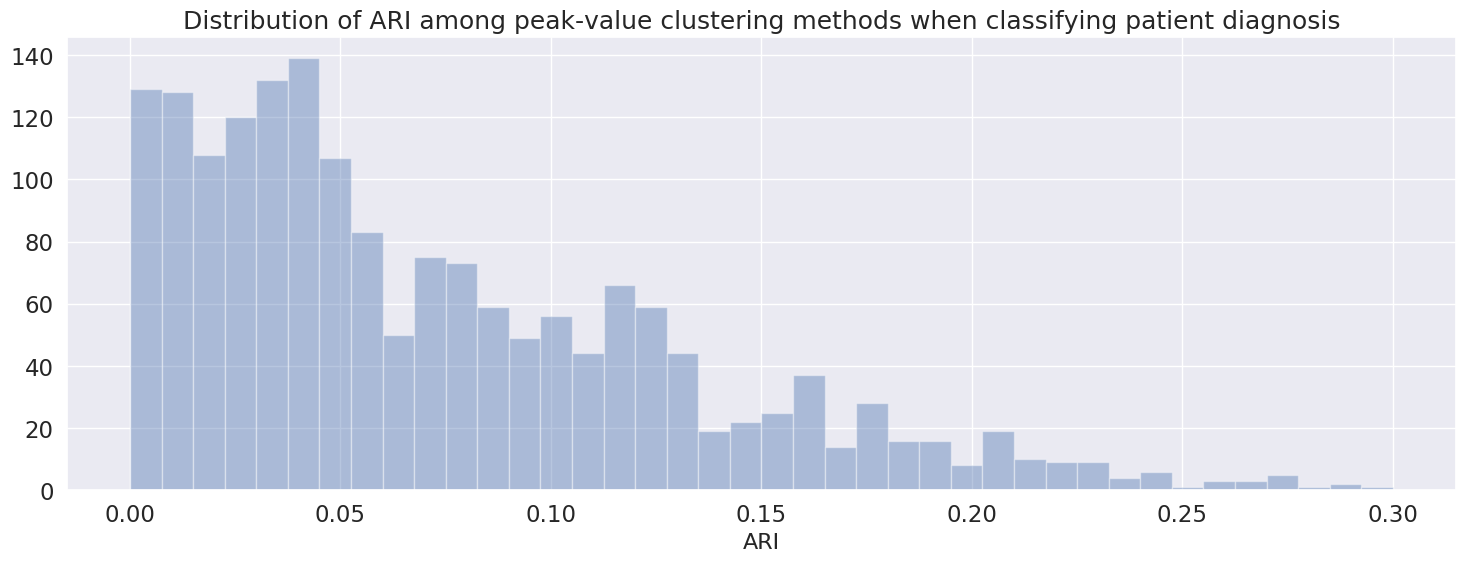
\includegraphics[width=\textwidth]{results/tsc-ind-ari.png}
    %% Creator: Matplotlib, PGF backend
%%
%% To include the figure in your LaTeX document, write
%%   \input{<filename>.pgf}
%%
%% Make sure the required packages are loaded in your preamble
%%   \usepackage{pgf}
%%
%% Figures using additional raster images can only be included by \input if
%% they are in the same directory as the main LaTeX file. For loading figures
%% from other directories you can use the `import` package
%%   \usepackage{import}
%% and then include the figures with
%%   \import{<path to file>}{<filename>.pgf}
%%
%% Matplotlib used the following preamble
%%
\begingroup%
\makeatletter%
\begin{pgfpicture}%
\pgfpathrectangle{\pgfpointorigin}{\pgfqpoint{6.340000in}{2.340000in}}%
\pgfusepath{use as bounding box, clip}%
\begin{pgfscope}%
\pgfsetbuttcap%
\pgfsetmiterjoin%
\definecolor{currentfill}{rgb}{1.000000,1.000000,1.000000}%
\pgfsetfillcolor{currentfill}%
\pgfsetlinewidth{0.000000pt}%
\definecolor{currentstroke}{rgb}{1.000000,1.000000,1.000000}%
\pgfsetstrokecolor{currentstroke}%
\pgfsetdash{}{0pt}%
\pgfpathmoveto{\pgfqpoint{0.000000in}{-0.000000in}}%
\pgfpathlineto{\pgfqpoint{6.340000in}{-0.000000in}}%
\pgfpathlineto{\pgfqpoint{6.340000in}{2.340000in}}%
\pgfpathlineto{\pgfqpoint{0.000000in}{2.340000in}}%
\pgfpathclose%
\pgfusepath{fill}%
\end{pgfscope}%
\begin{pgfscope}%
\pgfsetbuttcap%
\pgfsetmiterjoin%
\definecolor{currentfill}{rgb}{0.917647,0.917647,0.949020}%
\pgfsetfillcolor{currentfill}%
\pgfsetlinewidth{0.000000pt}%
\definecolor{currentstroke}{rgb}{0.000000,0.000000,0.000000}%
\pgfsetstrokecolor{currentstroke}%
\pgfsetstrokeopacity{0.000000}%
\pgfsetdash{}{0pt}%
\pgfpathmoveto{\pgfqpoint{0.650810in}{0.557870in}}%
\pgfpathlineto{\pgfqpoint{6.240000in}{0.557870in}}%
\pgfpathlineto{\pgfqpoint{6.240000in}{2.240000in}}%
\pgfpathlineto{\pgfqpoint{0.650810in}{2.240000in}}%
\pgfpathclose%
\pgfusepath{fill}%
\end{pgfscope}%
\begin{pgfscope}%
\pgfpathrectangle{\pgfqpoint{0.650810in}{0.557870in}}{\pgfqpoint{5.589190in}{1.682130in}}%
\pgfusepath{clip}%
\pgfsetroundcap%
\pgfsetroundjoin%
\pgfsetlinewidth{1.003750pt}%
\definecolor{currentstroke}{rgb}{1.000000,1.000000,1.000000}%
\pgfsetstrokecolor{currentstroke}%
\pgfsetdash{}{0pt}%
\pgfpathmoveto{\pgfqpoint{1.025210in}{0.557870in}}%
\pgfpathlineto{\pgfqpoint{1.025210in}{2.240000in}}%
\pgfusepath{stroke}%
\end{pgfscope}%
\begin{pgfscope}%
\definecolor{textcolor}{rgb}{0.150000,0.150000,0.150000}%
\pgfsetstrokecolor{textcolor}%
\pgfsetfillcolor{textcolor}%
\pgftext[x=1.025210in,y=0.425926in,,top]{\color{textcolor}\sffamily\fontsize{11.000000}{13.200000}\selectfont \(\displaystyle -0.1\)}%
\end{pgfscope}%
\begin{pgfscope}%
\pgfpathrectangle{\pgfqpoint{0.650810in}{0.557870in}}{\pgfqpoint{5.589190in}{1.682130in}}%
\pgfusepath{clip}%
\pgfsetroundcap%
\pgfsetroundjoin%
\pgfsetlinewidth{1.003750pt}%
\definecolor{currentstroke}{rgb}{1.000000,1.000000,1.000000}%
\pgfsetstrokecolor{currentstroke}%
\pgfsetdash{}{0pt}%
\pgfpathmoveto{\pgfqpoint{2.135005in}{0.557870in}}%
\pgfpathlineto{\pgfqpoint{2.135005in}{2.240000in}}%
\pgfusepath{stroke}%
\end{pgfscope}%
\begin{pgfscope}%
\definecolor{textcolor}{rgb}{0.150000,0.150000,0.150000}%
\pgfsetstrokecolor{textcolor}%
\pgfsetfillcolor{textcolor}%
\pgftext[x=2.135005in,y=0.425926in,,top]{\color{textcolor}\sffamily\fontsize{11.000000}{13.200000}\selectfont \(\displaystyle 0.0\)}%
\end{pgfscope}%
\begin{pgfscope}%
\pgfpathrectangle{\pgfqpoint{0.650810in}{0.557870in}}{\pgfqpoint{5.589190in}{1.682130in}}%
\pgfusepath{clip}%
\pgfsetroundcap%
\pgfsetroundjoin%
\pgfsetlinewidth{1.003750pt}%
\definecolor{currentstroke}{rgb}{1.000000,1.000000,1.000000}%
\pgfsetstrokecolor{currentstroke}%
\pgfsetdash{}{0pt}%
\pgfpathmoveto{\pgfqpoint{3.244800in}{0.557870in}}%
\pgfpathlineto{\pgfqpoint{3.244800in}{2.240000in}}%
\pgfusepath{stroke}%
\end{pgfscope}%
\begin{pgfscope}%
\definecolor{textcolor}{rgb}{0.150000,0.150000,0.150000}%
\pgfsetstrokecolor{textcolor}%
\pgfsetfillcolor{textcolor}%
\pgftext[x=3.244800in,y=0.425926in,,top]{\color{textcolor}\sffamily\fontsize{11.000000}{13.200000}\selectfont \(\displaystyle 0.1\)}%
\end{pgfscope}%
\begin{pgfscope}%
\pgfpathrectangle{\pgfqpoint{0.650810in}{0.557870in}}{\pgfqpoint{5.589190in}{1.682130in}}%
\pgfusepath{clip}%
\pgfsetroundcap%
\pgfsetroundjoin%
\pgfsetlinewidth{1.003750pt}%
\definecolor{currentstroke}{rgb}{1.000000,1.000000,1.000000}%
\pgfsetstrokecolor{currentstroke}%
\pgfsetdash{}{0pt}%
\pgfpathmoveto{\pgfqpoint{4.354596in}{0.557870in}}%
\pgfpathlineto{\pgfqpoint{4.354596in}{2.240000in}}%
\pgfusepath{stroke}%
\end{pgfscope}%
\begin{pgfscope}%
\definecolor{textcolor}{rgb}{0.150000,0.150000,0.150000}%
\pgfsetstrokecolor{textcolor}%
\pgfsetfillcolor{textcolor}%
\pgftext[x=4.354596in,y=0.425926in,,top]{\color{textcolor}\sffamily\fontsize{11.000000}{13.200000}\selectfont \(\displaystyle 0.2\)}%
\end{pgfscope}%
\begin{pgfscope}%
\pgfpathrectangle{\pgfqpoint{0.650810in}{0.557870in}}{\pgfqpoint{5.589190in}{1.682130in}}%
\pgfusepath{clip}%
\pgfsetroundcap%
\pgfsetroundjoin%
\pgfsetlinewidth{1.003750pt}%
\definecolor{currentstroke}{rgb}{1.000000,1.000000,1.000000}%
\pgfsetstrokecolor{currentstroke}%
\pgfsetdash{}{0pt}%
\pgfpathmoveto{\pgfqpoint{5.464391in}{0.557870in}}%
\pgfpathlineto{\pgfqpoint{5.464391in}{2.240000in}}%
\pgfusepath{stroke}%
\end{pgfscope}%
\begin{pgfscope}%
\definecolor{textcolor}{rgb}{0.150000,0.150000,0.150000}%
\pgfsetstrokecolor{textcolor}%
\pgfsetfillcolor{textcolor}%
\pgftext[x=5.464391in,y=0.425926in,,top]{\color{textcolor}\sffamily\fontsize{11.000000}{13.200000}\selectfont \(\displaystyle 0.3\)}%
\end{pgfscope}%
\begin{pgfscope}%
\definecolor{textcolor}{rgb}{0.150000,0.150000,0.150000}%
\pgfsetstrokecolor{textcolor}%
\pgfsetfillcolor{textcolor}%
\pgftext[x=3.445405in,y=0.235185in,,top]{\color{textcolor}\sffamily\fontsize{11.000000}{13.200000}\selectfont ARI}%
\end{pgfscope}%
\begin{pgfscope}%
\pgfpathrectangle{\pgfqpoint{0.650810in}{0.557870in}}{\pgfqpoint{5.589190in}{1.682130in}}%
\pgfusepath{clip}%
\pgfsetroundcap%
\pgfsetroundjoin%
\pgfsetlinewidth{1.003750pt}%
\definecolor{currentstroke}{rgb}{1.000000,1.000000,1.000000}%
\pgfsetstrokecolor{currentstroke}%
\pgfsetdash{}{0pt}%
\pgfpathmoveto{\pgfqpoint{0.650810in}{0.557870in}}%
\pgfpathlineto{\pgfqpoint{6.240000in}{0.557870in}}%
\pgfusepath{stroke}%
\end{pgfscope}%
\begin{pgfscope}%
\definecolor{textcolor}{rgb}{0.150000,0.150000,0.150000}%
\pgfsetstrokecolor{textcolor}%
\pgfsetfillcolor{textcolor}%
\pgftext[x=0.442824in,y=0.505064in,left,base]{\color{textcolor}\sffamily\fontsize{11.000000}{13.200000}\selectfont \(\displaystyle 0\)}%
\end{pgfscope}%
\begin{pgfscope}%
\pgfpathrectangle{\pgfqpoint{0.650810in}{0.557870in}}{\pgfqpoint{5.589190in}{1.682130in}}%
\pgfusepath{clip}%
\pgfsetroundcap%
\pgfsetroundjoin%
\pgfsetlinewidth{1.003750pt}%
\definecolor{currentstroke}{rgb}{1.000000,1.000000,1.000000}%
\pgfsetstrokecolor{currentstroke}%
\pgfsetdash{}{0pt}%
\pgfpathmoveto{\pgfqpoint{0.650810in}{1.006618in}}%
\pgfpathlineto{\pgfqpoint{6.240000in}{1.006618in}}%
\pgfusepath{stroke}%
\end{pgfscope}%
\begin{pgfscope}%
\definecolor{textcolor}{rgb}{0.150000,0.150000,0.150000}%
\pgfsetstrokecolor{textcolor}%
\pgfsetfillcolor{textcolor}%
\pgftext[x=0.290741in,y=0.953811in,left,base]{\color{textcolor}\sffamily\fontsize{11.000000}{13.200000}\selectfont \(\displaystyle 100\)}%
\end{pgfscope}%
\begin{pgfscope}%
\pgfpathrectangle{\pgfqpoint{0.650810in}{0.557870in}}{\pgfqpoint{5.589190in}{1.682130in}}%
\pgfusepath{clip}%
\pgfsetroundcap%
\pgfsetroundjoin%
\pgfsetlinewidth{1.003750pt}%
\definecolor{currentstroke}{rgb}{1.000000,1.000000,1.000000}%
\pgfsetstrokecolor{currentstroke}%
\pgfsetdash{}{0pt}%
\pgfpathmoveto{\pgfqpoint{0.650810in}{1.455365in}}%
\pgfpathlineto{\pgfqpoint{6.240000in}{1.455365in}}%
\pgfusepath{stroke}%
\end{pgfscope}%
\begin{pgfscope}%
\definecolor{textcolor}{rgb}{0.150000,0.150000,0.150000}%
\pgfsetstrokecolor{textcolor}%
\pgfsetfillcolor{textcolor}%
\pgftext[x=0.290741in,y=1.402558in,left,base]{\color{textcolor}\sffamily\fontsize{11.000000}{13.200000}\selectfont \(\displaystyle 200\)}%
\end{pgfscope}%
\begin{pgfscope}%
\pgfpathrectangle{\pgfqpoint{0.650810in}{0.557870in}}{\pgfqpoint{5.589190in}{1.682130in}}%
\pgfusepath{clip}%
\pgfsetroundcap%
\pgfsetroundjoin%
\pgfsetlinewidth{1.003750pt}%
\definecolor{currentstroke}{rgb}{1.000000,1.000000,1.000000}%
\pgfsetstrokecolor{currentstroke}%
\pgfsetdash{}{0pt}%
\pgfpathmoveto{\pgfqpoint{0.650810in}{1.904113in}}%
\pgfpathlineto{\pgfqpoint{6.240000in}{1.904113in}}%
\pgfusepath{stroke}%
\end{pgfscope}%
\begin{pgfscope}%
\definecolor{textcolor}{rgb}{0.150000,0.150000,0.150000}%
\pgfsetstrokecolor{textcolor}%
\pgfsetfillcolor{textcolor}%
\pgftext[x=0.290741in,y=1.851306in,left,base]{\color{textcolor}\sffamily\fontsize{11.000000}{13.200000}\selectfont \(\displaystyle 300\)}%
\end{pgfscope}%
\begin{pgfscope}%
\definecolor{textcolor}{rgb}{0.150000,0.150000,0.150000}%
\pgfsetstrokecolor{textcolor}%
\pgfsetfillcolor{textcolor}%
\pgftext[x=0.235185in,y=1.398935in,,bottom,rotate=90.000000]{\color{textcolor}\sffamily\fontsize{11.000000}{13.200000}\selectfont Occurance}%
\end{pgfscope}%
\begin{pgfscope}%
\pgfpathrectangle{\pgfqpoint{0.650810in}{0.557870in}}{\pgfqpoint{5.589190in}{1.682130in}}%
\pgfusepath{clip}%
\pgfsetbuttcap%
\pgfsetmiterjoin%
\definecolor{currentfill}{rgb}{0.298039,0.447059,0.690196}%
\pgfsetfillcolor{currentfill}%
\pgfsetfillopacity{0.400000}%
\pgfsetlinewidth{1.003750pt}%
\definecolor{currentstroke}{rgb}{1.000000,1.000000,1.000000}%
\pgfsetstrokecolor{currentstroke}%
\pgfsetstrokeopacity{0.400000}%
\pgfsetdash{}{0pt}%
\pgfpathmoveto{\pgfqpoint{0.904864in}{0.557870in}}%
\pgfpathlineto{\pgfqpoint{1.050038in}{0.557870in}}%
\pgfpathlineto{\pgfqpoint{1.050038in}{0.580308in}}%
\pgfpathlineto{\pgfqpoint{0.904864in}{0.580308in}}%
\pgfpathclose%
\pgfusepath{stroke,fill}%
\end{pgfscope}%
\begin{pgfscope}%
\pgfpathrectangle{\pgfqpoint{0.650810in}{0.557870in}}{\pgfqpoint{5.589190in}{1.682130in}}%
\pgfusepath{clip}%
\pgfsetbuttcap%
\pgfsetmiterjoin%
\definecolor{currentfill}{rgb}{0.298039,0.447059,0.690196}%
\pgfsetfillcolor{currentfill}%
\pgfsetfillopacity{0.400000}%
\pgfsetlinewidth{1.003750pt}%
\definecolor{currentstroke}{rgb}{1.000000,1.000000,1.000000}%
\pgfsetstrokecolor{currentstroke}%
\pgfsetstrokeopacity{0.400000}%
\pgfsetdash{}{0pt}%
\pgfpathmoveto{\pgfqpoint{1.050038in}{0.557870in}}%
\pgfpathlineto{\pgfqpoint{1.195212in}{0.557870in}}%
\pgfpathlineto{\pgfqpoint{1.195212in}{0.602745in}}%
\pgfpathlineto{\pgfqpoint{1.050038in}{0.602745in}}%
\pgfpathclose%
\pgfusepath{stroke,fill}%
\end{pgfscope}%
\begin{pgfscope}%
\pgfpathrectangle{\pgfqpoint{0.650810in}{0.557870in}}{\pgfqpoint{5.589190in}{1.682130in}}%
\pgfusepath{clip}%
\pgfsetbuttcap%
\pgfsetmiterjoin%
\definecolor{currentfill}{rgb}{0.298039,0.447059,0.690196}%
\pgfsetfillcolor{currentfill}%
\pgfsetfillopacity{0.400000}%
\pgfsetlinewidth{1.003750pt}%
\definecolor{currentstroke}{rgb}{1.000000,1.000000,1.000000}%
\pgfsetstrokecolor{currentstroke}%
\pgfsetstrokeopacity{0.400000}%
\pgfsetdash{}{0pt}%
\pgfpathmoveto{\pgfqpoint{1.195212in}{0.557870in}}%
\pgfpathlineto{\pgfqpoint{1.340386in}{0.557870in}}%
\pgfpathlineto{\pgfqpoint{1.340386in}{0.670057in}}%
\pgfpathlineto{\pgfqpoint{1.195212in}{0.670057in}}%
\pgfpathclose%
\pgfusepath{stroke,fill}%
\end{pgfscope}%
\begin{pgfscope}%
\pgfpathrectangle{\pgfqpoint{0.650810in}{0.557870in}}{\pgfqpoint{5.589190in}{1.682130in}}%
\pgfusepath{clip}%
\pgfsetbuttcap%
\pgfsetmiterjoin%
\definecolor{currentfill}{rgb}{0.298039,0.447059,0.690196}%
\pgfsetfillcolor{currentfill}%
\pgfsetfillopacity{0.400000}%
\pgfsetlinewidth{1.003750pt}%
\definecolor{currentstroke}{rgb}{1.000000,1.000000,1.000000}%
\pgfsetstrokecolor{currentstroke}%
\pgfsetstrokeopacity{0.400000}%
\pgfsetdash{}{0pt}%
\pgfpathmoveto{\pgfqpoint{1.340386in}{0.557870in}}%
\pgfpathlineto{\pgfqpoint{1.485560in}{0.557870in}}%
\pgfpathlineto{\pgfqpoint{1.485560in}{0.692495in}}%
\pgfpathlineto{\pgfqpoint{1.340386in}{0.692495in}}%
\pgfpathclose%
\pgfusepath{stroke,fill}%
\end{pgfscope}%
\begin{pgfscope}%
\pgfpathrectangle{\pgfqpoint{0.650810in}{0.557870in}}{\pgfqpoint{5.589190in}{1.682130in}}%
\pgfusepath{clip}%
\pgfsetbuttcap%
\pgfsetmiterjoin%
\definecolor{currentfill}{rgb}{0.298039,0.447059,0.690196}%
\pgfsetfillcolor{currentfill}%
\pgfsetfillopacity{0.400000}%
\pgfsetlinewidth{1.003750pt}%
\definecolor{currentstroke}{rgb}{1.000000,1.000000,1.000000}%
\pgfsetstrokecolor{currentstroke}%
\pgfsetstrokeopacity{0.400000}%
\pgfsetdash{}{0pt}%
\pgfpathmoveto{\pgfqpoint{1.485560in}{0.557870in}}%
\pgfpathlineto{\pgfqpoint{1.630733in}{0.557870in}}%
\pgfpathlineto{\pgfqpoint{1.630733in}{0.782244in}}%
\pgfpathlineto{\pgfqpoint{1.485560in}{0.782244in}}%
\pgfpathclose%
\pgfusepath{stroke,fill}%
\end{pgfscope}%
\begin{pgfscope}%
\pgfpathrectangle{\pgfqpoint{0.650810in}{0.557870in}}{\pgfqpoint{5.589190in}{1.682130in}}%
\pgfusepath{clip}%
\pgfsetbuttcap%
\pgfsetmiterjoin%
\definecolor{currentfill}{rgb}{0.298039,0.447059,0.690196}%
\pgfsetfillcolor{currentfill}%
\pgfsetfillopacity{0.400000}%
\pgfsetlinewidth{1.003750pt}%
\definecolor{currentstroke}{rgb}{1.000000,1.000000,1.000000}%
\pgfsetstrokecolor{currentstroke}%
\pgfsetstrokeopacity{0.400000}%
\pgfsetdash{}{0pt}%
\pgfpathmoveto{\pgfqpoint{1.630733in}{0.557870in}}%
\pgfpathlineto{\pgfqpoint{1.775907in}{0.557870in}}%
\pgfpathlineto{\pgfqpoint{1.775907in}{0.889943in}}%
\pgfpathlineto{\pgfqpoint{1.630733in}{0.889943in}}%
\pgfpathclose%
\pgfusepath{stroke,fill}%
\end{pgfscope}%
\begin{pgfscope}%
\pgfpathrectangle{\pgfqpoint{0.650810in}{0.557870in}}{\pgfqpoint{5.589190in}{1.682130in}}%
\pgfusepath{clip}%
\pgfsetbuttcap%
\pgfsetmiterjoin%
\definecolor{currentfill}{rgb}{0.298039,0.447059,0.690196}%
\pgfsetfillcolor{currentfill}%
\pgfsetfillopacity{0.400000}%
\pgfsetlinewidth{1.003750pt}%
\definecolor{currentstroke}{rgb}{1.000000,1.000000,1.000000}%
\pgfsetstrokecolor{currentstroke}%
\pgfsetstrokeopacity{0.400000}%
\pgfsetdash{}{0pt}%
\pgfpathmoveto{\pgfqpoint{1.775907in}{0.557870in}}%
\pgfpathlineto{\pgfqpoint{1.921081in}{0.557870in}}%
\pgfpathlineto{\pgfqpoint{1.921081in}{1.181629in}}%
\pgfpathlineto{\pgfqpoint{1.775907in}{1.181629in}}%
\pgfpathclose%
\pgfusepath{stroke,fill}%
\end{pgfscope}%
\begin{pgfscope}%
\pgfpathrectangle{\pgfqpoint{0.650810in}{0.557870in}}{\pgfqpoint{5.589190in}{1.682130in}}%
\pgfusepath{clip}%
\pgfsetbuttcap%
\pgfsetmiterjoin%
\definecolor{currentfill}{rgb}{0.298039,0.447059,0.690196}%
\pgfsetfillcolor{currentfill}%
\pgfsetfillopacity{0.400000}%
\pgfsetlinewidth{1.003750pt}%
\definecolor{currentstroke}{rgb}{1.000000,1.000000,1.000000}%
\pgfsetstrokecolor{currentstroke}%
\pgfsetstrokeopacity{0.400000}%
\pgfsetdash{}{0pt}%
\pgfpathmoveto{\pgfqpoint{1.921081in}{0.557870in}}%
\pgfpathlineto{\pgfqpoint{2.066255in}{0.557870in}}%
\pgfpathlineto{\pgfqpoint{2.066255in}{2.159899in}}%
\pgfpathlineto{\pgfqpoint{1.921081in}{2.159899in}}%
\pgfpathclose%
\pgfusepath{stroke,fill}%
\end{pgfscope}%
\begin{pgfscope}%
\pgfpathrectangle{\pgfqpoint{0.650810in}{0.557870in}}{\pgfqpoint{5.589190in}{1.682130in}}%
\pgfusepath{clip}%
\pgfsetbuttcap%
\pgfsetmiterjoin%
\definecolor{currentfill}{rgb}{0.298039,0.447059,0.690196}%
\pgfsetfillcolor{currentfill}%
\pgfsetfillopacity{0.400000}%
\pgfsetlinewidth{1.003750pt}%
\definecolor{currentstroke}{rgb}{1.000000,1.000000,1.000000}%
\pgfsetstrokecolor{currentstroke}%
\pgfsetstrokeopacity{0.400000}%
\pgfsetdash{}{0pt}%
\pgfpathmoveto{\pgfqpoint{2.066255in}{0.557870in}}%
\pgfpathlineto{\pgfqpoint{2.211428in}{0.557870in}}%
\pgfpathlineto{\pgfqpoint{2.211428in}{1.500240in}}%
\pgfpathlineto{\pgfqpoint{2.066255in}{1.500240in}}%
\pgfpathclose%
\pgfusepath{stroke,fill}%
\end{pgfscope}%
\begin{pgfscope}%
\pgfpathrectangle{\pgfqpoint{0.650810in}{0.557870in}}{\pgfqpoint{5.589190in}{1.682130in}}%
\pgfusepath{clip}%
\pgfsetbuttcap%
\pgfsetmiterjoin%
\definecolor{currentfill}{rgb}{0.298039,0.447059,0.690196}%
\pgfsetfillcolor{currentfill}%
\pgfsetfillopacity{0.400000}%
\pgfsetlinewidth{1.003750pt}%
\definecolor{currentstroke}{rgb}{1.000000,1.000000,1.000000}%
\pgfsetstrokecolor{currentstroke}%
\pgfsetstrokeopacity{0.400000}%
\pgfsetdash{}{0pt}%
\pgfpathmoveto{\pgfqpoint{2.211428in}{0.557870in}}%
\pgfpathlineto{\pgfqpoint{2.356602in}{0.557870in}}%
\pgfpathlineto{\pgfqpoint{2.356602in}{1.540627in}}%
\pgfpathlineto{\pgfqpoint{2.211428in}{1.540627in}}%
\pgfpathclose%
\pgfusepath{stroke,fill}%
\end{pgfscope}%
\begin{pgfscope}%
\pgfpathrectangle{\pgfqpoint{0.650810in}{0.557870in}}{\pgfqpoint{5.589190in}{1.682130in}}%
\pgfusepath{clip}%
\pgfsetbuttcap%
\pgfsetmiterjoin%
\definecolor{currentfill}{rgb}{0.298039,0.447059,0.690196}%
\pgfsetfillcolor{currentfill}%
\pgfsetfillopacity{0.400000}%
\pgfsetlinewidth{1.003750pt}%
\definecolor{currentstroke}{rgb}{1.000000,1.000000,1.000000}%
\pgfsetstrokecolor{currentstroke}%
\pgfsetstrokeopacity{0.400000}%
\pgfsetdash{}{0pt}%
\pgfpathmoveto{\pgfqpoint{2.356602in}{0.557870in}}%
\pgfpathlineto{\pgfqpoint{2.501776in}{0.557870in}}%
\pgfpathlineto{\pgfqpoint{2.501776in}{1.576527in}}%
\pgfpathlineto{\pgfqpoint{2.356602in}{1.576527in}}%
\pgfpathclose%
\pgfusepath{stroke,fill}%
\end{pgfscope}%
\begin{pgfscope}%
\pgfpathrectangle{\pgfqpoint{0.650810in}{0.557870in}}{\pgfqpoint{5.589190in}{1.682130in}}%
\pgfusepath{clip}%
\pgfsetbuttcap%
\pgfsetmiterjoin%
\definecolor{currentfill}{rgb}{0.298039,0.447059,0.690196}%
\pgfsetfillcolor{currentfill}%
\pgfsetfillopacity{0.400000}%
\pgfsetlinewidth{1.003750pt}%
\definecolor{currentstroke}{rgb}{1.000000,1.000000,1.000000}%
\pgfsetstrokecolor{currentstroke}%
\pgfsetstrokeopacity{0.400000}%
\pgfsetdash{}{0pt}%
\pgfpathmoveto{\pgfqpoint{2.501776in}{0.557870in}}%
\pgfpathlineto{\pgfqpoint{2.646950in}{0.557870in}}%
\pgfpathlineto{\pgfqpoint{2.646950in}{1.500240in}}%
\pgfpathlineto{\pgfqpoint{2.501776in}{1.500240in}}%
\pgfpathclose%
\pgfusepath{stroke,fill}%
\end{pgfscope}%
\begin{pgfscope}%
\pgfpathrectangle{\pgfqpoint{0.650810in}{0.557870in}}{\pgfqpoint{5.589190in}{1.682130in}}%
\pgfusepath{clip}%
\pgfsetbuttcap%
\pgfsetmiterjoin%
\definecolor{currentfill}{rgb}{0.298039,0.447059,0.690196}%
\pgfsetfillcolor{currentfill}%
\pgfsetfillopacity{0.400000}%
\pgfsetlinewidth{1.003750pt}%
\definecolor{currentstroke}{rgb}{1.000000,1.000000,1.000000}%
\pgfsetstrokecolor{currentstroke}%
\pgfsetstrokeopacity{0.400000}%
\pgfsetdash{}{0pt}%
\pgfpathmoveto{\pgfqpoint{2.646950in}{0.557870in}}%
\pgfpathlineto{\pgfqpoint{2.792123in}{0.557870in}}%
\pgfpathlineto{\pgfqpoint{2.792123in}{1.338691in}}%
\pgfpathlineto{\pgfqpoint{2.646950in}{1.338691in}}%
\pgfpathclose%
\pgfusepath{stroke,fill}%
\end{pgfscope}%
\begin{pgfscope}%
\pgfpathrectangle{\pgfqpoint{0.650810in}{0.557870in}}{\pgfqpoint{5.589190in}{1.682130in}}%
\pgfusepath{clip}%
\pgfsetbuttcap%
\pgfsetmiterjoin%
\definecolor{currentfill}{rgb}{0.298039,0.447059,0.690196}%
\pgfsetfillcolor{currentfill}%
\pgfsetfillopacity{0.400000}%
\pgfsetlinewidth{1.003750pt}%
\definecolor{currentstroke}{rgb}{1.000000,1.000000,1.000000}%
\pgfsetstrokecolor{currentstroke}%
\pgfsetstrokeopacity{0.400000}%
\pgfsetdash{}{0pt}%
\pgfpathmoveto{\pgfqpoint{2.792123in}{0.557870in}}%
\pgfpathlineto{\pgfqpoint{2.937297in}{0.557870in}}%
\pgfpathlineto{\pgfqpoint{2.937297in}{0.984180in}}%
\pgfpathlineto{\pgfqpoint{2.792123in}{0.984180in}}%
\pgfpathclose%
\pgfusepath{stroke,fill}%
\end{pgfscope}%
\begin{pgfscope}%
\pgfpathrectangle{\pgfqpoint{0.650810in}{0.557870in}}{\pgfqpoint{5.589190in}{1.682130in}}%
\pgfusepath{clip}%
\pgfsetbuttcap%
\pgfsetmiterjoin%
\definecolor{currentfill}{rgb}{0.298039,0.447059,0.690196}%
\pgfsetfillcolor{currentfill}%
\pgfsetfillopacity{0.400000}%
\pgfsetlinewidth{1.003750pt}%
\definecolor{currentstroke}{rgb}{1.000000,1.000000,1.000000}%
\pgfsetstrokecolor{currentstroke}%
\pgfsetstrokeopacity{0.400000}%
\pgfsetdash{}{0pt}%
\pgfpathmoveto{\pgfqpoint{2.937297in}{0.557870in}}%
\pgfpathlineto{\pgfqpoint{3.082471in}{0.557870in}}%
\pgfpathlineto{\pgfqpoint{3.082471in}{1.132267in}}%
\pgfpathlineto{\pgfqpoint{2.937297in}{1.132267in}}%
\pgfpathclose%
\pgfusepath{stroke,fill}%
\end{pgfscope}%
\begin{pgfscope}%
\pgfpathrectangle{\pgfqpoint{0.650810in}{0.557870in}}{\pgfqpoint{5.589190in}{1.682130in}}%
\pgfusepath{clip}%
\pgfsetbuttcap%
\pgfsetmiterjoin%
\definecolor{currentfill}{rgb}{0.298039,0.447059,0.690196}%
\pgfsetfillcolor{currentfill}%
\pgfsetfillopacity{0.400000}%
\pgfsetlinewidth{1.003750pt}%
\definecolor{currentstroke}{rgb}{1.000000,1.000000,1.000000}%
\pgfsetstrokecolor{currentstroke}%
\pgfsetstrokeopacity{0.400000}%
\pgfsetdash{}{0pt}%
\pgfpathmoveto{\pgfqpoint{3.082471in}{0.557870in}}%
\pgfpathlineto{\pgfqpoint{3.227645in}{0.557870in}}%
\pgfpathlineto{\pgfqpoint{3.227645in}{0.975205in}}%
\pgfpathlineto{\pgfqpoint{3.082471in}{0.975205in}}%
\pgfpathclose%
\pgfusepath{stroke,fill}%
\end{pgfscope}%
\begin{pgfscope}%
\pgfpathrectangle{\pgfqpoint{0.650810in}{0.557870in}}{\pgfqpoint{5.589190in}{1.682130in}}%
\pgfusepath{clip}%
\pgfsetbuttcap%
\pgfsetmiterjoin%
\definecolor{currentfill}{rgb}{0.298039,0.447059,0.690196}%
\pgfsetfillcolor{currentfill}%
\pgfsetfillopacity{0.400000}%
\pgfsetlinewidth{1.003750pt}%
\definecolor{currentstroke}{rgb}{1.000000,1.000000,1.000000}%
\pgfsetstrokecolor{currentstroke}%
\pgfsetstrokeopacity{0.400000}%
\pgfsetdash{}{0pt}%
\pgfpathmoveto{\pgfqpoint{3.227645in}{0.557870in}}%
\pgfpathlineto{\pgfqpoint{3.372818in}{0.557870in}}%
\pgfpathlineto{\pgfqpoint{3.372818in}{0.948281in}}%
\pgfpathlineto{\pgfqpoint{3.227645in}{0.948281in}}%
\pgfpathclose%
\pgfusepath{stroke,fill}%
\end{pgfscope}%
\begin{pgfscope}%
\pgfpathrectangle{\pgfqpoint{0.650810in}{0.557870in}}{\pgfqpoint{5.589190in}{1.682130in}}%
\pgfusepath{clip}%
\pgfsetbuttcap%
\pgfsetmiterjoin%
\definecolor{currentfill}{rgb}{0.298039,0.447059,0.690196}%
\pgfsetfillcolor{currentfill}%
\pgfsetfillopacity{0.400000}%
\pgfsetlinewidth{1.003750pt}%
\definecolor{currentstroke}{rgb}{1.000000,1.000000,1.000000}%
\pgfsetstrokecolor{currentstroke}%
\pgfsetstrokeopacity{0.400000}%
\pgfsetdash{}{0pt}%
\pgfpathmoveto{\pgfqpoint{3.372818in}{0.557870in}}%
\pgfpathlineto{\pgfqpoint{3.517992in}{0.557870in}}%
\pgfpathlineto{\pgfqpoint{3.517992in}{1.073930in}}%
\pgfpathlineto{\pgfqpoint{3.372818in}{1.073930in}}%
\pgfpathclose%
\pgfusepath{stroke,fill}%
\end{pgfscope}%
\begin{pgfscope}%
\pgfpathrectangle{\pgfqpoint{0.650810in}{0.557870in}}{\pgfqpoint{5.589190in}{1.682130in}}%
\pgfusepath{clip}%
\pgfsetbuttcap%
\pgfsetmiterjoin%
\definecolor{currentfill}{rgb}{0.298039,0.447059,0.690196}%
\pgfsetfillcolor{currentfill}%
\pgfsetfillopacity{0.400000}%
\pgfsetlinewidth{1.003750pt}%
\definecolor{currentstroke}{rgb}{1.000000,1.000000,1.000000}%
\pgfsetstrokecolor{currentstroke}%
\pgfsetstrokeopacity{0.400000}%
\pgfsetdash{}{0pt}%
\pgfpathmoveto{\pgfqpoint{3.517992in}{0.557870in}}%
\pgfpathlineto{\pgfqpoint{3.663166in}{0.557870in}}%
\pgfpathlineto{\pgfqpoint{3.663166in}{0.849556in}}%
\pgfpathlineto{\pgfqpoint{3.517992in}{0.849556in}}%
\pgfpathclose%
\pgfusepath{stroke,fill}%
\end{pgfscope}%
\begin{pgfscope}%
\pgfpathrectangle{\pgfqpoint{0.650810in}{0.557870in}}{\pgfqpoint{5.589190in}{1.682130in}}%
\pgfusepath{clip}%
\pgfsetbuttcap%
\pgfsetmiterjoin%
\definecolor{currentfill}{rgb}{0.298039,0.447059,0.690196}%
\pgfsetfillcolor{currentfill}%
\pgfsetfillopacity{0.400000}%
\pgfsetlinewidth{1.003750pt}%
\definecolor{currentstroke}{rgb}{1.000000,1.000000,1.000000}%
\pgfsetstrokecolor{currentstroke}%
\pgfsetstrokeopacity{0.400000}%
\pgfsetdash{}{0pt}%
\pgfpathmoveto{\pgfqpoint{3.663166in}{0.557870in}}%
\pgfpathlineto{\pgfqpoint{3.808340in}{0.557870in}}%
\pgfpathlineto{\pgfqpoint{3.808340in}{0.737369in}}%
\pgfpathlineto{\pgfqpoint{3.663166in}{0.737369in}}%
\pgfpathclose%
\pgfusepath{stroke,fill}%
\end{pgfscope}%
\begin{pgfscope}%
\pgfpathrectangle{\pgfqpoint{0.650810in}{0.557870in}}{\pgfqpoint{5.589190in}{1.682130in}}%
\pgfusepath{clip}%
\pgfsetbuttcap%
\pgfsetmiterjoin%
\definecolor{currentfill}{rgb}{0.298039,0.447059,0.690196}%
\pgfsetfillcolor{currentfill}%
\pgfsetfillopacity{0.400000}%
\pgfsetlinewidth{1.003750pt}%
\definecolor{currentstroke}{rgb}{1.000000,1.000000,1.000000}%
\pgfsetstrokecolor{currentstroke}%
\pgfsetstrokeopacity{0.400000}%
\pgfsetdash{}{0pt}%
\pgfpathmoveto{\pgfqpoint{3.808340in}{0.557870in}}%
\pgfpathlineto{\pgfqpoint{3.953513in}{0.557870in}}%
\pgfpathlineto{\pgfqpoint{3.953513in}{0.746344in}}%
\pgfpathlineto{\pgfqpoint{3.808340in}{0.746344in}}%
\pgfpathclose%
\pgfusepath{stroke,fill}%
\end{pgfscope}%
\begin{pgfscope}%
\pgfpathrectangle{\pgfqpoint{0.650810in}{0.557870in}}{\pgfqpoint{5.589190in}{1.682130in}}%
\pgfusepath{clip}%
\pgfsetbuttcap%
\pgfsetmiterjoin%
\definecolor{currentfill}{rgb}{0.298039,0.447059,0.690196}%
\pgfsetfillcolor{currentfill}%
\pgfsetfillopacity{0.400000}%
\pgfsetlinewidth{1.003750pt}%
\definecolor{currentstroke}{rgb}{1.000000,1.000000,1.000000}%
\pgfsetstrokecolor{currentstroke}%
\pgfsetstrokeopacity{0.400000}%
\pgfsetdash{}{0pt}%
\pgfpathmoveto{\pgfqpoint{3.953513in}{0.557870in}}%
\pgfpathlineto{\pgfqpoint{4.098687in}{0.557870in}}%
\pgfpathlineto{\pgfqpoint{4.098687in}{0.773269in}}%
\pgfpathlineto{\pgfqpoint{3.953513in}{0.773269in}}%
\pgfpathclose%
\pgfusepath{stroke,fill}%
\end{pgfscope}%
\begin{pgfscope}%
\pgfpathrectangle{\pgfqpoint{0.650810in}{0.557870in}}{\pgfqpoint{5.589190in}{1.682130in}}%
\pgfusepath{clip}%
\pgfsetbuttcap%
\pgfsetmiterjoin%
\definecolor{currentfill}{rgb}{0.298039,0.447059,0.690196}%
\pgfsetfillcolor{currentfill}%
\pgfsetfillopacity{0.400000}%
\pgfsetlinewidth{1.003750pt}%
\definecolor{currentstroke}{rgb}{1.000000,1.000000,1.000000}%
\pgfsetstrokecolor{currentstroke}%
\pgfsetstrokeopacity{0.400000}%
\pgfsetdash{}{0pt}%
\pgfpathmoveto{\pgfqpoint{4.098687in}{0.557870in}}%
\pgfpathlineto{\pgfqpoint{4.243861in}{0.557870in}}%
\pgfpathlineto{\pgfqpoint{4.243861in}{0.705957in}}%
\pgfpathlineto{\pgfqpoint{4.098687in}{0.705957in}}%
\pgfpathclose%
\pgfusepath{stroke,fill}%
\end{pgfscope}%
\begin{pgfscope}%
\pgfpathrectangle{\pgfqpoint{0.650810in}{0.557870in}}{\pgfqpoint{5.589190in}{1.682130in}}%
\pgfusepath{clip}%
\pgfsetbuttcap%
\pgfsetmiterjoin%
\definecolor{currentfill}{rgb}{0.298039,0.447059,0.690196}%
\pgfsetfillcolor{currentfill}%
\pgfsetfillopacity{0.400000}%
\pgfsetlinewidth{1.003750pt}%
\definecolor{currentstroke}{rgb}{1.000000,1.000000,1.000000}%
\pgfsetstrokecolor{currentstroke}%
\pgfsetstrokeopacity{0.400000}%
\pgfsetdash{}{0pt}%
\pgfpathmoveto{\pgfqpoint{4.243861in}{0.557870in}}%
\pgfpathlineto{\pgfqpoint{4.389035in}{0.557870in}}%
\pgfpathlineto{\pgfqpoint{4.389035in}{0.638645in}}%
\pgfpathlineto{\pgfqpoint{4.243861in}{0.638645in}}%
\pgfpathclose%
\pgfusepath{stroke,fill}%
\end{pgfscope}%
\begin{pgfscope}%
\pgfpathrectangle{\pgfqpoint{0.650810in}{0.557870in}}{\pgfqpoint{5.589190in}{1.682130in}}%
\pgfusepath{clip}%
\pgfsetbuttcap%
\pgfsetmiterjoin%
\definecolor{currentfill}{rgb}{0.298039,0.447059,0.690196}%
\pgfsetfillcolor{currentfill}%
\pgfsetfillopacity{0.400000}%
\pgfsetlinewidth{1.003750pt}%
\definecolor{currentstroke}{rgb}{1.000000,1.000000,1.000000}%
\pgfsetstrokecolor{currentstroke}%
\pgfsetstrokeopacity{0.400000}%
\pgfsetdash{}{0pt}%
\pgfpathmoveto{\pgfqpoint{4.389035in}{0.557870in}}%
\pgfpathlineto{\pgfqpoint{4.534208in}{0.557870in}}%
\pgfpathlineto{\pgfqpoint{4.534208in}{0.674545in}}%
\pgfpathlineto{\pgfqpoint{4.389035in}{0.674545in}}%
\pgfpathclose%
\pgfusepath{stroke,fill}%
\end{pgfscope}%
\begin{pgfscope}%
\pgfpathrectangle{\pgfqpoint{0.650810in}{0.557870in}}{\pgfqpoint{5.589190in}{1.682130in}}%
\pgfusepath{clip}%
\pgfsetbuttcap%
\pgfsetmiterjoin%
\definecolor{currentfill}{rgb}{0.298039,0.447059,0.690196}%
\pgfsetfillcolor{currentfill}%
\pgfsetfillopacity{0.400000}%
\pgfsetlinewidth{1.003750pt}%
\definecolor{currentstroke}{rgb}{1.000000,1.000000,1.000000}%
\pgfsetstrokecolor{currentstroke}%
\pgfsetstrokeopacity{0.400000}%
\pgfsetdash{}{0pt}%
\pgfpathmoveto{\pgfqpoint{4.534208in}{0.557870in}}%
\pgfpathlineto{\pgfqpoint{4.679382in}{0.557870in}}%
\pgfpathlineto{\pgfqpoint{4.679382in}{0.620695in}}%
\pgfpathlineto{\pgfqpoint{4.534208in}{0.620695in}}%
\pgfpathclose%
\pgfusepath{stroke,fill}%
\end{pgfscope}%
\begin{pgfscope}%
\pgfpathrectangle{\pgfqpoint{0.650810in}{0.557870in}}{\pgfqpoint{5.589190in}{1.682130in}}%
\pgfusepath{clip}%
\pgfsetbuttcap%
\pgfsetmiterjoin%
\definecolor{currentfill}{rgb}{0.298039,0.447059,0.690196}%
\pgfsetfillcolor{currentfill}%
\pgfsetfillopacity{0.400000}%
\pgfsetlinewidth{1.003750pt}%
\definecolor{currentstroke}{rgb}{1.000000,1.000000,1.000000}%
\pgfsetstrokecolor{currentstroke}%
\pgfsetstrokeopacity{0.400000}%
\pgfsetdash{}{0pt}%
\pgfpathmoveto{\pgfqpoint{4.679382in}{0.557870in}}%
\pgfpathlineto{\pgfqpoint{4.824556in}{0.557870in}}%
\pgfpathlineto{\pgfqpoint{4.824556in}{0.620695in}}%
\pgfpathlineto{\pgfqpoint{4.679382in}{0.620695in}}%
\pgfpathclose%
\pgfusepath{stroke,fill}%
\end{pgfscope}%
\begin{pgfscope}%
\pgfpathrectangle{\pgfqpoint{0.650810in}{0.557870in}}{\pgfqpoint{5.589190in}{1.682130in}}%
\pgfusepath{clip}%
\pgfsetbuttcap%
\pgfsetmiterjoin%
\definecolor{currentfill}{rgb}{0.298039,0.447059,0.690196}%
\pgfsetfillcolor{currentfill}%
\pgfsetfillopacity{0.400000}%
\pgfsetlinewidth{1.003750pt}%
\definecolor{currentstroke}{rgb}{1.000000,1.000000,1.000000}%
\pgfsetstrokecolor{currentstroke}%
\pgfsetstrokeopacity{0.400000}%
\pgfsetdash{}{0pt}%
\pgfpathmoveto{\pgfqpoint{4.824556in}{0.557870in}}%
\pgfpathlineto{\pgfqpoint{4.969730in}{0.557870in}}%
\pgfpathlineto{\pgfqpoint{4.969730in}{0.575820in}}%
\pgfpathlineto{\pgfqpoint{4.824556in}{0.575820in}}%
\pgfpathclose%
\pgfusepath{stroke,fill}%
\end{pgfscope}%
\begin{pgfscope}%
\pgfpathrectangle{\pgfqpoint{0.650810in}{0.557870in}}{\pgfqpoint{5.589190in}{1.682130in}}%
\pgfusepath{clip}%
\pgfsetbuttcap%
\pgfsetmiterjoin%
\definecolor{currentfill}{rgb}{0.298039,0.447059,0.690196}%
\pgfsetfillcolor{currentfill}%
\pgfsetfillopacity{0.400000}%
\pgfsetlinewidth{1.003750pt}%
\definecolor{currentstroke}{rgb}{1.000000,1.000000,1.000000}%
\pgfsetstrokecolor{currentstroke}%
\pgfsetstrokeopacity{0.400000}%
\pgfsetdash{}{0pt}%
\pgfpathmoveto{\pgfqpoint{4.969730in}{0.557870in}}%
\pgfpathlineto{\pgfqpoint{5.114903in}{0.557870in}}%
\pgfpathlineto{\pgfqpoint{5.114903in}{0.575820in}}%
\pgfpathlineto{\pgfqpoint{4.969730in}{0.575820in}}%
\pgfpathclose%
\pgfusepath{stroke,fill}%
\end{pgfscope}%
\begin{pgfscope}%
\pgfpathrectangle{\pgfqpoint{0.650810in}{0.557870in}}{\pgfqpoint{5.589190in}{1.682130in}}%
\pgfusepath{clip}%
\pgfsetbuttcap%
\pgfsetmiterjoin%
\definecolor{currentfill}{rgb}{0.298039,0.447059,0.690196}%
\pgfsetfillcolor{currentfill}%
\pgfsetfillopacity{0.400000}%
\pgfsetlinewidth{1.003750pt}%
\definecolor{currentstroke}{rgb}{1.000000,1.000000,1.000000}%
\pgfsetstrokecolor{currentstroke}%
\pgfsetstrokeopacity{0.400000}%
\pgfsetdash{}{0pt}%
\pgfpathmoveto{\pgfqpoint{5.114903in}{0.557870in}}%
\pgfpathlineto{\pgfqpoint{5.260077in}{0.557870in}}%
\pgfpathlineto{\pgfqpoint{5.260077in}{0.593770in}}%
\pgfpathlineto{\pgfqpoint{5.114903in}{0.593770in}}%
\pgfpathclose%
\pgfusepath{stroke,fill}%
\end{pgfscope}%
\begin{pgfscope}%
\pgfpathrectangle{\pgfqpoint{0.650810in}{0.557870in}}{\pgfqpoint{5.589190in}{1.682130in}}%
\pgfusepath{clip}%
\pgfsetbuttcap%
\pgfsetmiterjoin%
\definecolor{currentfill}{rgb}{0.298039,0.447059,0.690196}%
\pgfsetfillcolor{currentfill}%
\pgfsetfillopacity{0.400000}%
\pgfsetlinewidth{1.003750pt}%
\definecolor{currentstroke}{rgb}{1.000000,1.000000,1.000000}%
\pgfsetstrokecolor{currentstroke}%
\pgfsetstrokeopacity{0.400000}%
\pgfsetdash{}{0pt}%
\pgfpathmoveto{\pgfqpoint{5.260077in}{0.557870in}}%
\pgfpathlineto{\pgfqpoint{5.405251in}{0.557870in}}%
\pgfpathlineto{\pgfqpoint{5.405251in}{0.571333in}}%
\pgfpathlineto{\pgfqpoint{5.260077in}{0.571333in}}%
\pgfpathclose%
\pgfusepath{stroke,fill}%
\end{pgfscope}%
\begin{pgfscope}%
\pgfpathrectangle{\pgfqpoint{0.650810in}{0.557870in}}{\pgfqpoint{5.589190in}{1.682130in}}%
\pgfusepath{clip}%
\pgfsetbuttcap%
\pgfsetmiterjoin%
\definecolor{currentfill}{rgb}{0.298039,0.447059,0.690196}%
\pgfsetfillcolor{currentfill}%
\pgfsetfillopacity{0.400000}%
\pgfsetlinewidth{1.003750pt}%
\definecolor{currentstroke}{rgb}{1.000000,1.000000,1.000000}%
\pgfsetstrokecolor{currentstroke}%
\pgfsetstrokeopacity{0.400000}%
\pgfsetdash{}{0pt}%
\pgfpathmoveto{\pgfqpoint{5.405251in}{0.557870in}}%
\pgfpathlineto{\pgfqpoint{5.550425in}{0.557870in}}%
\pgfpathlineto{\pgfqpoint{5.550425in}{0.557870in}}%
\pgfpathlineto{\pgfqpoint{5.405251in}{0.557870in}}%
\pgfpathclose%
\pgfusepath{stroke,fill}%
\end{pgfscope}%
\begin{pgfscope}%
\pgfpathrectangle{\pgfqpoint{0.650810in}{0.557870in}}{\pgfqpoint{5.589190in}{1.682130in}}%
\pgfusepath{clip}%
\pgfsetbuttcap%
\pgfsetmiterjoin%
\definecolor{currentfill}{rgb}{0.298039,0.447059,0.690196}%
\pgfsetfillcolor{currentfill}%
\pgfsetfillopacity{0.400000}%
\pgfsetlinewidth{1.003750pt}%
\definecolor{currentstroke}{rgb}{1.000000,1.000000,1.000000}%
\pgfsetstrokecolor{currentstroke}%
\pgfsetstrokeopacity{0.400000}%
\pgfsetdash{}{0pt}%
\pgfpathmoveto{\pgfqpoint{5.550425in}{0.557870in}}%
\pgfpathlineto{\pgfqpoint{5.695598in}{0.557870in}}%
\pgfpathlineto{\pgfqpoint{5.695598in}{0.571333in}}%
\pgfpathlineto{\pgfqpoint{5.550425in}{0.571333in}}%
\pgfpathclose%
\pgfusepath{stroke,fill}%
\end{pgfscope}%
\begin{pgfscope}%
\pgfpathrectangle{\pgfqpoint{0.650810in}{0.557870in}}{\pgfqpoint{5.589190in}{1.682130in}}%
\pgfusepath{clip}%
\pgfsetbuttcap%
\pgfsetmiterjoin%
\definecolor{currentfill}{rgb}{0.298039,0.447059,0.690196}%
\pgfsetfillcolor{currentfill}%
\pgfsetfillopacity{0.400000}%
\pgfsetlinewidth{1.003750pt}%
\definecolor{currentstroke}{rgb}{1.000000,1.000000,1.000000}%
\pgfsetstrokecolor{currentstroke}%
\pgfsetstrokeopacity{0.400000}%
\pgfsetdash{}{0pt}%
\pgfpathmoveto{\pgfqpoint{5.695598in}{0.557870in}}%
\pgfpathlineto{\pgfqpoint{5.840772in}{0.557870in}}%
\pgfpathlineto{\pgfqpoint{5.840772in}{0.571333in}}%
\pgfpathlineto{\pgfqpoint{5.695598in}{0.571333in}}%
\pgfpathclose%
\pgfusepath{stroke,fill}%
\end{pgfscope}%
\begin{pgfscope}%
\pgfpathrectangle{\pgfqpoint{0.650810in}{0.557870in}}{\pgfqpoint{5.589190in}{1.682130in}}%
\pgfusepath{clip}%
\pgfsetbuttcap%
\pgfsetmiterjoin%
\definecolor{currentfill}{rgb}{0.298039,0.447059,0.690196}%
\pgfsetfillcolor{currentfill}%
\pgfsetfillopacity{0.400000}%
\pgfsetlinewidth{1.003750pt}%
\definecolor{currentstroke}{rgb}{1.000000,1.000000,1.000000}%
\pgfsetstrokecolor{currentstroke}%
\pgfsetstrokeopacity{0.400000}%
\pgfsetdash{}{0pt}%
\pgfpathmoveto{\pgfqpoint{5.840772in}{0.557870in}}%
\pgfpathlineto{\pgfqpoint{5.985946in}{0.557870in}}%
\pgfpathlineto{\pgfqpoint{5.985946in}{0.571333in}}%
\pgfpathlineto{\pgfqpoint{5.840772in}{0.571333in}}%
\pgfpathclose%
\pgfusepath{stroke,fill}%
\end{pgfscope}%
\begin{pgfscope}%
\pgfsetrectcap%
\pgfsetmiterjoin%
\pgfsetlinewidth{1.254687pt}%
\definecolor{currentstroke}{rgb}{1.000000,1.000000,1.000000}%
\pgfsetstrokecolor{currentstroke}%
\pgfsetdash{}{0pt}%
\pgfpathmoveto{\pgfqpoint{0.650810in}{0.557870in}}%
\pgfpathlineto{\pgfqpoint{0.650810in}{2.240000in}}%
\pgfusepath{stroke}%
\end{pgfscope}%
\begin{pgfscope}%
\pgfsetrectcap%
\pgfsetmiterjoin%
\pgfsetlinewidth{1.254687pt}%
\definecolor{currentstroke}{rgb}{1.000000,1.000000,1.000000}%
\pgfsetstrokecolor{currentstroke}%
\pgfsetdash{}{0pt}%
\pgfpathmoveto{\pgfqpoint{6.240000in}{0.557870in}}%
\pgfpathlineto{\pgfqpoint{6.240000in}{2.240000in}}%
\pgfusepath{stroke}%
\end{pgfscope}%
\begin{pgfscope}%
\pgfsetrectcap%
\pgfsetmiterjoin%
\pgfsetlinewidth{1.254687pt}%
\definecolor{currentstroke}{rgb}{1.000000,1.000000,1.000000}%
\pgfsetstrokecolor{currentstroke}%
\pgfsetdash{}{0pt}%
\pgfpathmoveto{\pgfqpoint{0.650810in}{0.557870in}}%
\pgfpathlineto{\pgfqpoint{6.240000in}{0.557870in}}%
\pgfusepath{stroke}%
\end{pgfscope}%
\begin{pgfscope}%
\pgfsetrectcap%
\pgfsetmiterjoin%
\pgfsetlinewidth{1.254687pt}%
\definecolor{currentstroke}{rgb}{1.000000,1.000000,1.000000}%
\pgfsetstrokecolor{currentstroke}%
\pgfsetdash{}{0pt}%
\pgfpathmoveto{\pgfqpoint{0.650810in}{2.240000in}}%
\pgfpathlineto{\pgfqpoint{6.240000in}{2.240000in}}%
\pgfusepath{stroke}%
\end{pgfscope}%
\end{pgfpicture}%
\makeatother%
\endgroup%

    \caption{ARI distribution of TSC methods when classifying patient diagnoses.}
    \label{fig:tsc_ind_ari}
\end{figure}

\newpage

\subsection{Peak-value Clustering}

\begin{figure}[htb]
    \centering
    % \includegraphics[width=\textwidth]{results/pvc_ind_dor_sens_spec_dist.png}
    %% Creator: Matplotlib, PGF backend
%%
%% To include the figure in your LaTeX document, write
%%   \input{<filename>.pgf}
%%
%% Make sure the required packages are loaded in your preamble
%%   \usepackage{pgf}
%%
%% Figures using additional raster images can only be included by \input if
%% they are in the same directory as the main LaTeX file. For loading figures
%% from other directories you can use the `import` package
%%   \usepackage{import}
%% and then include the figures with
%%   \import{<path to file>}{<filename>.pgf}
%%
%% Matplotlib used the following preamble
%%
\begingroup%
\makeatletter%
\begin{pgfpicture}%
\pgfpathrectangle{\pgfpointorigin}{\pgfqpoint{6.478830in}{2.340000in}}%
\pgfusepath{use as bounding box, clip}%
\begin{pgfscope}%
\pgfsetbuttcap%
\pgfsetmiterjoin%
\definecolor{currentfill}{rgb}{1.000000,1.000000,1.000000}%
\pgfsetfillcolor{currentfill}%
\pgfsetlinewidth{0.000000pt}%
\definecolor{currentstroke}{rgb}{1.000000,1.000000,1.000000}%
\pgfsetstrokecolor{currentstroke}%
\pgfsetdash{}{0pt}%
\pgfpathmoveto{\pgfqpoint{0.000000in}{-0.000000in}}%
\pgfpathlineto{\pgfqpoint{6.478830in}{-0.000000in}}%
\pgfpathlineto{\pgfqpoint{6.478830in}{2.340000in}}%
\pgfpathlineto{\pgfqpoint{0.000000in}{2.340000in}}%
\pgfpathclose%
\pgfusepath{fill}%
\end{pgfscope}%
\begin{pgfscope}%
\pgfsetbuttcap%
\pgfsetmiterjoin%
\definecolor{currentfill}{rgb}{0.917647,0.917647,0.949020}%
\pgfsetfillcolor{currentfill}%
\pgfsetlinewidth{0.000000pt}%
\definecolor{currentstroke}{rgb}{0.000000,0.000000,0.000000}%
\pgfsetstrokecolor{currentstroke}%
\pgfsetstrokeopacity{0.000000}%
\pgfsetdash{}{0pt}%
\pgfpathmoveto{\pgfqpoint{0.617014in}{0.557870in}}%
\pgfpathlineto{\pgfqpoint{3.139144in}{0.557870in}}%
\pgfpathlineto{\pgfqpoint{3.139144in}{2.042604in}}%
\pgfpathlineto{\pgfqpoint{0.617014in}{2.042604in}}%
\pgfpathclose%
\pgfusepath{fill}%
\end{pgfscope}%
\begin{pgfscope}%
\pgfpathrectangle{\pgfqpoint{0.617014in}{0.557870in}}{\pgfqpoint{2.522130in}{1.484734in}}%
\pgfusepath{clip}%
\pgfsetroundcap%
\pgfsetroundjoin%
\pgfsetlinewidth{1.003750pt}%
\definecolor{currentstroke}{rgb}{1.000000,1.000000,1.000000}%
\pgfsetstrokecolor{currentstroke}%
\pgfsetdash{}{0pt}%
\pgfpathmoveto{\pgfqpoint{0.731656in}{0.557870in}}%
\pgfpathlineto{\pgfqpoint{0.731656in}{2.042604in}}%
\pgfusepath{stroke}%
\end{pgfscope}%
\begin{pgfscope}%
\definecolor{textcolor}{rgb}{0.150000,0.150000,0.150000}%
\pgfsetstrokecolor{textcolor}%
\pgfsetfillcolor{textcolor}%
\pgftext[x=0.731656in,y=0.425926in,,top]{\color{textcolor}\sffamily\fontsize{11.000000}{13.200000}\selectfont \(\displaystyle 0\)}%
\end{pgfscope}%
\begin{pgfscope}%
\pgfpathrectangle{\pgfqpoint{0.617014in}{0.557870in}}{\pgfqpoint{2.522130in}{1.484734in}}%
\pgfusepath{clip}%
\pgfsetroundcap%
\pgfsetroundjoin%
\pgfsetlinewidth{1.003750pt}%
\definecolor{currentstroke}{rgb}{1.000000,1.000000,1.000000}%
\pgfsetstrokecolor{currentstroke}%
\pgfsetdash{}{0pt}%
\pgfpathmoveto{\pgfqpoint{1.348085in}{0.557870in}}%
\pgfpathlineto{\pgfqpoint{1.348085in}{2.042604in}}%
\pgfusepath{stroke}%
\end{pgfscope}%
\begin{pgfscope}%
\definecolor{textcolor}{rgb}{0.150000,0.150000,0.150000}%
\pgfsetstrokecolor{textcolor}%
\pgfsetfillcolor{textcolor}%
\pgftext[x=1.348085in,y=0.425926in,,top]{\color{textcolor}\sffamily\fontsize{11.000000}{13.200000}\selectfont \(\displaystyle 10\)}%
\end{pgfscope}%
\begin{pgfscope}%
\pgfpathrectangle{\pgfqpoint{0.617014in}{0.557870in}}{\pgfqpoint{2.522130in}{1.484734in}}%
\pgfusepath{clip}%
\pgfsetroundcap%
\pgfsetroundjoin%
\pgfsetlinewidth{1.003750pt}%
\definecolor{currentstroke}{rgb}{1.000000,1.000000,1.000000}%
\pgfsetstrokecolor{currentstroke}%
\pgfsetdash{}{0pt}%
\pgfpathmoveto{\pgfqpoint{1.964513in}{0.557870in}}%
\pgfpathlineto{\pgfqpoint{1.964513in}{2.042604in}}%
\pgfusepath{stroke}%
\end{pgfscope}%
\begin{pgfscope}%
\definecolor{textcolor}{rgb}{0.150000,0.150000,0.150000}%
\pgfsetstrokecolor{textcolor}%
\pgfsetfillcolor{textcolor}%
\pgftext[x=1.964513in,y=0.425926in,,top]{\color{textcolor}\sffamily\fontsize{11.000000}{13.200000}\selectfont \(\displaystyle 20\)}%
\end{pgfscope}%
\begin{pgfscope}%
\pgfpathrectangle{\pgfqpoint{0.617014in}{0.557870in}}{\pgfqpoint{2.522130in}{1.484734in}}%
\pgfusepath{clip}%
\pgfsetroundcap%
\pgfsetroundjoin%
\pgfsetlinewidth{1.003750pt}%
\definecolor{currentstroke}{rgb}{1.000000,1.000000,1.000000}%
\pgfsetstrokecolor{currentstroke}%
\pgfsetdash{}{0pt}%
\pgfpathmoveto{\pgfqpoint{2.580941in}{0.557870in}}%
\pgfpathlineto{\pgfqpoint{2.580941in}{2.042604in}}%
\pgfusepath{stroke}%
\end{pgfscope}%
\begin{pgfscope}%
\definecolor{textcolor}{rgb}{0.150000,0.150000,0.150000}%
\pgfsetstrokecolor{textcolor}%
\pgfsetfillcolor{textcolor}%
\pgftext[x=2.580941in,y=0.425926in,,top]{\color{textcolor}\sffamily\fontsize{11.000000}{13.200000}\selectfont \(\displaystyle 30\)}%
\end{pgfscope}%
\begin{pgfscope}%
\definecolor{textcolor}{rgb}{0.150000,0.150000,0.150000}%
\pgfsetstrokecolor{textcolor}%
\pgfsetfillcolor{textcolor}%
\pgftext[x=1.878079in,y=0.235185in,,top]{\color{textcolor}\sffamily\fontsize{11.000000}{13.200000}\selectfont DOR}%
\end{pgfscope}%
\begin{pgfscope}%
\pgfpathrectangle{\pgfqpoint{0.617014in}{0.557870in}}{\pgfqpoint{2.522130in}{1.484734in}}%
\pgfusepath{clip}%
\pgfsetroundcap%
\pgfsetroundjoin%
\pgfsetlinewidth{1.003750pt}%
\definecolor{currentstroke}{rgb}{1.000000,1.000000,1.000000}%
\pgfsetstrokecolor{currentstroke}%
\pgfsetdash{}{0pt}%
\pgfpathmoveto{\pgfqpoint{0.617014in}{0.557870in}}%
\pgfpathlineto{\pgfqpoint{3.139144in}{0.557870in}}%
\pgfusepath{stroke}%
\end{pgfscope}%
\begin{pgfscope}%
\definecolor{textcolor}{rgb}{0.150000,0.150000,0.150000}%
\pgfsetstrokecolor{textcolor}%
\pgfsetfillcolor{textcolor}%
\pgftext[x=0.290741in,y=0.505064in,left,base]{\color{textcolor}\sffamily\fontsize{11.000000}{13.200000}\selectfont \(\displaystyle 0.0\)}%
\end{pgfscope}%
\begin{pgfscope}%
\pgfpathrectangle{\pgfqpoint{0.617014in}{0.557870in}}{\pgfqpoint{2.522130in}{1.484734in}}%
\pgfusepath{clip}%
\pgfsetroundcap%
\pgfsetroundjoin%
\pgfsetlinewidth{1.003750pt}%
\definecolor{currentstroke}{rgb}{1.000000,1.000000,1.000000}%
\pgfsetstrokecolor{currentstroke}%
\pgfsetdash{}{0pt}%
\pgfpathmoveto{\pgfqpoint{0.617014in}{0.999755in}}%
\pgfpathlineto{\pgfqpoint{3.139144in}{0.999755in}}%
\pgfusepath{stroke}%
\end{pgfscope}%
\begin{pgfscope}%
\definecolor{textcolor}{rgb}{0.150000,0.150000,0.150000}%
\pgfsetstrokecolor{textcolor}%
\pgfsetfillcolor{textcolor}%
\pgftext[x=0.290741in,y=0.946949in,left,base]{\color{textcolor}\sffamily\fontsize{11.000000}{13.200000}\selectfont \(\displaystyle 2.5\)}%
\end{pgfscope}%
\begin{pgfscope}%
\pgfpathrectangle{\pgfqpoint{0.617014in}{0.557870in}}{\pgfqpoint{2.522130in}{1.484734in}}%
\pgfusepath{clip}%
\pgfsetroundcap%
\pgfsetroundjoin%
\pgfsetlinewidth{1.003750pt}%
\definecolor{currentstroke}{rgb}{1.000000,1.000000,1.000000}%
\pgfsetstrokecolor{currentstroke}%
\pgfsetdash{}{0pt}%
\pgfpathmoveto{\pgfqpoint{0.617014in}{1.441640in}}%
\pgfpathlineto{\pgfqpoint{3.139144in}{1.441640in}}%
\pgfusepath{stroke}%
\end{pgfscope}%
\begin{pgfscope}%
\definecolor{textcolor}{rgb}{0.150000,0.150000,0.150000}%
\pgfsetstrokecolor{textcolor}%
\pgfsetfillcolor{textcolor}%
\pgftext[x=0.290741in,y=1.388834in,left,base]{\color{textcolor}\sffamily\fontsize{11.000000}{13.200000}\selectfont \(\displaystyle 5.0\)}%
\end{pgfscope}%
\begin{pgfscope}%
\pgfpathrectangle{\pgfqpoint{0.617014in}{0.557870in}}{\pgfqpoint{2.522130in}{1.484734in}}%
\pgfusepath{clip}%
\pgfsetroundcap%
\pgfsetroundjoin%
\pgfsetlinewidth{1.003750pt}%
\definecolor{currentstroke}{rgb}{1.000000,1.000000,1.000000}%
\pgfsetstrokecolor{currentstroke}%
\pgfsetdash{}{0pt}%
\pgfpathmoveto{\pgfqpoint{0.617014in}{1.883526in}}%
\pgfpathlineto{\pgfqpoint{3.139144in}{1.883526in}}%
\pgfusepath{stroke}%
\end{pgfscope}%
\begin{pgfscope}%
\definecolor{textcolor}{rgb}{0.150000,0.150000,0.150000}%
\pgfsetstrokecolor{textcolor}%
\pgfsetfillcolor{textcolor}%
\pgftext[x=0.290741in,y=1.830719in,left,base]{\color{textcolor}\sffamily\fontsize{11.000000}{13.200000}\selectfont \(\displaystyle 7.5\)}%
\end{pgfscope}%
\begin{pgfscope}%
\definecolor{textcolor}{rgb}{0.150000,0.150000,0.150000}%
\pgfsetstrokecolor{textcolor}%
\pgfsetfillcolor{textcolor}%
\pgftext[x=0.235185in,y=1.300237in,,bottom,rotate=90.000000]{\color{textcolor}\sffamily\fontsize{11.000000}{13.200000}\selectfont Occurance}%
\end{pgfscope}%
\begin{pgfscope}%
\pgfpathrectangle{\pgfqpoint{0.617014in}{0.557870in}}{\pgfqpoint{2.522130in}{1.484734in}}%
\pgfusepath{clip}%
\pgfsetbuttcap%
\pgfsetmiterjoin%
\definecolor{currentfill}{rgb}{0.298039,0.447059,0.690196}%
\pgfsetfillcolor{currentfill}%
\pgfsetfillopacity{0.400000}%
\pgfsetlinewidth{1.003750pt}%
\definecolor{currentstroke}{rgb}{1.000000,1.000000,1.000000}%
\pgfsetstrokecolor{currentstroke}%
\pgfsetstrokeopacity{0.400000}%
\pgfsetdash{}{0pt}%
\pgfpathmoveto{\pgfqpoint{0.731656in}{0.557870in}}%
\pgfpathlineto{\pgfqpoint{0.960941in}{0.557870in}}%
\pgfpathlineto{\pgfqpoint{0.960941in}{1.971903in}}%
\pgfpathlineto{\pgfqpoint{0.731656in}{1.971903in}}%
\pgfpathclose%
\pgfusepath{stroke,fill}%
\end{pgfscope}%
\begin{pgfscope}%
\pgfpathrectangle{\pgfqpoint{0.617014in}{0.557870in}}{\pgfqpoint{2.522130in}{1.484734in}}%
\pgfusepath{clip}%
\pgfsetbuttcap%
\pgfsetmiterjoin%
\definecolor{currentfill}{rgb}{0.298039,0.447059,0.690196}%
\pgfsetfillcolor{currentfill}%
\pgfsetfillopacity{0.400000}%
\pgfsetlinewidth{1.003750pt}%
\definecolor{currentstroke}{rgb}{1.000000,1.000000,1.000000}%
\pgfsetstrokecolor{currentstroke}%
\pgfsetstrokeopacity{0.400000}%
\pgfsetdash{}{0pt}%
\pgfpathmoveto{\pgfqpoint{0.960941in}{0.557870in}}%
\pgfpathlineto{\pgfqpoint{1.190225in}{0.557870in}}%
\pgfpathlineto{\pgfqpoint{1.190225in}{0.734624in}}%
\pgfpathlineto{\pgfqpoint{0.960941in}{0.734624in}}%
\pgfpathclose%
\pgfusepath{stroke,fill}%
\end{pgfscope}%
\begin{pgfscope}%
\pgfpathrectangle{\pgfqpoint{0.617014in}{0.557870in}}{\pgfqpoint{2.522130in}{1.484734in}}%
\pgfusepath{clip}%
\pgfsetbuttcap%
\pgfsetmiterjoin%
\definecolor{currentfill}{rgb}{0.298039,0.447059,0.690196}%
\pgfsetfillcolor{currentfill}%
\pgfsetfillopacity{0.400000}%
\pgfsetlinewidth{1.003750pt}%
\definecolor{currentstroke}{rgb}{1.000000,1.000000,1.000000}%
\pgfsetstrokecolor{currentstroke}%
\pgfsetstrokeopacity{0.400000}%
\pgfsetdash{}{0pt}%
\pgfpathmoveto{\pgfqpoint{1.190225in}{0.557870in}}%
\pgfpathlineto{\pgfqpoint{1.419510in}{0.557870in}}%
\pgfpathlineto{\pgfqpoint{1.419510in}{0.911378in}}%
\pgfpathlineto{\pgfqpoint{1.190225in}{0.911378in}}%
\pgfpathclose%
\pgfusepath{stroke,fill}%
\end{pgfscope}%
\begin{pgfscope}%
\pgfpathrectangle{\pgfqpoint{0.617014in}{0.557870in}}{\pgfqpoint{2.522130in}{1.484734in}}%
\pgfusepath{clip}%
\pgfsetbuttcap%
\pgfsetmiterjoin%
\definecolor{currentfill}{rgb}{0.298039,0.447059,0.690196}%
\pgfsetfillcolor{currentfill}%
\pgfsetfillopacity{0.400000}%
\pgfsetlinewidth{1.003750pt}%
\definecolor{currentstroke}{rgb}{1.000000,1.000000,1.000000}%
\pgfsetstrokecolor{currentstroke}%
\pgfsetstrokeopacity{0.400000}%
\pgfsetdash{}{0pt}%
\pgfpathmoveto{\pgfqpoint{1.419510in}{0.557870in}}%
\pgfpathlineto{\pgfqpoint{1.648794in}{0.557870in}}%
\pgfpathlineto{\pgfqpoint{1.648794in}{1.264886in}}%
\pgfpathlineto{\pgfqpoint{1.419510in}{1.264886in}}%
\pgfpathclose%
\pgfusepath{stroke,fill}%
\end{pgfscope}%
\begin{pgfscope}%
\pgfpathrectangle{\pgfqpoint{0.617014in}{0.557870in}}{\pgfqpoint{2.522130in}{1.484734in}}%
\pgfusepath{clip}%
\pgfsetbuttcap%
\pgfsetmiterjoin%
\definecolor{currentfill}{rgb}{0.298039,0.447059,0.690196}%
\pgfsetfillcolor{currentfill}%
\pgfsetfillopacity{0.400000}%
\pgfsetlinewidth{1.003750pt}%
\definecolor{currentstroke}{rgb}{1.000000,1.000000,1.000000}%
\pgfsetstrokecolor{currentstroke}%
\pgfsetstrokeopacity{0.400000}%
\pgfsetdash{}{0pt}%
\pgfpathmoveto{\pgfqpoint{1.648794in}{0.557870in}}%
\pgfpathlineto{\pgfqpoint{1.878079in}{0.557870in}}%
\pgfpathlineto{\pgfqpoint{1.878079in}{0.557870in}}%
\pgfpathlineto{\pgfqpoint{1.648794in}{0.557870in}}%
\pgfpathclose%
\pgfusepath{stroke,fill}%
\end{pgfscope}%
\begin{pgfscope}%
\pgfpathrectangle{\pgfqpoint{0.617014in}{0.557870in}}{\pgfqpoint{2.522130in}{1.484734in}}%
\pgfusepath{clip}%
\pgfsetbuttcap%
\pgfsetmiterjoin%
\definecolor{currentfill}{rgb}{0.298039,0.447059,0.690196}%
\pgfsetfillcolor{currentfill}%
\pgfsetfillopacity{0.400000}%
\pgfsetlinewidth{1.003750pt}%
\definecolor{currentstroke}{rgb}{1.000000,1.000000,1.000000}%
\pgfsetstrokecolor{currentstroke}%
\pgfsetstrokeopacity{0.400000}%
\pgfsetdash{}{0pt}%
\pgfpathmoveto{\pgfqpoint{1.878079in}{0.557870in}}%
\pgfpathlineto{\pgfqpoint{2.107363in}{0.557870in}}%
\pgfpathlineto{\pgfqpoint{2.107363in}{0.734624in}}%
\pgfpathlineto{\pgfqpoint{1.878079in}{0.734624in}}%
\pgfpathclose%
\pgfusepath{stroke,fill}%
\end{pgfscope}%
\begin{pgfscope}%
\pgfpathrectangle{\pgfqpoint{0.617014in}{0.557870in}}{\pgfqpoint{2.522130in}{1.484734in}}%
\pgfusepath{clip}%
\pgfsetbuttcap%
\pgfsetmiterjoin%
\definecolor{currentfill}{rgb}{0.298039,0.447059,0.690196}%
\pgfsetfillcolor{currentfill}%
\pgfsetfillopacity{0.400000}%
\pgfsetlinewidth{1.003750pt}%
\definecolor{currentstroke}{rgb}{1.000000,1.000000,1.000000}%
\pgfsetstrokecolor{currentstroke}%
\pgfsetstrokeopacity{0.400000}%
\pgfsetdash{}{0pt}%
\pgfpathmoveto{\pgfqpoint{2.107363in}{0.557870in}}%
\pgfpathlineto{\pgfqpoint{2.336648in}{0.557870in}}%
\pgfpathlineto{\pgfqpoint{2.336648in}{0.734624in}}%
\pgfpathlineto{\pgfqpoint{2.107363in}{0.734624in}}%
\pgfpathclose%
\pgfusepath{stroke,fill}%
\end{pgfscope}%
\begin{pgfscope}%
\pgfpathrectangle{\pgfqpoint{0.617014in}{0.557870in}}{\pgfqpoint{2.522130in}{1.484734in}}%
\pgfusepath{clip}%
\pgfsetbuttcap%
\pgfsetmiterjoin%
\definecolor{currentfill}{rgb}{0.298039,0.447059,0.690196}%
\pgfsetfillcolor{currentfill}%
\pgfsetfillopacity{0.400000}%
\pgfsetlinewidth{1.003750pt}%
\definecolor{currentstroke}{rgb}{1.000000,1.000000,1.000000}%
\pgfsetstrokecolor{currentstroke}%
\pgfsetstrokeopacity{0.400000}%
\pgfsetdash{}{0pt}%
\pgfpathmoveto{\pgfqpoint{2.336648in}{0.557870in}}%
\pgfpathlineto{\pgfqpoint{2.565932in}{0.557870in}}%
\pgfpathlineto{\pgfqpoint{2.565932in}{0.557870in}}%
\pgfpathlineto{\pgfqpoint{2.336648in}{0.557870in}}%
\pgfpathclose%
\pgfusepath{stroke,fill}%
\end{pgfscope}%
\begin{pgfscope}%
\pgfpathrectangle{\pgfqpoint{0.617014in}{0.557870in}}{\pgfqpoint{2.522130in}{1.484734in}}%
\pgfusepath{clip}%
\pgfsetbuttcap%
\pgfsetmiterjoin%
\definecolor{currentfill}{rgb}{0.298039,0.447059,0.690196}%
\pgfsetfillcolor{currentfill}%
\pgfsetfillopacity{0.400000}%
\pgfsetlinewidth{1.003750pt}%
\definecolor{currentstroke}{rgb}{1.000000,1.000000,1.000000}%
\pgfsetstrokecolor{currentstroke}%
\pgfsetstrokeopacity{0.400000}%
\pgfsetdash{}{0pt}%
\pgfpathmoveto{\pgfqpoint{2.565932in}{0.557870in}}%
\pgfpathlineto{\pgfqpoint{2.795217in}{0.557870in}}%
\pgfpathlineto{\pgfqpoint{2.795217in}{0.911378in}}%
\pgfpathlineto{\pgfqpoint{2.565932in}{0.911378in}}%
\pgfpathclose%
\pgfusepath{stroke,fill}%
\end{pgfscope}%
\begin{pgfscope}%
\pgfpathrectangle{\pgfqpoint{0.617014in}{0.557870in}}{\pgfqpoint{2.522130in}{1.484734in}}%
\pgfusepath{clip}%
\pgfsetbuttcap%
\pgfsetmiterjoin%
\definecolor{currentfill}{rgb}{0.298039,0.447059,0.690196}%
\pgfsetfillcolor{currentfill}%
\pgfsetfillopacity{0.400000}%
\pgfsetlinewidth{1.003750pt}%
\definecolor{currentstroke}{rgb}{1.000000,1.000000,1.000000}%
\pgfsetstrokecolor{currentstroke}%
\pgfsetstrokeopacity{0.400000}%
\pgfsetdash{}{0pt}%
\pgfpathmoveto{\pgfqpoint{2.795217in}{0.557870in}}%
\pgfpathlineto{\pgfqpoint{3.024501in}{0.557870in}}%
\pgfpathlineto{\pgfqpoint{3.024501in}{0.911378in}}%
\pgfpathlineto{\pgfqpoint{2.795217in}{0.911378in}}%
\pgfpathclose%
\pgfusepath{stroke,fill}%
\end{pgfscope}%
\begin{pgfscope}%
\pgfsetrectcap%
\pgfsetmiterjoin%
\pgfsetlinewidth{1.254687pt}%
\definecolor{currentstroke}{rgb}{1.000000,1.000000,1.000000}%
\pgfsetstrokecolor{currentstroke}%
\pgfsetdash{}{0pt}%
\pgfpathmoveto{\pgfqpoint{0.617014in}{0.557870in}}%
\pgfpathlineto{\pgfqpoint{0.617014in}{2.042604in}}%
\pgfusepath{stroke}%
\end{pgfscope}%
\begin{pgfscope}%
\pgfsetrectcap%
\pgfsetmiterjoin%
\pgfsetlinewidth{1.254687pt}%
\definecolor{currentstroke}{rgb}{1.000000,1.000000,1.000000}%
\pgfsetstrokecolor{currentstroke}%
\pgfsetdash{}{0pt}%
\pgfpathmoveto{\pgfqpoint{3.139144in}{0.557870in}}%
\pgfpathlineto{\pgfqpoint{3.139144in}{2.042604in}}%
\pgfusepath{stroke}%
\end{pgfscope}%
\begin{pgfscope}%
\pgfsetrectcap%
\pgfsetmiterjoin%
\pgfsetlinewidth{1.254687pt}%
\definecolor{currentstroke}{rgb}{1.000000,1.000000,1.000000}%
\pgfsetstrokecolor{currentstroke}%
\pgfsetdash{}{0pt}%
\pgfpathmoveto{\pgfqpoint{0.617014in}{0.557870in}}%
\pgfpathlineto{\pgfqpoint{3.139144in}{0.557870in}}%
\pgfusepath{stroke}%
\end{pgfscope}%
\begin{pgfscope}%
\pgfsetrectcap%
\pgfsetmiterjoin%
\pgfsetlinewidth{1.254687pt}%
\definecolor{currentstroke}{rgb}{1.000000,1.000000,1.000000}%
\pgfsetstrokecolor{currentstroke}%
\pgfsetdash{}{0pt}%
\pgfpathmoveto{\pgfqpoint{0.617014in}{2.042604in}}%
\pgfpathlineto{\pgfqpoint{3.139144in}{2.042604in}}%
\pgfusepath{stroke}%
\end{pgfscope}%
\begin{pgfscope}%
\definecolor{textcolor}{rgb}{0.150000,0.150000,0.150000}%
\pgfsetstrokecolor{textcolor}%
\pgfsetfillcolor{textcolor}%
\pgftext[x=1.878079in,y=2.125938in,,base]{\color{textcolor}\sffamily\fontsize{11.000000}{13.200000}\selectfont (a)}%
\end{pgfscope}%
\begin{pgfscope}%
\pgfsetbuttcap%
\pgfsetmiterjoin%
\definecolor{currentfill}{rgb}{0.917647,0.917647,0.949020}%
\pgfsetfillcolor{currentfill}%
\pgfsetlinewidth{0.000000pt}%
\definecolor{currentstroke}{rgb}{0.000000,0.000000,0.000000}%
\pgfsetstrokecolor{currentstroke}%
\pgfsetstrokeopacity{0.000000}%
\pgfsetdash{}{0pt}%
\pgfpathmoveto{\pgfqpoint{3.836158in}{0.557870in}}%
\pgfpathlineto{\pgfqpoint{6.358287in}{0.557870in}}%
\pgfpathlineto{\pgfqpoint{6.358287in}{2.042604in}}%
\pgfpathlineto{\pgfqpoint{3.836158in}{2.042604in}}%
\pgfpathclose%
\pgfusepath{fill}%
\end{pgfscope}%
\begin{pgfscope}%
\pgfpathrectangle{\pgfqpoint{3.836158in}{0.557870in}}{\pgfqpoint{2.522130in}{1.484734in}}%
\pgfusepath{clip}%
\pgfsetroundcap%
\pgfsetroundjoin%
\pgfsetlinewidth{1.003750pt}%
\definecolor{currentstroke}{rgb}{1.000000,1.000000,1.000000}%
\pgfsetstrokecolor{currentstroke}%
\pgfsetdash{}{0pt}%
\pgfpathmoveto{\pgfqpoint{3.950800in}{0.557870in}}%
\pgfpathlineto{\pgfqpoint{3.950800in}{2.042604in}}%
\pgfusepath{stroke}%
\end{pgfscope}%
\begin{pgfscope}%
\definecolor{textcolor}{rgb}{0.150000,0.150000,0.150000}%
\pgfsetstrokecolor{textcolor}%
\pgfsetfillcolor{textcolor}%
\pgftext[x=3.950800in,y=0.425926in,,top]{\color{textcolor}\sffamily\fontsize{11.000000}{13.200000}\selectfont \(\displaystyle 0.00\)}%
\end{pgfscope}%
\begin{pgfscope}%
\pgfpathrectangle{\pgfqpoint{3.836158in}{0.557870in}}{\pgfqpoint{2.522130in}{1.484734in}}%
\pgfusepath{clip}%
\pgfsetroundcap%
\pgfsetroundjoin%
\pgfsetlinewidth{1.003750pt}%
\definecolor{currentstroke}{rgb}{1.000000,1.000000,1.000000}%
\pgfsetstrokecolor{currentstroke}%
\pgfsetdash{}{0pt}%
\pgfpathmoveto{\pgfqpoint{4.524011in}{0.557870in}}%
\pgfpathlineto{\pgfqpoint{4.524011in}{2.042604in}}%
\pgfusepath{stroke}%
\end{pgfscope}%
\begin{pgfscope}%
\definecolor{textcolor}{rgb}{0.150000,0.150000,0.150000}%
\pgfsetstrokecolor{textcolor}%
\pgfsetfillcolor{textcolor}%
\pgftext[x=4.524011in,y=0.425926in,,top]{\color{textcolor}\sffamily\fontsize{11.000000}{13.200000}\selectfont \(\displaystyle 0.25\)}%
\end{pgfscope}%
\begin{pgfscope}%
\pgfpathrectangle{\pgfqpoint{3.836158in}{0.557870in}}{\pgfqpoint{2.522130in}{1.484734in}}%
\pgfusepath{clip}%
\pgfsetroundcap%
\pgfsetroundjoin%
\pgfsetlinewidth{1.003750pt}%
\definecolor{currentstroke}{rgb}{1.000000,1.000000,1.000000}%
\pgfsetstrokecolor{currentstroke}%
\pgfsetdash{}{0pt}%
\pgfpathmoveto{\pgfqpoint{5.097222in}{0.557870in}}%
\pgfpathlineto{\pgfqpoint{5.097222in}{2.042604in}}%
\pgfusepath{stroke}%
\end{pgfscope}%
\begin{pgfscope}%
\definecolor{textcolor}{rgb}{0.150000,0.150000,0.150000}%
\pgfsetstrokecolor{textcolor}%
\pgfsetfillcolor{textcolor}%
\pgftext[x=5.097222in,y=0.425926in,,top]{\color{textcolor}\sffamily\fontsize{11.000000}{13.200000}\selectfont \(\displaystyle 0.50\)}%
\end{pgfscope}%
\begin{pgfscope}%
\pgfpathrectangle{\pgfqpoint{3.836158in}{0.557870in}}{\pgfqpoint{2.522130in}{1.484734in}}%
\pgfusepath{clip}%
\pgfsetroundcap%
\pgfsetroundjoin%
\pgfsetlinewidth{1.003750pt}%
\definecolor{currentstroke}{rgb}{1.000000,1.000000,1.000000}%
\pgfsetstrokecolor{currentstroke}%
\pgfsetdash{}{0pt}%
\pgfpathmoveto{\pgfqpoint{5.670434in}{0.557870in}}%
\pgfpathlineto{\pgfqpoint{5.670434in}{2.042604in}}%
\pgfusepath{stroke}%
\end{pgfscope}%
\begin{pgfscope}%
\definecolor{textcolor}{rgb}{0.150000,0.150000,0.150000}%
\pgfsetstrokecolor{textcolor}%
\pgfsetfillcolor{textcolor}%
\pgftext[x=5.670434in,y=0.425926in,,top]{\color{textcolor}\sffamily\fontsize{11.000000}{13.200000}\selectfont \(\displaystyle 0.75\)}%
\end{pgfscope}%
\begin{pgfscope}%
\pgfpathrectangle{\pgfqpoint{3.836158in}{0.557870in}}{\pgfqpoint{2.522130in}{1.484734in}}%
\pgfusepath{clip}%
\pgfsetroundcap%
\pgfsetroundjoin%
\pgfsetlinewidth{1.003750pt}%
\definecolor{currentstroke}{rgb}{1.000000,1.000000,1.000000}%
\pgfsetstrokecolor{currentstroke}%
\pgfsetdash{}{0pt}%
\pgfpathmoveto{\pgfqpoint{6.243645in}{0.557870in}}%
\pgfpathlineto{\pgfqpoint{6.243645in}{2.042604in}}%
\pgfusepath{stroke}%
\end{pgfscope}%
\begin{pgfscope}%
\definecolor{textcolor}{rgb}{0.150000,0.150000,0.150000}%
\pgfsetstrokecolor{textcolor}%
\pgfsetfillcolor{textcolor}%
\pgftext[x=6.243645in,y=0.425926in,,top]{\color{textcolor}\sffamily\fontsize{11.000000}{13.200000}\selectfont \(\displaystyle 1.00\)}%
\end{pgfscope}%
\begin{pgfscope}%
\definecolor{textcolor}{rgb}{0.150000,0.150000,0.150000}%
\pgfsetstrokecolor{textcolor}%
\pgfsetfillcolor{textcolor}%
\pgftext[x=5.097222in,y=0.235185in,,top]{\color{textcolor}\sffamily\fontsize{11.000000}{13.200000}\selectfont Specificity}%
\end{pgfscope}%
\begin{pgfscope}%
\pgfpathrectangle{\pgfqpoint{3.836158in}{0.557870in}}{\pgfqpoint{2.522130in}{1.484734in}}%
\pgfusepath{clip}%
\pgfsetroundcap%
\pgfsetroundjoin%
\pgfsetlinewidth{1.003750pt}%
\definecolor{currentstroke}{rgb}{1.000000,1.000000,1.000000}%
\pgfsetstrokecolor{currentstroke}%
\pgfsetdash{}{0pt}%
\pgfpathmoveto{\pgfqpoint{3.836158in}{0.625358in}}%
\pgfpathlineto{\pgfqpoint{6.358287in}{0.625358in}}%
\pgfusepath{stroke}%
\end{pgfscope}%
\begin{pgfscope}%
\definecolor{textcolor}{rgb}{0.150000,0.150000,0.150000}%
\pgfsetstrokecolor{textcolor}%
\pgfsetfillcolor{textcolor}%
\pgftext[x=3.509884in,y=0.572552in,left,base]{\color{textcolor}\sffamily\fontsize{11.000000}{13.200000}\selectfont \(\displaystyle 0.0\)}%
\end{pgfscope}%
\begin{pgfscope}%
\pgfpathrectangle{\pgfqpoint{3.836158in}{0.557870in}}{\pgfqpoint{2.522130in}{1.484734in}}%
\pgfusepath{clip}%
\pgfsetroundcap%
\pgfsetroundjoin%
\pgfsetlinewidth{1.003750pt}%
\definecolor{currentstroke}{rgb}{1.000000,1.000000,1.000000}%
\pgfsetstrokecolor{currentstroke}%
\pgfsetdash{}{0pt}%
\pgfpathmoveto{\pgfqpoint{3.836158in}{1.300237in}}%
\pgfpathlineto{\pgfqpoint{6.358287in}{1.300237in}}%
\pgfusepath{stroke}%
\end{pgfscope}%
\begin{pgfscope}%
\definecolor{textcolor}{rgb}{0.150000,0.150000,0.150000}%
\pgfsetstrokecolor{textcolor}%
\pgfsetfillcolor{textcolor}%
\pgftext[x=3.509884in,y=1.247431in,left,base]{\color{textcolor}\sffamily\fontsize{11.000000}{13.200000}\selectfont \(\displaystyle 0.5\)}%
\end{pgfscope}%
\begin{pgfscope}%
\pgfpathrectangle{\pgfqpoint{3.836158in}{0.557870in}}{\pgfqpoint{2.522130in}{1.484734in}}%
\pgfusepath{clip}%
\pgfsetroundcap%
\pgfsetroundjoin%
\pgfsetlinewidth{1.003750pt}%
\definecolor{currentstroke}{rgb}{1.000000,1.000000,1.000000}%
\pgfsetstrokecolor{currentstroke}%
\pgfsetdash{}{0pt}%
\pgfpathmoveto{\pgfqpoint{3.836158in}{1.975116in}}%
\pgfpathlineto{\pgfqpoint{6.358287in}{1.975116in}}%
\pgfusepath{stroke}%
\end{pgfscope}%
\begin{pgfscope}%
\definecolor{textcolor}{rgb}{0.150000,0.150000,0.150000}%
\pgfsetstrokecolor{textcolor}%
\pgfsetfillcolor{textcolor}%
\pgftext[x=3.509884in,y=1.922310in,left,base]{\color{textcolor}\sffamily\fontsize{11.000000}{13.200000}\selectfont \(\displaystyle 1.0\)}%
\end{pgfscope}%
\begin{pgfscope}%
\definecolor{textcolor}{rgb}{0.150000,0.150000,0.150000}%
\pgfsetstrokecolor{textcolor}%
\pgfsetfillcolor{textcolor}%
\pgftext[x=3.454329in,y=1.300237in,,bottom,rotate=90.000000]{\color{textcolor}\sffamily\fontsize{11.000000}{13.200000}\selectfont Sensitivity}%
\end{pgfscope}%
\begin{pgfscope}%
\pgfpathrectangle{\pgfqpoint{3.836158in}{0.557870in}}{\pgfqpoint{2.522130in}{1.484734in}}%
\pgfusepath{clip}%
\pgfsetbuttcap%
\pgfsetroundjoin%
\definecolor{currentfill}{rgb}{0.298039,0.447059,0.690196}%
\pgfsetfillcolor{currentfill}%
\pgfsetlinewidth{1.003750pt}%
\definecolor{currentstroke}{rgb}{0.298039,0.447059,0.690196}%
\pgfsetstrokecolor{currentstroke}%
\pgfsetdash{}{0pt}%
\pgfpathmoveto{\pgfqpoint{4.468539in}{1.730074in}}%
\pgfpathcurveto{\pgfqpoint{4.476775in}{1.730074in}}{\pgfqpoint{4.484675in}{1.733346in}}{\pgfqpoint{4.490499in}{1.739170in}}%
\pgfpathcurveto{\pgfqpoint{4.496323in}{1.744994in}}{\pgfqpoint{4.499596in}{1.752894in}}{\pgfqpoint{4.499596in}{1.761130in}}%
\pgfpathcurveto{\pgfqpoint{4.499596in}{1.769367in}}{\pgfqpoint{4.496323in}{1.777267in}}{\pgfqpoint{4.490499in}{1.783090in}}%
\pgfpathcurveto{\pgfqpoint{4.484675in}{1.788914in}}{\pgfqpoint{4.476775in}{1.792187in}}{\pgfqpoint{4.468539in}{1.792187in}}%
\pgfpathcurveto{\pgfqpoint{4.460303in}{1.792187in}}{\pgfqpoint{4.452403in}{1.788914in}}{\pgfqpoint{4.446579in}{1.783090in}}%
\pgfpathcurveto{\pgfqpoint{4.440755in}{1.777267in}}{\pgfqpoint{4.437483in}{1.769367in}}{\pgfqpoint{4.437483in}{1.761130in}}%
\pgfpathcurveto{\pgfqpoint{4.437483in}{1.752894in}}{\pgfqpoint{4.440755in}{1.744994in}}{\pgfqpoint{4.446579in}{1.739170in}}%
\pgfpathcurveto{\pgfqpoint{4.452403in}{1.733346in}}{\pgfqpoint{4.460303in}{1.730074in}}{\pgfqpoint{4.468539in}{1.730074in}}%
\pgfpathclose%
\pgfusepath{stroke,fill}%
\end{pgfscope}%
\begin{pgfscope}%
\pgfpathrectangle{\pgfqpoint{3.836158in}{0.557870in}}{\pgfqpoint{2.522130in}{1.484734in}}%
\pgfusepath{clip}%
\pgfsetbuttcap%
\pgfsetroundjoin%
\definecolor{currentfill}{rgb}{0.298039,0.447059,0.690196}%
\pgfsetfillcolor{currentfill}%
\pgfsetlinewidth{1.003750pt}%
\definecolor{currentstroke}{rgb}{0.298039,0.447059,0.690196}%
\pgfsetstrokecolor{currentstroke}%
\pgfsetdash{}{0pt}%
\pgfpathmoveto{\pgfqpoint{6.021757in}{1.269181in}}%
\pgfpathcurveto{\pgfqpoint{6.029993in}{1.269181in}}{\pgfqpoint{6.037893in}{1.272453in}}{\pgfqpoint{6.043717in}{1.278277in}}%
\pgfpathcurveto{\pgfqpoint{6.049541in}{1.284101in}}{\pgfqpoint{6.052813in}{1.292001in}}{\pgfqpoint{6.052813in}{1.300237in}}%
\pgfpathcurveto{\pgfqpoint{6.052813in}{1.308474in}}{\pgfqpoint{6.049541in}{1.316374in}}{\pgfqpoint{6.043717in}{1.322197in}}%
\pgfpathcurveto{\pgfqpoint{6.037893in}{1.328021in}}{\pgfqpoint{6.029993in}{1.331294in}}{\pgfqpoint{6.021757in}{1.331294in}}%
\pgfpathcurveto{\pgfqpoint{6.013520in}{1.331294in}}{\pgfqpoint{6.005620in}{1.328021in}}{\pgfqpoint{5.999796in}{1.322197in}}%
\pgfpathcurveto{\pgfqpoint{5.993973in}{1.316374in}}{\pgfqpoint{5.990700in}{1.308474in}}{\pgfqpoint{5.990700in}{1.300237in}}%
\pgfpathcurveto{\pgfqpoint{5.990700in}{1.292001in}}{\pgfqpoint{5.993973in}{1.284101in}}{\pgfqpoint{5.999796in}{1.278277in}}%
\pgfpathcurveto{\pgfqpoint{6.005620in}{1.272453in}}{\pgfqpoint{6.013520in}{1.269181in}}{\pgfqpoint{6.021757in}{1.269181in}}%
\pgfpathclose%
\pgfusepath{stroke,fill}%
\end{pgfscope}%
\begin{pgfscope}%
\pgfpathrectangle{\pgfqpoint{3.836158in}{0.557870in}}{\pgfqpoint{2.522130in}{1.484734in}}%
\pgfusepath{clip}%
\pgfsetbuttcap%
\pgfsetroundjoin%
\definecolor{currentfill}{rgb}{0.298039,0.447059,0.690196}%
\pgfsetfillcolor{currentfill}%
\pgfsetlinewidth{1.003750pt}%
\definecolor{currentstroke}{rgb}{0.298039,0.447059,0.690196}%
\pgfsetstrokecolor{currentstroke}%
\pgfsetdash{}{0pt}%
\pgfpathmoveto{\pgfqpoint{3.950800in}{1.935624in}}%
\pgfpathcurveto{\pgfqpoint{3.959036in}{1.935624in}}{\pgfqpoint{3.966936in}{1.938896in}}{\pgfqpoint{3.972760in}{1.944720in}}%
\pgfpathcurveto{\pgfqpoint{3.978584in}{1.950544in}}{\pgfqpoint{3.981856in}{1.958444in}}{\pgfqpoint{3.981856in}{1.966680in}}%
\pgfpathcurveto{\pgfqpoint{3.981856in}{1.974917in}}{\pgfqpoint{3.978584in}{1.982817in}}{\pgfqpoint{3.972760in}{1.988641in}}%
\pgfpathcurveto{\pgfqpoint{3.966936in}{1.994464in}}{\pgfqpoint{3.959036in}{1.997737in}}{\pgfqpoint{3.950800in}{1.997737in}}%
\pgfpathcurveto{\pgfqpoint{3.942564in}{1.997737in}}{\pgfqpoint{3.934664in}{1.994464in}}{\pgfqpoint{3.928840in}{1.988641in}}%
\pgfpathcurveto{\pgfqpoint{3.923016in}{1.982817in}}{\pgfqpoint{3.919743in}{1.974917in}}{\pgfqpoint{3.919743in}{1.966680in}}%
\pgfpathcurveto{\pgfqpoint{3.919743in}{1.958444in}}{\pgfqpoint{3.923016in}{1.950544in}}{\pgfqpoint{3.928840in}{1.944720in}}%
\pgfpathcurveto{\pgfqpoint{3.934664in}{1.938896in}}{\pgfqpoint{3.942564in}{1.935624in}}{\pgfqpoint{3.950800in}{1.935624in}}%
\pgfpathclose%
\pgfusepath{stroke,fill}%
\end{pgfscope}%
\begin{pgfscope}%
\pgfpathrectangle{\pgfqpoint{3.836158in}{0.557870in}}{\pgfqpoint{2.522130in}{1.484734in}}%
\pgfusepath{clip}%
\pgfsetbuttcap%
\pgfsetroundjoin%
\definecolor{currentfill}{rgb}{0.298039,0.447059,0.690196}%
\pgfsetfillcolor{currentfill}%
\pgfsetlinewidth{1.003750pt}%
\definecolor{currentstroke}{rgb}{0.298039,0.447059,0.690196}%
\pgfsetstrokecolor{currentstroke}%
\pgfsetdash{}{0pt}%
\pgfpathmoveto{\pgfqpoint{6.079870in}{1.277617in}}%
\pgfpathcurveto{\pgfqpoint{6.088107in}{1.277617in}}{\pgfqpoint{6.096007in}{1.280889in}}{\pgfqpoint{6.101831in}{1.286713in}}%
\pgfpathcurveto{\pgfqpoint{6.107655in}{1.292537in}}{\pgfqpoint{6.110927in}{1.300437in}}{\pgfqpoint{6.110927in}{1.308673in}}%
\pgfpathcurveto{\pgfqpoint{6.110927in}{1.316909in}}{\pgfqpoint{6.107655in}{1.324810in}}{\pgfqpoint{6.101831in}{1.330633in}}%
\pgfpathcurveto{\pgfqpoint{6.096007in}{1.336457in}}{\pgfqpoint{6.088107in}{1.339730in}}{\pgfqpoint{6.079870in}{1.339730in}}%
\pgfpathcurveto{\pgfqpoint{6.071634in}{1.339730in}}{\pgfqpoint{6.063734in}{1.336457in}}{\pgfqpoint{6.057910in}{1.330633in}}%
\pgfpathcurveto{\pgfqpoint{6.052086in}{1.324810in}}{\pgfqpoint{6.048814in}{1.316909in}}{\pgfqpoint{6.048814in}{1.308673in}}%
\pgfpathcurveto{\pgfqpoint{6.048814in}{1.300437in}}{\pgfqpoint{6.052086in}{1.292537in}}{\pgfqpoint{6.057910in}{1.286713in}}%
\pgfpathcurveto{\pgfqpoint{6.063734in}{1.280889in}}{\pgfqpoint{6.071634in}{1.277617in}}{\pgfqpoint{6.079870in}{1.277617in}}%
\pgfpathclose%
\pgfusepath{stroke,fill}%
\end{pgfscope}%
\begin{pgfscope}%
\pgfpathrectangle{\pgfqpoint{3.836158in}{0.557870in}}{\pgfqpoint{2.522130in}{1.484734in}}%
\pgfusepath{clip}%
\pgfsetbuttcap%
\pgfsetroundjoin%
\definecolor{currentfill}{rgb}{0.298039,0.447059,0.690196}%
\pgfsetfillcolor{currentfill}%
\pgfsetlinewidth{1.003750pt}%
\definecolor{currentstroke}{rgb}{0.298039,0.447059,0.690196}%
\pgfsetstrokecolor{currentstroke}%
\pgfsetdash{}{0pt}%
\pgfpathmoveto{\pgfqpoint{6.079870in}{1.252309in}}%
\pgfpathcurveto{\pgfqpoint{6.088107in}{1.252309in}}{\pgfqpoint{6.096007in}{1.255581in}}{\pgfqpoint{6.101831in}{1.261405in}}%
\pgfpathcurveto{\pgfqpoint{6.107655in}{1.267229in}}{\pgfqpoint{6.110927in}{1.275129in}}{\pgfqpoint{6.110927in}{1.283365in}}%
\pgfpathcurveto{\pgfqpoint{6.110927in}{1.291602in}}{\pgfqpoint{6.107655in}{1.299502in}}{\pgfqpoint{6.101831in}{1.305326in}}%
\pgfpathcurveto{\pgfqpoint{6.096007in}{1.311149in}}{\pgfqpoint{6.088107in}{1.314422in}}{\pgfqpoint{6.079870in}{1.314422in}}%
\pgfpathcurveto{\pgfqpoint{6.071634in}{1.314422in}}{\pgfqpoint{6.063734in}{1.311149in}}{\pgfqpoint{6.057910in}{1.305326in}}%
\pgfpathcurveto{\pgfqpoint{6.052086in}{1.299502in}}{\pgfqpoint{6.048814in}{1.291602in}}{\pgfqpoint{6.048814in}{1.283365in}}%
\pgfpathcurveto{\pgfqpoint{6.048814in}{1.275129in}}{\pgfqpoint{6.052086in}{1.267229in}}{\pgfqpoint{6.057910in}{1.261405in}}%
\pgfpathcurveto{\pgfqpoint{6.063734in}{1.255581in}}{\pgfqpoint{6.071634in}{1.252309in}}{\pgfqpoint{6.079870in}{1.252309in}}%
\pgfpathclose%
\pgfusepath{stroke,fill}%
\end{pgfscope}%
\begin{pgfscope}%
\pgfpathrectangle{\pgfqpoint{3.836158in}{0.557870in}}{\pgfqpoint{2.522130in}{1.484734in}}%
\pgfusepath{clip}%
\pgfsetbuttcap%
\pgfsetroundjoin%
\definecolor{currentfill}{rgb}{0.298039,0.447059,0.690196}%
\pgfsetfillcolor{currentfill}%
\pgfsetlinewidth{1.003750pt}%
\definecolor{currentstroke}{rgb}{0.298039,0.447059,0.690196}%
\pgfsetstrokecolor{currentstroke}%
\pgfsetdash{}{0pt}%
\pgfpathmoveto{\pgfqpoint{6.079870in}{1.227001in}}%
\pgfpathcurveto{\pgfqpoint{6.088107in}{1.227001in}}{\pgfqpoint{6.096007in}{1.230273in}}{\pgfqpoint{6.101831in}{1.236097in}}%
\pgfpathcurveto{\pgfqpoint{6.107655in}{1.241921in}}{\pgfqpoint{6.110927in}{1.249821in}}{\pgfqpoint{6.110927in}{1.258057in}}%
\pgfpathcurveto{\pgfqpoint{6.110927in}{1.266294in}}{\pgfqpoint{6.107655in}{1.274194in}}{\pgfqpoint{6.101831in}{1.280018in}}%
\pgfpathcurveto{\pgfqpoint{6.096007in}{1.285841in}}{\pgfqpoint{6.088107in}{1.289114in}}{\pgfqpoint{6.079870in}{1.289114in}}%
\pgfpathcurveto{\pgfqpoint{6.071634in}{1.289114in}}{\pgfqpoint{6.063734in}{1.285841in}}{\pgfqpoint{6.057910in}{1.280018in}}%
\pgfpathcurveto{\pgfqpoint{6.052086in}{1.274194in}}{\pgfqpoint{6.048814in}{1.266294in}}{\pgfqpoint{6.048814in}{1.258057in}}%
\pgfpathcurveto{\pgfqpoint{6.048814in}{1.249821in}}{\pgfqpoint{6.052086in}{1.241921in}}{\pgfqpoint{6.057910in}{1.236097in}}%
\pgfpathcurveto{\pgfqpoint{6.063734in}{1.230273in}}{\pgfqpoint{6.071634in}{1.227001in}}{\pgfqpoint{6.079870in}{1.227001in}}%
\pgfpathclose%
\pgfusepath{stroke,fill}%
\end{pgfscope}%
\begin{pgfscope}%
\pgfpathrectangle{\pgfqpoint{3.836158in}{0.557870in}}{\pgfqpoint{2.522130in}{1.484734in}}%
\pgfusepath{clip}%
\pgfsetbuttcap%
\pgfsetroundjoin%
\definecolor{currentfill}{rgb}{0.298039,0.447059,0.690196}%
\pgfsetfillcolor{currentfill}%
\pgfsetlinewidth{1.003750pt}%
\definecolor{currentstroke}{rgb}{0.298039,0.447059,0.690196}%
\pgfsetstrokecolor{currentstroke}%
\pgfsetdash{}{0pt}%
\pgfpathmoveto{\pgfqpoint{3.950800in}{1.900798in}}%
\pgfpathcurveto{\pgfqpoint{3.959036in}{1.900798in}}{\pgfqpoint{3.966936in}{1.904071in}}{\pgfqpoint{3.972760in}{1.909895in}}%
\pgfpathcurveto{\pgfqpoint{3.978584in}{1.915718in}}{\pgfqpoint{3.981856in}{1.923619in}}{\pgfqpoint{3.981856in}{1.931855in}}%
\pgfpathcurveto{\pgfqpoint{3.981856in}{1.940091in}}{\pgfqpoint{3.978584in}{1.947991in}}{\pgfqpoint{3.972760in}{1.953815in}}%
\pgfpathcurveto{\pgfqpoint{3.966936in}{1.959639in}}{\pgfqpoint{3.959036in}{1.962911in}}{\pgfqpoint{3.950800in}{1.962911in}}%
\pgfpathcurveto{\pgfqpoint{3.942564in}{1.962911in}}{\pgfqpoint{3.934664in}{1.959639in}}{\pgfqpoint{3.928840in}{1.953815in}}%
\pgfpathcurveto{\pgfqpoint{3.923016in}{1.947991in}}{\pgfqpoint{3.919743in}{1.940091in}}{\pgfqpoint{3.919743in}{1.931855in}}%
\pgfpathcurveto{\pgfqpoint{3.919743in}{1.923619in}}{\pgfqpoint{3.923016in}{1.915718in}}{\pgfqpoint{3.928840in}{1.909895in}}%
\pgfpathcurveto{\pgfqpoint{3.934664in}{1.904071in}}{\pgfqpoint{3.942564in}{1.900798in}}{\pgfqpoint{3.950800in}{1.900798in}}%
\pgfpathclose%
\pgfusepath{stroke,fill}%
\end{pgfscope}%
\begin{pgfscope}%
\pgfpathrectangle{\pgfqpoint{3.836158in}{0.557870in}}{\pgfqpoint{2.522130in}{1.484734in}}%
\pgfusepath{clip}%
\pgfsetbuttcap%
\pgfsetroundjoin%
\definecolor{currentfill}{rgb}{0.298039,0.447059,0.690196}%
\pgfsetfillcolor{currentfill}%
\pgfsetlinewidth{1.003750pt}%
\definecolor{currentstroke}{rgb}{0.298039,0.447059,0.690196}%
\pgfsetstrokecolor{currentstroke}%
\pgfsetdash{}{0pt}%
\pgfpathmoveto{\pgfqpoint{4.114575in}{1.926755in}}%
\pgfpathcurveto{\pgfqpoint{4.122811in}{1.926755in}}{\pgfqpoint{4.130711in}{1.930027in}}{\pgfqpoint{4.136535in}{1.935851in}}%
\pgfpathcurveto{\pgfqpoint{4.142359in}{1.941675in}}{\pgfqpoint{4.145631in}{1.949575in}}{\pgfqpoint{4.145631in}{1.957812in}}%
\pgfpathcurveto{\pgfqpoint{4.145631in}{1.966048in}}{\pgfqpoint{4.142359in}{1.973948in}}{\pgfqpoint{4.136535in}{1.979772in}}%
\pgfpathcurveto{\pgfqpoint{4.130711in}{1.985596in}}{\pgfqpoint{4.122811in}{1.988868in}}{\pgfqpoint{4.114575in}{1.988868in}}%
\pgfpathcurveto{\pgfqpoint{4.106338in}{1.988868in}}{\pgfqpoint{4.098438in}{1.985596in}}{\pgfqpoint{4.092614in}{1.979772in}}%
\pgfpathcurveto{\pgfqpoint{4.086790in}{1.973948in}}{\pgfqpoint{4.083518in}{1.966048in}}{\pgfqpoint{4.083518in}{1.957812in}}%
\pgfpathcurveto{\pgfqpoint{4.083518in}{1.949575in}}{\pgfqpoint{4.086790in}{1.941675in}}{\pgfqpoint{4.092614in}{1.935851in}}%
\pgfpathcurveto{\pgfqpoint{4.098438in}{1.930027in}}{\pgfqpoint{4.106338in}{1.926755in}}{\pgfqpoint{4.114575in}{1.926755in}}%
\pgfpathclose%
\pgfusepath{stroke,fill}%
\end{pgfscope}%
\begin{pgfscope}%
\pgfpathrectangle{\pgfqpoint{3.836158in}{0.557870in}}{\pgfqpoint{2.522130in}{1.484734in}}%
\pgfusepath{clip}%
\pgfsetbuttcap%
\pgfsetroundjoin%
\definecolor{currentfill}{rgb}{0.298039,0.447059,0.690196}%
\pgfsetfillcolor{currentfill}%
\pgfsetlinewidth{1.003750pt}%
\definecolor{currentstroke}{rgb}{0.298039,0.447059,0.690196}%
\pgfsetstrokecolor{currentstroke}%
\pgfsetdash{}{0pt}%
\pgfpathmoveto{\pgfqpoint{6.079870in}{1.234572in}}%
\pgfpathcurveto{\pgfqpoint{6.088107in}{1.234572in}}{\pgfqpoint{6.096007in}{1.237844in}}{\pgfqpoint{6.101831in}{1.243668in}}%
\pgfpathcurveto{\pgfqpoint{6.107655in}{1.249492in}}{\pgfqpoint{6.110927in}{1.257392in}}{\pgfqpoint{6.110927in}{1.265628in}}%
\pgfpathcurveto{\pgfqpoint{6.110927in}{1.273864in}}{\pgfqpoint{6.107655in}{1.281764in}}{\pgfqpoint{6.101831in}{1.287588in}}%
\pgfpathcurveto{\pgfqpoint{6.096007in}{1.293412in}}{\pgfqpoint{6.088107in}{1.296685in}}{\pgfqpoint{6.079870in}{1.296685in}}%
\pgfpathcurveto{\pgfqpoint{6.071634in}{1.296685in}}{\pgfqpoint{6.063734in}{1.293412in}}{\pgfqpoint{6.057910in}{1.287588in}}%
\pgfpathcurveto{\pgfqpoint{6.052086in}{1.281764in}}{\pgfqpoint{6.048814in}{1.273864in}}{\pgfqpoint{6.048814in}{1.265628in}}%
\pgfpathcurveto{\pgfqpoint{6.048814in}{1.257392in}}{\pgfqpoint{6.052086in}{1.249492in}}{\pgfqpoint{6.057910in}{1.243668in}}%
\pgfpathcurveto{\pgfqpoint{6.063734in}{1.237844in}}{\pgfqpoint{6.071634in}{1.234572in}}{\pgfqpoint{6.079870in}{1.234572in}}%
\pgfpathclose%
\pgfusepath{stroke,fill}%
\end{pgfscope}%
\begin{pgfscope}%
\pgfpathrectangle{\pgfqpoint{3.836158in}{0.557870in}}{\pgfqpoint{2.522130in}{1.484734in}}%
\pgfusepath{clip}%
\pgfsetbuttcap%
\pgfsetroundjoin%
\definecolor{currentfill}{rgb}{0.298039,0.447059,0.690196}%
\pgfsetfillcolor{currentfill}%
\pgfsetlinewidth{1.003750pt}%
\definecolor{currentstroke}{rgb}{0.298039,0.447059,0.690196}%
\pgfsetstrokecolor{currentstroke}%
\pgfsetdash{}{0pt}%
\pgfpathmoveto{\pgfqpoint{3.950800in}{1.935830in}}%
\pgfpathcurveto{\pgfqpoint{3.959036in}{1.935830in}}{\pgfqpoint{3.966936in}{1.939102in}}{\pgfqpoint{3.972760in}{1.944926in}}%
\pgfpathcurveto{\pgfqpoint{3.978584in}{1.950750in}}{\pgfqpoint{3.981856in}{1.958650in}}{\pgfqpoint{3.981856in}{1.966886in}}%
\pgfpathcurveto{\pgfqpoint{3.981856in}{1.975122in}}{\pgfqpoint{3.978584in}{1.983022in}}{\pgfqpoint{3.972760in}{1.988846in}}%
\pgfpathcurveto{\pgfqpoint{3.966936in}{1.994670in}}{\pgfqpoint{3.959036in}{1.997943in}}{\pgfqpoint{3.950800in}{1.997943in}}%
\pgfpathcurveto{\pgfqpoint{3.942564in}{1.997943in}}{\pgfqpoint{3.934664in}{1.994670in}}{\pgfqpoint{3.928840in}{1.988846in}}%
\pgfpathcurveto{\pgfqpoint{3.923016in}{1.983022in}}{\pgfqpoint{3.919743in}{1.975122in}}{\pgfqpoint{3.919743in}{1.966886in}}%
\pgfpathcurveto{\pgfqpoint{3.919743in}{1.958650in}}{\pgfqpoint{3.923016in}{1.950750in}}{\pgfqpoint{3.928840in}{1.944926in}}%
\pgfpathcurveto{\pgfqpoint{3.934664in}{1.939102in}}{\pgfqpoint{3.942564in}{1.935830in}}{\pgfqpoint{3.950800in}{1.935830in}}%
\pgfpathclose%
\pgfusepath{stroke,fill}%
\end{pgfscope}%
\begin{pgfscope}%
\pgfpathrectangle{\pgfqpoint{3.836158in}{0.557870in}}{\pgfqpoint{2.522130in}{1.484734in}}%
\pgfusepath{clip}%
\pgfsetbuttcap%
\pgfsetroundjoin%
\definecolor{currentfill}{rgb}{0.298039,0.447059,0.690196}%
\pgfsetfillcolor{currentfill}%
\pgfsetlinewidth{1.003750pt}%
\definecolor{currentstroke}{rgb}{0.298039,0.447059,0.690196}%
\pgfsetstrokecolor{currentstroke}%
\pgfsetdash{}{0pt}%
\pgfpathmoveto{\pgfqpoint{6.095719in}{1.442016in}}%
\pgfpathcurveto{\pgfqpoint{6.103956in}{1.442016in}}{\pgfqpoint{6.111856in}{1.445288in}}{\pgfqpoint{6.117680in}{1.451112in}}%
\pgfpathcurveto{\pgfqpoint{6.123504in}{1.456936in}}{\pgfqpoint{6.126776in}{1.464836in}}{\pgfqpoint{6.126776in}{1.473072in}}%
\pgfpathcurveto{\pgfqpoint{6.126776in}{1.481308in}}{\pgfqpoint{6.123504in}{1.489208in}}{\pgfqpoint{6.117680in}{1.495032in}}%
\pgfpathcurveto{\pgfqpoint{6.111856in}{1.500856in}}{\pgfqpoint{6.103956in}{1.504129in}}{\pgfqpoint{6.095719in}{1.504129in}}%
\pgfpathcurveto{\pgfqpoint{6.087483in}{1.504129in}}{\pgfqpoint{6.079583in}{1.500856in}}{\pgfqpoint{6.073759in}{1.495032in}}%
\pgfpathcurveto{\pgfqpoint{6.067935in}{1.489208in}}{\pgfqpoint{6.064663in}{1.481308in}}{\pgfqpoint{6.064663in}{1.473072in}}%
\pgfpathcurveto{\pgfqpoint{6.064663in}{1.464836in}}{\pgfqpoint{6.067935in}{1.456936in}}{\pgfqpoint{6.073759in}{1.451112in}}%
\pgfpathcurveto{\pgfqpoint{6.079583in}{1.445288in}}{\pgfqpoint{6.087483in}{1.442016in}}{\pgfqpoint{6.095719in}{1.442016in}}%
\pgfpathclose%
\pgfusepath{stroke,fill}%
\end{pgfscope}%
\begin{pgfscope}%
\pgfpathrectangle{\pgfqpoint{3.836158in}{0.557870in}}{\pgfqpoint{2.522130in}{1.484734in}}%
\pgfusepath{clip}%
\pgfsetbuttcap%
\pgfsetroundjoin%
\definecolor{currentfill}{rgb}{0.298039,0.447059,0.690196}%
\pgfsetfillcolor{currentfill}%
\pgfsetlinewidth{1.003750pt}%
\definecolor{currentstroke}{rgb}{0.298039,0.447059,0.690196}%
\pgfsetstrokecolor{currentstroke}%
\pgfsetdash{}{0pt}%
\pgfpathmoveto{\pgfqpoint{6.095719in}{1.532548in}}%
\pgfpathcurveto{\pgfqpoint{6.103956in}{1.532548in}}{\pgfqpoint{6.111856in}{1.535820in}}{\pgfqpoint{6.117680in}{1.541644in}}%
\pgfpathcurveto{\pgfqpoint{6.123504in}{1.547468in}}{\pgfqpoint{6.126776in}{1.555368in}}{\pgfqpoint{6.126776in}{1.563605in}}%
\pgfpathcurveto{\pgfqpoint{6.126776in}{1.571841in}}{\pgfqpoint{6.123504in}{1.579741in}}{\pgfqpoint{6.117680in}{1.585565in}}%
\pgfpathcurveto{\pgfqpoint{6.111856in}{1.591389in}}{\pgfqpoint{6.103956in}{1.594661in}}{\pgfqpoint{6.095719in}{1.594661in}}%
\pgfpathcurveto{\pgfqpoint{6.087483in}{1.594661in}}{\pgfqpoint{6.079583in}{1.591389in}}{\pgfqpoint{6.073759in}{1.585565in}}%
\pgfpathcurveto{\pgfqpoint{6.067935in}{1.579741in}}{\pgfqpoint{6.064663in}{1.571841in}}{\pgfqpoint{6.064663in}{1.563605in}}%
\pgfpathcurveto{\pgfqpoint{6.064663in}{1.555368in}}{\pgfqpoint{6.067935in}{1.547468in}}{\pgfqpoint{6.073759in}{1.541644in}}%
\pgfpathcurveto{\pgfqpoint{6.079583in}{1.535820in}}{\pgfqpoint{6.087483in}{1.532548in}}{\pgfqpoint{6.095719in}{1.532548in}}%
\pgfpathclose%
\pgfusepath{stroke,fill}%
\end{pgfscope}%
\begin{pgfscope}%
\pgfpathrectangle{\pgfqpoint{3.836158in}{0.557870in}}{\pgfqpoint{2.522130in}{1.484734in}}%
\pgfusepath{clip}%
\pgfsetbuttcap%
\pgfsetroundjoin%
\definecolor{currentfill}{rgb}{0.298039,0.447059,0.690196}%
\pgfsetfillcolor{currentfill}%
\pgfsetlinewidth{1.003750pt}%
\definecolor{currentstroke}{rgb}{0.298039,0.447059,0.690196}%
\pgfsetstrokecolor{currentstroke}%
\pgfsetdash{}{0pt}%
\pgfpathmoveto{\pgfqpoint{6.095719in}{1.565469in}}%
\pgfpathcurveto{\pgfqpoint{6.103956in}{1.565469in}}{\pgfqpoint{6.111856in}{1.568741in}}{\pgfqpoint{6.117680in}{1.574565in}}%
\pgfpathcurveto{\pgfqpoint{6.123504in}{1.580389in}}{\pgfqpoint{6.126776in}{1.588289in}}{\pgfqpoint{6.126776in}{1.596526in}}%
\pgfpathcurveto{\pgfqpoint{6.126776in}{1.604762in}}{\pgfqpoint{6.123504in}{1.612662in}}{\pgfqpoint{6.117680in}{1.618486in}}%
\pgfpathcurveto{\pgfqpoint{6.111856in}{1.624310in}}{\pgfqpoint{6.103956in}{1.627582in}}{\pgfqpoint{6.095719in}{1.627582in}}%
\pgfpathcurveto{\pgfqpoint{6.087483in}{1.627582in}}{\pgfqpoint{6.079583in}{1.624310in}}{\pgfqpoint{6.073759in}{1.618486in}}%
\pgfpathcurveto{\pgfqpoint{6.067935in}{1.612662in}}{\pgfqpoint{6.064663in}{1.604762in}}{\pgfqpoint{6.064663in}{1.596526in}}%
\pgfpathcurveto{\pgfqpoint{6.064663in}{1.588289in}}{\pgfqpoint{6.067935in}{1.580389in}}{\pgfqpoint{6.073759in}{1.574565in}}%
\pgfpathcurveto{\pgfqpoint{6.079583in}{1.568741in}}{\pgfqpoint{6.087483in}{1.565469in}}{\pgfqpoint{6.095719in}{1.565469in}}%
\pgfpathclose%
\pgfusepath{stroke,fill}%
\end{pgfscope}%
\begin{pgfscope}%
\pgfpathrectangle{\pgfqpoint{3.836158in}{0.557870in}}{\pgfqpoint{2.522130in}{1.484734in}}%
\pgfusepath{clip}%
\pgfsetbuttcap%
\pgfsetroundjoin%
\definecolor{currentfill}{rgb}{0.298039,0.447059,0.690196}%
\pgfsetfillcolor{currentfill}%
\pgfsetlinewidth{1.003750pt}%
\definecolor{currentstroke}{rgb}{0.298039,0.447059,0.690196}%
\pgfsetstrokecolor{currentstroke}%
\pgfsetdash{}{0pt}%
\pgfpathmoveto{\pgfqpoint{3.950800in}{1.935624in}}%
\pgfpathcurveto{\pgfqpoint{3.959036in}{1.935624in}}{\pgfqpoint{3.966936in}{1.938896in}}{\pgfqpoint{3.972760in}{1.944720in}}%
\pgfpathcurveto{\pgfqpoint{3.978584in}{1.950544in}}{\pgfqpoint{3.981856in}{1.958444in}}{\pgfqpoint{3.981856in}{1.966680in}}%
\pgfpathcurveto{\pgfqpoint{3.981856in}{1.974917in}}{\pgfqpoint{3.978584in}{1.982817in}}{\pgfqpoint{3.972760in}{1.988641in}}%
\pgfpathcurveto{\pgfqpoint{3.966936in}{1.994464in}}{\pgfqpoint{3.959036in}{1.997737in}}{\pgfqpoint{3.950800in}{1.997737in}}%
\pgfpathcurveto{\pgfqpoint{3.942564in}{1.997737in}}{\pgfqpoint{3.934664in}{1.994464in}}{\pgfqpoint{3.928840in}{1.988641in}}%
\pgfpathcurveto{\pgfqpoint{3.923016in}{1.982817in}}{\pgfqpoint{3.919743in}{1.974917in}}{\pgfqpoint{3.919743in}{1.966680in}}%
\pgfpathcurveto{\pgfqpoint{3.919743in}{1.958444in}}{\pgfqpoint{3.923016in}{1.950544in}}{\pgfqpoint{3.928840in}{1.944720in}}%
\pgfpathcurveto{\pgfqpoint{3.934664in}{1.938896in}}{\pgfqpoint{3.942564in}{1.935624in}}{\pgfqpoint{3.950800in}{1.935624in}}%
\pgfpathclose%
\pgfusepath{stroke,fill}%
\end{pgfscope}%
\begin{pgfscope}%
\pgfpathrectangle{\pgfqpoint{3.836158in}{0.557870in}}{\pgfqpoint{2.522130in}{1.484734in}}%
\pgfusepath{clip}%
\pgfsetbuttcap%
\pgfsetroundjoin%
\definecolor{currentfill}{rgb}{0.298039,0.447059,0.690196}%
\pgfsetfillcolor{currentfill}%
\pgfsetlinewidth{1.003750pt}%
\definecolor{currentstroke}{rgb}{0.298039,0.447059,0.690196}%
\pgfsetstrokecolor{currentstroke}%
\pgfsetdash{}{0pt}%
\pgfpathmoveto{\pgfqpoint{6.079870in}{1.581312in}}%
\pgfpathcurveto{\pgfqpoint{6.088107in}{1.581312in}}{\pgfqpoint{6.096007in}{1.584585in}}{\pgfqpoint{6.101831in}{1.590409in}}%
\pgfpathcurveto{\pgfqpoint{6.107655in}{1.596232in}}{\pgfqpoint{6.110927in}{1.604132in}}{\pgfqpoint{6.110927in}{1.612369in}}%
\pgfpathcurveto{\pgfqpoint{6.110927in}{1.620605in}}{\pgfqpoint{6.107655in}{1.628505in}}{\pgfqpoint{6.101831in}{1.634329in}}%
\pgfpathcurveto{\pgfqpoint{6.096007in}{1.640153in}}{\pgfqpoint{6.088107in}{1.643425in}}{\pgfqpoint{6.079870in}{1.643425in}}%
\pgfpathcurveto{\pgfqpoint{6.071634in}{1.643425in}}{\pgfqpoint{6.063734in}{1.640153in}}{\pgfqpoint{6.057910in}{1.634329in}}%
\pgfpathcurveto{\pgfqpoint{6.052086in}{1.628505in}}{\pgfqpoint{6.048814in}{1.620605in}}{\pgfqpoint{6.048814in}{1.612369in}}%
\pgfpathcurveto{\pgfqpoint{6.048814in}{1.604132in}}{\pgfqpoint{6.052086in}{1.596232in}}{\pgfqpoint{6.057910in}{1.590409in}}%
\pgfpathcurveto{\pgfqpoint{6.063734in}{1.584585in}}{\pgfqpoint{6.071634in}{1.581312in}}{\pgfqpoint{6.079870in}{1.581312in}}%
\pgfpathclose%
\pgfusepath{stroke,fill}%
\end{pgfscope}%
\begin{pgfscope}%
\pgfpathrectangle{\pgfqpoint{3.836158in}{0.557870in}}{\pgfqpoint{2.522130in}{1.484734in}}%
\pgfusepath{clip}%
\pgfsetbuttcap%
\pgfsetroundjoin%
\definecolor{currentfill}{rgb}{0.298039,0.447059,0.690196}%
\pgfsetfillcolor{currentfill}%
\pgfsetlinewidth{1.003750pt}%
\definecolor{currentstroke}{rgb}{0.298039,0.447059,0.690196}%
\pgfsetstrokecolor{currentstroke}%
\pgfsetdash{}{0pt}%
\pgfpathmoveto{\pgfqpoint{3.950800in}{1.935624in}}%
\pgfpathcurveto{\pgfqpoint{3.959036in}{1.935624in}}{\pgfqpoint{3.966936in}{1.938896in}}{\pgfqpoint{3.972760in}{1.944720in}}%
\pgfpathcurveto{\pgfqpoint{3.978584in}{1.950544in}}{\pgfqpoint{3.981856in}{1.958444in}}{\pgfqpoint{3.981856in}{1.966680in}}%
\pgfpathcurveto{\pgfqpoint{3.981856in}{1.974917in}}{\pgfqpoint{3.978584in}{1.982817in}}{\pgfqpoint{3.972760in}{1.988641in}}%
\pgfpathcurveto{\pgfqpoint{3.966936in}{1.994464in}}{\pgfqpoint{3.959036in}{1.997737in}}{\pgfqpoint{3.950800in}{1.997737in}}%
\pgfpathcurveto{\pgfqpoint{3.942564in}{1.997737in}}{\pgfqpoint{3.934664in}{1.994464in}}{\pgfqpoint{3.928840in}{1.988641in}}%
\pgfpathcurveto{\pgfqpoint{3.923016in}{1.982817in}}{\pgfqpoint{3.919743in}{1.974917in}}{\pgfqpoint{3.919743in}{1.966680in}}%
\pgfpathcurveto{\pgfqpoint{3.919743in}{1.958444in}}{\pgfqpoint{3.923016in}{1.950544in}}{\pgfqpoint{3.928840in}{1.944720in}}%
\pgfpathcurveto{\pgfqpoint{3.934664in}{1.938896in}}{\pgfqpoint{3.942564in}{1.935624in}}{\pgfqpoint{3.950800in}{1.935624in}}%
\pgfpathclose%
\pgfusepath{stroke,fill}%
\end{pgfscope}%
\begin{pgfscope}%
\pgfpathrectangle{\pgfqpoint{3.836158in}{0.557870in}}{\pgfqpoint{2.522130in}{1.484734in}}%
\pgfusepath{clip}%
\pgfsetbuttcap%
\pgfsetroundjoin%
\definecolor{currentfill}{rgb}{0.298039,0.447059,0.690196}%
\pgfsetfillcolor{currentfill}%
\pgfsetlinewidth{1.003750pt}%
\definecolor{currentstroke}{rgb}{0.298039,0.447059,0.690196}%
\pgfsetstrokecolor{currentstroke}%
\pgfsetdash{}{0pt}%
\pgfpathmoveto{\pgfqpoint{6.079870in}{1.210129in}}%
\pgfpathcurveto{\pgfqpoint{6.088107in}{1.210129in}}{\pgfqpoint{6.096007in}{1.213401in}}{\pgfqpoint{6.101831in}{1.219225in}}%
\pgfpathcurveto{\pgfqpoint{6.107655in}{1.225049in}}{\pgfqpoint{6.110927in}{1.232949in}}{\pgfqpoint{6.110927in}{1.241185in}}%
\pgfpathcurveto{\pgfqpoint{6.110927in}{1.249422in}}{\pgfqpoint{6.107655in}{1.257322in}}{\pgfqpoint{6.101831in}{1.263146in}}%
\pgfpathcurveto{\pgfqpoint{6.096007in}{1.268969in}}{\pgfqpoint{6.088107in}{1.272242in}}{\pgfqpoint{6.079870in}{1.272242in}}%
\pgfpathcurveto{\pgfqpoint{6.071634in}{1.272242in}}{\pgfqpoint{6.063734in}{1.268969in}}{\pgfqpoint{6.057910in}{1.263146in}}%
\pgfpathcurveto{\pgfqpoint{6.052086in}{1.257322in}}{\pgfqpoint{6.048814in}{1.249422in}}{\pgfqpoint{6.048814in}{1.241185in}}%
\pgfpathcurveto{\pgfqpoint{6.048814in}{1.232949in}}{\pgfqpoint{6.052086in}{1.225049in}}{\pgfqpoint{6.057910in}{1.219225in}}%
\pgfpathcurveto{\pgfqpoint{6.063734in}{1.213401in}}{\pgfqpoint{6.071634in}{1.210129in}}{\pgfqpoint{6.079870in}{1.210129in}}%
\pgfpathclose%
\pgfusepath{stroke,fill}%
\end{pgfscope}%
\begin{pgfscope}%
\pgfpathrectangle{\pgfqpoint{3.836158in}{0.557870in}}{\pgfqpoint{2.522130in}{1.484734in}}%
\pgfusepath{clip}%
\pgfsetbuttcap%
\pgfsetroundjoin%
\definecolor{currentfill}{rgb}{0.298039,0.447059,0.690196}%
\pgfsetfillcolor{currentfill}%
\pgfsetlinewidth{1.003750pt}%
\definecolor{currentstroke}{rgb}{0.298039,0.447059,0.690196}%
\pgfsetstrokecolor{currentstroke}%
\pgfsetdash{}{0pt}%
\pgfpathmoveto{\pgfqpoint{3.950800in}{1.935407in}}%
\pgfpathcurveto{\pgfqpoint{3.959036in}{1.935407in}}{\pgfqpoint{3.966936in}{1.938680in}}{\pgfqpoint{3.972760in}{1.944504in}}%
\pgfpathcurveto{\pgfqpoint{3.978584in}{1.950328in}}{\pgfqpoint{3.981856in}{1.958228in}}{\pgfqpoint{3.981856in}{1.966464in}}%
\pgfpathcurveto{\pgfqpoint{3.981856in}{1.974700in}}{\pgfqpoint{3.978584in}{1.982600in}}{\pgfqpoint{3.972760in}{1.988424in}}%
\pgfpathcurveto{\pgfqpoint{3.966936in}{1.994248in}}{\pgfqpoint{3.959036in}{1.997520in}}{\pgfqpoint{3.950800in}{1.997520in}}%
\pgfpathcurveto{\pgfqpoint{3.942564in}{1.997520in}}{\pgfqpoint{3.934664in}{1.994248in}}{\pgfqpoint{3.928840in}{1.988424in}}%
\pgfpathcurveto{\pgfqpoint{3.923016in}{1.982600in}}{\pgfqpoint{3.919743in}{1.974700in}}{\pgfqpoint{3.919743in}{1.966464in}}%
\pgfpathcurveto{\pgfqpoint{3.919743in}{1.958228in}}{\pgfqpoint{3.923016in}{1.950328in}}{\pgfqpoint{3.928840in}{1.944504in}}%
\pgfpathcurveto{\pgfqpoint{3.934664in}{1.938680in}}{\pgfqpoint{3.942564in}{1.935407in}}{\pgfqpoint{3.950800in}{1.935407in}}%
\pgfpathclose%
\pgfusepath{stroke,fill}%
\end{pgfscope}%
\begin{pgfscope}%
\pgfpathrectangle{\pgfqpoint{3.836158in}{0.557870in}}{\pgfqpoint{2.522130in}{1.484734in}}%
\pgfusepath{clip}%
\pgfsetbuttcap%
\pgfsetroundjoin%
\definecolor{currentfill}{rgb}{0.298039,0.447059,0.690196}%
\pgfsetfillcolor{currentfill}%
\pgfsetlinewidth{1.003750pt}%
\definecolor{currentstroke}{rgb}{0.298039,0.447059,0.690196}%
\pgfsetstrokecolor{currentstroke}%
\pgfsetdash{}{0pt}%
\pgfpathmoveto{\pgfqpoint{6.079870in}{1.433574in}}%
\pgfpathcurveto{\pgfqpoint{6.088107in}{1.433574in}}{\pgfqpoint{6.096007in}{1.436847in}}{\pgfqpoint{6.101831in}{1.442671in}}%
\pgfpathcurveto{\pgfqpoint{6.107655in}{1.448495in}}{\pgfqpoint{6.110927in}{1.456395in}}{\pgfqpoint{6.110927in}{1.464631in}}%
\pgfpathcurveto{\pgfqpoint{6.110927in}{1.472867in}}{\pgfqpoint{6.107655in}{1.480767in}}{\pgfqpoint{6.101831in}{1.486591in}}%
\pgfpathcurveto{\pgfqpoint{6.096007in}{1.492415in}}{\pgfqpoint{6.088107in}{1.495687in}}{\pgfqpoint{6.079870in}{1.495687in}}%
\pgfpathcurveto{\pgfqpoint{6.071634in}{1.495687in}}{\pgfqpoint{6.063734in}{1.492415in}}{\pgfqpoint{6.057910in}{1.486591in}}%
\pgfpathcurveto{\pgfqpoint{6.052086in}{1.480767in}}{\pgfqpoint{6.048814in}{1.472867in}}{\pgfqpoint{6.048814in}{1.464631in}}%
\pgfpathcurveto{\pgfqpoint{6.048814in}{1.456395in}}{\pgfqpoint{6.052086in}{1.448495in}}{\pgfqpoint{6.057910in}{1.442671in}}%
\pgfpathcurveto{\pgfqpoint{6.063734in}{1.436847in}}{\pgfqpoint{6.071634in}{1.433574in}}{\pgfqpoint{6.079870in}{1.433574in}}%
\pgfpathclose%
\pgfusepath{stroke,fill}%
\end{pgfscope}%
\begin{pgfscope}%
\pgfpathrectangle{\pgfqpoint{3.836158in}{0.557870in}}{\pgfqpoint{2.522130in}{1.484734in}}%
\pgfusepath{clip}%
\pgfsetbuttcap%
\pgfsetroundjoin%
\definecolor{currentfill}{rgb}{0.298039,0.447059,0.690196}%
\pgfsetfillcolor{currentfill}%
\pgfsetlinewidth{1.003750pt}%
\definecolor{currentstroke}{rgb}{0.298039,0.447059,0.690196}%
\pgfsetstrokecolor{currentstroke}%
\pgfsetdash{}{0pt}%
\pgfpathmoveto{\pgfqpoint{3.950800in}{1.935407in}}%
\pgfpathcurveto{\pgfqpoint{3.959036in}{1.935407in}}{\pgfqpoint{3.966936in}{1.938680in}}{\pgfqpoint{3.972760in}{1.944504in}}%
\pgfpathcurveto{\pgfqpoint{3.978584in}{1.950328in}}{\pgfqpoint{3.981856in}{1.958228in}}{\pgfqpoint{3.981856in}{1.966464in}}%
\pgfpathcurveto{\pgfqpoint{3.981856in}{1.974700in}}{\pgfqpoint{3.978584in}{1.982600in}}{\pgfqpoint{3.972760in}{1.988424in}}%
\pgfpathcurveto{\pgfqpoint{3.966936in}{1.994248in}}{\pgfqpoint{3.959036in}{1.997520in}}{\pgfqpoint{3.950800in}{1.997520in}}%
\pgfpathcurveto{\pgfqpoint{3.942564in}{1.997520in}}{\pgfqpoint{3.934664in}{1.994248in}}{\pgfqpoint{3.928840in}{1.988424in}}%
\pgfpathcurveto{\pgfqpoint{3.923016in}{1.982600in}}{\pgfqpoint{3.919743in}{1.974700in}}{\pgfqpoint{3.919743in}{1.966464in}}%
\pgfpathcurveto{\pgfqpoint{3.919743in}{1.958228in}}{\pgfqpoint{3.923016in}{1.950328in}}{\pgfqpoint{3.928840in}{1.944504in}}%
\pgfpathcurveto{\pgfqpoint{3.934664in}{1.938680in}}{\pgfqpoint{3.942564in}{1.935407in}}{\pgfqpoint{3.950800in}{1.935407in}}%
\pgfpathclose%
\pgfusepath{stroke,fill}%
\end{pgfscope}%
\begin{pgfscope}%
\pgfpathrectangle{\pgfqpoint{3.836158in}{0.557870in}}{\pgfqpoint{2.522130in}{1.484734in}}%
\pgfusepath{clip}%
\pgfsetbuttcap%
\pgfsetroundjoin%
\definecolor{currentfill}{rgb}{0.298039,0.447059,0.690196}%
\pgfsetfillcolor{currentfill}%
\pgfsetlinewidth{1.003750pt}%
\definecolor{currentstroke}{rgb}{0.298039,0.447059,0.690196}%
\pgfsetstrokecolor{currentstroke}%
\pgfsetdash{}{0pt}%
\pgfpathmoveto{\pgfqpoint{6.079870in}{1.563359in}}%
\pgfpathcurveto{\pgfqpoint{6.088107in}{1.563359in}}{\pgfqpoint{6.096007in}{1.566631in}}{\pgfqpoint{6.101831in}{1.572455in}}%
\pgfpathcurveto{\pgfqpoint{6.107655in}{1.578279in}}{\pgfqpoint{6.110927in}{1.586179in}}{\pgfqpoint{6.110927in}{1.594415in}}%
\pgfpathcurveto{\pgfqpoint{6.110927in}{1.602652in}}{\pgfqpoint{6.107655in}{1.610552in}}{\pgfqpoint{6.101831in}{1.616376in}}%
\pgfpathcurveto{\pgfqpoint{6.096007in}{1.622199in}}{\pgfqpoint{6.088107in}{1.625472in}}{\pgfqpoint{6.079870in}{1.625472in}}%
\pgfpathcurveto{\pgfqpoint{6.071634in}{1.625472in}}{\pgfqpoint{6.063734in}{1.622199in}}{\pgfqpoint{6.057910in}{1.616376in}}%
\pgfpathcurveto{\pgfqpoint{6.052086in}{1.610552in}}{\pgfqpoint{6.048814in}{1.602652in}}{\pgfqpoint{6.048814in}{1.594415in}}%
\pgfpathcurveto{\pgfqpoint{6.048814in}{1.586179in}}{\pgfqpoint{6.052086in}{1.578279in}}{\pgfqpoint{6.057910in}{1.572455in}}%
\pgfpathcurveto{\pgfqpoint{6.063734in}{1.566631in}}{\pgfqpoint{6.071634in}{1.563359in}}{\pgfqpoint{6.079870in}{1.563359in}}%
\pgfpathclose%
\pgfusepath{stroke,fill}%
\end{pgfscope}%
\begin{pgfscope}%
\pgfsetrectcap%
\pgfsetmiterjoin%
\pgfsetlinewidth{1.254687pt}%
\definecolor{currentstroke}{rgb}{1.000000,1.000000,1.000000}%
\pgfsetstrokecolor{currentstroke}%
\pgfsetdash{}{0pt}%
\pgfpathmoveto{\pgfqpoint{3.836158in}{0.557870in}}%
\pgfpathlineto{\pgfqpoint{3.836158in}{2.042604in}}%
\pgfusepath{stroke}%
\end{pgfscope}%
\begin{pgfscope}%
\pgfsetrectcap%
\pgfsetmiterjoin%
\pgfsetlinewidth{1.254687pt}%
\definecolor{currentstroke}{rgb}{1.000000,1.000000,1.000000}%
\pgfsetstrokecolor{currentstroke}%
\pgfsetdash{}{0pt}%
\pgfpathmoveto{\pgfqpoint{6.358287in}{0.557870in}}%
\pgfpathlineto{\pgfqpoint{6.358287in}{2.042604in}}%
\pgfusepath{stroke}%
\end{pgfscope}%
\begin{pgfscope}%
\pgfsetrectcap%
\pgfsetmiterjoin%
\pgfsetlinewidth{1.254687pt}%
\definecolor{currentstroke}{rgb}{1.000000,1.000000,1.000000}%
\pgfsetstrokecolor{currentstroke}%
\pgfsetdash{}{0pt}%
\pgfpathmoveto{\pgfqpoint{3.836158in}{0.557870in}}%
\pgfpathlineto{\pgfqpoint{6.358287in}{0.557870in}}%
\pgfusepath{stroke}%
\end{pgfscope}%
\begin{pgfscope}%
\pgfsetrectcap%
\pgfsetmiterjoin%
\pgfsetlinewidth{1.254687pt}%
\definecolor{currentstroke}{rgb}{1.000000,1.000000,1.000000}%
\pgfsetstrokecolor{currentstroke}%
\pgfsetdash{}{0pt}%
\pgfpathmoveto{\pgfqpoint{3.836158in}{2.042604in}}%
\pgfpathlineto{\pgfqpoint{6.358287in}{2.042604in}}%
\pgfusepath{stroke}%
\end{pgfscope}%
\begin{pgfscope}%
\definecolor{textcolor}{rgb}{0.150000,0.150000,0.150000}%
\pgfsetstrokecolor{textcolor}%
\pgfsetfillcolor{textcolor}%
\pgftext[x=5.097222in,y=2.125938in,,base]{\color{textcolor}\sffamily\fontsize{11.000000}{13.200000}\selectfont (b)}%
\end{pgfscope}%
\end{pgfpicture}%
\makeatother%
\endgroup%

    \caption{Distribution of DOR, sensitivity and specificity for the different PVC methods when classifying patient diagnosis.}
    \label{fig:pvc_ind_dor_sens_spec_dist}
\end{figure}

\begin{figure}[htb]
    \centering
    % 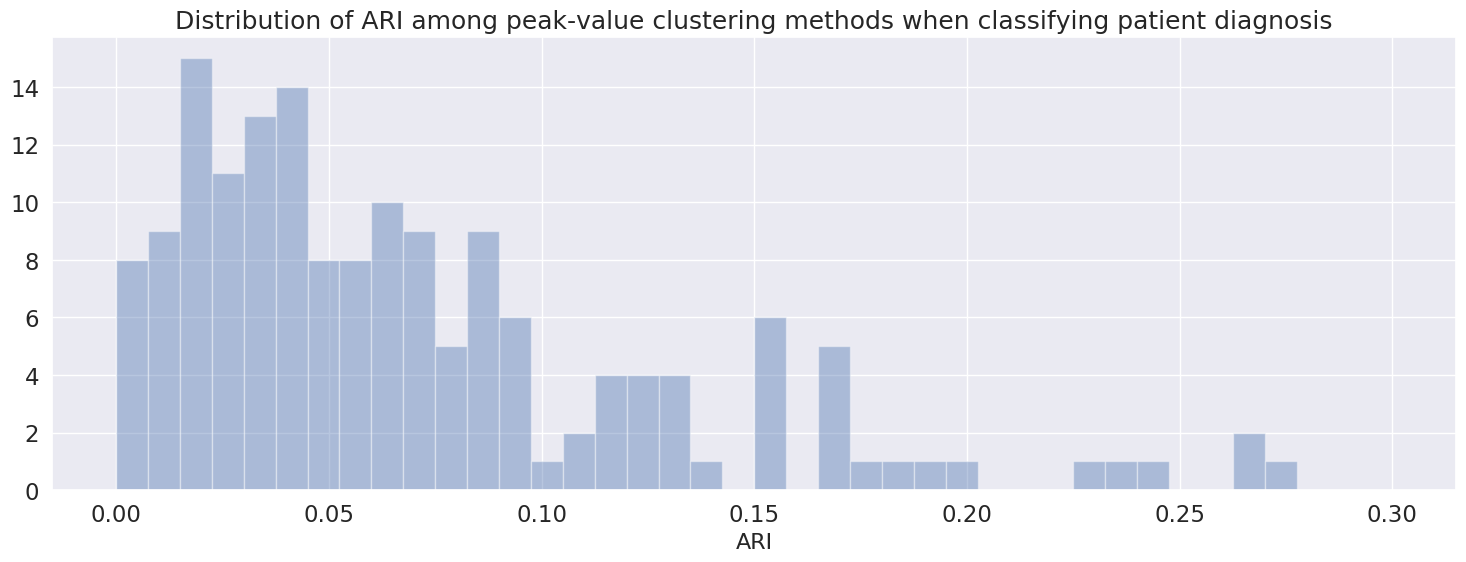
\includegraphics[width=\textwidth]{results/pvc-ind-ari.png}
    %% Creator: Matplotlib, PGF backend
%%
%% To include the figure in your LaTeX document, write
%%   \input{<filename>.pgf}
%%
%% Make sure the required packages are loaded in your preamble
%%   \usepackage{pgf}
%%
%% Figures using additional raster images can only be included by \input if
%% they are in the same directory as the main LaTeX file. For loading figures
%% from other directories you can use the `import` package
%%   \usepackage{import}
%% and then include the figures with
%%   \import{<path to file>}{<filename>.pgf}
%%
%% Matplotlib used the following preamble
%%
\begingroup%
\makeatletter%
\begin{pgfpicture}%
\pgfpathrectangle{\pgfpointorigin}{\pgfqpoint{6.340000in}{2.340000in}}%
\pgfusepath{use as bounding box, clip}%
\begin{pgfscope}%
\pgfsetbuttcap%
\pgfsetmiterjoin%
\definecolor{currentfill}{rgb}{1.000000,1.000000,1.000000}%
\pgfsetfillcolor{currentfill}%
\pgfsetlinewidth{0.000000pt}%
\definecolor{currentstroke}{rgb}{1.000000,1.000000,1.000000}%
\pgfsetstrokecolor{currentstroke}%
\pgfsetdash{}{0pt}%
\pgfpathmoveto{\pgfqpoint{0.000000in}{-0.000000in}}%
\pgfpathlineto{\pgfqpoint{6.340000in}{-0.000000in}}%
\pgfpathlineto{\pgfqpoint{6.340000in}{2.340000in}}%
\pgfpathlineto{\pgfqpoint{0.000000in}{2.340000in}}%
\pgfpathclose%
\pgfusepath{fill}%
\end{pgfscope}%
\begin{pgfscope}%
\pgfsetbuttcap%
\pgfsetmiterjoin%
\definecolor{currentfill}{rgb}{0.917647,0.917647,0.949020}%
\pgfsetfillcolor{currentfill}%
\pgfsetlinewidth{0.000000pt}%
\definecolor{currentstroke}{rgb}{0.000000,0.000000,0.000000}%
\pgfsetstrokecolor{currentstroke}%
\pgfsetstrokeopacity{0.000000}%
\pgfsetdash{}{0pt}%
\pgfpathmoveto{\pgfqpoint{0.574769in}{0.557870in}}%
\pgfpathlineto{\pgfqpoint{6.240000in}{0.557870in}}%
\pgfpathlineto{\pgfqpoint{6.240000in}{2.240000in}}%
\pgfpathlineto{\pgfqpoint{0.574769in}{2.240000in}}%
\pgfpathclose%
\pgfusepath{fill}%
\end{pgfscope}%
\begin{pgfscope}%
\pgfpathrectangle{\pgfqpoint{0.574769in}{0.557870in}}{\pgfqpoint{5.665231in}{1.682130in}}%
\pgfusepath{clip}%
\pgfsetroundcap%
\pgfsetroundjoin%
\pgfsetlinewidth{1.003750pt}%
\definecolor{currentstroke}{rgb}{1.000000,1.000000,1.000000}%
\pgfsetstrokecolor{currentstroke}%
\pgfsetdash{}{0pt}%
\pgfpathmoveto{\pgfqpoint{1.053663in}{0.557870in}}%
\pgfpathlineto{\pgfqpoint{1.053663in}{2.240000in}}%
\pgfusepath{stroke}%
\end{pgfscope}%
\begin{pgfscope}%
\definecolor{textcolor}{rgb}{0.150000,0.150000,0.150000}%
\pgfsetstrokecolor{textcolor}%
\pgfsetfillcolor{textcolor}%
\pgftext[x=1.053663in,y=0.425926in,,top]{\color{textcolor}\sffamily\fontsize{11.000000}{13.200000}\selectfont \(\displaystyle -0.05\)}%
\end{pgfscope}%
\begin{pgfscope}%
\pgfpathrectangle{\pgfqpoint{0.574769in}{0.557870in}}{\pgfqpoint{5.665231in}{1.682130in}}%
\pgfusepath{clip}%
\pgfsetroundcap%
\pgfsetroundjoin%
\pgfsetlinewidth{1.003750pt}%
\definecolor{currentstroke}{rgb}{1.000000,1.000000,1.000000}%
\pgfsetstrokecolor{currentstroke}%
\pgfsetdash{}{0pt}%
\pgfpathmoveto{\pgfqpoint{1.815006in}{0.557870in}}%
\pgfpathlineto{\pgfqpoint{1.815006in}{2.240000in}}%
\pgfusepath{stroke}%
\end{pgfscope}%
\begin{pgfscope}%
\definecolor{textcolor}{rgb}{0.150000,0.150000,0.150000}%
\pgfsetstrokecolor{textcolor}%
\pgfsetfillcolor{textcolor}%
\pgftext[x=1.815006in,y=0.425926in,,top]{\color{textcolor}\sffamily\fontsize{11.000000}{13.200000}\selectfont \(\displaystyle 0.00\)}%
\end{pgfscope}%
\begin{pgfscope}%
\pgfpathrectangle{\pgfqpoint{0.574769in}{0.557870in}}{\pgfqpoint{5.665231in}{1.682130in}}%
\pgfusepath{clip}%
\pgfsetroundcap%
\pgfsetroundjoin%
\pgfsetlinewidth{1.003750pt}%
\definecolor{currentstroke}{rgb}{1.000000,1.000000,1.000000}%
\pgfsetstrokecolor{currentstroke}%
\pgfsetdash{}{0pt}%
\pgfpathmoveto{\pgfqpoint{2.576349in}{0.557870in}}%
\pgfpathlineto{\pgfqpoint{2.576349in}{2.240000in}}%
\pgfusepath{stroke}%
\end{pgfscope}%
\begin{pgfscope}%
\definecolor{textcolor}{rgb}{0.150000,0.150000,0.150000}%
\pgfsetstrokecolor{textcolor}%
\pgfsetfillcolor{textcolor}%
\pgftext[x=2.576349in,y=0.425926in,,top]{\color{textcolor}\sffamily\fontsize{11.000000}{13.200000}\selectfont \(\displaystyle 0.05\)}%
\end{pgfscope}%
\begin{pgfscope}%
\pgfpathrectangle{\pgfqpoint{0.574769in}{0.557870in}}{\pgfqpoint{5.665231in}{1.682130in}}%
\pgfusepath{clip}%
\pgfsetroundcap%
\pgfsetroundjoin%
\pgfsetlinewidth{1.003750pt}%
\definecolor{currentstroke}{rgb}{1.000000,1.000000,1.000000}%
\pgfsetstrokecolor{currentstroke}%
\pgfsetdash{}{0pt}%
\pgfpathmoveto{\pgfqpoint{3.337692in}{0.557870in}}%
\pgfpathlineto{\pgfqpoint{3.337692in}{2.240000in}}%
\pgfusepath{stroke}%
\end{pgfscope}%
\begin{pgfscope}%
\definecolor{textcolor}{rgb}{0.150000,0.150000,0.150000}%
\pgfsetstrokecolor{textcolor}%
\pgfsetfillcolor{textcolor}%
\pgftext[x=3.337692in,y=0.425926in,,top]{\color{textcolor}\sffamily\fontsize{11.000000}{13.200000}\selectfont \(\displaystyle 0.10\)}%
\end{pgfscope}%
\begin{pgfscope}%
\pgfpathrectangle{\pgfqpoint{0.574769in}{0.557870in}}{\pgfqpoint{5.665231in}{1.682130in}}%
\pgfusepath{clip}%
\pgfsetroundcap%
\pgfsetroundjoin%
\pgfsetlinewidth{1.003750pt}%
\definecolor{currentstroke}{rgb}{1.000000,1.000000,1.000000}%
\pgfsetstrokecolor{currentstroke}%
\pgfsetdash{}{0pt}%
\pgfpathmoveto{\pgfqpoint{4.099035in}{0.557870in}}%
\pgfpathlineto{\pgfqpoint{4.099035in}{2.240000in}}%
\pgfusepath{stroke}%
\end{pgfscope}%
\begin{pgfscope}%
\definecolor{textcolor}{rgb}{0.150000,0.150000,0.150000}%
\pgfsetstrokecolor{textcolor}%
\pgfsetfillcolor{textcolor}%
\pgftext[x=4.099035in,y=0.425926in,,top]{\color{textcolor}\sffamily\fontsize{11.000000}{13.200000}\selectfont \(\displaystyle 0.15\)}%
\end{pgfscope}%
\begin{pgfscope}%
\pgfpathrectangle{\pgfqpoint{0.574769in}{0.557870in}}{\pgfqpoint{5.665231in}{1.682130in}}%
\pgfusepath{clip}%
\pgfsetroundcap%
\pgfsetroundjoin%
\pgfsetlinewidth{1.003750pt}%
\definecolor{currentstroke}{rgb}{1.000000,1.000000,1.000000}%
\pgfsetstrokecolor{currentstroke}%
\pgfsetdash{}{0pt}%
\pgfpathmoveto{\pgfqpoint{4.860378in}{0.557870in}}%
\pgfpathlineto{\pgfqpoint{4.860378in}{2.240000in}}%
\pgfusepath{stroke}%
\end{pgfscope}%
\begin{pgfscope}%
\definecolor{textcolor}{rgb}{0.150000,0.150000,0.150000}%
\pgfsetstrokecolor{textcolor}%
\pgfsetfillcolor{textcolor}%
\pgftext[x=4.860378in,y=0.425926in,,top]{\color{textcolor}\sffamily\fontsize{11.000000}{13.200000}\selectfont \(\displaystyle 0.20\)}%
\end{pgfscope}%
\begin{pgfscope}%
\pgfpathrectangle{\pgfqpoint{0.574769in}{0.557870in}}{\pgfqpoint{5.665231in}{1.682130in}}%
\pgfusepath{clip}%
\pgfsetroundcap%
\pgfsetroundjoin%
\pgfsetlinewidth{1.003750pt}%
\definecolor{currentstroke}{rgb}{1.000000,1.000000,1.000000}%
\pgfsetstrokecolor{currentstroke}%
\pgfsetdash{}{0pt}%
\pgfpathmoveto{\pgfqpoint{5.621721in}{0.557870in}}%
\pgfpathlineto{\pgfqpoint{5.621721in}{2.240000in}}%
\pgfusepath{stroke}%
\end{pgfscope}%
\begin{pgfscope}%
\definecolor{textcolor}{rgb}{0.150000,0.150000,0.150000}%
\pgfsetstrokecolor{textcolor}%
\pgfsetfillcolor{textcolor}%
\pgftext[x=5.621721in,y=0.425926in,,top]{\color{textcolor}\sffamily\fontsize{11.000000}{13.200000}\selectfont \(\displaystyle 0.25\)}%
\end{pgfscope}%
\begin{pgfscope}%
\definecolor{textcolor}{rgb}{0.150000,0.150000,0.150000}%
\pgfsetstrokecolor{textcolor}%
\pgfsetfillcolor{textcolor}%
\pgftext[x=3.407384in,y=0.235185in,,top]{\color{textcolor}\sffamily\fontsize{11.000000}{13.200000}\selectfont ARI}%
\end{pgfscope}%
\begin{pgfscope}%
\pgfpathrectangle{\pgfqpoint{0.574769in}{0.557870in}}{\pgfqpoint{5.665231in}{1.682130in}}%
\pgfusepath{clip}%
\pgfsetroundcap%
\pgfsetroundjoin%
\pgfsetlinewidth{1.003750pt}%
\definecolor{currentstroke}{rgb}{1.000000,1.000000,1.000000}%
\pgfsetstrokecolor{currentstroke}%
\pgfsetdash{}{0pt}%
\pgfpathmoveto{\pgfqpoint{0.574769in}{0.557870in}}%
\pgfpathlineto{\pgfqpoint{6.240000in}{0.557870in}}%
\pgfusepath{stroke}%
\end{pgfscope}%
\begin{pgfscope}%
\definecolor{textcolor}{rgb}{0.150000,0.150000,0.150000}%
\pgfsetstrokecolor{textcolor}%
\pgfsetfillcolor{textcolor}%
\pgftext[x=0.366783in,y=0.505064in,left,base]{\color{textcolor}\sffamily\fontsize{11.000000}{13.200000}\selectfont \(\displaystyle 0\)}%
\end{pgfscope}%
\begin{pgfscope}%
\pgfpathrectangle{\pgfqpoint{0.574769in}{0.557870in}}{\pgfqpoint{5.665231in}{1.682130in}}%
\pgfusepath{clip}%
\pgfsetroundcap%
\pgfsetroundjoin%
\pgfsetlinewidth{1.003750pt}%
\definecolor{currentstroke}{rgb}{1.000000,1.000000,1.000000}%
\pgfsetstrokecolor{currentstroke}%
\pgfsetdash{}{0pt}%
\pgfpathmoveto{\pgfqpoint{0.574769in}{0.898727in}}%
\pgfpathlineto{\pgfqpoint{6.240000in}{0.898727in}}%
\pgfusepath{stroke}%
\end{pgfscope}%
\begin{pgfscope}%
\definecolor{textcolor}{rgb}{0.150000,0.150000,0.150000}%
\pgfsetstrokecolor{textcolor}%
\pgfsetfillcolor{textcolor}%
\pgftext[x=0.290741in,y=0.845921in,left,base]{\color{textcolor}\sffamily\fontsize{11.000000}{13.200000}\selectfont \(\displaystyle 10\)}%
\end{pgfscope}%
\begin{pgfscope}%
\pgfpathrectangle{\pgfqpoint{0.574769in}{0.557870in}}{\pgfqpoint{5.665231in}{1.682130in}}%
\pgfusepath{clip}%
\pgfsetroundcap%
\pgfsetroundjoin%
\pgfsetlinewidth{1.003750pt}%
\definecolor{currentstroke}{rgb}{1.000000,1.000000,1.000000}%
\pgfsetstrokecolor{currentstroke}%
\pgfsetdash{}{0pt}%
\pgfpathmoveto{\pgfqpoint{0.574769in}{1.239584in}}%
\pgfpathlineto{\pgfqpoint{6.240000in}{1.239584in}}%
\pgfusepath{stroke}%
\end{pgfscope}%
\begin{pgfscope}%
\definecolor{textcolor}{rgb}{0.150000,0.150000,0.150000}%
\pgfsetstrokecolor{textcolor}%
\pgfsetfillcolor{textcolor}%
\pgftext[x=0.290741in,y=1.186778in,left,base]{\color{textcolor}\sffamily\fontsize{11.000000}{13.200000}\selectfont \(\displaystyle 20\)}%
\end{pgfscope}%
\begin{pgfscope}%
\pgfpathrectangle{\pgfqpoint{0.574769in}{0.557870in}}{\pgfqpoint{5.665231in}{1.682130in}}%
\pgfusepath{clip}%
\pgfsetroundcap%
\pgfsetroundjoin%
\pgfsetlinewidth{1.003750pt}%
\definecolor{currentstroke}{rgb}{1.000000,1.000000,1.000000}%
\pgfsetstrokecolor{currentstroke}%
\pgfsetdash{}{0pt}%
\pgfpathmoveto{\pgfqpoint{0.574769in}{1.580442in}}%
\pgfpathlineto{\pgfqpoint{6.240000in}{1.580442in}}%
\pgfusepath{stroke}%
\end{pgfscope}%
\begin{pgfscope}%
\definecolor{textcolor}{rgb}{0.150000,0.150000,0.150000}%
\pgfsetstrokecolor{textcolor}%
\pgfsetfillcolor{textcolor}%
\pgftext[x=0.290741in,y=1.527635in,left,base]{\color{textcolor}\sffamily\fontsize{11.000000}{13.200000}\selectfont \(\displaystyle 30\)}%
\end{pgfscope}%
\begin{pgfscope}%
\pgfpathrectangle{\pgfqpoint{0.574769in}{0.557870in}}{\pgfqpoint{5.665231in}{1.682130in}}%
\pgfusepath{clip}%
\pgfsetroundcap%
\pgfsetroundjoin%
\pgfsetlinewidth{1.003750pt}%
\definecolor{currentstroke}{rgb}{1.000000,1.000000,1.000000}%
\pgfsetstrokecolor{currentstroke}%
\pgfsetdash{}{0pt}%
\pgfpathmoveto{\pgfqpoint{0.574769in}{1.921299in}}%
\pgfpathlineto{\pgfqpoint{6.240000in}{1.921299in}}%
\pgfusepath{stroke}%
\end{pgfscope}%
\begin{pgfscope}%
\definecolor{textcolor}{rgb}{0.150000,0.150000,0.150000}%
\pgfsetstrokecolor{textcolor}%
\pgfsetfillcolor{textcolor}%
\pgftext[x=0.290741in,y=1.868492in,left,base]{\color{textcolor}\sffamily\fontsize{11.000000}{13.200000}\selectfont \(\displaystyle 40\)}%
\end{pgfscope}%
\begin{pgfscope}%
\definecolor{textcolor}{rgb}{0.150000,0.150000,0.150000}%
\pgfsetstrokecolor{textcolor}%
\pgfsetfillcolor{textcolor}%
\pgftext[x=0.235185in,y=1.398935in,,bottom,rotate=90.000000]{\color{textcolor}\sffamily\fontsize{11.000000}{13.200000}\selectfont Occurance}%
\end{pgfscope}%
\begin{pgfscope}%
\pgfpathrectangle{\pgfqpoint{0.574769in}{0.557870in}}{\pgfqpoint{5.665231in}{1.682130in}}%
\pgfusepath{clip}%
\pgfsetbuttcap%
\pgfsetmiterjoin%
\definecolor{currentfill}{rgb}{0.298039,0.447059,0.690196}%
\pgfsetfillcolor{currentfill}%
\pgfsetfillopacity{0.400000}%
\pgfsetlinewidth{1.003750pt}%
\definecolor{currentstroke}{rgb}{1.000000,1.000000,1.000000}%
\pgfsetstrokecolor{currentstroke}%
\pgfsetstrokeopacity{0.400000}%
\pgfsetdash{}{0pt}%
\pgfpathmoveto{\pgfqpoint{0.832279in}{0.557870in}}%
\pgfpathlineto{\pgfqpoint{1.228449in}{0.557870in}}%
\pgfpathlineto{\pgfqpoint{1.228449in}{1.171413in}}%
\pgfpathlineto{\pgfqpoint{0.832279in}{1.171413in}}%
\pgfpathclose%
\pgfusepath{stroke,fill}%
\end{pgfscope}%
\begin{pgfscope}%
\pgfpathrectangle{\pgfqpoint{0.574769in}{0.557870in}}{\pgfqpoint{5.665231in}{1.682130in}}%
\pgfusepath{clip}%
\pgfsetbuttcap%
\pgfsetmiterjoin%
\definecolor{currentfill}{rgb}{0.298039,0.447059,0.690196}%
\pgfsetfillcolor{currentfill}%
\pgfsetfillopacity{0.400000}%
\pgfsetlinewidth{1.003750pt}%
\definecolor{currentstroke}{rgb}{1.000000,1.000000,1.000000}%
\pgfsetstrokecolor{currentstroke}%
\pgfsetstrokeopacity{0.400000}%
\pgfsetdash{}{0pt}%
\pgfpathmoveto{\pgfqpoint{1.228449in}{0.557870in}}%
\pgfpathlineto{\pgfqpoint{1.624619in}{0.557870in}}%
\pgfpathlineto{\pgfqpoint{1.624619in}{1.239584in}}%
\pgfpathlineto{\pgfqpoint{1.228449in}{1.239584in}}%
\pgfpathclose%
\pgfusepath{stroke,fill}%
\end{pgfscope}%
\begin{pgfscope}%
\pgfpathrectangle{\pgfqpoint{0.574769in}{0.557870in}}{\pgfqpoint{5.665231in}{1.682130in}}%
\pgfusepath{clip}%
\pgfsetbuttcap%
\pgfsetmiterjoin%
\definecolor{currentfill}{rgb}{0.298039,0.447059,0.690196}%
\pgfsetfillcolor{currentfill}%
\pgfsetfillopacity{0.400000}%
\pgfsetlinewidth{1.003750pt}%
\definecolor{currentstroke}{rgb}{1.000000,1.000000,1.000000}%
\pgfsetstrokecolor{currentstroke}%
\pgfsetstrokeopacity{0.400000}%
\pgfsetdash{}{0pt}%
\pgfpathmoveto{\pgfqpoint{1.624619in}{0.557870in}}%
\pgfpathlineto{\pgfqpoint{2.020789in}{0.557870in}}%
\pgfpathlineto{\pgfqpoint{2.020789in}{1.580442in}}%
\pgfpathlineto{\pgfqpoint{1.624619in}{1.580442in}}%
\pgfpathclose%
\pgfusepath{stroke,fill}%
\end{pgfscope}%
\begin{pgfscope}%
\pgfpathrectangle{\pgfqpoint{0.574769in}{0.557870in}}{\pgfqpoint{5.665231in}{1.682130in}}%
\pgfusepath{clip}%
\pgfsetbuttcap%
\pgfsetmiterjoin%
\definecolor{currentfill}{rgb}{0.298039,0.447059,0.690196}%
\pgfsetfillcolor{currentfill}%
\pgfsetfillopacity{0.400000}%
\pgfsetlinewidth{1.003750pt}%
\definecolor{currentstroke}{rgb}{1.000000,1.000000,1.000000}%
\pgfsetstrokecolor{currentstroke}%
\pgfsetstrokeopacity{0.400000}%
\pgfsetdash{}{0pt}%
\pgfpathmoveto{\pgfqpoint{2.020789in}{0.557870in}}%
\pgfpathlineto{\pgfqpoint{2.416959in}{0.557870in}}%
\pgfpathlineto{\pgfqpoint{2.416959in}{2.159899in}}%
\pgfpathlineto{\pgfqpoint{2.020789in}{2.159899in}}%
\pgfpathclose%
\pgfusepath{stroke,fill}%
\end{pgfscope}%
\begin{pgfscope}%
\pgfpathrectangle{\pgfqpoint{0.574769in}{0.557870in}}{\pgfqpoint{5.665231in}{1.682130in}}%
\pgfusepath{clip}%
\pgfsetbuttcap%
\pgfsetmiterjoin%
\definecolor{currentfill}{rgb}{0.298039,0.447059,0.690196}%
\pgfsetfillcolor{currentfill}%
\pgfsetfillopacity{0.400000}%
\pgfsetlinewidth{1.003750pt}%
\definecolor{currentstroke}{rgb}{1.000000,1.000000,1.000000}%
\pgfsetstrokecolor{currentstroke}%
\pgfsetstrokeopacity{0.400000}%
\pgfsetdash{}{0pt}%
\pgfpathmoveto{\pgfqpoint{2.416959in}{0.557870in}}%
\pgfpathlineto{\pgfqpoint{2.813129in}{0.557870in}}%
\pgfpathlineto{\pgfqpoint{2.813129in}{1.648613in}}%
\pgfpathlineto{\pgfqpoint{2.416959in}{1.648613in}}%
\pgfpathclose%
\pgfusepath{stroke,fill}%
\end{pgfscope}%
\begin{pgfscope}%
\pgfpathrectangle{\pgfqpoint{0.574769in}{0.557870in}}{\pgfqpoint{5.665231in}{1.682130in}}%
\pgfusepath{clip}%
\pgfsetbuttcap%
\pgfsetmiterjoin%
\definecolor{currentfill}{rgb}{0.298039,0.447059,0.690196}%
\pgfsetfillcolor{currentfill}%
\pgfsetfillopacity{0.400000}%
\pgfsetlinewidth{1.003750pt}%
\definecolor{currentstroke}{rgb}{1.000000,1.000000,1.000000}%
\pgfsetstrokecolor{currentstroke}%
\pgfsetstrokeopacity{0.400000}%
\pgfsetdash{}{0pt}%
\pgfpathmoveto{\pgfqpoint{2.813129in}{0.557870in}}%
\pgfpathlineto{\pgfqpoint{3.209299in}{0.557870in}}%
\pgfpathlineto{\pgfqpoint{3.209299in}{1.444099in}}%
\pgfpathlineto{\pgfqpoint{2.813129in}{1.444099in}}%
\pgfpathclose%
\pgfusepath{stroke,fill}%
\end{pgfscope}%
\begin{pgfscope}%
\pgfpathrectangle{\pgfqpoint{0.574769in}{0.557870in}}{\pgfqpoint{5.665231in}{1.682130in}}%
\pgfusepath{clip}%
\pgfsetbuttcap%
\pgfsetmiterjoin%
\definecolor{currentfill}{rgb}{0.298039,0.447059,0.690196}%
\pgfsetfillcolor{currentfill}%
\pgfsetfillopacity{0.400000}%
\pgfsetlinewidth{1.003750pt}%
\definecolor{currentstroke}{rgb}{1.000000,1.000000,1.000000}%
\pgfsetstrokecolor{currentstroke}%
\pgfsetstrokeopacity{0.400000}%
\pgfsetdash{}{0pt}%
\pgfpathmoveto{\pgfqpoint{3.209299in}{0.557870in}}%
\pgfpathlineto{\pgfqpoint{3.605469in}{0.557870in}}%
\pgfpathlineto{\pgfqpoint{3.605469in}{0.966899in}}%
\pgfpathlineto{\pgfqpoint{3.209299in}{0.966899in}}%
\pgfpathclose%
\pgfusepath{stroke,fill}%
\end{pgfscope}%
\begin{pgfscope}%
\pgfpathrectangle{\pgfqpoint{0.574769in}{0.557870in}}{\pgfqpoint{5.665231in}{1.682130in}}%
\pgfusepath{clip}%
\pgfsetbuttcap%
\pgfsetmiterjoin%
\definecolor{currentfill}{rgb}{0.298039,0.447059,0.690196}%
\pgfsetfillcolor{currentfill}%
\pgfsetfillopacity{0.400000}%
\pgfsetlinewidth{1.003750pt}%
\definecolor{currentstroke}{rgb}{1.000000,1.000000,1.000000}%
\pgfsetstrokecolor{currentstroke}%
\pgfsetstrokeopacity{0.400000}%
\pgfsetdash{}{0pt}%
\pgfpathmoveto{\pgfqpoint{3.605469in}{0.557870in}}%
\pgfpathlineto{\pgfqpoint{4.001639in}{0.557870in}}%
\pgfpathlineto{\pgfqpoint{4.001639in}{0.898727in}}%
\pgfpathlineto{\pgfqpoint{3.605469in}{0.898727in}}%
\pgfpathclose%
\pgfusepath{stroke,fill}%
\end{pgfscope}%
\begin{pgfscope}%
\pgfpathrectangle{\pgfqpoint{0.574769in}{0.557870in}}{\pgfqpoint{5.665231in}{1.682130in}}%
\pgfusepath{clip}%
\pgfsetbuttcap%
\pgfsetmiterjoin%
\definecolor{currentfill}{rgb}{0.298039,0.447059,0.690196}%
\pgfsetfillcolor{currentfill}%
\pgfsetfillopacity{0.400000}%
\pgfsetlinewidth{1.003750pt}%
\definecolor{currentstroke}{rgb}{1.000000,1.000000,1.000000}%
\pgfsetstrokecolor{currentstroke}%
\pgfsetstrokeopacity{0.400000}%
\pgfsetdash{}{0pt}%
\pgfpathmoveto{\pgfqpoint{4.001639in}{0.557870in}}%
\pgfpathlineto{\pgfqpoint{4.397809in}{0.557870in}}%
\pgfpathlineto{\pgfqpoint{4.397809in}{0.796470in}}%
\pgfpathlineto{\pgfqpoint{4.001639in}{0.796470in}}%
\pgfpathclose%
\pgfusepath{stroke,fill}%
\end{pgfscope}%
\begin{pgfscope}%
\pgfpathrectangle{\pgfqpoint{0.574769in}{0.557870in}}{\pgfqpoint{5.665231in}{1.682130in}}%
\pgfusepath{clip}%
\pgfsetbuttcap%
\pgfsetmiterjoin%
\definecolor{currentfill}{rgb}{0.298039,0.447059,0.690196}%
\pgfsetfillcolor{currentfill}%
\pgfsetfillopacity{0.400000}%
\pgfsetlinewidth{1.003750pt}%
\definecolor{currentstroke}{rgb}{1.000000,1.000000,1.000000}%
\pgfsetstrokecolor{currentstroke}%
\pgfsetstrokeopacity{0.400000}%
\pgfsetdash{}{0pt}%
\pgfpathmoveto{\pgfqpoint{4.397809in}{0.557870in}}%
\pgfpathlineto{\pgfqpoint{4.793979in}{0.557870in}}%
\pgfpathlineto{\pgfqpoint{4.793979in}{0.796470in}}%
\pgfpathlineto{\pgfqpoint{4.397809in}{0.796470in}}%
\pgfpathclose%
\pgfusepath{stroke,fill}%
\end{pgfscope}%
\begin{pgfscope}%
\pgfpathrectangle{\pgfqpoint{0.574769in}{0.557870in}}{\pgfqpoint{5.665231in}{1.682130in}}%
\pgfusepath{clip}%
\pgfsetbuttcap%
\pgfsetmiterjoin%
\definecolor{currentfill}{rgb}{0.298039,0.447059,0.690196}%
\pgfsetfillcolor{currentfill}%
\pgfsetfillopacity{0.400000}%
\pgfsetlinewidth{1.003750pt}%
\definecolor{currentstroke}{rgb}{1.000000,1.000000,1.000000}%
\pgfsetstrokecolor{currentstroke}%
\pgfsetstrokeopacity{0.400000}%
\pgfsetdash{}{0pt}%
\pgfpathmoveto{\pgfqpoint{4.793979in}{0.557870in}}%
\pgfpathlineto{\pgfqpoint{5.190149in}{0.557870in}}%
\pgfpathlineto{\pgfqpoint{5.190149in}{0.591956in}}%
\pgfpathlineto{\pgfqpoint{4.793979in}{0.591956in}}%
\pgfpathclose%
\pgfusepath{stroke,fill}%
\end{pgfscope}%
\begin{pgfscope}%
\pgfpathrectangle{\pgfqpoint{0.574769in}{0.557870in}}{\pgfqpoint{5.665231in}{1.682130in}}%
\pgfusepath{clip}%
\pgfsetbuttcap%
\pgfsetmiterjoin%
\definecolor{currentfill}{rgb}{0.298039,0.447059,0.690196}%
\pgfsetfillcolor{currentfill}%
\pgfsetfillopacity{0.400000}%
\pgfsetlinewidth{1.003750pt}%
\definecolor{currentstroke}{rgb}{1.000000,1.000000,1.000000}%
\pgfsetstrokecolor{currentstroke}%
\pgfsetstrokeopacity{0.400000}%
\pgfsetdash{}{0pt}%
\pgfpathmoveto{\pgfqpoint{5.190149in}{0.557870in}}%
\pgfpathlineto{\pgfqpoint{5.586319in}{0.557870in}}%
\pgfpathlineto{\pgfqpoint{5.586319in}{0.660127in}}%
\pgfpathlineto{\pgfqpoint{5.190149in}{0.660127in}}%
\pgfpathclose%
\pgfusepath{stroke,fill}%
\end{pgfscope}%
\begin{pgfscope}%
\pgfpathrectangle{\pgfqpoint{0.574769in}{0.557870in}}{\pgfqpoint{5.665231in}{1.682130in}}%
\pgfusepath{clip}%
\pgfsetbuttcap%
\pgfsetmiterjoin%
\definecolor{currentfill}{rgb}{0.298039,0.447059,0.690196}%
\pgfsetfillcolor{currentfill}%
\pgfsetfillopacity{0.400000}%
\pgfsetlinewidth{1.003750pt}%
\definecolor{currentstroke}{rgb}{1.000000,1.000000,1.000000}%
\pgfsetstrokecolor{currentstroke}%
\pgfsetstrokeopacity{0.400000}%
\pgfsetdash{}{0pt}%
\pgfpathmoveto{\pgfqpoint{5.586319in}{0.557870in}}%
\pgfpathlineto{\pgfqpoint{5.982489in}{0.557870in}}%
\pgfpathlineto{\pgfqpoint{5.982489in}{0.660127in}}%
\pgfpathlineto{\pgfqpoint{5.586319in}{0.660127in}}%
\pgfpathclose%
\pgfusepath{stroke,fill}%
\end{pgfscope}%
\begin{pgfscope}%
\pgfsetrectcap%
\pgfsetmiterjoin%
\pgfsetlinewidth{1.254687pt}%
\definecolor{currentstroke}{rgb}{1.000000,1.000000,1.000000}%
\pgfsetstrokecolor{currentstroke}%
\pgfsetdash{}{0pt}%
\pgfpathmoveto{\pgfqpoint{0.574769in}{0.557870in}}%
\pgfpathlineto{\pgfqpoint{0.574769in}{2.240000in}}%
\pgfusepath{stroke}%
\end{pgfscope}%
\begin{pgfscope}%
\pgfsetrectcap%
\pgfsetmiterjoin%
\pgfsetlinewidth{1.254687pt}%
\definecolor{currentstroke}{rgb}{1.000000,1.000000,1.000000}%
\pgfsetstrokecolor{currentstroke}%
\pgfsetdash{}{0pt}%
\pgfpathmoveto{\pgfqpoint{6.240000in}{0.557870in}}%
\pgfpathlineto{\pgfqpoint{6.240000in}{2.240000in}}%
\pgfusepath{stroke}%
\end{pgfscope}%
\begin{pgfscope}%
\pgfsetrectcap%
\pgfsetmiterjoin%
\pgfsetlinewidth{1.254687pt}%
\definecolor{currentstroke}{rgb}{1.000000,1.000000,1.000000}%
\pgfsetstrokecolor{currentstroke}%
\pgfsetdash{}{0pt}%
\pgfpathmoveto{\pgfqpoint{0.574769in}{0.557870in}}%
\pgfpathlineto{\pgfqpoint{6.240000in}{0.557870in}}%
\pgfusepath{stroke}%
\end{pgfscope}%
\begin{pgfscope}%
\pgfsetrectcap%
\pgfsetmiterjoin%
\pgfsetlinewidth{1.254687pt}%
\definecolor{currentstroke}{rgb}{1.000000,1.000000,1.000000}%
\pgfsetstrokecolor{currentstroke}%
\pgfsetdash{}{0pt}%
\pgfpathmoveto{\pgfqpoint{0.574769in}{2.240000in}}%
\pgfpathlineto{\pgfqpoint{6.240000in}{2.240000in}}%
\pgfusepath{stroke}%
\end{pgfscope}%
\end{pgfpicture}%
\makeatother%
\endgroup%

    \caption{ARI distribution of PVC methods when classifying patient diagnoses.}
    \label{fig:pvc_ind_ari}
\end{figure}

\newpage

\subsection{Deep Neural Network}

\begin{figure}[htb]
    \centering
    % \includegraphics[width=\textwidth]{results/dl_ind_dor_sens_spec_dist.png}
    %% Creator: Matplotlib, PGF backend
%%
%% To include the figure in your LaTeX document, write
%%   \input{<filename>.pgf}
%%
%% Make sure the required packages are loaded in your preamble
%%   \usepackage{pgf}
%%
%% Figures using additional raster images can only be included by \input if
%% they are in the same directory as the main LaTeX file. For loading figures
%% from other directories you can use the `import` package
%%   \usepackage{import}
%% and then include the figures with
%%   \import{<path to file>}{<filename>.pgf}
%%
%% Matplotlib used the following preamble
%%
\begingroup%
\makeatletter%
\begin{pgfpicture}%
\pgfpathrectangle{\pgfpointorigin}{\pgfqpoint{6.363231in}{2.340000in}}%
\pgfusepath{use as bounding box, clip}%
\begin{pgfscope}%
\pgfsetbuttcap%
\pgfsetmiterjoin%
\definecolor{currentfill}{rgb}{1.000000,1.000000,1.000000}%
\pgfsetfillcolor{currentfill}%
\pgfsetlinewidth{0.000000pt}%
\definecolor{currentstroke}{rgb}{1.000000,1.000000,1.000000}%
\pgfsetstrokecolor{currentstroke}%
\pgfsetdash{}{0pt}%
\pgfpathmoveto{\pgfqpoint{0.000000in}{-0.000000in}}%
\pgfpathlineto{\pgfqpoint{6.363231in}{-0.000000in}}%
\pgfpathlineto{\pgfqpoint{6.363231in}{2.340000in}}%
\pgfpathlineto{\pgfqpoint{0.000000in}{2.340000in}}%
\pgfpathclose%
\pgfusepath{fill}%
\end{pgfscope}%
\begin{pgfscope}%
\pgfsetbuttcap%
\pgfsetmiterjoin%
\definecolor{currentfill}{rgb}{0.917647,0.917647,0.949020}%
\pgfsetfillcolor{currentfill}%
\pgfsetlinewidth{0.000000pt}%
\definecolor{currentstroke}{rgb}{0.000000,0.000000,0.000000}%
\pgfsetstrokecolor{currentstroke}%
\pgfsetstrokeopacity{0.000000}%
\pgfsetdash{}{0pt}%
\pgfpathmoveto{\pgfqpoint{0.617014in}{0.557870in}}%
\pgfpathlineto{\pgfqpoint{3.080000in}{0.557870in}}%
\pgfpathlineto{\pgfqpoint{3.080000in}{2.042604in}}%
\pgfpathlineto{\pgfqpoint{0.617014in}{2.042604in}}%
\pgfpathclose%
\pgfusepath{fill}%
\end{pgfscope}%
\begin{pgfscope}%
\pgfpathrectangle{\pgfqpoint{0.617014in}{0.557870in}}{\pgfqpoint{2.462986in}{1.484734in}}%
\pgfusepath{clip}%
\pgfsetroundcap%
\pgfsetroundjoin%
\pgfsetlinewidth{1.003750pt}%
\definecolor{currentstroke}{rgb}{1.000000,1.000000,1.000000}%
\pgfsetstrokecolor{currentstroke}%
\pgfsetdash{}{0pt}%
\pgfpathmoveto{\pgfqpoint{0.728968in}{0.557870in}}%
\pgfpathlineto{\pgfqpoint{0.728968in}{2.042604in}}%
\pgfusepath{stroke}%
\end{pgfscope}%
\begin{pgfscope}%
\definecolor{textcolor}{rgb}{0.150000,0.150000,0.150000}%
\pgfsetstrokecolor{textcolor}%
\pgfsetfillcolor{textcolor}%
\pgftext[x=0.728968in,y=0.425926in,,top]{\color{textcolor}\sffamily\fontsize{11.000000}{13.200000}\selectfont \(\displaystyle -0.50\)}%
\end{pgfscope}%
\begin{pgfscope}%
\pgfpathrectangle{\pgfqpoint{0.617014in}{0.557870in}}{\pgfqpoint{2.462986in}{1.484734in}}%
\pgfusepath{clip}%
\pgfsetroundcap%
\pgfsetroundjoin%
\pgfsetlinewidth{1.003750pt}%
\definecolor{currentstroke}{rgb}{1.000000,1.000000,1.000000}%
\pgfsetstrokecolor{currentstroke}%
\pgfsetdash{}{0pt}%
\pgfpathmoveto{\pgfqpoint{1.288737in}{0.557870in}}%
\pgfpathlineto{\pgfqpoint{1.288737in}{2.042604in}}%
\pgfusepath{stroke}%
\end{pgfscope}%
\begin{pgfscope}%
\definecolor{textcolor}{rgb}{0.150000,0.150000,0.150000}%
\pgfsetstrokecolor{textcolor}%
\pgfsetfillcolor{textcolor}%
\pgftext[x=1.288737in,y=0.425926in,,top]{\color{textcolor}\sffamily\fontsize{11.000000}{13.200000}\selectfont \(\displaystyle -0.25\)}%
\end{pgfscope}%
\begin{pgfscope}%
\pgfpathrectangle{\pgfqpoint{0.617014in}{0.557870in}}{\pgfqpoint{2.462986in}{1.484734in}}%
\pgfusepath{clip}%
\pgfsetroundcap%
\pgfsetroundjoin%
\pgfsetlinewidth{1.003750pt}%
\definecolor{currentstroke}{rgb}{1.000000,1.000000,1.000000}%
\pgfsetstrokecolor{currentstroke}%
\pgfsetdash{}{0pt}%
\pgfpathmoveto{\pgfqpoint{1.848507in}{0.557870in}}%
\pgfpathlineto{\pgfqpoint{1.848507in}{2.042604in}}%
\pgfusepath{stroke}%
\end{pgfscope}%
\begin{pgfscope}%
\definecolor{textcolor}{rgb}{0.150000,0.150000,0.150000}%
\pgfsetstrokecolor{textcolor}%
\pgfsetfillcolor{textcolor}%
\pgftext[x=1.848507in,y=0.425926in,,top]{\color{textcolor}\sffamily\fontsize{11.000000}{13.200000}\selectfont \(\displaystyle 0.00\)}%
\end{pgfscope}%
\begin{pgfscope}%
\pgfpathrectangle{\pgfqpoint{0.617014in}{0.557870in}}{\pgfqpoint{2.462986in}{1.484734in}}%
\pgfusepath{clip}%
\pgfsetroundcap%
\pgfsetroundjoin%
\pgfsetlinewidth{1.003750pt}%
\definecolor{currentstroke}{rgb}{1.000000,1.000000,1.000000}%
\pgfsetstrokecolor{currentstroke}%
\pgfsetdash{}{0pt}%
\pgfpathmoveto{\pgfqpoint{2.408277in}{0.557870in}}%
\pgfpathlineto{\pgfqpoint{2.408277in}{2.042604in}}%
\pgfusepath{stroke}%
\end{pgfscope}%
\begin{pgfscope}%
\definecolor{textcolor}{rgb}{0.150000,0.150000,0.150000}%
\pgfsetstrokecolor{textcolor}%
\pgfsetfillcolor{textcolor}%
\pgftext[x=2.408277in,y=0.425926in,,top]{\color{textcolor}\sffamily\fontsize{11.000000}{13.200000}\selectfont \(\displaystyle 0.25\)}%
\end{pgfscope}%
\begin{pgfscope}%
\pgfpathrectangle{\pgfqpoint{0.617014in}{0.557870in}}{\pgfqpoint{2.462986in}{1.484734in}}%
\pgfusepath{clip}%
\pgfsetroundcap%
\pgfsetroundjoin%
\pgfsetlinewidth{1.003750pt}%
\definecolor{currentstroke}{rgb}{1.000000,1.000000,1.000000}%
\pgfsetstrokecolor{currentstroke}%
\pgfsetdash{}{0pt}%
\pgfpathmoveto{\pgfqpoint{2.968046in}{0.557870in}}%
\pgfpathlineto{\pgfqpoint{2.968046in}{2.042604in}}%
\pgfusepath{stroke}%
\end{pgfscope}%
\begin{pgfscope}%
\definecolor{textcolor}{rgb}{0.150000,0.150000,0.150000}%
\pgfsetstrokecolor{textcolor}%
\pgfsetfillcolor{textcolor}%
\pgftext[x=2.968046in,y=0.425926in,,top]{\color{textcolor}\sffamily\fontsize{11.000000}{13.200000}\selectfont \(\displaystyle 0.50\)}%
\end{pgfscope}%
\begin{pgfscope}%
\definecolor{textcolor}{rgb}{0.150000,0.150000,0.150000}%
\pgfsetstrokecolor{textcolor}%
\pgfsetfillcolor{textcolor}%
\pgftext[x=1.848507in,y=0.235185in,,top]{\color{textcolor}\sffamily\fontsize{11.000000}{13.200000}\selectfont DOR}%
\end{pgfscope}%
\begin{pgfscope}%
\pgfpathrectangle{\pgfqpoint{0.617014in}{0.557870in}}{\pgfqpoint{2.462986in}{1.484734in}}%
\pgfusepath{clip}%
\pgfsetroundcap%
\pgfsetroundjoin%
\pgfsetlinewidth{1.003750pt}%
\definecolor{currentstroke}{rgb}{1.000000,1.000000,1.000000}%
\pgfsetstrokecolor{currentstroke}%
\pgfsetdash{}{0pt}%
\pgfpathmoveto{\pgfqpoint{0.617014in}{0.557870in}}%
\pgfpathlineto{\pgfqpoint{3.080000in}{0.557870in}}%
\pgfusepath{stroke}%
\end{pgfscope}%
\begin{pgfscope}%
\definecolor{textcolor}{rgb}{0.150000,0.150000,0.150000}%
\pgfsetstrokecolor{textcolor}%
\pgfsetfillcolor{textcolor}%
\pgftext[x=0.290741in,y=0.505064in,left,base]{\color{textcolor}\sffamily\fontsize{11.000000}{13.200000}\selectfont \(\displaystyle 0.0\)}%
\end{pgfscope}%
\begin{pgfscope}%
\pgfpathrectangle{\pgfqpoint{0.617014in}{0.557870in}}{\pgfqpoint{2.462986in}{1.484734in}}%
\pgfusepath{clip}%
\pgfsetroundcap%
\pgfsetroundjoin%
\pgfsetlinewidth{1.003750pt}%
\definecolor{currentstroke}{rgb}{1.000000,1.000000,1.000000}%
\pgfsetstrokecolor{currentstroke}%
\pgfsetdash{}{0pt}%
\pgfpathmoveto{\pgfqpoint{0.617014in}{1.264886in}}%
\pgfpathlineto{\pgfqpoint{3.080000in}{1.264886in}}%
\pgfusepath{stroke}%
\end{pgfscope}%
\begin{pgfscope}%
\definecolor{textcolor}{rgb}{0.150000,0.150000,0.150000}%
\pgfsetstrokecolor{textcolor}%
\pgfsetfillcolor{textcolor}%
\pgftext[x=0.290741in,y=1.212080in,left,base]{\color{textcolor}\sffamily\fontsize{11.000000}{13.200000}\selectfont \(\displaystyle 0.5\)}%
\end{pgfscope}%
\begin{pgfscope}%
\pgfpathrectangle{\pgfqpoint{0.617014in}{0.557870in}}{\pgfqpoint{2.462986in}{1.484734in}}%
\pgfusepath{clip}%
\pgfsetroundcap%
\pgfsetroundjoin%
\pgfsetlinewidth{1.003750pt}%
\definecolor{currentstroke}{rgb}{1.000000,1.000000,1.000000}%
\pgfsetstrokecolor{currentstroke}%
\pgfsetdash{}{0pt}%
\pgfpathmoveto{\pgfqpoint{0.617014in}{1.971903in}}%
\pgfpathlineto{\pgfqpoint{3.080000in}{1.971903in}}%
\pgfusepath{stroke}%
\end{pgfscope}%
\begin{pgfscope}%
\definecolor{textcolor}{rgb}{0.150000,0.150000,0.150000}%
\pgfsetstrokecolor{textcolor}%
\pgfsetfillcolor{textcolor}%
\pgftext[x=0.290741in,y=1.919096in,left,base]{\color{textcolor}\sffamily\fontsize{11.000000}{13.200000}\selectfont \(\displaystyle 1.0\)}%
\end{pgfscope}%
\begin{pgfscope}%
\definecolor{textcolor}{rgb}{0.150000,0.150000,0.150000}%
\pgfsetstrokecolor{textcolor}%
\pgfsetfillcolor{textcolor}%
\pgftext[x=0.235185in,y=1.300237in,,bottom,rotate=90.000000]{\color{textcolor}\sffamily\fontsize{11.000000}{13.200000}\selectfont Occurance}%
\end{pgfscope}%
\begin{pgfscope}%
\pgfpathrectangle{\pgfqpoint{0.617014in}{0.557870in}}{\pgfqpoint{2.462986in}{1.484734in}}%
\pgfusepath{clip}%
\pgfsetbuttcap%
\pgfsetmiterjoin%
\definecolor{currentfill}{rgb}{0.298039,0.447059,0.690196}%
\pgfsetfillcolor{currentfill}%
\pgfsetfillopacity{0.400000}%
\pgfsetlinewidth{1.003750pt}%
\definecolor{currentstroke}{rgb}{1.000000,1.000000,1.000000}%
\pgfsetstrokecolor{currentstroke}%
\pgfsetstrokeopacity{0.400000}%
\pgfsetdash{}{0pt}%
\pgfpathmoveto{\pgfqpoint{0.728968in}{0.557870in}}%
\pgfpathlineto{\pgfqpoint{0.952876in}{0.557870in}}%
\pgfpathlineto{\pgfqpoint{0.952876in}{0.557870in}}%
\pgfpathlineto{\pgfqpoint{0.728968in}{0.557870in}}%
\pgfpathclose%
\pgfusepath{stroke,fill}%
\end{pgfscope}%
\begin{pgfscope}%
\pgfpathrectangle{\pgfqpoint{0.617014in}{0.557870in}}{\pgfqpoint{2.462986in}{1.484734in}}%
\pgfusepath{clip}%
\pgfsetbuttcap%
\pgfsetmiterjoin%
\definecolor{currentfill}{rgb}{0.298039,0.447059,0.690196}%
\pgfsetfillcolor{currentfill}%
\pgfsetfillopacity{0.400000}%
\pgfsetlinewidth{1.003750pt}%
\definecolor{currentstroke}{rgb}{1.000000,1.000000,1.000000}%
\pgfsetstrokecolor{currentstroke}%
\pgfsetstrokeopacity{0.400000}%
\pgfsetdash{}{0pt}%
\pgfpathmoveto{\pgfqpoint{0.952876in}{0.557870in}}%
\pgfpathlineto{\pgfqpoint{1.176784in}{0.557870in}}%
\pgfpathlineto{\pgfqpoint{1.176784in}{0.557870in}}%
\pgfpathlineto{\pgfqpoint{0.952876in}{0.557870in}}%
\pgfpathclose%
\pgfusepath{stroke,fill}%
\end{pgfscope}%
\begin{pgfscope}%
\pgfpathrectangle{\pgfqpoint{0.617014in}{0.557870in}}{\pgfqpoint{2.462986in}{1.484734in}}%
\pgfusepath{clip}%
\pgfsetbuttcap%
\pgfsetmiterjoin%
\definecolor{currentfill}{rgb}{0.298039,0.447059,0.690196}%
\pgfsetfillcolor{currentfill}%
\pgfsetfillopacity{0.400000}%
\pgfsetlinewidth{1.003750pt}%
\definecolor{currentstroke}{rgb}{1.000000,1.000000,1.000000}%
\pgfsetstrokecolor{currentstroke}%
\pgfsetstrokeopacity{0.400000}%
\pgfsetdash{}{0pt}%
\pgfpathmoveto{\pgfqpoint{1.176784in}{0.557870in}}%
\pgfpathlineto{\pgfqpoint{1.400691in}{0.557870in}}%
\pgfpathlineto{\pgfqpoint{1.400691in}{0.557870in}}%
\pgfpathlineto{\pgfqpoint{1.176784in}{0.557870in}}%
\pgfpathclose%
\pgfusepath{stroke,fill}%
\end{pgfscope}%
\begin{pgfscope}%
\pgfpathrectangle{\pgfqpoint{0.617014in}{0.557870in}}{\pgfqpoint{2.462986in}{1.484734in}}%
\pgfusepath{clip}%
\pgfsetbuttcap%
\pgfsetmiterjoin%
\definecolor{currentfill}{rgb}{0.298039,0.447059,0.690196}%
\pgfsetfillcolor{currentfill}%
\pgfsetfillopacity{0.400000}%
\pgfsetlinewidth{1.003750pt}%
\definecolor{currentstroke}{rgb}{1.000000,1.000000,1.000000}%
\pgfsetstrokecolor{currentstroke}%
\pgfsetstrokeopacity{0.400000}%
\pgfsetdash{}{0pt}%
\pgfpathmoveto{\pgfqpoint{1.400691in}{0.557870in}}%
\pgfpathlineto{\pgfqpoint{1.624599in}{0.557870in}}%
\pgfpathlineto{\pgfqpoint{1.624599in}{0.557870in}}%
\pgfpathlineto{\pgfqpoint{1.400691in}{0.557870in}}%
\pgfpathclose%
\pgfusepath{stroke,fill}%
\end{pgfscope}%
\begin{pgfscope}%
\pgfpathrectangle{\pgfqpoint{0.617014in}{0.557870in}}{\pgfqpoint{2.462986in}{1.484734in}}%
\pgfusepath{clip}%
\pgfsetbuttcap%
\pgfsetmiterjoin%
\definecolor{currentfill}{rgb}{0.298039,0.447059,0.690196}%
\pgfsetfillcolor{currentfill}%
\pgfsetfillopacity{0.400000}%
\pgfsetlinewidth{1.003750pt}%
\definecolor{currentstroke}{rgb}{1.000000,1.000000,1.000000}%
\pgfsetstrokecolor{currentstroke}%
\pgfsetstrokeopacity{0.400000}%
\pgfsetdash{}{0pt}%
\pgfpathmoveto{\pgfqpoint{1.624599in}{0.557870in}}%
\pgfpathlineto{\pgfqpoint{1.848507in}{0.557870in}}%
\pgfpathlineto{\pgfqpoint{1.848507in}{0.557870in}}%
\pgfpathlineto{\pgfqpoint{1.624599in}{0.557870in}}%
\pgfpathclose%
\pgfusepath{stroke,fill}%
\end{pgfscope}%
\begin{pgfscope}%
\pgfpathrectangle{\pgfqpoint{0.617014in}{0.557870in}}{\pgfqpoint{2.462986in}{1.484734in}}%
\pgfusepath{clip}%
\pgfsetbuttcap%
\pgfsetmiterjoin%
\definecolor{currentfill}{rgb}{0.298039,0.447059,0.690196}%
\pgfsetfillcolor{currentfill}%
\pgfsetfillopacity{0.400000}%
\pgfsetlinewidth{1.003750pt}%
\definecolor{currentstroke}{rgb}{1.000000,1.000000,1.000000}%
\pgfsetstrokecolor{currentstroke}%
\pgfsetstrokeopacity{0.400000}%
\pgfsetdash{}{0pt}%
\pgfpathmoveto{\pgfqpoint{1.848507in}{0.557870in}}%
\pgfpathlineto{\pgfqpoint{2.072415in}{0.557870in}}%
\pgfpathlineto{\pgfqpoint{2.072415in}{1.971903in}}%
\pgfpathlineto{\pgfqpoint{1.848507in}{1.971903in}}%
\pgfpathclose%
\pgfusepath{stroke,fill}%
\end{pgfscope}%
\begin{pgfscope}%
\pgfpathrectangle{\pgfqpoint{0.617014in}{0.557870in}}{\pgfqpoint{2.462986in}{1.484734in}}%
\pgfusepath{clip}%
\pgfsetbuttcap%
\pgfsetmiterjoin%
\definecolor{currentfill}{rgb}{0.298039,0.447059,0.690196}%
\pgfsetfillcolor{currentfill}%
\pgfsetfillopacity{0.400000}%
\pgfsetlinewidth{1.003750pt}%
\definecolor{currentstroke}{rgb}{1.000000,1.000000,1.000000}%
\pgfsetstrokecolor{currentstroke}%
\pgfsetstrokeopacity{0.400000}%
\pgfsetdash{}{0pt}%
\pgfpathmoveto{\pgfqpoint{2.072415in}{0.557870in}}%
\pgfpathlineto{\pgfqpoint{2.296323in}{0.557870in}}%
\pgfpathlineto{\pgfqpoint{2.296323in}{0.557870in}}%
\pgfpathlineto{\pgfqpoint{2.072415in}{0.557870in}}%
\pgfpathclose%
\pgfusepath{stroke,fill}%
\end{pgfscope}%
\begin{pgfscope}%
\pgfpathrectangle{\pgfqpoint{0.617014in}{0.557870in}}{\pgfqpoint{2.462986in}{1.484734in}}%
\pgfusepath{clip}%
\pgfsetbuttcap%
\pgfsetmiterjoin%
\definecolor{currentfill}{rgb}{0.298039,0.447059,0.690196}%
\pgfsetfillcolor{currentfill}%
\pgfsetfillopacity{0.400000}%
\pgfsetlinewidth{1.003750pt}%
\definecolor{currentstroke}{rgb}{1.000000,1.000000,1.000000}%
\pgfsetstrokecolor{currentstroke}%
\pgfsetstrokeopacity{0.400000}%
\pgfsetdash{}{0pt}%
\pgfpathmoveto{\pgfqpoint{2.296323in}{0.557870in}}%
\pgfpathlineto{\pgfqpoint{2.520230in}{0.557870in}}%
\pgfpathlineto{\pgfqpoint{2.520230in}{0.557870in}}%
\pgfpathlineto{\pgfqpoint{2.296323in}{0.557870in}}%
\pgfpathclose%
\pgfusepath{stroke,fill}%
\end{pgfscope}%
\begin{pgfscope}%
\pgfpathrectangle{\pgfqpoint{0.617014in}{0.557870in}}{\pgfqpoint{2.462986in}{1.484734in}}%
\pgfusepath{clip}%
\pgfsetbuttcap%
\pgfsetmiterjoin%
\definecolor{currentfill}{rgb}{0.298039,0.447059,0.690196}%
\pgfsetfillcolor{currentfill}%
\pgfsetfillopacity{0.400000}%
\pgfsetlinewidth{1.003750pt}%
\definecolor{currentstroke}{rgb}{1.000000,1.000000,1.000000}%
\pgfsetstrokecolor{currentstroke}%
\pgfsetstrokeopacity{0.400000}%
\pgfsetdash{}{0pt}%
\pgfpathmoveto{\pgfqpoint{2.520230in}{0.557870in}}%
\pgfpathlineto{\pgfqpoint{2.744138in}{0.557870in}}%
\pgfpathlineto{\pgfqpoint{2.744138in}{0.557870in}}%
\pgfpathlineto{\pgfqpoint{2.520230in}{0.557870in}}%
\pgfpathclose%
\pgfusepath{stroke,fill}%
\end{pgfscope}%
\begin{pgfscope}%
\pgfpathrectangle{\pgfqpoint{0.617014in}{0.557870in}}{\pgfqpoint{2.462986in}{1.484734in}}%
\pgfusepath{clip}%
\pgfsetbuttcap%
\pgfsetmiterjoin%
\definecolor{currentfill}{rgb}{0.298039,0.447059,0.690196}%
\pgfsetfillcolor{currentfill}%
\pgfsetfillopacity{0.400000}%
\pgfsetlinewidth{1.003750pt}%
\definecolor{currentstroke}{rgb}{1.000000,1.000000,1.000000}%
\pgfsetstrokecolor{currentstroke}%
\pgfsetstrokeopacity{0.400000}%
\pgfsetdash{}{0pt}%
\pgfpathmoveto{\pgfqpoint{2.744138in}{0.557870in}}%
\pgfpathlineto{\pgfqpoint{2.968046in}{0.557870in}}%
\pgfpathlineto{\pgfqpoint{2.968046in}{0.557870in}}%
\pgfpathlineto{\pgfqpoint{2.744138in}{0.557870in}}%
\pgfpathclose%
\pgfusepath{stroke,fill}%
\end{pgfscope}%
\begin{pgfscope}%
\pgfsetrectcap%
\pgfsetmiterjoin%
\pgfsetlinewidth{1.254687pt}%
\definecolor{currentstroke}{rgb}{1.000000,1.000000,1.000000}%
\pgfsetstrokecolor{currentstroke}%
\pgfsetdash{}{0pt}%
\pgfpathmoveto{\pgfqpoint{0.617014in}{0.557870in}}%
\pgfpathlineto{\pgfqpoint{0.617014in}{2.042604in}}%
\pgfusepath{stroke}%
\end{pgfscope}%
\begin{pgfscope}%
\pgfsetrectcap%
\pgfsetmiterjoin%
\pgfsetlinewidth{1.254687pt}%
\definecolor{currentstroke}{rgb}{1.000000,1.000000,1.000000}%
\pgfsetstrokecolor{currentstroke}%
\pgfsetdash{}{0pt}%
\pgfpathmoveto{\pgfqpoint{3.080000in}{0.557870in}}%
\pgfpathlineto{\pgfqpoint{3.080000in}{2.042604in}}%
\pgfusepath{stroke}%
\end{pgfscope}%
\begin{pgfscope}%
\pgfsetrectcap%
\pgfsetmiterjoin%
\pgfsetlinewidth{1.254687pt}%
\definecolor{currentstroke}{rgb}{1.000000,1.000000,1.000000}%
\pgfsetstrokecolor{currentstroke}%
\pgfsetdash{}{0pt}%
\pgfpathmoveto{\pgfqpoint{0.617014in}{0.557870in}}%
\pgfpathlineto{\pgfqpoint{3.080000in}{0.557870in}}%
\pgfusepath{stroke}%
\end{pgfscope}%
\begin{pgfscope}%
\pgfsetrectcap%
\pgfsetmiterjoin%
\pgfsetlinewidth{1.254687pt}%
\definecolor{currentstroke}{rgb}{1.000000,1.000000,1.000000}%
\pgfsetstrokecolor{currentstroke}%
\pgfsetdash{}{0pt}%
\pgfpathmoveto{\pgfqpoint{0.617014in}{2.042604in}}%
\pgfpathlineto{\pgfqpoint{3.080000in}{2.042604in}}%
\pgfusepath{stroke}%
\end{pgfscope}%
\begin{pgfscope}%
\definecolor{textcolor}{rgb}{0.150000,0.150000,0.150000}%
\pgfsetstrokecolor{textcolor}%
\pgfsetfillcolor{textcolor}%
\pgftext[x=1.848507in,y=2.125938in,,base]{\color{textcolor}\sffamily\fontsize{11.000000}{13.200000}\selectfont (a)}%
\end{pgfscope}%
\begin{pgfscope}%
\pgfsetbuttcap%
\pgfsetmiterjoin%
\definecolor{currentfill}{rgb}{0.917647,0.917647,0.949020}%
\pgfsetfillcolor{currentfill}%
\pgfsetlinewidth{0.000000pt}%
\definecolor{currentstroke}{rgb}{0.000000,0.000000,0.000000}%
\pgfsetstrokecolor{currentstroke}%
\pgfsetstrokeopacity{0.000000}%
\pgfsetdash{}{0pt}%
\pgfpathmoveto{\pgfqpoint{3.777014in}{0.557870in}}%
\pgfpathlineto{\pgfqpoint{6.240000in}{0.557870in}}%
\pgfpathlineto{\pgfqpoint{6.240000in}{2.042604in}}%
\pgfpathlineto{\pgfqpoint{3.777014in}{2.042604in}}%
\pgfpathclose%
\pgfusepath{fill}%
\end{pgfscope}%
\begin{pgfscope}%
\pgfpathrectangle{\pgfqpoint{3.777014in}{0.557870in}}{\pgfqpoint{2.462986in}{1.484734in}}%
\pgfusepath{clip}%
\pgfsetroundcap%
\pgfsetroundjoin%
\pgfsetlinewidth{1.003750pt}%
\definecolor{currentstroke}{rgb}{1.000000,1.000000,1.000000}%
\pgfsetstrokecolor{currentstroke}%
\pgfsetdash{}{0pt}%
\pgfpathmoveto{\pgfqpoint{3.888968in}{0.557870in}}%
\pgfpathlineto{\pgfqpoint{3.888968in}{2.042604in}}%
\pgfusepath{stroke}%
\end{pgfscope}%
\begin{pgfscope}%
\definecolor{textcolor}{rgb}{0.150000,0.150000,0.150000}%
\pgfsetstrokecolor{textcolor}%
\pgfsetfillcolor{textcolor}%
\pgftext[x=3.888968in,y=0.425926in,,top]{\color{textcolor}\sffamily\fontsize{11.000000}{13.200000}\selectfont \(\displaystyle 0.00\)}%
\end{pgfscope}%
\begin{pgfscope}%
\pgfpathrectangle{\pgfqpoint{3.777014in}{0.557870in}}{\pgfqpoint{2.462986in}{1.484734in}}%
\pgfusepath{clip}%
\pgfsetroundcap%
\pgfsetroundjoin%
\pgfsetlinewidth{1.003750pt}%
\definecolor{currentstroke}{rgb}{1.000000,1.000000,1.000000}%
\pgfsetstrokecolor{currentstroke}%
\pgfsetdash{}{0pt}%
\pgfpathmoveto{\pgfqpoint{4.448737in}{0.557870in}}%
\pgfpathlineto{\pgfqpoint{4.448737in}{2.042604in}}%
\pgfusepath{stroke}%
\end{pgfscope}%
\begin{pgfscope}%
\definecolor{textcolor}{rgb}{0.150000,0.150000,0.150000}%
\pgfsetstrokecolor{textcolor}%
\pgfsetfillcolor{textcolor}%
\pgftext[x=4.448737in,y=0.425926in,,top]{\color{textcolor}\sffamily\fontsize{11.000000}{13.200000}\selectfont \(\displaystyle 0.25\)}%
\end{pgfscope}%
\begin{pgfscope}%
\pgfpathrectangle{\pgfqpoint{3.777014in}{0.557870in}}{\pgfqpoint{2.462986in}{1.484734in}}%
\pgfusepath{clip}%
\pgfsetroundcap%
\pgfsetroundjoin%
\pgfsetlinewidth{1.003750pt}%
\definecolor{currentstroke}{rgb}{1.000000,1.000000,1.000000}%
\pgfsetstrokecolor{currentstroke}%
\pgfsetdash{}{0pt}%
\pgfpathmoveto{\pgfqpoint{5.008507in}{0.557870in}}%
\pgfpathlineto{\pgfqpoint{5.008507in}{2.042604in}}%
\pgfusepath{stroke}%
\end{pgfscope}%
\begin{pgfscope}%
\definecolor{textcolor}{rgb}{0.150000,0.150000,0.150000}%
\pgfsetstrokecolor{textcolor}%
\pgfsetfillcolor{textcolor}%
\pgftext[x=5.008507in,y=0.425926in,,top]{\color{textcolor}\sffamily\fontsize{11.000000}{13.200000}\selectfont \(\displaystyle 0.50\)}%
\end{pgfscope}%
\begin{pgfscope}%
\pgfpathrectangle{\pgfqpoint{3.777014in}{0.557870in}}{\pgfqpoint{2.462986in}{1.484734in}}%
\pgfusepath{clip}%
\pgfsetroundcap%
\pgfsetroundjoin%
\pgfsetlinewidth{1.003750pt}%
\definecolor{currentstroke}{rgb}{1.000000,1.000000,1.000000}%
\pgfsetstrokecolor{currentstroke}%
\pgfsetdash{}{0pt}%
\pgfpathmoveto{\pgfqpoint{5.568277in}{0.557870in}}%
\pgfpathlineto{\pgfqpoint{5.568277in}{2.042604in}}%
\pgfusepath{stroke}%
\end{pgfscope}%
\begin{pgfscope}%
\definecolor{textcolor}{rgb}{0.150000,0.150000,0.150000}%
\pgfsetstrokecolor{textcolor}%
\pgfsetfillcolor{textcolor}%
\pgftext[x=5.568277in,y=0.425926in,,top]{\color{textcolor}\sffamily\fontsize{11.000000}{13.200000}\selectfont \(\displaystyle 0.75\)}%
\end{pgfscope}%
\begin{pgfscope}%
\pgfpathrectangle{\pgfqpoint{3.777014in}{0.557870in}}{\pgfqpoint{2.462986in}{1.484734in}}%
\pgfusepath{clip}%
\pgfsetroundcap%
\pgfsetroundjoin%
\pgfsetlinewidth{1.003750pt}%
\definecolor{currentstroke}{rgb}{1.000000,1.000000,1.000000}%
\pgfsetstrokecolor{currentstroke}%
\pgfsetdash{}{0pt}%
\pgfpathmoveto{\pgfqpoint{6.128046in}{0.557870in}}%
\pgfpathlineto{\pgfqpoint{6.128046in}{2.042604in}}%
\pgfusepath{stroke}%
\end{pgfscope}%
\begin{pgfscope}%
\definecolor{textcolor}{rgb}{0.150000,0.150000,0.150000}%
\pgfsetstrokecolor{textcolor}%
\pgfsetfillcolor{textcolor}%
\pgftext[x=6.128046in,y=0.425926in,,top]{\color{textcolor}\sffamily\fontsize{11.000000}{13.200000}\selectfont \(\displaystyle 1.00\)}%
\end{pgfscope}%
\begin{pgfscope}%
\definecolor{textcolor}{rgb}{0.150000,0.150000,0.150000}%
\pgfsetstrokecolor{textcolor}%
\pgfsetfillcolor{textcolor}%
\pgftext[x=5.008507in,y=0.235185in,,top]{\color{textcolor}\sffamily\fontsize{11.000000}{13.200000}\selectfont Specificity}%
\end{pgfscope}%
\begin{pgfscope}%
\pgfpathrectangle{\pgfqpoint{3.777014in}{0.557870in}}{\pgfqpoint{2.462986in}{1.484734in}}%
\pgfusepath{clip}%
\pgfsetroundcap%
\pgfsetroundjoin%
\pgfsetlinewidth{1.003750pt}%
\definecolor{currentstroke}{rgb}{1.000000,1.000000,1.000000}%
\pgfsetstrokecolor{currentstroke}%
\pgfsetdash{}{0pt}%
\pgfpathmoveto{\pgfqpoint{3.777014in}{0.625358in}}%
\pgfpathlineto{\pgfqpoint{6.240000in}{0.625358in}}%
\pgfusepath{stroke}%
\end{pgfscope}%
\begin{pgfscope}%
\definecolor{textcolor}{rgb}{0.150000,0.150000,0.150000}%
\pgfsetstrokecolor{textcolor}%
\pgfsetfillcolor{textcolor}%
\pgftext[x=3.450741in,y=0.572552in,left,base]{\color{textcolor}\sffamily\fontsize{11.000000}{13.200000}\selectfont \(\displaystyle 0.0\)}%
\end{pgfscope}%
\begin{pgfscope}%
\pgfpathrectangle{\pgfqpoint{3.777014in}{0.557870in}}{\pgfqpoint{2.462986in}{1.484734in}}%
\pgfusepath{clip}%
\pgfsetroundcap%
\pgfsetroundjoin%
\pgfsetlinewidth{1.003750pt}%
\definecolor{currentstroke}{rgb}{1.000000,1.000000,1.000000}%
\pgfsetstrokecolor{currentstroke}%
\pgfsetdash{}{0pt}%
\pgfpathmoveto{\pgfqpoint{3.777014in}{1.300237in}}%
\pgfpathlineto{\pgfqpoint{6.240000in}{1.300237in}}%
\pgfusepath{stroke}%
\end{pgfscope}%
\begin{pgfscope}%
\definecolor{textcolor}{rgb}{0.150000,0.150000,0.150000}%
\pgfsetstrokecolor{textcolor}%
\pgfsetfillcolor{textcolor}%
\pgftext[x=3.450741in,y=1.247431in,left,base]{\color{textcolor}\sffamily\fontsize{11.000000}{13.200000}\selectfont \(\displaystyle 0.5\)}%
\end{pgfscope}%
\begin{pgfscope}%
\pgfpathrectangle{\pgfqpoint{3.777014in}{0.557870in}}{\pgfqpoint{2.462986in}{1.484734in}}%
\pgfusepath{clip}%
\pgfsetroundcap%
\pgfsetroundjoin%
\pgfsetlinewidth{1.003750pt}%
\definecolor{currentstroke}{rgb}{1.000000,1.000000,1.000000}%
\pgfsetstrokecolor{currentstroke}%
\pgfsetdash{}{0pt}%
\pgfpathmoveto{\pgfqpoint{3.777014in}{1.975116in}}%
\pgfpathlineto{\pgfqpoint{6.240000in}{1.975116in}}%
\pgfusepath{stroke}%
\end{pgfscope}%
\begin{pgfscope}%
\definecolor{textcolor}{rgb}{0.150000,0.150000,0.150000}%
\pgfsetstrokecolor{textcolor}%
\pgfsetfillcolor{textcolor}%
\pgftext[x=3.450741in,y=1.922310in,left,base]{\color{textcolor}\sffamily\fontsize{11.000000}{13.200000}\selectfont \(\displaystyle 1.0\)}%
\end{pgfscope}%
\begin{pgfscope}%
\definecolor{textcolor}{rgb}{0.150000,0.150000,0.150000}%
\pgfsetstrokecolor{textcolor}%
\pgfsetfillcolor{textcolor}%
\pgftext[x=3.395185in,y=1.300237in,,bottom,rotate=90.000000]{\color{textcolor}\sffamily\fontsize{11.000000}{13.200000}\selectfont Sensitivity}%
\end{pgfscope}%
\begin{pgfscope}%
\pgfpathrectangle{\pgfqpoint{3.777014in}{0.557870in}}{\pgfqpoint{2.462986in}{1.484734in}}%
\pgfusepath{clip}%
\pgfsetbuttcap%
\pgfsetroundjoin%
\definecolor{currentfill}{rgb}{0.298039,0.447059,0.690196}%
\pgfsetfillcolor{currentfill}%
\pgfsetlinewidth{1.003750pt}%
\definecolor{currentstroke}{rgb}{0.298039,0.447059,0.690196}%
\pgfsetstrokecolor{currentstroke}%
\pgfsetdash{}{0pt}%
\pgfpathmoveto{\pgfqpoint{3.888968in}{1.935977in}}%
\pgfpathcurveto{\pgfqpoint{3.897204in}{1.935977in}}{\pgfqpoint{3.905104in}{1.939250in}}{\pgfqpoint{3.910928in}{1.945074in}}%
\pgfpathcurveto{\pgfqpoint{3.916752in}{1.950898in}}{\pgfqpoint{3.920024in}{1.958798in}}{\pgfqpoint{3.920024in}{1.967034in}}%
\pgfpathcurveto{\pgfqpoint{3.920024in}{1.975270in}}{\pgfqpoint{3.916752in}{1.983170in}}{\pgfqpoint{3.910928in}{1.988994in}}%
\pgfpathcurveto{\pgfqpoint{3.905104in}{1.994818in}}{\pgfqpoint{3.897204in}{1.998090in}}{\pgfqpoint{3.888968in}{1.998090in}}%
\pgfpathcurveto{\pgfqpoint{3.880732in}{1.998090in}}{\pgfqpoint{3.872832in}{1.994818in}}{\pgfqpoint{3.867008in}{1.988994in}}%
\pgfpathcurveto{\pgfqpoint{3.861184in}{1.983170in}}{\pgfqpoint{3.857911in}{1.975270in}}{\pgfqpoint{3.857911in}{1.967034in}}%
\pgfpathcurveto{\pgfqpoint{3.857911in}{1.958798in}}{\pgfqpoint{3.861184in}{1.950898in}}{\pgfqpoint{3.867008in}{1.945074in}}%
\pgfpathcurveto{\pgfqpoint{3.872832in}{1.939250in}}{\pgfqpoint{3.880732in}{1.935977in}}{\pgfqpoint{3.888968in}{1.935977in}}%
\pgfpathclose%
\pgfusepath{stroke,fill}%
\end{pgfscope}%
\begin{pgfscope}%
\pgfsetrectcap%
\pgfsetmiterjoin%
\pgfsetlinewidth{1.254687pt}%
\definecolor{currentstroke}{rgb}{1.000000,1.000000,1.000000}%
\pgfsetstrokecolor{currentstroke}%
\pgfsetdash{}{0pt}%
\pgfpathmoveto{\pgfqpoint{3.777014in}{0.557870in}}%
\pgfpathlineto{\pgfqpoint{3.777014in}{2.042604in}}%
\pgfusepath{stroke}%
\end{pgfscope}%
\begin{pgfscope}%
\pgfsetrectcap%
\pgfsetmiterjoin%
\pgfsetlinewidth{1.254687pt}%
\definecolor{currentstroke}{rgb}{1.000000,1.000000,1.000000}%
\pgfsetstrokecolor{currentstroke}%
\pgfsetdash{}{0pt}%
\pgfpathmoveto{\pgfqpoint{6.240000in}{0.557870in}}%
\pgfpathlineto{\pgfqpoint{6.240000in}{2.042604in}}%
\pgfusepath{stroke}%
\end{pgfscope}%
\begin{pgfscope}%
\pgfsetrectcap%
\pgfsetmiterjoin%
\pgfsetlinewidth{1.254687pt}%
\definecolor{currentstroke}{rgb}{1.000000,1.000000,1.000000}%
\pgfsetstrokecolor{currentstroke}%
\pgfsetdash{}{0pt}%
\pgfpathmoveto{\pgfqpoint{3.777014in}{0.557870in}}%
\pgfpathlineto{\pgfqpoint{6.240000in}{0.557870in}}%
\pgfusepath{stroke}%
\end{pgfscope}%
\begin{pgfscope}%
\pgfsetrectcap%
\pgfsetmiterjoin%
\pgfsetlinewidth{1.254687pt}%
\definecolor{currentstroke}{rgb}{1.000000,1.000000,1.000000}%
\pgfsetstrokecolor{currentstroke}%
\pgfsetdash{}{0pt}%
\pgfpathmoveto{\pgfqpoint{3.777014in}{2.042604in}}%
\pgfpathlineto{\pgfqpoint{6.240000in}{2.042604in}}%
\pgfusepath{stroke}%
\end{pgfscope}%
\begin{pgfscope}%
\definecolor{textcolor}{rgb}{0.150000,0.150000,0.150000}%
\pgfsetstrokecolor{textcolor}%
\pgfsetfillcolor{textcolor}%
\pgftext[x=5.008507in,y=2.125938in,,base]{\color{textcolor}\sffamily\fontsize{11.000000}{13.200000}\selectfont (b)}%
\end{pgfscope}%
\end{pgfpicture}%
\makeatother%
\endgroup%

    \caption{Distribution of DOR, sensitivity and specificity for the NN-variations trained to predict patient diagnosis.}
    \label{fig:dl_ind_dor_sens_spec_dist}
\end{figure}

\newpage

\subsection{Peak-value Classifiers}

\begin{figure}[htb]
    \centering
    % \includegraphics[width=\textwidth]{results/pvmlc_ind_dor_sens_spec_dist.png}
    %% Creator: Matplotlib, PGF backend
%%
%% To include the figure in your LaTeX document, write
%%   \input{<filename>.pgf}
%%
%% Make sure the required packages are loaded in your preamble
%%   \usepackage{pgf}
%%
%% Figures using additional raster images can only be included by \input if
%% they are in the same directory as the main LaTeX file. For loading figures
%% from other directories you can use the `import` package
%%   \usepackage{import}
%% and then include the figures with
%%   \import{<path to file>}{<filename>.pgf}
%%
%% Matplotlib used the following preamble
%%
\begingroup%
\makeatletter%
\begin{pgfpicture}%
\pgfpathrectangle{\pgfpointorigin}{\pgfqpoint{6.362271in}{2.340000in}}%
\pgfusepath{use as bounding box, clip}%
\begin{pgfscope}%
\pgfsetbuttcap%
\pgfsetmiterjoin%
\definecolor{currentfill}{rgb}{1.000000,1.000000,1.000000}%
\pgfsetfillcolor{currentfill}%
\pgfsetlinewidth{0.000000pt}%
\definecolor{currentstroke}{rgb}{1.000000,1.000000,1.000000}%
\pgfsetstrokecolor{currentstroke}%
\pgfsetdash{}{0pt}%
\pgfpathmoveto{\pgfqpoint{0.000000in}{-0.000000in}}%
\pgfpathlineto{\pgfqpoint{6.362271in}{-0.000000in}}%
\pgfpathlineto{\pgfqpoint{6.362271in}{2.340000in}}%
\pgfpathlineto{\pgfqpoint{0.000000in}{2.340000in}}%
\pgfpathclose%
\pgfusepath{fill}%
\end{pgfscope}%
\begin{pgfscope}%
\pgfsetbuttcap%
\pgfsetmiterjoin%
\definecolor{currentfill}{rgb}{0.917647,0.917647,0.949020}%
\pgfsetfillcolor{currentfill}%
\pgfsetlinewidth{0.000000pt}%
\definecolor{currentstroke}{rgb}{0.000000,0.000000,0.000000}%
\pgfsetstrokecolor{currentstroke}%
\pgfsetstrokeopacity{0.000000}%
\pgfsetdash{}{0pt}%
\pgfpathmoveto{\pgfqpoint{0.574769in}{0.557870in}}%
\pgfpathlineto{\pgfqpoint{3.058877in}{0.557870in}}%
\pgfpathlineto{\pgfqpoint{3.058877in}{2.042604in}}%
\pgfpathlineto{\pgfqpoint{0.574769in}{2.042604in}}%
\pgfpathclose%
\pgfusepath{fill}%
\end{pgfscope}%
\begin{pgfscope}%
\pgfpathrectangle{\pgfqpoint{0.574769in}{0.557870in}}{\pgfqpoint{2.484109in}{1.484734in}}%
\pgfusepath{clip}%
\pgfsetroundcap%
\pgfsetroundjoin%
\pgfsetlinewidth{1.003750pt}%
\definecolor{currentstroke}{rgb}{1.000000,1.000000,1.000000}%
\pgfsetstrokecolor{currentstroke}%
\pgfsetdash{}{0pt}%
\pgfpathmoveto{\pgfqpoint{0.626035in}{0.557870in}}%
\pgfpathlineto{\pgfqpoint{0.626035in}{2.042604in}}%
\pgfusepath{stroke}%
\end{pgfscope}%
\begin{pgfscope}%
\definecolor{textcolor}{rgb}{0.150000,0.150000,0.150000}%
\pgfsetstrokecolor{textcolor}%
\pgfsetfillcolor{textcolor}%
\pgftext[x=0.626035in,y=0.425926in,,top]{\color{textcolor}\sffamily\fontsize{11.000000}{13.200000}\selectfont \(\displaystyle 0\)}%
\end{pgfscope}%
\begin{pgfscope}%
\pgfpathrectangle{\pgfqpoint{0.574769in}{0.557870in}}{\pgfqpoint{2.484109in}{1.484734in}}%
\pgfusepath{clip}%
\pgfsetroundcap%
\pgfsetroundjoin%
\pgfsetlinewidth{1.003750pt}%
\definecolor{currentstroke}{rgb}{1.000000,1.000000,1.000000}%
\pgfsetstrokecolor{currentstroke}%
\pgfsetdash{}{0pt}%
\pgfpathmoveto{\pgfqpoint{1.464058in}{0.557870in}}%
\pgfpathlineto{\pgfqpoint{1.464058in}{2.042604in}}%
\pgfusepath{stroke}%
\end{pgfscope}%
\begin{pgfscope}%
\definecolor{textcolor}{rgb}{0.150000,0.150000,0.150000}%
\pgfsetstrokecolor{textcolor}%
\pgfsetfillcolor{textcolor}%
\pgftext[x=1.464058in,y=0.425926in,,top]{\color{textcolor}\sffamily\fontsize{11.000000}{13.200000}\selectfont \(\displaystyle 50\)}%
\end{pgfscope}%
\begin{pgfscope}%
\pgfpathrectangle{\pgfqpoint{0.574769in}{0.557870in}}{\pgfqpoint{2.484109in}{1.484734in}}%
\pgfusepath{clip}%
\pgfsetroundcap%
\pgfsetroundjoin%
\pgfsetlinewidth{1.003750pt}%
\definecolor{currentstroke}{rgb}{1.000000,1.000000,1.000000}%
\pgfsetstrokecolor{currentstroke}%
\pgfsetdash{}{0pt}%
\pgfpathmoveto{\pgfqpoint{2.302082in}{0.557870in}}%
\pgfpathlineto{\pgfqpoint{2.302082in}{2.042604in}}%
\pgfusepath{stroke}%
\end{pgfscope}%
\begin{pgfscope}%
\definecolor{textcolor}{rgb}{0.150000,0.150000,0.150000}%
\pgfsetstrokecolor{textcolor}%
\pgfsetfillcolor{textcolor}%
\pgftext[x=2.302082in,y=0.425926in,,top]{\color{textcolor}\sffamily\fontsize{11.000000}{13.200000}\selectfont \(\displaystyle 100\)}%
\end{pgfscope}%
\begin{pgfscope}%
\definecolor{textcolor}{rgb}{0.150000,0.150000,0.150000}%
\pgfsetstrokecolor{textcolor}%
\pgfsetfillcolor{textcolor}%
\pgftext[x=1.816823in,y=0.235185in,,top]{\color{textcolor}\sffamily\fontsize{11.000000}{13.200000}\selectfont DOR}%
\end{pgfscope}%
\begin{pgfscope}%
\pgfpathrectangle{\pgfqpoint{0.574769in}{0.557870in}}{\pgfqpoint{2.484109in}{1.484734in}}%
\pgfusepath{clip}%
\pgfsetroundcap%
\pgfsetroundjoin%
\pgfsetlinewidth{1.003750pt}%
\definecolor{currentstroke}{rgb}{1.000000,1.000000,1.000000}%
\pgfsetstrokecolor{currentstroke}%
\pgfsetdash{}{0pt}%
\pgfpathmoveto{\pgfqpoint{0.574769in}{0.557870in}}%
\pgfpathlineto{\pgfqpoint{3.058877in}{0.557870in}}%
\pgfusepath{stroke}%
\end{pgfscope}%
\begin{pgfscope}%
\definecolor{textcolor}{rgb}{0.150000,0.150000,0.150000}%
\pgfsetstrokecolor{textcolor}%
\pgfsetfillcolor{textcolor}%
\pgftext[x=0.366783in,y=0.505064in,left,base]{\color{textcolor}\sffamily\fontsize{11.000000}{13.200000}\selectfont \(\displaystyle 0\)}%
\end{pgfscope}%
\begin{pgfscope}%
\pgfpathrectangle{\pgfqpoint{0.574769in}{0.557870in}}{\pgfqpoint{2.484109in}{1.484734in}}%
\pgfusepath{clip}%
\pgfsetroundcap%
\pgfsetroundjoin%
\pgfsetlinewidth{1.003750pt}%
\definecolor{currentstroke}{rgb}{1.000000,1.000000,1.000000}%
\pgfsetstrokecolor{currentstroke}%
\pgfsetdash{}{0pt}%
\pgfpathmoveto{\pgfqpoint{0.574769in}{1.200612in}}%
\pgfpathlineto{\pgfqpoint{3.058877in}{1.200612in}}%
\pgfusepath{stroke}%
\end{pgfscope}%
\begin{pgfscope}%
\definecolor{textcolor}{rgb}{0.150000,0.150000,0.150000}%
\pgfsetstrokecolor{textcolor}%
\pgfsetfillcolor{textcolor}%
\pgftext[x=0.290741in,y=1.147806in,left,base]{\color{textcolor}\sffamily\fontsize{11.000000}{13.200000}\selectfont \(\displaystyle 10\)}%
\end{pgfscope}%
\begin{pgfscope}%
\pgfpathrectangle{\pgfqpoint{0.574769in}{0.557870in}}{\pgfqpoint{2.484109in}{1.484734in}}%
\pgfusepath{clip}%
\pgfsetroundcap%
\pgfsetroundjoin%
\pgfsetlinewidth{1.003750pt}%
\definecolor{currentstroke}{rgb}{1.000000,1.000000,1.000000}%
\pgfsetstrokecolor{currentstroke}%
\pgfsetdash{}{0pt}%
\pgfpathmoveto{\pgfqpoint{0.574769in}{1.843354in}}%
\pgfpathlineto{\pgfqpoint{3.058877in}{1.843354in}}%
\pgfusepath{stroke}%
\end{pgfscope}%
\begin{pgfscope}%
\definecolor{textcolor}{rgb}{0.150000,0.150000,0.150000}%
\pgfsetstrokecolor{textcolor}%
\pgfsetfillcolor{textcolor}%
\pgftext[x=0.290741in,y=1.790547in,left,base]{\color{textcolor}\sffamily\fontsize{11.000000}{13.200000}\selectfont \(\displaystyle 20\)}%
\end{pgfscope}%
\begin{pgfscope}%
\definecolor{textcolor}{rgb}{0.150000,0.150000,0.150000}%
\pgfsetstrokecolor{textcolor}%
\pgfsetfillcolor{textcolor}%
\pgftext[x=0.235185in,y=1.300237in,,bottom,rotate=90.000000]{\color{textcolor}\sffamily\fontsize{11.000000}{13.200000}\selectfont Occurance}%
\end{pgfscope}%
\begin{pgfscope}%
\pgfpathrectangle{\pgfqpoint{0.574769in}{0.557870in}}{\pgfqpoint{2.484109in}{1.484734in}}%
\pgfusepath{clip}%
\pgfsetbuttcap%
\pgfsetmiterjoin%
\definecolor{currentfill}{rgb}{0.298039,0.447059,0.690196}%
\pgfsetfillcolor{currentfill}%
\pgfsetfillopacity{0.400000}%
\pgfsetlinewidth{1.003750pt}%
\definecolor{currentstroke}{rgb}{1.000000,1.000000,1.000000}%
\pgfsetstrokecolor{currentstroke}%
\pgfsetstrokeopacity{0.400000}%
\pgfsetdash{}{0pt}%
\pgfpathmoveto{\pgfqpoint{0.687683in}{0.557870in}}%
\pgfpathlineto{\pgfqpoint{0.913511in}{0.557870in}}%
\pgfpathlineto{\pgfqpoint{0.913511in}{1.971903in}}%
\pgfpathlineto{\pgfqpoint{0.687683in}{1.971903in}}%
\pgfpathclose%
\pgfusepath{stroke,fill}%
\end{pgfscope}%
\begin{pgfscope}%
\pgfpathrectangle{\pgfqpoint{0.574769in}{0.557870in}}{\pgfqpoint{2.484109in}{1.484734in}}%
\pgfusepath{clip}%
\pgfsetbuttcap%
\pgfsetmiterjoin%
\definecolor{currentfill}{rgb}{0.298039,0.447059,0.690196}%
\pgfsetfillcolor{currentfill}%
\pgfsetfillopacity{0.400000}%
\pgfsetlinewidth{1.003750pt}%
\definecolor{currentstroke}{rgb}{1.000000,1.000000,1.000000}%
\pgfsetstrokecolor{currentstroke}%
\pgfsetstrokeopacity{0.400000}%
\pgfsetdash{}{0pt}%
\pgfpathmoveto{\pgfqpoint{0.913511in}{0.557870in}}%
\pgfpathlineto{\pgfqpoint{1.139339in}{0.557870in}}%
\pgfpathlineto{\pgfqpoint{1.139339in}{1.521983in}}%
\pgfpathlineto{\pgfqpoint{0.913511in}{1.521983in}}%
\pgfpathclose%
\pgfusepath{stroke,fill}%
\end{pgfscope}%
\begin{pgfscope}%
\pgfpathrectangle{\pgfqpoint{0.574769in}{0.557870in}}{\pgfqpoint{2.484109in}{1.484734in}}%
\pgfusepath{clip}%
\pgfsetbuttcap%
\pgfsetmiterjoin%
\definecolor{currentfill}{rgb}{0.298039,0.447059,0.690196}%
\pgfsetfillcolor{currentfill}%
\pgfsetfillopacity{0.400000}%
\pgfsetlinewidth{1.003750pt}%
\definecolor{currentstroke}{rgb}{1.000000,1.000000,1.000000}%
\pgfsetstrokecolor{currentstroke}%
\pgfsetstrokeopacity{0.400000}%
\pgfsetdash{}{0pt}%
\pgfpathmoveto{\pgfqpoint{1.139339in}{0.557870in}}%
\pgfpathlineto{\pgfqpoint{1.365167in}{0.557870in}}%
\pgfpathlineto{\pgfqpoint{1.365167in}{0.750693in}}%
\pgfpathlineto{\pgfqpoint{1.139339in}{0.750693in}}%
\pgfpathclose%
\pgfusepath{stroke,fill}%
\end{pgfscope}%
\begin{pgfscope}%
\pgfpathrectangle{\pgfqpoint{0.574769in}{0.557870in}}{\pgfqpoint{2.484109in}{1.484734in}}%
\pgfusepath{clip}%
\pgfsetbuttcap%
\pgfsetmiterjoin%
\definecolor{currentfill}{rgb}{0.298039,0.447059,0.690196}%
\pgfsetfillcolor{currentfill}%
\pgfsetfillopacity{0.400000}%
\pgfsetlinewidth{1.003750pt}%
\definecolor{currentstroke}{rgb}{1.000000,1.000000,1.000000}%
\pgfsetstrokecolor{currentstroke}%
\pgfsetstrokeopacity{0.400000}%
\pgfsetdash{}{0pt}%
\pgfpathmoveto{\pgfqpoint{1.365167in}{0.557870in}}%
\pgfpathlineto{\pgfqpoint{1.590995in}{0.557870in}}%
\pgfpathlineto{\pgfqpoint{1.590995in}{1.007790in}}%
\pgfpathlineto{\pgfqpoint{1.365167in}{1.007790in}}%
\pgfpathclose%
\pgfusepath{stroke,fill}%
\end{pgfscope}%
\begin{pgfscope}%
\pgfpathrectangle{\pgfqpoint{0.574769in}{0.557870in}}{\pgfqpoint{2.484109in}{1.484734in}}%
\pgfusepath{clip}%
\pgfsetbuttcap%
\pgfsetmiterjoin%
\definecolor{currentfill}{rgb}{0.298039,0.447059,0.690196}%
\pgfsetfillcolor{currentfill}%
\pgfsetfillopacity{0.400000}%
\pgfsetlinewidth{1.003750pt}%
\definecolor{currentstroke}{rgb}{1.000000,1.000000,1.000000}%
\pgfsetstrokecolor{currentstroke}%
\pgfsetstrokeopacity{0.400000}%
\pgfsetdash{}{0pt}%
\pgfpathmoveto{\pgfqpoint{1.590995in}{0.557870in}}%
\pgfpathlineto{\pgfqpoint{1.816823in}{0.557870in}}%
\pgfpathlineto{\pgfqpoint{1.816823in}{0.879241in}}%
\pgfpathlineto{\pgfqpoint{1.590995in}{0.879241in}}%
\pgfpathclose%
\pgfusepath{stroke,fill}%
\end{pgfscope}%
\begin{pgfscope}%
\pgfpathrectangle{\pgfqpoint{0.574769in}{0.557870in}}{\pgfqpoint{2.484109in}{1.484734in}}%
\pgfusepath{clip}%
\pgfsetbuttcap%
\pgfsetmiterjoin%
\definecolor{currentfill}{rgb}{0.298039,0.447059,0.690196}%
\pgfsetfillcolor{currentfill}%
\pgfsetfillopacity{0.400000}%
\pgfsetlinewidth{1.003750pt}%
\definecolor{currentstroke}{rgb}{1.000000,1.000000,1.000000}%
\pgfsetstrokecolor{currentstroke}%
\pgfsetstrokeopacity{0.400000}%
\pgfsetdash{}{0pt}%
\pgfpathmoveto{\pgfqpoint{1.816823in}{0.557870in}}%
\pgfpathlineto{\pgfqpoint{2.042651in}{0.557870in}}%
\pgfpathlineto{\pgfqpoint{2.042651in}{0.814967in}}%
\pgfpathlineto{\pgfqpoint{1.816823in}{0.814967in}}%
\pgfpathclose%
\pgfusepath{stroke,fill}%
\end{pgfscope}%
\begin{pgfscope}%
\pgfpathrectangle{\pgfqpoint{0.574769in}{0.557870in}}{\pgfqpoint{2.484109in}{1.484734in}}%
\pgfusepath{clip}%
\pgfsetbuttcap%
\pgfsetmiterjoin%
\definecolor{currentfill}{rgb}{0.298039,0.447059,0.690196}%
\pgfsetfillcolor{currentfill}%
\pgfsetfillopacity{0.400000}%
\pgfsetlinewidth{1.003750pt}%
\definecolor{currentstroke}{rgb}{1.000000,1.000000,1.000000}%
\pgfsetstrokecolor{currentstroke}%
\pgfsetstrokeopacity{0.400000}%
\pgfsetdash{}{0pt}%
\pgfpathmoveto{\pgfqpoint{2.042651in}{0.557870in}}%
\pgfpathlineto{\pgfqpoint{2.268479in}{0.557870in}}%
\pgfpathlineto{\pgfqpoint{2.268479in}{0.622144in}}%
\pgfpathlineto{\pgfqpoint{2.042651in}{0.622144in}}%
\pgfpathclose%
\pgfusepath{stroke,fill}%
\end{pgfscope}%
\begin{pgfscope}%
\pgfpathrectangle{\pgfqpoint{0.574769in}{0.557870in}}{\pgfqpoint{2.484109in}{1.484734in}}%
\pgfusepath{clip}%
\pgfsetbuttcap%
\pgfsetmiterjoin%
\definecolor{currentfill}{rgb}{0.298039,0.447059,0.690196}%
\pgfsetfillcolor{currentfill}%
\pgfsetfillopacity{0.400000}%
\pgfsetlinewidth{1.003750pt}%
\definecolor{currentstroke}{rgb}{1.000000,1.000000,1.000000}%
\pgfsetstrokecolor{currentstroke}%
\pgfsetstrokeopacity{0.400000}%
\pgfsetdash{}{0pt}%
\pgfpathmoveto{\pgfqpoint{2.268479in}{0.557870in}}%
\pgfpathlineto{\pgfqpoint{2.494307in}{0.557870in}}%
\pgfpathlineto{\pgfqpoint{2.494307in}{0.557870in}}%
\pgfpathlineto{\pgfqpoint{2.268479in}{0.557870in}}%
\pgfpathclose%
\pgfusepath{stroke,fill}%
\end{pgfscope}%
\begin{pgfscope}%
\pgfpathrectangle{\pgfqpoint{0.574769in}{0.557870in}}{\pgfqpoint{2.484109in}{1.484734in}}%
\pgfusepath{clip}%
\pgfsetbuttcap%
\pgfsetmiterjoin%
\definecolor{currentfill}{rgb}{0.298039,0.447059,0.690196}%
\pgfsetfillcolor{currentfill}%
\pgfsetfillopacity{0.400000}%
\pgfsetlinewidth{1.003750pt}%
\definecolor{currentstroke}{rgb}{1.000000,1.000000,1.000000}%
\pgfsetstrokecolor{currentstroke}%
\pgfsetstrokeopacity{0.400000}%
\pgfsetdash{}{0pt}%
\pgfpathmoveto{\pgfqpoint{2.494307in}{0.557870in}}%
\pgfpathlineto{\pgfqpoint{2.720135in}{0.557870in}}%
\pgfpathlineto{\pgfqpoint{2.720135in}{0.557870in}}%
\pgfpathlineto{\pgfqpoint{2.494307in}{0.557870in}}%
\pgfpathclose%
\pgfusepath{stroke,fill}%
\end{pgfscope}%
\begin{pgfscope}%
\pgfpathrectangle{\pgfqpoint{0.574769in}{0.557870in}}{\pgfqpoint{2.484109in}{1.484734in}}%
\pgfusepath{clip}%
\pgfsetbuttcap%
\pgfsetmiterjoin%
\definecolor{currentfill}{rgb}{0.298039,0.447059,0.690196}%
\pgfsetfillcolor{currentfill}%
\pgfsetfillopacity{0.400000}%
\pgfsetlinewidth{1.003750pt}%
\definecolor{currentstroke}{rgb}{1.000000,1.000000,1.000000}%
\pgfsetstrokecolor{currentstroke}%
\pgfsetstrokeopacity{0.400000}%
\pgfsetdash{}{0pt}%
\pgfpathmoveto{\pgfqpoint{2.720135in}{0.557870in}}%
\pgfpathlineto{\pgfqpoint{2.945963in}{0.557870in}}%
\pgfpathlineto{\pgfqpoint{2.945963in}{0.622144in}}%
\pgfpathlineto{\pgfqpoint{2.720135in}{0.622144in}}%
\pgfpathclose%
\pgfusepath{stroke,fill}%
\end{pgfscope}%
\begin{pgfscope}%
\pgfsetrectcap%
\pgfsetmiterjoin%
\pgfsetlinewidth{1.254687pt}%
\definecolor{currentstroke}{rgb}{1.000000,1.000000,1.000000}%
\pgfsetstrokecolor{currentstroke}%
\pgfsetdash{}{0pt}%
\pgfpathmoveto{\pgfqpoint{0.574769in}{0.557870in}}%
\pgfpathlineto{\pgfqpoint{0.574769in}{2.042604in}}%
\pgfusepath{stroke}%
\end{pgfscope}%
\begin{pgfscope}%
\pgfsetrectcap%
\pgfsetmiterjoin%
\pgfsetlinewidth{1.254687pt}%
\definecolor{currentstroke}{rgb}{1.000000,1.000000,1.000000}%
\pgfsetstrokecolor{currentstroke}%
\pgfsetdash{}{0pt}%
\pgfpathmoveto{\pgfqpoint{3.058877in}{0.557870in}}%
\pgfpathlineto{\pgfqpoint{3.058877in}{2.042604in}}%
\pgfusepath{stroke}%
\end{pgfscope}%
\begin{pgfscope}%
\pgfsetrectcap%
\pgfsetmiterjoin%
\pgfsetlinewidth{1.254687pt}%
\definecolor{currentstroke}{rgb}{1.000000,1.000000,1.000000}%
\pgfsetstrokecolor{currentstroke}%
\pgfsetdash{}{0pt}%
\pgfpathmoveto{\pgfqpoint{0.574769in}{0.557870in}}%
\pgfpathlineto{\pgfqpoint{3.058877in}{0.557870in}}%
\pgfusepath{stroke}%
\end{pgfscope}%
\begin{pgfscope}%
\pgfsetrectcap%
\pgfsetmiterjoin%
\pgfsetlinewidth{1.254687pt}%
\definecolor{currentstroke}{rgb}{1.000000,1.000000,1.000000}%
\pgfsetstrokecolor{currentstroke}%
\pgfsetdash{}{0pt}%
\pgfpathmoveto{\pgfqpoint{0.574769in}{2.042604in}}%
\pgfpathlineto{\pgfqpoint{3.058877in}{2.042604in}}%
\pgfusepath{stroke}%
\end{pgfscope}%
\begin{pgfscope}%
\definecolor{textcolor}{rgb}{0.150000,0.150000,0.150000}%
\pgfsetstrokecolor{textcolor}%
\pgfsetfillcolor{textcolor}%
\pgftext[x=1.816823in,y=2.125938in,,base]{\color{textcolor}\sffamily\fontsize{11.000000}{13.200000}\selectfont (a)}%
\end{pgfscope}%
\begin{pgfscope}%
\pgfsetbuttcap%
\pgfsetmiterjoin%
\definecolor{currentfill}{rgb}{0.917647,0.917647,0.949020}%
\pgfsetfillcolor{currentfill}%
\pgfsetlinewidth{0.000000pt}%
\definecolor{currentstroke}{rgb}{0.000000,0.000000,0.000000}%
\pgfsetstrokecolor{currentstroke}%
\pgfsetstrokeopacity{0.000000}%
\pgfsetdash{}{0pt}%
\pgfpathmoveto{\pgfqpoint{3.755891in}{0.557870in}}%
\pgfpathlineto{\pgfqpoint{6.240000in}{0.557870in}}%
\pgfpathlineto{\pgfqpoint{6.240000in}{2.042604in}}%
\pgfpathlineto{\pgfqpoint{3.755891in}{2.042604in}}%
\pgfpathclose%
\pgfusepath{fill}%
\end{pgfscope}%
\begin{pgfscope}%
\pgfpathrectangle{\pgfqpoint{3.755891in}{0.557870in}}{\pgfqpoint{2.484109in}{1.484734in}}%
\pgfusepath{clip}%
\pgfsetroundcap%
\pgfsetroundjoin%
\pgfsetlinewidth{1.003750pt}%
\definecolor{currentstroke}{rgb}{1.000000,1.000000,1.000000}%
\pgfsetstrokecolor{currentstroke}%
\pgfsetdash{}{0pt}%
\pgfpathmoveto{\pgfqpoint{3.868805in}{0.557870in}}%
\pgfpathlineto{\pgfqpoint{3.868805in}{2.042604in}}%
\pgfusepath{stroke}%
\end{pgfscope}%
\begin{pgfscope}%
\definecolor{textcolor}{rgb}{0.150000,0.150000,0.150000}%
\pgfsetstrokecolor{textcolor}%
\pgfsetfillcolor{textcolor}%
\pgftext[x=3.868805in,y=0.425926in,,top]{\color{textcolor}\sffamily\fontsize{11.000000}{13.200000}\selectfont \(\displaystyle 0.00\)}%
\end{pgfscope}%
\begin{pgfscope}%
\pgfpathrectangle{\pgfqpoint{3.755891in}{0.557870in}}{\pgfqpoint{2.484109in}{1.484734in}}%
\pgfusepath{clip}%
\pgfsetroundcap%
\pgfsetroundjoin%
\pgfsetlinewidth{1.003750pt}%
\definecolor{currentstroke}{rgb}{1.000000,1.000000,1.000000}%
\pgfsetstrokecolor{currentstroke}%
\pgfsetdash{}{0pt}%
\pgfpathmoveto{\pgfqpoint{4.433376in}{0.557870in}}%
\pgfpathlineto{\pgfqpoint{4.433376in}{2.042604in}}%
\pgfusepath{stroke}%
\end{pgfscope}%
\begin{pgfscope}%
\definecolor{textcolor}{rgb}{0.150000,0.150000,0.150000}%
\pgfsetstrokecolor{textcolor}%
\pgfsetfillcolor{textcolor}%
\pgftext[x=4.433376in,y=0.425926in,,top]{\color{textcolor}\sffamily\fontsize{11.000000}{13.200000}\selectfont \(\displaystyle 0.25\)}%
\end{pgfscope}%
\begin{pgfscope}%
\pgfpathrectangle{\pgfqpoint{3.755891in}{0.557870in}}{\pgfqpoint{2.484109in}{1.484734in}}%
\pgfusepath{clip}%
\pgfsetroundcap%
\pgfsetroundjoin%
\pgfsetlinewidth{1.003750pt}%
\definecolor{currentstroke}{rgb}{1.000000,1.000000,1.000000}%
\pgfsetstrokecolor{currentstroke}%
\pgfsetdash{}{0pt}%
\pgfpathmoveto{\pgfqpoint{4.997946in}{0.557870in}}%
\pgfpathlineto{\pgfqpoint{4.997946in}{2.042604in}}%
\pgfusepath{stroke}%
\end{pgfscope}%
\begin{pgfscope}%
\definecolor{textcolor}{rgb}{0.150000,0.150000,0.150000}%
\pgfsetstrokecolor{textcolor}%
\pgfsetfillcolor{textcolor}%
\pgftext[x=4.997946in,y=0.425926in,,top]{\color{textcolor}\sffamily\fontsize{11.000000}{13.200000}\selectfont \(\displaystyle 0.50\)}%
\end{pgfscope}%
\begin{pgfscope}%
\pgfpathrectangle{\pgfqpoint{3.755891in}{0.557870in}}{\pgfqpoint{2.484109in}{1.484734in}}%
\pgfusepath{clip}%
\pgfsetroundcap%
\pgfsetroundjoin%
\pgfsetlinewidth{1.003750pt}%
\definecolor{currentstroke}{rgb}{1.000000,1.000000,1.000000}%
\pgfsetstrokecolor{currentstroke}%
\pgfsetdash{}{0pt}%
\pgfpathmoveto{\pgfqpoint{5.562516in}{0.557870in}}%
\pgfpathlineto{\pgfqpoint{5.562516in}{2.042604in}}%
\pgfusepath{stroke}%
\end{pgfscope}%
\begin{pgfscope}%
\definecolor{textcolor}{rgb}{0.150000,0.150000,0.150000}%
\pgfsetstrokecolor{textcolor}%
\pgfsetfillcolor{textcolor}%
\pgftext[x=5.562516in,y=0.425926in,,top]{\color{textcolor}\sffamily\fontsize{11.000000}{13.200000}\selectfont \(\displaystyle 0.75\)}%
\end{pgfscope}%
\begin{pgfscope}%
\pgfpathrectangle{\pgfqpoint{3.755891in}{0.557870in}}{\pgfqpoint{2.484109in}{1.484734in}}%
\pgfusepath{clip}%
\pgfsetroundcap%
\pgfsetroundjoin%
\pgfsetlinewidth{1.003750pt}%
\definecolor{currentstroke}{rgb}{1.000000,1.000000,1.000000}%
\pgfsetstrokecolor{currentstroke}%
\pgfsetdash{}{0pt}%
\pgfpathmoveto{\pgfqpoint{6.127086in}{0.557870in}}%
\pgfpathlineto{\pgfqpoint{6.127086in}{2.042604in}}%
\pgfusepath{stroke}%
\end{pgfscope}%
\begin{pgfscope}%
\definecolor{textcolor}{rgb}{0.150000,0.150000,0.150000}%
\pgfsetstrokecolor{textcolor}%
\pgfsetfillcolor{textcolor}%
\pgftext[x=6.127086in,y=0.425926in,,top]{\color{textcolor}\sffamily\fontsize{11.000000}{13.200000}\selectfont \(\displaystyle 1.00\)}%
\end{pgfscope}%
\begin{pgfscope}%
\definecolor{textcolor}{rgb}{0.150000,0.150000,0.150000}%
\pgfsetstrokecolor{textcolor}%
\pgfsetfillcolor{textcolor}%
\pgftext[x=4.997946in,y=0.235185in,,top]{\color{textcolor}\sffamily\fontsize{11.000000}{13.200000}\selectfont Specificity}%
\end{pgfscope}%
\begin{pgfscope}%
\pgfpathrectangle{\pgfqpoint{3.755891in}{0.557870in}}{\pgfqpoint{2.484109in}{1.484734in}}%
\pgfusepath{clip}%
\pgfsetroundcap%
\pgfsetroundjoin%
\pgfsetlinewidth{1.003750pt}%
\definecolor{currentstroke}{rgb}{1.000000,1.000000,1.000000}%
\pgfsetstrokecolor{currentstroke}%
\pgfsetdash{}{0pt}%
\pgfpathmoveto{\pgfqpoint{3.755891in}{0.625358in}}%
\pgfpathlineto{\pgfqpoint{6.240000in}{0.625358in}}%
\pgfusepath{stroke}%
\end{pgfscope}%
\begin{pgfscope}%
\definecolor{textcolor}{rgb}{0.150000,0.150000,0.150000}%
\pgfsetstrokecolor{textcolor}%
\pgfsetfillcolor{textcolor}%
\pgftext[x=3.429618in,y=0.572552in,left,base]{\color{textcolor}\sffamily\fontsize{11.000000}{13.200000}\selectfont \(\displaystyle 0.0\)}%
\end{pgfscope}%
\begin{pgfscope}%
\pgfpathrectangle{\pgfqpoint{3.755891in}{0.557870in}}{\pgfqpoint{2.484109in}{1.484734in}}%
\pgfusepath{clip}%
\pgfsetroundcap%
\pgfsetroundjoin%
\pgfsetlinewidth{1.003750pt}%
\definecolor{currentstroke}{rgb}{1.000000,1.000000,1.000000}%
\pgfsetstrokecolor{currentstroke}%
\pgfsetdash{}{0pt}%
\pgfpathmoveto{\pgfqpoint{3.755891in}{1.300237in}}%
\pgfpathlineto{\pgfqpoint{6.240000in}{1.300237in}}%
\pgfusepath{stroke}%
\end{pgfscope}%
\begin{pgfscope}%
\definecolor{textcolor}{rgb}{0.150000,0.150000,0.150000}%
\pgfsetstrokecolor{textcolor}%
\pgfsetfillcolor{textcolor}%
\pgftext[x=3.429618in,y=1.247431in,left,base]{\color{textcolor}\sffamily\fontsize{11.000000}{13.200000}\selectfont \(\displaystyle 0.5\)}%
\end{pgfscope}%
\begin{pgfscope}%
\pgfpathrectangle{\pgfqpoint{3.755891in}{0.557870in}}{\pgfqpoint{2.484109in}{1.484734in}}%
\pgfusepath{clip}%
\pgfsetroundcap%
\pgfsetroundjoin%
\pgfsetlinewidth{1.003750pt}%
\definecolor{currentstroke}{rgb}{1.000000,1.000000,1.000000}%
\pgfsetstrokecolor{currentstroke}%
\pgfsetdash{}{0pt}%
\pgfpathmoveto{\pgfqpoint{3.755891in}{1.975116in}}%
\pgfpathlineto{\pgfqpoint{6.240000in}{1.975116in}}%
\pgfusepath{stroke}%
\end{pgfscope}%
\begin{pgfscope}%
\definecolor{textcolor}{rgb}{0.150000,0.150000,0.150000}%
\pgfsetstrokecolor{textcolor}%
\pgfsetfillcolor{textcolor}%
\pgftext[x=3.429618in,y=1.922310in,left,base]{\color{textcolor}\sffamily\fontsize{11.000000}{13.200000}\selectfont \(\displaystyle 1.0\)}%
\end{pgfscope}%
\begin{pgfscope}%
\definecolor{textcolor}{rgb}{0.150000,0.150000,0.150000}%
\pgfsetstrokecolor{textcolor}%
\pgfsetfillcolor{textcolor}%
\pgftext[x=3.374062in,y=1.300237in,,bottom,rotate=90.000000]{\color{textcolor}\sffamily\fontsize{11.000000}{13.200000}\selectfont Sensitivity}%
\end{pgfscope}%
\begin{pgfscope}%
\pgfpathrectangle{\pgfqpoint{3.755891in}{0.557870in}}{\pgfqpoint{2.484109in}{1.484734in}}%
\pgfusepath{clip}%
\pgfsetbuttcap%
\pgfsetroundjoin%
\definecolor{currentfill}{rgb}{0.298039,0.447059,0.690196}%
\pgfsetfillcolor{currentfill}%
\pgfsetlinewidth{1.003750pt}%
\definecolor{currentstroke}{rgb}{0.298039,0.447059,0.690196}%
\pgfsetstrokecolor{currentstroke}%
\pgfsetdash{}{0pt}%
\pgfpathmoveto{\pgfqpoint{4.160196in}{1.919218in}}%
\pgfpathcurveto{\pgfqpoint{4.168433in}{1.919218in}}{\pgfqpoint{4.176333in}{1.922490in}}{\pgfqpoint{4.182157in}{1.928314in}}%
\pgfpathcurveto{\pgfqpoint{4.187981in}{1.934138in}}{\pgfqpoint{4.191253in}{1.942038in}}{\pgfqpoint{4.191253in}{1.950274in}}%
\pgfpathcurveto{\pgfqpoint{4.191253in}{1.958510in}}{\pgfqpoint{4.187981in}{1.966410in}}{\pgfqpoint{4.182157in}{1.972234in}}%
\pgfpathcurveto{\pgfqpoint{4.176333in}{1.978058in}}{\pgfqpoint{4.168433in}{1.981331in}}{\pgfqpoint{4.160196in}{1.981331in}}%
\pgfpathcurveto{\pgfqpoint{4.151960in}{1.981331in}}{\pgfqpoint{4.144060in}{1.978058in}}{\pgfqpoint{4.138236in}{1.972234in}}%
\pgfpathcurveto{\pgfqpoint{4.132412in}{1.966410in}}{\pgfqpoint{4.129140in}{1.958510in}}{\pgfqpoint{4.129140in}{1.950274in}}%
\pgfpathcurveto{\pgfqpoint{4.129140in}{1.942038in}}{\pgfqpoint{4.132412in}{1.934138in}}{\pgfqpoint{4.138236in}{1.928314in}}%
\pgfpathcurveto{\pgfqpoint{4.144060in}{1.922490in}}{\pgfqpoint{4.151960in}{1.919218in}}{\pgfqpoint{4.160196in}{1.919218in}}%
\pgfpathclose%
\pgfusepath{stroke,fill}%
\end{pgfscope}%
\begin{pgfscope}%
\pgfpathrectangle{\pgfqpoint{3.755891in}{0.557870in}}{\pgfqpoint{2.484109in}{1.484734in}}%
\pgfusepath{clip}%
\pgfsetbuttcap%
\pgfsetroundjoin%
\definecolor{currentfill}{rgb}{0.298039,0.447059,0.690196}%
\pgfsetfillcolor{currentfill}%
\pgfsetlinewidth{1.003750pt}%
\definecolor{currentstroke}{rgb}{0.298039,0.447059,0.690196}%
\pgfsetstrokecolor{currentstroke}%
\pgfsetdash{}{0pt}%
\pgfpathmoveto{\pgfqpoint{4.815826in}{1.852972in}}%
\pgfpathcurveto{\pgfqpoint{4.824063in}{1.852972in}}{\pgfqpoint{4.831963in}{1.856244in}}{\pgfqpoint{4.837787in}{1.862068in}}%
\pgfpathcurveto{\pgfqpoint{4.843610in}{1.867892in}}{\pgfqpoint{4.846883in}{1.875792in}}{\pgfqpoint{4.846883in}{1.884028in}}%
\pgfpathcurveto{\pgfqpoint{4.846883in}{1.892265in}}{\pgfqpoint{4.843610in}{1.900165in}}{\pgfqpoint{4.837787in}{1.905989in}}%
\pgfpathcurveto{\pgfqpoint{4.831963in}{1.911812in}}{\pgfqpoint{4.824063in}{1.915085in}}{\pgfqpoint{4.815826in}{1.915085in}}%
\pgfpathcurveto{\pgfqpoint{4.807590in}{1.915085in}}{\pgfqpoint{4.799690in}{1.911812in}}{\pgfqpoint{4.793866in}{1.905989in}}%
\pgfpathcurveto{\pgfqpoint{4.788042in}{1.900165in}}{\pgfqpoint{4.784770in}{1.892265in}}{\pgfqpoint{4.784770in}{1.884028in}}%
\pgfpathcurveto{\pgfqpoint{4.784770in}{1.875792in}}{\pgfqpoint{4.788042in}{1.867892in}}{\pgfqpoint{4.793866in}{1.862068in}}%
\pgfpathcurveto{\pgfqpoint{4.799690in}{1.856244in}}{\pgfqpoint{4.807590in}{1.852972in}}{\pgfqpoint{4.815826in}{1.852972in}}%
\pgfpathclose%
\pgfusepath{stroke,fill}%
\end{pgfscope}%
\begin{pgfscope}%
\pgfpathrectangle{\pgfqpoint{3.755891in}{0.557870in}}{\pgfqpoint{2.484109in}{1.484734in}}%
\pgfusepath{clip}%
\pgfsetbuttcap%
\pgfsetroundjoin%
\definecolor{currentfill}{rgb}{0.298039,0.447059,0.690196}%
\pgfsetfillcolor{currentfill}%
\pgfsetlinewidth{1.003750pt}%
\definecolor{currentstroke}{rgb}{0.298039,0.447059,0.690196}%
\pgfsetstrokecolor{currentstroke}%
\pgfsetdash{}{0pt}%
\pgfpathmoveto{\pgfqpoint{4.014501in}{1.927498in}}%
\pgfpathcurveto{\pgfqpoint{4.022737in}{1.927498in}}{\pgfqpoint{4.030637in}{1.930771in}}{\pgfqpoint{4.036461in}{1.936595in}}%
\pgfpathcurveto{\pgfqpoint{4.042285in}{1.942418in}}{\pgfqpoint{4.045557in}{1.950319in}}{\pgfqpoint{4.045557in}{1.958555in}}%
\pgfpathcurveto{\pgfqpoint{4.045557in}{1.966791in}}{\pgfqpoint{4.042285in}{1.974691in}}{\pgfqpoint{4.036461in}{1.980515in}}%
\pgfpathcurveto{\pgfqpoint{4.030637in}{1.986339in}}{\pgfqpoint{4.022737in}{1.989611in}}{\pgfqpoint{4.014501in}{1.989611in}}%
\pgfpathcurveto{\pgfqpoint{4.006265in}{1.989611in}}{\pgfqpoint{3.998365in}{1.986339in}}{\pgfqpoint{3.992541in}{1.980515in}}%
\pgfpathcurveto{\pgfqpoint{3.986717in}{1.974691in}}{\pgfqpoint{3.983444in}{1.966791in}}{\pgfqpoint{3.983444in}{1.958555in}}%
\pgfpathcurveto{\pgfqpoint{3.983444in}{1.950319in}}{\pgfqpoint{3.986717in}{1.942418in}}{\pgfqpoint{3.992541in}{1.936595in}}%
\pgfpathcurveto{\pgfqpoint{3.998365in}{1.930771in}}{\pgfqpoint{4.006265in}{1.927498in}}{\pgfqpoint{4.014501in}{1.927498in}}%
\pgfpathclose%
\pgfusepath{stroke,fill}%
\end{pgfscope}%
\begin{pgfscope}%
\pgfpathrectangle{\pgfqpoint{3.755891in}{0.557870in}}{\pgfqpoint{2.484109in}{1.484734in}}%
\pgfusepath{clip}%
\pgfsetbuttcap%
\pgfsetroundjoin%
\definecolor{currentfill}{rgb}{0.298039,0.447059,0.690196}%
\pgfsetfillcolor{currentfill}%
\pgfsetlinewidth{1.003750pt}%
\definecolor{currentstroke}{rgb}{0.298039,0.447059,0.690196}%
\pgfsetstrokecolor{currentstroke}%
\pgfsetdash{}{0pt}%
\pgfpathmoveto{\pgfqpoint{4.014501in}{1.919218in}}%
\pgfpathcurveto{\pgfqpoint{4.022737in}{1.919218in}}{\pgfqpoint{4.030637in}{1.922490in}}{\pgfqpoint{4.036461in}{1.928314in}}%
\pgfpathcurveto{\pgfqpoint{4.042285in}{1.934138in}}{\pgfqpoint{4.045557in}{1.942038in}}{\pgfqpoint{4.045557in}{1.950274in}}%
\pgfpathcurveto{\pgfqpoint{4.045557in}{1.958510in}}{\pgfqpoint{4.042285in}{1.966410in}}{\pgfqpoint{4.036461in}{1.972234in}}%
\pgfpathcurveto{\pgfqpoint{4.030637in}{1.978058in}}{\pgfqpoint{4.022737in}{1.981331in}}{\pgfqpoint{4.014501in}{1.981331in}}%
\pgfpathcurveto{\pgfqpoint{4.006265in}{1.981331in}}{\pgfqpoint{3.998365in}{1.978058in}}{\pgfqpoint{3.992541in}{1.972234in}}%
\pgfpathcurveto{\pgfqpoint{3.986717in}{1.966410in}}{\pgfqpoint{3.983444in}{1.958510in}}{\pgfqpoint{3.983444in}{1.950274in}}%
\pgfpathcurveto{\pgfqpoint{3.983444in}{1.942038in}}{\pgfqpoint{3.986717in}{1.934138in}}{\pgfqpoint{3.992541in}{1.928314in}}%
\pgfpathcurveto{\pgfqpoint{3.998365in}{1.922490in}}{\pgfqpoint{4.006265in}{1.919218in}}{\pgfqpoint{4.014501in}{1.919218in}}%
\pgfpathclose%
\pgfusepath{stroke,fill}%
\end{pgfscope}%
\begin{pgfscope}%
\pgfpathrectangle{\pgfqpoint{3.755891in}{0.557870in}}{\pgfqpoint{2.484109in}{1.484734in}}%
\pgfusepath{clip}%
\pgfsetbuttcap%
\pgfsetroundjoin%
\definecolor{currentfill}{rgb}{0.298039,0.447059,0.690196}%
\pgfsetfillcolor{currentfill}%
\pgfsetlinewidth{1.003750pt}%
\definecolor{currentstroke}{rgb}{0.298039,0.447059,0.690196}%
\pgfsetstrokecolor{currentstroke}%
\pgfsetdash{}{0pt}%
\pgfpathmoveto{\pgfqpoint{4.888674in}{1.811568in}}%
\pgfpathcurveto{\pgfqpoint{4.896910in}{1.811568in}}{\pgfqpoint{4.904810in}{1.814840in}}{\pgfqpoint{4.910634in}{1.820664in}}%
\pgfpathcurveto{\pgfqpoint{4.916458in}{1.826488in}}{\pgfqpoint{4.919731in}{1.834388in}}{\pgfqpoint{4.919731in}{1.842625in}}%
\pgfpathcurveto{\pgfqpoint{4.919731in}{1.850861in}}{\pgfqpoint{4.916458in}{1.858761in}}{\pgfqpoint{4.910634in}{1.864585in}}%
\pgfpathcurveto{\pgfqpoint{4.904810in}{1.870409in}}{\pgfqpoint{4.896910in}{1.873681in}}{\pgfqpoint{4.888674in}{1.873681in}}%
\pgfpathcurveto{\pgfqpoint{4.880438in}{1.873681in}}{\pgfqpoint{4.872538in}{1.870409in}}{\pgfqpoint{4.866714in}{1.864585in}}%
\pgfpathcurveto{\pgfqpoint{4.860890in}{1.858761in}}{\pgfqpoint{4.857618in}{1.850861in}}{\pgfqpoint{4.857618in}{1.842625in}}%
\pgfpathcurveto{\pgfqpoint{4.857618in}{1.834388in}}{\pgfqpoint{4.860890in}{1.826488in}}{\pgfqpoint{4.866714in}{1.820664in}}%
\pgfpathcurveto{\pgfqpoint{4.872538in}{1.814840in}}{\pgfqpoint{4.880438in}{1.811568in}}{\pgfqpoint{4.888674in}{1.811568in}}%
\pgfpathclose%
\pgfusepath{stroke,fill}%
\end{pgfscope}%
\begin{pgfscope}%
\pgfpathrectangle{\pgfqpoint{3.755891in}{0.557870in}}{\pgfqpoint{2.484109in}{1.484734in}}%
\pgfusepath{clip}%
\pgfsetbuttcap%
\pgfsetroundjoin%
\definecolor{currentfill}{rgb}{0.298039,0.447059,0.690196}%
\pgfsetfillcolor{currentfill}%
\pgfsetlinewidth{1.003750pt}%
\definecolor{currentstroke}{rgb}{0.298039,0.447059,0.690196}%
\pgfsetstrokecolor{currentstroke}%
\pgfsetdash{}{0pt}%
\pgfpathmoveto{\pgfqpoint{4.815826in}{1.811568in}}%
\pgfpathcurveto{\pgfqpoint{4.824063in}{1.811568in}}{\pgfqpoint{4.831963in}{1.814840in}}{\pgfqpoint{4.837787in}{1.820664in}}%
\pgfpathcurveto{\pgfqpoint{4.843610in}{1.826488in}}{\pgfqpoint{4.846883in}{1.834388in}}{\pgfqpoint{4.846883in}{1.842625in}}%
\pgfpathcurveto{\pgfqpoint{4.846883in}{1.850861in}}{\pgfqpoint{4.843610in}{1.858761in}}{\pgfqpoint{4.837787in}{1.864585in}}%
\pgfpathcurveto{\pgfqpoint{4.831963in}{1.870409in}}{\pgfqpoint{4.824063in}{1.873681in}}{\pgfqpoint{4.815826in}{1.873681in}}%
\pgfpathcurveto{\pgfqpoint{4.807590in}{1.873681in}}{\pgfqpoint{4.799690in}{1.870409in}}{\pgfqpoint{4.793866in}{1.864585in}}%
\pgfpathcurveto{\pgfqpoint{4.788042in}{1.858761in}}{\pgfqpoint{4.784770in}{1.850861in}}{\pgfqpoint{4.784770in}{1.842625in}}%
\pgfpathcurveto{\pgfqpoint{4.784770in}{1.834388in}}{\pgfqpoint{4.788042in}{1.826488in}}{\pgfqpoint{4.793866in}{1.820664in}}%
\pgfpathcurveto{\pgfqpoint{4.799690in}{1.814840in}}{\pgfqpoint{4.807590in}{1.811568in}}{\pgfqpoint{4.815826in}{1.811568in}}%
\pgfpathclose%
\pgfusepath{stroke,fill}%
\end{pgfscope}%
\begin{pgfscope}%
\pgfpathrectangle{\pgfqpoint{3.755891in}{0.557870in}}{\pgfqpoint{2.484109in}{1.484734in}}%
\pgfusepath{clip}%
\pgfsetbuttcap%
\pgfsetroundjoin%
\definecolor{currentfill}{rgb}{0.298039,0.447059,0.690196}%
\pgfsetfillcolor{currentfill}%
\pgfsetlinewidth{1.003750pt}%
\definecolor{currentstroke}{rgb}{0.298039,0.447059,0.690196}%
\pgfsetstrokecolor{currentstroke}%
\pgfsetdash{}{0pt}%
\pgfpathmoveto{\pgfqpoint{4.815826in}{1.861253in}}%
\pgfpathcurveto{\pgfqpoint{4.824063in}{1.861253in}}{\pgfqpoint{4.831963in}{1.864525in}}{\pgfqpoint{4.837787in}{1.870349in}}%
\pgfpathcurveto{\pgfqpoint{4.843610in}{1.876173in}}{\pgfqpoint{4.846883in}{1.884073in}}{\pgfqpoint{4.846883in}{1.892309in}}%
\pgfpathcurveto{\pgfqpoint{4.846883in}{1.900545in}}{\pgfqpoint{4.843610in}{1.908445in}}{\pgfqpoint{4.837787in}{1.914269in}}%
\pgfpathcurveto{\pgfqpoint{4.831963in}{1.920093in}}{\pgfqpoint{4.824063in}{1.923366in}}{\pgfqpoint{4.815826in}{1.923366in}}%
\pgfpathcurveto{\pgfqpoint{4.807590in}{1.923366in}}{\pgfqpoint{4.799690in}{1.920093in}}{\pgfqpoint{4.793866in}{1.914269in}}%
\pgfpathcurveto{\pgfqpoint{4.788042in}{1.908445in}}{\pgfqpoint{4.784770in}{1.900545in}}{\pgfqpoint{4.784770in}{1.892309in}}%
\pgfpathcurveto{\pgfqpoint{4.784770in}{1.884073in}}{\pgfqpoint{4.788042in}{1.876173in}}{\pgfqpoint{4.793866in}{1.870349in}}%
\pgfpathcurveto{\pgfqpoint{4.799690in}{1.864525in}}{\pgfqpoint{4.807590in}{1.861253in}}{\pgfqpoint{4.815826in}{1.861253in}}%
\pgfpathclose%
\pgfusepath{stroke,fill}%
\end{pgfscope}%
\begin{pgfscope}%
\pgfpathrectangle{\pgfqpoint{3.755891in}{0.557870in}}{\pgfqpoint{2.484109in}{1.484734in}}%
\pgfusepath{clip}%
\pgfsetbuttcap%
\pgfsetroundjoin%
\definecolor{currentfill}{rgb}{0.298039,0.447059,0.690196}%
\pgfsetfillcolor{currentfill}%
\pgfsetlinewidth{1.003750pt}%
\definecolor{currentstroke}{rgb}{0.298039,0.447059,0.690196}%
\pgfsetstrokecolor{currentstroke}%
\pgfsetdash{}{0pt}%
\pgfpathmoveto{\pgfqpoint{4.888674in}{1.852972in}}%
\pgfpathcurveto{\pgfqpoint{4.896910in}{1.852972in}}{\pgfqpoint{4.904810in}{1.856244in}}{\pgfqpoint{4.910634in}{1.862068in}}%
\pgfpathcurveto{\pgfqpoint{4.916458in}{1.867892in}}{\pgfqpoint{4.919731in}{1.875792in}}{\pgfqpoint{4.919731in}{1.884028in}}%
\pgfpathcurveto{\pgfqpoint{4.919731in}{1.892265in}}{\pgfqpoint{4.916458in}{1.900165in}}{\pgfqpoint{4.910634in}{1.905989in}}%
\pgfpathcurveto{\pgfqpoint{4.904810in}{1.911812in}}{\pgfqpoint{4.896910in}{1.915085in}}{\pgfqpoint{4.888674in}{1.915085in}}%
\pgfpathcurveto{\pgfqpoint{4.880438in}{1.915085in}}{\pgfqpoint{4.872538in}{1.911812in}}{\pgfqpoint{4.866714in}{1.905989in}}%
\pgfpathcurveto{\pgfqpoint{4.860890in}{1.900165in}}{\pgfqpoint{4.857618in}{1.892265in}}{\pgfqpoint{4.857618in}{1.884028in}}%
\pgfpathcurveto{\pgfqpoint{4.857618in}{1.875792in}}{\pgfqpoint{4.860890in}{1.867892in}}{\pgfqpoint{4.866714in}{1.862068in}}%
\pgfpathcurveto{\pgfqpoint{4.872538in}{1.856244in}}{\pgfqpoint{4.880438in}{1.852972in}}{\pgfqpoint{4.888674in}{1.852972in}}%
\pgfpathclose%
\pgfusepath{stroke,fill}%
\end{pgfscope}%
\begin{pgfscope}%
\pgfpathrectangle{\pgfqpoint{3.755891in}{0.557870in}}{\pgfqpoint{2.484109in}{1.484734in}}%
\pgfusepath{clip}%
\pgfsetbuttcap%
\pgfsetroundjoin%
\definecolor{currentfill}{rgb}{0.298039,0.447059,0.690196}%
\pgfsetfillcolor{currentfill}%
\pgfsetlinewidth{1.003750pt}%
\definecolor{currentstroke}{rgb}{0.298039,0.447059,0.690196}%
\pgfsetstrokecolor{currentstroke}%
\pgfsetdash{}{0pt}%
\pgfpathmoveto{\pgfqpoint{5.689999in}{1.728761in}}%
\pgfpathcurveto{\pgfqpoint{5.698236in}{1.728761in}}{\pgfqpoint{5.706136in}{1.732033in}}{\pgfqpoint{5.711960in}{1.737857in}}%
\pgfpathcurveto{\pgfqpoint{5.717784in}{1.743681in}}{\pgfqpoint{5.721056in}{1.751581in}}{\pgfqpoint{5.721056in}{1.759817in}}%
\pgfpathcurveto{\pgfqpoint{5.721056in}{1.768054in}}{\pgfqpoint{5.717784in}{1.775954in}}{\pgfqpoint{5.711960in}{1.781778in}}%
\pgfpathcurveto{\pgfqpoint{5.706136in}{1.787602in}}{\pgfqpoint{5.698236in}{1.790874in}}{\pgfqpoint{5.689999in}{1.790874in}}%
\pgfpathcurveto{\pgfqpoint{5.681763in}{1.790874in}}{\pgfqpoint{5.673863in}{1.787602in}}{\pgfqpoint{5.668039in}{1.781778in}}%
\pgfpathcurveto{\pgfqpoint{5.662215in}{1.775954in}}{\pgfqpoint{5.658943in}{1.768054in}}{\pgfqpoint{5.658943in}{1.759817in}}%
\pgfpathcurveto{\pgfqpoint{5.658943in}{1.751581in}}{\pgfqpoint{5.662215in}{1.743681in}}{\pgfqpoint{5.668039in}{1.737857in}}%
\pgfpathcurveto{\pgfqpoint{5.673863in}{1.732033in}}{\pgfqpoint{5.681763in}{1.728761in}}{\pgfqpoint{5.689999in}{1.728761in}}%
\pgfpathclose%
\pgfusepath{stroke,fill}%
\end{pgfscope}%
\begin{pgfscope}%
\pgfpathrectangle{\pgfqpoint{3.755891in}{0.557870in}}{\pgfqpoint{2.484109in}{1.484734in}}%
\pgfusepath{clip}%
\pgfsetbuttcap%
\pgfsetroundjoin%
\definecolor{currentfill}{rgb}{0.298039,0.447059,0.690196}%
\pgfsetfillcolor{currentfill}%
\pgfsetlinewidth{1.003750pt}%
\definecolor{currentstroke}{rgb}{0.298039,0.447059,0.690196}%
\pgfsetstrokecolor{currentstroke}%
\pgfsetdash{}{0pt}%
\pgfpathmoveto{\pgfqpoint{4.597283in}{1.861253in}}%
\pgfpathcurveto{\pgfqpoint{4.605519in}{1.861253in}}{\pgfqpoint{4.613419in}{1.864525in}}{\pgfqpoint{4.619243in}{1.870349in}}%
\pgfpathcurveto{\pgfqpoint{4.625067in}{1.876173in}}{\pgfqpoint{4.628339in}{1.884073in}}{\pgfqpoint{4.628339in}{1.892309in}}%
\pgfpathcurveto{\pgfqpoint{4.628339in}{1.900545in}}{\pgfqpoint{4.625067in}{1.908445in}}{\pgfqpoint{4.619243in}{1.914269in}}%
\pgfpathcurveto{\pgfqpoint{4.613419in}{1.920093in}}{\pgfqpoint{4.605519in}{1.923366in}}{\pgfqpoint{4.597283in}{1.923366in}}%
\pgfpathcurveto{\pgfqpoint{4.589047in}{1.923366in}}{\pgfqpoint{4.581147in}{1.920093in}}{\pgfqpoint{4.575323in}{1.914269in}}%
\pgfpathcurveto{\pgfqpoint{4.569499in}{1.908445in}}{\pgfqpoint{4.566226in}{1.900545in}}{\pgfqpoint{4.566226in}{1.892309in}}%
\pgfpathcurveto{\pgfqpoint{4.566226in}{1.884073in}}{\pgfqpoint{4.569499in}{1.876173in}}{\pgfqpoint{4.575323in}{1.870349in}}%
\pgfpathcurveto{\pgfqpoint{4.581147in}{1.864525in}}{\pgfqpoint{4.589047in}{1.861253in}}{\pgfqpoint{4.597283in}{1.861253in}}%
\pgfpathclose%
\pgfusepath{stroke,fill}%
\end{pgfscope}%
\begin{pgfscope}%
\pgfpathrectangle{\pgfqpoint{3.755891in}{0.557870in}}{\pgfqpoint{2.484109in}{1.484734in}}%
\pgfusepath{clip}%
\pgfsetbuttcap%
\pgfsetroundjoin%
\definecolor{currentfill}{rgb}{0.298039,0.447059,0.690196}%
\pgfsetfillcolor{currentfill}%
\pgfsetlinewidth{1.003750pt}%
\definecolor{currentstroke}{rgb}{0.298039,0.447059,0.690196}%
\pgfsetstrokecolor{currentstroke}%
\pgfsetdash{}{0pt}%
\pgfpathmoveto{\pgfqpoint{4.755987in}{1.850680in}}%
\pgfpathcurveto{\pgfqpoint{4.764223in}{1.850680in}}{\pgfqpoint{4.772123in}{1.853953in}}{\pgfqpoint{4.777947in}{1.859777in}}%
\pgfpathcurveto{\pgfqpoint{4.783771in}{1.865600in}}{\pgfqpoint{4.787044in}{1.873500in}}{\pgfqpoint{4.787044in}{1.881737in}}%
\pgfpathcurveto{\pgfqpoint{4.787044in}{1.889973in}}{\pgfqpoint{4.783771in}{1.897873in}}{\pgfqpoint{4.777947in}{1.903697in}}%
\pgfpathcurveto{\pgfqpoint{4.772123in}{1.909521in}}{\pgfqpoint{4.764223in}{1.912793in}}{\pgfqpoint{4.755987in}{1.912793in}}%
\pgfpathcurveto{\pgfqpoint{4.747751in}{1.912793in}}{\pgfqpoint{4.739851in}{1.909521in}}{\pgfqpoint{4.734027in}{1.903697in}}%
\pgfpathcurveto{\pgfqpoint{4.728203in}{1.897873in}}{\pgfqpoint{4.724931in}{1.889973in}}{\pgfqpoint{4.724931in}{1.881737in}}%
\pgfpathcurveto{\pgfqpoint{4.724931in}{1.873500in}}{\pgfqpoint{4.728203in}{1.865600in}}{\pgfqpoint{4.734027in}{1.859777in}}%
\pgfpathcurveto{\pgfqpoint{4.739851in}{1.853953in}}{\pgfqpoint{4.747751in}{1.850680in}}{\pgfqpoint{4.755987in}{1.850680in}}%
\pgfpathclose%
\pgfusepath{stroke,fill}%
\end{pgfscope}%
\begin{pgfscope}%
\pgfpathrectangle{\pgfqpoint{3.755891in}{0.557870in}}{\pgfqpoint{2.484109in}{1.484734in}}%
\pgfusepath{clip}%
\pgfsetbuttcap%
\pgfsetroundjoin%
\definecolor{currentfill}{rgb}{0.298039,0.447059,0.690196}%
\pgfsetfillcolor{currentfill}%
\pgfsetlinewidth{1.003750pt}%
\definecolor{currentstroke}{rgb}{0.298039,0.447059,0.690196}%
\pgfsetstrokecolor{currentstroke}%
\pgfsetdash{}{0pt}%
\pgfpathmoveto{\pgfqpoint{5.481863in}{1.876147in}}%
\pgfpathcurveto{\pgfqpoint{5.490099in}{1.876147in}}{\pgfqpoint{5.497999in}{1.879420in}}{\pgfqpoint{5.503823in}{1.885244in}}%
\pgfpathcurveto{\pgfqpoint{5.509647in}{1.891068in}}{\pgfqpoint{5.512919in}{1.898968in}}{\pgfqpoint{5.512919in}{1.907204in}}%
\pgfpathcurveto{\pgfqpoint{5.512919in}{1.915440in}}{\pgfqpoint{5.509647in}{1.923340in}}{\pgfqpoint{5.503823in}{1.929164in}}%
\pgfpathcurveto{\pgfqpoint{5.497999in}{1.934988in}}{\pgfqpoint{5.490099in}{1.938260in}}{\pgfqpoint{5.481863in}{1.938260in}}%
\pgfpathcurveto{\pgfqpoint{5.473627in}{1.938260in}}{\pgfqpoint{5.465727in}{1.934988in}}{\pgfqpoint{5.459903in}{1.929164in}}%
\pgfpathcurveto{\pgfqpoint{5.454079in}{1.923340in}}{\pgfqpoint{5.450806in}{1.915440in}}{\pgfqpoint{5.450806in}{1.907204in}}%
\pgfpathcurveto{\pgfqpoint{5.450806in}{1.898968in}}{\pgfqpoint{5.454079in}{1.891068in}}{\pgfqpoint{5.459903in}{1.885244in}}%
\pgfpathcurveto{\pgfqpoint{5.465727in}{1.879420in}}{\pgfqpoint{5.473627in}{1.876147in}}{\pgfqpoint{5.481863in}{1.876147in}}%
\pgfpathclose%
\pgfusepath{stroke,fill}%
\end{pgfscope}%
\begin{pgfscope}%
\pgfpathrectangle{\pgfqpoint{3.755891in}{0.557870in}}{\pgfqpoint{2.484109in}{1.484734in}}%
\pgfusepath{clip}%
\pgfsetbuttcap%
\pgfsetroundjoin%
\definecolor{currentfill}{rgb}{0.298039,0.447059,0.690196}%
\pgfsetfillcolor{currentfill}%
\pgfsetlinewidth{1.003750pt}%
\definecolor{currentstroke}{rgb}{0.298039,0.447059,0.690196}%
\pgfsetstrokecolor{currentstroke}%
\pgfsetdash{}{0pt}%
\pgfpathmoveto{\pgfqpoint{5.320557in}{1.910104in}}%
\pgfpathcurveto{\pgfqpoint{5.328793in}{1.910104in}}{\pgfqpoint{5.336694in}{1.913376in}}{\pgfqpoint{5.342517in}{1.919200in}}%
\pgfpathcurveto{\pgfqpoint{5.348341in}{1.925024in}}{\pgfqpoint{5.351614in}{1.932924in}}{\pgfqpoint{5.351614in}{1.941160in}}%
\pgfpathcurveto{\pgfqpoint{5.351614in}{1.949396in}}{\pgfqpoint{5.348341in}{1.957296in}}{\pgfqpoint{5.342517in}{1.963120in}}%
\pgfpathcurveto{\pgfqpoint{5.336694in}{1.968944in}}{\pgfqpoint{5.328793in}{1.972217in}}{\pgfqpoint{5.320557in}{1.972217in}}%
\pgfpathcurveto{\pgfqpoint{5.312321in}{1.972217in}}{\pgfqpoint{5.304421in}{1.968944in}}{\pgfqpoint{5.298597in}{1.963120in}}%
\pgfpathcurveto{\pgfqpoint{5.292773in}{1.957296in}}{\pgfqpoint{5.289501in}{1.949396in}}{\pgfqpoint{5.289501in}{1.941160in}}%
\pgfpathcurveto{\pgfqpoint{5.289501in}{1.932924in}}{\pgfqpoint{5.292773in}{1.925024in}}{\pgfqpoint{5.298597in}{1.919200in}}%
\pgfpathcurveto{\pgfqpoint{5.304421in}{1.913376in}}{\pgfqpoint{5.312321in}{1.910104in}}{\pgfqpoint{5.320557in}{1.910104in}}%
\pgfpathclose%
\pgfusepath{stroke,fill}%
\end{pgfscope}%
\begin{pgfscope}%
\pgfpathrectangle{\pgfqpoint{3.755891in}{0.557870in}}{\pgfqpoint{2.484109in}{1.484734in}}%
\pgfusepath{clip}%
\pgfsetbuttcap%
\pgfsetroundjoin%
\definecolor{currentfill}{rgb}{0.298039,0.447059,0.690196}%
\pgfsetfillcolor{currentfill}%
\pgfsetlinewidth{1.003750pt}%
\definecolor{currentstroke}{rgb}{0.298039,0.447059,0.690196}%
\pgfsetstrokecolor{currentstroke}%
\pgfsetdash{}{0pt}%
\pgfpathmoveto{\pgfqpoint{5.481863in}{1.842191in}}%
\pgfpathcurveto{\pgfqpoint{5.490099in}{1.842191in}}{\pgfqpoint{5.497999in}{1.845464in}}{\pgfqpoint{5.503823in}{1.851287in}}%
\pgfpathcurveto{\pgfqpoint{5.509647in}{1.857111in}}{\pgfqpoint{5.512919in}{1.865011in}}{\pgfqpoint{5.512919in}{1.873248in}}%
\pgfpathcurveto{\pgfqpoint{5.512919in}{1.881484in}}{\pgfqpoint{5.509647in}{1.889384in}}{\pgfqpoint{5.503823in}{1.895208in}}%
\pgfpathcurveto{\pgfqpoint{5.497999in}{1.901032in}}{\pgfqpoint{5.490099in}{1.904304in}}{\pgfqpoint{5.481863in}{1.904304in}}%
\pgfpathcurveto{\pgfqpoint{5.473627in}{1.904304in}}{\pgfqpoint{5.465727in}{1.901032in}}{\pgfqpoint{5.459903in}{1.895208in}}%
\pgfpathcurveto{\pgfqpoint{5.454079in}{1.889384in}}{\pgfqpoint{5.450806in}{1.881484in}}{\pgfqpoint{5.450806in}{1.873248in}}%
\pgfpathcurveto{\pgfqpoint{5.450806in}{1.865011in}}{\pgfqpoint{5.454079in}{1.857111in}}{\pgfqpoint{5.459903in}{1.851287in}}%
\pgfpathcurveto{\pgfqpoint{5.465727in}{1.845464in}}{\pgfqpoint{5.473627in}{1.842191in}}{\pgfqpoint{5.481863in}{1.842191in}}%
\pgfpathclose%
\pgfusepath{stroke,fill}%
\end{pgfscope}%
\begin{pgfscope}%
\pgfpathrectangle{\pgfqpoint{3.755891in}{0.557870in}}{\pgfqpoint{2.484109in}{1.484734in}}%
\pgfusepath{clip}%
\pgfsetbuttcap%
\pgfsetroundjoin%
\definecolor{currentfill}{rgb}{0.298039,0.447059,0.690196}%
\pgfsetfillcolor{currentfill}%
\pgfsetlinewidth{1.003750pt}%
\definecolor{currentstroke}{rgb}{0.298039,0.447059,0.690196}%
\pgfsetstrokecolor{currentstroke}%
\pgfsetdash{}{0pt}%
\pgfpathmoveto{\pgfqpoint{5.078599in}{1.859169in}}%
\pgfpathcurveto{\pgfqpoint{5.086835in}{1.859169in}}{\pgfqpoint{5.094735in}{1.862442in}}{\pgfqpoint{5.100559in}{1.868266in}}%
\pgfpathcurveto{\pgfqpoint{5.106383in}{1.874089in}}{\pgfqpoint{5.109655in}{1.881990in}}{\pgfqpoint{5.109655in}{1.890226in}}%
\pgfpathcurveto{\pgfqpoint{5.109655in}{1.898462in}}{\pgfqpoint{5.106383in}{1.906362in}}{\pgfqpoint{5.100559in}{1.912186in}}%
\pgfpathcurveto{\pgfqpoint{5.094735in}{1.918010in}}{\pgfqpoint{5.086835in}{1.921282in}}{\pgfqpoint{5.078599in}{1.921282in}}%
\pgfpathcurveto{\pgfqpoint{5.070362in}{1.921282in}}{\pgfqpoint{5.062462in}{1.918010in}}{\pgfqpoint{5.056638in}{1.912186in}}%
\pgfpathcurveto{\pgfqpoint{5.050814in}{1.906362in}}{\pgfqpoint{5.047542in}{1.898462in}}{\pgfqpoint{5.047542in}{1.890226in}}%
\pgfpathcurveto{\pgfqpoint{5.047542in}{1.881990in}}{\pgfqpoint{5.050814in}{1.874089in}}{\pgfqpoint{5.056638in}{1.868266in}}%
\pgfpathcurveto{\pgfqpoint{5.062462in}{1.862442in}}{\pgfqpoint{5.070362in}{1.859169in}}{\pgfqpoint{5.078599in}{1.859169in}}%
\pgfpathclose%
\pgfusepath{stroke,fill}%
\end{pgfscope}%
\begin{pgfscope}%
\pgfpathrectangle{\pgfqpoint{3.755891in}{0.557870in}}{\pgfqpoint{2.484109in}{1.484734in}}%
\pgfusepath{clip}%
\pgfsetbuttcap%
\pgfsetroundjoin%
\definecolor{currentfill}{rgb}{0.298039,0.447059,0.690196}%
\pgfsetfillcolor{currentfill}%
\pgfsetlinewidth{1.003750pt}%
\definecolor{currentstroke}{rgb}{0.298039,0.447059,0.690196}%
\pgfsetstrokecolor{currentstroke}%
\pgfsetdash{}{0pt}%
\pgfpathmoveto{\pgfqpoint{5.320557in}{1.876147in}}%
\pgfpathcurveto{\pgfqpoint{5.328793in}{1.876147in}}{\pgfqpoint{5.336694in}{1.879420in}}{\pgfqpoint{5.342517in}{1.885244in}}%
\pgfpathcurveto{\pgfqpoint{5.348341in}{1.891068in}}{\pgfqpoint{5.351614in}{1.898968in}}{\pgfqpoint{5.351614in}{1.907204in}}%
\pgfpathcurveto{\pgfqpoint{5.351614in}{1.915440in}}{\pgfqpoint{5.348341in}{1.923340in}}{\pgfqpoint{5.342517in}{1.929164in}}%
\pgfpathcurveto{\pgfqpoint{5.336694in}{1.934988in}}{\pgfqpoint{5.328793in}{1.938260in}}{\pgfqpoint{5.320557in}{1.938260in}}%
\pgfpathcurveto{\pgfqpoint{5.312321in}{1.938260in}}{\pgfqpoint{5.304421in}{1.934988in}}{\pgfqpoint{5.298597in}{1.929164in}}%
\pgfpathcurveto{\pgfqpoint{5.292773in}{1.923340in}}{\pgfqpoint{5.289501in}{1.915440in}}{\pgfqpoint{5.289501in}{1.907204in}}%
\pgfpathcurveto{\pgfqpoint{5.289501in}{1.898968in}}{\pgfqpoint{5.292773in}{1.891068in}}{\pgfqpoint{5.298597in}{1.885244in}}%
\pgfpathcurveto{\pgfqpoint{5.304421in}{1.879420in}}{\pgfqpoint{5.312321in}{1.876147in}}{\pgfqpoint{5.320557in}{1.876147in}}%
\pgfpathclose%
\pgfusepath{stroke,fill}%
\end{pgfscope}%
\begin{pgfscope}%
\pgfpathrectangle{\pgfqpoint{3.755891in}{0.557870in}}{\pgfqpoint{2.484109in}{1.484734in}}%
\pgfusepath{clip}%
\pgfsetbuttcap%
\pgfsetroundjoin%
\definecolor{currentfill}{rgb}{0.298039,0.447059,0.690196}%
\pgfsetfillcolor{currentfill}%
\pgfsetlinewidth{1.003750pt}%
\definecolor{currentstroke}{rgb}{0.298039,0.447059,0.690196}%
\pgfsetstrokecolor{currentstroke}%
\pgfsetdash{}{0pt}%
\pgfpathmoveto{\pgfqpoint{5.078599in}{1.901615in}}%
\pgfpathcurveto{\pgfqpoint{5.086835in}{1.901615in}}{\pgfqpoint{5.094735in}{1.904887in}}{\pgfqpoint{5.100559in}{1.910711in}}%
\pgfpathcurveto{\pgfqpoint{5.106383in}{1.916535in}}{\pgfqpoint{5.109655in}{1.924435in}}{\pgfqpoint{5.109655in}{1.932671in}}%
\pgfpathcurveto{\pgfqpoint{5.109655in}{1.940907in}}{\pgfqpoint{5.106383in}{1.948807in}}{\pgfqpoint{5.100559in}{1.954631in}}%
\pgfpathcurveto{\pgfqpoint{5.094735in}{1.960455in}}{\pgfqpoint{5.086835in}{1.963728in}}{\pgfqpoint{5.078599in}{1.963728in}}%
\pgfpathcurveto{\pgfqpoint{5.070362in}{1.963728in}}{\pgfqpoint{5.062462in}{1.960455in}}{\pgfqpoint{5.056638in}{1.954631in}}%
\pgfpathcurveto{\pgfqpoint{5.050814in}{1.948807in}}{\pgfqpoint{5.047542in}{1.940907in}}{\pgfqpoint{5.047542in}{1.932671in}}%
\pgfpathcurveto{\pgfqpoint{5.047542in}{1.924435in}}{\pgfqpoint{5.050814in}{1.916535in}}{\pgfqpoint{5.056638in}{1.910711in}}%
\pgfpathcurveto{\pgfqpoint{5.062462in}{1.904887in}}{\pgfqpoint{5.070362in}{1.901615in}}{\pgfqpoint{5.078599in}{1.901615in}}%
\pgfpathclose%
\pgfusepath{stroke,fill}%
\end{pgfscope}%
\begin{pgfscope}%
\pgfpathrectangle{\pgfqpoint{3.755891in}{0.557870in}}{\pgfqpoint{2.484109in}{1.484734in}}%
\pgfusepath{clip}%
\pgfsetbuttcap%
\pgfsetroundjoin%
\definecolor{currentfill}{rgb}{0.298039,0.447059,0.690196}%
\pgfsetfillcolor{currentfill}%
\pgfsetlinewidth{1.003750pt}%
\definecolor{currentstroke}{rgb}{0.298039,0.447059,0.690196}%
\pgfsetstrokecolor{currentstroke}%
\pgfsetdash{}{0pt}%
\pgfpathmoveto{\pgfqpoint{5.401210in}{1.901615in}}%
\pgfpathcurveto{\pgfqpoint{5.409446in}{1.901615in}}{\pgfqpoint{5.417346in}{1.904887in}}{\pgfqpoint{5.423170in}{1.910711in}}%
\pgfpathcurveto{\pgfqpoint{5.428994in}{1.916535in}}{\pgfqpoint{5.432267in}{1.924435in}}{\pgfqpoint{5.432267in}{1.932671in}}%
\pgfpathcurveto{\pgfqpoint{5.432267in}{1.940907in}}{\pgfqpoint{5.428994in}{1.948807in}}{\pgfqpoint{5.423170in}{1.954631in}}%
\pgfpathcurveto{\pgfqpoint{5.417346in}{1.960455in}}{\pgfqpoint{5.409446in}{1.963728in}}{\pgfqpoint{5.401210in}{1.963728in}}%
\pgfpathcurveto{\pgfqpoint{5.392974in}{1.963728in}}{\pgfqpoint{5.385074in}{1.960455in}}{\pgfqpoint{5.379250in}{1.954631in}}%
\pgfpathcurveto{\pgfqpoint{5.373426in}{1.948807in}}{\pgfqpoint{5.370154in}{1.940907in}}{\pgfqpoint{5.370154in}{1.932671in}}%
\pgfpathcurveto{\pgfqpoint{5.370154in}{1.924435in}}{\pgfqpoint{5.373426in}{1.916535in}}{\pgfqpoint{5.379250in}{1.910711in}}%
\pgfpathcurveto{\pgfqpoint{5.385074in}{1.904887in}}{\pgfqpoint{5.392974in}{1.901615in}}{\pgfqpoint{5.401210in}{1.901615in}}%
\pgfpathclose%
\pgfusepath{stroke,fill}%
\end{pgfscope}%
\begin{pgfscope}%
\pgfpathrectangle{\pgfqpoint{3.755891in}{0.557870in}}{\pgfqpoint{2.484109in}{1.484734in}}%
\pgfusepath{clip}%
\pgfsetbuttcap%
\pgfsetroundjoin%
\definecolor{currentfill}{rgb}{0.298039,0.447059,0.690196}%
\pgfsetfillcolor{currentfill}%
\pgfsetlinewidth{1.003750pt}%
\definecolor{currentstroke}{rgb}{0.298039,0.447059,0.690196}%
\pgfsetstrokecolor{currentstroke}%
\pgfsetdash{}{0pt}%
\pgfpathmoveto{\pgfqpoint{5.885127in}{1.621476in}}%
\pgfpathcurveto{\pgfqpoint{5.893364in}{1.621476in}}{\pgfqpoint{5.901264in}{1.624748in}}{\pgfqpoint{5.907088in}{1.630572in}}%
\pgfpathcurveto{\pgfqpoint{5.912912in}{1.636396in}}{\pgfqpoint{5.916184in}{1.644296in}}{\pgfqpoint{5.916184in}{1.652533in}}%
\pgfpathcurveto{\pgfqpoint{5.916184in}{1.660769in}}{\pgfqpoint{5.912912in}{1.668669in}}{\pgfqpoint{5.907088in}{1.674493in}}%
\pgfpathcurveto{\pgfqpoint{5.901264in}{1.680317in}}{\pgfqpoint{5.893364in}{1.683589in}}{\pgfqpoint{5.885127in}{1.683589in}}%
\pgfpathcurveto{\pgfqpoint{5.876891in}{1.683589in}}{\pgfqpoint{5.868991in}{1.680317in}}{\pgfqpoint{5.863167in}{1.674493in}}%
\pgfpathcurveto{\pgfqpoint{5.857343in}{1.668669in}}{\pgfqpoint{5.854071in}{1.660769in}}{\pgfqpoint{5.854071in}{1.652533in}}%
\pgfpathcurveto{\pgfqpoint{5.854071in}{1.644296in}}{\pgfqpoint{5.857343in}{1.636396in}}{\pgfqpoint{5.863167in}{1.630572in}}%
\pgfpathcurveto{\pgfqpoint{5.868991in}{1.624748in}}{\pgfqpoint{5.876891in}{1.621476in}}{\pgfqpoint{5.885127in}{1.621476in}}%
\pgfpathclose%
\pgfusepath{stroke,fill}%
\end{pgfscope}%
\begin{pgfscope}%
\pgfpathrectangle{\pgfqpoint{3.755891in}{0.557870in}}{\pgfqpoint{2.484109in}{1.484734in}}%
\pgfusepath{clip}%
\pgfsetbuttcap%
\pgfsetroundjoin%
\definecolor{currentfill}{rgb}{0.298039,0.447059,0.690196}%
\pgfsetfillcolor{currentfill}%
\pgfsetlinewidth{1.003750pt}%
\definecolor{currentstroke}{rgb}{0.298039,0.447059,0.690196}%
\pgfsetstrokecolor{currentstroke}%
\pgfsetdash{}{0pt}%
\pgfpathmoveto{\pgfqpoint{4.110764in}{1.927082in}}%
\pgfpathcurveto{\pgfqpoint{4.119000in}{1.927082in}}{\pgfqpoint{4.126900in}{1.930354in}}{\pgfqpoint{4.132724in}{1.936178in}}%
\pgfpathcurveto{\pgfqpoint{4.138548in}{1.942002in}}{\pgfqpoint{4.141820in}{1.949902in}}{\pgfqpoint{4.141820in}{1.958138in}}%
\pgfpathcurveto{\pgfqpoint{4.141820in}{1.966374in}}{\pgfqpoint{4.138548in}{1.974275in}}{\pgfqpoint{4.132724in}{1.980098in}}%
\pgfpathcurveto{\pgfqpoint{4.126900in}{1.985922in}}{\pgfqpoint{4.119000in}{1.989195in}}{\pgfqpoint{4.110764in}{1.989195in}}%
\pgfpathcurveto{\pgfqpoint{4.102528in}{1.989195in}}{\pgfqpoint{4.094628in}{1.985922in}}{\pgfqpoint{4.088804in}{1.980098in}}%
\pgfpathcurveto{\pgfqpoint{4.082980in}{1.974275in}}{\pgfqpoint{4.079707in}{1.966374in}}{\pgfqpoint{4.079707in}{1.958138in}}%
\pgfpathcurveto{\pgfqpoint{4.079707in}{1.949902in}}{\pgfqpoint{4.082980in}{1.942002in}}{\pgfqpoint{4.088804in}{1.936178in}}%
\pgfpathcurveto{\pgfqpoint{4.094628in}{1.930354in}}{\pgfqpoint{4.102528in}{1.927082in}}{\pgfqpoint{4.110764in}{1.927082in}}%
\pgfpathclose%
\pgfusepath{stroke,fill}%
\end{pgfscope}%
\begin{pgfscope}%
\pgfpathrectangle{\pgfqpoint{3.755891in}{0.557870in}}{\pgfqpoint{2.484109in}{1.484734in}}%
\pgfusepath{clip}%
\pgfsetbuttcap%
\pgfsetroundjoin%
\definecolor{currentfill}{rgb}{0.298039,0.447059,0.690196}%
\pgfsetfillcolor{currentfill}%
\pgfsetlinewidth{1.003750pt}%
\definecolor{currentstroke}{rgb}{0.298039,0.447059,0.690196}%
\pgfsetstrokecolor{currentstroke}%
\pgfsetdash{}{0pt}%
\pgfpathmoveto{\pgfqpoint{5.159251in}{1.856979in}}%
\pgfpathcurveto{\pgfqpoint{5.167488in}{1.856979in}}{\pgfqpoint{5.175388in}{1.860251in}}{\pgfqpoint{5.181212in}{1.866075in}}%
\pgfpathcurveto{\pgfqpoint{5.187036in}{1.871899in}}{\pgfqpoint{5.190308in}{1.879799in}}{\pgfqpoint{5.190308in}{1.888035in}}%
\pgfpathcurveto{\pgfqpoint{5.190308in}{1.896271in}}{\pgfqpoint{5.187036in}{1.904171in}}{\pgfqpoint{5.181212in}{1.909995in}}%
\pgfpathcurveto{\pgfqpoint{5.175388in}{1.915819in}}{\pgfqpoint{5.167488in}{1.919092in}}{\pgfqpoint{5.159251in}{1.919092in}}%
\pgfpathcurveto{\pgfqpoint{5.151015in}{1.919092in}}{\pgfqpoint{5.143115in}{1.915819in}}{\pgfqpoint{5.137291in}{1.909995in}}%
\pgfpathcurveto{\pgfqpoint{5.131467in}{1.904171in}}{\pgfqpoint{5.128195in}{1.896271in}}{\pgfqpoint{5.128195in}{1.888035in}}%
\pgfpathcurveto{\pgfqpoint{5.128195in}{1.879799in}}{\pgfqpoint{5.131467in}{1.871899in}}{\pgfqpoint{5.137291in}{1.866075in}}%
\pgfpathcurveto{\pgfqpoint{5.143115in}{1.860251in}}{\pgfqpoint{5.151015in}{1.856979in}}{\pgfqpoint{5.159251in}{1.856979in}}%
\pgfpathclose%
\pgfusepath{stroke,fill}%
\end{pgfscope}%
\begin{pgfscope}%
\pgfpathrectangle{\pgfqpoint{3.755891in}{0.557870in}}{\pgfqpoint{2.484109in}{1.484734in}}%
\pgfusepath{clip}%
\pgfsetbuttcap%
\pgfsetroundjoin%
\definecolor{currentfill}{rgb}{0.298039,0.447059,0.690196}%
\pgfsetfillcolor{currentfill}%
\pgfsetlinewidth{1.003750pt}%
\definecolor{currentstroke}{rgb}{0.298039,0.447059,0.690196}%
\pgfsetstrokecolor{currentstroke}%
\pgfsetdash{}{0pt}%
\pgfpathmoveto{\pgfqpoint{5.723822in}{1.874395in}}%
\pgfpathcurveto{\pgfqpoint{5.732058in}{1.874395in}}{\pgfqpoint{5.739958in}{1.877667in}}{\pgfqpoint{5.745782in}{1.883491in}}%
\pgfpathcurveto{\pgfqpoint{5.751606in}{1.889315in}}{\pgfqpoint{5.754878in}{1.897215in}}{\pgfqpoint{5.754878in}{1.905451in}}%
\pgfpathcurveto{\pgfqpoint{5.754878in}{1.913688in}}{\pgfqpoint{5.751606in}{1.921588in}}{\pgfqpoint{5.745782in}{1.927412in}}%
\pgfpathcurveto{\pgfqpoint{5.739958in}{1.933236in}}{\pgfqpoint{5.732058in}{1.936508in}}{\pgfqpoint{5.723822in}{1.936508in}}%
\pgfpathcurveto{\pgfqpoint{5.715585in}{1.936508in}}{\pgfqpoint{5.707685in}{1.933236in}}{\pgfqpoint{5.701861in}{1.927412in}}%
\pgfpathcurveto{\pgfqpoint{5.696037in}{1.921588in}}{\pgfqpoint{5.692765in}{1.913688in}}{\pgfqpoint{5.692765in}{1.905451in}}%
\pgfpathcurveto{\pgfqpoint{5.692765in}{1.897215in}}{\pgfqpoint{5.696037in}{1.889315in}}{\pgfqpoint{5.701861in}{1.883491in}}%
\pgfpathcurveto{\pgfqpoint{5.707685in}{1.877667in}}{\pgfqpoint{5.715585in}{1.874395in}}{\pgfqpoint{5.723822in}{1.874395in}}%
\pgfpathclose%
\pgfusepath{stroke,fill}%
\end{pgfscope}%
\begin{pgfscope}%
\pgfpathrectangle{\pgfqpoint{3.755891in}{0.557870in}}{\pgfqpoint{2.484109in}{1.484734in}}%
\pgfusepath{clip}%
\pgfsetbuttcap%
\pgfsetroundjoin%
\definecolor{currentfill}{rgb}{0.298039,0.447059,0.690196}%
\pgfsetfillcolor{currentfill}%
\pgfsetlinewidth{1.003750pt}%
\definecolor{currentstroke}{rgb}{0.298039,0.447059,0.690196}%
\pgfsetstrokecolor{currentstroke}%
\pgfsetdash{}{0pt}%
\pgfpathmoveto{\pgfqpoint{5.320557in}{1.891811in}}%
\pgfpathcurveto{\pgfqpoint{5.328793in}{1.891811in}}{\pgfqpoint{5.336694in}{1.895083in}}{\pgfqpoint{5.342517in}{1.900907in}}%
\pgfpathcurveto{\pgfqpoint{5.348341in}{1.906731in}}{\pgfqpoint{5.351614in}{1.914631in}}{\pgfqpoint{5.351614in}{1.922868in}}%
\pgfpathcurveto{\pgfqpoint{5.351614in}{1.931104in}}{\pgfqpoint{5.348341in}{1.939004in}}{\pgfqpoint{5.342517in}{1.944828in}}%
\pgfpathcurveto{\pgfqpoint{5.336694in}{1.950652in}}{\pgfqpoint{5.328793in}{1.953924in}}{\pgfqpoint{5.320557in}{1.953924in}}%
\pgfpathcurveto{\pgfqpoint{5.312321in}{1.953924in}}{\pgfqpoint{5.304421in}{1.950652in}}{\pgfqpoint{5.298597in}{1.944828in}}%
\pgfpathcurveto{\pgfqpoint{5.292773in}{1.939004in}}{\pgfqpoint{5.289501in}{1.931104in}}{\pgfqpoint{5.289501in}{1.922868in}}%
\pgfpathcurveto{\pgfqpoint{5.289501in}{1.914631in}}{\pgfqpoint{5.292773in}{1.906731in}}{\pgfqpoint{5.298597in}{1.900907in}}%
\pgfpathcurveto{\pgfqpoint{5.304421in}{1.895083in}}{\pgfqpoint{5.312321in}{1.891811in}}{\pgfqpoint{5.320557in}{1.891811in}}%
\pgfpathclose%
\pgfusepath{stroke,fill}%
\end{pgfscope}%
\begin{pgfscope}%
\pgfpathrectangle{\pgfqpoint{3.755891in}{0.557870in}}{\pgfqpoint{2.484109in}{1.484734in}}%
\pgfusepath{clip}%
\pgfsetbuttcap%
\pgfsetroundjoin%
\definecolor{currentfill}{rgb}{0.298039,0.447059,0.690196}%
\pgfsetfillcolor{currentfill}%
\pgfsetlinewidth{1.003750pt}%
\definecolor{currentstroke}{rgb}{0.298039,0.447059,0.690196}%
\pgfsetstrokecolor{currentstroke}%
\pgfsetdash{}{0pt}%
\pgfpathmoveto{\pgfqpoint{5.320557in}{1.830854in}}%
\pgfpathcurveto{\pgfqpoint{5.328793in}{1.830854in}}{\pgfqpoint{5.336694in}{1.834127in}}{\pgfqpoint{5.342517in}{1.839950in}}%
\pgfpathcurveto{\pgfqpoint{5.348341in}{1.845774in}}{\pgfqpoint{5.351614in}{1.853674in}}{\pgfqpoint{5.351614in}{1.861911in}}%
\pgfpathcurveto{\pgfqpoint{5.351614in}{1.870147in}}{\pgfqpoint{5.348341in}{1.878047in}}{\pgfqpoint{5.342517in}{1.883871in}}%
\pgfpathcurveto{\pgfqpoint{5.336694in}{1.889695in}}{\pgfqpoint{5.328793in}{1.892967in}}{\pgfqpoint{5.320557in}{1.892967in}}%
\pgfpathcurveto{\pgfqpoint{5.312321in}{1.892967in}}{\pgfqpoint{5.304421in}{1.889695in}}{\pgfqpoint{5.298597in}{1.883871in}}%
\pgfpathcurveto{\pgfqpoint{5.292773in}{1.878047in}}{\pgfqpoint{5.289501in}{1.870147in}}{\pgfqpoint{5.289501in}{1.861911in}}%
\pgfpathcurveto{\pgfqpoint{5.289501in}{1.853674in}}{\pgfqpoint{5.292773in}{1.845774in}}{\pgfqpoint{5.298597in}{1.839950in}}%
\pgfpathcurveto{\pgfqpoint{5.304421in}{1.834127in}}{\pgfqpoint{5.312321in}{1.830854in}}{\pgfqpoint{5.320557in}{1.830854in}}%
\pgfpathclose%
\pgfusepath{stroke,fill}%
\end{pgfscope}%
\begin{pgfscope}%
\pgfpathrectangle{\pgfqpoint{3.755891in}{0.557870in}}{\pgfqpoint{2.484109in}{1.484734in}}%
\pgfusepath{clip}%
\pgfsetbuttcap%
\pgfsetroundjoin%
\definecolor{currentfill}{rgb}{0.298039,0.447059,0.690196}%
\pgfsetfillcolor{currentfill}%
\pgfsetlinewidth{1.003750pt}%
\definecolor{currentstroke}{rgb}{0.298039,0.447059,0.690196}%
\pgfsetstrokecolor{currentstroke}%
\pgfsetdash{}{0pt}%
\pgfpathmoveto{\pgfqpoint{5.481863in}{1.874395in}}%
\pgfpathcurveto{\pgfqpoint{5.490099in}{1.874395in}}{\pgfqpoint{5.497999in}{1.877667in}}{\pgfqpoint{5.503823in}{1.883491in}}%
\pgfpathcurveto{\pgfqpoint{5.509647in}{1.889315in}}{\pgfqpoint{5.512919in}{1.897215in}}{\pgfqpoint{5.512919in}{1.905451in}}%
\pgfpathcurveto{\pgfqpoint{5.512919in}{1.913688in}}{\pgfqpoint{5.509647in}{1.921588in}}{\pgfqpoint{5.503823in}{1.927412in}}%
\pgfpathcurveto{\pgfqpoint{5.497999in}{1.933236in}}{\pgfqpoint{5.490099in}{1.936508in}}{\pgfqpoint{5.481863in}{1.936508in}}%
\pgfpathcurveto{\pgfqpoint{5.473627in}{1.936508in}}{\pgfqpoint{5.465727in}{1.933236in}}{\pgfqpoint{5.459903in}{1.927412in}}%
\pgfpathcurveto{\pgfqpoint{5.454079in}{1.921588in}}{\pgfqpoint{5.450806in}{1.913688in}}{\pgfqpoint{5.450806in}{1.905451in}}%
\pgfpathcurveto{\pgfqpoint{5.450806in}{1.897215in}}{\pgfqpoint{5.454079in}{1.889315in}}{\pgfqpoint{5.459903in}{1.883491in}}%
\pgfpathcurveto{\pgfqpoint{5.465727in}{1.877667in}}{\pgfqpoint{5.473627in}{1.874395in}}{\pgfqpoint{5.481863in}{1.874395in}}%
\pgfpathclose%
\pgfusepath{stroke,fill}%
\end{pgfscope}%
\begin{pgfscope}%
\pgfpathrectangle{\pgfqpoint{3.755891in}{0.557870in}}{\pgfqpoint{2.484109in}{1.484734in}}%
\pgfusepath{clip}%
\pgfsetbuttcap%
\pgfsetroundjoin%
\definecolor{currentfill}{rgb}{0.298039,0.447059,0.690196}%
\pgfsetfillcolor{currentfill}%
\pgfsetlinewidth{1.003750pt}%
\definecolor{currentstroke}{rgb}{0.298039,0.447059,0.690196}%
\pgfsetstrokecolor{currentstroke}%
\pgfsetdash{}{0pt}%
\pgfpathmoveto{\pgfqpoint{5.078599in}{1.891811in}}%
\pgfpathcurveto{\pgfqpoint{5.086835in}{1.891811in}}{\pgfqpoint{5.094735in}{1.895083in}}{\pgfqpoint{5.100559in}{1.900907in}}%
\pgfpathcurveto{\pgfqpoint{5.106383in}{1.906731in}}{\pgfqpoint{5.109655in}{1.914631in}}{\pgfqpoint{5.109655in}{1.922868in}}%
\pgfpathcurveto{\pgfqpoint{5.109655in}{1.931104in}}{\pgfqpoint{5.106383in}{1.939004in}}{\pgfqpoint{5.100559in}{1.944828in}}%
\pgfpathcurveto{\pgfqpoint{5.094735in}{1.950652in}}{\pgfqpoint{5.086835in}{1.953924in}}{\pgfqpoint{5.078599in}{1.953924in}}%
\pgfpathcurveto{\pgfqpoint{5.070362in}{1.953924in}}{\pgfqpoint{5.062462in}{1.950652in}}{\pgfqpoint{5.056638in}{1.944828in}}%
\pgfpathcurveto{\pgfqpoint{5.050814in}{1.939004in}}{\pgfqpoint{5.047542in}{1.931104in}}{\pgfqpoint{5.047542in}{1.922868in}}%
\pgfpathcurveto{\pgfqpoint{5.047542in}{1.914631in}}{\pgfqpoint{5.050814in}{1.906731in}}{\pgfqpoint{5.056638in}{1.900907in}}%
\pgfpathcurveto{\pgfqpoint{5.062462in}{1.895083in}}{\pgfqpoint{5.070362in}{1.891811in}}{\pgfqpoint{5.078599in}{1.891811in}}%
\pgfpathclose%
\pgfusepath{stroke,fill}%
\end{pgfscope}%
\begin{pgfscope}%
\pgfpathrectangle{\pgfqpoint{3.755891in}{0.557870in}}{\pgfqpoint{2.484109in}{1.484734in}}%
\pgfusepath{clip}%
\pgfsetbuttcap%
\pgfsetroundjoin%
\definecolor{currentfill}{rgb}{0.298039,0.447059,0.690196}%
\pgfsetfillcolor{currentfill}%
\pgfsetlinewidth{1.003750pt}%
\definecolor{currentstroke}{rgb}{0.298039,0.447059,0.690196}%
\pgfsetstrokecolor{currentstroke}%
\pgfsetdash{}{0pt}%
\pgfpathmoveto{\pgfqpoint{5.320557in}{1.883103in}}%
\pgfpathcurveto{\pgfqpoint{5.328793in}{1.883103in}}{\pgfqpoint{5.336694in}{1.886375in}}{\pgfqpoint{5.342517in}{1.892199in}}%
\pgfpathcurveto{\pgfqpoint{5.348341in}{1.898023in}}{\pgfqpoint{5.351614in}{1.905923in}}{\pgfqpoint{5.351614in}{1.914159in}}%
\pgfpathcurveto{\pgfqpoint{5.351614in}{1.922396in}}{\pgfqpoint{5.348341in}{1.930296in}}{\pgfqpoint{5.342517in}{1.936120in}}%
\pgfpathcurveto{\pgfqpoint{5.336694in}{1.941944in}}{\pgfqpoint{5.328793in}{1.945216in}}{\pgfqpoint{5.320557in}{1.945216in}}%
\pgfpathcurveto{\pgfqpoint{5.312321in}{1.945216in}}{\pgfqpoint{5.304421in}{1.941944in}}{\pgfqpoint{5.298597in}{1.936120in}}%
\pgfpathcurveto{\pgfqpoint{5.292773in}{1.930296in}}{\pgfqpoint{5.289501in}{1.922396in}}{\pgfqpoint{5.289501in}{1.914159in}}%
\pgfpathcurveto{\pgfqpoint{5.289501in}{1.905923in}}{\pgfqpoint{5.292773in}{1.898023in}}{\pgfqpoint{5.298597in}{1.892199in}}%
\pgfpathcurveto{\pgfqpoint{5.304421in}{1.886375in}}{\pgfqpoint{5.312321in}{1.883103in}}{\pgfqpoint{5.320557in}{1.883103in}}%
\pgfpathclose%
\pgfusepath{stroke,fill}%
\end{pgfscope}%
\begin{pgfscope}%
\pgfpathrectangle{\pgfqpoint{3.755891in}{0.557870in}}{\pgfqpoint{2.484109in}{1.484734in}}%
\pgfusepath{clip}%
\pgfsetbuttcap%
\pgfsetroundjoin%
\definecolor{currentfill}{rgb}{0.298039,0.447059,0.690196}%
\pgfsetfillcolor{currentfill}%
\pgfsetlinewidth{1.003750pt}%
\definecolor{currentstroke}{rgb}{0.298039,0.447059,0.690196}%
\pgfsetstrokecolor{currentstroke}%
\pgfsetdash{}{0pt}%
\pgfpathmoveto{\pgfqpoint{5.481863in}{1.900519in}}%
\pgfpathcurveto{\pgfqpoint{5.490099in}{1.900519in}}{\pgfqpoint{5.497999in}{1.903791in}}{\pgfqpoint{5.503823in}{1.909615in}}%
\pgfpathcurveto{\pgfqpoint{5.509647in}{1.915439in}}{\pgfqpoint{5.512919in}{1.923339in}}{\pgfqpoint{5.512919in}{1.931576in}}%
\pgfpathcurveto{\pgfqpoint{5.512919in}{1.939812in}}{\pgfqpoint{5.509647in}{1.947712in}}{\pgfqpoint{5.503823in}{1.953536in}}%
\pgfpathcurveto{\pgfqpoint{5.497999in}{1.959360in}}{\pgfqpoint{5.490099in}{1.962632in}}{\pgfqpoint{5.481863in}{1.962632in}}%
\pgfpathcurveto{\pgfqpoint{5.473627in}{1.962632in}}{\pgfqpoint{5.465727in}{1.959360in}}{\pgfqpoint{5.459903in}{1.953536in}}%
\pgfpathcurveto{\pgfqpoint{5.454079in}{1.947712in}}{\pgfqpoint{5.450806in}{1.939812in}}{\pgfqpoint{5.450806in}{1.931576in}}%
\pgfpathcurveto{\pgfqpoint{5.450806in}{1.923339in}}{\pgfqpoint{5.454079in}{1.915439in}}{\pgfqpoint{5.459903in}{1.909615in}}%
\pgfpathcurveto{\pgfqpoint{5.465727in}{1.903791in}}{\pgfqpoint{5.473627in}{1.900519in}}{\pgfqpoint{5.481863in}{1.900519in}}%
\pgfpathclose%
\pgfusepath{stroke,fill}%
\end{pgfscope}%
\begin{pgfscope}%
\pgfpathrectangle{\pgfqpoint{3.755891in}{0.557870in}}{\pgfqpoint{2.484109in}{1.484734in}}%
\pgfusepath{clip}%
\pgfsetbuttcap%
\pgfsetroundjoin%
\definecolor{currentfill}{rgb}{0.298039,0.447059,0.690196}%
\pgfsetfillcolor{currentfill}%
\pgfsetlinewidth{1.003750pt}%
\definecolor{currentstroke}{rgb}{0.298039,0.447059,0.690196}%
\pgfsetstrokecolor{currentstroke}%
\pgfsetdash{}{0pt}%
\pgfpathmoveto{\pgfqpoint{5.885127in}{1.613151in}}%
\pgfpathcurveto{\pgfqpoint{5.893364in}{1.613151in}}{\pgfqpoint{5.901264in}{1.616424in}}{\pgfqpoint{5.907088in}{1.622248in}}%
\pgfpathcurveto{\pgfqpoint{5.912912in}{1.628071in}}{\pgfqpoint{5.916184in}{1.635972in}}{\pgfqpoint{5.916184in}{1.644208in}}%
\pgfpathcurveto{\pgfqpoint{5.916184in}{1.652444in}}{\pgfqpoint{5.912912in}{1.660344in}}{\pgfqpoint{5.907088in}{1.666168in}}%
\pgfpathcurveto{\pgfqpoint{5.901264in}{1.671992in}}{\pgfqpoint{5.893364in}{1.675264in}}{\pgfqpoint{5.885127in}{1.675264in}}%
\pgfpathcurveto{\pgfqpoint{5.876891in}{1.675264in}}{\pgfqpoint{5.868991in}{1.671992in}}{\pgfqpoint{5.863167in}{1.666168in}}%
\pgfpathcurveto{\pgfqpoint{5.857343in}{1.660344in}}{\pgfqpoint{5.854071in}{1.652444in}}{\pgfqpoint{5.854071in}{1.644208in}}%
\pgfpathcurveto{\pgfqpoint{5.854071in}{1.635972in}}{\pgfqpoint{5.857343in}{1.628071in}}{\pgfqpoint{5.863167in}{1.622248in}}%
\pgfpathcurveto{\pgfqpoint{5.868991in}{1.616424in}}{\pgfqpoint{5.876891in}{1.613151in}}{\pgfqpoint{5.885127in}{1.613151in}}%
\pgfpathclose%
\pgfusepath{stroke,fill}%
\end{pgfscope}%
\begin{pgfscope}%
\pgfpathrectangle{\pgfqpoint{3.755891in}{0.557870in}}{\pgfqpoint{2.484109in}{1.484734in}}%
\pgfusepath{clip}%
\pgfsetbuttcap%
\pgfsetroundjoin%
\definecolor{currentfill}{rgb}{0.298039,0.447059,0.690196}%
\pgfsetfillcolor{currentfill}%
\pgfsetlinewidth{1.003750pt}%
\definecolor{currentstroke}{rgb}{0.298039,0.447059,0.690196}%
\pgfsetstrokecolor{currentstroke}%
\pgfsetdash{}{0pt}%
\pgfpathmoveto{\pgfqpoint{4.233044in}{1.902656in}}%
\pgfpathcurveto{\pgfqpoint{4.241280in}{1.902656in}}{\pgfqpoint{4.249180in}{1.905928in}}{\pgfqpoint{4.255004in}{1.911752in}}%
\pgfpathcurveto{\pgfqpoint{4.260828in}{1.917576in}}{\pgfqpoint{4.264101in}{1.925476in}}{\pgfqpoint{4.264101in}{1.933713in}}%
\pgfpathcurveto{\pgfqpoint{4.264101in}{1.941949in}}{\pgfqpoint{4.260828in}{1.949849in}}{\pgfqpoint{4.255004in}{1.955673in}}%
\pgfpathcurveto{\pgfqpoint{4.249180in}{1.961497in}}{\pgfqpoint{4.241280in}{1.964769in}}{\pgfqpoint{4.233044in}{1.964769in}}%
\pgfpathcurveto{\pgfqpoint{4.224808in}{1.964769in}}{\pgfqpoint{4.216908in}{1.961497in}}{\pgfqpoint{4.211084in}{1.955673in}}%
\pgfpathcurveto{\pgfqpoint{4.205260in}{1.949849in}}{\pgfqpoint{4.201988in}{1.941949in}}{\pgfqpoint{4.201988in}{1.933713in}}%
\pgfpathcurveto{\pgfqpoint{4.201988in}{1.925476in}}{\pgfqpoint{4.205260in}{1.917576in}}{\pgfqpoint{4.211084in}{1.911752in}}%
\pgfpathcurveto{\pgfqpoint{4.216908in}{1.905928in}}{\pgfqpoint{4.224808in}{1.902656in}}{\pgfqpoint{4.233044in}{1.902656in}}%
\pgfpathclose%
\pgfusepath{stroke,fill}%
\end{pgfscope}%
\begin{pgfscope}%
\pgfpathrectangle{\pgfqpoint{3.755891in}{0.557870in}}{\pgfqpoint{2.484109in}{1.484734in}}%
\pgfusepath{clip}%
\pgfsetbuttcap%
\pgfsetroundjoin%
\definecolor{currentfill}{rgb}{0.298039,0.447059,0.690196}%
\pgfsetfillcolor{currentfill}%
\pgfsetlinewidth{1.003750pt}%
\definecolor{currentstroke}{rgb}{0.298039,0.447059,0.690196}%
\pgfsetstrokecolor{currentstroke}%
\pgfsetdash{}{0pt}%
\pgfpathmoveto{\pgfqpoint{5.180065in}{1.819849in}}%
\pgfpathcurveto{\pgfqpoint{5.188301in}{1.819849in}}{\pgfqpoint{5.196201in}{1.823121in}}{\pgfqpoint{5.202025in}{1.828945in}}%
\pgfpathcurveto{\pgfqpoint{5.207849in}{1.834769in}}{\pgfqpoint{5.211122in}{1.842669in}}{\pgfqpoint{5.211122in}{1.850905in}}%
\pgfpathcurveto{\pgfqpoint{5.211122in}{1.859142in}}{\pgfqpoint{5.207849in}{1.867042in}}{\pgfqpoint{5.202025in}{1.872866in}}%
\pgfpathcurveto{\pgfqpoint{5.196201in}{1.878690in}}{\pgfqpoint{5.188301in}{1.881962in}}{\pgfqpoint{5.180065in}{1.881962in}}%
\pgfpathcurveto{\pgfqpoint{5.171829in}{1.881962in}}{\pgfqpoint{5.163929in}{1.878690in}}{\pgfqpoint{5.158105in}{1.872866in}}%
\pgfpathcurveto{\pgfqpoint{5.152281in}{1.867042in}}{\pgfqpoint{5.149009in}{1.859142in}}{\pgfqpoint{5.149009in}{1.850905in}}%
\pgfpathcurveto{\pgfqpoint{5.149009in}{1.842669in}}{\pgfqpoint{5.152281in}{1.834769in}}{\pgfqpoint{5.158105in}{1.828945in}}%
\pgfpathcurveto{\pgfqpoint{5.163929in}{1.823121in}}{\pgfqpoint{5.171829in}{1.819849in}}{\pgfqpoint{5.180065in}{1.819849in}}%
\pgfpathclose%
\pgfusepath{stroke,fill}%
\end{pgfscope}%
\begin{pgfscope}%
\pgfpathrectangle{\pgfqpoint{3.755891in}{0.557870in}}{\pgfqpoint{2.484109in}{1.484734in}}%
\pgfusepath{clip}%
\pgfsetbuttcap%
\pgfsetroundjoin%
\definecolor{currentfill}{rgb}{0.298039,0.447059,0.690196}%
\pgfsetfillcolor{currentfill}%
\pgfsetlinewidth{1.003750pt}%
\definecolor{currentstroke}{rgb}{0.298039,0.447059,0.690196}%
\pgfsetstrokecolor{currentstroke}%
\pgfsetdash{}{0pt}%
\pgfpathmoveto{\pgfqpoint{4.014501in}{1.927498in}}%
\pgfpathcurveto{\pgfqpoint{4.022737in}{1.927498in}}{\pgfqpoint{4.030637in}{1.930771in}}{\pgfqpoint{4.036461in}{1.936595in}}%
\pgfpathcurveto{\pgfqpoint{4.042285in}{1.942418in}}{\pgfqpoint{4.045557in}{1.950319in}}{\pgfqpoint{4.045557in}{1.958555in}}%
\pgfpathcurveto{\pgfqpoint{4.045557in}{1.966791in}}{\pgfqpoint{4.042285in}{1.974691in}}{\pgfqpoint{4.036461in}{1.980515in}}%
\pgfpathcurveto{\pgfqpoint{4.030637in}{1.986339in}}{\pgfqpoint{4.022737in}{1.989611in}}{\pgfqpoint{4.014501in}{1.989611in}}%
\pgfpathcurveto{\pgfqpoint{4.006265in}{1.989611in}}{\pgfqpoint{3.998365in}{1.986339in}}{\pgfqpoint{3.992541in}{1.980515in}}%
\pgfpathcurveto{\pgfqpoint{3.986717in}{1.974691in}}{\pgfqpoint{3.983444in}{1.966791in}}{\pgfqpoint{3.983444in}{1.958555in}}%
\pgfpathcurveto{\pgfqpoint{3.983444in}{1.950319in}}{\pgfqpoint{3.986717in}{1.942418in}}{\pgfqpoint{3.992541in}{1.936595in}}%
\pgfpathcurveto{\pgfqpoint{3.998365in}{1.930771in}}{\pgfqpoint{4.006265in}{1.927498in}}{\pgfqpoint{4.014501in}{1.927498in}}%
\pgfpathclose%
\pgfusepath{stroke,fill}%
\end{pgfscope}%
\begin{pgfscope}%
\pgfpathrectangle{\pgfqpoint{3.755891in}{0.557870in}}{\pgfqpoint{2.484109in}{1.484734in}}%
\pgfusepath{clip}%
\pgfsetbuttcap%
\pgfsetroundjoin%
\definecolor{currentfill}{rgb}{0.298039,0.447059,0.690196}%
\pgfsetfillcolor{currentfill}%
\pgfsetlinewidth{1.003750pt}%
\definecolor{currentstroke}{rgb}{0.298039,0.447059,0.690196}%
\pgfsetstrokecolor{currentstroke}%
\pgfsetdash{}{0pt}%
\pgfpathmoveto{\pgfqpoint{4.014501in}{1.935779in}}%
\pgfpathcurveto{\pgfqpoint{4.022737in}{1.935779in}}{\pgfqpoint{4.030637in}{1.939051in}}{\pgfqpoint{4.036461in}{1.944875in}}%
\pgfpathcurveto{\pgfqpoint{4.042285in}{1.950699in}}{\pgfqpoint{4.045557in}{1.958599in}}{\pgfqpoint{4.045557in}{1.966836in}}%
\pgfpathcurveto{\pgfqpoint{4.045557in}{1.975072in}}{\pgfqpoint{4.042285in}{1.982972in}}{\pgfqpoint{4.036461in}{1.988796in}}%
\pgfpathcurveto{\pgfqpoint{4.030637in}{1.994620in}}{\pgfqpoint{4.022737in}{1.997892in}}{\pgfqpoint{4.014501in}{1.997892in}}%
\pgfpathcurveto{\pgfqpoint{4.006265in}{1.997892in}}{\pgfqpoint{3.998365in}{1.994620in}}{\pgfqpoint{3.992541in}{1.988796in}}%
\pgfpathcurveto{\pgfqpoint{3.986717in}{1.982972in}}{\pgfqpoint{3.983444in}{1.975072in}}{\pgfqpoint{3.983444in}{1.966836in}}%
\pgfpathcurveto{\pgfqpoint{3.983444in}{1.958599in}}{\pgfqpoint{3.986717in}{1.950699in}}{\pgfqpoint{3.992541in}{1.944875in}}%
\pgfpathcurveto{\pgfqpoint{3.998365in}{1.939051in}}{\pgfqpoint{4.006265in}{1.935779in}}{\pgfqpoint{4.014501in}{1.935779in}}%
\pgfpathclose%
\pgfusepath{stroke,fill}%
\end{pgfscope}%
\begin{pgfscope}%
\pgfpathrectangle{\pgfqpoint{3.755891in}{0.557870in}}{\pgfqpoint{2.484109in}{1.484734in}}%
\pgfusepath{clip}%
\pgfsetbuttcap%
\pgfsetroundjoin%
\definecolor{currentfill}{rgb}{0.298039,0.447059,0.690196}%
\pgfsetfillcolor{currentfill}%
\pgfsetlinewidth{1.003750pt}%
\definecolor{currentstroke}{rgb}{0.298039,0.447059,0.690196}%
\pgfsetstrokecolor{currentstroke}%
\pgfsetdash{}{0pt}%
\pgfpathmoveto{\pgfqpoint{5.107217in}{1.811568in}}%
\pgfpathcurveto{\pgfqpoint{5.115454in}{1.811568in}}{\pgfqpoint{5.123354in}{1.814840in}}{\pgfqpoint{5.129178in}{1.820664in}}%
\pgfpathcurveto{\pgfqpoint{5.135001in}{1.826488in}}{\pgfqpoint{5.138274in}{1.834388in}}{\pgfqpoint{5.138274in}{1.842625in}}%
\pgfpathcurveto{\pgfqpoint{5.138274in}{1.850861in}}{\pgfqpoint{5.135001in}{1.858761in}}{\pgfqpoint{5.129178in}{1.864585in}}%
\pgfpathcurveto{\pgfqpoint{5.123354in}{1.870409in}}{\pgfqpoint{5.115454in}{1.873681in}}{\pgfqpoint{5.107217in}{1.873681in}}%
\pgfpathcurveto{\pgfqpoint{5.098981in}{1.873681in}}{\pgfqpoint{5.091081in}{1.870409in}}{\pgfqpoint{5.085257in}{1.864585in}}%
\pgfpathcurveto{\pgfqpoint{5.079433in}{1.858761in}}{\pgfqpoint{5.076161in}{1.850861in}}{\pgfqpoint{5.076161in}{1.842625in}}%
\pgfpathcurveto{\pgfqpoint{5.076161in}{1.834388in}}{\pgfqpoint{5.079433in}{1.826488in}}{\pgfqpoint{5.085257in}{1.820664in}}%
\pgfpathcurveto{\pgfqpoint{5.091081in}{1.814840in}}{\pgfqpoint{5.098981in}{1.811568in}}{\pgfqpoint{5.107217in}{1.811568in}}%
\pgfpathclose%
\pgfusepath{stroke,fill}%
\end{pgfscope}%
\begin{pgfscope}%
\pgfpathrectangle{\pgfqpoint{3.755891in}{0.557870in}}{\pgfqpoint{2.484109in}{1.484734in}}%
\pgfusepath{clip}%
\pgfsetbuttcap%
\pgfsetroundjoin%
\definecolor{currentfill}{rgb}{0.298039,0.447059,0.690196}%
\pgfsetfillcolor{currentfill}%
\pgfsetlinewidth{1.003750pt}%
\definecolor{currentstroke}{rgb}{0.298039,0.447059,0.690196}%
\pgfsetstrokecolor{currentstroke}%
\pgfsetdash{}{0pt}%
\pgfpathmoveto{\pgfqpoint{4.888674in}{1.811568in}}%
\pgfpathcurveto{\pgfqpoint{4.896910in}{1.811568in}}{\pgfqpoint{4.904810in}{1.814840in}}{\pgfqpoint{4.910634in}{1.820664in}}%
\pgfpathcurveto{\pgfqpoint{4.916458in}{1.826488in}}{\pgfqpoint{4.919731in}{1.834388in}}{\pgfqpoint{4.919731in}{1.842625in}}%
\pgfpathcurveto{\pgfqpoint{4.919731in}{1.850861in}}{\pgfqpoint{4.916458in}{1.858761in}}{\pgfqpoint{4.910634in}{1.864585in}}%
\pgfpathcurveto{\pgfqpoint{4.904810in}{1.870409in}}{\pgfqpoint{4.896910in}{1.873681in}}{\pgfqpoint{4.888674in}{1.873681in}}%
\pgfpathcurveto{\pgfqpoint{4.880438in}{1.873681in}}{\pgfqpoint{4.872538in}{1.870409in}}{\pgfqpoint{4.866714in}{1.864585in}}%
\pgfpathcurveto{\pgfqpoint{4.860890in}{1.858761in}}{\pgfqpoint{4.857618in}{1.850861in}}{\pgfqpoint{4.857618in}{1.842625in}}%
\pgfpathcurveto{\pgfqpoint{4.857618in}{1.834388in}}{\pgfqpoint{4.860890in}{1.826488in}}{\pgfqpoint{4.866714in}{1.820664in}}%
\pgfpathcurveto{\pgfqpoint{4.872538in}{1.814840in}}{\pgfqpoint{4.880438in}{1.811568in}}{\pgfqpoint{4.888674in}{1.811568in}}%
\pgfpathclose%
\pgfusepath{stroke,fill}%
\end{pgfscope}%
\begin{pgfscope}%
\pgfpathrectangle{\pgfqpoint{3.755891in}{0.557870in}}{\pgfqpoint{2.484109in}{1.484734in}}%
\pgfusepath{clip}%
\pgfsetbuttcap%
\pgfsetroundjoin%
\definecolor{currentfill}{rgb}{0.298039,0.447059,0.690196}%
\pgfsetfillcolor{currentfill}%
\pgfsetlinewidth{1.003750pt}%
\definecolor{currentstroke}{rgb}{0.298039,0.447059,0.690196}%
\pgfsetstrokecolor{currentstroke}%
\pgfsetdash{}{0pt}%
\pgfpathmoveto{\pgfqpoint{5.034370in}{1.852972in}}%
\pgfpathcurveto{\pgfqpoint{5.042606in}{1.852972in}}{\pgfqpoint{5.050506in}{1.856244in}}{\pgfqpoint{5.056330in}{1.862068in}}%
\pgfpathcurveto{\pgfqpoint{5.062154in}{1.867892in}}{\pgfqpoint{5.065426in}{1.875792in}}{\pgfqpoint{5.065426in}{1.884028in}}%
\pgfpathcurveto{\pgfqpoint{5.065426in}{1.892265in}}{\pgfqpoint{5.062154in}{1.900165in}}{\pgfqpoint{5.056330in}{1.905989in}}%
\pgfpathcurveto{\pgfqpoint{5.050506in}{1.911812in}}{\pgfqpoint{5.042606in}{1.915085in}}{\pgfqpoint{5.034370in}{1.915085in}}%
\pgfpathcurveto{\pgfqpoint{5.026133in}{1.915085in}}{\pgfqpoint{5.018233in}{1.911812in}}{\pgfqpoint{5.012409in}{1.905989in}}%
\pgfpathcurveto{\pgfqpoint{5.006585in}{1.900165in}}{\pgfqpoint{5.003313in}{1.892265in}}{\pgfqpoint{5.003313in}{1.884028in}}%
\pgfpathcurveto{\pgfqpoint{5.003313in}{1.875792in}}{\pgfqpoint{5.006585in}{1.867892in}}{\pgfqpoint{5.012409in}{1.862068in}}%
\pgfpathcurveto{\pgfqpoint{5.018233in}{1.856244in}}{\pgfqpoint{5.026133in}{1.852972in}}{\pgfqpoint{5.034370in}{1.852972in}}%
\pgfpathclose%
\pgfusepath{stroke,fill}%
\end{pgfscope}%
\begin{pgfscope}%
\pgfpathrectangle{\pgfqpoint{3.755891in}{0.557870in}}{\pgfqpoint{2.484109in}{1.484734in}}%
\pgfusepath{clip}%
\pgfsetbuttcap%
\pgfsetroundjoin%
\definecolor{currentfill}{rgb}{0.298039,0.447059,0.690196}%
\pgfsetfillcolor{currentfill}%
\pgfsetlinewidth{1.003750pt}%
\definecolor{currentstroke}{rgb}{0.298039,0.447059,0.690196}%
\pgfsetstrokecolor{currentstroke}%
\pgfsetdash{}{0pt}%
\pgfpathmoveto{\pgfqpoint{5.180065in}{1.869533in}}%
\pgfpathcurveto{\pgfqpoint{5.188301in}{1.869533in}}{\pgfqpoint{5.196201in}{1.872806in}}{\pgfqpoint{5.202025in}{1.878629in}}%
\pgfpathcurveto{\pgfqpoint{5.207849in}{1.884453in}}{\pgfqpoint{5.211122in}{1.892353in}}{\pgfqpoint{5.211122in}{1.900590in}}%
\pgfpathcurveto{\pgfqpoint{5.211122in}{1.908826in}}{\pgfqpoint{5.207849in}{1.916726in}}{\pgfqpoint{5.202025in}{1.922550in}}%
\pgfpathcurveto{\pgfqpoint{5.196201in}{1.928374in}}{\pgfqpoint{5.188301in}{1.931646in}}{\pgfqpoint{5.180065in}{1.931646in}}%
\pgfpathcurveto{\pgfqpoint{5.171829in}{1.931646in}}{\pgfqpoint{5.163929in}{1.928374in}}{\pgfqpoint{5.158105in}{1.922550in}}%
\pgfpathcurveto{\pgfqpoint{5.152281in}{1.916726in}}{\pgfqpoint{5.149009in}{1.908826in}}{\pgfqpoint{5.149009in}{1.900590in}}%
\pgfpathcurveto{\pgfqpoint{5.149009in}{1.892353in}}{\pgfqpoint{5.152281in}{1.884453in}}{\pgfqpoint{5.158105in}{1.878629in}}%
\pgfpathcurveto{\pgfqpoint{5.163929in}{1.872806in}}{\pgfqpoint{5.171829in}{1.869533in}}{\pgfqpoint{5.180065in}{1.869533in}}%
\pgfpathclose%
\pgfusepath{stroke,fill}%
\end{pgfscope}%
\begin{pgfscope}%
\pgfpathrectangle{\pgfqpoint{3.755891in}{0.557870in}}{\pgfqpoint{2.484109in}{1.484734in}}%
\pgfusepath{clip}%
\pgfsetbuttcap%
\pgfsetroundjoin%
\definecolor{currentfill}{rgb}{0.298039,0.447059,0.690196}%
\pgfsetfillcolor{currentfill}%
\pgfsetlinewidth{1.003750pt}%
\definecolor{currentstroke}{rgb}{0.298039,0.447059,0.690196}%
\pgfsetstrokecolor{currentstroke}%
\pgfsetdash{}{0pt}%
\pgfpathmoveto{\pgfqpoint{5.762847in}{1.687357in}}%
\pgfpathcurveto{\pgfqpoint{5.771083in}{1.687357in}}{\pgfqpoint{5.778983in}{1.690630in}}{\pgfqpoint{5.784807in}{1.696454in}}%
\pgfpathcurveto{\pgfqpoint{5.790631in}{1.702277in}}{\pgfqpoint{5.793904in}{1.710178in}}{\pgfqpoint{5.793904in}{1.718414in}}%
\pgfpathcurveto{\pgfqpoint{5.793904in}{1.726650in}}{\pgfqpoint{5.790631in}{1.734550in}}{\pgfqpoint{5.784807in}{1.740374in}}%
\pgfpathcurveto{\pgfqpoint{5.778983in}{1.746198in}}{\pgfqpoint{5.771083in}{1.749470in}}{\pgfqpoint{5.762847in}{1.749470in}}%
\pgfpathcurveto{\pgfqpoint{5.754611in}{1.749470in}}{\pgfqpoint{5.746711in}{1.746198in}}{\pgfqpoint{5.740887in}{1.740374in}}%
\pgfpathcurveto{\pgfqpoint{5.735063in}{1.734550in}}{\pgfqpoint{5.731791in}{1.726650in}}{\pgfqpoint{5.731791in}{1.718414in}}%
\pgfpathcurveto{\pgfqpoint{5.731791in}{1.710178in}}{\pgfqpoint{5.735063in}{1.702277in}}{\pgfqpoint{5.740887in}{1.696454in}}%
\pgfpathcurveto{\pgfqpoint{5.746711in}{1.690630in}}{\pgfqpoint{5.754611in}{1.687357in}}{\pgfqpoint{5.762847in}{1.687357in}}%
\pgfpathclose%
\pgfusepath{stroke,fill}%
\end{pgfscope}%
\begin{pgfscope}%
\pgfpathrectangle{\pgfqpoint{3.755891in}{0.557870in}}{\pgfqpoint{2.484109in}{1.484734in}}%
\pgfusepath{clip}%
\pgfsetbuttcap%
\pgfsetroundjoin%
\definecolor{currentfill}{rgb}{0.298039,0.447059,0.690196}%
\pgfsetfillcolor{currentfill}%
\pgfsetlinewidth{1.003750pt}%
\definecolor{currentstroke}{rgb}{0.298039,0.447059,0.690196}%
\pgfsetstrokecolor{currentstroke}%
\pgfsetdash{}{0pt}%
\pgfpathmoveto{\pgfqpoint{4.597283in}{1.861253in}}%
\pgfpathcurveto{\pgfqpoint{4.605519in}{1.861253in}}{\pgfqpoint{4.613419in}{1.864525in}}{\pgfqpoint{4.619243in}{1.870349in}}%
\pgfpathcurveto{\pgfqpoint{4.625067in}{1.876173in}}{\pgfqpoint{4.628339in}{1.884073in}}{\pgfqpoint{4.628339in}{1.892309in}}%
\pgfpathcurveto{\pgfqpoint{4.628339in}{1.900545in}}{\pgfqpoint{4.625067in}{1.908445in}}{\pgfqpoint{4.619243in}{1.914269in}}%
\pgfpathcurveto{\pgfqpoint{4.613419in}{1.920093in}}{\pgfqpoint{4.605519in}{1.923366in}}{\pgfqpoint{4.597283in}{1.923366in}}%
\pgfpathcurveto{\pgfqpoint{4.589047in}{1.923366in}}{\pgfqpoint{4.581147in}{1.920093in}}{\pgfqpoint{4.575323in}{1.914269in}}%
\pgfpathcurveto{\pgfqpoint{4.569499in}{1.908445in}}{\pgfqpoint{4.566226in}{1.900545in}}{\pgfqpoint{4.566226in}{1.892309in}}%
\pgfpathcurveto{\pgfqpoint{4.566226in}{1.884073in}}{\pgfqpoint{4.569499in}{1.876173in}}{\pgfqpoint{4.575323in}{1.870349in}}%
\pgfpathcurveto{\pgfqpoint{4.581147in}{1.864525in}}{\pgfqpoint{4.589047in}{1.861253in}}{\pgfqpoint{4.597283in}{1.861253in}}%
\pgfpathclose%
\pgfusepath{stroke,fill}%
\end{pgfscope}%
\begin{pgfscope}%
\pgfpathrectangle{\pgfqpoint{3.755891in}{0.557870in}}{\pgfqpoint{2.484109in}{1.484734in}}%
\pgfusepath{clip}%
\pgfsetbuttcap%
\pgfsetroundjoin%
\definecolor{currentfill}{rgb}{0.298039,0.447059,0.690196}%
\pgfsetfillcolor{currentfill}%
\pgfsetlinewidth{1.003750pt}%
\definecolor{currentstroke}{rgb}{0.298039,0.447059,0.690196}%
\pgfsetstrokecolor{currentstroke}%
\pgfsetdash{}{0pt}%
\pgfpathmoveto{\pgfqpoint{4.755987in}{1.876147in}}%
\pgfpathcurveto{\pgfqpoint{4.764223in}{1.876147in}}{\pgfqpoint{4.772123in}{1.879420in}}{\pgfqpoint{4.777947in}{1.885244in}}%
\pgfpathcurveto{\pgfqpoint{4.783771in}{1.891068in}}{\pgfqpoint{4.787044in}{1.898968in}}{\pgfqpoint{4.787044in}{1.907204in}}%
\pgfpathcurveto{\pgfqpoint{4.787044in}{1.915440in}}{\pgfqpoint{4.783771in}{1.923340in}}{\pgfqpoint{4.777947in}{1.929164in}}%
\pgfpathcurveto{\pgfqpoint{4.772123in}{1.934988in}}{\pgfqpoint{4.764223in}{1.938260in}}{\pgfqpoint{4.755987in}{1.938260in}}%
\pgfpathcurveto{\pgfqpoint{4.747751in}{1.938260in}}{\pgfqpoint{4.739851in}{1.934988in}}{\pgfqpoint{4.734027in}{1.929164in}}%
\pgfpathcurveto{\pgfqpoint{4.728203in}{1.923340in}}{\pgfqpoint{4.724931in}{1.915440in}}{\pgfqpoint{4.724931in}{1.907204in}}%
\pgfpathcurveto{\pgfqpoint{4.724931in}{1.898968in}}{\pgfqpoint{4.728203in}{1.891068in}}{\pgfqpoint{4.734027in}{1.885244in}}%
\pgfpathcurveto{\pgfqpoint{4.739851in}{1.879420in}}{\pgfqpoint{4.747751in}{1.876147in}}{\pgfqpoint{4.755987in}{1.876147in}}%
\pgfpathclose%
\pgfusepath{stroke,fill}%
\end{pgfscope}%
\begin{pgfscope}%
\pgfpathrectangle{\pgfqpoint{3.755891in}{0.557870in}}{\pgfqpoint{2.484109in}{1.484734in}}%
\pgfusepath{clip}%
\pgfsetbuttcap%
\pgfsetroundjoin%
\definecolor{currentfill}{rgb}{0.298039,0.447059,0.690196}%
\pgfsetfillcolor{currentfill}%
\pgfsetlinewidth{1.003750pt}%
\definecolor{currentstroke}{rgb}{0.298039,0.447059,0.690196}%
\pgfsetstrokecolor{currentstroke}%
\pgfsetdash{}{0pt}%
\pgfpathmoveto{\pgfqpoint{5.643169in}{1.859169in}}%
\pgfpathcurveto{\pgfqpoint{5.651405in}{1.859169in}}{\pgfqpoint{5.659305in}{1.862442in}}{\pgfqpoint{5.665129in}{1.868266in}}%
\pgfpathcurveto{\pgfqpoint{5.670953in}{1.874089in}}{\pgfqpoint{5.674225in}{1.881990in}}{\pgfqpoint{5.674225in}{1.890226in}}%
\pgfpathcurveto{\pgfqpoint{5.674225in}{1.898462in}}{\pgfqpoint{5.670953in}{1.906362in}}{\pgfqpoint{5.665129in}{1.912186in}}%
\pgfpathcurveto{\pgfqpoint{5.659305in}{1.918010in}}{\pgfqpoint{5.651405in}{1.921282in}}{\pgfqpoint{5.643169in}{1.921282in}}%
\pgfpathcurveto{\pgfqpoint{5.634932in}{1.921282in}}{\pgfqpoint{5.627032in}{1.918010in}}{\pgfqpoint{5.621208in}{1.912186in}}%
\pgfpathcurveto{\pgfqpoint{5.615385in}{1.906362in}}{\pgfqpoint{5.612112in}{1.898462in}}{\pgfqpoint{5.612112in}{1.890226in}}%
\pgfpathcurveto{\pgfqpoint{5.612112in}{1.881990in}}{\pgfqpoint{5.615385in}{1.874089in}}{\pgfqpoint{5.621208in}{1.868266in}}%
\pgfpathcurveto{\pgfqpoint{5.627032in}{1.862442in}}{\pgfqpoint{5.634932in}{1.859169in}}{\pgfqpoint{5.643169in}{1.859169in}}%
\pgfpathclose%
\pgfusepath{stroke,fill}%
\end{pgfscope}%
\begin{pgfscope}%
\pgfpathrectangle{\pgfqpoint{3.755891in}{0.557870in}}{\pgfqpoint{2.484109in}{1.484734in}}%
\pgfusepath{clip}%
\pgfsetbuttcap%
\pgfsetroundjoin%
\definecolor{currentfill}{rgb}{0.298039,0.447059,0.690196}%
\pgfsetfillcolor{currentfill}%
\pgfsetlinewidth{1.003750pt}%
\definecolor{currentstroke}{rgb}{0.298039,0.447059,0.690196}%
\pgfsetstrokecolor{currentstroke}%
\pgfsetdash{}{0pt}%
\pgfpathmoveto{\pgfqpoint{5.320557in}{1.901615in}}%
\pgfpathcurveto{\pgfqpoint{5.328793in}{1.901615in}}{\pgfqpoint{5.336694in}{1.904887in}}{\pgfqpoint{5.342517in}{1.910711in}}%
\pgfpathcurveto{\pgfqpoint{5.348341in}{1.916535in}}{\pgfqpoint{5.351614in}{1.924435in}}{\pgfqpoint{5.351614in}{1.932671in}}%
\pgfpathcurveto{\pgfqpoint{5.351614in}{1.940907in}}{\pgfqpoint{5.348341in}{1.948807in}}{\pgfqpoint{5.342517in}{1.954631in}}%
\pgfpathcurveto{\pgfqpoint{5.336694in}{1.960455in}}{\pgfqpoint{5.328793in}{1.963728in}}{\pgfqpoint{5.320557in}{1.963728in}}%
\pgfpathcurveto{\pgfqpoint{5.312321in}{1.963728in}}{\pgfqpoint{5.304421in}{1.960455in}}{\pgfqpoint{5.298597in}{1.954631in}}%
\pgfpathcurveto{\pgfqpoint{5.292773in}{1.948807in}}{\pgfqpoint{5.289501in}{1.940907in}}{\pgfqpoint{5.289501in}{1.932671in}}%
\pgfpathcurveto{\pgfqpoint{5.289501in}{1.924435in}}{\pgfqpoint{5.292773in}{1.916535in}}{\pgfqpoint{5.298597in}{1.910711in}}%
\pgfpathcurveto{\pgfqpoint{5.304421in}{1.904887in}}{\pgfqpoint{5.312321in}{1.901615in}}{\pgfqpoint{5.320557in}{1.901615in}}%
\pgfpathclose%
\pgfusepath{stroke,fill}%
\end{pgfscope}%
\begin{pgfscope}%
\pgfpathrectangle{\pgfqpoint{3.755891in}{0.557870in}}{\pgfqpoint{2.484109in}{1.484734in}}%
\pgfusepath{clip}%
\pgfsetbuttcap%
\pgfsetroundjoin%
\definecolor{currentfill}{rgb}{0.298039,0.447059,0.690196}%
\pgfsetfillcolor{currentfill}%
\pgfsetlinewidth{1.003750pt}%
\definecolor{currentstroke}{rgb}{0.298039,0.447059,0.690196}%
\pgfsetstrokecolor{currentstroke}%
\pgfsetdash{}{0pt}%
\pgfpathmoveto{\pgfqpoint{5.643169in}{1.867658in}}%
\pgfpathcurveto{\pgfqpoint{5.651405in}{1.867658in}}{\pgfqpoint{5.659305in}{1.870931in}}{\pgfqpoint{5.665129in}{1.876755in}}%
\pgfpathcurveto{\pgfqpoint{5.670953in}{1.882579in}}{\pgfqpoint{5.674225in}{1.890479in}}{\pgfqpoint{5.674225in}{1.898715in}}%
\pgfpathcurveto{\pgfqpoint{5.674225in}{1.906951in}}{\pgfqpoint{5.670953in}{1.914851in}}{\pgfqpoint{5.665129in}{1.920675in}}%
\pgfpathcurveto{\pgfqpoint{5.659305in}{1.926499in}}{\pgfqpoint{5.651405in}{1.929771in}}{\pgfqpoint{5.643169in}{1.929771in}}%
\pgfpathcurveto{\pgfqpoint{5.634932in}{1.929771in}}{\pgfqpoint{5.627032in}{1.926499in}}{\pgfqpoint{5.621208in}{1.920675in}}%
\pgfpathcurveto{\pgfqpoint{5.615385in}{1.914851in}}{\pgfqpoint{5.612112in}{1.906951in}}{\pgfqpoint{5.612112in}{1.898715in}}%
\pgfpathcurveto{\pgfqpoint{5.612112in}{1.890479in}}{\pgfqpoint{5.615385in}{1.882579in}}{\pgfqpoint{5.621208in}{1.876755in}}%
\pgfpathcurveto{\pgfqpoint{5.627032in}{1.870931in}}{\pgfqpoint{5.634932in}{1.867658in}}{\pgfqpoint{5.643169in}{1.867658in}}%
\pgfpathclose%
\pgfusepath{stroke,fill}%
\end{pgfscope}%
\begin{pgfscope}%
\pgfpathrectangle{\pgfqpoint{3.755891in}{0.557870in}}{\pgfqpoint{2.484109in}{1.484734in}}%
\pgfusepath{clip}%
\pgfsetbuttcap%
\pgfsetroundjoin%
\definecolor{currentfill}{rgb}{0.298039,0.447059,0.690196}%
\pgfsetfillcolor{currentfill}%
\pgfsetlinewidth{1.003750pt}%
\definecolor{currentstroke}{rgb}{0.298039,0.447059,0.690196}%
\pgfsetstrokecolor{currentstroke}%
\pgfsetdash{}{0pt}%
\pgfpathmoveto{\pgfqpoint{5.078599in}{1.876147in}}%
\pgfpathcurveto{\pgfqpoint{5.086835in}{1.876147in}}{\pgfqpoint{5.094735in}{1.879420in}}{\pgfqpoint{5.100559in}{1.885244in}}%
\pgfpathcurveto{\pgfqpoint{5.106383in}{1.891068in}}{\pgfqpoint{5.109655in}{1.898968in}}{\pgfqpoint{5.109655in}{1.907204in}}%
\pgfpathcurveto{\pgfqpoint{5.109655in}{1.915440in}}{\pgfqpoint{5.106383in}{1.923340in}}{\pgfqpoint{5.100559in}{1.929164in}}%
\pgfpathcurveto{\pgfqpoint{5.094735in}{1.934988in}}{\pgfqpoint{5.086835in}{1.938260in}}{\pgfqpoint{5.078599in}{1.938260in}}%
\pgfpathcurveto{\pgfqpoint{5.070362in}{1.938260in}}{\pgfqpoint{5.062462in}{1.934988in}}{\pgfqpoint{5.056638in}{1.929164in}}%
\pgfpathcurveto{\pgfqpoint{5.050814in}{1.923340in}}{\pgfqpoint{5.047542in}{1.915440in}}{\pgfqpoint{5.047542in}{1.907204in}}%
\pgfpathcurveto{\pgfqpoint{5.047542in}{1.898968in}}{\pgfqpoint{5.050814in}{1.891068in}}{\pgfqpoint{5.056638in}{1.885244in}}%
\pgfpathcurveto{\pgfqpoint{5.062462in}{1.879420in}}{\pgfqpoint{5.070362in}{1.876147in}}{\pgfqpoint{5.078599in}{1.876147in}}%
\pgfpathclose%
\pgfusepath{stroke,fill}%
\end{pgfscope}%
\begin{pgfscope}%
\pgfpathrectangle{\pgfqpoint{3.755891in}{0.557870in}}{\pgfqpoint{2.484109in}{1.484734in}}%
\pgfusepath{clip}%
\pgfsetbuttcap%
\pgfsetroundjoin%
\definecolor{currentfill}{rgb}{0.298039,0.447059,0.690196}%
\pgfsetfillcolor{currentfill}%
\pgfsetlinewidth{1.003750pt}%
\definecolor{currentstroke}{rgb}{0.298039,0.447059,0.690196}%
\pgfsetstrokecolor{currentstroke}%
\pgfsetdash{}{0pt}%
\pgfpathmoveto{\pgfqpoint{5.401210in}{1.893125in}}%
\pgfpathcurveto{\pgfqpoint{5.409446in}{1.893125in}}{\pgfqpoint{5.417346in}{1.896398in}}{\pgfqpoint{5.423170in}{1.902222in}}%
\pgfpathcurveto{\pgfqpoint{5.428994in}{1.908046in}}{\pgfqpoint{5.432267in}{1.915946in}}{\pgfqpoint{5.432267in}{1.924182in}}%
\pgfpathcurveto{\pgfqpoint{5.432267in}{1.932418in}}{\pgfqpoint{5.428994in}{1.940318in}}{\pgfqpoint{5.423170in}{1.946142in}}%
\pgfpathcurveto{\pgfqpoint{5.417346in}{1.951966in}}{\pgfqpoint{5.409446in}{1.955238in}}{\pgfqpoint{5.401210in}{1.955238in}}%
\pgfpathcurveto{\pgfqpoint{5.392974in}{1.955238in}}{\pgfqpoint{5.385074in}{1.951966in}}{\pgfqpoint{5.379250in}{1.946142in}}%
\pgfpathcurveto{\pgfqpoint{5.373426in}{1.940318in}}{\pgfqpoint{5.370154in}{1.932418in}}{\pgfqpoint{5.370154in}{1.924182in}}%
\pgfpathcurveto{\pgfqpoint{5.370154in}{1.915946in}}{\pgfqpoint{5.373426in}{1.908046in}}{\pgfqpoint{5.379250in}{1.902222in}}%
\pgfpathcurveto{\pgfqpoint{5.385074in}{1.896398in}}{\pgfqpoint{5.392974in}{1.893125in}}{\pgfqpoint{5.401210in}{1.893125in}}%
\pgfpathclose%
\pgfusepath{stroke,fill}%
\end{pgfscope}%
\begin{pgfscope}%
\pgfpathrectangle{\pgfqpoint{3.755891in}{0.557870in}}{\pgfqpoint{2.484109in}{1.484734in}}%
\pgfusepath{clip}%
\pgfsetbuttcap%
\pgfsetroundjoin%
\definecolor{currentfill}{rgb}{0.298039,0.447059,0.690196}%
\pgfsetfillcolor{currentfill}%
\pgfsetlinewidth{1.003750pt}%
\definecolor{currentstroke}{rgb}{0.298039,0.447059,0.690196}%
\pgfsetstrokecolor{currentstroke}%
\pgfsetdash{}{0pt}%
\pgfpathmoveto{\pgfqpoint{5.320557in}{1.910104in}}%
\pgfpathcurveto{\pgfqpoint{5.328793in}{1.910104in}}{\pgfqpoint{5.336694in}{1.913376in}}{\pgfqpoint{5.342517in}{1.919200in}}%
\pgfpathcurveto{\pgfqpoint{5.348341in}{1.925024in}}{\pgfqpoint{5.351614in}{1.932924in}}{\pgfqpoint{5.351614in}{1.941160in}}%
\pgfpathcurveto{\pgfqpoint{5.351614in}{1.949396in}}{\pgfqpoint{5.348341in}{1.957296in}}{\pgfqpoint{5.342517in}{1.963120in}}%
\pgfpathcurveto{\pgfqpoint{5.336694in}{1.968944in}}{\pgfqpoint{5.328793in}{1.972217in}}{\pgfqpoint{5.320557in}{1.972217in}}%
\pgfpathcurveto{\pgfqpoint{5.312321in}{1.972217in}}{\pgfqpoint{5.304421in}{1.968944in}}{\pgfqpoint{5.298597in}{1.963120in}}%
\pgfpathcurveto{\pgfqpoint{5.292773in}{1.957296in}}{\pgfqpoint{5.289501in}{1.949396in}}{\pgfqpoint{5.289501in}{1.941160in}}%
\pgfpathcurveto{\pgfqpoint{5.289501in}{1.932924in}}{\pgfqpoint{5.292773in}{1.925024in}}{\pgfqpoint{5.298597in}{1.919200in}}%
\pgfpathcurveto{\pgfqpoint{5.304421in}{1.913376in}}{\pgfqpoint{5.312321in}{1.910104in}}{\pgfqpoint{5.320557in}{1.910104in}}%
\pgfpathclose%
\pgfusepath{stroke,fill}%
\end{pgfscope}%
\begin{pgfscope}%
\pgfpathrectangle{\pgfqpoint{3.755891in}{0.557870in}}{\pgfqpoint{2.484109in}{1.484734in}}%
\pgfusepath{clip}%
\pgfsetbuttcap%
\pgfsetroundjoin%
\definecolor{currentfill}{rgb}{0.298039,0.447059,0.690196}%
\pgfsetfillcolor{currentfill}%
\pgfsetlinewidth{1.003750pt}%
\definecolor{currentstroke}{rgb}{0.298039,0.447059,0.690196}%
\pgfsetstrokecolor{currentstroke}%
\pgfsetdash{}{0pt}%
\pgfpathmoveto{\pgfqpoint{5.562516in}{1.893125in}}%
\pgfpathcurveto{\pgfqpoint{5.570752in}{1.893125in}}{\pgfqpoint{5.578652in}{1.896398in}}{\pgfqpoint{5.584476in}{1.902222in}}%
\pgfpathcurveto{\pgfqpoint{5.590300in}{1.908046in}}{\pgfqpoint{5.593572in}{1.915946in}}{\pgfqpoint{5.593572in}{1.924182in}}%
\pgfpathcurveto{\pgfqpoint{5.593572in}{1.932418in}}{\pgfqpoint{5.590300in}{1.940318in}}{\pgfqpoint{5.584476in}{1.946142in}}%
\pgfpathcurveto{\pgfqpoint{5.578652in}{1.951966in}}{\pgfqpoint{5.570752in}{1.955238in}}{\pgfqpoint{5.562516in}{1.955238in}}%
\pgfpathcurveto{\pgfqpoint{5.554280in}{1.955238in}}{\pgfqpoint{5.546379in}{1.951966in}}{\pgfqpoint{5.540556in}{1.946142in}}%
\pgfpathcurveto{\pgfqpoint{5.534732in}{1.940318in}}{\pgfqpoint{5.531459in}{1.932418in}}{\pgfqpoint{5.531459in}{1.924182in}}%
\pgfpathcurveto{\pgfqpoint{5.531459in}{1.915946in}}{\pgfqpoint{5.534732in}{1.908046in}}{\pgfqpoint{5.540556in}{1.902222in}}%
\pgfpathcurveto{\pgfqpoint{5.546379in}{1.896398in}}{\pgfqpoint{5.554280in}{1.893125in}}{\pgfqpoint{5.562516in}{1.893125in}}%
\pgfpathclose%
\pgfusepath{stroke,fill}%
\end{pgfscope}%
\begin{pgfscope}%
\pgfpathrectangle{\pgfqpoint{3.755891in}{0.557870in}}{\pgfqpoint{2.484109in}{1.484734in}}%
\pgfusepath{clip}%
\pgfsetbuttcap%
\pgfsetroundjoin%
\definecolor{currentfill}{rgb}{0.298039,0.447059,0.690196}%
\pgfsetfillcolor{currentfill}%
\pgfsetlinewidth{1.003750pt}%
\definecolor{currentstroke}{rgb}{0.298039,0.447059,0.690196}%
\pgfsetstrokecolor{currentstroke}%
\pgfsetdash{}{0pt}%
\pgfpathmoveto{\pgfqpoint{5.885127in}{1.612987in}}%
\pgfpathcurveto{\pgfqpoint{5.893364in}{1.612987in}}{\pgfqpoint{5.901264in}{1.616259in}}{\pgfqpoint{5.907088in}{1.622083in}}%
\pgfpathcurveto{\pgfqpoint{5.912912in}{1.627907in}}{\pgfqpoint{5.916184in}{1.635807in}}{\pgfqpoint{5.916184in}{1.644044in}}%
\pgfpathcurveto{\pgfqpoint{5.916184in}{1.652280in}}{\pgfqpoint{5.912912in}{1.660180in}}{\pgfqpoint{5.907088in}{1.666004in}}%
\pgfpathcurveto{\pgfqpoint{5.901264in}{1.671828in}}{\pgfqpoint{5.893364in}{1.675100in}}{\pgfqpoint{5.885127in}{1.675100in}}%
\pgfpathcurveto{\pgfqpoint{5.876891in}{1.675100in}}{\pgfqpoint{5.868991in}{1.671828in}}{\pgfqpoint{5.863167in}{1.666004in}}%
\pgfpathcurveto{\pgfqpoint{5.857343in}{1.660180in}}{\pgfqpoint{5.854071in}{1.652280in}}{\pgfqpoint{5.854071in}{1.644044in}}%
\pgfpathcurveto{\pgfqpoint{5.854071in}{1.635807in}}{\pgfqpoint{5.857343in}{1.627907in}}{\pgfqpoint{5.863167in}{1.622083in}}%
\pgfpathcurveto{\pgfqpoint{5.868991in}{1.616259in}}{\pgfqpoint{5.876891in}{1.612987in}}{\pgfqpoint{5.885127in}{1.612987in}}%
\pgfpathclose%
\pgfusepath{stroke,fill}%
\end{pgfscope}%
\begin{pgfscope}%
\pgfpathrectangle{\pgfqpoint{3.755891in}{0.557870in}}{\pgfqpoint{2.484109in}{1.484734in}}%
\pgfusepath{clip}%
\pgfsetbuttcap%
\pgfsetroundjoin%
\definecolor{currentfill}{rgb}{0.298039,0.447059,0.690196}%
\pgfsetfillcolor{currentfill}%
\pgfsetlinewidth{1.003750pt}%
\definecolor{currentstroke}{rgb}{0.298039,0.447059,0.690196}%
\pgfsetstrokecolor{currentstroke}%
\pgfsetdash{}{0pt}%
\pgfpathmoveto{\pgfqpoint{4.110764in}{1.927082in}}%
\pgfpathcurveto{\pgfqpoint{4.119000in}{1.927082in}}{\pgfqpoint{4.126900in}{1.930354in}}{\pgfqpoint{4.132724in}{1.936178in}}%
\pgfpathcurveto{\pgfqpoint{4.138548in}{1.942002in}}{\pgfqpoint{4.141820in}{1.949902in}}{\pgfqpoint{4.141820in}{1.958138in}}%
\pgfpathcurveto{\pgfqpoint{4.141820in}{1.966374in}}{\pgfqpoint{4.138548in}{1.974275in}}{\pgfqpoint{4.132724in}{1.980098in}}%
\pgfpathcurveto{\pgfqpoint{4.126900in}{1.985922in}}{\pgfqpoint{4.119000in}{1.989195in}}{\pgfqpoint{4.110764in}{1.989195in}}%
\pgfpathcurveto{\pgfqpoint{4.102528in}{1.989195in}}{\pgfqpoint{4.094628in}{1.985922in}}{\pgfqpoint{4.088804in}{1.980098in}}%
\pgfpathcurveto{\pgfqpoint{4.082980in}{1.974275in}}{\pgfqpoint{4.079707in}{1.966374in}}{\pgfqpoint{4.079707in}{1.958138in}}%
\pgfpathcurveto{\pgfqpoint{4.079707in}{1.949902in}}{\pgfqpoint{4.082980in}{1.942002in}}{\pgfqpoint{4.088804in}{1.936178in}}%
\pgfpathcurveto{\pgfqpoint{4.094628in}{1.930354in}}{\pgfqpoint{4.102528in}{1.927082in}}{\pgfqpoint{4.110764in}{1.927082in}}%
\pgfpathclose%
\pgfusepath{stroke,fill}%
\end{pgfscope}%
\begin{pgfscope}%
\pgfpathrectangle{\pgfqpoint{3.755891in}{0.557870in}}{\pgfqpoint{2.484109in}{1.484734in}}%
\pgfusepath{clip}%
\pgfsetbuttcap%
\pgfsetroundjoin%
\definecolor{currentfill}{rgb}{0.298039,0.447059,0.690196}%
\pgfsetfillcolor{currentfill}%
\pgfsetlinewidth{1.003750pt}%
\definecolor{currentstroke}{rgb}{0.298039,0.447059,0.690196}%
\pgfsetstrokecolor{currentstroke}%
\pgfsetdash{}{0pt}%
\pgfpathmoveto{\pgfqpoint{4.675334in}{1.865687in}}%
\pgfpathcurveto{\pgfqpoint{4.683570in}{1.865687in}}{\pgfqpoint{4.691470in}{1.868959in}}{\pgfqpoint{4.697294in}{1.874783in}}%
\pgfpathcurveto{\pgfqpoint{4.703118in}{1.880607in}}{\pgfqpoint{4.706391in}{1.888507in}}{\pgfqpoint{4.706391in}{1.896743in}}%
\pgfpathcurveto{\pgfqpoint{4.706391in}{1.904979in}}{\pgfqpoint{4.703118in}{1.912880in}}{\pgfqpoint{4.697294in}{1.918703in}}%
\pgfpathcurveto{\pgfqpoint{4.691470in}{1.924527in}}{\pgfqpoint{4.683570in}{1.927800in}}{\pgfqpoint{4.675334in}{1.927800in}}%
\pgfpathcurveto{\pgfqpoint{4.667098in}{1.927800in}}{\pgfqpoint{4.659198in}{1.924527in}}{\pgfqpoint{4.653374in}{1.918703in}}%
\pgfpathcurveto{\pgfqpoint{4.647550in}{1.912880in}}{\pgfqpoint{4.644278in}{1.904979in}}{\pgfqpoint{4.644278in}{1.896743in}}%
\pgfpathcurveto{\pgfqpoint{4.644278in}{1.888507in}}{\pgfqpoint{4.647550in}{1.880607in}}{\pgfqpoint{4.653374in}{1.874783in}}%
\pgfpathcurveto{\pgfqpoint{4.659198in}{1.868959in}}{\pgfqpoint{4.667098in}{1.865687in}}{\pgfqpoint{4.675334in}{1.865687in}}%
\pgfpathclose%
\pgfusepath{stroke,fill}%
\end{pgfscope}%
\begin{pgfscope}%
\pgfpathrectangle{\pgfqpoint{3.755891in}{0.557870in}}{\pgfqpoint{2.484109in}{1.484734in}}%
\pgfusepath{clip}%
\pgfsetbuttcap%
\pgfsetroundjoin%
\definecolor{currentfill}{rgb}{0.298039,0.447059,0.690196}%
\pgfsetfillcolor{currentfill}%
\pgfsetlinewidth{1.003750pt}%
\definecolor{currentstroke}{rgb}{0.298039,0.447059,0.690196}%
\pgfsetstrokecolor{currentstroke}%
\pgfsetdash{}{0pt}%
\pgfpathmoveto{\pgfqpoint{5.723822in}{1.865687in}}%
\pgfpathcurveto{\pgfqpoint{5.732058in}{1.865687in}}{\pgfqpoint{5.739958in}{1.868959in}}{\pgfqpoint{5.745782in}{1.874783in}}%
\pgfpathcurveto{\pgfqpoint{5.751606in}{1.880607in}}{\pgfqpoint{5.754878in}{1.888507in}}{\pgfqpoint{5.754878in}{1.896743in}}%
\pgfpathcurveto{\pgfqpoint{5.754878in}{1.904979in}}{\pgfqpoint{5.751606in}{1.912880in}}{\pgfqpoint{5.745782in}{1.918703in}}%
\pgfpathcurveto{\pgfqpoint{5.739958in}{1.924527in}}{\pgfqpoint{5.732058in}{1.927800in}}{\pgfqpoint{5.723822in}{1.927800in}}%
\pgfpathcurveto{\pgfqpoint{5.715585in}{1.927800in}}{\pgfqpoint{5.707685in}{1.924527in}}{\pgfqpoint{5.701861in}{1.918703in}}%
\pgfpathcurveto{\pgfqpoint{5.696037in}{1.912880in}}{\pgfqpoint{5.692765in}{1.904979in}}{\pgfqpoint{5.692765in}{1.896743in}}%
\pgfpathcurveto{\pgfqpoint{5.692765in}{1.888507in}}{\pgfqpoint{5.696037in}{1.880607in}}{\pgfqpoint{5.701861in}{1.874783in}}%
\pgfpathcurveto{\pgfqpoint{5.707685in}{1.868959in}}{\pgfqpoint{5.715585in}{1.865687in}}{\pgfqpoint{5.723822in}{1.865687in}}%
\pgfpathclose%
\pgfusepath{stroke,fill}%
\end{pgfscope}%
\begin{pgfscope}%
\pgfpathrectangle{\pgfqpoint{3.755891in}{0.557870in}}{\pgfqpoint{2.484109in}{1.484734in}}%
\pgfusepath{clip}%
\pgfsetbuttcap%
\pgfsetroundjoin%
\definecolor{currentfill}{rgb}{0.298039,0.447059,0.690196}%
\pgfsetfillcolor{currentfill}%
\pgfsetlinewidth{1.003750pt}%
\definecolor{currentstroke}{rgb}{0.298039,0.447059,0.690196}%
\pgfsetstrokecolor{currentstroke}%
\pgfsetdash{}{0pt}%
\pgfpathmoveto{\pgfqpoint{5.401210in}{1.900519in}}%
\pgfpathcurveto{\pgfqpoint{5.409446in}{1.900519in}}{\pgfqpoint{5.417346in}{1.903791in}}{\pgfqpoint{5.423170in}{1.909615in}}%
\pgfpathcurveto{\pgfqpoint{5.428994in}{1.915439in}}{\pgfqpoint{5.432267in}{1.923339in}}{\pgfqpoint{5.432267in}{1.931576in}}%
\pgfpathcurveto{\pgfqpoint{5.432267in}{1.939812in}}{\pgfqpoint{5.428994in}{1.947712in}}{\pgfqpoint{5.423170in}{1.953536in}}%
\pgfpathcurveto{\pgfqpoint{5.417346in}{1.959360in}}{\pgfqpoint{5.409446in}{1.962632in}}{\pgfqpoint{5.401210in}{1.962632in}}%
\pgfpathcurveto{\pgfqpoint{5.392974in}{1.962632in}}{\pgfqpoint{5.385074in}{1.959360in}}{\pgfqpoint{5.379250in}{1.953536in}}%
\pgfpathcurveto{\pgfqpoint{5.373426in}{1.947712in}}{\pgfqpoint{5.370154in}{1.939812in}}{\pgfqpoint{5.370154in}{1.931576in}}%
\pgfpathcurveto{\pgfqpoint{5.370154in}{1.923339in}}{\pgfqpoint{5.373426in}{1.915439in}}{\pgfqpoint{5.379250in}{1.909615in}}%
\pgfpathcurveto{\pgfqpoint{5.385074in}{1.903791in}}{\pgfqpoint{5.392974in}{1.900519in}}{\pgfqpoint{5.401210in}{1.900519in}}%
\pgfpathclose%
\pgfusepath{stroke,fill}%
\end{pgfscope}%
\begin{pgfscope}%
\pgfpathrectangle{\pgfqpoint{3.755891in}{0.557870in}}{\pgfqpoint{2.484109in}{1.484734in}}%
\pgfusepath{clip}%
\pgfsetbuttcap%
\pgfsetroundjoin%
\definecolor{currentfill}{rgb}{0.298039,0.447059,0.690196}%
\pgfsetfillcolor{currentfill}%
\pgfsetlinewidth{1.003750pt}%
\definecolor{currentstroke}{rgb}{0.298039,0.447059,0.690196}%
\pgfsetstrokecolor{currentstroke}%
\pgfsetdash{}{0pt}%
\pgfpathmoveto{\pgfqpoint{5.643169in}{1.848270in}}%
\pgfpathcurveto{\pgfqpoint{5.651405in}{1.848270in}}{\pgfqpoint{5.659305in}{1.851543in}}{\pgfqpoint{5.665129in}{1.857367in}}%
\pgfpathcurveto{\pgfqpoint{5.670953in}{1.863191in}}{\pgfqpoint{5.674225in}{1.871091in}}{\pgfqpoint{5.674225in}{1.879327in}}%
\pgfpathcurveto{\pgfqpoint{5.674225in}{1.887563in}}{\pgfqpoint{5.670953in}{1.895463in}}{\pgfqpoint{5.665129in}{1.901287in}}%
\pgfpathcurveto{\pgfqpoint{5.659305in}{1.907111in}}{\pgfqpoint{5.651405in}{1.910383in}}{\pgfqpoint{5.643169in}{1.910383in}}%
\pgfpathcurveto{\pgfqpoint{5.634932in}{1.910383in}}{\pgfqpoint{5.627032in}{1.907111in}}{\pgfqpoint{5.621208in}{1.901287in}}%
\pgfpathcurveto{\pgfqpoint{5.615385in}{1.895463in}}{\pgfqpoint{5.612112in}{1.887563in}}{\pgfqpoint{5.612112in}{1.879327in}}%
\pgfpathcurveto{\pgfqpoint{5.612112in}{1.871091in}}{\pgfqpoint{5.615385in}{1.863191in}}{\pgfqpoint{5.621208in}{1.857367in}}%
\pgfpathcurveto{\pgfqpoint{5.627032in}{1.851543in}}{\pgfqpoint{5.634932in}{1.848270in}}{\pgfqpoint{5.643169in}{1.848270in}}%
\pgfpathclose%
\pgfusepath{stroke,fill}%
\end{pgfscope}%
\begin{pgfscope}%
\pgfpathrectangle{\pgfqpoint{3.755891in}{0.557870in}}{\pgfqpoint{2.484109in}{1.484734in}}%
\pgfusepath{clip}%
\pgfsetbuttcap%
\pgfsetroundjoin%
\definecolor{currentfill}{rgb}{0.298039,0.447059,0.690196}%
\pgfsetfillcolor{currentfill}%
\pgfsetlinewidth{1.003750pt}%
\definecolor{currentstroke}{rgb}{0.298039,0.447059,0.690196}%
\pgfsetstrokecolor{currentstroke}%
\pgfsetdash{}{0pt}%
\pgfpathmoveto{\pgfqpoint{5.481863in}{1.839562in}}%
\pgfpathcurveto{\pgfqpoint{5.490099in}{1.839562in}}{\pgfqpoint{5.497999in}{1.842835in}}{\pgfqpoint{5.503823in}{1.848659in}}%
\pgfpathcurveto{\pgfqpoint{5.509647in}{1.854483in}}{\pgfqpoint{5.512919in}{1.862383in}}{\pgfqpoint{5.512919in}{1.870619in}}%
\pgfpathcurveto{\pgfqpoint{5.512919in}{1.878855in}}{\pgfqpoint{5.509647in}{1.886755in}}{\pgfqpoint{5.503823in}{1.892579in}}%
\pgfpathcurveto{\pgfqpoint{5.497999in}{1.898403in}}{\pgfqpoint{5.490099in}{1.901675in}}{\pgfqpoint{5.481863in}{1.901675in}}%
\pgfpathcurveto{\pgfqpoint{5.473627in}{1.901675in}}{\pgfqpoint{5.465727in}{1.898403in}}{\pgfqpoint{5.459903in}{1.892579in}}%
\pgfpathcurveto{\pgfqpoint{5.454079in}{1.886755in}}{\pgfqpoint{5.450806in}{1.878855in}}{\pgfqpoint{5.450806in}{1.870619in}}%
\pgfpathcurveto{\pgfqpoint{5.450806in}{1.862383in}}{\pgfqpoint{5.454079in}{1.854483in}}{\pgfqpoint{5.459903in}{1.848659in}}%
\pgfpathcurveto{\pgfqpoint{5.465727in}{1.842835in}}{\pgfqpoint{5.473627in}{1.839562in}}{\pgfqpoint{5.481863in}{1.839562in}}%
\pgfpathclose%
\pgfusepath{stroke,fill}%
\end{pgfscope}%
\begin{pgfscope}%
\pgfpathrectangle{\pgfqpoint{3.755891in}{0.557870in}}{\pgfqpoint{2.484109in}{1.484734in}}%
\pgfusepath{clip}%
\pgfsetbuttcap%
\pgfsetroundjoin%
\definecolor{currentfill}{rgb}{0.298039,0.447059,0.690196}%
\pgfsetfillcolor{currentfill}%
\pgfsetlinewidth{1.003750pt}%
\definecolor{currentstroke}{rgb}{0.298039,0.447059,0.690196}%
\pgfsetstrokecolor{currentstroke}%
\pgfsetdash{}{0pt}%
\pgfpathmoveto{\pgfqpoint{5.643169in}{1.909227in}}%
\pgfpathcurveto{\pgfqpoint{5.651405in}{1.909227in}}{\pgfqpoint{5.659305in}{1.912500in}}{\pgfqpoint{5.665129in}{1.918324in}}%
\pgfpathcurveto{\pgfqpoint{5.670953in}{1.924147in}}{\pgfqpoint{5.674225in}{1.932048in}}{\pgfqpoint{5.674225in}{1.940284in}}%
\pgfpathcurveto{\pgfqpoint{5.674225in}{1.948520in}}{\pgfqpoint{5.670953in}{1.956420in}}{\pgfqpoint{5.665129in}{1.962244in}}%
\pgfpathcurveto{\pgfqpoint{5.659305in}{1.968068in}}{\pgfqpoint{5.651405in}{1.971340in}}{\pgfqpoint{5.643169in}{1.971340in}}%
\pgfpathcurveto{\pgfqpoint{5.634932in}{1.971340in}}{\pgfqpoint{5.627032in}{1.968068in}}{\pgfqpoint{5.621208in}{1.962244in}}%
\pgfpathcurveto{\pgfqpoint{5.615385in}{1.956420in}}{\pgfqpoint{5.612112in}{1.948520in}}{\pgfqpoint{5.612112in}{1.940284in}}%
\pgfpathcurveto{\pgfqpoint{5.612112in}{1.932048in}}{\pgfqpoint{5.615385in}{1.924147in}}{\pgfqpoint{5.621208in}{1.918324in}}%
\pgfpathcurveto{\pgfqpoint{5.627032in}{1.912500in}}{\pgfqpoint{5.634932in}{1.909227in}}{\pgfqpoint{5.643169in}{1.909227in}}%
\pgfpathclose%
\pgfusepath{stroke,fill}%
\end{pgfscope}%
\begin{pgfscope}%
\pgfpathrectangle{\pgfqpoint{3.755891in}{0.557870in}}{\pgfqpoint{2.484109in}{1.484734in}}%
\pgfusepath{clip}%
\pgfsetbuttcap%
\pgfsetroundjoin%
\definecolor{currentfill}{rgb}{0.298039,0.447059,0.690196}%
\pgfsetfillcolor{currentfill}%
\pgfsetlinewidth{1.003750pt}%
\definecolor{currentstroke}{rgb}{0.298039,0.447059,0.690196}%
\pgfsetstrokecolor{currentstroke}%
\pgfsetdash{}{0pt}%
\pgfpathmoveto{\pgfqpoint{5.078599in}{1.874395in}}%
\pgfpathcurveto{\pgfqpoint{5.086835in}{1.874395in}}{\pgfqpoint{5.094735in}{1.877667in}}{\pgfqpoint{5.100559in}{1.883491in}}%
\pgfpathcurveto{\pgfqpoint{5.106383in}{1.889315in}}{\pgfqpoint{5.109655in}{1.897215in}}{\pgfqpoint{5.109655in}{1.905451in}}%
\pgfpathcurveto{\pgfqpoint{5.109655in}{1.913688in}}{\pgfqpoint{5.106383in}{1.921588in}}{\pgfqpoint{5.100559in}{1.927412in}}%
\pgfpathcurveto{\pgfqpoint{5.094735in}{1.933236in}}{\pgfqpoint{5.086835in}{1.936508in}}{\pgfqpoint{5.078599in}{1.936508in}}%
\pgfpathcurveto{\pgfqpoint{5.070362in}{1.936508in}}{\pgfqpoint{5.062462in}{1.933236in}}{\pgfqpoint{5.056638in}{1.927412in}}%
\pgfpathcurveto{\pgfqpoint{5.050814in}{1.921588in}}{\pgfqpoint{5.047542in}{1.913688in}}{\pgfqpoint{5.047542in}{1.905451in}}%
\pgfpathcurveto{\pgfqpoint{5.047542in}{1.897215in}}{\pgfqpoint{5.050814in}{1.889315in}}{\pgfqpoint{5.056638in}{1.883491in}}%
\pgfpathcurveto{\pgfqpoint{5.062462in}{1.877667in}}{\pgfqpoint{5.070362in}{1.874395in}}{\pgfqpoint{5.078599in}{1.874395in}}%
\pgfpathclose%
\pgfusepath{stroke,fill}%
\end{pgfscope}%
\begin{pgfscope}%
\pgfpathrectangle{\pgfqpoint{3.755891in}{0.557870in}}{\pgfqpoint{2.484109in}{1.484734in}}%
\pgfusepath{clip}%
\pgfsetbuttcap%
\pgfsetroundjoin%
\definecolor{currentfill}{rgb}{0.298039,0.447059,0.690196}%
\pgfsetfillcolor{currentfill}%
\pgfsetlinewidth{1.003750pt}%
\definecolor{currentstroke}{rgb}{0.298039,0.447059,0.690196}%
\pgfsetstrokecolor{currentstroke}%
\pgfsetdash{}{0pt}%
\pgfpathmoveto{\pgfqpoint{5.481863in}{1.900519in}}%
\pgfpathcurveto{\pgfqpoint{5.490099in}{1.900519in}}{\pgfqpoint{5.497999in}{1.903791in}}{\pgfqpoint{5.503823in}{1.909615in}}%
\pgfpathcurveto{\pgfqpoint{5.509647in}{1.915439in}}{\pgfqpoint{5.512919in}{1.923339in}}{\pgfqpoint{5.512919in}{1.931576in}}%
\pgfpathcurveto{\pgfqpoint{5.512919in}{1.939812in}}{\pgfqpoint{5.509647in}{1.947712in}}{\pgfqpoint{5.503823in}{1.953536in}}%
\pgfpathcurveto{\pgfqpoint{5.497999in}{1.959360in}}{\pgfqpoint{5.490099in}{1.962632in}}{\pgfqpoint{5.481863in}{1.962632in}}%
\pgfpathcurveto{\pgfqpoint{5.473627in}{1.962632in}}{\pgfqpoint{5.465727in}{1.959360in}}{\pgfqpoint{5.459903in}{1.953536in}}%
\pgfpathcurveto{\pgfqpoint{5.454079in}{1.947712in}}{\pgfqpoint{5.450806in}{1.939812in}}{\pgfqpoint{5.450806in}{1.931576in}}%
\pgfpathcurveto{\pgfqpoint{5.450806in}{1.923339in}}{\pgfqpoint{5.454079in}{1.915439in}}{\pgfqpoint{5.459903in}{1.909615in}}%
\pgfpathcurveto{\pgfqpoint{5.465727in}{1.903791in}}{\pgfqpoint{5.473627in}{1.900519in}}{\pgfqpoint{5.481863in}{1.900519in}}%
\pgfpathclose%
\pgfusepath{stroke,fill}%
\end{pgfscope}%
\begin{pgfscope}%
\pgfpathrectangle{\pgfqpoint{3.755891in}{0.557870in}}{\pgfqpoint{2.484109in}{1.484734in}}%
\pgfusepath{clip}%
\pgfsetbuttcap%
\pgfsetroundjoin%
\definecolor{currentfill}{rgb}{0.298039,0.447059,0.690196}%
\pgfsetfillcolor{currentfill}%
\pgfsetlinewidth{1.003750pt}%
\definecolor{currentstroke}{rgb}{0.298039,0.447059,0.690196}%
\pgfsetstrokecolor{currentstroke}%
\pgfsetdash{}{0pt}%
\pgfpathmoveto{\pgfqpoint{5.885127in}{1.604443in}}%
\pgfpathcurveto{\pgfqpoint{5.893364in}{1.604443in}}{\pgfqpoint{5.901264in}{1.607716in}}{\pgfqpoint{5.907088in}{1.613539in}}%
\pgfpathcurveto{\pgfqpoint{5.912912in}{1.619363in}}{\pgfqpoint{5.916184in}{1.627263in}}{\pgfqpoint{5.916184in}{1.635500in}}%
\pgfpathcurveto{\pgfqpoint{5.916184in}{1.643736in}}{\pgfqpoint{5.912912in}{1.651636in}}{\pgfqpoint{5.907088in}{1.657460in}}%
\pgfpathcurveto{\pgfqpoint{5.901264in}{1.663284in}}{\pgfqpoint{5.893364in}{1.666556in}}{\pgfqpoint{5.885127in}{1.666556in}}%
\pgfpathcurveto{\pgfqpoint{5.876891in}{1.666556in}}{\pgfqpoint{5.868991in}{1.663284in}}{\pgfqpoint{5.863167in}{1.657460in}}%
\pgfpathcurveto{\pgfqpoint{5.857343in}{1.651636in}}{\pgfqpoint{5.854071in}{1.643736in}}{\pgfqpoint{5.854071in}{1.635500in}}%
\pgfpathcurveto{\pgfqpoint{5.854071in}{1.627263in}}{\pgfqpoint{5.857343in}{1.619363in}}{\pgfqpoint{5.863167in}{1.613539in}}%
\pgfpathcurveto{\pgfqpoint{5.868991in}{1.607716in}}{\pgfqpoint{5.876891in}{1.604443in}}{\pgfqpoint{5.885127in}{1.604443in}}%
\pgfpathclose%
\pgfusepath{stroke,fill}%
\end{pgfscope}%
\begin{pgfscope}%
\pgfsetrectcap%
\pgfsetmiterjoin%
\pgfsetlinewidth{1.254687pt}%
\definecolor{currentstroke}{rgb}{1.000000,1.000000,1.000000}%
\pgfsetstrokecolor{currentstroke}%
\pgfsetdash{}{0pt}%
\pgfpathmoveto{\pgfqpoint{3.755891in}{0.557870in}}%
\pgfpathlineto{\pgfqpoint{3.755891in}{2.042604in}}%
\pgfusepath{stroke}%
\end{pgfscope}%
\begin{pgfscope}%
\pgfsetrectcap%
\pgfsetmiterjoin%
\pgfsetlinewidth{1.254687pt}%
\definecolor{currentstroke}{rgb}{1.000000,1.000000,1.000000}%
\pgfsetstrokecolor{currentstroke}%
\pgfsetdash{}{0pt}%
\pgfpathmoveto{\pgfqpoint{6.240000in}{0.557870in}}%
\pgfpathlineto{\pgfqpoint{6.240000in}{2.042604in}}%
\pgfusepath{stroke}%
\end{pgfscope}%
\begin{pgfscope}%
\pgfsetrectcap%
\pgfsetmiterjoin%
\pgfsetlinewidth{1.254687pt}%
\definecolor{currentstroke}{rgb}{1.000000,1.000000,1.000000}%
\pgfsetstrokecolor{currentstroke}%
\pgfsetdash{}{0pt}%
\pgfpathmoveto{\pgfqpoint{3.755891in}{0.557870in}}%
\pgfpathlineto{\pgfqpoint{6.240000in}{0.557870in}}%
\pgfusepath{stroke}%
\end{pgfscope}%
\begin{pgfscope}%
\pgfsetrectcap%
\pgfsetmiterjoin%
\pgfsetlinewidth{1.254687pt}%
\definecolor{currentstroke}{rgb}{1.000000,1.000000,1.000000}%
\pgfsetstrokecolor{currentstroke}%
\pgfsetdash{}{0pt}%
\pgfpathmoveto{\pgfqpoint{3.755891in}{2.042604in}}%
\pgfpathlineto{\pgfqpoint{6.240000in}{2.042604in}}%
\pgfusepath{stroke}%
\end{pgfscope}%
\begin{pgfscope}%
\definecolor{textcolor}{rgb}{0.150000,0.150000,0.150000}%
\pgfsetstrokecolor{textcolor}%
\pgfsetfillcolor{textcolor}%
\pgftext[x=4.997946in,y=2.125938in,,base]{\color{textcolor}\sffamily\fontsize{11.000000}{13.200000}\selectfont (b)}%
\end{pgfscope}%
\end{pgfpicture}%
\makeatother%
\endgroup%

    \caption{Distribution of DOR, sensitivity and specificity for the different peak-value classifiers trained to predict patient diagnosis.}
    \label{fig:pvmlc_ind_dor_sens_spec_dist}
\end{figure}

\newpage

\subsection{Comparisons}

\newpage

\section{Case Study: Segment Indication}

\subsection{Time-series Clustering}

\begin{figure}[htb]
    \centering
    % \includegraphics[width=\textwidth]{results/tsc_segm_ind_dor_sens_spec_dist.png}
    \caption{Distribution of DOR, sensitivity and specificity for the different TSC methods when classifying left ventrice segment indication.}
    \label{fig:tsc_segm_ind_dor_sens_spec_dist}
\end{figure}

\begin{figure}[htb]
    \centering
    % \includegraphics[width=\textwidth]{results/tsc_segm_ind_ari.png}
    %% Creator: Matplotlib, PGF backend
%%
%% To include the figure in your LaTeX document, write
%%   \input{<filename>.pgf}
%%
%% Make sure the required packages are loaded in your preamble
%%   \usepackage{pgf}
%%
%% Figures using additional raster images can only be included by \input if
%% they are in the same directory as the main LaTeX file. For loading figures
%% from other directories you can use the `import` package
%%   \usepackage{import}
%% and then include the figures with
%%   \import{<path to file>}{<filename>.pgf}
%%
%% Matplotlib used the following preamble
%%
\begingroup%
\makeatletter%
\begin{pgfpicture}%
\pgfpathrectangle{\pgfpointorigin}{\pgfqpoint{6.340000in}{2.340000in}}%
\pgfusepath{use as bounding box, clip}%
\begin{pgfscope}%
\pgfsetbuttcap%
\pgfsetmiterjoin%
\definecolor{currentfill}{rgb}{1.000000,1.000000,1.000000}%
\pgfsetfillcolor{currentfill}%
\pgfsetlinewidth{0.000000pt}%
\definecolor{currentstroke}{rgb}{1.000000,1.000000,1.000000}%
\pgfsetstrokecolor{currentstroke}%
\pgfsetdash{}{0pt}%
\pgfpathmoveto{\pgfqpoint{0.000000in}{-0.000000in}}%
\pgfpathlineto{\pgfqpoint{6.340000in}{-0.000000in}}%
\pgfpathlineto{\pgfqpoint{6.340000in}{2.340000in}}%
\pgfpathlineto{\pgfqpoint{0.000000in}{2.340000in}}%
\pgfpathclose%
\pgfusepath{fill}%
\end{pgfscope}%
\begin{pgfscope}%
\pgfsetbuttcap%
\pgfsetmiterjoin%
\definecolor{currentfill}{rgb}{0.917647,0.917647,0.949020}%
\pgfsetfillcolor{currentfill}%
\pgfsetlinewidth{0.000000pt}%
\definecolor{currentstroke}{rgb}{0.000000,0.000000,0.000000}%
\pgfsetstrokecolor{currentstroke}%
\pgfsetstrokeopacity{0.000000}%
\pgfsetdash{}{0pt}%
\pgfpathmoveto{\pgfqpoint{0.574769in}{0.557870in}}%
\pgfpathlineto{\pgfqpoint{6.240000in}{0.557870in}}%
\pgfpathlineto{\pgfqpoint{6.240000in}{2.240000in}}%
\pgfpathlineto{\pgfqpoint{0.574769in}{2.240000in}}%
\pgfpathclose%
\pgfusepath{fill}%
\end{pgfscope}%
\begin{pgfscope}%
\pgfpathrectangle{\pgfqpoint{0.574769in}{0.557870in}}{\pgfqpoint{5.665231in}{1.682130in}}%
\pgfusepath{clip}%
\pgfsetroundcap%
\pgfsetroundjoin%
\pgfsetlinewidth{1.003750pt}%
\definecolor{currentstroke}{rgb}{1.000000,1.000000,1.000000}%
\pgfsetstrokecolor{currentstroke}%
\pgfsetdash{}{0pt}%
\pgfpathmoveto{\pgfqpoint{0.897243in}{0.557870in}}%
\pgfpathlineto{\pgfqpoint{0.897243in}{2.240000in}}%
\pgfusepath{stroke}%
\end{pgfscope}%
\begin{pgfscope}%
\definecolor{textcolor}{rgb}{0.150000,0.150000,0.150000}%
\pgfsetstrokecolor{textcolor}%
\pgfsetfillcolor{textcolor}%
\pgftext[x=0.897243in,y=0.425926in,,top]{\color{textcolor}\sffamily\fontsize{11.000000}{13.200000}\selectfont \(\displaystyle 0.00\)}%
\end{pgfscope}%
\begin{pgfscope}%
\pgfpathrectangle{\pgfqpoint{0.574769in}{0.557870in}}{\pgfqpoint{5.665231in}{1.682130in}}%
\pgfusepath{clip}%
\pgfsetroundcap%
\pgfsetroundjoin%
\pgfsetlinewidth{1.003750pt}%
\definecolor{currentstroke}{rgb}{1.000000,1.000000,1.000000}%
\pgfsetstrokecolor{currentstroke}%
\pgfsetdash{}{0pt}%
\pgfpathmoveto{\pgfqpoint{1.866035in}{0.557870in}}%
\pgfpathlineto{\pgfqpoint{1.866035in}{2.240000in}}%
\pgfusepath{stroke}%
\end{pgfscope}%
\begin{pgfscope}%
\definecolor{textcolor}{rgb}{0.150000,0.150000,0.150000}%
\pgfsetstrokecolor{textcolor}%
\pgfsetfillcolor{textcolor}%
\pgftext[x=1.866035in,y=0.425926in,,top]{\color{textcolor}\sffamily\fontsize{11.000000}{13.200000}\selectfont \(\displaystyle 0.05\)}%
\end{pgfscope}%
\begin{pgfscope}%
\pgfpathrectangle{\pgfqpoint{0.574769in}{0.557870in}}{\pgfqpoint{5.665231in}{1.682130in}}%
\pgfusepath{clip}%
\pgfsetroundcap%
\pgfsetroundjoin%
\pgfsetlinewidth{1.003750pt}%
\definecolor{currentstroke}{rgb}{1.000000,1.000000,1.000000}%
\pgfsetstrokecolor{currentstroke}%
\pgfsetdash{}{0pt}%
\pgfpathmoveto{\pgfqpoint{2.834826in}{0.557870in}}%
\pgfpathlineto{\pgfqpoint{2.834826in}{2.240000in}}%
\pgfusepath{stroke}%
\end{pgfscope}%
\begin{pgfscope}%
\definecolor{textcolor}{rgb}{0.150000,0.150000,0.150000}%
\pgfsetstrokecolor{textcolor}%
\pgfsetfillcolor{textcolor}%
\pgftext[x=2.834826in,y=0.425926in,,top]{\color{textcolor}\sffamily\fontsize{11.000000}{13.200000}\selectfont \(\displaystyle 0.10\)}%
\end{pgfscope}%
\begin{pgfscope}%
\pgfpathrectangle{\pgfqpoint{0.574769in}{0.557870in}}{\pgfqpoint{5.665231in}{1.682130in}}%
\pgfusepath{clip}%
\pgfsetroundcap%
\pgfsetroundjoin%
\pgfsetlinewidth{1.003750pt}%
\definecolor{currentstroke}{rgb}{1.000000,1.000000,1.000000}%
\pgfsetstrokecolor{currentstroke}%
\pgfsetdash{}{0pt}%
\pgfpathmoveto{\pgfqpoint{3.803617in}{0.557870in}}%
\pgfpathlineto{\pgfqpoint{3.803617in}{2.240000in}}%
\pgfusepath{stroke}%
\end{pgfscope}%
\begin{pgfscope}%
\definecolor{textcolor}{rgb}{0.150000,0.150000,0.150000}%
\pgfsetstrokecolor{textcolor}%
\pgfsetfillcolor{textcolor}%
\pgftext[x=3.803617in,y=0.425926in,,top]{\color{textcolor}\sffamily\fontsize{11.000000}{13.200000}\selectfont \(\displaystyle 0.15\)}%
\end{pgfscope}%
\begin{pgfscope}%
\pgfpathrectangle{\pgfqpoint{0.574769in}{0.557870in}}{\pgfqpoint{5.665231in}{1.682130in}}%
\pgfusepath{clip}%
\pgfsetroundcap%
\pgfsetroundjoin%
\pgfsetlinewidth{1.003750pt}%
\definecolor{currentstroke}{rgb}{1.000000,1.000000,1.000000}%
\pgfsetstrokecolor{currentstroke}%
\pgfsetdash{}{0pt}%
\pgfpathmoveto{\pgfqpoint{4.772408in}{0.557870in}}%
\pgfpathlineto{\pgfqpoint{4.772408in}{2.240000in}}%
\pgfusepath{stroke}%
\end{pgfscope}%
\begin{pgfscope}%
\definecolor{textcolor}{rgb}{0.150000,0.150000,0.150000}%
\pgfsetstrokecolor{textcolor}%
\pgfsetfillcolor{textcolor}%
\pgftext[x=4.772408in,y=0.425926in,,top]{\color{textcolor}\sffamily\fontsize{11.000000}{13.200000}\selectfont \(\displaystyle 0.20\)}%
\end{pgfscope}%
\begin{pgfscope}%
\pgfpathrectangle{\pgfqpoint{0.574769in}{0.557870in}}{\pgfqpoint{5.665231in}{1.682130in}}%
\pgfusepath{clip}%
\pgfsetroundcap%
\pgfsetroundjoin%
\pgfsetlinewidth{1.003750pt}%
\definecolor{currentstroke}{rgb}{1.000000,1.000000,1.000000}%
\pgfsetstrokecolor{currentstroke}%
\pgfsetdash{}{0pt}%
\pgfpathmoveto{\pgfqpoint{5.741199in}{0.557870in}}%
\pgfpathlineto{\pgfqpoint{5.741199in}{2.240000in}}%
\pgfusepath{stroke}%
\end{pgfscope}%
\begin{pgfscope}%
\definecolor{textcolor}{rgb}{0.150000,0.150000,0.150000}%
\pgfsetstrokecolor{textcolor}%
\pgfsetfillcolor{textcolor}%
\pgftext[x=5.741199in,y=0.425926in,,top]{\color{textcolor}\sffamily\fontsize{11.000000}{13.200000}\selectfont \(\displaystyle 0.25\)}%
\end{pgfscope}%
\begin{pgfscope}%
\definecolor{textcolor}{rgb}{0.150000,0.150000,0.150000}%
\pgfsetstrokecolor{textcolor}%
\pgfsetfillcolor{textcolor}%
\pgftext[x=3.407384in,y=0.235185in,,top]{\color{textcolor}\sffamily\fontsize{11.000000}{13.200000}\selectfont ARI}%
\end{pgfscope}%
\begin{pgfscope}%
\pgfpathrectangle{\pgfqpoint{0.574769in}{0.557870in}}{\pgfqpoint{5.665231in}{1.682130in}}%
\pgfusepath{clip}%
\pgfsetroundcap%
\pgfsetroundjoin%
\pgfsetlinewidth{1.003750pt}%
\definecolor{currentstroke}{rgb}{1.000000,1.000000,1.000000}%
\pgfsetstrokecolor{currentstroke}%
\pgfsetdash{}{0pt}%
\pgfpathmoveto{\pgfqpoint{0.574769in}{0.557870in}}%
\pgfpathlineto{\pgfqpoint{6.240000in}{0.557870in}}%
\pgfusepath{stroke}%
\end{pgfscope}%
\begin{pgfscope}%
\definecolor{textcolor}{rgb}{0.150000,0.150000,0.150000}%
\pgfsetstrokecolor{textcolor}%
\pgfsetfillcolor{textcolor}%
\pgftext[x=0.366783in,y=0.505064in,left,base]{\color{textcolor}\sffamily\fontsize{11.000000}{13.200000}\selectfont \(\displaystyle 0\)}%
\end{pgfscope}%
\begin{pgfscope}%
\pgfpathrectangle{\pgfqpoint{0.574769in}{0.557870in}}{\pgfqpoint{5.665231in}{1.682130in}}%
\pgfusepath{clip}%
\pgfsetroundcap%
\pgfsetroundjoin%
\pgfsetlinewidth{1.003750pt}%
\definecolor{currentstroke}{rgb}{1.000000,1.000000,1.000000}%
\pgfsetstrokecolor{currentstroke}%
\pgfsetdash{}{0pt}%
\pgfpathmoveto{\pgfqpoint{0.574769in}{0.906137in}}%
\pgfpathlineto{\pgfqpoint{6.240000in}{0.906137in}}%
\pgfusepath{stroke}%
\end{pgfscope}%
\begin{pgfscope}%
\definecolor{textcolor}{rgb}{0.150000,0.150000,0.150000}%
\pgfsetstrokecolor{textcolor}%
\pgfsetfillcolor{textcolor}%
\pgftext[x=0.290741in,y=0.853331in,left,base]{\color{textcolor}\sffamily\fontsize{11.000000}{13.200000}\selectfont \(\displaystyle 20\)}%
\end{pgfscope}%
\begin{pgfscope}%
\pgfpathrectangle{\pgfqpoint{0.574769in}{0.557870in}}{\pgfqpoint{5.665231in}{1.682130in}}%
\pgfusepath{clip}%
\pgfsetroundcap%
\pgfsetroundjoin%
\pgfsetlinewidth{1.003750pt}%
\definecolor{currentstroke}{rgb}{1.000000,1.000000,1.000000}%
\pgfsetstrokecolor{currentstroke}%
\pgfsetdash{}{0pt}%
\pgfpathmoveto{\pgfqpoint{0.574769in}{1.254404in}}%
\pgfpathlineto{\pgfqpoint{6.240000in}{1.254404in}}%
\pgfusepath{stroke}%
\end{pgfscope}%
\begin{pgfscope}%
\definecolor{textcolor}{rgb}{0.150000,0.150000,0.150000}%
\pgfsetstrokecolor{textcolor}%
\pgfsetfillcolor{textcolor}%
\pgftext[x=0.290741in,y=1.201598in,left,base]{\color{textcolor}\sffamily\fontsize{11.000000}{13.200000}\selectfont \(\displaystyle 40\)}%
\end{pgfscope}%
\begin{pgfscope}%
\pgfpathrectangle{\pgfqpoint{0.574769in}{0.557870in}}{\pgfqpoint{5.665231in}{1.682130in}}%
\pgfusepath{clip}%
\pgfsetroundcap%
\pgfsetroundjoin%
\pgfsetlinewidth{1.003750pt}%
\definecolor{currentstroke}{rgb}{1.000000,1.000000,1.000000}%
\pgfsetstrokecolor{currentstroke}%
\pgfsetdash{}{0pt}%
\pgfpathmoveto{\pgfqpoint{0.574769in}{1.602671in}}%
\pgfpathlineto{\pgfqpoint{6.240000in}{1.602671in}}%
\pgfusepath{stroke}%
\end{pgfscope}%
\begin{pgfscope}%
\definecolor{textcolor}{rgb}{0.150000,0.150000,0.150000}%
\pgfsetstrokecolor{textcolor}%
\pgfsetfillcolor{textcolor}%
\pgftext[x=0.290741in,y=1.549865in,left,base]{\color{textcolor}\sffamily\fontsize{11.000000}{13.200000}\selectfont \(\displaystyle 60\)}%
\end{pgfscope}%
\begin{pgfscope}%
\pgfpathrectangle{\pgfqpoint{0.574769in}{0.557870in}}{\pgfqpoint{5.665231in}{1.682130in}}%
\pgfusepath{clip}%
\pgfsetroundcap%
\pgfsetroundjoin%
\pgfsetlinewidth{1.003750pt}%
\definecolor{currentstroke}{rgb}{1.000000,1.000000,1.000000}%
\pgfsetstrokecolor{currentstroke}%
\pgfsetdash{}{0pt}%
\pgfpathmoveto{\pgfqpoint{0.574769in}{1.950938in}}%
\pgfpathlineto{\pgfqpoint{6.240000in}{1.950938in}}%
\pgfusepath{stroke}%
\end{pgfscope}%
\begin{pgfscope}%
\definecolor{textcolor}{rgb}{0.150000,0.150000,0.150000}%
\pgfsetstrokecolor{textcolor}%
\pgfsetfillcolor{textcolor}%
\pgftext[x=0.290741in,y=1.898132in,left,base]{\color{textcolor}\sffamily\fontsize{11.000000}{13.200000}\selectfont \(\displaystyle 80\)}%
\end{pgfscope}%
\begin{pgfscope}%
\definecolor{textcolor}{rgb}{0.150000,0.150000,0.150000}%
\pgfsetstrokecolor{textcolor}%
\pgfsetfillcolor{textcolor}%
\pgftext[x=0.235185in,y=1.398935in,,bottom,rotate=90.000000]{\color{textcolor}\sffamily\fontsize{11.000000}{13.200000}\selectfont Occurance}%
\end{pgfscope}%
\begin{pgfscope}%
\pgfpathrectangle{\pgfqpoint{0.574769in}{0.557870in}}{\pgfqpoint{5.665231in}{1.682130in}}%
\pgfusepath{clip}%
\pgfsetbuttcap%
\pgfsetmiterjoin%
\definecolor{currentfill}{rgb}{0.298039,0.447059,0.690196}%
\pgfsetfillcolor{currentfill}%
\pgfsetfillopacity{0.400000}%
\pgfsetlinewidth{1.003750pt}%
\definecolor{currentstroke}{rgb}{1.000000,1.000000,1.000000}%
\pgfsetstrokecolor{currentstroke}%
\pgfsetstrokeopacity{0.400000}%
\pgfsetdash{}{0pt}%
\pgfpathmoveto{\pgfqpoint{0.832279in}{0.557870in}}%
\pgfpathlineto{\pgfqpoint{1.690648in}{0.557870in}}%
\pgfpathlineto{\pgfqpoint{1.690648in}{2.159899in}}%
\pgfpathlineto{\pgfqpoint{0.832279in}{2.159899in}}%
\pgfpathclose%
\pgfusepath{stroke,fill}%
\end{pgfscope}%
\begin{pgfscope}%
\pgfpathrectangle{\pgfqpoint{0.574769in}{0.557870in}}{\pgfqpoint{5.665231in}{1.682130in}}%
\pgfusepath{clip}%
\pgfsetbuttcap%
\pgfsetmiterjoin%
\definecolor{currentfill}{rgb}{0.298039,0.447059,0.690196}%
\pgfsetfillcolor{currentfill}%
\pgfsetfillopacity{0.400000}%
\pgfsetlinewidth{1.003750pt}%
\definecolor{currentstroke}{rgb}{1.000000,1.000000,1.000000}%
\pgfsetstrokecolor{currentstroke}%
\pgfsetstrokeopacity{0.400000}%
\pgfsetdash{}{0pt}%
\pgfpathmoveto{\pgfqpoint{1.690648in}{0.557870in}}%
\pgfpathlineto{\pgfqpoint{2.549016in}{0.557870in}}%
\pgfpathlineto{\pgfqpoint{2.549016in}{0.557870in}}%
\pgfpathlineto{\pgfqpoint{1.690648in}{0.557870in}}%
\pgfpathclose%
\pgfusepath{stroke,fill}%
\end{pgfscope}%
\begin{pgfscope}%
\pgfpathrectangle{\pgfqpoint{0.574769in}{0.557870in}}{\pgfqpoint{5.665231in}{1.682130in}}%
\pgfusepath{clip}%
\pgfsetbuttcap%
\pgfsetmiterjoin%
\definecolor{currentfill}{rgb}{0.298039,0.447059,0.690196}%
\pgfsetfillcolor{currentfill}%
\pgfsetfillopacity{0.400000}%
\pgfsetlinewidth{1.003750pt}%
\definecolor{currentstroke}{rgb}{1.000000,1.000000,1.000000}%
\pgfsetstrokecolor{currentstroke}%
\pgfsetstrokeopacity{0.400000}%
\pgfsetdash{}{0pt}%
\pgfpathmoveto{\pgfqpoint{2.549016in}{0.557870in}}%
\pgfpathlineto{\pgfqpoint{3.407384in}{0.557870in}}%
\pgfpathlineto{\pgfqpoint{3.407384in}{1.080271in}}%
\pgfpathlineto{\pgfqpoint{2.549016in}{1.080271in}}%
\pgfpathclose%
\pgfusepath{stroke,fill}%
\end{pgfscope}%
\begin{pgfscope}%
\pgfpathrectangle{\pgfqpoint{0.574769in}{0.557870in}}{\pgfqpoint{5.665231in}{1.682130in}}%
\pgfusepath{clip}%
\pgfsetbuttcap%
\pgfsetmiterjoin%
\definecolor{currentfill}{rgb}{0.298039,0.447059,0.690196}%
\pgfsetfillcolor{currentfill}%
\pgfsetfillopacity{0.400000}%
\pgfsetlinewidth{1.003750pt}%
\definecolor{currentstroke}{rgb}{1.000000,1.000000,1.000000}%
\pgfsetstrokecolor{currentstroke}%
\pgfsetstrokeopacity{0.400000}%
\pgfsetdash{}{0pt}%
\pgfpathmoveto{\pgfqpoint{3.407384in}{0.557870in}}%
\pgfpathlineto{\pgfqpoint{4.265753in}{0.557870in}}%
\pgfpathlineto{\pgfqpoint{4.265753in}{0.662350in}}%
\pgfpathlineto{\pgfqpoint{3.407384in}{0.662350in}}%
\pgfpathclose%
\pgfusepath{stroke,fill}%
\end{pgfscope}%
\begin{pgfscope}%
\pgfpathrectangle{\pgfqpoint{0.574769in}{0.557870in}}{\pgfqpoint{5.665231in}{1.682130in}}%
\pgfusepath{clip}%
\pgfsetbuttcap%
\pgfsetmiterjoin%
\definecolor{currentfill}{rgb}{0.298039,0.447059,0.690196}%
\pgfsetfillcolor{currentfill}%
\pgfsetfillopacity{0.400000}%
\pgfsetlinewidth{1.003750pt}%
\definecolor{currentstroke}{rgb}{1.000000,1.000000,1.000000}%
\pgfsetstrokecolor{currentstroke}%
\pgfsetstrokeopacity{0.400000}%
\pgfsetdash{}{0pt}%
\pgfpathmoveto{\pgfqpoint{4.265753in}{0.557870in}}%
\pgfpathlineto{\pgfqpoint{5.124121in}{0.557870in}}%
\pgfpathlineto{\pgfqpoint{5.124121in}{0.662350in}}%
\pgfpathlineto{\pgfqpoint{4.265753in}{0.662350in}}%
\pgfpathclose%
\pgfusepath{stroke,fill}%
\end{pgfscope}%
\begin{pgfscope}%
\pgfpathrectangle{\pgfqpoint{0.574769in}{0.557870in}}{\pgfqpoint{5.665231in}{1.682130in}}%
\pgfusepath{clip}%
\pgfsetbuttcap%
\pgfsetmiterjoin%
\definecolor{currentfill}{rgb}{0.298039,0.447059,0.690196}%
\pgfsetfillcolor{currentfill}%
\pgfsetfillopacity{0.400000}%
\pgfsetlinewidth{1.003750pt}%
\definecolor{currentstroke}{rgb}{1.000000,1.000000,1.000000}%
\pgfsetstrokecolor{currentstroke}%
\pgfsetstrokeopacity{0.400000}%
\pgfsetdash{}{0pt}%
\pgfpathmoveto{\pgfqpoint{5.124121in}{0.557870in}}%
\pgfpathlineto{\pgfqpoint{5.982489in}{0.557870in}}%
\pgfpathlineto{\pgfqpoint{5.982489in}{1.010617in}}%
\pgfpathlineto{\pgfqpoint{5.124121in}{1.010617in}}%
\pgfpathclose%
\pgfusepath{stroke,fill}%
\end{pgfscope}%
\begin{pgfscope}%
\pgfsetrectcap%
\pgfsetmiterjoin%
\pgfsetlinewidth{1.254687pt}%
\definecolor{currentstroke}{rgb}{1.000000,1.000000,1.000000}%
\pgfsetstrokecolor{currentstroke}%
\pgfsetdash{}{0pt}%
\pgfpathmoveto{\pgfqpoint{0.574769in}{0.557870in}}%
\pgfpathlineto{\pgfqpoint{0.574769in}{2.240000in}}%
\pgfusepath{stroke}%
\end{pgfscope}%
\begin{pgfscope}%
\pgfsetrectcap%
\pgfsetmiterjoin%
\pgfsetlinewidth{1.254687pt}%
\definecolor{currentstroke}{rgb}{1.000000,1.000000,1.000000}%
\pgfsetstrokecolor{currentstroke}%
\pgfsetdash{}{0pt}%
\pgfpathmoveto{\pgfqpoint{6.240000in}{0.557870in}}%
\pgfpathlineto{\pgfqpoint{6.240000in}{2.240000in}}%
\pgfusepath{stroke}%
\end{pgfscope}%
\begin{pgfscope}%
\pgfsetrectcap%
\pgfsetmiterjoin%
\pgfsetlinewidth{1.254687pt}%
\definecolor{currentstroke}{rgb}{1.000000,1.000000,1.000000}%
\pgfsetstrokecolor{currentstroke}%
\pgfsetdash{}{0pt}%
\pgfpathmoveto{\pgfqpoint{0.574769in}{0.557870in}}%
\pgfpathlineto{\pgfqpoint{6.240000in}{0.557870in}}%
\pgfusepath{stroke}%
\end{pgfscope}%
\begin{pgfscope}%
\pgfsetrectcap%
\pgfsetmiterjoin%
\pgfsetlinewidth{1.254687pt}%
\definecolor{currentstroke}{rgb}{1.000000,1.000000,1.000000}%
\pgfsetstrokecolor{currentstroke}%
\pgfsetdash{}{0pt}%
\pgfpathmoveto{\pgfqpoint{0.574769in}{2.240000in}}%
\pgfpathlineto{\pgfqpoint{6.240000in}{2.240000in}}%
\pgfusepath{stroke}%
\end{pgfscope}%
\end{pgfpicture}%
\makeatother%
\endgroup%

    \caption{ARI distribution of TSC methods when classifying classifying left ventrice segment indication.}
    \label{fig:tsc_segm_ind_ari}
\end{figure}

\newpage

\subsection{Deep Neural Network}

\begin{table}[htb]
    \centering
    \begin{tabular}{lrrrr}
        \toprule
        {}          &  Accuracy &  Sensitivity &  Specificity &  DOR \\
        Method      &           &              &              &      \\
        \midrule
        regular     &      0.74 &         0.80 &         0.68 & 8.65 \\
        downsampled &      0.74 &         0.74 &         0.75 & 8.38 \\
        upsampled   &      0.65 &         0.55 &         0.73 & 3.36 \\
        \bottomrule
    \end{tabular}
    \caption{Evaluation metrics of the NN for classifying the binary indication of individual segments in the left ventricle.}
    \label{tab:NN_segm_ind_perf}
\end{table}

\subsection{Comparisons}


\chapter{Discussion}

In the results chapter, the performance results were presented in the order of the different target variables that were explored. 
In the discussion chapter a different approach is taken, and the each model will be discussed individually based on their performance in the case studies.

\section{Time-series Clustering} \label{sec:disc_tsc}

% \textbf{Give a brief summary of how the TSC model was implemented.}
Before dissimilarity was measured between strain curves, curves were preprocessed in one of four ways. 
Curves were either: not preprocessed, scaled between zero and one, normalized between zero and one or z-score normalized.
The TSC model was implemented by using DTW distance between strain curves as a dissimilarity measure to achieve a shape-based TSC model.
All the dissimilarity measures between a specific strain curve of one patient to the same strain curve of every other patient were combined into a dissimilarity matrix.
If the dataset represented patients with more than one strain curve the dissimilarity matrices of each indivial strain curves were added together, such that there was a single dissimilarity matrix that represented the dissimilarity between the patients.
The dissimilarity matrix was then passed to the hierarchical agglomorative clustering algorithm which started out with each patient as an indivial cluster, and merged clusters together based on a specific linkage criteria.
Seven linkage criteria were tested: single, complete, average, ward, centroid, median and weighted.
The clustering model was calculated at the different number of cluster centers between two and nine.
The ARI was estimated for the all the cluster assignments generated, and the different target variables.
For the cluster assignments yielded by a clustering model evaluated at two cluster centers the accuracy, sensitivity, specicity and DOR was also calculated. \bigskip

% \textbf{Mention briefly which placements TSC has in the different case studies.}
The TSC models did not perform best in any of the case studies, but variations of the TSC models generally yielded results with high performance in terms of accuracy, sensitivity and specicity.
In the heart failure case study the best variation of the TSC model achieved the highest sensitivity and DOR, but it was outperformed by the best variation of the PVC model overall.
In the patient diagnosis case study the best variation of the TSC model outperformed the best variation of the PVC model, but they were both outperformed by the best PVSC model.
In the segment indication case study the best variation of the TSC model attains the highest accuracy, specicity and DOR, but is outperformed by the NN because it attains a higher sensitivity score, and thereby attains a more balanced accuracy in the positives and negatives.
% \textbf{Discuss why methods using data from single view performed better.}
As discussed in section REFERENCE, a challenge for all statistical models is the ''curse of dimensionality''. Briefly described, in ML, and data mining the curse of dimensionality refers to the issue of attaining a good balance between the number of dimensions that an object is represented in, and the number of objects used to train and/or evaluate the model. 
In the heart failure and patient diagnoses case studies the TSC models that perform best in terms of DOR, and ARI are the models that use datasets where there are objects are represented by fewer dimensions.
A reason for this could be that for 200 patients, the heart failure diagnoses, and patient diagnoses are most seperable for the TSC models when only one strain curve is used. 
The curve that then gives the easiest separation of patients is then the 2CH GLS curve.
In the heart failure study the TSC models that attain the five best performing models in terms of DOR and ARI only use the GLS curve from the 2CH view, meaning that these methods only use one of 21 possible curves. This can be confirmed from table \ref{tab:tsc_hf_dor_sens_spec_dist} and \ref{tab:tsc_hf_ari}.
In the patient diagnoses study one can see from table \ref{tab:tsc_ind_dor_sens_spec_dist} that the five methods that attain the highest DOR also only use the GLS curve from the 2CH view. 
These two observations support the claim that at a dataset size of 200 objects using fewer strain curves makes it easier for TSC models to separate heart failure diagnoses, and patient diagnoses.
An observation that does not directly support this claim is that in the patient diagnosis case study, the TSC models that attain the four highest ARI use a combination of GLS and RLS curves in the 4CH view, or use the GLS curves from all views.
However, these methods also only use three and seven of 21 curves in total, so this observation does not negate the claim entirely. 
% \textbf{Discuss why methods using data using ''regular'' or ''scaled'' performed better than methods using normalization or z-normalization.}
In all case studies it was found that TSC models that performed best in terms of DOR, and ARI used no preprocessing. 
In some cases models using scaling as a form of preprocessing yielded the same cluster assignments, which could indicate that scaling the curves before measuring dissimilarity does not make much of a difference.
Since TSC models using normalization or z-score normalization as a form of preprocessing were not among the top five methods in terms of DOR, or ARI in any of the case studies the argument could be made that these form of preprocessing are not suited when using DTW as a dissimilarity on left ventrice strain curves.
% \textbf{Talk about the performance of different linkages.}
Of the seven linkages tested, it was the centroid, weighted and ward linkages that went into the TSC models that performed best at predicting heart failure, patient diagnosis and segment indication respectively, in the different case studies. 
However, the single, complete and average linkages also went into the methods that appeared in the top five candidates in terms of DOR, or ARI.
So it is not possible to say certainly that all linkages other than centroid, weighted and ward linkages are not suited for clustering left ventricle strain curves, but one can say with some degree of certainty that the median linkage does not go into any of the TSC models that perform well in any of the three case studies. 
% \textbf{Talk about run-time challenges.}
When calculating the dissimilarity matrix of a set of 200 curves, it took approximately 0.3 seconds using the C-optimized functions of the dtaidistance library.
The time it took to compute the clustering varied between 0.15 and 0.45 seconds depending on what linkage was used. 
The single linkage criteria was found to be the fastest, and the complete linkage was found to be the slowest. 
That the single linkage was the fastest could is to be expected, as it fairly easy to compute. 
However, it was unexpected that the complete linkage was the one that took the longest time to compute as one would expect the more complex linkages such as the ward linkage to take the longest time to compute.
When the size of the dataset was increased to approximately 3600 curves it took 162 seconds to compute the dissimilarity matrix.
This increase in run time is in agreement with the time complexity of the DTW algorithm described in section REFERENCE.
In addition, the time it took to compute the clustering after the dissimilarity matrix was computed also increased to vary between 3 seconds for the single linkage, and 871 seconds for the ward linkage.
So for a bigger dataset the run time of the different linkages were more as expected. 
Although these run-times are attained with a with a regular desktop Lenove G510 laptop, it illustrates possible challenge of how run-time of the calculations of the dissimilarity matrix, and clustering increase quadratically with the size of the dataset.
% \textbf{Improvements that could be done on the existing model}
It was often found that the PVC models that used EF in addition to peak systolic strain values performed better than the PVC models that only used strain values.
It would be interesting to see whether incorporating EF in the TSC model would improve its performance as well.
Since the hierarchical agglomorative clustering algorithm is uses dissimilarity matrix to cluster objects, it should be fairly straight-forward to calculate the dissimilarity matrix between a patients EF values, and add that to the dissimilarity matrices of the indivial curves.
One could also consider the approach taken by CITATION, where they split the strain curves of one heart cycle into systolic, and diastolic strain curves, and pass them to the model separately. 
Although the authors achieved good results with this, they also say that annotating points of every strain curve as systolic or diastolic is very time consuming.

\section{Peak-value Clustering}

% \textbf{Give a brief summary of how the PVC model was implemented.}
The PVC model was implemented in a similar fashion as the TSC model.
The datapoints used to represent patients were passed to an implementation of hierarchical agglomorative clustering in scikit-learn.
The dissimilarity between patients was measured as the Euclidean distance between the dimensions used to represent them.
The scikit-learn implementation did not have all the same clustering linkages available as the scipy implementation used for TSC, so only the following four linkages were tested: single, complete, average and ward.
The evaluation procedure for the PVC model was the same as the procedure used for TSC.
% \textbf{Mention briefly which placements PVC has in the different case studies.}
The best variations of the PVC model had a high performance in the heart failure, and in the patient diagnosis case studies. 
It was chosen as the best model in the heart failure case study, but was closely followed by the TSC, and PVSC models.
In the patient diagnosis case study the best variation of the PVC models attained the highest specicity, and second highest DOR of the three models compared. 
However, it was outperformed by both the TSC, and PVSC models due to its low sensitivity.
% \textbf{Note that the PVC methods that use combination of peak systolic strain values and EF performs significantly better, future work could be to combine EF values with strain curves as well.}
In both case studies PVC models that used datasets that were a combination of peak systolic strain values and EF performed consistently better than the models than only used the strain values. 
This is to some degree expected in the heart failure case study, as EF is parameter that is established in the current medical procedures used to diagnose patients with heart failure.
% \textbf{Talk about the performance of different linkages.}
In the heart failure case study it was the complete linkage which was used in the model that was chosen as the best performer, but the ward, and average linkages were also used in the models that attained the top five DOR and ARI scores.
In the patient diagnosis case study the complete linkages was also used in the model that was chosen as the best performer.
In both case studies where PVC models where tested the models that were chosen as the best performers used the complete linkage, but the average and ward linkages were also used by other model variations that attained the five highest DOR and ARI.
Hence, for PVC models using peak systolic strain values, and EF to identify heart failure among patients, and patient diagnosis the single linkage was not found to be suited.
% \textbf{Talk about run-time challenges.}
Since a scikit learn implementation was used for the PVC model, it was not possible to separate run-time of the dissimilarity calculation and the clustering itself.  
However, Euclidean distance is known to scale linearly with the number of dimensions per object, and number of objects in the dataset.
Since the underlying algorithm used by scikit learn is the same as the one used by scipy it is assumed that it would perform similarily to the TSC model in terms of run time.

\section{Neural Networks}

% \textbf{Give a brief summary of how the NN model was implemented.}
For the NN two types of preprocessing were tested in addition the option of not preprocessing at all, upsampling the curves to the highest sample rate in the dataset and downsampling the curves to the lowest sample rate.
The curves of the dataset were then passed as input to the NN architecture detailed in section REFERENCE together with the relevant target variables.
The NN was trained for five epochs using the backpropagation algorithm and SGD.
To validate the NN models 10-fold cross validation was used, at the end of each fold the TP, TN, FP, and FN of the model were noted. 
After the NN had effectively attempted to predict every object of the dataset all the TP, TN, FP, and FN were summed and this grand total was used to estimate the models accuracy, sensitivity, specicity and DOR.
% \textbf{Mention briefly which placements NN has in the different case studies.}
The NN models performed worst of the four model groups in the heart failure case study, and the patient diagnosis case study.
However, it attained the highest sensitivity in the segment indication case study, and was chosen as the best performing model because its sensitivity and specicity were more balanced than the TSC model.
% \textbf{Talk about performance of NN in different case studies.}
In the patient diagnosis case study close to all of the NN models predicted all the patients to be unhealthy. 
It is evident that a NN with the architecture used in this assignment was not suited to classify patient diagnosies with a skewed dataset of only 170 unhealthy patients and 30 healthy patients.
It is the authors opinion that the reason that the NN models performed so bad at predicting patient diagnosis is an aspect of ''the curse of dimensionality'', and that the network was not able to generalize the characteristics of healthy patients in the study, and therefore minimized loss function by predicting the outcome that was most probable.
From table \ref{tab:dl_hf_raw_results} one can see that the top nine variations of the NN model that performed best in the heart failure case study with regard to DOR, were models that used only the GLS curve from a single view, which supports the claim that 
Since the different NN models differed in architecture depending on how many curves were used to represent one patient, they also varied in the number of trainable parameters they have. 
The NN models which only take a single strain curve as input have 39457 trainable parameters, and the NN models that take 21 curves as input have 80417 trainable parameters.
Even though there is no exact ratio of how big a dataset should be with regard to how many trainable parameters a model has, between 40 and 80 thousand parameters for a dataset of size 200 is likely too many trainable parameters.
On the other hand, the NN model was chosen as the best performing model at predicting segment indication. 
In that case study though the size of the dataset is significantly larger, and each object is represented by a single curve. 
Considering that the architecture of the NN was given, and not developed specifically for this classification problem the performance that the model achieves is significant. 
% \textbf{Possible improvements}
It is the authors opinion that if more time is spent adapting the model to the dataset at hand, even better performances are within reach. 
Especially for the segment indication classification problem where there is so much data, there is potential.
There are alternatives to SGD that could be tested such as batch gradient descent, and the most popular choice mini-batch gradient descent which is a middle road between the two, and is often considered the best alternative REFERENCE.
There is also the GRU cells that are an alternative to the LSTM cells. Like LSTM cells, GRU cells are able capture time-dependent connections. GRU cells are simpler than LSTM cells in composition, and are said to require less training data, to achieve the same accuracies as LSTM cells REFERENCE.
It could also be considered whether it would be beneficial to use some form of dimensionality reduction such as a max pooling layers, which for time series can be considered as a max-filter where only the highest value in a segment of a curve is kept on. 
Dropout layers are also a technique that are used frequently when NN architecture become deep and complex, they introduce the probability that any particular perceptron in the layers preceding the dropout layer can ''drop out'' meaning that they become inactive.
In complex NN architectures it is often found that during training the model becomes overly dependent on certain perceptrons, and specific paths through the network. This leads to the NN not entirely utilizing all the perceptrons at its disposal, and the accuracy suffers. It is found that by adding a probability that any given neuron can drop out during training remedies this effect, and can increase accuracy overall.
% \textbf{Talk about run-time challenges.}
Training, and validating the NN models were one of the more time-consuming computations required.
The time it took to train the network depended on what dataset was used, which makes sense as increasing the number of curves the NN can take as input also increases the number of trainable parameters that need to be trained for each step of the SCG algorithm.
When validating the NN models, a single fold in the 10-fold cross validation took approximately 100 seconds in the heart failure, and patient diagnosis case studies.
The time it took to execute one fold in the segment indication case study took approximately 640 seconds (11 min)
However, these times do not reflect the times it will take to use the NN to evaluate new cases after training, so the same challenge one has with clustering is not as pressing should the aim be to deploy the NN in a real-time clinical setting.

\section{Peak-value Supervised Classifiers} \label{sec:disc_pvsc}

% \textbf{Give a brief summary of how the PVSC model was implemented.}
The different peak-value datasets are passed the different supervised classifiers in the model group. 
The different datasets are detailed in section \ref{sec:datasets}, and the different supervised classifiers tested are detailed in section REFERENCE.
Each combination of dataset and classifiers is validated by a 10-fold cross-validation in the same manner as the NN. 
% \textbf{Mention briefly which placements PVSC has in the different case studies.}
In the heart failure case study the best PVSC model outperformed the best variations of the TSC, and NN models and had a performance that was on par with the PVC, although the best PVC model was ultimately deemed better in the end.
In the patient diagnosis case study the best PVSC model attained the highest accuracy, sensitivity and DOR of the four model groups, and it was deemed the best model group at predict patient diagnosis. 
% \textbf{Mention that DOR distribution of PVSC models were significantly higher centered than the other models groups DOR distribution.}
What should be adressed is the fact that the distribution of the DOR for the different PVSC models, differ from the DOR distributions of the other models in some key ways.
In both the heart failure case study, and the patient diagnosis case study the distribution of DOR for variations of TSC, PVC and NN models are highly concentrated around zero. 
For the PVSC models the lowest DOR attained by a PVSC model in the heart failure study is 1.94, and the lowest DOR attained by a PVSC model in the patient diagnosis case study is 3.68.
In the heart failure case study it is especially evident that the DOR of the different PVSC models is distributed differently than the DOR of the other models.
It can be confirmed from figure \ref{fig:pvmlc_hf_dor_sens_spec_dis} that the distribution of DOR for the PVSC is especially concentrated in the range between four to eight.
The significance of this difference of DOR distribution is two-fold, the first thing to keep in mind is that not very much time was spent optimizing the hyperparameters of the PVSC models as it falls outside the scope of this thesis, and that in contrast to the clustering models the outcome of the PVSC model is probabilistic in the sense that it is highly dependent on the initial conditions of the model before it is trained. 
Since the DOR distribution of PVSC models in the heart failure, and patient diagnosis case studies are distributed higher in general than the TSC and PVC models, and that the PVSC are configured with what can be considered as ''standard hyperparameters'' it is probable that spending time on optimizing the hyperparameters of the PVSC models, and testing different initial conditions could improve the performance of all the PVSC models. 
% \textbf{Talk about run-time challenges.}
The time it took to train and validate the PVSC models varied, and was highly dependent on the dimensions of the dataset and which specific ML model was used. 
The shortest training time encountered was at 201 seconds, and the longest was at 365 seconds.
These were the shortest training times encountered among the four model groups.
Similarily to the NN model the training times of the PVSC models do not hinder their ability to make predictions in real time, and deploy them in a clinical setting.

\chapter{Conclusion}

The main objective of this thesis, as stated in section \ref{sec:objective} have been explore whether a ML model using longitudinal strain values as input can identify whether a patient has heart failure, if a patient has a heart disease and if an individual segment in a patients left ventricle is acting abnormally. The main objective is divided into two sub-objectives that decided the direction and scope of the thesis: Which type of ML model will perform best, a supervised or unsupervised learning model, and what type of longitudinal strain data will yield the best performance for the ML models, longitudinal strain curves or peak systolic strain values in combination with EF. \bigskip

A dataset of 200 patients was used to fulfill these objectives. The models that used combinations of GLS, and RLS curves from different views were a TSC model and an ANN, which were tested to classify heart failure among patients, patient diagnosis and whether individual left ventricle segments were acting abnormally. In addition to varying the dataset used with these models different forms of preprocessing was tested for both models, and different linkages were tested for the TSC model. The models that used peak systolic strain values were a PVC model, and a 11 different PVSC, they were only applied to identify heart failure among patients, and patient diagnosis. To assess the performance of the supervised models accuracy, sensitivity, specificity and DOR were used as evaluation metrics. To evaluate the unsupervised models the same metrics were used as for the supervised models, in addition to using the ARI to determine whether clustering models evaluated at a number of cluster centers greater than two could provide better performance than models evaluated at two cluster centers. When making a choice as to which model variation performed best within their respective model groups, and which model performed best overall the models were sorted in descending order of the DOR score they attained, the models which attained the highest DOR and accuracy while at the same time maintaining a balanced relationship of sensitivity and specificity were then chosen as the best performing models. For the clustering models, an additional evaluation was done with respect to ARI. If there were clustering models evaluated at a number of cluster centers greater than two that attained an ARI greater than the best performing two-cluster-center model, an attempt was made to visualize the result. Further, it was evaluated whether combining the clusters of the model with more than two centers could yield a better performance than the two-cluster-center model. \bigskip

The overall consensus from the results are that it is possible to implement an ML model that uses longitudinal strain as input, and that can predict one of the three target varables. However, there was not a single model that performed best at predicting all the target variables. The model that performed best at identifying heart failure among patients was a variation of the PVC model which used a combination of peak systolic GLS values and EF as input data, used the complete linkage and was evaluated at two cluster centers. This method attained an accuracy of 0.76, sensitivity of 0.81, specificity of 0.72 and DOR of 10.85. The model that performed best at predicting patient diagnosis was one of the PVSC models that used the KNN classifier trained on a combination of peak systolic GLS, and RLS values. It attained an accuracy of 0.93, a sensitivity of 0.95, a specificity of 0.82 and a DOR of 84.53.
In the segment indication case study, the ANN that downsampled all the individual RLS curves to the lowest sample rate of all the curves was chosen as the best model. That model attained an accuracy of 0.74, sensitivity of 0.74, specificity of 0.75 and DOR of 8.38. \bigskip

It was found that PVC, and PVSC models that used a combination of peak strain values and EF generally performed better at predicting heart failure than variations that used peak strain values alone. The ANN was not able to generalize the features of healthy patients in the patient diagnosis case study at all, and did not perform particularily well in the heart failure case study either. It is the authors opinion that this is because the architecture of the ANN is to complex to be trained solely on a dataset of 200 patients. This conclusion was drawn based on the fact that the ANN had between 40 and 80 thousand trainable depending on how many curves were used as input. This statement is also supported by the fact that the ANN performed significantly better, when applied to classify single curves on a dataset of size 3600 curves.

\section{Future Work}

It is the authors opinion that there are two continuations of this work that show good promise. Since the scope of this thesis has been quite wide there has not been enough time to do a deep dive into any of the specific models, so both of the suggestions are deep dives into specific models since a broad comparison has already been made.

\subsection*{Development of an Artificial Neural Network for Segment Indication}

Given that the ANN performed so well at identifying the binary segment indication, it is probable that by spending more time adapting the architecture to the segment indication dataset one could achieve performances that are better than the ones attained in this piece of work. One could start with the architecture used in this assignment, and attempt to reduce the complexity of the architecture by adding pooling layers, or dropout layers. In addition, it should be tested whether using GRU cells could could improve the accuracy of the ANN as they are known to require less data than LSTM cells to generalize the difference between different segment labels. If concentrating mainly on an ANN solution one could also test if the resulting model is capable of dealing with segment indication when multiple classes are used. 

\subsection*{Development of Peak-value Supervised classifiers}

As mentioned in section \ref{sec:disc_pvsc}, although the PVSC did not perform best at identifying heart failure in patients, the distribution of the DOR for the PVSC models was shifted significantly higher, and centered higher than the DOR distribution of the TSC, PVC and ANN models. Since there was not time to optimize the hyperparameters of the individual classifiers in the PVSC group, this shift in distribution indicates that there is some lost potential as to what performance these models could attain. Therefore, it is probable that by spending more time on adapting the individual classifiers to the heart failure, and patient diagnosis datasets one could produce models that yield higher scores in all evaluation metrics.

\chapter{Appendix}

\section{Raw model results}

\subsection{Time-series Clustering}

\begin{longtable}{lrrrr}
    \caption{Classification results of applying TSC to identify heart failure among patients.
             The results are sorted in descending order of DOR, although DOR is not included.}
    \label{tab:tsc_hf_raw_results}
    \hline
    Dataset-Method                            &    TP &    TN &    FP &    FN \\
    \hline 
    gls/2CH/regular/centroid/2                & 86.00 & 62.00 & 35.00 & 13.00 \\
    gls/2CH/scaled/centroid/2                 & 86.00 & 62.00 & 35.00 & 13.00 \\
    gls/2CH/regular/average/2                 & 84.00 & 63.00 & 34.00 & 15.00 \\
    gls/2CH/scaled/average/2                  & 84.00 & 63.00 & 34.00 & 15.00 \\
    gls-rls/2CH/scaled/ward/2                 & 81.00 & 65.00 & 32.00 & 18.00 \\
    rls/APLAX/scaled/weighted/2               & 90.00 & 45.00 & 52.00 &  9.00 \\
    gls-rls/APLAX/regular/median/2            & 26.00 & 93.00 &  4.00 & 73.00 \\
    gls-rls/APLAX/scaled/weighted/2           & 90.00 & 43.00 & 54.00 &  9.00 \\
    rls/APLAX/scaled/average/2                & 82.00 & 60.00 & 37.00 & 17.00 \\
    gls/2CH/regular/ward/2                    & 80.00 & 63.00 & 34.00 & 19.00 \\
    gls/2CH/scaled/ward/2                     & 80.00 & 63.00 & 34.00 & 19.00 \\
    gls-rls/2CH/scaled/complete/2             & 74.00 & 70.00 & 27.00 & 25.00 \\
    gls-rls/4CH/regular/weighted/2            & 98.00 &  7.00 & 90.00 &  1.00 \\
    rls/2CH/scaled/ward/2                     & 77.00 & 66.00 & 31.00 & 22.00 \\
    gls/2CH/regular/complete/2                & 75.00 & 68.00 & 29.00 & 24.00 \\
    gls/2CH/scaled/complete/2                 & 75.00 & 68.00 & 29.00 & 24.00 \\
    gls/4CH/scaled/centroid/2                 & 77.00 & 64.00 & 33.00 & 22.00 \\
    gls/4CH/regular/centroid/2                & 77.00 & 64.00 & 33.00 & 22.00 \\
    rls/all-views/regular/complete/2          & 86.00 & 49.00 & 48.00 & 13.00 \\
    gls/all-views/regular/weighted/2          & 88.00 & 44.00 & 53.00 & 11.00 \\
    gls/all-views/regular/centroid/2          & 74.00 & 67.00 & 30.00 & 25.00 \\
    gls-rls/2CH/regular/complete/2            & 73.00 & 68.00 & 29.00 & 26.00 \\
    gls-rls/2CH/regular/ward/2                & 78.00 & 62.00 & 35.00 & 21.00 \\
    gls-rls/APLAX/scaled/average/2            & 81.00 & 57.00 & 40.00 & 18.00 \\
    gls/all-views/scaled/average/2            & 73.00 & 67.00 & 30.00 & 26.00 \\
    gls/all-views/regular/median/2            & 21.00 & 93.00 &  4.00 & 78.00 \\
    gls-rls/4CH/regular/complete/2            & 91.00 & 34.00 & 63.00 &  8.00 \\
    gls/4CH/regular/complete/2                & 74.00 & 64.00 & 33.00 & 25.00 \\
    gls/4CH/scaled/complete/2                 & 74.00 & 64.00 & 33.00 & 25.00 \\
    gls/all-views/scaled/ward/2               & 67.00 & 71.00 & 26.00 & 32.00 \\
    gls/all-views/regular/ward/2              & 67.00 & 71.00 & 26.00 & 32.00 \\
    gls-rls/4CH/scaled/weighted/2             & 85.00 & 47.00 & 50.00 & 14.00 \\
    gls/all-views/scaled/complete/2           & 66.00 & 71.00 & 26.00 & 33.00 \\
    rls/2CH/regular/complete/2                & 67.00 & 70.00 & 27.00 & 32.00 \\
    gls/all-views/regular/average/2           & 62.00 & 74.00 & 23.00 & 37.00 \\
    gls/all-views/regular/complete/2          & 62.00 & 74.00 & 23.00 & 37.00 \\
    rls/all-views/scaled/ward/2               & 59.00 & 76.00 & 21.00 & 40.00 \\
    gls-rls/4CH/scaled/average/2              & 60.00 & 75.00 & 22.00 & 39.00 \\
    gls-rls/all-views/regular/complete/2      & 60.00 & 75.00 & 22.00 & 39.00 \\
    gls-rls/all-views/scaled/weighted/2       & 60.00 & 75.00 & 22.00 & 39.00 \\
    gls/APLAX/regular/ward/2                  & 65.00 & 71.00 & 26.00 & 34.00 \\
    gls/APLAX/regular/median/2                & 65.00 & 71.00 & 26.00 & 34.00 \\
    gls-rls/all-views/regular/ward/2          & 61.00 & 74.00 & 23.00 & 38.00 \\
    rls/all-views/scaled/weighted/2           & 58.00 & 76.00 & 21.00 & 41.00 \\
    gls-rls/APLAX/scaled/centroid/2           & 58.00 & 76.00 & 21.00 & 41.00 \\
    gls-rls/all-views/regular/centroid/2      & 62.00 & 73.00 & 24.00 & 37.00 \\
    gls/APLAX/regular/average/2               & 63.00 & 72.00 & 25.00 & 36.00 \\
    rls/APLAX/scaled/ward/2                   & 59.00 & 75.00 & 22.00 & 40.00 \\
    rls/all-views/scaled/complete/2           & 59.00 & 75.00 & 22.00 & 40.00 \\
    gls-rls/APLAX/scaled/complete/2           & 41.00 & 85.00 & 12.00 & 58.00 \\
    gls/APLAX/regular/centroid/2              & 65.00 & 70.00 & 27.00 & 34.00 \\
    gls-rls/all-views/scaled/average/2        & 60.00 & 74.00 & 23.00 & 39.00 \\
    gls/APLAX/regular/complete/2              & 47.00 & 82.00 & 15.00 & 52.00 \\
    gls/all-views/scaled/centroid/2           & 61.00 & 73.00 & 24.00 & 38.00 \\
    gls-rls/all-views/scaled/centroid/2       & 61.00 & 73.00 & 24.00 & 38.00 \\
    gls/4CH/regular/median/2                  & 24.00 & 91.00 &  6.00 & 75.00 \\
    gls/4CH/regular/weighted/2                & 24.00 & 91.00 &  6.00 & 75.00 \\
    gls/4CH/scaled/weighted/2                 & 24.00 & 91.00 &  6.00 & 75.00 \\
    gls/4CH/scaled/median/2                   & 24.00 & 91.00 &  6.00 & 75.00 \\
    gls-rls/APLAX/regular/average/2           & 58.00 & 75.00 & 22.00 & 41.00 \\
    rls/APLAX/regular/ward/2                  & 58.00 & 75.00 & 22.00 & 41.00 \\
    gls-rls/all-views/regular/average/2       & 58.00 & 75.00 & 22.00 & 41.00 \\
    rls/APLAX/regular/weighted/2              & 46.00 & 82.00 & 15.00 & 53.00 \\
    gls/all-views/scaled/weighted/2           & 13.00 & 94.00 &  3.00 & 86.00 \\
    gls-rls/4CH/scaled/ward/2                 & 56.00 & 76.00 & 21.00 & 43.00 \\
    rls/4CH/scaled/average/2                  & 56.00 & 76.00 & 21.00 & 43.00 \\
    rls/all-views/scaled/average/2            & 54.00 & 77.00 & 20.00 & 45.00 \\
    gls-rls/APLAX/scaled/ward/2               & 54.00 & 77.00 & 20.00 & 45.00 \\
    rls/all-views/regular/average/2           & 54.00 & 77.00 & 20.00 & 45.00 \\
    gls-rls/all-views/scaled/complete/2       & 54.00 & 77.00 & 20.00 & 45.00 \\
    gls-rls/4CH/scaled/complete/2             & 54.00 & 77.00 & 20.00 & 45.00 \\
    rls/APLAX/scaled/complete/2               & 58.00 & 74.00 & 23.00 & 41.00 \\
    gls-rls/APLAX/regular/ward/2              & 55.00 & 76.00 & 21.00 & 44.00 \\
    gls-rls/all-views/scaled/ward/2           & 55.00 & 76.00 & 21.00 & 44.00 \\
    rls/4CH/regular/complete/2                & 64.00 & 69.00 & 28.00 & 35.00 \\
    gls/APLAX/regular/weighted/2              & 36.00 & 86.00 & 11.00 & 63.00 \\
    gls/2CH/scaled/median/2                   & 57.00 & 74.00 & 23.00 & 42.00 \\
    gls/2CH/scaled/weighted/2                 & 57.00 & 74.00 & 23.00 & 42.00 \\
    gls/2CH/regular/weighted/2                & 57.00 & 74.00 & 23.00 & 42.00 \\
    gls/2CH/regular/median/2                  & 57.00 & 74.00 & 23.00 & 42.00 \\
    gls-rls/APLAX/regular/centroid/2          & 51.00 & 78.00 & 19.00 & 48.00 \\
    gls-rls/4CH/regular/ward/2                & 54.00 & 76.00 & 21.00 & 45.00 \\
    gls-rls/4CH/regular/average/2             & 54.00 & 76.00 & 21.00 & 45.00 \\
    rls/APLAX/regular/complete/2              & 54.00 & 76.00 & 21.00 & 45.00 \\
    rls/4CH/scaled/ward/2                     & 52.00 & 77.00 & 20.00 & 47.00 \\
    rls/2CH/normalized/median/2               & 30.00 & 88.00 &  9.00 & 69.00 \\
    rls/all-views/normalized/weighted/2       & 98.00 &  4.00 & 93.00 &  1.00 \\
    rls/APLAX/normalized/median/2             & 98.00 &  4.00 & 93.00 &  1.00 \\
    rls/2CH/scaled/complete/2                 & 60.00 & 71.00 & 26.00 & 39.00 \\
    gls/4CH/scaled/ward/2                     & 43.00 & 82.00 & 15.00 & 56.00 \\
    gls/4CH/regular/ward/2                    & 43.00 & 82.00 & 15.00 & 56.00 \\
    gls-rls/APLAX/regular/complete/2          & 73.00 & 58.00 & 39.00 & 26.00 \\
    rls/all-views/regular/ward/2              & 54.00 & 75.00 & 22.00 & 45.00 \\
    gls-rls/all-views/regular/weighted/2      & 46.00 & 80.00 & 17.00 & 53.00 \\
    gls/all-views/scaled/median/2             & 65.00 & 65.00 & 32.00 & 34.00 \\
    rls/4CH/scaled/complete/2                 & 58.00 & 71.00 & 26.00 & 41.00 \\
    rls/4CH/regular/ward/2                    & 52.00 & 75.00 & 22.00 & 47.00 \\
    rls/2CH/regular/ward/2                    & 45.00 & 79.00 & 18.00 & 54.00 \\
    gls-rls/APLAX/regular/weighted/2          & 29.00 & 86.00 & 11.00 & 70.00 \\
    rls/4CH/regular/weighted/2                & 97.00 &  6.00 & 91.00 &  2.00 \\
    gls-rls/all-views/normalized/ward/2       & 27.00 & 85.00 & 12.00 & 72.00 \\
    rls/all-views/normalized/complete/2       & 35.00 & 80.00 & 17.00 & 64.00 \\
    gls-rls/4CH/normalized/ward/2             & 53.00 & 65.00 & 32.00 & 46.00 \\
    gls-rls/4CH/z-normalized/ward/2           & 60.00 & 58.00 & 39.00 & 39.00 \\
    gls-rls/2CH/z-normalized/ward/2           & 78.00 & 36.00 & 61.00 & 21.00 \\
    gls-rls/4CH/scaled/median/2               & 96.00 &  6.00 & 91.00 &  3.00 \\
    rls/4CH/z-normalized/ward/2               & 60.00 & 56.00 & 41.00 & 39.00 \\
    rls/2CH/z-normalized/weighted/2           & 98.00 &  2.00 & 95.00 &  1.00 \\
    rls/all-views/scaled/median/2             & 98.00 &  2.00 & 95.00 &  1.00 \\
    gls-rls/2CH/z-normalized/complete/2       & 98.00 &  2.00 & 95.00 &  1.00 \\
    rls/all-views/normalized/ward/2           & 58.00 & 56.00 & 41.00 & 41.00 \\
    gls/2CH/z-normalized/ward/2               & 70.00 & 42.00 & 55.00 & 29.00 \\
    rls/all-views/z-normalized/ward/2         & 50.00 & 61.00 & 36.00 & 49.00 \\
    gls-rls/APLAX/normalized/ward/2           & 25.00 & 81.00 & 16.00 & 74.00 \\
    gls/APLAX/normalized/complete/2           & 22.00 & 83.00 & 14.00 & 77.00 \\
    gls-rls/APLAX/normalized/complete/2       & 23.00 & 82.00 & 15.00 & 76.00 \\
    gls-rls/all-views/z-normalized/ward/2     & 51.00 & 59.00 & 38.00 & 48.00 \\
    rls/APLAX/normalized/ward/2               & 24.00 & 81.00 & 16.00 & 75.00 \\
    gls/all-views/z-normalized/ward/2         & 54.00 & 55.00 & 42.00 & 45.00 \\
    gls/4CH/z-normalized/complete/2           & 47.00 & 61.00 & 36.00 & 52.00 \\
    gls-rls/all-views/z-normalized/complete/2 & 49.00 & 59.00 & 38.00 & 50.00 \\
    rls/2CH/normalized/ward/2                 & 74.00 & 32.00 & 65.00 & 25.00 \\
    gls/4CH/normalized/ward/2                 & 39.00 & 67.00 & 30.00 & 60.00 \\
    rls/4CH/normalized/complete/2             & 77.00 & 28.00 & 69.00 & 22.00 \\
    rls/2CH/normalized/complete/2             & 77.00 & 28.00 & 69.00 & 22.00 \\
    gls/APLAX/z-normalized/complete/2         & 40.00 & 65.00 & 32.00 & 59.00 \\
    gls-rls/APLAX/z-normalized/complete/2     & 42.00 & 63.00 & 34.00 & 57.00 \\
    gls-rls/APLAX/z-normalized/ward/2         & 43.00 & 62.00 & 35.00 & 56.00 \\
    rls/all-views/z-normalized/complete/2     & 48.00 & 57.00 & 40.00 & 51.00 \\
    gls/all-views/normalized/ward/2           & 37.00 & 67.00 & 30.00 & 62.00 \\
    gls-rls/2CH/normalized/ward/2             & 65.00 & 39.00 & 58.00 & 34.00 \\
    rls/2CH/z-normalized/ward/2               & 49.00 & 55.00 & 42.00 & 50.00 \\
    gls/APLAX/z-normalized/ward/2             & 37.00 & 66.00 & 31.00 & 62.00 \\
    gls-rls/all-views/normalized/complete/2   & 15.00 & 85.00 & 12.00 & 84.00 \\
    gls-rls/2CH/normalized/complete/2         & 70.00 & 33.00 & 64.00 & 29.00 \\
    rls/4CH/normalized/ward/2                 & 79.00 & 23.00 & 74.00 & 20.00 \\
    gls/2CH/normalized/ward/2                 & 62.00 & 41.00 & 56.00 & 37.00 \\
    rls/APLAX/normalized/complete/2           & 34.00 & 68.00 & 29.00 & 65.00 \\
    gls-rls/4CH/normalized/complete/2         & 35.00 & 67.00 & 30.00 & 64.00 \\
    rls/APLAX/z-normalized/complete/2         & 60.00 & 42.00 & 55.00 & 39.00 \\
    rls/APLAX/z-normalized/ward/2             & 30.00 & 70.00 & 27.00 & 69.00 \\
    gls/4CH/z-normalized/ward/2               & 33.00 & 67.00 & 30.00 & 66.00 \\
    gls-rls/APLAX/normalized/weighted/2       & 78.00 & 22.00 & 75.00 & 21.00 \\
    gls/APLAX/normalized/ward/2               & 76.00 & 24.00 & 73.00 & 23.00 \\
    gls/all-views/z-normalized/complete/2     & 64.00 & 35.00 & 62.00 & 35.00 \\
    gls/all-views/normalized/complete/2       & 84.00 & 15.00 & 82.00 & 15.00 \\
    rls/all-views/regular/median/2            & 94.00 &  5.00 & 92.00 &  5.00 \\
    gls-rls/2CH/z-normalized/weighted/2       & 97.00 &  2.00 & 95.00 &  2.00 \\
    rls/4CH/scaled/median/2                   & 98.00 &  1.00 & 96.00 &  1.00 \\
    rls/4CH/regular/average/2                 & 98.00 &  1.00 & 96.00 &  1.00 \\
    gls-rls/4CH/regular/single/2              & 98.00 &  0.00 & 97.00 &  1.00 \\
    gls-rls/all-views/scaled/median/2         & 98.00 &  0.00 & 97.00 &  1.00 \\
    gls-rls/all-views/z-normalized/centroid/2 & 98.00 &  0.00 & 97.00 &  1.00 \\
    gls-rls/APLAX/z-normalized/weighted/2     & 98.00 &  0.00 & 97.00 &  1.00 \\
    gls/all-views/normalized/single/2         & 98.00 &  0.00 & 97.00 &  1.00 \\
    gls-rls/APLAX/normalized/centroid/2       & 98.00 &  0.00 & 97.00 &  1.00 \\
    gls-rls/APLAX/normalized/average/2        & 98.00 &  0.00 & 97.00 &  1.00 \\
    gls-rls/all-views/scaled/single/2         & 98.00 &  0.00 & 97.00 &  1.00 \\
    gls-rls/APLAX/z-normalized/single/2       & 98.00 &  0.00 & 97.00 &  1.00 \\
    gls-rls/APLAX/normalized/median/2         & 98.00 &  0.00 & 97.00 &  1.00 \\
    gls-rls/APLAX/normalized/single/2         & 98.00 &  0.00 & 97.00 &  1.00 \\
    gls/all-views/z-normalized/single/2       & 98.00 &  0.00 & 97.00 &  1.00 \\
    gls-rls/APLAX/z-normalized/centroid/2     & 98.00 &  0.00 & 97.00 &  1.00 \\
    gls-rls/2CH/normalized/centroid/2         & 98.00 &  0.00 & 97.00 &  1.00 \\
    gls-rls/4CH/normalized/single/2           & 98.00 &  0.00 & 97.00 &  1.00 \\
    gls-rls/2CH/z-normalized/centroid/2       & 98.00 &  0.00 & 97.00 &  1.00 \\
    gls-rls/2CH/normalized/average/2          & 98.00 &  0.00 & 97.00 &  1.00 \\
    gls-rls/2CH/normalized/median/2           & 98.00 &  0.00 & 97.00 &  1.00 \\
    gls-rls/2CH/z-normalized/single/2         & 98.00 &  0.00 & 97.00 &  1.00 \\
    gls-rls/2CH/normalized/single/2           & 98.00 &  0.00 & 97.00 &  1.00 \\
    gls-rls/2CH/z-normalized/average/2        & 98.00 &  0.00 & 97.00 &  1.00 \\
    gls-rls/2CH/regular/weighted/2            & 98.00 &  0.00 & 97.00 &  1.00 \\
    gls-rls/2CH/regular/median/2              & 98.00 &  0.00 & 97.00 &  1.00 \\
    gls-rls/2CH/regular/centroid/2            & 98.00 &  0.00 & 97.00 &  1.00 \\
    gls/all-views/normalized/centroid/2       & 98.00 &  0.00 & 97.00 &  1.00 \\
    gls-rls/2CH/regular/average/2             & 98.00 &  0.00 & 97.00 &  1.00 \\
    gls/all-views/normalized/median/2         & 98.00 &  0.00 & 97.00 &  1.00 \\
    gls-rls/2CH/regular/single/2              & 98.00 &  0.00 & 97.00 &  1.00 \\
    gls/all-views/normalized/weighted/2       & 98.00 &  0.00 & 97.00 &  1.00 \\
    gls-rls/2CH/scaled/single/2               & 98.00 &  0.00 & 97.00 &  1.00 \\
    gls-rls/4CH/normalized/average/2          & 98.00 &  0.00 & 97.00 &  1.00 \\
    gls-rls/4CH/scaled/single/2               & 98.00 &  0.00 & 97.00 &  1.00 \\
    gls-rls/4CH/z-normalized/weighted/2       & 98.00 &  0.00 & 97.00 &  1.00 \\
    gls-rls/4CH/z-normalized/median/2         & 98.00 &  0.00 & 97.00 &  1.00 \\
    gls-rls/4CH/z-normalized/centroid/2       & 98.00 &  0.00 & 97.00 &  1.00 \\
    gls-rls/2CH/scaled/average/2              & 98.00 &  0.00 & 97.00 &  1.00 \\
    gls/all-views/normalized/average/2        & 98.00 &  0.00 & 97.00 &  1.00 \\
    gls-rls/4CH/z-normalized/average/2        & 98.00 &  0.00 & 97.00 &  1.00 \\
    gls-rls/4CH/z-normalized/complete/2       & 98.00 &  0.00 & 97.00 &  1.00 \\
    gls-rls/4CH/z-normalized/single/2         & 98.00 &  0.00 & 97.00 &  1.00 \\
    gls-rls/2CH/scaled/centroid/2             & 98.00 &  0.00 & 97.00 &  1.00 \\
    gls-rls/4CH/normalized/median/2           & 98.00 &  0.00 & 97.00 &  1.00 \\
    gls-rls/4CH/normalized/centroid/2         & 98.00 &  0.00 & 97.00 &  1.00 \\
    gls-rls/2CH/scaled/weighted/2             & 98.00 &  0.00 & 97.00 &  1.00 \\
    gls-rls/4CH/normalized/weighted/2         & 98.00 &  0.00 & 97.00 &  1.00 \\
    gls/4CH/normalized/median/2               & 98.00 &  0.00 & 97.00 &  1.00 \\
    gls-rls/all-views/z-normalized/single/2   & 98.00 &  0.00 & 97.00 &  1.00 \\
    gls/2CH/z-normalized/median/2             & 98.00 &  0.00 & 97.00 &  1.00 \\
    gls/APLAX/normalized/single/2             & 98.00 &  0.00 & 97.00 &  1.00 \\
    gls/APLAX/normalized/average/2            & 98.00 &  0.00 & 97.00 &  1.00 \\
    gls/APLAX/normalized/centroid/2           & 98.00 &  0.00 & 97.00 &  1.00 \\
    gls/APLAX/normalized/median/2             & 98.00 &  0.00 & 97.00 &  1.00 \\
    gls/APLAX/normalized/weighted/2           & 98.00 &  0.00 & 97.00 &  1.00 \\
    gls/APLAX/z-normalized/single/2           & 98.00 &  0.00 & 97.00 &  1.00 \\
    gls/APLAX/z-normalized/average/2          & 98.00 &  0.00 & 97.00 &  1.00 \\
    gls/APLAX/z-normalized/centroid/2         & 98.00 &  0.00 & 97.00 &  1.00 \\
    rls/all-views/regular/single/2            & 98.00 &  0.00 & 97.00 &  1.00 \\
    rls/all-views/regular/weighted/2          & 98.00 &  0.00 & 97.00 &  1.00 \\
    rls/all-views/normalized/single/2         & 98.00 &  0.00 & 97.00 &  1.00 \\
    rls/all-views/normalized/centroid/2       & 98.00 &  0.00 & 97.00 &  1.00 \\
    rls/all-views/normalized/median/2         & 98.00 &  0.00 & 97.00 &  1.00 \\
    rls/all-views/z-normalized/single/2       & 98.00 &  0.00 & 97.00 &  1.00 \\
    rls/all-views/z-normalized/centroid/2     & 98.00 &  0.00 & 97.00 &  1.00 \\
    rls/all-views/z-normalized/median/2       & 98.00 &  0.00 & 97.00 &  1.00 \\
    rls/all-views/scaled/single/2             & 98.00 &  0.00 & 97.00 &  1.00 \\
    gls/2CH/z-normalized/weighted/2           & 98.00 &  0.00 & 97.00 &  1.00 \\
    gls/2CH/z-normalized/centroid/2           & 98.00 &  0.00 & 97.00 &  1.00 \\
    rls/4CH/regular/median/2                  & 98.00 &  0.00 & 97.00 &  1.00 \\
    gls/2CH/z-normalized/average/2            & 98.00 &  0.00 & 97.00 &  1.00 \\
    gls/4CH/z-normalized/single/2             & 98.00 &  0.00 & 97.00 &  1.00 \\
    gls/4CH/z-normalized/average/2            & 98.00 &  0.00 & 97.00 &  1.00 \\
    gls/4CH/z-normalized/centroid/2           & 98.00 &  0.00 & 97.00 &  1.00 \\
    gls/4CH/z-normalized/median/2             & 98.00 &  0.00 & 97.00 &  1.00 \\
    gls/4CH/z-normalized/weighted/2           & 98.00 &  0.00 & 97.00 &  1.00 \\
    gls/4CH/normalized/centroid/2             & 98.00 &  0.00 & 97.00 &  1.00 \\
    gls/4CH/normalized/average/2              & 98.00 &  0.00 & 97.00 &  1.00 \\
    gls/4CH/normalized/complete/2             & 98.00 &  0.00 & 97.00 &  1.00 \\
    gls/4CH/normalized/single/2               & 98.00 &  0.00 & 97.00 &  1.00 \\
    gls/2CH/normalized/single/2               & 98.00 &  0.00 & 97.00 &  1.00 \\
    gls/2CH/normalized/complete/2             & 98.00 &  0.00 & 97.00 &  1.00 \\
    gls/2CH/normalized/average/2              & 98.00 &  0.00 & 97.00 &  1.00 \\
    gls/2CH/normalized/centroid/2             & 98.00 &  0.00 & 97.00 &  1.00 \\
    gls/2CH/normalized/median/2               & 98.00 &  0.00 & 97.00 &  1.00 \\
    gls/2CH/normalized/weighted/2             & 98.00 &  0.00 & 97.00 &  1.00 \\
    gls/2CH/z-normalized/single/2             & 98.00 &  0.00 & 97.00 &  1.00 \\
    gls/2CH/z-normalized/complete/2           & 98.00 &  0.00 & 97.00 &  1.00 \\
    rls/4CH/regular/single/2                  & 98.00 &  0.00 & 97.00 &  1.00 \\
    rls/4CH/normalized/single/2               & 98.00 &  0.00 & 97.00 &  1.00 \\
    gls-rls/all-views/normalized/centroid/2   & 98.00 &  0.00 & 97.00 &  1.00 \\
    rls/2CH/z-normalized/single/2             & 98.00 &  0.00 & 97.00 &  1.00 \\
    gls/4CH/normalized/weighted/2             & 98.00 &  0.00 & 97.00 &  1.00 \\
    rls/2CH/scaled/single/2                   & 98.00 &  0.00 & 97.00 &  1.00 \\
    rls/2CH/scaled/average/2                  & 98.00 &  0.00 & 97.00 &  1.00 \\
    gls/all-views/z-normalized/centroid/2     & 98.00 &  0.00 & 97.00 &  1.00 \\
    rls/2CH/scaled/centroid/2                 & 98.00 &  0.00 & 97.00 &  1.00 \\
    rls/2CH/scaled/median/2                   & 98.00 &  0.00 & 97.00 &  1.00 \\
    rls/2CH/scaled/weighted/2                 & 98.00 &  0.00 & 97.00 &  1.00 \\
    rls/APLAX/normalized/single/2             & 98.00 &  0.00 & 97.00 &  1.00 \\
    rls/APLAX/normalized/centroid/2           & 98.00 &  0.00 & 97.00 &  1.00 \\
    rls/APLAX/normalized/weighted/2           & 98.00 &  0.00 & 97.00 &  1.00 \\
    rls/APLAX/z-normalized/single/2           & 98.00 &  0.00 & 97.00 &  1.00 \\
    rls/APLAX/z-normalized/centroid/2         & 98.00 &  0.00 & 97.00 &  1.00 \\
    rls/APLAX/z-normalized/median/2           & 98.00 &  0.00 & 97.00 &  1.00 \\
    gls/all-views/z-normalized/average/2      & 98.00 &  0.00 & 97.00 &  1.00 \\
    gls-rls/all-views/regular/single/2        & 98.00 &  0.00 & 97.00 &  1.00 \\
    gls-rls/all-views/regular/median/2        & 98.00 &  0.00 & 97.00 &  1.00 \\
    gls-rls/all-views/normalized/single/2     & 98.00 &  0.00 & 97.00 &  1.00 \\
    rls/2CH/z-normalized/average/2            & 98.00 &  0.00 & 97.00 &  1.00 \\
    rls/2CH/normalized/centroid/2             & 98.00 &  0.00 & 97.00 &  1.00 \\
    rls/4CH/normalized/average/2              & 98.00 &  0.00 & 97.00 &  1.00 \\
    rls/2CH/normalized/average/2              & 98.00 &  0.00 & 97.00 &  1.00 \\
    rls/4CH/normalized/centroid/2             & 98.00 &  0.00 & 97.00 &  1.00 \\
    rls/4CH/normalized/median/2               & 98.00 &  0.00 & 97.00 &  1.00 \\
    rls/4CH/normalized/weighted/2             & 98.00 &  0.00 & 97.00 &  1.00 \\
    rls/4CH/z-normalized/single/2             & 98.00 &  0.00 & 97.00 &  1.00 \\
    rls/4CH/z-normalized/complete/2           & 98.00 &  0.00 & 97.00 &  1.00 \\
    rls/4CH/z-normalized/average/2            & 98.00 &  0.00 & 97.00 &  1.00 \\
    rls/4CH/z-normalized/centroid/2           & 98.00 &  0.00 & 97.00 &  1.00 \\
    rls/4CH/z-normalized/median/2             & 98.00 &  0.00 & 97.00 &  1.00 \\
    rls/4CH/z-normalized/weighted/2           & 98.00 &  0.00 & 97.00 &  1.00 \\
    rls/4CH/scaled/single/2                   & 98.00 &  0.00 & 97.00 &  1.00 \\
    gls/all-views/z-normalized/weighted/2     & 98.00 &  0.00 & 97.00 &  1.00 \\
    rls/2CH/regular/single/2                  & 98.00 &  0.00 & 97.00 &  1.00 \\
    gls/all-views/z-normalized/median/2       & 98.00 &  0.00 & 97.00 &  1.00 \\
    rls/2CH/regular/average/2                 & 98.00 &  0.00 & 97.00 &  1.00 \\
    rls/2CH/regular/centroid/2                & 98.00 &  0.00 & 97.00 &  1.00 \\
    rls/2CH/regular/weighted/2                & 98.00 &  0.00 & 97.00 &  1.00 \\
    rls/2CH/normalized/single/2               & 98.00 &  0.00 & 97.00 &  1.00 \\
    rls/2CH/z-normalized/centroid/2           & 98.00 &  0.00 & 97.00 &  1.00 \\
    gls/all-views/regular/single/2            & 99.00 &  1.00 & 96.00 &  0.00 \\
    gls/all-views/scaled/single/2             & 99.00 &  1.00 & 96.00 &  0.00 \\
    gls/4CH/regular/single/2                  & 99.00 &  1.00 & 96.00 &  0.00 \\
    gls/4CH/regular/average/2                 & 99.00 &  1.00 & 96.00 &  0.00 \\
    gls/4CH/scaled/single/2                   & 99.00 &  1.00 & 96.00 &  0.00 \\
    gls/4CH/scaled/average/2                  & 99.00 &  1.00 & 96.00 &  0.00 \\
    gls/2CH/regular/single/2                  & 99.00 &  1.00 & 96.00 &  0.00 \\
    gls/2CH/scaled/single/2                   & 99.00 &  1.00 & 96.00 &  0.00 \\
    gls/APLAX/regular/single/2                & 99.00 &  1.00 & 96.00 &  0.00 \\
    rls/all-views/regular/centroid/2          & 99.00 &  0.00 & 97.00 &  0.00 \\
    rls/all-views/normalized/average/2        & 99.00 &  1.00 & 96.00 &  0.00 \\
    rls/all-views/z-normalized/average/2      &  2.00 & 97.00 &  0.00 & 97.00 \\
    rls/all-views/z-normalized/weighted/2     &  2.00 & 97.00 &  0.00 & 97.00 \\
    rls/all-views/scaled/centroid/2           & 99.00 &  0.00 & 97.00 &  0.00 \\
    rls/4CH/regular/centroid/2                & 99.00 &  1.00 & 96.00 &  0.00 \\
    rls/4CH/scaled/centroid/2                 & 99.00 &  1.00 & 96.00 &  0.00 \\
    rls/4CH/scaled/weighted/2                 & 99.00 &  1.00 & 96.00 &  0.00 \\
    rls/2CH/regular/median/2                  & 99.00 &  0.00 & 97.00 &  0.00 \\
    rls/2CH/normalized/weighted/2             & 99.00 &  1.00 & 96.00 &  0.00 \\
    rls/2CH/z-normalized/complete/2           &  3.00 & 97.00 &  0.00 & 96.00 \\
    rls/2CH/z-normalized/median/2             & 99.00 &  2.00 & 95.00 &  0.00 \\
    rls/APLAX/regular/single/2                & 99.00 &  1.00 & 96.00 &  0.00 \\
    rls/APLAX/regular/average/2               & 99.00 &  1.00 & 96.00 &  0.00 \\
    rls/APLAX/regular/centroid/2              & 99.00 &  0.00 & 97.00 &  0.00 \\
    rls/APLAX/regular/median/2                & 99.00 &  1.00 & 96.00 &  0.00 \\
    rls/APLAX/normalized/average/2            & 99.00 &  2.00 & 95.00 &  0.00 \\
    rls/APLAX/z-normalized/average/2          &  2.00 & 97.00 &  0.00 & 97.00 \\
    rls/APLAX/z-normalized/weighted/2         & 99.00 &  1.00 & 96.00 &  0.00 \\
    rls/APLAX/scaled/single/2                 & 99.00 &  1.00 & 96.00 &  0.00 \\
    rls/APLAX/scaled/centroid/2               & 99.00 &  0.00 & 97.00 &  0.00 \\
    rls/APLAX/scaled/median/2                 & 99.00 &  1.00 & 96.00 &  0.00 \\
    gls-rls/all-views/normalized/average/2    &  2.00 & 97.00 &  0.00 & 97.00 \\
    gls-rls/all-views/normalized/median/2     & 99.00 &  1.00 & 96.00 &  0.00 \\
    gls-rls/all-views/normalized/weighted/2   & 99.00 &  1.00 & 96.00 &  0.00 \\
    gls-rls/all-views/z-normalized/average/2  &  2.00 & 97.00 &  0.00 & 97.00 \\
    gls-rls/all-views/z-normalized/median/2   & 99.00 &  0.00 & 97.00 &  0.00 \\
    gls-rls/all-views/z-normalized/weighted/2 &  2.00 & 97.00 &  0.00 & 97.00 \\
    gls-rls/4CH/regular/centroid/2            & 99.00 &  1.00 & 96.00 &  0.00 \\
    gls-rls/4CH/regular/median/2              & 99.00 &  1.00 & 96.00 &  0.00 \\
    gls-rls/4CH/scaled/centroid/2             & 99.00 &  1.00 & 96.00 &  0.00 \\
    gls-rls/2CH/normalized/weighted/2         & 99.00 &  1.00 & 96.00 &  0.00 \\
    gls-rls/2CH/z-normalized/median/2         & 99.00 &  2.00 & 95.00 &  0.00 \\
    gls-rls/2CH/scaled/median/2               & 99.00 &  0.00 & 97.00 &  0.00 \\
    gls-rls/APLAX/regular/single/2            & 99.00 &  1.00 & 96.00 &  0.00 \\
    gls-rls/APLAX/z-normalized/average/2      &  2.00 & 97.00 &  0.00 & 97.00 \\
    gls-rls/APLAX/z-normalized/median/2       & 99.00 &  0.00 & 97.00 &  0.00 \\
    gls-rls/APLAX/scaled/single/2             & 99.00 &  1.00 & 96.00 &  0.00 \\
    gls-rls/APLAX/scaled/median/2             & 99.00 &  1.00 & 96.00 &  0.00 \\
    \hline
\end{longtable}
 
\begin{longtable}{lrrrr}
    \caption{Classification results of applying TSC to identify patient diagnoses.
             The results are sorted in descending order of DOR, although DOR is not included.}
    \label{tab:tsc_ind_raw_results}\\
    \hline
    Dataset-Method                            &     TP &    TN &    FP &    FN \\
    \hline
    gls/2CH/regular/centroid/2                & 119.00 & 27.00 &  2.00 & 48.00 \\
    gls/2CH/scaled/centroid/2                 & 119.00 & 27.00 &  2.00 & 48.00 \\
    gls/2CH/scaled/average/2                  & 116.00 & 27.00 &  2.00 & 51.00 \\
    gls/2CH/regular/average/2                 & 116.00 & 27.00 &  2.00 & 51.00 \\
    gls/2CH/scaled/ward/2                     & 112.00 & 27.00 &  2.00 & 55.00 \\
    gls/2CH/regular/ward/2                    & 112.00 & 27.00 &  2.00 & 55.00 \\
    gls-rls/2CH/scaled/ward/2                 & 111.00 & 27.00 &  2.00 & 56.00 \\
    gls-rls/2CH/regular/ward/2                & 111.00 & 27.00 &  2.00 & 56.00 \\
    rls/all-views/normalized/weighted/2       & 166.00 &  4.00 & 25.00 &  1.00 \\
    rls/2CH/scaled/ward/2                     & 106.00 & 27.00 &  2.00 & 61.00 \\
    rls/all-views/regular/complete/2          & 130.00 & 25.00 &  4.00 & 37.00 \\
    rls/4CH/regular/weighted/2                & 165.00 &  6.00 & 23.00 &  2.00 \\
    gls/all-views/regular/centroid/2          & 102.00 & 27.00 &  2.00 & 65.00 \\
    gls/2CH/scaled/complete/2                 & 102.00 & 27.00 &  2.00 & 65.00 \\
    gls/2CH/regular/complete/2                & 102.00 & 27.00 &  2.00 & 65.00 \\
    gls/all-views/regular/weighted/2          & 136.00 & 24.00 &  5.00 & 31.00 \\
    gls/all-views/scaled/average/2            & 101.00 & 27.00 &  2.00 & 66.00 \\
    gls-rls/2CH/regular/complete/2            & 100.00 & 27.00 &  2.00 & 67.00 \\
    rls/APLAX/scaled/average/2                & 116.00 & 26.00 &  3.00 & 51.00 \\
    gls-rls/2CH/scaled/complete/2             &  99.00 & 27.00 &  2.00 & 68.00 \\
    gls-rls/4CH/scaled/weighted/2             & 130.00 & 24.00 &  5.00 & 37.00 \\
    rls/2CH/regular/complete/2                &  92.00 & 27.00 &  2.00 & 75.00 \\
    gls/all-views/scaled/ward/2               &  91.00 & 27.00 &  2.00 & 76.00 \\
    gls/all-views/regular/ward/2              &  91.00 & 27.00 &  2.00 & 76.00 \\
    gls/all-views/scaled/complete/2           &  90.00 & 27.00 &  2.00 & 77.00 \\
    gls/APLAX/regular/centroid/2              &  90.00 & 27.00 &  2.00 & 77.00 \\
    gls/4CH/scaled/centroid/2                 & 107.00 & 26.00 &  3.00 & 60.00 \\
    gls/4CH/regular/centroid/2                & 107.00 & 26.00 &  3.00 & 60.00 \\
    gls/APLAX/regular/median/2                &  89.00 & 27.00 &  2.00 & 78.00 \\
    gls/APLAX/regular/ward/2                  &  89.00 & 27.00 &  2.00 & 78.00 \\
    gls-rls/4CH/regular/complete/2            & 145.00 & 20.00 &  9.00 & 22.00 \\
    gls-rls/APLAX/scaled/average/2            & 117.00 & 25.00 &  4.00 & 50.00 \\
    gls/APLAX/regular/average/2               &  86.00 & 27.00 &  2.00 & 81.00 \\
    gls/4CH/regular/complete/2                & 104.00 & 26.00 &  3.00 & 63.00 \\
    gls/4CH/scaled/complete/2                 & 104.00 & 26.00 &  3.00 & 63.00 \\
    gls-rls/4CH/scaled/median/2               & 164.00 &  6.00 & 23.00 &  3.00 \\
    gls-rls/all-views/regular/centroid/2      &  84.00 & 27.00 &  2.00 & 83.00 \\
    rls/2CH/scaled/complete/2                 &  84.00 & 27.00 &  2.00 & 83.00 \\
    gls/all-views/scaled/centroid/2           &  83.00 & 27.00 &  2.00 & 84.00 \\
    gls-rls/all-views/scaled/centroid/2       &  83.00 & 27.00 &  2.00 & 84.00 \\
    gls/all-views/regular/complete/2          &  83.00 & 27.00 &  2.00 & 84.00 \\
    gls/all-views/regular/average/2           &  83.00 & 27.00 &  2.00 & 84.00 \\
    rls/APLAX/scaled/weighted/2               & 135.00 & 22.00 &  7.00 & 32.00 \\
    gls-rls/all-views/regular/ward/2          &  82.00 & 27.00 &  2.00 & 85.00 \\
    gls-rls/all-views/scaled/average/2        &  81.00 & 27.00 &  2.00 & 86.00 \\
    gls-rls/all-views/scaled/weighted/2       &  80.00 & 27.00 &  2.00 & 87.00 \\
    gls-rls/all-views/regular/complete/2      &  80.00 & 27.00 &  2.00 & 87.00 \\
    gls-rls/4CH/scaled/average/2              &  80.00 & 27.00 &  2.00 & 87.00 \\
    gls-rls/2CH/z-normalized/complete/2       & 166.00 &  2.00 & 27.00 &  1.00 \\
    rls/2CH/z-normalized/weighted/2           & 166.00 &  2.00 & 27.00 &  1.00 \\
    rls/APLAX/scaled/ward/2                   &  79.00 & 27.00 &  2.00 & 88.00 \\
    rls/all-views/scaled/complete/2           &  79.00 & 27.00 &  2.00 & 88.00 \\
    rls/APLAX/scaled/complete/2               &  79.00 & 27.00 &  2.00 & 88.00 \\
    gls/2CH/scaled/weighted/2                 &  78.00 & 27.00 &  2.00 & 89.00 \\
    gls-rls/all-views/regular/average/2       &  78.00 & 27.00 &  2.00 & 89.00 \\
    gls/2CH/scaled/median/2                   &  78.00 & 27.00 &  2.00 & 89.00 \\
    gls-rls/APLAX/regular/average/2           &  78.00 & 27.00 &  2.00 & 89.00 \\
    rls/all-views/scaled/ward/2               &  78.00 & 27.00 &  2.00 & 89.00 \\
    gls/2CH/regular/median/2                  &  78.00 & 27.00 &  2.00 & 89.00 \\
    gls/2CH/regular/weighted/2                &  78.00 & 27.00 &  2.00 & 89.00 \\
    rls/APLAX/regular/ward/2                  &  78.00 & 27.00 &  2.00 & 89.00 \\
    rls/all-views/scaled/weighted/2           &  77.00 & 27.00 &  2.00 & 90.00 \\
    gls-rls/APLAX/scaled/centroid/2           &  77.00 & 27.00 &  2.00 & 90.00 \\
    gls-rls/APLAX/scaled/weighted/2           & 136.00 & 21.00 &  8.00 & 31.00 \\
    gls-rls/4CH/regular/weighted/2            & 164.00 &  5.00 & 24.00 &  3.00 \\
    rls/4CH/scaled/average/2                  &  75.00 & 27.00 &  2.00 & 92.00 \\
    gls-rls/4CH/scaled/ward/2                 &  75.00 & 27.00 &  2.00 & 92.00 \\
    rls/all-views/regular/ward/2              &  74.00 & 27.00 &  2.00 & 93.00 \\
    gls-rls/APLAX/regular/ward/2              &  74.00 & 27.00 &  2.00 & 93.00 \\
    gls-rls/all-views/scaled/ward/2           &  74.00 & 27.00 &  2.00 & 93.00 \\
    gls-rls/4CH/regular/ward/2                &  73.00 & 27.00 &  2.00 & 94.00 \\
    gls-rls/4CH/regular/average/2             &  73.00 & 27.00 &  2.00 & 94.00 \\
    rls/APLAX/regular/complete/2              &  73.00 & 27.00 &  2.00 & 94.00 \\
    gls-rls/all-views/scaled/complete/2       &  72.00 & 27.00 &  2.00 & 95.00 \\
    rls/4CH/regular/ward/2                    &  72.00 & 27.00 &  2.00 & 95.00 \\
    rls/all-views/regular/average/2           &  72.00 & 27.00 &  2.00 & 95.00 \\
    gls-rls/APLAX/scaled/ward/2               &  72.00 & 27.00 &  2.00 & 95.00 \\
    rls/all-views/scaled/average/2            &  72.00 & 27.00 &  2.00 & 95.00 \\
    gls-rls/4CH/scaled/complete/2             &  72.00 & 27.00 &  2.00 & 95.00 \\
    rls/4CH/regular/complete/2                &  89.00 & 26.00 &  3.00 & 78.00 \\
    gls-rls/APLAX/regular/complete/2          & 107.00 & 24.00 &  5.00 & 60.00 \\
    rls/4CH/scaled/complete/2                 &  81.00 & 26.00 &  3.00 & 86.00 \\
    gls/all-views/scaled/median/2             &  93.00 & 25.00 &  4.00 & 74.00 \\
    gls-rls/2CH/z-normalized/weighted/2       & 165.00 &  2.00 & 27.00 &  2.00 \\
    rls/4CH/regular/average/2                 & 166.00 &  1.00 & 28.00 &  1.00 \\
    rls/4CH/scaled/median/2                   & 166.00 &  1.00 & 28.00 &  1.00 \\
    gls/APLAX/normalized/ward/2               & 134.00 & 14.00 & 15.00 & 33.00 \\
    rls/2CH/normalized/ward/2                 & 126.00 & 16.00 & 13.00 & 41.00 \\
    rls/4CH/normalized/ward/2                 & 137.00 & 13.00 & 16.00 & 30.00 \\
    rls/2CH/normalized/complete/2             & 131.00 & 14.00 & 15.00 & 36.00 \\
    gls-rls/APLAX/normalized/weighted/2       & 136.00 & 12.00 & 17.00 & 31.00 \\
    rls/4CH/normalized/complete/2             & 130.00 & 13.00 & 16.00 & 37.00 \\
    gls-rls/2CH/normalized/ward/2             & 111.00 & 17.00 & 12.00 & 56.00 \\
    gls-rls/2CH/normalized/complete/2         & 120.00 & 15.00 & 14.00 & 47.00 \\
    rls/APLAX/z-normalized/ward/2             & 124.00 & 14.00 & 15.00 & 43.00 \\
    gls/all-views/z-normalized/complete/2     & 113.00 & 16.00 & 13.00 & 54.00 \\
    gls-rls/4CH/normalized/complete/2         & 116.00 & 14.00 & 15.00 & 51.00 \\
    gls/all-views/normalized/ward/2           & 114.00 & 14.00 & 15.00 & 53.00 \\
    gls/all-views/normalized/complete/2       & 144.00 &  7.00 & 22.00 & 23.00 \\
    gls/APLAX/z-normalized/ward/2             & 113.00 & 14.00 & 15.00 & 54.00 \\
    gls/4CH/z-normalized/ward/2               & 117.00 & 13.00 & 16.00 & 50.00 \\
    gls/APLAX/z-normalized/complete/2         & 109.00 & 14.00 & 15.00 & 58.00 \\
    gls/4CH/normalized/ward/2                 & 111.00 & 13.00 & 16.00 & 56.00 \\
    rls/2CH/z-normalized/ward/2               &  92.00 & 16.00 & 13.00 & 75.00 \\
    gls-rls/APLAX/z-normalized/ward/2         & 103.00 & 14.00 & 15.00 & 64.00 \\
    gls-rls/all-views/z-normalized/ward/2     &  93.00 & 15.00 & 14.00 & 74.00 \\
    gls-rls/2CH/z-normalized/ward/2           & 120.00 & 10.00 & 19.00 & 47.00 \\
    gls/all-views/z-normalized/ward/2         &  87.00 & 16.00 & 13.00 & 80.00 \\
    gls/4CH/z-normalized/complete/2           &  98.00 & 14.00 & 15.00 & 69.00 \\
    rls/all-views/z-normalized/ward/2         &  95.00 & 14.00 & 15.00 & 72.00 \\
    rls/APLAX/normalized/complete/2           & 114.00 & 10.00 & 19.00 & 53.00 \\
    gls-rls/APLAX/normalized/complete/2       & 135.00 &  6.00 & 23.00 & 32.00 \\
    gls-rls/4CH/normalized/ward/2             &  95.00 & 13.00 & 16.00 & 72.00 \\
    gls-rls/4CH/z-normalized/ward/2           &  83.00 & 15.00 & 14.00 & 84.00 \\
    rls/all-views/normalized/ward/2           &  83.00 & 15.00 & 14.00 & 84.00 \\
    rls/all-views/z-normalized/complete/2     &  92.00 & 13.00 & 16.00 & 75.00 \\
    rls/4CH/z-normalized/ward/2               &  86.00 & 14.00 & 15.00 & 81.00 \\
    gls-rls/APLAX/normalized/ward/2           & 132.00 &  6.00 & 23.00 & 35.00 \\
    gls/APLAX/normalized/complete/2           & 136.00 &  5.00 & 24.00 & 31.00 \\
    rls/APLAX/z-normalized/complete/2         &  97.00 & 11.00 & 18.00 & 70.00 \\
    gls/all-views/scaled/weighted/2           & 153.00 &  2.00 & 27.00 & 14.00 \\
    rls/APLAX/normalized/ward/2               & 132.00 &  5.00 & 24.00 & 35.00 \\
    gls/2CH/z-normalized/ward/2               & 105.00 &  9.00 & 20.00 & 62.00 \\
    gls-rls/APLAX/z-normalized/complete/2     & 100.00 &  9.00 & 20.00 & 67.00 \\
    rls/all-views/regular/median/2            & 158.00 &  1.00 & 28.00 &  9.00 \\
    gls-rls/all-views/z-normalized/complete/2 &  90.00 & 10.00 & 19.00 & 77.00 \\
    rls/all-views/normalized/complete/2       & 120.00 &  5.00 & 24.00 & 47.00 \\
    gls/2CH/normalized/ward/2                 &  97.00 &  8.00 & 21.00 & 70.00 \\
    gls/all-views/regular/median/2            & 144.00 &  2.00 & 27.00 & 23.00 \\
    gls-rls/all-views/normalized/complete/2   & 142.00 &  2.00 & 27.00 & 25.00 \\
    gls/4CH/scaled/median/2                   & 139.00 &  2.00 & 27.00 & 28.00 \\
    gls/4CH/scaled/weighted/2                 & 139.00 &  2.00 & 27.00 & 28.00 \\
    gls/4CH/regular/weighted/2                & 139.00 &  2.00 & 27.00 & 28.00 \\
    gls/4CH/regular/median/2                  & 139.00 &  2.00 & 27.00 & 28.00 \\
    gls/APLAX/regular/weighted/2              & 122.00 &  2.00 & 27.00 & 45.00 \\
    gls-rls/APLAX/regular/median/2            & 138.00 &  1.00 & 28.00 & 29.00 \\
    gls-rls/APLAX/scaled/complete/2           & 116.00 &  2.00 & 27.00 & 51.00 \\
    gls/4CH/scaled/ward/2                     & 111.00 &  2.00 & 27.00 & 56.00 \\
    gls/4CH/regular/ward/2                    & 111.00 &  2.00 & 27.00 & 56.00 \\
    rls/APLAX/regular/weighted/2              & 108.00 &  2.00 & 27.00 & 59.00 \\
    gls/APLAX/regular/complete/2              & 107.00 &  2.00 & 27.00 & 60.00 \\
    gls-rls/all-views/regular/weighted/2      & 106.00 &  2.00 & 27.00 & 61.00 \\
    rls/2CH/regular/ward/2                    & 106.00 &  2.00 & 27.00 & 61.00 \\
    gls-rls/APLAX/regular/weighted/2          & 128.00 &  1.00 & 28.00 & 39.00 \\
    gls-rls/APLAX/regular/centroid/2          &  99.00 &  2.00 & 27.00 & 68.00 \\
    rls/4CH/scaled/ward/2                     &  97.00 &  2.00 & 27.00 & 70.00 \\
    gls/4CH/z-normalized/weighted/2           & 166.00 &  0.00 & 29.00 &  1.00 \\
    gls-rls/4CH/scaled/single/2               & 166.00 &  0.00 & 29.00 &  1.00 \\
    gls/2CH/normalized/median/2               & 166.00 &  0.00 & 29.00 &  1.00 \\
    gls/2CH/normalized/centroid/2             & 166.00 &  0.00 & 29.00 &  1.00 \\
    gls/2CH/normalized/average/2              & 166.00 &  0.00 & 29.00 &  1.00 \\
    gls/2CH/normalized/complete/2             & 166.00 &  0.00 & 29.00 &  1.00 \\
    gls/2CH/normalized/single/2               & 166.00 &  0.00 & 29.00 &  1.00 \\
    gls-rls/2CH/regular/single/2              & 166.00 &  0.00 & 29.00 &  1.00 \\
    rls/4CH/scaled/single/2                   & 166.00 &  0.00 & 29.00 &  1.00 \\
    gls-rls/4CH/z-normalized/weighted/2       & 166.00 &  0.00 & 29.00 &  1.00 \\
    gls/4CH/z-normalized/median/2             & 166.00 &  0.00 & 29.00 &  1.00 \\
    gls-rls/2CH/regular/centroid/2            & 166.00 &  0.00 & 29.00 &  1.00 \\
    gls-rls/2CH/regular/median/2              & 166.00 &  0.00 & 29.00 &  1.00 \\
    gls-rls/2CH/regular/weighted/2            & 166.00 &  0.00 & 29.00 &  1.00 \\
    gls-rls/2CH/normalized/single/2           & 166.00 &  0.00 & 29.00 &  1.00 \\
    gls/4CH/z-normalized/centroid/2           & 166.00 &  0.00 & 29.00 &  1.00 \\
    gls-rls/2CH/normalized/average/2          & 166.00 &  0.00 & 29.00 &  1.00 \\
    gls-rls/2CH/regular/average/2             & 166.00 &  0.00 & 29.00 &  1.00 \\
    gls-rls/4CH/z-normalized/median/2         & 166.00 &  0.00 & 29.00 &  1.00 \\
    gls-rls/2CH/normalized/centroid/2         & 166.00 &  0.00 & 29.00 &  1.00 \\
    gls-rls/4CH/normalized/average/2          & 166.00 &  0.00 & 29.00 &  1.00 \\
    gls-rls/4CH/regular/single/2              & 166.00 &  0.00 & 29.00 &  1.00 \\
    gls/2CH/z-normalized/weighted/2           & 166.00 &  0.00 & 29.00 &  1.00 \\
    gls/2CH/z-normalized/median/2             & 166.00 &  0.00 & 29.00 &  1.00 \\
    gls/2CH/z-normalized/centroid/2           & 166.00 &  0.00 & 29.00 &  1.00 \\
    gls/2CH/z-normalized/average/2            & 166.00 &  0.00 & 29.00 &  1.00 \\
    gls-rls/4CH/normalized/single/2           & 166.00 &  0.00 & 29.00 &  1.00 \\
    gls/2CH/z-normalized/complete/2           & 166.00 &  0.00 & 29.00 &  1.00 \\
    gls/2CH/z-normalized/single/2             & 166.00 &  0.00 & 29.00 &  1.00 \\
    gls-rls/4CH/z-normalized/centroid/2       & 166.00 &  0.00 & 29.00 &  1.00 \\
    gls-rls/4CH/normalized/centroid/2         & 166.00 &  0.00 & 29.00 &  1.00 \\
    gls-rls/4CH/normalized/median/2           & 166.00 &  0.00 & 29.00 &  1.00 \\
    gls-rls/4CH/normalized/weighted/2         & 166.00 &  0.00 & 29.00 &  1.00 \\
    gls-rls/4CH/z-normalized/single/2         & 166.00 &  0.00 & 29.00 &  1.00 \\
    gls-rls/4CH/z-normalized/complete/2       & 166.00 &  0.00 & 29.00 &  1.00 \\
    gls-rls/4CH/z-normalized/average/2        & 166.00 &  0.00 & 29.00 &  1.00 \\
    gls/2CH/normalized/weighted/2             & 166.00 &  0.00 & 29.00 &  1.00 \\
    gls/4CH/z-normalized/average/2            & 166.00 &  0.00 & 29.00 &  1.00 \\
    gls-rls/2CH/z-normalized/single/2         & 166.00 &  0.00 & 29.00 &  1.00 \\
    gls-rls/2CH/normalized/median/2           & 166.00 &  0.00 & 29.00 &  1.00 \\
    gls/all-views/normalized/weighted/2       & 166.00 &  0.00 & 29.00 &  1.00 \\
    gls/all-views/z-normalized/centroid/2     & 166.00 &  0.00 & 29.00 &  1.00 \\
    gls-rls/APLAX/normalized/centroid/2       & 166.00 &  0.00 & 29.00 &  1.00 \\
    gls-rls/APLAX/normalized/median/2         & 166.00 &  0.00 & 29.00 &  1.00 \\
    gls/all-views/z-normalized/average/2      & 166.00 &  0.00 & 29.00 &  1.00 \\
    gls-rls/APLAX/z-normalized/single/2       & 166.00 &  0.00 & 29.00 &  1.00 \\
    gls/all-views/z-normalized/single/2       & 166.00 &  0.00 & 29.00 &  1.00 \\
    gls-rls/APLAX/z-normalized/average/2      & 165.00 &  0.00 & 29.00 &  2.00 \\
    gls-rls/APLAX/z-normalized/centroid/2     & 166.00 &  0.00 & 29.00 &  1.00 \\
    gls-rls/all-views/scaled/median/2         & 166.00 &  0.00 & 29.00 &  1.00 \\
    gls-rls/APLAX/z-normalized/weighted/2     & 166.00 &  0.00 & 29.00 &  1.00 \\
    gls-rls/APLAX/scaled/single/2             & 166.00 &  0.00 & 29.00 &  1.00 \\
    gls/all-views/normalized/median/2         & 166.00 &  0.00 & 29.00 &  1.00 \\
    gls/all-views/normalized/centroid/2       & 166.00 &  0.00 & 29.00 &  1.00 \\
    gls/all-views/normalized/average/2        & 166.00 &  0.00 & 29.00 &  1.00 \\
    gls/all-views/normalized/single/2         & 166.00 &  0.00 & 29.00 &  1.00 \\
    gls-rls/APLAX/scaled/median/2             & 166.00 &  0.00 & 29.00 &  1.00 \\
    gls-rls/APLAX/normalized/average/2        & 166.00 &  0.00 & 29.00 &  1.00 \\
    gls/all-views/z-normalized/median/2       & 166.00 &  0.00 & 29.00 &  1.00 \\
    gls-rls/APLAX/normalized/single/2         & 166.00 &  0.00 & 29.00 &  1.00 \\
    gls/all-views/z-normalized/weighted/2     & 166.00 &  0.00 & 29.00 &  1.00 \\
    gls/4CH/z-normalized/single/2             & 166.00 &  0.00 & 29.00 &  1.00 \\
    gls-rls/2CH/z-normalized/average/2        & 166.00 &  0.00 & 29.00 &  1.00 \\
    gls/4CH/normalized/weighted/2             & 166.00 &  0.00 & 29.00 &  1.00 \\
    gls-rls/2CH/z-normalized/centroid/2       & 166.00 &  0.00 & 29.00 &  1.00 \\
    gls/4CH/normalized/median/2               & 166.00 &  0.00 & 29.00 &  1.00 \\
    gls-rls/2CH/scaled/single/2               & 166.00 &  0.00 & 29.00 &  1.00 \\
    gls/4CH/normalized/centroid/2             & 166.00 &  0.00 & 29.00 &  1.00 \\
    gls-rls/2CH/scaled/average/2              & 166.00 &  0.00 & 29.00 &  1.00 \\
    gls/4CH/normalized/average/2              & 166.00 &  0.00 & 29.00 &  1.00 \\
    gls-rls/2CH/scaled/centroid/2             & 166.00 &  0.00 & 29.00 &  1.00 \\
    gls-rls/2CH/scaled/weighted/2             & 166.00 &  0.00 & 29.00 &  1.00 \\
    gls-rls/APLAX/regular/single/2            & 166.00 &  0.00 & 29.00 &  1.00 \\
    gls/4CH/normalized/complete/2             & 166.00 &  0.00 & 29.00 &  1.00 \\
    gls/4CH/normalized/single/2               & 166.00 &  0.00 & 29.00 &  1.00 \\
    gls/all-views/scaled/single/2             & 166.00 &  0.00 & 29.00 &  1.00 \\
    gls/APLAX/regular/single/2                & 166.00 &  0.00 & 29.00 &  1.00 \\
    gls/APLAX/normalized/single/2             & 166.00 &  0.00 & 29.00 &  1.00 \\
    rls/4CH/z-normalized/weighted/2           & 166.00 &  0.00 & 29.00 &  1.00 \\
    rls/APLAX/regular/single/2                & 166.00 &  0.00 & 29.00 &  1.00 \\
    rls/2CH/scaled/single/2                   & 166.00 &  0.00 & 29.00 &  1.00 \\
    rls/4CH/normalized/average/2              & 166.00 &  0.00 & 29.00 &  1.00 \\
    rls/2CH/scaled/average/2                  & 166.00 &  0.00 & 29.00 &  1.00 \\
    rls/4CH/normalized/single/2               & 166.00 &  0.00 & 29.00 &  1.00 \\
    rls/2CH/scaled/centroid/2                 & 166.00 &  0.00 & 29.00 &  1.00 \\
    rls/2CH/scaled/median/2                   & 166.00 &  0.00 & 29.00 &  1.00 \\
    rls/2CH/scaled/weighted/2                 & 166.00 &  0.00 & 29.00 &  1.00 \\
    rls/4CH/regular/median/2                  & 166.00 &  0.00 & 29.00 &  1.00 \\
    rls/2CH/z-normalized/centroid/2           & 166.00 &  0.00 & 29.00 &  1.00 \\
    rls/APLAX/regular/average/2               & 166.00 &  0.00 & 29.00 &  1.00 \\
    rls/4CH/regular/single/2                  & 166.00 &  0.00 & 29.00 &  1.00 \\
    rls/APLAX/regular/median/2                & 166.00 &  0.00 & 29.00 &  1.00 \\
    rls/all-views/scaled/median/2             & 164.00 &  0.00 & 29.00 &  3.00 \\
    rls/APLAX/normalized/single/2             & 166.00 &  0.00 & 29.00 &  1.00 \\
    rls/all-views/scaled/single/2             & 166.00 &  0.00 & 29.00 &  1.00 \\
    rls/APLAX/normalized/average/2            & 165.00 &  0.00 & 29.00 &  2.00 \\
    rls/4CH/normalized/centroid/2             & 166.00 &  0.00 & 29.00 &  1.00 \\
    rls/4CH/normalized/median/2               & 166.00 &  0.00 & 29.00 &  1.00 \\
    rls/APLAX/normalized/centroid/2           & 166.00 &  0.00 & 29.00 &  1.00 \\
    rls/2CH/regular/weighted/2                & 166.00 &  0.00 & 29.00 &  1.00 \\
    rls/4CH/z-normalized/median/2             & 166.00 &  0.00 & 29.00 &  1.00 \\
    rls/4CH/z-normalized/centroid/2           & 166.00 &  0.00 & 29.00 &  1.00 \\
    rls/2CH/regular/single/2                  & 166.00 &  0.00 & 29.00 &  1.00 \\
    rls/4CH/z-normalized/average/2            & 166.00 &  0.00 & 29.00 &  1.00 \\
    rls/2CH/regular/average/2                 & 166.00 &  0.00 & 29.00 &  1.00 \\
    rls/4CH/z-normalized/complete/2           & 166.00 &  0.00 & 29.00 &  1.00 \\
    rls/2CH/regular/centroid/2                & 166.00 &  0.00 & 29.00 &  1.00 \\
    rls/2CH/normalized/single/2               & 166.00 &  0.00 & 29.00 &  1.00 \\
    rls/2CH/z-normalized/average/2            & 166.00 &  0.00 & 29.00 &  1.00 \\
    rls/4CH/z-normalized/single/2             & 166.00 &  0.00 & 29.00 &  1.00 \\
    rls/2CH/normalized/average/2              & 166.00 &  0.00 & 29.00 &  1.00 \\
    rls/4CH/normalized/weighted/2             & 166.00 &  0.00 & 29.00 &  1.00 \\
    rls/2CH/normalized/centroid/2             & 166.00 &  0.00 & 29.00 &  1.00 \\
    rls/2CH/normalized/median/2               & 128.00 &  0.00 & 29.00 & 39.00 \\
    rls/2CH/z-normalized/single/2             & 166.00 &  0.00 & 29.00 &  1.00 \\
    rls/2CH/z-normalized/complete/2           & 164.00 &  0.00 & 29.00 &  3.00 \\
    rls/all-views/z-normalized/weighted/2     & 165.00 &  0.00 & 29.00 &  2.00 \\
    rls/APLAX/normalized/median/2             & 162.00 &  0.00 & 29.00 &  5.00 \\
    gls/APLAX/normalized/average/2            & 166.00 &  0.00 & 29.00 &  1.00 \\
    gls-rls/all-views/z-normalized/single/2   & 166.00 &  0.00 & 29.00 &  1.00 \\
    gls-rls/all-views/normalized/single/2     & 166.00 &  0.00 & 29.00 &  1.00 \\
    gls/APLAX/z-normalized/average/2          & 166.00 &  0.00 & 29.00 &  1.00 \\
    gls-rls/all-views/normalized/average/2    & 165.00 &  0.00 & 29.00 &  2.00 \\
    gls-rls/all-views/normalized/ward/2       & 128.00 &  0.00 & 29.00 & 39.00 \\
    gls-rls/all-views/normalized/centroid/2   & 166.00 &  0.00 & 29.00 &  1.00 \\
    gls-rls/all-views/normalized/median/2     & 166.00 &  0.00 & 29.00 &  1.00 \\
    gls-rls/all-views/normalized/weighted/2   & 166.00 &  0.00 & 29.00 &  1.00 \\
    gls/APLAX/z-normalized/single/2           & 166.00 &  0.00 & 29.00 &  1.00 \\
    gls-rls/all-views/regular/median/2        & 166.00 &  0.00 & 29.00 &  1.00 \\
    gls-rls/all-views/z-normalized/average/2  & 165.00 &  0.00 & 29.00 &  2.00 \\
    gls/APLAX/normalized/weighted/2           & 166.00 &  0.00 & 29.00 &  1.00 \\
    gls-rls/all-views/z-normalized/centroid/2 & 166.00 &  0.00 & 29.00 &  1.00 \\
    gls-rls/all-views/z-normalized/weighted/2 & 165.00 &  0.00 & 29.00 &  2.00 \\
    gls-rls/all-views/scaled/single/2         & 166.00 &  0.00 & 29.00 &  1.00 \\
    gls/APLAX/normalized/median/2             & 166.00 &  0.00 & 29.00 &  1.00 \\
    gls/APLAX/normalized/centroid/2           & 166.00 &  0.00 & 29.00 &  1.00 \\
    gls/APLAX/z-normalized/centroid/2         & 166.00 &  0.00 & 29.00 &  1.00 \\
    rls/all-views/regular/single/2            & 166.00 &  0.00 & 29.00 &  1.00 \\
    rls/APLAX/normalized/weighted/2           & 166.00 &  0.00 & 29.00 &  1.00 \\
    rls/APLAX/scaled/single/2                 & 166.00 &  0.00 & 29.00 &  1.00 \\
    rls/APLAX/z-normalized/single/2           & 166.00 &  0.00 & 29.00 &  1.00 \\
    rls/all-views/z-normalized/median/2       & 166.00 &  0.00 & 29.00 &  1.00 \\
    rls/APLAX/z-normalized/average/2          & 165.00 &  0.00 & 29.00 &  2.00 \\
    rls/all-views/z-normalized/centroid/2     & 166.00 &  0.00 & 29.00 &  1.00 \\
    rls/APLAX/z-normalized/centroid/2         & 166.00 &  0.00 & 29.00 &  1.00 \\
    rls/APLAX/z-normalized/median/2           & 166.00 &  0.00 & 29.00 &  1.00 \\
    rls/APLAX/z-normalized/weighted/2         & 166.00 &  0.00 & 29.00 &  1.00 \\
    rls/all-views/z-normalized/average/2      & 165.00 &  0.00 & 29.00 &  2.00 \\
    rls/all-views/regular/weighted/2          & 166.00 &  0.00 & 29.00 &  1.00 \\
    rls/all-views/z-normalized/single/2       & 166.00 &  0.00 & 29.00 &  1.00 \\
    rls/all-views/normalized/median/2         & 166.00 &  0.00 & 29.00 &  1.00 \\
    rls/APLAX/scaled/median/2                 & 166.00 &  0.00 & 29.00 &  1.00 \\
    rls/all-views/normalized/centroid/2       & 166.00 &  0.00 & 29.00 &  1.00 \\
    gls-rls/all-views/regular/single/2        & 166.00 &  0.00 & 29.00 &  1.00 \\
    rls/all-views/normalized/average/2        & 166.00 &  0.00 & 29.00 &  1.00 \\
    rls/all-views/normalized/single/2         & 166.00 &  0.00 & 29.00 &  1.00 \\
    gls/all-views/regular/single/2            & 166.00 &  0.00 & 29.00 &  1.00 \\
    gls/4CH/regular/single/2                  & 167.00 &  1.00 & 28.00 &  0.00 \\
    gls/4CH/regular/average/2                 & 167.00 &  1.00 & 28.00 &  0.00 \\
    gls/4CH/scaled/single/2                   & 167.00 &  1.00 & 28.00 &  0.00 \\
    gls/4CH/scaled/average/2                  & 167.00 &  1.00 & 28.00 &  0.00 \\
    gls/2CH/regular/single/2                  & 167.00 &  1.00 & 28.00 &  0.00 \\
    gls/2CH/scaled/single/2                   & 167.00 &  1.00 & 28.00 &  0.00 \\
    rls/all-views/regular/centroid/2          & 167.00 &  0.00 & 29.00 &  0.00 \\
    rls/all-views/scaled/centroid/2           & 167.00 &  0.00 & 29.00 &  0.00 \\
    rls/4CH/regular/centroid/2                & 167.00 &  1.00 & 28.00 &  0.00 \\
    rls/4CH/scaled/centroid/2                 & 167.00 &  1.00 & 28.00 &  0.00 \\
    rls/4CH/scaled/weighted/2                 & 167.00 &  1.00 & 28.00 &  0.00 \\
    rls/2CH/regular/median/2                  & 167.00 &  0.00 & 29.00 &  0.00 \\
    rls/2CH/normalized/weighted/2             & 167.00 &  1.00 & 28.00 &  0.00 \\
    rls/2CH/z-normalized/median/2             & 167.00 &  2.00 & 27.00 &  0.00 \\
    rls/APLAX/regular/centroid/2              & 167.00 &  0.00 & 29.00 &  0.00 \\
    rls/APLAX/scaled/centroid/2               & 167.00 &  0.00 & 29.00 &  0.00 \\
    gls-rls/all-views/z-normalized/median/2   & 167.00 &  0.00 & 29.00 &  0.00 \\
    gls-rls/4CH/regular/centroid/2            & 167.00 &  1.00 & 28.00 &  0.00 \\
    gls-rls/4CH/regular/median/2              & 167.00 &  1.00 & 28.00 &  0.00 \\
    gls-rls/4CH/scaled/centroid/2             & 167.00 &  1.00 & 28.00 &  0.00 \\
    gls-rls/2CH/normalized/weighted/2         & 167.00 &  1.00 & 28.00 &  0.00 \\
    gls-rls/2CH/z-normalized/median/2         & 167.00 &  2.00 & 27.00 &  0.00 \\
    gls-rls/2CH/scaled/median/2               & 167.00 &  0.00 & 29.00 &  0.00 \\
    gls-rls/APLAX/z-normalized/median/2       & 167.00 &  0.00 & 29.00 &  0.00 \\
    \hline
\end{longtable}
 
\begin{longtable}{lrrrr}
    \caption{Classification results of applying TSC to identify heart failure among patients.
             The results are sorted in descending order of DOR, although DOR is not included.}
    \label{tab:tsc_segm_ind_raw_results}\\
    \hline
    Preprocessing-Method &     TP &    TN &    FP &    FN \\
    \hline
    regular/weighted/2   &  825 & 1610 &   85 & 1056 \\
    scaled/weighted/2    &  825 & 1610 &   85 & 1056 \\
    regular/ward/2       & 1209 & 1491 &  204 &  672 \\
    scaled/ward/2        & 1209 & 1491 &  204 &  672 \\
    regular/complete/2   & 1138 & 1515 &  180 &  743 \\
    scaled/complete/2    & 1138 & 1515 &  180 &  743 \\
    z-norm/complete/2    &  473 & 1604 &   91 & 1408 \\
    z-norm/weighted/2    &  588 & 1553 &  142 & 1293 \\
    norm/ward/2          &  921 & 1049 &  646 &  960 \\
    z-norm/ward/2        & 1119 &  845 &  850 &  762 \\
    norm/complete/2      & 1760 &   58 & 1637 &  121 \\
    norm/weighted/2      & 1819 &    4 & 1691 &   62 \\
    regular/average/2    & 1879 &    0 & 1695 &    2 \\
    scaled/average/2     & 1879 &    0 & 1695 &    2 \\
    regular/centroid/2   & 1878 &    0 & 1695 &    3 \\
    scaled/centroid/2    & 1878 &    0 & 1695 &    3 \\
    z-norm/average/2     & 1877 &    0 & 1695 &    4 \\
    z-norm/centroid/2    & 1877 &    0 & 1695 &    4 \\
    norm/average/2       & 1872 &    0 & 1695 &    9 \\
    norm/centroid/2      & 1881 &    1 & 1694 &    0 \\
    \hline
\end{longtable}
 

\subsection{Peak-value Clustering}

\begin{longtable}{lrrrr}
    \caption{Classification results of applying PVC to identify heart failure among patients.
             The results are sorted in descending order of DOR, although DOR is not included.}
    \label{tab:pvc_hf_raw_results}\\
    \hline
    Dataset-Method        &     TP &    TN &    FP &    FN \\
    \hline
    gls-EF/ward/2         & 83 &  63 & 37 & 12 \\
    gls-EF/complete/2     & 77 &  72 & 28 & 18 \\
    gls-EF/average/2      & 81 &  65 & 35 & 14 \\
    rls-EF/complete/2     & 83 &  55 & 36 & 14 \\
    gls-rls-EF/ward/2     & 78 &  55 & 36 & 15 \\
    gls-rls-EF/complete/2 & 70 &  62 & 29 & 23 \\
    rls-EF/ward/2         & 58 &  74 & 17 & 39 \\
    rls/average/2         & 61 &  72 & 19 & 36 \\
    gls-rls/ward/2        & 56 &  71 & 20 & 37 \\
    rls/ward/2            & 57 &  71 & 20 & 40 \\
    gls/ward/2            & 59 &  74 & 26 & 36 \\
    gls-rls/complete/2    &  4 &  90 &  1 & 89 \\
    rls/complete/2        & 58 &  66 & 25 & 39 \\
    gls-rls/average/2     & 92 &   3 & 88 &  1 \\
    gls/complete/2        & 16 &  83 & 17 & 79 \\
    rls-EF/single/2       & 96 &   0 & 91 &  1 \\
    rls-EF/average/2      & 96 &   0 & 91 &  1 \\
    gls/average/2         &  0 &  99 &  1 & 95 \\
    gls/single/2          &  0 &  99 &  1 & 95 \\
    gls-rls-EF/single/2   & 92 &   0 & 91 &  1 \\
    gls-rls-EF/average/2  & 92 &   0 & 91 &  1 \\
    rls/single/2          & 97 &   1 & 90 &  0 \\
    gls-EF/single/2       &  1 & 100 &  0 & 94 \\
    gls-rls/single/2      & 93 &   1 & 90 &  0 \\
    \hline
\end{longtable}

\begin{longtable}{lrrrr}
    \caption{Classification results of applying PVC to identify patient diagnoses among patients.
             The results are sorted in descending order of DOR, although DOR is not included.}
    \label{tab:pvc_ind_raw_results}\\
    \hline
    Dataset-Method        &     TP &    TN &    FP &    FN \\
    \hline
    gls-EF/ward/2         & 118 & 30 &  2 & 45 \\
    rls-EF/complete/2     & 117 & 27 &  2 & 42 \\
    gls-rls-EF/ward/2     & 112 & 27 &  2 & 43 \\
    gls-EF/average/2      & 114 & 30 &  2 & 49 \\
    gls-EF/complete/2     & 103 & 30 &  2 & 60 \\
    gls-rls-EF/complete/2 &  97 & 27 &  2 & 58 \\
    rls/complete/2        &  81 & 27 &  2 & 78 \\
    rls/average/2         &  78 & 27 &  2 & 81 \\
    gls-rls/ward/2        &  74 & 27 &  2 & 81 \\
    rls/ward/2            &  75 & 27 &  2 & 84 \\
    rls-EF/ward/2         &  73 & 27 &  2 & 86 \\
    gls/ward/2            &  82 & 29 &  3 & 81 \\
    gls-rls/average/2     & 153 &  2 & 27 &  2 \\
    gls/complete/2        & 137 &  7 & 25 & 26 \\
    gls-rls/complete/2    & 150 &  0 & 29 &  5 \\
    gls-EF/single/2       & 162 &  0 & 32 &  1 \\
    rls-EF/single/2       & 158 &  0 & 29 &  1 \\
    rls/single/2          & 158 &  0 & 29 &  1 \\
    rls-EF/average/2      & 158 &  0 & 29 &  1 \\
    gls-rls-EF/single/2   & 154 &  0 & 29 &  1 \\
    gls-rls-EF/average/2  & 154 &  0 & 29 &  1 \\
    gls/single/2          & 163 &  1 & 31 &  0 \\
    gls/average/2         & 163 &  1 & 31 &  0 \\
    gls-rls/single/2      & 155 &  1 & 28 &  0 \\
    \hline
\end{longtable}

\subsection{Neural Network}

\begin{longtable}{lrrrr}
    \caption{Classification results of NN, when trained to predict heart failure among patients.
             The results are sorted in descending order of DOR, although DOR is not included.}
    \label{tab:dl_hf_raw_results}\\
    \hline
    Dataset-Model                    & TP & TN & FP & FN \\
    \hline
    gls/4CH/upsampled                & 46 & 61 & 39 & 53 \\
    rls/APLAX/regular                & 48 & 58 & 42 & 51 \\
    rls/4CH/regular                  & 36 & 68 & 32 & 64 \\
    gls/APLAX/downsampled            & 62 & 40 & 60 & 36 \\
    gls/2CH/downsampled              & 60 & 39 & 58 & 39 \\
    gls/4CH/downsampled              & 48 & 52 & 48 & 51 \\
    gls/APLAX/regular                & 48 & 50 & 50 & 51 \\
    gls/2CH/regular                  & 57 & 39 & 58 & 43 \\
    gls/4CH/regular                  & 61 & 34 & 66 & 39 \\
    all-strain/4CH/regular           & 52 & 31 & 69 & 48 \\
    rls/APLAX/downsampled            & 33 & 47 & 53 & 65 \\
    all-strain/all-views/regular     & 53 & 27 & 70 & 46 \\
    rls/2CH/downsampled              & 30 & 45 & 52 & 69 \\
    all-strain/all-views/downsampled & 36 & 36 & 61 & 62 \\
    gls/APLAX/upsampled              & 49 & 24 & 76 & 49 \\
    rls/2CH/regular                  & 36 & 34 & 63 & 64 \\
    gls/2CH/upsampled                & 58 & 16 & 81 & 41 \\
    all-strain/4CH/upsampled         & 19 & 54 & 46 & 80 \\
    all-strain/2CH/downsampled       & 64 & 10 & 87 & 35 \\
    all-strain/APLAX/regular         & 41 & 22 & 78 & 58 \\
    all-strain/all-views/upsampled   & 25 & 33 & 64 & 73 \\
    all-strain/APLAX/downsampled     & 34 & 22 & 78 & 64 \\
    gls/all-views/regular            & 25 & 28 & 69 & 74 \\
    all-strain/2CH/upsampled         & 51 &  9 & 88 & 48 \\
    rls/all-views/downsampled        & 51 &  8 & 89 & 47 \\
    all-strain/4CH/downsampled       & 35 & 15 & 85 & 64 \\
    rls/4CH/upsampled                & 22 & 24 & 76 & 77 \\
    rls/4CH/downsampled              & 36 & 13 & 87 & 63 \\
    rls/APLAX/upsampled              & 27 & 16 & 84 & 71 \\
    rls/all-views/upsampled          & 13 & 29 & 68 & 85 \\
    gls/all-views/upsampled          & 13 & 29 & 68 & 85 \\
    gls/all-views/downsampled        & 46 &  6 & 91 & 52 \\
    rls/all-views/regular            & 27 & 13 & 84 & 72 \\
    rls/2CH/upsampled                & 32 &  9 & 88 & 67 \\
    all-strain/APLAX/upsampled       & 41 &  3 & 97 & 57 \\
    all-strain/2CH/regular           & 42 &  0 & 97 & 58 \\
    \hline
\end{longtable}

\begin{longtable}{lrrrr}
    \caption{Classification results of NN, when trained to predict patient diagnoses.
             The results are sorted in descending order of DOR, although DOR is not included.}
    \label{tab:dl_ind_raw_results}\\
    \hline
    Dataset-Preprocessing            &  TP &TN & FP & FN \\
    \hline
    all-strain/4CH/upsampled         & 166 & 0 & 32 & 1 \\
    all-strain/2CH/regular           & 168 & 0 & 29 & 0 \\
    gls/2CH/regular                  & 168 & 0 & 29 & 0 \\
    rls/2CH/regular                  & 168 & 0 & 29 & 0 \\
    all-strain/2CH/downsampled       & 167 & 0 & 29 & 0 \\
    all-strain/2CH/upsampled         & 167 & 0 & 29 & 0 \\
    gls/2CH/downsampled              & 167 & 0 & 29 & 0 \\
    gls/2CH/upsampled                & 167 & 0 & 29 & 0 \\
    rls/2CH/downsampled              & 167 & 0 & 29 & 0 \\
    rls/2CH/upsampled                & 167 & 0 & 29 & 0 \\
    all-strain/all-views/regular     & 167 & 0 & 29 & 0 \\
    gls/all-views/regular            & 167 & 0 & 29 & 0 \\
    rls/all-views/regular            & 167 & 0 & 29 & 0 \\
    all-strain/all-views/downsampled & 166 & 0 & 29 & 0 \\
    all-strain/all-views/upsampled   & 166 & 0 & 29 & 0 \\
    gls/all-views/downsampled        & 166 & 0 & 29 & 0 \\
    gls/all-views/upsampled          & 166 & 0 & 29 & 0 \\
    rls/all-views/downsampled        & 166 & 0 & 29 & 0 \\
    rls/all-views/upsampled          & 166 & 0 & 29 & 0 \\
    all-strain/4CH/regular           & 168 & 0 & 32 & 0 \\
    gls/4CH/regular                  & 168 & 0 & 32 & 0 \\
    rls/4CH/regular                  & 168 & 0 & 32 & 0 \\
    all-strain/4CH/downsampled       & 167 & 0 & 32 & 0 \\
    gls/4CH/downsampled              & 167 & 0 & 32 & 0 \\
    gls/4CH/upsampled                & 167 & 0 & 32 & 0 \\
    rls/4CH/downsampled              & 167 & 0 & 32 & 0 \\
    rls/4CH/upsampled                & 167 & 0 & 32 & 0 \\
    all-strain/APLAX/regular         & 167 & 0 & 32 & 0 \\
    gls/APLAX/regular                & 167 & 0 & 32 & 0 \\
    rls/APLAX/regular                & 167 & 0 & 32 & 0 \\
    all-strain/APLAX/downsampled     & 166 & 0 & 32 & 0 \\
    all-strain/APLAX/upsampled       & 166 & 0 & 32 & 0 \\
    gls/APLAX/downsampled            & 166 & 0 & 32 & 0 \\
    gls/APLAX/upsampled              & 166 & 0 & 32 & 0 \\
    rls/APLAX/downsampled            & 166 & 0 & 32 & 0 \\
    rls/APLAX/upsampled              & 166 & 0 & 32 & 0 \\
    \hline
\end{longtable}


\begin{longtable}{lrrrr}
    \caption{Classification results of NN, when trained to predict segment indication.
             The results are sorted in descending order of DOR, although DOR is not included.}
    \label{tab:dl_segm_ind_raw_results}\\
    \hline
    Preprocessing &   TP &   TN &  FP &  FN \\
    \hline
    regular       & 1364 & 1274 & 607 & 331 \\
    downsampled   & 1255 & 1390 & 473 & 440 \\
    upsampled     &  934 & 1365 & 498 & 761 \\
    \hline
\end{longtable}

\subsection{Peak-value Supervised Classifiers}

\begin{longtable}{lrrrr}
    \caption{Classification results of PVSC, when trained to predict heart failure among patients.
             The results are sorted in descending order of DOR, although DOR is not included.}
    \label{tab:pvsc_hf_raw_results}\\
    \hline
    Dataset-Model                    &  TP &  TN &  FP &  FN \\
    gls-EF/Gaussian-Process          &  74 &  72 &  27 &  21 \\
    rls-EF/MLP                       &  74 &  67 &  23 &  23 \\
    rls-EF/Linear-SVM                &  73 &  67 &  23 &  24 \\
    gls-EF/Ada-Boost                 &  73 &  72 &  27 &  22 \\
    gls-EF/Naive-Bayes               &  72 &  73 &  26 &  23 \\
    gls-EF/Linear-SVM                &  71 &  74 &  25 &  24 \\
    rls-EF/Decision-Tree             &  76 &  62 &  28 &  21 \\
    gls-EF/KNN                       &  70 &  73 &  26 &  25 \\
    gls-EF/Random-Forest             &  74 &  68 &  31 &  21 \\
    rls-EF/Extra-Trees               &  77 &  60 &  30 &  20 \\
    gls-rls-EF/Naive-Bayes           &  71 &  63 &  27 &  22 \\
    rls-EF/Naive-Bayes               &  72 &  65 &  25 &  25 \\
    rls/Naive-Bayes                  &  73 &  64 &  26 &  24 \\
    gls-rls-EF/Linear-SVM            &  68 &  66 &  24 &  25 \\
    gls-rls-EF/Extra-Trees           &  72 &  61 &  29 &  21 \\
    gls-rls/Decision-Tree            &  71 &  62 &  28 &  22 \\
    gls-rls/Naive-Bayes              &  70 &  63 &  27 &  23 \\
    gls-EF/Discriminant-Analysis     &  67 &  74 &  25 &  28 \\
    gls-EF/Extra-Trees               &  69 &  72 &  27 &  26 \\
    gls-rls-EF/Ada-Boost             &  69 &  64 &  26 &  24 \\
    rls/KNN                          &  79 &  55 &  35 &  18 \\
    gls-rls-EF/Random-Forest         &  70 &  62 &  28 &  23 \\
    gls-rls/Extra-Trees              &  72 &  59 &  31 &  21 \\
    gls/Gaussian-Process             &  70 &  69 &  30 &  25 \\
    rls/Ada-Boost                    &  74 &  60 &  30 &  23 \\
    gls-rls/Ada-Boost                &  70 &  61 &  29 &  23 \\
    gls/Linear-SVM                   &  70 &  68 &  31 &  25 \\
    rls/Linear-SVM                   &  73 &  60 &  30 &  24 \\
    gls-EF/Decision-Tree             &  67 &  71 &  28 &  28 \\
    rls-EF/KNN                       &  75 &  57 &  33 &  22 \\
    gls/Ada-Boost                    &  70 &  67 &  32 &  25 \\
    gls/Naive-Bayes                  &  69 &  68 &  31 &  26 \\
    gls-rls/Linear-SVM               &  67 &  62 &  28 &  26 \\
    rls/Extra-Trees                  &  74 &  57 &  33 &  23 \\
    gls-rls-EF/KNN                   &  69 &  59 &  31 &  24 \\
    rls-EF/Ada-Boost                 &  68 &  63 &  27 &  29 \\
    rls-EF/Random-Forest             &  71 &  60 &  30 &  26 \\
    rls/Decision-Tree                &  74 &  56 &  34 &  23 \\
    gls-rls-EF/Decision-Tree         &  66 &  61 &  29 &  27 \\
    gls-rls/KNN                      &  71 &  55 &  35 &  22 \\
    gls/Discriminant-Analysis        &  65 &  69 &  30 &  30 \\
    gls-rls/Random-Forest            &  67 &  59 &  31 &  26 \\
    gls-rls/MLP                      &  65 &  61 &  29 &  28 \\
    gls/KNN                          &  60 &  73 &  26 &  35 \\
    rls/MLP                          &  64 &  64 &  26 &  33 \\
    rls/Random-Forest                &  69 &  58 &  32 &  28 \\
    rls-EF/Discriminant-Analysis     &  68 &  59 &  31 &  29 \\
    gls/Extra-Trees                  &  64 &  67 &  32 &  31 \\
    rls/Discriminant-Analysis        &  67 &  59 &  31 &  30 \\
    gls-rls-EF/MLP                   &  55 &  67 &  23 &  38 \\
    gls/Random-Forest                &  69 &  60 &  39 &  26 \\
    rls/Gaussian-Process             &  69 &  52 &  38 &  28 \\
    rls-EF/Gaussian-Process          &  69 &  52 &  38 &  28 \\
    gls-rls-EF/Discriminant-Analysis &  57 &  61 &  29 &  36 \\
    gls-rls-EF/Gaussian-Process      &  64 &  54 &  36 &  29 \\
    gls/Decision-Tree                &  62 &  63 &  36 &  33 \\
    gls/RBF-SVM                      &  43 &  76 &  23 &  52 \\
    gls-rls/Discriminant-Analysis    &  54 &  59 &  31 &  39 \\
    gls-EF/RBF-SVM                   &   9 &  95 &   4 &  86 \\
    gls-EF/MLP                       &  42 &  74 &  25 &  53 \\
    gls-rls/Gaussian-Process         &  59 &  49 &  41 &  34 \\
    gls/MLP                          &  40 &  72 &  27 &  55 \\
    rls/RBF-SVM                      &  97 &   0 &  90 &   0 \\
    gls-rls/RBF-SVM                  &  93 &   0 &  90 &   0 \\
    rls-EF/RBF-SVM                   &  97 &   0 &  90 &   0 \\
    gls-rls-EF/RBF-SVM               &  93 &   0 &  90 &   0 \\
    \hline
\end{longtable}

\begin{longtable}{lrrrr}
    \caption{Classification results of PVSC, when trained to predict patient diagnoses.
             The results are sorted in descending order of DOR, although DOR is not included.}
    \label{tab:pvsc_ind_raw_results}\\
    \hline
    Dataset-Model &     TP &    TN &    FP &    FN \\
    \hline
    gls-rls-EF/Ada-Boost             &  151 &  22 &   6 &   4 \\
    gls-rls/KNN                      &  147 &  23 &   5 &   8 \\
    rls-EF/Extra-Trees               &  153 &  21 &   7 &   6 \\
    gls-rls-EF/Extra-Trees           &  150 &  20 &   8 &   5 \\
    gls-rls/Extra-Trees              &  150 &  20 &   8 &   5 \\
    gls-rls-EF/KNN                   &  146 &  23 &   5 &   9 \\
    rls/Linear-SVM                   &  155 &  18 &  10 &   4 \\
    rls-EF/Random-Forest             &  155 &  18 &  10 &   4 \\
    rls/Extra-Trees                  &  154 &  19 &   9 &   5 \\
    gls-rls-EF/Linear-SVM            &  150 &  19 &   9 &   5 \\
    rls-EF/Gaussian-Process          &  150 &  22 &   6 &   9 \\
    rls-EF/Linear-SVM                &  154 &  18 &  10 &   5 \\
    rls-EF/KNN                       &  149 &  22 &   6 &  10 \\
    rls-EF/Ada-Boost                 &  153 &  19 &   9 &   6 \\
    gls-rls-EF/Gaussian-Process      &  144 &  22 &   6 &  11 \\
    rls/KNN                          &  151 &  20 &   8 &   8 \\
    gls-rls/Decision-Tree            &  147 &  20 &   8 &   8 \\
    gls-rls/Linear-SVM               &  149 &  18 &  10 &   6 \\
    gls-rls/Random-Forest            &  148 &  18 &  10 &   7 \\
    rls/Random-Forest                &  154 &  15 &  13 &   5 \\
    rls/Ada-Boost                    &  151 &  18 &  10 &   8 \\
    rls/Gaussian-Process             &  147 &  20 &   8 &  12 \\
    gls-rls-EF/Decision-Tree         &  143 &  20 &   8 &  12 \\
    gls-rls/Ada-Boost                &  149 &  15 &  13 &   6 \\
    rls/Naive-Bayes                  &  121 &  25 &   3 &  38 \\
    gls-rls/Naive-Bayes              &  117 &  25 &   3 &  38 \\
    rls-EF/Naive-Bayes               &  120 &  25 &   3 &  39 \\
    gls-rls-EF/Naive-Bayes           &  116 &  25 &   3 &  39 \\
    gls-EF/Extra-Trees               &  154 &  18 &  13 &   9 \\
    gls-EF/Naive-Bayes               &  132 &  26 &   5 &  31 \\
    gls/Naive-Bayes                  &  137 &  25 &   6 &  26 \\
    rls-EF/Decision-Tree             &  151 &  15 &  13 &   8 \\
    gls-rls-EF/Random-Forest         &  147 &  15 &  13 &   8 \\
    gls-rls/Gaussian-Process         &  142 &  18 &  10 &  13 \\
    gls-rls/MLP                      &  145 &  16 &  12 &  10 \\
    rls/Decision-Tree                &  149 &  15 &  13 &  10 \\
    gls-EF/Random-Forest             &  152 &  16 &  15 &  11 \\
    gls-EF/KNN                       &  148 &  18 &  13 &  15 \\
    rls-EF/MLP                       &  151 &  11 &  17 &   8 \\
    gls/Extra-Trees                  &  152 &  14 &  17 &  11 \\
    gls-EF/Gaussian-Process          &  162 &   2 &  29 &   1 \\
    gls-EF/Decision-Tree             &  147 &  17 &  14 &  16 \\
    gls/Random-Forest                &  153 &  13 &  18 &  10 \\
    gls/KNN                          &  152 &  13 &  18 &  11 \\
    rls/Discriminant-Analysis        &  157 &   3 &  25 &   2 \\
    rls-EF/Discriminant-Analysis     &  157 &   3 &  25 &   2 \\
    gls-rls-EF/MLP                   &  146 &  10 &  18 &   9 \\
    rls/MLP                          &  148 &  11 &  17 &  11 \\
    gls/MLP                          &  160 &   4 &  27 &   3 \\
    gls-EF/Ada-Boost                 &  147 &  14 &  17 &  16 \\
    gls/Decision-Tree                &  147 &  14 &  17 &  16 \\
    gls-EF/Discriminant-Analysis     &  153 &  10 &  21 &  10 \\
    gls/Discriminant-Analysis        &  153 &  10 &  21 &  10 \\
    gls/Ada-Boost                    &  147 &  13 &  18 &  16 \\
    gls-EF/MLP                       &  158 &   5 &  26 &   5 \\
    gls-EF/Linear-SVM                &  161 &   2 &  29 &   2 \\
    gls/Linear-SVM                   &  161 &   2 &  29 &   2 \\
    gls/Gaussian-Process             &  160 &   2 &  29 &   3 \\
    gls/RBF-SVM                      &  163 &   1 &  30 &   0 \\
    rls/RBF-SVM                      &  159 &   0 &  28 &   0 \\
    gls-rls/RBF-SVM                  &  155 &   0 &  28 &   0 \\
    gls-rls/Discriminant-Analysis    &  155 &   1 &  27 &   0 \\
    gls-EF/RBF-SVM                   &  163 &   0 &  31 &   0 \\
    rls-EF/RBF-SVM                   &  159 &   0 &  28 &   0 \\
    gls-rls-EF/RBF-SVM               &  155 &   0 &  28 &   0 \\
    gls-rls-EF/Discriminant-Analysis &  155 &   1 &  27 &   0 \\
    \hline
\end{longtable}




\printbibliography

\end{document}
